\documentclass[UTF8,12pt,a4paper,oneside]{ctexbook}
\usepackage[margin=25mm]{geometry}
\usepackage{fontspec}
\setmainfont{Times New Roman}
\setsansfont{Times New Roman}
\setmonofont{DejaVu Sans Mono}
\setCJKmainfont[
  BoldFont=FandolSong-Bold.otf,
  ItalicFont=FandolKai-Regular.otf,
  BoldItalicFont=FandolKai-Regular.otf
]{FandolSong-Regular.otf}
\setCJKsansfont[BoldFont=FandolHei-Bold.otf]{FandolHei-Regular.otf}
\setCJKmonofont[BoldFont=FandolHei-Bold.otf]{FandolHei-Regular.otf}
\usepackage{amsmath,amssymb,mathtools}
\usepackage{unicode-math}
\setmathfont{TeX Gyre Termes Math}
\usepackage{newunicodechar}
\newunicodechar{∅}{\ensuremath{\varnothing}}
\newunicodechar{ℰ}{\ensuremath{\mathcal{E}}}
\newunicodechar{ℜ}{\ensuremath{\mathfrak{R}}}
\newunicodechar{↦}{\ensuremath{\mapsto}}
\newunicodechar{⇒}{\ensuremath{\Rightarrow}}
\newunicodechar{⇔}{\ensuremath{\Leftrightarrow}}
\newunicodechar{∈}{\ensuremath{\in}}
\newunicodechar{∉}{\ensuremath{\notin}}
\newunicodechar{∘}{\ensuremath{\circ}}
\newunicodechar{∧}{\ensuremath{\wedge}}
\newunicodechar{∪}{\ensuremath{\cup}}
\newunicodechar{⊂}{\ensuremath{\subset}}
\newunicodechar{⊃}{\ensuremath{\supset}}
\newunicodechar{⊆}{\ensuremath{\subseteq}}
\newunicodechar{⊕}{\ensuremath{\oplus}}
\newunicodechar{⊗}{\ensuremath{\otimes}}
\usepackage{graphicx}
\usepackage{longtable,booktabs,array}
\usepackage{xcolor,framed,fancyvrb}
\usepackage{setspace}
\usepackage{enumitem}
\usepackage{microtype}
\usepackage[hidelinks,unicode,pdfusetitle,bookmarksnumbered]{hyperref}
\usepackage[open,openlevel=2]{bookmark}
\doublespacing
\setlength{\parindent}{1.5em}
\setlength{\parskip}{0pt}
\setcounter{tocdepth}{2}
\setcounter{secnumdepth}{2}
\renewcommand{\thechapter}{\Roman{chapter}}
\renewcommand{\thesection}{\S~\arabic{section}}
\renewcommand{\thesubsection}{\arabic{subsection}.}
\newcounter{exercisesection}[chapter]
\newcounter{seriesbook}
\newcounter{BourbakiSavedChapter}
\newcommand{\BourbakiStarChapter}[1]{\chapter*{#1}\phantomsection\addcontentsline{toc}{chapter}{#1}}
\newcommand{\BourbakiStarSection}[1]{\section*{#1}\phantomsection\addcontentsline{toc}{section}{#1}}
\newcommand{\BourbakiSeriesBook}[1]{\refstepcounter{seriesbook}\par\medskip\noindent\textbf{\Roman{seriesbook}. #1}\par}
\newcommand{\BourbakiSeriesTitle}[1]{\par\medskip\noindent\textbf{#1}\par}
\newcommand{\BourbakiRunInHeading}[1]{\par\medskip\noindent\textbf{#1}\par}
\newcommand{\BourbakiExercisesHeading}{\chapter*{习题}}
\newcommand{\BourbakiExercisesSection}{\refstepcounter{exercisesection}\BourbakiStarSection{第\arabic{exercisesection}节习题}}
\makeatletter
\newcommand{\BourbakiAppendixSection}[1]{\setcounter{BourbakiSavedChapter}{\value{chapter}}\appendix\setcounter{chapter}{\value{BourbakiSavedChapter}}\gdef\@chapapp{\chaptername}\gdef\thechapter{\Roman{chapter}}\gdef\Hy@chapapp{chapter}\gdef\theHchapter{\arabic{chapter}}\setcounter{section}{0}\setcounter{subsection}{0}\BourbakiStarSection{附录：#1}}
\makeatother
\newcommand{\BourbakiAppendixExercises}{\BourbakiStarSection{附录习题}}
\setlist{itemsep=0.25\baselineskip,topsep=0.25\baselineskip}
\providecommand{\tightlist}{\setlength{\itemsep}{0pt}\setlength{\parskip}{0pt}}
\providecommand{\pandocbounded}[1]{#1}
\definecolor{shadecolor}{RGB}{248,248,248}
\newenvironment{Shaded}{\begin{snugshade}}{\end{snugshade}}
\newenvironment{Highlighting}[1][]{}{}
\newcommand{\NormalTok}[1]{#1\par}
\makeatletter
\def\maxwidth{\ifdim\Gin@nat@width>\linewidth\linewidth\else\Gin@nat@width\fi}
\def\maxheight{\ifdim\Gin@nat@height>0.8\textheight 0.8\textheight\else\Gin@nat@height\fi}
\makeatother
\setkeys{Gin}{width=\maxwidth,height=\maxheight,keepaspectratio}
\graphicspath{{images/}}
\emergencystretch=3em
\pagestyle{plain}
\title{代数学（第1–3章）}
\author{尼古拉·布尔巴基}
\date{}
\begin{document}
\pagenumbering{gobble}
\maketitle
\clearpage
\frontmatter
\tableofcontents
\BourbakiStarChapter{致读者}

\begin{enumerate}
\def\labelenumi{\arabic{enumi}.}
\item
  本系列丛书（卷目见第 ix 页和第 x 页）从数学的起点开始，并给出完整的证明。原则上，它不要求读者具备特定的数学知识，而只要求对数学推理有一定的熟悉程度，并具备一定的抽象思维能力。尽管如此，它尤其面向那些至少已掌握大学数学课程第一年或第二年内容的读者。
\item
  我们选择的阐述方法是公理化的和抽象的，并且通常由一般到特殊。这一选择是由本论著的主要目的所决定的，即为整个现代数学体系提供坚实的基础。为此，必须熟悉相当大量的非常一般的概念和原理。此外，证明的要求对主题内容强加了一个严格固定的顺序。因此，除非读者已经具有相当广泛的数学知识，否则某些考虑的用处不会立即显现；否则，他必须有耐心暂缓判断，直到时机成熟。
\item
  为了减轻这一不利之处，我们经常在正文中插入一些例子，这些例子涉及读者可能已经知道但尚未在本系列中讨论过的事实。这样的例子总是放在两个星号之间：*\ldots*。毫无疑问，大多数读者会发现这些例子有助于他们理解正文，并且即使在第一次阅读时也宁愿不略去它们。当然，从纯粹逻辑的观点来看，略去它们不会有任何不利之处。
\item
  本系列分为若干卷（此处称为“书”）。前六本书有编号，并且一般来说，正文中的每一陈述都只假定前面各卷中已经讨论过的结果为已知。这一规则在每本书内部都成立，但为了阐述的方便，这些书不再按连续顺序排列。在每本书（或这些书的每一章）的开头，读者将找到关于其与其他书逻辑关系的精确说明，从而能够确信不存在任何恶性循环。
\item
  每一章的逻辑框架由该章的定义、公理和定理组成。这些是主要需要记住以备后续使用的部分。较不重要的结果以及那些容易从定理推出的结果被标记为“命题”、“引理”、“推论”、“注记”等。那些在第一次阅读时可以略去的内容用小号字印刷。对特别重要的定理的评注偶尔以“附释”的名义出现。
\end{enumerate}

为了避免冗长的重复，有时引入仅在某一章或某一章中的某一节内有效的记号或缩写是方便的（例如，在一章只涉及交换环时，“环”一词总是指“交换环”）。这样的约定总是被明确提及，通常在其出现的章节的开头。

\begin{enumerate}
\def\labelenumi{\arabic{enumi}.}
\setcounter{enumi}{5}
\item
  正文中的某些段落旨在预先警告读者避免严重错误。这些段落在页边用符号 Z（“危险弯道”）标示。
\item
  练习的设计既使读者能够确信自己已消化了正文，又使他注意到那些在正文中没有位置但仍然有趣的结果。最难的练习带有符号 ¶。
\item
  总的来说，我们遵循了普遍接受的术语，除非有充分的理由偏离它。
\item
  我们特别努力始终使用严格正确的语言，而不牺牲简洁性。我们尽可能在正文中提请注意语言的滥用，没有这些滥用，任何数学文本都有变得迂腐、甚至不可读的风险。
\item
  由于原则上正文是对一个理论的教条式阐述，它通常不包含对文献的引用。参考文献汇集在历史注记中，通常位于每章末尾。这些注记在适当之处也包含对理论中未解决问题的指示。
\end{enumerate}

每个历史注记之后的参考书目通常只包含在所述理论的发展中具有最重要意义的书籍和原始论文。它绝不自诩完备；特别是，仅用于确定优先权问题的参考文献几乎总是被省略。

至于练习，我们一般认为没有必要指出它们的来源，因为它们取自许多不同的来源（原始论文、教科书、习题集）。

\par\noindent\textbf{11. 对本系列某一部分的引用如下给出：}\par

\begin{enumerate}
\def\labelenumi{\alph{enumi})}
\item
  如果引用的是同一节中提出的定理、公理或定义，则用其编号引用。
\item
  如果它们出现在同一章的另一节中，则在该引用中也引用该节。
\item
  如果它们出现在同一本书的另一章中，则引用该章和该节。
\item
  如果它们出现在另一本书中，则首先用其标题引用该书。
\end{enumerate}

结果概要用字母 R 引用；因此，集合论，R 表示“集合论的结果概要”。

\BourbakiStarChapter{《数学原理》系列的内容}

\BourbakiSeriesBook{集合论}

\begin{enumerate}
\def\labelenumi{\arabic{enumi}.}
\tightlist
\item
  形式数学的描述。2. 集合论。3. 有序集；基数；自然数。4. 结构。
\end{enumerate}

\BourbakiSeriesBook{代数}

\begin{enumerate}
\def\labelenumi{\arabic{enumi}.}
\tightlist
\item
  代数结构。2. 线性代数。3. 张量代数、外代数、对称代数。4. 多项式与有理分式。5. 域。6. 有序群与有序域。7. 主理想环上的模。8. 半单模与半单环。9. 半双线性型与二次型。
\end{enumerate}

\BourbakiSeriesBook{一般拓扑学}

\begin{enumerate}
\def\labelenumi{\arabic{enumi}.}
\tightlist
\item
  拓扑结构。2. 一致结构。3. 拓扑群。4. 实数。5. 单参数群。6. 实数空间、仿射空间与射影空间。7. 加法群 \(\mathbf{R}^n\) 。8. 复数。9. 实数在一般拓扑学中的应用。10. 函数空间。
\end{enumerate}

\BourbakiSeriesBook{实变函数}

\begin{enumerate}
\def\labelenumi{\arabic{enumi}.}
\tightlist
\item
  导数。2. 原函数与积分。3. 初等函数。4. 微分方程。5. 函数的局部研究。6. 广义泰勒展开。欧拉-麦克劳林求和公式。7. 伽马函数。词典。
\end{enumerate}

\BourbakiSeriesBook{拓扑向量空间}

\begin{enumerate}
\def\labelenumi{\arabic{enumi}.}
\tightlist
\item
  赋值域上的拓扑向量空间。2. 凸集与局部凸空间。3. 连续线性映射的空间。4. 拓扑向量空间中的对偶性。5. 希尔伯特空间：初等理论。词典。
\end{enumerate}

\BourbakiSeriesBook{积分论}

\begin{enumerate}
\def\labelenumi{\arabic{enumi}.}
\tightlist
\item
  凸性不等式。2. 里斯空间。3. 局部紧空间上的测度。4. 测度的扩张。L \(^{p}\) 空间。5. 测度的积分。6. 向量值积分。7. 哈尔测度。8. 卷积与表示。
\end{enumerate}

\BourbakiSeriesTitle{李群与李代数}

\begin{enumerate}
\def\labelenumi{\arabic{enumi}.}
\tightlist
\item
  李代数。2. 自由李代数。3. 李群。4. 考克斯特群与蒂茨系。5. 由反射生成的群。6. 根系。
\end{enumerate}

\BourbakiSeriesTitle{交换代数}

\begin{enumerate}
\def\labelenumi{\arabic{enumi}.}
\tightlist
\item
  平坦模。2. 局部化。3. 分次、滤过与拓扑。4. 相伴素理想与准素分解。5. 整数。6. 赋值。7. 因子。
\end{enumerate}

\BourbakiSeriesTitle{谱理论}

\begin{enumerate}
\def\labelenumi{\arabic{enumi}.}
\tightlist
\item
  赋范代数。2. 局部紧群。
\end{enumerate}

\BourbakiSeriesTitle{微分与解析流形}

结果概要。

\BourbakiStarChapter{引言}

代数学本质上关注的是计算，即在集合的元素上施行“代数运算”，其中最著名的例子由初等算术的“四则运算”给出。

这里不是追溯逐步抽象这一缓慢过程的地方；通过这一过程，代数运算的概念最初局限于自然数和可测的量，逐渐扩大其领域，同时“数”的概念得到了平行的推广，直到超越后者，它被应用于不具有“数值”特征的元素，例如集合的置换（见第一章的历史注记）。毫无疑问，正是这些连续扩展的可能性——其中计算的形式保持不变，而经受这些计算的数学实体的性质却变化很大——导致了现代数学指导原则的逐渐确立，即数学实体本身并不重要；重要的是它们之间的关系（见第一卷）。无论如何，可以肯定的是，代数学远在数学的其他分支之前就达到了这种抽象水平，并且长期以来习惯于被视为对代数运算的研究，而独立于这些运算可以应用于的数学实体。

失去了任何特定特征，通常代数运算所依据的共同概念非常简单：对两个元素 \(a, b\) （属于同一集合 \(\mathbf{E}\) ）施行代数运算，意味着将有序对 \((a, b)\) 与一个明确定义的第三元素 \(c\) （属于集合 \(\mathbf{E}\) ）相关联。换言之，这个概念中除了函数之外别无他物：给定一个代数运算，就是给定一个定义在 \(\mathbf{E} \times \mathbf{E}\) 上且取值于 \(\mathbf{E}\) 的函数；其唯一特殊之处在于，该函数的定义域是两个与函数取值所在集合相同的集合的乘积；对于这样的函数，我们称之为合成律。

除了这些“内律”之外，数学家们（主要是在几何学的影响下）还被引导去考虑另一种类型的“合成律”；这就是“作用律”，其中除了集合 E（它仍然可以说是处于前景位置）之外，还有一个辅助集合 \(\Omega\) 出现，其元素称为算子：该律这一次将有序对 \((\alpha, a)\) ——由一个算子 \(\alpha \in \Omega\) 和一个元素 \(a \in E\) 组成——与 E 的第二个元素 b 相关联。例如，欧几里得空间 E 上给定中心的一个位似，将实数 k（“位似比”，此处为算子）和 E 的一点 A 与 E 的另一点 A' 相关联：这就是 E 上的一个作用律。

按照一般定义（《集合论》第四章第1节第4号），在集合 E 上给定一个或多个合成律或作用律，就在 E 上定义了一个结构；对于这样定义的结构，我们专门保留代数结构这一名称，而对它们的研究就构成了代数学。

代数结构有若干种（《集合论》第四章第1节第4号），它们一方面由定义它们的合成律或作用律来刻画，另一方面由这些律所满足的公理来刻画。当然，这些公理并非任意选取的，而恰恰是应用中出现的绝大多数律所具有的性质，例如结合性、交换性等等。第一章主要致力于阐述这些公理以及由它们推出的一般性结论；此外，还对两种最重要的代数结构类型作了更细致的研究，即群（其中只出现一个合成律）和环（有两个合成律），域结构是环的一种特殊情形。

第一章中还给出了带算子群和带算子环的定义，其中除了合成律之外，还出现一个或多个作用律。最重要的带算子群是模，向量空间是模的一个特例，它们在经典几何和现代分析中都起着重要作用。对模结构的研究源于线性方程组的研究，因此得名线性代数；这方面的结果见第二章。

同样地，最常出现的带算子环称为代数（或超复系）。在第三、四章中，对两类特殊的代数作了详细研究：外代数，它与由之导出的行列式理论一起成为线性代数的一个有力工具；以及多项式代数，它是代数方程理论的基础。

第五章阐述交换域的一般理论及其分类。这一理论的起源是含一个未知数的代数方程的研究；当年产生这一理论的问题如今已几乎只有历史意义，但交换域的理论对代数学仍然是基础性的，它一方面是一代数论的基础，另一方面也是代数几何的基础。

由于自然数集有两个合成律，即加法和乘法，经典算术（或数论）——即对自然数的研究——从属于代数学。然而，与由这两个律所定义的代数结构相关联的，还有由序关系“a 整除 b”所定义的结构；而经典算术的独特之处恰恰在于研究这两个相关联结构之间的关系。这并不是序结构与代数结构通过“整除性”关系相关联的唯一例子：这一关系在多项式环中同样起着重要作用。因此，第六章将对此作一般性研究；这一研究将在第七章中应用于确定某些特别简单的环上的模的结构，特别是“初等因子”理论。

第八、九章致力于更专门的理论，但它们在分析中有许多应用：一方面是半单模与半单环的理论，它与群的线性表示理论密切相关；另一方面是二次型与埃尔米特型的理论，以及与之相伴的群的研究。最后，初等几何（仿射、射影、欧几里得等）在第二、六、九章中从纯代数的观点加以研究：这里不过是用一种新的语言来表达别处已经得到的代数学结果，但这种语言特别适合代数几何和微分几何的后续发展，本章正是作为它们的引论。

\mainmatter
\chapter{代数结构}

\section{合成律；结合性；交换性}

\subsection{合成律}

定义 1. 设 E 是一个集合。从 E × E 到 E 的一个映射 f 称为 E 上的一个合成律。f 在有序对 (x, y) \ensuremath{\in} E × E 处的值 f(x, y) 称为 x 与 y 在该律下的合成。带有一个合成律的集合称为广群。

x 与 y 的合成通常按确定的顺序写出 x 和 y，并用该律的一个特征符号将它们隔开来表示（这个符号可以约定省略）。最常用的符号是 + 和 ·，通常的约定是后者在需要时可以省略；用这些符号时，x 与 y 的合成分别写成 \(x + y\) 和 x·y 或 xy。用符号 + 表示的律通常称为加法（其合成 \(x + y\) 称为 x 与 y 的和），并说它是加法记法；用符号 · 表示的律通常称为乘法（其合成 x·y = xy 称为 x 与 y 的积），并说它是乘法记法。在本章第1至3节的一般论述中，我们通常用符号 \(\top\) 和 \(\bot\) 来表示任意的合成律。

作为一种语言的滥用，从 \(E \times E\) 的某个子集到 E 的映射有时也称为 E 上并非处处有定义的合成律。

例. (1) 映射 \((\mathbf{X},\mathbf{Y})\mapsto \mathbf{X}\cup \mathbf{Y}\) 和 \((\mathbf{X},\mathbf{Y})\mapsto \mathbf{X}\cap \mathbf{Y}\) 是集合 E 的子集集合上的合成律。

\begin{enumerate}
\def\labelenumi{(\arabic{enumi})}
\setcounter{enumi}{1}
\item
  在自然数集 \(\mathbf{N}\) 上，加法、乘法和乘方都是合成律（在这些律下 \(x \in \mathbf{N}\) 和 \(y \in \mathbf{N}\) 的合成分别记为 \(x + y\) , \(xy\) 或 \(x.y\) 和 \(x^y\) ）（《集合论》第三章第3节第4号）。
\item
  设 E 是一个集合；映射 \((\mathbf{X}, \mathbf{Y}) \mapsto \mathbf{X} \circ \mathbf{Y}\) 是 \(E \times E\) 的子集集合上的一个合成律（《集合论》第二章第3节第3号定义6）；映射 \((f, g) \mapsto f \circ g\) 是从 E 到 E 的映射集合上的一个合成律（《集合论》第二章第5节第2号）。
\item
  设 E 是一个格（集合论，III，§ 1，第 11 号）；若 \(\sup(x, y)\) 表示集合 \(\{x, y\}\) 的最小上界，则映射 \((x, y) \mapsto \sup(x, y)\) 是 E 上的一个合成律。对于最大下界 \(\inf(x, y)\) 也有类似结论。上面的例1是此情形的一个特例，其中 \(\mathfrak{P}(E)\) 按包含关系排序。
\item
  设 \((\mathbf{E}_i)_{i\in I}\) 为一族广群。令 \(\mathsf{T}_i\) 表示 \(\mathbf{E}_i\) 上的合成律。映射
\end{enumerate}

\[
((x _ {i}), (y _ {i})) \mapsto ((x _ {i} \top_ {i} y _ {i}))
\]

是乘积 \(E = \prod_{i \in I} E_i\) 上的一个合成律，称为诸律 \(T_i\) 的乘积。带有该律的集合 E 称为诸广群 \(E_i\) 的乘积广群。特别地，如果所有广群 \(E_i\) 都等于同一个广群 M，则得到由 I 到 M 的映射构成的广群。

设 \((x,y)\mapsto x\top y\) 为集合 E 上的一个合成律。给定 E 的任意两个子集 X、Y，X \(\top\) Y（若此记号不致引起混淆†）表示 E 中诸元素 \(x\top y\) 所成的集合，其中 \(x\in X\) , \(y\in Y\) （换言之，即 X \(\times\) Y 在映射 \((x,y)\mapsto x\top y\) 下的像）。

若 \(a \in \mathbf{E}\) ，我们通常记 \(a \top \mathbf{Y}\) 以代替 \(\{a\} \top \mathbf{Y}\) ，并记 \(\mathbf{X} \top a\) 以代替 \(\mathbf{X} \top \{a\}\) 。映射 \((\mathbf{X}, \mathbf{Y}) \mapsto \mathbf{X} \top \mathbf{Y}\) 是 \(\mathbf{E}\) 的子集所成集合上的一个合成律。

定义2. 设 E 为一个广群，\(\top\) 表示其合成律。E 上的合成律 \((x, y) \mapsto y \top x\) 称为上述合成律的反合成律。带有该律的集合 E 称为 E 的反广群。

设E和E'是两个广群；我们用同一个符号 T 表示它们的律。按照一般定义（《集合论》第四章第1节第5段），一个从E到E'上的双射映射f，使得

\[
f (x \top y) = f (x) \top f (y)\tag{1}
\]

对每个有序对 \((x, y) \in \mathbf{E} \times \mathbf{E}\) 成立，这样的映射称为 \(\mathbf{E}\) 到 \(\mathbf{E}'\) 上的一个同构。若存在 \(\mathbf{E}\) 到 \(\mathbf{E}'\) 上的一个同构，则称 \(\mathbf{E}\) 与 \(\mathbf{E}'\) 同构。

更一般地：

定义3. 一个映射 \(f\) （把 \(\mathbf{E}\) 映入 \(\mathbf{E}'\) ），若关系式(1)对每个有序对 \((x, y) \in \mathbf{E} \times \mathbf{E}\) 成立，则称为 \(\mathbf{E}\) 到 \(\mathbf{E}'\) 的同态或态射；若 \(\mathbf{E} = \mathbf{E}'\) , \(f\) 称为 \(\mathbf{E}\) 的自同态.

广群 E 的恒等映射是一个同态，两个同态的复合也是一个同态。

映射 \(f\) （从 \(E\) 到 \(E'\) ）成为同构的充要条件是：它是一个双射同态，且此时 \(\overline{f}^{-1}\) 是 \(E'\) 到 \(E\) 的一个同构.

\subsection{有序元素序列的复合}

回忆一下，集合 E 的元素族是从一个集合 I（称为指标集）到 E 的映射 \(t \mapsto x_{t}\) ；族 \((x_{t})_{t \in I}\) 若其指标集是有限的，则称为有限族。

一个有限族 \((x_{t})_{t\in I}\) 若其指标集 I 是全序的，则称为 E 的有序元素序列。

特别地，每个有限序列 \((x_{i})_{i\in\mathbb{H}}\) ，其中 H 是自然数集 N 的一个有限子集，若 H 被赋予由自然数之间的关系 \(m \leqslant n\) 所诱导的序关系，则可将其视为一个有序序列。

两个有序序列 \((x_{i})_{i\in\mathbf{I}}\) 和 \((y_{k})_{k\in\mathbf{K}}\) 称为相似的，如果存在一个从 I 到 K 的有序集合同构 \(\phi\) ，使得 \(y_{\phi(i)} = x_{i}\) 对所有 \(i \in I\) 成立.

每个有序序列 \((x_{\alpha})_{\alpha \in \mathbf{A}}\) 都相似于某个适当的有限序列。因为存在一个从 \(\mathbf{A}\) 到区间 \([0, n]\) （在 \(\mathbf{N}\) 中）上的递增双射.

定义4. 设 \((x_{\alpha})_{\alpha \in \mathbf{A}}\) 为广群 \(\mathbf{E}\) 中元素的一个有序序列，其指标集 \(\mathbf{A}\) 非空。在律 \(\top\) 下的有序序列 \((x_{\alpha})_{\alpha \in \mathbf{A}}\) 的合成，记作 \(\bigcap_{\alpha \in \mathbf{A}} x_{\alpha}\) ，是 \(\mathbf{E}\) 的元素，通过对 \(\mathbf{A}\) 中元素个数进行归纳定义如下：

\begin{enumerate}
\def\labelenumi{(\arabic{enumi})}
\item
  若 \(\mathbf{A} = \{\beta\}\) ，则 \(\bigcap_{\alpha \in \mathbf{A}} x_{\alpha} = x_{\beta}\) ;
\item
  若 A 有 \(p > 1\) 个元素， \(\beta\) 是 A 的最小元素，且 \(A' = A - \{\beta\}\) ，则 \(\bigcap_{\alpha \in A} x_{\alpha} = x_{\beta} \top \left( \bigcap_{\alpha \in A} x_{\alpha} \right)\) .
\end{enumerate}

由此立即得出（通过对指标集中元素个数进行归纳）两个相似有序序列的复合相等；特别地，任何有序序列的复合等于某个有限序列的复合。若 \(\mathbf{A} = \{\lambda, \mu, \nu\}\) 有三个元素（ \(\lambda < \mu < \nu\) ），则复合 \(\bigcap_{\alpha \in \mathbf{A}} x_{\alpha}\) 是 \(x_{\lambda} \top (x_{\mu} \top x_{\nu})\) .

注：注意，有序序列合成的定义存在一定的任意性；我们引入的归纳是“从右到左”进行的。如果我们“从左到右”进行，上述有序序列 \((x_{\lambda}, x_{\mu}, x_{\nu})\) 的合成将是 \((x_{\lambda} \top x_{\mu}) \top x_{\nu}\) .

\[
\left(x _ {\alpha}\right) _ {\alpha \in A}
\]

\[
\begin{array}{c} \underline {{\mathsf {I}}} \\ \alpha \in \mathbf {A} \end{array}
\]

记作 \(\sum_{\alpha \in \mathbf{A}} x_{\alpha}\) ，称为有序序列 \((x_{\alpha})_{\alpha \in \mathbf{A}}\) 的和（ \(x_{\alpha}\) 称为和的各项）；对于以乘法记法书写的律，通常记作 \(\prod_{\alpha \in A} x_{\alpha}\) ，称为有序序列 \((x_{\alpha})\) 的积（ \(x_{\alpha}\) 称为积的因子）。†

当索引集（及其顺序）不会引起混淆时，在有序序列的合成记号中通常可以省略它，例如对于以加法记法书写的律，我们可写成 \(\sum_{\alpha} x_{\alpha}\) 而不是 \(\sum_{\alpha \in A} x_{\alpha}\) ；其他记号同理。

对于用 \(\top\) 表示的律，序列 \((x_{i})\) （其指标集为非空区间 \((p,q)\) ，在 \(\mathbf{N}\) 中）的合成记作 \(\bigcap_{p\leqslant i\leqslant q}x_{i}\) 或 \(\bigcap_{i = p}^{q}x_{i}\) ；对用其他符号表示的律亦然。

设 E 和 F 是两个广群，其合成律记为 T，f 是 E 到 F 的一个同态。对于每个有序序列 \((x_{\alpha})_{\alpha \in \mathbf{A}}\) （元素属于 E ），有

\[
f \left(\underset {\alpha \in A} {T}\right) = \underset {\alpha \in A} {T} f (x _ {\alpha}).\tag{2}
\]

\subsection{结合律}

定义5. 合成律 \((x,y)\mapsto x\top y\) （定义在集合 \(\mathbf{E}\) 上）称为结合的，如果对于所有元素 \(x,y,z\) （在 \(\mathbf{E}\) 中），

\[
(x \top y) \top z = x \top (y \top z).
\]

合成律为结合律的广群称为结合广群。

结合律的反合成律也是结合的。

例子。(1) 自然数的加法和乘法是 \(\mathbf{N}\) 上的结合合成律（集合论，III，§ 3，第 3 号，命题 5 的推论）

\begin{enumerate}
\def\labelenumi{(\arabic{enumi})}
\setcounter{enumi}{1}
\tightlist
\item
  第1号中例(1)、(3)和(4)所引用的律都是结合律。
\end{enumerate}

定理1（结合性定理）。设 E 为一个结合广群，其律记为 \(\top\) 。设 A 是一个全序非空有限集，它是非空子集的一个有序序列 \((\mathbf{B}_l)_{i \in I}\) 的并集，使得关系 \(\alpha \in \mathbf{B}_i\) , \(\beta \in \mathbf{B}_j\) , \(i < j\) 蕴含 \(\alpha < \beta\) ；设 \((x_\alpha)_{\alpha \in A}\) 为以 A 为指标集的 E 中元素的一个有序序列。则

\[
\bigcap_ {\alpha \in A} x _ {\alpha} = \bigcap_ {i \in I} \left(\bigcap_ {\alpha \in B _ {i}} x _ {\alpha}\right)\tag{3}
\]

† 使用这一术语及记号 \(\prod_{\alpha \in \mathbf{A}} x_{\alpha}\) ，若存在与在集合论（集合论，II，§ 5，第 3 号）中定义的诸集合 \(x_{\alpha}\) 的乘积混淆的风险，则必须避免。然而，如果 \(x_{\alpha}\) 是基数且加法（相应地，乘法）是基数和（相应地，基数积），则在上述记号中记作 \(\sum_{\alpha \in \mathbf{A}} x_{\alpha}\) （相应地 \(\prod_{\alpha \in \mathbf{A}} x_{\alpha}\) ）的基数，是族 \((x_{\alpha})_{\alpha \in \mathbf{A}}\) 的基数和（相应地，基数积）（集合论，III，§ 3，第 3 号）。

我们通过对 A 的基数 n 进行归纳来证明该定理。设 p 为 I 的基数，h 为其最小元素；设 \(J = I - \{h\}\) 。若 n = 1，由于 \(B_{i}\) 非空，必然有 p = 1，定理显然成立。否则，假设定理对至多含 n - 1 个元素的指标集成立，我们区分两种情况：

\begin{enumerate}
\def\labelenumi{(\alph{enumi})}
\tightlist
\item
  \(B_{h}\) 只有一个元素 \(\beta\) 。设 \(C = \bigcup_{i \in J} B_{i}\) 。(3)的左边根据定义等于 \(x_{\beta} \top \left( \bigcap_{\alpha \in C} x_{\alpha} \right)\) ；右边根据定义等于
\end{enumerate}

\[
x _ {\beta} \top \left(\underset {i \in J} {\mathsf {T}} \left(\underset {\alpha \in B _ {i}} {\mathsf {T}} x _ {\alpha}\right)\right);
\]

结果由定理对 C 和 \((\mathbf{B}_{i})_{i\in J}\) 成立这一假设推出.

\begin{enumerate}
\def\labelenumi{(\alph{enumi})}
\setcounter{enumi}{1}
\tightlist
\item
  否则，设 \(\beta\) 为 A 的最小元素（因此也是 \(\mathbf{B}_h\) 的最小元素）；设 \(\mathbf{A}' = \mathbf{A} - \{\beta\}\) ，并设 \(\mathbf{B}_i' = \mathbf{A}' \cap \mathbf{B}_i\) （对于 \(i \in \mathbf{I}\) ）；于是 \(\mathbf{B}_i' = \mathbf{B}_i\) （对于 \(i \in \mathbf{J}\) ）。集合 \(\mathbf{A}'\) 有 \(n - 1\) 个元素，且定理的条件对 \(\mathbf{A}'\) 及其子集 \(\mathbf{B}_i'\) 成立；因此根据归纳假设：
\end{enumerate}

\[
\underset {\alpha \in A ^ {\prime}} {T} x _ {\alpha} = \left(\underset {\alpha \in B ^ {\prime} h} {T} x _ {\alpha}\right) \top \left(\underset {i \in J} {T} \left(\underset {\alpha \in B _ {i}} {T} x _ {\alpha}\right)\right).
\]

将 \(x_{\beta}\) 与两边作合成，则左边根据定义有 \(\bigcap_{\alpha \in A} x_{\alpha}\) ，而右边利用结合律，得

\[
\left(x _ {\beta} \top \left(\underset {\alpha \in B ^ {\prime} h} {\top} x _ {\alpha}\right)\right) \top \left(\underset {i \in J} {\top} \left(\underset {\alpha \in B _ {i}} {\top} x _ {\alpha}\right)\right)
\]

根据定义3，这等于公式(3)的右侧。

对于记为 \(\top\) 的结合律，合成 \(\bigcap_{p\leqslant i\leqslant q}x_i\) （序列 \((x_i)_{i\in [p,q]}\) 的合成）也记作（因为不会引起混淆）

\[
x _ {p} \top \dots \top x _ {q}.
\]

定理1的一个特例是公式

\[
x _ {0} \top x _ {1} \top \dots \top x _ {n} = (x _ {0} \top x _ {1} \top \dots \top x _ {n - 1}) \top x _ {n}.
\]

考虑一个由 n 项组成的有序序列，其所有项都等于同一个元素 \(x \in E\) 。该序列的合成记作 \(\top^{n} x\) （对于记为 \(\top, \bot^{n} x\) 的律，对于记为 \(\bot\) 的律）。对于以乘法形式书写的律，该合成记作 \(x^{n}\) ，称为 x 的 n 次幂。对于以加法记号书写的律，该合成通常记作 nx。将结合性定理应用于所有项均相等的有序序列，得到等式

\[
\begin{array}{c} n _ {1} + n _ {2} + \dots + n _ {p} \\ \top \end{array} x = \binom {n _ {1}} {\top} x) \top \binom {n _ {2}} {\top} x) \top \dots \top \binom {n _ {p}} {\top} x).
\]

特别是，如果 \(p = 2\) ,

\[
{ } ^ { m + n } \top x = \left( \begin{array} { c } m \\ \top x \end{array} \right) \top \left( \begin{array} { c } n \\ \top x \end{array} \right)\tag{4}
\]

的直和，且若 \(n_1 = n_2 = \cdots = n_p = m,\)

\[
\frac {p m}{T} x = \frac {p}{T} \left(\frac {m}{T} x\right).\tag{5}
\]

如果 X 是 E 的子集，我们有时按照上述记号，用 \(\overset{p}{\top}X\) 表示集合 \(X_{1}\top X_{2}\top\cdots\top X_{p}\) ，其中

\[
\mathbf {X} _ {1} = \mathbf {X} _ {2} = \dots = \mathbf {X} _ {p} = \mathbf {X};
\]

它即所有合成 \(x_{1} \top x_{2} \top \cdots \top x_{p}\) （其中 \(x_{1} \in X, x_{2} \in X, \ldots, x_{p} \in X\) ）所成的集合.

重要的是不要将此集合与诸 \(\top x\) （其中 x 遍历 X）所成的集合混淆。

\subsection{稳定子集。诱导律}

定义6. 集合 E 的子集 A 称为在 E 上的合成律 \(\top\) 下稳定，如果 A 中两个元素的合成属于 A。此时映射 \((x,y)\mapsto x\top y\) （从 \(\mathbf{A}\times \mathbf{A}\) 到 A ）称为由律 \(\top\) 在 A 上诱导的律。带有由 \(\top\) 诱导的律的集合 A 称为 E 的子广群。

换言之，为使 A 在律 \(\top\) 下稳定，其充要条件是 \(A \top A \subset A\) 。E 的稳定子集与相应的子广群通常被视为同一事物。

E 的稳定子集的任一族的交集是稳定的；特别地，存在 E 的包含给定子集 X 的最小稳定子集 A；称 A 由 X 生成，而 X 称为 A 的生成系或生成集。相应的子广群也称为由 X 生成的。

命题1. 设E和F是两个广群，且f是E到F的一个同态。

\begin{enumerate}
\def\labelenumi{(\roman{enumi})}
\item
  在 \(f\) 下， \(\mathbf{E}\) 的稳定子集的像是 \(\mathbf{F}\) 的稳定子集.
\item
  在 \(f\) 下， \(\mathbf{F}\) 的稳定子集的逆像是 \(\mathbf{E}\) 的稳定子集.
\item
  设 \(\mathbf{X}\) 为 \(\mathbf{E}\) 的一个子集。在 \(f\) 下， \(\mathbf{E}\) 中由 \(\mathbf{X}\) 生成的稳定子集的像是 \(\mathbf{F}\) 中由 \(f(\mathbf{X})\) 生成的稳定子集.
\item
  若 \(g\) 是第二个同态，从 \(\mathbf{E}\) 到 \(\mathbf{F}\) ，则诸元素 \(x\) （属于 \(\mathbf{E}\) ，且使得 \(f(x) = g(x)\) ）所成的集合是 \(\mathbf{E}\) 的一个稳定子集.
\end{enumerate}

\subsection{可交换元素。交换律}

\begin{enumerate}
\def\labelenumi{(\arabic{enumi})}
\setcounter{enumi}{3}
\tightlist
\item
  设 \((x, y) \mapsto x \top y\) 是 E 上的一个交换律；该律
\end{enumerate}

\[
(\mathbf {X}, \mathbf {Y}) \mapsto \mathbf {X} \top \mathbf {Y}
\]

在 E 的子集之间是交换的。

定义 9. 设 E 是一个广群，X 是 E 的一个子集。E 中与 X 的每个元素都可交换的元素所组成的集合称为 X 的中心化子。

设 X 和 Y 是 E 的两个子集，X' 和 Y' 分别是它们的中心化子。若 X ⊂ Y，则 Y' ⊂ X'。

设 \((\mathbf{X}_i)_{i\in I}\) 是 \(E\) 的一个子集族，且对所有 \(i\in I\) ，设 \(\mathbf{X}_i'\) 为 \(\mathbf{X}_i\) 的中心化子。 \(\bigcup_{i\in I}\mathbf{X}_i\) 的中心化子是 \(\bigcap_{i\in I}\mathbf{X}_i'\) .

设X是E的子集， \(X'\) 为X的中心化子。 \(X''\) （ \(X'\) 的中心化子）称为X的双中心化子。则 \(X \subset X''\) 。 \(X'''\) （ \(X''\) 的中心化子）等于 \(X'\) 。因为 \(X'\) 包含于它的双中心化子 \(X'''\) 中，且关系 \(X \subset X''\) 蕴含 \(X''' \subset X'\) .

命题3. 设E是一个结合广群，其律记为 \(\top\) 。如果一个元素 \(x\) （属于 E ）与元素 \(y\) 和 \(z\) （都属于 E ）可交换，则它与 \(y \top z\) 可交换.

对于

\[
\begin{array}{r l} x \top (y \top z) = (x \top y) \top z & = (y \top x) \top z \\ & = y \top (x \top z) = y \top (z \top x) = (y \top z) \top x. \end{array}
\]

推论。设E是一个结合广群。E的任意子集的中心化子是E的一个稳定子集。

定义10. 一个广群E的中心化子称为E的中心。E的中心中的元素称为E的中心元素。

如果E是一个结合广群，则根据命题3的推论，其中心是一个稳定子集，且在其中心上诱导的律是交换的。

命题4。设E为一个结合广群，X和Y为E的两个子集。如果X中的每个元素都与Y中的每个元素交换，那么由X生成的稳定子集中的每个元素都与由Y生成的稳定子集中的每个元素交换。

设 \(X'\) 和 \(X''\) 分别为X的中心化子和双中心化子。它们是E的稳定子集。现在 \(X \subset X''\) 且 \(Y \subset X'\) ，因此 \(X''\) （相应地， \(X'\) ）包含由 X（相应地，Y）生成的 E 的稳定子集。由于 \(X''\) 的每个元素与 \(X'\) 的每个元素可交换，命题得证。

推论1. 若 \(x\) 和 \(y\) 在结合律 \(\top\) 下可交换，则 \(\top^m x\) 和 \(\top^n y\) 对所有整数 \(m > 0\) 和 \(n > 0\) 亦然；特别地， \(\top^m x\) 和 \(\top^n x\) 对所有 \(x\) 和所有整数 \(m > 0\) 和 \(n > 0\) 都可交换.

推论2. 若子集X中任意两个元素在结合律T下可交换，则T在由X生成的稳定子集上诱导的律满足结合律与交换律。

定理2（交换性定理）。设 \(\top\) 是 E 上的一个结合合成律；设 \((x_{\alpha})_{\alpha \in A}\) 是 E 的元素的一个非空有限族，其元素两两可交换；设B和C是两个以A为底集的全序集。则 \(\bigcap_{\alpha \in B} x_{\alpha} = \bigcap_{\alpha \in C} x_{\alpha}\) .

由于当A只有一个元素时定理成立，我们对A中元素个数p进行归纳论证。设p为整数 \textgreater1，并假设当Card A \textless{} p.～我们证明当Card A = p时成立。可以假设 A 是 N 中的区间 \([0, p - 1]\) ；有序序列 \((x_{\alpha})_{\alpha \in \mathbf{A}}\) （由 \(\mathbf{A}\) 上的自然序关系定义）的合成是 \(\prod_{i = 0}^{p - 1}x_i\) .

设 A 被赋予另一个全序，并设 h 是该序下 A 的最小元素，且 \(A'\) 为 A 的其余元素所成的集合（按诱导序全序）。首先假设 0 \textless{} h \textless{} p - 1 ，令 \(P = \{0, 1, \ldots, h - 1\}\) 和 \(Q = \{h + 1, \ldots, p - 1\}\) ；定理对 \(A'\) 已假设成立，应用结合性定理，我们得到（因为 \(A' = P \cup Q\) )

\[
\bigcap_ {\alpha \in \mathbf {A} ^ {\prime}} x _ {\alpha} = \left(\prod_ {i = 0} ^ {h - 1} x _ {i}\right) \top \left(\prod_ {i = h + 1} ^ {p - 1} x _ {i}\right)
\]

由此，将 \(x_{h}\) 与两边复合，并反复应用 T 的交换律和结合律：

\[
\begin{array}{r l} \underset {\alpha \in \mathbf {A}} {\top} x _ {\alpha} & = x _ {h} \top \left(\underset {\alpha \in \mathbf {A} ^ {\prime}} {\top} x _ {\alpha}\right) = x _ {h} \top \left(\underset {i = 0} {\overset {h - 1} {\top}} x _ {i}\right) \top \left(\underset {i = h + 1} {\overset {p - 1} {\top}} x _ {i}\right) \\ & = \left(\underset {i = 0} {\overset {h - 1} {\top}} x _ {i}\right) \top x _ {h} \top \left(\underset {i = h + 1} {\overset {p - 1} {\top}} x _ {i}\right) = \underset {i = 0} {\overset {p - 1} {\top}} x _ {i}, \end{array}
\]

这便证明了该情形下的定理。若 h = 0 或 h = p - 1，同样的结论成立，但更为简单，因为由 P 产生的项或由 Q 产生的项不会出现在公式中。

在集合 E 上的一个交换结合律下，有限族 \((x_{\alpha})_{\alpha \in A}\) （由 E 的元素组成）的合成按定义是：将 A 以一切可能的方式全序化后所得的所有有序序列的合成的公共值。这个合成在由 T 表示的律下仍记作 \(\bigcap_{\alpha \in A} x_{\alpha}\) ；其他记号也类似。

定理 3. 设 \(\top\) 是 E 上的一个结合律，且 \((x_{\alpha})_{\alpha \in \mathbf{A}}\) 为 E 的元素的一个非空有限族，其元素两两可交换。若 A 是非空子集 \((\mathbf{B}_i)_{i\in I}\) （两两不相交）的并集，则

\[
\bigcap_ {\alpha \in A} x _ {\alpha} = \bigcap_ {i \in I} \left(\bigcap_ {\alpha \in B _ {i}} x _ {\alpha}\right).\tag{6}
\]

这由定理2推出，若 A 和 I 已全序化，使得诸 \(B_{i}\) 满足定理1的条件。

我们特别指出该定理的两个重要特例：

\begin{enumerate}
\def\labelenumi{\arabic{enumi}.}
\tightlist
\item
  若 \((x_{\alpha\beta})_{(\alpha,\beta)\in\mathbf{A}\times\mathbf{B}}\) 是结合广群中可交换元素的一个有限族，其指标集是两个非空有限集 A、B 的乘积（一个“双重族”），则
\end{enumerate}

\[
\underset {(\alpha , \beta) \in A \times B} {\top} x _ {\alpha \beta} = \underset {\alpha \in A} {\top} \left(\underset {\beta \in B} {\top} x _ {\alpha \beta}\right) = \underset {\beta \in B} {\top} \left(\underset {\alpha \in A} {\top} x _ {\alpha \beta}\right)\tag{7}
\]

这由定理3推出：一方面把 \(\mathbf{A} \times \mathbf{B}\) 看作诸集合 \(\{\alpha\} \times \mathbf{B}\) 的并集，另一方面看作诸集合 \(\mathbf{A} \times \{\beta\}\) 的并集。

例如，若B有n个元素，且对每个 \(\alpha \in A\) 所有 \(x_{\alpha\beta}\) 具有相同的值 \(x_{\alpha}\) ，则

\[
\bigcap_ {\alpha \in \mathbf {A}} \left(\frac {n}{T} x _ {\alpha}\right) = \frac {n}{T} \left(\bigcap_ {\alpha \in \mathbf {A}} x _ {\alpha}\right).\tag{8}
\]

如果B有两个元素，我们得到以下结果：设 \((x_{\alpha})_{\alpha \in A}, (y_{\alpha})_{\alpha \in A}\) 为E的两个非空元素族。如果这些 \(x_{\alpha}\) 和 \(y_{\beta}\) 两两可交换，则

\[
\underset {\alpha \in \mathbf {A}} {\top} x _ {\alpha} \top y _ {\alpha} = \left(\underset {\alpha \in \mathbf {A}} {\top} x _ {\alpha}\right) \top \left(\underset {\alpha \in \mathbf {A}} {\top} y _ {\alpha}\right).\tag{9}
\]

由于公式(7)，双序列 \((x_{ij})\) （其指标集为两个区间 \(\{p, q\}\) 与 \(\{r, s\}\) （在 \(\mathbf{N}\) 中）的乘积）的合成，对于以加法记法书写的交换结合律，通常记为

\[
\sum_ {i = p} ^ {q} \sum_ {j = r} ^ {s} x _ {i j} \quad \text { or } \quad \sum_ {j = r} ^ {s} \sum_ {i = p} ^ {q} x _ {i j}
\]

对于用其他符号表示的律亦然。

\begin{enumerate}
\def\labelenumi{\arabic{enumi}.}
\setcounter{enumi}{1}
\tightlist
\item
  设 \(n\) 为整数 \(>0\) ，并设 \(A\) 为整数有序对 \((i,j)\) （满足 \(0 \leqslant i \leqslant n, 0 \leqslant j \leqslant n\) 和 \(i < j\) ）所成的集合；族 \((x_{ij})_{(i,j) \in A}\) 的合成（在交换结合律下）也记为 \(\bigcap_{0 \leqslant i < j \leqslant n} x_{ij}\) （或简记为 \(\bigcap_{i < j} x_{ij}\) （若无混淆之虞）；此处定理3给出公式
\end{enumerate}

\[
\underset {0 \leqslant i <   j \leqslant n} {\mathsf {T}} x _ {i j} = \underset {i = 0} {\overset {n - 1} {\mathsf {T}}} \left(\underset {j = i + 1} {\overset {n} {\mathsf {T}}} x _ {i j}\right) = \underset {j = 1} {\overset {n} {\mathsf {T}}} \left(\underset {i = 0} {\overset {j - 1} {\mathsf {T}}} x _ {i j}\right).\tag{10}
\]

对于指标集为多于两个集合之积的族，存在与(7)类似的公式；对于指标集为集合 \(S_{p}\) （由严格递增序列 \((i_{k})_{1\leqslant k\leqslant p}\) （p 个整数，满足 \(0\leqslant i_{k}\leqslant n\) ( \(p\leqslant n+1\) )）所组成）的族，存在与(10)类似的公式：在后一种情形下，族 \((x_{i_{1}i_{2}\ldots i_{p}})(i_{1},\ldots,i_{p})\in\mathbb{S}_{p}\) 的合成记为

\[
\underset {0 \leqslant i _ {1} <   i _ {2} <   \dots <   i _ {p} <   n} {\mathsf {T}} x _ {i _ {1} i _ {2} \ldots i _ {p}}, \quad \text {or simply} \quad \underset {i _ {1} <   i _ {2} <   \dots <   i _ {p}} {\mathsf {T}} x _ {i _ {1} i _ {2} \ldots i _ {p}}.
\]

命题5. 设 E 和 F 为两个广群，其律都记为 \(\top\) ，并设 \(f\) 和 \(g\) 为从 E 到 F 的同态。设 \(f \top g\) 为映射 \(x \mapsto f(x) \top g(x)\) （从 E 到 F ）。若 F 是结合的且交换的，则 \(f \top g\) 是一个同态。

对所有元素 \(x\) 和 \(y\) （属于 \(\mathbf{E}\) ）：

\[
\begin{array}{r l} (f \top g) (x \top y) & = f (x \top y) \top g (x \top y) = f (x) \top f (y) \top g (x) \top g (y) \\ & = f (x) \top g (x) \top f (y) \top g (y) = ((f \top g) (x)) \top ((f \top g) (y)). \end{array}
\]

\subsection{商律}

定义11. 设E为一个集合。一个合成律 \(\top\) 与E上的一个等价关系R称为相容的，如果关系 \(x \equiv x'\) （模R）和 \(y \equiv y'\) （模R）（对于 \(x, x', y, y' \in \mathbf{E}\) ）蕴含 \(x \top y \equiv x' \top y'\) （模R）；商集E/R上的合成律将 \(x\) 和 \(y\) 的等价类映至 \(x \top y\) 的等价类，称为律 \(\top\) 关于R的商律。带有商律的集合E/R称为E关于R的商广群。

要说明 E 上的等价关系 R 与 E 上的内部合成律 \(f: E \times E \to E\) 相容，指的是映射 f 与乘积等价关系 \(R \times R\) （在 \(E \times E\) 上）以及等价关系 R（在 E 上）相容（在集合论，II，§6，第5号的意义下）。（集合论，II，§6，第8号）。这也就意味着 R 的图是 \(E \times E\) 的一个子广群.

如果律 \(\top\) 是结合的（相应地，交换的），那么商律也是结合的（相应地，交换的）（更简洁地说，我们称结合性或交换性在过渡到商时得以保持）。

从广群 E 到商广群 E/R 的典范映射是一个同态。

对于从 E/R 到广群 F 的映射 g，要使 g 成为同态，其充要条件是 g 与从 E 到 E/R 的典范映射的复合是一个同态。

以下两个命题由定义直接可得：

命题6. 设 E 和 F 是两个广群，f 是 E 到 F 的一个同态。设 R\{x,y\} 表示关系 \(f(x)=f(y)\) （在 E 的元素 x, y 之间）。则 R 是 E 上的一个等价关系，与 E 上的律相容，并且由 f 通过取商导出的从 E/R 到 f(E) 的映射是商广群 E/R 到 F 的子广群 f(E) 上的一个同构。

命题7. 设 E 是一个广群，R 是 E 上与 E 上的律相容的一个等价关系。对于 E/R 上的一个等价关系 S，它与商律相容的充要条件是 S 具有 T/R 的形式，其中 T 是 E 上的一个由 R 蕴含且与 E 上的律相容的等价关系。此时，从 E/T 到 (E/R)/(T/R) 的典范映射（集合论，II，§6，第7号）是一个广群同构。

命题8. 设E是一个广群，A是E的一个稳定子集，R是E上与E的律相容的一个等价关系。A关于R的饱和B（集合

理论，II，§6，第5号）是一个稳定子集。等价关系 \(\mathbf{R}_{\mathbf{A}}\) 和 \(\mathbf{R}_{\mathbf{B}}\) （分别由 \(\mathbf{R}\) 在 \(\mathbf{A}\) 和 \(\mathbf{B}\) 上诱导）与诱导律相容，且由典范嵌入 \(\mathbf{A}\) 到 \(\mathbf{B}\) 通过取商得到的映射是 \(\mathbf{A} / \mathbf{R}_{\mathbf{A}}\) 到 \(\mathbf{B} / \mathbf{R}_{\mathbf{B}}\) 的一个广群同构.

设 \(\top\) 表示 E 上的律。如果 \(x\) 和 \(y\) 是 B 的两个元素，则存在两个元素 \(x'\) 和 \(y'\) （属于 A ）使得 \(x \equiv x' \pmod{R}\) 和 \(y \equiv y' \pmod{R}\) ；于是 \(x \top y \equiv x' \top y' \pmod{R}\) 且 \(x' \top y' \in A\) ，从而 \(x \top y \in B\) 。因此，B 是 E 的一个稳定子集，其余断言是显然的。

设 M 是一个广群，且 \(((u_{\alpha}, v_{\alpha}))_{\alpha \in I}\) 为 \(M \times M\) 的元素的一个族。考虑 M 上所有与 M 上的律相容且满足 \(u_{\alpha} \equiv v_{\alpha} \pmod{S}\) （对所有 \(\alpha \in I\) ）的等价关系 S。这些关系的图的交集是一个等价关系 R 的图，该关系与 M 上的律相容且满足 \(u_{\alpha} \equiv v_{\alpha} \pmod{R}\) 。因此，R 是具有这两个性质的最细（集合论，III，§1，第3和7节）等价关系。它称为与 M 上的律相容且由 \((u_{\alpha}, v_{\alpha})\) 所生成的等价关系.

命题9. 保持上述记号，设 \(f\) 是 \(\mathbf{M}\) 到一个广群的同态，使得 \(f(u_{\alpha}) = f(v_{\alpha})\) 对所有 \(\alpha \in \mathbf{I}\) 成立。则 \(f\) 与 \(\mathbf{R}\) 相容.

设 T 为与 f 相关联的等价关系。则 \(u_{\alpha} \equiv v_{\alpha} \pmod{T}\) 对所有 \(\alpha \in I\) 成立，且 T 与 M 上的律相容，因此 T 比 R 更粗；这就证明了该命题。

\section{单位元；可消去元素；可逆元素}

\subsection{单位元}

定义1. 在一个合成律 \(\top\) （定义在集合 \(\mathbf{E}\) 上）下，一个元素 \(e\) （属于 \(\mathbf{E}\) ）称为单位元，如果对于所有 \(x \in \mathbf{E}\) , \(e \top x = x \top e = x\) .

在给定的律 \(\top\) 下至多存在一个单位元，因为如果 \(e\) 和 \(e'\) 都是单位元，则 \(e = e \top e' = e'\) 。单位元与每个元素都可交换：它是一个中心元素。

定义2. 具有单位元的广群称为含幺广群。若 E、E' 是含幺广群，把广群 E 映入广群 E' 且将 E 的单位元映到 E' 的单位元的同态称为 E 到 E' 的保单位同态（或态射）。结合的含幺广群称为幺半群。

若E、E'是幺半群，则从E到E'的保单位态射称为幺半群同态或幺半群态射。

示例。(1) 在自然数的集合 \(\mathbf{N}\) 中，0 是加法的单位元，1 是乘法的单位元。这两条律各自给出 \(\mathbf{N}\) 一个交换幺半群结构（集合论，III，§3，第3号）。

\begin{enumerate}
\def\labelenumi{(\arabic{enumi})}
\setcounter{enumi}{1}
\item
  在集合 E 的子集族中， \(\varnothing\) 在律 \(\cup\) 下是单位元，而 E 在律 \(\cap\) 下是单位元。更一般地，在一个格中，最小元素（若存在）在上确界的律下是单位元；反之，若在该律下存在单位元，则它是集合的最小元素。对最大元素与下确界的律亦有类似结论。
\item
  集合 \(\mathbf{N}\) 在律 \((x, y) \mapsto x^y\) 下没有单位元。在律 \((\mathbf{X}, \mathbf{Y}) \mapsto \mathbf{X} \circ \mathbf{Y}\) （在 \(\mathbf{E} \times \mathbf{E}\) 的子集之间）下，对角映射 \(\Delta\) 是单位元。在律 \((f, g) \mapsto f \circ g\) （在 \(\mathbf{E}\) 到 \(\mathbf{E}\) 的映射之间）下， \(\mathbf{E}\) 到 \(\mathbf{E}\) 上的恒等映射是单位元。
\item
  设 E 是一个广群，R 是 E 上与 E 上的律相容的一个等价关系（§ 1，第 6 号）。若 e 是 E 的一个单位元，则 e 在 E/R 中的典范像就是广群 E/R 的一个单位元。
\end{enumerate}

含幺广群的单位元是一个保单位同态；两个保单位同态的复合也是一个保单位同态。一个映射成为含幺广群同构的充要条件是它是一个双射的保单位同态，并且此时逆映射也是一个保单位同态。设 E 和 E' 为含幺广群， \(e'\) 为 \(E'\) 的单位元；将 E 映到 \(E'\) 的常值映射（它把 E 映到 \(e'\) ）是一个保单位同态，称为平凡同态。

一族含幺广群（相应地，幺半群）的积是含幺广群（相应地，幺半群）。

每个含幺广群（相应地，幺半群）的商广群都是含幺广群（相应地，幺半群）。

设 E 是一个含幺广群，e 为其单位元。E 的一个子广群 A 若满足 \(e \in A\) 则称为 E 的含幺子广群。显然，e 是广群 A 的单位元。E 的含幺子广群的任意交集仍是 E 的含幺子广群。若 X 是 E 的子集，则存在包含 X 的 E 的最小含幺子广群；它称为由 X 生成的 E 的含幺子广群；当 X 为空时它等于 \(\{e\}\) 。若 E 是一个幺半群，则 E 的含幺子广群称为 E 的子幺半群。

如果 F 是一个没有单位元的广群，F 的子广群可能具有单位元。例如，如果 F 是结合的，且 h 是 F 的幂等元（I，§ 1，第 4 号），则集合 \(h \top x \top h\) ，其中 x 遍历 F，是 F 的一个以 h 为单位元的子广群。

若 E 是带单位元 e 的广群，则 E 的一个子广群 A 即使满足 \(e \notin A\) 也可能仍具有单位元。

定义3. 设 E 为一个含幺广群。E 的单位元称为 E 的元素的空族的合成。

若 \((x_{\alpha})_{\alpha \in \varnothing}\) 是 E 的元素组成的空族，其合成 \(e\) 也记作 \(\bigcap_{\alpha \in \varnothing} x_{\alpha}\) 。例如，我们写

\[
\bigcap_ {q \leqslant i \leqslant p} x _ {i} = e
\]

当 \(p < q\) ( \(p, q \in \mathbf{N}\) ) 时。类似地，我们写 \(\top^0 x = e\) （对任意的 \(x\) ）。有了这些定义，即使略去集合 \(\mathbf{A}\) 和 \(\mathbf{B}_i\) 非空这一假设，§1 中的定理1和定理3仍然成立。类似地，公式 \(\top^{m+n} x = \left( \frac{m}{\top} x \right)^{\top} \left( \frac{n}{\top} x \right)\) 和 \(\top^{mn} x = \frac{m}{\top} \left( \frac{n}{\top} x \right)\) 对 \(m \geqslant 0, n \geqslant 0\) 成立.

设 E 是一个含幺广群，其律记为 \(\top\) ， \(e\) 为其单位元。E 的元素的一族 \((x_{i})_{i\in I}\) 的支集是指标 \(i\in I\) 中使 \(x_{i}\neq e\) 者所成的集合。设 \((x_{i})_{i\in I}\) 为 E 中具有有限支集的一族元素。我们将在以下两种情形中定义合成 \(\bigcap_{i\in I}x_{i}\) ：

\begin{enumerate}
\def\labelenumi{(\alph{enumi})}
\item
  集合 I 是全序的；
\item
  E 是结合的，且 \(x_{i}\) 是两两可交换的。
\end{enumerate}

在这两种情形下，令 S 为族 \((x_{i})\) 的支集。若 J 是 I 的包含 S 的有限子集，则 \(\bigcap_{i\in J}x_{i} = \bigcap_{i\in S}x_{i}\) ，这可通过对 J 中元素个数进行归纳看出：在情形 (a) 中应用 §1 的定理 1，在情形 (b) 中应用 §1 的定理 3。设 \(\bigcap_{i\in I}x_{i}\) 表示所有包含 S 的 I 的有限子集 J 的合成 \(\bigcap_{i\in J}x_{i}\) 的公共值。当 I 是区间 \(\{p,\rightarrow\{\text{的 }N\}\) 时，我们也记作 \(\bigcap_{i=p}^{\infty}x_{i}\) .

有了这些定义和记号，§1中的定理1和定理3以及定理3后的注记可以推广到具有有限支集的族。

以加法记法书写的律的单位元通常记作 0，称为零元或零元素（有时也称为原点）。在以乘法记法书写的律下，它通常记作 1，称为单位元（或单位）。

\subsection{可消去元素}

定义 4. 给定集合 E 上的一个合成律 \(\top\) ，映射 \(x \mapsto a \top x\) （相应地 \(x \mapsto x \top a\) ）（将 E 映入自身）称为由元素 \(a \in E\) 所作的左平移（相应地，右平移）。

在过渡到反合成律时，左平移变为右平移，反之亦然。

设 \(\pmb{\gamma}_{a},\pmb{\delta}_{a}\) （或 \(\pmb {\gamma}(a),\pmb {\delta}(a)\) ）分别表示由 \(a\in \mathbf{E}\) 所作的左平移和右平移；于是

\[
\boldsymbol {\gamma} _ {a} (x) = a \top x, \quad \boldsymbol {\delta} _ {a} (x) = x \top a.
\]

命题 1. 若律 \(\top\) 是结合的，则对所有 \(x \in E\) 和 \(y \in E\)

\[
\gamma_ {x \top y} = \gamma_ {x} \circ \gamma_ {y}, \quad \delta_ {x \top y} = \delta_ {y} \circ \delta_ {x}.
\]

对于所有 \(z \in \mathbf{E}\) :

\[
\boldsymbol {\Upsilon} _ {x \top y} (z) = (x \top y) \top z = x \top (y \top z) = \boldsymbol {\Upsilon} _ {x} (\boldsymbol {\Upsilon} _ {y} (z))
\]

\[
\boldsymbol {\delta} _ {x \top y} (z) = z \top (x \top y) = (z \top x) \top y = \boldsymbol {\delta} _ {y} (\boldsymbol {\delta} _ {x} (z))
\]

换言之，映射 \(x \mapsto \gamma_x\) 是广群 E 到映射集合 \(\mathbf{E}^{\mathbb{E}}\) （ E 到自身的映射所成的集合，带律 \((f, g) \mapsto f \circ g\) ）的一个同态；映射 \(x \mapsto \delta_x\) 是 E 到带反合成律的集合 \(\mathbf{E}^{\mathbb{E}}\) 的一个同态。若 E 是幺半群，这些同态是保单位的。

定义5. 广群 E 的元素 a 称为左（相应地，右）可消去的（或正则的），如果由 a 所作的左（相应地，右）平移是单射的。既左可消去又右可消去的元素称为可消去的（或正则的）元素。

换句话说， \(a\) 在律 \(\top\) 下可消去的充要条件是：关系式 \(a \top x = a \top y\) , \(x \top a = y \top a\) 中的每一个都蕴含 \(x = y\) （即称“a 可以从这些等式中消去”）。若存在单位元 \(e\) （在律 \(\top\) 下），则它在该律下可消去：此时平移 \(\gamma_e\) 和 \(\delta_e\) 就是 E 到自身的恒等映射。

例子。(1) 每个自然数在加法下可消去；每个自然数 \(\neq 0\) 在乘法下可消去。

\begin{enumerate}
\def\labelenumi{(\arabic{enumi})}
\setcounter{enumi}{1}
\tightlist
\item
  在一个格中，在上确界的律下除单位元（最小元）（若存在）外不存在可消去元；对下确界的律同理。特别地，在集合 E 的子集所成的集合中， \(\varnothing\) 是律 \(\cup\) 下唯一可消去的元素，而 E 是律 \(\cap\) 下唯一可消去的元素.
\end{enumerate}

命题2. 结合广群的可消去（相应地，左可消去，相应地，右可消去）元素之集构成一个子广群。

若 \(\gamma_{x}\) 和 \(\gamma_{y}\) 是单射，则 \(\gamma_{x\top y} = \gamma_{x}\circ \gamma_{y}\) 也是单射（命题1）。对 \(\delta_{x\top y}\) 类似.

\subsection{可逆元素}

定义6. 设 E 是一个含幺广群， \(\top\) 为其合成律， \(e\) 为其单位元， \(x\) 和 \(x'\) 为 E 的两个元素。 \(x'\) 称为 \(x\) 的左逆（相应地，右逆，相应地，逆），如果 \(x' \top x = e\) （相应地 \(x \top x' = e\) ，相应地， \(x' \top x = x \top x' = e\) ).

E 的元素 x 称为左可逆（相应地，右可逆，相应地，可逆）的，如果它有左逆元（相应地，右逆元，相应地，逆元）。

一个所有元素都可逆的幺半群称为群。

“对称的”和“可对称化的”有时分别用来代替“逆”和“可逆”。当 E 上的律用加法记法书写时，我们通常说负元而不说逆元。

示例。(1) 单位元是其自身的逆元。

\begin{enumerate}
\def\labelenumi{(\arabic{enumi})}
\setcounter{enumi}{1}
\tightlist
\item
  在 E 到 E 的映射集合中，元素 \(f\) 是左可逆的（相应地，右可逆的），如果 \(f\) 是满射（相应地，单射）。左逆（相应地，右逆）就是与 \(f\) 相关联的收缩（相应地，截面）（集合论，II，§3，第8号，定义11）。 \(f\) 可逆的充要条件是 \(f\) 是一个双射。其唯一的逆就是 \(f\) 的逆双射.
\end{enumerate}

设 E 和 F 是两个含幺广群，f 是 E 到 F 的一个保单位同态。如果 \(x'\) 是 x 在 E 中的逆元，则 \(f(x')\) 是 \(f(x)\) 在 F 中的逆元。因此，若 x 是 E 的一个可逆元素，则 \(f(x)\) 是 F 的一个可逆元素。

特别地，若 R 是与含幺广群 E 上的律相容的等价关系，则 E 的可逆元素在 E/R 中的典范像也是可逆的。

命题3. 设 E 为一个幺半群，且 x 为 E 中的一个元素。

\begin{enumerate}
\def\labelenumi{(\roman{enumi})}
\item
  \(x\) 左（相应地，右）可逆的充要条件是由 \(x\) 所作的右（相应地，左）平移是满射。
\item
  \(x\) 可逆的充要条件是它既左可逆又右可逆。在这种情况下， \(x\) 有唯一的逆元，它同时也是其唯一的左（相应地，右）逆元。
\end{enumerate}

若 \(x'\) 是 \(x\) 的左逆，那么（命题1）

\[
\boldsymbol {\delta} _ {x} \circ \boldsymbol {\delta} _ {x ^ {\prime}} = \boldsymbol {\delta} _ {x ^ {\prime} \top x} = \boldsymbol {\delta} _ {e} = \mathrm{Id} _ {\mathrm{E}}
\]

且 \(\pmb{\delta}_{x}\) 是满射的。反之，如果 \(\pmb{\delta}_{x}\) 是满射的，则存在 E 的一个元素 \(x^{\prime}\) 使得 \(\pmb{\delta}_{x}(x^{\prime}) = e\) ，且 \(x^{\prime}\) 是 \(x\) 的左逆。(i) 的其他断言类似可得。

若 \(x'\) （相应地 \(x''\) ）是 \(x\) 的左（相应地，右）逆，则

\[
x ^ {\prime} = x ^ {\prime} \top e = x ^ {\prime} \top (x \top x ^ {\prime \prime}) = (x ^ {\prime} \top x) \top x ^ {\prime \prime} = e \top x ^ {\prime \prime} = x ^ {\prime \prime},
\]

由此得（ii）。

注。设 E 为一个幺半群，x 为 E 中的一个元素。若 x 左可逆，则 x 左可消；因为，若 \(x'\) 是 x 的左逆元，则

\[
\gamma_ {x ^ {\prime}} \circ \gamma_ {x} = \gamma_ {x ^ {\prime} \top x} = \gamma_ {e} = \mathrm{Id} _ {\mathrm{E}}
\]

且 \(\pmb{\gamma}_{x}\) 是单射的。特别地，如果 \(x\) 是左可逆的，则由 \(x\) 所作的左平移和右平移都是双射。反之，假设 \(\pmb{\gamma}_{x}\) 是双射；则存在 \(x' \in E\) 使得 \(xx' = \pmb{\gamma}_{x}(x') = e\) ；于是 \(\pmb{\gamma}_{x}(x' x) = (xx') x = x = \pmb{\gamma}_{x}(e)\) ，因此 \(x' x = e\) ，从而 \(x\) 是可逆的。类似地可以看出，如果 \(\delta_{x}\) 是双射，则 \(x\) 是可逆的。

命题4. 设 E 是一个幺半群，x 和 y 是 E 的可逆元素，其逆元分别为 \(x'\) 和 \(y'\) 。则 \(y' \top x'\) 是 \(x \top y\) 的逆.

这由以下关系得出

\[
\left(y ^ {\prime} \top x ^ {\prime}\right) \top (x \top y) = y ^ {\prime} \top \left(x ^ {\prime} \top x\right) \top y = y ^ {\prime} \top y = e
\]

以及对 \((x\top y)\top (y^{\prime}\top x^{\prime})\) 的类似计算

推论1. 设 E 为一个幺半群；若每个元素 \(x_{\alpha}\) （属于 E 的元素的一个有序序列 \((x_{\alpha})_{\alpha \in A}\) ）都有逆元 \(x_{\alpha}'\) ，则合成 \(\bigcap_{\alpha \in A} x_{\alpha}\) 有逆元 \(\bigcap_{\alpha \in A'} x_{\alpha}'\) ，其中 \(A'\) 是由 A 通过将其上的序替换为相反序而得到的全序集。

本推论可由命题4通过对A中元素个数进行归纳得出。

特别地，如果 \(x\) 和 \(x'\) 互为逆元，则 \(\frac{\pi}{\top} x\) 和 \(\frac{\pi}{\top} x'\) 对每个整数 \(n \geqslant 0\) 都互为逆元.

推论2. 在幺半群中，可逆元素的集合是稳定的。

命题5. 若在幺半群中 \(x\) 和 \(x'\) 互为逆元，且 \(x\) 与 \(y\) 可交换，则 \(x'\) 亦然。

由 \(x \top y = y \top x\) ，我们推出 \(x' \top (x \top y) \top x' = x' \top (y \top x) \top x'\) ，因此 \((x' \top x) \top (y \top x') = (x' \top y) \top (x \top x')\) ，即 \(y \top x' = x' \top y\) .

推论1. 设E为幺半群，X为E的子集，X'为X的中心化子。X'中每个可逆元素的逆元都属于X'。

推论2. 在幺半群中，中心可逆元素的逆元是中心元素。

\subsection{交换幺半群的分式幺半群}

在本号中，e 将表示幺半群的单位元，而 \(x^{*}\) 表示 E 的可逆元素 x 的逆。

设 E 是一个交换幺半群，S 是 E 的一个子集，S' 是由 S 生成的 E 的子幺半群。

引理1. 在 \(\mathbf{E} \times \mathbf{S}'\) 中，由以下方式定义的关系 \(\mathbf{R}_{\xi}^{x}, y_{\xi}^{x}\) ：

“存在 \(a, b \in E\) 和 \(p, q, s \in S'\) ，使得 \(x = (a, p)\) , \(y = (b, q)\) 且 \(aqs = bps\) ''

是一个与乘积幺半群 \(\mathbf{E} \times \mathbf{S}'\) 上的律相容的等价关系.

显然 R 是自反的且对称的。设 \(x = (a, p)\) , \(y = (b, q)\) 和 \(z = (c, r)\) 为 \(E \times S'\) 的元素，使得 \(R\xi x, y\xi\) 和 \(R\xi y, z\xi\) 成立。则存在 \(S'\) 的两个元素 s 和 t，使得

\[
a q s = b p s, \quad b r t = c q t,
\]

由此可得

\[
a r (s t q) = b p s r t = c p (s t q)
\]

且因此 \(\mathbf{R}\{x, z\}\) 成立，因为 \(stq\) 属于 \(\mathbf{S}'\) 。关系 \(\mathbf{R}\) 因此是传递的。

此外，令 \(x = (a, p), y = (b, q), x' = (a', p')\) ，且 \(y' = (b', q')\) 为 \(E \times S'\) 的元素，使得 \(R\xi x, y\xi\) 和 \(R\xi x', y\xi\) 成立。存在 \(s\) 和 \(s'\) （在 \(S'\) 中），使得

\[
a q s = b p s, \quad a ^ {\prime} q ^ {\prime} s ^ {\prime} = b ^ {\prime} p ^ {\prime} s ^ {\prime},
\]

由此可得 \((aa')(qq')(ss') = (bb')(pp')(ss')\) ，因此 \(\mathbf{R}\{\chi x', yy'\}\) 成立（对于 \(ss' \in S'\) ）。等价关系 \(\mathbf{R}\) 因此与 \(\mathbf{E} \times \mathbf{S}'\) 上的合成律相容.

商广群 \((\mathbf{E} \times \mathbf{S}')/\mathbf{R}\) 是一个交换幺半群。

定义7. 设 E 为交换幺半群，S 为 E 的子集，S' 为 E 中由 S 生成的子幺半群。商幺半群 (E × S')/R（其中等价关系 R 如引理1所述）记为 E \(_{S}\) ，称为 E 的与 S 相伴的分式幺半群†（或分母在 S 中的分式幺半群）。

对于 \(a \in \mathbf{E}\) 和 \(p \in \mathbf{S}'\) ， \((a, p)\) 模 \(\mathbf{R}\) 的类通常记作 \(a/p\) ，称为分子为 \(a\) 、分母为 \(p\) 的分式。于是根据定义 \((a/p)\) . \((a'/p') = aa'/pp'\) 。分式 \(a/p\) 和 \(a'/p'\) 相等，当且仅当存在 \(s\) （在 \(\mathbf{S}'\) 中）使得 \(spa' = sp'a\) ；若如此，则存在 \(\sigma\) 和 \(\sigma'\) （在 \(\mathbf{S}'\) 中）使得 \(a\sigma = a'\sigma'\) 和 \(p\sigma = p'\sigma'\) 。特别地， \(a/p = sa/sp\) （对于 \(a \in \mathbf{E}\) 和 \(s, p\) （在 \(\mathbf{S}'\) 中））。 \(E_S\) 的单位元是分式 \(e/e\) .

设 \(a / e = \varepsilon(a)\) （对所有 \(a \in E\) ）。上述表明 \(\varepsilon\) 是 \(E\) 到 \(E_S\) 的一个同态，称为典范同态。对所有 \(p \in S'\) , \((p / e) \cdot (e / p) = e / e\) ，因此 \(e / p\) 是 \(\varepsilon(p) = p / e\) 的逆；于是 \(\varepsilon(S')\) 的每个元素都是可逆的。于是 \(a / p = (a / e) \cdot (e / p)\) ，由此

\[
a / p = \varepsilon (a) \varepsilon (p) ^ {*}\tag{1}
\]

对于 \(a \in \mathbf{E}\) 和 \(p \in \mathbf{S}'\) ，幺半群 \(\mathbf{E}_{\mathbf{S}}\) 因此由 \(\varepsilon(\mathbf{E}) \cup \varepsilon(\mathbf{S})^*\) 生成.

命题6. 记号与定义7相同， \(\varepsilon\) 表示 E 到 \(\mathbf{E}_{\mathrm{S}}\) 的典范同态。

\begin{enumerate}
\def\labelenumi{(\roman{enumi})}
\item
  设 \(a\) 和 \(b\) （属于 \(\mathbf{E}\) ）；要使 \(\varepsilon(a) = \varepsilon(b)\) ，其充要条件是存在 \(s \in \mathbf{S}'\) 使得 \(sa = sb\) .
\item
  \(\varepsilon\) 为单射的充要条件是 S 中的每个元素都是可消去的。
\item
  \(\varepsilon\) 为双射的充要条件是 \(S\) 的每个元素都可逆。
\end{enumerate}

断言(i)是显然的，并且表明 \(\varepsilon\) 是单射，当且仅当 \(S'\) 的每个元素都是可消去的；但由于 \(E\) 的可消去元素所成之集是 \(E\) 的一个子幺半群（第2号，命题2），这等同于说 \(S\) 的每个元素都是可消去的。

若 \(\varepsilon\) 是双射的，则 S 的每个元素都是可逆的，因为 \(\varepsilon(S)\) 由 \(E_{S}\) 的可逆元素组成。反之，假设 S 的每个元素都可逆；那么 \(S'\) 的每个元素都可逆（第3号，命题4的推论2），因此可消去。于是由(ii)知 \(\varepsilon\) 是单射，且由(1)有 \(a/p = \varepsilon(a.p^{*})\) ，因此 \(\varepsilon\) 是满射。

定理1. 设 E 为交换幺半群，S 为 E 的子集， \(E_{S}\) 为与 S 相伴的分式幺半群， \(\varepsilon: E \to E_{S}\) 为典范同态。进一步设 f 为 E 到幺半群 F（不一定是交换的）的一个同态，使得 \(f(S)\) 的每个元素在 F 中可逆。则存在且仅存在一个同态 \(\bar{f}\) （从 \(E_{S}\) 到 F），使得 \(f = \bar{f} \circ \varepsilon\) .

若 \(\bar{f}\) 是 \(\mathbf{E}_{\mathbf{S}}\) 到 \(\mathbf{F}\) 的一个同态，使得 \(f = \bar{f} \circ \varepsilon\) ，则

\[
\bar {f} (a | p) = \bar {f} (\varepsilon (a) \varepsilon (p) ^ {*}) = \bar {f} (\varepsilon (a)) \bar {f} (\varepsilon (p)) ^ {*} = f (a) f (p) ^ {*}
\]

对所有 \(a \in \mathbf{E}\) 和 \(p \in \mathbf{S}'\) 成立，由此得到 \(\bar{f}\) 的唯一性.

设 \(g\) 是 \(\mathbf{E} \times \mathbf{S}'\) 到 \(\mathbf{F}\) 的映射，定义为 \(g(a, p) = f(a).f(p)^*\) 。我们证明 \(g\) 是 \(\mathbf{E} \times \mathbf{S}'\) 到 \(\mathbf{F}\) 的一个同态。首先，

\[
g (e, e) = f (e) f (e) ^ {*} = e.
\]

设 \((a, p)\) 和 \((a', p')\) 为 \(\mathbf{E} \times \mathbf{S}'\) 的两个元素；由于 \(a'\) 和 \(p\) 在 \(\mathbf{E}\) 中交换， \(f(a')\) 和 \(f(p)\) 在 \(\mathbf{F}\) 中交换，因此 \(f(a')f(p)^* = f(p)^*f(a')\) （依据第3号，命题5）。此外 \(f(p p')^* = f(p' p)^* = (f(p')f(p))^* = f(p)^*f(p')^*\) （依据第3号，命题4），因此

\[
\begin{array}{l} g (a a ^ {\prime}, p p ^ {\prime}) = f (a a ^ {\prime}) f (p p ^ {\prime}) ^ {*} = f (a) f (a ^ {\prime}) f (p) ^ {*} f (p ^ {\prime}) ^ {*} = f (a) f (p) ^ {*} f (a ^ {\prime}) f (p ^ {\prime}) ^ {*} \\ = g (a, p) g (a ^ {\prime}, p ^ {\prime}). \end{array}
\]

我们证明 \(g\) 与等价关系 \(\mathbf{R}\) （在 \(\mathbf{E} \times \mathbf{S}'\) 上）相容：如果 \((a, p)\) 和 \((a', p')\) 模 \(\mathbf{R}\) 同余，则存在 \(s \in \mathbf{S}'\) 使得 \(spa' = sap'\) ，因此 \(f(s)f(p)f(a') = f(s)f(a)f(p')\) 。由于 \(f(s)\) 是可逆的，由此可得 \(f(p)f(a') = f(a)f(p')\) ，然后左乘 \(f(p)^*\) 且右乘 \(f(p')^*\)

\[
g (a ^ {\prime}, p ^ {\prime}) = f (a ^ {\prime}) f (p ^ {\prime}) ^ {*} = f (p) ^ {*} f (a) = f (a) f (p) ^ {*} = g (a, p).
\]

因此存在一个同态 \(\bar{f}\) （从 \(\mathbf{E}_{\mathbf{S}}\) 到 \(\mathbf{F}\) ），使得 \(\bar{f}(a/p) = g(a,p)\) ，于是 \(\bar{f}(\varepsilon(a)) = \bar{f}(a/e) = f(a)f(e)^* = f(a)\) 。因此 \(\bar{f} \circ \varepsilon = f\) .

推论. 设 E 和 F 是两个交换幺半群，S 和 T 分别是 E 和 F 的子集，f 是从 E 到 F 的同态，使得 \(f(\mathrm{S}) \subset \mathrm{T}\) ， \(\varepsilon: E \to E_{S}\) , \(\eta: F \to F_{T}\) 为典范同态。存在且仅存在一个同态 \(g: E_{S} \to F_{T}\) ，使得 \(g \circ \varepsilon = \eta \circ f\) .

同态 \(\eta \circ f\) （从 \(E\) 到 \(F_{T}\) ）将 \(S\) 的每个元素映射到 \(F_{T}\) 的一个可逆元素。

注。(1) 定理1也可以表述为： \((\mathbf{E}_{\mathbf{S}},\varepsilon)\) 是 \(\mathbf{E}\) 的泛映射问题的解，该问题相对于幺半群、幺半群同态以及 \(\mathbf{E}\) 到幺半群的同态（它们将 \(\mathbf{S}\) 的元素映为可逆元素）（集合论，IV，§ 3，第 1 号）。由此得出（同上），该问题的每一个其他解都以唯一方式同构于 \((\mathbf{E}_{\mathbf{S}},\varepsilon)\) .

\begin{enumerate}
\def\labelenumi{(\arabic{enumi})}
\setcounter{enumi}{1}
\tightlist
\item
  为使上述泛映射问题有解，不必假定幺半群 E 是交换的，这由集合论，IV，§3，第2号（参见习题17）可知。
\end{enumerate}

我们提及分式幺半群的两个重要特例。

\begin{enumerate}
\def\labelenumi{(\alph{enumi})}
\item
  设 \(\overline{\mathbf{E}} = \mathbf{E}_{\mathbb{E}}\) 。由于幺半群 \(\overline{\mathbf{E}}\) 由集合 \(\varepsilon(\mathbf{E}) \cup \varepsilon(\mathbf{E})^*\) （由可逆元素组成）生成， \(\overline{\mathbf{E}}\) 的每个元素都是可逆的（第3号，命题4的推论2）。换言之， \(\overline{\mathbf{E}}\) 是一个交换群。此外，根据定理1，每个同态 \(f\) （从 \(\mathbf{E}\) 到群 \(\mathbf{G}\) ）都可以唯一地分解为 \(f = \bar{f} \circ \varepsilon\) 的形式，其中 \(\bar{f}: \overline{\mathbf{E}} \to \mathbf{G}\) 是一个同态。 \(\overline{\mathbf{E}}\) 称为 \(\mathbf{E}\) 的分式群（在加法记号下称为 \(\mathbf{E}\) 的差群）。
\item
  设 \(\Phi = \mathrm{E}_{\Sigma}\) ，其中 \(\Sigma\) 由 \(\mathbf{E}\) 的可消去元素组成。根据命题6(ii)， \(\mathbf{E}\) 到 \(\Phi\) 的典范同态是单射的；将 \(\mathbf{E}\) 与它在 \(\Phi\) 中的像等同起来是有益的。于是 \(\mathbf{E}\) 是 \(\Phi\) 的一个子幺半群， \(\mathbf{E}\) 的每个可消去元在 \(\Phi\) 中都有逆元，且 \(\Phi\) 的每个元素都具有形式 \(a/p = a.p^{*}\) （其中 \(a \in \mathbf{E}\) 和 \(p \in \Sigma\) ）；于是 \(a/p = a'/p'\) 当且仅当 \(ap' = pa'\) 。容易看出， \(\Phi\) 的可逆元素是分式 \(a/p\) （其中 \(a\) 和 \(p\) 都可消去），且 \(p/a\) 是 \(a/p\) 的逆.
\end{enumerate}

现在设 S 是 E 的一组可消去元素，S' 是由 S 生成的 E 的子幺半群。若 \(a/p\) 和 \(a'/p'\) 是 \(\mathbf{E}_{\mathbf{S}}\) 的两个元素，则 \(a/p = a'/p'\) 当且仅当 \(ap' = pa'\) （因为 \(sap' = spa'\) 蕴含 \(ap' = pa'\) ，对所有 \(s \in \mathbf{S}'\) ）。 \(\mathbf{E}_{\mathbf{S}}\) 因此可以与 \(\Phi\) 的由 \(\mathbf{E} \cup \mathbf{S}^*\) 生成的子幺半群等同。

如果 E 的每个元素都是可消去的，则 \(\Phi = \bar{E}\) 且 E 是交换群 \(\Phi\) 的一个子幺半群。反之，若 E 同构于某个群的子幺半群，则 E 的每个元素都是可消去的。

\subsection{应用：I. 有理整数}

考虑自然数集的交换幺半群 \(\mathbf{N}\) ，其合成律为加法； \(\mathbf{N}\) 的所有元素在此律下都是可消去的（集合论，III，§5，第2号，推论3）。 \(\mathbf{N}\) 的差群记为 \(\mathbf{Z}\) ，其元素称为有理整数；其律称为有理整数加法，也记作 \(+\) 。从 \(\mathbf{N}\) 到 \(\mathbf{Z}\) 的典范同态是单射的，我们将把 \(\mathbf{N}\) 与它在 \(\mathbf{Z}\) 中的像等同。 \(\mathbf{Z}\) 的元素根据定义是由 \(\mathbf{N} \times \mathbf{N}\) 中 \((m_1, n_1)\) 和 \((m_2, n_2)\) 之间写作 \(m_1 + n_2 = m_2 + n_1\) 的关系所确定的等价类；一个元素 \(m\) （ \(\mathbf{N}\) 的）与由元素 \((m + n, n)\) （其中 \(n \in N\) ）组成的类等同；它在 Z 中的负元是元素 \((n, m + n)\) 的类。每个元素 \((p, q)\) （ \(N \times N\) 的）都可以写成 \((m + n, n)\) 的形式（若 \(p \geqslant q\) ），或 \((n, m + n)\) 的形式（若 \(p \leqslant q\) ）；由此可知，Z 是 N 与 N 中元素的负元所成集合的并集。单位元 0 是 N 中唯一一个其负元也属于 N 的元素。

对于每个自然数 m，-m 表示 m 的负有理整数，且 -N 表示所有元素 -m（其中 \(m \in N\) ）所成的集合。则

\[
\mathbf {Z} = \mathbf {N} \cup (- \mathbf {N}) \quad \text { and } \quad \mathbf {N} \cap (- \mathbf {N}) = \{0 \}.
\]

对于 \(m \in \mathbf{N}\) , \(m = -m\) 当且仅当 \(m = 0\) .

设 \(m\) 和 \(n\) 是两个自然数；

\begin{enumerate}
\def\labelenumi{(\alph{enumi})}
\item
  若 \(m \geqslant n\) ，则 \(m + (-n) = p\) ，其中 \(p\) 是 \(\mathbf{N}\) 中使得 \(m = n + p\) 的元素;
\item
  若 \(m \leqslant n\) ，则 \(m + (-n) = -p\) ，其中 \(p\) 是 \(\mathbf{N}\) 中使得 \(m + p = n\) 的元素;
\end{enumerate}

\[
(c) (- m) + (- n) = - (m + n).
\]

性质(b)和(c)由第3号命题4推出；由于 \(\mathbf{Z} = \mathbf{N} \cup (-\mathbf{N})\) ， \(\mathbf{N}\) 中的加法连同性质(a)、(b)和(c)完全描述了 \(\mathbf{Z}\) 中的加法.

更一般地，-x 用来表示任意有理整数 x 的负元；合成 \(x + (-y)\) 简写为 x - y（参见第8号）。

自然数之间的序关系 \(\leqslant\) 由以下性质刻画： \(m \leqslant n\) 当且仅当存在整数 \(p \in N\) 使得 \(m + p = n\) （集合论，III，§3，第6号，命题13及§5，第2号，命题2）。有理整数 x 与 y 之间的关系 \(y - x \in N\) 是 Z 上的一个全序关系，它延拓了 N 上的序关系 \(\leqslant\) 。事实上，对所有 \(x \in Z\) , \(x - x = 0 \in N\) ；若 \(y - x \in N\) 和 \(z - y \in N\) ，则

\[
z - x = (z - y) + (y - x) \in \mathbf {N},
\]

因为 \(\mathbf{N}\) 在加法下是稳定的；若 \(y - x \in \mathbf{N}\) 和 \(x - y \in \mathbf{N}\) ，则 \(y - x = 0\) ，因为 \(0\) 是 \(\mathbf{N}\) 中唯一其负元属于 \(\mathbf{N}\) 的元素；对任意有理整数 \(x\) 和 \(y, y - x \in \mathbf{N}\) 或 \(x - y \in \mathbf{N}\) ，因为 \(\mathbf{Z} = \mathbf{N} \cup (-\mathbf{N})\) ；最后，若 \(x\) 和 \(y\) 是自然数，则 \(y - x \in \mathbf{N}\) 当且仅当存在 \(p \in \mathbf{N}\) 使得 \(x + p = y\) 。此序关系也记作 \(\leqslant\) .

今后，当 Z 被视为有序集时，除非另有说明，它总是采用刚刚定义的序，自然数与整数 \(\geqslant 0\) 视为同一；它们也被称为正整数；整数 \(\leqslant 0\) ，即正整数的负元，被称为负整数；整数 \textgreater{} 0（相应地 \textless{} 0）被称为严格正的（相应地严格负的）；整数 \textgreater{} 0 所成的集合有时记为N*。

设 \(x, y\) 和 \(z\) 是三个有理整数；则 \(x \leqslant y\) 当且仅当 \(x + z \leqslant y + z\) 。因为 \(x - y = (x + z) - (y + z)\) 。这一性质通过说 Z 上的序关系在平移下不变来表达。

\subsection{应用：II. 有理整数的乘法}

引理2. 设 \(\mathbf{E}\) 是一个幺半群，并且 \(x\) 是 \(\mathbf{E}\) 的一个元素.

\begin{enumerate}
\def\labelenumi{(\roman{enumi})}
\item
  存在唯一的同态 \(f\) （从 \(\mathbf{N}\) 到 \(\mathbf{E}\) ）使得 \(f(1) = x\) 和 \(f(n) = \frac{n}{T} x\) （对所有 \(n \in \mathbf{N}\) ）.
\item
  若 \(x\) 是可逆的，存在唯一的同态 \(g\) （从 \(\mathbf{Z}\) 到 \(\mathbf{E}\) ）使得 \(g(1) = x\) 且 \(g\) 与 \(f\) 在 \(\mathbf{N}\) 上一致.
\end{enumerate}

记 \(f(n) = \top^n x\) （对所有 \(n \in \mathbf{N}\) ），则公式

\[
\overset {0} {\top} x = e \quad \text { and } \quad \left(\overset {m} {\top} x\right) \top \left(\overset {n} {\top} x\right) = \overset {m + n} {\top} x
\]

（第1号）表达了这样一个事实： \(f\) 是 \(\mathbf{N}\) 到 \(\mathbf{E}\) 的一个同态，且显然 \(f(1) = x\) 。若 \(f'\) 是 \(\mathbf{N}\) 到 \(\mathbf{E}\) 的一个同态，使得 \(f'(1) = x\) ，则 \(f = f'\) （根据第1节第4号命题1（iv））。

现在假设 \(x\) 是可逆的。根据第3号命题4的推论2， \(f(n) = \overset{n}{\top} x\) 对每个整数 \(n \geqslant 0\) 都是可逆的。根据构造， \(\mathbf{Z}\) 是 \(\mathbf{N}\) 的差群，因此（第4号定理1） \(f\) 唯一地延拓为一个同态 \(g\) （从 \(\mathbf{Z}\) 到 \(\mathbf{E}\) ）。若 \(g'\) 是 \(\mathbf{Z}\) 到 \(\mathbf{E}\) 的一个同态且 \(g'(1) = x\) ，则限制 \(f'\) （即 \(g'\) 到 \(\mathbf{N}\) 上的限制）是 \(\mathbf{N}\) 到 \(\mathbf{E}\) 的一个同态且 \(f'(1) = x\) 。因此 \(f' = f\) ，从而 \(g' = g\) .

我们将引理2应用于幺半群 E 为 Z 的情形；因此对每个整数 \(m \in Z\) 存在 Z 的一个自同态 \(f_{m}\) ，其特征是 \(f_{m}(1) = m\) 。若 m 属于 N，则映射 \(n \mapsto mn\) （从 N 到 N）是广群 N 的一个自同态（集合论，III，§3，第3号，命题5的推论）；因此 \(f_{m}(n) = mn\) （对所有 m, n \ensuremath{\in} N）。

\(\mathbf{N}\) 上的乘法因此可以扩张为 \(\mathbf{Z}\) 上的乘法，由公式 \(mn = f_m(n)\) （对于 \(m, n\) ，在 \(\mathbf{Z}\) 中）。我们将建立以下公式：

\[
x y = y x\tag{2}
\]

\[
(x y) z = x (y z)\tag{3}
\]

\[
x (y + z) = x y + x z\tag{4}
\]

\[
(x + y) z = x z + y z\tag{5}
\]

\[
0. x = x. 0 = 0\tag{6}
\]

\[
1. x = x. 1 = x\tag{7}
\]

\[
(- 1). x = x. (- 1) = - x\tag{8}
\]

对于 \(x, y, z\) （在 \(\mathbf{Z}\) 中）。（*换句话说， \(\mathbf{Z}\) 是一个交换环。*）公式 \(x(y + z) = xy + xz\) 和 \(x.0 = 0\) 表达了这一事实： \(f_x\) 是加法幺半群 \(\mathbf{Z}\) 的一个自同态，且 \(f_{x}(1) = x\) 可以写成 \(x.1 = x\) 。自同态 \(f_{x} \circ f_{y}\) （在 \(\mathbf{Z}\) 中）将 1 映到 \(xy\) ，故等于 \(f_{xy}\) ，由此得(3)。现在 \(f_{x}(-y) = -f_{x}(y)\) ，即 \(x(-y) = -xy\) ；类似地，自同态 \(y \mapsto -xy\) （在 \(\mathbf{Z}\) 中）将 1 映到 \(-x\) ，因此 \((-x).y = -xy\) ，从而

\[
(- x) (- y) = - (x (- y)) = - (- x y) = x y.
\]

对于 \(m, n\) （在 \(\mathbf{N}\) 中）, \(mn = nm\) （集合论，III，§3，第3号，命题5的推论），由此 \((-m).n = n(-m)\) 和 \((-m)(-n) = (-n)(-m)\) ；由于 \(\mathbf{Z} = \mathbf{N} \cup (-\mathbf{N})\) , \(xy = yx\) （对于 \(x, y\) ，在 \(\mathbf{Z}\) 中）；而由这个公式可知(5)由(4)推出，从而完成了公式(6)至(8)的证明。

\subsection{应用：III. 广义幂}

设 E 为具有单位元 e 且合成律记为 T 的幺半群。若 x 在 E 中可逆，令 \(g_{x}\) 为将 1 映到 x 的 Z 到 E 的同态。令 \(g_{x}(n) = \frac{n}{T} x\) （对所有 \(n \in Z\) ）；由引理2，此记号在 \(n \in N\) 时与先前引入的记号相容。则

\[
{ } ^ { m + n } \top x = \left( \begin{array} { c } m \\ T \end{array} x \right) \top \left( \begin{array} { c } n \\ T \end{array} x \right)\tag{9}
\]

\[
\frac {0}{T} x = e\tag{10}
\]

\[
\frac {1}{T} x = x\tag{11}
\]

对于可逆的 \(x\) （在 \(\mathbf{E}\) 中）和 \(m, n\) （在 \(\mathbf{Z}\) 中）。进一步，若 \(y = \frac{m}{T} x\) ，则映射 \(n \mapsto g_x(mn)\) （从 \(\mathbf{Z}\) 到 \(\mathbf{E}\) ）是将 1 映到 \(y\) 的一个同态，因此 \(g_x(mn) = g_y(n)\) ，即

\[
\frac {m n}{T} x = \frac {n}{T} \left(\frac {m}{T} x\right).\tag{12}
\]

由于 \(-1\) 是 \(1\) 在 \(\mathbf{Z}\) 中的负元， \(\overline{\top}^{-1}x\) 是 \(x = \frac{1}{\top} x\) 在 E 中的逆元。若在(9)中记 \(n = -m\) ，则可见 \(\overline{\top}^{-m}x\) 是 \(\overline{\top}^{m}x\) 的逆元.

\subsection{记号}

\begin{enumerate}
\def\labelenumi{(\alph{enumi})}
\tightlist
\item
  作为一般规则，交换幺半群的律用加法记法书写。此时约定 -x 表示 x 的负元。记号 \(x + (-y)\) 缩写为 x - y，类似地
\end{enumerate}

\[
x + y - z, \quad x - y - z, \quad x - y + z - t, \quad \text { etc. } \dots
\]

分别表示

\[
x + y + (- z), \quad x + (- y) + (- z), \quad x + (- y) + z + (- t), \quad \text { etc. } \dots
\]

对于 \(n \in \mathbf{Z}\) ，记号 \(\top^n x\) 换为 \(nx\) 。公式（9）至（12）于是变为

\[
(m + n). x = m. x + n. x\tag{13}
\]

\[
0. x = 0\tag{14}
\]

\[
1. x = x\tag{15}
\]

\[
m. (n. x) = (m n). x\tag{16}
\]

其中 m 和 n 属于 N，甚至属于 Z（如果 x 有负元）。同样在后一种情形下，关系式 \((-1)\) 。x = -x 成立。我们还注意到公式

\[
n. (x + y) = n. x + n. y.\tag{17}
\]

\begin{enumerate}
\def\labelenumi{(\alph{enumi})}
\setcounter{enumi}{1}
\tightlist
\item
  设 \(\mathbf{E}\) 是以乘法记法书写的幺半群。对于 \(n \in \mathbf{Z}\) ，记号 \(\frac{n}{T} x\) 换为 \(x^n\) 。我们有关系式
\end{enumerate}

\[
\begin{array}{r l} x ^ {m + n} & = x ^ {m}. x ^ {n} \\ x ^ {0} & = 1 \\ x ^ {1} & = x \\ (x ^ {m}) ^ {n} & = x ^ {m n} \end{array}
\]

以及 \((xy)^n = x^n y^n\) （若 \(x\) 和 \(y\) 可交换）。

当 \(x\) 有逆元时，这恰好是 \(x^{-1}\) 。记号 \(\frac{1}{x}\) 也用来代替 \(x^{-1}\) 。最后，当幺半群 \(E\) 是交换的， \(\frac{x}{y}\) 或 \(x / y\) 也用来表示 \(xy^{-1}\) .

\section{作用}

\subsection{作用}

定义1. 设 \(\Omega\) 和 \(\mathbf{E}\) 是两个集合。从 \(\Omega\) 到集合 \(\mathbf{E}^{\mathbf{E}}\) （ \(\mathbf{E}\) 到自身的映射所成的集合）的映射称为 \(\Omega\) 在 \(\mathbf{E}\) 上的一个作用.

设 \(\alpha \mapsto f_{\alpha}\) 是 \(\Omega\) 在 E 上的一个作用。映射 \((\alpha, x) \mapsto f_{\alpha}(x)\) （相应地 \((x, \alpha) \mapsto f_{\alpha}(x)\) ）称为与给定的 \(\Omega\) 在 E 上的作用相关联的 \(\Omega\) 在 E† 上的左（相应地，右）作用律。给定一个映射 \(g\) （从 \(\Omega \times E\) （相应地，E × \(\Omega\) ）到 E 中），存在且仅存在一个作用 \(\alpha \mapsto f_{\alpha}\) （ \(\Omega\) 在 E 上的），使得相关联的左（相应地，右）作用律为 \(g\) （集合论，II，§ 5，第 2 号，命题 3）。

在本章中，为简便起见，我们将说“作用律”

而不是“左作用律”。元素 \(f_{\alpha}(x)\) （E 的元素，对于 \(\alpha \in \Omega\) 和 \(x \in E\) ）有时称为 x 在 \(\alpha\) 下的变换，或 \(\alpha\) 与 x 的合成。它通常用左（相应地，右）乘法记号 \(\alpha.x\) （相应地 \(x.\alpha\) ）表示，点可以省略； \(\alpha\) 与 x 的合成此时称为 \(\alpha\) 与 x（相应地，x 与 \(\alpha\) ）的乘积。指数记号 \(x^{\alpha}\) 也被使用。在以下各段的论证中，我们通常使用记号 \(\alpha \perp x\) 。 \(\Omega\) 的元素常被称为算子。

例。(1) 设 E 是一个以乘法记法书写的结合广群。将严格正整数 n 与 E 到自身的映射 \(x \mapsto x^{n}\) 相关联的映射是 \(N^{*}\) 在 E 上的一个作用。如果 E 是一个群，那么将有理整数 a 与 E 到 E 的映射 \(x \mapsto x^{a}\) 相关联的映射是 Z 在 E 上的一个作用。

\begin{enumerate}
\def\labelenumi{(\arabic{enumi})}
\setcounter{enumi}{1}
\item
  设 \(\mathbf{E}\) 是一个律记为 \(\top\) 的广群。将 \(x \in \mathbf{E}\) 与映射 \(\mathbf{A} \mapsto x \top \mathbf{A}\) （ \(\mathbf{E}\) 的子集所成的集合到自身的映射）相关联的映射是 \(\mathbf{E}\) 在 \(\mathfrak{P}(\mathbf{E})\) 上的一个作用.
\item
  设 E 是一个集合。 \(E^{E}\) 的恒等映射是 \(E^{E}\) 在 E 上的一个作用，称为典范作用。相应的作用律是映射 \((f, x) \mapsto f(x)\) （从 \(E^{E} \times E\) 到 E 中）。
\item
  设 \((\Omega_{i})_{i\in I}\) 是一个集合族。对于所有 \(i\in I\) ，设 \(f_{i}\colon \Omega_{i}\to E^{\mathbb{E}}\) 是 \(\Omega_{i}\) 在 E 上的一个作用。设 \(\Omega\) 为诸 \(\Omega_{i}\) 的和（集合论，II，§4，第8号）。映射 \(f\) （从 \(\Omega\) 到 \(E^{\mathbb{E}}\) 上，扩张了诸 \(f_{i}\) ）是 \(\Omega\) 在 E 上的一个作用。这使我们能够将对一族作用的研究简化为对单个作用的研究。
\item
  给定 \(\Omega\) 在 \(\mathbf{E}\) 上的一个作用，其律记为 \(\bot\) ，一个子集 \(\Xi\) （ \(\Omega\) 的）和一个子集 \(\mathbf{X}\) （ \(\mathbf{E}\) 的）, \(\Xi \perp \mathbf{X}\) 表示 \(\alpha \perp x\) （其中 \(\alpha \in \Xi\) 和 \(x \in \mathbf{X}\) ）所成的集合；当 \(\Xi\) 由单个元素 \(\alpha\) 组成时，我们通常写 \(\alpha \perp \mathbf{X}\) 而不写 \(\{\alpha\} \perp \mathbf{X}\) 。将 \(\alpha \in \Omega\) 与映射 \(\mathbf{X} \mapsto \alpha \perp \mathbf{X}\) 相关联的映射是 \(\Omega\) 在 \(\mathfrak{P}(\mathbf{E})\) 上的一个作用，称为由给定作用通过扩张到子集集合而导出的作用。
\item
  设 \(\alpha \mapsto f_{\alpha}\) 是 \(\Omega\) 在 \(\mathbf{E}\) 上的一个作用。设 \(g\) 是 \(\Omega'\) 到 \(\Omega\) 的一个映射。则映射 \(\beta \mapsto f_{g(\beta)}\) 是 \(\Omega'\) 在 \(\mathbf{E}\) 上的一个作用.
\item
  设 \(f: \mathbf{E} \times \mathbf{E} \to \mathbf{E}\) 是集合 \(\mathbf{E}\) 上的一个合成律。映射 \(\gamma: x \mapsto \gamma_x\) （相应地 \(\delta: x \mapsto \delta_x\) ）（§ 2，第 2 号）将元素 \(x \in \mathbf{E}\) 与由 \(x\) 所作的左（相应地，右）平移相关联，它是 \(\mathbf{E}\) 在自身上的一个作用；它称为由给定律导出的 \(\mathbf{E}\) 在自身上的左（相应地，右）作用。当 \(f\) 是交换的时，这两个作用重合。
\end{enumerate}

与 \(\gamma\) 相关联的左（相应地，右）作用律是 f（相应地，f 的反合成律）。与 \(\delta\) 相关联的右（相应地，左）作用律是 f（相应地，f 的反合成律）。

设 \(\Omega, \mathbf{E}, \mathbf{F}\) 是集合， \(\alpha \mapsto f_{\alpha}\) 是 \(\Omega\) 在 \(\mathbf{E}\) 上的一个作用， \(\alpha \mapsto g_{\alpha}\) 是 \(\Omega\) 在 \(\mathbf{F}\) 上的一个作用。 \(\Omega\) -态射（ \(\mathbf{E}\) 到 \(\mathbf{F}\) 的），即 \(\mathbf{E}\) 到 \(\mathbf{F}\) 的与 \(\Omega\) 的作用相容的映射，是一个映射 \(h\) （从 \(\mathbf{E}\) 到 \(\mathbf{F}\) ），使得

\[
g _ {\alpha} (h (x)) = h \left(f _ {\alpha} (x)\right)
\]

对所有 \(\alpha \in \Omega\) 和 \(x \in E\) 成立。两个 \(\Omega\) -态射的复合是一个 \(\Omega\) -态射。

设 \(\Omega, \Xi, E, F\) 是集合， \(\alpha \mapsto f_{\alpha}\) 是 \(\Omega\) 在 \(E\) 上的一个作用， \(\beta \mapsto g_{\beta}\) 是 \(\Xi\) 在 \(F\) 上的一个作用， \(\phi\) 是 \(\Omega\) 到 \(\Omega'\) 的一个映射。一个 \(\phi\) -态射（ \(E\) 到 \(F\) 的）是一个映射 \(h\) （从 \(E\) 到 \(F\) ），使得

\[
g _ {\phi (\alpha)} (h (x)) = h (f _ {\alpha} (x))
\]

对所有 \(\alpha \in \Omega\) 和 \(x \in \mathbf{E}\) 成立 .

\subsection{在作用下稳定的子集。诱导作用}

定义2. 一个子集 \(\mathbf{A}\) （属于一个集合 \(\mathbf{E}\) ）称为在某个作用 \(\alpha \mapsto f_{\alpha}\) （ \(\Omega\) 在 \(\mathbf{E}\) 上的作用）下稳定，若 \(f_{\alpha}(\mathbf{A}) \subset \mathbf{A}\) （对所有 \(\alpha \in \Omega\) ）。一个元素 \(x\) （属于 \(\mathbf{E}\) ）称为在元素 \(\alpha\) （属于 \(\Omega\) ）下不变，若 \(f_{\alpha}(x) = x\) .

在给定作用下，E 的稳定子集族的交集是稳定的。因此，存在包含 E 的给定子集 X 的最小稳定子集；称它为由 X 生成；它由形如 \((f_{\alpha_{1}} \circ f_{\alpha_{2}} \circ \cdots \circ f_{\alpha_{n}})(x)\) 的元素（其中 \(x \in X, n \geqslant 0, \alpha_{1} \in \Omega\) 对所有 i 成立）组成。

注。设 E 是一个律记为 \(\top\) 的广群。应当指出，E 的子集 A 在 E 对自身的左作用下稳定，并不一定在 E 对自身的右作用下稳定；E 的在自身左（相应地，右）作用下稳定的子集 A 在 E 的律下稳定，但反之一般不成立。更确切地说，A 在 E 的律下稳定当且仅当 \(A \top A \subset A\) ，而 A 在 E 对自身的左（相应地，右）作用下稳定当且仅当 \(E \top A \subset A\) （相应地 \(A \top E \subset A\) ).

示例。取广群 E 为带乘法的集合 N。集合 \(\{1\}\) 在 N 的内部律下是稳定的，但在 N 对自身的作用下由 \(\{1\}\) 生成的稳定子集是整个 N。

定义3. 设 \(\alpha \mapsto f_{\alpha}\) 是 \(\Omega\) 在 E 上的一个作用，且 A 是 E 的一个稳定子集。将元素 \(\alpha \in \Omega\) 与 \(f_{\alpha}\) 在 A 上的限制（视为 A 到自身的映射）相关联的映射是 \(\Omega\) 在 A 上的一个作用，称为由给定作用诱导的作用。

\subsection{商作用}

定义4. 设 \(\alpha \mapsto f_{\alpha}\) 是集合 \(\Omega\) 在集合 \(\mathbf{E}\) 上的一个作用。一个等价关系 \(\mathbf{R}\) （在 \(\mathbf{E}\) 上）称为与给定作用相容，如果对所有元素 \(x\) 和 \(y\) （属于 \(\mathbf{E}\) ，使得 \(x \equiv y \pmod{\mathbf{R}}\) ）以及所有 \(\alpha \in \Omega\) , \(f_{\alpha}(x) \equiv f_{\alpha}(y) \pmod{\mathbf{R}}\) 。将元素 \(\alpha \in \Omega\) 与 \(\mathbf{E} / \mathbf{R}\) 到自身的、由 \(f_{\alpha}\) 通过取商导出的映射相关联的映射是 \(\Omega\) 在 \(\mathbf{E} / \mathbf{R}\) 上的一个作用，称为 \(\Omega\) 在 \(\mathbf{E}\) 上的作用的商.

设 E 是一个广群，R 是 E 上的一个等价关系。若 R 与由 E 上的律导出的 E 在自身上的左（相应地，

（右）作用相容，则称 R 与 E 上的律左（相应地，右）相容。R 与 E 上的律相容当且仅当它与 E 上的律既左相容又右相容。

我们将 §1 第 6 号中命题 6、7 和 8 的类似陈述与证明留给读者。
% semantic-fragments: legacy-input-seam
\relax{}
\subsection{分配性}

定义5. 设 \(\mathbf{E}_1, \ldots, \mathbf{E}_n\) 和 \(\mathbf{F}\) 为集合， \(u\) 为 \(\mathbf{E}_1 \times \cdots \times \mathbf{E}_n\) 到 \(\mathbf{F}\) 中的一个映射。设 \(i \in [1, n]\) 。假设 \(\mathbf{E}_i\) 和 \(\mathbf{F}\) 被赋予广群结构。称 \(u\) 关于指标变量 \(i\) 是分配的，如果部分映射

\[
x _ {i} \mapsto u (a _ {1}, \dots , a _ {i - 1}, x _ {i}, a _ {i + 1}, \dots , a _ {n})
\]

是 \(\mathbf{E}_i\) 到 \(\mathbf{F}\) 的同态，其中 \(a_j\) 是 \(\mathbf{E}_j\) 中任意固定的元素且 \(j \neq i\) 。

若 \(\top\) 表示 \(\mathbf{E}_i\) 和 \(\mathbf{F}\) 上的内合成律，则 \(u\) 的分配性由下列等式给出：

\[
\begin{array}{r l} & u (a _ {1}, \dots , a _ {i - 1}, x _ {i} \top x _ {i} ^ {\prime}, a _ {i + 1}, a _ {n}) \\ & \quad = u (a _ {1}, \dots , a _ {i - 1}, x _ {i}, a _ {i + 1}, \dots , a _ {n}) \top u (a _ {1}, \dots , a _ {i - 1}, x _ {i} ^ {\prime}, a _ {i + 1}, \dots , a _ {n}) \end{array}\tag{1}
\]

对于 \(i = 1, 2, \ldots, n\) , \(a_1 \in \mathrm{E}_1, \ldots, a_{i-1} \in \mathrm{E}_{i-1}\) , \(x_i \in \mathrm{E}_i\) , \(x_i' \in \mathrm{E}_i\) , \(a_{i+1} \in \mathrm{E}_{i+1}, \ldots, a_n \in \mathrm{E}_n\) .

例。设 E 是乘法记法书写的幺半群（相应地，群）。映射 \((n, x) \mapsto x^{n}\) 把 \(N \times E\) （相应地 \(Z \times E\) ）映入 E ，由等式 \(x^{m+n} = x^{m}x^{n}\) （以加法作为 N 上的律），它关于第一个变量是分配的。若 E 是交换的，则该映射由等式 \((xy)^{n} = x^{n}y^{n}\) 关于第二个变量是分配的。

命题 1. 设 \(\mathbf{E}_1, \mathbf{E}_2, \ldots, \mathbf{E}_n\) 和 \(\mathbf{F}\) 为加法记法书写的交换幺半群，并设 \(u\) 为 \(\mathbf{E}_1 \times \cdots \times \mathbf{E}_n\) 到 \(\mathbf{F}\) 中的一个映射，它关于所有变量都是分配的。对于 \(i = 1, 2, \ldots, n\) ，设 \(\mathbf{L}_i\) 为非空有限集，且 \((x_{i,\lambda})_{\lambda \in \mathbf{L}_i}\) 为 \(\mathbf{E}_i\) 中元素的族。设 \(y_i = \sum_{\lambda \in \mathbf{L}_i} x_{i,\lambda}\) ， \(i = 1, 2, \ldots, n\) 。则

\[
u (y _ {1}, \dots , y _ {n}) = \sum_ {\alpha} u (x _ {1, \alpha_ {1}}, \dots , x _ {n, \alpha_ {n}})\tag{2}
\]

对所有序列求和 \(\alpha = (\alpha_{1},\ldots ,\alpha_{n})\) 的序列 \(\mathbf{L}_1\times \dots \times \mathbf{L}_n\)

我们通过对 \(n\) 进行归纳论证，基础情形 \(n = 1\) 由§1第2节的公式（2）得出。出自同一参考文献。

\[
u (y _ {1}, \dots , y _ {n - 1}, y _ {n}) = \sum_ {\alpha_ {n} \in L _ {n}} u (y _ {1}, \dots , y _ {n - 1}, x _ {n, \alpha_ {n}})\tag{3}
\]

对于 \(y_{n} = \sum_{\alpha_{n} \in \mathbf{L}_{n}} x_{n, \alpha_{n}}\) 且映射 \(z \mapsto u(y_{1}, \ldots, y_{n-1}, z)\) 于 \(\mathbf{E}_{n}\) 到 \(F\) 是一个原群同态。将归纳假设应用于分配映射 \((z_{1}, \ldots, z_{n-1}) \mapsto u(z_{1}, \ldots, z_{n-1}, x_{n, \alpha_{n}})\) 从 \(\mathbf{E}_{1} \times \cdots \times \mathbf{E}_{n-1}\) 到 \(F\) ,

\[
u (y _ {1}, \dots , y _ {n - 1}, x _ {n, \alpha_ {n}}) = \sum_ {\alpha_ {1}, \dots , \alpha_ {n - 1}} u (x _ {1, \alpha_ {1}}, \dots , x _ {n - 1, \alpha_ {n - 1}}, x _ {n, \alpha_ {n}}),\tag{4}
\]

求和是对这些序列进行的 \((\alpha_{1},\ldots,\alpha_{n-1})\) 的序列 \(M=L_{1}\times\cdots\times L_{n-1}\) 的一个子群。现在 \(L_{1}\times\cdots\times L_{n}=M\times L_{n}\) ；记

\[
t _ {\alpha_ {1}, \dots , \alpha_ {n}} = u (x _ {1, \alpha_ {1}}, \dots , x _ {n, \alpha_ {n}}),
\]

我们有

\[
\sum_ {\alpha_ {1}, \dots , \alpha_ {n}} t _ {\alpha_ {1}, \dots , \alpha_ {n}} = \sum_ {\alpha_ {n}} \left(\sum_ {\alpha_ {1}, \dots , \alpha_ {n}} t _ {\alpha_ {1}, \dots , \alpha_ {n - 1}, \alpha_ {n}}\right)\tag{5}
\]

由§1第5节的公式(7)，(2)立即由(3)、(4)和(5)得出。

注记。若 \(u(a_{1},\ldots ,a_{i - 1},0,a_{i + 1},\ldots ,a_{n}) = 0\) 对于 \(i = 1,2,\dots,n\) 和 \(a_{j}\in \mathbf{E}_{j}\) ( \(j\neq i\) )，则公式(2)对有限支撑的族 \((x_{i,\lambda})_{\lambda \in \mathbf{L}_i}\) 仍然成立。

定义5的一个特例是，u为与集合的作用相关联的作用法则的情形。 \(\Omega\) 在岩浆 E 上。如果 u 关于第二个变量是分配的，则也称该作用为 \(\Omega\) 在岩浆 E 上是分配的。换言之：

定义6. 一个作用 \(\alpha \mapsto f_{\alpha}\) 一个集合的 \(\Omega\) 在岩浆 E 上，若对所有 \(\alpha \in \Omega\) ，映射 \(f_{\alpha}\) 是岩浆 E 的一个自同态。

上定义了一个处处有定义的合成律。若 \(\top\) 表示岩浆 E 的运算，而 \(\bot\) 是与 \(\Omega\) 在 E 上的作用相伴的作用运算，后者的分配性则由公式

\[
\alpha \perp (x \top y) = (\alpha \perp x) \top (\alpha \perp y) \quad (\text { for   } \alpha \in \Omega \text {   and   } x, y \in E).\tag{6}
\]

表达。借用语言上的习惯，也称运算 \(\perp\) 关于运算 \(\top\).

是分配的（或右分配的）。§1 第 2 号中的公式 (2) 表明，此时，对 E 中元素的每个有序序列 \((x_{\lambda})_{\lambda \in L}\) 以及每个 \(\alpha \in \Omega\) ,

\[
\alpha \perp \left(\mathsf {T} _ {\lambda \in L} x _ {\lambda}\right) = \mathsf {T} _ {\lambda \in L} (\alpha \perp x _ {\lambda}).\tag{7}
\]

如果一个作用 \(\alpha\mapsto f_{\alpha}\) 是可分配的，并且 E 上的等价关系 R 与 E 的合成律及该作用相容 \(\alpha\mapsto f_{\alpha}\) ，则 E/R 上的商作用是可分配的。

当 E 上的律用乘法书写时，我们常使用指数记号 \(x^{\alpha}\) 来表示关于该乘法可分配的作用律，因此可分配性由恒等式 \((xy)^{\alpha} = x^{\alpha}y^{\alpha}\) 表达。若 E 上的律用加法书写，我们常使用左（相应地，右）乘法记号 \(\alpha.x\) （相应地 \(x.\alpha\) ）来表示关于该加法可分配的作用律，其可分配性由恒等式

\[
\alpha (x + y) = \alpha x + \alpha y \quad (\text { resp. } (x + y) \alpha = x \alpha + y \alpha).
\]

表达。我们也可以考虑 \(\Omega\) 具有一个内律，记为 \(\overline{\top}\) ，且作用律关于第一个变量可分配，这意味着

\[
(\alpha \overline{\top} \beta) \perp x = (\alpha \perp x) \top (\beta \perp x)\tag{8}
\]

为所有 \(\alpha, \beta \in \Omega\) 和 \(x \in \mathbf{E}\) 。于是，由 §1 第 2 号的公式 (2)

\[
\left(\overline {{\mathsf {T}}} _ {\lambda \in L} \alpha_ {\lambda}\right) \perp x = \mathsf {T} _ {\lambda \in L} (\alpha_ {\lambda} \perp x)\tag{9}
\]

对每一个有序序列 \((\alpha_{\lambda})_{\lambda \in L}\) 的 \(\Omega\) 以及所有 \(x\in E\) .

\subsection{一种内运算对另一种内运算的分配律}

定义7。设 \(\top\) 和 \(\bot\) 是集合 E 上的两个内运算。该运算 \(\bot\) 被称为关于该法则分配的 \(\top\) 中正规，若

\begin{enumerate}
\def\labelenumi{(\arabic{enumi})}
\setcounter{enumi}{9}
\tightlist
\item
\end{enumerate}

\[
x \perp (y \top z) = (x \perp y) \top (x \perp z)\tag{11}
\]

\[
(x \top y) \perp z = (x \perp z) \top (y \perp z)
\]

为所有 \(x, y, z\) 在 \(\mathbf{E}\) .

注意，若该定律成立，则(10)与(11)等价。 \(\perp\) 是可交换的。一般而言，其中一个运算律以加法形式书写，另一个以乘法形式书写；若乘法对加法满足分配律，则：

\begin{enumerate}
\def\labelenumi{(\arabic{enumi})}
\setcounter{enumi}{11}
\tightlist
\item
\end{enumerate}

\[
x. (y + z) = x. y + x. z\tag{13}
\]

\[
(x + y). z = x. z + y. z
\]

示例。(1) 在集合中 \(\mathfrak{P}(\mathbf{E})\) 的子集集合 \(\mathbf{E}\) ，每个内部运算 \(\cap\) 和 \(\cup\) 对自身和另一个运算都是分配的。这由形如

\[
\begin{array}{l} \mathbf {A} \cap (\mathbf {B} \cup \mathbf {C}) = (\mathbf {A} \cap \mathbf {B}) \cup (\mathbf {A} \cap \mathbf {C}) \\ \mathbf {A} \cup (\mathbf {B} \cap \mathbf {C}) = (\mathbf {A} \cup \mathbf {B}) \cap (\mathbf {A} \cup \mathbf {C}). \end{array}
\]

\begin{enumerate}
\def\labelenumi{(\arabic{enumi})}
\setcounter{enumi}{1}
\item
  在 Z 中（更一般地，在任何全序集中），sup 和 inf 这两个运算中的每一个都对另一个运算以及自身是分配的。
\item
  在 \(\mathbf{Z}\) （*更一般地，在任何环中*）乘法对加法是分配的。
\item
  在 N 中，加法和乘法对 sup 和 inf 这两个运算都是分配的。
\end{enumerate}

\section{群与带算子的群}

\subsection{群}

回顾以下定义（§2，第3号，定义6）。

定义1. 一个具有结合律的合成法则、含有单位元且其中每个元素都可逆的集合，称为群。

换言之，群是其中每个元素都可逆的幺半群（§2，第1号，定义1）。集合上确定其群结构的合成律称为群律。若G和H是两个群，则从G到H的岩浆同态也称为群同态。这样的同态f将单位元映至单位元；事实上，设e（分别为e'）为G（分别为H）的单位元；将G和H的群律写成乘法形式，有e·e = e，从而 \(f(e).f(e) = f(e)\) 且乘以 \(f(e)^{-1}, f(e) = e'\) 因此 f 是含幺的。于是由第 2 节第 3 条可知 \(f(x^{-1}) = f(x)^{-1}\) 为所有 \(x \in G\) .

例。在任何幺半群 E 中，可逆元素集在 E 上诱导的结构下构成一个群。特别地，集合 F 到自身的双射映射集（或 F 的置换集）在运算 \((f, g) \mapsto f \circ g\) 下构成一个群，称为集合 F 的对称群，记作 \(S_{F}\) .

在本段中，除非另有说明，群的合成法则将始终以乘法形式书写，且e将表示该群法则的单位元。

群G称为有限群，如果G的底集是有限的；否则称为无限群；群的基数称为群的阶。

若G上的一个合成法则确定了G上的群结构，其对偶法则亦然。将群G映到自身的映射，将每个元素对应到 \(x \in G\) x 的逆是 G 到其相反群的一个同构。 \(\S 2\) ，第3号，命题4）。

按照我们的一般约定（《集合论》第二卷，第3节，第1号），我们将用 \(\mathbf{A}^{-1}\) 表示映射下G的子集A的像。 \(x \mapsto x^{-1}\) 但重要的是要注意，尽管记号类似， \(\mathbf{A}^{-1}\) 绝不是A在G的子集之间的合成法则下的逆元素（回忆一下，XY是满足 \((\mathbf{X}, \mathbf{Y}) \mapsto \mathbf{XY}\) 的xy的集合）：该法则下的单位元是 \(x \in \mathbf{X}, y \in \mathbf{Y}\) ，而在此法则下 \(\{e\}\) 中仅有的可逆元素是由单个元素组成的集合A（这样的A，当然，其逆元素确实是 \(\mathfrak{P}(\mathbf{G})\) ）。单位元 \(\mathbf{A}^{-1}\) 。A称为 \((\mathbf{AB})^{-1} = \mathbf{B}^{-1}\mathbf{A}^{-1}\) 对……成立 \(\mathbf{A} \subset \mathbf{G}, \mathbf{B} \subset \mathbf{G}\) 的对称子集， \(\mathbf{G}\) 中正规，若 \(\mathbf{A} = \mathbf{A}^{-1}\) 的分拆集合的双射。对于所有 \(\mathbf{A} \subset \mathbf{G}, \mathbf{A} \cup \mathbf{A}^{-1}, \mathbf{A} \cap \mathbf{A}^{-1}\) 和 \(\mathbf{AA}^{-1}\) 是对称的。

\subsection{带算子的群}

定义2. 设 \(\Omega\) 为一个集合。一个群 G 连同 \(\Omega\) 在 G 上的一个作用，若该作用关于群律是分配的，则称 G 为以 \(\Omega\) .

为算子群的带算子群。在下文中， \(x^{\alpha}\) 将表示 \(\alpha\in\Omega\) 和 \(x\in G\) 的复合。分配性则由恒等式 \((xy)^{\alpha}=x^{\alpha}y^{\alpha}\) .

表达。在一个带算子群 G 中，每个算子定义了底层群结构的一个自同态；这些自同态有时被称为带算子群 G 的位似变换。

一个带算子群 G 称为交换的（或阿贝尔的），如果其群律是交换的。

在下文中，一个群 G 将被等同于以 \(\varnothing\) 为算子群的带算子群，这是通过赋予 G 以 \(\varnothing\) 在 G 上的唯一作用得到的。这使我们能够将群视为带算子群的特殊情形，并将我们即将陈述的关于后者的定义和结果应用于群。

例。在一个交换群 G 中，以乘法记号书写， \((xy)^{n} = x^{n}y^{n}\) 为所有 \(n \in Z\) （§2，第8号，方程（1））；因此 Z 在 G 上的作用 \(n \mapsto (x \mapsto x^{n})\) 连同群律一起，定义了 G 上带算子群的结构。

定义3. 设 G 和 G' 是以 Ω 为算子群的带算子群。从 G 到 G' 的带算子群同态是从群 G 到群 G' 的一个同态，使得

\[
f (x ^ {\alpha}) = (f (x)) ^ {\alpha}
\]

为所有 \(\alpha \in \Omega\) 以及所有 \(x \in G\) .

成立。带算子群 G 的自同态是群 G 的一个自同态，并且它与 G 的所有位似变换可交换。

由于带算子群 G 的两个位似变换不一定可交换，G 的一个位似变换一般不一定是带算子群 G 的自同态。

带算子群的恒等映射是带算子群的同态；两个带算子群同态的复合也是一个带算子群同态。一个映射是带算子群的同构，当且仅当它是带算子群的既单且满的同态，并且此时逆映射也是带算子群的同构。

更一般地，设 G（相应地 G'）是以 Ω（相应地 Ω'）为算子群的带算子群。设 φ 是从 Ω 到 Ω' 的一个映射。从 G 到 G' 的一个 φ-同态是从群 G 到群 G' 的一个同态，使得

\[
f (x ^ {\alpha}) = (f (x)) ^ {\phi (\alpha)}
\]

为所有 \(\alpha \in \Omega\) 以及所有 \(x \in G\) .

在本段的其余部分，我们将给定一个集合 \(\Omega\) 。除非另有说明，所考虑的带算子群将以 \(\Omega\) 作为算子集合。

\subsection{子群}

定义4. 设 G 是一个带算子群。G 的一个稳定子群是 G 的一个子集 H，它具有以下性质：

\begin{enumerate}
\def\labelenumi{(\roman{enumi})}
\item
  \(e\in \mathbf{H};\)
\item
  \(x, y \in \mathbf{H}\) 蕴含 \(xy \in \mathbf{H}\) ;
\item
  \(x \in \mathbf{H}\) 蕴含 \(x^{-1} \in \mathbf{H}\) ;
\item
  \(x \in \mathbf{H}\) 和 \(\alpha \in \Omega\) 蕴含 \(x^{\alpha} \in \mathbf{H}\) .
\end{enumerate}

如果 H 是 G 的一个稳定子群，则 H 上由 G 的带算子群结构诱导的结构是带算子群的结构，并且 H 到 G 的典范单射是带算子群的同态。

设 G 是一个群。G 的一个稳定子群，连同 \(\varnothing\) 的作用（第2号），即满足定义4的条件（i）、（ii）、（iii）的 G 的子集，称为 G 的子群。当我们谈到一个带算子群的子群时，我们总是指 G 的底层群的子群。带算子群 G 的一个子群不一定是 G 的稳定子群。

例（1）。设 \(\Sigma\) 是结构的一个种（集合论，IV，§1，第4号），而S是种的一个结构 \(\Sigma\) 在集合E上（同上）。S的自同构集合是……的一个子群 \(\mathfrak{S}_{\mathbb{E}}\) .

命题1. 设G是一个带算子的群，H是G的一个在G的位似变换下稳定的子集。以下条件是等价的：

\begin{enumerate}
\def\labelenumi{(\alph{enumi})}
\item
  H 是 G 的一个稳定子群。
\item
  H 是非空的，且关系 \(x \in \mathbf{H}, y \in \mathbf{H}\) 蕴含 \(xy \in \mathbf{H}\) 和 \(x^{-1} \in \mathbf{H}\) .
\item
  H 是非空的，且关系 \(x \in \mathbf{H}\) , \(y \in \mathbf{H}\) 蕴含 \(xy^{-1} \in \mathbf{H}\) .
\item
  H在G上的运算下是稳定的，且由G上的运算在H上诱导出的合成运算构成一个群运算。
\end{enumerate}

显然(a)蕴含(b)。我们证明(b)蕴含(a)。只需证明H包含G的单位元即可。由于子集H非空，设 \(x \in H\) 。则 \(x^{-1} \in H\) 和 \(e = xx^{-1} \in H\) 显然(b)蕴含(c)。我们证明(c)蕴含(b)。首先，由于H非空，它包含一个元素x。因此 \(xx^{-1} = e\) 是 H 的一个元素。对于 H 中的每一个元素 \(x\) ， \(x^{-1} = ex^{-1}\) 属于 H；因此这些关系 \(x \in H\) , \(y \in H\) 蕴含 \(x(y^{-1})^{-1} = xy \in H\) 。显然 (a) 蕴含 (d)。我们证明 (d) 蕴含 (a)：H 到 G 的典范嵌入是一个群同态；因此 \(e \in H\) 以及关系 \(x \in H\) 蕴含 \(x^{-1} \in H\) （编号 1）。

注：(1) 类似地可以证明，条件(b)等价于条件

(c') H ≠ ∅ 且关系 \(x \in H\) 和 \(y \in H\) 蕴含 \(y^{-1}x \in H\) .

\begin{enumerate}
\def\labelenumi{(\arabic{enumi})}
\setcounter{enumi}{1}
\tightlist
\item
  对于G的每个子群H，有以下关系：
\end{enumerate}

\[
\mathrm{H.H} = \mathrm{H} \quad \text { and } \quad \mathrm{H} ^ {- 1} = \mathrm{H}.\tag{1}
\]

对于 H.H ⊂ H 且 H \(^{-1}\) 由 (b) 知 ⊂ H。由于 e \ensuremath{\in} H，H.H ⊃ e.H = H，且取逆将包含关系 H \(^{-1}\) ⊂ H 到 H ⊂ H \(^{-1}\) ，由此得到公式 (1)。

若H是G的稳定子群，且K是H的稳定子群，显然K也是G的稳定子群。

集合 \(\{e\}\) 是G的最小稳定子群。G的一族稳定子群的交集仍是稳定子群。因此，存在包含G的给定子集X的最小稳定子群H；它被称为由X生成的稳定子群，而X被称为H的一个生成系（或生成集）。

命题2。设X是带算子群G的一个非空子集，且 \(\hat{X}\) 在作用下的稳定子集 \(\Omega\) 在由X生成的G上。由X生成的稳定子群是由集合Y = \(\hat{X} \cup \hat{X}^{-1}\) .

后者子集 Z 是所有项均为某集合元素的有限序列的复合构成的集合。 \(\hat{X}\) 或元素的逆元 \(\hat{X}\) ：这种复合的逆元是具有相同形式的复合（§2，第3号，命题5的推论1），且Z在 \(\Omega\) 正如通过将§3第4号命题1应用于G的位似变换所见，因此（命题1）Z是G的一个稳定子群。反之，每个包含X的稳定子群显然包含Y，从而包含Z。

推论1. 设G是一个带算子的群，X是G中在Ω作用下稳定的子集。由X生成的子群与由X生成的稳定子群相同。

推论2. 设G是一个群，X是G中由两两可置换元素组成的子集。由X生成的G的子群是交换的。

集合 \(Y = X \cup X^{-1}\) 由两两可置换的元素组成（§2第3号命题5），且在由Y生成的稳定子集上诱导的运算是交换的（§1第5号推论2）。

如果G是一个带算子的群，由G中两两可置换元素组成的子集所生成的稳定子群不一定是交换的。

推论3。设 \(f: \mathbf{G} \to \mathbf{G}'\) 设为一个带算子的群同态，且 \(\mathbf{X}\) 的一个子集 \(\mathbf{G}\) 。在 \(f\) 稳定子群的一个子集 \(\mathbf{G}\) 生成的 \(\mathbf{X}\) 是 \(\mathbf{G}'\) 生成的 \(f(\mathbf{X})\) .

设 \(\mathbf{X}' = f(\mathbf{X})\) 。则 \(\hat{\mathbf{X}}' = f(\hat{\mathbf{X}})\) 和 \(\mathbf{X}^{\prime -1} = f(\mathbf{X}^{-1})\) 。因此

\[
f (\hat {\mathbf {X}} \cup \hat {\mathbf {X}} ^ {- 1}) = \hat {\mathbf {X}} ^ {\prime} \cup \hat {\mathbf {X}} ^ {- 1}.
\]

推论随后由§1第4号命题1得出。

例（2）。设 G 是一个群，x 是 G 的一个元素。由 \(\{x\}\) （更简单地称为由 x 生成的子群）是集合 \(x^{n}, n \in Z\) 在G上的律作用下生成的稳定子集 \(\{x\}\) 是 \(x^{n}\) （其中 \(n \in N^{*}\) 这两个集合一般而言是不同的。

因此，在加法群 \(\mathbf{Z}\) 中，由元素 \(x\) 是集合 \(x.\mathbf{Z}\) 于 \(xn\) , \(n \in \mathbf{Z}\) ，以及由 \(x\) 是 \(xn\) , \(n \in \mathbf{N}^*\) 这两个集合在以下情况下总是不同的 \(x \neq 0\) .

右向族稳定子群之并显然是G的稳定子群。由此可知，若P是G的子集且H是G中不与P相交的稳定子群，则包含H且不与P相交的G的稳定子群之集，按包含关系排序，是归纳的（集合论，III，§2，第4节）。应用Zorn引理（集合论，III，§2，第4节），我们得到如下结果：

命题3. 设G是一个带算子的群，P是G的一个子集，H是G的一个稳定子群且与P不相交。G中包含H且与P不相交的稳定子群的集合具有一个极大元。

\subsection{商群}

定理1. 设R是带算子群G上的一个等价关系；若R与G上的群律左（相应地，右）相容（§3，第3号）且与Ω的作用相容，则e的等价类为G的一个稳定子群H，且关系R等价于 \(x^{-1}y \in H\) （相应地 \(yx^{-1} \in H\) ）。反之，若H为G的一个稳定子群，则关系 \(x^{-1}y \in H\) （相应地 \(yx^{-1} \in H\) 是一个等价关系，它在左侧（相应地，右侧）与 G 上的群运算相容，并且与 Ω 的作用相容，在此关系下 H 是 e 的等价类。

我们将注意力限制在关系 R 与 G 上的运算左相容的情形（右相容关系的情形可通过将 G 上的运算替换为相反运算来得到）。该关系 \(y \equiv x \pmod{R}\) 等价于 \(x^{-1}y \equiv e \pmod{R}\) ，对于 \(y \equiv x\) 蕴含 \(x^{-1}y \equiv x^{-1}x = e\) 反之亦然 \(x^{-1}y \equiv e\) 蕴含 \(y = x(x^{-1}y) \equiv x\) 。若 H 表示 e 的等价类，则关系 R 等价于 \(x^{-1}y \in H\) 。我们证明 H 是 G 的一个稳定子群。对于每个算子 \(\alpha\) ，关系 \(x \equiv e\) 蕴含 \(x^{\alpha} \equiv e^{\alpha} = e\) ，因此 \(H^{\alpha} \subset H\) 且 H 在 \(\Omega\) 的作用下是稳定的。只需建立（命题 1） \(x \in H\) 和 \(y \in H\) 蕴含 \(x^{-1}y \in H\) ，即 \(x \equiv e\) 和 \(y \equiv e\) 蕴含 \(x \equiv y\) ，这是 R 的传递性的一个推论。

反之，设H是G的一个稳定子群；该关系 \(x^{-1}y \in H\) 是自反的，因为 \(x^{-1}x = e \in H\) ；它是对称的，因为 \(x^{-1}y \in H\) 蕴含 \(y^{-1}x = (x^{-1}y)^{-1} \in H\) 它是传递的，因为 \(x^{-1}y \in H\) 和 \(y^{-1}z \in H\) 蕴含 \(x^{-1}z = (x^{-1}y)(y^{-1}z) \in H\) 它与G上的合成律左相容，因为 \(x^{-1}y = (zx)^{-1}(zy)\) 为所有 \(z \in G\) 最后，对于每个算子 \(\alpha\) ，关系 \(y \in xH\) 蕴含 \(y^{\alpha} \in x^{\alpha}H^{\alpha} \subset x^{\alpha}H\) 因此等价关系 \(x^{-1}y \in H\) 与 \(\Omega\) 在G上的作用相容。

设G是一个群，H是G的一个子群；关系 \(x^{-1}y \in H\) （相应地 \(yx^{-1} \in H\) )也写成等价形式 \(y \in xH\) （相应地 \(y \in Hx\) ). 因此，G 的每个子群 H 都在 G 上定义了两种等价关系，即 \(y \in xH\) 和 \(y \in Hx\) 在这些关系下的等价类分别是集合xH，称为H的左陪集（或模H的左陪集），以及集合Hx，称为H的右陪集（或模H的右陪集）。通过关于这些关系对子集A ⊂ G进行饱和（集合论，II，§6，第4节），我们分别得到集合AH和HA。映射 \(x \mapsto x^{-1}\) 将模H的左陪集变换为模H的右陪集，反之亦然。

左陪集（模 H）的集合的基数称为子群 H 关于 G 的指数，记为 (G:H)；它也等于右陪集的集合的基数。

若G的子群K包含H，则K是H的左（或右）陪集的并集。由于K的左陪集由K经左平移得到，包含在K的一个左陪集内的H的左陪集所成集合的基数与后者无关。因此（集合论，III，§5，第8节，命题9）：

命题4。设H和K是群G的两个子群，且H ⊂ K。则

\[
(\mathbf {G}: \mathbf {H}) = (\mathbf {G}: \mathbf {K}) (\mathbf {K}: \mathbf {H}).\tag{2}
\]

推论。若G是一个阶为g的有限群，且H是G的一个阶为h的子群，则

\[
h. (\mathbf {G}: \mathbf {H}) = g\tag{3}
\]

（特别地，H 的阶和指数都是 G 的阶的因数。）

定理1使我们能够确定与带算子群G上的运算相容的等价关系：若R是这样一个关系，则它既与G上的群运算左相容又右相容，并且与算子的作用相容。 \(\Omega\) 因此，若H是e（模R）的类，则H是一个稳定子群，使得关系 \(y \in xH\) 和 \(y \in Hx\) 是等价的（因为两者都等价于R）；因此 \(xH = Hx\) 为所有 \(x \in G\) 。反之，若如此，则等价关系之一 \(y \in xH\) , \(y \in Hx\) 与群律相容，因为它与该律既左相容又右相容（§3，第4节），并且与 \(\Omega\) 的作用相容。由于方程 \(xH = Hx\) 等价于 \(xHx^{-1} = H\) ，我们作出如下定义：

定义5. 设G是一个带算子的群。G的一个稳定子群H称为G的一个正规（或不变）稳定子群，如果 \(xHx^{-1} = H\) 为所有 \(x \in G\) .

上定义了一个处处有定义的合成律。若 \(\Omega = \varnothing\) ，G的一个正规稳定子群称为G的一个正规（或不变）子群。在交换群中，每个子群都是正规的。

要验证一个稳定子群H是正规的，只需证明 \(xHx^{-1} \subset H\) 为所有 \(x \in G\) ；因为若如此，则 \(x^{-1}Hx \subset H\) 为所有 \(x \in G\) ，即 \(H \subset xHx^{-1}\) ，从而 \(H = xHx^{-1}\) .

设H是G的一个正规稳定子群，R是由H定义的等价关系 \(y \in xH\) ；在商集G/R上，内运算（即群G的运算关于R的商）是结合的；e的类是此商运算的单位元；G中两个互逆元素的类在商运算下互为逆元，并且 \(\Omega\) 的作用（即 \(\Omega\) 在G上的作用关于R的商）关于G/R上的内运算是分配的（ \(\S 3\) ，第5节）。因此，总结所得结果：

定理2. 设G是一个带算子的群。对于G上的一个等价关系R，要使它与群运算及 \(\Omega\) 的作用相容，必要且充分条件是它具有形式 \(x^{-1}y \in H\) ，其中H是G的一个正规稳定子群（对于这样的子群，关系 \(x^{-1}y \in H\) 还等价于 \(yx^{-1} \in H\) ）。G/R上的合成运算（即G上运算的商）以及 \(\Omega\) 在G/R上的作用（即 \(\Omega\) 在G上的作用关于这样的关系R的商）赋予G/R带算子的群的结构，称为商结构，并且到商集的典范映射是带算子的群的同态。

定义6. 带算子的群G关于由G的正规子群H定义的等价关系的商，连同商结构，称为G关于H的带算子的商群，记为G/H。典范映射G → G/H称为典范同态。

设G是一个群，H是G的一个正规子群。商G/H连同其群结构称为G关于H的商群。对于从G/H到某个带算子的群的映射，要使它是带算子的群的同态，必要且充分条件是它与从G到G/H的典范映射的复合是同态：这证明了“商群”这一名称的合理性（集合论，IV，§ 2，第6节）。

由G的正规稳定子群定义的等价关系记为 \(x \equiv y \pmod{H}\) 或 \(x \equiv y(H)\) .

命题5. 设 \(f: G \to G'\) 是带算子的群的同态，H和H'分别是G和G'的正规稳定子群，使得 \(f(H) \subset H'\) 该映射 \(f\) 与由H和H'定义的等价关系相容。设 \(\pi: G \to G/H\) 和 \(\pi': G' \to G'/H'\) 是典范同态。由 \(\bar{f}: G/H \to G'/H'\) 通过取商导出的映射 \(f\) 是一个同态。

上定义了一个处处有定义的合成律。若 \(x \equiv y \pmod{H}\) ，则 \(x^{-1}y \in H\) 的自同态，因此

\[
f (x) ^ {- 1} f (y) = f \left(x ^ {- 1}\right) f (y) = f \left(x ^ {- 1} y\right) \in f (\mathrm{H}) \subset \mathrm{H} ^ {\prime}
\]

，因此 \(f(x) \equiv f(y) \pmod{H'}\) 第二个断言由商律的泛性质（§1，第6节）得出。

注记。(1) 若A是群G的任意子集，H是G的正规子群，则AH = HA；该集合通过对A关于该关系进行饱和而得到。 \(x \equiv y \pmod{H}\) .

\begin{enumerate}
\def\labelenumi{(\arabic{enumi})}
\setcounter{enumi}{1}
\tightlist
\item
  若H是G的有限指数的正规子群，则商群G/H是阶为(G:H)的有限群。
\end{enumerate}

注意，若H是群G的正规子群，且K是H的正规子群，则K不一定是G的正规子群（I，§5，习题10）。

设G是一个带算子的群。G的所有正规稳定子群的任意族的交是正规稳定子群。因此，对于G的每个子集X，存在包含X的最小正规稳定子群，称为由X生成的正规稳定子群。

在具有算子群 G 中，稳定子群 G 和 \(\{e\}\) 是正规的。

定义 7. 具有算子群 G 称为单的，如果 \(G \neq \{e\}\) 并且 G 中不存在除 G 和 \(\{e\}\) .

\subsection{同态的分解}

命题6. 设G是一个带算子的群，G'是一个带有Ω作用的原群，作用以指数形式书写。设f: G → G'是原群G到原群G'的一个同态，使得对所有α \ensuremath{\in} Ω及所有x \ensuremath{\in} G， \(f(x^{\alpha}) = f(x)^{\alpha}\) 。则 \(f(\mathbf{G})\) 是G'在G'上的运算及Ω作用下的稳定子集；该集合 \(f(\mathbf{G})\) 在诱导运算下是一个带算子的群，且该映射 \(x \mapsto f(x)\) 是一个群同态，其核为 G 的中心，其像为 \(f(\mathbf{G})\) 是带算子群的同态。

根据§1第4号命题1， \(f(\mathbf{G})\) 是……的稳定子集 \(\mathbf{G}'\) 根据内部法律规定， \(\mathbf{G}'\) 。对于每个元素 \(x \in \mathbf{G}\) 以及对于每个算子 \(\alpha\) , \(f(x)^{\alpha} = f(x^{\alpha}) \in f(\mathbf{G})\) ，从而 \(f(\mathbf{G})\) 在 \(\Omega\) 在 \(\mathbf{G}'\) 的作用下是稳定的。将 \(\mathbf{G}'\) 的内部运算写成乘法形式，

\[
\begin{array}{r l} (f (x) f (y)) f (z) & = f (x y) f (z) = f ((x y) z) = f (x (y z)) = f (x) f (y z) \\ & \qquad \qquad \qquad \qquad \qquad \qquad \qquad \qquad \qquad \qquad = f (x) (f (y) f (z)) \end{array}
\]

对于所有元素 \(x, y, z\) 在 \(\mathbf{G}\) ；因此诱导的定律在 \(f(\mathbf{G})\) 是结合的。

设 \(e\) 是 \(G\) 的单位元。其像 \(f(e)\) 是 \(f(G)\) 的单位元（§ 2，第 1 号）。的每个元素 \(f(G)\) 在 \(f(G)\) (§ 2，第 3 号)。因此，在……上诱导的法则 \(f(G)\) 根据内部法律规定， \(G'\) 是一个群法则。对于所有元素 \(x\) 和 \(y\) 在 \(G\) 以及每个算子 \(\alpha\) ,

\[
(f (x) f (y)) ^ {\alpha} = (f (x y)) ^ {\alpha} = f ((x y) ^ {\alpha}) = f \left(x ^ {\alpha} y ^ {\alpha}\right) = f \left(x ^ {\alpha}\right) f \left(y ^ {\alpha}\right) = (f (x)) ^ {\alpha} (f (y)) ^ {\alpha}
\]

这表明……的作用 \(\Omega\) 对群运算具有分配性 \(f(\mathrm{G})\) 的单位同态。因此 \(f(\mathrm{G})\) 在诱导运算下是一个带算子的群，并且显然该映射 \(x \mapsto f(x)\) 是带算子群的同态。

定义8. 设 \(f: \mathbf{G} \to \mathbf{G}'\) 设为单位元的逆像。 \(\mathbf{G}'\) 被称为 \(f\) .

的核 \(f\) 通常记作 \(\operatorname{Ker}(f)\) 以及图像 \(f(\mathbf{G})\) 于 \(f\) 有时用……表示 \(\operatorname{Im}(f)\) .

定理 3. 设 \(f: \mathbf{G} \to \mathbf{G}'\) 设为一个带算子的群同态。

\begin{enumerate}
\def\labelenumi{(\alph{enumi})}
\item
  \(\operatorname{Ker}(f)\) 是 \(\mathbf{G}\) ;
\item
  \(\operatorname{Im}(f)\) 是 \(\mathbf{G}'\) ;
\item
  映射 \(f\) 与定义在……上的等价关系相容 \(\mathbf{G}\) 中条件的扩张 \(\operatorname{Ker}(f)\)
\item
  映射 \(\tilde{f}\colon \mathbf{G} / \mathbf{Ker}(f)\to \operatorname {Im}(f)\) 通过取商导出的映射 \(f\) 通过取商，这是带算子的群的同构；
\item
  \(f = \iota \circ \tilde{f} \circ \pi\) 的x和y，其中 \(\iota\) 是以下映射的典范嵌入 \(\operatorname{Im}(f)\) 到 \(G'\) 和 \(\pi\) 是 \(G\) 到 \(G / \operatorname{Ker}(f)\) .
\end{enumerate}

的典范同态。断言(b)由命题6得出。等价关系 \(f(x) = f(y)\) 在 \(G\) 与 \(G\) 上的带算子群结构相容。由定理2（第4节），它因此具有形式 \(y \in xH\) 的x和y，其中 \(H\) 是 \(G\) 和 \(H\) 是单位元的类，因此 \(H = \operatorname{Ker}(f)\) 。于是断言(a)、(c)和(d)成立。断言(e)是显然的（集合论，II，§6，第5节）。

\subsection{商群的子群}

命题7. 设G和H是两个带算子的群，f是G到H的一个同态，N是f的核。

\begin{enumerate}
\def\labelenumi{(\alph{enumi})}
\item
  设 \(\mathbf{H}'\) 是 \(\mathbf{H}\) 的一个稳定子群。原像 \(\mathbf{G}' = f^{-1}(\mathbf{H}')\) 是 \(\mathbf{G}\) 和 \(\mathbf{G}'\) 在 \(\mathbf{G}\) 中正规，若 \(\mathbf{H}'\) 在 \(\mathbf{H}\) 。进一步， \(\mathbf{N}\) 是由 \(\mathbf{G}'\) 的一个正规子群。若 \(f\) 是满射，则 \(\mathbf{H}' = f(\mathbf{G}')\) 和 \(f\) 在取商后定义了 \(\mathbf{G}' / \mathbf{N}\) 到 \(\mathbf{H}'\) 的一个同构。
\item
  设 \(\mathbf{G}'\) 是 \(\mathbf{G}\) 。像 \(\mathbf{H}' = f(\mathbf{G}')\) 是 \(\mathbf{H}\) 和 \(f^{-1}(\mathbf{H}') = \mathbf{G}'\mathbf{N} = \mathbf{NG}'\) 。特别地， \(f^{-1}(\mathbf{H}') = \mathbf{G}'\) 当且仅当 \(\mathbf{N} \subset \mathbf{G}'\) 的一个正规子群。若 \(f\) 是满射且 \(\mathbf{G}'\) 在 \(\mathbf{G}\) ，则 \(\mathbf{H}'\) 在 \(\mathbf{H}\) .
\item
  设 \(x\) 和 \(y\) 的序列 \(G'\) 和 \(\alpha \in \Omega\) ；于是 \(f(x) \in H'\) 和 \(f(y) \in H'\) 的自同态，因此 \(f(xy^{-1}) = f(x)f(y)^{-1} \in \mathbf{H}'\) ，即 \(xy^{-1} \in \mathbf{G}'\) ；因此 \(\mathbf{G}'\) 是 \(\mathbf{G}\) 的一个子群。现在 \(f(x^{\alpha}) = f(x)^{\alpha} \in \mathbf{H}'\) 的自同态，因此 \(x^{\alpha} \in \mathbf{G}'\) ，从而 \(\mathbf{G}'\) 是稳定的。假设 \(\mathbf{H}'\) 在 \(\mathbf{H}\) ，并设 \(x \in \mathbf{G}'\) , \(y \in \mathbf{G}\) ；于是 \(f(x) \in \mathbf{H}'\) 和
\end{enumerate}

\[
f (y x y ^ {- 1}) = f (y) f (x) f (y) ^ {- 1} \in \mathrm{H} ^ {\prime}
\]

，因此 \(yxy^{-1} \in G'\) ；因此 \(G'\) 在 \(G\) 的分拆集合的双射。对于所有 \(n \in N\) , \(f(n) = e \in H'\) 的自同态，因此 \(N \subset G'\) ；由于 \(N\) 在 \(G\) ，它在 \(G'\) 中是正规的。最后，若 \(f\) 是满射的， \(f(f^{-1}(A)) = A\) 对每个子集 \(A\) 于 \(H\) 的自同态，因此 \(H' = f(G')\) 成立； \(f\) 到 \(G'\) 的限制是核为 \(f'\) 于 \(G'\) 到 \(H'\) 的同态 \(N\) ，因此 \(f'\) 在过渡到商后定义了 \(G'/N\) 到 \(H'\) .

\begin{enumerate}
\def\labelenumi{(\alph{enumi})}
\setcounter{enumi}{1}
\tightlist
\item
  设 \(a\) 和 \(b\) 的序列 \(\mathbf{H}'\) 和 \(\alpha\) 在 \(\Omega\) 的一个同构；存在 \(x, y\) 在 \(\mathbf{G}'\) 使得 \(a = f(x)\) 和 \(b = f(y)\) 的自同态，因此 \(ab^{-1} = f(xy^{-1}) \in \mathbf{H}'\) ，因此 \(\mathbf{H}'\) 是 \(\mathbf{H}\) ，它对 \(a^{\alpha} = f(x^{\alpha}) \in \mathbf{H}'\) 的一个映射。设 \(x \in \mathbf{G}\) ；于是 \(x \in f^{-1}(\mathbf{H}')\) 当且仅当 \(f(x) \in \mathbf{H}' = f(\mathbf{G}')\) ，即当且仅当存在 \(y\) 在 \(\mathbf{G}'\) 使得 \(f(x) = f(y)\) ；关系 \(f(x) = f(y)\) 等价于存在 \(n \in \mathbf{N}\) 使得 \(x = yn\) ；最后， \(x \in f^{-1}(\mathbf{H}')\) 等价于 \(x \in \mathbf{G}'\mathbf{N} = \mathbf{NG}'\) . 显然关系 \(\mathbf{G}' = \mathbf{G}'\mathbf{N}\) 等价于 \(\mathbf{G}' \supset \mathbf{N}\) . 最后假设 \(f\) 是满射且 \(\mathbf{G}'\) 在 \(\mathbf{G}\) ；令 \(a \in \mathbf{H}'\) 和 \(b \in \mathbf{H}\) 的一个同构；存在 \(x \in \mathbf{G}'\) 和 \(y \in \mathbf{G}\) 使得 \(a = f(x)\) 和 \(b = f(y)\) 的自同态，因此 \(bab^{-1} = f(yxy^{-1}) \in f(\mathbf{G}') = \mathbf{H}'\) 。因此 \(\mathbf{H}'\) 在 \(\mathbf{H}\) .
\end{enumerate}

推论1. 假设 \(f\) 是满射。设 \(\mathfrak{G}\) （相应地 \(\mathfrak{G}'\) ) 为稳定（相应地，正规稳定）子群构成的集合，这些子群包含 \(\mathbf{G}\) ，包含 \(\mathbf{N}\) 和 \(\mathfrak{H}\) （相应地 \(\mathfrak{H}'\) ) 为稳定（相应地，正规稳定）子群构成的集合，这些子群包含 \(\mathbf{H}\) ，这些集合按包含关系排序。映射 \(\mathbf{G}' \mapsto f(\mathbf{G}')\) 是一个有序集同构 \(\Phi: \mathfrak{G} \to \mathfrak{H}\) ；逆同构 \(\Psi: \mathfrak{H} \to \mathfrak{G}\) 是映射 \(\mathbf{H}' \mapsto f^{-1}(\mathbf{H}')\) 。进一步 \(\Phi\) 和 \(\Psi\) 诱导同构 \(\Phi': \mathfrak{G}' \to \mathfrak{H}'\) 和 \(\Psi': \mathfrak{H}' \to \mathfrak{G}'\) .

推论2. 设 \(f: G \to H\) 设 是带算子群的同态，N 为其核 \(f\) , \(G'\) G的一个稳定子群，且L是G的一个正规稳定子群 \(G'\) 则 LN, L. ( \(G' \cap N\) ) 且 \(f(L)\) 是 \(G'N\) , \(G'\) 和 \(f(G')\) 分别，以及三个带算子的商群 \(G'N/LN\) , \(G'/L\) . ( \(G' \cap N\) ) 且 \(f(G')/f(L)\) 是同构的。

设 \(H' = f(G')\) 和 \(f'\) 表示从 \(G'\) 到 \(H'\) 它与……一致 \(f\) 在 \(G'\) ；其核 \(f'\) 是 \(G' \cap N\) 和 \(f'(L) = f(L)\) 由命题7可知， \(f'(L)\) 是 \(H'\) 和

\[
f ^ {\prime - 1} (f ^ {\prime} (\mathbf {L})) = \mathbf {L}. (\mathbf {G} ^ {\prime} \cap \mathbf {N})
\]

是 \(\mathbf{G}'\) 的一个映射。设 \(\lambda\) 为典范同态 \(\mathbf{H}'\) 到 \(\mathbf{H}' / f'(\mathbf{L}) = f(\mathbf{G}') / f(\mathbf{L})\) ：作为 \(\lambda \circ f'\) 是满射且核为

\[
f ^ {\prime - 1} (f ^ {\prime} (\mathbf {L})) = \mathbf {L}. (\mathbf {G} ^ {\prime} \cap \mathbf {N}),
\]

它定义了……的同构 \(\mathbf{G}' / \mathbf{L}\) . ( \(\mathbf{G}' \cap \mathbf{N}\) ) 到 \(f(\mathbf{G}') / f(\mathbf{L})\) 。根据命题7，(b)， \(f^{-1}(\mathbf{H}') = \mathbf{G}'\mathbf{N}\) ；若 \(f''\) 是 \(\mathbf{G}'\mathbf{N}\) 到 \(\mathbf{H}'\) 它与……一致 \(f\) 在 \(\mathbf{G}'\mathbf{N}\) 的同态，同态 \(\lambda \circ f''\) 于 \(\mathbf{G}'\mathbf{N}\) 到 \(f(\mathbf{G}') / f(\mathbf{L})\) 是满射且核为 \(f^{-1}(f(\mathbf{L})) = \mathbf{L}\mathbf{N}\) ；这证明了 \(\mathbf{L}\mathbf{N}\) 是 \(\mathbf{G}'\mathbf{N}\) 的一个分拆，并且 \(\lambda \circ f''\) 在取商后定义了 \(\mathbf{G}'\mathbf{N} / \mathbf{L}\mathbf{N}\) 到 \(f(\mathbf{G}') / f(\mathbf{L})\) .

推论3。设 \(f: \mathbf{G} \to \mathbf{H}\) 设为一个带算子的群同态，N为其核，X为G的一个子集，使得 \(f(\mathbf{X})\) 生成 H，且 Y 是 N 的子集并生成 N。则 \(\mathbf{X} \cup \mathbf{Y}\) 生成 N。

设 \(G'\) 令G的稳定子群由以下元素生成 \(X \cup Y\) 。如 \(Y \subset G', N \subset G'\) 。如 \(f(X) \subset f(G'), f(G') = H\) 的自同态，因此 \(G' = f^{-1}(H) = G\) .

注：在命题7的记号下，H的子群的原像是G的子群这一事实，可由以下更一般的结论推出。

上定义了一个处处有定义的合成律。若 \(\mathbf{A}\) 和 \(\mathbf{B}\) 是……的子集 \(\mathbf{H}\) 和 \(f\) 是满射，则

\[
f^{-1} (\mathbf {A}. \mathbf {B}) = f^{-1} (\mathbf {A}). f^{-1} (\mathbf {B}), \quad f^{-1} (\mathbf {A} ^ {- 1}) = f^{-1} (\mathbf {A}) ^ {- 1}.
\]

显然 \(f^{-1}(\mathbf{A})\) . \(f^{-1}(\mathbf{B}) \subset f^{-1}(\mathbf{A}.\mathbf{B})\) 另一方面，如果 \(z \in f^{-1}(\mathbf{A}.\mathbf{B})\) ，存在 \(a \in \mathbf{A}\) 和 \(b \in \mathbf{B}\) 的集合，使得 \(f(z) = ab\) ；由于 \(f\) 是满射，存在 \(x \in \mathbf{G}\) 的集合，使得 \(f(x) = a\) ；记 \(y = x^{-1}z\) , \(f(y) = a^{-1}f(z) = b\) 和 \(z = xy\) 的自同态，因此 \(z \in f^{-1}(\mathbf{A})\) . \(f^{-1}(\mathbf{B})\) 。关系 \(x \in f^{-1}(\mathbf{A}^{-1})\) 等价于 \(f(x) \in \mathbf{A}^{-1}\) ，因此到 \(f(x^{-1}) \in \mathbf{A}\) ，即到 \(x^{-1} \in f^{-1}(\mathbf{A})\) 最后到 \(x \in f^{-1}(\mathbf{A})^{-1}\) .

命题8. 设G是一个带算子的群，且A和B是G的两个稳定子群。假设关系式 \(a \in \mathbf{A}\) 和 \(b \in \mathbf{B}\) 蕴含 \(aba^{-1} \in \mathbf{B}^*\) （换言之，A正规化B）。则AB = BA是G的一个稳定子群，A ∩ B是A的一个正规稳定子群，且B是AB的一个正规稳定子群。A到AB的典范嵌入在取商后定义了A/(A ∩ B)到AB/B的一个同构。

公式

\[
\begin{array}{r l} (a b) (a ^ {\prime} b ^ {\prime}) & = a a ^ {\prime} (a ^ {\prime - 1} b a ^ {\prime}. b ^ {\prime}) \\ (a b) ^ {- 1} & = a ^ {- 1} (a b ^ {- 1} a ^ {- 1}) \\ (a b) ^ {\alpha} & = a ^ {\alpha} b ^ {\alpha} \end{array}
\]

对于 \(a, a' \in \mathbf{A}, b, b' \in \mathbf{B}\) 以及每个算子 \(\alpha\) 在 \(\mathbf{G}\) ，证明 AB 是 \(\mathbf{G}\) 的一个映射。设 \(a \in \mathbf{A}\) 和 \(x \in \mathbf{A} \cap \mathbf{B}\) ；于是 \(axa^{-1} \in \mathbf{B}\) 的稳定子群，由对 \(\mathbf{A}\) 和 \(\mathbf{B}\) ，并且显然 \(axa^{-1}\) 属于 \(\mathbf{A}\) ，因此 \(\mathbf{A} \cap \mathbf{B}\) 在 \(\mathbf{A}\) 的一个映射。设 \(a \in \mathbf{A}\) 和 \(b, b'\) 的序列 \(\mathbf{B}\) 所作的假设；公式 \((ab)b'(ab)^{-1} = a(bb'b^{-1})a^{-1}\) 表明 \(\mathbf{B}\) 在 AB 中是正规的。设 \(\phi\) 为到 \(\mathbf{A}\) AB到AB/B的典范同态的 \(\phi(a) = a\mathbf{B}\) 因此核为 \(\phi\) 等于 \(\mathbf{A} \cap \mathbf{B}\) 一般不一定是环同态。显然 \(\phi\) 是满射，因此定义了……的同构 \(\mathbf{A}/(\mathbf{A} \cap \mathbf{B})\) 到AB/B上。

定理4. 设G是一个带算子的群，且N是G的一个正规稳定子群。

\begin{enumerate}
\def\labelenumi{(\alph{enumi})}
\item
  映射 \(\mathbf{G}' \mapsto \mathbf{G}' / \mathbf{N}\) 是稳定子群集合的一个双射 \(\mathbf{G}\) ，包含 \(\mathbf{N}\) 到稳定子群的集合上 \(\mathbf{G} / \mathbf{N}\) .
\item
  设 \(\mathbf{G}'\) 是 \(\mathbf{G}\) ，包含 \(\mathbf{N}\) 。对于 \(\mathbf{G}' / \mathbf{N}\) 在……中正规 \(\mathbf{G} / \mathbf{N}\) ，必要且充分的条件是 \(\mathbf{G}'\) 在……中正规 \(\mathbf{G}\) 以及这些群 \(\mathbf{G} / \mathbf{G}'\) 和 \((\mathbf{G} / \mathbf{N}) / (\mathbf{G}' / \mathbf{N})\) 于是它们是同构的。
\item
  设 \(\mathbf{G}'\) 是 \(\mathbf{G}\) 。则 \(\mathbf{G}'\mathbf{N}\) 是 \(\mathbf{G}\) 和 \(\mathbf{N}\) 在 \(\mathbf{G}'\mathbf{N}\) 。进一步 \(\mathbf{G}' \cap \mathbf{N}\) 在 \(\mathbf{G}'\) 以及这些群 \(\mathbf{G}' / (\mathbf{G}' \cap \mathbf{N})\) 和 \(\mathbf{G}'\mathbf{N} / \mathbf{N}\) 是同构的。
\end{enumerate}

设 \(f\) 表示 \(G\) 到 \(G/N\) 的分拆集合的双射。对于所有 \(x \in G\) , \(f(x) \in xN\) 因此， \(f(G') = G'/N\) 对于每个子群 \(G'\) 于 \(G\) ，包含 \(N\) 。如 \(f\) 是满射，断言(a)由命题7的推论1得出；类似地，对于等价性“ \(G'\) 正规'' \(\Leftrightarrow\) `` \(G'/N\) 正规''。假设 \(G'\) 是 \(G\) ，包含 \(N\) 由第4条，将命题5应用于 \(Id_G\) ，存在一个同态 \(u\) 于 \(G/N\) 到 \(G/G'\) 上的作用，定义为 \(u(xN) = xG'\) 为所有 \(x \in G\) 。显然 \(u\) 是满射且核为 \(G'/N\) 由此得到所需的同构 \((G/N)/(G'/N)\) 到 \(G/G'\) 。最后，(c)直接由命题8得出。

\subsection{约当-赫尔德定理}

定义9. 带算子群G的一个合成列是有限序列 \((\mathbf{G}_i)_{0\leqslant i\leqslant n}\) G的稳定子群，其中 \(\mathbf{G}_0 = \mathbf{G}\) 和 \(\mathbf{G}_n = \{e\}\) 且使得 \(\mathbf{G}_{i + 1}\) 是由 \(\mathbf{G}_i\) 对于 \(0\leqslant i\leqslant n - 1\) 。这些商 \(\mathrm{G_i / G_{i + 1}}\) 被称为该序列的商。一个合成序列 \(\Sigma^{\prime}\) 被称为比一个合成序列更细 \(\Sigma\) 中正规，若 \(\Sigma\) 是从中取出的一个序列 \(\Sigma^{\prime}\) .

上定义了一个处处有定义的合成律。若 \((\mathbf{G}_i)_{0\leqslant i\leqslant n}\) 和 \((\mathbf{H}_j)_{0\leqslant j\leqslant m}\) 分别是两个带算子群的合成群列 \(\mathbf{G}\) 和 \(\mathbf{H}\) ，则称它们是等价的，如果 \(m = n\) 且存在一个排列 \(\phi\) 区间的 \([0,n - 1]\) 于 \(\mathbf{N}\) ，使得带算子的群 \(\mathbf{G}_i / \mathbf{G}_{i + 1}\) 和 \(\mathrm{H}_{\phi (i)} / \mathrm{H}_{\phi (i) + 1}\) 对所有 \(i\) .

注意，一般来说，取自合成列的序列 \((\mathbf{G}_{i})\) 不是合成列，因为对于 \(j > i + 1\) , \(G_{j}\) 一般不构成 \(G_{i}\) .

定理5（施赖埃尔）。给定两个合成列 \(\Sigma_{1}, \Sigma_{2}\) 带算子群G的两个合成列，存在两个等价的合成列 \(\Sigma_{1}^{\prime}, \Sigma_{2}^{\prime}\) ，它们分别加细于 \(\Sigma_{1}\) 和 \(\Sigma_{2}\) .

设 \(\Sigma_{1} = (\mathrm{H}_{i})_{0\leqslant i\leqslant n}\) 和 \(\Sigma_{2} = (\mathrm{K}_{j})_{0\leqslant j\leqslant p}\) 设为两个给定的合成列，分别具有 \(n + 1\) 和 \(p + 1\) 项；我们将看到合成列 \(\Sigma_1^\prime\) 可以由插入形成 \(p - 1\) 子群 \(\mathbf{H}_{i,j}^{\prime}\) \((1 \leqslant j \leqslant p - 1)\) 介于 \(H_{i}\) 和 \(H_{i+1}\) 对于 \(0 \leqslant i \leqslant n - 1\) 与该序列之间 \(\Sigma_{2}'\) 通过插入 \(n - 1\) 子群 \(K_{j,i}'\) ( \(1 \leqslant i \leqslant n - 1\) ) 于 \(K_{j}\) 和 \(K_{j+1}\) 对于 \(0 \leqslant j \leqslant p - 1\) 之间；从而将得到 G 的两列 \(pn + 1\) 稳定子群；通过适当选择所插入的稳定子群，我们将证明这些列是等价的合成列。

为此，注意 \(\mathbf{H}_i \cap \mathbf{K}_j\) 是 \(\mathbf{H}_i\) 以及 \(\mathbf{K}_j\) ，因此（定理4） \(\mathbf{H}_{i+1} \cdot (\mathbf{H}_i \cap \mathbf{K}_j)\) 是 \(\mathbf{H}_i\) ，包含 \(\mathbf{H}_{i+1}\) 和 \(\mathbf{K}_{j+1} \cdot (\mathbf{H}_i \cap \mathbf{K}_j)\) 是 \(\mathbf{K}_j\) ，包含 \(\mathbf{K}_{j+1}\) 。如果我们写 \(\mathbf{H}_{i,j}' = \mathbf{H}_{i+1} \cdot (\mathbf{H}_i \cap \mathbf{K}_j)\) 和 \(\mathbf{K}_{j,i}' = \mathbf{K}_{j+1} \cdot (\mathbf{H}_i \cap \mathbf{K}_j)\) , \(\mathbf{H}_{i,j+1}'\) 是 \(\mathbf{H}_{i,j}'\) ( \(0 \leqslant j \leqslant p-1\) ) 且 \(\mathbf{K}_{j,i+1}'\) 是 \(\mathbf{K}_{j,i}'\) ( \(0 \leqslant i \leqslant n-1\) ）。此外 \(\mathbf{H}_{i,0}' = \mathbf{H}_i\) , \(\mathbf{H}_{i,p}' = \mathbf{H}_{i+1}\) , \(\mathbf{K}_{j,0}' = \mathbf{K}_j\) 和 \(\mathbf{K}_{j,p}' = \mathbf{K}_{j+1}\) 为了证明该定理，只需证明 \(\mathbf{H}_{i,j+1}'\) （相应地 \(\mathbf{K}_{j,i+1}'\) ) 是 \(\mathbf{H}_{i,j}'\) （相应地 \(\mathbf{K}_{j,i}'\) ) 的一个正规稳定子群，并且商群 \(\mathbf{H}_{i,j}'/\mathbf{H}_{i,j+1}'\) 和 \(\mathbf{K}_{j,i}'/\mathbf{K}_{j,i+1}'\) 是同构的（ \(0 \leqslant i \leqslant n-1\) , \(0 \leqslant j \leqslant p-1\) ）。这由以下引理取 \(\mathbf{H} = \mathbf{H}_i\) , \(\mathbf{H}' = \mathbf{H}_{i+1}\) , \(\mathbf{K} = \mathbf{K}_j\) , \(\mathbf{K}' = \mathbf{K}_{j+1}\) .

引理1（Zassenhaus）。设 H 和 K 是带算子群 G 的两个稳定子群，H' 和 K' 分别是 H 和 K 的正规稳定子群；则 H'.(H ∩ K') 是 H'.(H ∩ K) 的一个正规稳定子群，K'.(K ∩ H') 是 K'.(K ∩ H) 的一个正规稳定子群，并且带算子的商群 (H'.(H ∩ K))/(H'.(H ∩ K')) 与 (K'.(K ∩ H))/(K'.(K ∩ H')) 是同构的。

由定理4， \(\mathbf{H}' \cap \mathbf{K} = \mathbf{H}' \cap (\mathbf{H} \cap \mathbf{K})\) 是 \(\mathbf{H} \cap \mathbf{K}\) ；类似地 \(\mathbf{K}' \cap \mathbf{H}\) 是 \(\mathbf{K} \cap \mathbf{H}\) 的一个正规稳定子群；因此（第6节，推论2） \((\mathbf{H}' \cap \mathbf{K})(\mathbf{K}' \cap \mathbf{H})\) 是 \(\mathbf{H} \cap \mathbf{K}\) 。将定理4应用于群 \(\mathbf{H}\) ,

\[
\mathbf {H} ^ {\prime}. (\mathbf {H} ^ {\prime} \cap \mathbf {K}). (\mathbf {K} ^ {\prime} \cap \mathbf {H}) = \mathbf {H} ^ {\prime}. (\mathbf {H} \cap \mathbf {K} ^ {\prime})
\]

是 \(\mathbf{H}'\) . (H ∩ K) 和商群

\[
(\mathbf {H} ^ {\prime}. (\mathbf {H} \cap \mathbf {K})) / (\mathbf {H} ^ {\prime}. (\mathbf {H} \cap \mathbf {K} ^ {\prime}))
\]

（使用复合

\[
(\mathbf {H} \cap \mathbf {K}) / ((\mathbf {H} ^ {\prime} \cap \mathbf {K}). (\mathbf {K} ^ {\prime} \cap \mathbf {H})).
\]

在最后一个商中，H 与 H' 一方面，K 与 K' 另一方面是对称出现的；将它们互换即可得到所述结果。

定义10. 带算子群 G 的一个 Jordan-Hölder 列是一个严格递减的分解列， \(\Sigma\) 使得不存在不同于 \(\Sigma\) 且比其更细的严格递减分解列， \(\Sigma\) .

命题9. 对于 G 的一个分解列，它是 Jordan-Hölder 列的充分必要条件是：该列的所有商都是单的。

一个分解列是严格递减的，当且仅当它的相继商中没有一个是单位元。若一个严格递减的合成列 \(\Sigma\) 不是 Jordan-Hölder 列，则存在一个严格递减的合成列， \(\Sigma'\) 它比 \(\Sigma\) 更细且不同于 \(\Sigma\) 。因此存在两个相继项 \(G_i\) , \(G_{i+1}\) 于 \(\Sigma\) 它们在 \(\Sigma'\) 中不是相继的；设 H 是紧随 \(G_i\) 在 \(\Sigma'\) 之后的第一个项；H 是 \(G_i\) 的一个正规稳定子群，且包含 \(G_{i+1}\) 且与后者不同；因此 H/ \(G_{i+1}\) 是 \(G_i/G_{i+1}\) ，与后者不同且不同于单位元；因此 \(G_i/G_{i+1}\) 不是单群。反之，如果 \(\Sigma\) 是一个严格递减的合成列，其一个商 \(G_i/G_{i+1}\) 不是单的，这个商群包含一个不同于自身的正规稳定子群。 \(\{e\}\) ，其在 \(G_i\) 是 G 的一个正规稳定子群 H， \(G_i\) ，不同于 \(G_i\) 和 \(G_{i+1}\) (定理4)；只需在H之间插入 \(G_i\) 和 \(G_{i+1}\) 为了得到一个严格递减的合成列，且不同于 \(\Sigma\) 且比其更细的严格递减分解列， \(\Sigma\) .

定理6（Jordan-Hölder）：一个带算子群的任意两条Jordan-Hölder序列是等价的。

设 \(\Sigma_{1}, \Sigma_{2}\) 设G是一个带算子群的两条Jordan-Hölder序列；通过应用定理5，两条等价的合成序列 \(\Sigma_{1}^{\prime}, \Sigma_{2}^{\prime}\) 分别比 \(\Sigma_{1}\) 和 \(\Sigma_{2}\) 更细；由于后者是Jordan-Hölder序列， \(\Sigma_{1}^{\prime}\) 与……相同 \(\Sigma_{1}\) 或者是由它通过重复某些项而得到的；其商的序列 \(\Sigma_{1}^{\prime}\) 是由……的推导而来 \(\Sigma_{1}\) 通过插入若干与群同构的项 \(\{e\}\) ；因为 \(\Sigma_{1}\) 严格递减，因此……的商序列 \(\Sigma_{1}\) 是由 \(\Sigma_{1}^{\prime}\) 的推导而来，通过抑制后者中所有同构于 \(\{e\}\) 类似地，对于 \(\Sigma_{2}\) 和 \(\Sigma_{2}^{\prime}\) 。由于商序列 \(\Sigma_{1}^{\prime}\) 和 \(\Sigma_{2}^{\prime}\) （在同构意义下）仅在各项的顺序上有所不同，这一点同样适用于 \(\Sigma_{1}\) 和 \(\Sigma_{2}\) 定理得证。

推论。设G是一个具有算子且存在若尔当-赫尔德列的群。若 \(\Sigma\) 对于G的任何严格递减合成列，存在一个比其更细的Jordan-Hölder列。 \(\Sigma\) .

设 \(\Sigma_0\) 是 \(G\) ；根据定理5，存在两个等价的合成序列， \(\Sigma'\) 和 \(\Sigma_0'\) 分别比……更细 \(\Sigma\) 和 \(\Sigma_0\) 定理6的论证表明，通过从 \(\Sigma'\) 重复，一个序列 \(\Sigma''\) 得到，这与……等价。 \(\Sigma_0\) 因此它是一个Jordan-Hölder序列，因为其所有商都是单的（命题9）。 \(\Sigma\) 是严格递减的， \(\Sigma''\) 比……更细 \(\Sigma\) ，由此得出推论。

注：带算子的群并不总是具有Jordan-Hölder列；一个例子由加法群给出。 \(\mathbf{Z}\) 有理整数的序列：该序列 \((2^{n}.\mathbf{Z})_{n\geqslant 0}\) 是 \(\mathbf{Z}\) ；对于所有 \(p\) 的（正规）子群的严格递减无穷序列，其前 \(p\) 项与该群一起构成 \(\{0\}\) 一个严格递减的合成列；如果Z存在一个Jordan-Hölder列，那么它至少会有 \(p + 1\) 由定理6的推论，各项；荒谬，因为p是任意的。

另一方面，在每一个带算子的有限群G中都存在一个Jordan-Hölder合成列：若 \(G \neq \{e\}\) 在G的异于G的正规稳定子群中，设 \(H_{1}\) 是极大子群；类似地定义 \(H_{n+1}\) 通过归纳法，作为 \(H_{n}\) 不同于 \(H_{n}\) 的正规子群集合中的极大元素，当 \(H_{n} \neq \{e\}\) ; 这些阶的序列 \(H_{n}\) 严格递减，因此存在一个n使得 \(H_{n} = \{e\}\) 由G以及 \(H_{i} (1 \leqslant i \leqslant n)\) 按其构造，这是一个Jordan-Hölder序列。

定义11. 设G是一个带算子的群；G的长度是使得存在G的严格递减合成列（G \(_{i}\) ) \(_{0 \leq i \leq n}\) .

若G具有Jordan-Hölder列，则G的长度为该列的相继商的数量，这由定理6的推论得出。若G不具有Jordan-Hölder列，则其长度为无穷；根据命题9，对于G的每个严格递减列，都存在一个严格更细的严格递减列。由单位元构成的群是唯一长度为0的带算子群。一个带算子群是单群当且仅当其长度为1。

设G是一个带算子的群，H是G的正规稳定子群，K是商群G/H，且 \(\pi: G \rightarrow K\) 典范同态。设

\[
\Sigma^ {\prime} = \left(\mathrm{H} _ {i}\right) _ {0 \leqslant i \leqslant n}
\]

是 H 的一个分解列，且 \(\Sigma'' = (\mathbf{K}_j)_{0 \leqslant j \leqslant p}\) 设K的一个合成列，记作 \(G_i = \pi^{-1}(\mathbf{K}_i)\) 对于 \(0 \leqslant i \leqslant p\) 和 \(G_i = H_{i-p}\) 对于 \(p \leqslant i \leqslant n + p\) ，一个合成列 \(\Sigma = (G_i)_{0 \leqslant i \leqslant n+p}\) 就得到了。其商序列 \(\Sigma\) 是通过将 \(\Sigma''\) 的商序列与 \(\Sigma'\) 的一个正规子群。若 \(\Sigma'\) 和 \(\Sigma''\) 的商序列并列而得到的， \(\Sigma\) 是G的Jordan-Hölder序列，由命题9可知。若H或K具有任意长度的合成序列，则G亦然。我们已证明：

命题10. 设G是一个带算子的群，H是G的一个正规稳定子群。G的长度等于H与G/H的长度之和。

推论. 设G是一个带算子的群，且 \((\mathrm{G}_{i})_{0\leqslant i\leqslant n}\) G 的一个合成列。G 的长度是 \(G_{i}/G_{i+1}, 0 \leqslant i \leqslant n - 1\) .

若G与G'是同构的带算子群，且G具有Jordan-Hölder列，则G'亦然，且G与G'的Jordan-Hölder列等价。然而，不同构的群也可能具有等价的Jordan-Hölder列；例如Z/4Z与(Z/2Z) × (Z/2Z)即如此，参见第10号。

\subsection{乘积与纤维积}

设 \((\mathbf{G}_i)_{i\in I}\) 是一族带算子的群。设 \(\mathbf{G}\) 为 \(\mathbf{G}_i\) 的乘积幺半群。考虑 \(\Omega\) 在 \(\mathbf{G}\) 上的作用，定义为

\[
((x _ {i}) _ {i \in I}) ^ {\alpha} = (x _ {i} ^ {\alpha}) _ {i \in I} (\alpha \in \Omega , x _ {i} \in \mathrm{G} _ {i}).
\]

在此结构下，G 是一个带算子的群。对所有 \(i \in I\) ，投影映射 \(pr_{i}: G \to G_{i}\) 是带算子群的同态。

定义12. 上述定义的带算子群 \(\mathbf{G} = \prod_{i\in I}\mathbf{G}_i\) 是 \(\mathbf{G}_i\) 的带算子群乘积。映射 \(\mathbf{pr}_i\colon \mathbf{G}\to \mathbf{G}_i\) 称为投影同态。

带算子群乘积的一个特殊情形是群 \(G^{E}\) ，它由集合E到带算子群G的映射组成，其运算定义为：

\[
\begin{array}{r l} (f g) (x) & = f (x) g (x) \quad (f, g \in \mathbf {G} ^ {E}, x \in \mathbf {E}) \\ f ^ {\alpha} (x) & = f (x) ^ {\alpha} \quad (f \in \mathbf {G} ^ {E}, \alpha \in \Omega , x \in \mathbf {E}). \end{array}
\]

设 \((\phi_{i} \colon H \to G_{i})_{i \in I}\) 是带算子群的同态族。映射 \(h \mapsto (\phi_{i}(h))_{i \in I}\) 的 H 到 \(\prod_{i \in I} G_{i}\) 是带算子的群同态。它是唯一的同态。 \(\Phi \colon H \to \prod_{i \in I} G_{i}\) 满足 \(\mathbf{pr}_{i} \circ \Phi = \phi_{i}\) 对所有i成立。这证明了“带算子的积群”这一名称的合理性（《集合论》，IV，§2，第4节）。

设 \((\phi_i: \mathrm{H}_i \to \mathrm{G}_i)_{i \in I}\) 是带算子群的同态族。映射 \(\prod_{i \in I} \phi_i: (h_i)_{i \in I} \mapsto (\phi_i(h_i))_{i \in I}\) 于 \(\prod_{i \in I} \mathrm{H}_i\) 到 \(\prod_{i \in I} \mathrm{G}_i\) 是带算子群的同态。

命题11。设 \((\phi_i: \mathrm{H}_i \to \mathrm{G}_i)_{i \in I}\) 设为一族带算子的群同态，并令 \(\Phi = \prod_{i \in I} \phi_i\) 那么：

\begin{enumerate}
\def\labelenumi{(\alph{enumi})}
\item
  \(\operatorname{Ker}(\Phi) = \prod_{i \in I} \operatorname{Ker}(\phi_i)\) ；特别地，如果所有 \(\phi_i\) 都是单射， \(\Phi\) 是单射。
\item
  \(\operatorname{Im}(\Phi) = \prod_{i\in I}\operatorname{Im}(\phi_i)\) ；特别地，如果所有 \(\phi_i\) 都是满射， \(\Phi\) 是满射。
\end{enumerate}

这是显然的。

特别是，让 \((\mathbf{G}_{i})_{i\in\mathbf{I}}\) 设为一族带算子的群，且对所有 i，令 \(\mathbf{H}_i\) 是……的一个稳定（相应地，正规稳定）子群 \(\mathbf{G}_i\) 。乘积 \(\prod_{i\in I}\mathbf{H}_i\) 是稳定（相应地，正规稳定）子群 \(\prod_{i\in I}\mathbf{G}_i\) 以及 \(\prod_{i\in I}\mathbf{G}_i\) 到 \(\prod_{i\in I}(\mathbf{G}_i / \mathbf{H}_i)\) 定义了在过渡到商时的一个同构

\[
\left(\prod_ {i \in I} G _ {i}\right) / \left(\prod_ {i \in I} H _ {i}\right)
\]

到 \(\prod_{i\in I}(\mathrm{G}_i / \mathrm{H}_i)\) 。例如，设 J 是 I 的一个子集。子群 \(\mathbf{G}_{J}\) 于 \(\prod_{i\in I}\mathbf{G}_i\) 由 \((x_{i})_{i\in I}\) 的集合，使得 \(x_{i} = e_{i}\) 对于 \(i\notin J\) 是一个正规稳定子群。映射 \(\iota_{J}\) 它将 \(x = (x_{j})_{j\in J}\) 元素 \(y = (y_{i})_{i\in I}\) 的集合，使得 \(y_{i} = e_{i}\) 对于 \(i\notin J\) 和 \(y_{i} = x_{i}\) 对于 \(i\in J\) ，是 \(\prod_{j\in J}\mathbf{G}_j\) 到 \(\mathbf{G}_{J}\) 该映射 \(\operatorname{pr}_{I - J}\) 定义了在过渡到商群时的同构 \(\theta_J\) 商群的 \(\mathbf{G} / \mathbf{G}_J\) 到 \(\prod_{i\in I - J}\mathbf{G}_i\) 。复合 \(\operatorname{pr}_J\circ \iota_J\) 是恒等映射 \(\prod_{j\in J}\mathbf{G}_j\) . \(\mathbf{G} / \mathbf{G}_J\) 通常与 \(\prod_{i\in I - J}\mathbf{G}_i\) 等同，因为 \(\theta_J\) 和 \(\prod_{i\in J}\mathbf{G}_i\) 使得 \(\mathbf{G}_J\) 等同，因为 \(\iota_J\) .

上定义了一个处处有定义的合成律。若 \(J_{1}\) 和 \(J_{2}\) 是I的不相交子集，根据定义可知，I的每个元素 \(G_{J_{1}}\) 与……的每个元素交换 \(G_{J_{2}}\) .

定义13。设G是一个带算子的群，且 \((\mathrm{H}_{i})_{i\in I}\) G的一族正规稳定子群。设 \(p_{i}\colon G\to G/H_{i}\) 是典范同态。称G为商群族的内部积（或积） \((\mathrm{G}/\mathrm{H}_{i})\) 如果同态 \(g\mapsto(p_{i}(g))_{i\in I}\) 是 G 到 \(\prod_{i\in I}G/H_{i}\) .

设 G 和 H 是带算子的群，并设 \(\phi\) 和 \(\psi\) 是 G 到 H 的两个同态。满足 \(x\) 的 G 中的元素集合 \(\phi(x) = \psi(x)\) 是 G 的一个稳定子群，称为 \(\phi\) 和 \(\psi\) 的重合群。特别地，设 \(\phi_1: G_1 \to H\) 和 \(\phi_2: G_2 \to H\) 是带算子群的同态；这些同态 \(\phi_1 \circ \mathrm{pr}_1\) 和 \(\phi_2 \circ \mathrm{pr}_2\) 于 \(G_1 \times G_2\) 到 H 中的重合群称为 \(G_1\) 和 \(G_2\) 在 H 上相对于 \(\phi_1\) 和 \(\phi_2\) 的同态。它被记为 \(G_1 \times_H G_2\) 当没有歧义时 \(\phi_1\) 和 \(\phi_2\) 以及限制条件 \(p_1\) 和 \(p_2\) 于 \(\mathrm{pr}_1\) 和 \(\mathrm{pr}_2\) 到 \(G_1 \times_H G_2\) 也称为投影同态。 \(\phi_1 \circ p_1 = \phi_2 \circ p_2\) 。 \(G_1 \times_H G_2\) 是有序对 \((g_1, g_2) \in G_1 \times G_2\) 的集合，使得 \(\phi_1(g_1) = \phi_2(g_2)\) 的一个正规子群。若 \(f_i\) 是带算子群 K 到 \(G_i (i = 1, 2)\) 和 \(\phi_1 \circ f_1 = \phi_2 \circ f_2\) 的同态，则存在且仅存在一个同态 \(f\) 的K到 \(G_1 \times_H G_2\) 的集合，使得 \(f_i = p_i \circ f\) 对于 \(i = 1, 2\) .

\subsection{受限和}

设 \((\mathbf{G}_i)_{i\in I}\) 是带算子群的一个族，且对于 \(i\in I\) ，设 \(\mathbf{H}_i\) 是 \(\mathbf{G}_i\) 的子集，使得 \(\prod_{i\in I}\mathbf{G}_i\) 由 \((x_i)_{i\in I}\) 的集合 \(i\in I\) 使得 \(x_i\notin H_i\) 是有限的是一个稳定子群 \(\prod_{i\in I}\mathbf{G}_i\) 等于 \(\prod_{i\in I}\mathbf{G}_i\) 中正规，若 \(I\) 是有限的。它被称为受限和，即 \(\mathbf{G}_i\) 关于 \(\mathbf{H}_i\) 。当对所有 \(i\) 除有限个外 \(\mathbf{H}_i\) 是 \(\mathbf{G}_i\) ，受限和是乘积的正规稳定子群。当对所有 \(i\) ，子群 \(\mathbf{H}_i\) 约化为 \(\mathbf{G}_i\) 的单位元时， \(\mathbf{G}_i\) 关于 \(\mathbf{H}_i\) 的直和简称为 \(\mathbf{G}_i\) 的受限和，有时记为 \(\prod_{i\in I}\mathbf{G}_i\) 的分拆集合的双射。对于所有 \(i_0\in I\) ，映射 \(\iota_{i_0}:\mathrm{G}_{i_0}\to \prod_{i\in I}\mathrm{G}_i\) 上的作用，定义为 \(\iota_{i_0}(x) = (x_i)_{i\in I}\) 的x和y，其中 \(x_{i_0} = x\) 和 \(x_i = e_i\) 中正规，若 \(i\neq i_0\) ，是带算子群的单射同态，称为典范嵌入。 \(\mathbf{G}_i\) 与稳定子群 \(\operatorname {Im}(\iota_i)\) 等同。子群 \(\mathbf{G}_i\) 是正规的。对于 \(i\neq j\) ，的元素 \(\mathbf{G}_i\) 和 \(\mathbf{G}_j\) 交换且 \(\mathrm{G}_i\cap \mathrm{G}_j = \{e\}\) 。群 \(\prod_{i\in I}\mathrm{G}_i\) 由集合生成 \(\bigcup_{i\in I}\mathrm{G}_i\) .

命题12. 设 \((\phi_i: \mathbf{G}_i \to \mathbf{K})_{i \in I}\) 是一族带算子的群同态，使得对所有 \(i \in I\) 和 \(j \in I\) 使得 \(i \neq j\) , \(x \in \mathbf{G}_i\) , \(y \in \mathbf{G}_j\) ，元素 \(\phi_i(x)\) 和 \(\phi_j(y)\) 于 \(\mathbf{K}\) 交换；存在且仅存在一个带算子的群同态 \(\Phi\) 于 \(\prod_{i \in I} \mathbf{G}_i\) 到 \(\mathbf{K}\) 的集合，使得 \(\phi_i = \Phi \circ \iota_i\) 为所有 \(i \in I\) 。对于每个元素 \(x = (x_i)_{i \in I}\) 于 \(\prod_{i \in I} \mathbf{G}_i\) , \(\Phi(x) = \prod_{i \in I} \phi_i(x_i)\) .

上定义了一个处处有定义的合成律。若 \(\Phi\) 和 \(\Phi'\) 是问题的解，它们在 \(\bigcup_{i\in I}G_i\) 上重合，从而在 \(\prod_{i\in I}G_i\) 上重合，由此得到 \(\Phi\) 的唯一性。我们现在证明 \(\Phi\) 的存在性：对每个元素 \(x = (x_i)_{i\in I}\) 于 \(\prod_{i\in I}G_i\) ，设 \(\Phi(x) = \prod_{i\in I}\phi_i(x_i)\) ( \(\S 1\) , 第5号）。显然 \(\Phi \circ \iota_i = \phi_i\) 为所有 \(i\) 和 \(\Phi\) 与位似交换；公式 \(\Phi(xy) = \Phi(x)\Phi(y)\) 由 \(\S 1\) ，第5号，公式(9)。

定义14. 设G是一个带算子的群，且 \((\mathbf{H}_i)_{i\in I}\) 是G的一族稳定子群。若G的每个元素 \((\mathbf{H}_i)\) 且从 \(\mathbf{H}_i\) 与以下每个元素可交换 \(\mathbf{H}_j\) 对于 \(j\neq i\) 到G的唯一同态，其在每个 \(\prod_{i\in I}\mathbf{H}_i\) 上的限制为典范嵌入，则该同态为同构，则称G为子群族 \(\mathbf{H}_i\) 的内受限和（或受限和）。

当I有限时，我们滥用语言，也称内直积（或直积，或积）代替内受限和。G的每个稳定子群H，若存在一个稳定子群 \(H'\) 的G，使得G是H与 \(H'\) 的直积，称为G的一个直因子。

命题13。设G是一个带算子的群，且 \((\mathbf{H}_i)_{i\in I}\) G的一族稳定子群，使得G的每个元素 \(\mathbf{H}_i\) 与以下每个元素可交换 \(\mathbf{H}_j\) 对于 \(j\neq i\) 要使 G 成为子群族 \((\mathbf{H}_i)_{i\in I}\) 的受限和，必要且充分条件是 G 的每个元素 \(x\) 都能唯一地表示为 \(\prod_{i\in I}y_i\) 的x和y，其中 \((y_i)_{i\in I}\) 是 G 中元素的一个有限支撑族，且 \(y_i\in \mathbf{H}_i\) 为所有 \(i\) .

显然。

命题14。设G是一个带算子的群，且 \((\mathbf{H}_i)_{i\in I}\) G 的一个有限稳定子群族。要使 G 成为该子群族的限制和 \((\mathbf{H}_i)\) ，必要且充分的条件是每个 \(\mathbf{H}_i\) 是正规的，且G是商群的乘积 \((\mathbf{G} / \mathbf{H}^i)\) 的x和y，其中 \(\mathbf{H}^i\) 是由 \(\mathbf{H}_j\) 对于 \(j\neq i\) .

该条件是显然必要的。反之，假设G是……的乘积。 \(K_{i} = G/H^{i}\) 并将 G 与 \(K_{i}\) 。则 \(H_{i}\) 被等同于 \(K_{i}\) 的一个子群，因此对于 \(i \neq j\) ，中的每个元素 \(H_{i}\) 与以下每个元素可交换 \(H_{j}\) ；另一方面， \(H^{i}\) 被等同于 \(K_{j}\) 对于 \(j \neq i\) ，因此 \(H_{i} = K_{i}\) 对所有 i 成立，且 G 是 \(H_{i}\) .

命题15。设G是一个带算子的群，且 \((\mathbf{H}_i)_{1\leqslant i\leqslant n}\) G 的一个正规稳定子群序列，使得

\[
\left(\mathrm{H} _ {1} \mathrm{H} _ {2} \dots \mathrm{H} _ {i}\right) \cap \mathrm{H} _ {i + 1} = \{e \} \text { for } 1 \leqslant i \leqslant n - 1,
\]

表示集合 \(\mathbf{H}_1\mathbf{H}_2\ldots \mathbf{H}_n\) 是 \(\mathbf{G}\) ，即 \(\mathbf{H}_i\) .

通过对 \(n\) 进行归纳，这立即归结为对 \(n = 2\) 证明该命题。我们首先证明，若 \(x \in \mathrm{H}_1\) 和 \(y \in \mathrm{H}_2\) , \(x\) 和 \(y\) 是可交换的；因为 \(xyx^{-1}y^{-1} = (xyx^{-1})y^{-1} = x(yx^{-1}y^{-1})\) 且因此（由于 \(\mathrm{H}_1\) 和 \(\mathrm{H}_2\) 是正规的） \(xyx^{-1}y^{-1} \in \mathrm{H}_1 \cap \mathrm{H}_2\) ，即 \(xyx^{-1}y^{-1} = e\) ，由假设可得。此外 \(\mathrm{H}_1\mathrm{H}_2\) 是 \(G\) 的子集，且它在 \(G\) 的位似变换下稳定。由此（根据第3节命题1）可得 \(\mathrm{H}_1\mathrm{H}_2\) 是 \(G\) ，并且容易验证该子群是正规的。最后假设 \(xy = x'y'\) ，其中 \(x \in \mathrm{H}_1\) , \(x' \in \mathrm{H}_1\) , \(y \in \mathrm{H}_2\) , \(y' \in \mathrm{H}_2\) ；于是 \(x'^{-1}x = y'y^{-1}\) ，因此 \(x'^{-1} \in \mathrm{H}_1 \cap \mathrm{H}_2 = \{e\}\) , \(x' = x\) 并且类似地 \(y' = y\) ; \(\mathrm{H}_1\mathrm{H}_2\) 因此是 \(\mathrm{H}_1\) 和 \(\mathrm{H}_2\) .

当所考虑的群是交换群时，使用术语“直和”而非“直积”。

\subsection{单生成群}

设 \(a \in Z\) ；因为 \(aZ\) 是 \(Z\) ，元素之间的关系 \(x, y\) 于 \(Z\) 它表明“存在 \(z \in Z\) 的集合，使得 \(x - y = az\) ”是一个等价关系，我们一致同意，一劳永逸地将其写为 \(x \equiv y \pmod{a}\) 或 \(x \equiv y(a)\) 并称之为模 \(a\) 的同余。将 \(a\) 中条件的扩张 \(-a\) 由此得到一个等价关系，因此可以假设 \(a \geqslant 0\) ；对于 \(a = 0\) , \(x \equiv y(0)\) 意味着 \(x = y\) ，因此只有当 \(a \neq 0\) 时才得到与相等不同的关系：因此在下文中我们将假设 \(a > 0\) 除非另有说明。

对于 \(a > 0\) ，商 \(\mathbf{Z}\) 由同余关系 \(x \equiv y(a)\) ，即群 \(\mathbf{Z}/a\mathbf{Z}\) ，被称为有理整数模 \(a\) .

命题16. 设 \(a\) 为整数 \(>0\) . 整数 \(r\) 的集合，使得 \(0 \leqslant r < a\) 构成该等价关系的一个代表系 \(x \equiv y \pmod{a}\) 在 \(\mathbf{Z}\) .

上定义了一个处处有定义的合成律。若 \(x\) 是一个整数 \(\geqslant 0\) 存在（集合论，III，§5，第6号）整数 \(q\) 和 \(r\) 的集合，使得 \(x = aq + r\) 和 \(0 \leqslant r < a\) 和 \(x \equiv r \pmod{a}\) 的一个正规子群。若 \(x\) 是一个整数 \(\leqslant 0\) ，整数 \(-x\) 是 \(\geqslant 0\) 且由上述存在一个整数 \(r\) 的集合，使得 \(0 \leqslant r < a\) 和 \(-x \equiv r \pmod{a}\) 。写 \(r' = 0\) 中正规，若 \(r = 0\) 和 \(r' = a - r\) 中正规，若 \(r > 0\) ，则

\[
x \equiv - r \equiv r ^ {\prime} \pmod {a}
\]

和 \(0 \leqslant r' < a\) 。我们现在证明，如果 \(0 \leqslant r < r' < a\) ，则 \(r \not\equiv r' \pmod{a}\) 的一个子群。现在 \(r' - r < na\) 对于 \(n \geqslant 1\) 和 \(r' - r > na\) 对于 \(n \leqslant 0\) 的自同态，因此 \(r' - r \notin a\mathbf{Z}\) .

推论。设 \(a\) 为整数 \(> 0\) 。群 \(\mathbf{Z} / a\mathbf{Z}\) 有理整数模 \(a\) 是一个阶为 \(a\) .

命题17. 设 H 是 Z 的一个子群。存在唯一一个整数 \(a \geqslant 0\) 使得 H = aZ。

上定义了一个处处有定义的合成律。若 \(\mathbf{H} = \{0\}\) ，则 \(\mathbf{H} = 0\mathbf{Z}\) 的两个元素。假设 \(\mathbf{H} \neq \{0\}\) 子群 \(\mathbf{H}\) 有一个元素 \(x \neq 0\) 。则 \(x > 0\) 或 \(-x > 0\) ，因此 \(\mathbf{H}\) 有元素 \(>0\) 的一个映射。设 \(a\) 是最小元素 \(>0\) 在 \(\mathbf{H}\) 子群 \(a\mathbf{Z}\) 生成的 \(a\) 包含于 \(\mathbf{H}\) ；我们证明 \(\mathbf{H} \subset a\mathbf{Z}\) 的一个映射。设 \(y \in \mathbf{H}\) 。根据命题16，存在一个整数 \(r\) 的集合，使得 \(y \equiv r (\text{mod. } a)\) 和 \(0 \leqslant r < a\) 更不用说 \(y \equiv r (\text{mod. } H)\) 的自同态，因此 \(r \in \mathbf{H}\) 但这仅在以下情况下才可能 \(r = 0\) ，从而 \(y \in a\mathbf{Z}\) 的一个分解。整数 \(a\) 是唯一的：如果 \(\mathbf{H} = \{0\}\) ，那么必然 \(a = 0\) ，且若 \(\mathbf{H} \neq \{0\}\) ，整数 \(a\) 是……的阶 \(\mathbf{Z}/\mathbf{H}\) .

定义15. 如果一个群允许由单个元素组成的生成元系，则称其为单生成群。有限单生成群称为循环群。

每个单生成群都是交换群（第3节，命题2的推论2）。单生成群的每个商群都是单生成群（第3节，命题2的推论3）。

加法群 Z 是单生成的：它由 \(\{1\}\) 对于每个正整数 a，群 Z/aZ 是单生成的，因为它是 Z 的商群。

命题18. 一个有限阶的单一生成群 \(a\) （使用复合 \(\mathbf{Z}/a\mathbf{Z}\) 。一个无限单生成群同构于 \(\mathbf{Z}\) .

设 G 是一个单生成群（乘法记号），x 是 G 的一个生成元。恒等元 \(x^{m}x^{n} = x^{m+n}\) (§ 1，第 3 号，公式 (1))表明该映射 \(n \mapsto x^{n}\) 是从Z到G的同态。其像是G的一个包含x的子群，因此就是G。根据第5条定理3，群G同构于Z关于某个子群的商群，该子群必然具有aZ的形式（命题17）。若a \textgreater{} 0时，群G是阶为a的有限群；若a = 0，则群G同构于Z。

命题19。设 \(a\) 为整数 \(>0\) 的一个映射。设 \(\mathbf{H}\) 的一个子群，且包含于 \(\mathbf{Z}/a\mathbf{Z}\) , \(b\) 的顺序 \(\mathbf{H}\) 和 \(c\) 其在……中的索引 \(\mathbf{Z}/a\mathbf{Z}\) 。则 \(a = bc\) , \(\mathbf{H} = c\mathbf{Z}/a\mathbf{Z}\) 和 \(\mathbf{H}\) （使用复合 \(\mathbf{Z}/b\mathbf{Z}\) .

反之，设 \(b\) 和 \(c\) 是两个整数 \(>0\) 的集合，使得 \(a = bc\) 。则 \(a\mathbf{Z} \subset c\mathbf{Z}\) 和 \(c\mathbf{Z}/a\mathbf{Z}\) 是 \(\mathbf{Z}/a\mathbf{Z}\) ，其阶为 \(b\) 且指数为 \(c\) .

由第4号命题的推论4，a = bc。根据第7号定理4，H具有形式 \(H'/aZ\) 的x和y，其中 \(H'\) 是Z的一个子群，且 \(Z/H'\) （使用复合 \((\mathbf{Z}/a\mathbf{Z})/H\) 因此阶为 c。由命题 17 及命题 16 的推论， \(H' = cZ\) 因此 H 是单生成的。最后，由命题 18，H 同构于 Z/bZ。反之，若 a = bc，则 \(aZ \subset cZ\) 对于 \(a \in cZ\) ：商群 \((\mathbf{Z}/a\mathbf{Z})/(c\mathbf{Z}/a\mathbf{Z})\) 同构于 Z/cZ（第 7 节，定理 4），因此阶为 c（第 4 节，命题 4 的推论），指数为 b（第 4 节，命题 4 的推论）。

推论。单生成群的每个子群都是单生成的。

设 \(a\) 和 \(b\) 是两个整数 \(\neq 0\) 。关系 \(b \in a\mathbf{Z}\) 也写作： \(b\) 是 \(a\) 的倍数，并且也 \(a\) 整除 \(b\) 或 \(a\) 是……的因子 \(b\) .

定义16. 一个整数 \(p > 0\) 被称为素数，如果 \(p \neq 1\) 且它没有因子 \(> 1\) 除了 \(p\) .

命题20。一个整数 \(p > 0\) 当且仅当该群 \(\mathbf{Z} / p\mathbf{Z}\) 是单群。

这由命题19得出。

推论。每个交换单群都是素数阶循环群。

设 G 是这样的一个群。则 \(G \neq \{e\}\) ；令 \(a \neq e\) 是G的一个元素。由a生成的子群是正规的，因为G是交换的，它并不缩减为 \(\{e\}\) 因此等于G。所以G是单生成的，从而同构于形如Z/pZ的群，其中p \textgreater{} 0，因为Z不是单群，且p必然是素数。

注记。阶为素数的有限群G必然是循环群。G除G本身和 \(\{e\}\) 外没有其他子群，因此它由每个非单位元素生成。 \(\neq e\) .

引理2。设a为整数 \textgreater0。通过将每个合成列与 \((\mathbf{H}_{i})_{0\leqslant i\leqslant n}\) 在群 Z/aZ 中，序列 \((s_{i})_{1\leqslant i\leqslant n}\) 的x和y，其中 \(s_{i}\) 是……的阶 \(H_{i-1}/H_{i}\) ，从而在 Z/aZ 的合成列与有限序列 \((s_{i})\) 整数 \textgreater0，使得 \(a=s_{1}\ldots s_{n}\) 之间建立一一对应。合成列 \((\mathbf{H}_{i})_{0\leqslant i\leqslant n}\) 是 Jordan-Hölder 列当且仅当 \(s_{i}\) 为素数。

上定义了一个处处有定义的合成律。若 \((\mathbf{H}_i)_{0\leqslant i\leqslant n}\) 是 \(\mathbf{Z} / a\mathbf{Z}\) ，由此，通过对 \(n\) 进行归纳，根据第4号，命题4，可知 \(a = \prod_{i=1}^{n} (\mathbf{H}_{i-1}:\mathbf{H}_i)\) .

反之，设 \((s_i)_{1 \leqslant i \leqslant n}\) 是一个整数序列 \(>0\) 的集合，使得 \(a = s_1 \ldots s_n\) 的一个正规子群。若 \((\mathbf{H}_i)_{0 \leqslant i \leqslant n}\) 是 \(\mathbf{Z} / a\mathbf{Z}\) 的集合，使得 \((\mathbf{H}_{i-1} : \mathbf{H}_i) = s_i\) 对于 \(1 \leqslant i \leqslant n\) ，那么必然 \(((\mathbf{Z} / a\mathbf{Z}) : \mathbf{H}_i) = \prod_{1 \leqslant j \leqslant i} s_j\) 正如通过对 \(i\) 的自同态，因此 \(\mathbf{H}_i = \left( \prod_{j=1}^{i} s_j \right) \mathbf{Z} / a\mathbf{Z}\) 进行归纳所见（命题19），这显示了所讨论映射的单射性。我们现在证明其满射性。写出 \(H_{i}=\left(\prod_{j=1}^{i}s_{j}\right)\mathbf{Z}/a\mathbf{Z}\) 对于 \(0\leqslant i\leqslant n\) ，得到Z/aZ的一个合成列，使得 \((\mathrm{H}_{i-1}:\mathrm{H}_{i})=s_{i}\) （命题19）。第二个断言由命题20及第7号，命题9得出。

设 \(\mathfrak{P}\) 表示素数的集合。

定理7（分解为素因数）。设 \(a\) 设为一个严格正整数。存在且仅存在一个族 \((v_{p}(a))_{p \in \mathfrak{P}}\) 整数 \(\geqslant 0\) 的集合 \(p \in \mathfrak{P}\) 使得 \(v_{p}(a) \neq 0\) 是有限的且

\[
a = \prod_ {p \in \mathfrak {P}} p ^ {v _ {p} (a)}.\tag{5}
\]

当群 \(\mathbf{Z}/a\mathbf{Z}\) 是有限的，则它有一个若尔当-赫尔德序列。引理2随后蕴含 \(a\) 是素数整数的乘积，因此该族的存在性 \((v_{p}(a))\) ；进一步地，对于每一个族 \((v_{p}(a))_{p\in\mathfrak{P}}\) 满足定理7的条件，整数 \(v_{p}(a)\) 是，对于所有 \(p\in\mathfrak{P}\) ，等于一个Jordan-Hölder序列的因子数 \(\mathbf{Z}/a\mathbf{Z}\) 同构于 \(\mathbf{Z}/p\mathbf{Z}\) （引理2）。该族的唯一性 \((v_{p}(a))\) 因此由Jordan-Hölder定理（第7号，定理6）得出。

推论。设 \(a\) 和 \(b\) 是两个整数 \(>0\) 。则 \(v_{p}(ab) = v_{p}(a) + v_{p}(b)\) 。对于 \(a\) 整除 \(b\) ，必要且充分的条件是 \(v_{p}(a) \leqslant v_{p}(b)\) 对于每个素数 \(p\) .

在任意群 G 中，如果由元素 \(x \in G\) 生成的（单生成）子群的阶为有限数 d，则称 x 为 d 阶元素；因此数 d 是满足 \textgreater0，使得 \(x^{d} = e\) 的最小整数；如果由 x 生成的子群是无限的，则称 x 为无限阶元素。这些定义连同命题 4（第 4 节）特别蕴含：在有限群 G 中，G 的每个元素的阶都是 G 的阶的因子。

命题21。设G是一个阶为n的有限群， \(x^{n} = e\) 为所有 \(x \in G\) .

上定义了一个处处有定义的合成律。若 \(p\) 是……的阶 \(x\) ，则 \(n = pq\) ，其中 \(q\) 一个整数，因此 \(x^n = (x^p)^q = e\) .

\section{群在集合上的作用}

\subsection{幺半群作用于集合}

定义1. 设M为一个幺半群，其运算用乘法表示，单位元记为e，E为一个集合。一个作用 \(\alpha \mapsto f_{\alpha}\) M在E上的作用称为M在E上的左（相应地，右）作用，如果 \(f_{e} = \mathrm{Id}_{\mathrm{E}}\) 和 \(f_{\alpha \beta} = f_{\alpha} \circ f_{\beta}\) （相应地 \(f_{\alpha \beta} = f_{\beta} \circ f_{\alpha}\) ）对所有 \(\alpha, \beta \in \mathbf{M}\) .

换言之，幺半群M在集合E上的左（相应地，右）作用是从M到幺半群 \(E^{E}\) （分别为 \(E^{E}\) 的相反幺半群）与映射的复合。若与M的作用相对应的作用律记为左（分别为右）乘法，则该作用为左（分别为右）运算这一事实可用公式表示为

\[
e. x = x; \alpha . (\beta . x) = (\alpha \beta). x \quad \text { for } \alpha , \beta \in \mathrm{M} \text { and } x \in \mathrm{E}.\tag{1}
\]

\[
(\text { resp. } x. e = x; (x. \alpha). \beta = x. (\alpha \beta) \quad \text { for } \alpha , \beta \in M \text { and } x \in E).
\]

在这些条件下，也称M在E上左（相应地，右）作用，且相应的作用法则为幺半群M在E上的左（相应地，右）运算律。

设 M 是一个幺半群；带有 M 在 E 上的左（相应地，右）作用的集合 E 称为左（相应地，右）M-集。若映射 \(\alpha \mapsto f_{\alpha}\) 的M到 \(E^{E}\) 是单射。

设 E 为一个集合；其典范作用为 \(E^{E}\) 在E（§3，第1号，例3）上是左作用。

\begin{enumerate}
\def\labelenumi{(\arabic{enumi})}
\setcounter{enumi}{1}
\tightlist
\item
  设 M 是一个幺半群。由 M 上的运算导出的 M 对自身的左（相应地，右）作用（§ 3，第 3 号，例 7）是 M 对自身的一个左（相应地，右）运算。在考虑这一运算时，我们说 M 通过左（相应地，右）平移作用于自身。
\end{enumerate}

设 E 是一个左（相应地，右）M-集合， \(M^{0}\) M 的对偶幺半群。在相同作用下，幺半群 \(M^{0}\) 在 E 上右（相应地，左）作用。所得的 \(M^{0}\) -集合称为 M-集合 E 的对偶集合。关于左 M-集合的定义和结论可平移至右 \(M^{0}\) -集，当过渡到相反结构时。

在本段其余部分中，除非另有说明，我们将仅考虑左M-集，并简称为M-集。其作用法则将用左乘法表示。

设E为一个集合。设G为作用于E上的一个群。对于所有 \(\alpha\) 在 G 中，元素 \(E^{E}\) 上的作用，定义为 \(\alpha\) 是 E 的一个置换（ \(\S\) 2，第 3 号，例 2）。给定 G 在 E 上的一个作用，因此等价于给定一个从 G 到 \(S_{E}\) .

依照第3节第3项，我们作出如下定义：

定义2. 设 M 为一个幺半群，且 E 与 E' 为 M-集合。称映射 f 从 E 到 E' 满足，对所有 \(x \in E\) 以及所有 \(\alpha \in M\) , \(f(\alpha \cdot x) = \alpha \cdot f(x)\) 被称为M-集同态（或M-态射，或与M的运算相容的映射）。

M-集合的恒等映射是M-态射。两个M-态射的复合仍是M-态射。一个M-集合到另一个M-集合的映射成为同构的充要条件是：它是一个双射的M-态射，并且其逆映射也是M-态射。

设 \((\mathbf{E}_i)_{i\in \mathbf{I}}\) 设为一族M-集合，并令 \(\mathbf{E}\) 为 \(\mathbf{E}_i\) 。幺半群 M 作用于 \(\mathbf{E}\) 中条件的扩张 \(\alpha .(x_i)_{i\in \mathbf{I}} = (\alpha .x_i)_{i\in \mathbf{I}}\) 和 \(\mathbf{E}\) ，在此作用下，是一个M-集；设 \(\mathbf{E}'\) 是一个M-集；映射 \(f\) 于 \(\mathbf{E}'\) 到 \(\mathbf{E}\) 是M-态射当且仅当 \(\mathbf{pr}_i\circ f\) 是 \(\mathbf{E}'\) 到 \(\mathbf{E}_i\) 为所有 \(i\in \mathbf{I}\) .

的M-态射。设E是一个M-集，F是E在M作用下稳定的子集；在诱导的运算下，F是一个M-集，且典范嵌入 \(F \rightarrow E\) 是M-态射。设E是一个M-集，R是E上与M作用相容的等价关系；商集E/R在商作用下是一个M-集，且典范映射

是幺半群同态， \(E \rightarrow E/R\) 是M-态射。设E是一个M-集，R是E上与M作用相容的等价关系；商集E/R在商作用下是一个M-集，且典范映射

设 \(\phi: \mathbf{M} \to \mathbf{M}'\) -集和 \(\mathbf{E}\) 一个 \(\mathbf{M}\) -集。映射 \(\mathbf{E}'\) 一个 \(\mathbf{M}'\) 满足对所有 \(f\) 于 \(\mathbf{E}\) 到 \(\mathbf{E}'\) 有 \(x \in \mathbf{E}\) 和 \(\alpha \in \mathbf{M}\) ,

\[
f (\alpha . x) = \phi (\alpha). f (x)
\]

称为 \(\phi\) -从E到E'的态射（参见§3，第1号）。

运算律的推广。给定（例如）三个集合 \(F_{1}, F_{2}, F_{3}\) ，排列 \(f_{1}, f_{2}, f_{3}\) 于 \(F_{1}, F_{2}, F_{3}\) 分别，以及基集上的一个阶梯F \(F_{1}, F_{2}, F_{3}\) （集合论，IV，§ 1，第 1 号），我们可以沿着分层结构 F 的构造逐步定义 F 的一个置换，称为 \(f_{1}, f_{2}, f_{3}\) 至F（集合论，IV，§1，第2号）；我们将其记为 \(\phi_{F}(f_{1}, f_{2}, f_{3})\) .

那么设 G 为一个群，且 \(h_{i}\) G 到对称群的一个同态， \(F_{i}\) (i = 1, 2, 3)，换言之，G 在 \(F_{i}\) 该映射 \(x \mapsto x_{F} = \phi_{F}(h_{1}(x), h_{2}(x), h_{3}(x))\) 是G到 \(S_{F}\) ，换言之，即G在F上的一个作用，称为 \(h_{1}, h_{2}, h_{3}\) 到F。设P是F的一个子集，使得对于所有 \(x \in G\) , \(x_{F}(P) = P\) ；令 \(x_{P}\) 为 \(x_{F}\) 到

P；则映射 \(x \mapsto x_{P}\) 是G在P上的一个运算，也称为 \(h_{1}, h_{2}, h_{3}\) 到P。

例如，设 \(\mathbf{K}\) 和 \(\mathbf{L}\) 是上的两个层；取 \(\mathbf{F}_1, \mathbf{F}_2, \mathbf{F}_3\) 为 \(\mathbf{F}\) 的子集构成的集合，取 \(\mathbf{K} \times \mathbf{L}\) 和 \(\mathbf{P}\) 为 \(\mathbf{K}\) 到 \(\mathbf{L}\) 的映射构成的集合，与它们的图等同。如果 \(w \in \mathbf{P}\) 和 \(x \in \mathbf{G}\) , \(x_{\mathbf{P}}(w)\) 是映射 \(k \mapsto x_{\mathbf{L}}(w(x_{\mathbf{K}}^{-1}(k)))\) 于 \(\mathbf{K}\) 到 \(\mathbf{L}\) .

\subsection{稳定化子，固定子}

定义3. 设M是作用在集合E上的幺半群，且A和B是E的子集。集合 \(\alpha \in \mathbf{M}\) 的集合，使得 \(\alpha \mathbf{A} \subset \mathbf{B}\) （相应地 \(\alpha \mathbf{A} = \mathbf{B}\) ）称为从A到B的迁移子（相应地，严格迁移子）。从A到A的迁移子（相应地，严格迁移子）称为A的稳定化子（相应地，严格稳定化子）。集合 \(\alpha \in \mathbf{M}\) 的集合，使得 \(\alpha a = a\) 为所有 \(a \in \mathbf{A}\) 称为A的固定子。

一个元素 \(\alpha\) 称M稳定（分别地，严格稳定，分别地，固定）E的子集A，如果 \(\alpha\) 属于 A 的稳定化子（分别地，严格稳定化子，分别地，固定子）。M 的子集 P 被称为稳定（分别地，严格稳定，分别地，固定）E 的子集 A，如果 P 的所有元素都稳定（分别地，严格稳定，分别地，固定）A。A 的固定子包含在 A 的严格稳定化子中，而后者本身又包含在 A 的稳定化子中。

命题1. 设M是作用在集合E上的一个幺半群，且A是E的一个子集。

\begin{enumerate}
\def\labelenumi{(\alph{enumi})}
\item
  A的稳定子、严格稳定子和固定子都是M的子幺半群。
\item
  设 \(\alpha\) 是 \(\mathbf{M}\) ；若 \(\alpha\) 属于严格稳定化子（相应地，固定化子） \(\mathbf{A}\) ，则 \(\alpha^{-1}\) .
\end{enumerate}

设 \(e\) 是 \(\mathbf{M}\) ；于是 \(ea = a\) 对于每个元素 \(a \in \mathbf{A}\) ，从而 \(e\) 属于固定化子 \(\mathbf{A}\) 的一个映射。设 \(\alpha\) 和 \(\beta\) 是...的元素 \(\mathbf{E}\) 稳定 \(\mathbf{A}\) 。则 \((\alpha\beta)\mathbf{A} = \alpha(\beta\mathbf{A}) \subset \alpha\mathbf{A} \subset \mathbf{A}\) 因此， \(\mathbf{A}\) 中的像一起构成 \(\mathbf{M}\) 的稳定化子。类似地，对于 \(\mathbf{A}\) ，由此得 (a)。若 \(\alpha\mathbf{A} = \mathbf{A}\) ，则 \(\mathbf{A} = \alpha^{-1}(\alpha\mathbf{A}) = \alpha^{-1}\mathbf{A}\) 如果对于所有 \(a \in \mathbf{A}\) , \(\alpha a = a\) ，则 \(a = \alpha^{-1}(\alpha a) = \alpha^{-1}a\) ，由此得(b)。

推论。设G是作用在集合E上的群，A是E的子集。A的严格稳定子S和固定子F是G的子群，且F是S的正规子群。

第一个断言由命题得出，且F是S到 \(S_{A}\) 的同态映射的核，该同态映射与S在A上的作用相关联。

群G忠实作用于集合E，当且仅当E的固定子由G的单位元组成。E的固定子是G到 \(S_{E}\) 的给定同态映射的核；该同态映射是单射，当且仅当其核由单位元组成（§4，第5号，定理3）。

设 M 为一个幺半群，E 为一个 M-集合，a 为 E 中的一个元素。a 的固定子、严格稳定子和稳定子分别为 \(\{a\}\) 相等；这个幺半群同样被称为 a 的固定子或稳定子。E 的子集 A 的固定子是 A 中各元素固定子的交集。若 a 的固定子为幺半群 M，则称 a 为 E 的不变元素。若 E 中每个元素都是不变的，则称 M 在 E 上平凡作用。

设 G 是一个作用在集合 E 上的群，并且对于所有 \(x \in E\) ，设 \(S_x\) 为 \(x\) 的分拆集合的双射。对于所有 \(\alpha \in G\) , \(S_{\alpha x} = \alpha S_x \alpha^{-1}\) .

上定义了一个处处有定义的合成律。若 \(s \in S_x\) ，则 \(\alpha s \alpha^{-1}(\alpha x) = \alpha s x = \alpha x\) 的自同态，因此 \(\alpha S_x \alpha^{-1} \subset S_{\alpha x}\) 。如 \(x = \alpha^{-1}(\alpha x)\) , \(\alpha^{-1}S_{\alpha x} \alpha \subset S_x\) 的自同态，因此 \(S_{\alpha x} \subset \alpha S_x \alpha^{-1}\) .

类似地可以看出，若A和B是E的两个子集，且T是从A到B的转移子（相应地，严格转移子），则从 \(\alpha A\) 到 \(\alpha B\) 等于 \(\alpha T\alpha^{-1}\) .
% semantic-fragments: legacy-input-seam
\relax{}
\subsection{内自同构}

设 \(G\) 为一个群。\(\operatorname{Aut}(G)\) （群 \(G\) 的自同构所成的集合）是 \(\mathfrak{S}_{\mathbb{G}}\) 的一个子群（§ 4，第 1 号，例 2）。

命题 3. 设 G 为一个群。对 G 的每个元素 x，映射 \(\operatorname{Int}(x): y \mapsto xyx^{-1}\) 是 G 到自身的一个自同构。映射 \(\operatorname{Int}: x \mapsto \operatorname{Int}(x)\) 是 G 到 \(\operatorname{Aut}(G)\) 的群同态，其核为 G 的中心，其像为 \(\operatorname{Aut}(G)\) 的一个正规子群。

若 x、y 和 z 是 G 的元素，则 \((xyx^{-1})(xzx^{-1}) = xyzx^{-1}\) ，因此 \(\operatorname{Int}(x)\) 是 G 的一个自同态。对于 G 的元素 x 和 y，

\[
\operatorname{Int} (x) \circ \operatorname{Int} (y) = \operatorname{Int} (x y):
\]

对所有 \(z \in G\) ，有 \(x(yzy^{-1})x^{-1} = (xy)z(xy)^{-1}\) 。另一方面， \(\operatorname{Int}(e)\) 是 G 的恒等映射。因此映射 Int 是从 G 到群 G 的自同态幺半群 \(\operatorname{End}(G)\) 的幺半群同态。由于 G 的元素都可逆，映射 Int 取值于 \(\operatorname{Aut}(G)\) ，即 \(\operatorname{End}(G)\) 的可逆元素所成的集合（§ 2，第 3 号）。现在， \(xyx^{-1} = y\) 当且仅当 x 与 y 可交换，因此 \(\operatorname{Int}(x)\) 是 G 的恒等映射当且仅当 x 是中心元素。最后，设 \(\alpha\) 为 G 的一个自同构，并设 \(x \in G\) ；于是

\[
\operatorname{Int} (\alpha (x)) = \alpha \circ \operatorname{Int} (x) \circ \alpha^ {- 1}.\tag{2}
\]

对于 \(y \in G\) ,

\[
\alpha (x). y. \alpha (x) ^ {- 1} = \alpha (x). \alpha (\alpha^ {- 1} (y)). \alpha (x) ^ {- 1} = \alpha (x. \alpha^ {- 1} (y). x ^ {- 1}).
\]

因此 \(\alpha\) . Int(G) . \(\alpha^{-1} \subset \operatorname{Int}(G)\) 。

定义 4. 设 G 为一个群，\(x \in \mathbf{G}\) 。自同构 \(y \mapsto xyx^{-1}\) 称为由 \(x\) 定义的 G 的内自同构，记作 Int \(x\) 。

对于 \(x, y \in G\) ，我们也记 \(x^y = y^{-1}xy = (\operatorname{Int} y^{-1})(x)\) 。

G 的一个子群是正规的，当且仅当它在 G 的所有内自同构下稳定（§ 4，第 4 号，定义 5）。G 的一个子群若在 G 的所有自同构下稳定，则称为特征子群。群 G 的中心是一个特征子群（公式 (2)）。

群 G 的中心未必在 G 的所有自同态下稳定（习题 22）。特别地，带算子群的中心未必是稳定子群。

命题 4. 设 G 为一个群，H 为 G 的特征（相应地，正规）子群，K 为 H 的特征子群。则 K 是 G 的特征（相应地，正规）子群。

G 的自同构（相应地，内自同构）在 H 上的限制是 H 的自同构，从而保持 K 不变。

设 G 为一个群，A ⊂ G，且 \(b \in G\) 。若 \(bAb^{-1} = A\) ，则称 b 正规化 A；若对所有 \(a \in A\) 都有 \(bab^{-1} = a\) ，则称 b 中心化 A。设 A 和 B 是 G 的子集；若 B 的每个元素都正规化（相应地，中心化）A，则称 B 正规化（相应地，中心化）A。

G 中正规化（相应地，中心化）A 的 \(g \in G\) 所成的集合称为 A 的正规化子（相应地，中心化子）（参见 §1，第 5 号，定义 9）；它常记为 \(N_{G}(A)\) 或简记为 \(N(A)\) （相应地，\(C_{G}(A)\) 或 \(C(A)\) ）。它是 G 的一个子群。当 A 是 G 的子群时，\(N_{G}(A)\) 可刻画为 G 中包含 A 且使 A 在其中为正规子群的最大子群。

注记。(1) 当 G 通过内自同构作用于自身时，A 的正规化子（相应地，中心化子）就是 A 的严格稳定化子（相应地，固定子）。特别地，中心化子是正规化子的正规子群。

\begin{enumerate}
\def\labelenumi{(\arabic{enumi})}
\setcounter{enumi}{1}
\tightlist
\item
  \(b \in \mathbf{G}\) 中使 \(b\mathbf{A}b^{-1} \subset \mathbf{A}\) 的元素所成的集合是 \(\mathbf{G}\) 的一个子幺半群，即使 \(\mathbf{A}\) 是 \(\mathbf{G}\) 的子群，它也不一定是 \(\mathbf{G}\) 的子群（习题 27）。
\end{enumerate}

\subsection{轨道}

定义 5. 设 G 是一个群，E 是一个 G-集，且 \(x \in G\) 。元素 \(y \in E\) 称为在 G 的作用下与 x 共轭，如果存在元素 \(\alpha \in G\) 使得 \(y = \alpha x\) 。x 的共轭元素所成的集合称为 x 在 E 中的轨道。

关系 “y 与 x 共轭” 是一个等价关系。因为 x = ex；若 \(y = \alpha x\) ，则 \(x = \alpha^{-1} y\) ；若 \(y = \alpha x\) 且 \(z = \beta y\) ，则 \(z = \beta \alpha x\) 。轨道是此关系下的等价类。

E 的子集 X 是稳定的，当且仅当它关于共轭关系是饱和的。

G 到 E 的映射 \(\alpha\mapsto\alpha x\) 有时称为由 x 定义的轨道映射。它是 G（其中 G 通过左平移作用于自身）到 E 的一个 G-态射。G 在该映射下的像 G.x 就是 x 的轨道。

称 G 在 E 上自由地作用，如果对所有 \(x \in E\) ，由 x 定义的轨道映射都是单射，或者 G × E 到 E × E 的映射 \((g, x) \mapsto (gx, x)\) 是单射。

例子。(1) 设 G 是一个群，考虑 G 通过内自同构作用于自身。G 的两个元素若在此作用下共轭，则称为在内自同构下共轭，或简称共轭。轨道称为共轭类。类似地，G 的两个子集 H 与 \(H'\) 称为共轭的，如果存在元素 \(\alpha \in G\) 使得 \(H' = \alpha \cdot H \cdot \alpha^{-1}\) ，即它们在 G 通过内自同构作用于自身的这一作用到 \(\mathfrak{P}(G)\) 上的扩张下共轭。

\begin{enumerate}
\def\labelenumi{(\arabic{enumi})}
\setcounter{enumi}{1}
\tightlist
\item
  *在空间 \(\mathbf{R}^n\) 中，点 \(x\) 在正交群 \(\mathbf{O}(n, \mathbf{R})\) 作用下的轨道是半径为 \(\| x \|\) 的欧氏球面。*
\end{enumerate}

E 的两个共轭元素的稳定化子是 G 的共轭子群（第 2 号，命题 2）。

E 在共轭关系下的商集是 E 的轨道集合；有时记为 E/G 或 \(G\backslash E\) 。（有时记号 E/G 保留用于 E 是右 G-集的情形，而记号 \(G\backslash E\) 用于 E 是左 G-集的情形。）

设 G 是一个在集合 E 上右侧作用的群。设 H 是 G 的一个正规子群。群 G 在 E/H 上右侧作用，相应的右作用律为 \((xH, g) \mapsto xHg = xgH\) ；在此作用下，H 平凡地作用，从而得到 G/H 在 E/H 上的一个右作用。设 \(\phi\) 是 E/H 到 E/G 上的典范映射；E/G 的点在 \(\phi\) 下的原像是 G（或 G/H）在 E/H 中的轨道。因此， \(\phi\) 在取商后定义了 \((\mathrm{E}/\mathrm{H})/\mathrm{G} = (\mathrm{E}/\mathrm{H})/(\mathrm{G}/\mathrm{H})\) 到 E/G 上的一个双射，称为典范双射。

设 G（相应地，H）是在集合 E 上左作用（相应地，右作用）的群。假设 G 与 H 在 E 上的作用可交换，即

\[
(g. x). h = g. (x. h) \quad \text { for } g \in \mathrm{G}, x \in \mathrm{E} \text { and } h \in \mathrm{H}.
\]

H 在 E 上的作用也可视为 H 的反群 \(H^{0}\) 在 E 上的左作用。于是由 §4，第 9 号，命题 12 可知，把元素 \((g, h) \in G \times H^{0}\) 对应到 E 到自身的映射 \(x \mapsto g \cdot x \cdot h\) 的映射，是 \(G \times H^{0}\) 在 E 上的一个左作用。元素 \(x \in E\) 在此作用下的轨道是集合 GxH。这些轨道的集合记为 \(G\backslash E/H\) 。另一方面，G（相应地，H）的作用与关于 H（相应地，G）的作用的共轭关系相容，且轨道集合 \(G\backslash(E/H)\) （相应地，\((G\backslash E)/H\) ）等同于 \(G\backslash E/H\) ：在图中

\pandocbounded{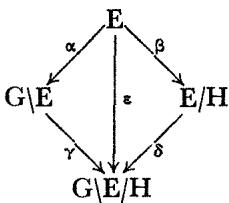
\includegraphics[keepaspectratio]{images/part001_b92675b5.jpg}}

（其中 \(\alpha, \beta, \gamma, \delta, \varepsilon\) 表示取商的典范映射）， \(\gamma \circ \alpha = \delta \circ \beta = \varepsilon\) 。

设 G 为一个群，H 为 G 的子群。考虑 H 通过右平移在 G 上的右作用（第 1 号，例 2）。轨道集合 G/H 是模 H 的左陪集集合；注意 G 依法则 \((g, xH) \mapsto gxH\) 在 G/H 上左作用（参见第 5 号）。类似地，模 H 的右陪集集合是 H 通过左平移在 G 上左作用的轨道集合 \(H\backslash G\) 。若 K 是 G 的包含 H 的子群，且 \(\Gamma\) 是模 H 的左（相应地，右）陪集，则 \(\Gamma K\) （相应地，\(K\Gamma\) ）是模 K 的左（相应地，右）陪集。映射 \(\Gamma \mapsto \Gamma K\) （相应地，\(\Gamma \mapsto K\Gamma\) ）称为 G/H 到 G/K（相应地，\(H\backslash G\) 到 \(K\backslash G\) ）的典范映射。它是满射。

设 G 为一个群，H 和 K 为 G 的两个子群。令 H 通过左平移在 G 上左作用，K 通过右平移在 G 上右作用；这两个作用可交换，故可考虑集合 \(H\backslash G/K\) 。\(H\backslash G/K\) 的元素称为 G 模 H 与 K 的双陪集。当 K = H 时，简称模 H 的双陪集。G/H 到 \(H\backslash G/H\) 上的典范映射是双射，当且仅当 H 是 G 的正规子群。

\subsection{齐次集合}

定义 6. 设 G 为一个群。G 在集合 E 上的作用称为传递的，如果存在元素 \(x \in E\) ，其轨道为 E。若 G 在 E 上的作用是传递的，则称 G-集 E 为齐次的。

也称 G 在 E 上传递地作用；或者说 E 是 G 下的齐次集。这等价于说 E 非空，且对 E 的任意元素 x 和 y，存在元素 \(\alpha \in G\) 使得 \(\alpha.x = y\) 。

例。若 E 是一个 G-集，则 E 的每个轨道（带诱导作用）都是 G 下的齐次集。

设 G 是一个群，H 是 G 的一个子群。考虑模 H 的左陪集集合 G/H。群 G 依法则 \((g, xH) \mapsto gxH\) 在 G/H 上左作用。设 N 为 H 的正规化子。群 N 依法则 \((xH, n) \mapsto xHn = xnH\) 在 G/H 上右作用。此作用在 H 上诱导出平凡作用，从而在取商后，N/H 在 G/H 上右作用。设 \(\phi: (N/H)^{0} \to S_{G/H}\) 为与此作用对应的同态。

命题 5. 在上述记号下，G/H 是一个齐次 G-集。映射 \(\phi\) 诱导出 \((\mathrm{N} / \mathrm{H})^0\) 到 G-集 G/H 的自同构群上的同构。

元素 \(\dot{e}=H\) 在 G/H 中的轨道是 G/H，由此得第一个断言。我们现在证明第二个断言。若 \(n\in N\) 通过右平移在 G/H 上定义的是恒等映射，则 \(\dot{e}.n=\dot{e}\) ，即 H.n=H，从而 \(n\in H\) 。因此

N/H 在 G/H 上右侧忠实作用，且 \(\phi\) 是单射。G 在 G/H 上的左作用与 N/H 在 G/H 上的右作用可交换，因此 N/H 的算子给出 G/H 到自身的 G-态射；由于它们是双射，这些态射必然是 G-自同构。于是 \(\phi\) 取值于 G/H 的 G-自同构所成的群 \(\Phi\) 。我们证明 \(\phi\) 的像就是 \(\Phi\) 。设 \(f \in \Phi\) 。通过结构转移，\(f(\dot{e})\) 在 G 中的稳定化子等于 \(\dot{e}\) 的稳定化子，即等于 H。设 \(n \in G\) 使得 \(f(\dot{e}) = n\dot{e}\) 。\(n\dot{e}\) 在 G 中的稳定化子是 \(nHn^{-1}\) （第 2 号，命题 2），因此 \(nHn^{-1} = H\) ，即 \(n \in N\) 。对 G/H 的每个元素 xH，有 \(f(xH) = f(x.\dot{e}) = x.f(\dot{e}) = xnH = xHn\) ，故 f 与由 n 定义的映射一致。

注记.(1) 设 G 是一个群，H 是 G 的一个子群，且 \(\phi: \mathbf{G} \to \mathfrak{S}_{\mathbf{G}/\mathbf{H}}\) 是对应于 G 在 G/H 上作用的同态。\(\phi\) 的核是 H 的诸共轭子群的交集（第 2 号，命题 2）。它也是包含在 H 中的最大正规子群（第 3 号）。特别地，G 忠实作用于 G/H 当且仅当 H 的诸共轭子群的交集缩减为 \(\{e\}\) 。

\begin{enumerate}
\def\labelenumi{(\arabic{enumi})}
\setcounter{enumi}{1}
\tightlist
\item
  设 G 为一个群，H 与 K 为其子群，且 H 是 K 的正规子群。则 K/H 在 G-集 G/H 上右作用，且 G/H 到 G/K 的典范映射在取商后定义出 G-集同构 \((G/H)/(K/H) \rightarrow G/K\) （参见第 4 号）。
\end{enumerate}

命题 6. 设 G 是一个群，E 是一个齐次 G-集， \(a \in E\) ，H 是 \(a\) 的稳定化子，且 K 是 G 中包含于 H 的子群。存在唯一的 G-态射 \(f\) ：G/K 到 E，使得 \(f(e.K) = a\) 。若 K = H，则 \(f\) 是同构。

若 \(f\) 是一个解，则 \(f(x, \mathbf{K}) = x.a\) 对所有 \(x\) 属于 \(\mathbf{G}\) 者成立，由此得唯一性；我们证明存在性。由 \(a\) 定义的轨道映射与等价关系 \(y \in x\mathbf{K}\) 在 \(\mathbf{G}\) 上相容。因为，若 \(y = xk, k \in \mathbf{K}\) ，则

\[
y. a = x k. a = x. a.
\]

映射 \(f\) 便这样由 \(G / K\) 导出到 \(H\) ，它满足 \(f(x, \mathbf{K}) = x.a\) 对所有 \(x\) 属于 \(G\) 成立。此映射是一个 G-态射，且 \(f(\mathbf{K}) = a\) 。此映射是满射的，因为它的像是 \(E\) 的一个非空稳定子集。现在设 \(K = H\) ，我们证明 \(f\) 是单射。若 \(f(x, \mathbf{H}) = f(y, \mathbf{H})\) ，则 \(x.a = y.a\) ，从而 \(x^{-1}y.a = a\) ，即 \(x^{-1}y \in H\) ，于是 \(x.H = y.H\) 。

定理 1. 设 G 是一个群。

\begin{enumerate}
\def\labelenumi{(\alph{enumi})}
\item
  每个齐次 G-集都同构于形如 G/H 的齐次 G-集，其中 H 是 G 的一个子群。
\item
  设 H 和 H' 是 G 的两个子群。G-集 G/H 与 G/H' 同构当且仅当 H 与 H' 共轭。
\end{enumerate}

由于齐次 G-集非空，断言 (a) 由命题 6 得出。我们证明 (b)。设 \(f: \mathrm{G} / \mathrm{H} \to \mathrm{G} / \mathrm{H}'\) 是一个 G-集同构。子群 H 是 H 的稳定化子，因此通过结构转移，它是 G/H' 中某元素的稳定化子。于是子群 H 与 H' 共轭（第 2 号，命题 2）。若 H' = αHα⁻¹，则 H' 是元素 α. H 在 G/H 中的稳定化子（第 2 号，命题 2），因此 G/H' 同构于 G/H（命题 6）。

例子。(1) 设 E 是一个非空集合。群 \(S_{E}\) 在 E 上传递地作用。若 x 和 y 是 E 的两个元素，则映射 \(\tau: E \to E\) （ \(\tau(x) = y\) , \(\tau(y) = x\) ，且 \(\tau(z) = z\) 对 \(z \neq x\) , y 成立）是 E 的一个置换。设 \(a \in E\) 。a 的稳定化子等同于 \(S_{F}\) ，其中 \(F = E - \{a\}\) 。于是齐次 G-集 E 同构于 \(S_{E}/S_{F}\) 。

\begin{enumerate}
\def\labelenumi{(\arabic{enumi})}
\setcounter{enumi}{1}
\tightlist
\item
  设 \(\mathbf{E}\) 是含 \(n\) 个元素的集合，\((p_i)_{i\in \mathbf{I}}\) 是整数 \(>0\) 的有限族，使得 \(\sum_{i}p_{i} = n\) 。设 \(\mathbf{X}\) 是形如 \((\mathrm{F}_i)_{i\in \mathbf{I}}\) 的 \(\mathbf{E}\) 的分拆中满足 \(\operatorname {Card}(\mathrm{F}_i) = p_i\) （对所有 \(i\) ）者所成的集合。群 \(\mathfrak{S}_{\mathbf{E}}\) 在 \(\mathbf{X}\) 上传递地作用。元素 \((\mathrm{F}_i)_{i\in \mathbf{I}}\) （属于 \(\mathbf{X}\) ）的稳定化子 H 典范同构于 \(\prod_{i\in \mathbf{I}}\mathfrak{S}_{\mathbf{F}_i}\) ，从而其阶为 \(\prod_{i\in \mathbf{I}}p_i!\) 。应用定理 1 与 §4，第 4 号，命题 4 的推论，可得到下述事实的一个新证明：
\end{enumerate}

\[
\operatorname{Card} (\mathbf {X}) = \frac {n !}{\prod_ {i \in I} p _ {i} !}.
\]

特别地，取 \(\mathbf{I} = \{1,2,\dots,r\}\) , \(\mathbf{E} = \{1,2,\dots,n\}\) ,

\[
\mathrm{F} _ {i} = \left\{p _ {1} + \dots + p _ {i - 1} + 1, \dots , p _ {1} + \dots + p _ {i} \right\}
\]

对 \(1 \leqslant i \leqslant r\) ，设 \(S\) 为 \(\tau \in \mathfrak{S}_{E}\) 中使 \(\tau|_{F_i}\) 对 \(1 \leqslant i \leqslant r\) 递增者所成的集合。若 \((G_1, \ldots, G_r) \in X\) ，则存在唯一的 \(\tau \in S\) 把 \((F_1, \ldots, F_r)\) 映为 \((G_1, \ldots, G_r)\) 。换言之，\(\mathfrak{S}_{E}\) 模 \(H\) 的每个左陪集与 \(S\) 恰好交于一点。

\begin{enumerate}
\def\labelenumi{(\arabic{enumi})}
\setcounter{enumi}{2}
\tightlist
\item
  *设 \(n\) 为整数 \(\geqslant 1\) 。正交群 \(\mathbf{O}(n, \mathbf{R})\) 在 \(\mathbf{S}_{n-1}\) （ \(\mathbf{R}^n\) 中的单位球面）上传递地作用。点 \((0, \ldots, 0, 1)\) 的稳定化子等同于正交群 \(\mathbf{O}(n-1, \mathbf{R})\) 。于是齐次 \(\mathbf{O}(n, \mathbf{R})\) -集 \(\mathbf{S}_{n-1}\) 同构于 \(\mathbf{O}(n, \mathbf{R}) / \mathbf{O}(n-1, \mathbf{R})\) 。*
\end{enumerate}

\subsection{齐次主集}

定义 7. 设 G 为一个群。G 在集合 E 上的一个作用称为单传递的，如果存在 E 中的一个元素 x，使得由 x 定义的轨道映射是双射。集合 E 连同 G 在 E 上的一个单传递左作用，称为 G 下的左齐次主 G-集（或 G 下的左齐次主集）。

这等同于说 G 在 E 上自由且传递地作用，或者也说存在一个元素 \(x \in E\) 使得由 x 定义的轨道映射是 G-集 G（其中 G 通过左平移作用）到 E 的一个同构；或者等价地，满足以下两个条件：

\begin{enumerate}
\def\labelenumi{(\roman{enumi})}
\item
  E 是非空的。
\item
  对于所有元素 \(x\) 和 \(y\) 于 \(\mathbf{E}\) ，存在且仅存在一个元素 \(\alpha \in \mathbf{G}\) 的集合，使得 \(\alpha x = y\) .
\end{enumerate}

条件(ii)也等价于以下条件：

\begin{enumerate}
\def\labelenumi{(\roman{enumi})}
\setcounter{enumi}{2}
\tightlist
\item
  映射 \((\alpha, x) \mapsto (\alpha x, x)\) 是从 \(G \times E\) 到 \(E \times E\) .
\end{enumerate}

我们将定义右齐次主 G-集的任务留给读者。

例子。(1) 设 G 通过左（相应地，右）平移作用于自身。这样便在 G 上定义了一个左（相应地，右）齐次主 G-集结构，它有时记为 \(G_{s}\) （相应地，\(G_{d}\) ）。

\begin{enumerate}
\def\labelenumi{(\arabic{enumi})}
\setcounter{enumi}{1}
\item
  设 E 是交换群 G 下的齐次集。若 G 忠实作用于 E，则后者是齐次主 G-集。
\item
  设 E 和 F 是两个同构的、带同一种类结构的集合，令 \(\operatorname{Isom}(\mathbf{E}, \mathbf{F})\) 为 E 到 F 上（带给定结构的）同构所成的集合。E 的（带给定结构的）自同构群 \(\operatorname{Aut}(\mathbf{E})\) 在 \(\operatorname{Isom}(\mathbf{E}, \mathbf{F})\) 上依法则 \((\sigma, f) \mapsto f \circ \sigma\) 右作用，且 \(\operatorname{Isom}(\mathbf{E}, \mathbf{F})\) 是一个右齐次主 \(\operatorname{Aut}(\mathbf{E})\) -集。类似地，群 \(\operatorname{Aut}(\mathbf{F})\) 在 \(\operatorname{Isom}(\mathbf{E}, \mathbf{F})\) 上依法则 \((\sigma, f) \mapsto \sigma \circ f\) 左作用，且 \(\operatorname{Isom}(\mathbf{E}, \mathbf{F})\) 是一个左齐次主 \(\operatorname{Aut}(\mathbf{F})\) -集。
\item
  *向量空间的加法群下的齐次主集称为仿射空间（参见 II，§ 9，第 1 号）。*
\end{enumerate}

齐次主 G-集 \(G_{s}\) （例 1）的自同构群是 G 的右平移群，它等同于 \(G^{0}\) （第 5 号，命题 5）。设 E 是一个齐次主 G-集，a 是 E 的一个元素。由 a 定义的轨道映射 \(\omega_{a}\) 是 G-集 \(G_{s}\) 到 E 上的同构。通过结构转移，得到一个同构 \(\psi_{a}\) ，它把 \(G^{0}\) 映到 Aut(E) 上。应当注意， \(\psi_{a}\) 一般依赖于 a；更确切地说，对于 \(\alpha \in G\) ，

\[
\psi_ {\alpha a} = \psi_ {a} \circ \operatorname{Int} _ {\mathbf {G} ^ {0}} (\alpha) = \psi_ {a} \circ \operatorname{Int} (\alpha^ {- 1}).\tag{3}
\]

因为，用 \(\delta_{a}\) 表示 G 上的平移 \(x\mapsto x\alpha\) ，

\[
\omega_ {\alpha a} = \omega_ {a} \circ \delta_ {\alpha}
\]

和

\[
\psi_ {a} (x) = \omega_ {a} \circ \delta_ {x} \circ \omega_ {a} ^ {- 1}, \quad x \in G,
\]

因此

\[
\psi_ {\alpha a} (x) = \omega_ {a} \circ \delta_ {\alpha} \circ \delta_ {x} \circ \delta_ {\alpha} ^ {- 1} \circ \omega_ {a} ^ {- 1} = \omega_ {a} \circ \delta_ {\alpha^ {- 1} x \alpha} \circ \omega_ {a} ^ {- 1} = \psi_ {a} (\alpha^ {- 1} x \alpha).
\]

\subsection{有限集合的置换群}

若 E 是含 n 个元素的有限集，则对称群 \(S_{E}\) （§ 4，第 1 号）是阶为 \(n!\) 的有限群。当 E 是自然数集 N 的区间 \([1, n]\) 时，相应的对称群记为 \(S_{n}\) ；任何含 n 个元素的集合的对称群都同构于 \(S_{n}\) 。

定义 8. 设 E 为有限集， \(\zeta \in \mathfrak{S}_{\mathrm{E}}\) 为 E 的一个置换， \(\bar{\zeta}\) 为 \(\mathfrak{S}_{\mathrm{E}}\) 中由 \(\zeta\) 生成的子群。\(\zeta\) 称为轮换，如果在 \(\bar{\zeta}\) 于 E 的作用下恰存在一条不缩减为单个元素的轨道。这条轨道称为 \(\zeta\) 的支集。

设 \(\zeta\) 为一个轮换。支集 \(\operatorname{supp}(\zeta)\) （即 \(\zeta\) 的支集）是由 \(x \in E\) 中满足 \(\zeta(x) \neq x\) 的元素组成的集合。

轮换 \(\zeta\) 的阶等于其支集的基数。子群 \(\bar{\zeta}\) 由 \(\zeta\) 生成，它在 \(\operatorname{supp}(\zeta)\) 上传递且忠实地作用。由于 \(\zeta\) 是交换的， \(\operatorname{supp}(\zeta)\) 是 \(\bar{\zeta}\) 下的一个主集（第 6 号，例 2），因此 \(\operatorname{Card}(\operatorname{supp}(\zeta)) = \operatorname{Card}(\bar{\zeta})\) 。

引理 1. 设 \((\zeta_{i})_{i\in I}\) 是一族支集两两不相交的轮换。则诸 \(\zeta_{i}\) 两两可交换。设 \(\sigma = \prod_{i\in I}\zeta_{i}\) ， \(\overline{\sigma}\) 为由 \(\sigma\) 生成的子群。则 \(\sigma(x) = \zeta_{i}(x)\) 对 \(x\in S_{i}, i\in I\) 成立，而 \(\sigma(x) = x\) 对 \(x\notin \bigcup_{i\in I}S_{i}\) 成立。映射 \(i\mapsto S_i\) 是 I 到不由单个元素组成的 \(\overline{\sigma}\) -轨道所成集合上的一个双射。

设 \(\zeta\) 和 \(\zeta'\) 是两个支集不相交的轮换。如果

\[
x \notin \operatorname{supp} (\zeta) \cup \operatorname{supp} \left(\zeta^ {\prime}\right),
\]

则 \(\zeta\zeta'(x) = \zeta'\zeta(x) = x\) 。若 \(x\) 属于 \(\zeta\) 的支集，则 \(\zeta'(x) = x\) 且 \(\zeta(x)\) 属于 \(\zeta\) 的支集，因此 \(\zeta\zeta'(x) = \zeta'\zeta(x) = \zeta(x)\) 。类似地，当 \(x\) 属于 \(\zeta'\) 的支集时， \(\zeta'\zeta(x) = \zeta\zeta'(x) = \zeta'(x)\) 。因此 \(\zeta\zeta' = \zeta'\zeta\) 。于是诸 \(\zeta_i\) 两两可交换，且对于 \(i \in I\) 和 \(x \in S_i\) , \(\sigma(x) = \zeta_i(x) \in S_i\) 。映射 \(\sigma\) 与 \(\zeta_i\) 在 \(S_i\) 上重合，故 \(S_i\) 在 \(\sigma\) 下稳定，且 \(\mathfrak{S}_{S_i}\) 中由 \(\sigma\) 在 \(S_i\) 上的限制所生成的子群在 \(S_i\) 上传递地作用；因此 \(S_i\) 是一条 \(\overline{\sigma}\) -轨道。由于诸 \(S_i\) 非空且两两不相交，映射 \(i \mapsto S_i\) 是单射。由于 \(\bigcup_{i} S_i\) 是 \(x\) 满足 \(\sigma(x) \neq x\) 的那些元素组成的集合，每条不由单个元素组成的 \(\overline{\sigma}\) -轨道都是某个 \(S_i\) 。

命题 7. 设 E 是一个有限集，且 \(\sigma\) 是 E 的一个置换。存在唯一的由轮换组成的有限集 C，满足以下两个条件：

\begin{enumerate}
\def\labelenumi{(\alph{enumi})}
\item
  C 中元素的支集两两不相交；
\item
  \(\sigma = \prod_{\zeta \in C} \zeta\) （由引理 1 ， \(C\) 的元素两两可交换）。设 \(\bar{\sigma}\) 为由 \(\sigma\) 生成的子群， \(S\) 为不由单个元素组成的 \(\bar{\sigma}\) -轨道所成的集合。对 \(s \in S\) ，令 \(\zeta_s(x) = \sigma(x)\) （若 \(x \in s\) ），并令 \(\zeta_s(x) = x\) （若 \(x \notin s\) ）。对所有 \(s \in S\) , \(\zeta_s\) 是支集为 \(s\) 的一个轮换，且 \(\sigma = \prod_{s \in S} \zeta_s\) ，这只需把两边作用于 \(E\) 的任意元素即可看出。\(C\) 的唯一性由引理 1 可得。
\end{enumerate}

定义 9. 2 阶轮换称为对换。

设 \(x\) 和 \(y\) 是 \(E\) 的两个不同元素。用 \(\tau_{x,y}\) 表示支集为 \(\{x, y\}\) 的唯一的对换。

对 E 的每个置换 \(\sigma\) ，置换 \(\sigma. \tau_{x,y}. \sigma^{-1}\) 是支集为 \(\{\sigma(x), \sigma(y)\}\) 的一个对换。因此：

\[
\sigma . \tau_ {x, y}. \sigma^ {- 1} = \tau_ {\sigma (x), \sigma (y)}.\tag{4}
\]

于是，对换在群 \(\mathfrak{S}_{\mathbb{E}}\) 中构成一个共轭类。

命题 8. 设 E 为有限集。群 \(\mathfrak{S}_{\mathrm{E}}\) 由对换生成。

对每个置换 \(\sigma\) ，令 \(F_{\sigma}\) 为由 \(x \in E\) 中满足 \(\sigma(x) = x\) 的元素组成的集合。我们对 \(p\) 作递降归纳来证明：每个置换 \(\sigma\) ，只要 \(\operatorname{Card}(F_{\sigma}) = p\) ，就是对换之积。若 \(p \geqslant \operatorname{Card}(E)\) ，则置换 \(\sigma\) 是 \(E\) 的恒等映射；它是对换的空族之积。若 \(p < \operatorname{Card}(E)\) ，设性质已对每个置换 \(\sigma'\) （ \(\operatorname{Card}(F_{\sigma'}) > p\) ）证明。现在 \(E - F_{\sigma} \neq \varnothing\) ；取 \(x \in E - F_{\sigma}\) 及 \(y \in \sigma(x)\) 。则 \(y \neq x\) 且 \(y \in E - F_{\sigma}\) 。令 \(\sigma' = \tau_{x,y} \cdot \sigma\) 。集合 \(F_{\sigma'}\) 包含 \(F_{\sigma}\) 与 \(x\) ，故 \(\operatorname{Card}(F_{\sigma'}) > \operatorname{Card}(F_{\sigma}) = p\) 。由归纳假设， \(\sigma'\) 是对换之积，从而 \(\sigma = \tau_{x,y} \cdot \sigma'\) 是对换之积。

命题 9. 设 \(n\) 为整数 \(\geqslant 0\) 。群 \(\mathfrak{S}_n\) 由诸对换 \((\tau_{i,i+1})_{1\leqslant i\leqslant n-1}\) 生成。

根据命题 8 ，只需证明每个对换 \(\tau_{p,q}\) （ \(1 \leqslant p < q \leqslant n\) ）属于由诸 \(\tau_{i,i+1}\) （ \(1 \leqslant i \leqslant n-1\) ）生成的子群 H 。我们对 \(q-p\) 作归纳来证明这一点。对 \(q-p=1\) ，这是显然的。若 \(q-p>1\) ，则（公式 (4)） \(\tau_{p,q} = \tau_{q-1,q}\tau_{p,q-1}\tau_{q-1,q}\) 。由归纳假设 \(\tau_{p,q-1} \in H\) ，从而 \(\tau_{p,q} \in H\) 。

若 \(\sigma \in \mathfrak{S}_n\) ，则每个有序对 \((i,j)\) （ \([1,n]\) 的元素，满足 \(i < j\) 且 \(\sigma(i) > \sigma(j)\) ）称为 \(\sigma\) 的一个逆序。用 \(\nu(\sigma)\) 表示 \(\sigma\) 的逆序的个数。

设 P 为从 \(Z^{n}\) 到 Z 的映射所成的加法群。对 \(f \in P\) 与 \(\sigma \in S_{n}\) ，令 \(\sigma f\) 为 P 中由下式定义的元素

\[
\sigma f (z _ {1}, \dots , z _ {n}) = f (z _ {\sigma (1)}, \dots , z _ {\sigma (n)}).\tag{5}
\]

这样定义的 \(\mathfrak{S}_n\) 在 \(\mathbf{P}\) 上的作用是一个群作用；对所有 \(\sigma, \tau \in \mathfrak{S}_n\) 和 \(f \in \mathbf{P}, ef = f\) 且

\[
\begin{array}{r l} \left(\tau (\sigma f)\right) (z _ {1}, \dots , z _ {n}) & = \sigma f (z _ {\tau (1)}, \dots , z _ {\tau (n)}) = f (z _ {\tau \sigma (1)}, \dots , z _ {\tau \sigma (n)}) \\ & = ((\tau \sigma) f) (z _ {1}, \dots , z _ {n}). \end{array}
\]

公式 (5) 表明 \(\sigma(-f) = -\sigma f\) 对 \(\sigma \in \mathfrak{S}_n\) 和 \(f \in P\) 成立。

设 \(p\) 为 P 中由下式定义的元素

\[
p (z _ {1}, \dots , z _ {n}) = \prod_ {i <   j} (z _ {j} - z _ {i}).\tag{6}
\]

引理 2. \(p \neq 0\) ，且 \(\sigma p = (-1)^{\nu(\sigma)}\) 对 \(\sigma \in \mathfrak{S}_n\) 成立。

\(p(1,2,\ldots,n) = \prod_{i < j}(j - i)\neq 0\) ，因此 \(p\neq 0\) 。另一方面，若 \(\sigma \in \mathfrak{S}_n\) ，则

\[
\sigma p (z _ {1}, \dots , z _ {n}) = p (z _ {\sigma (1)}, \dots , z _ {\sigma (n)}) = \prod_ {i <   j} (z _ {\sigma (j)} - z _ {\sigma (i)}).
\]

设 C 为有序对 \((i,j)\) 所成的集合，满足 \(1 \leqslant i \leqslant n\) , \(1 \leqslant j \leqslant n\) ， i \textless{} j 。在 C 上定义置换 \(\theta\) 如下：令 \(\theta(i,j) = (\sigma(i), \sigma(j))\) 若 \((i,j)\) 不是逆序；令 \(\theta(i,j) = (\sigma(j), \sigma(i))\) 若 \((i,j)\) 是逆序。由此可得 \(\sigma p = (-1)^{\nu(\sigma)} p\) 。

定理 2. 设 E 是一个有限集。存在唯一的同态 \(\varepsilon\) ：从 \(\mathfrak{S}_n\) 到乘法群 \(\{-1, +1\}\) ，使 \(\varepsilon(\tau) = -1\) 对每个对换 \(\tau\) 成立。

唯一性由命题 8 得出。我们证明存在性。通过结构转移，可设 \(\mathbf{E} = [1, n]\) 。采用上述记号，令 \(\varepsilon(\sigma) = (-1)^{\nu(\sigma)}\) 。则（引理 2）

\[
\sigma (\sigma^ {\prime} p) = \sigma (\varepsilon (\sigma^ {\prime}) p) = \varepsilon (\sigma^ {\prime}) (\sigma p) = \varepsilon (\sigma^ {\prime}) \varepsilon (\sigma) p.
\]

另一方面，

\[
\sigma (\sigma^ {\prime} p) = (\sigma \sigma^ {\prime}) p = \varepsilon (\sigma \sigma^ {\prime}) p.
\]

由于 \(p \neq -p\) ，由此可得 \(\varepsilon(\sigma\sigma') = \varepsilon(\sigma)\varepsilon(\sigma')\) ，故 \(\varepsilon\) 是一个同态。我们现在证明，对每个对换 \(\tau, \varepsilon(\tau) = -1\) 。\(\nu(\tau_{n-1,n}) = 1\) ，故 \(\varepsilon(\tau_{n-1,n}) = -1\) 。由于每个对换 \(\tau\) 都与 \(\tau_{n-1,n}\) 共轭，且群 \(\{-1, +1\}\) 是交换的，故 \(\varepsilon(\tau) = \varepsilon(\tau_{n-1,n}) = -1\) 。

定义 10. 在定理 2 的记号下，数 \(\varepsilon(\sigma)\) （也记作 \(\varepsilon_{\sigma}\) ）称为置换 \(\sigma\) 的符号。同态 \(\varepsilon\) 的核称为 E 的交错群。

\(\sigma\) 称为偶置换（相应地，奇置换），如果 \(\varepsilon(\sigma) = 1\) （相应地， \(\varepsilon(\sigma) = -1\) ）。E 的交错群记为 \(\mathfrak{A}_{\mathbb{E}}\) 。它是 \(\mathfrak{S}_{\mathbb{E}}\) 的一个正规子群。当 \(\mathbf{E} = [1, n]\) 时，简记为 \(\mathfrak{A}_{n}\) 。当 E 的基数 \(n\) 为 \(\geqslant 2\) 时，它是指数为 2 的子群，因此阶为 \(n! / 2\) 。可以证明，对 \(n = 3\) 或 \(n \geqslant 5\) ，群 \(\mathfrak{A}_{n}\) 是单群（参见习题 16）。

例。若 \(\sigma\) 是一个阶为 \(d\) 的轮换，则

\[
\varepsilon (\sigma) = (- 1) ^ {d - 1}.
\]

置换的逆序数

\[
(1, 2, 3, \dots , d) \mapsto (d, 1, 2, \dots , d - 1)
\]

等于 \(d - 1\) 。

\section{扩张、可解群、幂零群}

在本段中，除非另有明确说明，群运算均以乘法形式书写。

\subsection{扩张}

定义 1. 设 F 和 G 是两个群。G 被 F 的扩张是一个三元组 \(\mathcal{E} = (\mathrm{E}, i, p)\) ，其中 E 是一个群， \(i\) 是 F 到 E 内的单射同态， \(p\) 是 E 到 G 上的满射同态，使得 \(\operatorname{Im}(i) = \operatorname{Ker}(p)\) 。同态 \(s: \mathrm{G} \to \mathrm{E}\) （相应地， \(r: \mathrm{E} \to \mathrm{F}\) ），若满足 \(p \circ s = \operatorname{Id}_{\mathbf{G}}\) （相应地， \(r \circ i = \operatorname{Id}_{\mathbf{F}}\) ），则称为扩张 \(\mathcal{E}\) 的截面（相应地，收缩）。

扩张 \(\mathcal{E} = (\mathrm{E}, i, p)\) （ \(\mathbf{G}\) 被 \(\mathbf{F}\) 的扩张）常用图表 \(\mathcal{E}: \mathrm{F} \xrightarrow{i} \mathrm{E} \xrightarrow{p} \mathrm{G}\) 表示，其中 \(i\) 和 \(p\) 在不会引起混淆时有时省略。有时也简单地说群 \(\mathbf{E}\) 是 \(\mathbf{G}\) 被 \(\mathbf{F}\) 的扩张。

群 E 是 G 被 F 的扩张，当且仅当它包含一个同构于 F 的正规子群 \(F'\) ，使得商群 \(E/F'\) 同构于 G。

一个扩张 \(\mathcal{E}\colon\mathrm{F}\xrightarrow{i}\mathrm{E}\xrightarrow{p}\mathrm{G}\) 称为中心扩张，如果像 \(i(\mathrm{F})\) 包含在 E 的中心内；这仅当 F 是交换群时才可能。

设 \(\mathcal{E}:\mathrm{F}\xrightarrow{i}\mathrm{E}\xrightarrow{p}\mathrm{G}\) 和 \(\mathcal{E}':\mathrm{F}\xrightarrow{i'}\mathrm{E}'\xrightarrow{p'}\mathrm{G}\) 是 G 被 F 的两个扩张。\(\mathcal{E}\) 到 \(\mathcal{E}'\) 的态射是一个同态 \(u:\mathrm{E}\to\mathrm{E}'\) ，满足 \(p'\circ u=p\) 与 \(u\circ i=i'\) ，或者换句话说，使得下图交换：

\pandocbounded{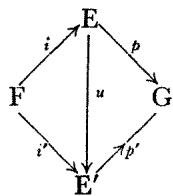
\includegraphics[keepaspectratio]{images/part001_e41623d9.jpg}}

命题 1. 设 \(\mathcal{E}: F \xrightarrow{i} E \xrightarrow{p} G\) 和 \(\mathcal{E}': F \xrightarrow{i'} E' \xrightarrow{p'} G\) 是 \(G\) 被 \(F\) 的扩张。若 \(u: E \to E'\) 是 \(\mathcal{E}\) 到 \(\mathcal{E}'\) 的态射，则 \(u\) 是 \(E\) 到 \(E'\) 上的同构，且 \(u^{-1}\) 是 \(\mathcal{E}'\) 到 \(\mathcal{E}\) 的态射。

设 \(x \in E\) 满足 \(u(x) = e\) 。则 \(p(x) = p'(u(x)) = e\) ，因此 \(x \in i(F)\) 。设 \(y \in F\) 满足 \(x = i(y)\) ；则 \(i'(y) = u(i(y)) = e\) 。由于 \(i'\) 是单射，有 \(y = e\) 与 \(x = e\) 。因此 \(u\) 是单射。根据 §4 第 6 号命题 7 的推论 1 ， \(u\) 是满射，因为 \(u(i(F)) = i'(F)\) 。最后一个断言是显然的。

换句话说，扩张 \(\mathcal{E}\) 与 \(\mathcal{E}'\) 同构，当且仅当存在 \(\mathcal{E}\) 到 \(\mathcal{E}'\) 的态射。

设 \(\mathbf{F}\) 和 \(\mathbf{G}\) 是两个群，记 \(\mathbf{E}_0 = \mathbf{F} \times \mathbf{G}\) ；令 \(i: \mathbf{F} \to \mathbf{E}_0\) 为典范单射， \(p: \mathbf{E}_0 \to \mathbf{G}\) 为典范投影。\(\mathbf{G}\) 被 \(\mathbf{F}\) 的扩张中，凡同构于扩张 \(\mathcal{E}_0: \mathbf{F} \xrightarrow{i} \mathbf{E}_0 \xrightarrow{p} \mathbf{G}\) 者，都称为平凡扩张。

命题 2. 设 \(\mathcal{E}:\mathrm{F}\xrightarrow{i}\mathrm{E}\xrightarrow{p}\mathrm{G}\) 是 \(\mathrm{G}\) 被 \(\mathrm{F}\) 的一个扩张。下列条件等价：

\begin{enumerate}
\def\labelenumi{(\roman{enumi})}
\item
  \(\mathcal{E}\) 是一个平凡扩张；
\item
  \(\mathcal{E}\) 有一个收缩 \(r\) ；
\item
  \(\mathcal{E}\) 有一个截面 \(s\) ，使得 \(s(\mathbf{G})\) 包含于 \(i(\mathbf{F})\) 的中心化子中；
\end{enumerate}

显然 (i) 蕴含 (ii) 与 (iii)。若 (ii) 成立，则映射 \((r, p): \mathbf{E} \to \mathbf{F} \times \mathbf{G}\) 是 \(\mathcal{E}\) 到 \(\mathcal{E}_0\) 的态射，由此得 (i)。若 (iii) 成立，则从 \(\mathbf{F} \times \mathbf{G}\) 到 \(\mathbf{E}\) 的、对应于 \((i, s)\) 的同态（ \(\S 4\) ，第 9 号，命题 12）是 \(\mathcal{E}_0\) 到 \(\mathcal{E}\) 的态射，由此得 (i)。

可能有这样的情形：扩张 \(\mathcal{E}:\mathbf{F}\to\mathbf{E}\to\mathbf{G}\) 并不平凡，而群 \(\mathbf{E}\) 却同构于 \(\mathbf{F}\times\mathbf{G}\) （习题 6）。

定义 2. 设 F 和 G 是两个群， \(\tau\) 是 G 到 F 的自同构群的一个同态。记 \(\tau(g)(f) = {}^g f\) （对 \(g \in G\) 与 \(f \in F\) ）。集合 \(\mathbf{F} \times \mathbf{G}\) 赋以合成律

\[
((f, g), (f ^ {\prime}, g ^ {\prime})) \mapsto (f, g) \cdot_ {\tau} (f ^ {\prime}, g ^ {\prime}) = (f. ^ {g} f ^ {\prime}, g g ^ {\prime})\tag{1}
\]

称为 G 与 F 关于 \(\tau\) 的外半直积。

G 与 F 关于 \(\tau\) 的外半直积记作 \(F \times_{\tau} G\) 。

命题 3. 外半直积 \(\mathbf{F} \times_{\tau} \mathbf{G}\) 是一个群。映射 \(i: \mathbf{F} \to \mathbf{F} \times_{\tau} \mathbf{G}\) 由 \(i(f) = (f, e)\) 定义，映射 \(p: \mathbf{F} \times_{\tau} \mathbf{G} \to \mathbf{G}\) 由 \(p(f, g) = g\) 定义，映射 \(s: \mathbf{G} \to \mathbf{F} \times_{\tau} \mathbf{G}\) 由 \(s(g) = (e, g)\) 定义，它们都是群同态。三元组 \((\mathbf{F} \times_{\tau} \mathbf{G}, i, p)\) 是 \(\mathbf{G}\) 被 \(\mathbf{F}\) 的一个扩张，而 \(s\) 是该扩张的一个截面。

我们有：

\[
\begin{array}{r l} ((f, g) \cdot_ {\tau} (f ^ {\prime}, g ^ {\prime})) \cdot_ {\tau} (f ^ {\prime \prime}, g ^ {\prime \prime}) & = (f. ^ {g} f ^ {\prime}, g g ^ {\prime}) \cdot_ {\tau} (f ^ {\prime \prime}, g ^ {\prime \prime}) \\ & = (f. ^ {g} f ^ {\prime}. ^ {g g ^ {\prime}} f ^ {\prime \prime}, g g ^ {\prime} g ^ {\prime \prime}); \\ (f, g) \cdot_ {\tau} ((f ^ {\prime}, g ^ {\prime}) \cdot_ {\tau} (f ^ {\prime \prime}, g ^ {\prime \prime})) & = (f, g) \cdot_ {\tau} (f ^ {\prime}. ^ {g ^ {\prime}} f ^ {\prime \prime}, g ^ {\prime} g ^ {\prime \prime}) \\ & = (f. ^ {g} (f ^ {\prime}. ^ {g ^ {\prime}} f ^ {\prime \prime}), g g ^ {\prime} g ^ {\prime \prime}). \end{array}
\]

现在， \({}^{g}(f'.{}^{g'}f'') = {}^{g}f'.{}^{gg'}f''\) ，这表明由 (1) 定义的合成律是结合的。元素 \((e, e)\) 是该律下的单位元。元素 \((f, g)\) 以 \((^{g^{-1}}f^{-1}, g^{-1})\) 为逆元。因此 \(F \times_{\tau} G\) 上的合成律是群律。其余断言是显然的。

采用命题 3 的记号，用 \(E_{\tau}\) 表示扩张

\[
\mathrm{F} \xrightarrow {i} \mathrm{F} \times_ {\tau} \mathrm{G} \xrightarrow {p} \mathrm{G}.
\]

设 \(\mathcal{E}'\colon F\stackrel{i'}{\to}E'\stackrel{p'}{\to}G\) 是 \(G\) 被 \(F\) 的扩张， \(s'\colon G\to E'\) 是 \(\mathcal{E}'\) 的一个截面。我们定义一个运算 \(\tau\) （ \(G\) 在群 \(F\) 上的运算）如下：

\[
i ^ {\prime} (\tau (g, f)) = s ^ {\prime} (g) i ^ {\prime} (f) s ^ {\prime} (g) ^ {- 1} = \operatorname{Int} (s ^ {\prime} (g)) (i ^ {\prime} (f)).\tag{2}
\]

命题 4. 采用上述记号，存在唯一的同构 \(u\) ，它把 \(\mathcal{E}_{\tau}\) 映到 \(\mathcal{E}'\) 上，使得 \(u \circ s = s'\) 。

\((f, g) = (f, e) \cdot_ {\tau} (e, g) = i(f).s(g)\) 。因此，如果 u 是该问题的一个解，则必然有 \(u(f,g)=i'(f).s'(g)\) ，从而 u 的唯一性成立。我们证明存在性。我们记 \(u(f,g)=i'(f).s'(g)\) 。则

\[
\begin{array}{r l} u (f, g) \cdot u (f ^ {\prime}, g ^ {\prime}) & = i ^ {\prime} (f) s ^ {\prime} (g) i ^ {\prime} (f ^ {\prime}) s ^ {\prime} (g ^ {\prime}) \\ & = i ^ {\prime} (f) (s ^ {\prime} (g) i ^ {\prime} (f ^ {\prime}) s ^ {\prime} (g) ^ {- 1}) s ^ {\prime} (g) s ^ {\prime} (g ^ {\prime}) \\ & = i ^ {\prime} (f) i ^ {\prime} (\tau (g, f ^ {\prime})) \cdot s ^ {\prime} (g) s ^ {\prime} (g ^ {\prime}) \\ & = i ^ {\prime} (f \cdot \tau (g, f ^ {\prime})) \cdot s ^ {\prime} (g g ^ {\prime}) \\ & = u ((f, g) \cdot_ {\tau} (f ^ {\prime}, g ^ {\prime})). \end{array}
\]

因此， \(u\) 是 \(\mathbf{F} \times_{\tau} \mathbf{G}\) 到 \(\mathbf{E}'\) 内的同态。显然 \(u \circ i = i'\) , \(p' \circ u = p\) 且 \(u \circ s = s'\) 。

注记。由公式 (2) 定义的运算 \(\tau\) 依赖于扩张 \(\mathcal{E}'\) 和截面 \(s'\) 。当 F 交换时，运算 \(\tau\) 不依赖于 \(s'\) 。因为此时 \(\operatorname{Int}(s'(g)) \mid i'(F)\) 仅依赖于 \(s'(g)\) 模 \(i'(F)\) 的陪集。

更一般地，设 \(\mathcal{E}:\mathrm{F}\to \mathrm{E}\to \mathrm{G}\) 是 \(\mathbf{G}\) 被交换群 \(\mathbf{F}\) 的一个扩张（并不假定 \(\mathcal{E}\) 有截面）。群 \(\mathbf{E}\) 经内自同构作用在 \(\mathbf{F}\) 上，该作用在 \(\mathbf{F}\) 的像上平凡，从而定义了 \(\mathbf{G}\) 在 \(\mathbf{F}\) 上的一个作用。若 \(\mathcal{E}\) 有截面，则此作用就是由公式 (2) 定义的作用。

推论. 设 G 是一个群，H 和 K 是 G 的两个子群，使得 H 正规， \(\mathbf{H} \cap \mathbf{K} = \{e\}\) 且 \(\mathbf{H} \cdot \mathbf{K} = \mathbf{G}\) 。设 \(\tau\) 为 \(\mathbf{K}\) 在 \(\mathbf{H}\) 上的、经 \(\mathbf{G}\) 的内自同构定义的作用。映射 \((h, k) \mapsto hk\) 是 \(\mathbf{H} \times_{\tau} \mathbf{K}\) 到 \(\mathbf{G}\) 上的同构。

在此推论的假设下，称 G 为 K 被 H 的半直积。

例子。(1) 设 G 为一个群，E 为一个齐次主 G-集；用 \(\Gamma\) 表示 G 的自同构群。设 A 为 E 的具有下述性质的置换 f 所成的集合：

存在 \(\gamma \in \Gamma\) ，使得 \(f\) 是一个 \(\gamma\) -态射，从 \(\mathbf{E}\) 到 \(\mathbf{E}\) （即 \(f(gb) = \gamma(g)f(b)\) ，对 \(b \in \mathbf{E}\) 与 \(g \in \mathbf{G}\) ）。

上述公式 \(f(gb) = \gamma(g)f(b)\) 表明，若 \(f \in A\) ，则存在唯一的 \(\gamma \in \Gamma\) 使 \(f\) 为 \(\gamma\) -态射，我们把它记作 \(p(f)\) 。

设 \(f, f'\) 是 A 中的元素， \(\gamma = p(f), \gamma' = p(f')\) 。那么，对所有 \(b \in E\) 与所有 \(g \in G\) ，

\[
(f ^ {\prime} \circ f) (g b) = f ^ {\prime} (\gamma (g) f (b)) = \gamma^ {\prime} (\gamma (g)) f ^ {\prime} (f (b))
\]

这证明了 \(f' \circ f \in \mathbf{A}\) 且 \(p(f' \circ f) = p(f')p(f)\) 。另一方面， \(f(\gamma^{-1}(g)f^{-1}(b)) = gb\) ，因此 \(f^{-1}(gb) = \gamma^{-1}(g)f^{-1}(b)\) ，从而 \(f^{-1} \in \mathbf{A}\) 。于是 \(\mathbf{A}\) 是 \(\mathfrak{S}_{\mathbf{E}}\) 的子群， \(p\) 是 \(\mathbf{A}\) 到 \(\Gamma\) 的同态。\(p\) 的核是集合 \(\operatorname{Aut}_{\mathbf{G}}(\mathbf{E})\) ，即 \(\mathbf{G}\) -集 \(\mathbf{E}\) 的自同构组成的集合。

我们取定 \(a \in \mathbf{E}\) 。我们在 §5 第 6 号中定义过一个同构 \(\psi_a\) ，它把 \(\mathbf{G}^0\) 映到 \(\operatorname{Aut}_{\mathbf{G}}(\mathbf{E})\) 上，使得 \(\psi_a(x)(ga) = gxa\) ，其中 \(g, x\) 取遍 \(\mathbf{G}\) 。另一方面，对 \(\gamma \in \Gamma\) ，令 \(s_a(\gamma)\) 为 \(\mathbf{E}\) 的由 \(s_a(\gamma)(ga) = \gamma(g)a\) （对所有 \(g \in \mathbf{G}\) ）定义的置换；立即可验证 \(s_a\) 是 \(\Gamma\) 到 \(\mathbf{A}\) 的同态，且满足 \(p \circ s_a = \operatorname{Id}_{\Gamma}\) 。于是 \(\mathbf{G}^0 \xrightarrow{\psi_a} \mathbf{A} \xrightarrow{p} \Gamma\) 是 \(\Gamma\) 被 \(\mathbf{G}^0\) 的一个扩张，而 \(s_a\) 是该扩张的一个截面。这个扩张与这个截面定义了 \(\Gamma\) 在 \(\mathbf{G}^0\) 上的一个作用： \(s_a(\Gamma)\) 经内自同构作用在 \(\psi_a(\mathbf{G}^0)\) 上；我们把这个作用写成指数记法。我们证明这个作用是自然作用（§3，第 1 号，例 3）：对 \(x, g\) 属于 \(\mathbf{G}\) 以及 \(\gamma \in \Gamma\) ，

\[
\begin{array}{r l} (\psi_ {a} (^ {\gamma} x)) (g a) & = (s _ {a} (\gamma) \circ \psi_ {a} (x) \circ s _ {a} (\gamma) ^ {- 1}) (g a) \\ & = (s _ {a} (\gamma) \circ \psi_ {a} (x)) (\gamma^ {- 1} (g) a) = s _ {a} (\gamma) (\gamma^ {- 1} (g) x a) \\ & = g \gamma (x) a = \psi_ {a} (\gamma (x)) g a \end{array}
\]

，因此 \({}^{\gamma}x = \gamma(x)\) 。

于是命题 4 表明，A 同构于 \(\Gamma = \operatorname{Aut}(\mathbf{G})\) 被 \(\mathbf{G}^0\) 的半直积（在 \(\operatorname{Aut}(\mathbf{G})\) 对 \(\mathbf{G}^0\) 的自然作用下）。注意，我们所构造的同构一般依赖于元素 \(a \in \mathbf{E}\) 的选取。

\begin{enumerate}
\def\labelenumi{(\arabic{enumi})}
\setcounter{enumi}{1}
\tightlist
\item
  *设 A 为交换环。上三角群 T(n, A) 是对角子群 D(n, A) 被上严格三角群 T1(n, A) 的半直积。*
\end{enumerate}

\subsection{换位子}

定义 3. 设 G 为一个群，x 与 y 为 G 的两个元素。G 的元素 \(x^{-1}y^{-1}xy\) 称为 x 与 y 的换位子。

用 \((x,y)\) 表示 x 与 y 的换位子。于是显然

\[
(y, x) = (x, y) ^ {- 1}.
\]

对于 \(x\) 与 \(y\) ，可交换的充要条件是 \((x, y) = e\) 。更一般地，

\[
x y = y x (x, y).
\]

另一方面，我们记

\[
x ^ {y} = y ^ {- 1} x y = x (x, y) = (y, x ^ {- 1}) x.\tag{3}
\]

由于映射 \(x \mapsto x^y\) 是内自同构 \(\operatorname{Int}(y^{-1})\) ，故 \((x, y)^z = (x^z, y^z)\) 对所有 \(x, y, z \in G\) 成立。

对于 \(x, y, z \in G\) ，我们证明以下关系式：

\[
(x, y z) = (x, z). (x, y) ^ {z} = (x, z). (z, (y, x)). (x, y)\tag{4}
\]

(4 bis) \((xy,z) = (x,z)^y.(y,z) = (x,z).(((x,z),y).(y,z))\)

\begin{enumerate}
\def\labelenumi{(\arabic{enumi})}
\setcounter{enumi}{4}
\item
  \((x^{y}, (y, z)).(y^{z}, (z, x)).(z^{x}, (x, y)) = e\)
\item
  \((x, yz).(z, xy).(y, zx) = e\)
\end{enumerate}

(6 bis) \((xy, z). (yz, x). (zx, y) = e.\)

现在

\[
\begin{array}{r l} (x, y z) & = x ^ {- 1} z ^ {- 1} y ^ {- 1} x y z = (x, z) z ^ {- 1} x ^ {- 1} y ^ {- 1} x y z = (x, z) (x, y) ^ {z} \\ & = (x, z) (z, (x, y) ^ {- 1}) (x, y) \end{array}
\]

由 (3) 即得，这证明了 (4)。公式 (4 bis) 可类似地得到。另一方面，

\[
\begin{array}{r l} (x ^ {y}, (y, z)) & = (x ^ {y}) ^ {- 1} (z, y) (x ^ {y}) (y, z) \\ & = y ^ {- 1} x ^ {- 1} y z ^ {- 1} y ^ {- 1} z y y ^ {- 1} x y y ^ {- 1} z ^ {- 1} y z \\ & = (y z y ^ {- 1} x y) ^ {- 1} (z x z ^ {- 1} y z). \end{array}
\]

然后记 \(u = yzy^{-1}xy\) , \(v = zxz^{-1}yz\) 和 \(w = xyx^{-1}zx\) ，我们得到

\[
(x ^ {y}, (y, z)) = u ^ {- 1} v.
\]

通过循环置换 \(x, y, z\) ，我们推出 \((y^z, (z, x)) = v^{-1}w\) 和

\[
\left(z ^ {x}, (x, y)\right) = w ^ {- 1} u,
\]

这立即推出(5)。最后，(6)通过将x, y, z在公式 \((x, yz) = x^{-1}z^{-1}y^{-1}xyz = (yzx)^{-1}(xyz)\) 中循环置换所得三个公式的两边分别相乘而得到，对于(6 bis)也类似。

若 A 和 B 是 G 的两个子群，则 (A, B) 表示由诸换位子 \((a, b)\) （ \(a \in A\) ， \(b \in B\) ）生成的子群。于是 \((A, B) = \{e\}\) 当且仅当 A 中心化 B； \((A, B) \subset A\) 当且仅当 B 正规化 A。若 A 和 B 都是正规的（相应地，特征的），则 \((A, B)\) 亦然。

命题 5. 设 A、B、C 是 G 的三个子群。

\begin{enumerate}
\def\labelenumi{(\roman{enumi})}
\item
  子群A正规化子群(A, B)。
\item
  若子群 (B, C) 正规化 A，则子群 (A, (B, C)) 由诸元素 \((a, (b, c))\) （ \(a \in \mathbf{A}\) , \(b \in \mathbf{B}\) , \(c \in \mathbf{C}\) ）生成。
\item
  若 A、B 和 C 均为正规子群，则
\end{enumerate}

\[
(\mathrm{A}, (\mathrm{B}, \mathrm{C})) \subset (\mathrm{C}, (\mathrm{B}, \mathrm{A})). (\mathrm{B}, (\mathrm{C}, \mathrm{A})).
\]

由 (4 bis)，对 \(a, a' \in \mathbf{A}\) 与 \(b \in \mathbf{B}\) ，

\[
(a, b) ^ {a ^ {\prime}} = (a a ^ {\prime}, b). (a ^ {\prime}, b) ^ {- 1},
\]

由此得 (i)。现在假设 (B, C) 正规化 A。对于 \(a \in \mathbf{A}\) , \(b \in \mathbf{B}\) , \(c \in \mathbf{C}\) 和 \(x \in \mathbf{G}\) ，(4) 蕴含

\[
(a, (b, c). x) = (a, x). (x, ((b, c), a)) (a, (b, c))
\]

和 \(((b, c), a) \in \mathbf{A}\) ，因为 (B, C) 正规化 A；故由对 \(p\) 的归纳可知， \(\left(a, \prod_{i=1}^{p} (b_i, c_i)\right)\) （对 \(b_i \in \mathbf{B}\) , \(c_i \in \mathbf{C}\) ）属于由形如 \((a, (b, c))\) 的元素生成的子群。若最后 A、B、C 都是正规的，则子群 (A, (B, C))、(C, (B, A)) 与 (B, (C, A)) 也都是正规的。于是由 (ii)，只需证明

\[
(a, (b, c)) \in (\mathrm{C}, (\mathrm{B}, \mathrm{A})). (\mathrm{B}, (\mathrm{C}, \mathrm{A}))
\]

对所有 \(a \in \mathbf{A}\) , \(b \in \mathbf{B}\) 与 \(c \in \mathbf{C}\) 成立。现在由 (5)，记 \(a^{b^{-1}} = u\)

\[
(a, (b, c)) = ((u ^ {b}), (b, c)) = (c ^ {u}, (u, b)) ^ {- 1}. (b ^ {c}, (c, u)) ^ {- 1},
\]

由此得(iii)。

定义 4. 设 G 是一个群。由 G 中元素的换位子生成的子群称为 G 的导群。

G 的导群即子群 (G, G)。它也记作 D(G)。作为一种语言上的滥用，它有时被称为 G 的换位子群，尽管它一般不同于 G 中元素的换位子集合（习题 16）。D(G) = \{e\} 当且仅当 G 是交换的。

命题 6. 设 \(f: \mathbf{G} \to \mathbf{G}'\) 是群同态。则 \(f(\mathbf{D}(\mathbf{G})) \subset \mathbf{D}(\mathbf{G}')\) 。若 \(f\) 是满射，则 \(\mathbf{D}(\mathbf{G})\) 到 \(\mathbf{D}(\mathbf{G}')\) 的、由 \(f\) 的限制所得到的同态是满射。

\(f\) 把 \(G\) 中元素的换位子映为 \(G'\) 中元素的换位子。若 \(f\) 是满射，则 \(f\) 把 \(G\) 的换位子集合映为 \(G'\) 的换位子集合。于是该命题由 §4 第 3 号命题 2 的推论 3 得出。

推论1. 群G的导群是G的一个特征子群。特别地，它是G的一个正规子群。

推论 2. 设 G 是一个群。商群 G/D(G) 是交换的。设 \(\pi: G \to G/D(G)\) 为典范同态。每个同态 \(f\) （从 G 到交换群 \(G'\) ）都可唯一地表示为 \(f = \bar{f} \circ \pi\) 的形式，其中 \(\bar{f}: G/D(G) \to G'\) 是一个同态。

现在， \(\pi (\mathbf{D}(\mathbf{G})) = \{e\}\) 。由于 \(\pi\) 是满射，由此可得 \(\mathbf{D}(\mathbf{G} / \mathbf{D}(\mathbf{G})) = \{e\}\) ，从而得出第一个断言。第二个断言由 §4 第 4 号命题 5 得出。

推论 3. 设 H 是 G 的一个子群。下列条件等价：

\begin{enumerate}
\def\labelenumi{(\roman{enumi})}
\item
  \(\mathbf{H} \supset \mathbf{D}(\mathbf{G})\) ;
\item
  H是正规子群且G/H是交换群。
\item
  (ii) \(\Rightarrow\) (i) 由推论 2 可得，而 (i) \(\Rightarrow\) (ii) 由 §4 第 7 号定理 4 可得，因为交换群的每个子群都是正规的。
\end{enumerate}

推论 4. 设 G 是一个群，X 是 G 的一个生成 G 的子集。群 D(G) 是由 X 中元素的换位子生成的 G 的正规子群。

设 H 是由 X 中元素的换位子生成的 G 的正规子群，且 \(\phi: G \to G/H\) 为典范同态。集合 \(\phi(X)\) 生成 G/H。\(\phi(X)\) 中的元素两两可交换，因此 H 是交换的（ \(\S 4\) ，第 3 号，命题 2 的推论 2）。于是（推论 3）H 包含 D(G)。另一方面，显然 \(H \subset D(G)\) 。

注记。(1) 推论2也可以表述为：G/D(G)连同 \(\pi\) ，是G关于交换群及从G到交换群的同态的泛映射问题的解。

\begin{enumerate}
\def\labelenumi{(\arabic{enumi})}
\setcounter{enumi}{1}
\tightlist
\item
  在推论4的假设下，由X中元素的换位子生成的子群包含于D(G)中，但一般不等于D(G)（参见习题15e）。
\end{enumerate}

例子。(1) 若 \(\mathbf{G}\) 是非交换单群，则 \(\mathrm{D}(\mathbf{G}) = \mathbf{G}\) 。因此，从 \(\mathbf{G}\) 到交换群的每个同态都是平凡的。

\begin{enumerate}
\def\labelenumi{(\arabic{enumi})}
\setcounter{enumi}{1}
\tightlist
\item
  对称群 \(\mathfrak{S}_n\) 的导群是交错群 \(\mathfrak{A}_n\) 。因为 \(\mathfrak{A}_n\) 由两个对换的乘积生成；若 \(\tau = \tau_{x,y}\) 与 \(\tau' = \tau_{x',y'}\) 是两个对换，设 \(\sigma\) 为满足 \(\sigma(x') = x\) 与 \(\sigma(y') = y\) 的置换。则 \(\tau' = \sigma^{-1}\tau\sigma\) ，且 \(\tau\tau' = \tau^{-1}\tau' = \tau^{-1}\sigma^{-1}\tau\sigma\) 是一个换位子。因此 \(\mathfrak{A}_n \subset D(\mathfrak{S}_n)\) 。由于 \(\mathfrak{S}_n / \mathfrak{A}_n\) 是交换的，故 \(\mathfrak{A}_n \supset D(\mathfrak{S}_n)\) （推论 3）。
\end{enumerate}

\subsection{下中心列，幂零群}

设 \(\mathbf{G}\) 为一个群， \(\mathbf{H}\) 为 \(\mathbf{G}\) 的一个子群， \(\mathbf{K}\) 为 \(\mathbf{G}\) 的一个正规子群。\(\mathbf{H}\) 在 \(\mathbf{G} / \mathbf{K}\) 中的像包含于 \(\mathbf{G} / \mathbf{K}\) 的中心，当且仅当 \((\mathbf{G}, \mathbf{H}) \subset \mathbf{K}\) 。

定义 5. 设 G 是一个群。G 的下中心列是 G 的子群序列 \((\mathbf{C}^n (\mathbf{G}))_{n\geqslant 1}\) ，归纳地定义如下：

\[
\mathbf {C} ^ {1} (\mathbf {G}) = \mathbf {G}, \quad \mathbf {C} ^ {n + 1} (\mathbf {G}) = (\mathbf {G}, \mathbf {C} ^ {n} (\mathbf {G})).
\]

设 \(f: \mathbf{G} \to \mathbf{G}'\) 是群同态。对 \(n\) 作归纳可以看出， \(f(\mathbf{C}^n(\mathbf{G})) \subset \mathbf{C}^n(\mathbf{G}')\) ，且当 \(f\) 是满射时， \(f(\mathbf{C}^n(\mathbf{G})) = \mathbf{C}^n(\mathbf{G}')\) 。特别地，对所有 \(n \geqslant 1\) , \(\mathbf{C}^2(\mathbf{G})\) 是 \(\mathbf{G}\) 的特征子群（从而是正规子群）。对所有 \(n \geqslant 1\) , \(\mathbf{C}^n(\mathbf{G}) / \mathbf{C}^{n+1}(\mathbf{G})\) 包含于 \(\mathbf{G} / \mathbf{C}^{n+1}(\mathbf{G})\) 的中心。

设 \((\mathbf{G}_1, \mathbf{G}_2, \ldots)\) 是 \(\mathbf{G}\) 的正规子群的一个递减序列，满足 (1) \(\mathbf{G}_1 = \mathbf{G}\) ；(2) 对所有 \(i\) , \(\mathbf{G}_i / \mathbf{G}_{i+1}\) 包含于 \(\mathbf{G} / \mathbf{G}_{i+1}\) 的中心。则 \(\mathbf{C}^i(\mathbf{G}) \subset \mathbf{G}_i\) ，这可对 \(i\) 作归纳看出。

现在

\[
\left(\mathbf {C} ^ {m} (\mathbf {G}), \mathbf {C} ^ {n} (\mathbf {G})\right) \subset \mathbf {C} ^ {m + n} (\mathbf {G}).\tag{7}
\]

因为，若此关系记为 \((\mathbf{F}_{m,n})\) ，则由 \((\mathbf{F}_{m,n})\) ，根据第2号命题5，可得

\[
\begin{array}{l} \left(\mathrm{C} ^ {m} (\mathrm{G}), \mathrm{C} ^ {n + 1} (\mathrm{G})\right) \subset \left(\mathrm{G}, \left(\mathrm{C} ^ {m} (\mathrm{G}), \mathrm{C} ^ {n} (\mathrm{G})\right)\right). \left(\mathrm{C} ^ {n} (\mathrm{G}), \left(\mathrm{G}, \mathrm{C} ^ {m} (\mathrm{G})\right)\right) \\ \subset \mathrm{C} ^ {m + n + 1} (\mathrm{G}). \left(\mathrm{C} ^ {m + 1} (\mathrm{G}), \mathrm{C} ^ {n} (\mathrm{G})\right). \end{array}
\]

因此 \(((\mathbf{F}_{m,n})\) 和 \((\mathbf{F}_{m + 1,n}))\Rightarrow (\mathbf{F}_{m,n + 1})\) 。由于 \((\mathbf{F}_{m,1})\) 与 \((\mathbf{F}_{1,n})\) 是显然的， \((\mathbf{F}_{m,n})\) 由归纳法可得。

定义 6. 群 G 称为幂零的，如果存在整数 n 使得 \(\mathbf{C}^{n+1}(\mathbf{G}) = \{e\}\) 。使 \(\mathbf{C}^{n+1}(\mathbf{G}) = \{e\}\) 的最小整数 n 称为幂零群 G 的幂零类。

若 \(n \in N\) ，幂零类为 n 的群称为 n 类幂零群。有时也说：若 G 幂零，则群 G 的幂零类是有限的。

例子。(1) 一个群是 0 类（相应地，类 \(\leqslant 1\) ）幂零的，当且仅当它由单位元组成（相应地，是交换的）。

\begin{enumerate}
\def\labelenumi{(\arabic{enumi})}
\setcounter{enumi}{1}
\item
  *对每个交换环 A 与每个整数 \(n \geqslant 1\) ，上严格三角群 \(\mathrm{T}_1(n, \mathbf{A})\) 的幂零类 \(\leqslant n - 1\) （且恰为类 \(n - 1\) ，若 \(\mathbf{A} \neq \{0\}\) ）。*
\item
  设 \(\mathbf{G}\) 为类 \(n\) 的幂零群。\(\mathbf{G}\) 的每个子群（相应地，每个商群）的幂零类都 \(\leqslant n\) 。事实上，若 \(\mathbf{H}\) 是 \(\mathbf{G}\) 的子群，则 \(\mathbf{C}^n (\mathbf{H})\subset \mathbf{C}^n (\mathbf{G})\) 。若 \(\mathbf{G}'\) 是 \(\mathbf{G}\) 的商群，且 \(\pi : \mathbf{G}\to \mathbf{G}'\) 是典范同态，则 \(\mathbf{C}^n (\mathbf{G}') = \pi (\mathbf{C}^n (\mathbf{G}))\) 。
\item
  幂零群的有限乘积是幂零群。
\end{enumerate}

命题 7. 设 G 是一个群，n 是一个整数。下列条件等价：

\begin{enumerate}
\def\labelenumi{(\alph{enumi})}
\item
  G 是类 \(\leqslant n\) 的幂零群。
\item
  存在 \(\mathbf{G}\) 的子群列：
\end{enumerate}

\[
\mathrm{G} = \mathrm{G} ^ {1} \supset \mathrm{G} ^ {2} \supset \dots \supset \mathrm{G} ^ {n + 1} = \{e \}
\]

使得 \((\mathbf{G},\mathbf{G}^k)\subset \mathbf{G}^{k + 1}\) 对所有 \(k\in [1,n]\) 成立。

\begin{enumerate}
\def\labelenumi{(\alph{enumi})}
\setcounter{enumi}{2}
\item
  存在子群 \(\mathbf{A}\) （ \(\mathbf{G}\) 的子群），包含在 \(\mathbf{G}\) 的中心内，使得 \(\mathbf{G} / \mathbf{A}\) 是类 \(\leqslant n - 1\) 的幂零群。
\item
  (a) \(\Rightarrow\) (b)：只需取 \(\mathbf{G}^k = \mathbf{C}^k (\mathbf{G})\) .
\item
  (b) \(\Rightarrow\) (a)：对 \(k\) 作归纳，得 \(\mathbf{C}^k (\mathbf{G})\subset \mathbf{G}^k\)
\item
  (a) \(\Rightarrow\) (c)：只需取 \(\mathbf{A} = \mathbf{C}^n (\mathbf{G})\) .
\item
  (c) \(\Rightarrow\) (a)：设 \(\pi: \mathbf{G} \to \mathbf{G} / \mathbf{A}\) 为典范同态；则 \(\pi(\mathbf{C}^n(\mathbf{G})) = \mathbf{C}^n(\mathbf{G} / \mathbf{A}) = \{e\}\) ，故 \(\mathbf{C}^n(\mathbf{G}) \subset \mathbf{A}\) ，从而 \(\mathbf{C}^{n+1}(\mathbf{G}) = \{e\}\) 。
\end{enumerate}

更简洁地说：一个群是类 \(\leqslant n\) 的幂零群，如果它可由群 \(\{e\}\) 经 n 次逐次中心扩张得到。

推论. 幂零群的中心扩张（被一个必然交换的群扩张）是幂零的。

命题 8. 设 G 是类 \(\leqslant n\) 的幂零群，H 是 G 的一个子群。存在子群序列

\[
\mathbf {G} = \mathbf {H} ^ {1} \supset \mathbf {H} ^ {2} \supset \dots \supset \mathbf {H} ^ {n + 1} = \mathbf {H},
\]

使得 \(\mathbf{H}^{k + 1}\) 在 \(\mathbf{H}^k\) 中正规，且 \(\mathbf{H}^k /\mathbf{H}^{k + 1}\) 是交换的（对所有 \(k\leqslant n\) ）

选取一个序列 \((\mathbf{G}^{k})\) 使得对每个 k 都满足命题 7(b) 的条件； \(G^{k}\) 在 G 中是正规的。记：

\[
\mathbf {H} ^ {k} = \mathbf {H}. \mathbf {G} ^ {k}.
\]

需要验证 \(\mathbf{H}^{k + 1}\) 被 \(\mathbf{H}^k = \mathbf{H}.\mathbf{G}^k\) 正规化；由于它被 \(\mathbf{H}\) 正规化，只需验证它被 \(\mathbf{G}^k\) 正规化即可。现在，若 \(s\in \mathbf{G}^k\) 与 \(h\in \mathbf{H}\) ，

\[
s h s ^ {- 1} = s h s ^ {- 1} h ^ {- 1}. h \in (\mathrm{G}, \mathrm{G} ^ {k}). \mathrm{H}
\]

而 \((\mathbf{G},\mathbf{G}^k)\) . H 包含于 \(\mathbf{G}^{k + 1}\) ，且 \(\mathbf{H} = \mathbf{H}^{k + 1}\) ；因此 \(s.\mathbf{H}^{k + 1}.s^{-1} = \mathbf{H}^{k + 1}\) ，这表明 \(\mathbf{H}^{k + 1}\) 在 \(\mathbf{H}^k\) 中正规。

最后，典范同态 \(G^{k}/G^{k+1} \to H^{k}/H^{k+1}\) 显然是满射；由于第一个群是交换的，第二个群也是交换的。

推论 1. 设 G 为幂零群，H 为 G 的子群。若 H 不同于 G，则 H 在 G 中的正规化子 \(N_{G}(H)\) 也不同于 H。

设 \(k\) 为使 \(H^{k} \neq H\) 的最大指标。群 \(H^{k}\) 正规化 \(H\) 且不同于 \(H\) 。

推论 2. 设 G 为幂零群，H 为 G 的子群。若 H 不同于 G，则存在 G 的正规子群 N，包含 H 且不同于 G，使得 G/N 为交换群。

设 \(k\) 是使 \(H^k \neq G\) 的最小指标。群 \(H^k\) 满足所要求的条件。

推论3. 设G为幂零群，H为G的子群。若G = H.(G, G)，则G = H。

G 的每个包含 H 且使 G/N 交换的子群 N 都包含 H.(G, G)。于是推论 3 由推论 2 得出。

推论 3 也可以这样表述：设 X 是 G 的一个子集。要使 X 生成 G，当且仅当 X 在 G/D(G) 中的像生成 G/D(G)。

推论 4. 设 \(f: \mathbf{G}' \to \mathbf{G}\) 是一个群同态。假设

\begin{enumerate}
\def\labelenumi{(\alph{enumi})}
\item
  G 是幂零的。
\item
  同态 \(f_1 \colon \mathbf{G}' / (\mathbf{G}', \mathbf{G}') \to \mathbf{G} / (\mathbf{G}, \mathbf{G})\) （由 \(f\) 过渡到商导出）是满射的。
\end{enumerate}

那么 \(f\) 是满射。

这由推论 3 应用于子群 \(\mathbf{H} = f(\mathbf{G}')\) 得出。

命题 9. 设 G 是类 \(\leqslant n\) 的幂零群，且 N 是 G 的一个正规子群。存在子群列

\[
\mathrm{N} = \mathrm{N} ^ {1} \supset \mathrm{N} ^ {2} \supset \dots \supset \mathrm{N} ^ {n + 1} = \{e \}
\]

使得 \((\mathbf{G},\mathbf{N}^k)\subset \mathbf{N}^{k + 1}\) 对 \(k = 1,\dots ,n\) 成立

若 \((\mathbf{G}^k)\) 满足命题 7 的条件 (b)，则取

\[
\mathbf {N} ^ {k} = \mathbf {G} ^ {k} \cap \mathbf {N}.
\]

推论 1. 设 G 为幂零群，Z 为 G 的中心，N 为 G 的正规子群。若 N ≠ \{e\}，则 N ∩ Z ≠ \{e\}。

设 \(k\) 为使 \(\mathbf{N}^k \neq \{e\}\) 的最大指标。群 \(\mathbf{N}^k\) 包含于 \(\mathbf{N}\) 。另一方面， \((\mathbf{G}, \mathbf{N}^k) \subset \mathbf{N}^{k+1} = \{e\}\) ；因此 \(\mathbf{N}^k\) 包含于 \(\mathbf{Z}\) （ \(\mathbf{G}\) 的中心）内。

推论 2. 设 \(f\) 是从幂零群 \(G\) 到群 \(G'\) 的一个同态。若 \(f\) 在 \(G\) 的中心上的限制是单射，则 \(f\) 是单射。

这就是推论 1 应用于 \(\operatorname{Ker}(f)\) 的情形。

\subsection{导群列，可解群}

定义 7. 设 G 是一个群。G 的导群列是序列 \((\mathbf{D}^n (\mathbf{G}))_{n\in \mathbb{N}}\) ，归纳地定义如下：

\[
\mathbf {D} ^ {0} (\mathbf {G}) = \mathbf {G}; \quad \mathbf {D} ^ {n + 1} (\mathbf {G}) = \mathbf {D} (\mathbf {D} ^ {n} (\mathbf {G})) \quad \text { for } n \in \mathbf {N}.
\]

则 \(\mathbf{D}^0 (\mathbf{G}) = \mathbf{C}^1 (\mathbf{G}) = \mathbf{G},\mathbf{D}^1 (\mathbf{G}) = \mathbf{C}^2 (\mathbf{G}) = \mathbf{D}(\mathbf{G}) = (\mathbf{G},\mathbf{G}).\) 对所有 \(n \in \mathbf{N}, \mathrm{D}^n(\mathrm{G}) \subset \mathrm{C}^{2^n}(\mathrm{G})\) ，这可利用第 3 号的公式 (7) 对 \(n\) 作归纳看出。

设 \(f: \mathbf{G} \to \mathbf{G}'\) 是群同态。对 \(n\) 作归纳可以看出， \(f(\mathbf{D}^n(\mathbf{G})) \subset \mathbf{D}^n(\mathbf{G}')\) ，且当 \(f\) 是满射时， \(f(\mathbf{D}^n(\mathbf{G})) = \mathbf{D}^n(\mathbf{G}')\) 。特别地，对所有 \(n \in \mathbf{N}\) , \(\mathbf{D}^n(\mathbf{G})\) 是 \(\mathbf{G}\) 的特征子群（从而是正规子群）。对所有 \(n \in \mathbf{N}\) ，群 \(\mathbf{D}^n(\mathbf{G}) / \mathbf{D}^{n+1}(\mathbf{G})\) 是 \(\mathbf{G} / \mathbf{D}^{n+1}(\mathbf{G})\) 的交换正规子群（但一般不是中心的）。

设 \((\mathbf{G}_0, \mathbf{G}_1, \ldots)\) 是 \(\mathbf{G}\) 的子群的一个递减序列，满足：(1) \(\mathbf{G}_0 = \mathbf{G}\) ；(2) 对所有 \(i\) , \(\mathbf{G}_{i+1}\) 在 \(\mathbf{G}_i\) 中正规且 \(\mathbf{G}_i / \mathbf{G}_{i+1}\) 是交换的。则 \(\mathbf{D}^i(\mathbf{G}) \subset \mathbf{G}_i\) 对所有 \(i\) 成立，这可对 \(i\) 作归纳看出。

定义 8. 群 G 称为可解的，如果存在整数 n 使得 \(\mathbf{D}^{n}(\mathbf{G})=\{e\}\) 。若 G 是可解群，则使 \(\mathbf{D}^{n}(\mathbf{G})=\{e\}\) 的最小整数 n 称为 G 的可解类。

可解类为 n 的可解群称为 n 类可解群。若一个群是可解的，有时也称它具有有限可解类。

例子。(1) 一个群是 0 类（相应地，类 \(\leqslant 1\) ）可解的，当且仅当它缩减为 \(\{e\}\) （相应地，是交换的）。

\begin{enumerate}
\def\labelenumi{(\arabic{enumi})}
\setcounter{enumi}{1}
\item
  每个 \(\leqslant 2^{n} - 1\) 类幂零群都是 \(\leqslant n\) 类可解群；这由上面证明的关系 \(\mathbf{D}^n (\mathbf{G})\subset \mathbf{C}^{2^n}(\mathbf{G})\) 得出。
\item
  设 G 是 \(\leqslant n\) 类可解群。G 的每个子群（相应地，商群）都是 \(\leqslant n\) 类可解的（证明与第 3 号例 3 的证明类似）。
\item
  若 \(\mathbf{G}\) 是类 \(p\) 的可解群， \(\mathbf{F}\) 是类 \(q\) 的可解群，则每个扩张 \(\mathbf{E}\) （ \(\mathbf{G}\) 被 \(\mathbf{F}\) 的扩张）都是类 \(\leqslant p + q\) 的可解群。因为，设 \(\pi: \mathbf{E} \to \mathbf{G}\) 为投影；则 \(\pi(\mathrm{D}^p(\mathbf{E})) \subset \mathrm{D}^p(\mathbf{G}) = \{e\}\) ，从而 \(\mathrm{D}^p(\mathbf{E}) \subset \mathbf{F}\) ；由此可得 \(\mathrm{D}^{p+q}(\mathbf{E}) = \mathrm{D}^q(\mathrm{D}^p(\mathbf{E})) \subset \mathrm{D}^q(\mathrm{F}) = \{e\}\) 。
\item
  对称群 \(\mathfrak{S}_n\) 是可解的当且仅当 \(n < 5\) （参见第 5 节，习题 10 和 16）。
\item
  *若 A 是交换环，则上三角群 T(n, A) 是可解的，但一般不是幂零的。*
\end{enumerate}

命题 10. 设 G 是一个群，n 是一个整数。下列条件等价：

\begin{enumerate}
\def\labelenumi{(\roman{enumi})}
\item
  G 是类 \(\leqslant n\) 的可解群。
\item
  存在 \(\mathbf{G}\) 的正规子群列
\end{enumerate}

\[
\mathbf {G} = \mathbf {G} ^ {0} \supset \mathbf {G} ^ {1} \supset \dots \supset \mathbf {G} ^ {n} = \{e \}
\]

使得诸群 \(\mathbf{G}^k /\mathbf{G}^{k + 1}\) 都是交换的。

\begin{enumerate}
\def\labelenumi{(\roman{enumi})}
\setcounter{enumi}{2}
\tightlist
\item
  存在 \(\mathbf{G}\) 的子群列
\end{enumerate}

\[
\mathbf {G} = \mathbf {G} ^ {0} \supset \mathbf {G} ^ {1} \supset \dots \supset \mathbf {G} ^ {n} = e
\]

使得对所有 \(k\) ， \(\mathbf{G}^{k+1}\) 是 \(\mathbf{G}^k\) 的正规子群，且 \(\mathbf{G}^k/\mathbf{G}^{k+1}\) 是交换的。

\begin{enumerate}
\def\labelenumi{(\roman{enumi})}
\setcounter{enumi}{3}
\tightlist
\item
  存在正规交换子群 \(\mathbf{A}\) （ \(\mathbf{G}\) 的），使得 \(\mathbf{G} / \mathbf{A}\) 是类 \(\leqslant n - 1\) 的可解群。
\end{enumerate}

对 (i) \(\Rightarrow\) (ii)，只需取 \(\mathbf{G}^k\) 等于 \(\mathbf{D}^k (\mathbf{G})\) 。(ii) \(\Rightarrow\) (iii) 平凡。(iii) \(\Rightarrow\) (i)，因为 \(\mathbf{D}^k (\mathbf{G})\) 必然包含于 \(\mathbf{G}^k\) 。(ii) 与 (iv) 的等价性由对 \(n\) 作归纳立得。

更简洁地说：一个群是类 \(\leqslant n\) 的可解群，如果它可由 n 个交换群经逐次扩张得到。

推论. 设 G 是有限群，且

\[
\mathbf {G} = \mathbf {G} ^ {0} \supset \mathbf {G} ^ {1} \supset \dots \supset \mathbf {G} ^ {n} = \{e \}
\]

是 G 的一个 Jordan-Hölder 列。为使 G 可解，充要条件是诸商群 \(G^{k}/G^{k+1}\) 都是素数阶的循环群。

若 G 的一个合成列的商群都是循环的从而是交换的，则由命题 10 可知 G 是可解的。反之，若 G 是可解的，则群 \(G^{k}/G^{k+1}\) 对所有 k 都是可解且单的（§4，第 7 号，命题 9）。现在，每个可解单群 H 都是素数阶循环群。因为 D(H) 是 H 的正规子群；D(H) = H 是不可能的，因为那样的话，对所有 k 有 \(D^{k}(H) = H\) ；于是 D(H) = \{e\}，从而 H 是交换的。该推论由 §4 第 10 号命题 20 的推论得出。

\subsection{p-群}

在本节及下一节中，字母 \(p\) 表示一个素数（§ 4，第10号，命题16）。

定义 9. 阶为 p 的幂的有限群称为 p-群。

设 G 是一个阶为 \(p^{r}\) 的 p-群。\(p^{r}\) 的每个因子都是 p 的幂（ \(\S 4\) ，第 10 号，定理 7 的推论）。因此，G 的每个子群和每个商群都是 p-群（ \(\S 4\) ，第 4 号，命题 4 的推论）；G 的每个齐次空间的基数都是 p 的幂（ \(\S 5\) ，第 5 号，定理 1）。

p-群被 p-群的扩张是 p-群。

*例子。(1) 交换 \(p\) -群同构于循环群 \(\mathbf{Z} / p^n\mathbf{Z}\) 的乘积（参见习题 19，以及 VII, §4 第 7 号命题 7）。

\begin{enumerate}
\def\labelenumi{(\arabic{enumi})}
\setcounter{enumi}{1}
\item
  设 \(k\) 为特征 \(p\) 的有限域。严格三角群 \(T_1(n, k)\) 是一个 \(p\) -群。
\item
  四元数群 \(\{\pm 1, \pm i, \pm j, \pm k\}\) 是一个2-群（参见习题4）。*
\end{enumerate}

命题 11. 设 E 为有限集，G 为作用在 E 上的 p-群。用 \(E^{G}\) 表示由 \(x \in E\) （满足对所有 \(g \in G\) 有 gx = x）所成的集合（不动点）。则

\[
\operatorname{Card} \left(\mathrm{E} ^ {\mathrm{G}}\right) \equiv \operatorname{Card} (\mathrm{E}) \quad (\text { mod. } p).
\]

\(E - E^{G}\) 是一些不缩减为一点的轨道的不交并。这种轨道的基数是异于 \(p^{0} = 1\) 的 p 的幂，因而是 p 的倍数。

推论. 设 G 是一个 p-群。若 G 不缩减为 e，则其中心也不缩减为 e。

设 G 经内自同构作用在自身上。不动点集是 G 的中心 Z。由命题 11，

\[
\operatorname{Card} (Z) \equiv \operatorname{Card} (G) \equiv 0 \pmod {p},
\]

因此 \(\operatorname{Card}(\mathbf{Z}) \neq 1\) ，且 \(\mathbf{Z} \neq \{e\}\) 。

定理 1. 设 G 是一个 p-群，其阶为 \(p^{r}\) 。存在 G 的子群序列

\[
\mathbf {G} = \mathbf {G} ^ {1} \supset \mathbf {G} ^ {2} \supset \dots \supset \mathbf {G} ^ {r + 1} = \{e \}
\]

使得 \((\mathbf{G},\mathbf{G}^k)\subset \mathbf{G}^{k + 1}\) （ \(1\leqslant k\leqslant r\) ），且 \(\mathbf{G}^k /\mathbf{G}^{k + 1}\) （ \(1\leqslant k\leqslant r\) ）是阶为 \(p\) 的循环群。

该定理对 \(G = \{e\}\) 成立。我们对 \(\operatorname{Card}(G)\) 作归纳来证明它。设 Z 为 G 的中心， \(x \neq e\) 是 Z 中的一个元素（命题 11 的推论）， \(p^{s}, s \neq 0\) 是 x 的阶。则 \(x^{p^{s-1}}\) 是阶为 p 的元素，因此 Z 包含一个子群 \(G^{r}\) ，它是 p 阶循环群。根据归纳假设，群 \(G' = G/G^{r}\) 有一个满足所需性质的子群列 \((\mathbf{G}'^{k})_{1 \leqslant k \leqslant r}\) 。设 \(\pi: G \to G'\) 为典范同态。由 \(G^{k} = \pi^{-1}(\mathbf{G}'^{k})\) （ \(1 \leqslant k \leqslant r\) ）， \(G^{r+1} = \{e\}\) 所定义的 G 的子群序列是一个解，因为 \(G^{k}/G^{k+1}\) 同构于 \(G'^{k}/G'^{k+1}\) （ \(1 \leqslant k \leqslant r\) ）（§4，第 7 号，定理 4）。

推论. 每个 p-群都是幂零群。

这由第 3 号命题 7 得出。

命题 12. 设 G 是一个 p-群，H 是 G 的一个不同于 G 的子群。则：

\begin{enumerate}
\def\labelenumi{(\alph{enumi})}
\item
  正规化子 \(\mathbf{N}_{\mathbf{G}}(\mathbf{H})\) （ \(\mathbf{H}\) 在 \(\mathbf{G}\) 中的）不同于 \(\mathbf{G}\) 。
\item
  存在 G 的一个正规子群 N，其在 G 中的指数为 p，且包含 H。
\end{enumerate}

断言 (a) 由第 3 号命题 8 的推论 1 得出。我们证明 (b)。由第 3 号命题 8 的推论 2，存在正规子群 \(\mathbf{N}'\) （ \(\mathbf{G}\) 的），包含 \(\mathbf{H}\) ，不同于 \(\mathbf{G}\) ，且使得 \(\mathbf{G} / \mathbf{N}'\) 是交换的。设 \(\mathbf{N}\) 是一个不同于 \(\mathbf{G}\) 且包含 \(\mathbf{N}'\) 的极大子群。则 \(\mathbf{N}\) 是正规的（第 2 号，命题 6 的推论 3），且 \(\mathbf{G} / \mathbf{N}\) 是单交换 \(p\) -群，从而是阶为 \(p\) 的循环群（ \(\S 4\) ，第 10 号，命题 20 的推论）。

推论. 设 G 是一个 p-群。G 的每个指数为 p 的子群都是正规子群。

\subsection{西罗子群}

定义 10. 设 G 是一个有限群。G 的西罗 p-子群指 G 的满足以下两个条件的任意子群 P：

\begin{enumerate}
\def\labelenumi{(\alph{enumi})}
\item
  P 是一个 p-群。
\item
  (G:P) 不是 p 的倍数。
\end{enumerate}

若 G 的阶写成 \(p^{r}m\) 的形式，其中 m 不是 p 的倍数，则条件 (a) 与 (b) 等价于 \(\operatorname{Card}(P) = p^{r}\) 。

例子。(1) 在群 \(\mathfrak{S}_p\) 中，设 \(\zeta\) 是一个 \(p\) 阶轮换。由 \(\zeta\) 生成的子群是一个西罗 \(p\) -子群（ \(\mathfrak{S}_p\) 的），因为 \(p\) 不整除 \((p - 1)!\) 。

\begin{enumerate}
\def\labelenumi{(\arabic{enumi})}
\setcounter{enumi}{1}
\tightlist
\item
  *设 \(k\) 是特征为 \(p\) 的有限域，设 \(n\) 为正整数。严格三角群 \(T_1(n, k)\) 是一个西罗 \(p\) -子群（群 \(\mathbf{GL}(n, k)\) 的）。*
\end{enumerate}

定理 2. 每个有限群都包含一个西罗 p-子群。

证明依赖于以下引理。

引理. 设 \(n = p^r m\) ，其中 \(m\) 是一个不是 \(p\) 的倍数的整数。则

\[
\binom {n} {p ^ {r}} \not \equiv 0 \pmod {p}.
\]

设 S 是一个 \(p^r\) 阶群（例如 \(\mathbf{Z} / p^r\mathbf{Z}\) ），T 是一个有 \(m\) 个元素的集合。记 \(\mathbf{X} = \mathbf{S} \times \mathbf{T}\) ，并设 E 是 X 的含 \(p^r\) 个元素的子集所成的集合。则 \(\operatorname{Card}(\mathbf{X}) = n\) ，从而 \(\operatorname{Card}(\mathbf{E}) = \binom{n}{p^r}\) （集合论，III, § 5, 第 8 号，命题 11 的推论 1）。设 S 通过 \(s.(x,y) = (sx,y)(s,x \in \mathbf{S},y \in \mathbf{T})\) 作用在 X 上，并考虑该作用到 E 上的典范扩张。在第 5 号命题 11 的记号中，集合 \(\mathbf{E}^{\mathbf{S}}\) 由 X 的轨道组成，即由子集 \(Y \subset X\) （形如 \(S \times \{t\}, t \in T\) ）所成的集合，因此 \(\operatorname{Card}(\mathbf{E}^{\mathbf{S}}) = m\) 。由第 5 号命题 11，

\[
\binom {n} {p ^ {r}} = \operatorname{Card} (\mathrm{E}) \equiv \operatorname{Card} (\mathrm{E} ^ {\mathrm{S}}) = m \not \equiv 0 \pmod {p},
\]

这便证明了引理。

现在我们证明该定理。设 G 为有限群，n 为其阶；我们记 \(n = p^{r}m\) ，其中 m 不是 p 的倍数。设 E 为 G 的含 \(p^{r}\) 个元素的子集所成的集合。则

\[
\operatorname{Card} (\mathbf {E}) = \binom{n}{p ^ {r}};
\]

从而由引理， \(\operatorname{Card}(\mathbf{E}) \not\equiv 0 (\operatorname{mod.} p)\) 。考虑 G 在自身上按左平移的作用到 E 上的扩张。存在 \(X \in E\) ，其轨道的基数模 p 非零。若 \(H_{X}\) 表示 X 的稳定化子，则 \((G:H_{X}) \not\equiv 0 (\text{mod. } p)\) ，这意味着 \(p^{r}\) 整除 \(\text{Card}(H_{X})\) 。但 \(H_{X}\) 由 \(s \in G\) （满足 \(sX = X\) ）组成；若 \(x \in X\) ，则 \(H_{X} \subset X.x^{-1}\) ，从而 \(\text{Card}(H_{X}) \leqslant \text{Card}(X) = p^{r}\) 。因此 \(\text{Card}(H_{X}) = p^{r}\) 。

推论. 若 p 整除 G 的阶，则群 G 包含一个 p 阶元素。

由定理 2，这归结为 G 是一个 p-群 \(\neq\{e\}\) 的情形；若 \(x\in G\) 不同于 e，则由 x 生成的循环群的阶为 \(p^{n}\) （ \(n\geqslant1\) ），因此包含一个 p 阶子群。

注记. 对每个整除 \(\operatorname{Card}(\mathbf{G})\) 的素数 q，设 \(P_{q}\) 为 G 的一个西罗 q-子群。则 G 中由诸 \(P_{q}\) 生成的子群 H 的阶对每个 q 都是 \(\operatorname{Card}(\mathbf{P}_{q})\) 的倍数，同时又是 \(\operatorname{Card}(\mathbf{G})\) 的约数，因此它等于 G。

定理 3. 设 G 是一个有限群。

\begin{enumerate}
\def\labelenumi{(\alph{enumi})}
\item
  西罗 \(p\) -子群（ \(\mathbf{G}\) 的）彼此共轭。它们的数目模 \(p\) 与 1 同余。
\item
  G 的每个 p-子群都包含在一个西罗 p-子群中。
\end{enumerate}

设 P 是 G 的一个西罗 p-子群（定理 2），并设 H 是 G 的一个 p-子群。令 E = G/P，并考虑 H 在 G/P 上的作用。由于 \(\text{Card}(E) \not\equiv 0 \mod p\) ，第 5 号的命题 11 表明，存在 \(x \in G/P\) 使得对所有 \(h \in H\) 有 hx = x。若 g 是 x 在 G 中的一个代表元，这就意味着 \(H \subset gPg^{-1}\) ，由此得出断言 (b)。

若 H 是一个西罗 p-子群，则 \(\operatorname{Card}(\mathrm{H}) = \operatorname{Card}(\mathrm{P}) = \operatorname{Card}(g\mathrm{Pg}^{-1})\) ，因此 \(H = gPg^{-1}\) ，这证明了 (a) 的第一个断言。

我们现在证明 (a) 的第二个断言。设 \(\mathcal{S}\) 为 G 的西罗 \(p\) -子群所成的集合，并设 P 通过内自同构作用在 \(\mathcal{S}\) 上。元素 \(\mathrm{P} \in \mathcal{S}\) 在此作用下是不动点，我们证明它是唯一的不动点。设 \(\mathrm{Q} \in \mathcal{S}\) 为一个不动点；Q 是被 P 正规化的 G 的西罗子群，因此 P 包含于 Q 的正规化子 N 中。群 P 和 Q 是 N 的西罗 \(p\) -子群；因此存在 \(n \in N\) 使得 \(\mathrm{P} = n\mathrm{Q}n^{-1} = \mathrm{Q}\) 。由第 5 号命题 11， \(\operatorname{Card}(\mathcal{S}) \equiv \operatorname{Card}(\mathcal{S}^{\mathrm{P}}) = 1 (\text{mod. } p)\) 。

推论 1. 设 P 是 G 的一个西罗 p-子群，设 N 是其在 G 中的正规化子，并设 M 是 G 的一个包含 N 的子群。则 M 在 G 中的正规化子等于 M。

设 \(s \in G\) 满足 \(sMs^{-1} = M\) 。子群 \(sPs^{-1}\) （M 的）是 M 的一个西罗 \(p\) -子群。因此存在 \(t \in M\) 使得 \(sPs^{-1} = tPt^{-1}\) ；于是 \(t^{-1}s \in N\) ，从而 \(s \in tN \subset M\) 。

推论 2. 设 \(f: \mathbf{G}_{1} \to \mathbf{G}_{2}\) 是有限群之间的同态。对每个西罗 \(p\) -子群 \(\mathbf{P}_{1}\) （ \(\mathbf{G}_{1}\) 的），存在一个西罗 \(p\) -子群 \(\mathbf{P}_{2}\) （ \(\mathbf{G}_{2}\) 的），使得 \(f(\mathbf{P}_{1}) \subset \mathbf{P}_{2}\) 。

这由定理 3 (b) 应用于子群 \(f(\mathbf{P}_1)\) （ \(\mathbf{G}_2\) 的）得出。

推论 3. (a) 设 H 是 G 的子群。对 H 的每个西罗 p-子群 P，存在 G 的一个西罗 p-子群 Q，使得 P = Q ∩ H。

\begin{enumerate}
\def\labelenumi{(\alph{enumi})}
\setcounter{enumi}{1}
\item
  反之，若 \(\mathbf{Q}\) 是一个西罗 \(p\) -子群（ \(\mathbf{G}\) 的），且 \(\mathbf{H}\) 在 \(\mathbf{G}\) 中正规，则群 \(\mathbf{Q} \cap \mathbf{H}\) 是一个西罗 \(p\) -子群（ \(\mathbf{H}\) 的）。
\item
  (a) \(p\) -群 \(\mathbf{P}\) 包含于一个西罗 \(p\) -子群 \(\mathbf{Q}\) （ \(\mathbf{G}\) 的），且 \(\mathbf{Q} \cap \mathbf{H}\) 是一个 \(p\) -子群（ \(\mathbf{H}\) 的），包含 \(\mathbf{P}\) ，从而等于 \(\mathbf{P}\) 。
\item
  (b) 设 \(\mathbf{P}'\) 是 H 的一个西罗 \(p\) -子群。存在元素 \(g \in G\) 使得 \(g\mathbf{P}'g^{-1} \subset \mathbf{Q}\) 。由于 H 正规， \(\mathbf{P} = g\mathbf{P}'g^{-1}\) 包含于 H 中，从而包含于 \(\mathbf{Q} \cap \mathbf{H}\) 。由于 \(\mathbf{Q} \cap \mathbf{H}\) 是 H 的一个 \(p\) -子群，而 P 是 H 的一个西罗 \(p\) -子群，故 \(\mathbf{P} = \mathbf{Q} \cap \mathbf{H}\) 。
\end{enumerate}

推论 4. 设 N 是 G 的一个正规子群。G 的一个西罗 p-子群在 G/N 中的像是 G/N 的一个西罗 p-子群，且 G/N 的每个西罗 p-子群都可以由此得到。

设 \(G' = G/N\) ，并设 \(P'\) 为 \(G'\) 中的像，来自西罗 \(p\) -子群 \(P\) （ \(G\) 的）。群 \(G\) 传递地作用在 \(G'/P'\) 上，因此 \(G'/P'\) 与 \(G/S\) 等势，其中 \(S\) 是 \(G\) 的一个包含 \(P\) 的子群。于是 \((G':P')\) 整除 \((G:P)\) ，从而不是 \(p\) 的倍数，故 \(p\) -群 \(P'\) 是一个西罗 \(p\) -子群（ \(G'\) 的）。设 \(Q'\) 是另一个西罗 \(p\) -子群（ \(G'\) 的）；则 \(Q' = g'P'g'^{-1}\) 对某个 \(g' \in G'\) 成立；若 \(g \in G\) 是 \(g'\) 的一个代表元，则群 \(Q'\) 是 \(Q = gPg^{-1}\) 的像。

\subsection{有限幂零群}

定理 4. 设 G 为有限群。下列条件等价：

\begin{enumerate}
\def\labelenumi{(\alph{enumi})}
\item
  G 是幂零的。
\item
  G 是一些 p-群的乘积。
\item
  对每个素数 \(p\) ，存在一个正规的西罗 \(p\) -子群（ \(G\) 的）。
\item
  (b) \(\Rightarrow\) (a)（第 5 号，定理 1 的推论）。
\end{enumerate}

假设 (a) 成立，设 P 为 G 的一个西罗 p-子群。若 N 为 P 在 G 中的正规化子，则定理 3 的推论 1 表明 N 是其自身的正规化子。由 §6 第 3 号命题 8 的推论，这表明 N = G。因此 (a) ⇒ (c)。

假设 (c) 成立，设 I 为整除 \(\operatorname{Card}(G)\) 的素数所成的集合。对所有 \(p \in I\) ，设 \(P_p\) 是一个正规西罗 \(p\) -子群（ \(G\) 的）。对所有 \(p \neq q\) ， \(P_p \cap P_q\) 缩减为 \(e\) ，因为它既是一个 \(p\) -群又是一个 \(q\) -群，因此 \(P_p\) 与 \(P_q\) 彼此中心化（§4，第 9 号，命题 15）。设 \(\phi\) 是 \(\prod_{p \in I} P_p\) 到 \(G\) 的典范同态（§4，第 9 号，命题 12）。同态 \(\phi\) 是满射的，这由第 6 号的注记得出。由于 \(\operatorname{Card}\left(\prod_{p \in I} P_p\right) = \operatorname{Card}(G)\) ，由此可得 \(\phi\) 是双射。

注记。(1) 设 G 为有限群，p 为素数。由第 6 号定理 3 (a) 和第 6 号定理 2，下列条件等价：

\begin{enumerate}
\def\labelenumi{(\roman{enumi})}
\item
  存在一个正规的西罗 \(p\) -子群（ \(\mathbf{G}\) 的）；
\item
  每个西罗 \(p\) -子群（ \(\mathbf{G}\) 的）都是正规的；
\item
  G 仅有一个西罗 p-子群。
\end{enumerate}

\begin{enumerate}
\def\labelenumi{(\arabic{enumi})}
\setcounter{enumi}{1}
\item
  设 \(\mathbf{G}\) 是一个有限幂零群。设 \(\mathbf{I}\) 为 \(\operatorname{Card}(\mathbf{G})\) 的素因子所成的集合。由定理 4 和注记 1， \(\mathbf{G} = \prod_{p \in \mathbf{I}} \mathbf{G}_p\) ，其中 \(\mathbf{G}_p\) 是唯一的西罗 \(p\) -群（ \(\mathbf{G}\) 的）。
\item
  将定理 4 应用于交换群，就得到交换有限群分解为准素分支之积的分解，这将在第七章中从另一个角度加以研究。
\end{enumerate}

例子。群 \(\mathfrak{S}_3\) 的阶为 6。它包含一个 3 阶的正规西罗 3-子群：群 \(\mathfrak{A}_3\) 。它包含三个 2 阶的西罗 2-子群：群 \(\{e, \tau\}\) ，其中 \(\tau\) 是一个对换。因此群 \(\mathfrak{S}_3\) 不是幂零的。

\section{自由幺半群，自由群}

在本段中，X 将表示一个集合。除非另有说明，幺半群的单位元将用 e 表示。

\subsection{自由广群}

集合序列 \(\mathbf{M}_{n}(\mathbf{X})\) 按对整数 \(n \geqslant 1\) 的归纳定义如下：记 \(\mathbf{M}_{\mathbf{1}}(\mathbf{X}) = \mathbf{X}\) ，对于 \(n \geqslant 2\) ， \(\mathbf{M}_{n}(\mathbf{X})\) 是诸集合 \(\mathbf{M}_{p}(\mathbf{X}) \times \mathbf{M}_{n-p}(\mathbf{X})\) （ \(1 \leqslant p \leqslant n - 1\) ）之和。集合族 \((\mathbf{M}_{n}(\mathbf{X}))_{n \geqslant 1}\) 之和记为 \(\mathbf{M}(\mathbf{X})\) ；每个集合 \(\mathbf{M}_{n}(\mathbf{X})\) 都与其在 \(\mathbf{M}(\mathbf{X})\) 中的典范像等同。对 \(\mathbf{M}(\mathbf{X})\) 的每个元素 w，存在唯一的整数 n 使得 \(w \in \mathbf{M}_{n}(\mathbf{X})\) ；它称为 w 的长度，记为 \(l(w)\) 。集合 X 由 \(\mathbf{M}(\mathbf{X})\) 中长度为 1 的元素组成。

设 \(w\) 和 \(w'\) 属于 \(\mathbf{M}(\mathbf{X})\) ；记 \(p = l(w)\) ， \(q = l(w')\) 。 \((w, w')\) 在 \(\mathbf{M}_p(\mathbf{X}) \times \mathbf{M}_q(\mathbf{X})\) 到和集 \(\mathbf{M}_{p + q}(\mathbf{X})\) 的典范单射下的像称为 \(w\) 与 \(w'\) 的合成，记作 \(ww'\) 或 \(w.w'\) 。则 \(l(w.w') = l(w) + l(w')\) ，且 \(\mathbf{M}(\mathbf{X})\) 中每个长度 \(\geqslant 2\) 的元素都可以唯一地写成 \(w'w''\) 的形式，其中 \(w', w''\) 属于 \(\mathbf{M}(\mathbf{X})\) 。

集合 \(\mathbf{M}(\mathbf{X})\) 连同合成律 \((w, w') \mapsto w.w'\) 称为在 \(\mathbf{X}\) 上构造的自由广群（§1，第 1 号，定义 1）。

命题 1. 设 M 为一个广群。X 到 M 的每个映射 f 都可以以唯一的方式延拓为 M(X) 到 M 的一个态射。

对 \(n \geqslant\) 作归纳，映射 \(f_n: \mathbf{M}_n(\mathbf{X}) \to \mathbf{M}\) 定义如下：设 \(f_{1} = f\) ；对 \(n \geqslant 2\) ，映射 \(f_{n}\) 由 \(f_{n}(w, w') = f_{p}(w).f_{n-p}(w')\) 定义，其中 \(p = 1, 2, \ldots, n - 1\) ， \((w, w')\) 属于 \(\mathbf{M}_{p}(\mathbf{X}) \times \mathbf{M}_{n-p}(\mathbf{X})\) 。设 \(g\) 是 \(\mathbf{M}(\mathbf{X})\) 到 \(\mathbf{M}\) 的这样的映射：它诱导 \(f_{n}\) （在 \(\mathbf{M}_{n}(\mathbf{X})\) 上），对每个整数 \(n \geqslant 1\) 。显然， \(g\) 是 \(\mathbf{M}(\mathbf{X})\) 到 \(\mathbf{M}\) 的唯一态射，它延拓 \(f\) 。

设 \(u\) 是 \(\mathbf{X}\) 到一个集合 \(\mathbf{Y}\) 中的映射。由命题 1，存在唯一的 \(\mathbf{M}(\mathbf{X})\) 到 \(\mathbf{M}(\mathbf{Y})\) 中的同态，它与 \(u\) 在 \(\mathbf{X}\) 上一致。把它记作 \(\mathbf{M}(u)\) 。若 \(v\) 是 \(\mathbf{Y}\) 到一个集合 \(\mathbf{Z}\) 中的映射，则同态 \(\mathbf{M}(v) \circ \mathbf{M}(u)\) （ \(\mathbf{M}(\mathbf{X})\) 到 \(\mathbf{M}(\mathbf{Z})\) 中的）与 \(v \circ u\) 在 \(\mathbf{X}\) 上一致，从而

\[
\mathbf {M} (v) \circ \mathbf {M} (u) = \mathbf {M} (v \circ u).
\]

命题 2. 设 \(u: \mathbf{X} \to \mathbf{Y}\) 是一个映射。若 \(u\) 是单射（相应地，满射，双射），则 \(\mathbf{M}(u)\) 也是。

假设 \(u\) 是单射的。当 \(X\) 为空时， \(M(X)\) 为空，因此 \(M(u)\) 是单射的。若 \(X\) 非空，则存在一个映射 \(v\) （ \(Y\) 到 \(X\) 中的），使得 \(v \circ u\) 是 \(X\) 的恒等映射（集合论，II，§ 3，第 8 号，命题 8）；映射 \(M(v) \circ M(u) = M(v \circ u)\) 是 \(M(X)\) 的恒等映射，因此 \(M(u)\) 是单射的。

当 \(u\) 是满射时，存在一个映射 \(w\) （ \(Y\) 到 \(X\) 中的），使得 \(u \circ w\) 是 \(Y\) 的恒等映射（集合论，II，§3，第 8 号，命题 8）。于是 \(M(u) \circ M(w) = M(u \circ w)\) 是 \(M(Y)\) 的恒等映射，因此 \(M(u)\) 是满射的。

最后，如果 \(u\) 是双射的，则它是单射且满射的，因此 \(\mathbf{M}(u)\) 具有相同的性质。

设 S 为 X 的一个子集。根据命题 2，S 到 X 的包含映射可以延拓为 M(S) 到 M(X) 的一个子广群 M'(S) 上的同构。借助该同构，广群 M(S) 与 M'(S) 视为同一。于是 M(S) 就是由 S 生成的 M(X) 的子广群。

设 X 为一个集合， \((u_{\alpha}, v_{\alpha})_{\alpha \in I}\) 是 M(X) 的元素组成的有序对的一个族。设 R 是 M(X) 上与 M(X) 的合成律相容且由诸 \((u_{\alpha}, v_{\alpha})\) 生成的等价关系（§1，第 6 号）。广群 M(X)/R 称为由 X 和关系元 \((u_{\alpha}, v_{\alpha})_{\alpha \in I}\) 所定义的广群。设 h 是 M(X) 到 M(X)/R 上的典范态射。则 M(X)/R 由 \(h(X)\) 生成。

设 N 为一个广群， \((n_{x})_{x\in\mathbf{X}}\) 为 N 的元素的一个族。设 k 为从 \(\mathbf{M}(\mathbf{X})\) 到 N 的态射，使得 \(k(x)=n_{x}\) 对所有 \(x\in X\) 成立（命题 1）。若 \(k(u_{\alpha})=k(v_{\alpha})\) 对所有 \(\alpha\in I\) 成立，则存在唯一的态射 \(f\colon\mathbf{M}(\mathbf{X})/\mathbf{R}\to\mathbf{N}\) ，使得 \(f(h(x))=n_{x}\) 对所有 \(x\in X\) 成立（§ 1，第 6 号，命题 9）。

\subsection{自由幺半群}

任意有限序列 \(w = (x_{i})_{1 \leqslant i \leqslant n}\) （由 \(\mathbf{X}\) 的元素组成，以区间 \([1, n]\) （ \(\mathbf{N}\) 的）为指标集，可能为空）称为 \(\mathbf{X}\) 上的字。整数 \(n\) 称为字 \(w\) 的长度，记作 \(l(w)\) 。长度为 0 的字是唯一的，即空序列 e。X 将与长度为 1 的字所成的集合等同。

设 \(w = (x_{i})_{1 \leqslant i \leqslant m}\) 和 \(w' = (x_{j}')_{1 \leqslant j \leqslant n}\) 是两个字。 \(w\) 与 \(w'\) 的合成是字 \(u = (y_{k})_{1 \leqslant k \leqslant m + n}\) ，定义为

\[
y _ {k} = \left\{ \begin{array}{l l} x _ {k} & \text { for } 1 \leqslant k \leqslant m \\ x _ {k - m} ^ {\prime} & \text { for } m + 1 \leqslant k \leqslant m + n. \end{array} \right.\tag{1}
\]

换言之，序列 \(w''\) 是这样得到的：先写出序列 w 的元素，然后写出 \(w'\) 的元素。w 与 \(w'\) 的合成通常记作 \(ww'\) 或 \(w.w'\) ；有时也说它是由 w 与 \(w'\) 并置得到的。于是按构造有 \(l(w.w') = l(w) + l(w')\) 。

对每个字 w，关系 we = ew = w 立即成立。设 \(w = (x_{i})_{1 \leqslant i \leqslant m}\) ， \(w' = (x_{j}')_{1 \leqslant j \leqslant n}\) 和 \(w'' = (x_{k}'')_{1 \leqslant k \leqslant p}\) 是三个字；显然字 \(w(w'w'')\) 与 \((ww')w''\) 都等于字 \((y_{i})_{1 \leqslant i \leqslant m+n+p}\) ，它由下式定义：

\[
y _ {l} = \left\{ \begin{array}{l l} x _ {l} & \text { if } 1 \leqslant l \leqslant m \\ x _ {l - m} ^ {\prime} & \text { if } m + 1 \leqslant l \leqslant m + n \\ x _ {l - m - n} ^ {\prime \prime} & \text { if } m + n + 1 \leqslant l \leqslant m + n + p. \end{array} \right.\tag{2}
\]

上述内容表明，X 上的字所成的集合连同合成律 \((w, w') \mapsto w.w'\) 是一个幺半群，其单位元为 e。它记作 \(\mathrm{Mo}(\mathbf{X})\) ，称为 X 上的自由幺半群。由字的乘积的定义立即可得，每个字 \(w = (x_i)_{1 \leq i \leq n}\) 都等于乘积 \(\prod_{i=1}^{n} x_i\) 。因此，一个字可以写成 \(x_1 \ldots x_{n}\) 的形式。

命题 3. 设 M 为一个幺半群。X 到 M 的每个映射 f 都可以唯一地延拓为 Mo(X) 到 M 的同态。

设 \(g\) 是 \(\operatorname{Mo}(\mathbf{X})\) 到 \(\mathbf{M}\) 中的延拓 \(f\) 的一个同态。若 \(w = (x_{i})_{1 \leqslant i \leqslant n}\) 是一个字，则 \(w = \prod_{i=1}^{n} x_{i}\) （在幺半群 \(\operatorname{Mo}(\mathbf{X})\) 中），从而

\[
g (w) = \prod_ {i = 1} ^ {n} g (x _ {i}) = \prod_ {i = 1} ^ {n} f (x _ {i})
\]

在幺半群 M 中（§ 1，第 2 号，公式 (2)）。这证明了 \(g\) 的唯一性。

设 \(h(w) = \prod_{i=1}^{n} f(x_i)\) （对每个字 \(w = (x_i)_{1 \leqslant i \leqslant n}\) ）。结合性定理（§1，第 3 号，定理 1）与 Mo(X) 中乘积的定义蕴含 \(h(ww') = h(w)h(w')\) 。按约定，空乘积 \(h(e)\) 是 M 的单位元，且 \(h(x) = f(x)\) 对 \(x \in X\) 成立。因此 \(h\) 是 Mo(x) 到 M 的一个延拓 \(f\) 的同态。

设 \(u: X \to Y\) 是一个映射。由命题 3，存在唯一的 \(\operatorname{Mo}(\mathbf{X})\) 到 \(\operatorname{Mo}(\mathbf{Y})\) 中的同态，它与 \(u\) 在 \(\mathbf{X}\) 上一致；把它记作 \(\operatorname{Mo}(u)\) 。它把字 \((x_i)_{1 \leqslant i \leqslant n}\) 映到字 \((u(x_i))_{1 \leqslant i \leqslant n}\) 。如同广群的情形（第 1 号），等式 \(\operatorname{Mo}(v \circ u) = \operatorname{Mo}(v) \circ \operatorname{Mo}(u)\) 对每个映射 \(v: \mathbf{Y} \to \mathbf{Z}\) 成立，并且可以证明 \(\operatorname{Mo}(u)\) 是单射的（相应地，满射的，双射的），只要 \(u\) 是。对每个子集 S （ \(\mathbf{X}\) 的）， \(\operatorname{Mo}(\mathbf{S})\) 与 \(\operatorname{Mo}(\mathbf{X})\) 的由 S 生成的子幺半群等同。

设 X 为一个集合， \((u_{\alpha}, v_{\alpha})_{\alpha \in I}\) 是 \(\mathrm{Mo}(\mathrm{X})\) 的元素组成的有序对的一个族。设 R 是 \(\mathrm{Mo}(\mathrm{X})\) 上与 \(\mathrm{Mo}(\mathrm{X})\) 的合成律相容且由诸 \((u_{\alpha}, v_{\alpha})\) 生成的等价关系（§1，第 6 号）。幺半群 \(\mathrm{Mo}(\mathrm{X})/\mathrm{R}\) 称为由 X 和关系元 \((u_{\alpha}, v_{\alpha})_{\alpha \in I}\) 所定义的幺半群。设 h 是 \(\mathrm{Mo}(\mathrm{X})\) 到 \(\mathrm{Mo}(\mathrm{X})/\mathrm{R}\) 上的典范态射。则 \(\mathrm{Mo}(\mathrm{X})\) 由 \(h(\mathrm{X})\) 生成。

设 N 为一个幺半群， \((n_{x})_{x\in\mathbf{X}}\) 为 N 的元素的一个族。设 k 为 \(\mathrm{Mo}(\mathbf{X})\) 到 N 中的态射，使得 \(k(x)=n_{x}\) 对所有 \(x\in X\) 成立（命题 3）。若 \(k(u_{\alpha})=k(v_{\alpha})\) 对所有 \(\alpha\in I\) 成立，则存在唯一的广群态射 \(f:\mathrm{Mo}(\mathbf{X})/\mathbf{R}\to\mathbf{N}\) ，使得 \(f(h(x))=n_{x}\) 对所有 \(x\in X\) 成立（§1，第 6 号，命题 9）；由于 k 是保单位的，f 是幺半群态射。
% semantic-fragments: legacy-input-seam
\relax{}
\subsection{幺半群的融合和}

设 \((M_{i})_{i\in I}\) 表示一族幺半群，\(e_i\) 表示 \(\mathbf{M}_i\) 的单位元。给定一个幺半群 \(\mathbf{A}\) 以及一族同态 \(h_i\colon \mathbf{A}\to \mathbf{M}_i\) （\(i\in I\) ）。

集合 S 即族 \((\mathbf{M}_{i})_{i\in\mathbb{I}}\) 的和，其元素为有序对 \((i,x)\) ，其中 \(i\in I\) 与 \(x\in M_{i}\) 。对每个三元组 \(\alpha=(i,x,x^{\prime})\) ，其中 \(i\in I\) ，\(x,x^{\prime}\) 在 \(M_{i}\) 中，记 \(u_{\alpha}=(i,xx^{\prime})\) 与 \(v_{\alpha}=(i,x).(i,x^{\prime})\) ；对每个三元组 \(\lambda=(i,j,a)\) （属于 \(I\times I\times A\) ），记 \(p_{\lambda}=(i,h_{i}(a))\) 与 \(q_{\lambda}=(j,h_{j}(a))\) ；对所有 \(i\in I\) ，记 \(\varepsilon_{i}=(i,e_{i})\) 。由 S 和关系子 \((u_{\alpha},v_{\alpha})\) ， \((p_{\lambda},q_{\lambda})\) 与 \((\varepsilon_{i},e)\) 所定义的幺半群 M 称为族 \((\mathbf{M}_{i})_{i\in\mathbb{I}}\) 关于 A 的融合和。设 \(\phi\) 表示 \(\mathrm{Mo}(\mathrm{S})\) 到 M 上的典范同态，并记 \(\phi_{i}(x)=\phi(i,x)\) ，其中 \((i,x)\in\mathrm{S}\) 。称 \(\phi_{i}\) 为 \(M_{i}\) 到 M 中的典范映射。对所有 \(a\in A\) ，元素 \(\phi(i,h_{i}(a))\) 不依赖于 i，记作 \(h(a).†\)

由生成元和关系子定义的幺半群的泛性质（第 2 号）蕴含以下结果：

命题 4. (a) 对所有 \(i \in \mathbf{I}\) ，映射 \(\phi_i\) 是 \(\mathbf{M}_i\) 到 \(\mathbf{M}\) 中的同态，且 \(\phi_i \circ h_i = h\) 对所有 \(i \in \mathbf{I}\) 成立。进一步， \(\mathbf{M}\) 由 \(\bigcup_{i \in \mathbf{I}} \phi_i(\mathbf{M}_i)\) 生成。

\begin{enumerate}
\def\labelenumi{(\alph{enumi})}
\setcounter{enumi}{1}
\tightlist
\item
  设 \(\mathbf{M}'\) 是一个幺半群，且 \(f': \mathbf{M}_i \to \mathbf{M}'\) （\(i \in \mathbf{I}\) ）为一族同态，使得 \(f_i \circ h_i\) 与 \(i \in \mathbf{I}\) 无关。存在且仅存在一个同态 \(f: \mathbf{M} \to \mathbf{M}'\) ，使得 \(f_i = f \circ \phi_i\) 对所有 \(i \in \mathbf{I}\) 成立。
\end{enumerate}

在下文中，我们将作如下假设：

\begin{enumerate}
\def\labelenumi{(\Alph{enumi})}
\tightlist
\item
  对所有 \(i \in \mathbf{I}\) ，存在一个子集 \(\mathbf{P}_i\) ，它是 \(\mathbf{M}_i\) 的包含 \(e_i\) 的子集，使得映射 \((a, p) \mapsto h_i(a).p\) 从 \(\mathbf{A} \times \mathbf{P}_i\) 到 \(\mathbf{M}_i\) 是双射。
\end{enumerate}

这意味着诸同态 \(h_i\) 都是单射。设 \(x \in \mathbf{M}\) ；每个有限序列 \(\sigma = (a: i_1, \ldots, i_n; p_1, \ldots, p_n)\) ，其中 \(a \in \mathbf{A}\) , \(i_\alpha \in \mathbf{I}\) 且 \(p_\alpha \in \mathbf{P}_{i_\alpha}\) （\(1 \leqslant \alpha \leqslant n\) ），若满足

\[
x = h (a) \cdot \prod_ {\alpha = 1} ^ {n} \phi_ {i _ {\alpha}} (p _ {\alpha})\tag{3}
\]

便称为 \(x\) 的一个分解。整数 \(n \geqslant 0\) 称为分解 \(\sigma\) 的长度，记作 \(l(\sigma)\) ；序列 \((e)\) 是 \(M\) 的单位元的一个长度为 0 的分解。分解 \(\sigma\) 称为既约的，如果 \(i_{\alpha} \neq i_{\alpha + 1}\) 对 \(1 \leqslant \alpha < n\) 成立且 \(p_{\alpha} \neq e_{i_{\alpha}}\) 对 \(1 \leqslant \alpha \leqslant n\) 成立。

命题 5. 在假设 (A) 下，每个元素 \(x\) （属于 \(\mathbf{M}\) ）都有唯一的既约分解 \(\sigma\) 。每个分解 \(\sigma' \neq \sigma\) ，只要它分解的是 \(x\) ，就满足 \(l(\sigma') > l(\sigma)\) 。

\BourbakiRunInHeading{(A) 既约分解的唯一性：}

设 \(\Sigma\) 表示由满足如下条件的序列 \(\sigma = (a; i_1, \ldots, i_n; p_1, \ldots, p_n)\) 组成的集合： \(n \geqslant 0\) , \(a \in \mathbf{A}\) , \(i_\alpha \in \mathbf{I}\) 且 \(p_\alpha \in \mathrm{P}_{i_\alpha} - \{e_{i_\alpha}\}\) （\(1 \leqslant \alpha \leqslant n\) ），并且 \(i_\alpha \neq i_{\alpha+1}\) （\(1 \leqslant \alpha < n\) ）。设 \(\Phi\) 表示由下式定义的 \(\Sigma\) 到 \(\mathbf{M}\) 中的映射：

\[
\Phi (a; i _ {1}, \dots , i _ {n}; p _ {1}, \dots , p _ {n}) = h (a). \prod_ {\alpha = 1} ^ {n} \phi_ {i _ {\alpha}} (p _ {\alpha}).\tag{4}
\]

\(x \in \mathbf{M}\) 的一个既约分解是某个元素 \(\sigma\) ，它属于 \(\Sigma\) 且满足 \(\Phi(\sigma) = x\) 。对所有 \(i \in \mathbf{I}\) ，设 \(\Sigma_i\) 为 \(\Sigma\) 的由序列 \((e; i_1, \ldots, i_n; p_1, \ldots, p_n)\) （其中 \(i \neq i_1\) ，当 \(n > 0\) ）组成的子集。设

\[
\sigma = (e; i _ {1}, \dots , i _ {n}; p _ {1}, \dots , p _ {n})
\]

为 \(\Sigma_{i}\) 中的序列，并设 \(\xi\) 在 \(\mathbf{M}_i\) 中；令 \(\xi = h_i(a).p\) ，其中 \(a\in \mathbf{A}\) , \(p\in \mathbf{P}_i\) ，且

\[
\Psi_ {i} (\xi , \sigma) = \left\{ \begin{array}{l l} (a; i _ {1}, \dots , i _ {n}; p _ {1}, \dots , p _ {n}) & \text { if } p = e _ {i} \\ (a; i, i _ {1}, \dots , i _ {n}; p, p _ {1}, \dots , p _ {n}) & \text { if } p \neq e _ {i}. \end{array} \right.\tag{5}
\]

显然 \(\Psi_{i}\) 是 \(\mathbf{M}_i\times \Sigma_i\) 到 \(\Sigma\) 上的双射。

设 \(i \in I\) 与 \(x \in M_i\) ；由于 \(\Psi_i\) 是双射，一个映射 \(f_{i,x}\) （从 \(\Sigma\) 到自身）由下式定义：

\[
f _ {i, x} (\Psi_ {i} (\xi , \sigma)) = \Psi_ {i} (x \xi , \sigma) \quad (\xi \in \mathbf {M} _ {i}, \sigma \in \Sigma_ {i}).\tag{6}
\]

进一步，对于 \(a \in \mathbf{A}, f_a\) ，用它表示由下式定义的 \(\Sigma\) 到自身的映射：

\[
f _ {a} (a ^ {\prime}; i _ {1}, \dots , i _ {n}; p _ {1}, \dots , p _ {n}) = (a a ^ {\prime}; i _ {1}, \dots , i _ {n}; p _ {1}, \dots , p _ {n}).\tag{7}
\]

显然 \(f_{i, e_i}\) 是 \(\Sigma\) 的恒等映射，并且 \(f_{i, xx'} = f_{i, x} \circ f_{i, x'}\) 对 \(x, x'\) （在 \(M_i\) 中）成立，而 \(f_{i, h_i(a)} = f_a\) 对 \(a \in A\) 与 \(i \in I\) 成立。

于是命题 4 可应用于下述情形： \(\mathbf{M}'\) 是 \(\Sigma\) 到自身的映射所成的幺半群，其合成律为 \((f, f') \mapsto f \circ f'\) ，而 \(f_{i}\) 是同态 \(x \mapsto f_{i,x}\) ，它把 \(\mathbf{M}_{i}\) 映入 \(\mathbf{M}'\) ；则存在一个同态 \(f\) ，它把 \(\mathbf{M}\) 映入 \(\mathbf{M}'\) ，使得 \(f_{i,x} = f(\phi_i(x))\) 对 \(i \in \mathbf{I}\) 与 \(x \in \mathbf{M}_i\) 成立。设

\[
\sigma = (a; i _ {1}, \dots , i _ {n}; p _ {1}, \dots , p _ {n})
\]

为 \(\Sigma\) 中的序列。公式 (5) 至 (7) 通过对 \(n\) 作归纳给出关系

\[
\begin{array}{l} \sigma = (f _ {a} \circ f _ {i _ {1}, p _ {1}} \circ \dots \circ f _ {i _ {n}, p _ {n}}) (e) \\ = f (h (a) \phi_ {i _ {1}} (p _ {1}) \dots \phi_ {i _ {n}} (p _ {n})) (e), \end{array}
\]

即 \(\sigma = f(\Phi(\sigma))(e)\) 。这就证明了 \(\Phi\) 是单射。

\BourbakiRunInHeading{(B) 分解的存在性：}

设 D 为 M 中容许有分解的元素所成的集合。则 \(e \in D\) ，且 M 由 \(\bigcup_{i \in I} \phi_i(M_i)\) 、从而由 \(h(A) \cup \bigcup_{i \in I} \phi_i(P_i)\) 生成。于是 \(D \cdot \phi_i(P_i) \subset D\) 对所有 \(i \in I\) 成立；因此要证明 D = M，只需证明关系式 \(D \cdot h(A) \subset D\) ，而这由下面更精确的引理得出：

引理 1. 设 \(i_1, \ldots, i_n\) 属于 I，且 \(p_\alpha\) 在 \(\mathbf{P}_{i_\alpha}\) 中（\(1 \leqslant \alpha \leqslant n\) ）。对所有 \(a \in A\) ，存在 \(a' \in A\) 及一个序列 \((p'_\alpha)_{1 \leqslant \alpha \leqslant n}\) ，其中 \(p'_\alpha \in \mathbf{P}_{i_\alpha}\) ，使得

\[
\phi_ {i _ {1}} (p _ {1}) \dots \phi_ {i _ {n}} (p _ {n}) h (a) = h (a ^ {\prime}) \phi_ {i _ {1}} (p _ {1} ^ {\prime}) \dots \phi_ {i _ {n}} (p _ {n} ^ {\prime}).
\]

\(h(a) = \phi_{i_n}(h_{i_n}(a))\) ，并且存在 \(a_{n} \in \mathbf{A}\) 与 \(p_n' \in \mathbf{P}_{i_n}\) 满足

\[
p _ {n} \cdot h _ {i _ {n}} (a) = h _ {i _ {n}} (a _ {n}) \cdot p _ {n} ^ {\prime}.
\]

由此可得 \(\phi_{i_n}(p_n)h(a) = h(a_n)\phi_{i_n}(p_n')\) ，从而

\[
\phi_ {i _ {1}} (p _ {1}) \dots \phi_ {i _ {n - 1}} (p _ {n - 1}) \phi_ {i _ {n}} (p _ {n}) h (a) = \phi_ {i _ {1}} (p _ {1}) \dots \phi_ {i _ {n - 1}} (p _ {n - 1}) h (a _ {n}) \phi_ {i _ {n}} (p _ {n} ^ {\prime});
\]

引理由此通过对n的归纳得出。

\BourbakiRunInHeading{(C) 证明结束：}

设 \(x \in M\) ，n 为 x 的诸分解长度的最小值。我们将证明 x 的每个长度为 n 的分解 \(\sigma\) 都是既约的。这就确立了对 x 的既约分解的存在性；既约分解的唯一性进而蕴含 \(l(\sigma') > l(\sigma)\) 对 x 的每个分解 \(\sigma' \neq \sigma\) 成立。

情形 \(n = 0\) 是平凡的，故设 \(n > 0\) 。设

\[
\sigma = (a; i _ {1}, \dots , i _ {n}; p _ {1}, \dots , p _ {n})
\]

为 \(x\) 的一个长度为 \(n\) 的分解。如果存在整数 \(\alpha\) 满足 \(1 \leqslant \alpha \leqslant n\) 且 \(p_{\alpha} = e_{i_{\alpha}}\) ，则序列

\[
(a; i _ {1}, \dots , i _ {\alpha - 1}, i _ {\alpha + 1}, \dots , i _ {n}; p _ {1}, \dots , p _ {\alpha - 1}, p _ {\alpha + 1}, \dots , p _ {n})
\]

将是 \(x\) 的一个长度为 \(n - 1\) 的分解，这是被排除的。假设存在整数 \(\alpha\) 满足 \(1 \leqslant \alpha < n\) 且 \(i_{\alpha} = i_{\alpha + 1}\) ，并设

\[
p _ {\alpha} p _ {\alpha + 1} = h _ {i _ {\alpha}} \left(a ^ {\prime}\right) \cdot p _ {\alpha} ^ {\prime}
\]

其中 \(a' \in \mathbf{A}\) , \(p_{\alpha}' \in \mathrm{P}_{t_{\alpha}}\) ；根据引理 1 ，存在元素 \(a'' \in \mathbf{A}\) ,

\[
p _ {1} ^ {\prime} \in \mathrm{P} _ {i _ {1}}, \dots , p _ {\alpha - 1} ^ {\prime} \in \mathrm{P} _ {i _ {\alpha - 1}}
\]

使得

\[
\phi_ {i _ {1}} (p _ {1}) \dots \phi_ {i _ {\alpha - 1}} (p _ {\alpha - 1}) h (a ^ {\prime}) = h (a ^ {\prime \prime}) \phi_ {i _ {1}} (p _ {1} ^ {\prime}) \dots \phi_ {i _ {\alpha - 1}} (p _ {\alpha - 1} ^ {\prime})
\]

且序列

\[
\left(a a ^ {\prime \prime}; i _ {1}, \dots , i _ {\alpha - 1}, i _ {\alpha}, i _ {\alpha + 2}, \dots , i _ {n}; p _ {1} ^ {\prime}, \dots , p _ {\alpha - 1} ^ {\prime}, p _ {\alpha} ^ {\prime}, p _ {\alpha + 2}, \dots , p _ {n}\right)
\]

是 \(x\) 的一个长度为 \(n - 1\) 的分解，这是一个矛盾。

这样我们就证明了 \(\sigma\) 是既约的。

推论。在假设 (A) 下，同态 \(\phi_i\) 与 \(h\) 都是单射。对 I 中 \(i \neq j\) ，有 \(\phi_i(M_i) \cap \phi_j(M_j) = h(A)\) 。

首先 \(h\) 是单射的：如果 \(h(a) = h(a')\) ，则 (a) 与 \((a')\) 是 \(\mathbf{M}\) 中同一元素的两个既约分解，由此 \(a = a'\) 。设 \(i \in \mathbf{I}\) ；于是 \(h(\mathbf{A}) = \phi_i(h_i(\mathbf{A})) \subset \phi_i(\mathbf{M}_i)\) ；既约分解的唯一性蕴含

\[
h (\mathrm{A}) \cap \phi_ {i} (\mathrm{M} _ {i} - h _ {i} (\mathrm{A})) = \varnothing ,
\]

，从而 \(\phi_{i}(\mathbf{M}_{i} - h_{i}(\mathbf{A})) = \phi_{i}(\mathbf{M}_{i}) - h(\mathbf{A}).\)

诸同态 \(\phi_{i}\) 的单射性以及关系

\[
\phi_ {i} (\mathbf {M} _ {i}) \cap \phi_ {j} (\mathbf {M} _ {j}) \subset h (\mathrm{A})
\]

对 \(i \neq j\) 成立这一点则是下述事实的推论：对 \(i, j\) 属于 \(I, x\) 属于 \(M_i = h_i(A)\) 与 \(y\) 属于 \(M_j = h_j(A)\) ，关系 \(\phi_i(x) = \phi_j(y)\) 蕴含 \(i = j\) 且 \(x = y\) 。设 \(x = h_i(a).p\) 与 \(y = h_j(b).q\) ，其中 \(a, b\) 在 \(A, p\) 在 \(P_i = \{e_i\}\) 中且 \(y\) 在 \(P_j = \{e_j\}\) 中。则 \(\phi_i(x) = h(a)\phi_i(p)\) 且 \(\phi_j(y) = h(b)\phi_j(q)\) ，因此 \((a; i; p)\) 与 \((b; j; q)\) 是 \(M\) 中同一元素的两个既约分解。由此可得 \(i = j, a = b\) 且 \(p = q\) ，从而 \(x = h_i(a)p = h_j(b)q = y\) 。

当假设 (A) 成立时，我们将把每个幺半群 \(M_{i}\) 借助 \(\phi_{i}\) 与 M 的一个子幺半群等同起来；类似地，把 A 借助 h 与 M 的一个子幺半群等同起来。于是 M 由 \(\bigcup_{i\in I}M_{i}\) 生成，且 \(M_{i}\cap M_{j}=A\) 对 \(i\neq j\) 成立。

M 的每个元素都可以唯一地写成 \(a.\prod_{\alpha=1}p_{\alpha}\) 的形式，其中 \(a\in A, p_{1}\in P_{i1}=\{e\},\ldots,p_{n}\in P_{in}=\{e\}\) 且 \(i_{\alpha}\neq i_{\alpha+1}\) 对 \(1\leqslant\alpha<n\) 成立。最后，若 \(M'\) 是一个幺半群，且 \((f_{i}:M_{i}\to M')\) （\(i\in I\) ）是一族同态，它们在 A 上的限制都是 A 到 \(M'\) 中的同一个同态，则存在且仅存在一个同态 \(f:M\to M'\) ，它诱导出 \(f_{i}\) （在 \(M_{i}\) 上），对所有 \(i\in I\) 。

假设 (A) 在两种重要情形下成立：

\begin{enumerate}
\def\labelenumi{(\alph{enumi})}
\tightlist
\item
  \(\mathbf{A} = \{e\}\) 。在这种情形，有一族幺半群 \((\mathbf{M}_i)_{i\in I}\) ，而 \(\mathbf{M}\) 称为该族的幺半和。每个 \(\mathbf{M}_i\) 与 \(\mathbf{M}\) 的一个子幺半群等同，且 \(\mathbf{M}\) 由 \(\bigcup_{i\in I}\mathbf{M}_i\) 生成；进一步，\(\mathbf{M}_i\cap \mathbf{M}_j = \{e\}\) 对 \(i\neq j\) 成立。 \(\mathbf{M}\) 的每个元素都可以唯一地写成 \(x_{1}\ldots x_{n}\) 的形式，其中
\end{enumerate}

\[
x _ {1} \in \mathrm{M} _ {i _ {1}} - \{e \}, \dots , x _ {n} \in \mathrm{M} _ {i _ {n}} - \{e \}
\]

且 \(i_{\alpha} \neq i_{\alpha + 1}\) （\(1 \leqslant \alpha \leqslant n\) ）。最后，对每一族同态 \((f_i: \mathbf{M}_i \to \mathbf{M}')\) ，存在唯一的同态 \(f: \mathbf{M} \to \mathbf{M}'\) ，它在 \(\mathbf{M}_i\) 上的限制为 \(f_i\) ，对所有 \(i \in I\) 。

\begin{enumerate}
\def\labelenumi{(\alph{enumi})}
\setcounter{enumi}{1}
\tightlist
\item
  存在一族群 \((\mathbf{G}_i)_{i\in I}\) ，它们包含同一个群 A 作为子群，且 \(h_i\) 是 A 到 \(\mathbf{G}_i\) 中的单射。族 \((\mathbf{G}_i)_{i\in I}\) 由 A 融合后的和这时是一个群 G：幺半群 G 由 \(\bigcup_{i\in I}\phi_i(\mathbf{G}_i)\) 生成，且 \(\bigcup_{i\in I}\phi_i(\mathbf{G}_i)\) 的每个元素在 G 中都有逆元（参见 § 2，第 3 号，命题 4 的推论 1）；它记作 \(\star_{\mathrm{A}}\mathrm{G}_{i}\) ，也记作 \(\mathrm{G}_{1}*\mathrm{A}\mathrm{G}_{2}\) （当 \(\mathbf{I} = \{1,2\}\) ）。当 A 仅由单位元组成时，也称 G 是群族 \((\mathbf{G}_i)_{i\in I}\) 的自由积，记作 \(\star \mathbf{G}_i\) （或 \(\mathbf{G}_1*\mathbf{G}_2\) ，若 \(\mathbf{I} = \{1,2\}\) ）。†
\end{enumerate}

\subsection{对自由幺半群的应用}

引理2. 设 \(\mathbf{M}\) 是族 \((M_x)_{x\in \mathbf{X}}\) 的幺半和，该族由 \(\mathbf{M}_x = \mathbf{N}\) （对所有 \(x\in \mathbf{X}\) ）定义，并设 \(\phi_{x}\) 是 \(\mathbf{M}_x\) 到 \(\mathbf{M}\) 中的典范同态。映射 \(x\mapsto \phi_x(1)\) （从 \(\mathbf{X}\) 到 \(\mathbf{M}\) ）可扩张为一个同构 \(h\) （从 \(\operatorname {Mo}(\mathbf{X})\) 到 \(\mathbf{M}\) 上）。

设 \(h\) 是 \(\operatorname{Mo}(\mathbf{X})\) 到 \(\mathbf{M}\) 中的、以 \(h(x) = \phi_x(1)\) 为特征的同态。对每个整数 \(n \geqslant 0\) ，有 \(\phi_x(n) = \phi_x(1)^n = h(x)^n\) ，而且由于 \(\mathbf{M}\) 由 \(\bigcup_{x \in \mathbf{X}} \phi_x(\mathbf{N})\) 生成，它也由 \(h(\mathbf{X})\) 生成。因此 \(h\) 是满射。此外，对所有 \(x\) （属于 \(\mathbf{X}\) ），映射 \(n \mapsto x^n\) 是 \(\mathbf{N} = \mathbf{M}_x\) 到 \(\operatorname{Mo}(\mathbf{X})\) 中的同态；因此存在（第 3 号，命题 4）一个同态 \(h'\) ，它把 \(\mathbf{M}\) 映入 \(\operatorname{Mo}(\mathbf{X})\) ，使得 \(h'(\phi_x(n)) = x^n\) 对 \(x \in \mathbf{X}\) 和 \(n \in \mathbf{N}\) 成立；特别地， \(h'(h(x)) = x\) 对 \(x \in \mathbf{X}\) 成立，因此 \(h' \circ h\) 是 \(\operatorname{Mo}(\mathbf{X})\) 的恒等同态。于是 \(h\) 是单射。这样就证明了 \(h\) 是双射。

命题6. 设 \(w\) 是 \(\mathbf{Mo}(\mathbf{X})\) 的一个元素。

\begin{enumerate}
\def\labelenumi{(\alph{enumi})}
\tightlist
\item
  存在一个整数 \(n \geqslant 0\) 、元素 \(x_{\alpha}\) （属于 \(\mathbf{X}\) ）以及整数 \(m(\alpha) > 0\) （对于
\end{enumerate}

\(1 \leqslant \alpha \leqslant n\) ），使得 \(x_{\alpha} \neq x_{\alpha + 1}\) 对 \(1 \leqslant \alpha < n\) 成立，且 \(w = \prod_{\alpha = 1}^{n} x_{\alpha}^{m(\alpha)}\) 。序列 \((x_{\alpha}, m(\alpha))_{1 \leqslant \alpha \leqslant n}\) 由这些条件唯一确定。

\[
x _ {\beta} ^ {\prime}
\]

\[
m ^ {\prime} (\beta)
\]

\[
1 \leqslant \beta \leqslant p
\]

(b) \(w = \prod_{\beta=1}^{p} x'^{m'(\beta)}.\) 那么 \(p \geqslant n\) 。若 \(p = n\) ，则 \(x_{\beta}' = x_{\beta}\) 且 \(m'(\beta) = m(\beta)\) 对 \(1 \leqslant \beta \leqslant p\) 成立。

在引理2的记号下， \(\bar{h}^{1}(\phi_x(n)) = x^n\) 对 \(x \in \mathbf{X}\) 和 \(n \in \mathbf{N}\) 成立。命题 6 随后由第 3 号命题 5 得出。

\subsection{自由群}

设 \(G_x = Z\) ，对所有 \(x \in X\) 。族 \((G_x)_{x \in X}\) 的自由积称为在 \(X\) 上构造的自由群，记作 \(F(X)\) 。设 \(\phi_x\) 是 \(G_x = Z\) 到 \(F(X)\) 中的典范同态。根据第 3 号命题 5 的推论，映射 \(x \mapsto \phi_x(1)\) （从 \(X\) 到 \(F(X)\) ）是单射；我们将把 \(X\) 与它在该映射下在 \(F(X)\) 中的像等同起来。于是 \(X\) 生成 \(F(X)\) 且 \(e \notin X\) 。

应用第3号命题5，我们得到以下结果：

命题7. 设 \(g\) 是自由群 \(F(X)\) 的一个元素。存在一个整数 \(n \geqslant 0\) 以及一个序列 \((x_{\alpha}, m(\alpha))_{1 \leqslant \alpha \leqslant n}\) ，它由关系 \(x_{\alpha} \in X\) ,

\[
g = \prod_ {\alpha = 1} ^ {n} x _ {\alpha} ^ {m (\alpha)}
\]

唯一确定。自由群 \(F(X)\) 具有如下泛性质：

命题8. 设G是一个群，f是将X映入G的一个映射。存在且仅存在一个同态 \(\bar{f}\) 将F(X)映入G，且扩展 \(f\) .

唯一性 \(\bar{f}\) 由下述事实得出：群 \(\mathrm{F}(\mathbf{X})\) 由 \(\mathbf{X}\) 生成。对所有 \(x\) （属于 \(\mathbf{X}\) ），设 \(f_x\) 是同态 \(n \mapsto f(x)^n\) ，它把 \(\mathbf{Z}\) 映入 \(\mathbf{G}\) 。根据第 3 号命题 4，存在一个同态 \(\bar{f}\) ，它把 \(\mathrm{F}(\mathbf{X})\) 映入 \(\mathbf{G}\) ，使得 \(\bar{f}(x^n) = f_x(n)\) 对 \(x \in \mathbf{X}\) 和 \(n \in \mathbf{Z}\) 成立；特别地， \(\bar{f}(x) = f_x(1) = f(x)\) 对所有 \(x \in \mathbf{X}\) 成立，因此 \(\bar{f}\) 扩张 \(f\) 。

设 \(u: X \to Y\) 是一个映射。根据命题 8，存在且仅存在一个从 \(F(X)\) 到 \(F(Y)\) 的同态，它与 \(u\) 在 \(X\) 上一致；把它记作 \(F(u)\) 。如同广群的情形（第 1 号）一样，公式

\[
\mathbf {F} (v \circ u) = \mathbf {F} (v) \circ \mathbf {F} (u)
\]

对每个映射 \(v: \mathbf{Y} \to \mathbf{Z}\) 成立，并且证明了 \(\mathrm{F}(u)\) 在 \(u\) 为单射（相应地为满射、双射）时也为单射（相应地为满射、双射）。对每个子集 \(S\) （属于 \(X\) ）， \(F(S)\) 将与 \(F(X)\) 中由 \(S\) 生成的子群等同起来。

设 I 为一个集合。在某些情形下，不把 I 中的 i 与其典范像 \(\phi_i(1)\) （在自由群 \(\mathbf{F}(\mathbf{I})\) 中）等同起来是有意义的；后者将记作 \(\mathbf{T}_i\) （或 \(\mathbf{T}_i', \mathbf{X}_i, \ldots\) ，视情况而定），并称为指标 \(i\) 的不定元。自由群 \(\mathbf{F}(\mathbf{I})\) 随后记作 \(\mathbf{F}((\mathbf{T}_i)_{i \in 1})\) 或 \(\mathbf{F}(\mathbf{T}_1, \ldots, \mathbf{T}_n)\) （若 \(\mathbf{I} = \{1, 2, \ldots, n\}\) ）。

设 G 为一个群，且 \(\mathbf{t} = (t_{i})_{i \in \mathbf{I}}\) 是 G 的一个元素族。根据命题 8，存在一个同态 \(f_{t}\) ，它把 \(\mathrm{F}((\mathrm{T}_{i})_{i \in \mathbf{I}})\) 映入 G，其特征是 \(f_{\mathbf{t}}(\mathrm{T}_{i}) = t_{i}\) 对所有 \(i \in I\) 成立。 \(\mathrm{F}((\mathrm{T}_{i})_{i \in \mathbf{I}})\) 中的元素 w 在 \(f_{t}\) 下的像将记作 \(w(\mathbf{t})\) 或 \(w(t_{1}, \ldots, t_{n})\) （若 \(I = \{1, 2, \ldots, n\}\) ）；称 \(w(\mathbf{t})\) 是在 w 中以替换 \(T_{i} \mapsto t_{i}\) 所得的结果。特别地，若取 \(\mathrm{G} = \mathrm{F}((\mathrm{T}_{i})_{i \in \mathbf{I}})\) 且 \((t_{i}) = (\mathrm{T}_{i}) = \mathbf{T}\) ，则 \(f_{T}\) 是 G 的恒等同态，从而 \(w(\mathbf{T}) = w\) ；对 \(I = \{1, 2, \ldots, n\}\) ，则 \(w(\mathrm{T}_{1}, \ldots, \mathrm{T}_{n}) = w\) 。

设 G 与 G' 为两个群，u 为 G 到 G' 中的一个同态，且 \(\mathbf{t} = (t_{1}, \ldots, t_{n})\) 为 G 中元素的一个有限序列。设 \(\mathbf{t}' = (u(t_{1}), \ldots, u(t_{n}))\) ；同态 \(u \circ f_{t}\) （从 \(\mathrm{F}(\mathrm{T}_{1}, \ldots, \mathrm{T}_{n})\) 到 G' 中）把 \(T_{i}\) 映到 \(u(t_{i})\) （对 \(1 \leqslant i \leqslant n\) ），因此等于 \(f_{t'}\) ；对 \(\mathrm{F}(\mathrm{T}_{1}, \ldots, \mathrm{T}_{n})\) 中的 w，则

\[
u (w (t _ {1}, \dots , t _ {n})) = w (u (t _ {1}), \dots , u (t _ {n})).\tag{8}
\]

设给定了 \(w\) （在 \(F(T_1, \ldots, T_n)\) 中）以及元素 \(v_1, \ldots, v_n\) （在自由群 \(F(T_1', \ldots, T_m')\) 中）。替换 \(T_i \mapsto v_i\) 定义了元素 \(w' = w(v_1, \ldots, v_n)\) （属于 \(F(T_1', \ldots, T_m')\) ）。设 \(G\) 为一个群， \(t_1, \ldots, t_m\) 为 \(G\) 的元素，而 \(u\) 为 \(F(T_1', \ldots, T_m')\) 到 \(G\) 中的同态，其特征是 \(u(T_j') = t_j\) 对 \(1 \leqslant j \leqslant m\) 成立。则 \(u(v_i) = v_i(t_1, \ldots, t_m)\) 且 \(u(w') = w(t_1, \ldots, t_m)\) ；公式 (8) 由此蕴含

\[
w ^ {\prime} (t _ {1}, \dots , t _ {m}) = w (v _ {1} (t _ {1}, \dots , t _ {m}), \dots , v _ {n} (t _ {1}, \dots , t _ {m})).\tag{9}
\]

这证明了“函数记号” \(w(t_{1},\ldots,t_{n})\) 的合理性。读者需自行将公式 (8) 和 (9) 推广到任意指标集的情形。

\subsection{群的表现}

设 G 为一个群，且 \(\mathbf{t} = (t_{i})_{i \in I}\) 是 G 的一个元素族。设 \(f_{t}\) 为自由群 F(I) 到 G 的、把 i 映到 \(t_{i}\) 的唯一同态。 \(f_{t}\) 的像是由元素 \(t_{i}\) 生成的 G 的子群。 \(f_{t}\) 的核的元素称为族 t 的关系子。若 \(f_{t}\) 是满射（相应地单射、双射），则称 t 为生成族（相应地自由族、基本族）。

设 G 为一个群。G 的一个表现是一个有序对 \((\mathbf{t}, \mathbf{r})\) ，它由一个生成族 \(\mathbf{t} = (t_{i})_{i \in I}\) 和一个关系子族 \(\mathbf{r} = (r_{j})_{j \in J}\) 组成，使得 \(N_{t}\) （即 \(f_{t}\) 的核）由元素 \(gr_{j}g^{-1}\) （对 \(g \in \mathrm{F}(\mathrm{I})\) 和 \(j \in J\) ）生成。这等价于说 \(N_{t}\) 是由 \(r_{j}\) （对 \(j \in J\) ）生成的 F(I) 的正规子群（换言之，是 F(I) 中包含元素 \(r_{j}\) ( \(j \in J\) ) 的最小正规子群；参见 § 4，第 4 号）。以语言上的滥用，称生成元 \(t_{i}\) 和关系 \(r_{j}(\mathbf{t}) = e\) 构成群 G 的一个表现。

设 I 为一个集合，且 \(\mathbf{r} = (r_j)_{j \ensuremath{\in} J}\) 为自由群 F(I) 的一族元素。设 N(r) 为由 \(r_j\) （对 \(j \ensuremath{\in} J\) ）生成的 F(I) 的正规子群。设 F(I, r) = F(I)/N(r)，并记 \(\tau_i\) 为 \(i\) 模 N(r) 的类。有序对 \((\tau, \mathbf{r})\) （其中 \(\tau = (\tau_i)_{i \ensuremath{\in} I}\) ）是群 F(I, r) 的一个表现；若 G 是一个群且 (t, r) 是 G 的一个表现，其中 t = (t\_i)\_\{i \ensuremath{\in} I\}，则存在唯一的同构 \(u\) ，它把 F(I, r) 映到 G 上，使得 \(u(\tau_i) = t_i\) 对所有 \(i \ensuremath{\in} I\) 成立。称群 F(I, r) 由生成元 \(\tau_i\) 和关系子 \(r_j\) 定义，或者以语言上的滥用，称它由生成元 \(\tau_i\) 和关系 \(r_j(\tau) = e\) 定义。当 I = {[}1, n{]} 且 J = {[}1, m{]}时，称 F(I, r) 由该表现定义

\[
\langle \tau_ {1}, \dots , \tau_ {n}; r _ {1}, \dots , r _ {m} \rangle .
\]

若 \(r_j = u_j^{-1}v_j\) ，其中 \(u_j\) 和 \(v_j\) 属于 \(\mathrm{F(I)}\) ，则该表现同样用符号

\[
\langle \tau_ {1}, \dots , \tau_ {n}; u _ {1} = v _ {1}, \dots , u _ {m} = v _ {m} \rangle .
\]

例子。(1) 由表现 \(\langle \tau; \tau^q = e \rangle\) 定义的群是 \(q\) 阶循环群。

\begin{enumerate}
\def\labelenumi{(\arabic{enumi})}
\setcounter{enumi}{1}
\tightlist
\item
  由表现 \(\langle x, y; xy = yx \rangle\) 定义的群同构于 \(\mathbf{Z} \times \mathbf{Z}\) 。
\end{enumerate}

命题 9. 设 G 是一个群， \(\mathbf{t} = (t_i)_{i \in I}\) 是 G 的一个生成族， \(\mathbf{r} = (r_j)_{j \in J}\) 是 \(\mathbf{t}\) 的一个关系子族。以下条件等价：

\begin{enumerate}
\def\labelenumi{(\alph{enumi})}
\item
  有序对 \((\mathbf{t},\mathbf{r})\) 是 G 的一个表现。
\item
  设 \(\mathbf{G}'\) 为一个群，且 \(\mathbf{t}' = (t_i')_{i \in \mathbf{I}}\) 为 \(\mathbf{G}'\) 的一个元素族。若 \(r_j(\mathbf{t}') = e\) 对所有 \(j \in \mathbf{J}\) 成立，则存在一个同态 \(u\) ，它把 \(\mathbf{G}\) 映入 \(\mathbf{G}'\) ，使得 \(u(t_i) = t_i'\) 对所有 \(i \in \mathbf{I}\) 成立。
\item
  设 \(\overline{\mathbf{G}}\) 为一个群，且 \(\overline{\mathbf{t}} = (\bar{t}_i)_{i\in \mathbf{I}}\) 为 \(\overline{\mathbf{G}}\) 的一个生成族，满足 \(r_j(\overline{\mathbf{t}}) = e\) 对所有 \(j\in \mathbf{J}\) 成立。每一个把 \(\overline{\mathbf{G}}\) 映入 \(\mathbf{G}\) 、且把 \(\bar{t}_i\) 映到 \(t_i\) （对所有 \(i\in \mathbf{I}\) ）的同态都是同构。
\end{enumerate}

设 \(f\) 表示 \(\mathbf{F}(\mathbf{I})\) 到 \(\mathbf{G}\) 中的、把 \(i\) 映到 \(t_i\) （对所有 \(i \in \mathbf{I}\) ）的同态，并设 \(\mathbf{N}\) 为 \(f\) 的核。

\begin{enumerate}
\def\labelenumi{(\alph{enumi})}
\item
  \(\Rightarrow\) (b)：假设 \((\mathbf{t},\mathbf{r})\) 是 G 的一个表现，且令 \(\mathbf{t}' = (t_i')_{i\in I}\) 是某个群 \(\mathbf{G}'\) 的元素的一个族，满足 \(r_j(\mathbf{t}') = e\) 对所有 \(j\in J\) 成立。设 \(f'\) 是 F(I) 到 \(\mathbf{G}'\) 中的、以 \(f'(i) = t_i'\) （对所有 \(i\in I\) ）为特征的同态。根据假设， \(f'(r_j) = e\) 对所有 \(j\in J\) 成立，且由于 N 由元素 \(gr_jg^{-1}\) （对 \(j\in J\) 和 \(g\in \mathrm{F}(\mathrm{I}),f'(\mathrm{N}) = \{e\}\) ）生成。由于同态 \(f\colon \mathrm{F}(\mathrm{I})\to \mathrm{G}\) 是满射且核为 N，因此存在一个同态 \(u\colon \mathrm{G}\to \mathrm{G}'\) ，使得 \(f' = u\circ f\) 。于是 \(u(t_i) = u(f(i)) = f'(i) = t_i'\) 。
\item
  \(\Rightarrow\) (c)：假设条件 (b) 成立。设 \(\mathbf{t} = (t_i)_{i\in I}\) 是群 G 的一个生成族，满足 \(r_j(\mathbf{t}) = e\) 对所有 \(j\in J\) 成立，并设 \(v\) 是 \(\overline{\mathbf{G}}\) 到 G 中的同态，满足 \(v(t_i) = t_i\) 对所有 \(i\in I\) 成立。由于族 \((t_i)_{i\in I}\) 生成 G，同态 \(v\) 是满射的。根据性质 (b)，存在一个同态 \(u\colon G\to \overline{\mathbf{G}}\) ，使得 \(u(t_i) = \bar{t}_i\) 对所有 \(i\in I\) 成立。则 \(u(v(\bar{t}_i)) = \bar{t}_i\) 对所有 \(i\in I\) 成立，因此 \(u \circ v\) 是 \(\overline{G}\) 上的恒等映射，这证明了 \(v\) 是单射。于是 \(v\) 是一个同构，且条件 (c) 成立。
\item
  \(\Rightarrow\) (a)：假设条件 (c) 成立。设 \(t_i'\) 为 \(i\) 在 \(\mathbf{F}(\mathbf{I},\mathbf{r})\) 中的典范像，并设 \(\mathbf{t}' = (t_i')_{i\in \mathbf{I}}\) ；于是 \(r_j(\mathbf{t}') = e\) 对所有 \(j\in \mathbf{J}\) 成立。由于 \(r_j(\mathbf{t}) = e\) 对所有 \(j\in \mathbf{J}\) 成立，存在且仅存在一个同态 \(v\) ，它把 \(\mathbf{F}(\mathbf{I},\mathbf{r})\) 映入 \(\mathbf{G}\) ，使得 \(v(\bar{t}_i) = t_i\) 对所有 \(i\in \mathbf{I}\) 成立。根据 (c)， \(v\) 是 \(\mathbf{F}(\mathbf{I},\mathbf{r})\) 到 \(\mathbf{G}\) 上的一个同构，它把表现 \((\mathbf{t}',\mathbf{r})\) （\(\mathbf{F}(\mathbf{I},\mathbf{r})\) 的）变为表现 \((\mathbf{t},\mathbf{r})\) （\(\mathbf{G}\) 的）。
\end{enumerate}

\subsection{自由交换群与自由交换幺半群}

集合 \(\mathbf{Z}^{\mathbf{x}}\) （由所有 \(\mathbf{X}\) 到 \(\mathbf{Z}\) 中的映射组成）在由 \((\alpha + \beta)(x) = \alpha(x) + \beta(x)(\alpha, \beta \in \mathbf{Z}^{\mathbf{x}}, x \in \mathbf{X})\) 定义的合成律下构成一个交换群； \(\mathbf{Z}^{\mathbf{x}}\) 的元素有时称为重指标。单位元记作 0，它是恒取值 0 的常值映射。对 \(\alpha \in \mathbf{Z}^{\mathbf{x}}\) ，集合 \(S_{\alpha}\) ，由 \(x \in \mathbf{X}\) （使得 \(\alpha(x) \neq 0\) ）组成，称为 \(\alpha\) 的支集；于是 \(S_0 = \varnothing\) 且 \(S_{\alpha + \beta} \subset S_{\alpha} \cup S_{\beta}\) 对 \(\alpha, \beta\) （在 \(\mathbf{Z}^{\mathbf{x}}\) 中）成立。因此，集合 \(\mathbf{Z}^{(\mathbf{x})}\) （由具有有限支集的映射 \(\alpha: \mathbf{X} \to \mathbf{Z}\) 组成）是 \(\mathbf{Z}^{\mathbf{x}}\) 的一个子群，称为在 \(\mathbf{X}\) 上构造的自由交换群。

对所有 \(x \in \mathbf{X}\) ，设 \(\delta_x\) 表示 \(\mathbf{Z}^{(\mathbf{x})}\) 中由下式定义的元素：

\[
\delta_ {x} (y) = \left\{ \begin{array}{l l} 1 & \text { if } y = x \\ 0 & \text { if } y \neq x. \end{array} \right.\tag{10}
\]

此外，对 \(\alpha \in \mathbf{Z}^{(\mathbf{x})}\) ，整数 \(|\alpha|\) ，即 \(\alpha\) 的长度，由公式定义

\[
| \alpha | = \sum_ {x \in X} \alpha (x).\tag{11}
\]

以下关系立即成立：

\[
\alpha = \sum_ {x \in \mathbf {X}} \alpha (x) \cdot \delta_ {x}\tag{12}
\]

\[
\left| \delta_ {x} \right| = 1, \quad \left| 0 \right| = 0\tag{13}
\]

\[
| \alpha + \beta | = | \alpha | + | \beta |\tag{14}
\]

对 \(\alpha, \beta\) （在 \(\mathbf{Z}^{(\mathbf{X})}\) 中）和 \(x\) （在 \(\mathbf{X}\) 中）成立。

序关系 \(\alpha \leqslant \beta\) 在 \(\mathbf{Z}^{(\mathbf{x})}\) 中由条件 \(\alpha(x) \leqslant \beta(x)\) （对所有 \(x \in \mathbf{X}\) ）定义。关系 \(\alpha \leqslant \beta\) 和 \(\alpha' \leqslant \beta'\) 蕴含 \(\alpha + \alpha' \leqslant \beta + \beta'\) , \(|\alpha| \leqslant |\beta|\) 和 \(-\alpha \geqslant -\beta\) ；进一步，关系 \(\alpha \leqslant \beta\) 等价于 \(\beta - \alpha \geqslant 0\) 。由满足 \(\alpha \geqslant 0\) 的元素（在 \(\mathbf{Z}^{(\mathbf{x})}\) 中）组成的集合记作 \(\mathbf{N}^{(\mathbf{x})}\) ；它是 X 到 N 的具有有限支集的映射组成的集合，并且是 \(\mathbf{Z}^{(\mathbf{x})}\) 的一个子幺半群，称为在 X 上构造的自由交换幺半群。长度为 1 的元素是 \(\mathbf{N}^{(\mathbf{x})} = \{0\}\) 中的极小元素，并且构成 \(\delta_x\) ( \(x \in \mathbf{X}\) ) 的集合。

幺半群 \(\mathbf{N}^{(\mathbf{x})}\) 和群 \(\mathbf{Z}^{(\mathbf{x})}\) 具有以下泛性质。

命题10. 设 M 为交换幺半群（相应地，群），f 为 X 到 M 的映射。存在且仅存在一个从 \(\mathbf{N}^{(\mathbf{x})}\) （相应地 \(\mathbf{Z}^{(\mathbf{x})}\) ）到 M 中的同态，使得 \(g(\delta_x) = f(x)\) 对所有 \(x \in \mathbf{X}\) 成立。若 \(\mathbf{M}\) 以加法记写，则 \(g(\alpha) = \sum_{x \in \mathbf{X}} \alpha(x) \cdot f(x)\) 对所有 \(\alpha\) （在 \(\mathbf{N}^{(\mathbf{x})}\) （相应地 \(\mathbf{Z}^{(\mathbf{x})}\) ）中）成立。

设 \(g\) 是 \(\mathbf{N}^{(\mathbf{X})}\) （相应地 \(\mathbf{Z}^{(\mathbf{X})}\) ）到 \(\mathbf{M}\) 中的同态，使得 \(g(\delta_x) = f(x)\) 对所有 \(x \in \mathbf{X}\) 成立。对所有 \(\alpha\) （在 \(\mathbf{N}^{(\mathbf{X})}\) （相应地 \(\mathbf{Z}^{(\mathbf{X})}\) ）中），由 (12) 可得

\[
g (\alpha) = \sum_ {x \in \mathbf {X}} \alpha (x). g (\delta_ {x}) = \sum_ {x \in \mathbf {X}} \alpha (x). f (x),
\]

由此得出g的唯一性。

对所有 \(\alpha\) （在 \(\mathbf{N}^{(\mathbf{x})}\) （相应地 \(\mathbf{Z}^{(\mathbf{x})}\) ）中），我们写 \(g(\alpha) = \sum_{x\in \mathbf{X}}\alpha (x).f(x)\) 。那么显然 \(g(0) = 0\) ；对 \(\alpha, \beta\) （在 \(\mathbf{N}^{(\mathbf{x})}\) （相应地 \(\mathbf{Z}^{(\mathbf{x})}\) ）中），

\[
\begin{array}{r l} g (\alpha + \beta) & = \sum_ {x \in \mathbf {X}} (\alpha (x) + \beta (x)). f (x) \\ & = \sum_ {x \in \mathbf {X}} [ \alpha (x). f (x) + \beta (x). f (x) ] \\ & = \sum_ {x \in \mathbf {X}} \alpha (x). f (x) + \sum_ {x \in \mathbf {X}} \beta (x). f (x) \\ & = g (\alpha) + g (\beta) \end{array}
\]

，因此 \(g\) 是 \(\mathbf{N}^{(\mathbf{x})}\) （相应地 \(\mathbf{Z}^{(\mathbf{x})}\) ）到 \(\mathbf{M}\) 中的同态。此外，对 \(y\) （属于 \(\mathbf{X}\) ），

\[
g (\delta_ {y}) = \sum_ {x \in \mathbf {X}} \delta_ {y} (x) \cdot f (x);
\]

现在 \(\delta_y(x).f(x) = 0\) 对 \(x\neq y\) 成立，而 \(\delta_y(y).f(y) = f(y)\) ，因此 \(g(\delta_y) = f(y)\) 。

设 \(u: X \to Y\) 是一个映射。根据命题 10，存在且仅存在一个从 \(\mathbf{Z}^{(X)}\) 到 \(\mathbf{Z}^{(Y)}\) 中的同态，它把 \(\delta_x\) 映到 \(\delta_{u(x)}\) （对所有 \(x \in X\) ）。它记作 \(\mathbf{Z}^{(w)}\) ；立即可见它把 \(\alpha \in \mathbf{Z}^{(X)}\) 映到元素 \(\beta \in \mathbf{Z}^{(Y)}\) ，后者由下式定义：

\[
\beta (y) = \sum_ {x \in u ^ {- 1} (y)} \alpha (x).\tag{15}
\]

如同广群的情形（第 1 号），公式 \(\mathbf{Z}^{(v\circ u)} = \mathbf{Z}^{(v)}\circ \mathbf{Z}^{(y)}\) 对每个映射 \(v\colon \mathbf{Y}\to \mathbf{Z}\) 成立；还可证明 \(\mathbf{Z}^{(u)}\) 在 \(u\) 为单射（相应地满射、双射）时是单射（相应地满射、双射）。

设 \(S\) 是 \(X\) 的一个子集；若 \(i\) 是 \(S\) 到 \(X\) 中的单射，则映射 \(f = \mathbf{Z}^{(i)}\) 是 \(\mathbf{Z}^{(S)}\) 到子群 \(H\) （\(\mathbf{Z}^{(X)}\) 中由元素 \(\delta_s\) （对 \(s \in S\) ）生成的）上的同构。由 (15)，

\[
(f (\alpha)) (x) = \left\{ \begin{array}{l l} \alpha (x) & \text { if } x \in S \\ 0 & \text { if } x \in X - S \end{array} \right.
\]

因此 H 是 \(\mathbf{Z}^{(\mathbf{x})}\) 中支集包含于 S 中的元素组成的集合。此后， \(\mathbf{Z}^{(\mathbf{s})}\) 将借助 f 与 H 等同。

公式 (15) 表明， \(\mathbf{Z}^{(u)}\) 在 \(\mathbf{N}^{(\mathbf{X})}\) 上的限制诱导一个同态 \(\mathbf{N}^{(u)}\) （从 \(\mathbf{N}^{(\mathbf{X})}\) 到 \(\mathbf{N}^{(\mathbf{Y})}\) 中）。则 \(\mathbf{N}^{(v\circ u)} = \mathbf{N}^{(v)}\circ \mathbf{N}^{(u)}\) 对每个映射 \(v\colon \mathbf{Y}\to \mathbf{Z}\) 成立；进一步， \(\mathbf{N}^{(u)}\) 在 \(u\) 为单射（相应地满射、双射）时是单射（相应地满射、双射）。如果 \(S\) 是 \(\mathbf{X}\) 的一个子集，

\[
\mathbf {N} ^ {(\mathbf {S})} = \mathbf {Z} ^ {(\mathbf {S})} \cap \mathbf {N} ^ {(\mathbf {X})}.
\]

注：设 M 为严格正整数的乘法幺半群，P 为素数集合（§ 4，第 10 号，定义 15）。由命题 10，存在一个同态 u ，它把 \(\mathbf{N}^{(\mathfrak{P})}\) 映入 M，其特征是 \(u(\delta_{p}) = p\) （对每个素数 p）。则 \(u(\alpha) = \prod_{p \in \mathfrak{P}} p^{\alpha(p)}\) 对 \(\alpha\) （属于 \(\mathbf{N}^{(\mathfrak{P})}\) ）成立，且 § 4 第 10 号的定理 7 表明 u 是 \(\mathbf{N}^{(\mathfrak{P})}\) 到 H 上的一个同构。

\subsection{指数记法}

设 M 为一个幺半群，以乘法记写，且 \(\mathbf{u} = (u_{x})_{x \in \mathbf{X}}\) 是 M 的一个元素族，两两交换。设 \(\alpha\) 属于 \(\mathbf{N}^{(\mathbf{X})}\) ；元素 \(u_{x}^{\alpha(x)}\) 和 \(u_{y}^{\alpha(y)}\) （M 中的）在 x, y 属于 X 时交换，并且存在 X 的一个有限子集 S，使得 \(u_{x}^{\alpha(x)} = 1\) 对 x 属于 X - S 成立。因此我们可以写出：

\[
\mathbf {u} ^ {\alpha} = \prod_ {x \in \mathrm{X}} u _ {x} ^ {\alpha (x)}.\tag{16}
\]

设 \(\mathbf{M}'\) 为 \(\mathbf{M}\) 的由族 \((u_x)_{x\in \mathbf{X}}\) 生成的子幺半群；它是交换的（§ 1，第 5 号，命题 4 的推论 2）。因此存在（第 7 号，命题 10）一个唯一的同态 \(f\) ，它把 \(\mathbf{N}^{(\mathbf{X})}\) 映入 \(\mathbf{M}'\) ，使得 \(f(\delta_x) = u_x\) 对所有 \(x\in \mathbf{X}\) 成立，且 \(f(\alpha) = \mathbf{u}^{\alpha}\) 对所有 \(\alpha\) （属于 \(\mathbf{N}^{(\mathbf{X})}\) ）成立。我们推导出以下公式

\[
\mathbf {u} ^ {\alpha + \beta} = \mathbf {u} ^ {\alpha}. \mathbf {u} ^ {\beta}\tag{17}
\]

\[
\mathbf {u} ^ {0} = 1\tag{18}
\]

\[
\mathbf {u} ^ {\delta_ {x}} = u _ {x}\tag{19}
\]

对 \(\alpha, \beta\) （在 \(\mathbf{N}^{(\mathbf{x})}\) 中）和 \(x\) （在 \(\mathbf{X}\) 中）成立。

设 \(\mathbf{v} = (v_x)_{x \in \mathbf{X}}\) 是 \(\mathbf{M}\) 的另一个元素族；假设 \(v_x v_y = v_y v_x\) 和 \(u_x v_y = v_y u_x\) 对 \(x, y\) （属于 \(\mathbf{X}\) ）成立。那么存在（§ 1，第 5 号，命题 4 的推论 2）一个交换子幺半群 \(\mathbf{L}\) （\(\mathbf{M}\) 的），使得 \(u_x \in \mathbf{L}\) 和 \(v_x \in \mathbf{L}\) 对所有 \(x \in \mathbf{X}\) 成立。映射 \(\alpha \mapsto u^\alpha . v^\alpha\) （从 \(\mathbf{N}^{(\mathbf{X})}\) 到 \(\mathbf{L}\) 中）则是一个同态（§ 1，第 5 号，命题 5），它把 \(\delta_x\) 映到 \(u_x . v_x\) 。因此我们有公式

\[
\mathbf {u} ^ {\alpha}. \mathbf {v} ^ {\alpha} = (\mathbf {u}. \mathbf {v}) ^ {\alpha},\tag{20}
\]

（其中 \(\mathbf{u}.\mathbf{v}\) 是族 \((u_x.v_x)_{x\in \mathbf{X}}\)

当 M 是交换的时， \(u^{\alpha}\) 可对 M 的元素的每个族 u 定义，且公式 (15) 至 (20) 无条件成立。

\subsection{各种自由对象之间的关系}

由于自由幺半群 \(\mathrm{Mo}(\mathbf{X})\) 是一个广群，第 1 号中的命题 1 表明存在一个同态 \(\lambda: \mathrm{M}(\mathbf{X}) \to \mathrm{Mo}(\mathbf{X})\) ，它在 \(\mathbf{X}\) 上的限制是恒等映射。类似地，由于自由群 \(\mathrm{F}(\mathbf{X})\) 是幺半群， \(\mathbf{X}\) 的恒等映射可扩张为同态 \(\mu: \mathrm{Mo}(\mathbf{X}) \to \mathrm{F}(\mathbf{X})\) （第 2 号，命题 3）。由第 4 号命题 6 及第 5 号命题 7， \(\mu\) 是单射的。类似地，第 7 号的命题 10 和第 5 号的命题 8 表明存在同态 \(\nu: \mathrm{Mo}(\mathbf{X}) \to \mathbf{N}^{(\mathbf{X})}\) 和 \(\pi: \mathrm{F}(\mathbf{X}) \to \mathbf{Z}^{(\mathbf{X})}\) ，其特征是 \(\nu(x) = \delta_x\) 和 \(\pi(x) = \delta_x\) 对所有 \(x \in \mathbf{X}\) 成立。若 \(\iota\) 是 \(\mathbf{N}^{(\mathbf{X})}\) 到 \(\mathbf{Z}^{(\mathbf{X})}\) 中的单射，则这两个同态 \(\iota \circ \nu\) 和 \(\pi \circ \mu\) （都把 \(\mathrm{Mo}(\mathbf{X})\) 映入 \(\mathbf{Z}^{(\mathbf{X})}\) ）在 \(\mathbf{X}\) 上重合，因此 \(\iota \circ \nu = \pi \circ \mu\) 。这种情况可以用下面的交换图来概括：

\[
\begin{array}{c} \mathrm{M} (\mathrm{X}) \xrightarrow {\lambda} \mathrm{Mo} (\mathrm{X}) \xrightarrow {\nu} \mathbf {N} ^ {(\mathrm{X})} \\ \mu \Biggl \downarrow \\ \mathrm{F} (\mathrm{X}) \xrightarrow {\pi} \mathbf {Z} ^ {(\mathrm{X})}. \end{array}
\]

同态 \(\lambda\) , \(\mu\) , \(\nu\) 和 \(\pi\) 将被称为典范的。

设 \(w\) 的序列 \(\mathbf{M}(\mathbf{X})\) ；通过对 \(l(w)\) 进行归纳可以立即证明，单词 \(\lambda(w)\) 的长度等于 \(w\) 的长度。此外，

\[
\nu (x _ {1} \dots x _ {n}) = \sum_ {i = 1} ^ {n} \delta_ {x _ {i}}\tag{21}
\]

对于 \(x_1, \ldots, x_n\) 在X中，因此根据(13)和(14)， \(|\nu(x_1 \ldots x_n)| = n\) 。换句话说，

\[
\left| \nu (u) \right| = l (u) \quad (u \in \operatorname{Mo} (\mathbf {X})).\tag{22}
\]

命题11. 典范同态 \(\nu\) 于 \(\operatorname{Mo}(\mathbf{X})\) 到 \(\mathbf{N}^{(\mathbf{X})}\) 是满射。设 \(w = x_1 \ldots x_n\) 和 \(w' = x_1' \ldots x_m'\) 是 \(\operatorname{Mo}(\mathbf{X})\) 的两个元素；为了使 \(\nu(w) = \nu(w')\) ，必要且充分的条件是 \(m = n\) 并且存在一个置换 \(\sigma \in \mathfrak{S}_n\) 使得 \(x_i' = x_{\sigma(i)}\) 对于 \(1 \leqslant i \leqslant n\) .

\(\nu\) 的像是 \(\mathbf{N}^{(\mathbf{x})}\) 的一个子幺半群 I，它包含元素 \(\delta_x\) （对 \(x \in \mathbf{X}\) ）。公式 (12)（第 7 号）表明， \(\mathbf{N}^{(\mathbf{x})}\) 由族 \((\delta_x)_{x \in \mathbf{X}}\) 生成，其中 \(\mathbf{I} = \mathbf{N}^{(\mathbf{x})}\) 。因此 \(\nu\) 是满射。

若 \(m = n\) 且 \(x_{i}^{\prime} = x_{\sigma (i)}\) （对 \(\mathrm{l}\leqslant i\leqslant n\) ），则

\[
\nu (w ^ {\prime}) = \sum_ {i = 1} ^ {n} \delta_ {x _ {i} ^ {\prime}} = \sum_ {i = 1} ^ {n} \delta_ {x _ {\sigma (i)}} = \sum_ {i = 1} ^ {n} \delta_ {x _ {i}} = \nu (w)
\]

由公式 (21) 和交换性定理（§ 1，第 5 号，定理 2）得出。

反之，假设 \(\nu(w)\) 和 \(\nu(w')\) 等于同一个元素 \(\alpha\) （属于 \(\mathbf{N}^{(\mathbf{x})}\) ）；由公式 (22)， \(n = |\alpha| = m\) 。对所有 \(x \in \mathbf{X}\) ，设 \(\mathrm{I}_x\) （相应地 \(\mathrm{I}'_x\) ）为整数 \(i\) 组成的集合，满足 \(1 \leqslant i \leqslant n\) 且 \(x_i = x\) （相应地 \(x_i' = x\) ）。因此 \((\mathrm{I}_x)_{x \in \mathbf{X}}\) 和 \((\mathrm{I}'_x)_{x \in \mathbf{X}}\) 是区间 \([1, n]\) （\(\mathbf{N}\) 中的）的分割；进一步，公式 \(\alpha = \sum_{i=1}^{n} \delta_{x_i}\) 表明 \(\alpha(x)\) 是 \(I_x\) 的基数；类似地，公式 \(\alpha = \sum_{i=1}^{\infty} \delta_{x'_i}\) 表明 \(\alpha(x)\) 是 \(\mathbf{I}_x'\) 的基数。因此存在一个置换 \(\sigma\) （\([1, n]\) 的），使得 \(\sigma(\mathbf{I}_x') = \mathbf{I}_x\) 对所有 \(x \in \mathbf{X}\) 成立，即 \(x'_i = x_{\sigma(i)}\) 对 \(i = 1, \ldots, n\) 成立。

注记。设 S 是 X 的一个子集。回顾我们已将 M(S) 与 M(X) 的一个子广群等同，将 Mo(S) 与 Mo(X) 的一个子幺半群等同，并且将 \(\mathbf{N}^{(S)}\) 与 \(\mathbf{N}^{(X)}\) 的一个子幺半群等同。则

\[
\mathbf {M} (\mathrm{S}) = \lambda^ {- 1} (\mathbf {M o} (\mathrm{S})).\tag{23}
\]

显然 \(\lambda (\mathbf{M}(\mathbf{S}))\subset \mathbf{Mo}(\mathbf{S})\) 。设 \(w\in \lambda^{-1}(\mathbf{Mo}(\mathbf{S}))\) ；我们通过对 \(l(w)\) 作归纳来证明 \(w\in \mathbf{M}(\mathbf{S})\) 。当 \(l(w) = 1\) 时这是显然的。若 \(l(w) > 1\) ，我们可以写成 \(w = w_{1}w_{2}\) ，其中 \(w_{1},w_{2}\in \mathbf{M}(\mathbf{X}), l(w_{1}) <   l(w),l(w_{2}) <   l(w)\) 。则 \(\lambda (w_1)\lambda (w_2)\in \mathbf{Mo}(\mathbf{S})\) ，因此 \(\lambda (w_1)\in \mathbf{Mo}(\mathbf{S})\) 且 \(\lambda (w_2)\in \mathbf{Mo}(\mathbf{S})\) ，从而由归纳假设 \(w_{1}\in \mathbf{M}(\mathbf{S})\) 且 \(w_{2}\in \mathbf{M}(\mathbf{S})\) ，最后 \(w\in \mathbf{M}(\mathbf{S})\) 。

此外

\[
\mathbf {M o} (\mathrm{S}) = \nu^ {- 1} (\mathbf {N} ^ {(\mathrm{S})}).\tag{24}
\]

这由公式（21）直接得出。

进一步， \(\mathbf{N}^{(\mathbf{S})}\) 是 \(\mathbf{N}^{(\mathbf{X})}\) 中支集包含于 S 的元素组成的集合；若 \((\mathrm{S}_i)_{i\in I}\) 是 X 的一个子集族，其交为 S，则 \(\mathbf{N}^{(\mathbf{S})} = \bigcap_{i\in I}\mathbf{N}^{(\mathbf{S}_i)}\) 且公式 (23) 和 (24) 蕴含

\[
\mathbf {M} (\mathrm{S}) = \bigcap_ {i \in \mathrm{I}} \mathbf {M} (\mathrm{S} _ {i}), \quad \mathbf {M o} (\mathrm{S}) = \bigcap_ {i \in \mathrm{I}} \mathbf {M o} (\mathrm{S} _ {i}).\tag{25}
\]

\section{环}

\subsection{环}

定义 1. 环是一个集合 A，带有两个合成律，分别称为加法和乘法，满足以下公理：

（AN I）在加法下，A 是一个交换群。

（AN II）乘法是结合的且具有单位元。

（AN III）乘法对加法满足分配律。

环 A 称为交换环，如果其乘法是交换的。

在下文中， \((x,y)\mapsto x+y\) 表示加法， \((x,y)\mapsto xy\) 表示乘法；0 表示加法的单位元，1 表示乘法的单位元。最后，-x 表示 x 在加法下的负元。因此环的公理由以下恒等式表达：

\[
x + (y + z) = (x + y) + z \quad (\text { associativity   of   addition })\tag{1}
\]

\[
x + y = y + x \quad (\text { commutativity   of   addition })\tag{2}
\]

\[
0 + x = x + 0 = x \quad (\text { zero })\tag{3}
\]

\[
x + (- x) = (- x) + x = 0 \quad (\text { negative })\tag{4}
\]

\[
x (y z) = (x y) z \quad (\text { associativity   of   multiplication })\tag{5}
\]

\[
x. 1 = 1. x = x \quad (\text { unit   element })\tag{6}
\]

\[
\left. \begin{array}{l} (x + y). z = x z + y z \\ x. (y + z) = x y + x z \end{array} \right\} (\text {distributivity})\tag{7, 8}
\]

最后，环 A 是交换的，如果 \(xy = yx\) 对 \(x, y\) （在 A 中）成立。

仅就加法而言，A 是一个交换群，称为 A 的加法群。对所有 \(x \in A\) ，我们定义左位似 \(\gamma_{x}\) 和右位似 \(\delta_{x}\) 为 \(\gamma_{x}(y) = xy\) , \(\delta_{x}(y) = yx\) 。由公式 (7) 和 (8)， \(\gamma_{x}\) 和 \(\delta_{x}\) 是 A 的加法群的自同态，因此把零映到零，把负元映到负元。因此

\[
x. 0 = 0. x = 0\tag{9}
\]

\[
x. (- y) = (- x). y = - x y;\tag{10}
\]

由此得出 \((-x)(-y) = -((-x).y) = -(-xy)\) ，从而

\[
(- x) (- y) = x y.\tag{11}
\]

公式 (10) 和 (11) 构成符号法则。由此得出

\[
- x = (- 1) x = x (- 1)
\]

和 \((-1)(-1) = 1\) 。

由 (11) 通过对 \(n\) 进行归纳可得

\[
(- x) ^ {n} = \left\{ \begin{array}{l l} x ^ {n} & \text { if   } n \text {   is   even } \\ - x ^ {n} & \text { if   } n \text {   is   odd. } \end{array} \right.\tag{12}
\]

当我们谈到环 A 中的可消元、可逆元、可置换元、中心元、中心化子或中心时，所有这些概念均指 A 的乘法。若 \(x, y \in A\) 且 y 是可逆的，则 A 的元素 \(xy^{-1}\) 当 A 是交换环时也记作 x/y。A 的可逆元素集在乘法下是稳定的。在乘法诱导的运算下，它构成一个群，称为 A 的乘法群，有时记为 A*。

设 \(x, y\) 属于 A 。 \(x\) 称为 \(y\) 的左（相应地，右）倍元，如果存在 \(y' \in \mathbf{A}\) 使得 \(x = y'y\) （相应地 \(x = yy'\) ）；也常说 \(y\) 是 x 的右（相应地，

左）因子。当 A 是交换的时，无需区分“左”和“右”。

按照上述术语，每个元素 \(y \in A\) 都将被视为 0 的右因子和左因子；但以语言上的滥用，术语“0 的右（相应地，左）因子”通常保留给这样的元素 y：存在 \(x \neq 0\) （在 A 中）满足关系 xy = 0（相应地，yx = 0）。换言之，右（相应地，左）零因子正是右（相应地，左）不可消去的元素。

设 \(x \in A\) 。 \(x\) 称为幂零的，如果存在整数 \(n > 0\) 使得 \(x^n = 0\) 。元素 \(1 - x\) 此时可逆，其逆等于

\[
1 + x + x ^ {2} + \dots + x ^ {n - 1}.
\]

由于 A 在加法下构成交换群，元素 \(nx\) 对于 \(n \in \mathbf{Z}\) 和 \(x \in \mathbf{A}\) 已有定义（§ 2，第 8 号）。由于 \(\gamma_x\) 和 \(\delta_x\) 是加法群 \(\mathbf{A}\) 的自同态， \(\gamma_x(ny) = n\gamma_x(y)\) 和 \(\delta_y(nx) = n\delta_y(x)\) ，因此

\[
x. (n y) = (n x). y = n. (x y).
\]

特别地， \(nx = (n.1)x\) 。

一个集合 A，带有加法和乘法，满足环的公理，但除去保证乘法单位元存在的公理，称为伪环。

\subsection{分配律的推论}

乘法对加法的分配律使我们能够应用 §3 第 4 号的命题 1，它给出

\[
\prod_ {i = 1} ^ {n} \left(\sum_ {\lambda \in L _ {i}} x _ {i, \lambda}\right) = \sum_ {\alpha_ {1}, \dots , \alpha_ {n}} \prod_ {i = 1} ^ {n} x _ {i, \alpha_ {i}}\tag{13}
\]

其中和式遍及所有属于 \((\alpha_{1},\ldots,\alpha_{n})\) 的序列 \(L_{1}\times\cdots\times L_{n}\) ，并且对于 \(i=1,\ldots,n\) ，环 A 的元素族 \((x_{i,\lambda})_{\lambda\in L^{i}}\) 具有有限支撑。

命题 1. 设 A 为交换环， \((x_{\lambda})_{\lambda \in L}\) 为 A 中元素的有限族。对于每个正整数族 \(\beta = (\beta_{\lambda})_{\lambda \in L}\) ，设 \(|\beta| = \sum_{\lambda \in L} \beta_{\lambda}\) 。则

\[
\left(\sum_ {\lambda \in L} x _ {\lambda}\right) ^ {n} = \sum_ {| \beta | = n} \frac {n !}{\prod_ {\lambda \in L} \beta_ {\lambda} !} \prod_ {\lambda \in L} x _ {\lambda} ^ {\beta_ {\lambda}}.\tag{14}
\]

我们应用公式 (13)，其中 \(\mathbf{L}_i = \mathbf{L}\) 和 \(x_{i,\lambda} = x_{\lambda}\) 对于 \(1 \leqslant i \leqslant n\) 。则

\[
\left(\sum_ {\lambda \in L} x _ {\lambda}\right) ^ {n} = \sum_ {\alpha_ {1}, \dots , \alpha_ {n}} x _ {\alpha_ {1}} \dots x _ {\alpha_ {n}},\tag{15}
\]

和式遍及所有序列 \(\alpha = (\alpha_{1},\ldots ,\alpha_{n})\in \mathbf{L}^{n}\) 。

设 \(\alpha\) 属于 \(\mathbf{L}^n\) ；对所有 \(\lambda \in \mathbf{L}\) ，设 \(\mathrm{U}_{\lambda}^{\alpha}\) 表示整数 \(i\) 组成的集合，满足 \(1 \leqslant i \leqslant n\) 且 \(\alpha_i = \lambda\) ，并设 \(\Phi(\alpha) = (\mathrm{U}_{\lambda}^{\alpha})_{\lambda \in \mathbf{L}}\) 。立即可见 \(\Phi\) 是 \(\mathbf{L}^n\) 到 \(\{1, 2, \ldots, n\}\) 的以 \(\mathbf{L}\) 为指标集的分拆组成的集合上的一个双射。对所有 \(\beta \in \mathbf{N}^{\mathbf{L}}\) （满足 \(|\beta| = n\) ），设 \(\mathbf{L}_{\beta}^n\) 表示由 \(\alpha \in \mathbf{L}^n\) （满足 \(\operatorname{Card} \mathrm{U}_{\beta}^{\alpha} = \beta_{\lambda}\) 对所有 \(\lambda \in \mathbf{L}\) 成立）组成的集合。由此可知族 \((\mathbf{L}_{\beta}^n)_{\beta | = n}\) 是 \(\mathbf{L}^n\) 的一个分拆，并且

\[
\operatorname{Card} \mathrm{L} _ {\beta} ^ {n} = \frac {n !}{\prod_ {\lambda \in \mathrm{L}} \beta_ {\lambda} !}
\]

（§ 5，第 5 号）。

最后，对 \(\alpha \in \mathbf{L}_{\beta}^{n}\) ，

\[
x _ {\alpha_ {1}} \dots x _ {\alpha_ {n}} = \prod_ {\lambda \in L} \prod_ {i \in U _ {\lambda} ^ {\alpha}} x _ {\alpha_ {i}} = \prod_ {\lambda \in L} \prod_ {i \in U _ {\lambda} ^ {\alpha}} x _ {\lambda} = \prod_ {\lambda \in L} x _ {\lambda},
\]

从而

\[
\begin{array}{r l} \sum_ {(\alpha_ {1}, \dots , \alpha_ {n})} x _ {\alpha_ {1}} \dots x _ {\alpha_ {n}} & = \sum_ {| \beta | = n} \sum_ {\alpha \in L _ {\beta} ^ {n}} x _ {\alpha_ {1}} \dots x _ {\alpha_ {n}} \\ & = \sum_ {| \beta | = n} \sum_ {\alpha \in L _ {\beta} ^ {n}} \prod_ {\lambda \in L _ {\lambda}} x _ {\lambda} ^ {\beta_ {\lambda}} \\ & = \sum_ {| \beta | = n} \frac {n !}{\prod_ {\lambda \in L} \beta_ {\lambda} !} x _ {\lambda} ^ {\beta_ {\lambda}} \end{array}
\]

从而公式 (14) 由 (15) 得出。

推论 1（二项式公式）。设 \(x\) 和 \(y\) 为交换环 A 的两个元素。则：

\[
(x + y) ^ {n} = \sum_ {p = 0} ^ {n} \binom {n} {p} x ^ {p} y ^ {n - p}.
\]

将公式 (14) 应用于 \(\mathbf{L} = \{1,2\}\) , \(x_{1} = x\) 和 \(x_{2} = y\) 给出

\[
(x + y) ^ {n} = \sum_ {p + q = n} \frac {n !}{p ! q !} x ^ {p} y ^ {q},
\]

其中和式遍及正整数有序对 \(p, q\) （满足 \(p + q = n\) ）。二项式公式由此直接得出（集合论，III，§ 5，第 8 号）。

推论 2. 设 A 为交换环，X 为一个集合， \(\mathbf{u} = (u_x)_{x \in \mathbb{X}}\) 和 \(\mathbf{v} = (v_x)_{x \in \mathbb{X}}\) 为 A 中元素的两个族。设 \(\mathbf{u} + \mathbf{v}\) 表示族 \((u_x + v_x)_{x \in \mathbb{X}}\) 。对所有 \(\lambda \in \mathbf{N}^{(\mathbb{X})}\) ，我们记 \(\lambda! = \prod_{x \in \mathbb{X}} \lambda(x)!\) 。则对所有 \(\alpha \in \mathbf{N}^{(\mathbb{X})}\) ，在 § 7 第 8 号的记号下，

\[
(\mathbf {u} + \mathbf {v}) ^ {\alpha} = \sum_ {\beta + \gamma = \alpha} \frac {\alpha !}{\beta ! \gamma !} \mathbf {u} ^ {\beta} \mathbf {v} ^ {\gamma}.
\]

对于 \(x\in \mathbf{X}\)

\[
(u _ {x} + v _ {x}) ^ {\alpha (x)} = \sum_ {m + n = \alpha (x)} \frac {\alpha (x) !}{m ! n !} u _ {x} ^ {m} v _ {x} ^ {n}
\]

由推论 1 得。将这些方程对 \(x \in \mathbf{X}\) 取乘积，并利用 (13)，即得推论。

命题 2. 设 A 是一个环， \(x_{1}, \ldots, x_{n}\) 是 A 的元素，且 I = \{1, 2, \ldots, n\}。对 H ⊂ I，我们记 \(x_{\mathrm{H}} = \sum_{i \in \mathrm{H}} x_{i}\) 。则

\[
(- 1) ^ {n} \sum_ {\sigma \in \mathfrak {S} _ {n}} x _ {\sigma (1)} \dots x _ {\sigma (n)} = \sum_ {H \subset I} (- 1) ^ {\operatorname{Card} H} (x _ {H}) ^ {n}.\tag{16}
\]

特别地，若 A 是交换的，

\[
(- 1) ^ {n} n! x _ {1} x _ {2} \dots x _ {n} = \sum_ {\mathrm{H} \in \mathrm{I}} (- 1) ^ {\text { Card   H }} (x _ {\mathrm{H}}) ^ {n}.
\]

设 C 为 I 到 \(\{0,1\}\) 中的映射组成的集合。若把每个 \(H \subset I\) 映到它的特征函数，则得到 \(\mathfrak{P}(I)\) 到 C 上的一个双射。因此 (16) 的右边等于：

\[
\begin{array}{r l} \sum_ {a \in \mathbb {C}} (- 1) ^ {a (1) + \dots + a (n)} & \left(\sum_ {i \in \mathbb {I}} a (i) x _ {i}\right) ^ {n} \\ & = \sum_ {a \in \mathbb {C}} (- 1) ^ {a (1) + \dots + a (n)} \sum_ {(i _ {1}, \ldots , i _ {n}) \in \mathbb {I} ^ {n}} a (i _ {1}) \ldots a (i _ {n}) x _ {i _ {1}} \ldots x _ {i _ {n}} \\ & = \sum_ {(i _ {1}, \ldots , i _ {n}) \in \mathbb {I} ^ {n}} c _ {i _ {1} \ldots i _ {n}} x _ {i _ {1}} \ldots x _ {i _ {n}} \end{array}
\]

其中

\[
c _ {i _ {1} \dots i _ {n}} = \sum_ {a \in \mathbb {C}} (- 1) ^ {a (1) + \dots + a (n)} a (i _ {1}) \dots a (i _ {n}).
\]

\begin{enumerate}
\def\labelenumi{(\arabic{enumi})}
\tightlist
\item
  假设 \((i_{1},\ldots,i_{n})\) 不是 I 的一个排列。存在一个 \(j\in I\) ，它不同于 \(i_{1},\ldots,i_{n}\) 。设 \(C'\) 为由 \(a\in C\) （满足 \(a(j)=0\) ）组成的集合。对所有 \(a\in C'\) ，设 \(a^{*}\) 为 a 与 \(\{j\}\) 的特征函数之和。则 \(a^{*}(1)+\cdots+a^{*}(n)=a(1)+\cdots+a(n)+1\) ，因此
\end{enumerate}

\[
\begin{array}{l} c _ {i _ {1} \dots i _ {n}} = \sum_ {a \in C ^ {\prime}} (- 1) ^ {a (1) + \dots + a (n)} a (i _ {1}) \dots a (i _ {n}) + (- 1) ^ {a ^ {*} (1) + \dots + a ^ {*} (n)} a ^ {*} (i _ {1}) \dots a ^ {*} (i _ {n}) \\ = \sum_ {a \in C ^ {\prime}} ((- 1) ^ {a (1) + \dots + (n)} + (- 1) ^ {a (1) + \dots + a (n) + 1}) a (i _ {1}) \dots a (i _ {n}) = 0. \end{array}
\]

\begin{enumerate}
\def\labelenumi{(\arabic{enumi})}
\setcounter{enumi}{1}
\tightlist
\item
  假设存在 \(\sigma \in \mathfrak{S}_n\) ，使得 \(i_1 = \sigma(1), \ldots, i_n = \sigma(n)\) 。则 \(a(i_1) \ldots a(i_n) = 0\) ，除非 \(a\) 仅取值 1。因此 \(c_{i_1 \ldots i_n} = (-1)^n\) 。
\end{enumerate}

\subsection{环的示例}

I. 零环。设 A 为一个环。在 A 中 0 = 1 的必要且充分条件是 A 由单个元素组成。该条件显然充分。另一方面，若 0 = 1，则对所有 \(x \in A\) ，x = x.1 = x.0 = 0。这样的环称为零环。

\begin{enumerate}
\def\labelenumi{\Roman{enumi}.}
\setcounter{enumi}{1}
\tightlist
\item
  有理整数环。利用 § 2 第 5 号中定义的加法，以及 § 2 第 6 号中定义的乘法，Z 是一个交换环。记号 0、1、-x 与先前引入的记号一致。
\end{enumerate}

*III. 实值函数环。设 I 为实数集 R 中的一个区间，并设 A 为定义在 I 上且取实值的连续函数所构成的集合。两个函数 f 和 g 的和 \(f + g\) 与乘积 f·g 定义为

\[
(f + g) (t) = f (t) + g (t), \quad (f g) (t) = f (t) g (t) \quad (t \in \mathbf {I}).
\]

由此得到一个交换环，其单位元为常数 1。*

*IV. 卷积伪环。设 E 为 R 上在某个有界区间之外为零的实值连续函数的集合。两个函数的和按 III 中那样定义，但乘积现在定义为

\[
(f g) (t) = \int_ {- \infty} ^ {\infty} f (s) g (t - s) d s
\]

（“卷积乘积”）。由此得到一个交换伪环，它不是环（参见《积分》VIII，§ 4）。*

V. 环 A 的反环。设 A 为一个环。带有与 A 相同的加法以及乘法 \((x,y)\mapsto yx\) 的集合 A 通常记作 \(A^{0}\) 。它是一个环（称为 A 的反环），与 A 具有相同的零元和单位元，并且当且仅当 A 为交换环时它与 A 相同。

\begin{enumerate}
\def\labelenumi{\Roman{enumi}.}
\setcounter{enumi}{5}
\tightlist
\item
  交换群的自同态环。设 G 是一个写成加法形式的交换群。设 E 表示 G 的自同态组成的集合。给定 E 中的 f 和 g，映射 \(f + g\) 和 fg （从 G 到 G 中）定义为
\end{enumerate}

\[
(f + g) (x) = f (x) + g (x), \quad (f g) (x) = f (g (x)) \quad (x \in \mathbf {G}).
\]

由 § 1 第 5 号的命题 5， \(f + g\) 是 G 的一个自同态，显然 \(fg = f \circ g\) 也是 G 的自同态。根据 § 4 第 8 号，E 在加法下构成一个（交换）群。乘法显然满足结合律且具有单位元 \(\operatorname{Id}_{\mathbf{G}}\) 。此外，对 E 中的 \(f, g\) 和 \(h\) ，设 \(\phi = f \cdot (g + h)\) ；对所有 \(x \in \mathbf{G}\) ，

\[
\phi (x) = f ((g + h) (x)) = f (g (x) + h (x)) = f (g (x)) + f (h (x))
\]

因为 \(f\) 是 \(\mathbf{G}\) 的自同态；因此 \(\phi = fg + fh\) ，并且显然

\[
(g + h) f = g f + h f.
\]

因此 E 是一个（一般不交换的）环，称为 G 的自同态环。

\begin{enumerate}
\def\labelenumi{\Roman{enumi}.}
\setcounter{enumi}{6}
\tightlist
\item
  零平方伪环。称伪环 A 为零平方的，如果对所有 \(x, y \in A\) 都有 xy = 0。设 G 是一个交换群。若给集合 G 赋予群 G 的加法以及乘法 \((x, y) \mapsto 0\) ，则得到一个零平方的伪环。它仅在 \(G = \{0\}\) 时是环，此时它是零环。
\end{enumerate}

\subsection{环同态}

定义 2. 设 A 和 B 是两个环。从 A 到 B 的一个态射，或同态，是满足以下关系的从 A 到 B 的任意映射 f：

\[
f (x + y) = f (x) + f (y), \quad f (x y) = f (x). f (y), \quad f (1) = 1,\tag{17}
\]

对所有 \(x, y\) （在 A 中）成立。

两个环同态的复合是一个环同态。设 A 和 B 是两个环，f 是 A 到 B 的一个映射；要使 f 成为同构，必要且充分的是它为一个双射同态；在这种情况下， \(\overline{f}^{1}\) 是 B 到 A 的一个同态。环 A 到自身的同态称为 A 的自同态。

设 \(f: A \to B\) 是一个环同态。映射 \(f\) 是 \(A\) 的加法群到 \(B\) 的加法群的一个同态；特别地， \(f(0) = 0\) 和 \(f(-x) = -f(x)\) 对所有 \(x \in A\) 成立。\(f\) 把 \(A\) 的可逆元素映为 \(B\) 的可逆元素，并且 \(f\) 诱导出 \(A\) 的乘法群到 \(B\) 的乘法群中的一个同态。

例子。(1) 设 A 是一个环。立即可以看出，映射 \(n \mapsto n\) . 1 （从 Z 到 A 中）是 Z 到 A 的唯一同态。特别地，Z 的恒等映射是环 Z 的唯一自同态。

特别地，取 A 为加法群 Z 的自同态环（第 3 号，例 VI）。映射 \(n \mapsto n\) . 1 （从 Z 到 A 中）正是由于 Z 中乘法的构造（§ 2，第 6 号）而是 Z 到 A 上的一个同构。

\begin{enumerate}
\def\labelenumi{(\arabic{enumi})}
\setcounter{enumi}{1}
\tightlist
\item
  设 \(a\) 是环 \(A\) 的一个可逆元素。映射 \(x \mapsto axa^{-1}\) 是 \(A\) 的一个自同态，因为
\end{enumerate}

\[
\begin{array}{r l} a (x + y) a ^ {- 1} & = a x a ^ {- 1} + a y a ^ {- 1}, \\ a (x y) a ^ {- 1} & = (a x a ^ {- 1}) (a y a ^ {- 1}). \end{array}
\]

它是双射的，因为关系 \(x' = axa^{-1}\) 等价于 \(x = a^{-1}x'a\) 。因此它是环 A 的一个自同构，称为与 a 相伴的内自同构。

\subsection{子环}

定义 3. 设 A 是一个环。A 的子环是 A 的任意子集 B，它在加法下是 A 的子群，在乘法下稳定，并且包含 A 的单位元。

上述条件可以写成如下形式

\[
0 \in \mathbf {B}, \quad \mathbf {B} + \mathbf {B} \subset \mathbf {B}, \quad - \mathbf {B} \subset \mathbf {B}, \quad \mathbf {B}. \mathbf {B} \subset \mathbf {B}, \quad 1 \in \mathbf {B}.
\]

若 B 是 A 的子环，则给它赋予由 A 上的加法和乘法诱导的运算，这使它成为一个环。从 B 到 A 的典范单射是一个环同态。

例子。(1) 加法群 \(\mathbf{Z}\) 的每个包含 1 的子群都等于 \(\mathbf{Z}\) 。因此 \(\mathbf{Z}\) 是 \(\mathbf{Z}\) 的唯一子环。

\begin{enumerate}
\def\labelenumi{(\arabic{enumi})}
\setcounter{enumi}{1}
\item
  设 A 为一个环，且 \((A_{t})_{t\in I}\) 为 A 的一族子环；显然 \(\bigcap_{i\in I}A_{i}\) 是 A 的子环。特别地，A 的包含 A 的子集 X 的所有子环的交集是一个子环，称为由 X 生成的 A 的子环。
\item
  设 X 是环 A 的一个子集。X 在 A 中的中心化子是 A 的一个子环。特别地，A 的中心是 A 的一个子环。
\item
  设 G 是一个带算子的交换群；设 \(\Omega\) 表示算子集， \(\alpha \mapsto f_{\alpha}\) 表示 \(\Omega\) 在 G 上的作用。设 E 是不带算子的群 G 的自同态环，F 是带算子的群 G 的自同态组成的集合。根据定义，F 由 G 的自同态 \(\phi\) （满足 \(\phi \cdot f_{\alpha} = f_{\alpha} \cdot \phi\) ，对所有 \(\alpha \in \Omega\) ）组成。因此 F 是环 E 的一个子环。F 称为带算子的群 G 的自同态环（参见 II，§ 1，第 2 号）。设 \(F_{1}\) 是由 \(f_{\alpha}\) 生成的 E 的子环。则 F 是 \(F_{1}\) 在 E 中的中心化子。
\end{enumerate}

\subsection{理想}

定义 4. 设 A 是一个环。A 的一个子集 \(\mathfrak{a}\) 称为 A 的左（相应地，右）理想，如果它是 A 的加法群的子群，并且关系 \(a \in \mathbf{A}\) ， \(x \in \mathfrak{a}\) 蕴含 \(ax \in \mathfrak{a}\) （相应地， \(xa \in \mathfrak{a}\)）。\(\mathfrak{a}\) 称为 A 的双侧理想，如果它既是 A 的左理想又是 A 的右理想。

左理想的定义可以用以下关系表示

\[
0 \in a, \quad a + a \subset a, \quad A. a \subset a
\]

关系 \(-a \subset a\) 由公式 \((-1).x = -x\) 和 \(A.a \subset a\) 得出。对所有 \(x \in A\) ，设 \(\gamma_x\) 为映射 \(a \mapsto xa\) （从 \(A\) 到 \(A\) 中）；作用 \(x \mapsto \gamma_x\) 给加法群 \(A^+\) （\(A\) 的）赋予一个以 \(A\) 为算子集的带算子群的结构。A 的左理想正是 \(A\) 的加法群 \(A^+\) 中在该作用下稳定的子群。

环 A 中的左理想恰好就是相反环 \(A^{0}\) 的右理想。在交换环中，这三种理想是相同的；它们简称为理想。

例子。(1) 设 A 是一个环。集合 A 是 A 的一个双边理想；由 0 组成的集合也是，它被称为零理想，有时记为 0 或 (0)，而非 \{0\}。

\begin{enumerate}
\def\labelenumi{(\arabic{enumi})}
\setcounter{enumi}{1}
\item
  对每个元素 \(a\) （\(\mathbf{A}\) 的），集合 \(\mathbf{A}.a\) （即 \(a\) 的左倍数组成的集合）是一个左理想；类似地，集合 \(a.\mathbf{A}\) 是一个右理想。当 \(a\) 属于 \(\mathbf{A}\) 的中心时， \(\mathbf{A}.a = a.\mathbf{A}\) ；这个理想称为由 \(a\) 生成的主理想，记作 (a)。(a) = A 当且仅当 \(a\) 是可逆的。
\item
  设 M 是 A 的一个子集。由元素 \(x \in A\) （满足对所有 \(y \in M\) 有 xy = 0）组成的集合是 A 的一个左理想，称为 M 的左零化子。M 的右零化子类似地定义。
\item
  A 的左（相应地，右，双侧）理想的交仍是左（相应地，右，双侧）理想。因此，给定 A 的子集 X，存在包含 X 的最小左（相应地，右，双侧）理想；它被称为由 X 生成的左（相应地，右，双侧）理想。
\end{enumerate}

设 \(\mathfrak{a}\) 为 \(\mathbf{A}\) 的一个左理想。条件 \(1 \notin \mathfrak{a}, \mathfrak{a} \neq \mathbf{A}\) 显然是等价的。

定义 5. 设 A 是一个环。以语言上的滥用，称一个左理想 a 为极大的，如果它是不同于 A 的左理想组成的集合中的一个极大元。

换句话说，a 是极大的，如果 \(a \neq A\) 且 A 中包含 a 的仅有的左理想是 a 和 A。

定理 1（Krull）。设 A 是一个环，a 是 A 的一个不同于 A 的左理想。则存在 A 的一个包含 a 的极大理想 m。

把 A 视为以左乘法作用于 A 的加法群 \(A^{+}\) 。于是 A 的左理想就是 \(A^{+}\) 的稳定子群。因此，该定理由将 § 4 第 3 号的命题 3 应用于子集 \(P = \{1\}\) （\(A^{+}\) 的）而得出。

命题 3. 设 A 是一个环， \((x_{\lambda})_{\lambda \in L}\) 是 A 中元素的一个族，且 a（相应地 b）为和 \(\sum_{\lambda \in L} a_{\lambda} x_{\lambda}\) （其中 \((a_{\lambda})_{\lambda \in L}\) 是 A 中元素的一个有限支撑族）（相应地，和 \(\sum_{\lambda \in L} a_{\lambda} x_{\lambda} b_{\lambda}\) ，其中 \((a_{\lambda})_{\lambda \in L}, (b_{\lambda})_{\lambda \in L}\) 是 A 中元素的有限支撑族）组成的集合。则 a（相应地 b）是由元素 \(x_{\lambda}\) 生成的 A 的左（相应地，双边）理想。

公式

\[
0 = \sum_ {\lambda \in L} 0. x _ {\lambda}\tag{18}
\]

\[
\sum_ {\lambda \in L} a _ {\lambda} x _ {\lambda} + \sum_ {\lambda \in L} a _ {\lambda} ^ {\prime} x _ {\lambda} = \sum_ {\lambda \in L} (a _ {\lambda} + a _ {\lambda} ^ {\prime}) x _ {\lambda}\tag{19}
\]

\[
a. \sum_ {\lambda \in L} a _ {\lambda} x _ {\lambda} = \sum_ {\lambda \in L} (a a _ {\lambda}) x _ {\lambda}\tag{20}
\]

证明 \(\mathfrak{a}\) 是一个左理想。设 \(\mathfrak{a}'\) 是一个左理想，使得 \(x_{\lambda} \in \mathfrak{a}'\) 对所有 \(\lambda \in \mathbf{L}\) 成立，并设 \((a_{\lambda})_{\lambda \in L}\) 是 A 中的一个有限支撑族。则 \(a_{\lambda}x_{\lambda}\in \mathfrak{a}'\) 对所有 \(\lambda \in L\) 成立，因此 \(\sum_{\lambda \in L}a_{\lambda}x_{\lambda}\in \mathfrak{a}'\) ；从而 \(\mathfrak{a}\subset \mathfrak{a}'\) 。因此 \(\mathfrak{a}\) 是由 \(x_{\lambda}\) 生成的 A 的左理想。对 \(\mathfrak{b}\) 的论证是类似的。

命题 4. 设 A 是一个环，且 \((\mathfrak{a}_{\lambda})_{\lambda \in L}\) 是 A 的一族左理想。由 \(\bigcup_{\lambda \in L} \mathfrak{a}_{\lambda}\) 生成的左理想由形如 \(\sum_{\lambda \in L} y_{\lambda}\) 的和组成，其中 \((y_{\lambda})_{\lambda \in L}\) 是一个有限支撑族，满足 \(y_{\lambda} \in \mathfrak{a}_{\lambda}\) 对所有 \(\lambda \in L\) 成立。

设 \(\mathfrak{a}\) 为由和 \(\sum_{\lambda \in \mathbf{L}} y_{\lambda}\) （满足 \(y_{\lambda} \in \mathfrak{a}_{\lambda}\) ，对所有 \(\lambda \in \mathbf{L}\) ）组成的集合。公式 \(\sum_{\lambda \in \mathbf{L}} x_{\lambda} + \sum_{\lambda \in \mathbf{L}} y_{\lambda} = \sum_{\lambda \in \mathbf{L}} (x_{\lambda} + y_{\lambda})\) 和 \(a\) . \(\sum_{\lambda \in \mathbf{L}} x_{\lambda} = \sum_{\lambda \in \mathbf{L}} ax_{\lambda}\) 表明 \(\mathfrak{a}\) 是 \(\mathbf{A}\) 的一个左理想。设 \(\lambda \in \mathbf{L}\) 且 \(x \in \mathfrak{a}_{\lambda}\) ；写 \(y_{\lambda} = x\) 及 \(y_{\mu} = 0\) （对 \(\mu \neq \lambda\) ）；则 \(x = \sum_{\lambda \in \mathbf{L}} y_{\lambda}\) ，从而 \(x \in \mathfrak{a}\) ，最终 \(\mathfrak{a}_{\lambda} \subset \mathfrak{a}\) 。若左理想 \(\mathfrak{a}'\) 包含 \(\mathfrak{a}_{\lambda}\) （对所有 \(\lambda \in \mathbf{L}\) ），则它显然包含 \(\mathfrak{a}\) ，因此 \(\mathfrak{a}\) 由 \(\bigcup_{\lambda \in \mathbf{L}} \mathfrak{a}_{\lambda}\) 生成。

理想 \(\mathfrak{a}\) （由 \(\bigcup_{\lambda \in L} \mathfrak{a}_{\lambda}\) 生成）称为左理想 \(\mathfrak{a}_{\lambda}\) 的和，记作 \(\sum_{\lambda \in L} \mathfrak{a}_{\lambda}\) （参见 II，§ 1，第 7 号）。特别地，两个左理想的和 \(\mathfrak{a}_{1} + \mathfrak{a}_{2}\) 由形如 \(a_{1} + a_{2}\) 的和组成，其中 \(a_{1} \in \mathfrak{a}_{1}\) 且 \(a_{2} \in \mathfrak{a}_{2}\) 。

\subsection{商环}

设 A 是一个环。若 a 是 A 的一个双边理想，则称 A 中两个元素 x 和 y 模 a 同余，记作 \(x \equiv y \pmod{a}\) 或 \(x \equiv y(a)\) ，如果 \(x - y \in a\) 。这是 A 上的一个等价关系。关系 \(x \equiv y(a)\) 和 \(x' \equiv y'(a)\) 蕴含 \(x + x' \equiv y + y'(a)\) ， \(xx' \equiv xy'(a)\) （因为 a 是左理想）且 \(xy' \equiv yy'(a)\) （因为 a 是右理想），从而 \(xx' \equiv yy'(a)\) 。反之，若 R 是 A 上与加法和乘法相容的等价关系，则由满足 \(x \equiv 0 \mod R\) 的 x 组成的集合 a 是一个双边理想，且 \(x \equiv y \mod R\) 等价于 \(x \equiv y \mod a\) 。

设 A 是一个环，a 是 A 的一个双边理想。A/a 表示 A 关于等价关系 \(x \equiv y(a)\) 的商集，其加法和乘法是 A 上相应运算的商（§ 1，第 6 号，定义 11）。我们证明 A/a 是一个环：

\begin{enumerate}
\def\labelenumi{(\alph{enumi})}
\item
  在加法下，A/a 是 A 的加法群关于子群 a 的商交换群。
\item
  在乘法运算下，A/a 是一个幺半群（§ 2，第 1 号）。
\item
  设 \(\xi, \eta, \zeta\) 位于 A/a 中，并令 \(\pi: \mathbf{A} \to \mathbf{A}/\mathfrak{a}\) 为典范映射；我们选取元素 \(x, y, z\) （A 中的），使得 \(\pi(x) = \xi, \pi(y) = \eta\) 和 \(\pi(z) = \zeta\) 。则
\end{enumerate}

\[
\begin{array}{r l} \xi (\eta + \zeta) & = \pi (x) \pi (y + z) = \pi (x (y + z)) = \pi (x y + x z) \\ & = \pi (x) \pi (y) + \pi (x) \pi (z) = \xi \eta + \xi \zeta \end{array}
\]

以及关系 \((\xi + \eta)\zeta = \xi \zeta + \eta \zeta\) 类似地可证得。

定义 6. 设 A 为一个环，a 为 A 的一个双边理想。A 关于 a 的商环，记作 A/a，是 A 关于等价关系 \(x \equiv y(a)\) 的商集，其加法和乘法是 A 上相应运算的商。

环 A/\{0\} 同构于 A，且 A/A 是零环。

定理 2. 设 A 是一个环，且 a 是 A 的一个双边理想。

\begin{enumerate}
\def\labelenumi{(\alph{enumi})}
\item
  典范映射 \(\pi\) （从 A 到 A/a 上）是一个环同态。
\item
  设 \(\mathbf{B}\) 是一个环，且 \(f\) 是 \(\mathbf{A}\) 到 \(\mathbf{B}\) 中的一个同态。若 \(f(\mathfrak{a}) = \{0\}\) ，则存在且仅存在一个同态 \(\bar{f}\) （从 \(\mathbf{A} / \mathfrak{a}\) 到 \(\mathbf{B}\) 中），使得 \(f = \bar{f} \circ \pi\) 。
\end{enumerate}

根据构造， \(\pi(x + y) = \pi(x) + \pi(y)\) 和 \(\pi(xy) = \pi(x)\pi(y)\) 对 \(x, y\) （在 A 中）成立；且 \(\pi(1)\) 是 A/a 的单位元 \(\varepsilon\) ，从而得出 (a)。

设 \(\mathbf{A}^{+}\) 是 \(\mathbf{A}\) 的加法群，而 \(\mathbf{B}^{+}\) 是 \(\mathbf{B}\) 的加法群；由于 \(f\) 是 \(\mathbf{A}^{+}\) 到 \(\mathbf{B}^{+}\) 中的、在子群 \(a\) （\(\mathbf{A}^{+}\) 的）上为零的同态，故存在（§ 4，第 4 号，命题 5）一个且仅一个同态 \(\bar{f}\) （从 \(\mathbf{A}^{+}/a\) 到 \(\mathbf{B}^{+}\) 中），使得 \(f = \bar{f} \circ \pi\) 。设 \(\xi, \eta\) 在 \(\mathbf{A}/a\) 中；选取 \(x, y\) （\(\mathbf{A}\) 中的），使得 \(\pi(x) = \xi\) 和 \(\pi(y) = \eta\) ；于是 \(\xi \eta = \pi(xy)\) ，因此

\[
\bar {f} (\xi \eta) = \bar {f} (\pi (x y)) = f (x y) = f (x). f (y) = \bar {f} (\xi). \bar {f} (\eta)
\]

和 \(\bar{f}(\varepsilon) = f(\pi(1)) = f(1)\) ，因此 \(\bar{f}\) 是一个环同态。

定理 3. 设 A 和 B 为环，f 为 A 到 B 中的一个同态。

\begin{enumerate}
\def\labelenumi{(\alph{enumi})}
\item
  f 的核 \(\mathfrak{a}\) 是 \(\mathbf{B}\) 的一个双边理想。
\item
  像 \(\mathbf{B}' = f(\mathbf{B})\) 是 \(\mathbf{B}\) 的一个子环。
\item
  设 \(\pi: \mathbf{A} \to \mathbf{A} / \mathfrak{a}\) 和 \(i: \mathbf{B}' \to \mathbf{B}\) 为典范态射。存在且仅存在一个态射 \(\bar{f}\) （从 \(\mathbf{A} / \mathfrak{a}\) 到 \(\mathbf{B}'\) 中），使得 \(f = i_{\circ} \bar{f} \circ \pi\) 且 \(\bar{f}\) 是一个同构。
\end{enumerate}

由于 \(f\) 是 \(\mathbf{A}\) 的加法群到 \(\mathbf{B}\) 的加法群中的态射， \(\mathfrak{a}\) 是 \(\mathbf{A}\) 的一个子群。若 \(x \in \mathfrak{a}\) 且 \(a \in \mathbf{A}\) ，则 \(f(ax) = f(a)f(x) = 0\) ，因此 \(ax \in \mathfrak{a}\) ，类似地 \(xa \in \mathfrak{a}\) ；因此 \(\mathfrak{a}\) 是 \(\mathbf{A}\) 的一个双边理想。断言 (b) 是显然的。由于 \(f\) 在 \(\mathfrak{a}\) 上为零，存在一个态射 \(\bar{f}\) （从 \(\mathbf{A} / \mathfrak{a}\) 到 \(\mathbf{B}'\) 中），使得 \(f = i \circ \bar{f} \circ \pi\) （定理 2）。 \(\bar{f}\) 的唯一性以及 \(\bar{f}\) 是一个同构这一事实由集合论，II，§ 6，第 4 号得出。

\subsection{商环中的子环与理想}

命题 5. 设 A 与 A' 为两个环，f 为 A 到 A' 中的一个同态，且 a 为 f 的核。

\begin{enumerate}
\def\labelenumi{(\alph{enumi})}
\item
  设 \(\mathbf{B}'\) 是 \(\mathbf{A}'\) 的一个子环。则 \(\mathbf{B} = f(\mathbf{B}')\) 是 \(\mathbf{A}\) 的一个包含 \(\mathfrak{a}\) 的子环。若 \(f\) 是满射，则 \(f(\mathbf{B}) = \mathbf{B}'\) 且 \(f \mid \mathbf{B}\) 在过渡到商时定义了 \(\mathbf{B}/\mathfrak{a}\) 到 \(\mathbf{B}'\) 上的一个同构。
\item
  设 \(\mathfrak{b}'\) 是环 \(\mathbf{A}'\) 的一个左（相应地，右，双边）理想。则 \(\mathfrak{b} = f(\mathfrak{b}')\) 是 \(\mathbf{A}\) 的一个包含 \(\mathfrak{a}\) 的左（相应地，右，双边）理想。
\item
  若 \(\mathfrak{b}'\) 是 \(\mathbf{A}'\) 的一个双边理想，则典范态射 \(\mathbf{A}' \to \mathbf{A}' / \mathfrak{b}'\) 与 \(f: \mathbf{A} \to \mathbf{A}'\) 的复合映射在过渡到商时定义了一个单射态射 \(\bar{f}\) （从 \(\mathbf{A} / \mathfrak{b}\) 到 \(\mathbf{A}' / \mathfrak{b}'\) 中）。若 \(f\) 是满射的，则 \(\bar{f}\) 是 \(\mathbf{A} / \mathfrak{b}\) 到 \(\mathbf{A}' / \mathfrak{b}'\) 上的一个同构。
\item
  假设 \(f\) 是满射。设 \(\Phi\) 为 A 的包含 a 的子环（相应地，左理想、右理想、双边理想）组成的集合。设 \(\Phi'\) 为 \(A'\) 的子环（相应地，左理想、右理想、双边理想）组成的集合。映射 \(B \to f(B)\) 和 \(B' \mapsto f'(B')\) 是 \(\Phi\) 到 \(\Phi'\) 上以及 \(\Phi'\) 到 \(\Phi\) 上的互逆双射。
\end{enumerate}

(a) 和 (b) 是显然的，但 (a) 的最后一个断言除外，它由第 7 号定理 3 得出。

(c) 中考虑的复合态射 \(g: \mathbf{A} \to \mathbf{A}' \to \mathbf{A}' / \mathfrak{b}'\) 以 \(\mathfrak{b}\) 为核，因此 \(\bar{f}\) 是 \(\mathbf{A} / \mathfrak{b}\) 到 \(\mathbf{A}' / \mathfrak{b}'\) 中的一个单射态射（§ 8，第 7 号，定理 3）。若 \(f\) 是满射的，则 \(g\) 是满射，因此 \(\bar{f}\) 是满射。

假设 \(f\) 是满射。根据上述内容，映射 \(\theta: \mathbf{B}' \mapsto f(\mathbf{B}')\) 是 \(\Phi'\) 到 \(\Phi\) 中的一个映射。显然映射 \(\eta: \mathbf{B} \mapsto f(\mathbf{B})\) 是 \(\Phi\) 到 \(\Phi'\) 中的一个映射。则 \(\theta \circ \eta = \operatorname{Id}_{\Phi}, \eta \circ \theta = \operatorname{Id}_{\Phi'}\) ，由此得出 (d)。

注记。在上述记号中， \(\theta\) 和 \(\eta\) 是有序集同构（ \(\Phi\) 和 \(\Phi'\) 按包含关系排序）。

推论。设 A 是一个环，a 是 A 的一个双边理想。

\begin{enumerate}
\def\labelenumi{(\alph{enumi})}
\item
  A/a 的每一个左（相应地，右、双边）理想都可以唯一地写成 b/a 的形式，其中 b 是 A 的包含 a 的左（相应地，右、双边）理想。
\item
  若 \(\mathfrak{b}\) 是双侧的，复合同态 \(\mathbf{A} \to \mathbf{A} / \mathfrak{a} \to (\mathbf{A} / \mathfrak{a}) / (\mathfrak{b} / \mathfrak{a})\) 在过渡到商时定义了一个从 \(\mathbf{A} / \mathfrak{b}\) 到 \((\mathbf{A} / \mathfrak{a}) / (\mathfrak{b} / \mathfrak{a})\) 上的同构。
\end{enumerate}

只需将命题 5 应用于 A 到 A/a 上的典范态射即可。

\subsection{理想的乘法}

设 A 是一个环，a 和 b 是 A 的双边理想。形如 \(x_{1}y_{1} + \cdots + x_{n}y_{n}\) （其中 \(n \geqslant 0\) ， \(x_{i} \in a\) 和 \(y_{i} \in b\) ，对 \(1 \leqslant i \leqslant n\) ）的元素组成的集合显然是 A 的一个双边理想，记为 ab，称为双边理想 a 和 b 的乘积。在此乘法下，A 的双边理想的集合是一个幺半群，其单位元为双边理想 A。若 a, b, c 是 A 的双边理想，则 \(a(b + c) = ab + ac\) , \((b + c)a = ba + ca\) 。若 A 是交换的，则理想的乘法是交换的。

\(\mathsf{ab}\subset \mathsf{aA}\subset \mathsf{a}\) 和 \(\mathsf{ab}\subset \mathsf{Ab}\subset \mathsf{b}\) ，因此

\[
a b \subset a \cap b.\tag{21}
\]

命题 6. 设 \(a, b_{1}, \ldots, b_{n}\) 是 A 的双边理想。若 \(A = a + b_{i}\) 对所有 \(i\) 成立，则 \(A = a + b_{1}b_{2} \ldots b_{n} = a + (b_{1} \cap b_{2} \cap \cdots \cap b_{n})\) 。

由 (21) 可知只需证明 \(\mathbf{A} = \mathfrak{a} + \mathfrak{b}_1\mathfrak{b}_2\ldots \mathfrak{b}_n\) 。由归纳法，只需考虑 \(n = 2\) 的情形。由假设，存在 \(a, a' \in \mathfrak{a}, b_1 \in \mathfrak{b}_1, b_2 \in \mathfrak{b}_2\) ，使得 \(1 = a + b_1 = a' + b_2\) 。则

\[
1 = a ^ {\prime} + (a + b _ {1}) b _ {2} = \left(a ^ {\prime} + a b _ {2}\right) + b _ {1} b _ {2} \in \mathfrak {a} + \mathfrak {b} _ {1} \mathfrak {b} _ {2},
\]

从而 \(\mathbf{A} = \mathfrak{a} + \mathfrak{b}_1\mathfrak{b}_2\) 。

命题 7. 设 \(\mathfrak{b}_1, \ldots, \mathfrak{b}_n\) 是 A 的双边理想，满足 \(\mathfrak{b}_i + \mathfrak{b}_j = \mathbf{A}\) （对 \(i \neq j\) ）。则 \(\mathfrak{b}_1 \cap \mathfrak{b}_2 \cap \dots \cap \mathfrak{b}_n = \sum_{\sigma \in \mathfrak{E}_n} \mathfrak{b}_{\sigma(1)} \mathfrak{b}_{\sigma(2)} \ldots \mathfrak{b}_{\sigma(n)}\) 。特别地，若 A 是交换的，则 \(\mathfrak{b}_1 \cap \mathfrak{b}_2 \cap \dots \cap \mathfrak{b}_n = \mathfrak{b}_1 \mathfrak{b}_2 \ldots \mathfrak{b}_n\) （参见习题 2）。

首先假设 \(n = 2\) 。存在 \(a_1 \in \mathfrak{b}_1\) ， \(a_2 \in \mathfrak{b}_2\) ，使得 \(a_1 + a_2 = 1\) 。若 \(x \in \mathfrak{b}_1 \cap \mathfrak{b}_2\) ，则 \(x = x(a_1 + a_2) = xa_1 + xa_2 \in \mathfrak{b}_2\mathfrak{b}_1 + \mathfrak{b}_1\mathfrak{b}_2\) 。因此 \(\mathfrak{b}_1 \cap \mathfrak{b}_2 = \mathfrak{b}_1\mathfrak{b}_2 + \mathfrak{b}_2\mathfrak{b}_1\) 。

现在假设命题的等式对所有整数 \(<n\) 均已成立。由命题 6， \(\mathfrak{b}_{n} + (\mathfrak{b}_{1}\mathfrak{b}_{2}\ldots \mathfrak{b}_{n - 1}) = A\) ，因此

\[
\begin{array}{l} \mathfrak {b} _ {1} \cap \mathfrak {b} _ {2} \cap \dots \cap \mathfrak {b} _ {n} = (\mathfrak {b} _ {1} \cap \mathfrak {b} _ {2} \cap \dots \cap \mathfrak {b} _ {n - 1}) \mathfrak {b} _ {n} + \mathfrak {b} _ {n} (\mathfrak {b} _ {1} \cap \mathfrak {b} _ {2} \cap \dots \cap \mathfrak {b} _ {n - 1}) \\ = \Big (\sum_ {\sigma \in \mathfrak {E} _ {n - 1}} \mathfrak {b} _ {\sigma (1)} \mathfrak {b} _ {\sigma (2)} \dots \mathfrak {b} _ {\sigma (n - 1)} \Big) \mathfrak {b} _ {n} \\ \qquad + \mathfrak {b} _ {n} \Big (\sum_ {\sigma \in \mathfrak {E} _ {n - 1}} \mathfrak {b} _ {\sigma (1)} \mathfrak {b} _ {\sigma (2)} \dots \mathfrak {b} _ {\sigma (n - 1)} \Big) \\ \subset \sum_ {\tau \in \mathfrak {E} _ {n}} \mathfrak {b} _ {\tau (1)} \mathfrak {b} _ {\tau (2)} \dots \mathfrak {b} _ {\tau (n)} \subset \mathfrak {b} _ {1} \cap \mathfrak {b} _ {2} \cap \dots \cap \mathfrak {b} _ {n}. \end{array}
\]

\subsection{环的乘积}

设 \((\mathbf{A}_i)_{i\in I}\) 是一个环族。设 A 为乘积集 \(\prod_{i\in I} \mathbf{A}_i\) 。在 A 上，加法和乘法由以下公式定义

\[
(x _ {i}) + (y _ {i}) = (x _ {i} + y _ {i}), \quad (x _ {i}) (y _ {i}) = (x _ {i} y _ {i}).\tag{22}
\]

容易验证 A 是一个环，称为环 \(A_{i}\) 的乘积，其零元为元素 \(0 = (0_{i})_{i \in I}\) （其中 \(0_{i}\) 是 \(A_{i}\) 的零元），单位元为 \(1 = (1_{i})_{i \in I}\) （其中 \(1_{i}\) 是 \(A_{i}\) 的单位元）。若 \(A_{i}\) 都是交换的，则 A 也是。若 \(C_{i}\) 是 \(A_{i}\) 的中心，则 A 的中心为 \(\prod_{i \in I} C_{i}\) 。

对所有 \(i \in \mathbf{I}\) ，投影 \(\mathbf{pr}_i\) （从 \(\mathbf{A}\) 到 \(\mathbf{A}_i\) 上）是一个环同态。若 \(\mathbf{B}\) 是一个环且 \(f_i \colon \mathbf{B} \to \mathbf{A}_i\) 是一个同态族，则存在唯一的同态 \(f \colon \mathbf{B} \to \mathbf{A}\) ，使得 \(f_i = \mathbf{pr}_i \circ f\) 对所有 \(i \in \mathbf{I}\) 成立；它由 \(f(b) = (f_i(b))_{i \in \mathbf{I}}\) 给出。

对所有 \(i \in I\) ，设 \(a_i\) 是 \(A_i\) 的一个左理想。则 \(a = \prod_{i \in I} a_i\) 是 \(A\) 的一个左理想。对右理想、双边理想和子环也有类似的结果。

假设 \(a_{i}\) 对所有 \(i \in I\) 都是双边理想，并设 \(f_{i}\) 表示 \(A_{i}\) 到 \(A_{i}/a_{i}\) 上的典范映射。则映射 \(f: (x_{i})_{i \in I} \mapsto (f_{i}(x_{i}))_{i \in I}\) （从 \(\prod_{i \in I} A_{i}\) 到 \(\prod_{i \in I} (A_{i}/a_{i})\) 上）是一个环同态，其核为 \(\prod_{i \in I} a_{i}\) ，从而在过渡到商时定义了 \(\left( \prod_{i \in I} A_{i} \right) / \left( \prod_{i \in I} a_{i} \right)\) 到 \(\prod_{i \in I} (A_{i}/a_{i})\) 上的一个同构。

设 \((\mathbf{I}_{\lambda})_{\lambda \in \mathbb{L}}\) 为 I 的一个分拆。 \(\prod_{i\in I}\mathbf{A}_i\) 到 \(\prod_{\lambda \in L}\left(\prod_{i\in \mathbf{I}_{\lambda}}\mathbf{A}_i\right)\) 上的典范双射是一个环同构，在此同构下这两个环被视为等同。设 \(J\subset I\) 。设 \(e_J\) 表示 A 中的元素 \((x_i)_{i\in I}\) （由 \(x_{i} = 1_{i}\) 对 \(i\in J\) ， \(x_{i} = 0_{i}\) 对 \(i\in I - J\) 定义）。则 \(e_J\) 是 A 的一个中心幂等元（§ 1，第 4 号）。以下公式立即得出：

\[
\begin{array}{r l} e _ {\mathrm{I}} = 1; \\ e _ {\varnothing} = 0; \\ e _ {\mathrm{J} \cap \mathrm{K}} = e _ {\mathrm{J}} e _ {\mathrm{K}} & \text { for   } \mathrm{J} \subset \mathrm{I}, \mathrm{K} \subset \mathrm{I}; \\ e _ {\mathrm{J} \cup \mathrm{K}} = e _ {\mathrm{J}} + e _ {\mathrm{K}} & \text { for   } \mathrm{J} \subset \mathrm{I}, \mathrm{K} \subset \mathrm{I}, \mathrm{J} \cap \mathrm{K} = \varnothing ; \\ \sum_ {\lambda} e _ {\mathrm{J} \lambda} = 1 & \text { if   } (\mathrm{J} _ {\lambda}) \text {   is   a   finite   partition   of   I }. \end{array}
\]

设 \(\mathbf{A}_{\mathbf{J}} = \prod_{i\in J}\mathbf{A}_i\) 。设 \(\eta_{j}\) 为 A 到 \(\mathbf{A}_{\mathbf{J}}\) 上的典范投影。对 \(x = (x_{i})_{i\in J}\in \mathbf{A}_{\mathbf{J}}\) ，设 \(\varepsilon_{J}(x)\) 为 A 中的元素 \((y_{i})_{i\in I}\) （由 \(y_{i} = x_{i}\) 对 \(i\in J, y_{i} = 0_{i}\) 对 \(i\in I - J\) 定义）。则 \(\eta_{j}\) 是 A 到 \(\mathbf{A}_{\mathbf{J}},\varepsilon_{j}\) 是 \(\mathbf{A}_{\mathbf{J}}\) 的加法群到 A 上的一个单射同态，且在图

\[
\mathrm{A} _ {\mathrm{J}} \xrightarrow {\varepsilon_ {\mathrm{J}}} \mathrm{A} \xrightarrow {\eta_ {\mathrm{I} - \mathrm{J}}} \mathrm{A} _ {\mathrm{I} - \mathrm{J}}
\]

核 \(a_{J}\) （\(\eta_{I-J}\) 的）等于 \(\varepsilon_{J}\) 的像。则 \(\varepsilon_{J}(xx') = \varepsilon_{J}(x)\varepsilon_{J}(x')\) 对所有 \(x, x' \in A_{J}\) 成立；但 \(\varepsilon_{J}\) 一般不是环同态，因为 \(\varepsilon_{J}(1) = e_{J}\) 。显然 \(a_{J} = e_{J}A = Ae_{J}\) 。

设 \(e_{\{i\}} = e_i\) 且 \(a_i = a_{\{i\}} = e_i A = Ae_i\) （对所有 \(i \in I\) ）。则 \(e_i^2 = e_i\) ，

\[
e _ {i} e _ {j} = e _ {j} e _ {i} = 0
\]

对 \(i \neq j\) 。若 I 是有限的，则 \(\sum_{i \in I} e_i = 1\) ，加法群 A 是双边理想 \(a_i\) 的直和，且若 \(x \in A\) ，则它在 \(a_i\) 中的分量是 \(xe_i\) 。以下命题立即由此推出。

命题 8. 假设 I 是有限的。若 b 是 A 的一个左理想或右理想，则 b 是诸 b ∩ a 的直和。

\subsection{环的直分解}

设 A 为一个环，且 \((b_{i})_{i\in I}\) 为 A 的一族双边理想。我们将称同态

\[
x \mapsto (\phi_ {i} (x)) _ {i \in I},
\]

其中 \(\phi_{i}\) 是 A 到 \(\mathbf{A} / \mathfrak{b}_i\) 上的典范同态，即 A 到 \(\prod_{i\in I}(\mathbf{A} / \mathfrak{b}_i)\) 中的典范同态。

命题 9. 设 A 是一个环，且 \((\mathfrak{b}_1, \ldots, \mathfrak{b}_n)\) 是 A 的双边理想，满足 \(\mathfrak{b}_i + \mathfrak{b}_j = \mathbf{A}\) （对 \(i \neq j\) ）。A 到 \(\prod_{i=1}^{n} (\mathbf{A} / \mathfrak{b}_i)\) 中的典范同态是满射的，其核为 \(\bigcap_{i=1}^{n} \mathfrak{b}_i = \sum_{\sigma \in \mathfrak{E}_n} \mathfrak{b}_{\sigma(1)} \mathfrak{b}_{\sigma(2)} \ldots \mathfrak{b}_{\sigma(n)}\) 。

显然该核为 \(\bigcap_{i=1}^{n} \mathfrak{b}_i\) 。为证明满射性，需要证明：对每一族 \((x_i)_{1 \leqslant i \leqslant n}\) （由 A 的元素组成），存在 \(x \in \mathbf{A}\) ，使得 \(x \equiv x_i (\mathfrak{b}_i)\) 对所有 \(1 \leqslant i \leqslant n\) 成立。我们对 I 的基数 \(n\) 作归纳来证明这一断言， \(n \leqslant 1\) 的情形是平凡的。根据归纳假设，存在 \(y \in \mathbf{A}\) ，使得 \(y \equiv x_i (\mathfrak{b}_i)\) （对 \(1 \leqslant i \leqslant n-1\) ）。我们寻找一个 \(x\) ，其

形式 \(y + z\) （其中 \(z \in \mathbf{A}\) ）。必然地， \(z \equiv 0(\mathfrak{b}_i)\) （对 \(i < n\) ），即 \(z \in \mathfrak{b} = \bigcap_{i=1}^{\infty} \mathfrak{b}_i\) ，而另一方面 \(z \equiv x_n - y(\mathfrak{b}_n)\) 。现在由第 9 号命题 6 有 \(\mathfrak{b}_n + \mathfrak{b} = A\) ，由此可知 \(z\) 存在。最后，核的第二种表达式由第 9 号命题 7 得出。

定义 7. 设 A 为一个环。由 A 的双边理想组成的有限族 \((\mathfrak{b}_i)_{i\in I}\) ，如果 A 到 \(\prod_{i\in I}(\mathbf{A} / \mathfrak{b}_i)\) 中的典范同态是一个同构，就称为 A 的一个直分解。

命题 10. 设 A 为一个环，A' 为其中心，且 \((\mathfrak{b}_{i})_{i\in I}\) 为 A 的一个有限双边理想族。以下条件是等价的：

\begin{enumerate}
\def\labelenumi{(\alph{enumi})}
\item
  族 \((\mathfrak{b}_i)_{i\in I}\) 是 A 的一个直分解；
\item
  存在一个族 \((e_i)_{i\in I}\) （由 \(\mathbf{A}'\) 的幂等元组成），使得 \(e_i e_j = 0\) （对 \(i\neq j\) ）， \(1 = \sum_{i\in I}e_i\) 且 \(\mathfrak{b}_i = \mathbf{A}(1 - e_i)\) （对 \(i\in I\) ）；
\item
  \(\mathfrak{b}_i + \mathfrak{b}_j = \mathbf{A}\) （对 \(i \neq j\) ）且 \(\bigcap_{i \in I} \mathfrak{b}_i = \{0\}\) ；
\item
  \(\mathfrak{b}_i + \mathfrak{b}_j = \mathbf{A}\) （对 \(i \neq j\) ）且 \(\prod_{i \in I} \mathfrak{b}_i = \{0\}\) （对 \(\mathbf{I}\) 上的每一个全序）；
\item
  存在一个直分解 \((\mathfrak{b}_i')_{i\in \mathbf{I}}\) （\(\mathbf{A}'\) 的），使得 \(\mathfrak{b}_i = \mathbf{Ab}_i'\) （对 \(i\in \mathbf{I}\) ）。
\end{enumerate}

(a) \(\Rightarrow\) (b)。若条件 (a) 成立，则 A 可与环 \(\prod_{i\in I}(\mathbf{A} / b_i)\)

以及 \(b_{i}\) 与 \(pr_{i}\) 的核等同。具有 (b) 中性质的 \(e_{i}\) 的存在性则由第 10 号得出。

\begin{enumerate}
\def\labelenumi{(\alph{enumi})}
\setcounter{enumi}{1}
\tightlist
\item
  \(\Rightarrow\) (d). 假设 \(e_i\) 存在且具有性质 (b)。对 \(i \neq j\) ， \(1 - e_i \in \mathfrak{b}_i\) ， \(e_i = e_i(1 - e_j) \in \mathfrak{b}_j\) ，因此 \(1 \in \mathfrak{b}_i + \mathfrak{b}_j\) 且 \(\mathbf{A} = \mathfrak{b}_i + \mathfrak{b}_j\) 。另一方面，若给 I 赋予一个全序且 \((x_i)_{i \in I}\) 是 A 中元素的一个族，则由于 \(e_i\) 是中心的，
\end{enumerate}

\[
\prod_ {i \in \mathrm{I}} x _ {i} (1 - e _ {i}) = \Bigl (\prod_ {i \in \mathrm{I}} x _ {i} \Bigr) \Bigl (\prod_ {i \in \mathrm{I}} (1 - e _ {i}) \Bigr) = \Bigl (\prod_ {i \in \mathrm{I}} x _ {i} \Bigr) \Bigl (1 - \prod_ {i \in \mathrm{I}} e _ {i} \Bigr) = 0
\]

因此 \(\prod_{i\in I}b_i = \{0\}\) 。

\begin{enumerate}
\def\labelenumi{(\alph{enumi})}
\setcounter{enumi}{3}
\item
  \(\Rightarrow\) (c)。这由第 9 号命题 7 得出。
\end{enumerate}

(c) \(\Rightarrow\) (a)。这由命题 9 得出。

因此条件 (a)、(b)、(c) 和 (d) 是等价的。假设它们成立。由 \((\mathbf{b}) \Rightarrow (\mathbf{a})\) ，族 \(\mathfrak{b}_i' = \mathbf{A}'(1 - e_i)\) 是 \(\mathbf{A}'\) 的一个直分解。则 \(\mathfrak{b}_i = \mathbf{A}(1 - e_i) = \mathbf{Ab}_i'\) 对所有 \(i \in \mathbf{I}\) 成立。因此条件 (e) 成立。

最后，假设条件 (e) 成立。由 (a) \(\Rightarrow\) (b)，存在一个族 \((e_i)_{i\in I}\) （由 \(A'\) 的幂等元组成），使得 \(e_i e_j = 0\) （对 \(i \neq j\) ）， \(1 = \sum_{i\in I} e_i\) 且 \(\mathfrak{b}_i' = A'(1 - e_i)\) （对 \(i \in I\) ）。则 \(\mathfrak{b}_i = Abi' = A(1 - e_i)\) （对 \(i \in I\) ），因此条件 (b) 成立。

注。设 A 是一个环。设 \((a_{i})_{i\in I}\) 是 A 的加法群 \(A^{+}\) 的一个有限子群族，使得 \(A^{+}\) 是诸 \(a_{i}\) 的直和。假设 \(a_{i}a_{i}\subset ai\) （对 \(i\in I\) ）且 \(a_{i}a_{j} = \{0\}\) （对 \(i\neq j\) ）。则 \(a_{i}\) 对所有 \(i\in I\) 是 A 的双边理想。以由 A 上的加法和乘法诱导的运算， \(a_{i}\) 是一个环，其单位元是 \(1\in A\) 在 \(a_{i}\) 中的分量。若 \(b_{i} = \sum_{j\neq i}a_{j}\) ，显然诸 \(b_{i}\) 满足命题 10 的条件 (c)，因此 \((b_{i})_{i\in I}\) 是 A 的一个直分解，称其由 \((a_{i})_{i\in I}\) 所定义。

\BourbakiRunInHeading{例：Z的理想与商环}

\(\mathbf{Z}\) 的一个理想是 \(\mathbf{Z}\) 的加法子群，因此具有形式 \(n\) . \(\mathbf{Z}\) （其中 \(n \geqslant 0\) ）；反之，对每个整数 \(n \geqslant 0\) ，集合 \(n\) . \(\mathbf{Z}\) 是一个理想，即主理想 \((n)\) 。因此 \(\mathbf{Z}\) 的每个理想都是主理想，且可唯一地表示为 \(n\mathbf{Z}\) （其中 \(n \geqslant 0\) ）的形式。理想 (1) 等于 \(\mathbf{Z}\) ，理想 (0) 由 0 组成，因而不同于 \(\mathbf{Z}\) 和 \(\{0\}\) 的理想具有形式 \(n\mathbf{Z}\) （其中 \(n > 1\) ）。若 \(m \geqslant 1\) 且 \(n \geqslant 1\) ，则 \(m\mathbf{Z} \supset n\mathbf{Z}\) 当且仅当 \(n \in m\) . \(\mathbf{Z}\) ，即 \(m\) 整除 \(n\) 。因此，理想 \(n\mathbf{Z}\) 为极大的必要且充分条件是：不存在整数 \(m > 1\) （异于 \(n\) 且整除 \(n\) ）；换言之， \(\mathbf{Z}\) 的极大理想正是形如 \(p\mathbf{Z}\) 的理想，其中 \(p\) 是一个素数（§ 4，第 10 号，定义 16）。

设 \(m\) 和 \(n\) 是两个整数 \(\geqslant 1\) 。理想 \(m\mathbf{Z} + n\mathbf{Z}\) 是主理想，因此存在一个整数 \(d \geqslant 1\) ，以 \(d\mathbf{Z} = m\mathbf{Z} + n\mathbf{Z}\) 为特征；对每个整数 \(r \geqslant 1\) ，关系“r 整除 d”等价于 \(rZ \supset dZ\) ，从而等价于“ \(rZ \supset mZ\) 且 \(rZ \supset nZ\) ”，即“r 整除 m 和 n”。由此看出，m 和 n 的公因数正是 d 的因数，且 d 是 m 和 n 公有的因数中 \(\geqslant 1\) 者里最大的；d 称为 m 和 n 的最大公因数（缩写为 g.c.d.）。由于 \(dZ = mZ + nZ\) ，存在两个整数 x 和 y，使得 \(d = mx + ny\) 。若 m 和 n 的最大公因数等于 1，则称 m 和 n 互素。这相当于假设存在整数 x 和 y，使得 \(mx + ny = 1\) 。

理想 mZ 与 nZ 的交集非零，因为它包含 mn，因此具有 rZ 的形式，其中 \(r \geqslant 1\) 。如上论证可以看出，r 的倍数正是 m 与 n 的公倍数，且 r 是 m 与 n 的公倍数中 \(\geqslant 1\) 的整数里最小的一个；它称为 m 与 n 的最小公倍数（缩写为 l.c.m.）。

理想 \(m\mathbf{Z}\) 和 \(n\mathbf{Z}\) 的乘积是由形如 \(\sum_{i=1}^{r} mx_i ny_i = mn\left(\sum_{i=1}^{r} x_i y_i\right)\) （对 \(x_1, \ldots, y_r \in \mathbf{Z}\) ）的和组成的集合，因此等于 \(mn\mathbf{Z}\) 。

对每个整数 \(n \geqslant 1\) ，商环 Z/nZ 称为模 n 的整数环；它有 n 个元素，即整数 0, 1, 2, \(\ldots\) , n - 1 模 n 的类。当 n = 1 时，我们得到零环。

命题 11. 设 \(n_1, \ldots, n_d\) 是两两互素的整数 \(\geqslant 1\) ，且 \(n = n_1 \ldots n_r\) 。 \(\mathbf{Z}\) 到乘积环 \(\prod_{i=1}^{r} \mathbf{Z} / n_i \mathbf{Z}\) 中的典范同态是满射的，其核为 \(n\mathbf{Z}\) ，并定义了 \(\mathbf{Z} / n\mathbf{Z}\) 到 \(\prod_{i=1}^{r} \mathbf{Z} / n_i \mathbf{Z}\) 上的一个环同构。

设 \(a_{i} = n_{i}\mathbf{Z}\) （对 \(i = 1, \ldots, r\) ）。根据假设， \(a_{i} + a_{j} = \mathbf{Z}\) （对 \(i \neq j\) ）。于是该命题由命题 9 得出。

上述结果，连同关于素因数分解的那些结果，将在第七章，§ 1 中加以推广，该节专门研究主理想整环；并在《交换代数》第七章，§ 3 中加以推广，该节专门研究阶乘整环。
% semantic-fragments: legacy-input-seam
\relax{}
\subsection{分式环}

定理4. 设A是一个交换环，S是A的一个子集。设 \(\mathbf{A}_{\mathrm{S}}\) 为A的分式幺半群（仅配备乘法），其分母在S中（§2，第4号）。设 \(\varepsilon: \mathbf{A} \to \mathbf{A}_{\mathrm{S}}\) 为典范态射。在 \(\mathbf{A}_{\mathrm{S}}\) 上存在一种且仅一种加法，满足以下条件：

\begin{enumerate}
\def\labelenumi{(\alph{enumi})}
\item
  \(A_{s}\) ，连同这个加法和乘法，构成一个交换环；
\item
  \(\varepsilon\) 是一个环同态。
\end{enumerate}

假设已为 \(\mathbf{A}_{\mathrm{s}}\) 找到满足条件(a)和(b)的一个加法。

设 \(x, y \in A_s\) 。设 \(S'\) 是 \(A\) 的由 \(S\) 生成的稳定乘法子幺半群。存在 \(a, b \in A\) 和 \(p, q \in S'\) ，使得 \(x = a/p, y = b/q\) 。则

\[
x = \varepsilon (a q) \varepsilon (p q) ^ {- 1}, \quad y = \varepsilon (b p) \varepsilon (p q) ^ {- 1},
\]

从而

\begin{enumerate}
\def\labelenumi{(\arabic{enumi})}
\setcounter{enumi}{22}
\tightlist
\item
\end{enumerate}

\[
\begin{array}{r l} x + y & = (\varepsilon (a q) + \varepsilon (b p)) \varepsilon (p q) ^ {- 1} \\ & = \varepsilon (a q + b p) \varepsilon (p q) ^ {- 1} \\ & = (a q + b p) / p q. \end{array}
\]

这证明了加法的唯一性。

我们现在在 \(A_{s}\) 上通过设定 \(x + y = (aq + bp)/pq\) 来定义一个加法。有必要证明这个定义不依赖于a、b、p、q的选取。现在，若 \(a', b' \in A\) , \(p', q' \in S'\) 满足 \(x = a'/p', y = b'/q'\) ，则存在属于 \(S'\) 的 s 和 t，使得 \(ap's = a'ps\) , \(bq't = b'qt\) ，因此

\[
(a q + b p) \left(p ^ {\prime} q ^ {\prime}\right) (s t) = \left(a ^ {\prime} q ^ {\prime} + b ^ {\prime} p ^ {\prime}\right) (p q) (s t)
\]

从而

\[
(a q + b p) / p q = (a ^ {\prime} q ^ {\prime} + b ^ {\prime} p ^ {\prime}) / p ^ {\prime} q ^ {\prime}.
\]

容易验证 \(A_{s}\) 中的加法满足结合律和交换律，0/1是加法的单位元， \((-a)/p\) 是a/p的负元，并且 \(x(y + z) = xy + xz\) 对一切 \(x, y, z \in A_{s}\) 成立。若 \(a, b \in A\) ，则

\[
\varepsilon (a + b) = (a + b) / 1 = a / 1 + b / 1 = \varepsilon (a) + \varepsilon (b)
\]

从而 \(\varepsilon\) 是一个环同态。

定义8. 定理4中定义的环称为与S相伴的分式环，或分母在S中的分式环，并记为A{[}S \(^{-1}\) {]}.

\(\mathbf{A}[\mathbf{S}^{-1}]\) 的零元是 \(0 / 1\) ， \(\mathbf{A}[\mathbf{S}^{-1}]\) 的单位元是 \(1 / 1\) .

我们将在《交换代数》第二章，§ 2 中回到 \(\mathbf{A}[\mathrm{S}^{-1}]\) 的性质。

若S是A中可消去元素的集合，则环 \(A[S^{-1}]\) 称为A的全分式环。此时A被等同于 \(A[S^{-1}]\) 的一个子环，所借助的映射 \(\varepsilon\) 此时是单射的（I，§2，第4号，命题6）。

定理5. 设A是一个交换环，S是A的一个子集，B是一个环，f是A到B中的一个同态，使得 \(f(\mathbf{S})\) 的每个元素都可逆。存在一个且仅一个 \(\bar{f}\) ，它把 \(A[S^{-1}]\) 映入 B，使得 \(f = \bar{f} \circ \varepsilon\) .

我们知道（§2，第4号，定理1）存在一个且仅一个态射 \(\bar{f}\) ，它把乘法幺半群 A{[}S \(^{-1}\) {]} 映入乘法幺半群 B，使得 \(f = \bar{f} \circ \varepsilon\) 。设 \(a, b \in \mathbf{A}, p, q \in \mathbf{S}'\) （由S生成的A的稳定乘法子幺半群）。由于 \(f(A)\) 的元素两两交换，

\[
\begin{array}{r l} \bar {f} (a | \dot {p} + b | q) & = \bar {f} ((a q + b \dot {p}) | \dot {p} q) = f (a q + b \dot {p}) f (\dot {p} q) ^ {- 1} \\ & = (f (a) f (q) + f (b) f (\dot {p})) f (\dot {p}) ^ {- 1} f (q) ^ {- 1} \\ & = f (a) f (\dot {p}) ^ {- 1} + f (b) f (q) ^ {- 1} \\ & = \bar {f} (a | \dot {p}) + \bar {f} (b | q). \end{array}
\]

因此 \(\tilde{f}\) 是一个环同态。

\section{域}

\subsection{域}

定义 1. 环 K 称为域，如果它不仅仅由 0 组成，并且 K 的每个非零元素都可逆。

域K的非零元素集合在乘法下构成一个群，它正是环K的乘法群 \(K^{*}\) （ \(\S\) 8，第1号）。一个域的反环仍是域。若一个域的乘法是交换的，则称该域为交换域；这样的域与其反环等同。非交换域有时称为除环（体）。

例子。*(1) 我们将在第4号中定义有理数域；在《一般拓扑学》中将定义实数域（《一般拓扑学》，IV，§1，第3号）、复数域（《一般拓扑学》，VIII，§1，第1号）以及四元数域（《一般拓扑学》，VIII，§1，第4号）。除四元数域外，这些域都是交换的。* (2) 环Z/2Z显然是一个域。

设 K 为一个域。K 的每个本身是域的子环 L 称为 K 的子域，此时 K 称为 L 的扩域；这等价于说 L 是 K 的子环，并且对 L 的每个非零元素 x 有 \(x^{-1} \in L\) 。若 \((\mathbf{L}_{i})_{i \in I}\) 是K的一族子域，则 \(\bigcap_{i \in I} L_{i}\) 是 K 的一个子域；因此，对于 K 的每个子集 X，存在包含 X 的 K 的最小子域；称它为由 X 生成的。

命题1. 设 K 是一个域。对于 K 的每个子集 X，X 的中心化子（§8，第5号，例3）X' 是 K 的一个子域。

我们知道（同上引文） \(\mathbf{X}'\) 是 \(\mathbf{K}\) 的子环。另一方面，若 \(x \neq 0\) 与 \(z \in \mathbf{X}\) 可交换，则 \(x^{-1}\) 亦然（I，§2，第3号，命题5），从而 \(\mathbf{X}'\) 包含 \(\mathbf{X}'\) 中每个非零元素的逆。

推论。域K的中心是K的一个（交换）子域。

定理1. 设A是一个环。以下条件等价：

\begin{enumerate}
\def\labelenumi{(\alph{enumi})}
\item
  A 是一个域；
\item
  A 不约化为 0，且 A 仅有的左理想是 0 和 A。
\end{enumerate}

假设A是一个域。那么A不约化为0。设 a 是 A 的一个异于 0 的左理想。存在一个非零的 a 属于 a。对于所有 \(x \in A\) , \(x = (xa^{-1})a \in a\) ；因此 a = A。

假设 A 满足条件 (b)。设 \(x \neq 0\) 属于 A。我们需要证明 x 是可逆的。左理想 Ax 包含 x，因此不为零，从而 Ax = A。于是存在 \(x' \in A\) 使得 \(x'x = 1\) 。则 \(x' \neq 0\) ，因为 \(1 \neq 0\) 。将上述结果应用于 \(x'\) ，可以看出存在 \(x'' \in A\) 使得 \(x''x' = 1\) 。则 \(x'' = x'' \cdot 1 = x''x'x = 1 \cdot x = x\) ，因此 \(xx' = 1\) 。因此 \(x'\) 是 x 的逆。

注。在定理1中，左理想可以换成右理想。在第八章，§5，第2号中，我们将研究没有异于0和A的双边理想的非零环A；这样的环（称为拟单环）不一定是域 *（例如，以有理数为系数的2阶方阵组成的环 \(\mathbf{M}_2(\mathbf{Q})\) 是拟单的，但不是域）*。

推论1. 设A是一个环，且a是A的一个双边理想。要使环A/a成为域，当且仅当a是A的一个极大左理想。

A/a的左理想具有b/a的形式，其中b是A的包含a的左理想（§8，第8号，命题5的推论）。说A/a ≠ 0意味着a ≠ A。在此假设下，A/a是域当且仅当A的包含a的左理想仅有a和A（定理1），由此得出推论。

推论2. 设A是一个非零交换环。则存在一个从A到某个交换域上的同态。

由 Krull 定理（§ 8，第 6 号，定理 1），在 A 中存在一个极大理想 \(a\) 。则 A/a 是一个域（推论 1）。

推论 3. 设 a 为整数 \(\geqslant 0\) 。环 \(\mathbf{Z} / a\mathbf{Z}\) 为域当且仅当 a 为素数。

这由推论1及 §8 第11号得出。

对于素数p，域Z/pZ记作 \(F_{p}\) .

定理2. 设K是一个域，A是一个非零环。若f是K到A中的一个同态，则A的子环 \(f(\mathbf{K})\) 是一个域，且f定义了K到 \(f(\mathbf{K})\) 上的一个同构。

设 \(\mathfrak{a}\) 为 \(f\) 的核。则 \(1 \notin \mathfrak{a}\) ，因为 \(f(1) = 1 \neq 0\) 在 \(\mathbf{A}\) 中，并且由于 \(\mathfrak{a}\) 是 \(\mathbf{K}\) 的左理想，由定理1有 \(\mathfrak{a} = \{0\}\) 。因此 \(f\) 是单射，从而是 \(\mathbf{K}\) 到子环 \(f(\mathbf{K})\) 上的同构，该子环位于 \(\mathbf{A}\) 中；因此后一环是一个域。

\subsection{整环}

定义2. 环A称为整环（或整区），如果它是交换的、非零的，并且A中两个非零元素的乘积是非零的。

有理整数环Z是整环；它是交换的且非零的；两个整数 \textgreater0 的乘积是非零的；每个非零整数都具有a或-a的形式，其中a \textgreater{} 0 且 \((-a)b = -ab\) , \((-a)(-b) = ab\) 对于 a \textgreater{} 0，b \textgreater{} 0，由此得出我们的断言。

每个交换域都是整环。整环的子环是整环。特别地，交换域的子环是整环。我们将证明反之每个整环 A 都同构于某个交换域的子环。回顾（ \(\S 8\) ，第 12 号）A 已被等同于其全分式环的一个子环。于是我们的断言由以下命题得出：

命题2. 若A是整环，则A的全分式环K是交换环。

环 K 是交换的。它是非零的，因为 \(A \neq \{0\}\) 。由于 A 是整环，A 的每个非零元素都是可消去的，且 K 由形如 a/b 的分数组成，其中 \(b \neq 0\) 。现在 \(a/b \neq 0\) 蕴含 \(a \neq 0\) ，且分数 b/a 即为 a/b 的倒数。

整环的全分式环称为其分式域。这样的环与其在分式域中的像等同。

命题3. 设B为非零环，A为B的一个交换子环，使得A中每个非零元素在B中都可逆。

\begin{enumerate}
\def\labelenumi{(\alph{enumi})}
\item
  A 是一个整环。
\item
  设 \(\mathbf{A}'\) 为 \(\mathbf{A}\) 的分式域。从 \(\mathbf{A}\) 到 \(\mathbf{B}\) 的典范嵌入可以唯一地延拓为一个同构 \(f\) ，它把 \(\mathbf{A}'\) 映到 \(\mathbf{B}\)
\item
  的一个子域上。 \(f(\mathbf{A}')\) 的元素就是形如 \(xy^{-1}\) 的元素，其中 \(x \in \mathbf{A}, y \in \mathbf{A}, y \neq 0\) .
\end{enumerate}

。断言 (a) 是显然的。从 A 到 B 的典范嵌入唯一地延拓为一个同态 \(f\) ，它把 \(\mathbf{A}'\) 映入 \(\mathbf{B}\) （§ 8，第 12 号，定理 5）。断言 (b) 随后由第 1 号定理 2 得出。\(\mathbf{A}'\) 的元素是形如 \(x / y\) 的分数，其中 \(x \in \mathbf{A}, y \in \mathbf{A}, y \neq 0\) ，且 \(f(x / y) = xy^{-1}\) ，由此得 (c)。

\subsection{素理想}

命题4. 设A是一个交换环，p是A的一个理想。以下条件等价：

\begin{enumerate}
\def\labelenumi{(\alph{enumi})}
\item
  环 A/p 是一个整环；
\item
  \(\mathbf{A} \neq \mathfrak{p}\) 并且，如果 \(x \in \mathbf{A} - \mathfrak{p}\) 和 \(y \in \mathbf{A} - \mathfrak{p}\) ，则 \(xy \in \mathbf{A} - \mathfrak{p}\) .
\item
  \(\mathfrak{p}\) 是 \(\mathbf{A}\) 到一个域中的同态的核。
\end{enumerate}

蕴含关系 (c) \(\Rightarrow\) (b) \(\Rightarrow\) (a) 是显然的。若 A/p 是整环，设 \(f\) 为 A/p 到其分式域中的典范嵌入， \(g\) 为 A 到 A/p 上的典范同态；则 p 是 \(f \circ g\) 的核，从而蕴含关系 (a) \(\Rightarrow\) (c) 成立。

定义3. 在交换环A中，满足命题4条件的理想p称为素理想。

示例。(1) 设 A 是一个交换环。若 m 是 A 的一个极大理想，则 m 是素理想；环 A/m 是一个域（第 1 号，定理 1 的推论 1）。

\begin{enumerate}
\def\labelenumi{(\arabic{enumi})}
\setcounter{enumi}{1}
\tightlist
\item
  若 \(\mathbf{A}\) 是整环，则 \(\{0\}\) 是 \(\mathbf{A}\) 的素理想（但一般不是极大理想，环 \(\mathbf{Z}\) 的例子便证明了这一点）。
\end{enumerate}

\subsection{有理数域}

定义4. 整数环Z的分式域称为有理数域，记作Q。Q的元素称为有理数。

因此，每个有理数都具有形式 \(a / b\) ，其中 \(a\) 与 \(b\) 为满足 \(b \neq 0\) 的有理整数（我们甚至可以取 \(b > 0\) ，这由关系

\[
a / b = (- a) / (- b)
\]

所证明）。 \(\mathbf{Q}_{+}\) 用来表示形如 \(a / b\) （其中 \(a\in \mathbf{N}\) ， \(b\in \mathbf{N}^*\) ）的有理数所成的集合。

我们有如下关系：

\begin{enumerate}
\def\labelenumi{(\arabic{enumi})}
\tightlist
\item
\end{enumerate}

\[
\mathbf {Q} _ {+} + \mathbf {Q} _ {+} = \mathbf {Q} _ {+}\tag{2}
\]

\[
\mathbf {Q} _ {+}. \mathbf {Q} _ {+} = \mathbf {Q} _ {+}\tag{3}
\]

\[
\mathbf {Q} _ {+} \cap (- \mathbf {Q} _ {+}) = \{0 \}\tag{4}
\]

\[
\mathbf {Q} _ {+} \cup (- \mathbf {Q} _ {+}) = \mathbf {Q}\tag{5}
\]

\[
\mathbf {Q} _ {+} \cap \mathbf {Z} = \mathbf {N}.
\]

前两个关系由公式 \(a / b + a' / b' = (ab' + a'b) / bb'\) , \((a / b)(a'/b') = aa'/bb'\) , \(0 \in \mathbf{Q}_+\) , \(1 \in \mathbf{Q}_+\) 以及 \(\mathbf{N}\) 对加法和乘法封闭、\(\mathbf{N}^*\) 对乘法封闭这一事实得出。显然 \(0 \in \mathbf{Q}_+\) ，从而 \(0 \in (-\mathbf{Q}_+)\) ；设 \(x\) 属于 \(\mathbf{Q}_+ \cap (-\mathbf{Q}_+)\) ；则存在正整数 \(a, b, a', b'\) 满足 \(b \neq 0\) , \(b' \neq 0\) 且 \(x = a / b = -a'/b'\) ；于是 \(ab' + ba' = 0\) ，从而 \(ab' = 0\) （因为 \(ab' \geqslant 0\) 且 \(ba' \geqslant 0\) ），进而得 \(a = 0\) ，因为 \(b' \neq 0\) ；换言之， \(x = 0\) 。最后，显然 \(\mathbf{N} \subset \mathbf{Z}\) 且 \(\mathbf{N} \subset \mathbf{Q}_+\) 。反之，若 \(x\) 属于 \(\mathbf{Z} \cap \mathbf{Q}_+\) ，则它是一个有理整数；存在两个有理整数 \(a\) 和 \(b\) 满足 \(a \geqslant 0\) , \(b > 0\) 且 \(x = a / b\) ，于是 \(a = bx\) ；若 \(x \notin \mathbf{N}\) ，则 \(-x > 0\) ，于是 \(-a = b(-x) > 0\) ，从而 \(a < 0\) ，与假设矛盾。

给定两个有理数 \(x\) 和 \(y\) ，我们记 \(x \leqslant y\) ，若 \(y - x \in \mathbf{Q}_+\) 。由公式(1)、(3)和(4)容易推出 \(x \leqslant y\) 是

Q上的一个全序，由(5)可知该关系在Z上诱导出通常的序关系。最后，由(1)可得关系 \(x \leqslant y\) 和 \(x' \leqslant y'\) 蕴含 \(x + x' \leqslant y + y'\) ，由(2)可得关系 \(x \leqslant y\) 蕴含 \(xz \leqslant yz\) 对一切 \(z \geqslant 0\) ，且蕴含 \(xz \geqslant yz\) 对 \(z \leqslant 0\) （参见VI，§2，第1号）。

设 \(x\) 是一个有理数。称 \(x\) 为正的，若 \(x \geqslant 0\) ；称其为严格正的，若 \(x > 0\) ；称其为负的，若 \(x \leqslant 0\) ；称其为严格负的，若 \(x < 0\) 。正有理数的集合是 \(\mathbf{Q}_{+}\) ，负有理数的集合是 \(-\mathbf{Q}_{+}\) 。若 \(\mathbf{Q}^{*}\) 表示非零有理数的集合，则严格正数的集合 \(\mathbf{Q}_{+}^{*}\) 等于 \(\mathbf{Q}^{*} \cap \mathbf{Q}_{+}\) ，而 \(-\mathbf{Q}_{+}^{*}\) 是严格负数的集合。

集合 \(\mathbf{Q}_{+}^{*}\) 和 \(\{1, -1\}\) 是乘法群 \(\mathbf{Q}^{*}\) 的子群。每个有理数 \(x \neq 0\) 都能以且仅以一种方式表示成 \(1.y\) 或 \((-1).y\) 的形式，其中 \(y > 0\) ；因此乘法群 \(\mathbf{Q}^{*}\) 是子群 \(\mathbf{Q}_{+}^{*}\) 与 \(\{1, -1\}\) 的乘积， \(x\) 在 \(\mathbf{Q}_{+}^{*}\) 中的分量称为 \(x\) 的绝对值，记作 \(|x|\) ； \(x\) 在 \(\{-1, 1\}\) 中的分量（等于 1 若 \(x > 0\) ，等于 \(-1\) 若 \(x < 0\) ）称为 \(x\) 的符号，记作 \(\operatorname{sgn} x\) .

通常，我们把这两个函数延拓到整个 \(\mathbf{Q}\) 上，办法是设定 \(|0| = 0\) 和 \(\operatorname{sgn} 0 = 0\) 。

\section{逆向极限与正向极限}

在本段中，I 表示一个非空预序集， \(\alpha \leqslant \beta\) 表示 I 上的预序。相对于指标集 I 的集合的逆向（相应地，正向）系统的概念在《集合论》III，§ 7，第 1 号（相应地，《集合论》III，§ 7，第 5 号，在 I 是右有向的假设下）中定义。

\subsection{广群的逆向系统}

定义1. 关于指标集I的广群逆向系统是一个集合的逆向系统 \((\mathbf{E}_{\alpha}, f_{\alpha\beta})\) ，其中每个 \(E_{\alpha}\) 具有一个广群结构，且每个 \(f_{\alpha\beta}\) 都是广群同态。

设 \((\mathbf{E}_{\alpha}, f_{\alpha \beta})\) 是一个其律以乘法记法书写的广群逆向系统。逆极限集 \(\mathbf{E} = \varprojlim \mathbf{E}_{\alpha}\) 是积广群 \(\prod_{\alpha \in I} \mathbf{E}_{\alpha}\) 的子集，由这样的族 \((x_{\alpha})_{\alpha \in I}\) 组成：满足 \(x_{\alpha} = f_{\alpha \beta}(x_{\beta})\) （对 \(\alpha \leqslant \beta\) ）。若 \((x_{\alpha})\) 与 \((y_{\alpha})\) 属于 E，则对 \(\alpha \leqslant \beta\) 有 \(x_{\alpha} = f_{\alpha \beta}(x_{\beta})\) 与 \(y_{\alpha} = f_{\alpha \beta}(y_{\beta})\) ，因此 \(x_{\alpha}y_{\alpha} = f_{\alpha \beta}(x_{\beta})f_{\alpha \beta}(y_{\beta}) = f_{\alpha \beta}(x_{\beta}y_{\beta})\) ；因此 E 是 \(\prod_{\alpha \in I} \mathbf{E}_{\alpha}\) 的一个子广群。将给 E 赋予由 \(\prod_{\alpha \in I} \mathbf{E}_{\alpha}\) 上的律诱导的律；如此得到的广群称为诸广群 \(E_{\alpha}\) 的逆极限广群。它满足以下泛性质：

\begin{enumerate}
\def\labelenumi{(\alph{enumi})}
\item
  对于所有 \(\alpha \in \mathbf{I}\) ，典范映射 \(f_{\alpha}\) （它把 E 映入 \(\mathrm{E}_{\alpha}\) ）是广群同态，且 \(\mathrm{E}_{\alpha} \cdot f_{\alpha} = f_{\alpha \beta} \circ f_{\beta}\) 对 \(\alpha \leqslant \beta\) 成立。
\item
  假设给定一个广群 F 以及同态 \(u_{\alpha} \colon \mathrm{F} \to \mathrm{E}_{\alpha}\) ，满足 \(u_{\alpha} = f_{\alpha \beta} \circ u_{\beta}\) （对 \(\alpha \leqslant \beta\) ）。存在一个且仅一个同态 \(u \colon \mathrm{F} \to \mathrm{E}\) ，使得 \(u_{\alpha} = f_{\alpha} \circ u\) 对所有 \(\alpha \in \mathrm{I}\) 成立（即 \(x \mapsto u(x) = (u_{\alpha}(x))_{\alpha \in \mathrm{I}}\) ）。
\end{enumerate}

如果诸广群 \(E_{\alpha}\) 是结合的（相应地，交换的），那么 E 也是。假设每个广群 \(E_{\alpha}\) 有一个单位元 \(e_{\alpha}\) ，且诸同态 \(f_{\alpha\beta}\) 是保单位的。则 \(e = (e_{\alpha})_{\alpha \in I}\) 属于 E，因为有 \(e_{\alpha} = f_{\alpha\beta}(e_{\beta})\) （对 \(\alpha \leqslant \beta\) ），且它是广群 E 的单位元；用上述记号，诸同态 \(f_{\alpha}\) 是保单位的，且若诸 \(u_{\alpha}\) 保单位，则 u 也保单位。进一步，E 的元素 \(x = (x_{\alpha})_{\alpha \in I}\) 可逆当且仅当每个 \(x_{\alpha}\) 在相应的广群 \(E_{\alpha}\) 中可逆，且 \(x^{-1} = (x_{\alpha}^{-1})_{\alpha \in I}\) ；这由公式 \(f_{\alpha\beta}(x_{\beta}^{-1}) = f_{\alpha\beta}(x_{\beta})^{-1} = x_{\alpha}^{-1}\) （对 \(\alpha \leqslant \beta\) ）得出。

由这些评述可以推断，若诸广群 \(E_{\alpha}\) 是幺半群（相应地，群），且诸 \(f_{\alpha\beta}\) 是幺半群同态，则广群 E 是幺半群（相应地，群）。这时我们说这是一个幺半群（相应地，群）的逆向系统。泛性质立即推广到这种情形。

留给读者定义环的逆向系统 \((\mathrm{E}_{\alpha}, f_{\alpha \beta})\) 并验证 \(\mathbf{E} = \varprojlim \mathbf{E}_{\alpha}\) 是积环 \(\prod_{\alpha \in I} \mathbf{E}_{\alpha}\) 的子环，称为诸环 \(\mathbf{E}_{\alpha}\) 的逆极限环；可以验证，泛性质在此情形下仍然成立。

设 \(\mathfrak{E} = (\mathrm{E}_{\alpha}, f_{\alpha\beta})\) 与 \(\mathfrak{E}' = (\mathrm{E}_{\alpha}', f_{\alpha\beta}')\) 是广群（相应地，幺半群、群、环）的两个逆向系统。从 \(\mathfrak{E}\) 到 \(\mathfrak{E}'\) 的一个同态是一个映射的逆向系统 \((u_{\alpha})_{\alpha \in I}\) （ \(u_{\alpha}: \mathrm{E}_{\alpha} \to \mathrm{E}_{\alpha}'\) ），使得每个 \(u_{\alpha}\) 都是同态。在这些条件下，映射 \(u = \varprojlim u_{\alpha}\) 从 \(\varprojlim \mathrm{E}_{\alpha}\) 到 \(\varprojlim \mathrm{E}_{\alpha}'\) 是一个同态（参见《集合论》III，§ 7，第 2 号）。

\subsection{作用的逆向极限}

假设给定相对于同一指标集 I 的两个集合逆向系统 \((\Omega_{\alpha}, \phi_{\alpha\beta})\) 与 \((\mathrm{E}_{\alpha}, f_{\alpha\beta})\) 。假设对所有 \(\alpha \in I\) 给定了 \(\Omega_{\alpha}\) 在 \(E_{\alpha}\) 上的一个作用，使得

\[
f _ {\alpha \beta} (\omega_ {\beta} x _ {\beta}) = \phi_ {\alpha \beta} (\omega_ {\beta}) \cdot f _ {\alpha \beta} (x _ {\beta})\tag{1}
\]

对 \(\alpha \leqslant \beta, x_{\beta} \in \mathrm{E}_{\beta}, \omega_{\beta} \in \Omega_{\beta}\) 。那么所考虑的这族作用称为一个作用逆向系统。设 \(\Omega = \varprojlim \Omega_{\alpha}\) 与 \(\mathrm{E} = \varprojlim \mathrm{E}_{\alpha}\) ；若 \(x = (x_{\alpha})_{\alpha \in I}\) 属于 \(\mathrm{E}\) 且 \(\omega = (\omega_{\alpha})_{\alpha \in I}\) 属于 \(\Omega\) ，则 \(\omega \cdot x = (\omega_{\alpha} \cdot x_{\alpha})_{\alpha \in I}\) 由(1)属于 E。这样就定义了 \(\Omega\) 在 E 上的一个作用，称为诸 \(\Omega_{\alpha}\) 在诸 \(\mathrm{E}_{\alpha}\) 上作用的逆极限。

上述内容特别适用于 \(\Omega_{\alpha}\) 是幺半群且每个 \(\Omega_{\alpha}\) 在 \(E_{\alpha}\) 上的作用是一个运算的情形。那么这些运算的逆极限是该幺半群在 E 上的一个运算。

留给读者定义带算子的群的逆系统的逆向极限，并验证该极限是带算子的群。

\subsection{广群的正向系统}

在本节及下一节中，我们假设 I 是右有向的。

定义2. 关于指标集I的广群正向系统是一个集合的正向系统 \((\mathrm{E}_{\alpha}, f_{\beta\alpha})\) ，其中每个 \(E_{\alpha}\) 具有一个广群结构，且每个 \(f_{\beta\alpha}\) 都是广群同态。

设 \((\mathrm{E}_{\alpha}, f_{\beta\alpha})\) 是一个广群正向系统。用 E 表示正向极限集 \(\lim_{\rightarrow} \mathrm{E}_{\alpha}\) ，用 \(f_{\alpha}\) 表示从 \(\mathrm{E}_{\alpha}\) 到 E 的典范映射。回顾

\begin{enumerate}
\def\labelenumi{(\arabic{enumi})}
\setcounter{enumi}{1}
\tightlist
\item
\end{enumerate}

\[
f _ {\beta} \circ f _ {\beta \alpha} = f _ {\alpha} \quad \text { for } \alpha \leqslant \beta ,\tag{3}
\]

\[
\mathrm{E} = \bigcup_ {\alpha \in \mathbf {I}} f _ {\alpha} (\mathrm{E} _ {\alpha}).
\]

由(2)，同样地

\[
f _ {\alpha} (\mathrm{E} _ {\alpha}) \subset f _ {\beta} (\mathrm{E} _ {\beta}) \quad \text { for } \alpha \leqslant \beta .\tag{4}
\]

若 \(x_{\alpha}, y_{\alpha} \in \mathrm{E}_{\alpha}\) 满足 \(f_{\alpha}(x_{\alpha}) = f_{\alpha}(y_{\alpha})\) ，则存在 \(\beta \geqslant \alpha\) 使得 \(f_{\beta \alpha}(x_{\alpha}) = f_{\beta \alpha}(y_{\alpha})\) 。

命题1. 在 E 上存在一种且仅一种广群结构，使得映射 \(f_{\alpha} \colon \mathrm{E}_{\alpha} \to \mathrm{E}\) 是同态。若诸广群 \(\mathrm{E}_{\alpha}\) 是结合的（相应地，交换的），则 E 亦然。若诸广群 \(\mathrm{E}_{\alpha}\) 与诸同态 \(f_{\beta \alpha}\) 是保单位的，则广群 E 与诸同态 \(f_{\alpha}\) 亦然。

诸广群 \(E_{\alpha}\) 将以乘法记法书写。

设 \(x, y\) 是 E 中的元素。存在属于 I 的 \(\alpha\) 以及 \(x_{\alpha}, y_{\alpha}\) 属于 \(E_{\alpha}\) ，使得 \(x = f_{\alpha}(x_{\alpha})\) 与 \(y = f_{\alpha}(y_{\alpha})\) 。若 E 上存在使 \(f_{\alpha}\) 为同态的广群结构，则 \(x.y = f_{\alpha}(x_{\alpha}y_{\alpha})\) ，由此得该广群结构的唯一性。

为证明存在性，我们必须证明：对 I 中的 \(\alpha, \beta\) ， \(x_{\alpha}, y_{\alpha}\) 属于 E \(_{\alpha}\) 且 \(x_{\beta}', y_{\beta}'\) 属于 E \(_{\beta}\) 时，关系

\[
f _ {\alpha} (x _ {\alpha}) = f _ {\beta} (x _ {\beta} ^ {\prime}), \quad f _ {\alpha} (y _ {\alpha}) = f _ {\beta} (y _ {\beta} ^ {\prime})\tag{5}
\]

蕴含 \(f_{\alpha}(x_{\alpha}y_{\alpha}) = f_{\beta}(x_{\beta}'y_{\beta}')\) 。对于 \(\gamma \geqslant \alpha\) 和 \(\gamma \geqslant \beta\) ，我们设 \(x_{\gamma} = f_{\gamma \alpha}(x_{\alpha})\) , \(y_{\gamma} = f_{\gamma \alpha}(y_{\alpha}), x_{\gamma}^{\prime} = f_{\gamma \beta}(x_{\beta}^{\prime}), y_{\gamma}^{\prime} = f_{\gamma \beta}(y_{\beta}^{\prime})\) 。根据正向极限的定义，存在 I 中的 \(\gamma\) 满足 \(\gamma \geqslant \alpha, \gamma \geqslant \beta, x_{\gamma} = x_{\gamma}^{\prime}, y_{\gamma} = y_{\gamma}^{\prime}\) 。则

\[
\begin{array}{r l} f _ {\alpha} (x _ {\alpha} y _ {\alpha}) & = f _ {\gamma} (f _ {\gamma \alpha} (x _ {\alpha} y _ {\alpha})) = f _ {\gamma} (x _ {\gamma} y _ {\gamma}) = f _ {\gamma} (x _ {\gamma} ^ {\prime} y _ {\gamma} ^ {\prime}) = f _ {\gamma} (f _ {\gamma \beta} (x _ {\beta} ^ {\prime} y _ {\beta} ^ {\prime})) \\ & = f _ {\beta} (x _ {\beta} ^ {\prime} y _ {\beta} ^ {\prime}). \end{array}
\]

假设诸广群 \(E_{\alpha}\) 是结合的。设 x、y、z 属于 E。存在 \(\alpha \in I\) 及 \(x_{\alpha}, y_{\alpha}, z_{\alpha}\) 属于 \(E_{\alpha}\) ，使得

\[
x = f _ {\alpha} (x _ {\alpha}), \quad y = f _ {\alpha} (y _ {\alpha}), \quad z = f _ {\alpha} (z _ {\alpha}).
\]

则 \(xy = f_{\alpha}(x_{\alpha}y_{\alpha})\) ，从而 \((xy)z = f_{\alpha}((x_{\alpha}y_{\alpha})z_{\alpha})\) ；类似地

\[
x (y z) = f _ {\alpha} \left(x _ {\alpha} \left(y _ {\alpha} z _ {\alpha}\right)\right),
\]

从而 \((xy)z = x(yz)\) ，因为 \((x_{\alpha}y_{\alpha})z_{\alpha} = x_{\alpha}(y_{\alpha}z_{\alpha})\) 。交换广群的情形可类似地处理。

最后假设每个广群 \(E_{\alpha}\) 有单位元 \(e_{\alpha}\) ，且 \(f_{\beta\alpha}(e_{\alpha}) = e_{\beta}\) 对 \(\alpha \leqslant \beta\) 成立。对 I 中的 \(\alpha, \beta\) ，存在 I 中的 \(\gamma\) 满足 \(\gamma \geqslant \alpha\) 与 \(\gamma \geqslant \beta\) ，从而

\[
f _ {\alpha} (e _ {\alpha}) = f _ {\gamma} \left(f _ {\gamma \alpha} (e _ {\alpha})\right) = f _ {\gamma} (e _ {\gamma}) = f _ {\gamma} \left(f _ {\gamma \beta} (e _ {\beta})\right) = f _ {\beta} (e _ {\beta})
\]

因此存在元素 \(e\) 于 \(\mathbf{E}\) 中，使得 \(f_{\alpha}(e_{\alpha}) = e\) 对一切 \(\alpha \in \mathbf{I}\) 成立。设 \(x\) 是 \(\mathbf{E}\) 中的元素；选取 \(\alpha \in \mathbf{I}\) 与 \(x_{\alpha} \in \mathrm{E}_{\alpha}\) ，使得 \(x = f_{\alpha}(x_{\alpha})\) 。则

\[
e x = f _ {\alpha} (e _ {\alpha}) \cdot f _ {\alpha} (x _ {\alpha}) = f _ {\alpha} (e _ {\alpha}. x _ {\alpha}) = f _ {\alpha} (x _ {\alpha}) = x
\]

并且类似地有 \(x.e = x\) ，因此 \(e\) 是 \(E\) 的单位元。

广群 E 称为诸广群 \(E_{\alpha}\) 的正向极限。

命题2. 设 \((\mathrm{E}_{\alpha}, f_{\beta \alpha})\) 是一个广群正向系统，E 为其正向极限， \(f_{\alpha} \colon \mathrm{E}_{\alpha} \to \mathrm{E}\) 为典范同态。假设给定一个广群 F 及同态 \(u_{\alpha} \colon \mathrm{E}_{\alpha} \to \mathrm{F}\) ，使得 \(u_{\alpha} = u_{\beta} \circ f_{\beta \alpha}\) 对 \(\alpha \leqslant \beta\) 成立。存在一个且仅一个同态 \(u \colon \mathrm{E} \to \mathrm{F}\) ，使得 \(u_{\alpha} = u \circ f_{\alpha}\) 对所有 \(\alpha \in \mathbf{I}\) 成立。若诸广群 \(\mathrm{E}_{\alpha}\) 与 F 以及诸同态 \(f_{\beta \alpha}\) 与 \(u_{\alpha}\) 都是保单位的，则同态 \(u\) 是保单位的。

我们知道（《集合论》III，§ 7，第 6 号，命题6）存在一个且仅一个映射 \(u: \mathrm{E} \to \mathrm{F}\) ，使得 \(u_{\alpha} = u \circ f_{\alpha}\) 对所有 \(\alpha \in \mathbf{I}\) 成立。我们验证 \(u\) 是一个同态：设 \(x, y\) 属于 \(\mathrm{E}, \alpha\) 属于 \(\mathrm{I}\) ，且 \(x_{\alpha}, y_{\alpha}\) 属于 \(\mathrm{E}_{\alpha}\) ，满足 \(x = f_{\alpha}(x_{\alpha})\) 与 \(y = f_{\alpha}(y_{\alpha})\) 。则 \(xy = f_{\alpha}(x_{\alpha}y_{\alpha})\) ，从而

\[
\begin{array}{r l} u (x y) & = u (f _ {\alpha} (x _ {\alpha} y _ {\alpha})) = u _ {\alpha} (x _ {\alpha} y _ {\alpha}) = u _ {\alpha} (x _ {\alpha}) u _ {\alpha} (y _ {\alpha}) \\ & = u (f _ {\alpha} (u _ {\alpha})) u (f _ {\alpha} (y _ {\alpha})) = u (x) u (y). \end{array}
\]

现在考虑保单位的情形，并用 \(e_{\alpha}\) 表示 \(E_{\alpha}\) 的单位元， \(e\) 表示 \(E\) 的单位元， \(e'\) 表示 \(F\) 的单位元。选取 \(\alpha \in I\) ，则 \(e = f_{\alpha}(e_{\alpha})\) ，从而

\[
u (e) = u \left(f _ {\alpha} \left(e _ {\alpha}\right)\right) = u _ {\alpha} \left(e _ {\alpha}\right) = e ^ {\prime}
\]

因为 \(u_{\alpha}\) 是保单位的。因此 \(u\) 是保单位的。

与广群正向系统的概念类似，可以表述幺半群或群的正向系统的概念。命题1表明，作为幺半群正向系统 \((\mathrm{E}_{\alpha}, f_{\beta \alpha})_{\alpha, \beta \in I}\) 之极限的广群 E 是一个幺半群。我们证明，若诸 \(\mathrm{E}_{\alpha}\) 是群，则 E 是群：设 \(x \in \mathrm{E}\) , \(\alpha \in I\) 与 \(x_{\alpha} \in \mathrm{E}_{\alpha}\) 满足 \(x = f_{\alpha}(x_{\alpha})\) ；E 的元素 \(y = f_{\alpha}(x_{\alpha}^{-1})\) 是 \(x\) 的逆元（§ 2，第 3 号）。命题2的泛性质立即推广到幺半群或群的正向系统的情形。

留给读者定义环的正向系统。设 \((\mathbf{A}_{\alpha}, f_{\beta \alpha})\) 是这样一个正向系统；令 \(\mathbf{A} = \lim_{\longrightarrow} \mathbf{A}_{\alpha}\) ，并令 \(f_{\alpha}: \mathbf{A}_{\alpha} \to \mathbf{A}\) 为典范同态。在 \(\mathbf{A}\) 上存在（命题2）一种且仅一种加法与乘法，由 \(x + y = f_{\alpha}(x_{\alpha} + y_{\alpha})\) , \(xy = f_{\alpha}(x_{\alpha}y_{\alpha})\) （对 \(\alpha \in \mathbf{I}\) 、 \(x_{\alpha}, y_{\alpha}\) 属于 \(\mathbf{A}_{\alpha}\) 且 \(x = f_{\alpha}(x_{\alpha})\) , \(y = f_{\alpha}(y_{\alpha})\) ）刻画。在加法下 \(\mathbf{A}\) 是交换群，乘法是结合的且保单位的。最后，对 \(x, y, z\) 属于 \(\mathbf{A}\) ，选取 \(\alpha\) 属于 \(\mathbf{I}\) 及 \(x_{\alpha}, y_{\alpha}\) 与 \(z_{\alpha}\) 属于 \(\mathbf{A}_{\alpha}\) ，使得

\[
x = f _ {\alpha} (x _ {\alpha}), \quad y = f _ {\alpha} (y _ {\alpha}) \quad \text { and } \quad z = f _ {\alpha} (z _ {\alpha}).
\]

那么

\[
\begin{array}{r l} (x + y) \cdot z & = f _ {\alpha} (x _ {\alpha} + y _ {\alpha}) f _ {\alpha} (z _ {\alpha}) = f _ {\alpha} ((x _ {\alpha} + y _ {\alpha}) z _ {\alpha}) \\ & = f _ {\alpha} (x _ {\alpha} z _ {\alpha} + y _ {\alpha} z _ {\alpha}) = f _ {\alpha} (x _ {\alpha} z _ {\alpha}) + f _ {\alpha} (y _ {\alpha} z _ {\alpha}) = x z + y z \end{array}
\]

而关系 \(x(y + z) = xy + xz\) 可类似地证明。换言之，A 具有一个环结构，其特征由 \(f_{\alpha}\) 对所有 \(\alpha \in I\) 是环同态这一事实刻画。

环 A 称为诸环 \(A_{\alpha}\) 的正向极限。命题2立即推广到环的情形。

命题3. (a) 若诸 \(\mathbf{A}_{\alpha}\) 非零，则 \(\mathbf{A}\) 非零。

\begin{enumerate}
\def\labelenumi{(\alph{enumi})}
\setcounter{enumi}{1}
\item
  若诸 \(\mathbf{A}_{\alpha}\) 都是整环，则 \(\mathbf{A}\) 是整环。
\item
  若诸 \(\mathbf{A}_{\alpha}\) 都是域，则 \(\mathbf{A}\) 是域。
\end{enumerate}

设 \(0_{\alpha}, 1_{\alpha}\) 为 \(A_{\alpha}\) 的零元与单位元，0、1 为 A 的零元与单位元。存在 \(\alpha \in I\) 使得 \(f_{\alpha}(0_{\alpha}) = 0, f_{\alpha}(1_{\alpha}) = 1\) 。若 0 = 1，则存在 \(\beta \geqslant \alpha\) 使得 \(f_{\beta \alpha}(0_{\alpha}) = f_{\beta \alpha}(1_{\alpha})\) ，即 \(0_{\beta} = 1_{\beta}\) 。这就证明了 (a)。

假设诸 \(A_{\alpha}\) 是整环。则由 (a)，A 是交换的且非零。设 x、y 为 A 中满足 xy = 0 的元素。存在 \(\alpha \in I\) 与 \(x_{\alpha}, y_{\alpha} \in A_{\alpha}\) ，使得 \(x = f_{\alpha}(x_{\alpha}), y = f_{\alpha}(y_{\alpha})\) 。则 \(f_{\alpha}(x_{\alpha}y_{\alpha}) = xy = 0 = f_{\alpha}(0_{\alpha})\) 。因此存在 \(\beta \geqslant \alpha\) 使得 \(f_{\beta\alpha}(x_{\alpha}y_{\alpha}) = f_{\beta\alpha}(0_{\alpha})\) 。由于 \(A_{\beta}\) 是整环，由此得 \(f_{\beta\alpha}(x_{\alpha}) = 0_{\beta}\) 或 \(f_{\beta\alpha}(y_{\alpha}) = 0_{\beta}\) ，从而 x = 0 或 y = 0。这就证明了 (b)。

假设诸 \(A_{\alpha}\) 是域。则由 (a)， \(A \neq \{0\}\) 。设 x 是 A 的一个非零元素。存在 \(\alpha \in I\) 与 \(x_{\alpha} \in A_{\alpha}\) ，使得 \(x = f_{\alpha}(x_{\alpha})\) 。则 \(x_{\alpha} \neq 0\) 且 \(f_{\alpha}(x_{\alpha}^{-1})\) 是 x 在 A 中的逆元。这就证明了 (c)。

设 \(\mathfrak{E} = (\mathrm{E}_{\alpha}, f_{\beta \alpha})\) 与 \(\mathfrak{E}' = (\mathrm{E}_{\alpha}', f_{\beta \alpha}')\) 是广群（相应地，幺半群、群、环）的两个正向系统。从 \(\mathfrak{E}\) 到 \(\mathfrak{E}'\) 的一个同态是一个映射的正向系统 \((u_{\alpha})_{\alpha \in I}\) （ \(u_{\alpha} \colon E_{\alpha} \to E_{\alpha}'\) ），使得每个 \(u_{\alpha}\) 都是同态。在这些条件下，映射 \(u = \lim u_{\alpha}\) 从 \(E = \lim E_{\alpha}\) 到 \(E' = \lim E_{\alpha}'\) 是一个同态（参见《集合论》III，§ 7，第 6 号）。

\subsection{作用的正向极限}

假设给定相对于同一指标集 I 的两个集合正向系统 \((\Omega_{\alpha}, \phi_{\beta\alpha})\) 与 \((\mathrm{E}_{\alpha}, f_{\beta\alpha})\) ，并且对每个 \(\alpha \in I\) 给定 \(\Omega_{\alpha}\) 在 \(E_{\alpha}\) 上的一个作用。假设

\[
f _ {\beta \alpha} (\omega_ {\alpha}. x _ {\alpha}) = \phi_ {\beta \alpha} (\omega_ {\alpha}). f _ {\beta \alpha} (x _ {\alpha})
\]

对 \(\alpha \leqslant \beta\) 、 \(\omega_{\alpha} \in \Omega_{\alpha}\) 与 \(x_{\alpha} \in \mathrm{E}_{\alpha}\) 。那么所考虑的这族作用称为一个作用正向系统。如同命题2那样可以验证，存在作用 \(h\) —— \(\Omega = \varinjlim \Omega_{\alpha}\) 在 \(\mathrm{E} = \varinjlim \mathrm{E}_{\alpha}\) 上的作用——其描述如下：设 \(\omega \in \Omega\) 与 \(x \in \mathrm{E}\) ；选取 \(\alpha \in \mathrm{I}\) 及 \(\omega_{\alpha} \in \Omega_{\alpha}\) , \(x_{\alpha} \in \mathrm{E}_{\alpha}\) ，使得 \(\omega = \phi_{\alpha}(\omega_{\alpha})\) 与 \(x = f_{\alpha}(x_{\alpha})\) （ \(\phi_{\alpha}: \Omega_{\alpha} \to \Omega\) 与 \(f_{\alpha}: \mathrm{E}_{\alpha} \to \mathrm{E}\) 表示典范映射）；则 \(\omega . x = f_{\alpha}(\omega_{\alpha}. x_{\alpha})\) 。 \(\Omega\) 在 \(\mathrm{E}\) 上的这个作用称为诸 \(\Omega_{\alpha}\) 在诸 \(\mathrm{E}_{\alpha}\) 上作用的正向极限。

若诸 \(\Omega_{\alpha}\) 是幺半群，且每个 \(\Omega_{\alpha}\) 在 \(E_{\alpha}\) 上的作用是一个运算，则正向极限作用是一个运算。

留给读者定义带算子的群的正向系统的正向极限，并验证该极限是带算子的群。

\BourbakiExercisesSection

\begin{enumerate}
\def\labelenumi{\arabic{enumi}.}
\tightlist
\item
  设 E 是一个集合， \(A \subset E \times E\) 与 \((x, y) \mapsto x \top y\) , \((x, y) \in A\) 是 E 上的一个未必处处有定义的内部合成律。给定 E 的两个子集 X 与 Y，令 \(X \top Y\) 表示 E 的形如 \(x \top y\) （其中 \(x \in X\) , \(y \in Y\) 且 \((x, y) \in A\) ）的元素所成的集合。这样就在 \(\mathfrak{P}(E)\) 上定义了一个处处有定义的合成律。
\end{enumerate}

若 \((\mathbf{X}_{\alpha})_{\alpha \in \mathbf{A}}\) 与 \((\mathbf{Y}_{\beta})_{\beta \in B}\) 是 E 的子集的任意两个族，则

\[
\left(\bigcup_ {\alpha \in A} X _ {\alpha}\right) \top \left(\bigcup_ {\beta \in B} Y _ {\beta}\right) = \bigcup_ {(\alpha , \beta) \in A \times B} (X _ {\alpha} \top Y _ {\beta}).
\]

\begin{enumerate}
\def\labelenumi{\arabic{enumi}.}
\setcounter{enumi}{1}
\item
  设 \(\top\) 是集合 E 上未必处处有定义的一个合成律。设 E' 为 \(\mathfrak{P}(E)\) 的由诸集合 \(\{x\}\) （其中 \(x\) 遍历 E）与 E 的空子集 \(\varnothing\) 所组成的子集；证明 E' 是 \(\mathfrak{P}(E)\) 在律 \((X,Y)\mapsto X\top Y\) （习题1）下的稳定子集；由此推出，若 \(\overline{E}\) 表示通过向 E 添加（《集合论》II，§ 4，第 8 号）一个元素 \(\omega\) 而得到的集合，则律 \(\top\) 可以延拓到 \(\overline{E} \times \overline{E}\) 上，使得律 \(\top\) 与该延拓律在 E 上诱导的律相同。
\item
  设 \(\top\) 是 E 上并非处处有定义的一个合成律。
\end{enumerate}

\begin{enumerate}
\def\labelenumi{(\alph{enumi})}
\item
  对于律 \((\mathbf{X}, \mathbf{Y}) \mapsto \mathbf{X} \top \mathbf{Y}\) （习题1）—— \(\mathbf{E}\) 的子集之间的律——要使它是结合的，必要且充分的是：对所有 \(x \in \mathbb{E}\) , \(y \in \mathbb{E}\) , \(z \in \mathbb{E}\) ，若公式 \((x \top y) \top z = x \top (y \top z)\) 的两侧中有一侧有定义，则另一侧也有定义且与之相等（利用习题1证明该条件是充分的）。
\item
  若此条件成立，证明第 3 节定理 1 可推广如下：若公式 (3) 的两侧中有一侧有定义，则另一侧有定义且与之相等。
\end{enumerate}

\begin{enumerate}
\def\labelenumi{\arabic{enumi}.}
\setcounter{enumi}{3}
\tightlist
\item
  \begin{enumerate}
  \def\labelenumii{(\alph{enumii})}
  \tightlist
  \item
    给定集合 E，设 \(\Phi\) 为 E 的任意子集到 E 中的映射所成的集合；若 f、g、h 是 \(\Phi\) 的三个元素，证明若复合 \((f \circ g) \circ h\) 有定义，则 \(f \circ (g \circ h)\) 也有定义，但反之不成立；若这两个复合都有定义，则它们相等。
  \end{enumerate}
\end{enumerate}

\begin{enumerate}
\def\labelenumi{(\alph{enumi})}
\setcounter{enumi}{1}
\tightlist
\item
  设 \(\mathfrak{F}\) 是 \(E\) 的一族非空子集，其中任意两个都无公共元素，并令 \(\Psi\) 为 \(\Phi\) 的由 \(\mathfrak{F}\) 中一个集合到 \(\mathfrak{F}\) 中一个集合上的双射映射所组成的子集。证明：在由律 \(f \circ g\) 在 \(\Psi\) 上诱导的律下，习题3(a)的条件成立。
\end{enumerate}

\begin{enumerate}
\def\labelenumi{\arabic{enumi}.}
\setcounter{enumi}{4}
\item
  证明自然数的三元组 \((m, n, p)\) （ \(\neq 0\) ）中，使得 \((m^n)^p = m^{n^p}\) 的只有： \((1, n, p)\) ，其中 \(n\) 与 \(p\) 任意； \((m, n, 1)\) ，其中 \(m\) 与 \(n\) 任意；以及 \((m, 2, 2)\) ，其中 \(m\) 任意。
\item
  设 \(\top\) 是集合 E 上的一个合成律；设 A 为 E 的由这样的元素 \(x\) 组成的子集：满足 \(x \top (y \top z) = (x \top y) \top z\) （对一切 \(y \in E\) , \(z \in E\) ）；证明 A 是 E 的稳定子集，且 \(\top\) 在 A 上诱导的律是结合的。
\item
  若 \(\top\) 是 \(\mathbf{E}\) 上的结合律， \(a\) 与 \(b\) 是 \(\mathbf{E}\) 的两个元素，则集合 \(\{a\} \top \mathbf{E}, \mathbf{E} \top \{b\}, \{a\} \top \mathbf{E} \top \{b\}, \mathbf{E} \top \{a\} \top \mathbf{E}\) 是 \(\mathbf{E}\) 在律 \(\top\) 下的稳定子集。
\item
  设 \(\top\) 是 E 上的一个结合律， \(a\) 是 E 的一个元素；对一切 \(x \in \mathrm{E}\) , \(y \in \mathrm{E}\) ，我们记 \(x \perp y = x \top a \top y\) ：证明律 \(\bot\) 是结合的。
\item
  在集合 E 上，映射 \((x,y)\mapsto x\) 与 \((x,y)\mapsto y\) 是互为相反的结合律。
\item
  设 X 与 Y 是集合 E 的任意两个子集，令 \(X \top Y = X \cup Y\) 若 \(X \cap Y = \varnothing\) ，令 \(X \top Y = E\) 若 \(X \cap Y \neq \varnothing\) ；证明这样在 \(\mathfrak{P}(E)\) 上定义的合成律是结合的且交换的。
\item
  设 \(\top\) 是 \(\mathbf{E}\) 上的一个结合律， \(\mathbf{A}\) 与 \(\mathbf{B}\) 是 \(\mathbf{E}\) 的在该律下稳定的两个子集；证明，若 \(\mathbf{B} \top \mathbf{A} \subset \mathbf{A} \top \mathbf{B}\) ，则 \(\mathbf{A} \top \mathbf{B}\) 是 \(\mathbf{E}\) 的稳定子集。
\item
  仅有的不同的自然数 \(\neq 0\) ，它们在律 \((x,y)\mapsto x^{y}\) 下可交换的，是 2 和 4。
\item
  证明在律 \((\mathbf{X}, \mathbf{Y}) \mapsto \mathbf{X} \circ \mathbf{Y}\) （ \(E \times E\) 的子集之间）下，中心是由 \(\varnothing\) 与对角线组成的集合。
\item
  证明在 E 到 E 的映射之间的合成律 \(f \circ g\) 下，中心由恒等映射组成。
\item
  律 \(\top\) （在集合 \(E\) 上）称为幂等的，如果 \(E\) 的所有元素在该律下都是幂等的（第 4 号），即若 \(x \top x = x\) 对一切 \(x \in E\) 成立。证明，若律 \(\top\) 在 \(E\) 上是结合的、交换的且幂等的，则关系 \(x \top y = y\) 是 \(E\) 上的一个序关系；若记 \(x \leqslant y\) ，则任意两个元素 \(x, y\) （属于 \(E\) ）都有一个最小上界（在该序关系下）等于 \(x \top y\) 。试求其逆。
\item
  设 \(\top\) 是集合 E 上的一个结合且交换的合成律。设 \(n\) 为整数 \(>0\) 。映射 \(x \mapsto \frac{n}{\top} x\) 是 E 到 E 中的一个态射。
\end{enumerate}

\BourbakiExercisesSection

\begin{enumerate}
\def\labelenumi{\arabic{enumi}.}
\item
  设 \(\top\) 是集合 E 上的一个合成律。用 F 表示 E 与由单个元素组成的集合 \(\{e\}\) 的和集（《集合论》II，§ 4，第 8 号），并把 E 与 \(\{e\}\) 和 F 中相应的子集等同起来，证明可以以一种且仅一种方式在 F 上定义一个合成律 \(\overline{\top}\) ，它在 E 上诱导出律 \(\top\) ，且在该律下 \(e\) 是单位元；若 \(\top\) 是结合的，则律 \(\overline{\top}\) 是结合的。（称 F 是由 E “通过添加一个单位元”而导出的。）
\item
  设 \(\mathsf{T}\) 是 E 上一个处处有定义的律。
\end{enumerate}

\begin{enumerate}
\def\labelenumi{(\alph{enumi})}
\item
  要使 \(\top\) 是结合的，必要且充分的是：每个左平移 \(\gamma_{x}\) 与每个右平移 \(\delta_{y}\) 在 E 到 E 的映射所成的集合中（配备律 \(f \circ g\) ）都可交换。
\item
  假设 E 有单位元。要使 T 是结合的且交换的，必要且充分的是：映射 \((x,y)\mapsto x\top y\) 是广群 \(E\times E\) 到广群 E 中的一个态射。
\end{enumerate}

\begin{enumerate}
\def\labelenumi{\arabic{enumi}.}
\setcounter{enumi}{2}
\item
  在 E 到 E 的映射所成的集合 F 中，关系 \(f \circ g = f \circ h\) 蕴含 g = h，必要且充分的是 f 是单射；关系 \(g \circ f = h \circ f\) 蕴含 g = h，必要且充分的是 f 是满射；f （在律 \(\circ\) 下）是可消去的，必要且充分的是 f 是双射。
\item
  要使集合E上存在一个合成法则，使得E的每一个置换都是在该法则下E到自身的同构，其充分必要条件是E含有0、1或3个元素。
\item
  对 \(2 \leqslant n \leqslant 5\) ，在一个具有 n 个元素的集合 E 上，确定所有处处有定义、具有单位元且使 E 的所有元素都可消去的律；对 n = 5，证明存在满足这些条件的非结合律。
\end{enumerate}

（注意：习题 6 至 17 涉及以乘法记法书写的结合律； \(e\) 表示单位元（当它存在时）， \(\gamma_a\) 与 \(\delta_a\) 表示由元素 \(a \in E\) 所作的平移；对每个子集 \(X\) （属于 \(E\) ），我们记 \(\gamma_a(X) = aX\) , \(\delta_a(X) = Xa\) 。）

\begin{enumerate}
\def\labelenumi{\arabic{enumi}.}
\setcounter{enumi}{5}
\item
  对于有限集合上的一个结合律，每个可消去元素都是可逆的（利用第 3 号，命题 3）。
\item
  给定集合 E 上的一个结合律与一个元素 \(x \in E\) ，设 A 为由 \(x^{n}\) （ \(n \in N^{*}\) ）组成的集合；若存在单位元，设 B 为由 \(x^{n}\) （ \(n \in N\) ）组成的集合；若进一步 x 可逆，设 C 为由 \(x^{a}\) （ \(a \in Z\) ）组成的集合。证明，若 A（相应地
\end{enumerate}

B，C）是无限的，则它（配备由 E 上给定的律所诱导的律）同构于带加法的 \(N^{*}\) （相应地，N，Z）。

\begin{enumerate}
\def\labelenumi{\arabic{enumi}.}
\setcounter{enumi}{7}
\item
  在习题7的记号中，设 A 是有限的；证明 A 包含一个且仅一个幂等元（§ 1，第 4 号）（注意，若 \(x^p\) 与 \(x^q\) 是幂等元，则 \(x^p = x^{pq}\) , \(x^q = x^{pq}\) ，因此 \(x^p = x^q\) ）；若 \(h = x^p\) ，则由诸 \(x^n\) （ \(n \geqslant p\) ）所成的集合是 E 的一个稳定子集 D，使得在 D 上诱导的律下，D 是一个群。
\item
  在集合 E 上的一个乘法律下，设 \(a\) 是 E 的一个左可消去的元素。
\end{enumerate}

\begin{enumerate}
\def\labelenumi{(\alph{enumi})}
\item
  若存在元素 \(u\) 使得 \(au = a\) ，证明 \(ux = x\) 对所有 \(x \in \mathbb{E}\) 成立；特别地，若 \(xu = x\) 对所有 \(x \in \mathbb{E}\) 成立，则 \(u\) 是单位元。
\item
  若存在 \(u \in E\) 使得 au = a，且存在 \(b \in E\) 使得 ab = u，证明 ba = u（考察 aba）；特别地，若存在单位元 e 及元素 b 使得 ab = e，则 b 是 a 的逆元。
\end{enumerate}

\begin{enumerate}
\def\labelenumi{\arabic{enumi}.}
\setcounter{enumi}{9}
\tightlist
\item
  若 a 与 b 是 E 的两个元素，且 ba 是左可消去的，证明 a 是左可消去的。由此推出，在 E 上的一个结合且交换的律下，E 的不可消去元素所成的集合 S 满足 ES ⊆ S（从而是稳定的）。
\end{enumerate}

¶ 11. 若 E 的每个元素 x 都是左可消去的，则称 E 为左半群。(a) 若 u 是幂等元（§ 1，第 4 号），则对所有 \(x \in E\) 有 ux = x（利用习题9(a)）；u 是 Eu 上诱导的律的单位元。

\begin{enumerate}
\def\labelenumi{(\alph{enumi})}
\setcounter{enumi}{1}
\item
  若 \(u\) 与 \(v\) 是 \(\mathbf{E}\) 的两个不同的幂等元，则 \(\mathrm{Eu} \cap \mathrm{Ev} = \varnothing\) ，且集合 \(\mathrm{Eu}\) 与 \(\mathrm{Ev}\) （配备由 \(\mathbf{E}\) 上的律诱导的律）是同构的。
\item
  设 R 为诸集合 Eu（u 遍历 E 的幂等元集合）的并集的补集。证明 ER ⊂ R；由此 R 是 E 的稳定子集。若 R 非空，则 \(aR \neq R\) 对所有 \(a \in R\) 成立（利用习题 9(a) 证明：否则 R 将包含一个幂等元）；特别地，此时 R 是无限的。R 称为左半群 E 的剩余。
\item
  若 R 非空且 E 中至少存在一个幂等元 u（即 \(E \neq R\) ），则对所有 \(x \in REu\) , \(xEu \neq Eu\) ；特别地，REu 中没有元素在 Eu 中可逆，且 REu 是无限集（利用习题 8）。
\item
  若 E 有单位元 e，则 e 是 E 中唯一的幂等元且 R 为空（注意 E = Ee）。
\item
  若 E 中存在一个右可消去的元素 \(a\) （特别地，若 E 上给定的律是交换的），则要么 E 有单位元，要么 \(\mathbf{E} = \mathbf{R}\) （注意，若存在幂等元 \(u\) ，则 \(xa = xua\) 对所有 \(x \in \mathbf{E}\) 成立）。例如，若 E 是整数 \(\geqslant 1\) 的集合并赋予加法，则 E 是一个交换半群且 \(\mathbf{E} = \mathbf{R}\) 。
\item
  若存在 \(a \in \mathbf{E}\) 使得 \(\delta_a\) 是满射的，则要么 \(\mathbf{E}\) 有单位元，要么 \(\mathbf{E} = \mathbf{R}\) （分别考察 \(a \in \mathbf{R}\) 的情形与 \(a \in \mathbf{Eu}\) （对某个幂等元 \(u\) ）的情形）。
\end{enumerate}

¶ 12. 在 E 上的一个乘法律下，设 \(a \in E\) 使得 \(\gamma_{a}\) 是满射的。

\begin{enumerate}
\def\labelenumi{(\alph{enumi})}
\item
  证明，若存在 \(u\) 使得 \(ua = a\) ，则 \(ux = x\) 对所有 \(x \in E\) 成立。
\item
  要使元素 \(b \in E\) 满足 ba 是左可消去的，必要且充分的是 \(\gamma_{a}\) 是满射的且 b 是左可消去的。
\end{enumerate}

¶ 13. 假设对所有 \(x \in E\) ， \(\gamma_x\) 都是满射的。证明若对某个元素 \(a \in E\) ， \(\gamma_a\) 是双射映射，则 \(\gamma_x\) 对所有 \(x \in E\) 都是双射映射（利用习题12(b)）；特别地，若存在两个元素 \(a, b\) （属于 \(E\) ）使得 \(ab = b\) （利用习题12(a)），则 \(E\) 是一个剩余 \(R\) 为空的左半群；此外，对每个幂等元 \(u\) ， \(Eu\) 的每个元素在 \(Eu\) 中可逆。

¶ 14. 对于有限集合 E 上的一个结合律，存在形如 aE 的极小子集（即按包含序排列的、具有这种形式的 E 的子集族中的极小元素）。

\begin{enumerate}
\def\labelenumi{(\alph{enumi})}
\item
  若 M = aE 是极小的，则对所有 \(x \in M\) 有 xM = xE = M；在由 E 上的律诱导的律下，M 是一个左半群（习题 11），其中每个左平移都是双射的（参见习题 13）。
\item
  若 \(\mathbf{M} = a\mathbf{E}\) 与 \(\mathbf{M}' = a'\mathbf{E}\) 是极小的且互不相同，则 \(\mathbf{M} \cap \mathbf{M}' = \varnothing\) ；对所有 \(b \in \mathbf{M}\) ，映射 \(x' \mapsto bx'\) （从 \(\mathbf{M}'\) 到 \(\mathbf{M}\) 中）是 \(\mathbf{M}'\) 到 \(\mathbf{M}\) 上的一个双射映射。由此推出，存在幂等元 \(u' \in \mathbf{M}'\) 使得 \(bu' = b\) ，以及幂等元 \(u \in \mathbf{M}\) 使得 \(uu' = u\) （取 \(u\) 为满足 \(bu = b\) 的幂等元）。证明 \(u'u = u'\) （考察 \(uu'u\) ），且每个 \(y' \in \mathbf{M}'\) 若满足 \(y'u = y'\) 便属于 \(\mathbf{M}'u'\) 。
\item
  证明映射 \(x' \mapsto ux'\) （从 \(M'u'\) 到 \(M\) 中）是 \(M'u'\) 到 \(Mu\) 上的一个同构；由此推出 \(M\) 与 \(M'\) 是同构的左半群。
\item
  设 \(M_{i}\) ( \(1 \leqslant i \leqslant r\) ) 是形如 aE 的各不相同的极小子集：由 (b) 推出，每个左半群 \(M_{i}\) 的幂等元可以排成一个序列 \((u_{ij})\) ( \(1 \leqslant j \leqslant s\) )，使得对所有 i、j、k 有 \(u_{ij}u_{kj} = u_{ij}\) 。若 K 是诸 \(M_{i}\) 的并集，证明 \(Eu_{ij} \subset K\) （注意，对所有 \(x \in E\) ， \(xu_{ij}E\) 是形如 aE 的极小子集）；由此推出 \(Eu_{ij}\) 是诸 \(u_{kj}Eu_{kj}\) （ \(1 \leqslant k \leqslant r\) ）的并集（证明 \((\mathrm{Eu}_{ij}) \cap \mathbf{M}_{k} = u_{kj}\mathrm{Eu}_{kj}\) ），且 \(Eu_{ij}E = K\) 。最后证明，形如 Eb 的每个极小子集都与这 s 个集合 \(Eu_{ij}\) 之一相同（注意，利用 (a)， \(Ebu_{ij}b = Eb\) ，并由此推出 \(Eb \subset K\) ）。
\end{enumerate}

\begin{enumerate}
\def\labelenumi{\arabic{enumi}.}
\setcounter{enumi}{14}
\tightlist
\item
  设 \((x_{i})_{1\leqslant i\leqslant n}\) 是左可消去元素的有限序列。
\end{enumerate}

\begin{enumerate}
\def\labelenumi{(\alph{enumi})}
\item
  证明关系 \(x_{1}x_{2}\ldots x_{n} = e\) 蕴含所有关系 \(x_{i + 1}\ldots x_nx_1x_2\ldots x_i = e\) （它们彼此由“循环置换”得到），对 \(1\leqslant i\leqslant n\) 。
\item
  由此推出，若序列 \((x_{i})\) 的复合是可逆的，则每个 \(x_{i}\) 都是可逆的。
\end{enumerate}

¶ 16. 设 \(\top\) 是集合 E 上的一个结合律，E* 为 E 的可消去元素所成的集合；假设 E* 非空且每个可消去元素都是中心元素。设 \(\mathfrak{F}\) 表示具有以下性质的子集 \(\mathbf{X}\) （ \(\mathbf{E}\) 的）所成的集合：存在 \(y \in \mathrm{E}^*\) 使得 \(\delta_y(\mathrm{E}) \subset \mathbf{X}\) 。

\begin{enumerate}
\def\labelenumi{(\alph{enumi})}
\item
  证明 \(\mathfrak{F}\) 中两个集合的交集属于 \(\mathfrak{F}\) 。
\item
  设 \(\Phi\) 为这样的函数 \(f\) 所成的集合：定义在 \(\mathfrak{F}\) 中一个集合上，取值于
\end{enumerate}

E 且满足：对 \(X \in \mathfrak{F}\) ， \(f(\mathbf{X})\) 属于 F。设 R 表示 \(\Phi\) 的元素 f 与 g 之间的关系：“存在集合 \(X \in F\) 使得 f 与 g 在 X 上的限制相同”。证明 R 是一个等价关系；设 \(\Psi = \Phi/R\) 为 \(\Phi\) 在该关系下的商集。

\begin{enumerate}
\def\labelenumi{(\alph{enumi})}
\setcounter{enumi}{2}
\item
  设 \(f\) 与 \(g\) 是 \(\Phi\) 的两个元素， \(A \in \mathfrak{F}\) 与 \(B \in \mathfrak{F}\) 为 \(f\) 与 \(g\) 分别定义于其上的集合；存在 \(X \subset B\) 属于 \(\mathfrak{F}\) ，使得 \(g(X) \subset A\) ；若 \(g_X\) 是 \(g\) 在 \(X\) 上的限制，证明映射 \(f \circ g_X\) 属于 \(\Phi\) ，且其类（模 R）仅依赖于 \(f\) 与 \(g\) 的类（而不依赖于 \(X\) ）；这个类称为 \(f\) 的类与 \(g\) 的类的复合；证明这样在 \(\Psi\) 上定义的合成律是结合的且有单位元。
\item
  对所有 \(a \in \mathbb{E}\) ，证明左平移 \(\gamma_{a}\) 属于 \(\Phi\) ；令 \(\phi_{a}\) 为其类（模 R）。证明映射 \(x \mapsto \phi_{x}\) 是 E 到 \(\Psi\) 的一个子幺半群上的同构，且若 \(x \in \mathbb{E}^{*}\) ，则 \(\phi_{x}\) 在 \(\Psi\) 中可逆（考察 \(\gamma_{x}\) 的逆映射，证明它属于 \(\Phi\) 且其类（模 R）是 \(\phi_{x}\) 的逆元）。由此推出第 4 号定理 1 的一个推广。
\end{enumerate}

\begin{enumerate}
\def\labelenumi{\arabic{enumi}.}
\setcounter{enumi}{16}
\tightlist
\item
  设E是一个幺半群，S是E的一个稳定子集，满足以下性质：
\end{enumerate}

\((\alpha)\) 对所有 \(s \in S\) 以及所有 \(a \in E\) ，存在 \(t \in S\) 与 \(b \in E\) 使得 \(sb = at\) 。

(β) 对所有 \(a, b \in \mathbb{E}\) 以及所有 \(s \in \mathbb{S}\) （满足 \(sa = sb\) ），存在 \(t \in \mathbb{S}\) 使得 \(at = bt\) 。

\begin{enumerate}
\def\labelenumi{(\alph{enumi})}
\tightlist
\item
  在 E × S 中用 \((a, s) \sim (b, t)\) 记关系：“存在 S 中的 \(s'\) 与 \(t'\) 使得 \(tt' = ss'\) 且 \(as' = bt'\) 。”
\end{enumerate}

证明 \(\sim\) 是一个等价关系。我们记 \(\overline{\mathbf{E}} = \mathbf{E} \times \mathbf{S}/\sim\) ，用 \(as^{-1}\) 表示 \((a, s) (\text{mod } \sim)\) 的等价类，并用 \(\varepsilon: \mathbf{E} \to \overline{\mathbf{E}}\) 表示映射 \(a \mapsto ae^{-1}\) 。

\begin{enumerate}
\def\labelenumi{(\alph{enumi})}
\setcounter{enumi}{1}
\item
  证明在 \(\overline{\mathbf{E}}\) 上存在一种且仅一种幺半群结构，使得 \(\varepsilon\) 是保单位同态，且对所有 \(s \in \mathbf{S}\) ， \(\varepsilon(s)\) 是可逆的。
\item
  证明 \((\overline{\mathbf{E}},\varepsilon)\) 具有定理 1（第 4 号）中所述的泛性质。
\item
  证明 \(\varepsilon\) 是单射当且仅当S中的元素都是可消去的。
\end{enumerate}

\BourbakiExercisesSection

\begin{enumerate}
\def\labelenumi{\arabic{enumi}.}
\tightlist
\item
  设 \(\alpha \mapsto f_{\alpha}\) 是 \(\Omega\) 在 E 上的一个作用。设 F 为 \(\Omega\) 在 \(\mathbf{E}^{\mathbb{E}}\) 中的像，G 为 \(\mathbf{E}^{\mathbb{E}}\) 在律 \((f,g) \mapsto f \circ g\) 下由 F 与 E 的恒等映射生成的稳定子集。
\end{enumerate}

\begin{enumerate}
\def\labelenumi{(\alph{enumi})}
\item
  证明 E 的每个在 \(\Omega\) 的作用下稳定的子集，在 \(E^{E}\) 在 E 上的典范作用限制到 G 上之下也是稳定的（第 1 号，例 3）。
\item
  设 X 是 E 的一个子集；证明由 X 生成的 E 的稳定子集是诸 \(f(x)\) （f 遍历 G，x 遍历 X）所成的集合。
\end{enumerate}

\begin{enumerate}
\def\labelenumi{\arabic{enumi}.}
\setcounter{enumi}{1}
\item
  设 \(\bot\) 是 E 上的一个关于结合的内律 \(\top\) 双重分配的内律；证明，若 \(x \perp x'\) 与 \(y \perp y'\) 在律 \(\top\) 下是可消去的，则 \(x \perp y'\) 与 \(y \perp x'\) 在律 \(\top\) 下可交换（以两种不同的方式计算复合 \((x \top y) \perp (x' \top y')\) ）。特别地，若律 \(\bot\) 有单位元，则律 \(\top\) 下两个可消去的元素在该律下可交换；若 E 的所有元素在律 \(\top\) 下都可消去，则该律是交换的。
\item
  设 \(\top\) 与 \(\bot\) 是集合 \(E\) 上的两个内律，使得 \(\bot\) 关于 \(\top\) 是右分配的。
\end{enumerate}

\begin{enumerate}
\def\labelenumi{(\alph{enumi})}
\item
  若律 \(\top\) 有单位元 \(e\) ，则 \(x \perp e\) 在律 \(\top\) 下是幂等的，对所有 \(x \in \mathbb{E}\) ；若进一步存在 \(y\) 使得 \(x \perp y\) 在律 \(\top\) 下可消去，则 \(x \perp e = e\) 。
\item
  若律 \(\perp\) 有单位元 u，且存在 \(z \in E\) 对律 \(\perp\) 与 \(\top\) 都可消去，则 u 在律 \(\top\) 下可消去。
\end{enumerate}

¶ 4. 设 \(\top\) 与 \(\bot\) 是 E 上的两个内律，各有一个单位元；若由每个律导出的 E 在自身上的左作用关于另一个律是分配的，则 E 的每个元素在这两个律下都是幂等的（若 \(e\) 是 \(\top\) 的单位元， \(u\) 是 \(\bot\) 的单位元，先证明 \(e \perp e = e\) ，注意 \(e = e \perp (u \top e)\) ）。

\begin{enumerate}
\def\labelenumi{\arabic{enumi}.}
\setcounter{enumi}{4}
\tightlist
\item
  在集合 E 上假设给定了三个内合成律：一个加法（不必结合也不必交换）、一个乘法（不必结合）以及一个记作 \(\top\) 的律。假设乘法有单位元 \(e\) ，律 \(\top\) 关于乘法是右分配的，且律 \(\top\) 关于加法是左分配的。证明：若存在 \(x, y, z\) 使得 \(x \top z, y \top z\) 与 \((x + y) \top z\) 在乘法下可消去，则 \(e + e = e\) （利用习题3(a)）。
\end{enumerate}

¶ 6. E 上的一个内合成律 \(\top\) 称为在 E 上确定一个拟群结构，如果对所有 \(x \in E\) ，左平移与右平移 \(\gamma_x\) 与 \(\delta_x\) 都是 E 到其自身的双射映射。称一个拟群是分配的，如果律 \(\top\) 关于其自身是双重分配的。

\begin{enumerate}
\def\labelenumi{(\alph{enumi})}
\item
  确定一个具有 \(n\) 个元素的集合上的所有分配拟群结构，对 \(2 \leqslant n \leqslant 6\) 。
\item
  *证明有理数集 \(\mathbf{Q}\) 配备律 \((x,y)\mapsto\frac{1}{2}(x+y)\) 是一个分配拟群。*
\item
  在分配拟群 E 中，每个元素都是幂等的。由此推出，若 E 含有多于一个元素，则律 \(\top\) 既不能有单位元，也不能是结合的。
\item
  分配拟群 E 的右平移和左平移都是 E 的自同构。
\item
  若E是有限分配拟群，则E的每个稳定子集上诱导的结构都是分配拟群结构。
\item
  设 E 是一个分配拟群。若 R 是一个与律 T 左（相应地，右）相容（第 3 号）的等价关系，则模 R 的类都是 E 的稳定子集。若 E 是有限的，则所有这些类都可以通过左（相应地，右）平移从一个得到另一个；在同一条件下，若 R 与律 T 相容，则 E/R 上的商结构是一个分配拟群结构。
\item
  设 E 是一个分配拟群。E 中与给定元素 a 可交换的元素所成的集合 \(A_{a}\) 是稳定的；若 E 是有限的，则对所有 \(x \in A_{a}\) 有 \(A_{x} = A_{a}\) （注意，利用 (e)，存在 \(y \in A_{a}\) 使得 \(x = a \top y\) ），且当 x 遍历 E 时，诸集合 \(A_{x}\) 与关于一个和律 T 相容的关系的等价类相同。
\item
  若 E 是有限分配拟群且律 \(\top\) 是交换的，则 E 的元素个数是奇数（考察 E 的元素的有序对 \((x,y)\) ，满足 \(x\top y=y\top x=a\) ，其中 a 是给定的）。
\end{enumerate}

\begin{enumerate}
\def\labelenumi{\arabic{enumi}.}
\setcounter{enumi}{6}
\tightlist
\item
  假设在集合 E 上给定一个（结合且交换的）加法，在该加法下 E 的所有元素都可逆，以及一个（结合的）乘法，它关于加法 \(*\) 是双重分配的（换言之，一个环结构） \(_{*}\) ；记 \([x,y]=xy-yx\) ；律 \((x,y)\mapsto[x,y]\) 关于加法是双重分配的。要使 x 与 y 在乘法下可交换，必要且充分的是 \([x,y]=0\) ；我们有恒等式
\end{enumerate}

\[
[ x, y ] = - [ y, x ]; \quad [ x, [ y, z ] ] + [ y, [ z, x ] ] + [ z, [ x, y ] ] = 0
\]

（第二个恒等式称为“雅可比恒等式”）。第二个恒等式也可以写成

\[
[ x, [ y, z ] ] - [ [ x, y ], z ] = [ [ z, x ], y ]
\]

它表达了律 \([x, y]\) 的“结合性偏差”。

\begin{enumerate}
\def\labelenumi{\arabic{enumi}.}
\setcounter{enumi}{7}
\tightlist
\item
  在与习题7相同的假设下，设 \(x \top y = xy + yx\) ；则律 \(\top\) 是交换的且关于加法是双重分配的，但一般不是结合的。
\end{enumerate}

\begin{enumerate}
\def\labelenumi{(\alph{enumi})}
\item
  对所有 \(x \in \mathbb{E}\) ，证明 \(\top^{m+n} x = \left( \begin{array}{c} m \\ \top \end{array} x \right) \top \left( \begin{array}{c} n \\ \top \end{array} x \right)\) 。
\item
  若记 \([x, y, z] = (x \top y) \top z - x \top (y \top z)\) （律 \(\top\) 的结合性偏差），证明恒等式
\end{enumerate}

\[
[ x, y, z ] + [ z, y, x ] = 0
\]

\[
[ x, y, z ] + [ y, z, x ] + [ z, x, y ] = 0
\]

\[
[ x \top y, u, z ] = [ u, [ (x \top y), z) ] ]
\]

（记号 \([x, y]\) 含义与习题7中相同）

\[
[ x \top y, u, z ] + [ y \top z, u, x ] + [ z \top x, u, y ] = 0.
\]

¶ 9. 假设在 E 上给定一个（结合且交换的）加法，使得 E 的所有元素在该加法下都可逆，并给定一个乘法，该乘法非结合，但交换且对加法双重分配。进一步假设 \(n \in \mathbf{Z}\) , \(n \neq 0\) 和 \(nx = 0\) 蕴含 \(x = 0\) 在 E 中成立。证明：若记 \([x, y, z] = (xy)z - x(yz)\) ，则恒等式

\[
[ x y, u, z ] + [ y z, u, z ] + [ z x, u, y ] = 0
\]

成立，则 \(x^{m + n} = x^m x^n\) 对所有 \(x\) 成立（对 \(p\) 用归纳法证明：恒等式 \([x^q, y, x^{p - q}] = 0\) 对 \(1 \leqslant q < p\) 成立）。

\begin{enumerate}
\def\labelenumi{\arabic{enumi}.}
\setcounter{enumi}{9}
\tightlist
\item
  设 E 是一个交换幺半群，其律以加法记法书写，其单位元记为 0。设 \(\top\) 是 E 上的一个关于加法分配的内律，且满足 \(0 \top x = x \top 0 = 0\) （对所有 \(x \in \mathbb{E}\) ）。设 S 是 E 的一个在加法下及在由 \(\top\) 导出的每个外律下都稳定的子集；令 \(\overline{\mathbb{E}}\) 表示 E 关于 S 的加法差幺半群， \(\varepsilon\) 为 E 到 \(\overline{\mathbb{E}}\) 中的典范同态。则在 \(\overline{\mathbb{E}}\) 上存在一种且仅一种律 \(\overline{\top}\) ，它关于加法是分配的，且使得 \(\varepsilon\) 对律 \(\top\) 与 \(\overline{\top}\) 是同态。若律 \(\top\) 是结合的（相应地，交换的），则律 \(\overline{\top}\) 亦然。
\end{enumerate}

\BourbakiExercisesSection

\begin{enumerate}
\def\labelenumi{\arabic{enumi}.}
\tightlist
\item
  确定一个具有 \(n\) 个元素的集合上的所有群结构，对 \(2 \leqslant n \leqslant 6\) （参见 § 2，习题5）。确定这些群的子群与商群，以及它们的若尔当–赫尔德序列。
\end{enumerate}

¶ 2. (a) 集合 E 上的一个结合律 \((x,y)\mapsto xy\) 是群律，如果存在 \(e\in\mathrm{E}\) 使得对所有 \(x\in\mathrm{E}\) 有 \(ex=x\) ，且如果对每个 \(x\in\mathrm{E}\) 存在 \(x'\) 使得 \(x^{\prime}x=e\) （证明 \(xx^{\prime}=e\) ，考察复合 \(x^{\prime}xx^{\prime}\) ；由此推出 \(e\) 是单位元）。

\begin{enumerate}
\def\labelenumi{(\alph{enumi})}
\setcounter{enumi}{1}
\tightlist
\item
  证明如果对所有 \(x \in E\) ，左平移 \(\gamma_{x}\) 是 E 到 E 上的一个映射，并且如果存在某个 \(a \in E\) 使得右平移 \(\delta_{a}\) 是 E 到 E 上的一个映射，则同样的结论成立。
\end{enumerate}

\begin{enumerate}
\def\labelenumi{\arabic{enumi}.}
\setcounter{enumi}{2}
\item
  在群 G 中，每个有限非空稳定子集 H 都是 G 的子群（参见 § 2，习题 6）。
\item
  设 A 和 B 是群 G 的两个子群。
\end{enumerate}

\begin{enumerate}
\def\labelenumi{(\alph{enumi})}
\item
  证明包含 A 和 B 的最小子群（即由 \(\mathbf{A} \cup \mathbf{B}\) 生成的子群）与奇数个（任取的）元素的序列 \((x_{i})_{1 \leqslant i \leqslant 2n + 1}\) 的复合所成的集合相同，其中 \(x_{i} \in \mathbf{A}\) 对 \(i\) 为奇数， \(x_{i} \in \mathbf{B}\) 对 \(i\) 为偶数。
\item
  为使AB成为G的子群（此时它是由A∪B生成的子群），其充分必要条件为A与B可交换，即AB = BA。
\item
  若 A 与 B 可交换，且 C 是包含 A 的子群，则 A 与 \(B \cap C\) 可交换，且 \(\mathbf{A}(\mathbf{B} \cap \mathbf{C}) = \mathbf{C} \cap (\mathbf{AB})\) 。
\end{enumerate}

\begin{enumerate}
\def\labelenumi{\arabic{enumi}.}
\setcounter{enumi}{4}
\item
  若群G的一个子群的指数为2，则它在G中正规。
\item
  设 \((\mathbf{G}_{\alpha})\) 是群 \(\mathbf{G}\) 的一族正规子群，使得 \(\bigcap_{\alpha} \mathbf{G}_{\alpha} = \{e\}\) ；证明 \(\mathbf{G}\) 同构于乘积群 \(\prod_{\alpha} (\mathbf{G} / \mathbf{G}_{\alpha})\) 的一个子群。
\item
  若 G 是两个子群 A 与 B 的直积，且 H 是 G 的一个子群，使得 \(A \subset H\) ，则 H 是 A 与 \(H \cap B\) 的直积。
\item
  设 A 与 A' 是两个群，且 G 是 A × A' 的一个子群。我们记：
\end{enumerate}

\[
\mathrm{N} = \mathrm{G} \cap (\mathrm{A} \times \{e \}), \quad \mathrm{H} = \operatorname{pr} _ {1} (\mathrm{G})
\]

\[
\mathrm{N} ^ {\prime} = \mathrm{G} \cap (\{e \} \times \mathrm{A} ^ {\prime}), \quad \mathrm{H} ^ {\prime} = \operatorname{pr} _ {2} (\mathrm{G}).
\]

\begin{enumerate}
\def\labelenumi{(\alph{enumi})}
\tightlist
\item
  证明 N 在 H 中正规，且 N' 在 H' 中正规；定义同构
\end{enumerate}

\[
\mathrm{H} / \mathrm{N} \rightarrow \mathrm{G} / (\mathrm{N} \times \mathrm{N} ^ {\prime}) \rightarrow \mathrm{H} ^ {\prime} / \mathrm{N} ^ {\prime}.
\]

\begin{enumerate}
\def\labelenumi{(\alph{enumi})}
\setcounter{enumi}{1}
\tightlist
\item
  假设 H = A， \(H' = A'\) ，群 A 与 \(A'\) 具有有限长度，且 A 的若尔当–赫尔德序列的任一商群都不同构于 \(A'\) 的若尔当–赫尔德序列的任一商群。证明 \(G = A \times A'\) 。
\end{enumerate}

\begin{enumerate}
\def\labelenumi{\arabic{enumi}.}
\setcounter{enumi}{8}
\item
  设 G 是一个不只由单位元组成的群。假设存在 G 的一个有限子集 S，使得 G 由 S（相应地，由元素 \(gsg^{-1}, g \in G, s \in S\) ）生成。设 N 为 G 的异于 G 的子群（相应地，正规子群）所成的集合。证明 N 在包含序下是归纳的。由此推出存在 G 的一个正规子群 H，使得 G/H 是单群。
\item
  设 H 是群 G 的一个正规子群，且包含在 G 的中心内。证明：若 G/H 是单生成群，则 G 是交换群。
\item
  如果群 G 中除单位元外的所有元素阶均为 2，则 G 是交换的；若 G 有限，则其阶 n 是 2 的幂（通过对 n 进行归纳论证）。
\item
  设 G 是一个群，使得对一个固定的整数 \(n > 1\) ， \((xy)^n = x^n y^n\) 对所有 \(x \in G\) 、 \(y \in G\) 成立。若 \(G^{(n)}\) 表示由 \(x^n\) （其中 \(x\) 遍历 G）组成的集合，而 \(G_{(n)}\) 表示由 \(x \in G\) （满足 \(x^n = e\) ）组成的集合，证明 \(G^{(n)}\) 与 \(G_{(n)}\) 是 G 的正规子群；若 G 有限， \(G^{(n)}\) 的阶等于 \(G_{(n)}\) 的指数。证明对所有 G 中的 \(x, y\) ，也有 \(x^{1-n}y^{1-n} = (xy)^{1-n}\) ，并由此推出 \(x^{n-1}y^n = y^n x^{n-1}\) ；由此得出结论：G 中形如 \(x^{n(n-1)}\) 的元素所成的集合生成 G 的一个交换子群。
\item
  设 G 是一个群。若 S 是一个单群，则称 S 出现在 G 中，如果存在 G 的两个子群 H、H'，其中 H 是 H' 的正规子群，使得 H'/H 同构于 S。令 in(G) 表示出现在 G 中的单群的同构类集合。
\end{enumerate}

\begin{enumerate}
\def\labelenumi{(\alph{enumi})}
\item
  证明 in(G) = ∅ ⇔ G = \{e\}.
\item
  若 \(\mathbf{H}\) 是 \(\mathbf{G}\) 的子群，证明 \(\operatorname{in}(\mathbf{H}) \subset \operatorname{in}(\mathbf{G})\) ；此外，若 \(\mathbf{H}\) 是正规的，则
\end{enumerate}

\[
\operatorname{in} (\mathrm{G}) = \operatorname{in} (\mathrm{H}) \cup \operatorname{in} (\mathrm{G} / \mathrm{H}).
\]

\begin{enumerate}
\def\labelenumi{(\alph{enumi})}
\setcounter{enumi}{2}
\item
  设 \(\mathbf{G}_1\) 和 \(\mathbf{G}_2\) 是两个群。证明以下两个性质的等价性：
\item
  \(\operatorname{in}(\mathbf{G}_1) \cap \operatorname{in}(\mathbf{G}_2) = \varnothing\) ;
\end{enumerate}

\begin{enumerate}
\def\labelenumi{(\roman{enumi})}
\setcounter{enumi}{1}
\tightlist
\item
  \(\mathbf{G}_1\times \mathbf{G}_2\) 的每个子群都具有形式 \(\mathbf{H}_1\times \mathbf{H}_2\) ，其中 \(\mathbf{H}_1\subset \mathbf{G}_1\) ， \(\mathbf{H}_2\subset \mathbf{G}_2\) 。
\end{enumerate}

（使用习题8。）

*当 \(\mathbf{G}_1\) 和 \(\mathbf{G}_2\) 是有限群时，证明（i）和（ii）等价于：

\begin{enumerate}
\def\labelenumi{(\roman{enumi})}
\setcounter{enumi}{2}
\tightlist
\item
  \(\operatorname{Card}(\mathbf{G}_1)\) 和 \(\operatorname{Card}(\mathbf{G}_2)\) 是互素的。*
\end{enumerate}

\begin{enumerate}
\def\labelenumi{\arabic{enumi}.}
\setcounter{enumi}{13}
\tightlist
\item
  设G为一个群，H为G的一个子群。G的任意子集T，若它与模H的每个左陪集恰好交于一点，则称T为模H的左陪集的一个代表系（参见集合论，II，§6，第2号）；此条件等价于以下条件：
\end{enumerate}

映射 \((x,y)\mapsto xy\) 是 \(\mathbf{T}\times \mathbf{H}\) 到 \(\mathbf{G}\) 上的一个双射。

\begin{enumerate}
\def\labelenumi{(\alph{enumi})}
\item
  设 \(\mathbf{T}\) 是这样的一个代表系；对所有 \(g \in \mathbf{G}\) 与所有 \(t \in \mathbf{T}\) ，设 \(x(g, t) \in \mathbf{T}\) 与 \(y(g, t) \in \mathbf{H}\) 满足 \(gt = x(g, t)y(g, t)\) 。设 \(\mathbf{S}\) 是 \(\mathbf{G}\) 的一个生成 \(\mathbf{G}\) 的子集。证明元素 \(y(g, t), g \in \mathbf{S}, t \in \mathbf{T}\) 生成 \(\mathbf{H}\) 。（设 \(\mathbf{H}'\) 为 \(\mathbf{H}\) 的由这些元素生成的子群，证明 \(\mathbf{T}.\mathbf{H}'\) 在诸平移 \(\boldsymbol{\gamma}_g, g \in \mathbf{S}\) 下稳定，从而在诸 \(\boldsymbol{\gamma}_g, g \in \mathbf{G}\) 下也稳定，并由此推出 \(\mathbf{T}.\mathbf{H}' = \mathbf{G}\) ，从而 \(\mathbf{H}' = \mathbf{H}\) 。）
\item
  假设 (G:H) 是有限的。证明：G 能被有限子集生成当且仅当 H 能被有限子集生成。
\end{enumerate}

¶ 15. 设F是带算子群G的一组稳定子群；若F的每个子集在包含序下都有极大（相应地，极小）元，则称F满足极大条件（相应地，极小条件）。

假设群G的所有稳定子群构成的集合满足极小条件。

\begin{enumerate}
\def\labelenumi{(\alph{enumi})}
\item
  证明不存在 G 的同构于 G 且异于 G 的稳定子群（用反证法论证：表明该假设将蕴含存在 G 的稳定子群的一个严格递减无限序列）。
\item
  G 的不只由 e 组成的正规稳定子群所成集合的极小元素称为极小正规稳定子群。设 M 是 G 的一族极小正规稳定子群，S 是 G 的包含 M 中所有子群的最小稳定子群；证明 S 是 G 的有限个极小正规稳定子群的直积（令 \((\mathbf{M}_{n})\) 为 G 的属于 M 且满足下述条件的一列极小正规稳定子群： \(M_{n+1}\) 不包含在由 \(M_{1}, M_{2}, \ldots, M_{n}\) 的并集生成的稳定子群中；令 \(S_{k}\) 为由诸 \(M_{n}\) （指标 \(n \geqslant k\) ）的并集生成的稳定子群；证明从某个秩开始 \(S_{k+1} = S_{k}\) ，因而 \((\mathbf{M}_{n})\) 是一个有限序列；最后使用第 9 号，命题 15）。
\item
  如果G是一个无算子的群，证明G的每个极小正规子群M是有限个彼此同构的单群的直积（设N是M的极小正规子群；证明M是G中包含所有子群 \(aNa^{-1}\) （其中a遍历G）的最小子群，然后将(b)应用于群M）。
\end{enumerate}

\begin{enumerate}
\def\labelenumi{\arabic{enumi}.}
\setcounter{enumi}{15}
\tightlist
\item
  如果带算子的群 G 的稳定子群集合满足极大条件和极小条件（习题 15），则 G 有一个若尔当–赫尔德序列（对 G 的一个子群 H，考虑 H 的异于 H 的正规稳定子群所成集合的一个极大元素）。
\end{enumerate}

¶ 17. 设G是一个带算子的群；G的一个合成列（G \(_{i}\) ）称为正规的，如果所有G \(_{i}\) 都是G的正规稳定子群；一个正规列Σ称为主列，如果它是严格递减的，并且不存在异于Σ、比Σ更细且严格递减的正规列。

\begin{enumerate}
\def\labelenumi{(\alph{enumi})}
\item
  若 \((\mathbf{G}_{i})\) 和 \((\mathbf{H}_{j})\) 是 G 的两个正规列，证明存在两个等价的正规列，分别比 \((\mathbf{G}_{i})\) 和 \((\mathbf{H}_{j})\) 更细（通过考虑 G 的一个合适的算子域来应用 Schreier 定理）。通过将子群 \(G_{ij}^{\prime} = G_{i} \cap (G_{i+1}H_{j})\) 和 \(H_{ji}^{\prime} = H_{j} \cap (H_{j+1}G_{i})\) “插入”到序列 \((\mathbf{G}_{i})\) 和 \((\mathbf{H}_{j})\) 中，给出这个命题的第二个证明。
\item
  如果G有主列，则G的任意两个主列等价；对于每个严格递减的正规列 \(\Sigma\) ，存在一个比 \(\Sigma\) 更细的主列。由此推出，G有主列的充分必要条件是G的正规稳定子群集合满足极大条件和极小条件。
\item
  如果G是一个无算子的群，有主列，并且G的子群集合满足极小条件，则每个商群
\end{enumerate}

\(G_{i}/G_{i+1}\) 是有限个彼此同构的单子群的直积（使用习题15）。

¶ 18. (a) 设 G 是一个带算子的群，由一族 G 的单正规稳定子群 \((\mathrm{H}_{i})_{i\in\mathbf{I}}\) 的并集生成。证明存在 I 的一个子集 J，使得 G 是族 \((\mathrm{H}_{i})_{i\in\mathbf{J}}\) 的限制和（将 Zorn 引理应用于 I 的具有下述性质的子集 K 所成的集合：由 \(H_{i}\) （ \(i\in K\) ）的并集生成的子群是该族的限制和）。

\begin{enumerate}
\def\labelenumi{(\alph{enumi})}
\setcounter{enumi}{1}
\tightlist
\item
  设 A 是 G 的一个正规稳定子群。证明存在 I 的一个子集 \(J_{A}\) ，使得 G 是 A 与诸 \(H_{i}\) （ \(i \in J_{A}\) ）的限制和。由此推出 A 同构于诸 \(H_{i}\) 的一个子族的限制和。
\end{enumerate}

¶ 19. (a) 设 G 是一个群，使得 G 的每个异于 G 的正规子群都包含在 G 的一个异于 G 的直因子中。证明 G 是一族单子群的限制和。（设 K 为 G 的由所有单子群的并集生成的子群。假设 K ≠ G；若 x \ensuremath{\in} G−K，考虑 G 的一个正规子群 M，使其在包含 K 而不包含 x 的那些正规子群中是极大的。若 G = M' × S，其中 M' 包含 M 且 S ≠ \{e\} ，证明 x ∉ M' ，从而 M' = M；另一方面，若 N 是 S 的一个正规子群，证明 M × N = G 并由此得出 S 是单群，从而得到矛盾。借助习题 18 得出结论。）得出逆命题（参见习题 18）。

\begin{enumerate}
\def\labelenumi{(\alph{enumi})}
\setcounter{enumi}{1}
\tightlist
\item
  为使在群 G 中存在一族 \((\mathrm{N}_{\alpha})\) 正规单子群，使得诸 \(G/N_{\alpha}\) 都是单群且 \(\bigcap_{\alpha} N_{\alpha} = \{e\}\) ，必要且充分的是：对 G 的每个正规子群 \(N \neq \{e\}\) ，存在一个正规子群 \(N' \neq G\) ，使得 \(NN' = G\) 。（要看出该条件是必要的，考虑一个异于 e 的 \(x \in N\) 以及一个不包含 x 的 \(N_{\alpha}\) 。要看出该条件是充分的，对 G 中所有 \(x \neq e\) ，考虑由 x 生成的正规子群 N 以及一个正规子群 \(N' \neq G\) ，使得 \(NN' = G\) 。证明：若 G 的正规子群 M 在包含 \(N'\) 而不包含 x 的 G 的正规子群中是极大的，则它在所有正规子群 \(\neq G\) 所成的集合中也是极大的，并由此得出结论。）
\end{enumerate}

\begin{enumerate}
\def\labelenumi{\arabic{enumi}.}
\setcounter{enumi}{19}
\tightlist
\item
  \begin{enumerate}
  \def\labelenumii{(\alph{enumii})}
  \tightlist
  \item
  设 G 是一个群，是两个子群 A 和 B 的直积。设 \(C_{A}\) 为 A 的中心，并设 N 是 G 的一个正规子群，使得 \(N \cap A = \{1\}\) 。证明 \(N \subset C_{A} \times B\) 。
  \end{enumerate}
\end{enumerate}

\begin{enumerate}
\def\labelenumi{(\alph{enumi})}
\setcounter{enumi}{1}
\tightlist
\item
  设 \((\mathbf{S}_i)_{i\in I}\) 是非交换单群的一个有限族。证明 \(\prod_{i\in I}S_i\) 的每个正规子群都等于诸部分积 \(\prod_{i\in J}S_i\) 之一，其中 \(J\) 是 \(I\) 的一个子集。
\end{enumerate}

\begin{enumerate}
\def\labelenumi{\arabic{enumi}.}
\setcounter{enumi}{20}
\tightlist
\item
  设 G 是一个有限长度的群。证明以下性质的等价性：
\end{enumerate}

\begin{enumerate}
\def\labelenumi{(\alph{enumi})}
\item
  G 是一些彼此同构的单群的乘积。
\item
  G 的任何异于 \(\{1\}\) 与 G 的子群在 G 的所有自同构下都不是稳定的。
\end{enumerate}

¶ 22. 设 E 是一个拟群（§ 3，习题 6），以乘法记号书写，具有一个幂等元 e，并且满足 \((xy)(zt) = (xz)(yt)\) 对所有 x, y, z, t 成立。设 \(u(x)\) 表示 E 中满足 \(u(x)e = x\) 的元素， \(v(x)\) 表示 E 中满足 \(ev(x) = x\) 的元素；证明合成律 \((x, y) \mapsto u(x)v(y)\) 是 E 上的一个交换群律，e 在其下是单位元，映射 \(x \mapsto xe\) 与 \(y \mapsto ey\) 是该群结构的可交换的自同态，并且 \(xy = u(xe)v(ey)\) （先建立恒等式 \(e(xy) = (ex)(ey)\) , \((xy)e = (xe)(ye)\) , \(e(xe) = (ex)e\) ；然后注意关系 x = y、ex = ey 与 xe = ye 是等价的）。得出逆命题。

¶ 23. 考虑集合 E 上的一个内律，它并非处处有定义，以乘法记号书写，并满足以下条件：

\begin{enumerate}
\def\labelenumi{(\arabic{enumi})}
\item
  如果合成 \((xy)z, x(yz)\) 之一有定义，则另一个也有定义，并且两者相等；
\item
  若 \(x, x', y\) 使得 \(xy\) 与 \(x'y\) （相应地 \(yx\) 与 \(yx'\) ）都有定义且相等，则 \(x = x'\) ；
\item
  对所有 \(x \in \mathbf{E}\) ，存在三个元素 \(e_x, e_x'\) 与 \(x^{-1}\) ，使得 \(e_xx = x\) , \(xe_x' = x\) , \(x^{-1}x = e_x'\) ； \(e_x\) 称为 \(x\) 的左单位元， \(e_x'\) 称为 \(x\) 的右单位元， \(x^{-1}\) 称为 \(x\) 的逆（这是语言上的一种滥用）。
\end{enumerate}

\begin{enumerate}
\def\labelenumi{(\alph{enumi})}
\item
  证明合成 \(xx^{-1}, x^{-1}e_x, e_x'x^{-1}, e_x e_x, e_x' e_x'\) 都有定义，并且 \(xx^{-1} = e_x, x^{-1}e_x = e_x'x^{-1} = x^{-1}, e_x e_x = e_x, e_x' e_x' = e_x'\) 。
\item
  每个幂等元 \(e\) （属于 \(\mathbf{E}\) ，§ 1，第 4 号）是所有 \(x\) （使 \(ex\) 有定义者）的左单位元，并且是所有 \(y\) （使 \(ye\) 有定义者）的右单位元。
\item
  为使合成 \(xy\) 有定义，必要且充分的是 \(x\) 的右单位元与 \(y\) 的左单位元相同（要看出该条件是充分的，利用关系式 \(e_y = yy^{-1}\) ）；若 \(xy = z\) ，则 \(x^{-1}z = y\) , \(zy^{-1} = x\) , \(y^{-1}x^{-1} = z^{-1}\) , \(z^{-1}x = y^{-1}\) , \(yz^{-1} = x^{-1}\) （这些关系式左边出现的合成都是有定义的）。
\item
  对任意两个幂等元 \(e, e'\) （属于 \(\mathbf{E}\) ），设 \(\mathbf{G}_{e, e'}\) 表示这样的 \(x \in \mathbf{E}\) 所成的集合： \(e\) 是左单位元且 \(e'\) 是 \(x\) 的右单位元。证明：若 \(\mathbf{G}_{e, e}\) 非空，则它在由 \(\mathbf{E}\) 上的律诱导的律下是一个群。
\end{enumerate}

E若还满足以下条件，则称为群胚：

\begin{enumerate}
\def\labelenumi{(\arabic{enumi})}
\setcounter{enumi}{3}
\tightlist
\item
  对于所有幂等元 \(e, e', G_{e, e'}\) 是非空的。
\end{enumerate}

\begin{enumerate}
\def\labelenumi{(\alph{enumi})}
\setcounter{enumi}{4}
\item
  在群胚 E 中，若 \(a \in G_{e,e'}\) ，证明 \(x \mapsto xa\) 是 \(G_{e,e}\) 到 \(G_{e,e'}, y \mapsto ay\) 上的一个双射映射，是 \(G_{e',e'}\) 到 \(G_{e,e'}\) 上的一个双射映射，而 \(x \mapsto a^{-1}xa\) 是群 \(G_{e,e}\) 到群 \(G_{e',e'}\) 上的一个同构。
\item
  证明 § 1，习题 4(b) 中定义的律在集合 \(\Psi\) 上确定一个群胚结构，如果族 \(\mathfrak{F}\) 的所有集合都是等势的。
\end{enumerate}

\begin{enumerate}
\def\labelenumi{\arabic{enumi}.}
\setcounter{enumi}{23}
\tightlist
\item
  \begin{enumerate}
  \def\labelenumii{(\alph{enumii})}
  \tightlist
  \item
  给定任意集合 E，在集合 \(E \times E\) 上考虑一个并非处处有定义、以乘法记号书写的合成律，在该律下， \((x, y)\) 与 \((y', z)\) 的合成仅当 \(y' = y\) 时才有定义，且此时其值为 \((x, z)\) 。证明 \(\mathbf{E} \times \mathbf{E}\) 配备该合成律是一个群胚（习题 23）。
  \end{enumerate}
\end{enumerate}

\begin{enumerate}
\def\labelenumi{(\alph{enumi})}
\setcounter{enumi}{1}
\tightlist
\item
  设 \((x, y) \equiv (x', y')\) (R) 是一个与上述合成相容的等价关系（即 \((x, y) \equiv (x', y')\) 与 \((y, z) \equiv (y', z')\) 蕴含 \((x, z) \equiv (x', z'))\) ；进一步假设关系 R 满足以下条件：对所有 \(x, y, z\) ，存在且仅存在一个 \(t \in \mathbf{E}\) 使得 \((x, y) \equiv (z, t)\) ，且存在一个 \(u \in \mathbf{E}\) 使得 \((x, y) \equiv (u, z)\) 。
\end{enumerate}

证明在这些条件下， \(E \times E\) 上的群胚结构关于 R 的商结构是一个群结构（先证明商律处处有定义，因为若 \(\dot{x}, \dot{y}, \dot{z}\) 是三个类，满足 \(\dot{x}\dot{y} = \dot{x}\dot{z}\) ，则 \(\dot{y} = \dot{z}\) ；最后建立：对所有 \(x \in E, y \in E, (x, x) \equiv (y, y)\) ）。

\begin{enumerate}
\def\labelenumi{(\alph{enumi})}
\setcounter{enumi}{2}
\tightlist
\item
  设 G 是通过把上述结构赋予 \(E \times E\) 关于 R 的商而得到的群。设 a 为 E 的任意元素；若对所有 \(x \in E\) ， \(f_{a}(x)\) 表示 \((a, x)\) 的模 R 的类，证明 \(f_{a}\) 是 E 到 G 上的一个双射映射，且关系 \((x, y) \equiv (x', y')\) 等价于关系
\end{enumerate}

\[
f _ {a} (x) \left(f _ {a} \left(x ^ {\prime}\right)\right) ^ {- 1} = f _ {a} (y) \left(f _ {a} \left(y ^ {\prime}\right)\right) ^ {- 1}.
\]

要使 G 是交换群，必要且充分的是关系 \((x,y)\equiv (x',y')\) 蕴含 \((x,x')\equiv (y,y')\) 。

¶ 25. 设 E 是一个集合，f 是 \(E^{m}\) 到 E 的映射；我们记

\[
f (x _ {1}, x _ {2}, \dots , x _ {m}) = x _ {1} x _ {2} \dots x _ {m};
\]

假设 \(f\) 满足以下条件：

\[
(x _ {1} x _ {2} \dots x _ {m}) x _ {m + 1} \dots x _ {2 m - 1} = x _ {1} (x _ {2} x _ {3} \dots x _ {m + 1}) x _ {m + 2} \dots x _ {2 m - 1}\tag{1}
\]

恒成立；

\begin{enumerate}
\def\labelenumi{(\arabic{enumi})}
\setcounter{enumi}{1}
\tightlist
\item
  对于所有 \(a_1, a_2, \ldots, a_{m-1}\) ，映射
\end{enumerate}

\[
x \mapsto x a _ {1} a _ {2} \dots a _ {m - 1}
\]

\[
x \mapsto a _ {1} a _ {2} \dots a _ {m - 1} x
\]

是 E 到 E 上的双射。

\begin{enumerate}
\def\labelenumi{(\alph{enumi})}
\tightlist
\item
  证明恒有
\end{enumerate}

\[
(x _ {1} x _ {2} \dots x _ {m}) x _ {m + 1} \dots x _ {2 m - 1} = x _ {1} x _ {2} \dots x _ {i} (x _ {i + 1} \dots x _ {i + m}) x _ {i + m + 1} \dots x _ {2 m - 1}
\]

对每个指标 \(i\) （ \(1 \leqslant i \leqslant m - 1\) ）成立（对 \(i\) 作归纳论证，考虑元素

\[
\left(\left(x _ {1} x _ {2} \dots x _ {m}\right) x _ {m + 1} \dots x _ {2 m - 1}\right) a _ {1} a _ {2} \dots a _ {m - 1}).
\]

\begin{enumerate}
\def\labelenumi{(\alph{enumi})}
\setcounter{enumi}{1}
\tightlist
\item
  对于所有 \(a_1, a_2, \ldots, a_{m-2}\) ，存在 \(u \in E\) 使得对所有 \(x\)
\end{enumerate}

\[
x = x a _ {1} a _ {2} \dots a _ {m - 2} u = u a _ {1} a _ {2} \dots a _ {m - 2} x.
\]

\begin{enumerate}
\def\labelenumi{(\alph{enumi})}
\setcounter{enumi}{2}
\tightlist
\item
  在集合 \(\mathbf{E}^k\) ——它由诸序列 \((u_1, u_2, \ldots, u_k)\) （ \(k\) 个元素，属于 \(\mathbf{E}\) ）组成——（ \(1 \leqslant k \leqslant m - 1\) ）中，考虑表述如下的等价关系 \(\mathbf{R}_k\) ：对所有 \(x_1, x_2, \ldots, x_{m-k}, u_1 u_2 \ldots u_k x_1 x_2 \ldots x_{m-k} = v_1 v_2 \ldots v_k x_1 x_2 \ldots x_{m-k}\) ；令 \(\mathbf{E}_k\) 表示商集 \(\mathbf{E}^k / \mathbf{R}_k\) ，令 \(\mathbf{G}\) 表示 \(\mathbf{E}_1 = \mathbf{E}, \mathbf{E}_2, \ldots, \mathbf{E}_{m-1}\) 的和集（集合论，II，§4，第 8 号）。设 \(\alpha \in \mathbf{E}_i\) , \(\beta \in \mathbf{E}_j\) ；若 \((u_1, u_2, \ldots, u_i)\) 是类 \(\alpha\) 的一个序列，而 \((v_1, \ldots, v_j)\) 是类 \(\beta\) 的一个序列，考虑序列
\end{enumerate}

\[
\left(u _ {1}, u _ {2}, \dots , u _ {i}, v _ {1}, \dots , v _ {j}\right)
\]

（在 \(\mathbf{E}^{i + j}\) 中，若 \(i + j < m\) ），或者序列

\[
\left(u _ {1}, u _ {2}, \dots , u _ {i + j - m}, \left(u _ {i + j - m + 1} \dots u _ {i} v _ {1} v _ {2} \dots v _ {j}\right)\right)
\]

（在 \(E^{i+j-m+1}\) 中，若 \(i+j\geqslant m\) ）；证明该序列在 \(E_{i+j}\) （相应地 \(E_{i+j-m+1}\) ）中的类仅依赖于类 \(\alpha\) 与 \(\beta\) ；把它记作 \(\alpha.\beta\) 。证明这样就在 G 上定义了一个群律， \(H=E_{m-1}\) 是 G 的一个正规子群，且商群 G/H 是 m-1 阶的循环群；最后证明 E 与生成 G/H 的一个类（模 H ）相同，并且 \(x_{1}x_{2}\ldots x_{m}\) 正是序列 \((x_{1},x_{2},\ldots,x_{m})\) 在群 G 中的合成。

¶ 26. 设 G, G' 是两个群， \(f: G \to G'\) 是一个映射，使得对 G 的任意两个元素 \(x, y\) ， \(f(xy) = f(x)f(y)\) 或 \(f(xy) = f(y)f(x)\) 。我们打算证明： \(f\) 是 G 到 G' 中的一个同态，或是 G 到反群 G'0 中的一个同态（换言之，或者 \(f(xy) = f(x)f(y)\) 对每个有序对 \((x, y)\) 成立，或者 \(f(xy) = f(y)f(x)\) 对每个有序对 \((x, y)\) 成立）。

\begin{enumerate}
\def\labelenumi{(\alph{enumi})}
\item
  证明集合 \(N = f(e')\) （ \(e'\) 是 \(G'\) 的单位元）是 G 的一个正规子群，并且 f 通过 \(G \xrightarrow{p} G/N \xrightarrow{g} G'\) 分解，其中 g 是单射。因此可以只考虑 f 为单射的情形，下文中将始终作此假定。
\item
  证明：如果 \(xy = yx\) 那么 \(f(x)f(y) = f(y)f(x)\) （考虑 \(f(x^2y)\) 和 \(f(x^2y^2)\) ，以多种方式表达它们）。
\item
  证明：如果 \(f(xy) = f(x)f(y)\) 那么 \(f(yx) = f(y)f(x)\) 。（借助 (b) 证明，可以只考虑 \(xy \neq yx\) 的情形。）
\item
  证明 \(f(xyx) = \hat{f}(x)f(y)f(x)\) 。（依 \(xy = yx\) 或 \(xy \neq yx\) 而使用 (a) 或 (b)；在第二种情形，考虑 \(f(x^2y)\) 与 \(f(yx^2)\) 。）
\item
  设 A 为这样的 \(x \in G\) 所成的集合：\(f(xy) = f(x)f(y)\) 对所有 \(y \in G\) 成立；设 B 为这样的 \(x \in G\) 所成的集合：\(f(xy) = f(y)f(x)\) 对所有 \(y \in G\) 成立。证明 \(A \neq G\) 、 \(B \neq G\) 与 \(A \cup B = G\) 是不可能的情形。（根据 (b)，此时将存在 A 中的 \(x, y\) ，使得 \(f(xy) = f(x)f(y) \neq f(y)f(x)\) ，以及 B 中的 \(u, v\) ，使得 \(f(uv) = f(v)f(u) \neq f(u)f(v)\) 。依次考虑 \(xu \in A\) 、 \(xu \in B\) 两种可能性，由此推出矛盾；第一种情形考虑 \(f(xuv)\) ，第二种情形考虑 \(f(yxu)\) 。）
\end{enumerate}

证明的其余部分在于用归谬法证明 \(\mathbf{A} \cup \mathbf{B} \neq \mathbf{G}\) 是不可能的。若 \(\mathbf{A} \cup \mathbf{B} \neq \mathbf{G}\) ，则存在 \(a, b, c\) （属于 \(\mathbf{G}\) ），使得

\[
f (a b) = f (a) f (b) \neq f (b) f (a) \quad \text { and } \quad f (a c) = f (c) f (a) \neq f (a) f (c).
\]

\begin{enumerate}
\def\labelenumi{(\alph{enumi})}
\setcounter{enumi}{5}
\item
  证明 \(f(c)f(a)f(b) = f(b)f(a)f(c)\) 。（依 \(bc \neq cb\) 或 \(bc = cb\) 分两种情形考虑。第一种情形考虑 \(f(bac)\) ；第二种情形利用 (b) 与 (c)，并考虑 \(f(abc), f(bca)\) 与 \(f(bac)\) 。）
\item
  考虑 \(f(abac)\) 并得出矛盾。
\end{enumerate}

\BourbakiExercisesSection

\begin{enumerate}
\def\labelenumi{\arabic{enumi}.}
\tightlist
\item
  在有限群 G 中，证明一个元素 \(a \in G\) 的共轭元素（第 4 号）的个数等于 a 的正规化子的指数，从而是 G 的阶的一个因子。
\end{enumerate}

¶ 2. *若 G 是一个阶为 n 的有限群，则 G 的自同构个数为 \(\leqslant n^{\log n/\log 2}\) （证明存在 G 的一个生成集 \(\{a_{1}, a_{2}, \ldots, a_{m}\}\) ，使得 \(a_{i}\) 不属于由 \(a_{1}, a_{2}, \ldots, a_{i-1}\) 生成的子群（对 \(2 \leqslant i \leqslant m\) ）；由此推出 \(2^{m} \leqslant n\) ，且 G 的自同构个数为 \(\leqslant n^{m})\cdot*\)

\begin{enumerate}
\def\labelenumi{\arabic{enumi}.}
\setcounter{enumi}{2}
\tightlist
\item
  设 \(\Gamma\) 是一个群 \(G\) 的自同构群， \(\Delta\) 是 \(G\) 的内自同构群；证明 \(\Delta\) 是 \(\Gamma\) 的一个正规子群。为使一个自同构 \(\sigma\) （ \(G\) 的）与 \(G\) 的所有内自同构可交换，必要且充分的是：对所有 \(x \in G\) ， \(x^{-1}\sigma(x)\) 属于 \(G\) 的中心；由此推出，若 \(G\) 的中心约化为单位元，则 \(\Delta\) 在 \(\Gamma\) 中的中心化子也约化为单位元。
\end{enumerate}

¶ 4. (a) 设 G 是一个非交换单群，Γ 是 G 的自同构群，Δ 是 G 的内自同构群（同构于 G）。若 s 是群 Γ 的一个自同构，证明 \(s(\Delta) = \Delta\) （利用上面的习题 3 以及 § 4，第 9 号，命题 15，注意交 \(\Delta \cap s(\Delta)\) 不可能仅由 Γ 的单位元组成）。

\begin{enumerate}
\def\labelenumi{(\alph{enumi})}
\setcounter{enumi}{1}
\item
  证明 \(\Gamma\) 的使 \(\Delta\) 的每个元素都不变的唯一自同构是恒等映射（利用该自同构使 \(\alpha\) 与 \(\sigma \alpha \sigma^{-1}\) （对所有 \(\alpha \in \Delta\) 与 \(\sigma \in \Gamma\) ）都不变这一事实，并使用习题 3）。
\item
  设 \(s\) 是 \(\Gamma\) 的一个自同构， \(\phi\) 是同构 \(x \mapsto \operatorname{Int}(x)\) （G 到 \(\Delta\) 上的）， \(\psi\) 是其逆同构， \(\sigma\) 是 G 的自同构 \(\psi \circ s \circ \phi\) ；证明自同构 \(\xi \mapsto \sigma^{-1}s(\xi)\sigma\) （ \(\Gamma\) 上的）是恒等自同构（利用 (b)，并注意到，对所有 \(x \in G\) ， \(s(\operatorname{Int}(x)) = \operatorname{Int}(\sigma(x)))\) 。由此推出， \(\Gamma\) 的每个自同构都是内自同构。
\end{enumerate}

5. 设 G 是一个群。

\begin{enumerate}
\def\labelenumi{(\alph{enumi})}
\item
  若 H 是 G 的一个指数为有限数 n 的子群，证明 H 的诸共轭子群的交 N 的指数是 \(n!\) 的一个约数（注意 G/N 同构于 \(S_{n}\) 的一个子群）。
\item
  G 称为剩余有限的，如果它的有限指数子群的交是 \(\{e\}\) 。证明这等价于说 G 同构于有限群的一个乘积的一个子群。
\end{enumerate}
% semantic-fragments: legacy-input-seam
\relax{}
\begin{enumerate}
\def\labelenumi{(\alph{enumi})}
\setcounter{enumi}{2}
\item
  假设 G 可以由一个有限集合生成。证明：对每一个整数 n，由 G 的指数为 n 的子群组成的集合 \(P_{n}\) 是有限的。
\item
  在(c)的假设下，设 \(f\) 是 \(G\) 的一个满射自同态。证明：对每个整数 \(n\)，映射 \(H \mapsto f^{-1}(H)\) 是 \(P_n\) 到自身的一个双射（注意这是一个单射）。由此推出，\(f\) 的核包含于 \(G\) 的每一个有限指数子群中。特别地，如果 \(G\) 是剩余有限的，那么 \(f\) 是双射。
\end{enumerate}

\begin{enumerate}
\def\labelenumi{\arabic{enumi}。}
\setcounter{enumi}{5}
\tightlist
\item
  设 H 是群 G 中指数有限的一个子群。假设 G 是 H 的诸共轭子群之并。证明 H = G。（利用习题 5 把它归结为 G 为有限群的情形。在后一情形，注意：
\end{enumerate}

\[
\operatorname{Card} \left(\bigcup_ {x \in G} x H x ^ {- 1}\right) \leqslant 1 + (\operatorname{Card} (H) - 1) \operatorname{Card} (G / H).)
\]

\begin{enumerate}
\def\labelenumi{\arabic{enumi}。}
\setcounter{enumi}{6}
\tightlist
\item
  设 \(p\) 是一个素数。
\end{enumerate}

\begin{enumerate}
\def\labelenumi{(\alph{enumi})}
\item
  证明 \(n^p \equiv n \pmod{p}\) 对所有 \(n \in \mathbf{Z}\) 成立。（先归结为 \(n\) 为正的情形，再对 \(n\) 利用二项式公式进行归纳论证。）
\item
  设 \(x, y\) 是群 \(G\) 的两个元素。假设
\end{enumerate}

\[
y x y ^ {- 1} = x ^ {n}, \quad \text { with } n \in \mathbf {Z}, \quad \text { and   that } \quad x ^ {p} = 1.
\]

证明 \(y^{p}xy^{-p} = x^{n}\)；由此推出 \(y^{p - 1}\) 与 \(x\) 交换。

\begin{enumerate}
\def\labelenumi{(\alph{enumi})}
\setcounter{enumi}{2}
\tightlist
\item
  设 G 是一个群，其所有 \(\neq1\) 的元素的阶均为 p 且彼此共轭。证明 \(\operatorname{Card}(G)\) 等于 1 或 2。（利用 (b) 证明 G 是交换的。）
\end{enumerate}

\begin{enumerate}
\def\labelenumi{\arabic{enumi}。}
\setcounter{enumi}{7}
\tightlist
\item
  设 A 和 B 是有限群 G 的子群， \(N_{A}\) 和 \(N_{B}\) 是 A 和 B 的正规化子， \(v_{A}\) 和 \(v_{B}\) 是 \(N_{A}\) 和 \(N_{B}\) 在 G 中的指数， \(r_{A}\) 是包含 B 的 A 的共轭子群个数， \(r_{B}\) 是包含 A 的 B 的共轭子群个数；证明 \(v_{A}r_{B} = v_{B}r_{A}\)。
\end{enumerate}

设 G 是有限集合 E 的一个置换群；对所有 \(s \in G\)，设 \(\chi(s)\) 表示 \(s\) 的不动点集合的基数。

\begin{enumerate}
\def\labelenumi{(\alph{enumi})}
\item
  证明 \(\sum_{s\in \mathbf{G}}\chi (s) = \mathrm{N}t\)，其中 \(\mathbf{N} = \operatorname {Card}(\mathbf{G})\)，而 \(t\) 是 \(\mathbf{G}\) 在 \(\mathbf{E}\) 中轨道的个数（以两种方式计算有序对 \((s,x)\in \mathbf{G}\times \mathbf{E}\) 中满足 \(s(x) = x\) 者的个数）。
\item
  假设对所有 \(a \in \mathbf{E}\)，记 \(\mathrm{H}_a\) 为 \(a\) 的稳定化子，它不约化为 \(e\)。证明：如果 \(\chi(s)\) 与 \(s\) 无关（对 \(s \neq e\) 而言）且等于某个整数 \(k\)，则
\end{enumerate}

\[
k \leqslant t \leqslant 2 k.
\]

（注意 \(\operatorname{Card}(\mathbf{E}) \leqslant \mathbf{N}k\)。）

在 k = 2 的特殊情形下，求这些群 \(H_{a}\) 的可能的阶；证明，若 t = 3，则对三个轨道中两个轨道的元素而言， \(H_{a}\) 的阶不可能 \(\geqslant 3\)，除非 N 取 12、24 或 60 诸值之一。

\begin{enumerate}
\def\labelenumi{(\alph{enumi})}
\setcounter{enumi}{2}
\tightlist
\item
  假设 G 传递地作用于 E 上，并设 H 表示 E 中某个元素的稳定化子；证明 \(\sum_{s\in G}\chi(s)^{2}\) 等于 N. \(t_{H}\)，其中 \(t_{H}\) 是 H 在 E 中的轨道个数。（对每个 \((s,u)\)，记 \(\chi(s,u)=\chi(s)\)。以两种方式求和 \(\sum_{(s,u)\in R}\chi(s,u)\)，其中 R 是由有序对 \((s,u)\) 组成的集合，这些有序对满足 \(usu^{-1}\in H.\)）
\end{enumerate}

\begin{enumerate}
\def\labelenumi{\arabic{enumi}。}
\setcounter{enumi}{9}
\tightlist
\item
  \begin{enumerate}
  \def\labelenumii{(\alph{enumii})}
  \tightlist
  \item
    证明 \(\tau_{12}\tau_{34},\tau_{13}\tau_{24},\tau_{14}\tau_{23}\) 这些交错群 \(\mathfrak{A}_4\) 的元素与单位元一起构成 \(\mathfrak{A}_4\) 的一个交换子群 H。证明 H 在 \(\mathfrak{A}_4\) 中和 \(\mathfrak{S}_4\) 中都是正规的，并且 \(\mathfrak{A}_4 / \mathrm{H}\) 是 3 阶循环群。
  \end{enumerate}
\end{enumerate}

\begin{enumerate}
\def\labelenumi{(\alph{enumi})}
\setcounter{enumi}{1}
\item
  证明 H 在 \(S_{4}\) 中的中心化子等于 H。由此推出，映射 \(s \mapsto (h \mapsto shs^{-1})\) 把 \(S_{4}\) 映入 \(\operatorname{Aut}(H)\)，并在过渡到商群时定义了 \(S_{4}/H\) 到 \(\operatorname{Aut}(H)\) 上的一个同构，且后一群同构于 \(S_{3}\)。
\item
  设 \(\mathbf{K}\) 是 \(\mathbf{H}\) 的一个 2 阶子群。证明 \(\mathbf{K}\) 在 \(\mathfrak{A}_4\) 中不正规。
\end{enumerate}

\begin{enumerate}
\def\labelenumi{\arabic{enumi}。}
\setcounter{enumi}{10}
\tightlist
\item
  设 E 为有限集， \(\zeta \in \mathfrak{S}_{E}\) 为支集为 E 的一个轮换， \(\tau\) 为一个对换。证明 \(\mathfrak{S}_{E}\) 由 \(\zeta\) 和 \(\tau\) 生成。
\end{enumerate}

¶ 12. (a) 证明每个置换 \(\sigma \in \mathfrak{A}_n\) 都是 3 阶轮换的乘积（这些轮换一般并不是 \(\sigma\) 的分支轮换）。（先对两个对换的乘积证明之，并利用 § 5 第 7 号命题 9。）

\begin{enumerate}
\def\labelenumi{(\alph{enumi})}
\setcounter{enumi}{1}
\item
  若 \(a_1, \ldots, a_p\) 是 \(p\) 个属于 \([1, n]\) 的互异元素，设 \((a_1 a_2 \ldots a_p)\) 表示 \(p\) 阶轮换，其支集为 \(\{a_1, a_2, \ldots, a_p\}\)，且它把 \(a_i\) 映为 \(a_{i+1}\) （对于 \(1 \leqslant i \leqslant p-1\)），把 \(a_p\) 映为 \(a_1\)。证明 \(\mathfrak{A}_n\) 由 \(n-2\) 个轮换 (1 2 3), (1 2 4), \ldots, (1 2 n) 生成。（利用 (a)。）
\item
  由此推出，如果 \(n\) 是奇数， \(\mathfrak{A}_n\) 由 (1 2 3) 和 (1 2 \ldots{} \(n\) ) 生成，并且，如果 \(n\) 是偶数，则由 (1 2 3) 和 (2 3 \ldots{} \(n\) ) 生成。
\item
  证明：若 \(\mathfrak{A}_n\) 的一个正规子群包含一个 3 阶轮换，则它等于 \(\mathfrak{A}_n\) （证明这样的子群包含所有形如 (12 \(k\) ) 的轮换， \(3 \leqslant k \leqslant n\)）。
\end{enumerate}

¶ 13. 设 G 是集合 X 的一个传递置换群，H 是某元素 \(x \in X\) 的稳定化子。证明以下性质的等价性：

\begin{enumerate}
\def\labelenumi{(\alph{enumi})}
\item
  每个子群 \(\mathbf{H}'\) （\(\mathbf{G}\) 中包含 \(\mathbf{H}\) 者）都等于 \(\mathbf{H}\) 或 \(\mathbf{G}\)。
\item
  X 的每个子集 Y，若对所有 \(g \in G\)，gY 要么包含于 Y，要么与 Y 不相交，则 Y 要么等于 X，要么由单个元素组成。
\end{enumerate}

（如果 \(\mathbf{H}'\) 满足 (a) 且 \(\mathbf{Y} = \mathbf{H}'x\)，则 \(g\mathbf{Y} = \mathbf{Y}\) 对所有 \(g \in \mathbf{H}'\) 成立，且 \(g\mathbf{Y} \cap \mathbf{Y} = \varnothing\) 对所有 \(g \notin \mathbf{H}'\) 成立。反之，若 \(\mathbf{Y}\) 具有性质 (b)，则集合 \(\mathbf{H}'\)（由 \(g \in \mathbf{G}\) 中满足 \(g\mathbf{Y} = \mathbf{Y}\) 的那些 g 组成）是 \(\mathbf{G}\) 的包含 \(\mathbf{H}\) 的一个子群。）

满足条件(a)和(b)且并非仅由恒等元组成的传递置换群 G 称为本原群。

\begin{enumerate}
\def\labelenumi{\arabic{enumi}。}
\setcounter{enumi}{13}
\tightlist
\item
  一个置换群 \(\Gamma\)，作用于集合 \(E\) 上，称为 \(r\) -重传递的，如果对任意两个序列 \((a_1, a_2, \ldots, a_r)\)，\((b_1, b_2, \ldots, b_r)\) （由 \(r\) 个属于 \(E\) 的互异元素组成），存在一个置换 \(\sigma \in \Gamma\) 使得 \(\sigma(a_i) = b_i\) 对 \(1 \leqslant i \leqslant r\) 成立，且该性质对至少一对由 \(r + 1\) 个属于 \(E\) 的互异元素组成的序列不成立。
\end{enumerate}

\begin{enumerate}
\def\labelenumi{(\alph{enumi})}
\item
  证明 \(r\) -重传递群当 \(r > 1\) 时是本原的。
\item
  置换群 \(\Gamma\) 作用于 \(n\) 个对象且为 \(r\) -重传递，其阶具有形式 \(n(n - 1)\ldots (n - r + 1)d\)，其中 \(d\) 是 \((n - r)!\) 的一个因子（考虑 \(\Gamma\) 中保持 \(r\) 个元素不变的置换所成的子群，并计算其指数）。
\end{enumerate}

¶ 15. 设 \(\Gamma\) 是 \(r\) -重传递的置换群，作用于集合 \(\mathbf{E}\)（具有 \(n\) 个元素）上；对于不同于恒等置换的置换 \(\sigma \in \Gamma\)，设 \(n - s\) 为 \(\mathbf{E}\) 中在 \(\sigma\) 下不变的元素的个数。若 \(s > r\)，证明存在一个置换 \(\tau \in \Gamma\) 使得 \(\sigma^{-1}\tau \sigma \tau^{-1}\) 不同于恒等置换，且它在 \(\mathbf{E}\) 中保持不变的元素的个数 \(\geqslant n - 2(s - r + 1)\)（利用 \(\sigma\) 分解为其分支轮换）。如果 \(s = r\)，类似地证明存在 \(\tau \in \Gamma\) 使得 \(\sigma^{-1}\tau \sigma \tau^{-1}\) 是一个 3 阶轮换。由此推出，如果 \(r \geqslant 3\) 且 \(\Gamma\) 不包含交错群 \(\mathfrak{A}_n\)，则 \(s \geqslant 2r - 2\) 对 \(\Gamma\) 中每一个置换成立（利用习题 10）。最后得出结论：如果 \(\Gamma\) 不等于 \(\mathfrak{A}_n\) 或 \(\mathfrak{S}_n\)，则 \(r \leqslant n/3 + 1\)。

¶ 16. (a) 证明交错群 \(\mathfrak{A}_n\) 是 \((n - 2)\) -重传递的。

\begin{enumerate}
\def\labelenumi{(\alph{enumi})}
\setcounter{enumi}{1}
\item
  证明 \(\mathfrak{A}_n\) 对 \(n \geqslant 5\) 是一个非交换单群。（利用 (a)、习题 15 的方法以及习题 12(d)证明 \(\mathfrak{A}_n\) 当 \(n > 6\) 时是单群；类似地考察 \(n = 5\) 和 \(n = 6\) 的情形。）
\item
  证明，对 \(n \geqslant 5\)，\(\mathfrak{S}_n\) 的正规子群只有 \(\{e\}\)，\(\mathfrak{A}_n\) 和 \(\mathfrak{S}_n\)。
\end{enumerate}

\begin{enumerate}
\def\labelenumi{\arabic{enumi}。}
\setcounter{enumi}{16}
\item
  设 G 是集合 X 的一个传递置换群；假设 G 是本原的（习题 13）。证明 G 的每个不同于 \(\{e\}\) 的正规子群都是传递的。
\item
  设 \(\Gamma\) 是集合 E 的一个置换群。设 A 和 B 是 E 的两个子集，互为补集且在 \(\Gamma\) 下稳定。记 \(\Gamma_{A}\) 和 \(\Gamma_{B}\) 为由 \(\Gamma\) 中的置换分别限制到 A 和 B 上所得的群，并记 \(\Delta_{A}\) 和 \(\Delta_{B}\) 为 \(\Gamma\) 中分别保持 A 的每个元素和 B 的每个元素不变的子群。证明 \(\Delta_{A}\) 和 \(\Delta_{B}\) 是 \(\Gamma\) 的正规子群，且 \(\Gamma_{A}\) 同构于 \(\Gamma/\Delta_{A}\)，\(\Gamma_{B}\) 同构于 \(\Gamma/\Delta_{B}\)；若 \(\Delta_{AB}\) （相应地 \(\Delta_{BA}\)）表示 \(\Delta_{A}\) （相应地 \(\Delta_{B}\)）中置换限制到 B（相应地 A）上所得的群，证明商群 \(\Gamma_{A}/\Delta_{BA}\)，\(\Gamma_{B}/\Delta_{AB}\) 和 \(\Gamma/(\Delta_{A}\Delta_{B})\) 是同构的（使用习题 8）。
\item
  设 G 是一个群，H 是 G 的子群，且 G/H 是 G 中（模 H 的）左陪集的集合。设 \(r: \mathrm{G} / \mathrm{H} \to \mathrm{G}\) 是与典范投影 \(\mathrm{G} \to \mathrm{G} / \mathrm{H}\) 相关联的一个截面。则对所有 \(\mathbf{X} \in \mathrm{G} / \mathrm{H}\)，有 \(\mathbf{X} = r(\mathbf{X})\)（模 H）。在 G/H 上通过令 \(\mathbf{X} \top \mathbf{Y} = r(\mathbf{X})r(\mathbf{Y})\)（模 H）定义一个内部合成律。
\end{enumerate}

\begin{enumerate}
\def\labelenumi{(\alph{enumi})}
\item
  证明对所有 X 有 \(X \top H = X\)，且在律 \(\top\) 下每个左平移都是双射。若 \(G'\) 是 G 的由诸元素 \(r(X)\) 组成的集合所生成的子群，且 \(H' = H \cap G'\)，则由映射 r 在 \(G'/H'\) 上类似地定义的内部合成律在该集合上确定了一个结构，它与 G/H 上由律 \(\top\) 所确定的结构同构。
\item
  为使律 \(\top\) 是结合的，必要且充分的是 \(\mathbf{H}'\) 为 \(\mathbf{G}'\) 的正规子群；这时由 \(\top\) 确定的结构同构于商群 \(\mathbf{G}' / \mathbf{H}'\) 的结构（为看出该条件是充分的，首先借助 §4 习题 2(a) 证明：若 \(\top\) 是结合的，则它在 \(\mathbf{G} / \mathbf{H}\) 上确定一个群结构；记 \(\mathbf{K}\) 为 \(\mathbf{G}'\) 的包含于 \(\mathbf{H}'\) 中的最大正规子群，再利用 \(\top\) 的结合性条件证明 \((r(\mathbf{X} \top \mathbf{Y}))^{-1} r(\mathbf{X}) r(\mathbf{Y}) \in \mathbf{K}\) 对所有 \(\mathbf{X}, \mathbf{Y}\) 成立；由此推出映射 \(\mathbf{X} \mapsto r(\mathbf{X})\)（模 \(\mathbf{K}\)）是群 \(\mathbf{G} / \mathbf{H}\)（带律 \(\top\)）到商群 \(\mathbf{G}' / \mathbf{K}\) 上的一个同构；由此得出 \(\mathbf{H}' = \mathbf{K}\)，为此注意 \(\mathbf{H}'\) 是模 \(\mathbf{K}\) 的若干陪集之并。）
\item
  反之，假设在集合 E 上给定一个内部合成律 \(\top\)，使得每个左平移都是双射，且存在 \(e \in \mathbf{E}\) 使 \(x \top e = x\) 对所有 \(x \in \mathbf{E}\) 成立。设 \(\Gamma\) 为 E 的由诸左平移 \(\gamma_x\) 生成的置换群，\(\Delta\) 为 \(\Gamma\) 中使 \(e\) 不变的置换所成的子群；证明对模 \(\Delta\) 的每一个左陪集 X，恰好有一个元素 \(x \in \mathbf{E}\) 使得 \(\gamma_x \in \mathbf{X}\)；若记 \(r(\mathbf{X}) = \gamma_x\)，则映射 \(x \mapsto \gamma_x\) 是带律 \(\top\) 的集合 E 到集合 \(\Gamma / \Delta\) （带律 \((\mathbf{X}, \mathbf{Y}) \mapsto r(\mathbf{X})r(\mathbf{Y})\)（模 \(\Delta\)））上的一个同构。
\end{enumerate}

\begin{enumerate}
\def\labelenumi{\arabic{enumi}。}
\setcounter{enumi}{19}
\tightlist
\item
  设 \(G\) 是一个单群， \(H\) 是 \(G\) 的一个指数为有限数 \(n > 1\) 的子群。
\end{enumerate}

\begin{enumerate}
\def\labelenumi{(\alph{enumi})}
\item
  证明 \(\mathbf{G}\) 是有限的，且其阶整除 \(n!\) （使用习题 5）。
\item
  证明 \(\mathbf{G}\) 当 \(n \leqslant 4\) 时是交换的（使用习题 10）。
\end{enumerate}

\begin{enumerate}
\def\labelenumi{\arabic{enumi}。}
\setcounter{enumi}{20}
\tightlist
\item
  设 \(p(n)\) 为对称群 \(\mathfrak{S}_n\) 的共轭类个数。证明 \(p(n)\) 等于族 \((x_1, \ldots, x_n)\)（由整数 \(\geqslant 0\) 组成）的个数，这些族满足 \(\sum_{i=1}^{n} i.x_i = n\)。
\end{enumerate}

* 推导恒等式 \(\sum_{n=0}^{\infty} p(n) T^n = \prod_{m=1}^{\infty} \frac{1}{1 - T^m}\) .*

\begin{enumerate}
\def\labelenumi{\arabic{enumi}。}
\setcounter{enumi}{21}
\tightlist
\item
  设 \(A = Z/2Z\)，\(B = S_{3}\) 和 \(G = A \times B\)。若 s 是 B 中阶为 2 的元素，令 \(\phi\) 为 G 的自同态，其核等于 B，其像为 \(\{1, s\}\)。证明 G 的中心在 \(\phi\) 下不是稳定的。
\end{enumerate}

¶ 23. (a) 设 s 是群 \(\mathfrak{S}_n\) 中阶为 2 的一个元素，它是 \(k\) 个支集两两不相交的对换 \(t_1, \ldots, t_k\) 的乘积。证明中心化子 \(\mathrm{C}_s\) （\(s\) 在 \(\mathfrak{S}_n\) 中的）同构于 \(\mathfrak{S}_{n-2k} \times \mathrm{A}\)，其中 A 有一个 \(2^k\) 阶的正规子群 B，使得 A/B 同构于 \(\mathfrak{S}_k\) （注意， \(\mathrm{C}_s\) 的每个元素都置换 \(s\) 的不动点以及 \(t_1, \ldots, t_k\) 的支集）。

\begin{enumerate}
\def\labelenumi{(\alph{enumi})}
\setcounter{enumi}{1}
\item
  证明，如果 \(n = 5\) 或 \(n \geqslant 7\)，\(\mathfrak{S}_n\) 中每个中心化子与一个对换的中心化子同构的 2 阶元素本身是一个对换（利用习题 16 比较这些中心化子的若尔当–赫尔德商）。由此推出， \(\mathfrak{S}_n\) 的每个自同构都置换诸对换。
\item
  若 \(a, b\) 是 \([1, n]\) 的两个互异元素，设 \(F_a\) （相应地 \(F_{ab}\) ) 表示 \(a\) 的稳定化子（相应地， \(\{a, b\}\) 的固定子）在 \(\mathfrak{S}_n\) 中，并设 \((ab)\) 为对换 \(\tau_{a,b}\)。设 \(a, b, c, d\) 是 \([1, n]\) 的互异元素。证明，如果 \(n \geqslant 5\)，由 \(F_{ab}\) 和 \(F_{cd}\) 生成的群是 \(\mathfrak{S}_n\) （证明这个群包含所有对换；为此使用如下事实：如果 \(x \in [1, n] = \{a, b, c, d\}\)，则 \((ac) = (cx)(ax)(cx)\)）。证明由 \(F_{ab}\) 和 \(F_{ac}\) 生成的群是 \(F_a\) （使用与上述情形相同的等式）。
\item
  证明一个自同构 \(\alpha\) （\(\mathfrak{S}_n\) 上的）若满足 \(\alpha(F_a) = F_a\) 对所有 \(a \in [1, n]\)，便是恒等映射（证明 \(\alpha\) 把每个对换映射到自身）。证明，如果存在 \(a \in [1, n]\) 使得 \(\alpha(F_a) = F_a\)，那么 \(\alpha\) 是一个内自同构（证明存在一个内自同构 \(\beta\) 使得 \(\beta \circ \alpha\) 把每个群 \(F_b\)，\(b \in [1, n]\) 映射到自身）。
\item
  设 \(a, b\) 是 \([1, n]\) 的两个互异元素，并设 \(\mathbf{C}_{ab}\) 是 \((a, b)\) 在 \(\mathfrak{S}_n\) 中的中心化子。证明，如果 \(n \geqslant 5\)，\(\mathbf{C}_{ab}\) 的导群在 \(\mathbf{C}_{ab}\) 中的指数为 4（利用如下事实： \(\mathfrak{S}_{n-2}\) 的导群是 \(\mathfrak{A}_{n-2}\)）。证明 \(\mathbf{F}_{ab}\) 是 \(\mathbf{C}_{ab}\) 的唯一一个指数为 2、不包含 \((a, b)\) 且不包含于 \(\mathfrak{A}_n\) 的子群。
\item
  证明，如果 \(n \geqslant 5\)，自同构 \(\alpha\) （\(\mathfrak{S}_n\) 的）若保持一个对换 \((ab)\) 不变，便是内自同构。（借助 (e) 证明 \(\alpha(\mathrm{F}_{ab}) = \mathrm{F}_{ab}\)；同样证明，如果 \(c \notin \{a, b\}\)，\(\alpha(\mathrm{F}_{ac})\) 或者形如 \(F_{ax}, x \notin \{a, b\}\)，或者形如 \(\mathrm{F}_{bx}, x \notin \{a, b\}\)；在第一种情形，得出 \(\alpha(\mathrm{F}_a) = \mathrm{F}_a\) 并应用 (d)；在第二种情形，将 \(\alpha\) 乘以 \(\mathfrak{S}_n\) 的由 \((ab)\) 定义的内自同构，把它归结为第一种情形。）
\item
  从 (b) 和 (f) 推出， \(\mathfrak{S}_n\) 的每个自同构当 \(n = 5\) 或 \(n \geqslant 7\) 时是内自同构。
\end{enumerate}

\begin{enumerate}
\def\labelenumi{\arabic{enumi}。}
\setcounter{enumi}{23}
\tightlist
\item
  \begin{enumerate}
  \def\labelenumii{(\alph{enumii})}
  \tightlist
  \item
    证明存在 \(\mathfrak{S}_6\) 的一个子群 H，它同构于 \(\mathfrak{S}_5\) 且不固定 \([1,6]\) 的任何元素（令 \(\mathfrak{S}_5\) 通过内自同构作用于其 5 阶子群的集合，该集合有 6 个元素）。
  \end{enumerate}
\end{enumerate}

\begin{enumerate}
\def\labelenumi{(\alph{enumi})}
\setcounter{enumi}{1}
\item
  证明存在一个自同构 \(\sigma\) （\(\mathfrak{S}_{6}\) 的），它把 (12) 映为 (12)(34)(56)。（令 \(\mathfrak{S}_{6}\) 作用于 \(\mathfrak{S}_{6} / \mathrm{H}\)，其中 \(\mathrm{H}\) 取为如上所选取者。）
\item
  证明 \(\mathfrak{S}_{6}\) 的内自同构群在 \(\mathfrak{S}_{6}\) 的全自同构群中的指数为 2。（设 \(\alpha\) 是 \(\mathfrak{S}_{6}\) 的一个自同构；证明 \(\alpha\) 把一个对换要么映为一个对换，要么映为 (1 2)(3 4)(5 6) 的一个共轭。利用习题 23，证明在第一种（相应地，第二种）情形下， \(\alpha\) （相应地 \(\alpha \circ \sigma\) )是内自同构。）
\end{enumerate}

\begin{enumerate}
\def\labelenumi{\arabic{enumi}。}
\setcounter{enumi}{24}
\tightlist
\item
  设 \(n\) 为整数 \(\geqslant 5\)。证明 \(\mathfrak{S}_n\) 的阶为 \((n - 1)!\) 的子群都同构于 \(\mathfrak{S}_{n-1}\)，并且当 \(n \neq 6\) （相应地当 \(n = 6\)）时构成单一的共轭类（相应地两个共轭类）。（设 \(H\) 为这样的一个子群， \(x_1, \ldots, x_n\) 为 \(\mathfrak{S}_n / \mathrm{H}\) 的元素。证明 \(\mathfrak{S}_n\) 在诸 \(x_i\) 上的作用定义了 \(\mathfrak{S}_n\) 的一个自同构，并应用习题 23 和 24。）
\end{enumerate}

¶ 26. (a) 设 G 是作用于两个有限集合 \(E_{1}\) 和 \(E_{2}\) 上的一个群。若 \(s \in G\)，设 \(s_{1}\) （相应地 \(s_{2}\) ) 表示由 s 在 \(E_{1}\) （相应地 \(E_{2}\) ) 上定义的置换，并设 \(E_{1}^{s}\) （相应地 \(E_{2}^{s}\) ) 为在 \(s_{1}\) （相应地 \(s_{2}\) ) 下不变的元素组成的集合。

证明以下性质的等价性：

\begin{enumerate}
\def\labelenumi{(\roman{enumi})}
\item
  对所有 \(s \in G\)，有 \(\operatorname{Card}(\mathbf{E}_1^s) = \operatorname{Card}(\mathbf{E}_2^s)\)。
\item
  对所有 \(s \in \mathbf{G}\)， \(s_1\) 的分支轮换的阶（参见第 7 号命题 7）与 \(s_2\) 的分支轮换的阶（至多差一个置换）相同。
\item
  对所有 \(s \in \mathbf{G}\)，存在一个双射 \(f_s: \mathbf{E}_1 \to \mathbf{E}_2\) 使得 \(s_2 \circ f_s = f_s \circ s_1\)。
\end{enumerate}

如果这些性质成立，则称 G-集合 \(E_{1}\) 和 \(E_{2}\) 是弱等价的。

\begin{enumerate}
\def\labelenumi{(\alph{enumi})}
\setcounter{enumi}{1}
\item
  给出两个弱等价但不同构的 G-集合的例子（取 G 为一个四阶非循环群）。
\item
  设 \(H_{1}\) 和 \(H_{2}\) 是有限群 G 的两个子群。证明以下性质的等价性：
\end{enumerate}

\begin{enumerate}
\def\labelenumi{(\arabic{enumi})}
\tightlist
\item
  对于 G 的每个共轭类 C，
\end{enumerate}

\[
\operatorname{Card} (\mathrm{C} \cap \mathrm{H} _ {1}) = \operatorname{Card} (\mathrm{C} \cap \mathrm{H} _ {2}).
\]

\begin{enumerate}
\def\labelenumi{(\arabic{enumi})}
\setcounter{enumi}{1}
\tightlist
\item
  G-集 \(\mathbf{G} / \mathbf{H}_1\) 和 \(\mathbf{G} / \mathbf{H}_2\) 是弱等价的。
\end{enumerate}

\begin{enumerate}
\def\labelenumi{(\alph{enumi})}
\setcounter{enumi}{3}
\item
  证明，若 \(H_{1}\) 和 \(H_{2}\) 满足上述性质 (1) 和 (2)，且 \(H_{1}\) 在 G 中正规，则 \(H_{2} = H_{1}\)。
\item
  设 \(\mathbf{G} = \mathfrak{A}_6\)，并设
\end{enumerate}

\[
\begin{array}{l} \mathbf {H} _ {1} = \{e, (1 2) (3 4), (1 3) (2 4), (1 4) (2 3) \} \\ \mathbf {H} _ {2} = \{e, (1 2) (3 4), (1 2) (5 6), (3 4) (5 6) \}. \end{array}
\]

证明 \(H_{1}\) 和 \(H_{2}\) 满足性质 (1) 和 (2)，并且 \(H_{1}\) 和 \(H_{2}\) 在 \(A_{6}\) 中不共轭（在 \(S_{6}\) 中也不共轭）。

\begin{enumerate}
\def\labelenumi{\arabic{enumi}。}
\setcounter{enumi}{26}
\item
  设 Y 是集合 X 的一个子集，并设 A 是 X 的置换群 \(S_{X}\) 中 Y 的固定子。设 M 为 \(S_{X}\) 的由满足 \(sAs^{-1} \subset A\) 的元素 s 组成的子幺半群。证明 M 是 \(S_{X}\) 的子群当且仅当集合 Y 与 X = Y 中有一个是有限的。
\item
  设 G 是一个群，A 和 B 是 G 的两个子群，且 \(\phi\) 是 A 到 B 上的一个同构。证明存在一个包含 G 的群 \(G_{1}\)，使得 \(\phi\) 是 \(G_{1}\) 的一个内自同构的限制（使用集合 G 的置换群）。证明：若 G 是有限的，则 \(G_{1}\) 可选取为有限的。
\item
  设 X 为无限集。设 G 为 \(S_{X}\) 的由具有以下性质的置换 \(\sigma\) 组成的子群：存在 X 的一个有限子集 \(Y_{\sigma}\)，使得 \(\sigma x = x\) 对 \(x \in X - Y_{\sigma}\) 成立，且 \(\sigma\) 在 \(Y_{\sigma}\) 上的限制是偶的。
\end{enumerate}

\begin{enumerate}
\def\labelenumi{(\alph{enumi})}
\item
  证明 G 是一个非交换单群。证明 G 的每个生成 G 的子集都与 X 等势。
\item
  证明每个有限群都同构于 G 的一个子群（利用以下事实：\(S_{n}\) 同构于 \(A_{n+2}\) 的一个子群）。
\end{enumerate}

\BourbakiExercisesSection

\begin{enumerate}
\def\labelenumi{\arabic{enumi}。}
\item
  设 G 是一个群，H 是 G 的一个正规子群，使得 G/H 是有限 n 阶循环群。设 x 是 G 中的一个元素，其像 \(\bar{x}\) 在 G/H 中生成 G/H。设 \(\phi\) 是 H 的自同构 \(h \mapsto xhx^{-1}\)，并设 \(y = x^{n}\)；于是 \(y \in H\)。证明 \(\phi(y) = y\)，并且 \(\phi^{n}\) 是由 y 定义的 H 的内自同构。设 \(\tau\) 是 Z 在 H 上的作用，由 \((m, h) \mapsto \phi^{m}(h)\) 定义，并设 \(E = H \times_{\tau} Z\) 为相应的半直积。证明 E 的元素 \((y^{-1}, n)\) 生成 E 的一个中心子群 \(C_{y}\)，且商 \(E/C_{y}\) 与 G 同构。
\item
  证明 Z 的每个中心扩张都是平凡的。
\item
  定义扩张（参见§5，习题 10）
\end{enumerate}

\[
\mathbf {Z} / 2 \mathbf {Z} \times \mathbf {Z} / 2 \mathbf {Z} \rightarrow \mathfrak {A} _ {4} \rightarrow \mathfrak {A} _ {3}
\]

\[
\mathbf {Z} / 2 \mathbf {Z} \times \mathbf {Z} / 2 \mathbf {Z} \rightarrow \mathfrak {S} _ {4} \rightarrow \mathfrak {S} _ {3}.
\]

证明这些扩张都是非平凡的，第一个扩张有一个截面，而第二个没有。

¶ 4. (a) 设 G 是一个阶为 mn 的有限群，且存在 G 的一个正规子群 H，H 是 m 阶循环群，商群 G/H 是 n 阶循环群。证明 G 可由两个元素 a, b 生成，使得 \(a^{m} = e\)，\(b^{n} = a^{r}\)，\(bab^{-1} = a^{s}\)，其中 r 和 s 是两个整数，使得 \(r(s - 1)\) 和 \(s^{n} - 1\) 是 m 的倍数（取 a 为生成 H 的元素，b 为生成 G/H 的陪集中的一个元素；将元素 \(b^{h}a^{k}b^{-h}\) 表示为 a 的幂，并特别应用于 h = n, k = 1 和 h = 1, k = r 的情形）。

\begin{enumerate}
\def\labelenumi{(\alph{enumi})}
\setcounter{enumi}{1}
\tightlist
\item
  *反之，设 G(m, n, r, s) 是由如下表现定义的群
\end{enumerate}

\[
\langle a, b; a ^ {m} = e, b ^ {n} = a ^ {r}, b a b ^ {- 1} = a ^ {s} \rangle ,
\]

（其中 \(m\) 和 \(n\) 是两个整数 \(\geqslant 0\)，而 \(r\) 和 \(s\) 是任意整数（参见 § 7，第 6 号）；证明，如果 \(m, r(s - 1)\) 和 \(s^n - 1\) 并非全为零，则 \(G(m, n, r, s)\) 是一个有限群，其阶为 \(qn\)，其中 \(q\) 是 \(m, |r(s - 1)|\) 和 \(|s^n - 1|\) 的最大公约数；在这个群中，由 \(a\) 生成的子群 H 是一个 \(q\) 阶正规子群，且 G/H 是一个 \(n\) 阶循环群（证明 \(G(m, n, r, s)\) 的每个元素都可以写成 \(a^x b^y\) 的形式，其中 \(x\) 和 \(y\) 是两个整数，使得 \(0 \leqslant x \leqslant q - 1\)，\(0 \leqslant y \leqslant n - 1\)，且 \(G(m, n, r, s)\) 同构于由满足上述条件的整数有序对 \((x, y)\) 组成的群，其合成律为

\[
(x, y). (x ^ {\prime}, y ^ {\prime}) = \left\{ \begin{array}{l l} (x + x ^ {\prime} s ^ {y}, y + y ^ {\prime}) & \text { if } y + y ^ {\prime} \leqslant n - 1 \\ (x + x ^ {\prime} s ^ {y} + r, y + y ^ {\prime} - n) & \text { if } y + y ^ {\prime} \geqslant n \end{array} \right.
\]

右端的第一坐标是模 \(q\) 的和。考察 \(m = r(s - 1) = s^n - 1 = 0\) 的情形。

群 G(n, 2, 0, -1) 称为 2n 阶二面体群，记作 \(\mathbf{D}_{n}\)；群 G(4, 2, 2, -1) 是一个 8 阶群，称为四元数群，记作 \(\mathfrak{Q}\)。证明在 \(\mathfrak{Q}\) 中每个子群都是正规的，并且异于 \(\{e\}\) 的诸子群之交是一个异于 \(\{e\}\) 的子群。证明 \(\mathbf{D}_{4}\) 不同构于 \(\mathfrak{Q}.\) *

\begin{enumerate}
\def\labelenumi{\arabic{enumi}。}
\setcounter{enumi}{4}
\tightlist
\item
  设 F 是一个中心为 \(\{e\}\) 的群，A 是它的自同构群。借助同态 Int: \(F \rightarrow A\) 把 F 等同于 A 的一个子群；令 \(\Gamma = A/F\)。
\end{enumerate}

\begin{enumerate}
\def\labelenumi{(\alph{enumi})}
\item
  证明扩张 \(\mathbf{F} \to \mathbf{A} \to \Gamma\) 仅当 \(\Gamma = \{e\}\) 时才是平凡的（注意 \(\mathbf{F}\) 在 \(\mathbf{A}\) 中的中心化子是 \(\{e\}\)）。
\item
  假设 \(\Gamma = \{e\}\)。证明群 G 的每个以群 F 为核的扩张
\end{enumerate}

\[
\mathbf {F} \rightarrow \mathbf {E} \rightarrow \mathbf {G}
\]

都是平凡的。

\begin{enumerate}
\def\labelenumi{\arabic{enumi}。}
\setcounter{enumi}{5}
\tightlist
\item
  设 I 是一个集合；记 \(\mathbf{F} = \mathbf{Z}, \mathbf{E} = \mathbf{Z} \times (\mathbf{Z}/2\mathbf{Z})^{\mathrm{I}}\) 和 \(\mathbf{G} = \mathbf{Z}/2\mathbf{Z} \times (\mathbf{Z}/2\mathbf{Z})^{\mathrm{I}}\)。
\end{enumerate}

\begin{enumerate}
\def\labelenumi{(\alph{enumi})}
\item
  定义一个非平凡扩张 \(\mathbf{F} \xrightarrow{i} \mathbf{E} \xrightarrow{p} \mathbf{G}\)。
\item
  证明：若 I 是无限的，则 E 同构于 \(F \times G\)。
\end{enumerate}

\begin{enumerate}
\def\labelenumi{\arabic{enumi}。}
\setcounter{enumi}{6}
\tightlist
\item
  设 G 和 A 是两个群，其中 A 是交换的。设 \(\tau\) 是 G 到 A 的自同构群 \(\operatorname{Aut}(\mathbf{A})\) 的一个同态；若 \(g \in \mathbf{G}\)、\(a \in \mathbf{A}\)，我们记 \(^g a = \tau(g)(a)\)。G 到 A 的交叉同态是指满足如下条件的任意映射 \(\phi: \mathbf{G} \to \mathbf{A}\)：
\end{enumerate}

\[
\phi (g g ^ {\prime}) = \phi (g) + ^ {g} \phi (g ^ {\prime}),
\]

其中群 A 以加法记法书写。G 到 A 的交叉同态在加法下构成一个群，记为 Z(G, A)。

\begin{enumerate}
\def\labelenumi{(\alph{enumi})}
\item
  若 \(a \in \mathbf{A}\)，映射 \(g \mapsto {}^g a - a\) 记为 \(\theta_a\)。证明 \(a \mapsto \theta_a\) 是一个同态 \(\theta\)，它把 \(\mathbf{A}\) 映入 \(Z(\mathbf{G}, \mathbf{A})\)。\(\theta\) 的核是 \(\mathbf{A}\) 的由在 \(G\) 作用下不变的元素组成的子群。\(\theta\) 的像记为 \(B(\mathbf{G}, A)\)。
\item
  设 \(\mathbf{X} = \mathbf{A} \times_{\tau} \mathbf{G}\) 为 \(\mathbf{G}\) 与 \(\mathbf{A}\) 的半直积。若 \(\phi\) 是 \(\mathbf{G}\) 到 \(\mathbf{A}\) 的一个映射，证明 \(g \mapsto (\phi(g), g)\) 是 \(\mathbf{X}\) 的一个截面，当且仅当 \(\phi\) 属于 \(\mathbf{Z}(\mathbf{G}, \mathbf{A})\)。为使对应于 \(\phi_1, \phi_2 \in \mathbf{Z}(\mathbf{G}, \mathbf{A})\) 的截面相互之间被 \(\mathbf{A}\) 的一个元素共轭，必要且充分的条件是 \(\phi_1 \equiv \phi_2 \bmod. \mathbf{B}(\mathbf{G}, \mathbf{A})\)。
\item
  设 \(\mathbf{F} \xrightarrow{i} \mathbf{E} \xrightarrow{p} \mathbf{G}\) 是 \(\mathbf{G}\) 的一个扩张，其核为群 \(\mathbf{F}\)，后者的中心等于 \(\mathbf{A}\)。假设：若 \(y \in \mathbf{E}\) 且 \(x = p(y)\)，则
\end{enumerate}

\[
i (x f) = y. i (f). y ^ {- 1}
\]

对所有 \(f \in \mathbf{A}\) 成立。若 \(\phi \in \mathbf{Z}(\mathbf{G}, \mathbf{A})\)，设 \(u_{\phi}\) 为 \(\mathbf{E}\) 到 \(\mathbf{E}\) 的由公式 \(u_{\phi}(y) = i(\phi(p(y))) .y\) 给出的映射。证明 \(\phi \mapsto u_{\phi}\) 是 \(\mathbf{Z}(\mathbf{G}, \mathbf{A})\) 到 \(\operatorname{Aut}(\mathbf{E})\)（扩张 \(\mathbf{E}\) 的自同构群）上的一个同构。这个同构把 \(\mathbf{B}(\mathbf{G}, \mathbf{A})\) 映到由自同构 \(\operatorname{Int}_{\mathbf{E}}(x)\)（其中 \(x\) 遍历 \(\mathbf{A}\)）所成的群。

¶ 8. 使用上述习题的记号，C(G, A) 用于表示从 G 到 A 的映射群。G 通过以下公式作用于 C(G, A)

\[
\left(^ {g} \phi\right) \left(g ^ {\prime}\right) = ^ {g} \left(\phi \left(g ^ {- 1} g ^ {\prime}\right)\right).
\]

若 \(\sigma\) 表示 \(\mathbf{G}\) 到 \(\operatorname{Aut}(\mathbf{C}(\mathbf{G},\mathbf{A}))\) 的相应同态，则半直积 \(\mathbf{C}(\mathbf{G},\mathbf{A}) \times_{\sigma} \mathbf{G}\) 记为 \(\mathbf{E}_0\)。

\begin{enumerate}
\def\labelenumi{(\alph{enumi})}
\item
  设 \(\varepsilon: \mathbf{A} \to \mathbf{C}(\mathbf{G}, \mathbf{A})\) 为这样的映射：它把每个 \(a \in \mathbf{A}\) 对应到等于 \(a\) 的常值映射。证明 \(\varepsilon\) 是一个单射同态，且与 \(\mathbf{G}\) 的作用相容。
\item
  设 \(\mathbf{A} \xrightarrow{i} \mathbf{E} \xrightarrow{p} \mathbf{G}\) 是 \(\mathbf{G}\) 的一个以 \(\mathbf{A}\) 为核的扩张，使得 \(i(ga) = xi(a)x^{-1}\)（若 \(a \in \mathbf{A}, x \in \mathbf{E}\) 且 \(g = p(x)\)）。设 \(\rho\) 是一个映射 \(\mathbf{G} \to \mathbf{E}\)，使得 \(p \circ \rho = \operatorname{Id}_{\mathbf{G}}\)。对所有 \(x \in \mathbf{E}\)，设 \(\phi_x\) 是 \(\mathbf{G}\) 到 \(\mathbf{A}\) 的一个映射，使得
\end{enumerate}

\[
x \rho (p (x ^ {- 1}) g) = i (\phi_ {x} (g)) \rho (g) \quad \text { for   all } g \in G.
\]

证明

\[
\phi_ {x y} = \phi_ {x} + ^ {p (x)} \phi_ {y} \quad \text { if } x, y \in \mathbf {E}.
\]

推断映射 \(\Phi: \mathbf{E} \to \mathbf{E}_0\)（它由

\[
\Phi (x) = (\phi_ {x}, p (x))
\]

定义）是一个同态，且使以下图表交换：

\[
\begin{array}{c c c c c} \mathrm{A} & \stackrel {{i}} {{\longrightarrow}} & \mathrm{E} & \stackrel {{p}} {{\longrightarrow}} & \mathrm{G} \\ \Big \downarrow_ {\varepsilon} & & \Big \downarrow_ {\Phi} & & \Big \downarrow_ {\mathrm{Id} _ {G}} \\ \mathrm{C(G,A)} & \longrightarrow & \mathrm{E} _ {0} & \longrightarrow & \mathrm{G} \end{array} .
\]

\begin{enumerate}
\def\labelenumi{(\alph{enumi})}
\setcounter{enumi}{2}
\tightlist
\item
  A 上的 G-均值是满足以下两个条件的同态
\end{enumerate}

\[
m \colon \mathbf {C} (\mathbf {G}, \mathbf {A}) \rightarrow \mathbf {A}
\]

满足以下两个条件：

\[
(c _ {1}) m \circ \varepsilon = \mathrm{Id} _ {\mathrm{A}}
\]

\[
(c _ {2}) m (^ {g} \phi) = ^ {g} m (\phi) \quad \text { if } g \in \mathrm{G}, \phi \in \mathrm{C} (\mathrm{G}, \mathrm{A}).
\]

设 \(m\) 是 A 上的 G-均值。证明，如果 \(\phi\) 是交叉同态且 \(a = m(\phi)\)，则 \(\phi = \theta_{-a}\)（参见习题 7）。特别地，

\[
\mathbf {Z} (\mathbf {G}, \mathbf {A}) = \mathbf {B} (\mathbf {G}, \mathbf {A}).
\]

证明映射 \((\phi, g) \mapsto (m(\phi), g)\) 是 \(\mathbf{E}_0\) 到 \(\mathbf{A} \times_{\tau} \mathbf{G}\) 的一个同态。由此推出，每个扩张 \(\mathbf{E}\)（\(\mathbf{G}\) 的、以 \(\mathbf{A}\) 为核且满足 \((b)\) 中条件者）都同构于 \(\mathbf{A} \times_{\tau} \mathbf{G}\)（使用复合 \(\mathbf{E} \xrightarrow{\Phi} \mathbf{E}_0 \to \mathbf{A} \times_{\tau} \mathbf{G}\)），从而有一个截面。证明两个这样的截面可以通过 \(\mathbf{E}\) 的一个内自同构（由 \(\mathbf{A}\) 的一个元素所定义）相互变换（使用习题 7 以及以下事实：\(\mathbf{Z}(\mathbf{G}, \mathbf{A}) = \mathbf{B}(\mathbf{G}, \mathbf{A})\)）。

\begin{enumerate}
\def\labelenumi{(\alph{enumi})}
\setcounter{enumi}{3}
\tightlist
\item
  假设 G 是 n 阶有限群，且映射 \(\alpha \mapsto n\alpha\) 是 A 的一个自同构。对所有 \(\phi \in \mathrm{C}(\mathrm{G}, \mathrm{A})\)，设 \(m(\phi)\) 表示 A 中满足
\end{enumerate}

\[
n. m (\phi) = \sum_ {g \in G} \phi (g).
\]

的唯一元素。证明 m 是 A 上的一个 G-均值。

这特别适用于 A 是阶与 n 互素的有限群的情形。

¶ 9. 设 F → E → G 是有限群的一个扩张。假设没有素数同时整除 F 的阶和 G 的阶。

\begin{enumerate}
\def\labelenumi{(\alph{enumi})}
\item
  假设 F 是可解的。证明存在一个截面 \(s: G \rightarrow E\)，并且两个这样的截面可以通过 F 中的一个元素相互共轭。（对 F 的可解类进行归纳论证；当 F 交换时，使用前一习题。）
\item
  证明在不假设 F 可解的情况下，存在截面† s: G → E。（对 G 的阶进行归纳论证。如果 p 整除 F 的阶，选择 F 的一个西罗 p-子群 P，并考虑它在 E 中的正规化子 N。N 在 G 中的像等于 G，参见习题 25。如果 N ≠ E，利用归纳假设得出结论；如果 N = E，使用 (a) 以及对 F/P → E/P → G 应用的归纳假设。）
\end{enumerate}

¶ 10. 设 G 是阶为 mn 的可解有限群，其中 m 和 n 没有公共素因子。证明存在 G 的一个阶为 m 的子群 H，并且 G 的每个阶整除 m 的子群都包含在 H 的某个共轭中（“霍尔定理”）。

（对 G 的阶进行归纳论证。如果 \(mn \neq 1\)，选择 G 的一个交换正规子群 A，它不等于 \(\{e\}\)，且其阶 a 是一个素数的幂。将归纳假设应用于 G/A 以及 \((m/a, n)\) 或 \((m, n/a)\)，视 a 整除 m 还是 n 而定。在第二种情况下，使用习题 9 从 G/A 过渡到 G。）

\begin{enumerate}
\def\labelenumi{\arabic{enumi}。}
\setcounter{enumi}{10}
\tightlist
\item
  证明 60 阶单群 \(A_{5}\) 不包含 15 阶子群。
\end{enumerate}

¶ 12. 设 G 是一个幂零群，H 是 G 中有限阶元素所成的集合。

\begin{enumerate}
\def\labelenumi{(\alph{enumi})}
\item
  证明 H 是 G 的子群。
\item
  证明 H 的每个有限子集生成一个有限子群。
\item
  证明 H 中阶互素的两个元素交换。
\end{enumerate}

\begin{enumerate}
\def\labelenumi{\arabic{enumi}。}
\setcounter{enumi}{12}
\item
  设 G 是幂零群。证明 G 是有限的（相应地，可数的）当且仅当 G/D(G) 是有限的（相应地，可数的）。
\item
  设 G 是有限群。假设对所有 \(x, y \in G\)，由 \(\{x, y\}\) 生成的 G 的子群是幂零的。证明 G 是幂零的（将假设应用于阶为 \(p_{1}^{n_{1}}\) 和 \(p_{2}^{n_{2}}\) 的 x 和 y，其中 \(p_{1}\) 和 \(p_{2}\) 是不同的素数）。
\item
  设 G 是一个群，X 是 G 的一个生成子集。
\end{enumerate}

\begin{enumerate}
\def\labelenumi{(\alph{enumi})}
\item
  记 \(X_{1} = X\)；对于 \(n \geqslant 2\)，归纳地定义 \(X_{n}\) 为换位子 \((x, y)\)（\(x \in X\)，\(y \in X_{n-1}\)）所成的集合。证明 \(X_{n} = \{e\}\) 当且仅当 G 是类 \(\leqslant n\) 的幂零群。（对 n 进行归纳论证。如果 \(X_{n} = \{e\}\)，证明由 \(X_{n-1}\) 生成的 G 的子群 H 包含在 G 的中心内，并将归纳假设应用于 G/H。）
\item
  证明 \(\mathbf{C}^n (\mathbf{G})\) 是由 \(\mathbf{G}\) 生成的 \(\mathbf{X}_n\) 的正规子群。由此推出 \(\mathbf{X}_n\) 在 \(\mathbf{C}^n (\mathbf{G}) / \mathbf{C}^{n + 1}(\mathbf{G})\) 中的像生成群 \(\mathbf{C}^n (\mathbf{G}) / \mathbf{C}^{n + 1}(\mathbf{G})\)。
\item
  取 \(\mathbf{G} = \mathfrak{S}_m\)（\(m \geqslant 4\)）且 \(\mathbf{X} = \{s, t\}\)，其中 \(s\) 是一个对换，而 \(t\) 是一个阶为 \(m\) 的轮换。证明 \(\mathbf{X}_2\) 不生成群 \(\mathbf{C}^2(\mathbf{G}) = \mathfrak{A}_m\)。
\end{enumerate}

\begin{enumerate}
\def\labelenumi{\arabic{enumi}。}
\setcounter{enumi}{15}
\tightlist
\item
  *设 V 是交换域 k 上的向量空间，且
\end{enumerate}

\[
\mathbf {W} = \bigwedge^ {2} \mathbf {V}
\]

（参见 III，§ 7，第 1 号。）在 \(\mathbf{E} = \mathbf{V} \times \mathbf{W}\) 上，由以下公式定义了一个合成律

\[
(v _ {1}, w _ {1}). (v _ {2}, w _ {2}) = (v _ {1} + v _ {2}, w _ {1} + w _ {2} + v _ {1} \wedge v _ {2}).
\]

\begin{enumerate}
\def\labelenumi{(\alph{enumi})}
\item
  证明这个合成律赋予 \(\mathbf{E}\) 一个群结构，即 \(\mathbf{V}\) 的一个以 \(\mathbf{W}\) 为核的中心扩张。
\item
  假设 \(k\) 的特征不等于 2。证明导群 \(D(E)\) 是由元素 \((0, w)\)（\(w \in W\)）组成的集合；它是同构于 \(W\) 的一个群。证明：若 \(\dim(V) \geqslant 4\)，则 \(D(E)\) 中存在不是换位子的元素。*
\end{enumerate}

\begin{enumerate}
\def\labelenumi{\arabic{enumi}。}
\setcounter{enumi}{16}
\tightlist
\item
  设 \(G\) 是一个有限交换群。证明以下条件的等价性：
\end{enumerate}

\begin{enumerate}
\def\labelenumi{(\alph{enumi})}
\item
  G 是循环的。
\item
  G 的每个西罗子群都是循环群。
\item
  对于每个素数 \(p\)，元素 \(x \in \mathbf{G}\) 中满足 \(x^p = e\) 者的个数 \(\leqslant p\)。
\end{enumerate}

\begin{enumerate}
\def\labelenumi{\arabic{enumi}。}
\setcounter{enumi}{17}
\tightlist
\item
  设 \(n\) 为整数 \(\geqslant 1\)，并设 \(G\) 是一个以加法记号书写的交换群，满足 \(nx = 0\) 对所有 \(x \in G\) 成立。设 \(H\) 是 \(G\) 的一个子群，\(f\) 是 \(H\) 到 \(\mathbf{Z} / n\mathbf{Z}\) 的一个同态。
\end{enumerate}

\begin{enumerate}
\def\labelenumi{(\alph{enumi})}
\item
  设 \(x \in \mathbf{G}\)，并设 \(q\) 是 \(x\) 在 \(\mathbf{G} / \mathbf{H}\) 中的像的阶；于是 \(qx \in \mathbf{H}\)。证明存在 \(\alpha \in \mathbf{Z} / n\mathbf{Z}\) 使得 \(q\alpha = f(x)\)。由此推出，\(f\) 可以扩张到 \(\mathbf{G}\) 的由 \(\mathbf{H}\) 和 \(x\) 生成的子群上。
\item
  证明 \(f\) 可以扩张为 \(\mathbf{G}\) 到 \(\mathbf{Z} / n\mathbf{Z}\) 的一个同态（使用佐恩引理）。
\end{enumerate}

\begin{enumerate}
\def\labelenumi{\arabic{enumi}。}
\setcounter{enumi}{18}
\tightlist
\item
  设 G 是一个有限交换群。
\end{enumerate}

\begin{enumerate}
\def\labelenumi{(\alph{enumi})}
\item
  证明存在一个元素 \(x \in G\)，其阶 n 是 G 中诸元素之阶的倍数。（利用 G 分解为 p-群的乘积。）证明由这样一个元素生成的子群 H 是 G 的一个直因子（应用上面的习题构造一个同态 \(G \to H\)，它在 H 上的限制为恒等映射）。
\item
  证明 G 是循环群的直积。（通过对 Card(G) 进行归纳并使用 (a) 来论证。）（参见第七章，第 4 节，第 6 号。）
\end{enumerate}

\begin{enumerate}
\def\labelenumi{\arabic{enumi}。}
\setcounter{enumi}{19}
\tightlist
\item
  设 \(G\) 是一个以加法记号书写的有限交换群。令 \(x = \sum_{g \in G} g\)，并设 \(G_2\) 为 \(G\) 的由元素 \(g\)（满足 \(2g = 0\)）所组成的子群。
\end{enumerate}

\begin{enumerate}
\def\labelenumi{(\alph{enumi})}
\item
  证明 \(x = \sum_{g \in G_2} g\)。
\item
  证明 \(x = 0\)（若 \(\operatorname{Card}(\mathbf{G}_2) \neq 2\)）。若 \(\operatorname{Card}(\mathbf{G}_2) = 2\)，证明 \(x\) 是 \(\mathbf{G}_2\) 中唯一的非零元素。
\item
  证明 \(\operatorname{Card}(\mathbf{G}_2) = 2\) 当且仅当 \(\mathbf{G}\) 的西罗 2-子群是循环的且 \(\neq 0\)。
\item
  *设 \(p\) 是一个素数。证明
\end{enumerate}

\[
(p - 1)! \equiv - 1 \pmod {p}.
\]

（将 (b) 应用于域 \(\mathbf{Z} / p\mathbf{Z}\) 的乘法群。）

\begin{enumerate}
\def\labelenumi{\arabic{enumi}。}
\setcounter{enumi}{20}
\tightlist
\item
  设 \(p\) 和 \(q\) 是两个素数，满足 \(p > q\)。
\end{enumerate}

\begin{enumerate}
\def\labelenumi{(\alph{enumi})}
\item
  证明每个阶为 \(pq\) 的有限群 G 都是 \(\mathbf{Z}/q\mathbf{Z}\) 的一个以 \(\mathbf{Z}/p\mathbf{Z}\) 为核的扩张（注意 G 的每个西罗 \(p\)-子群都是正规子群）。若进一步 \(p \not\equiv 1 \pmod{q}\)，证明 G 是循环群。
\item
  由此推出，一个群的中心的指数不能为 69。
\item
  证明：若 \(p \equiv 1 \pmod{q}\)，则存在一个阶为 \(pq\) 的群，其中心为 \(\{e\}\)。
\item
  证明每个 6 阶非交换群都同构于 \(\mathfrak{S}_3\)。
\end{enumerate}

\begin{enumerate}
\def\labelenumi{\arabic{enumi}。}
\setcounter{enumi}{21}
\tightlist
\item
  设 G 是一个阶为 n \textgreater{} 1 的有限群，并设 p 为整除 n 的最小素数。设 P 为 G 的一个西罗 p-子群，N 为其正规化子。证明：若 P 是循环群，则 P 包含在 N 的中心内（证明 N/P 的阶与 P 的自同构群的阶互素）。
\end{enumerate}

¶ 23. 设 σ 是群 G 的一个自同构。

\begin{enumerate}
\def\labelenumi{(\alph{enumi})}
\item
  证明以下条件的等价性：
\item
  \(\sigma(x) = x\) 蕴含 \(x = e\)。
\end{enumerate}

\begin{enumerate}
\def\labelenumi{(\roman{enumi})}
\setcounter{enumi}{1}
\tightlist
\item
  映射 \(x \mapsto x^{-1}\sigma(x)\) 是单射。
\end{enumerate}

当这些条件满足时，称 \(\sigma\)（通过语言的滥用）为无不动点的。

\begin{enumerate}
\def\labelenumi{(\alph{enumi})}
\setcounter{enumi}{1}
\item
  假设 G 是有限的，且 \(\sigma\) 无不动点。映射 \(x \mapsto x^{-1}\sigma(x)\) 因而是双射。若 H 是 G 的一个在 \(\sigma\) 下稳定的正规子群，证明由 \(\sigma\) 定义的 G/H 的自同构是无不动点的。
\item
  在 (b) 的假设下，设 p 为一个素数。证明存在 G 的一个在 \(\sigma\) 下稳定的西罗 p-子群 P。（如果 \(P_{0}\) 是一个西罗 p-子群，则存在 \(y \in G\) 使得 \(\sigma(P_{0}) = yP_{0}y^{-1}\)；把 \(y^{-1}\) 写成 \(x^{-1}\sigma(x)\) 的形式，并取 \(P = xP_{0}x^{-1}\)。）证明这样的子群是唯一的，并且包含 G 中在 \(\sigma\) 下稳定的每个 p-子群。
\item
  进一步假设 \(\sigma\) 的阶为 2。证明 \(\sigma(g) = g^{-1}\) 对所有 \(g \in G\) 成立（把 \(g\) 写成 \(x^{-1}\sigma(x)\) 的形式，其中 \(x \in G\)）。由此推出 \(G\) 是交换的且具有奇数阶。
\end{enumerate}

\begin{enumerate}
\def\labelenumi{\arabic{enumi}。}
\setcounter{enumi}{23}
\item
  设 G 为有限群，H 为 G 的西罗子群，N 为 H 的正规化子。设 \(X_{1}, X_{2}\) 是 H 的中心的两个子集，且 \(s \in G\) 满足 \(sX_{1}s^{-1} = X_{2}\)。证明存在 \(n \in N\) 使得 \(nxn^{-1} = sxs^{-1}\) 对所有 \(x \in X_{1}\) 成立（将西罗子群共轭定理应用于 \(X_{1}\) 的中心化子）。由此推出，H 的两个中心元素在 G 中共轭当且仅当它们在 N 中共轭。
\item
  设 \(\phi: G \to G'\) 是有限群之间的一个满同态；设 \(P\) 是一个西罗 \(p\)-子群（属于 \(G\)）。
\end{enumerate}

\begin{enumerate}
\def\labelenumi{(\alph{enumi})}
\item
  设 \(\mathbf{P}_1\) 是一个西罗 \(p\)-子群（\(\mathbf{G}\) 的），满足 \(\phi(\mathbf{P}) = \phi(\mathbf{P}_1)\)。证明存在一个元素 \(x\)（属于 \(\phi\) 的核），使得 \(\mathbf{P}_1 = x\mathbf{P}x^{-1}\)。
\item
  设 N（相应地 N'）为 P（相应地 \(\phi(\mathrm{P})\)）在 G（相应地 G'）中的正规化子。证明 \(\phi(\mathrm{N}) = \mathrm{N}'\)。特别地，如果 \(G'\) 的阶不被 p 整除，则 \(\phi(\mathrm{P}) = \{e\}\) 且 \(\phi(\mathrm{N}) = \mathrm{G}'\)。
\end{enumerate}

¶ 26. 设 G 是一个有限群。若存在由 G 的正规子群组成的一个合成列 \((\mathbf{G}_{i})_{0\leqslant i\leqslant n}\)，使得商群 \(G_{i}/G_{i+1}\) 都是循环群，则称 G 为超可解群。

\begin{enumerate}
\def\labelenumi{(\alph{enumi})}
\item
  证明超可解群的每个子群、每个商群以及每个有限乘积都是超可解的。
\item
  证明幂零群 \(\Rightarrow\) 超可解群 \(\Rightarrow\) 可解群，并且相反的蕴含关系不成立。
\item
  假设 G 是超可解的。证明：若 \(G \neq \{1\}\)，则存在 G 的一个正规子群 C，它是素数阶循环群。证明 G 的导群 \(D(G)\) 是幂零的。证明 G 的每个不同于 G 的极大子群都有素数指数。
\item
  一个有限群 G 称为双循环群，如果存在 G 的两个元素 a、b，使得若 \(C_{a}\) 和 \(C_{b}\) 分别表示由 a 和 b 生成的循环子群，则 \(G = C_{a}C_{b} = C_{b}C_{a}\)。证明每个双循环群都是超可解群。（将其归结为证明 G 中存在一个正规循环子群 \(N \neq \{1\}\)。可以只注意 \(C_{a} \cap C_{b} = \{1\}\) 的情形；令 \(m \geqslant n > 1\) 分别为 a 和 b 的阶；通过考虑元素 \(b^{-1}a^{k}\)（其中 \(0 \leqslant k \leqslant m - 1\)），证明存在一个整数 s 使得 \(a^{s} \neq 1\) 且 \(b^{-1}a^{s}b \in C_{a}\)；具有此性质的诸 \(a^{s}\) 所成的集合即为所求的循环子群 N。）
\end{enumerate}

\begin{enumerate}
\def\labelenumi{\arabic{enumi}。}
\setcounter{enumi}{26}
\tightlist
\item
  设 S 为一个有限群。若 S 是单群且非交换，并且 S 的每个不同于 S 的子群都是可解群，则称 S 为极小单群。
\end{enumerate}

\begin{enumerate}
\def\labelenumi{(\alph{enumi})}
\item
  证明交错群 \(\mathfrak{A}_n\) 是极小单群当且仅当 \(n = 5\)。
\item
  设 G 为有限群。证明：若 G 不可解，则存在 G 的两个子群 H 和 K，使得 H 在 K 中正规，且 K/H 为极小单群。
\end{enumerate}

¶ 28. 设 G 为有限群，p 为素数。元素 \(s \in G\) 称为 p-幂单（相应地，p-正则），如果其阶为 p 的幂（相应地，不被 p 整除）。

\begin{enumerate}
\def\labelenumi{(\alph{enumi})}
\item
  设 \(x \in G\)。证明存在唯一的有序对 \((u, t)\)（由 \(G\) 的元素组成），满足以下条件：\(u\) 是 \(p\)-幂单的，\(t\) 是 \(p\)-正则的，\(x = ut = tu\)。（首先考虑 \(G\) 是由 \(x\) 生成的循环群的情形。）
\item
  设 P 为 G 的西罗 p-子群，C 为其中心化子，E 为 G 的 p-正则元素所成的集合。证明
\end{enumerate}

\[
\operatorname{Card} (\mathbf {E}) \equiv \operatorname{Card} (\mathbf {E} \cap \mathbf {C}) \pmod {p}.
\]

由此推出 \(\operatorname{Card}(\mathbf{E}) \not\equiv 0 (\bmod p)\)。（通过对 \(\operatorname{Card}(\mathbf{G})\) 进行归纳论证，并将其归结为 \(\mathbf{C} = \mathbf{G}\) 的情形；然后利用 \((a)\) 证明 \(\operatorname{Card}(\mathbf{E}) = (\mathbf{G}:\mathbf{P}).\)）

¶ 29. 设 G 为偶数阶有限群，H 为 G 的西罗 2-子群。对所有 \(s \in G\)，设 \(\varepsilon(s)\) 为 G 的置换 \(x \mapsto sx\) 的符号。

\begin{enumerate}
\def\labelenumi{(\alph{enumi})}
\item
  设 \(s \in \mathbf{H}\)。证明 \(\varepsilon(s) = -1\) 当且仅当 \(s\) 生成 \(\mathbf{H}\)。
\item
  证明 \(\varepsilon\) 是满射当且仅当 H 是循环群。
\item
  假设 H 是循环群。证明存在且仅存在一个 G 的正规子群 D，使得 G 是 H 与 D 的半直积。（通过对 H 的阶进行归纳论证。）证明 H 在 G 中的正规化子 N 是 H 与 \(N \cap D\) 的直积。
\item
  证明一个非交换单群的阶要么是奇数†，要么能被 4 整除。
\end{enumerate}

¶ 30. 设 p 为素数，r 和 t 为整数 \(\geqslant0\)，S 是一个阶为 \(p^{r+t}\) 的循环群，T 是 S 的阶为 \(p^{t}\) 的子群。

\begin{enumerate}
\def\labelenumi{(\alph{enumi})}
\tightlist
\item
  若 S 作用于有限集合 E 上，证明
\end{enumerate}

\[
\operatorname{Card} (\mathbf {E}) \equiv \operatorname{Card} (\mathbf {E} ^ {\mathrm{T}}) \pmod {p ^ {r + 1}},
\]

其中 \(E^{T}\) 表示 E 中在 T 下不变的元素所成的集合。

\begin{enumerate}
\def\labelenumi{(\alph{enumi})}
\setcounter{enumi}{1}
\tightlist
\item
  设 \(m, n \geqslant 0\)。证明
\end{enumerate}

\[
\binom {p ^ {r + t} m} {p ^ {t} n} \equiv \binom {p ^ {r} m} {n} \pmod {p ^ {r + 1}}.
\]

（设 M 是一个具有 m 个元素的集合，E 是 S × M 的具有 \(p^{t}n\) 个元素的子集所成的集合。定义 S 在 S × M 上的一个作用，使得存在一个从 \(E^{T}\) 到 (S/T) × M 的具有 n 个元素的子集所成的集合上的双射；应用 (a)。）

\begin{enumerate}
\def\labelenumi{\arabic{enumi}。}
\setcounter{enumi}{30}
\tightlist
\item
  设 G 为有限群，S 为 G 的西罗 p-子群。设 r, t 为整数 \(\geqslant0\)，使得 \(\operatorname{Card}(S)=p^{r+t}\)。设 E 为 G 的阶为 \(p^{t}\) 的子群所成的集合。
\end{enumerate}

\begin{enumerate}
\def\labelenumi{(\alph{enumi})}
\item
  假设 S 是循环的。证明 \(\operatorname{Card}(\mathbf{E}) \equiv 1 \pmod{p^{r+1}}\)。（令 S 通过共轭作用在 E 上，并利用习题 30。）由此推出，若 S 的阶为 \(p^{t}\) 的子群在 G 中不是正规的，则 G 中至少有 \(1 + p^{r+1}\) 个西罗 p-子群。
\item
  证明 \(\operatorname{Card}(\mathbf{E}) \equiv 1 \pmod{p}\)，即使 S 不是循环的。（设 G 通过平移作用于 G 的由具有 \(p^{t}\) 个元素的子集组成的集合 F 上。证明 E 的元素给出不同的轨道，每个轨道有 \((\mathrm{G}: \mathrm{S})p^{r}\) 个元素，并且所有其他轨道的元素个数都能被 \(p^{r+1}\) 整除。应用习题 30。）
\end{enumerate}

¶ 32. 设 p 为一个素数，G 为一个 p-群。设 \(\mathrm{G}^{*} = \mathrm{G}^{p}\mathrm{D}(\mathrm{G})\) 为 G 的由 \(\mathrm{D}(\mathrm{G})\) 及诸 \(x^{p}, x \in G\) 所生成的子群。

\begin{enumerate}
\def\labelenumi{(\alph{enumi})}
\item
  证明 \(\mathbf{G}^*\) 是 \(\mathbf{G}\) 到 \(\mathbf{Z} / p\mathbf{Z}\) 的诸同态的核的交。
\item
  证明 G 的子集 S 生成 G 当且仅当 S 在 \(\mathbf{G} / \mathbf{G}^*\) 中的像生成 \(\mathbf{G} / \mathbf{G}^*\)。由此推出，若 \((\mathbf{G}:\mathbf{G}^{*}) = p^{n}\)，则整数 \(n\) 是 G 的一个生成 G 的子集所需的最少元素个数；特别地，G 是循环群当且仅当 \(n\leqslant 1\)。
\item
  设 \(u\) 是 \(G\) 的一个阶与 \(p\) 互素的自同构，并设 \(\bar{u}\) 为 \(G / G^*\) 的对应自同构。证明 \(\bar{u} = 1\) 蕴含 \(u = 1\)。
\end{enumerate}

¶ 33. 设 G 是一个 p-群，A 是它的自同构群。

\begin{enumerate}
\def\labelenumi{(\alph{enumi})}
\tightlist
\item
  设 \((\mathbf{G}_i)_{0\leqslant i\leqslant n}\) 为 \(\mathbf{G}\) 的一个合成列，使得 \((\mathbf{G}_i:\mathbf{G}_{i + 1}) = p\) 对于
\end{enumerate}

\(0 \leqslant i \leqslant n - 1\) 成立。设 \(P\) 为 \(A\) 的由满足以下条件的自同构 \(u\) 组成的子群：对所有 \(i\) 以及所有 \(x \in G_i\)，\(u(x)x^{-1} \in G_{i+1}\)。证明，若一个元素 \(u \in P\) 的阶与 \(p\) 互素，则 \(u = 1\)（对 \(n\) 进行归纳论证）。由此推出 \(P\) 是一个 \(p\)-群。

\begin{enumerate}
\def\labelenumi{(\alph{enumi})}
\setcounter{enumi}{1}
\tightlist
\item
  反之，设 P 为 A 的一个 \(p\)-子群。证明存在 G 的一个在 P 下稳定的合成列 \((\mathbf{G}_i)_{0 \leqslant i \leqslant n}\)，使得 \((\mathbf{G}_i: \mathbf{G}_{i+1}) = p\) 对于 \(0 \leqslant i \leqslant n-1\) 成立；证明 \(\mathbf{G}_i\) 可选取为在 G 中正规。
\end{enumerate}

\begin{enumerate}
\def\labelenumi{\arabic{enumi}。}
\setcounter{enumi}{33}
\item
  设 p 为一个素数。证明每个阶为 \(p^{2}\) 的群都是交换的。
\item
  设 G 为一个群，使得其导群 \(D = D(G)\) 包含在 G 的中心 C 中。
\end{enumerate}

\begin{enumerate}
\def\labelenumi{(\alph{enumi})}
\tightlist
\item
  证明映射 \((x,y)\mapsto (x,y)\) 诱导一个映射
\end{enumerate}

\[
\phi \colon (\mathbf {G} / \mathbf {C}) \times (\mathbf {G} / \mathbf {C}) \rightarrow \mathbf {D}
\]

使得，将这些群写成加法群：

\[
\begin{array}{l l} \phi (\alpha + \beta , \gamma) = \phi (\alpha , \gamma) + \phi (\beta , \gamma) & \quad \phi (\alpha , \beta) = - \phi (\beta , \alpha) \\ \phi (\alpha , \beta + \gamma) = \phi (\alpha , \beta) + \phi (\alpha , \gamma) & \quad \phi (\alpha , \alpha) = 0 \end{array}
\]

对所有 \(\alpha, \beta, \gamma \in \mathbf{G} / \mathbf{C}\) 成立。

\begin{enumerate}
\def\labelenumi{(\alph{enumi})}
\setcounter{enumi}{1}
\tightlist
\item
  证明：对每个整数 n，
\end{enumerate}

\[
(y x) ^ {n} = y ^ {n} x ^ {n} (x, y) ^ {n (n - 1) / 2}
\]

对于 \(x, y \in \mathbf{G}\) 成立。由此推出，若 \(n\) 为奇数且 \(d^n = 1\) 对所有 \(d \in \mathbf{D}\) 成立，则映射 \(x \mapsto x^n\) 诱导一个同态 \(\theta: \mathbf{G} / \mathbf{D} \to \mathbf{C}\)。

¶ 36. 设 p 为一个素数，且 G 为一个阶为 \(p^{3}\) 的非交换群。

\begin{enumerate}
\def\labelenumi{(\alph{enumi})}
\item
  证明，使用前一习题的记号，\(\mathbf{C} = \mathbf{D}\)，并且 \(\mathbf{G} / \mathbf{D}\) 同构于两个阶为 \(p\) 的群的乘积。
\item
  假设 p 是奇数，且前一习题中的同态 \(\theta\) 非零。证明 G 是一个 p 阶群与一个阶为 \(p^{2}\) 的循环群的半直积。证明存在生成 G 的元素 x, y，使得
\end{enumerate}

\[
x ^ {p ^ {2}} = 1, \quad y ^ {p} = 1, \quad (x, y) = x ^ {p},
\]

即 G 在同构意义下由该性质（以及它具有阶 \(p^{3}\) 这一事实）所刻画，并且这样的群 G 存在。

\begin{enumerate}
\def\labelenumi{(\alph{enumi})}
\setcounter{enumi}{2}
\item
  对于 \(p = 2\)，考虑与 (b) 中相同的问题，但将假设 \(\theta \neq 0\) 替换为假设 \(G\) 包含一个 2 阶的非中心元素。证明这样的群同构于二面体群 \(D_4\)（参见习题 4），也同构于 \(S_4\) 的一个西罗 2-子群。
\item
  假设 \(p\) 是奇数，且前一习题中的同态 \(\theta\) 为零。证明存在元素 \(x, y, z\)（它们生成 \(G\)），使得
\end{enumerate}

\[
(x, y) = z; \quad x ^ {p} = y ^ {p} = z ^ {p} = (x, z) = (y, z) = 1,
\]

即 G 由这一性质所刻画，并且这样的群是存在的。

*证明 G 同构于如下形式的矩阵乘法群

\[
\left( \begin{array}{c c c} 1 & a & b \\ 0 & 1 & c \\ 0 & 0 & 1 \end{array} \right)
\]

其中的系数 \(a, b, c\) 属于含 \(p\) 个元素的域。*

\begin{enumerate}
\def\labelenumi{(\alph{enumi})}
\setcounter{enumi}{4}
\tightlist
\item
  假设 \(p = 2\)，并且 \(G\) 中没有阶为 2 的非中心元素（因而它们的阶都是 4）。证明 \(G\) 由元素 \(x, y\) 生成，使得
\end{enumerate}

\[
x ^ {2} = y ^ {2} = (x, y); \quad (x, y) ^ {2} = 1,
\]

即 G 由这一性质所刻画，并且同构于四元数群（参见习题 4）。

\begin{enumerate}
\def\labelenumi{(\alph{enumi})}
\setcounter{enumi}{5}
\tightlist
\item
  *问：由形如
\end{enumerate}

\[
\left( \begin{array}{c c c} 1 & a & b \\ 0 & 1 & c \\ 0 & 0 & 1 \end{array} \right),
\]

（其中 \(a, b, c\) 遍历含 2 个元素的域）的矩阵所成的群是 \((c)\) 型还是 \((e)?\)*

\begin{enumerate}
\def\labelenumi{\arabic{enumi}。}
\setcounter{enumi}{36}
\tightlist
\item
  \begin{enumerate}
  \def\labelenumii{(\alph{enumii})}
  \tightlist
  \item
    设 G 为有限群，H 为 G 的正规子群，p 为不整除 H 的阶的素数，P 为 G 的西罗 p-子群。证明 HP 是 P 与 H 的半直积。
  \end{enumerate}
\end{enumerate}

\begin{enumerate}
\def\labelenumi{(\alph{enumi})}
\setcounter{enumi}{1}
\tightlist
\item
  我们说一个有限群 G 具有性质 (ST)，如果存在诸不同素数的一个编号 \(p_{1}, \ldots, p_{s}\)（这些素数整除阶
\end{enumerate}

\[
n = p _ {1} ^ {a _ {1}} \dots p _ {s} ^ {a _ {s}}
\]

），并且存在 G 的西罗 \(p_i\)-子群 \(P_1, \ldots, P_s\)，使得对于 \(1 \leqslant i \leqslant s\)，集合 \(G_i = P_1P_2 \ldots P_i\) 是 G 的正规子群。证明，若确实如此，则 \(G_i\) 不依赖于 \(P_i\) 的选取；它是 G 的唯一一个阶为 \(p_1^{a_1} \ldots p_i^{a_i}\) 的子群；进一步，\(G_i\) 是 \(P_i\) 与 \(G_{i-1}\) 的半直积。

\begin{enumerate}
\def\labelenumi{(\alph{enumi})}
\setcounter{enumi}{2}
\item
  证明：有限群 G 具有性质 (ST) 当且仅当存在 G 的一个西罗子群 P，使得 P 在 G 中正规，并且 G/P 具有性质 (ST)。
\item
  证明：具有性质 (ST) 的群的每个子群、每个商群以及每个中心扩张都具有性质 (ST)。
\end{enumerate}

¶ 38. 设 G 是一个阶为 \(n = p^{a}m\) 的有限群，其中 \(p\) 是一个不整除 \(m\) 的素数，并设 X 为 G 的西罗 \(p\)-子群所成的集合。设 P \ensuremath{\in} X，令 N 为 P 的正规化子，且 \(r = \text{Card}(X)\)。

\begin{enumerate}
\def\labelenumi{(\alph{enumi})}
\item
  证明 \(r = (\mathbf{G}:\mathbf{N})\)。由此推出 \(r\) 属于 \(\mathbf{R}\)（即 \(m\) 的与 1 同余（模 \(p\)）的正因子所成的集合）。特别地，若 \(\mathbf{R}\) 是 \(\{1\}\)，则 \(\mathbf{P}\) 在 \(\mathbf{G}\) 中正规。
\item
  若 \(a = 1\)，证明 \(G\) 中阶为 \(p\) 的元素的个数是 \(r(p - 1)\)。若进一步 \(N = P\)，证明 \(G\) 中阶不同于 \(p\) 的元素在个数上等于 \(m\)；若进一步 \(m\) 是一个素数 \(q\) 的幂，则推断出一个西罗 \(q\)-子群 \(Q\)（属于 \(G\)）包含 \(G\) 中所有阶不同于 \(p\) 的元素，因而在 \(G\) 中是正规的。
\item
  设 H 是一个阶为 210 的群。证明 H 包含一个阶为 105 的正规子群 G（参见习题 29）。设 p = 3（相应地，5，7）。证明：若 G 没有正规的西罗 p-子群，则群 G 至少包含 14（相应地，84，90）个阶为 p 的元素。由此得出结论：H 和 G 具有性质 (ST)（参见前一个习题）。
\item
  证明每个阶为 \(n \leqslant 100\) 的群都具有性质 (ST)，除非可能有 \(n = 24, 36, 48, 60, 72, 96\)（方法与 (c) 相同）。
\item
  证明群 \(\mathfrak{S}_4\)（其阶为 24）不具有性质 (ST)。为 \(n = 48, 60, 72, 96\) 构造类似的例子。（对于 \(n = 36\)，见下面的习题。）
\end{enumerate}

¶ 39. 设 G 为有限群，\(n = \text{Card}(G)\)，\(p\) 为素数，X 为 G 的西罗 \(p\)-子群之集，且 \(r = \text{Card}(X)\)。则 G 通过共轭传递地作用在 X 上；设 \(\phi: G \to \mathfrak{S}_{X} \approx \mathfrak{S}_r\) 为相应的同态（\(A \approx B\) 表示“A 同构于 B”这一关系），K 为其核。

\begin{enumerate}
\def\labelenumi{(\alph{enumi})}
\item
  证明 K 是诸 \(P \in X\) 的正规化子的交，且 K 的西罗 p-子群是诸 \(P \in X\) 的交。由此推出，若 r \textgreater{} 1，则 K 的阶 k 整除 n/rp。
\item
  证明：若 G 没有指数为 2 的子群，则 \(\phi(G) \subset \mathfrak{A}_{X}\)；并且若 \(n = kr!\)（相应地，\(\frac{1}{2}kr!\)），则 \(\phi(G) = \mathfrak{S}_{X}\)（相应地，\(\mathfrak{A}_{X}\)）。
\item
  利用 (a)、(b) 及前一习题，证明以下事实：
\end{enumerate}

若 \(n = 12\) 并且 \(G\) 的西罗 3-子群不正规，则 \(G \approx \mathfrak{A}_4\)。

若 \(n = 24\) 且 \(\mathbf{G}\) 不具有性质 (ST)，则 \(\mathrm{G} \approx \mathfrak{S}_4\)。

若 n = 36，则 G 具有性质 (ST)。（证明：若 G 的一个西罗 3-子群不是正规的，则 G 包含一个 3 阶子群 K，使得 \(G/K \approx A_{4}\) 且 K 是中心的。）

若 \(n = 48\) 且 \(G\) 不具有性质 (ST)，则 \(G\) 包含一个阶为 2 的正规子群 \(K\)，使得 \(G / K \approx S_4\)。

若 \(n = 60\) 且 \(G\) 不具有性质 (ST)，则 \(G \approx \mathfrak{A}_5\)。（证明这样的群 \(G\) 没有 5 阶正规子群，没有 2 阶正规子群，也没有指数为 2 的正规子群。由此推出 \(G\) 同构于 \(\mathfrak{S}_6\) 的一个子群，并且，按照 § 5 习题 25 中的论证方式，\(G \approx \mathfrak{A}_5\)。）

若 \(n = 72\) 并且 \(G\) 的西罗 3-子群不正规，则 \(G\) 包含一个正规子群 \(K\)，使得 \(G / K\) 同构于 \(\mathfrak{S}_4\) 或同构于 \(\mathfrak{A}_4\)。

若 n = 96 且 G 的一个西罗 2-子群不是正规的，则 G 包含一个正规子群 K，使得 G/K ≈ \(S_{3}\)。

\begin{enumerate}
\def\labelenumi{(\alph{enumi})}
\setcounter{enumi}{3}
\tightlist
\item
  证明一个阶 \(\leqslant 100\) 的群 G 是可解的，除非 \(\mathbf{G} \approx \mathfrak{A}_5\)。
\end{enumerate}

\begin{enumerate}
\def\labelenumi{\arabic{enumi}。}
\setcounter{enumi}{39}
\tightlist
\item
  设 \(G_{1}, G_{2}\) 是两个群，G 是 \(G_{1} \times G_{2}\) 的一个子群，满足 \(pr_{1} G = G_{1}, pr_{2} G = G_{2}\)；把 \(G_{1}\) 和 \(G_{2}\) 分别与 \(G_{1} \times \{e_{2}\}\) 和 \(\{e_{1}\} \times G_{2}\) 等同起来，则 \(H_{1} = G \cap G_{1}\) 和 \(H_{2} = G \cap G_{2}\) 是 G 的正规子群，使得 \(G/H_{1}\) 同构于 \(G_{2}\)，且 \(G/H_{2}\) 同构于 \(G_{1}\)。
\end{enumerate}

\begin{enumerate}
\def\labelenumi{(\alph{enumi})}
\item
  证明：要使 G 在 \(G_{1} \times G_{2}\) 中正规，必要且充分的是 G 包含导群 \(\mathrm{D}(\mathrm{G}_{1} \times \mathrm{G}_{2}) = \mathrm{D}(\mathrm{G}_{1}) \times \mathrm{D}(\mathrm{G}_{2})\)（证明 G 包含 \(\mathrm{D}(\mathrm{G}_{1})\)：写出 \(xzx^{-1}z^{-1} \in G\)，其中 \(x \in G_{1}\)、\(z \in G\)）。由此推出 \(G_{1}/H_{1}\) 是交换的。
\item
  若 G 在 \(G_{1} \times G_{2}\) 中正规，证明有一个 \(G_{1} \times G_{2}\) 到 \(G_{1}/H_{1}\) 上的同态被如下定义：把每个有序对 \((s_{1}, s_{2})\) 对应到 \(s_{1}t_{1}^{-1}\) 模 \(H_{1}\) 的陪集，其中 \(t_{1} \in G_{1}\) 满足 \((t_{1}, s_{2}) \in G\)。由此推出 \((\mathrm{G}_{1} \times \mathrm{G}_{2})/\mathrm{G}\) 同构于 \(\mathrm{G}/(\mathrm{H}_{1} \times \mathrm{H}_{2})\)。
\end{enumerate}

\begin{enumerate}
\def\labelenumi{\arabic{enumi}。}
\setcounter{enumi}{40}
\tightlist
\item
  设 \(x, y\) 是群 \(G\) 的两个元素。
\end{enumerate}

\begin{enumerate}
\def\labelenumi{(\alph{enumi})}
\item
  为使存在 \(a, b\)（属于 \(G\)）满足 \(bay = xab\)，必要且充分的是 \(xy^{-1}\) 是一个换位子。
\item
  为使在 G 中存在 \(2n + 1\) 个元素 \(a_1, a_2, \ldots, a_{2n+1}\)，使得
\end{enumerate}

\[
x = a _ {1} a _ {2} \dots a _ {2 n + 1} \quad \text { and } \quad y = a _ {2 n + 1} a _ {2 n} \dots a _ {1},
\]

其充要条件是 \(xy^{-1}\) 是 n 个换位子的乘积（对 n 进行归纳论证）。
% semantic-fragments: legacy-input-seam
\relax{}
\BourbakiExercisesSection

\begin{enumerate}
\def\labelenumi{\arabic{enumi}.}
\item
  枚举长度 \(\leqslant 4\) 的、位于 \(\mathbf{M}(\mathbf{X})\) 中的元素（此时 \(\mathbf{X}\) 由单个元素组成）。
\item
  设 X 为一个集合，M 为广群 M(X)、Mo(X) 或 \(\mathrm{N}^{(X)}\) 之一。证明 M 的每个自同构都使 X 稳定。由此推出一个从 \(\mathfrak{S}_{X}\) 到群 Aut(M) 上的同构。
\end{enumerate}

证明 M 的自同态与从 X 到 M 的映射一一对应。

\begin{enumerate}
\def\labelenumi{\arabic{enumi}.}
\setcounter{enumi}{2}
\tightlist
\item
  设 X 为一个集合， \(M_{a}\) 为在单元素集 \(\{a\}\) 上构造的自由广群。设 \(\rho\) 表示将 X 的每个元素都映到 a 的、从 \(\mathrm{M}(\mathrm{X})\) 到 \(M_{a}\) 中的同态；另一方面，设 \(\lambda: \mathrm{M}(\mathrm{X}) \to \mathrm{Mo}(\mathrm{X})\) 为第 9 号中定义的同态。证明映射 \(w \mapsto (\lambda(w), \rho(w))\) 是从 \(\mathrm{M}(\mathrm{X})\) 到 \(\mathrm{Mo}(\mathrm{X}) \times \mathrm{M}_{a}\) 的由 u 与 v 具有相同长度的有序对 \((u, v)\) 所组成的子广群上的同构。
\end{enumerate}

¶ 4. 设 X 为一个集合，c 为不属于 X 的元素。记 Y = X ∪ \{c\}。设 M 为以 Mo(Y) 为底层集合、合成律由 (u, v) ↦ cuv 给出的广群。设 L 为由 X 生成的 M 的子广群，并设 ε 为从 Y 到 Z 的映射，它在 X 上取值 -1，在 c 处取值 1。

\begin{enumerate}
\def\labelenumi{(\alph{enumi})}
\tightlist
\item
  证明 L 是由满足下列两个条件的字 \(w = y_{1} \ldots y_{p}\) , \(y_{i} \in Y\) 组成的 M 的子集：
\end{enumerate}

\[
(i) \varepsilon (y _ {1}) + \dots + \varepsilon (y _ {p}) = - 1
\]

\[
(ii) \varepsilon \left(y _ {1}\right) + \dots + \varepsilon \left(y _ {i}\right) \geqslant 0 \quad \text { for } 1 \leqslant i \leqslant p - 1.
\]

证明 L - X 的每个元素都可以唯一地写成 cuv 的形式，其中 \(u, v \in L\) 。

（满足 (i) 与 (ii) 的元素 \(w\) 构成一个子广群 \(L'\) ，它含于 \(M\) 且包含 \(X\) 。若 \(w = y_1 \ldots y_p\) 属于 \(L'\) ，设 \(k\) 为使 \(\varepsilon(y_1) + \cdots + \varepsilon(y_k) = 0\) 的最小整数；证明 \(y_1 = c\) ，且元素 \(u = y_2 \ldots y_k\) 与 \(v = y_{k+1} \ldots y_p\) 属于 \(L'\) ；于是 \(w = cuv\) ，从而对 \(p\) 作归纳即得关系 \(w \in L\) 。然后证明，关系 \(u', v' \in L\) 与 \(w = cu'v'\) 蕴含 \(u' = u, v' = v\) 。）

\begin{enumerate}
\def\labelenumi{(\alph{enumi})}
\setcounter{enumi}{1}
\tightlist
\item
  证明 X 到 L 中的单射可延拓为 M(X) 到 L 上的同构。
\end{enumerate}

\begin{enumerate}
\def\labelenumi{\arabic{enumi}.}
\setcounter{enumi}{4}
\tightlist
\item
  设 X 为单元素集。若 n 为整数 \(\geqslant1\) ，设 \(u_{n}\) 表示 M(X) 中长度为 n 的元素个数。
\end{enumerate}

\begin{enumerate}
\def\labelenumi{(\alph{enumi})}
\tightlist
\item
  对于每一个集合Y，证明
\end{enumerate}

\[
\operatorname{Card} \left(\mathrm{M} _ {n} (\mathrm{Y})\right) = u _ {n}. \operatorname{Card} (\mathrm{Y}) ^ {n}.
\]

（利用习题 3。）

\begin{enumerate}
\def\labelenumi{(\alph{enumi})}
\setcounter{enumi}{1}
\tightlist
\item
  建立关系
\end{enumerate}

\[
u _ {n} = \sum_ {p = 1} ^ {n - 1} u _ {p} u _ {n - p} \quad \text { for } n \geqslant 2.
\]

\begin{enumerate}
\def\labelenumi{(\alph{enumi})}
\setcounter{enumi}{2}
\tightlist
\item
  *设 \(f(\mathbf{T})\) 是形式幂级数 \(\sum_{n=1}^{\infty} u_n \mathbf{T}^n\) 。证明
\end{enumerate}

\[
f (\mathbf {T}) = \mathbf {T} + f (\mathbf {T}) ^ {2}.
\]

由此推出公式

\[
f (\mathrm{T}) = \frac {1}{2} (1 - (1 - 4 \mathrm{T}) ^ {1 / 2}), \quad u _ {n} = \frac {2 ^ {n - 1}}{n !} 1. 3. 5 \dots (2 n - 3) \quad \text { for } n \geqslant 2. *
\]

利用《集合论》III，§ 5，习题 11 得到最后这一结果。

¶ 6. 设 X 为一个集合。

\begin{enumerate}
\def\labelenumi{(\alph{enumi})}
\item
  设 N 为 M(X) 的子广群，且 Y = N - (N.N)。单射 Y → N 可延拓为一个同态 u: M(Y) → N。证明 u 是同构。（换言之，自由广群的每个子广群都是自由的。）
\item
  若 \(x \in \mathbf{M}(\mathbf{X})\) ，设 \(\mathbf{M}_x\) 表示 \(\mathbf{M}(\mathbf{X})\) 中由 \(x\) 生成的子广群；由 (a)， \(\mathbf{M}_x\) 等同于在 \(x\) 上构造的自由广群。证明，若 \(x, y \in \mathbf{M}(\mathbf{X})\) ，则要么 \(\mathbf{M}_x \subset \mathbf{M}_y\) ，要么 \(\mathbf{M}_y \subset \mathbf{M}_x\) ，要么 \(\mathbf{M}_x \cap \mathbf{M}_y = \varnothing\) 。（若 \(\mathbf{M}_x \cap \mathbf{M}_y \neq \varnothing\) ，设 \(z\) 为 \(\mathbf{M}_x \cap \mathbf{M}_y\) 中长度最小的元素；证明 \(z = x\) 或 \(z = y\) 。）
\end{enumerate}

\begin{enumerate}
\def\labelenumi{\arabic{enumi}.}
\setcounter{enumi}{6}
\tightlist
\item
  设 \(\mathbf{M}_x\) 为在单元素集 \(\{x\}\) 上构造的自由广群。(a) 对所有 \(y \in \mathbf{M}_x\) ，证明存在唯一的自同态 \(f_y\) （\(\mathbf{M}_x\) 的），使得 \(f_y(x) = y\) ；它是从 \(\mathbf{M}_x\) 到子广群 \(\mathbf{M}_y\) （由 \(y\) 生成）上的同构（参见习题 6）。
\end{enumerate}

\begin{enumerate}
\def\labelenumi{(\alph{enumi})}
\setcounter{enumi}{1}
\item
  若 \(y, z \in \mathbf{M}_x\) ，记 \(y \circ z = f_y(z)\) 。证明合成律 \((y, z) \mapsto y \circ z\) 使 \(\mathbf{M}_x\) 成为一个以 \(x\) 为单位元的幺半群，它同构于幺半群 \(\operatorname{End}(\mathbf{M}_x)\) ——\(\mathbf{M}_x\) 的自同态所组成的幺半群。
\item
  设 \(\mathbf{N}\) 为 \(\mathbf{M}_x\) 的异于 \(\mathbf{M}_x\) 的单生成子广群组成的集合。一个元素 \(y\) （属于 \(\mathbf{M}_x\) ）称为本原的，如果 \(\mathbf{M}_y\) 是 \(\mathbf{N}\) 的一个极大元。证明 \(xx, x(x(xx))\) 是本原的，而 \(x, (xx)(xx)\) 不是。
\item
  设 \(\mathbf{P}\) 为 \(\mathbf{M}_x\) 的本原元组成的集合。证明，若 \(y, z \in \mathbf{P}, y \neq z\) ，则 \(\mathbf{M}_y \cap \mathbf{M}_z = \varnothing\) （利用习题 6）。
\item
  设 \(\operatorname{Mo}(\mathbf{P})\) 为在 \(\mathbf{P}\) 上构造的自由幺半群。若给 \(\mathbf{M}_x\) 赋予 (b) 中定义的幺半群结构，则单射 \(\mathbf{P} \to \mathbf{M}_x\) 可延拓为一个同态 \(p: \operatorname{Mo}(\mathbf{P}) \to \mathbf{M}_x\) 。证明 \(p\) 是一个同构。
\end{enumerate}

（若 \(z \in \mathbf{M}_x\) ，通过对 \(l(z)\) 作归纳证明 \(z \in \operatorname{Im}(p)\) 。另一方面，若 \(y_1, \ldots, y_n, z_1, \ldots, z_m \in \mathbb{P}\) 满足 \(p(y_1 \ldots y_n) = p(z_1 \ldots z_m)\) ，则 \(\mathbf{M}_{y_1} \cap \mathbf{M}_{z_1} \neq \varnothing\) ，从而 \(y_1 = z_1\) 且 \(f_{y_1}(p(y_2 \ldots y_n)) = f_{y_1}(p(z_2 \ldots z_m))\) ；由此得 \(p(y_2 \ldots y_n) = p(z_2 \ldots z_m)\) ，从而推出 \(y_1 \ldots y_n = z_1 \ldots z_m\) （对 \(\sup(n, m)\) 作归纳）。）

\begin{enumerate}
\def\labelenumi{\arabic{enumi}.}
\setcounter{enumi}{7}
\tightlist
\item
  设 X 为一个集合；对每个整数 \(q \geqslant 0\) ，设 \(\mathrm{Mo}(\mathbf{X})_{q}\) 为 \(\mathrm{Mo}(\mathbf{X})\) 中长度为 q 的元素组成的集合，且设 \(\mathrm{Mo}^{(q)}(\mathbf{X})\) 为诸 \(\mathrm{Mo}(\mathbf{X})_{nq}, n \in \mathbb{N}\) 的并。单射 \(\mathrm{Mo}(\mathbf{X})_{q} \to \mathrm{Mo}^{(q)}(\mathbf{X})\) 可延拓为一个同态
\end{enumerate}

\[
\operatorname{Mo} (\operatorname{Mo} (\mathrm{X}) _ {q}) \rightarrow \operatorname{Mo} ^ {(q)} (\mathrm{X});
\]

证明当 \(q \geqslant 1\) 时该同态是双射。

\begin{enumerate}
\def\labelenumi{\arabic{enumi}.}
\setcounter{enumi}{8}
\item
  设 \(x, y \in \mathbf{X}\) 且 \(x \neq y\) 。证明 \(\operatorname{Mo}(\mathbf{X})\) 中由 \(\{x, xy, yx\}\) 生成的子幺半群不同构于任何自由幺半群。
\item
  证明由表现
\end{enumerate}

\[
\langle x, y; x y ^ {2} = y ^ {3} x, y x ^ {2} = x ^ {3} y \rangle
\]

定义的群约化为单位元。

（第一个关系蕴含 \(x^{2}y^{8}x^{-2} = y^{18}\) 与 \(x^{3}y^{8}x^{-3} = y^{27}\) ；利用第二个关系可推出 \(y^{18} = y^{27}\) ，从而 \(y^{9} = e\) ；于是 \(y^{2}\) 共轭于 \(y^{3}\) 这一事实蕴含 \(y = e\) ，从而 \(x = e\) 。）

\begin{enumerate}
\def\labelenumi{\arabic{enumi}.}
\setcounter{enumi}{10}
\tightlist
\item
  由表现 \(\langle x,y;x^{2},y^{3},(xy)^{2}\rangle\) 定义的群同构于 \(S_{3}\) 。
\end{enumerate}

¶ 12. 由表现 \(\langle x, y; x^3, y^2, (xy)^3 \rangle\) 定义的群同构于 \(\mathfrak{A}_4\) 。（证明 \(y\) 的共轭元与单位元一起构成一个阶 \(\leqslant 4\) 、指数 \(\leqslant 3\) 的正规子群。）

\begin{enumerate}
\def\labelenumi{\arabic{enumi}.}
\setcounter{enumi}{12}
\tightlist
\item
  设 \(G\) 为一个群，\(X\) 为 \(G\) 的一个与 \(X^{-1}\) 不相交的子集。设 \(S = X \cup X^{-1}\) 。证明下列两个性质的等价性：
\end{enumerate}

\begin{enumerate}
\def\labelenumi{(\roman{enumi})}
\item
  X 是 G 中的自由族。
\item
  没有乘积 \(s_1 \ldots s_n\) （满足 \(n \geqslant 1\) , \(s_i \in S\) 且 \(s_i s_{i+1} \neq e\) 对 \(1 \leqslant i \leqslant n-1\) 成立）等于 \(e\) 。
\end{enumerate}

\begin{enumerate}
\def\labelenumi{\arabic{enumi}.}
\setcounter{enumi}{13}
\tightlist
\item
  群 G 称为自由群，如果它拥有一个基本族，从而同构于在某个集合 X 上构造的自由群 F(X)。
\end{enumerate}

\begin{enumerate}
\def\labelenumi{(\alph{enumi})}
\tightlist
\item
  证明，若 \((t_i)_{i\in I}\) 与 \((t_j')_{j\in J}\) 是两个这样的族，则 \(\operatorname{Card}(I) = \operatorname{Card}(J)\) 。（当 \(\operatorname{Card}(I)\) 无限时，证明 \(\operatorname{Card}(J)\) 也无限，且二者都等于 \(\operatorname{Card}(G)\) 。当 \(\operatorname{Card}(I)\) 是整数 \(d\) 时，证明 \(G\) 中指数为 2 的子群个数是 \(2^d - 1\) 。）
\end{enumerate}

G 的基本族的基数称为 G 的秩。

\begin{enumerate}
\def\labelenumi{(\alph{enumi})}
\setcounter{enumi}{1}
\item
  一个自由群的秩为 0（相应地，1）当且仅当它约化为 \(\{e\}\) （相应地，同构于 \(\mathbf{Z}\) ）。
\item
  设 G 为秩为 d 的自由群，且 \((x_{1},\ldots,x_{d})\) 为 G 的由 d 个元素组成的生成族。证明该族是基本的。（利用习题 34 与 § 5 习题 5。）
\item
  证明秩 \(\geqslant 2\) 的自由群包含一个具有给定秩 \(d\) 的自由子群，这里 \(d \leqslant \aleph_0\) 为任意基数。（利用习题 22。）
\end{enumerate}

¶ 15. 设 G 是一个具有表现 (t, r) 的群，其中 \(\mathbf{t} = (t_{i})_{i \in I}\) 与 \(\mathbf{r} = (r_{j})_{j \in J}\) ；令 \(\mathrm{F}((\mathrm{T}_{i})_{i \in I})\) 表示自由群 \(\mathrm{F}(I)\)，并令 \(\mathbf{T} = (\mathrm{T}_{i})\) 。另一方面，设 \(x = (x_{\alpha})_{\alpha \in A}\) 是 G 的一个生成族；记

\[
\mathrm{F} (\mathbf {A}) = \mathrm{F} ((\mathbf {X} _ {\alpha}) _ {\alpha \in A}),
\]

\(\mathbf{X} = (\mathbf{X}_{\alpha})\) ，而 \(\mathbf{R}_{\mathbf{x}}\) 表示 \(\mathbf{x}\) 的关系子集；它是 \(\mathrm{F(A)}\) 的一个正规子群。对所有 \(i \in \mathbf{I}\) ，设 \(\phi_i(\mathbf{X})\) 为 \(\mathrm{F(A)}\) 中使 \(t_i = \phi_i(\mathbf{x})\) 在 \(\mathbf{G}\) 中成立的元素；对所有 \(\alpha \in \mathbf{A}\) ，设 \(\psi_{\alpha}(\mathbf{T})\) 为 \(\mathrm{F(I)}\) 中使 \(x_{\alpha} = \psi_{\alpha}(\mathbf{t})\) 在 \(\mathbf{G}\) 中成立的元素。证明 \(\mathbf{R}_{\mathbf{x}}\) 是 \(\mathrm{F(A)}\) 中由元素 \(\mathbf{X}_{\alpha}^{-1} \psi_{\alpha}(\phi_i(\mathbf{X})_{i \in I}), \alpha \in \mathbf{A}\) 与 \(r_j(\phi_i(\mathbf{X})_{i \in I}) j \in J\) 生成的正规子群。（若 \(\mathbf{R}_{\mathbf{x}}'\) 表示 \(\mathrm{F(A)}\) 中由上述元素生成的正规子群，则 \(\mathbf{R}_{\mathbf{x}}' \subset \mathbf{R}_{\mathbf{x}}\) ；另一方面，证明同态 \(\mathrm{F(I)} \to \mathrm{F(A)}\) （由诸 \(\phi_i\) 所定义）在过渡到商时给出一个同态 \(\mathrm{G} \to \mathrm{F(A)} / \mathrm{R}_{\mathbf{x}}'\) ，它是典范同态 \(\mathrm{F(A)} / \mathrm{R}_{\mathbf{x}}' \to \mathrm{F(A)} / \mathrm{R}_{\mathbf{x}} = \mathrm{G}\) 的逆。）

\begin{enumerate}
\def\labelenumi{\arabic{enumi}.}
\setcounter{enumi}{15}
\tightlist
\item
  一个群称为有限生成的（相应地，有限表现的），如果它有一个表现 \(\langle (t_i)_{i\in I}, (r_j)_{j\in J}\rangle\) ，其中 \(I\) 是有限集（相应地，其中 \(I\) 与 \(J\) 都是有限集）。
\end{enumerate}

\begin{enumerate}
\def\labelenumi{(\alph{enumi})}
\item
  设 G 是一个有限表现的群，且 \(\mathbf{x} = (x_{\alpha})_{\alpha \in \mathbf{A}}\) 是 G 的一个有限生成族。证明存在族 x 的关系子的一个有限族 \(\mathbf{s} = (s_{k})_{k \in \mathbf{K}}\) ，使得 \((\mathbf{x}, \mathbf{s})\) 是 G 的一个表现。（利用前一习题。）
\item
  证明有限群是有限表现的。
\item
  给出一个有限表现的群的例子，它具有一个不是有限生成的子群。
\item
  若 \(\mathbf{G}\) 是一个有限表现的群，而 \(\mathbf{H}\) 是 \(\mathbf{G}\) 的一个正规子群，证明下列性质的等价性：
\item
  G/H 是有限表现的。
\end{enumerate}

\begin{enumerate}
\def\labelenumi{(\roman{enumi})}
\setcounter{enumi}{1}
\item
  存在 G 的有限子集 X，使得 H 是 G 中由 X 生成的正规子群。
\item
  若 \((\mathbf{H}_i)_{i\in \mathbf{I}}\) 是 \(\mathbf{G}\) 的一个右有向正规子群族，其并等于 \(\mathbf{H}\) ，则存在 \(i\in \mathbf{I}\) ，使得 \(\mathbf{H}_i = \mathbf{H}\) 。
\end{enumerate}

（利用 (a) 证明 (i) 蕴含 (ii)。）

\begin{enumerate}
\def\labelenumi{(\alph{enumi})}
\setcounter{enumi}{4}
\item
  若 G 是一个有限表现的群，证明 \(\mathbf{G}/\mathbf{C}^{r}(\mathbf{G})\) 对所有 \(r \geqslant 1\) 都是有限表现的。（利用 § 6 习题 15。）
\item
  设 \((\mathbf{G}_{\alpha})_{\alpha \in \mathbf{A}}\) 为一族群，且设 \(\mathbf{G} = \prod_{\alpha \in \mathbf{A}} \mathbf{G}_{\alpha}\) 为诸 \(\mathbf{G}_{\alpha}\) 的积。证明 \(\mathbf{G}\) 是有限生成的（相应地，有限表现的）当且仅当每个 \(\mathbf{G}_{\alpha}\) 都是有限生成的（相应地，有限表现的），且 \(\mathbf{G}_{\alpha} = \{e\}\) 对除有限个以外的 \(\alpha\) 成立。
\end{enumerate}

¶ 17. (a) 证明有限生成的幂零群的每一个子群都是有限生成的。（在交换情形中，通过对群的最小生成元个数进行归纳来论证；然后对群的幂零类进行归纳。）

给出一个有限生成的可解群的例子，它包含一个不是有限生成的子群。

\begin{enumerate}
\def\labelenumi{(\alph{enumi})}
\setcounter{enumi}{1}
\tightlist
\item
  证明每个有限生成的幂零群都是有限表现的。（将该群写成形式 \(\mathrm{F}(\mathbf{X}) / \mathbb{R}\) ，其中 \(\mathbf{X}\) 有限，并选取 \(r\) 使得 \(\mathbf{R} \supset \mathbf{C}^r (\mathrm{F}(\mathbf{X}))\) ；利用 (a) 证明 \(\mathbb{R} / \mathbb{C}^r (\mathrm{F}(\mathbf{X}))\) 是有限生成的；注意 \(\mathrm{F}(\mathbf{X}) / \mathbb{C}^r (\mathrm{F}(\mathbf{X}))\) 是有限表现的，参见习题 16。）
\end{enumerate}

\begin{enumerate}
\def\labelenumi{\arabic{enumi}.}
\setcounter{enumi}{17}
\tightlist
\item
  设 S 是群 G 的一个对称子集。G 的两个元素 \(g_{1}, g_{2}\) 称为 S-邻元，如果 \(g_{2}^{-1}g_{1}\) 属于 S。G 的元素的一个序列 \((g_{1}, \ldots, g_{n})\) 称为 S-链，如果 \(g_{i}\) 与 \(g_{i+1}\) 是 S-邻元（对 \(1 \leqslant i \leqslant n - 1\) ）；元素 \(g_{1}\) 与 \(g_{n}\) 分别称为链的起点与终点。
\end{enumerate}

\begin{enumerate}
\def\labelenumi{(\alph{enumi})}
\item
  设 Y 是 G 的一个子集，\(R_{Y}\{a, b\}\) 表示关系“在 Y 中存在一条从 a 开始而在 \(b''\) 结束的 S-链”。证明 \(R_{Y}\) 是 Y 上的一个等价关系（参见《集合论》II，§ 6，习题 10）；该关系下的等价类称为 Y 的连通 S-分量。若 Y 至多有一个连通分量，则称 Y 是 S-连通的。
\item
  证明 \(\mathbf{G}\) 是 S-连通的当且仅当 \(\mathbf{S}\) 生成 \(\mathbf{G}\) 。
\item
  假设没有元素 \(s \in S\) 满足关系 \(s^2 = e\) ；选取子集 \(X\) （含于 \(S\) ），使得 \(S\) 是 \(X\) 与 \(X^{-1}\) 的不交并。证明下列条件的等价性：
\item
  族 \(\mathbf{X}\) 是自由的。
\end{enumerate}

\begin{enumerate}
\def\labelenumi{(\roman{enumi})}
\setcounter{enumi}{1}
\tightlist
\item
  不存在 G 中的 S-链 \((g_{1},\ldots ,g_{n})\) ——由 \(n\geqslant 3\) 个互异元素组成——使得 \(g_{1}\) 与 \(g_{n}\) 是 S-邻元。
\end{enumerate}

（利用习题 13。）

¶ 19. 设 X 为一个集合，G = F(X) 为在 X 上构造的自由群，且 S = X ∪ X \(^{-1}\) 。

\begin{enumerate}
\def\labelenumi{(\alph{enumi})}
\item
  若 \(g \in G\) ，每个序列 \((s_1, \ldots, s_n)\) （由 \(S\) 的元素组成，满足 \(g = s_1 \ldots s_n\) 且 \(s_i s_{i+1} \neq e\) 对 \(1 \leqslant i < n\) 成立）称为 \(g\) 的既约分解。证明 \(G\) 的每个元素有且仅有一个既约分解；整数 \(n\) 称为 \(g\) 的长度（参见习题 26）。
\item
  设 Y 是 G 的包含 e 的子集。证明以下条件的等价性：
\end{enumerate}

\((b_{1})\) Y 是 S-连通的（参见习题 18）。

\((b_{2})\) 对所有 \(g \in \mathbf{Y}\) ，若 \((s_1, \ldots, s_n)\) 是 \(g\) 的既约分解，则 \(s_1 \ldots s_i \in \mathbf{Y}\) 对 \(1 \leqslant i \leqslant n\) 成立。

\begin{enumerate}
\def\labelenumi{(\alph{enumi})}
\setcounter{enumi}{2}
\tightlist
\item
  设 \(Y_{1}\) 与 \(Y_{2}\) 是 G 的两个非空的 S-连通子集，且 \(Y_{1} \cap Y_{2} = \varnothing\) 。证明至多存在一个有序对
\end{enumerate}

\[
\left(y _ {1}, y _ {2}\right) \in \mathbf {Y} _ {1} \times \mathbf {Y} _ {2}
\]

使得 \(y_{1}\) 与 \(y_{2}\) 是 S-邻元。这样的有序对存在当且仅当 \(\mathbf{Y}_1 \cup \mathbf{Y}_2\) 是 S-连通的；这时称 \(\mathbf{Y}_1\) 与 \(\mathbf{Y}_2\) 相邻。

\begin{enumerate}
\def\labelenumi{(\alph{enumi})}
\setcounter{enumi}{3}
\tightlist
\item
  设 \(Y_{1}, \ldots, Y_{n}\) 是 G 的一列互不相交的非空 S-连通子集。假设 \(Y_{i}\) 与 \(Y_{i+1}\) 相邻（对 \(1 \leqslant i < n\) ）。证明，若 \(n \geqslant 3\) ，则 \(Y_{1}\) 与 \(Y_{n}\) 不相邻。
\end{enumerate}

¶ 20. 我们保留前一习题的记号。设 H 是 G 的一个子群。

\begin{enumerate}
\def\labelenumi{(\alph{enumi})}
\item
  设 \(R_{H}\) 为 G 中满足 \(hT \cap T = \varnothing\) （若 \(h \in H, h \neq e\) ）的 S-连通子集 T 组成的集合。证明 \(R_{H}\) 按包含关系是归纳的。
\item
  设 Y 为 \(R_{H}\) 的一个极大元。证明 \(G = \bigcup_{h \in H} hY\) ，换言之，Y 是模 H 的右陪集的一个代表系。（若 \(G' = \bigcup hY\) 不同于 G，证明存在 \(x \in G'\) 与 \(y \in Y\) ，二者是 S-邻元，并由此推出 \(Y \cup \{x\}\) 属于 \(R_{H}\) 。）
\item
  设 \(S_{H}\) 为由使 Y 与 hY 相邻的元素 \(h \in H\) 组成的集合。它是 H 的一个对称子集。证明元素 \(h \in H\) 属于 \(S_{H}\) 当且仅当 \(h \neq e\) 且存在 \(y, y' \in Y, s \in S\) 使得 \(ys = hy'\) 。
\end{enumerate}

证明 \(S_{H}\) 生成 H。（若 \(H'\) 是由 \(S_{H}\)

生成的 H 的子群，证明 \(\bigcup_{h\in H'}hY\) 是 G 的一个连通 S-分量。）通过 § 4 习题 14 得到这一结果。

\begin{enumerate}
\def\labelenumi{(\alph{enumi})}
\setcounter{enumi}{3}
\tightlist
\item
  设 \(X_{H}\) 为 \(S_{H}\) 的一个子集，使得 \(S_{H}\) 是 \(X_{H}\) 与 \(X_{H}^{-1}\) 的不交并（证明这样的子集存在）。
\end{enumerate}

证明 \(X_{H}\) 是 H 的一个基本族，特别地，H 是自由群（“尼尔森–施赖尔定理”）。（将习题 18(c) 的判据应用于 H 及 \(S_{H}\) ，注意 H 的两个元素 h 与 \(h'\) 是 \(S_{H}\) -邻元当且仅当 hY 与 \(h'Y\) 是 G 的相邻子集。利用习题 19(d) 证明 \(S_{H}\) 满足习题 18(c) 中的条件 (ii)。）

\begin{enumerate}
\def\labelenumi{(\alph{enumi})}
\setcounter{enumi}{4}
\tightlist
\item
  设 \(d = (\mathbf{G}:\mathbf{H}) = \operatorname{Card}(\mathbf{Y})\) 。假设 \(d\) 是有限的。证明：
\end{enumerate}

\[
\begin{array}{l l} \operatorname{Card} (\mathbf {X} _ {\mathrm{H}}) = \operatorname{Card} (\mathbf {X}) = \operatorname{Card} (\mathbf {G}) & \text { if } \operatorname{Card} (\mathbf {X}) \text { is   infinite } \\ \operatorname{Card} (\mathbf {X} _ {\mathrm{H}}) = 1 + d (\operatorname{Card} (\mathbf {X}) - 1) & \text { if } \operatorname{Card} (\mathbf {X}) \text { is   finite }. \end{array}
\]

（设 T 是 G 的一个非空 S-连通有限子集，T'（相应地 T''）是其第一个元素（相应地两个元素）属于（相应地都属于）T 的 S-相邻元素的有序对组成的集合。Card(T') = 2Card(X)Card(T)，且应通过对 Card(T) 作归纳证明

\[
\operatorname{Card} \left(\mathrm{T} ^ {\prime \prime}\right) = 2 \operatorname{Card} (\mathrm{T}) - 2.
\]

将结果应用于 T = Y，注意 \(S_{H}\) 与 \(T' - T''\) 等势。

\begin{enumerate}
\def\labelenumi{\arabic{enumi}.}
\setcounter{enumi}{20}
\item
  设 H 是有限指数的群 G 的一个子群。证明 H 是有限表现的当且仅当 G 是有限表现的。（可假定 G 是有限生成的，参见 § 4 习题 14。将 G 写成形式 G = F/R，其中 F 是自由且有限生成的；H 在 F 中的原像 F' 是自由且有限生成的，参见习题 20，且 H = F'/R。若 R 作为 F 的正规子群由 \((r_{j})_{j\in J}\) 生成，证明它作为 F' 的正规子群由诸 \(yr_{j}y^{-1}\) , \(y\in Y\) , \(j\in J\) 生成，其中 Y 表示 F 中模 F' 的右陪集的一个代表系。）
\item
  \begin{enumerate}
  \def\labelenumii{(\alph{enumii})}
  \tightlist
  \item
    设 \((y_{n})_{n\in \mathbf{Z}}\) 是群 F 的一个基本族。设 \(\phi\) 为将 \(y_{n}\) 映为 \(y_{n + 1}\) 的 F 的自同构；该自同构定义了运算 \(\tau\) （\(\mathbf{Z}\) 在 F 上的运算）；设 \(\mathbf{E} = \mathbf{F}\times_{\tau}\mathbf{Z}\) 为相应的半直积。证明元素 \(x = (e,1)\) 与 \(y = (y_0,0)\) 构成 E 的一个基本族。（设 \(\mathrm{F}_{x,y}\) 为在 \(\{x,y\}\) 上构造的自由群，并设 \(f\) 为 \(\mathrm{F}_{x,y}\) 到 E 中的典范同态。证明存在同态 \(g\colon \mathbf{E}\to \mathbf{F}_{x,y}\) ，使得 \(g((0,1)) = x\) 且 \(g((y_n,0)) = x^n yx^{-n}\) ，并且 \(f\) 与 \(g\) 互为逆映射。）
  \end{enumerate}
\end{enumerate}

\begin{enumerate}
\def\labelenumi{(\alph{enumi})}
\setcounter{enumi}{1}
\item
  由此推出，\(F_{x,y}\) 的由 y 生成的正规子群是一个自由群，其基本族为 \((x^{n}yx^{-n})_{n\in\mathbf{Z}}\) 。将习题 20 应用于由诸 \(x^{n}, n\in Z\) 组成的代表系来得到这一结果。
\item
  将上述结论推广到任意秩的自由群。
\end{enumerate}

\begin{enumerate}
\def\labelenumi{\arabic{enumi}.}
\setcounter{enumi}{22}
\tightlist
\item
  设 \(\mathbf{F}\) 是基本族为 \((x, y)\) , \(x \neq y\) 的一个自由群。证明 F 的导群以换位子族 \((x^i, y^j)\) , \(i \in \mathbf{Z}\) , \(j \in \mathbf{Z}\) , \(i \neq 0\) , \(j \neq 0\) 为基本族。
\end{enumerate}

（利用习题 20 或习题 32。）

\begin{enumerate}
\def\labelenumi{\arabic{enumi}.}
\setcounter{enumi}{23}
\tightlist
\item
  设 G 是一个群，\(S = G - \{e\}\) 且 \(F = F(S)\) 。对所有 \(s \in S\) ，设 \(x_s\) 表示 F 中相应的元素。若 \(s, t \in S\) ，设 \(r_{s,t}\) 表示由下列方式定义的 F 中的元素：
\end{enumerate}

\[
r _ {s, t} = x _ {s} x _ {t} x _ {s t} ^ {- 1} \quad \text { if } s t \neq e \text { in } G
\]

\[
r _ {s, t} = x _ {s} x _ {t} \quad \text { if } s t = e \text { in } G.
\]

设 \(\phi\) 为将 \(x_{s}\) 映为 \(s\) 的、F 到 G 上的同态，并令 R 为 \(\phi\)

的核。证明族 \((r_{s,t})\) （\(s, t \in \mathbf{S} \times \mathbf{S}\)）是群 \(\mathbf{R}\) 的一个基本族。（将习题 20 应用于 \(\mathbf{G}\) 在 \(\mathbf{F}\) 中的由 \(e\) 与诸 \(x_{s'}\) 组成的代表系。）

\begin{enumerate}
\def\labelenumi{\arabic{enumi}.}
\setcounter{enumi}{24}
\tightlist
\item
  设 G 是一个群。证明以下性质的等价性：
\end{enumerate}

\begin{enumerate}
\def\labelenumi{(\alph{enumi})}
\item
  G 是一个自由群。
\item
  对于每个群 H 以及 G 被 H 的扩张 E，存在一个截面 \(G \rightarrow E\) .
\end{enumerate}

（为证明 (b) 蕴含 (a)，取 E 为一个自由群并使用习题 20。）

\begin{enumerate}
\def\labelenumi{\arabic{enumi}.}
\setcounter{enumi}{25}
\tightlist
\item
  设 \(\mathbf{X}\) 为一个集合，\(g\) 为自由群 \(\mathrm{F}(\mathbf{X})\) 的一个元素。设 \(g = \prod_{\alpha=1}^{n} x_{\alpha}^{m(\alpha)}\) 为 \(g\) 作为 \(\mathbf{X}\) 中元素的幂之乘积的典范分解（参见第 5 号，命题 7）。整数 \(l(g) = \sum_{\alpha} |m(\alpha)|\) 称为 \(g\) 的长度。
\end{enumerate}

\begin{enumerate}
\def\labelenumi{(\alph{enumi})}
\item
  \(g\) 称为循环既约的，如果或者 \(x_{1} \neq x_{n}\) ，或者 \(x_{1} = x_{n}\) 且 \(m(1)m(n) > 0\) 。证明 \(F(X)\) 的每个共轭类包含且仅包含一个循环既约元素；它是所讨论的类中长度最小的元素。
\item
  一个元素 \(x \in \mathrm{F}(\mathbf{X})\) 称为本原的，如果不存在整数 \(n \geqslant 2\) 和元素 \(g \in \mathrm{F}(\mathbf{X})\) 使得 \(x = g^n\) 。证明每个元素 \(z \neq e\) 在 \(\mathrm{F}(\mathbf{X})\) 中都可以唯一地写成形式 \(x^n\) ，其中 \(n \geqslant 1\) 且 \(x\) 是本原的。（将其归约为 \(z\) 是循环既约的情形，并注意到，若 \(z = x^n\) ，则元素 \(x\) 也是循环既约的。）
\end{enumerate}

证明 z 的中心化子与 x 的中心化子相同；它是由 x 生成的循环子群。

\begin{enumerate}
\def\labelenumi{\arabic{enumi}.}
\setcounter{enumi}{26}
\tightlist
\item
  设 \(G = \times_{A} G_{i}\) 为族 \((G_{i})_{i \in I}\) 的群沿公共子群 A 的融合和。对所有 \(i \in I\) ，选取一个子集 \(P_{i}\) ，含于 \(G_{i}\) 且满足第 3 号的条件 (A)。
\end{enumerate}

\begin{enumerate}
\def\labelenumi{(\alph{enumi})}
\tightlist
\item
  设 \(x \in G\) ，并设 \((a; i_1, \ldots, i_n; p_1, \ldots, p_n)\) 为 \(x\) 的一个既约分解；则
\end{enumerate}

\[
x = a \prod_ {\alpha = 1} ^ {n} p _ {\alpha}, \quad \text { with } \quad p _ {\alpha} \in \mathrm{P} _ {i _ {\alpha}} - \{e _ {i _ {\alpha}} \}, i _ {\alpha} \neq i _ {\alpha + 1}.
\]

证明，如果 \(i_1 \neq i_n\) ，则 \(x\) 的阶是无限的。证明，如果 \(i_1 = i_n\) ，则 \(x\) 共轭于一个其分解的长度 \(\leqslant n - 1\) 的元素。

\begin{enumerate}
\def\labelenumi{(\alph{enumi})}
\setcounter{enumi}{1}
\tightlist
\item
  由此推出，G 的每个有限阶元素都共轭于诸 \(G_{i}\) 之一的一个元素。特别地，如果诸 \(G_{i}\) 除 e 外没有有限阶元素，则 G 亦然。
\end{enumerate}

\begin{enumerate}
\def\labelenumi{\arabic{enumi}.}
\setcounter{enumi}{27}
\tightlist
\item
  我们保留前一练习的记号。
\end{enumerate}

\begin{enumerate}
\def\labelenumi{(\alph{enumi})}
\item
  设 \(\mathbf{N}\) 为 \(\mathbf{A}\) 的一个子群。假设对所有 \(i \in \mathbf{I}\) ，群 \(\mathbf{N}\) 在 \(\mathbf{G}_i\) 中正规。证明 \(\mathbf{N}\) 在 \(\mathbf{G} = \times_{\mathbf{A}} \mathbf{G}_i\) 中正规，且 \(\times_{\mathbf{A/N}} \mathbf{G}_i / \mathbf{N}\) 到 \(\mathbf{G}/\mathbf{N}\) 中的典范同态是一个同构。
\item
  对于所有 \(i \in \mathbf{I}\) ，设 \(\mathbf{H}_i\) 为 \(\mathbf{G}_i\) 的一个子群，并设 \(\mathbf{B}\) 为 \(\mathbf{A}\) 的一个子群。假设 \(\mathbf{H}_i \cap \mathbf{A} = \mathbf{B}\) 对所有 \(i\) 成立。证明 \(\star_B \mathbf{H}_i\) 到 \(\mathbf{G}\) 中的典范同态是单射；其像是 \(\mathbf{G}\) 的由诸 \(\mathbf{H}_i\) 生成的子群。
\end{enumerate}

¶ 29. 设 \(G = G_1 *_A G_2\) 为两个群 \(G_1\) 与 \(G_2\) 沿子群 A 的融合和。

\begin{enumerate}
\def\labelenumi{(\alph{enumi})}
\item
  证明若 \(G_{1}\) 与 \(G_{2}\) 都是有限生成的，则 G 是有限生成的。
\item
  假设 \(\mathbf{G}_1\) 与 \(\mathbf{G}_2\) 是有限表现的。证明下列两个性质的等价性：
\end{enumerate}

\begin{enumerate}
\def\labelenumi{(\arabic{enumi})}
\item
  G 是有限表现的。
\item
  A 是有限生成的。
\end{enumerate}

（首先证明 (1) 蕴含 (2)。另一方面，若 A 不是有限生成的，则存在 A 的子群的一个右有向族 \((\mathbf{A}_{i})_{i\in I}\) ，满足 \(\bigcup_{i\in I}\mathbf{A}_{i}=\mathbf{A}\) 且对所有 i 有 \(A_{i}\neq A\) 。设 \(H_{i}\) （相应地 H）为 \(G_{1}*G_{2}\) 到 \(G_{1}*_{A_{i}}G_{2}\) （相应地到 G）上的典范同态的核。证明 H 是诸 \(H_{i}\) 的并，且对所有 i 有 \(H_{i}\neq H\) ；然后应用习题 16(d)。）

\begin{enumerate}
\def\labelenumi{(\alph{enumi})}
\setcounter{enumi}{2}
\tightlist
\item
  由此给出一个有限生成但非有限表现的群的例子。（取 \(G_{1}\) 与 \(G_{2}\) 为秩 2 的自由群，A 为有限秩的自由群，参见习题 22。）
\end{enumerate}

\begin{enumerate}
\def\labelenumi{\arabic{enumi}.}
\setcounter{enumi}{29}
\tightlist
\item
  设 A 和 B 是两个群，G = A * B 为它们的自由积。
\end{enumerate}

\begin{enumerate}
\def\labelenumi{(\alph{enumi})}
\tightlist
\item
  设 \(\mathbf{Z}\) 为 \(\mathbf{A} \backslash \mathbf{G} / \mathbf{A}\) 中异于 \(\mathbf{A}\) 的一个元素。证明 \(\mathbf{Z}\) 包含且仅包含一个如下形式的元素 \(z\) ：
\end{enumerate}

\[
b _ {1} a _ {1} b _ {2} a _ {2} \dots b _ {n - 1} a _ {n - 1} b _ {n},
\]

其中 \(n \geqslant 1\) , \(a_i \in \mathbf{A} - \{e\}\) , \(b_i \in \mathbf{B} - \{e\}\) 。证明 \(\mathbf{Z}\) 的每个元素都可以唯一地写成形式 \(aza'\) ，其中 \(a, a' \in \mathbf{A}\) 。

\begin{enumerate}
\def\labelenumi{(\alph{enumi})}
\setcounter{enumi}{1}
\tightlist
\item
  设 \(x \in \mathbf{G} - \mathbf{A}\) 。设 \(f_x\) 为 \(\mathbf{A} * \mathbf{A}\) 到 \(\mathbf{G}\) 中的同态，它在 \(\mathbf{A} * \mathbf{A}\) 的第一个（相应地，第二个）因子上的限制是恒同映射（相应地，映射 \(a \mapsto xax^{-1}\) ）。证明 \(f_x\) 是单射。（将 \(x\) 写成上述形式 \(aza'\) ，从而化归为 \(x = z\) 的情形；利用 \(\mathbf{G}\) 中既约分解的唯一性。）
\end{enumerate}

特别地， \(\mathbf{A} \cap x\mathbf{A}x^{-1} = \{e\}\) ，且 \(\mathbf{A}\) 在 \(\mathbf{G}\) 中的正规化子是 \(\mathbf{A}\) 。

\begin{enumerate}
\def\labelenumi{(\alph{enumi})}
\setcounter{enumi}{2}
\tightlist
\item
  设 \(\mathbf{T}\) 为 \(\mathbf{A} \backslash \mathbf{G} / \mathbf{B}\) 的一个元素。证明 \(\mathbf{T}\) 包含且仅包含一个如下形式的元素 \(t\) ：
\end{enumerate}

\[
b _ {1} a _ {1} b _ {2} a _ {2} \dots b _ {n - 1} a _ {n - 1},
\]

其中 \(n \geqslant 1\) , \(a_i \in \mathbf{A} - \{e\}\) , \(b_i \in \mathbf{B} - \{e\}\) 。证明 \(\mathbf{T}\) 的每个元素都可以唯一地写成 atb 的形式，其中 \(a \in \mathbf{A}\) , \(b \in \mathbf{B}\) 。

\begin{enumerate}
\def\labelenumi{(\alph{enumi})}
\setcounter{enumi}{3}
\tightlist
\item
  设 \(x \in G\) ，并设 \(h_x\) 为 \(G\) 的唯一自同态，使得 \(h_x(a) = a\) 当 \(a \in A\) ，且 \(h_x(b) = x b x^{-1}\) 当 \(b \in B\) 。证明 \(h_x\) 是单射。（用与 (b) 中相同的方法，利用 (c) 中的分解 \(x = a t b\) 。）特别地， \(A \cap x B x^{-1} = \{e\}\) 。
\end{enumerate}

给出一个 \(h_{x}\) 不是满射的例子。

\begin{enumerate}
\def\labelenumi{\arabic{enumi}.}
\setcounter{enumi}{30}
\tightlist
\item
  设 G 为某个群的族 \((G_{i})_{i\in I}\) 的自由积。设 S 为 G 的与诸 \(G_{i}\) 之一共轭的子群组成的集合，并设 \(\Theta\) 为 S 中所有元素的并。
\end{enumerate}

\begin{enumerate}
\def\labelenumi{(\alph{enumi})}
\item
  设 \(\mathbf{H}, \mathbf{H}' \in \mathbf{S}\) ，其中 \(\mathbf{H} \neq \mathbf{H}'\) ，并设 \(x \in \mathbf{H} - \{e\}\) , \(x' \in \mathbf{H}' - \{e\}\) 。证明 \(xx' \in \mathbf{G} - \Theta\) 。（化归到 \(\mathbf{H}\) 是诸 \(\mathbf{G}_i\) 之一的情形；将 \(\mathbf{H}'\) 写成形式 \(y\mathrm{G}_j y^{-1}\) ，并像前一习题那样进行。）
\item
  设 \(\mathbf{C}\) 为 \(\mathbf{G}\) 的一个含于 \(\Theta\) 的子群。证明存在 \(\mathbf{H} \in \mathbf{S}\) ，使得 \(\mathbf{C} \subset \mathbf{H}\) 。
\item
  设 C 为 G 的一个其所有元素均为有限阶的子群。证明 C 含于 \(\Theta\) （参见习题 27）；由此推出 C 含于诸 \(G_{i}\) 之一的一个共轭之中。
\end{enumerate}

¶ 32. 设 A 和 B 是两个群，G = A * B 是它们的自由积。设 X 为形如 \((a, b)\) 、其中 \(a \in A - \{e\}\) 且 \(b \in B - \{e\}\) 的换位子组成的集合，并设 \(S = X \cup X^{-1}\) 。

\begin{enumerate}
\def\labelenumi{(\alph{enumi})}
\item
  证明 \(\mathbf{X} \cap \mathbf{X}^{-1} = \varnothing\) ，并且，若 \(x\) 是 \(\mathbf{X}\) 的一个元素，则存在唯一的有序对 \(a, b\) ，属于 \((\mathbf{A} - \{e\}) \times (\mathbf{B} - \{e\})\) ，使得 \((a, b) = x\) 。
\item
  设 \(n \geqslant 1\) ，并设 \(s_1, \ldots, s_n\) 为 \(S\) 中元素的一个序列，使得 \(s_i s_{i+1} \neq e\) 对 \(1 \leqslant i < n\) 成立；设 \(a_n \in A - \{e\}, b_n \in B - \{e\}, \varepsilon(n) = \pm 1\) 满足 \(s_n = (a_n, b_n)^{\varepsilon(n)}\) 。设 \(g = s_1 \ldots s_n\) 。通过对 \(n\) 作归纳证明： \(g\) 的既约分解的长度 \(\geqslant n + 3\) ，并且或者以 \(a_nb_n\) 结束（若 \(\varepsilon(n) = 1\)），或者以 \(b_na_n\) 结束（若 \(\varepsilon(n) = -1\)）。
\item
  设 R 为典范投影 \(A*B \rightarrow A \times B\) 的核，该投影（第 3 号）对应于典范单射 \(A \rightarrow A \times B\) 与 \(B \rightarrow A \times B\) 。证明 R 是以 X 为基本族的自由群。（利用 (b) 证明 X 是自由的；若 \(R_{X}\) 为 G 中由 X 生成的子群，证明 \(R_{X}\) 是正规的；由此推出它与 R 重合。）
\end{enumerate}

\begin{enumerate}
\def\labelenumi{\arabic{enumi}.}
\setcounter{enumi}{32}
\tightlist
\item
  设 \(E = G *_{A} G'\) 为两个群沿公共子群 A 的融合和。设 P（相应地 \(P'\) ）为 G（相应地 \(G'\) ）的满足第 3 号的条件 (A) 的子集。
\end{enumerate}

设 \(n\) 为一个整数 \(\geqslant 1\) 。设 \(L_n\) 表示 \(x \in E\) 中既约分解的长度 \(\leqslant 2n - 1\) 者组成的集合。设 \(\mathbf{M}_n\) 表示 \(x \in \mathbf{E}\) 中形如 \(ap_1p_1'p_2p_2'\ldots p_np_n'\) 的元素组成的集合，其中 \(a \in \mathbf{A}, p_i \in \mathbf{P} - \{e\}, p_i' \in \mathbf{P}' - \{e\}\) ；类似地，令 \(\mathbf{M}_n'\) 表示形如 \(ap_1'p_1p_2'p_2\ldots p_np_n'\) 的元素组成的集合，其中 \(a, p_i, p_i'\) 满足相同的条件。

\begin{enumerate}
\def\labelenumi{(\alph{enumi})}
\item
  证明 \(L_{n}\) , \(M_{n}\) 与 \(M_{n}^{\prime}\) 两两不相交，且它们的并是 E 中既约分解的长度 \(\leqslant2n\) 的元素组成的集合。
\item
  构造一个双射 \(\varepsilon\) ——\(\mathbf{M}_n\) 到 \(\mathbf{M}_n'\) 上的双射——使得 \(\varepsilon(ax) = a\varepsilon(x)\) （若 \(a \in \mathbf{A}\) , \(x \in \mathbf{M}_n\)）。
\item
  设 \(\mathbf{X}_n = \mathbf{L}_n \cup \mathbf{M}_n\) 与 \(\mathbf{X}_n' = \mathbf{L}_n \cup \mathbf{M}_n'\) ；证明 \(\mathbf{G} \cdot \mathbf{X}_n = \mathbf{X}_n\) 且 \(\mathbf{G}' \cdot \mathbf{X}_n' = \mathbf{X}_n'\) 。
\item
  \(\varepsilon\) 扩充为 \(\mathbf{X}_n\) 到 \(\mathbf{X}_n'\) 上的一个双射，扩充方式为令 \(\varepsilon(x) = x\) （若 \(x \in \mathbf{L}_n\)）。证明 E 可以如下作用在 \(\mathbf{X}_n\) 上： \(g(x) = gx\) （若 \(g \in G\) , \(x \in \mathbf{X}_n\)），且 \(g'(x) = \varepsilon^{-1}(g' \varepsilon (x))\) （若 \(g' \in G'\) , \(x \in \mathbf{X}_n\)）。证明，若 \(g \in \mathbf{X}_n\) ，则 \(g(e) = g\) 。
\item
  设 \(\tau_{n}\colon\mathbf{E}\to\mathfrak{S}_{\mathbf{X}_{n}}\) 为由上述 \(\mathbf{E}\) 在 \(\mathbf{X}_{n}\) 上的作用所定义的同态，并令 \(\mathbf{R}_{n}\) 为 \(\tau_{n}\) 的核。证明 \(\mathbf{R}_{n}\cap\mathbf{X}_{n}=\{e\}\) ；由此推出诸 \(\mathbf{R}_{n}\) 的交化为 \(e\) 。
\item
  当 G 与 G' 有限时，证明 E 是剩余有限的（参见 § 5 习题 5）。（注意此时诸 R \(_{n}\) 都是有限指数的子群。）
\end{enumerate}

¶ 34. (a) 设 \((\mathrm{H}_{i})\) 为群 G 的一个右有向正规子群族。假设 \(\bigcap_{i} \mathrm{H}_{i} = \{e\}\) 。证明：对每个群 \(\mathbf{G}'\) ，典范同态 \(\mathbf{G}' * \mathbf{G} \to \mathbf{G}' * (\mathbf{G}/\mathbf{H}_{i})\) 的核的交等于 \(\{e\}\) 。

\begin{enumerate}
\def\labelenumi{(\alph{enumi})}
\setcounter{enumi}{1}
\item
  设 G 为某个群的族 \((G_{\alpha})\) 的自由积。证明，如果所有 \(G_{\alpha}\) 都是剩余有限的（参见 § 5 习题 5），那么 G 也是。（首先化归为族有限的情形，然后化归为族有两个元素的情形；由 (a)，可设诸 \(G_{\alpha}\) 有限，再应用前一习题。）
\item
  由此推出，每个自由群都是剩余有限的。
\end{enumerate}

\begin{enumerate}
\def\labelenumi{\arabic{enumi}.}
\setcounter{enumi}{34}
\item
  *设 G（相应地，G'）为形如 \(a/b\) 、其中 \(a \in \mathbf{Z}\) , \(b \in \mathbf{Z}\) 且 \(b\) 不被 2（相应地，不被 3）整除的分数组成的加法群。设 E = G * \(_{\mathbf{Z}}\) G' 为 G 与 G' 沿其公共子群 Z 的融合和。证明 G 与 G' 是剩余有限的，但 E 不是。（证明 E 的有限指数子群只有 E 本身。）*
\item
  设 \((\mathbf{G}_1, \ldots, \mathbf{G}_n)\) 与 \((\mathbf{A}_1, \ldots, \mathbf{A}_{n-1})\) 为两个群列；对每个 \(i\) ，设 \(\phi_i: \mathbf{A}_i \to \mathbf{G}_i\) 与 \(\psi_i: \mathbf{A}_i \to \mathbf{G}_{i+1}\) 为两个单同态；通过这些同态，\(\mathbf{A}_i\) 既可与 \(\mathbf{G}_i\) 的一个子群等同，也可与 \(\mathbf{G}_{i+1}\) 的一个子群等同。
\end{enumerate}

\begin{enumerate}
\def\labelenumi{(\alph{enumi})}
\item
  设 \(H_{1}=G_{1}, H_{2}=H_{1} *_{A_{1}} G_{2}, \ldots, H_{n}=H_{n-1} *_{A_{n-1}} G_{n}\) 。群 \(H_{n}\) 称为群 \((G_{i})\) 沿子群 \((A_{i})\) 的融合和；记为 \(G_{1} *_{A_{1}} G_{2} *_{A_{2}} \cdots *_{A_{n-1}} G_{n}\) 。若 T 为任意群，在 \(H_{n}\) 到 T 中的同态与同态族 \((t_{1},\ldots ,t_{n})\) （其中 \(t_i\colon \mathbf{G}_i\to \mathbf{T}\)）之间定义一个双射，使得 \(t_i\circ \phi_i = t_{i + 1}\circ \psi_i\) 对 \(1\leqslant i\leqslant n - 1\) 成立。
\item
  将每个 \(G_{i}\) 与 \(H_{n}\) 中相应的子群等同。证明 \(G_{i} \cap G_{i+1} = A_{i}\) ，并且 \(G_{i} \cap G_{i+2} = A_{i} \cap A_{i+1}\) （后一交集取在 \(G_{i+1}\) 中）。
\end{enumerate}

¶ 37. 设 G 为一个群，S 为 G 的有限对称子集且生成 G。令 \(\mathfrak{T}\) 表示 G 的有限子集全体，按包含关系排序；它是一个有向集。

\begin{enumerate}
\def\labelenumi{(\alph{enumi})}
\item
  设 \(\mathbf{T} \in \mathfrak{T}\) ，并设 \(\mathbf{B}_{\mathbf{T}}\) 为 \(\mathbf{G} - \mathbf{T}\) 的连通 S-分量组成的集合（参见习题 18）；设 \(\mathbf{B}_{\mathbf{T}}^{\infty} = \mathbf{B}_{\mathbf{T}} - (\mathfrak{T} \cap \mathbf{B}_{\mathbf{T}})\) 。证明 \(\mathbf{B}_{\mathbf{T}}\) 是有限的（注意，若 \(\mathbf{T} \neq \varnothing\) 且 \(\mathbf{Z} \in \mathbf{B}_{\mathbf{T}}\) ，则存在 \(t \in \mathbf{T}\) 与 \(z \in \mathbf{Z}\) ，它们是 S-相邻的）。
\item
  设 \(\mathbf{T}, \mathbf{T}' \in \mathfrak{T}\) 满足 \(\mathbf{T} \subset \mathbf{T}'\) 。若 \(Z' \in \mathbf{B}_{\mathbf{T}'}\) ，证明存在唯一的元素 \(Z \in \mathbf{B}_{\mathbf{T}}\) 使得 \(Z' \subset Z\) ；映射 \(f_{\mathbf{T}\mathbf{T}'}: \mathbf{B}_{\mathbf{T}'} \to \mathbf{B}_{\mathbf{T}}\) （满足 \(f_{\mathbf{T}\mathbf{T}'}(\mathbf{Z}') = \mathbf{Z}\)）把 \(\mathbf{B}_{\mathbf{T}}^{\infty}\) 映到 \(\mathbf{B}_{\mathbf{T}}^{\infty}\) 上。诸 \(\mathbf{B}_{\mathbf{T}}\) （其中 \(\mathbf{T}\) 遍历 \(\mathfrak{T}\)）的逆向极限记作 \(\mathbf{B}\) 。证明 \(B = \varprojlim B_{\mathbf{T}}^{\infty}\) ，且 \(B\) 在 \(B_{\mathbf{T}}\) 中的像是 \(B_{\mathbf{T}}^{\infty}\) 。集合 \(B\) 称为 \(G\) 的端集；它非空当且仅当 \(G\) 是无限的。
\item
  设 \(\mathbf{T}\) 为 \(\mathbf{G}\) 的一个非空 S-连通有限子集，并设 \(\mathbf{Z} \in \mathbf{B}_{\mathbf{T}}^{\infty}\) 。证明存在 \(g \in \mathbf{G}\) ，使得 \(g\mathbf{T} \cap \mathbf{T} = \varnothing\) 且 \(g\mathbf{T} \cap \mathbf{Z} \neq \varnothing\) ，而此时 \(g\mathbf{T} \subset \mathbf{Z}\) 。证明存在 \(\mathbf{Z}_1 \in \mathbf{B}_{\mathbf{T}}\) ，使得 \(g\mathbf{Z}_1\) 包含 \(\mathbf{T}\) 以及所有的 \(\mathbf{Z}' \in \mathbf{B}_{\mathbf{T}}\) （满足 \(\mathbf{Z}' \neq \mathbf{Z}\) ）（注意 \(\mathbf{T} \cup \bigcup_{\mathbf{Z}' \neq \mathbf{Z}} \mathbf{Z}'\) 是 S-连通的且不与 \(g\mathbf{T}\) 相交）；由此推出，若 \(\mathbf{Z}' \in \mathbf{B}_{\mathbf{T}}\) 不同于 \(\mathbf{Z}_1\) ，则 \(g\mathbf{Z}' \subset \mathbf{Z}\) 。证明，记 \(\mathbf{T}' = \mathbf{T} \cup g\mathbf{T}\) ，则 \(\mathbf{Z}\) 在 \(\mathbf{B}_{\mathbf{T}}^{\infty}\) 中的原像至少由 \(n - 1\) 个元素组成，其中 \(n = \operatorname{Card}(\mathbf{B}_{\mathbf{T}}^{\infty})\) 。
\item
  设 \(S'\) 为 \(G\) 的一个有限对称子集，它生成 \(G\) ，并设 \(B'\) 为 \(G\) 的、相对于 \(S'\) 的端集。定义 \(B\) 到 \(B'\) 上的一个双射（化归为 \(S \subset S'\) 的情形）。于是 \(B\) 的基数与 \(S\) 的选取无关；它称为 \(G\) 的端数。
\item
  利用 (c) 证明，G 的端数等于 0、1、2 或 \(2^{\aleph_0}\) 。
\item
  证明 \(\mathbf{Z}\) 的端数是 2，而 \(\mathbf{Z}^n\) ( \(n \geqslant 2\) ) 的端数是 1。
\end{enumerate}

¶ 38. 设 X 为有限集，F(X) 为在 X 上构造的自由群，且 S = X ∪ X \(^{-1}\) 。

\begin{enumerate}
\def\labelenumi{(\alph{enumi})}
\item
  设 \(\mathbf{S}_n\) 为乘积 \(s_1 \ldots s_m\) , \(s_i \in \mathbf{S}\) , \(m \leqslant n\) 组成的集合。证明 \(\mathrm{F}(\mathbf{X}) - \mathbf{S}_n\) 的每个连通 S-分量（参见习题 18）包含且仅包含一个形如 \(s_1 \ldots s_{n+1}\) 的元素，其中 \(s_i \in \mathbf{S}\) 且 \(s_i s_{i+1} \neq e\) 对 \(1 \leqslant i \leqslant n\) 成立。
\item
  由 (a) 推出集合 B（即 F(X) 的端集，参见习题 37）到无穷序列 \((s_{1},\ldots,s_{n},\ldots)\) （其元素属于 S 且满足 \(s_{i}s_{i+1}\neq e\) 对所有 i 成立）组成的集合上的一个双射。特别地，F(X) 的端数等于 \(2^{\aleph_0}\) （若 \(\text{Card}(X)\geqslant2\)）。
\end{enumerate}

\begin{enumerate}
\def\labelenumi{\arabic{enumi}.}
\setcounter{enumi}{38}
\tightlist
\item
  *设 G 是一个有限生成群，F 是 G 的包含 e 且生成 G 的对称有限子集的集合。
\end{enumerate}

\begin{enumerate}
\def\labelenumi{(\alph{enumi})}
\tightlist
\item
  若 \(\mathbf{X} \in \mathfrak{F}\) 且 \(n \in \mathbf{N}\) ，设 \(d_n(\mathbf{X})\) 表示 \(\mathbf{G}\) 中形如 \(x_1 \ldots x_n\) （其中 \(x_i \in \mathbf{X}\)）的元素的个数。若 \(\mathbf{X}, \mathbf{Y} \in \mathfrak{F}\) ，证明存在一个整数 \(a \geqslant 1\) ，使得
\end{enumerate}

\[
d _ {n} (\mathbf {X}) \leqslant d _ {a n} (\mathbf {Y}) \quad \text { for   all } n \in \mathbf {N}.
\]

由此推出 \(\limsup_{n\to \infty}\frac{\log(d_n(\mathbf{X}))}{\log(n)}\) 不依赖于 \(\mathbf{X}\) 在 \(\mathfrak{F}\) 中的选取；这一极限（有限或无限）记作 \(e(\mathbf{G})\) 。

\begin{enumerate}
\def\labelenumi{(\alph{enumi})}
\setcounter{enumi}{1}
\item
  若 \(\mathbf{X} \in \mathfrak{F}\) 且 \(\mathbf{G}\) 是无限的，证明 \(d_n(\mathbf{X}) < d_{n+1}(\mathbf{X})\) 对所有 \(n\) 成立。由此推出 \(e(\mathbf{G})\) \(\geqslant 1\) 。
\item
  设 H 为一个有限生成群。证明 \(e(\mathbf{H}) \leqslant e(\mathbf{G})\) ，如果 H 同构于 G 的一个子群（相应地，一个商群）。若 E 是 G 被 H 的扩张，证明 \(e(\mathbf{E}) \geqslant e(\mathbf{H}) + e(\mathbf{G})\) ，且当 \(E = G \times H\) 时等号成立。
\item
  证明 \(e(\mathbf{Z}^n) = n\) 。
\item
  设 \(\mathbf{X} \in \mathfrak{F}\) 。考虑下列性质：
\item
  存在一个实数 \(a > 1\) ，使得 \(d_n(\mathbf{X}) \geqslant a^n\) 对所有充分大的 \(n\) 成立。
\end{enumerate}

证明：若性质 (i) 对 \(\mathfrak{F}\) 的某个元素成立，则它对 \(\mathfrak{F}\) 的每个元素都成立。此时称 \(\mathbf{G}\) 为指数型的；这蕴含 \(e(\mathbf{G}) = +\infty\) 。

\begin{enumerate}
\def\labelenumi{(\alph{enumi})}
\setcounter{enumi}{5}
\item
  设 \(G_{1}\) 与 \(G_{2}\) 为包含同一子群 A 的两个群，令 \(H = G_{1} *_{A} G_{2}\) 为相应的融合和。假设 \(G_{1}\) 与 \(G_{2}\) 是有限生成的（从而 H 也是），且对 i = 1, 2 有 \(G_{i} \neq A\) 。证明：若指标 ( \(G_{1}:A\) ), ( \(G_{2}:A\) ) 中至少有一个 \(\geqslant 3\) ，则 H 是指数型的。
\item
  证明秩 \(\geqslant 2\) 的自由群是指数型的。*
\end{enumerate}

\begin{enumerate}
\def\labelenumi{\arabic{enumi}.}
\setcounter{enumi}{39}
\tightlist
\item
  *设 \(n\) 为一个整数 \(\geqslant 2\) ，\(T_n\) 为对角项都等于 1 的 \(n\) 阶上三角矩阵（在 \(Z\) 上）组成的群。设 \(e(T_n)\) 为习题 39 中定义的群 \(T_n\) 的不变量。证明
\end{enumerate}

\[
e (\mathrm{T} _ {n}) \leqslant \sum_ {i = 1} ^ {n} i (n - i). *
\]

\BourbakiExercisesSection

\begin{enumerate}
\def\labelenumi{\arabic{enumi}.}
\item
  确定一个具有 \(n\) 个元素的集合上的所有环结构，其中 \(2 \leqslant n \leqslant 7\) ，并确定这些环的理想。
\item
  设 A 是一个环。
\end{enumerate}

\begin{enumerate}
\def\labelenumi{(\alph{enumi})}
\item
  将 \(a \in A\) 对应于左位似 \(x \mapsto ax\) 的映射是 A 到 A 的加法群的与诸右位似交换的自同态环上的一个同构。
\item
  设 M 为 A 的四个元素组成的序列 \((a, b, c, d)\) 的集合，这些序列可以表示成表格或矩阵 \(\begin{pmatrix} a & b \\ c & d \end{pmatrix}\) 的形式。对 M 的每个元素 \(\begin{pmatrix} a & b \\ c & d \end{pmatrix}\) ，我们使映射 \((x, y) \mapsto (ax + by, cx + dy)\) 与之对应，它是 \(\mathbf{A} \times \mathbf{A}\)
\end{enumerate}

到其自身的映射。证明由此得到 M 到与运算 \((x, y) \mapsto (xr, yr)\) （对所有 \(r \in A\)）交换的交换群 A × A 的自同态环 B 上的一个双射。此后将 M 与环 B 等同。计算两个矩阵的乘积。

\begin{enumerate}
\def\labelenumi{(\alph{enumi})}
\setcounter{enumi}{2}
\tightlist
\item
  证明子集 \(\mathbf{T}\) ——由 \(\mathbf{M}\) 中形如 \(\begin{pmatrix} a & b \\ 0 & c \end{pmatrix}\) 的矩阵组成——是 \(\mathbf{M}\) 的一个使子群 \(\mathbf{A} \times 0\) 在 \(\mathbf{A} \times \mathbf{A}\) 中保持稳定的子环。
\end{enumerate}

映射 \(\begin{pmatrix} a & b \\ 0 & c \end{pmatrix} \mapsto a\) 与 \(\begin{pmatrix} a & b \\ 0 & c \end{pmatrix} \mapsto c\) 是 T 到 A 中的同态；设 \(a\) 与 \(b\) 为它们的核。证明 \(a + b = T\) ，\(ab = \{0\}\) ，且 \(ba = b \cap a\) \(\neq \{0\}\) （若 \(A \neq \{0\}\) ；参见第 9 号，命题 6）。

\begin{enumerate}
\def\labelenumi{(\alph{enumi})}
\setcounter{enumi}{3}
\tightlist
\item
  若 \(\mathbf{A} = \mathbf{Z} / 2\mathbf{Z}\) ，则 \(\mathbf{T}\) 不是交换的，但 \(\mathbf{T}\) 的可逆元素的乘法群是交换的。
\end{enumerate}

\begin{enumerate}
\def\labelenumi{\arabic{enumi}.}
\setcounter{enumi}{2}
\item
  设 A 为一个环，且 \(a \in A\) 。如果存在且仅存在一个 \(a' \in A\) 使得 \(aa' = 1\) ，则 a 是可逆的，并且 \(a' = a^{-1}\) （首先证明 a 是左可消去的，然后考虑乘积 \(aa'a\)）。
\item
  设 A 为一个伪环，其中 A 的每个加法子群都是 A 的左理想。
\end{enumerate}

\begin{enumerate}
\def\labelenumi{(\alph{enumi})}
\item
  若 \(\mathbf{A}\) 是一个环，则 \(\mathbf{A}\) 典范同构于 \(\mathbf{Z} / n\mathbf{Z}\) ，其中 \(n\) 为某个适当的整数。
\item
  如果 A 没有单位元且每个非零元素都是可消去的，则 A 同构于 Z 的一个伪子环。
\end{enumerate}

\begin{enumerate}
\def\labelenumi{\arabic{enumi}.}
\setcounter{enumi}{4}
\tightlist
\item
  设 \(\mathbf{M}\) 为一个幺半群，\(\mathbf{Z}^{(\mathbf{M})}\) 为以 \(\mathbf{M}\) 为基的自由交换群，\(u\colon \mathbf{M}\to \mathbf{Z}^{(\mathbf{M})}\) 为典范映射。
\end{enumerate}

\begin{enumerate}
\def\labelenumi{(\alph{enumi})}
\item
  证明在 \(\mathbf{Z}^{(\mathbf{M})}\) 上存在唯一的乘法，使得 \(\mathbf{Z}^{(\mathbf{M})}\) 是一个环，且 \(u\) 是幺半群 \(\mathbf{M}\) 到环 \(\mathbf{Z}^{(\mathbf{M})}\) 的乘法幺半群中的幺半群态射。
\item
  设 A 为一个环，\(v: \mathbf{M} \to \mathbf{A}\) 为幺半群 M 到 A 的乘法幺半群中的幺半群态射。存在唯一的环态射 \(f: \mathbf{Z}^{(\mathbf{M})} \to \mathbf{A}\) ，使得
\end{enumerate}

\[
f \circ u = v.
\]

\begin{enumerate}
\def\labelenumi{\arabic{enumi}.}
\setcounter{enumi}{5}
\tightlist
\item
  设 A 为一个交换环，M 为 A 的加法群的一个子幺半群。设 n 为一个整数 \textgreater0 ，使得 \(m^{n} = 0\) 对 \(m \in M\) 成立。
\end{enumerate}

\begin{enumerate}
\def\labelenumi{(\alph{enumi})}
\item
  若 \(n!\) 在 \(\mathbf{A}\) 中不是零因子，则由 \(n\) 个 \(\mathbf{M}\) 中元素组成的族之乘积为零。
\item
  证明：若 \(n!\) 在 A 中是零因子，则 (a) 中的结论不一定成立。
\end{enumerate}

\begin{enumerate}
\def\labelenumi{\arabic{enumi}.}
\setcounter{enumi}{6}
\tightlist
\item
  对于所有 \(n \in \mathbf{N}^*\) ,
\end{enumerate}

\[
n! = \sum_ {\nu = 0} ^ {n - 1} (- 1) ^ {\nu} \binom {n} {\nu} (n - \nu) ^ {n}
\]

（利用第 2 号，命题 2。）

\begin{enumerate}
\def\labelenumi{\arabic{enumi}.}
\setcounter{enumi}{7}
\item
  在环中，由一个左理想生成的右理想是一个双边理想。
\item
  在环中，一个右理想的右零化子是一个双边理想。
\item
  在环 A 中，由元素 xy - yx（其中 x 与 y 遍历 A）生成的双边理想，是使 A/a 为交换环的双边理想 a 中最小的一个。
\end{enumerate}

¶ 11. 在环 A 中，一个双边理想 a 称为不可约的，如果不存在有序对 (b, c)，其中 b、c 是与 a 不同的双边理想，且满足 a = b ∩ c。

\begin{enumerate}
\def\labelenumi{(\alph{enumi})}
\item
  证明 A 的所有不可约双边理想的交化为 0（注意，不含任何元素 \(a \neq 0\) 的双边理想组成的集合是归纳的，并应用佐恩引理）。
\item
  由此推出，每个双边理想 \(\mathfrak{a}\) （\(\mathbf{A}\) 的）是包含它的所有不可约理想的交。
\end{enumerate}

\begin{enumerate}
\def\labelenumi{\arabic{enumi}.}
\setcounter{enumi}{11}
\tightlist
\item
  设 A 为一个环，且 \((\mathfrak{a}_{i})_{i\in I}\) 为 A 的左理想的有限族，使得 A 的加法群是诸加法群 \(a_{i}\) 的直和。若 \(1=\sum_{i\in I}e_{i}(e_{i}\in\mathfrak{a}_{i})\) ，则 \(e_{i}^{2}=e_{i}, e_{i}e_{j}=0\) （若 \(i\neq j\)）且 \(a_{i}=Ae_{i}\) （对所有 \(x\in A\) 写出 x=x.1）。反之，如果 \((e_{i})_{i\in I}\) 是 A 的幂等元的有限族，满足 \(e_{i}e_{j}=0\) （对 \(i\neq j\)）且 \(1=\sum_{i}e_{i}\) ，则 A 是诸左理想 \(Ae_{i}\) 的直和。为使诸理想 \(Ae_{i}\) 是双边的，必要且充分条件是诸 \(e_{i}\) 属于 A 的中心。
\end{enumerate}

¶ 13. 设 A 是一个环，e 是 A 的一个幂等元。

\begin{enumerate}
\def\labelenumi{(\alph{enumi})}
\item
  证明 \(\mathbf{A}\) 的加法群是左理想 \(\mathfrak{a} = \mathbf{A}e\) 与左零化子 \(\mathfrak{b}\) （对 \(e\) 而言）的直和（注意，对所有 \(x\in \mathbf{A}\) ，有 \(x - xe\in \mathfrak{b}\)）。
\item
  每个右理想 \(\mathfrak{d}\) （属于 \(\mathbf{A}\)）是 \(\mathfrak{d} \cap \mathfrak{a}\) 与 \(\mathfrak{d} \cap \mathfrak{b}\) 的直和。
\item
  若 \(\mathbf{Ae} = e\mathbf{A}\) ，则 \(\mathfrak{a}\) 与 \(\mathfrak{b}\) 是 \(\mathbf{A}\) 的双边理想，并且定义 \(\mathbf{A}\) 的一个直分解。
\end{enumerate}

\begin{enumerate}
\def\labelenumi{\arabic{enumi}.}
\setcounter{enumi}{13}
\item
  设 A 为一个交换环，其中零因子只有有限 n 个。证明 A 至多有 \((n+1)^{2}\) 个元素。（设 \(a_{1},\ldots,a_{n}\) 为零因子。证明零化子 \(J_{1}\) （\(a_{1}\) 的）至多有 \(n+1\) 个元素，并且商环 A/ \(J_{1}\) 至多有 \(n+1\) 个元素。）
\item
  环胚是一个带有两个合成律的集合 E：（a）一个结合乘法 \(xy\) ；（b）一个以加法记、并非处处有定义的合成律（§ 1，第 1 号），且满足下列条件：
\end{enumerate}

\begin{enumerate}
\def\labelenumi{(\arabic{enumi})}
\item
  它是交换的（换句话说，若 \(x + y\) 有定义，则 \(y + x\) 亦有定义且 \(x + y = y + x\) ；此时称 \(x\) 与 \(y\) 是可相加的）；
\item
  若 \(x\) 与 \(y\) 可相加，则为使 \(x + y\) 与 \(z\) 可相加，只需 \(x\) 与 \(y\) 、以及 \(y\) 与 \(z\) 分别可相加；此时 \(x\) 与 \(y + z\) 可相加，且 \((x + y) + z = x + (y + z)\) ；
\item
  存在一个单位元 0；
\item
  若 \(x\) 与 \(z\) 、以及 \(y\) 与 \(z\) 分别可相加，且 \(x + z = y + z\) ，则 \(x = y\) ；
\item
  若 \(x, y\) 可相加，则 \(xz\) 与 \(yz\) （相应地 \(zx\) 与 \(zy\)）亦可相加，且
\end{enumerate}

\[
(x + y) z = x z + y z
\]

（相应地 \(z(x + y) = zx + zy)\) 对所有 \(z \in \mathbf{E}\) 成立。

每个环都是一个环状结构。

\begin{enumerate}
\def\labelenumi{(\alph{enumi})}
\item
  考察 § 8 的定义和结果以及上述习题如何推广到环胚（环胚 E 的左理想是 E 的一个子集 \(\mathfrak{a}\) ，它在加法下稳定，且满足 \(\mathbf{E}.\mathfrak{a}\subset \mathfrak{a}\)）。
\item
  设 G 为一个带算子的群，f 与 g 为 G 的两个自同态。为使映射 \(x \mapsto f(x)g(x)\) 是 G 的自同态，必要且充分条件是子群 \(f(\mathrm{G})\) 的每个元素与 \(g(\mathrm{G})\) 的每个元素可交换；若把这一自同态记作 \(f + g\) ，且 fg 为复合自同态 \(x \mapsto f(g(x))\) ，证明 G 的具有这些合成律的自同态集合 E 是一个有单位元的环胚；为使 E 成为一个环，必要且充分条件是 G 是交换的。
\end{enumerate}

一个元素 \(f \in E\) 能与 E 的所有元素相加，必要且充分条件是 \(f(G)\) 含于 G 的中心；这些自同态组成的集合 N 是一个伪环，称为环胚 E 的核。

一个自同态 \(f\) （\(G\) 的）称为正规的，如果它与 \(G\) 的所有内自同构可交换；对每个正规稳定子群 \(H\) ，\(G, f(G)\) 都是 \(G\) 的一个正规稳定子群。证明 \(D\) ——\(G\) 的正规自同态组成的集合——构成 \(E\) 的一个子环胚，且核 \(N\) 是一个双边理想，位于 \(D.†\)

\begin{enumerate}
\def\labelenumi{\arabic{enumi}.}
\setcounter{enumi}{15}
\tightlist
\item
  给出理想 \(a, b, c\) （在环 \(\mathbf{Z}\) 中）的例子，使得 \(ab \neq a \cap b\) 且 \((a + b)(a + c) \neq a + bc\) 。
\end{enumerate}

\BourbakiExercisesSection

\begin{enumerate}
\def\labelenumi{\arabic{enumi}.}
\item
  在 § 8 习题 1 所确定的环结构中，哪些是域结构？
\item
  每个非零元素都可消去的有限环是域（参见 § 2，习题 6）。
\item
  设 G 为一个单的（§ 4，第 4 号，定义 7）带算子交换群。证明 G 的自同态环 A 是一个域。
\item
  设 K 为一个域。证明存在 K 的一个最小子域 F，并且 F 典范同构于域 Q 或域 Z/pZ（其中 p 为某个素数）。在前一种情形（相应地，后一种情形）下，称 K 的特征为 0（相应地，p）。
\item
  设 K 为一个特征 \(\neq2\) 的交换域；设 G 为 K 的加法群的一个子群，使得若 H 表示由 0 与 G 中元素 \(\neq0\) 的逆元组成的集合，则 H 也是 K 的加法群的一个子群。证明存在一个元素 \(a\in K\) 与 K 的一个子域 \(K'\) ，使得 \(G=aK'\) （首先证明：若 x 与 y 是 G 的元素且 \(y\neq0\) ，则 \(x^{2}/y\in G\) ；由此推出：若 x,y,z 是 G 的元素且 \(z\neq0\) ，则 xy/z\ensuremath{\in}G）。
\item
  设 K 为一个特征 \(\neq2\) 的交换域；设 f 为 K 到 K 中的一个映射，使得 \(f(x+y)=f(x)+f(y)\) 对所有 x 与 y 成立，且对所有 \(x\neq0\) 有 \(f(x)f(1/x)=1\) 。证明 f 是 K 到 K 的一个子域上的同构（证明 \(f(x^{2})=(f(x))^{2}\)）。
\item
  设 A 是一个交换环。
\end{enumerate}

\begin{enumerate}
\def\labelenumi{(\alph{enumi})}
\item
  每个素理想都是不可约的（§ 8，习题 11）。
\item
  素理想的集合对于关系 \(\subset\) 与 \(\supset\) 是归纳的。
\item
  设 \(\mathfrak{a}\) 为 \(\mathbf{A}\) 的一个异于 \(\mathbf{A}\) 的理想；令 \(\mathfrak{b}\) 为由这样的 \(x \in \mathbf{A}\) 组成的集合：存在一个整数 \(n \geqslant 0\) 使得 \(x^n \in \mathfrak{a}\) （\(n\) 依赖于 \(x\)）。证明 \(\mathfrak{b}\) 是一个理想，且等于 \(\mathbf{A}\) 的包含 \(\mathfrak{a}\) 的素理想之交。
\end{enumerate}

¶ 8. 环 A 称为布尔环，如果它的每个元素都是幂等的（换句话说，如果 \(x^2 = x\) 对所有 \(x \in \mathbf{A}\) 成立）。

\begin{enumerate}
\def\labelenumi{(\alph{enumi})}
\item
  在集合 \(\mathfrak{P}(\mathbf{E})\) （集合 \(\mathbf{E}\) 的子集组成的集合）中，证明通过令 \(\mathbf{AB} = \mathbf{A} \cap \mathbf{B}\) 与 \(\mathbf{A} + \mathbf{B} = (\mathbf{A} \cap \mathbb{C}\mathbf{B}) \cup (\mathbf{B} \cap \mathbb{C}\mathbf{A})\) 定义了一个布尔环结构。这个环同构于环 \(\mathbf{K}^{\mathrm{E}}\) ——\(\mathbf{E}\) 到模 2 的整数环 \(\mathbf{K} = \mathbf{Z}/(2)\) 中的映射所成的环（对每个子集 \(\mathbf{X} \subset \mathbf{E}\) ，考虑其“特征函数” \(\phi_{\mathbf{X}}\) ，满足 \(\phi_{\mathbf{X}}(x) = 1\) （若 \(x \in \mathbf{X}\)），\(\phi_{\mathbf{X}}(x) = 0\) （若 \(x \notin \mathbf{X}\)））。
\item
  每个布尔环 \(\mathbf{A}\) 都是交换的，且满足 \(x + x = 0\) （对 \(x \in \mathbf{A}\)）（把 \(x + x\) 写成幂等元，然后把 \(x + y\) 写成幂等元）。
\item
  如果布尔环 \(\mathbf{A}\) 不含零因子，则它或者化为 0，或者同构于 \(\mathbf{Z} / (2)\) （若 \(x\) 与 \(y\) 是 \(\mathbf{A}\) 的任意两个元素，证明 \(xy(x + y) = 0\)）。由此推出，在布尔环中每个素理想都是极大理想。
\item
  在布尔环 A 中，每个理想 \(a \neq A\) 都是包含 a 的素理想之交（应用习题 7(c)）。由此推出每个不可约理想都是极大理想（换句话说，在布尔环中，不可约理想、素理想与极大理想这三个概念是一致的）。
\item
  证明每个布尔环都同构于乘积环 \(\mathbf{K}^{\mathbb{E}}\) 的一个子环，其中 \(\mathbf{K} = \mathbf{Z}/(2)\) （利用 \((d)\)）。
\item
  若 \(p_{i}\) ( \(1 \leqslant i \leqslant n\) ) 是布尔环 A 中 n 个互不相同的极大理想，且 \(a = \bigcap_{1 \leqslant i \leqslant n} p_{i}\) ，证明商环 A/a 同构于乘积环 \(K^{n}\) 。由此推出每个有限布尔环都具有形式 \(K^{n}\) 。
\item
  在布尔环 A 中，关系 \(xy = x\) 是一个序关系；若把它记作 \(x \leqslant y\) ，证明 A 在此关系下是一个分配格（集合论，III，§ 1，习题 16），有最小元素 \(\alpha\) ，且对每个有序元素对 \((x, y)\) （满足 \(x \leqslant y\) ），存在一个元素 \(d(x, y)\) ，使得 \(\inf(x, d(x, y)) = \alpha\) , \(\sup(x, d(x, y)) = y\) 。反之，若一个有序集 A 具有这三条性质，证明合成律 \(xy = \inf(x, y)\) 与 \(x + y = d(\sup(x, y), \inf(x, y))\) 在 A 上定义了一个布尔环结构。
\end{enumerate}

\begin{enumerate}
\def\labelenumi{\arabic{enumi}.}
\setcounter{enumi}{8}
\tightlist
\item
  设 \(\mathbf{A}\) 为一个环，使得 \(x^3 = x\) 对所有 \(x \in \mathbf{A}\) 成立。我们要证明 \(\mathbf{A}\) 是交换的。
\end{enumerate}

\begin{enumerate}
\def\labelenumi{(\alph{enumi})}
\item
  证明 \(6\mathbf{A} = \{0\}\) ，且 \(2\mathbf{A}\) 与 \(3\mathbf{A}\) 是双边理想，满足 \(2\mathbf{A} + 3\mathbf{A} = \mathbf{A}\) 且 \(2\mathbf{A} \cap 3\mathbf{A} = \{0\}\) 。由此推出，可以假设或者 \(2\mathbf{A} = \{0\}\) ，或者 \(3\mathbf{A} = \{0\}\) 。
\item
  若 2A = \{0\}，计算 \((1 + x)^{3}\) ，推出 \(x^{2} = x\) 对所有 \(x \in A\) 成立，并利用习题 8 得出结论。
\item
  若 \(3\mathbf{A} = \{0\}\) ，计算 \((x + y)^3\) 与 \((x - y)^3\) ，证明 \(x^2y + xyx + yx^2 = 0\) 并用 \(x\) 左乘；由此推出 \(xy - yx = 0\) 。
\item
  设 A 为一个环，满足 \(3A = \{0\}\) 且 \(x^{3} = x\) 对所有 \(x \in A\) 成立；定义一个集合 I 以及 A 到 \((\mathbf{Z}/3\mathbf{Z})^{\mathrm{I}}\) 中的单射同态（方法与习题 8 相同）。
\end{enumerate}

\begin{enumerate}
\def\labelenumi{\arabic{enumi}.}
\setcounter{enumi}{9}
\tightlist
\item
  设 \(\mathbf{A}\) 是一个交换环， \(\mathfrak{U}\) 是其极大理想的交集。
\end{enumerate}

\begin{enumerate}
\def\labelenumi{(\alph{enumi})}
\item
  证明典范同态 \(\mathbf{A}^* \to (\mathbf{A} / \mathfrak{U})^*\) 是满射的，且其核为 \(1 + \mathfrak{U}\) 。
\item
  假设 A 的极大理想之集 M 是有限的，且 A* 是有限的。由此推出 A 是有限的（把 § 8 第 10 号的命题 8 应用于 A/U）。
\item
  由此推出素数集合是无限的（注意 \(\mathbf{Z}^{*} = \{1, -1\}\)）。
\item
  假设 A* 是有限的，且对每个极大理想 m，A/m 都是有限的。能否由此推出 A 是有限的？A 是可数的？
\end{enumerate}

\begin{enumerate}
\def\labelenumi{\arabic{enumi}.}
\setcounter{enumi}{10}
\tightlist
\item
  设 P 为素数集合，A 为域 \(\mathbf{Z} / p\mathbf{Z}\) , \(p \in \mathbb{P}\) 的乘积环。设 \(a\) 为 A 的由元素 \((a_p)_{p \in \mathbb{P}}\) （满足 \(a_p \neq 0\) 仅对有限多个指标 \(p\) 成立）组成的子集。
\end{enumerate}

\begin{enumerate}
\def\labelenumi{(\alph{enumi})}
\item
  a 是 A 的一个理想。
\item
  设 \(\mathbf{B} = \mathbf{A} / a\) 。对每个整数 \(n > 0\) 与每个元素 \(b \neq 0\) （在 \(\mathbf{B}\) 中），存在且仅存在一个元素 \(b'\) （属于 \(\mathbf{B}\)），使得 \(nb' = b\) （注意，若 \(p \in \mathbb{P}\) 不整除 \(n\) ，则用 \(n\) 乘在 \(\mathbf{Z} / p\mathbf{Z}\) 中是双射）。由此推出 \(\mathbf{B}\) 包含一个同构于 \(\mathbf{Q}\) 的子域。
\end{enumerate}

\begin{enumerate}
\def\labelenumi{\arabic{enumi}.}
\setcounter{enumi}{11}
\item
  设 A 为一个交换环，且 \(a, b \in A\) 。证明 ab 在 \(\mathrm{A}/(a - a^{2}b)\) 中的典范像是幂等的。给出一个使该幂等元异于 0 与 1 的例子。
\item
  确定环 Z 与环 \(Z \times Z\) 的自同态。更一般地，若 I 与 J 是有限集，确定环 \(Z^{1}\) 到环 \(Z^{J}\) 中的同态。
\item
  设 A 与 B 是两个环，f 与 g 是 A 到 B 中的两个同态。使 \(x \in A\) 满足 \(f(x) = g(x)\) 者组成的集合是 A 的子环、A 的理想吗？
\end{enumerate}

¶ 15. 设 A 是一个无零因子的非交换环。称 A 容许一个左分式域，如果它同构于某个域 K 的子环 B，使得 K 的每个元素都具有形式 \(x^{-1}y\) ，其中 \(x \in \mathbf{B}, y \in \mathbf{B}\) 。

\begin{enumerate}
\def\labelenumi{(\alph{enumi})}
\tightlist
\item
  设 A' 为 A 中元素 \(\neq0\) 组成的集合。为使 A 容许一个左分式域，下列条件必须满足：
\end{enumerate}

\begin{enumerate}
\def\labelenumi{(\Alph{enumi})}
\setcounter{enumi}{6}
\tightlist
\item
  对所有 \(x \in \mathbf{A}\) , \(x' \in \mathbf{A}'\) ，存在 \(u \in \mathbf{A}'\) 与 \(v \in \mathbf{A}\) ，使得 \(ux = vx'\) 。
\end{enumerate}

\begin{enumerate}
\def\labelenumi{(\alph{enumi})}
\setcounter{enumi}{1}
\tightlist
\item
  反之，假设条件 (G) 成立。证明在集合 A × A' 中，\((x, x')\) 与 \((y, y')\) 之间的关系 R——即“对每个由非零元素组成的有序对 \((u, v)\) ，只要 \(ux' = vy'\) ，就有 \(ux = vy\) ”——是一个等价关系。
\end{enumerate}

设 \((x, x')\) , \((y, y')\) 为 \(A \times A'\) 的两个元素，\(\xi\) 与 \(\eta\) 为它们各自的类（mod. R）。对每个有序对 \((u, u') \in A \times A'\) （满足 \(u'x = uy'\) ），证明 \((uy, u'y')\) 的类（mod. R）仅依赖于类 \(\xi\) 与 \(\eta\) ；若把它记作 \(\xi\eta\) ，就在集合 \(K = (A \times A')/R\) 上定义了一个合成律。若 \(K'\) 为 K 中异于诸元素 \((0, x')\) （属于 \(A \times A'\)）的类 0 的元素组成的集合，则 \(K'\) 连同由上述法则诱导的法则构成一个群。

对每个元素 \(x \in \mathbf{A}\) ，诸元素 \((x'x, x')\) （其中 \(x'\) 遍历 \(\mathbf{A}'\) ）定义了 \(\mathbf{A}\) （仅带乘法）到 \(\mathbf{K}\) 的一个子环上的同构。把 \(\mathbf{A}\) 与它在此同构下的像等同以后，有序对 \((x, x') \in \mathbf{A} \times \mathbf{A}'\) 的类（mod. R）就与元素 \(x'^{-1}x\) 等同。

既然如此，若 \(\xi = x'^{-1}x\) 是 K 的一个元素，且 1 表示 \(\mathbf{K}'\) 的单位元素，则 \(\xi + 1\) 表示元素 \(x'^{-1}(x + x')\) ，它不依赖于 \(\xi\) 写成形式 \(x'^{-1}x\) 的方式。然后我们写 \(\xi + 0 = \xi\) ，且对 \(\eta \neq 0\) ，写 \(\xi + \eta = \eta(\eta^{-1}\xi + 1)\) 。证明这样在 K 上定义的加法与乘法在该集合上确定了一个域结构，它扩充了 A 上的环结构；换言之，条件 (G) 使 A 容许一个左分式域是充分的。

\begin{enumerate}
\def\labelenumi{\arabic{enumi}.}
\setcounter{enumi}{15}
\item
  设 A 是一个环，其中每个非零元素都是可消去的。为使 A 容许一个左分式域（习题 15），必要且充分的是：在 A 中，两个异于 0 的左理想之交永不缩减为 0。
\item
  设 \((\mathbf{K}_i)_{i\in I}\) 是一个域族。对每个子集 \(J\) ⊂ \(I\) ，设 \(e_J\) 表示乘积 \(\mathbf{K} = \prod_{i\in I}\mathbf{K}_i\) 中这样的元素：它的第 \(i\) 个分量当 \(i\in J\) 时等于 0，而当 \(i\in I - J\) 时等于 1。
\end{enumerate}

\begin{enumerate}
\def\labelenumi{(\alph{enumi})}
\item
  设 \(x = (x_{i})\) 是 \(\mathbf{K}\) 的一个元素，\(J(x)\) 为元素 \(i \in I\) 中使 \(x_{i} = 0\) 者组成的集合。证明存在一个可逆元素 \(u\) （在 \(\mathbf{K}\) 中），使得 \(x = ue_{J(x)} = e_{J(x)}u\) 。
\item
  设 \(\mathfrak{a}\) 是 \(\mathbf{K}\) 的一个异于 \(\mathbf{K}\) 的左（相应地，右）理想。设 \(\mathfrak{F}_{\mathfrak{a}}\) 为子集 \(\mathbf{J}\) （属于 \(\mathbf{I}\) 且满足 \(e_{J} \in \mathfrak{a}\)）组成的集合。证明 \(\mathfrak{F}_{\mathfrak{a}}\) 具有下列性质：
\end{enumerate}

\((b_{1})\) 若 \(\mathbf{J} \in \mathfrak{F}_{\mathfrak{a}}\) 且 \(\mathbf{J}' \supset \mathbf{J}\) ，则 \(\mathbf{J}' \in \mathfrak{F}_{\mathfrak{a}}\) 。

\((b_{2})\) 若 \(\mathrm{J}_1, \mathrm{J}_2 \in \mathfrak{F}_{\mathfrak{a}}\) ，则 \(\mathrm{J}_1 \cap \mathrm{J}_2 \in \mathfrak{F}_{\mathfrak{a}}\) 。

\[
\left(b _ {3}\right) \varnothing \notin \mathfrak {F} _ {\mathfrak {a}}.
\]

证明 \(x \in \mathfrak{a}\) 等价于 \(J(x) \in \mathfrak{F}_{\mathfrak{a}}\) （利用 (a)）。由此推出 \(\mathfrak{a}\) 是一个双边理想。

\begin{enumerate}
\def\labelenumi{(\alph{enumi})}
\setcounter{enumi}{2}
\item
  I 的一个子集族称为滤子，如果它满足上述性质 \((b_{1})\) , \((b_{2})\) , \((b_{3})\) （参见《一般拓扑学》I，§6）。证明映射 \(\mathfrak{a} \mapsto \mathfrak{F}_{\mathfrak{a}}\) 是 K 的异于 K 的理想之集到 I 的滤子之集上的一个严格递增双射。*证明 a 是极大的当且仅当 \(\mathfrak{F}_{\mathfrak{a}}\) 是一个超滤子。*
\item
  *设 \(\mathfrak{F}\) 是素数集合 \(P\) 上的一个非平凡超滤子，\(a\) 为环 \(\mathbf{K} = \prod_{p \in P} \mathbf{Z}/p\mathbf{Z}\) 的相应理想，并设 \(k = K/a\) 。证明 \(k\) 是一个特征为 \(0\) 的域。*
\end{enumerate}

¶ 18. (a) 设 K 是一个域，a、b 是 K 中两个不可交换的元素。证明

\[
\begin{array}{l} (1) a = (b - (a - 1) ^ {- 1} b (a - 1)) (a ^ {- 1} b a - (a - 1) ^ {- 1} b (a - 1)) ^ {- 1} \\ (2) a = (1 - (a - 1) ^ {- 1} b ^ {- 1} (a - 1) b) (a ^ {- 1} b ^ {- 1} a b - (a - 1) ^ {- 1} b ^ {- 1} (a - 1) b) ^ {- 1}. \end{array}
\]

\begin{enumerate}
\def\labelenumi{(\alph{enumi})}
\setcounter{enumi}{1}
\item
  设 K 是一个非交换域，x 是不属于 K 的中心的一个元素。证明 K 由 x 的共轭元素 \(axa^{-1}\) 组成的集合生成。（设 \(K_{1}\) 为 K 的由 x 的共轭元素集合生成的子域。由 (a) 推出，若 \(K_{1} \neq K\) 且 \(a \in K_{1}\) 而 \(b \notin K_{1}\) ，则必有 ab = ba。通过在 \(K_{1}\) 中考虑两个不可交换的元素 a、\(a'\) 以及一个元素 \(b \notin K_{1}\) ，并注意到 \(ba \notin K_{1}\) ，由此得出矛盾。）
\item
  由 (b) 推出，若 Z 是 K 的中心且 H 是 K 的一个子域，使得 \(Z \subset H \subset K\) 且 \(aHa^{-1} = H\) 对 K 中所有 \(a \neq 0\) 成立，则 H = Z 或 H = K（嘉当–布劳尔–华定理）。
\item
  由 (a) 推出，在一个非交换域 K 中，换位子 \(aba^{-1}b^{-1}\) （元素 \(\neq0\) 的换位子）所组成的集合生成域 K。
\end{enumerate}

\begin{enumerate}
\def\labelenumi{\arabic{enumi}.}
\setcounter{enumi}{18}
\tightlist
\item
  设 A 是一个非零伪环，使得对 A 中所有 \(a \neq 0\) 及所有 \(b \in \mathbf{A}\) ，方程 \(ax + ya = b\) 都有由 A 的元素组成的有序对 \((x, y)\) 作为解；换言之，\(a\mathbf{A} + \mathbf{A}a = \mathbf{A}\) 对 A 中的 \(a \neq 0\) 成立。
\end{enumerate}

\begin{enumerate}
\def\labelenumi{(\alph{enumi})}
\tightlist
\item
  证明 A 是 A 中唯一的非零双边理想。
\end{enumerate}

\begin{enumerate}
\def\labelenumi{(\alph{enumi})}
\setcounter{enumi}{1}
\item
  证明关系 \(a \neq 0\) 蕴含 \(a^2 \neq 0\) （注意，若 \(a^2 = 0\) ，则将得出 \(aAa = \{0\}\) ）。
\item
  证明：若 \(ab = 0\) 且 \(a \neq 0\) （相应地，\(b \neq 0\) ），则 \(b = 0\) （相应地，\(a = 0\) ）。（注意 \((ba)^2 = 0\) ，并由此推出 \(bAb = \{0\}\) 。）
\end{enumerate}

\begin{enumerate}
\def\labelenumi{\arabic{enumi}.}
\setcounter{enumi}{19}
\item
  设 A 是一个非零伪环，使得存在 \(a \in A\) ，对每个 \(b \in A\) ，方程 ax = b、xa = b 中有一个具有解 \(x \in A\) 。证明：若 A 除 0 外没有零因子，则 A 具有单位元素。
\item
  设 A 是一个非零伪环，其中对所有 \(a \neq 0\) 以及所有 \(b \in A\) ，方程 ax = b、xa = b 中有一个具有解 \(x \in A\) 。证明 A 是一个域（利用习题 19 和 20）。
\end{enumerate}

\BourbakiExercisesSection

\begin{enumerate}
\def\labelenumi{\arabic{enumi}.}
\tightlist
\item
  设 X 为集合的正向系统 \((\mathbf{X}_{i}, f_{ji})\) 关于右有向集 I 的正向极限。设 \(F_{i}\) （相应地，F）为在 \(X_{i}\) （相应地，X）上构造的自由群；每个 \(f_{ji}\) 可扩张为一个同态 \(\phi_{ji}: F_{i} \to F_{j}\) 。
\end{enumerate}

\begin{enumerate}
\def\labelenumi{(\alph{enumi})}
\item
  证明 \((\mathbf{F}_i,\phi_{ji})\) 是一个群的正向系统。
\item
  设 \(\varepsilon_{i}\) 为复合映射 \(\mathbf{X}_{i} \to \mathbf{F}_{i} \to \lim \mathbf{F}_{i}\) 。证明 \(\varepsilon_{j} \circ \phi_{ji} = \varepsilon_{i}\) 当 \(j \geqslant i\) 时成立。设 \(\varepsilon\) 为 \(\mathbf{X}\) 到 \(\varinjlim \mathbf{F}_{i}\) 中的、由诸 \(\varepsilon_{i}\) 所定义的映射。证明 \(\varepsilon\) 可扩张为 \(\mathbf{F}\) 到 \(\varinjlim \mathbf{F}_{i}\) 上的一个同构（因此 \(\mathbf{F}(\varinjlim \mathbf{X}_{i})\) 可与 \(\lim \mathbf{F}(\mathbf{X}_{i})\)
\item
  等同）。对自由广群、自由幺半群、自由交换群、自由交换幺半群，陈述并证明类似的结果。
\end{enumerate}

\begin{enumerate}
\def\labelenumi{\arabic{enumi}.}
\setcounter{enumi}{1}
\tightlist
\item
  证明单群的正向极限或者是单群，或者是只有一个元素的群。
\end{enumerate}

\BourbakiStarSection{历史注记}

（方括号中的数字指本注末尾的参考文献。）

数学中几乎没有比合成律更原始的概念了：它似乎与自然数和可测量量的最初计算基础密不可分。流传至今的关于埃及人和巴比伦人数学的最古老文献表明，他们早已拥有了一套关于自然数 \textgreater0 、有理数 \textgreater0 、长度与面积的完整的计算规则体系；尽管保存下来的文本仅涉及给定数量具有明确数值的问题，† 但它们使我们毫不怀疑他们对所用规则所赋予的普遍性，并展示了在处理一次和二次方程方面相当卓越的技术能力（{[}1{]}，第 179 页及以下）。另一方面，完全没有丝毫关注去证明所使用的规则，甚至对所出现的运算也没有精确的定义：后者与前者一样，都是以纯粹经验的方式产生的。

然而，正是这样一种关注，在古典时代的希腊人的著作中已经非常清晰地显现出来；诚然，自然数理论并未找到公理化的处理（这样的公理化直到十九世纪末才出现；参见《集合论》第 IV 章的历史注记）；但在欧几里得的《几何原本》中，有许多段落对计算规则给出了形式化的证明，这些规则与整数计算的规则一样，在直觉上是“显然”的（例如，两个有理数乘积的交换性）。这类性质最引人注目的证明，是关于量理论的证明，这是希腊数学最具原创性的创造（众所周知，它相当于我们的实数理论 \textgreater0 ；参见《一般拓扑学》第 IV 章的历史注记）；在这里，欧几里得除其他事项外，考虑了两种量之比（ratio）的乘积，并表明该乘积与这些比的表示形式无关（这是 § 1 第 6 号中按等价关系对合成律取“商”的第一个例子），并且这些乘积满足交换律（{[}2{]}，第五卷，命题 22—23）。†

然而，不可隐瞒的是，这种向严格性的进步在欧几里得那里伴随着停滞，甚至在代数计算技术方面在某些方面还有所倒退。几何的压倒性优势（显然是在其光照下构思了量论的）使得代数符号的任何独立发展都陷入瘫痪：进入计算的元素必须始终在几何上被“表示”；此外，出现的两种合成律并非定义在同一集合上（比值的加法并未以一般方式定义，而两条长度的乘积不是长度而是面积）；其结果是缺乏灵活性，使得操纵次数大于二的代数关系几乎不可行。

只有当古典希腊数学衰落时，丢番图才回归到“计算师”或专业计算者的传统，这些人一直沿用从埃及人和巴比伦人那里继承来的规则：他不再用几何表示来束缚自己所考虑的“数”，自然便发展出抽象代数计算的规则；例如，他给出的规则（用现代语言来说）对 m 和 n 的小值（正或负）等价于公式 \(x^{m+n} = x^{m}x^{n}\) （{[}3{]}，第 I 卷，第 8—13 页）；稍后（第 12—13 页），陈述了“符号法则”，即负数计算的初步内容‡；最后，丢番图首次使用一个字母来表示方程中的未知数。相比之下，他似乎很少关心为他解决问题所应用的方法赋予普遍意义；至于由欧几里得开创的合成律的公理化观念，这对丢番图及其直接后继者的思想而言似乎是陌生的；这种观念直到 19 世纪初才在代数学中重新出现。

在随后的几个世纪中，首先需要发展一套足以表达抽象规律的代数符号体系，另一方面则需要通过观察足够多样的特例，将“数”的概念加以拓展，从而形成一般性的观念。为此，希腊人创立的量之比的公理化理论并不足够，因为它只不过使实数 \textgreater0 的直观概念以及这些数上的运算变得精确而已，而这些运算巴比伦人早已以较为混乱的形式知晓；如今所考虑的“数”将是希腊人从未有过的概念，并且起初也没有可感知的“表示”：一方面是零和负数，它们出现在中世纪盛期的印度数学中；另一方面是虚数，这是 16 世纪意大利代数学家的创造。

除了零——最初是作为分隔符号引入，后来才被视为数（见《集合论》第 III 章的历史注记）——这些扩充的共同特点是（至少起初）它们纯粹是“形式的”。这里必须理解为，新的“数”首先表现为对某些情形进行运算的结果，而在这些情形中，若严格遵循其定义，这些运算本无意义（例如，两个自然数之差 \(a - b\) 当 \(a < b\) 时的情形）：由此产生了赋予它们的名称：“虚假的”、“虚构的”、“荒谬的”、“不可能的”、“想象的”数等等。对于古典时期的希腊人而言，他们尤其热爱清晰的思想，这样的扩展是不可想象的；它们只能出现在那些比希腊人更倾向于对其方法的力量表现出某种神秘信仰（如 18 世纪所说的“分析的普遍性”），并任由自己随计算的机械过程前行而不去探究每一步是否有充分依据的计算者手中；这种信心事后通常被证明是合理的，因为把这些严格说来仅对已知数有效的计算规则应用于这些新的数学实体，导出了精确的结果。这就解释了为何这些数字概念的推广——起初仅作为一系列运算中的中介出现，其起点和终点都是真正的“数字”——逐渐被独立看待（不依赖于具体计算的应用）；一旦迈出这一步，人们便寻求或多或少可感知的解释，从而赋予新对象在数学中存在的权利。†

在这个问题上，印度人已经意识到在某些情况下负数应被赋予的解释（例如商业问题中的债务）。在随后的几个世纪里，随着希腊和印度数学的方法与成果（经由阿拉伯人）传播到西方，这些数的运算变得更加熟悉，并获得了其他具有几何或运动学性质的“表示”。而代数符号体系的逐步改进，则是中世纪末期代数学中唯一显著的进步。

16 世纪初，由于意大利学派数学家发现了三次方程及随后四次方程的“根式”解法（我们将在《代数》第 V 章的历史注记中更详细地讨论这一点），代数学获得了新的推动力；正是在此时，尽管他们心存厌恶，却不得不将虚数引入计算之中；此外，对这些“不可能”数的运算信心逐渐建立起来，正如对负数的运算一样，尽管在两个多世纪里，人们从未构想出它们的任何“表示”。

另一方面，代数符号体系由韦达和笛卡尔决定性地完善；自笛卡尔之后，代数符号大体上就是我们今天所使用的形式。

从 17 世纪中叶到 18 世纪末，微积分的创立所开辟的广阔视野似乎导致了代数学总体上的一定忽视，尤其是对合成律以及实数与复数性质的数学反思。† 因此，自 17 世纪末在力学中已广为人知的力的合成与速度的合成，在代数学中并未产生反响，尽管它们已经蕴含了向量演算的萌芽。事实上，必须等到大约 1800 年前后，导致复数几何表示的思想运动（见《一般拓扑学》第 VIII 章的历史注记），才看到向量加法在纯数学中得到应用。‡

大约在同一时期，代数学中首次将合成律的概念沿两个不同方向推广到与“数”（迄今为止该词最广义的含义）仅有遥远类比关系的元素上。这两个推广中的第一个归功于 C. F. 高斯，起因于他对二次型 \(ax^{2} + bxy + cy^{2}\) （具有整数系数）的算术研究。拉格朗日曾在具有相同判别式的形式集合上定义了一个等价关系†，并且另一方面证明了一个恒等式，该恒等式为该集合提供了一个交换合成律（并非处处有定义）；基于这些结果，高斯证明了该合成律与上述等价关系的一种细化形式相容（在 § 1 第 6 号的意义下）（{[}5{]}，第 I 卷，第 272 页）：“这表明”，他随后说道，“必须理解两个或若干类的复合类是什么意思”。接着他继续研究“商”律，实质上确立了它（用现代语言说）是一个交换群律，并且所用的论证其普遍性在很大程度上远远超出了高斯所考虑的特殊情形（例如，他证明逆元唯一性的论证与我们针对 § 2 第 3 号中任意合成律所给出的论证完全相同（同上，第 273 页））。他并未止步于此：稍后回到这个问题时，他认识到类的复合与模素数整数的乘法之间的类比‡（同上，第 371 页），但也证明了具有给定判别式的二次形式的类群并不总是循环群；他在这方面给出的指示清楚地表明，他至少在这个特殊情形下已经认识到了有限阿贝尔群的一般结构，我们将在第七章中研究这一结构（{[}5{]}，第 I 卷，第 374 页及第 II 卷，第 266 页）。

我们想谈的另一系列研究也以群的概念及其最终引入数学而告终：这就是“代换理论”，即拉格朗日、范德蒙德和高斯关于代数方程求解思想的发展。我们在此不给出这一主题的详细历史（参见《代数》第 V 章的历史注记）；我们必须提及鲁菲尼以及随后柯西（{[}6{]}，（2），第 I 卷，第 64 页）对有限集合的两个置换的“乘积”的定义§，以及关于有限置换群的初步概念：传递性、本原性、单位元、可交换元素等。但这些初步结果总体上仍然相当肤浅，埃瓦里斯特·伽罗瓦必须被视为该理论的真正开创者：在他那篇令人难忘的著作 {[}8{]} 中，他将代数方程的研究归结为与之相关的置换群的研究，从而大大深化了对后者的研究，无论是在群的一般性质方面（伽罗瓦是第一个定义正规子群的概念并认识到其重要性的人），还是在具有特殊性质的群的确定方面（他在这方面获得的结果至今仍被认为是该理论中最精妙的结果之一）。“群的线性表示”的最初想法也追溯到伽罗瓦†，这一事实清楚地表明他拥有两个群结构的同构概念，而不依赖于它们的“实现”。

然而，尽管高斯和伽罗瓦的巧妙方法无可争辩地引导他们形成了对合成律概念的非常宽广的理解，但他们并未特别在这方面发展他们的思想，他们的工作对抽象代数的演进也没有产生直接的影响。‡ 朝向抽象的最清晰进展是在第三个方向上取得的：在反思虚数的性质之后（虚数的几何表示在 19 世纪初引发了大量的工作），英国学派的代数学家们率先在 1830 年至 1850 年间分离出合成律的抽象概念，并立即通过将这一概念应用于大量新的数学实体而拓宽了代数的领域：布尔那里的逻辑代数（参见《集合论》第 IV 章的历史注记），哈密顿那里的向量和四元数，凯莱那里的一般超复数系统、矩阵与非结合律（{[}10{]}，第 I 卷，第 127 页和第 301 页，第 II 卷，第 185 页和第 475 页）。在欧洲大陆也独立地进行了平行的演进，特别是在向量演算（莫比乌斯、贝拉维蒂斯）、线性代数和超复数系统（格拉斯曼）方面，我们将在《代数》第 III 章的历史注记§中更详细地讨论这些内容。

从所有这些在 19 世纪上半叶使代数焕发活力的原创而富有成果的思想的激荡中，代数彻底地焕然一新。此前，方法和结果都围绕着代数方程（或数论中的丢番图方程）求解这一中心问题而展开：“代数”，塞雷特在其《高等代数教程》的引言中说道 {[}12{]} ，“严格说来，是方程的分析”。1850 年之后，尽管代数方面的论著在一段时间内仍然给予方程理论以优先地位，但新的研究工作不再受制于对数值方程求解的直接应用的关注，而是越来越多地朝向今天被认为是代数的本质问题的方向，即为研究而研究代数结构。

这些工作相当整齐地分为三大主流，它们分别延续了我们上面分析过的三个思想运动，并且在19世纪最后几年之前一直平行发展，彼此之间没有显著的影响。†

这些工作主流中的第一个源于 19 世纪德国学派（狄利克雷、库默尔、克罗内克、戴德金、希尔伯特）在建立代数数论方面的工作，其发端于高斯的研究，高斯开创了这类数的第一种研究，即数 \(a + bi\) （ \(a\) 和 \(b\) 为有理数）的研究。我们在此不追踪这一理论的发展（参见《交换代数》第七章的历史注记）：就我们的目的而言，只需提及由此产生的抽象代数概念。从高斯的最初后继者起，域（代数数域）的概念就是这一主题所有著作的基础（正如它对阿贝尔和伽罗瓦关于代数方程的研究一样）；当戴德金和韦伯 {[}13{]} 以代数数理论为模型建立了单变量代数函数理论时，它的应用范围得到了扩大。戴德金 {[}14{]} 还提出了理想的概念，这一概念为元素集合之间的合成律提供了新的范例；他和克罗内克共同推动了交换群和模在代数域理论中日益重要的作用；我们将在《代数》第三、五、七章的历史注记中再次讨论这一点。

关于线性代数与超复数系统的发展，我们还将参考《代数》第 III 章和第 VIII 章的历史注记；这一发展在 19 世纪末至 20 世纪初并未引入任何新的代数概念，它在英国（西尔维斯特、W. 克利福德）和美国（B. 皮尔斯和 C. S. 皮尔斯、迪克森、韦德伯恩）沿着哈密顿和凯莱所开辟的道路进行，同时在德国（魏尔斯特拉斯、戴德金、弗罗贝尼乌斯、莫利恩）和法国（拉盖尔、E. 嘉当）独立于盎格鲁-撒克逊学派，并采用了截然不同的方法。

就群论而言，它最初主要是作为有限置换群的理论发展起来的，这发生在伽罗瓦的著作出版之后，并通过塞雷特的著作 {[}12{]} 以及尤其是 C. 若尔当的伟大著作《置换论》 {[}15{]} 的传播而实现。若尔当在那里极大地改进了其前辈关于置换群特殊性质（传递性、本原性等）的研究成果，获得了大部分至今未被超越的结果；他还对一类非常重要的特殊群——线性群及其子群——进行了同样深入的研究；此外，正是他引入了从一个群到另一个群的同态这一基本概念，并且（稍后）引入了商群的概念，还证明了被称为“若尔当–赫尔德定理”的定理的一部分。† 最后，若尔当是第一个研究无限群的人 {[}16{]} ，这些无限群后来由 S. 李一方面以及 F. 克莱因和 H. 庞加莱另一方面在几年后沿着两个不同方向进行了相当大的发展。

与此同时，群中本质的东西，即其合成律而非构成群的对象的性质，逐渐被认识到（例如参见 {[}10{]}，第 II 卷，第 123 页和第 131 页以及 {[}14{]}，第 III 卷，第 439 页）。然而，即使是对有限抽象群的研究工作，在很长一段时间内也被视为置换群的研究，直到大约 1880 年，有限群的独立理论才开始有意识地发展起来。我们无法进一步追溯这一理论的历史，本专著中对此仅作了非常肤浅的涉及；我们只提及两个至今在研究有限群中仍最常用的工具，它们都追溯到 19 世纪：关于 p 群的西罗定理‡（其年代为 1872 年 {[}17{]} ）以及该世纪末由弗罗贝尼乌斯创立的特征标理论 {[}19{]} 。我们建议希望深入研究有限群理论及其引发的许多难题的读者，参阅伯恩赛德 {[}20{]} 、施派泽 {[}23{]} 、扎森豪斯 {[}24{]} 和戈伦斯坦 {[}27{]} 的专著。

大约在 1880 年，群表现的系统研究也开始了；此前仅遇到过特定群的表现，例如交错群 \(\mathfrak{A}_5\) 在哈密顿的一篇著作中 {[}9 bis{]} 的表现，或线性微分方程和黎曼曲面的单值群（施瓦茨、克莱因、施莱夫利）的表现。W. 迪克是第一个 {[}18{]} 定义（但未给它命名）由有限个生成元生成的自由群的人，但他对自由群本身的兴趣不如把它作为“万有”对象那样大，后者使得可以精确定义“由生成元和关系”给出的群。迪克发展了凯莱首先提出、同时又明显受到上述黎曼学派著作影响的思想，描述了具有给定表现的群的一种解释，其中每个生成元由关于相切或相交圆的两个反演之积来表示（另见伯恩赛德 {[}20{]} ，第十八章）。稍后，在庞加莱及其后继者发展了自守函数理论之后，庞加莱又引入了代数拓扑的工具，对基本群的初步研究便与群表现的研究（德恩、蒂策）并驾齐驱，两种理论相互支持。此外，正是拓扑学家 J. 尼尔森在 1924 年对自由群性质的第一个深入研究中引入了“自由群”这一术语 {[}21{]} ；紧接着，E. 阿廷（始终参照拓扑学中的问题）引入了群的自由积的概念，而 O. 施赖尔则更一般地定义了带融合子群的自由积 {[}22{]} （参见 I，§ 7，第 3 号，习题 20）。在此我们同样无法详述这一方向后续发展的历史，请读者参阅著作 {[}26{]} 以获取更多细节。

自 19 世纪末以来，群的概念（以及与之密切相关的“不变量”概念）在分析学、几何学、力学和理论物理学中所取得的非凡成功，已无需再多言。这一概念以及与之相关的代数概念（带算子的群、环、理想、模）同样侵入到此前看似毫无关联的代数学的各个部分，这构成了我们在此追溯的、并以我们上文所追踪的三个分支的综合而告终的最后一个发展时期的显著标志。这一统一主要是 1900 年至 1930 年间德国学派的工作成果：由戴德金和希尔伯特在 19 世纪最后几年开创的代数学公理化工作，由 E. 施泰尼茨有力地继续推进，随后自 1920 年起，在 E. 阿廷、E. 诺特及其学派代数学家（哈塞、克鲁尔、O. 施赖尔、范德瓦尔登）的推动下得到大力发展。范德瓦尔登的专著 {[}25{]} 于 1930 年出版，首次将这些工作汇集于一部统一的论述之中，为二十多年间代数学领域的许多研究工作开辟了道路并起到了指导作用。

\BourbakiStarSection{参考文献}

\begin{enumerate}
\def\labelenumi{\arabic{enumi}.}
\item
  O. 诺伊格鲍尔，《古代数学史讲义》，第 I 卷：《前希腊数学》，柏林（施普林格），1934 年。
\item
  《欧几里得原本》，5卷本，J. L. 海贝格编，莱比锡（托伊布纳），1883—88年。
\end{enumerate}

2之二. T. L. 希思，《欧几里得〈原本〉十三卷》……，3卷本，剑桥，1908年。

\begin{enumerate}
\def\labelenumi{\arabic{enumi}.}
\setcounter{enumi}{2}
\tightlist
\item
  《亚历山大的丢番图全集》 \ldots，2卷本，P. 坦纳里编，莱比锡（托伊布纳），1893—95年。
\end{enumerate}

3之二. 亚历山大的丢番图，P. 韦尔·埃克译，布鲁日（德克莱-德布鲁韦），1926年。

\begin{enumerate}
\def\labelenumi{\arabic{enumi}.}
\setcounter{enumi}{3}
\item
  G. W. 莱布尼茨，《数学著作》，C. I. 格哈特编，第 V 卷，哈雷（施密特），1858 年。
\item
  C. F. 高斯，《全集》，第 I 卷（哥廷根，1870 年）、第 II 卷（同上，1863 年）和第 VIII 卷（同上，1900 年）。
\item
  A. L. 柯西，《全集》（第二辑），第 I 卷，巴黎（戈蒂埃-维拉尔），1905 年。
\item
  N. H. 阿贝尔，《著作集》，2 卷本，西罗和利编，克里斯蒂安尼亚，1881 年。
\item
  E. 伽罗瓦，《数学著作与论文》，R. 布尔涅和J. Y. 阿兹拉编，巴黎（戈蒂埃-维拉尔），1962年。
\item
  W. R. 哈密顿，《四元数讲义》，都柏林，1853年。
\end{enumerate}

9之二. W. R. 哈密顿，《关于单位根的一个新体系的备忘录》，《哲学杂志》（第四辑），12（1856 年），第 446 页。

\begin{enumerate}
\def\labelenumi{\arabic{enumi}.}
\setcounter{enumi}{9}
\item
  A. 凯莱，《数学论文集》，第 I 卷和第 II 卷，剑桥（大学出版社），1889 年。
\item
  H. 汉克尔，《复数及其函数讲义》，第一部分：《复数系理论》，莱比锡（福斯），1867年。
\item
  J. A. 塞雷特，《高等代数教程》，第 3 版，巴黎（戈蒂埃-维拉尔），1866 年。
\item
  R. 戴德金和H. 韦伯，《单变量代数函数理论》，《克雷尔杂志》，92（1882年），第181—290页。
\item
  R. 戴德金，《数学全集》，3卷本，不伦瑞克（菲韦格），1932年。
\item
  C. 若尔当，《置换与代数方程论》，巴黎（戈蒂埃-维拉尔），1870年（重印，巴黎（A. 布朗夏尔），1957年）。
\item
  C. 若尔当，《关于运动群的论文》，《数学纪事》（第二辑），2（1868 年），第 167—215 页及第 322—345 页（=《全集》，第 IV 卷，第 231—302 页，巴黎（戈蒂埃-维拉尔），1964 年）。
\item
  L. 西罗，《关于置换群的定理》，《数学纪事》，5（1872 年），第 584—594 页。
\item
  W. 迪克，《群论研究》，《数学纪事》，20（1882 年），第 1—44 页。
\item
  G. 弗罗贝尼乌斯，《关于群的特征标》，《柏林会议报告》，1896 年，第 985—1021 页（=《论文集》，J. P. 塞尔编，柏林-海德堡-纽约（施普林格），第 III 卷（1968 年），第 1—37 页）。
\item
  W. 伯恩赛德，《有限阶群论》，第2版，剑桥，1911年。
\item
  J. 尼尔森，《自由群的自同构群》，《数学纪事》，91（1924 年），第 169—209 页。
\item
  O. 施赖尔，《自由群的子群》，《汉堡大学数学讨论会报告》，5（1927 年），第 161—185 页。
\end{enumerate}

\begin{enumerate}
\def\labelenumi{\arabic{enumi}.}
\setcounter{enumi}{22}
\item
  A. 施派泽，《有限阶群论》，第3版，柏林（施普林格），1937年。
\item
  H. 扎森豪斯，《群论教科书》，第 I 卷，莱比锡-柏林（托伊布纳），1937 年。
\item
  B. L. 范德瓦尔登，《近世代数》，第2版，第I卷，柏林（施普林格），1937年；第II卷（同上），1940年。
\item
  W. 马格努斯、A. 卡拉斯和 D. 索利塔，《组合群论》，纽约（Interscience），1966 年。
\item
  D. 戈伦斯坦，《有限群》，纽约（哈珀与罗），1968年。
\end{enumerate}

\chapter{线性代数}

本章主要致力于研究一类特殊的带算子的交换群（I，§ 4，第 2 号），称为模。§§ 1 和 2 中为模所陈述的某些性质可推广到所有带算子的交换群；这些性质将在出现时予以指出。此外，将在第三章 § 2 第 6 号中看到，对带算子的交换群的研究总是等价于对与该带算子的群适当关联的一个模的研究。

\section{模}
% semantic-fragments: legacy-input-seam
\relax{}
\subsection{模；向量空间；线性组合}

定义 1. 给定一个环 A，A 上的左模（或左 A-模）是指一个集合 E，连同通过给出以下内容而定义的代数结构：

\begin{enumerate}
\def\labelenumi{(\arabic{enumi})}
\item
  E 上的一个交换群律（以下均按加法记法书写）；
\item
  一个作用律 \((\alpha, x) \mapsto \alpha \tau x\) ，其算子域为环 A，且满足下列公理：
\end{enumerate}

\((\mathbf{M}_{\mathbf{I}})\alpha \tau (x + y) = (\alpha \tau x) + (\alpha \tau y)\) 对所有 \(\alpha \in \mathbf{A}, x \in \mathbf{E}, y \in \mathbf{E}\) ；

\((M_{\mathrm{II}}) (\alpha + \beta) \tau x = (\alpha \tau x) + (\beta \tau x) \text{ 对所有 } \alpha \in A, \beta \in A, x \in E;\)

\((M_{\mathrm{III}})\alpha \tau (\beta \tau x) = (\alpha \beta)\tau x\) 对所有 \(\alpha \in A,\beta \in A,x\in E;\)

\((M_{\mathrm{IV}}) \ 1 \tau x = x \ for \ all \ x \in E.\)

公理（M \(_{I}\) ）意味着左 A-模 E 的外合成律关于 E 上的加法是分配的；因此，模是一个带算子的交换群。

如果在定义1中，公理 \((\mathbf{M}_{\mathrm{III}})\) 被替换为

\[
\left(\mathrm{M} _ {\mathrm{III}} ^ {\prime}\right) \alpha \tau (\beta \tau x) = (\beta \alpha) \tau x for all \alpha \in \mathrm{A}, \beta \in \mathrm{A}, x \in \mathrm{E},
\]

E 连同如此定义的代数结构是 A 上的右模或右 A-模。

当谈到 A-模（左模或右模）时，环 A 的元素常称为标量。

通常，左 A-模（相应地，右 A-模）的外合成律按乘法记法书写，算子写在左边（相应地，右边）；此时条件 \((\mathbf{M}_{\mathrm{III}})\) 写作 \(\alpha(\beta x) = (\alpha\beta)x\) ，条件 \((\mathbf{M}_{\mathrm{III}}^{\prime})\) 写作 \((x\beta)\alpha = x(\beta\alpha)\) 。

若 \(A^{0}\) 表示 A 的反环（I，§8，第 3 号），则环 A 上的每个右模 E 都是环 \(A^{0}\) 上的左模。由此可知，模的性质的阐述可以系统地只限于左模或只限于右模来进行；在 §§1 与 §§2 中，我们一般对左模给出这种阐述，而当我们说到一个模（不指明是哪一类）时，指的是外合成律按乘法记法书写的左模。当环 A 交换时，关于 A 的右模与左模的概念是相同的。

对于所有 \(\alpha \in \mathbf{A}\) ，映射 \(x \mapsto \alpha x\) 将 A-模 \(\mathbf{E}\) 映入自身，称为以 \(\alpha\) 为位似比的 \(\mathbf{E}\) 的位似（I，§4，第 2 号）；由 \((\mathbf{M}_{\mathbf{I}})\) ，位似是 \(\mathbf{E}\) 的交换群结构（不带算子）的自同态，但一般不是 \(\mathbf{E}\) 上模结构的自同态（I，§4，第 2 号；参见 II，§1，第 2 号和第 13 号）。因此 \(\alpha 0 = 0\) 且 \(\alpha(-x) = -(\alpha x)\) ；若 \(\alpha\) 是 \(\mathbf{A}\) 的一个可逆元素，则位似 \(x \mapsto \alpha x\) 是 \(\mathbf{E}\) 的交换群结构（不带算子）的自同构 ，因为由关系 \(y = \alpha x\) 并根据 \((\mathbf{M}_{\mathbf{IV}})\) 可得 \(x = \alpha^{-1}(\alpha x) = \alpha^{-1}y\) 。

类似地，根据 \((\mathbf{M}_{\mathrm{II}})\) ，对所有 \(x \in E\) ，映射 \(\alpha \mapsto \alpha x\) 是加法群 A 到交换群（不带算子）E 的同态；因此 0x = 0 且 \((- \alpha)x = -(\alpha x)\) ；此外，由 \((\mathbf{M}_{\mathrm{IV}})\) ，对每个整数 \(n \in Z\) ，有 \(n.x = (n.1)x\) 。

当环 A 仅由元素 0 组成时，每个 A-模 E 也仅由元素 0 组成，因为此时 A 中 \(1 = 0\) ，从而对所有 \(x \in \mathbf{E}\) ，有 \(x = 1.x = 0.x = 0\) 。

例。(1) 设 \(\phi\) 是环 A 到环 B 的一个同态；映射 \((a, x) \mapsto \phi(a)x\) （相应地 \((a, x) \mapsto x\phi(a)\) ）将 A × B 映入 B，在 B 上定义了一个左（相应地，右）A-模结构。特别地，若取 \(\phi\) 为 A 上的恒等映射，则在 A 上得到一个典范的左（相应地，右）A-模结构；为避免混淆，具有此结构的集合 A 记作 A \(_s\) （相应地，A \(_d\) ）。

\begin{enumerate}
\def\labelenumi{(\arabic{enumi})}
\setcounter{enumi}{1}
\item
  在交换群 G（按加法记法书写）上，由外合成律 \((n, x) \mapsto n.x\) （I，§3，第 1 号）定义的带算子群结构是有理整数环 Z 上的模结构。
\item
  设 E 为按加法记法书写的交换群， \(\mathcal{E}\) 为 E 的自同态环（I，§8，第 3 号：回顾，两个自同态的乘积 fg 按定义是复合自同态 \(f \circ g\) ）。外合成律 \((f, x) \mapsto f(x)\) （介于算子 \(f \in \mathcal{E}\) 与元素 \(x \in E\) 之间）在 E 上定义了一个典范的左 \(\mathcal{E}\)-模结构。
\end{enumerate}

现在考虑一个环 A，并假设在 E 上给定了一个左（相应地，右）A-模结构；对所有 \(\alpha \in \mathbf{A}\) ，位似 \(h_{\alpha}: x \mapsto \alpha x\) （相应地 \(x \mapsto x\alpha\) ）属于 \(\mathcal{E}\) ；映射 \(\phi: \alpha \mapsto h_{\alpha}\) 是环 A（相应地，反环 \(\mathbf{A}^0\) ）到环 \(\mathcal{E}\) 的同态，且根据定义 \(\alpha x = (\phi(\alpha))(x)\) （相应地 \(x\alpha = (\phi(\alpha))(x)\) ）。反之，给定环同态 \(\phi: \mathbf{A} \to \mathcal{E}\) （相应地 \(\phi: \mathbf{A}^0 \to \mathcal{E}\) ），由上述公式便在 E 上定义了一个左（相应地，右）A-模结构。换言之，在加法群 E 上（其加法律为给定的群律）给定一个左（相应地，右）A-模结构，等价于给定一个环同态 \(\mathbf{A} \to \mathcal{E}\) （相应地 \(\mathbf{A}^0 \to \mathcal{E}\) ）。

定义 2. 域 K 上的左（相应地，右）向量空间是指一个左（相应地，右）K-模。

向量空间的元素有时称为向量。

例。(4) 一个域关于其任意子域既是左向量空间又是右向量空间。

*(5) 三维实数空间 \(\mathbf{R}^3\) 是关于实数域 \(\mathbf{R}\) 的向量空间，乘积 \(tx\) （ \(t\) 为实数， \(x\) 为坐标 \(x_1, x_2, x_3\) 的点）是坐标为 \(tx_1, tx_2, tx_3\) 的点。类似地，定义在任意集合 \(\mathbf{F}\) 上的实值函数的集合是关于 \(\mathbf{R}\) 的向量空间，乘积 \(tf\) （ \(t\) 为实数， \(f\) 为函数）是实值函数 \(x \mapsto tf(x)\) 。*

对 A-模 E 的元素的两个有限支集族 \((x_{i})_{i\in I}, (y_{i})_{i\in I}\) （I，§2，第 1 号），下列等式成立：

\begin{enumerate}
\def\labelenumi{(\arabic{enumi})}
\tightlist
\item
\end{enumerate}

\[
\sum_ {i \in I} (x _ {i} + y _ {i}) = \sum_ {i \in I} x _ {i} + \sum_ {i \in I} y _ {i}\tag{2}
\]

\[
\alpha . \sum_ {i \in I} x _ {i} = \sum_ {i \in I} (\alpha x _ {i}) \quad \text { for   all } \alpha \in A;
\]

通过取 I 的一个包含 \((x_{i})\) 与 \((y_{i})\) 的支集的有限子集 H，这些等式立即化为关于有限和的相应等式。

定义 3. 称元素 \(x\) （A-模 \(\mathbf{E}\) 的元素）为系数在 \(\mathbf{A}\) 中的、元素族 \((a_{i})_{i\in I}\) （其元素属于 \(\mathbf{E}\) ）的线性组合，如果存在一个族 \((\lambda_{i})_{i\in I}\) ，其元素属于 \(\mathbf{A}\) ，具有有限支集，使得 \(x = \sum_{i\in I}\lambda_{i}a_{i}\) 。

一般地，满足此条件的族 \((\lambda_{i})\) 可以有若干个不同的（参见第 11 号）。

注意，0 是 E 的元素的空族的唯一线性组合（按 I，§2，第 1 号的约定）。

\subsection{线性映射}

定义 4. 设 E 和 F 是关于同一环 A 的两个（左）模。E 到 F 的线性映射（或 A-线性映射，或同态，或 A-同态）是指满足下列条件的任意映射 \(u: \mathbf{E} \to \mathbf{F}\) ：

\begin{enumerate}
\def\labelenumi{(\arabic{enumi})}
\setcounter{enumi}{2}
\tightlist
\item
\end{enumerate}

\[
u (x + y) = u (x) + u (y) \quad for x \in \mathrm{E}, y \in \mathrm{E};\tag{4G}
\]

\[
u (\lambda . x) = \lambda . u (x) \quad for \lambda \in \mathrm{A}, x \in \mathrm{E}.
\]

如果 E 和 F 是两个右 A-模，则线性映射 \(u: \mathbf{E} \to \mathbf{F}\) 是指满足 (3) 和

\[
u (x . \lambda) = u (x). \lambda \quad \text { for } \lambda \in \mathrm{A}, x \in \mathrm{E}.\tag{4D}
\]

注记。当 E 和 F 是两个交换群并被视为环 Z 上的模（第 1 号）时，群 E（不带算子）到群 F（不带算子）的每个同态 u 也是 E 到 F 的线性映射，因为对整数 n \textgreater0 ，关系式 \(u(n.x) = n.u(x)\) 由 \(u(x + y) = u(x) + u(y)\) 对 n 作归纳得出，而对 n = -m \textless{} 0 ，

\[
u (n. x) = u (- (m. x)) = - u (m. x) = - (m. u (x)) = n. u (x).
\]

例。(1) 设 E 是一个 A-模，a 是 E 的一个元素；映射 \(\lambda\mapsto\lambda a\) （A-模 \(A_{s}\) 到 E 的映射）是一个线性映射 \(\theta_{a}\) ，使得 \(\theta_{a}(1)=a\) 。

*(2) 设 I 是实数直线 R 的一个开区间，E 是 I 上可微实值函数构成的向量空间，F 是定义在 I 上的所有实值函数构成的向量空间。映射 \(x \mapsto x'\) 将每个可微函数 x 与其导数相关联，是从 E 到 F 的线性映射。*

注意，A-模 E 上的位似 \(x \mapsto \alpha x\) 不一定是线性映射：换言之，关系 \(\alpha(\lambda x) = \lambda(\alpha x)\) 不一定对所有 \(\lambda \in A\) 和 \(x \in E\) 成立。然而当 \(\alpha\) 属于 A 的中心时该关系成立；此时 \(x \mapsto \alpha x\) 称为中心位似（参见第 13 号）。

若 \(u: \mathbf{E} \to \mathbf{F}\) 是线性映射，则对每个族 \((x_{i})_{i \in I}\) （元素取自 \(\mathbf{E}\) ）与每个族 \((\lambda_{i})_{i \in I}\) （元素取自 \(\mathbf{A}\) ），只要族 \((\lambda_{i}x_{i})_{i \in I}\) 的支集有限，便有

\[
u \left(\sum_ {i \in I} \lambda_ {i} x _ {i}\right) = \sum_ {i \in I} \lambda_ {i} u (x _ {i})\tag{5}
\]

这由 (3) 和 (4G) 对族 \((\lambda_{i}x_{i})\) 的支集的基数作归纳立即得出。

命题 1. 设 E、F、G 为三个 A-模，u 为 E 到 F 的线性映射，v 为 F 到 G 的线性映射。则复合映射 \(v \circ u\) 是线性的。

命题 2. 设 E、F 为两个 A-模。

\begin{enumerate}
\def\labelenumi{(\arabic{enumi})}
\item
  若 \(u: \mathbf{E} \to \mathbf{F}\) 和 \(v: \mathbf{F} \to \mathbf{E}\) 是两个线性映射，使得 \(v \circ u\) 是 \(\mathbf{E}\) 上的恒等映射且 \(u \circ v\) 是 \(\mathbf{F}\) 上的恒等映射，则 \(u\) 是 \(\mathbf{E}\) 到 \(\mathbf{F}\) 上的同构，而 \(v\) 是其逆同构。
\item
  每个双射线性映射 \(u: \mathbf{E} \to \mathbf{F}\) 都是 \(\mathbf{E}\) 到 \(\mathbf{F}\) 上的同构。
\end{enumerate}

这些命题直接由定义 4 得出。

命题 1 和命题 2 表明，线性映射可以取作 A-模结构物种的态射（集合论，IV，§2，第 1 号）；今后我们总假定已作好态射的这一选取。

给定两个左（相应地，右）A-模 E 和 F，用 \(\text{Hom}(E, F)\) 或 \(\text{Hom}_{A}(E, F)\) 表示 E 到 F 的线性映射的集合。

集合 \(\operatorname{Hom}(\mathbf{E},\mathbf{F})\) 是乘积交换群 \(\mathbf{F}^{\mathbf{E}}\) （由 \(\mathbf{E}\) 到 \(\mathbf{F}\) 的全体映射组成）的一个子群，因而是一个交换群（I，§4，第 8 号）；回顾，对于两个元素 \(u\) , \(v\) （属于 \(\mathbf{F}^{\mathbf{E}}\) ）以及所有 \(x\in\mathbf{E}\) ，

\[
(u + v) (x) = u (x) + v (x), \quad (- u) (x) = - u (x)
\]

由此立即得出，若 u 和 v 是线性的，则 \(u + v\) 和 -u 也是线性的。若 G 是第三个左（相应地，右）A-模， \(f, f_{1}, f_{2}\) 是 Hom(E, F) 的元素，而 g, \(g_{1}, g_{2}\) 是 Hom(F, G) 的元素，则下列关系式可立即验证：

\begin{enumerate}
\def\labelenumi{(\arabic{enumi})}
\setcounter{enumi}{5}
\tightlist
\item
\end{enumerate}

\[
g \circ (f _ {1} + f _ {2}) = g \circ f _ {1} + g \circ f _ {2}\tag{7}
\]

\[
\left(g _ {1} + g _ {2}\right) \circ f = g _ {1} \circ f + g _ {2} \circ f\tag{8}
\]

\[
g \circ (- f) = (- g) \circ f = - (g \circ f).
\]

特别地，合成律 \((f,g)\mapsto f\circ g\) （ \(\operatorname{Hom}(\mathbf{E},\mathbf{E})\) 上的）与上述加法群结构一起在 \(\operatorname{Hom}(\mathbf{E},\mathbf{E})\) 上定义了一个环结构，其单位元记作 \(1_{E}\) 或 \(Id_{E}\) ，即 E 上的恒等映射；E 到自身的线性映射也称为 A-模 E 的自同态，而环 \(\operatorname{Hom}(\mathbf{E},\mathbf{E})\) 也记作 \(\operatorname{End}(\mathbf{E})\) 或 \(\operatorname{End}_{\mathbf{A}}(\mathbf{E})\) 。A-模 E 的自同构正是 \(\operatorname{End}(\mathbf{E})\) 中的可逆元（命题 2）；它们构成一个乘法群，记作 \(\operatorname{Aut}(\mathbf{E})\) 或 \(\mathbf{GL}(\mathbf{E})\) ，也称为关于 E 的线性群。

由 (6) 和 (7) 可知，对两个 A-模 E, F，Hom(E, F) 具有环 Hom(F, F) 上左模结构与环 Hom(E, E) 上右模结构的典范结构。

设 E, F, E', F' 为四个（左）A-模， \(u: E' \to E\) 和 \(v: F \to F'\) 为 A-线性映射。若将每个元素 \(f \in \text{Hom}(E, F)\) 对应于元素 \(v \circ f \circ u \in \text{Hom}(E', F')\) ，则定义了一个映射

\[
\operatorname{Hom} (\mathbf {E}, \mathbf {F}) \rightarrow \operatorname{Hom} (\mathbf {E} ^ {\prime}, \mathbf {F} ^ {\prime})
\]

，它是 \(\mathbf{Z}\) -线性的，记作 \(\operatorname{Hom}(u,v)\) 或 \(\operatorname{Hom}_{\mathbf{A}}(u,v)\) 。若 \(u, u_1, u_2\) 属于 \(\operatorname{Hom}(\mathbf{E}', \mathbf{E})\) ，而 \(v, v_1, v_2\) 属于 \(\operatorname{Hom}(\mathbf{F}, \mathbf{F}')\) ，则

\[
\left\{ \begin{array}{l} \operatorname{Hom} (u _ {1} + u _ {2}, v) = \operatorname{Hom} (u _ {1}, v) + \operatorname{Hom} (u _ {2}, v) \\ \operatorname{Hom} (u, v _ {1} + v _ {2}) = \operatorname{Hom} (u, v _ {1}) + \operatorname{Hom} (u, v _ {2}) \end{array} \right.\tag{9}
\]

设 \(\mathbf{E}^{\prime \prime},\mathbf{F}^{\prime \prime}\) 是两个 A-模， \(u^{\prime}:\mathbf{E}^{\prime \prime}\to \mathbf{E}^{\prime}\) 和 \(v^{\prime}:\mathbf{F}^{\prime}\rightarrow \mathbf{F}^{\prime \prime}\) 是线性映射。则

\[
\operatorname{Hom} \left(u \circ u ^ {\prime}, v ^ {\prime} \circ v\right) = \operatorname{Hom} \left(u ^ {\prime}, v ^ {\prime}\right) \circ \operatorname{Hom} (u, v).\tag{10}
\]

若 \(u\) 是 \(\mathbf{E}'\) 到 \(\mathbf{E}\) 上的同构，而 \(v\) 是 \(\mathbf{F}\) 到 \(\mathbf{F}'\) 上的同构，则 \(\operatorname{Hom}(u, v)\) 是 \(\operatorname{Hom}(\mathbf{E}, \mathbf{F})\) 到 \(\operatorname{Hom}(\mathbf{E}', \mathbf{F}')\) 上的同构，由 (10)，其逆同构是 \(\operatorname{Hom}(u^{-1}, v^{-1})\) 。

若 \(h\) （相应地 \(k\) ）是 \(\mathbf{E}\) （相应地 \(\mathbf{F}\) ）的一个自同态，则 \(\operatorname{Hom}(h, 1_{\mathbf{F}})\) （相应地 \(\operatorname{Hom}(1_{\mathbf{E}}, k)\) ）就是位似比为 \(h\) （相应地 \(k\) ）的位似，这里所说的位似是关于上文定义的环 \(\operatorname{End}(\mathbf{E})\) （相应地 \(\operatorname{End}(\mathbf{F})\) ）上右（相应地，左）模结构而言的。

\subsection{子模；商模}

设 E 是一个 A-模，M 是 E 的一个子集；要使 E 上的 A-模结构在 M 上诱导出一个 A-模结构，必须且只需 M 是 E 的一个稳定子群（I，§4，第 3 号），因为若如此，则在 M 上诱导出的带算子群结构显然满足公理 (M \(_{II}\) )、(M \(_{III}\) ) 和 (M \(_{IV}\) )；带此结构的 M（或者，滥用说法，集合 M 本身）称为 E 的一个子模；典范单射 M → E 是线性映射。当 E 是向量空间时，其子模称为向量子空间（若不致引起混淆，简称子空间）。

例。(1) 在任意模 E 中，由 0 组成的集合是一个子模（零子模，常滥用记号记作 0）。

\begin{enumerate}
\def\labelenumi{(\arabic{enumi})}
\setcounter{enumi}{1}
\item
  设 \(\mathbf{A}\) 是一个环。 \(\mathbf{A}_s\) （相应地 \(\mathbf{A}_d\) ）的子模恰好就是环 \(\mathbf{A}\) 的左理想（相应地，右理想）。
\item
  设 E 是一个 A-模，x 是 E 的一个元素，而 a 是 A 的一个左理想。形如 \(\alpha x\) 的元素（其中 \(\alpha\) 遍历 a）组成的集合是 E 的一个子模，记作 ax。
\item
  在将交换群 G 视为 Z-模（第 1 号）时，G 的每个子群也都是子模。
\end{enumerate}

*(5) 设 I 是实直线 \(\mathbf{R}\) 上的一个开区间；在 I 上有定义且连续的实值函数组成的集合 C 是由 I 上有定义的所有实值函数组成的向量空间 \(\mathbf{R}^{\mathrm{I}}\) 的一个向量子空间。类似地，I 上可微函数的集合 D 是 \(\mathbf{C}\) 的一个向量子空间。*

设 E 是一个 A-模。与 E 上的模结构相容（I，§1，第 6 号）的每个等价关系都具有形式 \(x - y \in \mathbf{M}\) ，其中 M 是 E 的一个稳定子群（I，§4，第 4 号），即 E 的一个子模。可以立即验证，商群 E/M（I，§4，第 4 号）上的带算子群结构是一个 A-模结构，在此结构下，典范映射 E → E/M 是线性的；带此结构的 E/M 称为 E 关于子模 M 的商模。向量空间 E 的商模称为 E 的商向量空间（或简称商空间）。

例（6）。环 A 中的每个左理想 a 都定义了商模 \(A_{s}/a\) （左 A-模 \(A_{s}\) 的商模）；滥用记号，这个商模常记作 A/a。

设 E, F 为两个 A-模。由带算子群的一般性质（I，§4，第 5 号）（或直接由定义）可知，若 \(u: \mathbf{E} \to \mathbf{F}\) 是线性映射，则 E 的任意子模在 \(u\) 下的像是 F 的一个子模，而 F 的任意子模在 \(u\) 下的原像是

E 的一个子模。特别地，核 \(N = u^{-1}(0)\) 是 E 的一个子模，而 E 在 u 下的像 \(u(\mathbf{E})\) 是 F 的一个子模（I，§4，第 6 号，命题 7）；滥用说法， \(u(\mathbf{E})\) 称为 u 的像。商模 E/N 也称为 u 的余像，而商模 \(F/u(\mathbf{E})\) 称为 u 的余核。在 u 的典范分解（I，§4，第 5 号）

\[
u: \mathrm{E} \xrightarrow {p} \mathrm{E} / \mathrm{N} \xrightarrow {v} u (\mathrm{E}) \xrightarrow {i} \mathrm{F}\tag{11}
\]

v 是 u 的余像到 u 的像上的同构（第 2 号，命题 2）。u 是单射的必要且充分条件是其核为零；u 是满射的必要且充分条件是其余核为零。

u 的核、像、余像和余核分别记作 Ker u、Im u、Coim u、Coker u。

注记。设 M 是 A-模 E 的一个子模， \(\phi: \mathrm{E} \to \mathrm{E} / \mathrm{M}\) 是典范同态。要使 A-线性映射 \(u: \mathrm{E} \to \mathrm{F}\) 具有形式 \(v \circ \phi\) ，其中 \(v\) 是 \(\mathrm{E} / \mathrm{M}\) 到 \(\mathbf{F}\) 中的线性映射，必须且只需 \(\mathrm{M} \subset \operatorname{Ker}(u)\) ；因为，若此条件成立，则关系 \(x - y \in \mathbf{M}\) 蕴含 \(u(x) = u(y)\) ，从而 \(u\) 与该等价关系相容，并且显然映射 \(v: \mathrm{E} / \mathrm{M} \to \mathrm{F}\) （由 \(u\) 通过取商得到的映射）是线性的。

\subsection{正合列}

定义 5. 设 F, G, H 为三个 A-模；设 f 是 F 到 G 中的同态，g 是 G 到 H 中的同态。有序对 \((f, g)\) 称为正合列，如果

\[
\bar {g} ^ {- 1} (0) = f (\mathbf {F})
\]

换言之，即 g 的核等于 f 的像。

该图表

\[
\mathrm{F} \xrightarrow {f} \mathrm{G} \xrightarrow {g} \mathrm{H}\tag{12}
\]

也称为正合列。

我们类似地考虑由四个 A-模和三个同态构成的图表：

\[
\mathrm{E} \xrightarrow {f} \mathrm{F} \xrightarrow {g} \mathrm{G} \xrightarrow {h} \mathrm{H}.\tag{13}
\]

若图表 \(E \xrightarrow{f} F \xrightarrow{g} G\) 是正合的，则称此图表在 F 处正合；若 \(F \xrightarrow{g} G \xrightarrow{h} H\) 是正合的，则称它在 G 处正合。若图表 (13) 在 F 处和 G 处都正合，则简称它是正合的，或称为正合列。具有任意多个项的正合列可类似地定义。

注记。(1) 若有序对 \((f, g)\) 是一个正合列，则 \(g \circ f = 0\) ；但这一性质当然并不刻画正合列，因为它只表明 f 的像包含在 g 的核中。

在下面的陈述中，E, F, G 表示 A-模，0 表示约化为其单位元的 A-模；箭头表示 A-模同态。由于从模 0 到模 E（相应地，从 E 到 0）只有一个同态，故在出现这些同态的正合列中无需给它们命名。

命题 3. (a) 要使

\[
0 \longrightarrow \mathbf {E} \stackrel {f} {\longrightarrow} \mathbf {F}
\]

成为正合列，必须且只需 f 是单射。

\begin{enumerate}
\def\labelenumi{(\alph{enumi})}
\setcounter{enumi}{1}
\tightlist
\item
  要使
\end{enumerate}

\[
\mathbf {E} \xrightarrow {f} \mathbf {F} \longrightarrow 0
\]

成为正合列，必须且只需 \(f\) 是满射。

\begin{enumerate}
\def\labelenumi{(\alph{enumi})}
\setcounter{enumi}{2}
\tightlist
\item
  要使
\end{enumerate}

\[
0 \longrightarrow \mathrm{E} \stackrel {f} {\longrightarrow} \mathrm{F} \longrightarrow 0
\]

成为正合列，必须且只需 \(f\) 是双射（换言之（第 2 号，命题 2），即 \(f\) 是 \(\mathbf{E}\) 到 \(\mathbf{F}\) 上的同构）。

\begin{enumerate}
\def\labelenumi{(\alph{enumi})}
\setcounter{enumi}{3}
\tightlist
\item
  若 \(\mathbf{F}\) 是 \(\mathbf{E}\) 的一个子模， \(i: \mathbf{F} \to \mathbf{E}\) 是典范单射， \(p: \mathbf{E} \to \mathbf{E} / \mathbf{F}\) 是典范同态，则图表
\end{enumerate}

\[
0 \longrightarrow \mathrm{F} \stackrel {i} {\longrightarrow} \mathrm{E} \stackrel {p} {\longrightarrow} \mathrm{E} / \mathrm{F} \longrightarrow 0\tag{14}
\]

是一个正合列。

\begin{enumerate}
\def\labelenumi{(\alph{enumi})}
\setcounter{enumi}{4}
\tightlist
\item
  若 \(f: \mathbf{E} \to \mathbf{F}\) 是一个同态，则图表
\end{enumerate}

\[
0 \longrightarrow f ^ {- 1} (0) \stackrel {i} {\longrightarrow} \mathrm{E} \stackrel {f} {\longrightarrow} \mathrm{F} \stackrel {p} {\longrightarrow} \mathrm{F} / f (\mathrm{E}) \rightarrow 0
\]

（其中 i 是典范单射，p 是典范满射）是一个正合列。

该命题直接由定义及第 2 号的命题 2 得出。

注记。(2) 说存在一个正合序列

\[
0 \longrightarrow \mathrm{E} \stackrel {f} {\longrightarrow} \mathrm{F} \stackrel {g} {\longrightarrow} \mathrm{G} \longrightarrow 0
\]

意味着 \(f\) 是单射， \(g\) 是满射，并且与 \(g\) 相伴的典范双射是 \(\mathrm{F} / f(\mathbf{E})\) 到 \(\mathbf{G}\) 上的一个同构。也称三元组 \((\mathbf{F}, f, g)\) 是模 \(\mathbf{G}\) 借助模 \(\mathbf{E}\) 的扩张（I，§6，第 7 号）。

\begin{enumerate}
\def\labelenumi{(\arabic{enumi})}
\setcounter{enumi}{2}
\tightlist
\item
  若存在一个 4 项的正合列
\end{enumerate}

\[
\mathrm{E} \xrightarrow {f} \mathrm{F} \xrightarrow {g} \mathrm{G} \xrightarrow {h} \mathrm{H}
\]

则 \(f\) 的余核是 \(\mathrm{F} / f(\mathrm{E}) = \mathrm{F} / g^{-1}(0)\) ，而 \(h\) 的核是 \(g(\mathrm{F})\) ；因此与 \(g\) 相伴的典范双射是一个同构

\[
\operatorname{Coker} f \cong \operatorname{Ker} h.
\]

\begin{enumerate}
\def\labelenumi{(\arabic{enumi})}
\setcounter{enumi}{3}
\tightlist
\item
  考虑一个 A-模同态的有序对
\end{enumerate}

\[
\mathrm{E} \xrightarrow {f} \mathrm{F} \xrightarrow {g} \mathrm{G}.\tag{15}
\]

要使图表 (15) 成为正合列，必须且只需存在两个 A-模 S, T 以及同态 \(a:E\to S\) , \(b:S\to F\) , \(c:F\to T\) , \(d:T\to G\) ，使得下列三个序列

\[
\left\{ \begin{array}{c} \mathrm{E} \xrightarrow {a} \mathrm{S} \longrightarrow 0 \\ 0 \longrightarrow \mathrm{S} \xrightarrow {b} \mathrm{F} \xrightarrow {c} \mathrm{T} \longrightarrow 0 \\ 0 \longrightarrow \mathrm{T} \xrightarrow {d} \mathrm{G} \end{array} \right.\tag{16}
\]

都是正合的，并且 \(f = b \circ a\) ， \(g = d \circ c\) 。

若 (15) 是正合列，则取 \(\mathbf{S} = f(\mathbf{E}) = \overline{g}^{-1}(0)\) 与 \(\mathbf{T} = g(\mathbf{F})\) ，其中 \(b\) 和 \(d\) 是典范单射，而 \(a\) （相应地 \(c\) ）是与 \(f\) （相应地 \(g\) ）有相同图像的同态。反之，若 \(\mathbf{S}, \mathbf{T}, a, b, c, d\) 满足上述条件，则 \(f(\mathbf{E}) = b(a(\mathbf{E})) = b(\mathbf{S})\) ， \(g^{-1}(0) = c^{-1}(d^{-1}(0)) = c^{-1}(0)\) ，因此 (16) 的正合性表明 \(f(\mathbf{E}) = \overline{g}^{-1}(0)\) 。

在正合列中，当用显式字母表示同态对论证并非必要时，往往可以省略这些字母。

注记。(5) 正合列的定义可立即推广到未必交换的群；此时当然采用乘法记号，并在公式中将 0 换成 1（若不致引起混淆）。命题 3 的 (a)、(b)、(c) 仍然成立，当 F 是 E 的正规子群时 (d) 也成立。注记 2 和命题 3 (e) 在 \(f(\mathrm{E})\) 是 F 的正规子群的条件下成立；注记 3 和注记 4 无需修改即有效。

\subsection{模的积}

设 \((\mathbf{E}_i)_{i\in I}\) 是同一环 A 上的一族模。可以立即验证， \(\mathbf{E}_i\) 上的模结构（I，§4，第 8 号）的乘积是乘积集合 \(\mathbf{E} = \prod_{i\in I}\mathbf{E}_i\) 上的一个 A-模结构。带此结构的集合 E 称为诸模 \(\mathbf{E}_i\) 的积模；若 \(x = (x_i)\) , \(y = (y_i)\) 是 E 的两个元素，则

\[
\left\{ \begin{array}{l l} x + y = (x _ {i} + y _ {i}) \\ \lambda . x = (\lambda x _ {i}) & \text { for   all } \lambda \in \mathbf {A}. \end{array} \right.\tag{17}
\]

公式 (17) 表明投影 \(pr_{i}:E\to E_{i}\) 是线性映射；这些映射显然是满射。

回顾，若指标集 I 为空，则乘积集合 \(\prod_{i\in I}E_{i}\) 仅由一个元素组成；此集合上的积模结构即是使这个唯一元素为 0 的那个结构。

命题 4. 设 \(\mathbf{E} = \prod_{i\in I}\mathbf{E}_i\) 是 A-模族 \((\mathbf{E}_i)_{i\in I}\) 的积。对每个 A-模 \(\mathbf{F}\) 与每族线性映射 \(f_i:\mathbf{F}\to \mathbf{E}_i\) ，存在且仅存在一个映射 \(f\) （ \(\mathbf{F}\) 到 \(\mathbf{E}\) 中的映射），使得 \(\mathbf{pr}_i\circ f = f_i\) 对所有 \(i\in I\) 成立，且这个映射是线性的。

这直接由定义得出。

模的积是“结合的”：若 \((J_{\lambda})_{\lambda \in L}\) 是 I 的一个划分，则典范映射

\[
\prod_ {i \in I} E _ {i} \rightarrow \prod_ {\lambda \in L} \left(\prod_ {i \in J _ {\lambda}} E _ {i}\right)
\]

是一个同构。

命题 5. (i) 设 \((\mathbf{E}_t)_{i \in I}\) , \((\mathbf{F}_t)_{i \in I}\) 是具有同一指标集 I 的两个 A-模族；对每族线性映射 \(f_i: \mathbf{E}_t \to \mathbf{F}_t\) ( \(i \in I\) )，映射 \(f: (x_i) \to (f_i(x_i))\) （ \(\prod_t \mathbf{E}_t\) 到 \(\prod_t \mathbf{F}_t\) 中的映射，有时记作 \(\prod_t f_i\) ）是线性的。

\begin{enumerate}
\def\labelenumi{(\roman{enumi})}
\setcounter{enumi}{1}
\tightlist
\item
  设 \((\mathbf{G}_{\iota})_{\iota \in \mathbf{I}}\) 是以 I 为指标集的第三族 A-模，并且对所有 \(t \in I, \text{ 设 } g_t: F_t \to G_t \text{ 是一个线性映射；设 } g = \prod_t g_t. \text{ 对每个序列 } E_t \xrightarrow{f_t} F_t \xrightarrow{g_t} G_t \text{ 为正合，当且仅当序列}\)
\end{enumerate}

\[
\prod_ {i} \mathrm{E} _ {i} \xrightarrow {f} \prod_ {i} \mathrm{F} _ {i} \xrightarrow {g} \prod_ {i} \mathrm{G} _ {i}
\]

是正合的。

断言 (i) 直接由定义得出。另一方面，说 \(y = (y_{i})\) 属于 \(\operatorname{Ker}(g)\) ，就是说 \(g_{i}(y_{i}) = 0\) 对所有 \(i \in I\) 成立，从而就是说 \(y_{i} \in \operatorname{Ker}(g_{i})\) 对所有 \(i \in I\) 成立；类似地，说 \(y\) 属于 \(\operatorname{Im}(f)\) ，就是说存在 \(x = (x_{i}) \in \prod_{i} E_{i}\) 使得 \(y = f(x)\) ，这等价于说 \(y_{i} = f_{i}(x_{i})\) 对所有 \(i \in I\) 成立，或者也说 \(y_{i} \in \operatorname{Im}(f_{i})\) 对所有 \(i \in I\) 成立；由此得 (ii)。

推论。在命题 5 (i) 的条件下，

\[
\operatorname{Ker} (f) = \prod_ {i \in I} \operatorname{Ker} (f _ {i}), \quad \operatorname{Im} (f) = \prod_ {i \in I} \operatorname{Im} (f _ {i})\tag{18}
\]

并且存在典范同构

\[
\operatorname{Coim} (f) \cong \prod_ {i \in I} \operatorname{Coim} (f _ {i}), \quad \operatorname{Coker} (f) = \prod_ {i \in I} \operatorname{Coker} (f _ {i})
\]

它们分别是这样得到的：把元素 \(x = (x_{i})\) （属于 \(\prod_{i} E_{i}\) ，模 \(\operatorname{Ker}(f)\) ）的类（相应地，元素 \(y = (y_{i})\) （属于 \(\prod_{i} F_{i}\) ，模 \(\operatorname{Im}(f)\) ）的类）对应到诸 \(x_{i}\) 模 \(\operatorname{Ker}(f_{i})\) 的类组成的族（相应地，诸 \(y_{i}\) 模 \(\operatorname{Im}(f)\) 的类组成的族）。

特别地，要使 \(f\) 是单射（相应地，满射、双射、零映射），必须且只需对所有 \(\iota \in I\) ， \(f_{\iota}\) 都是单射（相应地，满射、双射、零映射）。

若对所有 \(\iota \in I\) ，我们考虑一个子模 \(F_{\iota}\) （ \(E_{\iota}\) 的子模），则模 \(\prod_{\iota \in I} F_{\iota}\) 是 \(\prod_{\iota \in I} E_{\iota}\) 的一个子模，并且根据命题 5 的推论，存在典范同构

\[
\prod_ {i \in I} \left(E _ {i} / F _ {i}\right)\cong \left(\prod_ {i \in I} E _ {i}\right) / \left(\prod_ {i \in I} F _ {i}\right).\tag{19}
\]

模的积的一个重要例子是所有因子模都等于同一个模 F 的情形；它们的积 \(F^{I}\) 此时正是 I 到 F 的映射的集合。对角映射 \(F \rightarrow F^{I}\) 把 \(x \in F\) 映到 I 上等于 x 的常值函数，它是线性的。若 \((\mathbf{E}_{t})_{t \in I}\) 是一族 A-模，且对所有 \(\iota \in I\) ， \(f_{\iota}: F \to E_{\iota}\) 是线性映射，则线性映射 \(x \mapsto (f_{\iota}(x))\) （ \(F\) 到 \(\prod_{\iota \in I} E_{\iota}\) 中的映射）是映射 \((x_{\iota}) \mapsto (f_{\iota}(x_{\iota}))\) （ \(F^{\mathrm{I}}\) 到 \(\prod_{\iota \in I} E_{\iota}\) ）与对角映射 \(F \to F^{\mathrm{I}}\) 的复合。

\subsection{模的直和}

设 \((\mathbf{E}_t)_{t \in I}\) 是一族 A-模， \(\mathbf{F} = \prod_{i \in I} \mathbf{E}_i\) 是它们的积。集合 \(\mathbf{E}\) 由 \(x \in F\) 中使 \(\operatorname{pr}_t x = 0\) 除有限个指标外均成立的元素组成，它显然是 \(\mathbf{F}\) 的一个子模，称为模族 \((\mathbf{E}_t)\) 的外直和（或简称直和），记作 \(\bigoplus_{i \in I} \mathbf{E}_i\) （I，§4，第 9 号）。当 I 有限时，有 \(\bigoplus_{i \in I} \mathbf{E}_i = \prod_{i \in I} \mathbf{E}_t\) ；若 \(\mathbf{I} = [p, q]\) （ \(\mathbf{Z}\) 的区间），我们也记

\[
\bigoplus_ {i \in I} \mathbf {E} _ {i} = \mathbf {E} _ {p} \oplus \mathbf {E} _ {p + 1} \oplus \dots \oplus \mathbf {E} _ {q}.
\]

对所有 \(\kappa \in I\) ，设 \(j_{\kappa}\) 是映射 \(\mathbf{E}_{\kappa} \to F\) ，它把每个 \(x_{\kappa} \in \mathbf{E}_{\kappa}\) 对应到 \(F\) 中满足 \(\operatorname{pr}_{\iota}(j_{\kappa}(x_{\kappa})) = 0\) （对 \(\iota \neq \kappa\) ）以及 \(\operatorname{pr}_{\kappa}(j_{\kappa}(x_{\kappa})) = x_{\kappa}\) 的元素；立即可以看出， \(j_{\kappa}\) 是 \(\mathbf{E}_{\kappa}\) 到直和 \(E\) （诸 \(\mathbf{E}_{\iota}\) 的直和）中的单射线性映射，我们称之为典范单射；子模 \(j_{\kappa}(\mathbf{E}_{\kappa})\) （属于 \(E\) ，且同构于 \(\mathbf{E}_{\kappa}\) ）称为 \(E\) 的指标为 \(\kappa\) 的分量子模。通常将它与 \(\mathbf{E}_{\kappa}\) 等同（借助 \(j_{\kappa}\) ）。

因此，对所有 \(x \in \mathbf{E} = \bigoplus_{i \in I} \mathbf{E}_i\) ，我们有

\[
x = \sum_ {i \in I} j _ {i} (\mathrm{pr} _ {i} x).\tag{20}
\]

命题 6. 设 \((\mathbf{E}_t)_{t \in I}\) 是一族 A-模，M 是一个 A-模，并且对所有 \(t \in I\) ，设 \(f_t: \mathbf{E}_t \to \mathbf{M}\) 是线性映射。则存在且仅存在一个线性映射 \(g: \bigoplus_{t \in I} \mathbf{E}_t \to \mathbf{M}\) ，使得对所有 \(t \in I\) ：

\[
g \circ j _ {i} = f _ {i}.\tag{21}
\]

根据 (20)，若 \(g\) 存在，则必然对所有 \(x \in \bigoplus_{\iota \in I} \mathbf{E}_{\iota}\) 有

\[
g (x) = \sum_ {i} g (j _ {i} (\mathrm{pr} _ {i} (x))) = \sum_ {i} f _ {i} (\mathrm{pr} _ {i} (x)),
\]

由此得到 \(g\) 的唯一性。反之，令 \(g(x) = \sum_{i} f_i(\mathrm{pr}_i(x))\) （对所有 \(x \in \bigoplus_{i \in I} E_i\) ），可以立即验证这样就定义了一个满足命题条件的线性映射。

当不致引起混淆时，我们记 \(g = \sum_{i \in I} f_i\) （当族 \((f_i)\) 不是有限支集时，这与 I，§2，第 1 号的约定相反）。

特别地，若 J 是 I 的任意子集，则典范单射 \(j_{i}\) （ \(i \in J\) ）定义了一个典范线性映射 \(j_{J}: \bigoplus_{i \in J} E_{i} \to \bigoplus_{i \in I} E_{i}\) ，它把每个 \((x_{i})_{i \in I}\) 对应到满足下列条件的元素 \((x_{i}')_{i \in I}\) ： \(x_{i}' = x_{i}\) （对 \(i \in J\) ）， \(x_{i}' = 0\) （对 \(i \notin J\) ）；这个映射显然是单射。此外，若 \((J_{\lambda})_{\lambda \in L}\) 是 I 的一个划分，则映射 \(i: \bigoplus_{\lambda \in L} \left( \bigoplus_{i \in J_{\lambda}} E_{i} \right) \to \bigoplus_{i \in I} E_{i}\) （由命题 6，它对应于族 \((j_{J_{\lambda}})\) ）是一个同构，称为典范同构（直和的“结合性”）。

推论 1. 设 \((\mathbf{E}_{\iota})_{\iota \in I}, (\mathbf{F}_{\lambda})_{\lambda \in L}\) 是两个 A-模族。映射

\[
\operatorname{Hom} _ {\mathbf {A}} \left(\bigoplus_ {t \in I} \mathrm{E} _ {t}, \prod_ {\lambda \in L} \mathrm{F} _ {\lambda}\right)\rightarrow \prod_ {(t, \lambda) \in I \times L} \operatorname{Hom} _ {\mathbf {A}} \left(\mathrm{E} _ {t}, \mathrm{F} _ {\lambda}\right)\tag{22}
\]

它把每个 \(g \in \mathrm{Hom}_{\mathbf{A}} \left( \bigoplus_{t \in I} \mathbf{E}_t, \prod_{\lambda \in L} \mathbf{F}_\lambda \right)\) 对应到族 \((\mathbf{pr}_\lambda \circ g \circ j_t)\) ，这是一个 Z-模同构（称为典范同构）。

这由命题 6 和第 5 号的命题 4 得出。

推论 2. 设 \((\mathbf{E}_t)_{t \in I}\) 是一族 A-模， \(F\) 是一个 A-模，并且对每个 \(t \in I\) ，设 \(f_t: \mathbf{E}_t \to F\) 是线性映射。要使 \(f = \sum_{t \in I} f_t\) 是 \(\mathbf{E} = \bigoplus_{t \in I} \mathbf{E}_t\) 到 \(F\) 上的同构，必须且只需对每个 \(t \in I\) 存在具有下列性质的线性映射 \(g_t: \mathbf{F} \to \mathbf{E}_t\) ：

\begin{enumerate}
\def\labelenumi{(\arabic{enumi})}
\item
  \(g_{i} \circ f_{i} = 1_{E_{i}}\) 对所有 \(i \in I\) 成立。
\item
  \(g_{\iota} \circ f_{\kappa} = 0\) 对 \(\iota \neq \kappa\) 。
\item
  对所有 \(y \in \mathbf{F}\) ，族 \((g_{\iota}(y))\) 具有有限支集，且
\end{enumerate}

\[
y = \sum_ {i \in I} f _ {i} (g _ {i} (y)).\tag{23}
\]

注意，若 I 有限，则最后一个条件也可写为

\[
\sum_ {i \in I} f _ {i} \circ g _ {i} = 1 _ {\mathbf {F}}.\tag{24}
\]

显然这些条件是必要的，因为它们被 \(g_{\iota} = \mathrm{pr}_{\iota} \circ f\) 满足。反之，若它们成立，则对所有 \(y \in \mathbf{F}\) ， \(g(y) = \sum_{\iota} j_{\iota}(g_{\iota}(y))\) 有定义，并且立即可以看出 \(g\) 是 \(\mathbf{F}\) 到 \(\mathbf{E}\) 中的线性映射。对所有 \(y \in \mathbf{F}\) ，根据假设有 \(f(g(y)) = \sum_{\iota \in \mathbf{I}} f_{\iota}(g_{\iota}(y)) = y\) 。另一方面，对所有 \(x \in \mathbf{E}\) ，根据假设有 \(g_{\kappa}(f(x)) = g_{\kappa}\left(\sum_{\iota} f_{\iota}(\mathrm{pr}_{\iota}(x))\right) = g_{\kappa}(f_{\kappa}(\mathrm{pr}_{\kappa}(x))) = \mathrm{pr}_{\kappa}(x)\) ；

因此 \(g(f(x)) = \sum_{i} j_i(g_i(f(x))) = \sum_{i} j_i(\mathrm{pr}_i(x)) = x\) ，这就证明了该推论。

命题 7. (i) 设 \((\mathbf{E}_t)_{t \in I}\) , \((\mathbf{F}_t)_{t \in I}\) 是具有同一指标集 I 的两个 A-模族；对每族线性映射 \(f_t: \mathbf{E}_t \to \mathbf{F}_t\) ( \(t \in I\) )，在 \(\bigoplus_{t \in I} \mathbf{E}_t\) 上，线性映射 \((x_t) \mapsto (f_t(x_t))\) 的限制是一个线性映射 \(f: \bigoplus_{t \in I} \mathbf{E}_t \to \bigoplus_{t \in I} \mathbf{F}_t\) ，记作 \(\bigoplus_{t \in I} f_t\) 或 \(\bigoplus_{t} f_t\) （其中 \(f = f_p \oplus f_{p+1} \oplus \cdots \oplus f_q\) ，若 \(\mathbf{I} = [p, q]\) 是 \(\mathbf{Z}\) 的区间）.

\begin{enumerate}
\def\labelenumi{(\roman{enumi})}
\setcounter{enumi}{1}
\tightlist
\item
  设 \((\mathbf{G}_{\iota})_{\iota \in \mathbf{I}}\) 是以 \(\mathbf{I}\) 为指标集的第三族 A-模，并且对所有 \(\iota \in \mathbf{I}\) ，设 \(g_{\iota}: F_{\iota} \to G_{\iota}\) 是线性映射；我们记 \(g = \bigoplus_{\iota} g_{\iota}\) 。要使每个序列 \(\mathbf{E}_{\iota} \xrightarrow{f_{\iota}} F_{\iota} \xrightarrow{g_{\iota}} G_{\iota}\) 都正合，必须且只需序列
\end{enumerate}

\[
\bigoplus_ {i} \mathrm{E} _ {i} \xrightarrow {f} \bigoplus_ {i} \mathrm{F} _ {i} \xrightarrow {g} \bigoplus_ {i} \mathrm{G} _ {i}
\]

是正合的。

显然，对所有 \((x_{i})\in \bigoplus_{i}\mathbf{E}_{i}\) ，族 \((f_{i}(x_{i}))\) 具有有限支集，由此得 (i)。另一方面，说元素 \(y = (y_{i})\) （ \(\bigoplus_{i}\mathbf{F}_{i}\) 中的元素）属于 \(\operatorname {Ker}(g)\) ，就是说 \(y_{i}\in \operatorname {Ker}(g_{i})\) 对所有 \(i \in I\) 成立（第 5 号，命题 5）；类似地，若 \(y_{i}\in \operatorname {Im}(f_{i})\) 对所有 \(\iota \in I\) 成立，则对每个 \(\iota \in I\) 存在 \(x_{i}\in \mathbf{E}_{i}\) 使得 \(y_{i} = f_{i}(x_{i})\) ，并且当 \(y_{i} = 0\) 时可以假设 \(x_{i} = 0\) ；因此 \(y\in \operatorname {Im}(f)\) ，而逆命题是显然的。

推论 1. 在命题 7 (i) 的条件下，

\[
\operatorname{Ker} (f) = \bigoplus_ {i \in I} \operatorname{Ker} (f _ {i}), \quad \operatorname{Im} (f) = \bigoplus_ {i \in I} \operatorname{Im} (f _ {i})\tag{25}
\]

并且存在典范同构

\[
\operatorname{Coim} (f) \cong \bigoplus_ {i \in I} \operatorname{Coim} (f _ {i}), \quad \operatorname{Coker} (f) \cong \bigoplus_ {i \in I} \operatorname{Coker} (f _ {i})
\]

其定义方式与第 5 号命题 5 的推论中相同。特别地，要使 \(f\) 是单射（相应地，满射、双射、零映射），必须且只需每个 \(f_i\) 都是单射（相应地，满射、双射、零映射）。

若对所有 \(t \in I\) ，我们考虑一个子模 \(F_t\) （ \(E_t\) 的子模），则模 \(\bigoplus_{t \in I} F_t\) 是 \(\bigoplus_{t \in I} E_t\) 的一个子模，并且根据命题 7 的推论 1，存在典范同构

\[
\bigoplus_ {i \in I} \left(\mathrm{E} _ {i} / \mathrm{F} _ {i}\right)\cong \left(\bigoplus_ {i \in I} \mathrm{E} _ {i}\right) / \left(\bigoplus_ {i \in I} \mathrm{F} _ {i}\right).\tag{26}
\]

推论 2. 设 \((\mathbf{E}_t)_{i \in I}, (\mathbf{E}_t')_{i \in I}, (\mathbf{F}_\lambda)_{\lambda \in L}, (\mathbf{F}_\lambda')_{\lambda \in L}\) 是四个 A-模族，并且对每个 \(i \in I\) （相应地，每个 \(\lambda \in L\) ）， \(u_i: \mathbf{E}_i' \to \mathbf{E}_i\) （相应地 \(v_\lambda: \mathbf{F}_\lambda \to \mathbf{F}_\lambda'\) ）是线性映射。则图表

\[
\begin{array}{c} \operatorname{Hom} \left(\bigoplus_ {t \in I} E _ {t} ^ {\prime}, \prod_ {\lambda \in L} F _ {\lambda} ^ {\prime}\right) \xrightarrow {\phi^ {\prime}} \prod_ {(t, \lambda) \in I \times L} \operatorname{Hom} (E _ {t} ^ {\prime}, F _ {\lambda} ^ {\prime}) \\ \operatorname{Hom} \left(\bigoplus_ {t} u _ {t}, \prod_ {\lambda} v _ {\lambda}\right) \Bigg | ^ {\uparrow} \\ \operatorname{Hom} \left(\bigoplus_ {t \in I} E, \prod_ {\lambda \in L} F _ {\lambda}\right) \xrightarrow [ \phi ]{\quad} \prod_ {(t, \lambda) \in I \times L} \operatorname{Hom} (E _ {t}, F _ {\lambda}) \end{array}
\]

（其中 \(\phi\) 和 \(\phi'\) 是命题 6 的推论 1 中定义的典范同构）是交换的。

验证由定义立即得出。

当所有 \(E_{t}\) 都等于同一个 A-模 E 时，直和 \(\bigoplus_{i\in I}E_{i}\) 也记作 \(\mathrm{E}^{(I)}\) ：其元素是 I 到 E 中的具有有限支集的映射。若对所有 \(t,f_{t}\) 都取为恒等映射 \(E\to E\) ，则由命题 6 得到一个线性映射 \(\mathrm{E}^{(I)}\to\mathrm{E}\) ，称为余对角映射，它把 E 中元素的每个有限支集族 \((x_{t})_{t\in I}\) 对应到其和 \(\sum_{i\in I}x_{i}\) 。

注记。回顾，直和的定义可立即推广到一族未必交换的群 \((\mathrm{E}_{\iota})_{\iota\in\mathbb{I}}\) ，当然以乘法记号代替加法记号；此时我们说“限制积”或“限制和”以代替“直和”（I，§4，第 9 号）。

注意，E 是乘积 \(F = \prod_{i \in I} E_{i}\) 的一个正规子群，并且每个 \(j_{\kappa}(E_{\kappa})\) 都是 F 的正规子群；此外，对两个不同的指标 \(\lambda, \mu\) ， \(j_{\lambda}(E_{\lambda})\) 的每个元素与 \(j_{\mu}(E_{\mu})\) 的每个元素可交换。命题 6 可推广到一般的情形，但需假设：对两个不同的指标 \(\lambda, \mu\) ， \(f_{\lambda}(E_{\lambda})\) 的每个元素在 M 中与 \(f_{\mu}(E_{\mu})\) 的每个元素可交换（I，§4，第 9 号，命题 12）。限制和的“结合性”性质由此立即得出。命题 7 及其推论 1 和 2 无需修改即成立。

\subsection{子模的交与和}

对每个族 \((\mathbf{M}_{\iota})_{\iota \in I}\) （A-模 \(\mathbf{E}\) 的子模的族），交 \(\bigcap_{\iota \in I} \mathbf{E}_{\iota}\) 是 \(\mathbf{E}\) 的一个子模。若对每个 \(\iota \in I\) ， \(\phi_{\iota}\) 表示典范同态 \(\mathbf{E} \to \mathbf{E} / \mathbf{M}_{\iota}\) ，则 \(\bigcap_{\iota \in I} \mathbf{M}_{\iota}\) 是同态 \(\phi: x \mapsto (\phi_{\iota}(x))\) （ \(\mathbf{E}\) 到 \(\prod_{\iota \in I} (\mathbf{E} / \mathbf{M}_{\iota})\) 中的同态）的核，换言之，存在正合列

\[
0 \longrightarrow \bigcap_ {i \in I} M _ {i} \longrightarrow E \stackrel {\phi} {\longrightarrow} \prod_ {i \in I} (E / M _ {i}).\tag{27}
\]

线性映射 \(\phi\) 以及映射

\[
\mathrm{E} / \left(\bigcap_ {i \in I} \mathrm{M} _ {i}\right)\rightarrow \prod_ {i \in I} (\mathrm{E} / \mathrm{M} _ {i})
\]

（它是通过取商得到的）都称为典范映射。

特别地：

命题 8. 若子模族 \((\mathbf{M}_i)_{i\in I}\) （ \(\mathbf{E}\) 的子模族）的交约化为 0 ，则 \(\mathbf{E}\) 典范同构于 \(\prod_{i\in I}(\mathbf{E}/\mathbf{M}_i)\) 的一个子模。

给定 A-模 E 的一个子集 X，包含 X 的 E 的诸子模的交 F 称为由 X 生成的子模，而 X 称为 F 的生成集（或生成系）（I，§4，第 3 号）；对 E 的元素的一个族 \((a_{i})_{i\in I}\) ，由诸 \(a_{i}\) 组成的集合所生成的子模称为由族 \((a_{i})\) 生成的子模。

一个 A-模称为有限生成的，如果它有一个有限的生成集。

命题 9. 由 A-模 E 的元素族 \((a_{i})_{i\in I}\) 生成的子模是族 \((a_{i})\) 的线性组合的集合。

E 的包含所有 \(a_{i}\) 的每个子模也包含诸 \(a_{i}\) 的线性组合。反之，第 1 号的公式 (1) 和 (2) 证明诸 \(a_{i}\) 的线性组合的集合是 E 的一个子模，它显然包含所有 \(a_{i}\) ，因而是包含它们的最小子模。

推论 1. 设 \(u: \mathbf{E} \to \mathbf{F}\) 是线性映射， \(\mathbf{S}\) 是 \(\mathbf{E}\) 的一个子集，而 \(\mathbf{M}\) 是 \(\mathbf{E}\) 中由 \(\mathbf{S}\) 生成的子模。则 \(u(\mathbf{M})\) 是 \(\mathbf{F}\) 中由 \(u(\mathbf{S})\) 生成的子模。

特别地，E 的任何有限生成子模在 u 下的像是 F 的一个有限生成子模。

注记。若 \(u(x) = 0\) （对所有 \(x \in S\) ），则也有 \(u(x) = 0\) （对所有 \(x \in M\) ）。我们有时把这一结果称为“线性恒等式的延拓原理”或“线性延拓原理”。

特别地，要验证线性映射 \(u:E\to F\) 具有形式 \(v\circ\phi\) ，其中 \(v:E/M\to F\) 是线性的而 \(\phi:E\to E/M\) 是典范投影，只需验证 \(u(S)=0\) 。

推论 2. 设 \((\mathbf{M}_{t})_{t\in I}\) 是模 \(\mathbf{E}\) 的一个子模族；由该族的并生成的子模与形如 \(\sum_{i\in I}x_i\) 的和的集合恒同，其中 \((x_{i})_{i\in I}\) 取遍 \(\mathbf{E}\) 中元素的具有有限支集且满足 \(x_{i}\in \mathbf{M}_{i}\) （对所有 \(i\in I\) ）的族。

显然， \(\bigcup_{i\in I}M_i\) 中元素的每个线性组合都具有上述形式：逆命题是显然的。

由 E 的子模族 \((\mathbf{M}_{\iota})_{\iota\in I}\) 的并生成的 E 的子模称为该族 \((\mathbf{M}_{\iota})\) 的和，记作 \(\sum_{\iota\in I}\mathbf{M}_{\iota}\) 。若对所有 \(\iota\in I\) ， \(h_{\iota}\) 是典范单射 \(M_{\iota}\to E\) ，而 \(h:(x_{\iota})\mapsto\sum_{\iota}h_{\iota}(x_{\iota})\) 是 \(\bigoplus_{\iota\in I}M_{\iota}\) 到 E 中的、对应于族 \((h_{\iota})\) 的线性映射（第 6 号，命题 6），则 \(\sum_{\iota\in I}M_{\iota}\) 是 h 的像；换言之，存在正合列

\[
\bigoplus_ {i \in I} M _ {i} \xrightarrow {h} E \longrightarrow E / \left(\sum_ {i \in I} M _ {i}\right) \longrightarrow 0.\tag{28}
\]

推论 3. 若 \((\mathbf{M}_{\lambda})_{\lambda \in L}\) 是 A-模 \(\mathbf{E}\) 的子模的一个右定向族，则和 \(\sum_{\lambda \in L} \mathbf{M}_{\lambda}\) 与并 \(\bigcup_{\lambda \in L} \mathbf{M}_{\lambda}\) 恒同。

\(\bigcup_{\lambda \in L} M_{\lambda} \subset \sum_{\lambda \in L} M_{\lambda}\) 无需假设总成立；另一方面，对每个有限子族 \((M_{\lambda})_{\lambda \in J}\) （族 \((M_{\lambda})_{\lambda \in L}\) 的），根据假设存在 \(\mu \in L\) 使得 \(M_{\lambda} \subset M_{\mu}\) （对所有 \(\lambda \in J\) ），从而 \(\sum_{\lambda \in L} M_{\lambda} \subset M_{\mu}\) ，于是由推论 2 得 \(\sum_{\lambda \in L} M_{\lambda} \subset \bigcup_{\lambda \in L} M_{\lambda}\) 。

推论 4. 设 \(0 \to \mathbf{E} \xrightarrow{f} \mathbf{F} \xrightarrow{g} \mathbf{G} \to 0\) 是 A-模的一个正合列，S 是 E 的生成系，T 是 G 的生成系。若 \(\mathbf{T}'\) 是 F 的一个子集，使得 \(g(\mathbf{T}') = \mathbf{T}, \mathbf{T}' \cup f(\mathbf{S})\) 是 F 的一个生成系。

子模 \(\mathbf{F}'\) （ \(\mathbf{F}\) 中由 \(\mathbf{T}' \cup f(\mathbf{S})\) 生成的子模）包含 \(f(\mathbf{E})\) ，并且由于 \(g(\mathbf{F}')\) 包含 \(\mathbf{T}, g(\mathbf{F}') = \mathbf{G}\) ；因此 \(\mathbf{F}' = \mathbf{F}\) 。

推论 5. 在 A-模的正合列 \(0 \to \mathbf{E} \to \mathbf{F} \to \mathbf{G} \to 0\) 中，若 E 和 G 都是有限生成的，则 F 也是有限生成的。

命题 10. 设 M, N 是 A-模 E 的两个子模。则存在两个正合列

\begin{enumerate}
\def\labelenumi{(\arabic{enumi})}
\setcounter{enumi}{28}
\tightlist
\item
\end{enumerate}

\[
0 \longrightarrow \mathrm{M} \cap \mathrm{N} \stackrel {u} {\longrightarrow} \mathrm{M} \oplus \mathrm{N} \stackrel {i - j} {\longrightarrow} \mathrm{M} + \mathrm{N} \longrightarrow 0\tag{30}
\]

\[
0 \longrightarrow \mathrm{E} / (\mathrm{M} \cap \mathrm{N}) \stackrel {v} {\longrightarrow} (\mathrm{E} / \mathrm{M}) \oplus (\mathrm{E} / \mathrm{N}) \stackrel {p - q} {\longrightarrow} \mathrm{E} / (\mathrm{M} + \mathrm{N}) \longrightarrow 0
\]

其中 \(i:\mathbf{M}\to \mathbf{M} + \mathbf{N},j:\mathbf{N}\rightarrow \mathbf{M} + \mathbf{N}\) 是典范单射，

\[
p: \mathrm{E} / \mathrm{M} \rightarrow \mathrm{E} / (\mathrm{M} + \mathrm{N}) \quad and \quad q: \mathrm{E} / \mathrm{N} \rightarrow \mathrm{E} / (\mathrm{M} + \mathrm{N})
\]

是典范满射，而同态 u 和 v 定义如下：

若 \(f: \mathbf{M} \cap \mathbf{N} \to \mathbf{M} \to \mathbf{M} \oplus \mathbf{N}\) 和 \(g: \mathbf{M} \cap \mathbf{N} \to \mathbf{N} \to \mathbf{M} \oplus \mathbf{N}\) 是典范单射，则 \(u = f + g\) ，而若 \(r: \mathbf{E}/(\mathbf{M} \cap \mathbf{N}) \to \mathbf{E}/\mathbf{M} \to (\mathbf{E}/\mathbf{M}) \oplus (\mathbf{E}/\mathbf{N})\) 和

\[
s: \mathbf {E} / (\mathbf {M} \cap \mathbf {N}) \rightarrow \mathbf {E} / \mathbf {N} \rightarrow (\mathbf {E} / \mathbf {M}) \oplus (\mathbf {E} / \mathbf {N})
\]

是典范映射，则 \(v = r + s\) 。

我们证明 (29) 的正合性：显然 \(i-j\) 是满射且 \(u\) 是单射。另一方面，说 \((i-j)(x,y)=0\) （其中 \(x\in\mathbf{M}\) ， \(y\in\mathbf{N}\) ），就是说 \(i(x)-j(y)=0\) ，从而 \(i(x)=j(y)=z\in\mathbf{M}\cap\mathbf{N}\) ，于是按定义有 \(x=f(z)\) ， \(y=g(z)\) ，这就证明了 \(\operatorname{Ker}(i-j)=\operatorname{Im}u\) 。

我们证明 (30) 的正合性：显然 \(p - q\) 是满射。另一方面，说 \(v(t) = 0\) （对 \(t \in \mathbf{E} / (\mathbf{M} \cap \mathbf{N})\) ），就是说 \(r(t) = s(t) = 0\) ，从而 \(t\) 是模 ( \(\mathbf{M} \cap \mathbf{N}\) ) 的、某个元素 \(z \in \mathbf{E}\) 的类，该元素模 \(\mathbf{M}\) 和模 \(\mathbf{N}\) 的类均为零，这蕴含 \(z \in \mathbf{M} \cap \mathbf{N}\) ，故 \(t = 0\) 。最后，说 \((p - q)(x, y) = 0\) （其中 \(x \in \mathbf{E} / \mathbf{M}\) ， \(y \in \mathbf{E} / \mathbf{N}\) ），就是说 \(p(x) = q(y)\) ，或者说存在两个元素 \(z'\) , \(z''\) （属于 \(\mathbf{E}\) ），它们模 \(\mathbf{M}\) 和模 \(\mathbf{N}\) 的类分别是 \(x\) 和 \(y\) ，并且满足 \(z' - z'' \in \mathbf{M} + \mathbf{N}\) 。于是存在 \(t' \in \mathbf{M}\) , \(t'' \in \mathbf{N}\) 使得 \(z' - z'' = t' - t''\) ，由此

\[
z ^ {\prime} - t ^ {\prime} = z ^ {\prime \prime} - t ^ {\prime \prime} = z.
\]

设 \(w\) 为 \(z; r(w)\) 模 (M ∩ N) 的类；它是 \(z\) 模 M 的类，从而也是 \(z'\) 的类，即 \(x\) ；类似地 \(s(w) = y\) ，这就完成了 \(\operatorname{Ker}(p - q) = \operatorname{Im} v\) 的证明。

\subsection{子模的直和}

定义 6. 称 A-模 E 是它的子模的一个族 \((\mathbf{M}_{\iota})_{\iota \in I}\) 的直和，如果典范映射 \(\bigoplus_{\iota \in I} \mathbf{M}_{\iota} \to \mathbf{E}\) （第 6 号）是同构。

这等价于说，每个 \(x \in \mathbf{E}\) 都可以以唯一的方式写成形式 \(x = \sum_{i \in I} x_i\) ，其中 \(x_i \in \mathbf{E}_i\) 对所有 \(i \in I\) 成立；元素 \(x_i\) （这样与 \(x\) 对应的元素）称为 \(x\) 在 \(\mathbf{E}_i\) 中的分量；映射 \(x \mapsto x_i\) 是线性的。

注记。(1) 设 \((\mathbf{M}_{\iota})_{\iota \in \mathbf{I}}, (\mathbf{N}_{\iota})_{\iota \in \mathbf{I}}\) 是模 \(\mathbf{E}\) 的两个子模族，具有同一指标集；假设 \(\mathbf{E}\) 既是族 \((\mathbf{M}_{\iota})\) 的直和又是族 \((\mathbf{N}_{\iota})\) 的直和，且 \(\mathbf{N}_{\iota} \subset \mathbf{M}_{\iota}\) （对所有 \(\iota \in \mathbf{I}\) ）。则 \(\mathbf{N}_{\iota} = \mathbf{M}_{\iota}\) 对所有 \(\iota \in \mathbf{I}\) 成立，这由第 6 号命题 7 的推论 1 应用于典范单射 \(f_{\iota}: \mathbf{N}_{\iota} \to \mathbf{M}_{\iota}\) 立即得出。

命题 11. 设 \((\mathbf{M}_{i})_{i\in I}\) 是 A-模 E 的一族子模。下列性质等价：

\begin{enumerate}
\def\labelenumi{(\alph{enumi})}
\item
  子模 \(\sum_{i\in I}\mathbf{M}_i\) 是族 \((\mathbf{M}_i)_{i\in I}\) 的直和。
\item
  关系 \(\sum_{i\in I}x_i = 0\) （其中 \(x_{i}\in \mathbf{M}_{i}\) 对所有 \(i\in I\) 成立）蕴含 \(x_{i} = 0\) 对所有 \(i\in I\) 成立
\item
  对所有 \(\kappa \in \mathbf{I}\) ， \(\mathbf{M}_{\kappa}\) 与 \(\sum_{i \neq \kappa} \mathbf{M}_i\) 的交约化为 0。
\end{enumerate}

(a) 与 (b) 等价是直接的，因为关系 \(\sum_{i} x_{i} = \sum_{i} y_{i}\) 等价于 \(\sum_{i} (x_{i} - y_{i}) = 0\) 。另一方面，根据定义 6，由 \(\bigoplus_{i \in I} M_{i}\) 的元素作为元素 \(x_{i} \in M_{i}\) 的直和的表达式的唯一性，(a) 蕴含 (c)。最后，关系 \(\sum_{i} x_{i} = 0\) （其中 \(x_{i} \in M_{i}\) 对所有 \(i\) 成立）可以写成：对所有 \(\kappa \in I\) ， \(x_{\kappa} = \sum_{i \neq \kappa} (-x_{i})\) ；于是条件 (c) 蕴含 \(x_{\kappa} = 0\) 对所有 \(\kappa \in I\) 成立，从而 (c) 蕴含 (b)。

定义 7. 自同态 \(e\) （A-模 \(\mathbf{E}\) 上的自同态）称为投影算子，如果 \(e \circ e = e\) （换言之，如果 \(e\) 是环 \(\operatorname{End}(\mathbf{E})\) 中的幂等元）。在 \(\operatorname{End}(\mathbf{E})\) 中，投影算子的一族 \((e_{\lambda})_{\lambda \in L}\) 称为正交的，如果 \(e_{\lambda} \circ e_{\mu} = 0\) （对 \(\lambda \neq \mu\) ）。

命题 12. 设 E 是一个 A-模。

\begin{enumerate}
\def\labelenumi{(\roman{enumi})}
\item
  若 \(\mathbf{E}\) 是子模族 \((\mathbf{M}_{\lambda})_{\lambda \in \mathbf{L}}\) 的直和，且对所有 \(x \in \mathbf{E}\) ， \(e_{\lambda}(x)\) 是 \(x\) 在 \(\mathbf{M}_{\lambda}\) 中的分量，则 \((e_{\lambda})\) 是一个正交投影算子族，使得 \(x = \sum_{\lambda \in \mathbf{L}} e_{\lambda}(x)\) 对所有 \(x \in \mathbf{E}\) 成立。
\item
  反之，若 \((e_{\lambda})_{\lambda \in \mathbf{L}}\) 是 \(\operatorname{End}(\mathbf{E})\) 中的一个正交投影算子族，使得 \(x = \sum_{\lambda \in \mathbf{L}} e_{\lambda}(x)\) 对所有 \(x \in \mathbf{E}\) 成立，则 \(\mathbf{E}\) 是子模族 \(\mathbf{M}_{\lambda} = e_{\lambda}(\mathbf{E})\) 的直和。
\end{enumerate}

性质 (i) 由定义得出，而 (ii) 是第 6 号命题 6 的推论 2 应用于典范单射 \(\mathbf{M}_{\lambda} \to \mathbf{E}\) 和映射 \(e_{\lambda}: \mathbf{E} \to \mathbf{M}_{\lambda}\) 的一个特殊情形。

注意，当 \(\mathbf{L}\) 有限时，条件 \(x = \sum_{\lambda \in \mathbf{L}} e_{\lambda}(x)\) （对所有 \(x \in \mathbf{E}\) ）在 \(\operatorname{End}(\mathbf{E})\) 中也可以写成

\[
1 _ {\mathbf {E}} = \sum_ {\lambda \in L} e _ {\lambda}.\tag{31}
\]

推论。设 \(e\) 是 \(\mathbf{E}\) 的一个投影算子，则 \(\mathbf{E}\) 是像 \(\mathbf{M} = e(\mathbf{E})\) 与核 \(\mathbf{N} = e^{-1}(0)\) （即 \(e\) 的像与核）的直和；对所有 \(x = x_1 + x_2 \in \mathbf{E}\) （其中 \(x_1 \in \mathbf{M}\) ， \(x_2 \in \mathbf{N}\) ），有 \(x_1 = e(x)\) ；1 - \(e\) 是 \(\mathbf{E}\) 的一个投影算子，其像为 \(\mathbf{N}\) ，核为 \(\mathbf{M}\) 。

\((1 - e)^2 = 1 - 2e + e^2 = 1 - e\) 在 \(\operatorname{End}(\mathbf{E})\) 中成立，因此 \(1 - e\) 是投影算子；又由于 \(e(1 - e) = (1 - e)e = e - e^2 = 0\) ，根据命题 12， \(\mathbf{E}\) 是像 \(\mathbf{M}\) 和 \(\mathbf{N}\) （分别为 \(e\) 与 \(1 - e\) 的像）的直和。最后，对所有 \(x \in \mathbf{E}\) ，关系 \(x \in \mathbf{M}\) 等价于 \(x = e(x)\) ；因为 \(x = e(x)\) 按定义蕴含 \(x \in \mathbf{M}\) ，而反之，若 \(x = e(x')\) （其中 \(x' \in \mathbf{E}\) ），则 \(e(x) = e^2(x') = e(x') = x\) ；

这就表明 M 是 1 - e 的核；交换 e 与 1 - e 的角色，类似地可以看出 N 是 e 的核。

注记。(2) 设 E, F 是两个 A-模，使得 E 是子模的一个有限族 \((\mathbf{M}_{i})_{1\leqslant i\leqslant m}\) 的直和，而 F 是子模的一个有限族 \((\mathbf{N}_{j})_{1\leqslant j\leqslant n}\) 的直和。已知（第 6 号，命题 6 的推论 1） \(\operatorname{Hom}_{\mathbf{A}}(\mathbf{E},\mathbf{F})\) 典范地等同于乘积 \(\prod_{i,j}\operatorname{Hom}_{\mathbf{A}}(\mathbf{M}_{i},\mathbf{N}_{j})\) ；确切地说，对每个族 \((u_{ji})\) （其中 \(u_{ji}\in\operatorname{Hom}_{\mathbf{A}}(\mathbf{M}_{i},\mathbf{N}_{j})\) ），对应着按下述方式定义的线性映射 \(u:E\to F\) 。只需定义 u 在每个 \(M_{i}\) 上的限制，并且对每个 \(x_{i}\in M_{i}\) ，

\[
u (x _ {i}) = \sum_ {j = 1} ^ {n} u _ {j i} (x _ {i}).
\]

现在设 \(\mathbf{G}\) 是第三个 A-模，是子模的一个有限族 \((\mathbf{P}_k)_{1 \leqslant k \leqslant p}\) 的直和；设 \(v\) 是 \(\mathbf{F}\) 到 \(\mathbf{G}\) 中的线性映射，并设 \((v_{kj}) \in \prod_{j,k} \operatorname{Hom}_{\mathbf{A}}(\mathbf{N}_j, \mathbf{P}_k)\) 是典范地对应于它的族。对所有 \(x_i \in \mathbf{M}_i\) ，

\[
v (u (x _ {i})) = \sum_ {j = 1} ^ {n} v (u _ {j i} (x _ {i})) = \sum_ {k = 1} ^ {p} \sum_ {j = 1} ^ {n} v _ {k j} (u _ {j i} (x _ {i})).
\]

由此可见，若我们写

\[
w _ {k i} = \sum_ {j = 1} ^ {n} v _ {k j} \circ u _ {j i} \in \operatorname{Hom} _ {\mathbf {A}} (\mathrm{M} _ {i}, \mathrm{P} _ {k})\tag{32}
\]

族 \((w_{ki})\) 典范地对应于复合线性映射 \(w = v \circ u\) （从 \(\mathbf{E}\) 到 \(\mathbf{G}\) ）（参见 §10，第 5 号）。

\subsection{互补子模}

定义 8. 在 A-模 E 中，称两个子模 \(M_{1}\) , \(M_{2}\) 是互补的，如果 E 是 \(M_{1}\) 与 \(M_{2}\) 的直和。

第 8 号的命题 11 表明，要使 \(\mathbf{M}_1\) 与 \(\mathbf{M}_2\) 互补，必须且只需 \(\mathbf{M}_1 + \mathbf{M}_2 = \mathbf{E}\) 且 \(\mathbf{M}_1 \cap \mathbf{M}_2 = \{0\}\) （参见 I，§4，第 9 号，命题 15）。

命题 13. 设 \(\mathbf{M}_1, \mathbf{M}_2\) 是 A-模 E 中的两个互补子模。在 \(\mathbf{M}_1\) 上，典范映射 \(\mathbf{E} \to \mathbf{E} / \mathbf{M}_2\) 的限制是 \(\mathbf{M}_1\) 到 \(\mathbf{E} / \mathbf{M}_2\) 上的同构。

这个线性映射是满射，因为 \(M_{1} + M_{2} = E\) ；它也是单射，因为它的核是 \(M_{1}\) 与 \(M_{2}\) （ \(E \rightarrow E/M_{2}\) 的核）的交，从而约化为 \(\{0\}\) 。

推论。若 \(M_{2}\) 和 \(M_{2}^{\prime}\) 是 E 的同一子模 \(M_{1}\) 的两个补，则由有序对 \((x, x^{\prime}) \in \mathbf{M}_{2} \times \mathbf{M}_{2}^{\prime}\) （满足 \(x - x^{\prime} \in M_{1}\) ）组成的集合是 \(M_{2}\) 到 \(M_{2}^{\prime}\) 上的一个同构的图像。

立即可以看出，它是复合同构 \(M_{2} \rightarrow E/M_{1} \rightarrow M_{2}'\) 的图像。

定义 9. A-模 E 的一个子模 M 称为 E 的直因子，如果它在 E 中有一个互补子模。

此时，E/M 同构于 M 的一个补（命题 13）。

一个子模不一定有补（习题 11）。当一个子模是直因子时，它一般有若干个不同的补；但这些补彼此典范同构（命题 13 的推论）。

命题 14. 要使模 E 的子模 M 是直因子，必须且只需存在 E 的一个投影算子其像为 M，或存在 E 的一个投影算子其核为 M。

这由第 8 号的命题 12 及其推论立即得出。

命题 15. 给定 A-模的一个正合列

\[
0 \longrightarrow \mathrm{E} \stackrel {f} {\longrightarrow} \mathrm{F} \stackrel {g} {\longrightarrow} \mathrm{G} \longrightarrow 0\tag{33}
\]

下列命题等价：

\begin{enumerate}
\def\labelenumi{(\alph{enumi})}
\item
  子模 \(f(\mathbf{E})\) 在 \(\mathbf{F}\) 中是直因子。
\item
  存在线性收缩 \(r: \mathbf{F} \to \mathbf{E}\) 与 \(f\) 相伴（集合论，II，§3，第 8 号，定义 11）。
\item
  存在线性截面 \(s: \mathbf{G} \to \mathbf{F}\) 与 \(g\) 相伴（集合论，II，§3，第 8 号，定义 11）。
\end{enumerate}

此时， \(f + s: \mathbf{E} \oplus \mathbf{G} \to \mathbf{F}\) 是同构。

若存在投影算子 \(e\) 属于 \(\operatorname{End}(\mathbf{F})\) ，使得 \(e(\mathbf{F}) = f(\mathbf{E})\) ，则同态 \(f^{-1} \circ e: \mathbf{F} \to \mathbf{E}\) 是与 \(f\) 相伴的线性收缩；反之，若存在这样的收缩 \(r\) ，则立即可以看出 \(f \circ r\) 是 \(\mathbf{F}\) 中的一个投影算子，其像为 \(f(\mathbf{E})\) ，故 (a) 与 (b) 等价（命题 14）。若 \(f(\mathbf{E})\) 有一个补 \(\mathbf{E}'\) （在 \(\mathbf{F}\) 中），且 \(j: \mathbf{E}' \to \mathbf{F}\) 是典范单射，则 \(g \circ j\) 是 \(\mathbf{E}'\) 到 \(\mathbf{G}\) 上的同构，其逆同构（视为 \(\mathbf{G}\) 到 \(\mathbf{F}\) 中的映射）是与 \(g\) 相伴的线性截面。反之，若这样的截面 \(s\) 存在，则 \(s \circ g\) 是 \(\mathbf{F}\) 中的一个投影算子，其核为 \(f(\mathbf{E})\) ，故 (a) 与 (c) 等价（命题 14）。此外， \(s\) 是 \(\mathbf{G}\) 到 \(s(\mathbf{G})\) 上的双射，且由于 \(s(\mathbf{G})\) 与 \(f(\mathbf{E}), f + s\) 互补，后者是同构。

注意，给定 r（相应地，s）等价于给定 \(f(\mathrm{E})\) 在 F 中的一个补，即 r 的核（相应地，s 的像）。

当正合列 (33) 满足命题 15 的条件时，称它分裂，或称 \((\mathbf{F}, f, g)\) 是 \(\mathbf{G}\) 借助 \(\mathbf{E}\) 的平凡扩张（I，§6，第 1 号）。

推论 1. 设 \(u: \mathbf{E} \to \mathbf{F}\) 是线性映射。要存在线性映射 \(v: \mathbf{F} \to \mathbf{E}\) 使得 \(u \circ v = 1_{\mathbf{F}}\) （此时称 \(u\) 是右可逆的，而 \(v\) 称为 \(u\) 的右逆），必须且只需 \(u\) 是满射且其核是 \(\mathbf{E}\) 中的直因子。此时子模 \(\operatorname{Im}(v)\) （ \(\mathbf{E}\) 的子模）是 \(\operatorname{Ker}(u)\) 的一个补。

显然必须 \(u\) 是满射；而此时 \(v\) 是与 \(u\) 相伴的截面，结论由命题 15 得出。

推论 2. 设 \(u: \mathbf{E} \to \mathbf{F}\) 是线性映射。要存在线性映射 \(v: \mathbf{F} \to \mathbf{E}\) 使得 \(v \circ u = 1_{\mathbf{E}}\) （此时称 \(u\) 是左可逆的，而 \(v\) 称为 \(u\) 的左逆），必须且只需 \(u\) 是单射且其像是 \(\mathbf{F}\) 中的直因子。此时子模 \(\operatorname{Ker}(v)\) （ \(\mathbf{F}\) 的子模）是 \(\operatorname{Im}(u)\) 的一个补。

显然必须 u 是单射；而此时 v 是与 u 相伴的收缩，结论也由命题 15 得出。

注记。(1) 设 M, N 是 A-模 E 中的两个互补子模，p, q 分别是 E 到 M 上和到 N 上的、对应于 E 分解为 M 与 N 的直和的投影算子。已知（第 6 号，命题 6 的推论 1），对每个 A-模 F，映射 \((u, v) \mapsto u \circ p + v \circ q\) 是

\[
\operatorname{Hom} _ {\mathbf {A}} (\mathbf {M}, \mathbf {F}) \oplus \operatorname{Hom} _ {\mathbf {A}} (\mathbf {N}, \mathbf {F})
\]

到 \(\operatorname{Hom}_{\mathbf{A}}(\mathbf{E},\mathbf{F})\) 上的同构。 \(\operatorname{Hom}_{\mathbf{A}}(\mathbf{M},\mathbf{F})\) 在这个同构下的像是线性映射 \(w:\mathrm{E}\to \mathrm{F}\) （满足 \(w(x) = 0\) ，对所有 \(x\in N\) ）的集合。

\begin{enumerate}
\def\labelenumi{(\arabic{enumi})}
\setcounter{enumi}{1}
\tightlist
\item
  若 M, N 是 E 的两个子模，使得 \(M \cap N\) 是 M 与 N 的直因子，则 \(M \cap N\) 也是 \(M + N\) 的直因子：若 P（相应地，Q）是 \(M \cap N\) 在 M（相应地，N）中的一个补，则 \(M + N\) 是 \(M \cap N\) 、P 与 Q 的直和，这可以立即验证。
\end{enumerate}

\subsection{有限长度模}

回顾（I，§ 4，第 4 号，定义 7），一个 A-模 M 称为单模，如果它不约化为 0 且它不包含异于 M 和 \{0\} 的子模。一个 A-模 M 称为有限长度的，如果它有一个若尔当–赫尔德列 \((\mathbf{M}_t)_{0 \leqslant t \leqslant n}\) ，该列的商的个数 \(n\) （它不依赖于所考虑的 M 的若尔当–赫尔德列）称为 M 的长度（I，§4，第 7 号，定义 11）；我们将用 long(M) 或 long\_A(M) 表示它。一个约化为 0 的 A-模长度为 0；若 M 是一个非零的有限长度 A-模，则 long(M) \textgreater{} 0。

命题 16. 设 M 是一个 A-模，而 N 是 M 的一个子模；要使 M 具有有限长度，必须且只需 N 和 M/N 也具有有限长度，且此时

\[
\operatorname{long} (\mathbf {N}) + \operatorname{long} (\mathbf {M} / \mathbf {N}) = \operatorname{long} (\mathbf {M}).\tag{34}
\]

证明已在 I，§4，第 7 号，命题 10 中给出。

推论 1. 设 M 是一个有限长度的 A-模；对于 M 的子模 N，要使 N 等于 M，必须且只需 long(N) = long(M)。

推论 2. 设 \(u: \mathbf{M} \to \mathbf{N}\) 是一个 A-模同态。若 \(\mathbf{M}\) 或 \(\mathbf{N}\) 是有限长度的，则 \(\operatorname{Im}(u)\) 也是。若 \(\mathbf{M}\) 是有限长度的，则 \(\operatorname{Ker}(u)\) 也是，且

\[
\operatorname{long} (\operatorname{Im} (u)) + \operatorname{long} (\operatorname{Ker} (u)) = \operatorname{long} (\mathbf {M}).\tag{35}
\]

若 \(\mathbf{N}\) 是有限长度的，则 \(\operatorname{Coker}(u)\) 也是，且

\[
\operatorname{long} (\operatorname{Im} (u)) + \operatorname{long} (\operatorname{Coker} (u)) = \operatorname{long} (\mathbf {N}).\tag{36}
\]

推论 3. 设 \((\mathbf{M}_i)_{0\leqslant i\leqslant n}\) 是一个由有限长度的 A-模组成的有限族。若存在一个线性映射的正合列

\[
0 \longrightarrow \mathrm{M} _ {0} \stackrel {u _ {0}} {\longrightarrow} \mathrm{M} _ {1} \stackrel {u _ {1}} {\longrightarrow} \mathrm{M} _ {2} \longrightarrow \dots \longrightarrow \mathrm{M} _ {n - 1} \stackrel {u _ {n - 1}} {\longrightarrow} \mathrm{M} _ {n} \longrightarrow 0\tag{37}
\]

那么

\[
\sum_ {k = 0} ^ {n} (- 1) ^ {k} \operatorname{long} (\mathbf {M} _ {k}) = 0.\tag{38}
\]

该推论对 \(n = 1\) 是显然的，而对 \(n = 2\) 正是命题 16；我们对 \(n\) 作归纳。若 \(\mathbf{M}_{n-1}' = \operatorname{Im}(u_{n-2})\) ，则根据归纳假设，

\[
\sum_ {k = 0} ^ {n - 2} (- 1) ^ {k} \operatorname{long} (\mathbf {M} _ {k}) + (- 1) ^ {n - 1} \operatorname{long} (\mathbf {M} _ {n - 1} ^ {\prime}) = 0.
\]

另一方面，正合列 \(0 \to \mathbf{M}_{n-1}' \to \mathbf{M}_{n-1} \to \mathbf{M}_n \to 0\) 给出

\[
\operatorname{long} \left(\mathbf {M} _ {n - 1} ^ {\prime}\right) + \operatorname{long} \left(\mathbf {M} _ {n}\right) = \operatorname{long} \left(\mathbf {M} _ {n - 1}\right),
\]

由此得到关系式 (38)。

推论 4. 设 M 和 N 是 A-模 E 的两个有限长度子模；则 M + N 是有限长度的，且

\[
\operatorname{long} (\mathbf {M} + \mathbf {N}) + \operatorname{long} (\mathbf {M} \cap \mathbf {N}) = \operatorname{long} (\mathbf {M}) + \operatorname{long} (\mathbf {N}).\tag{39}
\]

只需对正合列 (29)（第 7 号）应用推论 3 即可。

\[
0 \rightarrow \mathbf {M} \cap \mathbf {N} \rightarrow \mathbf {M} \oplus \mathbf {N} \rightarrow \mathbf {M} + \mathbf {N} \rightarrow 0
\]

利用 \(\operatorname{long}(\mathbf{M} \oplus \mathbf{N}) = \operatorname{long}(\mathbf{M}) + \operatorname{long}(\mathbf{N})\) 这一事实（由 (34) 式）。

推论 5. 设 M 是一个 A-模，它是一个有限长度子模族 (N \(_{t}\) ) 的和。则 M 是有限长度的，且

\[
\operatorname{long} (\mathbf {M}) \leqslant \sum_ {i} \operatorname{long} \left(\mathrm{N} _ {i}\right).\tag{40}
\]

此外，要使 (40) 式两边相等，必须且只需 M 是诸 \(N_{t}\) 的直和。

已经看到（第 7 号，公式 (28)）存在一个典范满射线性映射 \(h \colon \bigoplus_{i} N_{i} \to M\) ；因此推论由 (35) 得出。

推论 6. 设 M 和 N 是 A-模 E 的两个子模，使得 E/M 和 E/N 是有限长度的模；则 E/(M ∩ N) 是有限长度的，且

\[
\text { long } (\mathbf {E} / (\mathbf {M} \cap \mathbf {N})) + \text { long } (\mathbf {E} / (\mathbf {M} + \mathbf {N})) = \text { long } (\mathbf {E} / \mathbf {M}) + \text { long } (\mathbf {E} / \mathbf {N}). \tag {41}
\]

只需对正合列 (30) 应用推论 3 即可。

\[
0 \rightarrow \mathrm{E} / (\mathrm{M} \cap \mathrm{N}) \rightarrow (\mathrm{E} / \mathrm{M}) \oplus (\mathrm{E} / \mathrm{N}) \rightarrow \mathrm{E} / (\mathrm{M} + \mathrm{N}) \rightarrow 0
\]

利用以下事实

\[
\operatorname{long} ((\mathbf {E} / \mathbf {M}) \oplus (\mathbf {E} / \mathbf {N})) = \operatorname{long} (\mathbf {E} / \mathbf {M}) + \operatorname{long} (\mathbf {E} / \mathbf {N}).
\]

推论 7. 设 \((\mathbf{M}_i)\) 是 A-模 \(\mathbf{E}\) 的子模的一个有限族，使得诸 \(\mathbf{E} / \mathbf{M}_i\) 都是有限长度的模。则 \(\mathbf{E} / (\bigcap_{i} \mathbf{M}_i)\) 是有限长度的，且

\[
\operatorname{long} \left(\mathrm{E} / \left(\bigcap_ {i} \mathrm{M} _ {i}\right)\right) \leqslant \sum_ {i} \operatorname{long} (\mathrm{E} / \mathrm{M} _ {i}).\tag{42}
\]

已知（公式 (27)）存在一个典范单射线性映射 \(\mathbf{E} / \left(\bigcap_{i}\mathbf{M}_{i}\right)\to \prod_{i}(\mathbf{E} / \mathbf{M}_{i})\)

注记。除第 7 号命题 9 外，第 2 至第 10 号的所有结果对任意带算子的交换群均成立，只需将陈述中的子模（相应地，商模）替换为稳定子群（相应地，由稳定子群得到的商群）；我们还约定将带算子的群的同态称为“线性映射”。第 7 号命题 9 的推论对带算子的交换群也成立：这对推论 4 和推论 5 是显然的，对推论 2 亦然，因为 \(\alpha\left(\sum_{i\in I}x_i\right)=\sum_{i\in I}\alpha x_i\) 对每个算子 \(\alpha\) 成立，而推论 3 由它得出。至于推论 1，只需注意若 N 是 F 的一个包含 \(u(S)\) 的稳定子群，则 \(\bar{u}^{-1}(N)\) 是 E 的一个包含 S 的稳定子群，因此 \(\bar{u}^{-1}(N)\) 包含 M，从而 \(u(M)\subset N\) 。

\subsection{自由族，基}

设 A 为一个环，T 为一个集合，并考虑 A-模 \(\mathbf{A}_{s}^{\mathrm{(T)}}\) 。根据定义，它是一族 A-模 \((\mathbf{M}_{t})_{t\in\mathbb{T}}\) （这些 A-模都等于 \(A_{s}\) ）的外直和，且对所有 \(t\in T\) 存在典范单射 \(j_{t}:A_{s}\to A_{s}^{\mathrm{(T)}}\) （第 6 号）。我们记 \(j_{t}(1) = e_{t}\) ，使得 \(e_{t} = (\delta_{tt'})_{t' \in \mathbb{T}}\) ，其中 \(\delta_{tt'}\) 当 \(t' \neq t\) 时等于 0，当 \(t' = t\) 时等于 1（“克罗内克符号”； \((t, t') \mapsto \delta_{tt'}\) 恰为 \(T \times T\) 的对角线的特征函数）；于是每个 \(x = (\xi_{t})_{t \in T} \in A_{s}^{(T)}\) 可唯一地写成： \(x = \sum_{t \in T} \xi_{t} e_{t}\) 。映射 \(\phi: t \mapsto e_{t}\) （ \(T\) 到 \(A_{s}^{(T)}\) 中的映射）称为典范映射；若 \(A\) 非零，则它是单射。我们将看到，有序对 \((A_{s}^{(T)}, \phi)\) 是某个泛映射问题的一个解（集合论，IV，§3，第 1 号）。

命题 17. 对每个 A-模 E 和每个映射 \(f: \mathbf{T} \to \mathbf{E}\) ，存在且仅存在一个 A-线性映射 \(g: \mathbf{A}_{s}^{(\mathrm{T})} \to \mathbf{E}\) ，使得 \(f = g \circ \phi\) 。

条件 \(f = g \circ \phi\) 表示 \(g(e_t) = f(t)\) 对所有 \(t \in \mathbf{T}\) 成立，这等价于 \(g(\xi e_t) = \xi f(t)\) 对所有 \(\xi \in \mathbf{A}\) 和所有 \(t \in \mathbf{T}\) 成立，并且也表示 \(g \circ j_t\) 是线性映射 \(\xi \mapsto \xi f(t)\) （ \(\mathbf{A}_s\) 到 \(\mathbf{E}\) 中的映射）对所有 \(t \in \mathbf{T}\) 成立；因此该命题是第 6 号命题 6 的一个特例。

线性映射 g 称为由 E 中元素的族 \((f(t))_{t\in\mathbb{T}}\) 所确定；根据定义

\[
g \left(\sum_ {t \in \mathrm{T}} \xi_ {t} e _ {t}\right) = \sum_ {t \in \mathrm{T}} \xi_ {t} f (t).\tag{43}
\]

核 \(\mathbf{R}\) （即 \(g\) 的核）是 \((\xi_t) \in \mathbf{A}_s^{(\mathrm{T})}\) （满足 \(\sum_{t} \xi_t f(t) = 0\) 者）组成的集合；有时称模 \(\mathbf{R}\) 为族 \((f(t))_{t \in \mathbb{T}}\) 的诸元素之间线性关系构成的模。正合列

\[
0 \longrightarrow \mathrm{R} \longrightarrow \mathrm{A} _ {s} ^ {(\mathrm{T})} \stackrel {\mathbf {g}} {\longrightarrow} \mathrm{E}\tag{44}
\]

称为由族 \((f(t))_{t\in\mathbb{T}}\) 所确定。

推论 1. 设 T、T' 为两个集合，g: T → T' 为一个映射。则存在且仅存在一个 A-线性映射 f: A \(^{(T)}\) → A \(^{(T')}\) ，使得下图交换

\[
\begin{array}{c c c} \mathrm{T} & \stackrel {{g}} {{\longrightarrow}} & \mathrm{T} ^ {\prime} \\ \phi \Big \downarrow & & \Big \downarrow \phi^ {\prime} \\ \mathrm{A} ^ {(\mathrm{T})} & \stackrel {{f}} {{\longrightarrow}} & \mathrm{A} ^ {(\mathrm{T} ^ {\prime})} \end{array}
\]

其中 \(\phi\) 和 \(\phi'\) 是典范映射。

只需将命题 17 应用于复合映射 \(\mathbf{T} \xrightarrow{\pmb{g}} \mathbf{T}' \xrightarrow{\phi'} \mathbf{A}^{(\mathbf{T}')}\) 。

推论 2. 要族 \((a_{t})_{t\in \mathbb{T}}\) （ A-模 \(\mathbf{E}\) 中元素的一个族）是 \(\mathbf{E}\) 的一个生成系，必须且只需该族所确定的线性映射 \(\mathbf{A}_{s}^{(T)}\to \mathbf{E}\) 是满射。

这只是第 7 号命题 9 的另一种表述方式。

定义 10. 族 \((a_{t})_{t\in \mathbf{T}}\) （ A-模 \(\mathbf{E}\) 中元素的一个族）称为自由族（相应地，称为 \(\mathbf{E}\) 的一组基），如果该族所确定的线性映射 \(\mathbf{A}_{s}^{(\mathbf{T})}\to \mathbf{E}\) 是单射（相应地，是双射）。若一个模具有一组基，则称它为自由模。

特别地，如果交换群 G （以加法记号书写）是一个自由 Z-模，就称它是自由的（参见 I，§7，第 7 号）。

定义 10 连同命题 17 的推论 2 表明，A-模 E 的一组基是 E 的一个自由生成族。因此，E 中元素的一个自由族就是它所生成的子模的一组基。

根据定义，A-模 \(\mathbf{A}_s^{(\mathrm{T})}\) 是自由的，且族 \((e_t)_{t\in \mathbb{T}}\) 是该 A-模的一组基（称为典范基）。当 \(\mathbf{A}\neq \{0\}\) 时， \(\mathbf{T}\) 常与 \(e_t\) 的集合（经由典范双射 \(t\mapsto e_t\) ）恒同；这相当于把 \(\sum_{t\in \mathbb{T}}\xi_t.t\)

（而不是 \(\sum_{t\in T}\xi_{t}a_{t}\) ）写出来表示 \(A_{s}^{(T)}\) 的元素。当采用这一约定时， \(A_{s}^{(T)}\) 的元素称为 T 的元素的（系数在 A 中的）形式线性组合。

定义 10 和命题 17 立即给出以下结果：

推论 3. 设 E 是一个自由 A-模， \((a_{t})_{t\in \mathbb{T}}\) 是 E 的一组基，F 是一个 A-模，且 \((b_{t})_{t\in \mathbb{T}}\) 是 F 中元素的一个族。则存在且仅存在一个线性映射 \(f:\mathbf{E}\to \mathbf{F}\) ，使得

\[
f (a _ {t}) = b _ {t} \text {   for   all   } t \in \mathrm{T}.\tag{45}
\]

要 \(f\) 是单射（相应地，满射），必须且只需 \((b_t)\) 是 \(\mathbf{F}\) 中的一个自由族（相应地，是 \(\mathbf{F}\) 的一个生成系）。

当族 \((a_{t})_{t\in \mathbb{T}}\) 不是自由族时，称它为相关的。定义 10 也可以表述如下：称族 \((a_{t})_{t\in \mathbb{T}}\) 是自由的，意思是关系式 \(\sum_{t\in \mathbb{T}}\lambda_t a_t = 0\) （其中族 \((\lambda_t)\) 的支撑有限）蕴含 \(\lambda_{t} = 0\) 对所有 \(t\in \mathbb{T}\) 成立；称 \((a_{t})_{t\in \mathbb{T}}\) 是 E 的一组基，意思是每个 \(x\in \mathbb{E}\) 都能以一种且仅一种方式写成 \(x = \sum_{t\in \mathbb{T}}\xi_t a_t\) 的形式；这时，对所有 \(t\in \mathbb{T}\) ，称 \(\xi_{t}\) 为 \(x\) 的下标为 \(t\) 的分量（或坐标）（在基 \((a_{t})\) 下）；映射 \(x\to \xi_t\) （从 E 到 \(\mathbf{A}_s\) 的映射）是线性的。

假设 \(\mathbf{A} \neq \{0\}\) ；于是在 A-模 \(\mathbf{E}\) 中，自由族 \((a_t)_{t \in \mathbb{T}}\) 的指标不同的两个元素本身也不相同：因为若 \(a_{t'} = a_{t''}\) （其中 \(t' \neq t''\) ），则 \(\sum_{t \in \mathbb{T}} \lambda_t a_t = 0\) ，其中 \(\lambda_{t'} = 1\) ， \(\lambda_{t''} = -1\) ，且 \(\lambda_t = 0\) 对 \(\mathbb{T}\) 中异于 \(t'\) 与 \(t''\) 的元素成立。子集 \(\mathbb{S}\) （ \(\mathbb{E}\) 的一个子集）称为自由子集（相应地， \(\mathbb{E}\) 的一个基），如果由 \(\mathbb{S}\) 到其自身的恒同映射所定义的族是自由的（相应地，是 \(\mathbb{E}\) 的一个基）；这时，由指标集到 \(\mathbb{S}\) 上的一个双射映射所定义的每个族都是自由的（相应地，是一个基）。 \(\mathbb{E}\) 的一个自由子集的元素也称为线性无关的。

如果 E 的一个子集不是自由子集，则称它为相关的，或称其为一个相关系，它的元素称为线性相关的。

自由子集的每个子集都是自由的；特别地，空子集是自由的，并且是 E 的子模 \(\{0\}\) 的一个基。

命题 18. 族 \((a_{t})_{t\in \mathbb{T}}\) （模 \(\mathbf{E}\) 的一个族）是自由的，必须且只需 \((a_{t})_{t\in \mathbb{T}}\) 的每个有限子族都是自由的。

这直接从定义得出。

命题 18 表明，E 的自由子集的集合按包含关系排序是归纳的（集合论，III，§2，第 4 号）；由于它非空（因为 \(\varnothing\) 属于它），根据佐恩引理它有一个极大元素 \((a_{i})_{i\in I}\) 。由此可得（若 \(\mathbf{A}\neq \{0\}\) ）：对所有 \(x\in \mathbf{E}\) ，存在 A 的一个元素 \(\mu \neq 0\) 以及 A 的元素的一个族 \((\xi_{i})\) ，使得 \(\mu x = \sum_{i}\xi_{i}a_{i}\) （参见 §7，第 1 号）。

命题 19. 设 E 是一个 A-模，且是子模的一个族 \((\mathbf{M}_{\lambda})_{\lambda \in L}\) 的直和。如果对每个 \(\lambda \in L\) ， \(S_{\lambda}\) 是 \(M_{\lambda}\) 的一个自由子集（相应地，生成集、基），则 \(S = \bigcup_{\lambda \in L} S_{\lambda}\) 是 E 的一个自由子集（相应地，生成集、基）。

该命题由定义以及关系式 \(\mathbf{A}_{s}^{(\mathbf{S})} = \bigoplus_{\lambda \in \mathbf{L}} \mathbf{A}_{s}^{(\mathbf{S}_{\lambda})}\) （直和的结合律，参见第 6 号）得出。

注记。(1) 根据定义 10，若 \(\mathbf{A} \neq \{0\}\) 且 \((a_{t})_{t \in I}\) 是一个自由族，则任何元素 \(a_{k}\) 都不可能等于那些 \(a_{t}\) （其指标 \(t \neq k\) ）的线性组合。但反过来，满足此条件的一个族 \((a_{t})\) 未必是自由族。例如，设 \(\mathbf{A}\) 是一个整环， \(a, b\) 是两个不同的非零元素；在 \(\mathbf{A}\) （视为 A-模）中， \(a\) 和 \(b\) 构成一个相关系，因为 \((-b)a + ab = 0\) 。但一般而言，不存在元素 \(x \in \mathbf{A}\) 使得 \(a = xb\) 或 \(b = xa\) （然而可参见 §7，第 1 号的注记）。

模 E 的一个元素 x 称为自由的，如果 \(\{x\}\) 是一个自由子集，也就是说，如果关系式 \(\alpha x = 0\) 蕴含 \(\alpha = 0\) 。自由子集的每个元素都是自由的，特别地，当 \(A \neq \{0\}\) 时，0 不可能属于任何自由子集。

注记。(2) 一个自由模可以含有 \(\neq0\) 的非自由元素：例如，A-模 \(A_{s}\) 是自由的，但 A 中的右零因子不是 \(A_{s}\) 的自由元素。

\begin{enumerate}
\def\labelenumi{(\arabic{enumi})}
\setcounter{enumi}{2}
\item
  在加法群 \(\mathbf{Z} / (n)\) （ \(n\) 为一个整数 \(\geqslant 2\) ，且被视为一个 \(\mathbf{Z}\) -模）中，没有元素是自由的，从而更不用说 \(\mathbf{Z} / (n)\) 不是自由模。
\item
  可能发生这样的情形：一个 A-模的每个元素 \(\neq0\) 都是自由的，而该模本身却不是自由的。例如，有理数域 Q 作为 Z-模就具有这一性质，因为 Q 的两个元素 \(\neq0\) 总是构成一个相关系，因此 \(\mathbf{Q}\) 的基只能含一个元素 \(a\) ；但 \(\mathbf{Q}\) 的元素并非都具有 \(na\) （ \(n \in \mathbf{Z}\) ）的形式（参见 VII，§3）。
\end{enumerate}

命题 20. 每个 A-模 E 都同构于一个自由 A-模的商模。

如果 T 是 E 的一个生成集，则存在一个满射线性映射 \(\mathbf{A}_{s}^{(\mathrm{T})}\to\mathbf{E}\) （命题 17 的推论 2），且若 R 是这个映射的核，则 E 同构于 \(\mathbf{A}_{s}^{(\mathrm{T})}/\mathbf{R}\) 。

特别地，我们可以取 \(\mathbf{T} = \mathbf{E}\) ；这时存在一个满射线性映射 \(\mathbf{A}_s^{(\mathbf{E})} \to \mathbf{E}\) ，称为典范映射。

特别地，说一个 A-模 E 是有限生成的（第 7 号），意味着它同构于一个具有有限基的自由 A-模的商模，或者等价地，存在如下形式的正合列

\[
\mathrm{A} _ {s} ^ {n} \rightarrow \mathrm{E} \rightarrow 0 (n \text {   an   integer   } > 0).
\]

注意，如果 \(A \neq \{0\}\) ，有限生成的自由模 E 的每个基都必然是有限的，因为若 S 是一个有限生成系而 B 是 E 的一个基，则 S 的每个元素都是 B 中有限个元素的线性组合，且若 \(B'\) 是 B 中所有以这种方式出现在 S 的元素的表达式中的元素组成的集合，则 \(B'\) 是有限的，而每个 \(x \in E\) 都是 \(B'\) 中元素的线性组合，因此 \(B' = B\) 。

命题 21. A-模的每个正合列

\[
0 \longrightarrow \mathrm{G} \stackrel {g} {\longrightarrow} \mathrm{E} \stackrel {f} {\longrightarrow} \mathrm{F} \longrightarrow 0
\]

其中 \(\mathbf{F}\) 是一个自由 A-模，是分裂的（第 9 号）。确切地说，如果 \((b_{\lambda})_{\lambda \in \mathbf{L}}\) 是 \(\mathbf{F}\) 的一组基，且对每个 \(\lambda \in \mathbf{L}\) ， \(a_{\lambda}\) 是 \(\mathbf{E}\) 的一个元素，使得 \(f(a_{\lambda}) = b_{\lambda}\) ，则族 \((a_{\lambda})_{\lambda \in \mathbf{L}}\) 是自由的，并生成与 \(g(\mathbf{G})\) 互补的子模。

存在且仅存在一个线性映射 \(h: \mathbf{F} \to \mathbf{E}\) ，使得 \(h(b_{\lambda}) = a_{\lambda}\) 对所有 \(\lambda \in \mathbf{L}\) 成立（命题 17 的推论 3）。由于 \(h\) 是与 \(f\) 相伴的线性截面，该命题由 I，§4，第 9 号的命题 15 得出。

注记。(5) 设 \((a_{i})_{1\leqslant i\leqslant n}\) 是 A-模 E 的一组基，且设 \((b_{i})_{1\leqslant i\leqslant n}\) 是 E 中由下列关系式给出的一个元素族：

\[
b _ {i} = \lambda_ {1 i} a _ {1} + \dots + \lambda_ {i i} a _ {i} (1 \leqslant i \leqslant n)\tag{46}
\]

其中 \(\lambda_{ii}\) 在 A 中可逆；则 \((b_i)_{1\leqslant i\leqslant n}\) 是 E 的一组基。只需对 \(n\) 作归纳论证，因为该命题对 \(n = 1\) 是显然的。若 \(\mathbf{E}'\) 是 E 的由族 \((a_i)_{1\leqslant i\leqslant n - 1}\) 生成的子模，则由归纳假设可得 \((b_i)_{1\leqslant i\leqslant n - 1}\) 是 \(\mathbf{E}'\) 的一组基；另一方面，由 (46) 可得，如果 \(\mu b_n\in \mathbf{E}'\) （其中 \(\mu \in \mathbf{A}\) ），那么也有 \(\mu \lambda_{nn}a_n\in \mathbf{E}'\) ，从而 \(\mu = 0\) ，因为 \(\lambda_{nn}\) 是可逆的。因此族 \((b_i)_{1\leqslant i\leqslant n}\) 是自由的，并且由于

\[
a _ {n} = - \lambda_ {n n} ^ {- 1} \lambda_ {1 n} a _ {1} - \dots - \lambda_ {n n} ^ {- 1} \lambda_ {n - 1, n} a _ {n - 1} + \lambda_ {n n} ^ {- 1} b _ {n}
\]

由此可以看出 \((b_{i})_{1\leqslant i\leqslant n}\) 是 E 的一个生成系，这就完成了证明。这一结果容易推广到指标集 I 为良序集的族 \((a_{i})_{i\in I}\) 。
% semantic-fragments: legacy-input-seam
\relax{}
\subsection{零化子。忠实模。单生成模。}

定义11. A模E的子集S的零化子是所有满足下列条件的元素 \(\alpha \in \mathbf{A}\) 组成的集合：\(\alpha x = 0\) 对所有 \(x \in S\) 成立.

S 的零化子通常记为 Ann(S)；对于由单个元素 x 组成的子集 S，我们写 Ann(x) 而不写 Ann(\{x\})，并把 Ann(x) 称为 x 的零化子。

关系 \(\alpha x = 0\) 也可以说成： \(x\) 被 \(\alpha\) 零化.

立即可以看出，E的任意子集S的零化子是A的一个左理想；要使它等于A，必须且只需（根据 \((\mathbf{M}_{\mathrm{IV}})\) ）有 \(S = \{0\}\) 。如果 E 的两个子集 S、T 满足 \(S \subset T\) ，则 T 的零化子包含于 S 的零化子中。如果 \((\mathbf{S}_{t})_{t \in I}\) 是E的任意子集族，则并集 \(\bigcup_{t} S_{t}\) 的零化子是诸 \(S_{t}\) 的零化子的交。特别地，E 的子集 S 的零化子是 S 中各元素的零化子的交。说 E 的一个元素是自由的，等价于说它的零化子是 \(\{0\}\) 。对所有 \(x \in E\) 以及所有 \(\alpha \in A\) ， \(\alpha x\) 的零化子是这样的 \(\beta \in A\) 组成的集合，使得 \(\beta \alpha \in \text{Ann}(x)\) .

子模M在E中的零化子是A的一个双边理想；因为，若 \(\alpha x = 0\) 对所有 \(x \in M\) 成立，则 \(\alpha(\beta x) = 0\) 也对所有 \(x \in M\) 以及所有 \(\beta \in A\) 成立，因此 \(\alpha\beta\) 对所有 \(\beta \in A\) 都属于M的零化子。特别地，E的零化子是A的一个双边理想。

对于所有 \(\alpha \in \mathbf{A}\) ，设 \(h_{\alpha}\) 为位似变换 \(x \mapsto \alpha x\) ；已知映射 \(\alpha \mapsto h_{\alpha}\) （从 \(\mathbf{A}\) 到自同态环 \(\mathcal{E} = \operatorname{Hom}_{\mathbf{Z}}(\mathbf{E}, \mathbf{E})\) ，即无算子的交换群 \(\mathbf{E}\) 的自同态环）是一个环同态（ \(\S 2\) ，第5号）。该同态下0的原像是零化子 \(\mathfrak{a}\) （即 \(\mathbf{E}\) 的零化子）；因此， \(\mathbf{A}\) 在同态 \(\alpha \mapsto h_{\alpha}\) 下的像同构于商环 \(\mathbf{A}/\mathfrak{a}\) 。模 \(\mathbf{E}\) 称为忠实的，如果其零化子 \(\mathfrak{a}\) 缩减为0。

设 E 为任意 A-模，a 为 A 中包含于 Ann(E) 的一个双边理想，并设 \(\dot{\alpha}\) 为商环 A/a 的一个元素；对所有 \(x \in E\) ，元素 \(\alpha x\) 只依赖于 \(\alpha \in A\) 所属的类 \(\dot{\alpha} \mod a\) ；若将此元素记为 \(\dot{\alpha}x\) ，则立即可以看出，映射 \((\dot{\alpha}, x) \mapsto \dot{\alpha}x\) （连同 E 上的加法）在 E 上定义了一个 (A/a)-模结构。当 \(a = \text{Ann}(E)\) 时，如此定义的 (A/a)-模 E 是忠实的；我们称它为与 A-模 E 相伴的忠实模。注意，A-模 E 的每个子模也是相伴忠实模的子模，反之亦然。

定义12. 一个模称为单生成的，如果它由单个元素生成。

第7号命题9表明，如果E是一个单生成A-模且a是生成E的元素，则E与集合A.a 相同，它由 \(\xi a\) 组成，其中 \(\xi\) 遍历A。

例. (1) 每个单生成群，由于是交换的（I，§ 4，第10号，命题18），都是一个单生成Z-模。

\begin{enumerate}
\def\labelenumi{(\arabic{enumi})}
\setcounter{enumi}{1}
\item
  若A是交换环，则A-模A的单生成子模恰好就是环A的主理想（I，§ 8，第6号）。
\item
  每个单A-模E是单生成的，因为由E中元素 \(\neq0\) 生成的E的子模必然等于E。
\end{enumerate}

命题22. 设 A 为一个环。 \(\mathbf{A}_s\) 的每个商模都是单生成的。反之，设 E 为一个单生成 A-模， \(c\) 为 E 的一个生成元，a 为其零化子；线性映射 \(\xi \mapsto \xi c\) 在过渡到商后定义了 \(\mathbf{A}_s / \mathfrak{a}\) 到 E 上的一个同构。

由于 \(A_{s}\) 本身是单生成的（由 1 生成），第一个断言由第7号命题9的推论1得出。第二个断言是显然的，因为 \(\xi \mapsto \xi c\) 根据假设是满射的且核为 a。

注意，若 A 非交换，则单生成 A-模 E 的两个不同生成元 c, \(c'\) 的零化子一般互不相同，并且也与模 E 的零化子不同。另一方面，若 A 是交换的，则 E 的一个生成元 c 的零化子包含于 E 的每个元素的零化子之中，因此就是整个 E 的零化子。

推论。单生成A-模E的每个子模都同构于一个商模b/a，其中a和b是A的两个左理想，使得 \(a \subset b\) 。单生成A-模的每个商模都是单生成的。

第二个断言是显然的，第一个断言由命题22及I，§4，第6号，定理4得出。

另一方面，请注意，单生成模的子模不一定是单生成的。例如，若A是一个存在非主理想的交换环（VII，§1，第1号），则这些理想是单生成A-模A的非单生成子模。

由定义可知，A-模E的由E中元素族 \((a_{t})\) 生成的子模是诸单生成子模

\(Aa_{t}\) 之和；要使 \((a_{t})\) 成为E的一组基，必须且只需每一个 \(a_{t}\) 都是E的自由元素，并且诸 \(Aa_{t}\) 的和是直和。

命题23. 设E是一个A-模，它是一族无限多个非零子模 \((\mathbf{M}_t)_{t\in I}\) 的直和。对于E的每一个生成系S， \(\operatorname{Card}(\mathbf{S})\geqslant \operatorname{Card}(\mathbf{I})\)

对于所有 \(x \in S\) ，设 \(C_x\) 为指标 \(i \in I\) 组成的有限集，使得 \(x\) 在 \(M_i\) 中的分量 \(\neq 0\) ，并设 \(C = \bigcup_{x \in S} C_x\) 。每个 \(x \in S\) 按定义属于 \(E\) 的由诸 \(M_i\) （ \(i \in C\) ）组成的直和子模，且 \(S\) 生成 \(E\) 这一假设因此蕴含 \(C = I\) ；由于 \(I\) 按假设是无限的， \(S\) 也是无限的（集合论，III，§5，第1号，命题1的推论1）；因此 \(\text{Card}(I) = \text{Card}(C) \leqslant \text{Card}(S)\) （集合论，III，§6，第3号，定理2的推论3）。

推论1. 在命题23的假设下，再设每个 \(\mathbf{M}_{\iota}\) 都是单生成的，且 \(\mathbf{E}\) 是第二个由非零单生成子模组成的族 \((\mathrm{N}_{\lambda})_{\lambda \in \mathbf{L}}\) 的直和。则 \(\operatorname{Card}(\mathbf{L}) = \operatorname{Card}(\mathbf{I})\) .

若 \(b_{\lambda}\) 是 \(\mathbf{N}_{\lambda}\) 的一个生成元，则诸 \(b_{\lambda}\) 组成的集合是 \(\mathbf{E}\) 的一个生成系，因此 \(\operatorname{Card}(\mathbf{L}) \geqslant \operatorname{Card}(\mathbf{I})\) 。特别地， \(\mathbf{L}\) 是无限的，并且交换 \((\mathbf{M}_i)\) 与 \((\mathbf{N}_{\lambda})\) 的角色，类似地有 \(\operatorname{Card}(\mathbf{I}) \geqslant \operatorname{Card}(\mathbf{L})\) ，由此得出推论。

推论2. 若模E具有无限基B，则E的每个生成系的基数 \(\geqslant\) Card(B)，且E的每个基都与B等势。

\subsection{标量环的更换}

设 A、B 为两个环，且 \(\rho\) 为从环B到环A的一个同态。对于每个A-模E，外合成律 \((\beta, x) \mapsto \rho(\beta)x\) （连同加法）定义了一个B-模结构，称为与 \(\rho\) 及E上的A-模结构相关联；这个B-模记为 \(\rho_{*}(\mathbf{E})\) 或 \(E_{[B]}\) （若无混淆，甚至简记为E）。特别地，若B是A的子环且 \(\rho: B \to A\) 是典范单射， \(E_{[B]}\) 称为由将标量环A限制到B而得到的B-模；出于语言上的滥用，当同态 \(\rho\) 是任意的时也使用这一表述。

若 \(\mathbf{F}\) 是A-模 \(\mathbf{E},\rho_{*}(\mathbf{F})\) 是 \(\rho_{*}(\mathbf{E})\) 的一个子模，且 \(\rho_{*}(\mathbf{E} / \mathbf{F})\) 等于 \(\rho_{*}(\mathbf{E}) / \rho_{*}(\mathbf{F})\) .

设E、F为两个A-模；每个A-线性映射 \(u: E \rightarrow F\) 也是B-线性映射 \(E_{[B]} \rightarrow F_{[B]}\) ，记为 \(\rho_{*}(u)\) ；换言之，存在Z-模的一个典范单射

\[
\operatorname{Hom} _ {\mathbf {A}} (\mathbf {E}, \mathbf {F}) \rightarrow \operatorname{Hom} _ {\mathbf {B}} (\mathbf {E} _ {[ \mathbf {B} ]}, \mathbf {F} _ {[ \mathbf {B} ]}).\tag{47}
\]

此映射未必是双射；换言之，B-线性映射 \(E_{[B]} \rightarrow F_{[B]}\) 未必是A-线性的。例如， \(E_{[B]}\) 的一个子B-模未必是E的子A-模：若A是域且B是A的子域，则 \(B_{s}\) 是向量B-空间 \((A_{s})_{[B]}\) 的一个向量子空间，但若 \(B \neq A\) ，它未必是向量子A-空间.

显然，对于每一个A-模族 \((\mathbf{E}_t)_{t\in I}\) ，B-模 \(\rho_{*}\left(\prod_{i\in I}\mathbf{E}_{i}\right)\left(\text{resp. } \rho_{*}\left(\bigoplus_{i\in I}\mathbf{E}_{i}\right)\right)\) 等于 \(\prod_{i\in I}\rho_{*}(\mathbf{E}_{i})\) （相应地， \(\bigoplus_{i\in I}\rho_{*}(\mathbf{E}_{i})\) ).

\(\rho_{*}(\mathbf{E})\) 的每个生成系都是 E 的一个生成系，但反之不一定成立。

命题 24. 设 A, B 是两个环，且 \(\rho: \mathbf{B} \to \mathbf{A}\) 一个环同态。

\begin{enumerate}
\def\labelenumi{(\roman{enumi})}
\item
  若 \(\rho\) 是满射，则典范映射（47）是双射。对于每个A-模E， \(\rho_{*}(\mathbf{E})\) 的每个子B-模都是 E 的一个子A-模；E 的每个生成系都是 \(\rho_{*}(\mathbf{E})\) 的生成系.
\item
  若 \(\rho\) 是单射的，则A-模 \(\mathbf{E}\) 中的每个自由族都是B-模 \(\rho_{*}(\mathbf{E})\) 中的自由族.
\end{enumerate}

该命题由定义直接得出。

请注意，即使 \(\rho\) 是单射的， \(\rho_{*}(\mathbf{E})\) 中的自由族在 \(\mathbf{E}\) 中也未必是自由的.

*例如，1 和 \(\sqrt{2}\) 在把 \(\mathbf{R}\) 视为向量 \(\mathbf{R}\) -空间时并不构成自由系，尽管在把 \(\mathbf{R}\) 视为向量 \(\mathbf{Q}\) -空间时它们构成一个自由系（参见注记1）。*

命题25. 设A、B为两个环， \(\rho: \mathbf{B} \to \mathbf{A}\) 一个环同态，且E是一个A-模。设 \((\alpha_{\lambda})_{\lambda \in L}\) 是A视为左B-模时的一个生成系（相应地，元素的自由族、基）。设 \((a_{\mu})_{\mu \in M}\) 是A-模E的一个生成系（相应地，自由元素族、基）。则 \((\alpha_{\lambda}a_{\mu})_{(\lambda,\mu) \in L \times M}\) 是一个生成系（相应地，（当 \(\rho\) 是单射时）是自由元素族、基），都是就B-模 \(\rho_{*}(\mathbf{E})\) 而言.

若 \(x = \sum_{\mu \in \mathbf{M}} \gamma_{\mu} a_{\mu}\) ，其中 \(\gamma_{\mu} \in \mathbf{A}\) ，而 \((\alpha_{\lambda})\) 是 \(\mathbf{A}\) 的一个生成系，则可写 \(\gamma_{\mu} = \sum_{\lambda \in L} \rho(\beta_{\lambda \mu}) \alpha_{\lambda}\) ，其中 \(\beta_{\lambda \mu} \in \mathbf{B}\) ，对所有 \(\mu \in \mathbf{M}\) 成立，由此 \(x = \sum_{\lambda, \mu} \rho(\beta_{\lambda \mu}) \alpha_{\lambda} a_{\mu}\) 。另一方面，若 \((\alpha_{\lambda})\) 与 \((a_{\mu})\) 是自由族，则关系式 \(\sum_{\lambda, \mu} \rho(\beta_{\lambda \mu}) \alpha_{\lambda} a_{\mu} = 0\) （其中 \(\beta_{\lambda \mu} \in \mathbf{B}\) ）可写成 \(\sum_{\mu \in M} \left( \sum_{\lambda \in L} \rho(\beta_{\lambda \mu}) \alpha_{\lambda} \right) a_{\mu} = 0\) ；因此它蕴含 \(\sum_{\lambda \in L} \rho(\beta_{\lambda \mu}) \alpha_{\lambda} = 0\) 对所有 \(\mu \in M\) 成立，从而 \(\beta_{\lambda \mu} = 0\) 对所有 \(\lambda, \mu\) 成立，只要 \(\rho\) 是单射。

推论. 若 A 是有限生成的左 B-模，且 E 是有限生成的左 A-模，则 \(\rho_{*}(\mathbf{E})\) 是有限生成的左 A-模。

设 C 为第三个环， \(\rho':\mathbf{C}\to\mathbf{B}\) 一个环同态，且 \(\rho''=\rho\circ\rho'\) 为复合同态。由定义立即得出，对每个A-模E有 \(\rho_{*}^{\prime \prime}(\mathbf{E}) = \rho_{*}^{\prime}(\rho_{*}(\mathbf{E}))\) 。特别地，若 \(\rho\) 是B到A上的一个同构，则 \(\mathbf{E} = \rho_{*}^{\prime}(\rho_{*}(\mathbf{E}))\) ，其中 \(\rho^{\prime}\) 表示 \(\rho\) 的逆同构.

注：(1) 设K是一个域，A是K的一个子环，且具有如下性质：对K的元素的每个有限族 \((\xi_{i})_{1\leqslant i\leqslant n}\) ，存在一个非零的 \(\gamma\in A\) ，使得 \(\gamma\xi_{i}\in A\) 对于 \(1\leqslant i\leqslant n\) 成立（当A是交换的且K是A的分式域时，这一假设总是满足的）。设E是K上的向量空间， \(E_{[A]}\) 是由将标量环限制到A而得到的A-模。那么，若族 \((x_{\lambda})_{\lambda\in L}\) 在 \(E_{[A]}\) 中是自由的，则它在E中也是自由的。注意可局限于 \(L=\{1,n\}\) 的情形；若存在关系 \(\sum_{i=1}^{n} \xi_i x_i = 0\) ，其中 \(\xi_i \in \mathbf{K}\) ， \(\xi_i\) 并非全为零，则对所有 \(\beta \in \mathbf{A}, \sum_{i=1}^{n} (\beta \xi_i) x_i = 0\) 。根据假设，可以假定 \(\beta \neq 0\) 在 \(\mathbf{A}\) 中，使得 \(\beta \xi_{i} = \alpha_{i}\) 对所有 \(i\) 都属于A；但关系 \(\sum_{i=1}^{n} \alpha_{i} x_{i} = 0\) 与假设相矛盾，因为 \(\alpha_{i}\) 并非全为零。

\begin{enumerate}
\def\labelenumi{(\arabic{enumi})}
\setcounter{enumi}{1}
\tightlist
\item
  如果环同态 \(\rho: \mathbf{B} \to \mathbf{A}\) 是满射且 \(\mathfrak{b}\) 是其核（因此 \(\mathbf{A}\) 被典范地等同于 \(\mathbf{B} / \mathfrak{b}\) ），则对于每个 A-模 \(\mathbf{E}\) , \(\mathfrak{b}\) 包含于 \(\rho_*(\mathbf{E})\) 的零化子中，且 \(\mathbf{E}\) 是由 \(\rho_*(\mathbf{E})\) 按第12号中定义的过程得到的A-模。
\end{enumerate}

设 A、B 为两个环，且 \(\rho: \mathbf{B} \to \mathbf{A}\) 一个同态。设E是一个A-模，F是一个B-模；B-线性映射 \(u: \mathbf{F} \to \rho_{*}(\mathbf{E})\) （若无混淆，也称为从F到E的B-线性映射）也称为（相对于 \(\rho\) ）把B-模F映入A-模E的半线性映射；也称有序对 \((u, \rho)\) 为F到E的一个双态射；因此这意味着，对于 \(x \in \mathbf{F}\) , \(y \in \mathbf{F}\) 和 \(\beta \in \mathbf{B}\) ,

\[
\left\{ \begin{array}{l} u (x + y) = u (x) + u (y) \\ u (\beta x) = \rho (\beta) u (x). \end{array} \right.\tag{48}
\]

集合 \(\operatorname{Hom}_{\mathbf{B}}(\mathbf{F},\rho_{*}(\mathbf{E}))\) 由把 \(\mathbf{F}\) 映入 \(\mathbf{E}\) 的B-线性映射组成，若不会引起混淆，也写作 \(\operatorname{Hom}_{\mathbf{B}}(\mathbf{F},\mathbf{E})\) 。

当 \(\rho\) 是B到A上的同构时，关系 \(u(\beta x) = \rho(\beta) u(x)\) （对所有 \(\beta \in B\) ）也可写成 \(u(\rho'(\alpha)x) = \alpha x\) （对所有 \(\alpha \in A\) ），其中 \(\rho'\) 表示 \(\rho\) 的逆同构；说 \(u\) 相对于 \(\rho\) 是半线性的，于是等价于说 \(u\) 是 \(\rho_*(F)\) 到 E 的一个A-线性映射。

例. 已经看到（第1号），位似 \(h_{\alpha} \colon x \mapsto \alpha x\) 在A-模 \(\mathbf{E}\) 上不一定是线性映射。但如果 \(\alpha\) 是可逆的，则 \(h_{\alpha}\) 是相对于内自同构 \(\xi \mapsto \alpha \xi \alpha^{-1}\) （ \(\mathbf{A}\) 的内自同构）的半线性映射（而且还是双射的），因为 \(\alpha(\lambda x) = (\alpha \lambda \alpha^{-1})(\alpha x)\) .

设 C 为第三个环， \(\rho':\mathrm{C}\to\mathrm{B}\) 一个同态，且 G 是一个 C-模。如果 \(v:\mathrm{G}\to\mathrm{F}\) 是相对于 \(\rho'\) 的半线性映射，则复合 \(w=u\circ v\) 是 G 到 E 的相对于同态 \(\rho''=\rho\circ\rho'\) 的半线性映射。若 \(\rho\) 是一个同构且 \(u:\mathrm{F}\to\mathrm{E}\) 是相对于 \(\rho\) 的双射半线性映射，则其逆映射 \(u':\mathrm{E}\to\mathrm{F}\) 是相对于逆同构 \(\rho':\mathrm{A}\to\mathrm{B}\) （ \(\rho\) 的逆同构）的半线性映射.

由此可见，对于通过在集合的有序对 (A, E) 上给定 A 上的环结构和 E 上的左 A-模结构所定义的结构种，其双态射 \((u, \phi)\) 可取作态射（集合论，IV，§2，第1号）；在以下内容中，我们始终假定已作出这一态射选择。

注记（3）. 设 \(A_{1}\) , \(A_{2}\) 为两个环， \(A = A_{1} \times A_{2}\) 为它们的积，并令 \(e_{1} = (1, 0)\) , \(e_{2} = (0, 1)\) 在 A 中，使得 \(A_{1}\) 与 \(A_{2}\) 分别典范地等同于双边理想 \(Ae_{1}\) 与 \(Ae_{2}\) 。对于每个 A-模 E， \(e_{1}E\) 和 \(e_{2}E\) 是E的子A-模 \(E_{1}\) , \(E_{2}\) ，分别被 \(e_{2}\) 和 \(e_{1}\) 零化，因此，在把 \(A/Ae_{2}\) 与 \(A_{1}\) 、 \(A/Ae_{1}\) 与 \(A_{2}\) 典范地等同之后， \(E_{1}\) （相应地 \(E_{2}\) ）被赋予一个 \(A_{1}\) -模（相应地， \(A_{2}\) -模）结构。此外，E 是 \(E_{1}\) 和 \(E_{2}\) 的直和，因为每一个 \(x \in E\) 都可以写成 \(x = e_{1}x + e_{2}x\) ，以及关系 \(e_{1}x = e_{2}y\) 蕴含 \(e_{1}x = e_{1}^{2}x = e_{1}e_{2}y = 0\) . 反之，对于由一个 \(A_{1}\) -模 \(F_{1}\) 和一个 \(A_{2}\) -模 \(F_{2}\) 组成的每个有序对，设 \(E_{1}\) 为A-模 \((p_{1}) * (F_{1})\) , \(E_{2}\) 为A-模 \((p_{2}) * (F_{2})\) ，其中 \(p_{1}\) 和 \(p_{2}\) 是A到 \(A_{1}\) 和 \(A_{2}\) 上的投影；则在A-模 \(E = E_{1} \oplus E_{2}\) 中， \(E_{1} = e_{1}E\) , \(E_{2} = e_{2}E\) 。因此，对A-模的研究归结为对 \(A_{1}\) -模与 \(A_{2}\) -模的研究。特别地，E 的每个子模 M 都具有形式 \(M_{1} \oplus M_{2}\) ，其中 \(M_{1} = e_{1}M\) 和 \(M_{2} = e_{2}M\) .

\subsection{多重模}

设 A、B 为两个环，并在集合 E 上考虑具有相同加法法则且算子环分别为 A 和 B 的两个左模结构；设 \(\mathcal{E}\) 为加法群 E 的自同态环，且对所有 \(\alpha \in A\) （相应地 \(\beta \in B\) ) 令 \(h_{\alpha}\) （相应地 \(h_{\beta}^{\prime}\) ) 表示元素 \(x \mapsto \alpha x\) （相应地 \(x \mapsto \beta x\) ），它们属于 \(\mathcal{E}\) 。显然，以下三个性质是等价的：(a) \(h_{\alpha} \circ h_{\beta}^{\prime} = h_{\beta}^{\prime} \circ h_{\alpha}\) 对所有 \(\alpha\) 和 \(\beta\) 成立；(b) A 在同态 \(a \mapsto h_{\alpha}\) 下的像包含于 \(\operatorname{Hom}_{\mathbf{B}}(\mathbf{E}, \mathbf{E})\) ；(c) B 在同态 \(\beta \mapsto h_{\beta}^{\prime}\) 下的像包含于 \(\operatorname{Hom}_{\mathbf{A}}(\mathbf{E}, \mathbf{E})\) 。当所涉及的 A-模（相应地 B-模）结构是右模结构时，在 (b)（相应地 (c)）中必须将环 A（相应地 B）替换为 \(\mathbf{A}^{0}\) （相应地 \(\mathbf{B}^{0}\) ）。上述性质可以表述为：定义在 E 上的两个（左或右）模结构是相容的。

定义13. 设 \((\mathbf{A}_{\lambda})_{\lambda \in \mathbf{L}}, (\mathbf{B}_{\mu})_{\mu \in \mathbf{M}}\) 为两个环族；一个 \(((\mathbf{A}_{\lambda}), (\mathbf{B}_{\mu}))\) -多重模（或关于环族 \((\mathbf{A}_{\lambda})_{\lambda \in \mathbf{L}}, (\mathbf{B}_{\mu})_{\mu \in \mathbf{M}})\) 的多重模）是一个集合 E，对于每个 \(\lambda \in \mathbf{L}\) ，它具有一个左 \(\mathbf{A}_{\lambda}\) -模结构，并且对于每个 \(\mu \in \mathbf{M}\) ，具有一个右 \(\mathbf{B}_{\mu}\) -模结构，所有这些模结构彼此相容。

当族 \((\mathbf{B}_{\mu})\) （相应地 \((\mathbf{A}_{\lambda})\) ）为空时，E 称为左（相应地，右）多重模。当 \(\operatorname{Card}(\mathbf{L}) + \operatorname{Card}(\mathbf{M}) = 2\) 时，我们称“双模”而非“多重模”；此时通常方便将双模视为（这总可以通过将算子环替换为其反环来实现，参见第1号）关于环 A 具有左模结构、关于环 B 具有右模结构，而运算律的可交换性则由关系式

\begin{enumerate}
\def\labelenumi{(\arabic{enumi})}
\setcounter{enumi}{48}
\tightlist
\item
\end{enumerate}

\[
\alpha (x \beta) = (\alpha x) \beta \quad \text { for } x \in \mathbf {E}, \alpha \in \mathbf {A}, \beta \in \mathbf {B}.
\]

然后也说 \(\mathbf{E}\) 是一个(A, B)-双模。

集合E上的两个多重模结构称为相容的，如果定义这一个或那一个多重模结构的所有E上的模结构彼此相容。

例。(1) 在环A上， \(A_{s}\) 和 \(A_{d}\) 的模结构是相容的，因此A可以被典范地视为一个(A, A)-双模。

\begin{enumerate}
\def\labelenumi{(\arabic{enumi})}
\setcounter{enumi}{1}
\tightlist
\item
  一个左A-模E在环 \(\operatorname{End}_{\mathbf{A}}(\mathbf{E})\) 上具有典范的左模结构，并且A-模与 \(\operatorname{End}_{\mathbf{A}}(\mathbf{E})\) -模结构在E上是相容的。
\end{enumerate}

显然，当E是环的两族 \((\mathbf{A}_{\lambda})_{\lambda\in L},(\mathbf{B}_{\mu})_{\mu\in M}\) 上的多重模时，E也是任意两个子族 \((\mathbf{A}_{\lambda})_{\lambda\in L},(\mathbf{B}_{\mu})_{\mu\in M'}\) 上的多重模，其中 \(A_{\lambda}\) -模和 \(B_{\mu}\) -模结构（ \(\lambda\in L'\) 和 \(\mu\in M'\) ）正是最初给定的那些。

由于多重模是带算子的交换群的特别例子，第2至10号的结果（参见第10号注记）可以应用于它们；特别地，如果E, F是两个 \(((A_{\lambda}), (B_{\mu}))\) -多重模，一个同态 \(u: E \to F\) 是一个映射，它作为 \(A_{\lambda}\) -同态对所有 \(\lambda \in L\) 成立，并作为 \(B_{\mu}\) -同态对所有 \(\mu \in M\) 成立。一个 \(((A_{\lambda}), (B_{\mu}))\) -多重模的稳定子群是 \(((A_{\lambda}), (B_{\mu}))\) -多重模（称为子多重模），由这样的子群得到的商群也是如此（称为商多重模）；对于乘积和直和也有类似结论。

设 E 为一个 \(((A_{\lambda}), (B_{\mu}))\) -多重模，且对每个 \(\lambda \in L\) （相应地 \(\mu \in M\) ) 令 \(\phi_{\lambda}: A_{\lambda}' \to A_{\lambda}\) （相应地 \(\psi_{\mu}: B_{\mu}' \to B_{\mu}\) ) 为环同态；显然，诸 \(A_{\lambda}'\) -模结构（与诸 \(\phi_{\lambda}\) 以及 E 上给定的 \(A_{\lambda}\) -模结构相关联者）与诸 \(B_{\mu}'\) -模结构（与诸 \(\psi_{\mu}\) 以及 E 上给定的 \(B_{\lambda}\) -模结构相关联者）彼此相容，从而在 E 上定义一个 \(((A_{\lambda}')\) , \((B_{\mu}')\) )-多重模结构，称其为与给定的 \(((A_{\lambda})\) , \((B_{\mu})\) )-多重模结构以及诸 \(\phi_{\lambda}\) 和 \(\psi_{\mu}\) 相关联.

若 E、F 是两个 \(((A_{\lambda}), (B_{\mu}))\) -多重模，则 E 到 F 的同态加法群记为 \(\operatorname{Hom}_{(A_{\lambda}), (B_{\mu})}(E, F)\) （或简记为 \(\operatorname{Hom}(E, F)\) ）。第2号的公式 (6) 至 (8) 显然对 \(((A_{\lambda}), (B_{\mu}))\) -多重模的同态成立，并且特别地， \(\operatorname{Hom}(E, E) = \operatorname{End}(E)\) 具有环结构；

此外， \(\operatorname{Hom}(\mathbf{E},\mathbf{F})\) 具有典范的左 \(\operatorname{End}(\mathbf{F})\) -模结构和右 \(\operatorname{End}(\mathbf{E})\) -模结构，这两种结构是相容的；换言之， \(\operatorname{Hom}(\mathbf{E},\mathbf{F})\) 具有典范的(End(F), End(E))-双模结构。

假设现在E具有一个多重模结构，其左（相应地，右）算子环一方面为诸 \(A_{\lambda}\) （ \(\lambda \in L\) ）（相应地，诸 \(B_{\mu}\) ， \(\mu \in M\) ），另一方面为另一族的环 \((\mathbf{A}_{\lambda'}')_{\lambda' \in L'}\) （相应地 \((\mathbf{B}_{\mu'}')_{\mu' \in M'}\) ）。类似地假设F具有一个多重模结构，其左（相应地，右）算子环一方面为诸 \(A_{\lambda}\) （ \(\lambda \in L\) ）（相应地，诸 \(B_{\mu}\) ， \(\mu \in M\) ），另一方面为另一族的环 \((\mathbf{A}_{\lambda''})_{\lambda'' \in L''}\) （相应地 \((\mathbf{B}_{\mu''})_{\mu'' \in M''}\) ）；为简略起见，我们将称E为一个 \(((\mathbf{A}_{\lambda}), (\mathbf{A}_{\lambda'}'); (\mathbf{B}_{\mu}), (\mathbf{B}_{\mu'})\) -多重模，且F为 \(((\mathbf{A}_{\lambda}), (\mathbf{A}_{\lambda''}); (\mathbf{B}_{\mu}), (\mathbf{B}_{\mu''}))\) -多重模。将E和F视为 \(((\mathbf{A}_{\lambda}), (\mathbf{B}_{\mu}))\) -多重模，也就是把算子限制到子族 \((\mathbf{A}_{\lambda})\) 和 \((\mathbf{B}_{\mu})\) 上。根据本号开头所述，E和F上给定的多重模结构典范地定义了环同态

\[
\mathrm{A} _ {\lambda^ {\prime}} ^ {\prime} \rightarrow \operatorname{End} _ {(\mathrm{A} _ {\lambda}), (\mathrm{B} _ {\mu})} (\mathrm{E}), \quad \mathrm{B} _ {\mu^ {\prime}} ^ {\prime 0} \rightarrow \operatorname{End} _ {(\mathrm{A} _ {\lambda}), (\mathrm{B} _ {\mu})} (\mathrm{E}),
\]

\[
\mathrm{A} _ {\lambda^ {\prime \prime}} ^ {\prime \prime} \rightarrow \operatorname{End} _ {(\mathrm{A} _ {\lambda}), (\mathrm{B} _ {\mu})} (\mathrm{F}), \quad \mathrm{B} _ {\mu^ {\prime \prime}} ^ {\prime \prime} \rightarrow \operatorname{End} _ {(\mathrm{A} _ {\lambda}), (\mathrm{B} _ {\mu})} (\mathrm{F});
\]

此外， \(\operatorname{End}_{(\mathbf{A}_{\lambda}), (\mathbf{B}_{\mu})}(\mathbf{E})\) （相应地 \(\operatorname{End}_{(\mathbf{A}_{\lambda}), (\mathbf{B}_{\mu})}(\mathbf{F})\) ) 的两个元素，若分别是取自 \(\mathbf{A}_{\lambda'}'\) 或 \(\mathbf{B}_{\mu'}^{0}\) （相应地， \(\mathbf{A}_{\lambda''}\) 或 \(\mathbf{B}_{\mu''}^{0}\) ) 的两个不同环中元素的像，则是可交换的；由此可知，上述同态在 \(\operatorname{Hom}_{(\mathbf{A}_{\lambda}), (\mathbf{B}_{\mu})}(\mathbf{E}, \mathbf{F})\) 上定义了一个多重模结构，其左算子环为诸 \(\mathbf{A}_{\lambda''}\) ( \(\lambda'' \in \mathbf{L}''\) ) 和诸 \(\mathbf{B}_{\mu'}'\) ( \(\mu' \in \mathbf{M}'\) )，其右算子环为诸 \(\mathbf{A}_{\lambda'}'\) ( \(\lambda' \in \mathbf{L}'\) ) 和诸 \(\mathbf{B}_{\mu''}^{0}(\mu'' \in \mathbf{M}'')\) .

如果现在 \(\mathbf{E}'\) 是一个 \(((\mathbf{A}_{\lambda}), (\mathbf{A}_{\lambda'}^{\prime}) ; (\mathbf{B}_{\mu}), (\mathbf{B}_{\mu'}^{\prime}))\) -多重模，且 \(\mathbf{F}'\) 是一个 \(((\mathbf{A}_{\lambda}), (\mathbf{A}_{\lambda''}^{\prime}) ; (\mathbf{B}_{\mu}), (\mathbf{B}_{\mu''}^{\prime}))\) -多重模，则 \(\mathrm{Hom}_{(\mathbf{A}_{\lambda}), (\mathbf{B}_{\mu})}(\mathbf{E}', \mathbf{F}')\) 是一个

\[
\left(\left(\mathrm{A} _ {\lambda^ {\prime \prime}} ^ {\prime \prime}\right), \left(\mathrm{B} _ {\mu^ {\prime}} ^ {\prime}\right): \left(\mathrm{A} _ {\lambda^ {\prime}} ^ {\prime}\right), \left(\mathrm{B} _ {\mu^ {\prime \prime}} ^ {\prime \prime}\right)\right) - \text { multimodule };
\]

中的多重模，且若 \(u: \mathbf{E}' \to \mathbf{E}\) , \(v: \mathbf{F} \to \mathbf{F}'\) 是多重模同态，

\[
\operatorname{Hom} (u, v): \operatorname{Hom} _ {\left(\mathrm{A} _ {\lambda}\right), \left(\mathrm{B} _ {\mu}\right)} (\mathrm{E}, \mathrm{F}) \rightarrow \operatorname{Hom} _ {\left(\mathrm{A} _ {\lambda}\right), \left(\mathrm{B} _ {\mu}\right)} \left(\mathrm{E} ^ {\prime}, \mathrm{F} ^ {\prime}\right)
\]

定义如第2号所述，且是一个多重模同态。

注记. (1) 设 F 是一个 A-模，C 是环 A 的中心；由于中心位似与所有位似可交换，F 具有一个双模结构，其左算子环为 A 和 C。若 E 是另一个 A-模，则 \(\operatorname{Hom}_{\mathbf{A}}(\mathbf{E}, \mathbf{F})\) 因此具有典范的C-模结构（其中，对于 \(f \in \operatorname{Hom}_{\mathbf{A}}(\mathbf{E}, \mathbf{F})\) 和 \(\gamma \in C\) , \(\gamma f\) 是同态 \(x \mapsto \gamma f(x)\) ）；如果 \(E'\) , \(F'\) 是两个A-模， \(u: E' \to E\) , \(v: F \to F'\) 是两个A-同态，则映射 \(\operatorname{Hom}(u, v)\) 是C-线性的。

\begin{enumerate}
\def\labelenumi{(\arabic{enumi})}
\setcounter{enumi}{1}
\tightlist
\item
  设 E 为左 A-模；由于 A 具有典范的 (A, A)-双模结构，对任意指标集 T，直和 \(\mathbf{A}^{(\mathrm{T})}\) 亦然；根据上述内容， \(\mathrm{Hom}_{\mathbf{A}}(\mathbf{A}_{s}^{\mathrm{(T)}},\mathbf{E})\) 具有由 \(\mathbf{A}_{s}^{\mathrm{(T)}}\) 上的右A-模结构导出的典范左A-模结构：对于 \(f\in\mathrm{Hom}_{\mathbf{A}}(\mathbf{A}_{s}^{\mathrm{(T)}},\mathbf{E})\) 和 \(\alpha\in\mathbf{A},\alpha f\) 是线性映射 \(x\mapsto f(x\alpha)\) 。第11号命题17的推论2定义了一个典范映射 \(j_{\mathbf{E},\mathbf{T}}\) ，它把积模 \(\mathbf{E}^{\mathrm{T}}\) 映到 \(\mathrm{Hom}_{\mathbf{A}}(\mathbf{A}_{s}^{\mathrm{(T)}},\mathbf{E})\) ，其中 \(j_{\mathbf{E},\mathbf{T}}\) 把族 \((x_{t})_{t\in\mathbf{T}}\) 映为线性映射 \(f:\mathbf{A}_{s}^{\mathrm{(T)}}\to\mathbf{E}\) ，使得 \(f(e_{t})=x_{t}\) 对所有 \(t\in\mathbf{T}\) 成立（其中 \((e_{t})\) 是 \(\mathbf{A}_{s}^{\mathrm{(T)}}\) 的典范基）；已知（同上引文） \(j_{\mathbf{E},\mathbf{T}}\) 是双射的，并且由上文给出的 \(\mathrm{Hom}_{\mathbf{A}}(\mathbf{A}_{s}^{\mathrm{(T)}},\mathbf{E})\) 上A-模结构的定义可知， \(j_{\mathbf{E},\mathbf{T}}\) 是A线性的。最后，如果 \(u:\mathbf{E}\to\mathbf{F}\) 是一个A-模同态，则图表
\end{enumerate}

\[
\begin{array}{c} \mathrm {E^ {T}} \xrightarrow {j _ {\mathrm{E,T}}} \operatorname{Hom} _ {\mathrm{A}} (\mathrm{A} _ {s} ^ {(\mathrm{T})}, \mathrm{E}) \\ u ^ {\mathrm{T}} \Biggl \downarrow \qquad \qquad \qquad \qquad \qquad \qquad \qquad \qquad \qquad \qquad \qquad \qquad \qquad \qquad \qquad \qquad \qquad \qquad \qquad \qquad \qquad \qquad \qquad \qquad \qquad \qquad \qquad \text {Hom(1,u)} \\ \mathrm {F^ {T}} \xrightarrow {j _ {\mathrm{F,T}}} \operatorname{Hom} _ {\mathrm{A}} (\mathrm{A} _ {s} ^ {(\mathrm{T})}, \mathrm{F}) \end{array}\tag{50}
\]

是交换的。

注意，当T仅包含一个元素时， \(j_{E}:E \to \operatorname{Hom}_{A}(A_{s}, E)\) 正是第2号例1中所定义的映射 \(x \mapsto \theta_{x}\) 。

\section{线性映射的模。对偶性}

\subsection{\texorpdfstring{性质 \(\operatorname{Hom}_{\mathbf{A}}(\mathbf{E}, \mathbf{F})\) 关于正合序列}{性质 \textbackslash operatorname\{Hom\}\_\{\textbackslash mathbf\{A\}\}(\textbackslash mathbf\{E\}, \textbackslash mathbf\{F\}关于正合序列的相对性}}

定理1. 设A是一个环，E'、E、E''是三个A-模，u: E' → E，v: E → E''是两个同态。序列

\[
\mathrm{E} ^ {\prime} \stackrel {u} {\longrightarrow} \mathrm{E} \stackrel {v} {\longrightarrow} \mathrm{E} ^ {\prime \prime} \longrightarrow 0\tag{1}
\]

为正合的，必须且只需对于每个A-模F，序列

\[
0 \longrightarrow \operatorname{Hom} (\mathrm{E} ^ {\prime \prime}, \mathrm{F}) \stackrel {v} {\longrightarrow} \operatorname{Hom} (\mathrm{E}, \mathrm{F}) \stackrel {\bar {u}} {\longrightarrow} \operatorname{Hom} (\mathrm{E} ^ {\prime}, \mathrm{F})\tag{2}
\]

(其中 \(\bar{u} = \mathrm{Hom}(u, 1_{\mathbf{F}})\) , \(\bar{v} = \mathrm{Hom}(v, 1_{\mathbf{F}})\) ）是正合的。

假设序列(1)是正合的。如果 \(w \in \operatorname{Hom}(\mathbf{E}^{\prime \prime}, \mathbf{F})\) 且 \(\bar{v}(w) = w \circ v = 0\) ，则 \(w = 0\) ，因为 \(v\) 是满射的。因此序列（2）在 \(\operatorname{Hom}(\mathbf{E}^{\prime \prime}, \mathbf{F})\) 处是正合的。我们证明它在 \(\operatorname{Hom}(\mathbf{E}, \mathbf{F})\) 处也是正合的。由 \(\bar{u} \circ \bar{v} = \operatorname{Hom}(v \circ u, 1_{\mathbf{F}})\) （§1，第2号，公式（10））以及由序列(1)在E处正合所得的 \(v \circ u = 0\) ，得 \(\bar{u} \circ \bar{v} = 0\) ，即 \(\operatorname{Im}(\bar{v}) \subset \operatorname{Ker}(\bar{u})\) 。另一方面，如果 \(w \in \operatorname{Ker}(\bar{u})\) ，则 \(w \circ u = 0\) ，因此 \(\operatorname{Ker}(w) \supset \operatorname{Im}(u)\) 。但由于序列(1)在E处是正合的， \(\operatorname{Im}(u) = \operatorname{Ker}(v)\) ，因此 \(\operatorname{Ker}(w) \supset \operatorname{Ker}(v)\) ；由于 \(v\) 是满射的，由§1第3号注记可知存在 \(w' \in \operatorname{Hom}(\mathbf{E}^{\prime \prime}, \mathbf{F})\) ，使得

\begin{enumerate}
\def\labelenumi{(\arabic{enumi})}
\setcounter{enumi}{3}
\tightlist
\item
\end{enumerate}

\(w = w' \circ v = \bar{v}(w')\) 。因此 \(\operatorname{Ker}(\bar{u}) \subset \operatorname{Im}(\bar{v})\) ，这就完成了序列(2)正合的证明。

反之，假设（2）对每个A-模F都是正合的。由于 \(\bar{u} \circ \bar{v} = \operatorname{Hom}(v \circ u, 1_{\mathbf{F}}) = 0\) , \(w \circ v \circ u = 0\) 对每个同态 \(w: \mathrm{E}'' \to \mathrm{F}\) 成立。取 \(\mathrm{F} = \mathrm{E}''\) 和 \(w = 1_{\mathbf{E}''}\) ，首先可以看出 \(v \circ u = 0\) ，因此 \(u(\mathrm{E}') \subset \operatorname{Ker}(v)\) 。现在取 \(\mathrm{F} = \operatorname{Coker}(u)\) ，并设 \(\phi: \mathrm{E} \to \mathrm{F} = \mathrm{E}/u(\mathrm{E}')\) 为典范映射。则由定义有 \(\bar{u}(\phi) = \phi \circ u = 0\) ，因此存在 \(\psi \in \operatorname{Hom}(\mathrm{E}''\) ，F）使得 \(\phi = \bar{v}(\psi) = \psi \circ v\) ；这显然意味着 \(u(\mathrm{E}') = \operatorname{Ker}(\phi) \supset \operatorname{Ker}(v)\) ，这就证明了序列(1)在E处是正合的。最后，设 \(\theta\) 为 \(\mathrm{E}''\) 到 \(\mathrm{F} = \mathrm{E}''/v(\mathrm{E})\) 上的典范同态；于是 \(\bar{v}(\theta) = \theta \circ v = 0\) ，因此 \(\theta = 0\) ；从而 \(\mathrm{F} = \{0\}\) 且 \(v\) 是满射的。因此序列（1）在 \(\mathrm{E}''\) 处是正合的。

推论。对于A-线性映射 \(u: \mathbf{E} \to \mathbf{F}\) 为满射（相应地，双射，相应地，零映射），当且仅当对每个A-模 \(\mathbf{G}\) ，映射 \(\operatorname{Hom}(u, 1_{\mathbf{G}}): \operatorname{Hom}(\mathbf{F}, \mathbf{G}) \to \operatorname{Hom}(\mathbf{E}, \mathbf{G})\) 是单射（相应地，双射，相应地，零映射）。

只需将定理1应用于以下情形即可： \(\mathbf{E}'' = \{0\}\) （相应地 \(\mathbf{E}' = \{0\}\) ，相应地 \(\mathbf{E}'' = \mathbf{E}\) 且 \(v = 1_{\mathbb{E}}\) ).

注意，从正合序列出发

\[
0 \longrightarrow \mathrm{E} ^ {\prime} \stackrel {u} {\longrightarrow} \mathrm{E} \stackrel {v} {\longrightarrow} \mathrm{E} ^ {\prime \prime} \longrightarrow 0
\]

相应的序列

\[
0 \longrightarrow \operatorname{Hom} (\mathrm{E} ^ {\prime \prime}, \mathrm{F}) \stackrel {\bar {v}} {\longrightarrow} \operatorname{Hom} (\mathrm{E}, \mathrm{F}) \stackrel {\bar {u}} {\longrightarrow} \operatorname{Hom} (\mathrm{E} ^ {\prime}, \mathrm{F}) \longrightarrow 0
\]

不一定是正合的，换句话说，同态 \(\bar{u}\) 不一定是满射的。如果 \(E'\) 与E的一个子模等同，这就意味着从 \(E'\) 到F的线性映射并不总能扩张为从E到F的线性映射（习题11和12）。然而：

命题1. 若线性映射的正合序列

\[
0 \longrightarrow \mathrm{E} ^ {\prime} \stackrel {u} {\longrightarrow} \mathrm{E} \stackrel {v} {\longrightarrow} \mathrm{E} ^ {\prime \prime} \longrightarrow 0\tag{3}
\]

分裂（换言之，若 \(u(\mathbf{E}')\) 是 \(\mathbf{E}\) 的一个直因子），则序列

\[
0 \longrightarrow \operatorname{Hom} (\mathrm{E} ^ {\prime \prime}, \mathrm{F}) \stackrel {\bar {v}} {\longrightarrow} \operatorname{Hom} (\mathrm{E}, \mathrm{F}) \stackrel {\bar {u}} {\longrightarrow} \operatorname{Hom} (\mathrm{E} ^ {\prime}, \mathrm{F}) \longrightarrow 0
\]

是正合的且分裂。反之，若对每一个 \(A\) -模 \(F\) ，序列(4)是正合的，则序列(3)分裂。

若正合序列（3）分裂，则存在一个线性收缩 \(u': \mathbf{E} \to \mathbf{E}'\) 与 \(u\) 相关联（§1，第9号，命题15）；如果

\[
\bar {u} ^ {\prime} = \operatorname{Hom} (u ^ {\prime}, 1 _ {\mathrm{F}}): \operatorname{Hom} (\mathrm{E} ^ {\prime}, \mathrm{F}) \rightarrow \operatorname{Hom} (\mathrm{E}, \mathrm{F}),
\]

\(u' \circ u\) 是恒等映射这一事实蕴含 \(\bar{u} \circ \bar{u}'\) 是恒等映射（§1，第2号，公式（10）），因此第一个断言由§1，第9号，命题15得出。反之，假设序列（4）对 \(F = E'\) 是正合的。则存在一个元素 \(f \in \operatorname{Hom}(E, E')\) 使得 \(f \circ u = 1_{E'}\) ，结论由§1，第9号，命题15得出。

注意命题1的第一个断言也可以视为§1，第6号，命题6的推论1的一个特例，只要将 \(\operatorname{Hom}(\mathbf{E}',\mathbf{F}) \oplus \operatorname{Hom}(\mathbf{E}''\) , \(\mathbf{F}\) ）与 \(\operatorname{Hom}(\mathbf{E}' \oplus \mathbf{E}''\) , \(\mathbf{F}\) ）通过Z-线性映射 \(\operatorname{Hom}(p',\mathbf{l}_{\mathbf{F}}) + \operatorname{Hom}(p'',\mathbf{l}_{\mathbf{F}})\) 典范地等同起来，其中 \(p':\mathbf{E}' \oplus \mathbf{E}'' \to \mathbf{E}'\) 和 \(p'':\mathbf{E}' \oplus \mathbf{E}'' \to \mathbf{E}''\) 是典范投影。

定理2. 设A是一个环，F'，F，F''是三个A-模，u: F' → F，v: F → F''是两个同态。序列

\[
0 \longrightarrow \mathrm{F} ^ {\prime} \stackrel {v} {\longrightarrow} \mathrm{F} \stackrel {u} {\longrightarrow} \mathrm{F} ^ {\prime \prime}\tag{5}
\]

正合的充分必要条件是：对每个A-模E，序列

\[
0 \longrightarrow \operatorname{Hom} (\mathrm{E}, \mathrm{F} ^ {\prime}) \stackrel {\bar {u}} {\longrightarrow} \operatorname{Hom} (\mathrm{E}, \mathrm{F}) \stackrel {\bar {v}} {\longrightarrow} \operatorname{Hom} (\mathrm{E}, \mathrm{F} ^ {\prime \prime})\tag{6}
\]

(其中 \(\bar{u} = \operatorname{Hom}(1_{\mathbf{E}}, u)\) , \(\bar{v} = \operatorname{Hom}(1_{\mathbf{E}}, v)\) ）是正合的。

假设序列（5）是正合的。首先注意

\[
\bar {v} \circ \bar {u} = \operatorname{Hom} (1 _ {\mathrm{E}}, v \circ u) = 0
\]

（II，§1，第2号，公式（10）），因为 \(v \circ u = 0\) 。因此 Hom(E, F') 在 \(\bar{u}\) 下的像包含在核 N （即 \(\bar{v}\) 的核）中；令 \(f\) 是Z-模Hom(E, F')到N的同态，其图等于 \(\bar{u}\) 的图；需要证明 \(f\) 是双射，从而需要定义一个映射 \(g: \mathrm{N} \to \mathrm{Hom}(\mathrm{E}, \mathrm{F}')\) 使得 \(f \circ g\) 和 \(g \circ f\) 是恒等映射。为此，令 \(w\) 是 N 的一个元素，即一个线性映射 \(w: \mathrm{E} \to \mathrm{F}\) ，满足 \(v \circ w = 0\) 。由假设，后一关系等价于 \(w(\mathrm{E}) \subset \mathrm{Ker}(v) = u(\mathrm{F}')\) ；因此，由于 \(u\) 是单射的，存在且仅存在一个线性映射 \(w': \mathrm{E} \to \mathrm{F}'\) 使得 \(w = u \circ w'\) ，我们取 \(g(w) = w'\) ；立即可以验证 \(g\) 满足所需的条件。

反之，假设序列(6)对每个A-模E都是正合的。由于 \(\operatorname{Hom}(1_{\mathbf{E}}, v \circ u) = \bar{v} \circ \bar{u} = 0\) ，则 \(v \circ u \circ w = 0\) 对每个同态 \(w: E \to F'\) 成立。取 \(E = F'\) 和 \(w = 1_{F'}\) ，首先可以看出 \(v \circ u = 0\) ，因此 \(u(F') \subset \operatorname{Ker}(v)\) 。现在我们取 \(E = \operatorname{Ker}(v)\) ，并设 \(\phi: E \to F\) 为典范单射。则由定义有 \(\bar{v}(\phi) = v \circ \phi = 0\) ，因此存在 \(\psi \in \operatorname{Hom}(E, F')\) 使得 \(\phi = \bar{u}(\psi) = u \circ \psi\) ，这显然蕴含 \(\operatorname{Ker}(v) \subset u(F')\) ，从而完成了(5)在F处正合性的证明。最后，如果 \(\theta\) 是 \(\operatorname{Ker} u\) 的恒等映射，则 \(\bar{u}(\theta) = 0\) ，因此 \(\theta = 0\) 且 \(\operatorname{Ker} u = \{0\}\) ，这证明了(5)在 \(F'\) 处的正合性。

注记。(1) 定理2使我们能够，对于每个子模 \(\mathbf{F}'\) （属于 \(\mathbf{F}\) ），将 \(\operatorname{Hom}(\mathbf{E}, \mathbf{F}')\) 等同于 \(\mathbf{Z}\) -模 \(\operatorname{Hom}(\mathbf{E}, \mathbf{F})\) 的一个子模。当作出这一等同后，对于每个子模族 \((\mathbf{M}_{\lambda})\) （这些子模都属于 \(\mathbf{F}\) ），有

\[
\operatorname{Hom} \left(\mathrm{E}, \bigcap_ {\lambda} \mathrm{M} _ {\lambda}\right) = \bigcap_ {\lambda} \operatorname{Hom} (\mathrm{E}, \mathrm{M} _ {\lambda})
\]

，因为若 \(u \in \operatorname{Hom}(\mathbf{E}, \mathbf{F})\) 属于每一个 \(\operatorname{Hom}(\mathbf{E}, \mathbf{M}_{\lambda})\) ，那么对所有 \(x \in \mathbf{E}\) , \(u(x) \in \mathbf{M}_{\lambda}\) 对所有 \(\lambda\) 成立，因此 \(u\) 把 \(\mathbf{E}\) 映到 \(\bigcap_{\lambda} \mathbf{M}_{\lambda}\) 内.

推论。对于A-线性映射 \(u: \mathbf{E} \to \mathbf{F}\) ，为使它是单射的，必须且只需对每个A-模 \(\mathbf{G}\) ，映射 \(\operatorname{Hom}(1_{\mathbf{G}}, u): \operatorname{Hom}(\mathbf{G}, \mathbf{E}) \to \operatorname{Hom}(\mathbf{G}, \mathbf{F})\) 是单射的。

只需将定理2应用于以下情形： \(\mathbf{F}' = \{0\}\) .

从一个正合序列出发

\[
0 \longrightarrow \mathrm{F} ^ {\prime} \stackrel {u} {\longrightarrow} \mathrm{F} \stackrel {v} {\longrightarrow} \mathrm{F} ^ {\prime \prime} \longrightarrow 0
\]

相应的序列

\[
0 \longrightarrow \operatorname{Hom} (\mathrm{E}, \mathrm{F} ^ {\prime}) \stackrel {\bar {u}} {\longrightarrow} \operatorname{Hom} (\mathrm{E}, \mathrm{F}) \stackrel {\bar {v}} {\longrightarrow} \operatorname{Hom} (\mathrm{E}, \mathrm{F} ^ {\prime \prime}) \longrightarrow 0
\]

不一定是正合的，换句话说， \(\bar{v}\) 不一定是满射的。如果 \(F'\) 被等同于F的一个子模，且 \(F''\) 被等同于商模 \(F/F'\) ，这就意味着从E到 \(F''\) 的线性映射不一定具有形式 \(v \circ w\) ，其中 w 是从E到F的线性映射。然而：

命题 2. 若正合序列

\[
0 \longrightarrow \mathrm{F} ^ {\prime} \stackrel {u} {\longrightarrow} \mathrm{F} \stackrel {v} {\longrightarrow} \mathrm{F} ^ {\prime \prime} \longrightarrow 0\tag{7}
\]

分裂（换言之，若 \(u(\mathbf{F}')\) 是 \(\mathbf{F}\) 的一个直因子），则序列

\[
0 \longrightarrow \operatorname{Hom} (\mathrm{E}, \mathrm{F} ^ {\prime}) \stackrel {\bar {u}} {\longrightarrow} \operatorname{Hom} (\mathrm{E}, \mathrm{F}) \stackrel {\bar {v}} {\longrightarrow} \operatorname{Hom} (\mathrm{E}, \mathrm{F} ^ {\prime \prime}) \longrightarrow 0\tag{8}
\]

是正合的且分裂。反之，若序列(8)对每个A-模E都是正合的，则正合序列(7)分裂。

第一个断言由以下事实得出：

\[
\operatorname{Hom} (\mathbf {E}, \mathbf {F} ^ {\prime}) \oplus \operatorname{Hom} (\mathbf {E}, \mathbf {F} ^ {\prime \prime})
\]

被典范地等同于 \(\operatorname{Hom}(\mathbf{E}, \mathbf{F}' \oplus \mathbf{F}'')\) ，其中使用了 \(\mathbf{Z}\) -线性映射 \(\operatorname{Hom}(1_{\mathbb{E}}, j') + \operatorname{Hom}(1_{\mathbb{E}}, j'')\) , \(j': \mathbf{F}' \to \mathbf{F}' \oplus \mathbf{F}''\) 和 \(j'': \mathbf{F}'' \to \mathbf{F}' \oplus \mathbf{F}''\) 为典范嵌入（§1，第6号，命题6的推论1）。反之，若序列(8)对 \(\mathbf{E} = \mathbf{F}''\) 是正合的，则存在一个元素 \(g \in \operatorname{Hom}(\mathbf{F}''\) , \(\mathbf{F}\) ）使得 \(v \circ g = 1_{\mathbf{F}''}\) ，且结论由§1，第9号，命题15得出。

注记(2)。本号的结果对于所有带算子的交换群无需修改即可成立。

\subsection{投射模}

定义1. 一个A-模P称为投射的，如果对每个由A-线性映射组成的正合序列 \(\mathbf{F}' \to \mathbf{F} \to \mathbf{F}''\) ，序列

\[
\operatorname{Hom} (\mathrm{P}, \mathrm{F} ^ {\prime}) \rightarrow \operatorname{Hom} (\mathrm{P}, \mathrm{F}) \rightarrow \operatorname{Hom} (\mathrm{P}, \mathrm{F} ^ {\prime \prime})
\]

是正合的。

命题3. 对于A-模P，一族子模 \((\mathbf{M}_{t})\) 的直和是投射的，当且仅当每一个 \(\mathbf{M}_{t}\) 都是投射的。

对于每个A-模同态 \(u: \mathbf{E} \to \mathbf{F}\) ,

\[
\operatorname{Hom} \left(1 _ {\mathrm{P}}, u\right): \operatorname{Hom} (\mathrm{P}, \mathrm{E}) \rightarrow \operatorname{Hom} (\mathrm{P}, \mathrm{F})
\]

与 \(\prod_{i}\operatorname{Hom}(1_{M_i},u)\) 等同（§1，第6号，命题6的推论1）；因此，该结论由定义1及§1，第5号，命题5（ii）得出。

推论。每个自由A-模都是投射的。

由命题3，只需证明 \(A_{s}\) 是投射的，而这由§1第14号中图表（50）的交换性立即得出。

命题4. 设P是一个A-模。以下性质是等价的：

\begin{enumerate}
\def\labelenumi{(\alph{enumi})}
\item
  P 是投射的。
\item
  对于每一个由A-线性映射组成的正合序列 \(0 \to \mathbf{F}' \to \mathbf{F} \to \mathbf{F}'' \to 0\) ，序列
\end{enumerate}

\[
0 \rightarrow \operatorname{Hom} (\mathrm{P}, \mathrm{F} ^ {\prime}) \rightarrow \operatorname{Hom} (\mathrm{P}, \mathrm{F}) \rightarrow \operatorname{Hom} (\mathrm{P}, \mathrm{F} ^ {\prime \prime}) \rightarrow 0
\]

是正合的。

\begin{enumerate}
\def\labelenumi{(\alph{enumi})}
\setcounter{enumi}{2}
\item
  对于每个满射的A-模同态 \(u: \mathbf{E} \to \mathbf{E}''\) 以及每个同态 \(f: \mathbf{P} \to \mathbf{E}''\) ，存在一个同态 \(g: \mathbf{P} \to \mathbf{E}\) 使得 \(f = u \circ g\) （即称 \(f\) 可以“提升”为 \(\mathbf{P}\) 到 \(\mathbf{E}\) 的一个同态）.
\item
  每个由A-线性映射组成的正合序列 \(0 \to \mathbf{E}' \to \mathbf{E} \xrightarrow{v} \mathbf{P} \to 0\) 都分裂（因此 \(\mathbf{P}\) 同构于 \(\mathbf{E}\) 的一个直因子）.
\item
  P同构于自由A-模的一个直因子。
\end{enumerate}

(a) 蕴含 (b) 是显然的。要看出 (b) 蕴含 (c)，只需将 (b) 应用于正合序列 \(0 \to \mathbf{E}' \to \mathbf{E} \xrightarrow{u} \mathbf{E}'' \to 0\) ，其中 \(\mathbf{E}' = \operatorname{Ker}(u)\) ，因为 (c) 表达了如下事实

\[
\operatorname{Hom} \left(\mathbf {1} _ {\mathrm{P}}, u\right): \operatorname{Hom} (\mathrm{P}, \mathrm{E}) \rightarrow \operatorname{Hom} (\mathrm{P}, \mathrm{E} ^ {\prime \prime})
\]

是满射的。为了证明 (c) 蕴含 (d)，只需将 (c) 应用于满射同态 \(v: \mathbf{E} \to \mathbf{P}\) 及同态 \(\mathbf{l}_{\mathbf{P}}: \mathbf{P} \to \mathbf{P}\) ；存在一个同态 \(g: \mathbf{P} \to \mathbf{E}\) 使得 \(\mathbf{l}_{\mathbf{P}} = v \circ g\) ，这一事实意味着序列

\[
0 \longrightarrow \mathrm{E} ^ {\prime} \longrightarrow \mathrm{E} \stackrel {v} {\longrightarrow} \mathrm{P} \longrightarrow 0
\]

分裂（§1，第9号，命题15）。由于对每个A-模M，存在一个自由A-模L及一个正合序列 \(0 \to R \to L \to M \to 0\) (§ 1，第11号，命题20)，显然(d)蕴含(e)。最后，由命题3及其推论可知，(e)蕴含(a)。

推论1. 一个A-模是投射的且有限生成的，当且仅当它是具有有限基的自由A-模的一个直因子。

该条件显然是充分的；反之，一个有限生成的投射模E同构于一个具有有限基的自由模F的商模（§1，第11号），且根据命题4(d)，E同构于F的一个直因子。

推论2. 设C为交换环，E、F为两个有限生成的投射C-模；则 \(\operatorname{Hom}_{\mathbf{C}}(\mathbf{E}, \mathbf{F})\) 是一个有限生成的投射C-模。

可以假设存在两个有限生成的自由C-模M，N，使得 \(M = E \oplus E'\) , \(N = F \oplus F'\) ；由§1，第6号，命题6的推论1可知 \(\operatorname{Hom}_{\mathbb{C}}(\mathbf{M}, \mathbf{N})\) 是有限生成的且自由的，而另一方面 \(\operatorname{Hom}_{\mathbb{C}}(\mathbf{M}, \mathbf{N})\) 同构于

\[
\operatorname{Hom} _ {\mathbf {c}} (\mathbf {E}, \mathbf {F}) \oplus \operatorname{Hom} _ {\mathbf {c}} (\mathbf {E} ^ {\prime}, \mathbf {F}) \oplus \operatorname{Hom} _ {\mathbf {c}} (\mathbf {E}, \mathbf {F} ^ {\prime}) \oplus \operatorname{Hom} (\mathbf {E} ^ {\prime}, \mathbf {F} ^ {\prime}),
\]

由此得出推论。

\subsection{线性形式；模的对偶}

设 \(\mathbf{E}\) 为一个左 \(\mathbf{A}\) -模。由于 \(\mathbf{A}\) 是一个 \((\mathbf{A}, \mathbf{A})\) -双模， \(\operatorname{Hom}_{\mathbf{A}}(\mathbf{E}, \mathbf{A}_s)\) 具有一个典范的右 \(\mathbf{A}\) -模结构（§1，第14号）。

定义2. 对于每个右A-模E，右A-模 \(\mathrm{Hom}_{\mathbf{A}}(\mathbf{E},\mathbf{A}_{s})\) 称为E的对偶模（或简称为E的对偶†），其元素称为E上的线性形式。

若 E 是一个右 A-模，则集合 \(\operatorname{Hom}_{\mathbf{A}}(\mathbf{E}, \mathbf{A}_{d})\) 连同其典范的左A-模结构同样称为E的对偶，其元素称为E上的线性形式。

在本章中，E* 将用于表示（左或右）A-模 E 的对偶。

例。*在 \(\mathbf{R}\) 的区间 \([a, b]\) 上的连续实值函数的向量空间（关于域 \(\mathbf{R}\) ）上，映射 \(x \mapsto \int_{a}^{b} x(t) dt\) 是一个线性形式。*

设 E 为左 A-模， \(E^{*}\) 为其对偶；对于每一对有序元素 \(x \in E\) , \(x^{*} \in E^{*}\) ，A 的元素 \(x^{*}(x)\) 记为 \(\langle x, x^{*} \rangle\) 。则关系式

\begin{enumerate}
\def\labelenumi{(\arabic{enumi})}
\setcounter{enumi}{8}
\tightlist
\item
\end{enumerate}

\[
\langle x + y, x ^ {*} \rangle = \langle x, x ^ {*} \rangle + \langle y, x ^ {*} \rangle\tag{10}
\]

\[
\langle x, x ^ {*} + y ^ {*} \rangle = \langle x, x ^ {*} \rangle + \langle x, y ^ {*} \rangle\tag{11}
\]

\[
\langle \alpha x, x ^ {*} \rangle = \alpha \langle x, x ^ {*} \rangle\tag{12}
\]

\[
\langle x, x ^ {*} \alpha \rangle = \langle x, x ^ {*} \rangle \alpha
\]

对 \(x, y\) 、 \(\mathbf{E}, x^*, y^*\) （其中x, y属于E，而x*, y*属于 \(\mathbf{E}^*\) ）和 \(\alpha \in \mathbf{A}\) 成立。映射 \((x, x^*) \mapsto \langle x, x^* \rangle\) （从 \(\mathbf{E} \times \mathbf{E}^*\) 到 \(\mathbf{A}\) 中）称为 \(\mathbf{E} \times \mathbf{E}^*\) 上的典范双线性型（双线性型的概念将在第九章，§1中一般地定义）。每个线性形式 \(x^*\) （在 \(\mathbf{E}\) 上）都可以视为对应于典范双线性型的部分映射 \(x \mapsto \langle x, x^* \rangle\) 。

当E是右A-模时， \(x^{*}(x)\) （线性形式 \(x^{*} \in E^{*}\) 在元素 \(x \in E\) 处的值）记为 \(\langle x^{*}, x \rangle\) ，与(11)和(12)对应的公式写为

\[
\begin{array}{l} \langle x ^ {*}, x \alpha \rangle = \langle x ^ {*}, x \rangle \alpha \\ \langle \alpha x ^ {*}, x \rangle = \alpha \langle x ^ {*}, x \rangle . \end{array}
\]

当A为交换环时，两种记号均可使用。

对于每个环A，将每个 \(\xi\in\mathbf{A}\) 对应到线性形式 \(\eta\mapsto\eta\xi\) （ \(\mathbf{A}_{s}\) 上的）的映射，是 \(\mathbf{A}_{d}\) 到 \(\mathbf{A}_{s}\) 的对偶上的一个同构。

这是典范同构 \(E \to \operatorname{Hom}_{A}(A_{s}, E)\) （§1，第14号，注记2）对应于 \(E = A_{s}\) 的特殊情形；§1 第14号中图表（50）的交换性表明，我们在这里得到的是右A-模之间的一个同构。

若利用命题5中的同构把 \(A_{d}\) 与 \(A_{s}\) 的对偶等同起来，则 \(A_{s} \times A_{d}\) 上的典范双线性形式由

\[
\langle \xi , \xi^ {*} \rangle = \xi \xi^ {*} \quad \text { for } \xi , \xi^ {*} \text { in } A.\tag{13}
\]

类似地， \(A_{d}\) 被典范地等同于 \(A_{s}\) 的对偶， \(A_{d} \times A_{s}\) 上的典范双线性形式由

\[
\langle \xi^ {*}, \xi \rangle = \xi^ {*} \xi \quad \text { for } \xi , \xi^ {*} \text { in } A.\tag{14}
\]

\subsection{正交性}

定义3. 设 E 是一个 A-模， \(\mathbf{E}^*\) 为其对偶；一个元素 \(x \in \mathbf{E}\) 与一个元素 \(x^* \in \mathbf{E}^*\) 称为正交的，如果 \(\langle x, x^* \rangle = 0\) .

E 的子集 M 与子集 \(M'\) （属于 \(E^{*}\) ）称为正交的，如果对所有 \(x \in M\) , \(x^{*} \in M'\) ，x 与 \(x^{*}\) 正交。特别地， \(x^{*} \in E^{*}\) （相应地 \(x \in E\) ) 称为与 M （相应地 \(M'\) ) 正交，如果它与 M （相应地 \(M'\) ) 的每个元素正交。如果 \(x^{*}\) 和 \(y^{*}\) 与 M 正交，那么 \(x^{*} + y^{*}\) 和 \(x^{*}\alpha\) 对所有 \(\alpha \in A\) 也与 M 正交（由第3号的(10)和(12)），这就证明了以下定义的合理性：

定义4. 给定E的一个子集M（相应地，E*的一个子集M'），与M（相应地，M'）正交的 \(x^* \in \mathbf{E}^*\) 的集合（相应地， \(x \in \mathbf{E}\) 的集合）称为与M（相应地，M'）完全正交的子模（或者，若不会引起混淆，简称为与M（相应地，M'）正交的子模）。

根据线性形式的定义， \(E^{*}\) 中与E正交的子模简化为0； \(E^{*}\) 中与 \(\{0\}\) 正交的子模恒等于 \(E^{*}\) .

命题6. 设 M, N 是 E 的两个子集，且 M ⊂ N；若 M' 与 N' 分别是 E* 中正交于 M 与 N 的子模，则 N' ⊂ M'。

命题7. 设 \((\mathbf{M}_t)\) 是E的一族子集；与诸 \(\mathbf{M}_t\) 之并正交的子模是诸子模 \(\mathbf{M}_t'\) 的交，这些子模分别正交于对应的 \(\mathbf{M}_t\) ；这个子模也是与E中由诸 \(\mathbf{M}_t\) 之并生成的子模正交的子模。

这些结果是定义的直接推论。

对于E中与 \(E^{*}\) 的子集正交的子模，存在一个类似的命题（其表述留给读者）。

若M是E的一个子模， \(M'\) 是 \(E^{*}\) 中与 M 正交的子模，且 \(M''\) 是E中与 \(M'\) 正交的子模，则 \(M \subset M''\) 但可能有 \(M \neq M''\) （习题9）。然而请注意，若 \(M''\) 是 \(M''\) 在 \(E^{*}\) 中的正交，则 \(M'' = M'\) ；因为 \(M' \subset M''\) ，而另一方面，关系 \(M \subset M''\) 蕴含 \(M'' \subset M'\) .

\subsection{线性映射的转置}

设E、F为两个左A-模；对每个线性映射 \(u: E \to F\) ，映射 \(\operatorname{Hom}(u, l_{A_s})\) 是右A-模 \(F^*\) 到右A-模 \(E^*\) 中的一个线性映射（§1，第2号），称为u的转置。

换言之：

定义5. 对于每个线性映射 \(u\) （从A-模 \(E\) 到A-模 \(F\) 中），线性映射 \(y^{*} \mapsto y^{*} \circ u\) （从 \(F^{*}\) （ \(F\) 的对偶）到 \(E^{*}\) （ \(E\) 的对偶）中）称为 \(u\) 的转置，记作 \(^{t}u\) 。

转置 \(^{t}u\) 因此由关系定义

\[
\langle u (x), y ^ {*} \rangle = \langle x, ^ {t} u (y ^ {*}) \rangle \quad \text { for   all } x \in \mathrm{E} \text { and   all } y ^ {*} \in \mathrm{F} ^ {*}.\tag{15}
\]

定义5不加修改地适用于右A-模，并且此时等价于关系

\[
\langle y ^ {*}, u (x) \rangle = \langle^ {t} u (y ^ {*}), x \rangle \quad \text { for   all } x \in \mathrm{E} \text { and   all } y ^ {*} \in \mathrm{F} ^ {*}.
\]

这里§1第2号中的公式(9)和(10)给出

\[
{ } ^ { t } ( u _ { 1 } + u _ { 2 } ) = { } ^ { t } u _ { 1 } + { } ^ { t } u _ { 2 }\tag{16}
\]

对于两个元素 \(u_{1}, u_{2}\) （属于 \(\operatorname{Hom}_{\mathbf{A}}(\mathbf{E}, \mathbf{F})\) ）以及

\[
{ } ^ { t } ( v \circ u ) = { } ^ { t } u \circ { } ^ { t } v\tag{17}
\]

对于 \(u \in \operatorname{Hom}_{\mathbf{A}}(\mathbf{E}, \mathbf{F})\) 和 \(v \in \operatorname{Hom}_{\mathbf{A}}(\mathbf{F}, \mathbf{G})\) , \(\mathbf{G}\) 作为第三个A模；最后，显然

\[
{ } ^ { t } \mathbf { l } _ { \mathbf { E } } = \mathbf { l } _ { \mathbf { E } ^ { * } } .\tag{18}
\]

注：由(17)和(18)可知，若 \(u\) 是左（相应地，右）可逆的， \(^{t}u\) 是右（相应地，左）可逆的。

命题8. 设 \(u: \mathbf{E} \to \mathbf{F}\) 是一个A-线性映射， \(\mathbf{M}\) 是 \(\mathbf{E}\) 的一个子模， \(\mathbf{M}'\) 是 \(\mathbf{M}\) 在 \(\mathbf{E}^*\) 中的正交；则 \(u(\mathbf{M})\) 在 \(\mathbf{F}^*\) 中的正交是逆像 \(^t u^{-1}(\mathbf{M}')\) .

这由（15）立即得出。

推论. \(u(\mathbf{E})\) 在 \(\mathbf{F}^*\) 中的正交是核 \({}^t u^{-1}(0)\) （即 \({}^t u\) 的核）.

\(\mathbf{E}\) 在 \(\mathbf{E}^*\) 中的正交是0。

若 \(u: \mathbf{E} \to \mathbf{F}\) 是一个同构，则 \({}^{t}u: \mathbf{F}^{*} \to \mathbf{E}^{*}\) 是一个同构，且若 \(v: \mathbf{F} \to \mathbf{E}\) 是 \(u\) 的逆同构，则 \({}^{t}v\) 是 \({}^{t}u\) 的逆同构（公式（17）和（18））。

给定A-模E到A-模F的一个同构u，u的逆同构的转置（等于u的转置的逆同构）称为u的逆步同构，并记为 \(\check{u}\).

该同构 \(\check{u}\) 因此由以下关系所刻画：

\[
\langle u (x), \check {u} (y ^ {*}) \rangle = \langle x, x ^ {*} \rangle \quad \text { for } x \in \mathbf {E}, x ^ {*} \in \mathbf {E} ^ {*}.\tag{19}
\]

若 \(v: \mathbf{F} \to \mathbf{G}\) 是一个同构，则 \(v \circ u\) 的逆步同构是 \(v' \circ \check{u}\) .

特别地，映射 \(u \mapsto \check{u}\) 是线性群 \(\mathbf{GL}(\mathbf{E})\) 到线性群 \(\mathbf{GL}(\mathbf{E}^*)\) 的一个子群上的同构。

设 \(\sigma: \mathbf{A} \to \mathbf{B}\) 是环 \(\mathbf{A}\) 到环 \(\mathbf{B}\) 上的一个同构， \(\mathbf{E}\) 是一个左 \(\mathbf{A}\) -模， \(\mathbf{F}\) 是一个左 \(\mathbf{B}\) -模，而 \(u: \mathbf{E} \to \mathbf{F}\) 是一个关于 \(\sigma\) 的半线性映射（§1，第13号）。设 \(\sigma^{-1}\) 是 \(\sigma\) 的逆同构；对所有 \(y^{*} \in \mathbf{F}^{*}\) ，映射 \(x \mapsto \langle u(x), y^{*} \rangle^{\sigma - 1}\) （从 \(\mathbf{E}\) 到 \(\mathbf{A}\) 中）是一个线性形式；若把它记作 \(^t u(y^*)\) ，就定义了一个映射 \(^t u: \mathbf{F}^{*} \to \mathbf{E}^{*}\) ，它也称为半线性映射 \(u\) 的转置；于是它由恒等式

\[
\langle u (x), y ^ {*} \rangle = \langle x, ^ {t} u (y ^ {*}) \rangle^ {\sigma}\tag{20}
\]

对 \(x \in \mathbf{E}\) , \(y^* \in \mathbf{F}^*\) 成立。立即可以验证， \({}^t u\) 是关于 \(\sigma^{-1}\) 的一个半线性映射。若 \(v\) 表示将 \(u\) 视为 \(\mathbf{E}\) 到 \(\sigma_*(\mathbf{F})\) 中的A-线性映射（§1，第13号）所得的映射，则可写 \(u = \phi \circ v\) ，其中 \(\phi\) 是恒等映射 \(\sigma_*(\mathbf{F}) \to \mathbf{F}\) （视为关于 \(\sigma\) 的半线性映射）。显然 \({}^t u = {}^t v \circ {}^t \phi\) ，且 \(({}^t \phi, \sigma^{-1})\) 是 \(\mathbf{F}^*\) 到 \((\sigma_*(\mathbf{F}))^*\) 上的、关于同构 \(\sigma^{-1}\) 的一个双同构；这一关系使我们能立即把线性映射的转置的性质推广到半线性映射的转置。

\subsection{商模的对偶。直和的对偶。对偶基}

我们将第1号的定理1应用于 \(\mathbf{F} = \mathbf{A}_{\mathrm{s}}\) 的情形：

命题9。设 \(\mathbf{E}'\) , \(\mathbf{E}\) , \(\mathbf{E}''\) 是A-模，且

\[
\mathrm{E} ^ {\prime} \stackrel {u} {\longrightarrow} \mathrm{E} \stackrel {v} {\longrightarrow} \mathrm{E} ^ {\prime \prime} \longrightarrow 0\tag{21}
\]

线性映射的一个正合序列。则转置映射的序列

\[
0 \longrightarrow \mathrm{E} ^ {\prime \prime *} \stackrel {t _ {v}} {\longrightarrow} \mathrm{E} ^ {*} \stackrel {t _ {u}} {\longrightarrow} \mathrm{E} ^ {\prime *} \tag {1}
\]

是正合的。

推论。设M是A-模E的一个子模，且 \(\phi: \mathbf{E} \to \mathbf{E} / \mathbf{M}\) 为典范同态。则 \(^t\phi\) 是E/M的对偶到E*中与M正交的子模M'上的一个同构。

若 \(j: \mathbf{M} \to \mathbf{E}\) 是典范单射，则 \(j\) 的核按定义是 \(\mathbf{M}\) 在 \(\mathbf{E}^*\) 中的正交。

此外，在推论的记号下，一个单同态 \(E^{*}/M^{\prime} \rightarrow M^{*}\) 可由 \(^{t}j\) 过渡到商而得到。

命题10. 设 \((\mathbf{E}_t)_{t \in I}\) 是一族A-模，且对所有 \(t \in I\) ，设 \(j_t: \mathbf{E}_t \to \mathbf{E} = \bigoplus_{t \in I} \mathbf{E}_t\) 为典范单射。则乘积映射 \(x^* \mapsto (t j_t(x^*))\) 是 \(\mathbf{E}^*\) （ \(\mathbf{E}\) 的对偶）到乘积 \(\prod_{t \in I} \mathbf{E}_t^*\) 上的一个同构。

这是§1第6号，命题6的推论1的一个特例，应用于以下情形： \(\prod_{\lambda} F_{\lambda} = A_{s}\) .

如果借助典范单射 \(j_{i}\) 把诸 \(E_{i}\) 与它们的直和 \(E\) 的子模等同起来，并且借助乘积映射 \(x^{*} \mapsto (t j_{i}(x^{*}))\) 把 \(E^{*}\) 与 \(\prod_{i \in I} E_{i}^{*}\) 等同起来，那么可以说 \(\prod_{i \in I} E_{i}^{*}\) 是 \(\bigoplus_{i \in I} E_{i}\) 的对偶，其中典范双线性形式由

\[
\langle (x _ {i}), (x _ {i} ^ {*}) \rangle = \sum_ {i \in 1} \langle x _ {i}, x _ {i} ^ {*} \rangle .\tag{22}
\]

推论. 设 M, N 是A-模 E 中两个互补的子模，且 \(p:E\to M\) , \(q:E\to N\) 是相应的投影算子；则 \({}^{tp}+{}^{tq}:M^{*}\oplus N^{*}\to E^{*}\) 是一个同构，且 \({}^{tp}\) （相应地 \({}^{tq}\) ）是 \(M^{*}\) （相应地 \(N^{*}\) ）到 \(E^{*}\) 中与 N（相应地 M）正交的子模上的一个同构。此外，若 \(i:M\to E\) 和 \(j:N\to E\) 是典范单射，则 \({}^{tp}\circ{}^{ti}\) 和 \({}^{tq}\circ{}^{tj}\) 是投影算子 \(E^{*}\to{}^{tp}(M^{*})\) , \(E^{*}\to{}^{tq}(N^{*})\) ，它们对应于把 \(E^{*}\) 分解为直和 \({}^{tp}(M^{*})\) 与 \({}^{tq}(N^{*})\) 。

\(p \circ i = 1_{\mathbf{M}}, \quad q \circ j = 1_{\mathbf{N}}, \quad p \circ j = q \circ i = 0, \quad i \circ p + j \circ q = 1_{\mathbf{E}},\) 由此，通过转置（第5号，公式（16）、（17）和（18））， \(^{ti} \circ ^{tp} = 1_{\mathbf{M}^*}, \; ^{tj} \circ ^{tq} = 1_{\mathbf{N}^*}, \; ^{tj} \circ ^{tp} = ^{ti} \circ ^{tq} = 0. \; ^{tp} \circ ^{ti} + ^{tq} \circ ^{tj} = 1_{\mathbf{E}^*}\) 且该命题由§1第6号命题6的推论2得出。

在推论的假设下， \(M^{*}\) （相应地 \(N^{*}\) ）通常与正交 \(^{tp}(M^{*})\) （相应地 \(^{t}q(N^{*})\) ）——即N（相应地M）在 \(E^{*}\) 中的正交——等同起来，从而把M（相应地N）上的每个线性形式u等同于E上扩张u且在N（相应地M）上为零的那个线性形式。

当A-模E具有一个基 \((e_{t})_{t\in\mathbb{T}}\) 时，已经看到，给出这个基典范地定义了一个同构 \(u:A_{s}^{\mathrm{(T)}}\to E\) 。根据命题10和第3节命题5， \(\mathbf{A}_{s}^{\mathrm{(T)}}\) 与乘积典范等同 \(A_{d}^{T}\) 的对偶；考虑逆步同构 \(\check{u}:A_{d}^{T}\to E^{*}\) 的典范映射。如果对所有 \(t\in T,f_{t}\) 是……的元素 \(A_{d}^{T}\) 其所有投影均为零，除了指标为t的那个等于1，并且如果我们记 \(e_{t}^{*}=\check{u}(f_{t})\) ，元素 \(e_{t}^{*}\) 于 \(E^{*}\) 则由（19）和（22）刻画的关系为

\[
\langle e _ {t}, e _ {t ^ {\prime}} ^ {*} \rangle = \left\{ \begin{array}{l l} 0 & \text { for } t ^ {\prime} \neq t \\ 1 & \text { for } t ^ {\prime} = t. \end{array} \right.\tag{23}
\]

这等同于说，对于所有 \(x = \sum_{t \in T} \xi_t e_t \in E\) , \(e_t^*(x) = \xi_t\) ；也称 \(e_t^*\) 为指标 \(t\) 在 \(E\) 上的坐标形式。由(23)可知， \((e_t^*)\) 是 \(E^*\) 中的一个自由系。

特别地，若T是有限的，则诸 \(e_{t}^{*}\) 构成 \(E^{*}\) 的一组基，诸 \(f_{t}\) 此时构成 \(A_{d}^{T}\) 的典范基。因此：

命题11. 具有由 \(n\) 个元素组成的一组基的自由模，其对偶是具有由 \(n\) 个元素组成的一组基的自由模。

注意，具有无限基的自由模的对偶模不一定是自由模（VII，§3，习题10）。

定义7. 若E是具有有限基 \((e_{t})\) 的自由模，则基 \((e_{t}^{*})\) ——即E的对偶 \(E^{*}\) 的、由关系式(23)所定义的基——称为 \((e_{t})\) 的对偶基。

关系式(23)也可以写成如下形式

\[
\langle e _ {t}, e _ {t ^ {\prime}} ^ {*} \rangle = \delta_ {t t ^ {\prime}}\tag{24}
\]

其中 \(\delta_{tt'}\) 是 \(\mathbf{T} \times \mathbf{T}\) 上的克罗内克符号。

注意，如果T是有限的且 \((e_{t}^{*})\) 是 \((e_{t})\) 的对偶基，则对于 \(x = \sum_{t \in T} \xi_{t} e_{t} \in E\) , \(x^{*} = \sum_{t \in T} \xi_{t}^{*} e_{t}^{*} \in E^{*}\) ,

\[
\langle x, x ^ {*} \rangle = \sum_ {t \in T} \xi_ {t} \xi_ {t} ^ {*}.\tag{25}
\]

右A-模的有限基的对偶基当然也类似地定义。

推论。有限生成投射模的对偶是有限生成投射模。

有限生成的投射左A-模可以等同于具有有限基的自由A-模 \(A_{s}^{n}\) 的一个直因子M（第2号，命题4的推论1）。于是（命题11及命题10的推论） \(M^{*}\) 同构于 \(A_{d}^{n}\) 的一个直因子，由此得出推论。

命题12. 设 E 是一个 A-模，且 \((a_{t})_{t\in \mathbf{T}}\) 是 E 的一个生成系。以下条件等价：

\begin{enumerate}
\def\labelenumi{(\alph{enumi})}
\item
  E 是投射 A-模。
\item
  存在一个族 \((a_{t}^{*})_{t\in \mathbf{T}}\) （由 \(\mathbf{E}\) 上的线性形式组成），使得对所有 \(x\in \mathbf{E}\) ，族 \((\langle x,a_t^*\rangle)_{t\in \mathbf{T}}\) 具有有限支撑，且
\end{enumerate}

\[
x = \sum_ {t \in \mathbf {T}} \langle x, a _ {t} ^ {*} \rangle a _ {t}.\tag{26}
\]

存在一个满同态 \(u: \mathbf{L} \to \mathbf{E}\) ，其中 \(\mathbf{L} = \mathbf{A}_s^{(\mathrm{T})}\) ，使得若 \((e_t)_{t \in \mathbb{T}}\) 是 \(\mathbf{L}\) 的典范基，则 \(u(e_t) = a_t\) （§ 1，第 11 号，命题 17）；为使 \(\mathbf{E}\) 是投射的，必要且充分的是存在线性映射 \(v: \mathbf{E} \to \mathbf{L}\) 使得 \(u \circ v = 1_{\mathbb{E}}\) （第2号，命题4及§1，第9号，命题15）。如果这样的映射存在，并记 \(^tv(e_t^*) = a_t^*\) ，则 \(\langle x, a_t^* \rangle = \langle x, ^tv(e_t^*) \rangle = \langle v(x), e_t^* \rangle\) ，从而族 \((\langle x, a_t^* \rangle)\) 具有有限支撑，且 \(x = u\left(\sum_{t \in \mathbf{T}} \langle (x), e_t^* \rangle e_t\right) = \sum_{t \in \mathbf{T}} \langle x, a_t^* \rangle a_t\) 对所有 \(x \in \mathbf{E}\) 成立。反之，若命题的条件（b）成立，则和 \(\sum_{t \in \mathbf{T}} \langle x, a_t^* \rangle e_t\) 对所有 \(x \in \mathbf{E}\) 有定义，且 \(x \to \sum_{t \in \mathbf{T}} \langle x, a_t^* \rangle e_t\) 是一个线性映射 \(v: \mathbf{E} \to \mathbf{L}\) ，使得 \(u \circ v = 1_{\mathbf{E}}\) 。

\subsection{双重对偶}

设 E 是左 A-模。E 的对偶 E* 的对偶 E** 称为 E 的双重对偶；它也是一个左 A-模（第3号）。对所有 \(x \in \mathbf{E}\) ，由第3号公式(10)和(12)可知，映射 \(x^* \mapsto \langle x, x^* \rangle\) 是右A-模E*上的线性形式，换言之，即双重对偶E**中的一个元素，我们将其记为 \(\tilde{x}\) ；此外，由（9）和（11）（第3号）立即得出，映射 \(c_{\mathbf{E}}: x \mapsto \tilde{x}\) （从 E 到 E**）是线性的；这个映射称为典范映射；一般来说，它既不是单射也不是满射，即使当 E 是有限生成的也是如此（参见习题9(e)及§7，第5号，定理6）。

一个 A-模 E 被称为自反的，如果典范同态 \(c_{E}:E \rightarrow E^{**}\) 是双射。

设 F 是第二个左 A-模；对于每个线性映射 \(u: E \to F\) ，映射 \(t(tu): E^{**} \to F^{**}\) （它也将记作 \({}^{tt}u\) ）是线性的，且图表

\begin{enumerate}
\def\labelenumi{(\arabic{enumi})}
\setcounter{enumi}{26}
\tightlist
\item
\end{enumerate}

\pandocbounded{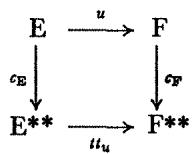
\includegraphics[keepaspectratio]{images/part002_cca49df6.jpg}}

是可交换的，这直接从定义和给出线性映射转置的公式(15)得出。

命题13. 若E是自由模（相应地，具有有限基的自由模），则典范映射 \(c_{E}:E \rightarrow E^{**}\) 是单射（相应地，双射）。

设 \((e_t)_{t \in \mathbb{T}}\) 是 \(\mathbf{E}\) 的一组基，并设 \((e_t^*)\) 为相应的坐标形式的族；根据定义，如果 \(x \in \mathbf{E}\) 满足 \(\tilde{x} = 0\) ，则 \(\langle x, e_t^* \rangle = 0\) 对所有 \(t \in \mathbb{T}\) 成立，换言之，即 \(x\) 的所有坐标均为零，因此 \(x = 0\) 。进一步假设 \(\mathbf{T}\) 是有限的；由于 \(\langle \tilde{e}_t, e_{t'}^* \rangle = \delta_{tt'}\) ， \((\tilde{e}_t)\) 是 \((e_t^*)\) 在 \(\mathbf{E}^{**}\) 中的对偶基，并且，由于 \(c_{\mathbf{E}}\) 把 \(\mathbf{E}\) 的一个基变换为 \(\mathbf{E}^{**}\) 的一个基， \(c_{\mathbf{E}}\) 是双射（§ 1，第 11 号，命题 17 的推论 3）。我们还证明了：

推论1. 设E是具有有限基的自由A-模；对于E的每个基 \((e_t)\) ， \((c_{\mathbf{E}}(e_t))\) 是 \((e_t^*)\) （E*的、与 \((e_t)\) 对偶的基）的对偶基。

在这种情况下，称 \((e_t)\) 和 \((e_t^*)\) 是彼此的对偶基。

推论2. 若E是具有有限基的自由A-模，则 \(\mathbf{E}^*\) 的每个有限基都是 \(\mathbf{E}\) 的某个基的对偶基。

只需考虑E**中给定基的对偶基，并将E典范地等同于E**即可。

推论3. 设E、F为两个均具有有限基的A-模，E（相应地，F）被典范地等同于其双重对偶E**（相应地，F**）。则对每个线性映射 \(u: \mathbf{E} \to \mathbf{F}\) ， \(^{tt}u = u\) 。

这直接从图表(27)的交换性得出。

推论4. 若P是投射模（相应地，有限生成投射模），则典范映射 \(c_{\mathbf{P}}: \mathbf{P} \to \mathbf{P}^{**}\) 是单射（相应地，双射）。

我们使用以下引理：

引理1. 设M、N是A-模E中的两个互补子模，i: M → E，j: N → E为典范单射。则图表

\begin{enumerate}
\def\labelenumi{(\arabic{enumi})}
\setcounter{enumi}{27}
\tightlist
\item
\end{enumerate}

\pandocbounded{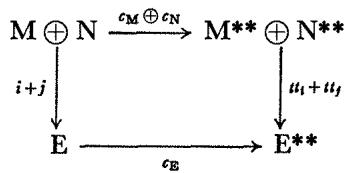
\includegraphics[keepaspectratio]{images/part002_690a791a.jpg}}

是交换的。

根据定义，对于 \(x \in \mathbf{M}\) , \(y \in \mathbf{N}\) , \(z^{*} \in \mathbf{E}^{*}\) ,

\[
\begin{array}{r l} \langle c _ {\mathrm{E}} (i (x) + j (y)), z ^ {*} \rangle & = \langle i (x) + j (y), z ^ {*} \rangle \\ & = \langle i (x), z ^ {*} \rangle + \langle j (y), z ^ {*} \rangle \\ & = \langle x, ^ {t} i (z ^ {*}) \rangle + \langle y, ^ {t} j (z ^ {*}) \rangle \\ & = \langle c _ {\mathrm{M}} (x), ^ {t} i (z ^ {*}) \rangle + \langle c _ {\mathrm{N}} (y), ^ {t} j (z ^ {*}) \rangle \\ & = \langle^ {t t} i (c _ {\mathrm{M}} (x)) + ^ {t t} j (c _ {\mathrm{N}} (y)), z ^ {*} \rangle . \end{array}
\]

既然如此，若E是自由模（相应地，具有有限基的自由模）， \(c_{E}\) 是单射（相应地，双射）；另一方面，由第6号、命题10可知， \(^{tt}i \oplus ^{tt}j\) 是双射的；图表(28)的交换性因此蕴含 \(c_{M} \oplus c_{N}\) 是单射（相应地，双射），因此 \(c_{M}\) 和 \(c_{N}\) （§1，第6号，命题7的推论1）亦然；考虑到第2号命题4，即得出推论。

\subsection{线性方程}

设 E、F 为两个 A-模。形如 \(u(x) = y_{0}\) 的每个方程（其中 \(u: E \to F\) 是一个给定的线性映射， \(y_{0}\) 是F的一个给定元素，而未知量x满足其取值在E中的条件）称为线性方程； \(y_{0}\) 称为方程的右端；如果 \(y_{0} = 0\) ，则方程称为齐次线性方程。

每个元素 \(x_{0} \in E\) ，若它满足 \(u(x_{0}) = y_{0}\) ，则称为线性方程 \(u(x) = y_{0}\) 的解。†

通常粗略地说，如果一个问题的求解等价于确定某个线性方程的解，那么这个问题就是线性的。

给定线性方程 \(u(x) = y_{0}\) ，方程 \(u(x) = 0\) 称为与 \(u(x) = y_{0}\) 相伴的齐次线性方程。

命题14. 若 \(x_{0}\) 是线性方程 \(u(x) = y_{0}\) 的一个解，则该方程的解集等于诸元素 \(x_{0} + z\) 的集合，其中 z 遍历相伴的齐次方程 \(u(x) = 0\) 的解集。

关系 \(u(x) = y_0\) 可以写成 \(u(x) = u(x_0)\) ，它等价于 \(u(x - x_0) = 0\) 。

换句话说，如果方程 \(u(x) = y_{0}\) 至少有一个解 \(x_{0}\) ，其解集就是集合 \(x_{0} + u^{-1}(0)\) ，它是由 u 的核 \(u^{-1}(0)\) 经平移得到的。注意， \(u^{-1}(0)\) 作为一个子模，永远不会是空的，因为它包含 0（称为齐次方程 \(u(x) = 0\) 的零解或平凡解）。

根据命题14，为使线性方程 \(u(x) = y_0\) 恰有一个解，必要且充分的是它至少有一个解，且 \(u^{-1}(0) = \{0\}\) （换句话说，即相伴的齐次方程没有非零解，或者说 \(u\) 是单射）；在这种情况下，对所有 \(y \in F\) ，方程 \(u(x) = y\) 至多有一个解。

命题15. 设 \(u\) 是模 \(\mathbf{E}\) 到模 \(\mathbf{F}\) 的一个线性映射。若方程 \(u(x) = y_0\) 至少有一个解，则 \(y_0\) 正交于 \(^t u\) 的核。

说 \(u(x) = y_{0}\) 有解意味着 \(y_{0} \in u(\mathbf{E})\) ，且该命题由第5号命题8的推论得出。

注意，命题15所给出的、方程 \(u(x) = y_{0}\) 有解的必要判据，当A是域时是充分的（§7，第6号，命题12），但一般不然（习题10）。

注记。(1) 设E是一个A-模， \((\mathbf{F}_{i})_{i\in I}\) 是一族A-模，并且对所有 \(i\in I\) ，设 \(u_{i}:E\to F_{i}\) 是一个线性映射。每个线性方程组

\[
u _ {i} (x) = y _ {i} \quad (i \in I)\tag{29}
\]

其中 \(y_{i} \in \mathbf{F}_{i}\) 是给定的，等价于单个线性方程 \(u(x) = y\) ，其中 \(u\) 是映射 \(x \mapsto (u_{i}(x))\) （从 \(\mathbf{E}\) 到 \(\mathbf{F} = \prod_{i \in I} \mathbf{F}_{i}\) ），而 \(y = (y_{i})\) 。方程组(29)称为齐次的，如果 \(y_{i} = 0\) 对所有 \(i \in I\) 成立。

\begin{enumerate}
\def\labelenumi{(\arabic{enumi})}
\setcounter{enumi}{1}
\tightlist
\item
  假设E有一个基 \((a_{\lambda})_{\lambda \in L}\) ；如果设 \(u(a_{\lambda}) = b_{\lambda}\) 对所有 \(\lambda \in L\) 成立，那么说 \(x = \sum_{\lambda \in L} \xi_{\lambda} a_{\lambda}\) 满足方程 \(u(x) = y_0\) ，就等价于说A中元素的（有限支撑的）族 \((\xi_{\lambda})_{\lambda \in L}\) 满足关系
\end{enumerate}

\[
\sum_ {\lambda \in L} \xi_ {\lambda} b _ {\lambda} = y _ {0}.\tag{30}
\]

反之，寻找A中元素的满足(30)的有限支撑的族 \((\xi_{\lambda})_{\lambda \in L}\) ，等价于求解线性方程 \(u(x) = y_0\) ，其中 \(u\) 是从 E 到 F 的唯一的线性映射，使得 \(u(a_{\lambda}) = b_{\lambda}\) 对所有 \(\lambda \in L\) 成立（§1，第 11 号，命题 17 的推论 3）。

\begin{enumerate}
\def\labelenumi{(\arabic{enumi})}
\setcounter{enumi}{2}
\tightlist
\item
  线性方程 \(u(x) = y_0\) 称为标量的，当 \(F = A_s\) ，从而 \(u\) 是 \(E\) 上的线性形式且 \(y_0\) 是标量时。若 \(E\) 有一组基 \((a_\lambda)_{\lambda \in L}\) ，则由注记（2）可知，这样的方程也可写成
\end{enumerate}

\[
\sum_ {\lambda \in L} \xi_ {\lambda} \alpha_ {\lambda} = y _ {0} \in A\tag{31}
\]

其中标量族 \((\alpha_{\lambda})\) 是任意的，并且约定该族 \((\xi_{\lambda})\) 必须具有有限支撑。一般地，标量线性方程组

\[
\sum_ {\lambda \in L} \xi_ {\lambda} \alpha_ {\lambda i} = \eta_ {i} \quad (i \in I)\tag{32}
\]

其中 \(\alpha_{\lambda i} \in A\) 且 \(\eta_i \in A\) ，其（A中的）解指的是一个有限支撑的族 \((\xi_\lambda)_{\lambda \in L}\) （由 \(A\) 中的元素组成），且满足(32)； \(\alpha_{\lambda i}\) 称为方程组的系数， \(\eta_i\) 称为右端项。这样的方程组的求解等价于方程 \(u(x) = y\) ，其中 \(y = (\eta_i)\) ，而 \(u: A_s^{(L)} \to A_s^I\) 是线性映射

\[
\left(\xi_ {\lambda}\right) \mapsto \left(\sum_ {\lambda \in L} \xi_ {\lambda} \alpha_ {\lambda i}\right).
\]

\begin{enumerate}
\def\labelenumi{(\arabic{enumi})}
\setcounter{enumi}{3}
\tightlist
\item
  线性方程组(32)在需要避免混淆时也称为左标量线性方程组。一个方程组
\end{enumerate}

\[
\sum_ {\lambda \in L} \alpha_ {\lambda i} \xi_ {\lambda} = \eta_ {i} \quad (i \in I)\tag{33}
\]

同样称为右标量线性方程组；把 \(\xi_{\lambda}, \eta_{i}\) 和 \(\alpha_{\lambda i}\) 视为属于A的相反环 A \(^{0}\) ，这样的方程组便可立即转化为方程组(32)。

\section{张量积}

\subsection{两个模的张量积}

设 \(G_{1}, G_{2}\) 为两个 Z-模；从集合 \(G = G_{1} \times G_{2}\) 到某个 Z-模的映射 u 称为双加性的（或 Z-双线性的），如果 \(u(x_{1}, x_{2})\) 关于 \(x_{1}\) 和关于 \(x_{2}\) 都是“加性的”；确切地说，这意味着，对于 \(x_{1}, y_{1}\) 在 \(G_{1}, x_{2}, y_{2}\) 在 \(G_{2}\) ，

\[
\begin{array}{l} u (x _ {1} + y _ {1}, x _ {2}) = u (x _ {1}, x _ {2}) + u (y _ {1}, x _ {2}) \\ u (x _ {1}, x _ {2} + y _ {2}) = u (x _ {1}, x _ {2}) + u (x _ {1}, y _ {2}). \end{array}
\]

注意这特别蕴含 \(u(0, x_2) = u(x_1, 0) = 0\) 对所有 \(x_1 \in \mathbf{G}_1, x_2 \in \mathbf{G}_2\) 成立。

设 A 为一个环，E 为一个右 A-模，F 为一个左 A-模。我们将考虑如下泛映射问题（集合论，IV，§ 3，第 1 号），其中 \(\Sigma\) 为 Z-模结构的类（此时态射即为 Z-线性映射，换言之，加法群同态），而 \(\alpha\) -映射是映射 \(f\) （从 E \(\times\) F 到某个 Z-模 G ），它们是 Z-双线性的，并且进一步满足：对所有 \(x \in \mathbf{E}\) , \(y \in \mathbf{F}\) 和 \(\lambda \in \mathbf{A}\)

\[
f (x \lambda , y) = f (x, \lambda y).\tag{1}
\]

我们证明该问题有解。为此，我们考虑Z-模 \(C = \mathbf{Z}^{(E \times F)}\) ，即由 \(E \times F\) 的元素以Z中为系数的形式线性组合所构成的Z-模（§1，第11号），其一组基可视为由有序对 \((x, y)\) （其中 \(x \in E\) ， \(y \in F\) ）组成。设D为C的子Z-模，由以下类型的元素生成：

\[
\left\{ \begin{array}{l} (x _ {1} + x _ {2}, y) - (x _ {1}, y) - (x _ {2}, y) \\ (x, y _ {1} + y _ {2}) - (x, y _ {1}) - (x, y _ {2}) \\ (x \lambda , y) - (x, \lambda y) \end{array} \right.\tag{2}
\]

其中 \(x, x_{1}, x_{2}\) 属于E， \(y, y_{1}, y_{2}\) 属于F，且 \(\lambda\) 属于A。

定义1. 右A-模E与左A-模F的张量积，记为 \(\mathbf{E} \otimes_{\mathbf{A}} \mathbf{F}\) 或 \(\mathbf{E} \otimes_{\mathbf{A}} \mathbf{F}\) （若不致引起混淆，也简记为 \(\mathbf{E} \otimes \mathbf{F}\) ），指的是商 \(\mathbf{Z}\) -模 C/D（即 \(\mathbf{Z}\) -模 C——由 \(\mathbf{E} \times \mathbf{F}\) 的元素以 \(\mathbf{Z}\) 中为系数的形式线性组合构成——除以由 (2) 中某一类型的元素所生成的子模 \(\mathbf{D}\) 而得的商）。对于 \(x \in \mathbf{E}\) 和 \(y \in \mathbf{F}\) ， \(\mathbf{E} \otimes_{\mathbf{A}} \mathbf{F}\) 中作为元素 \((x, y)\) （属于 \(\mathbf{C} = \mathbf{Z}^{(\mathbf{E} \times \mathbf{F})}\) ）的典范像的那个元素记为 \(x \otimes y\) ，并称为 \(x\) 与 \(y\) 的张量积。

映射 \((x,y)\mapsto x\otimes y\) 于 \(\mathbf{E}\times \mathbf{F}\) 到 \(\mathbf{E}\otimes_{\mathbf{A}}\mathbf{F}\) 称为典范的。它是一个满足条件(1)的Z-双线性映射。

我们证明张量积 \(E \otimes_{A} F\) 并且上述典范映射构成了先前提出的泛映射问题的一个解。确切地说：

命题1. (a) 设 \(g\) 是一个 \(\mathbf{Z}\) -线性映射（从 \(\mathbf{E} \otimes_{\mathbf{A}} \mathbf{F}\) 到某个 \(\mathbf{Z}\) -模 \(\mathbf{G}\) ）。映射 \((x, y) \mapsto f(x, y) = g(x \otimes y)\) （从 \(\mathbf{E} \times \mathbf{F}\) 到 \(\mathbf{G}\) ）是 \(\mathbf{Z}\) -双线性的，且满足条件(1)。

\begin{enumerate}
\def\labelenumi{(\alph{enumi})}
\setcounter{enumi}{1}
\tightlist
\item
  反之，设 \(f\) 是一个 \(\mathbf{Z}\) -双线性映射（从 \(\mathbf{E} \times \mathbf{F}\) 到某个 \(\mathbf{Z}\) -模 \(\mathbf{G}\) ），它满足条件(1)。则存在且仅存在一个 \(\mathbf{Z}\) -线性映射 \(g\) （从 \(\mathbf{E} \otimes_{\mathbf{A}} \mathbf{F}\) 到 \(\mathbf{G}\) ），使得 \(f(x,y) = g(x \otimes y)\) 对所有 \(x \in \mathbf{E}, y \in \mathbf{F}\) 成立。
\end{enumerate}

若 \(\phi\) 表示 \(\mathbf{E} \times \mathbf{F}\) 到 \(\mathbf{E} \otimes_{\mathbf{A}} \mathbf{F}\) 的典范映射，则 \(f = g \circ \phi\) ；由此得(a)。为证明(b)，我们注意到，在定义1的记号下， \(f\) 可延拓为一个 \(\mathbf{Z}\) -线性映射 \(\bar{f}\) （从 \(\mathbf{C}\) 到 \(\mathbf{G}\) ）（ \(\S 1\) ，第11号，命题17）。根据关系式(1)， \(\bar{f}\) 在 \(\mathbf{C}\) 的 (2) 中某一类型的所有元素上均为零，从而在 \(\mathbf{D}\) 上为零。因此存在一个 \(\mathbf{Z}\) -线性映射 \(g\) （从 \(\mathbf{C} / \mathbf{D} = \mathbf{E} \otimes_{\mathbf{A}} \mathbf{F}\) 到 \(\mathbf{G}\) ），使得 \(\bar{f} = g \circ \psi\) ，其中 \(\psi: \mathbf{C} \to \mathbf{C} / \mathbf{D}\) 是典范同态（ \(\S 1\) ，第8号，注记）。 \(g\) 的唯一性是直接的，因为 \(\mathbf{E} \otimes_{\mathbf{A}} \mathbf{F}\) 作为 \(\mathbf{Z}\) -模由形如 \(x \otimes y\) 的元素生成。

命题1定义了一个典范同构，它把E × F到G的、满足条件(1)的Z-双线性映射f所成的Z-模映到Z-模Hom \(_{Z}\) (E ⊗A F, G)上。

当 A = Z 时，条件 (1) 对每个 Z-双线性映射 f 自动满足，且 C 的子模 D 已由 (2) 中前两类元素生成。

现在我们回到一般情形，并且 \(E'\) 和 \(F'\) 分别表示E和F的底层Z-模，上述注记和定义1立即表明该Z-模 \(E \otimes_{A} F\) 可以典范地等同于 Z-模 \(E' \otimes_{Z} F'\) 的商模，该商模由形如 \((x\lambda) \otimes y - x \otimes (\lambda y)\) 的元素生成的子 Z-模所决定，其中 x 遍历 E，y 遍历 F，且 \(\lambda\) 遍历A。

推论1. 设H是一个Z-模，且 \(h:E \times F \rightarrow H\) 是一个满足条件(1)的Z-双线性映射，使得H由 \(h(E \times F)\) 生成。假设对于每个Z-模G以及每个从 \(E \times F\) 到G的满足(1)的Z-双线性映射f，

都存在一个Z-线性映射 \(g:H \to G\) ，使得 \(f = g \circ h\) 。那么，若 \(\phi\) 表示 \(E \times F\) 到 \(E \otimes_{A} F\) 的典范映射，则存在且仅存在一个同构 \(\theta\) （从 \(E \otimes_{A} F\) 到H上），使得 \(h = \theta \circ \phi\) 。

假设 \(h(\mathbf{E} \times \mathbf{F})\) 生成 H 蕴含了 g 的唯一性；该推论不过是泛映射问题解的一般唯一性性质（集合论，IV，§ 3，第 1 号）。

推论2. 设 \(\mathbf{E}^0\) （相应地 \(\mathbf{F}^0\) ）表示模 \(\mathbf{E}\) （相应地 \(\mathbf{F}\) ）被视为相反环 \(\mathbf{A}^0\) 上的左（相应地，右）模；则存在且仅存在一个 \(\mathbf{Z}\) -模同构 \(\sigma: \mathbf{E} \otimes_{\mathbf{A}} \mathbf{F} \to \mathbf{F}^0 \otimes_{\mathbf{A}^0} \mathbf{E}^0\) ，使得 \(\sigma(x \otimes y) = y \otimes x\) 对所有 \(x \in \mathbf{E}\) 和 \(y \in \mathbf{F}\) 成立（张量积的“交换性”）。

根据 \(A^{0}\) -模结构（在 \(E^{0}\) 和 \(F^{0}\) 上）的定义，映射 \((x,y)\mapsto y\otimes x\) （从 \(E\times F\) 到 \(F^{0}\otimes_{A^{0}}E^{0}\) ）是Z-双线性的且满足条件(1)，由此得到Z-线性映射 \(\sigma\) 的存在性和唯一性。类似地，可定义一个Z-线性映射 \(\tau:F^{0}\otimes_{A^{0}}E^{0}\to E\otimes_{A}F\) 使得 \(\tau(y\otimes x)=x\otimes y\) ，并且显然 \(\sigma\) 和 \(\tau\) 是互逆的同构。

注记. 非零模的张量积可能为零：例如，取两个Z-模 E = Z/2Z 和 F = Z/3Z，则对所有 \(x \in E\) 和 \(y \in F\) 都有 2x = 0 和 3y = 0；因此，在 E \(\otimes_{\mathbf{Z}} F\) 中，

\[
x \otimes y = 3 (x \otimes y) - 2 (x \otimes y) = x \otimes (3 y) - (2 x) \otimes y = 0
\]

对所有 \(x\) 和 \(y\) 成立（参见第6号，命题6的推论4）。

\subsection{两个线性映射的张量积}

设A是一个环，E、E'是两个右A-模，F、F'是两个左A-模，且 \(u: E \rightarrow E'\) 和 \(v: F \rightarrow F'\) 是两个A-线性映射。容易验证，映射

\[
(x, y) \mapsto u (x) \otimes v (y)
\]

（从 \(\mathbf{E} \times \mathbf{F}\) 到 \(\mathbf{E}' \otimes_{\mathbf{A}} \mathbf{F}'\) ）是 \(\mathbf{Z}\) -双线性的，且满足第1号的条件(1)。因此，根据第1号命题1，存在且仅存在一个 \(\mathbf{Z}\) -线性映射 \(w: \mathbf{E} \otimes_{\mathbf{A}} \mathbf{F} \to \mathbf{E}' \otimes_{\mathbf{A}} \mathbf{F}'\) ，使得

\[
w (x \otimes y) = u (x) \otimes v (y)\tag{3}
\]

对于 \(x \in \mathbf{E}\) ， \(y \in \mathbf{F}\) 。此映射记作 \(u \otimes v\) （当不致引起混淆时），并称为线性映射 \(u\) 与 \(v\) 的张量积。

由(3)立即得出 \((u, v) \mapsto u \otimes v\) 是一个Z-双线性映射，称为典范映射

\[
\operatorname{Hom} _ {\mathbf {A}} (\mathrm{E}, \mathrm{E} ^ {\prime}) \times \operatorname{Hom} _ {\mathbf {A}} (\mathrm{F}, \mathrm{F} ^ {\prime}) \rightarrow \operatorname{Hom} _ {\mathbf {Z}} (\mathrm{E} \otimes_ {\mathbf {A}} \mathrm{F}, \mathrm{E} ^ {\prime} \otimes_ {\mathbf {A}} \mathrm{F} ^ {\prime}).
\]

根据第1号命题1，与之对应的是一个 \(\mathbf{Z}\) -线性映射，称为典范映射

\[
\operatorname{Hom} _ {\mathbf {A}} (\mathrm{E}, \mathrm{E} ^ {\prime}) \otimes_ {\mathbf {Z}} \operatorname{Hom} _ {\mathbf {A}} (\mathrm{F}, \mathrm{F} ^ {\prime}) \rightarrow \operatorname{Hom} _ {\mathbf {Z}} (\mathrm{E} \otimes_ {\mathbf {A}} \mathrm{F}, \mathrm{E} ^ {\prime} \otimes_ {\mathbf {A}} \mathrm{F} ^ {\prime})\tag{4}
\]

它把张量积的每个元素 \(u \otimes v\) 对应到线性映射 \(u \otimes v: \mathbf{E} \otimes_{\mathbf{A}} \mathbf{F} \to \mathbf{E}' \otimes_{\mathbf{A}} \mathbf{F}'\) 。注意，典范映射(4)不一定是单射的，也不一定是满射的。因此记号 \(u \otimes v\) 可能引起混淆，须由上下文指明它表示的是张量积的元素还是线性映射。

此外，设 \(\mathbf{E}''\) 是一个右A-模， \(\mathbf{F}''\) 是一个左A-模，且 \(u':\mathbf{E}'\to\mathbf{E}''\) , \(v':\mathbf{F}'\to\mathbf{F}''\) 是A-线性映射；由(3)得出

\[
\left(u ^ {\prime} \circ u\right) \otimes \left(v ^ {\prime} \circ v\right) = \left(u ^ {\prime} \otimes v ^ {\prime}\right) \circ (u \otimes v).\tag{5}
\]
% semantic-fragments: legacy-input-seam
\relax{}
\subsection{环的更换}

命题2. 设 A、B 为两个环， \(\rho: \mathbf{B} \to \mathbf{A}\) 为一个环同态，且 E（相应地，F）为右（相应地，左）A-模。则存在且仅存在一个 Z-线性映射

\[
\phi : \rho_ {*} (\mathbf {E}) \otimes_ {\mathbf {B}} \rho_ {*} (\mathbf {F}) \rightarrow \mathbf {E} \otimes_ {\mathbf {A}} \mathbf {F}\tag{6}
\]

使得对所有 \(x \in \mathbf{E}\) 与 \(y \in \mathbf{F}\) ， \(\phi\) 在元素 \(x \otimes y\) （它属于 \(\rho_{*}(\mathbf{E}) \otimes_{\mathbf{B}} \rho_{*}(\mathbf{F})\) ）处的像是元素 \(x \otimes y\) （它属于 \(\mathbf{E} \otimes_{\mathbf{A}} \mathbf{F}\) ） ；这个 \(\mathbf{Z}\) -线性映射是满射的。

我们考虑映射 \((x,y)\mapsto x\otimes y\) ，即从 \(\rho_{\star}(E)\times \rho_{*}(F)\) 到 \(E\otimes_A F\) 的映射；它是 Z-双线性的，并且对所有 \(\beta \in B\) ，根据定义有 \((x\rho (\beta))\otimes y = x\otimes (\rho (\beta)y)\) ，因此第1号的条件 (1) 成立，从而得到 \(\phi\) 的存在性与唯一性（第1号，命题1）。后一断言由元素 \(x\otimes y\) 生成 Z-模 \(E\otimes_A F\) 这一事实得出。

映射 (6) 称为典范映射。

推论。设 \(\mathfrak{a}\) 是A的一个双边理想，使得 \(\mathfrak{a}\) 包含于 E 的零化子与 F 的零化子中，从而 E（相应地 F）具有典范的左（相应地右） \((A/\mathfrak{a})\)-模结构（§ 1，第 12 号）。于是典范同态 (6)

\[
\phi : \mathbf {E} \otimes_ {\mathbf {A}} \mathbf {F} \rightarrow \mathbf {E} \otimes_ {\mathbf {A} / \mathfrak {a}} \mathbf {F}
\]

对应于典范同态 \(\rho: \mathbf{A} \to \mathbf{A} / \mathfrak{a}\) 是恒等映射。

对所有 \(\bar{\alpha} \in \mathbf{A} / \mathfrak{a}\) 、所有 \(x \in \mathbf{E}\) 以及所有 \(y \in \mathbf{F}\) ，有 \(x\bar{\alpha} = x\alpha\) （相应地， \(\bar{\alpha}y = \alpha y\) ），其中 \(\alpha\) 取遍满足 \(\rho(\alpha) = \bar{\alpha}\) 的一切元素。若 \(\mathbf{C} = \mathbf{Z}^{(\mathbb{E} \times \mathbb{F})}\) ，则 \(\mathbf{C}\) 中由元素 \((x\alpha, y) - (x, \alpha y)\) 生成的子模等于由元素 \((x\bar{\alpha}, y) - (x, \bar{\alpha}y)\) 生成的子模。

在命题2的假设和记号下，设 \(\mathbf{E}'\) 是一个右B-模， \(\mathbf{F}'\) 一个左B-模，并考虑两个半线性映射 \(u: \mathbf{E}' \to \mathbf{E}\) , \(v: \mathrm{F}' \to \mathrm{F}\) （它们相对于同态 \(\rho: \mathrm{B} \to \mathrm{A}\) ）； \(u\) （相应地 \(v\) ) 可被视为一个 B-线性映射 \(\mathrm{E}' \to \rho_*(\mathrm{E})\) （相应地 \(\mathrm{F}' \to \rho_*(\mathrm{F})\) )，从而得到一个 Z-线性映射 \(w: \mathrm{E}' \otimes_{\mathrm{B}} \mathrm{F}' \to \rho_*(\mathrm{E}) \otimes_{\mathrm{B}} \rho_*(\mathrm{F})\) ，使得 \(w(x' \otimes y') = u(x') \otimes v(y')\) ，其中 \(x' \in \mathrm{E}', y' \in \mathrm{F}'\) ；将典范映射 (6) 与这个映射复合，便得到一个 Z-线性映射 \(w': \mathrm{E}' \otimes_{\mathrm{B}} \mathrm{F}' \to \mathrm{E} \otimes_{\mathrm{A}} \mathrm{F}\) ，使得 \(w'(x' \otimes y') = u(x') \otimes v(y')\) ，其中 \(x' \in \mathrm{E}', y' \in \mathrm{F}'\) ；若不致引起混淆，这个映射通常就记作 \(u \otimes v\) 。显然， \((u, v) \mapsto u \otimes v\) 是一个 Z-双线性映射

\[
\operatorname{Hom} _ {\mathbf {B}} \left(\mathrm{E} ^ {\prime}, \rho_ {*} (\mathrm{E})\right) \times \operatorname{Hom} _ {\mathbf {B}} \left(\mathrm{F} ^ {\prime}, \rho_ {*} (\mathrm{F})\right)\rightarrow \operatorname{Hom} _ {\mathbf {Z}} \left(\mathrm{E} ^ {\prime} \otimes_ {\mathbf {B}} \mathrm{F} ^ {\prime}, \mathrm{E} \otimes_ {\mathbf {A}} \mathrm{F}\right).
\]

此外，若 C 是第三个环， \(\sigma: \mathrm{C} \to \mathrm{B}\) 是一个同态， \(\mathrm{E}''\) 是一个右C-模， \(\mathrm{F}''\) 是一个左C-模， \(u': \mathrm{E}'' \to \mathrm{E}'\) 和 \(v': \mathrm{F}'' \to \mathrm{F}'\) 是相对于 \(\sigma\) 的半线性映射，则

\[
(u \circ u ^ {\prime}) \otimes (v \circ v ^ {\prime}) = (u \otimes v) \circ (u ^ {\prime} \otimes v ^ {\prime}).
\]

\subsection{张量积上的算子；张量积作为多重模}

在第1号的假设和记号下，对于每个自同态 \(u\) （相应地 \(v\) ，即 A-模 \(E\) （相应地 \(F\) ) 的自同态）， \(u \otimes l_F\) （相应地 \(l_E \otimes v\) ）是 \(Z\) -模 \(E \otimes_A F\) 的自同态；由第2号的公式 (5) 立即得出，映射 \(u \mapsto u \otimes l_F\) （相应地 \(v \mapsto l_E \otimes v\) ）是一个环同态

\[
\operatorname{End} _ {\mathbf {A}} (\mathbf {E}) \rightarrow \operatorname{End} _ {\mathbf {Z}} (\mathbf {E} \otimes_ {\mathbf {A}} \mathbf {F})
\]

（相应地 \(\operatorname{End}_{\mathbf{A}}(\mathbf{F}) \to \operatorname{End}_{\mathbf{Z}}(\mathbf{E} \otimes_{\mathbf{A}} \mathbf{F}))\) ；此外，

\[
(u \otimes \mathrm{l} _ {\mathrm{F}}) \circ (\mathrm{l} _ {\mathrm{E}} \otimes v) = (\mathrm{l} _ {\mathrm{E}} \otimes v) \circ (u \otimes \mathrm{l} _ {\mathrm{F}}) = u \otimes v\tag{7}
\]

因此（§ 1，第 14 号） E ⊗\_A F 关于环 End\_A(E) 与 End\_A(F) 具有典范的双模结构。

既然如此，假设在 E 上给定一个 \(((\mathbf{B}_i^{\prime});\mathbf{A},(\mathbf{C}_j^{\prime}))\) -多重模结构，在 F 上给定一个 \((\mathbf{A},(\mathbf{B}_h^{\prime});(\mathbf{C}_k^{\prime}))\) -多重模结构（§ 1，第 14 号）；这等同于说，给定了环同态 \(\mathrm{B}_i^\prime \to \mathrm{End}_{\mathbf{A}}(\mathbf{E})\) , \(\mathrm{C}_j^{\prime 0} \to \mathrm{End}_{\mathbf{A}}(\mathbf{E})\) ，其像两两可交换，以及环同态 \(\mathrm{B}_h^{\prime \prime} \to \mathrm{End}_{\mathbf{A}}(\mathbf{F})\) , \(\mathrm{C}_k^{\prime \prime 0} \to \mathrm{End}_{\mathbf{A}}(\mathbf{F})\) ，其像也两两可交换。若将这些同态分别与上面定义的典范同态 \(\mathrm{End}_{\mathbf{A}}(\mathbf{E}) \to \mathrm{End}_{\mathbf{Z}}(\mathbf{E} \otimes_{\mathbf{A}} \mathbf{F})\) 和 \(\mathrm{End}_{\mathbf{A}}(\mathbf{F}) \to \mathrm{End}_{\mathbf{Z}}(\mathbf{E} \otimes_{\mathbf{A}} \mathbf{F})\) 复合，则（考虑到 (7)）可以看出，环同态

\[
\mathrm{B} _ {i} ^ {\prime} \rightarrow \operatorname{End} _ {\mathbf {Z}} (\mathrm{E} \otimes_ {\mathrm{A}} \mathrm{F}), \quad \mathrm{C} _ {j} ^ {\prime 0} \rightarrow \operatorname{End} _ {\mathbf {Z}} (\mathrm{E} \otimes_ {\mathrm{A}} \mathrm{F})
\]

\[
\mathrm{B} _ {h} ^ {\prime \prime} \rightarrow \operatorname{End} _ {\mathbf {Z}} (\mathrm{E} \otimes_ {\mathrm{A}} \mathrm{F}), \quad \mathrm{C} _ {k} ^ {\prime \prime 0} \rightarrow \operatorname{End} _ {\mathbf {Z}} (\mathrm{E} \otimes_ {\mathrm{A}} \mathrm{F})
\]

其像两两可交换；换句话说，在 \(\mathbf{E} \otimes_{\mathbf{A}} \mathbf{F}\) 上定义了一个 \(((\mathbf{B}_i'), (\mathbf{B}_h''); (\mathbf{C}_j'), (\mathbf{C}_k'')\) -多重模结构；正是这个多重模也称为 \(((\mathbf{B}_i^{\prime});\mathbf{A},(\mathbf{C}_j^{\prime}))\) -多重模 E 与 \((\mathbf{A},(\mathbf{B}_h^{\prime\prime});(\mathbf{C}_k^{\prime\prime}))\) -多重模 F 的（相对于 A 的）张量积。这个多重模是类似于第1号中所考虑的泛映射问题的解；确切地说：

命题3. 设 G 为 \(((\mathbf{B}_i'), (\mathbf{B}_h''); (\mathbf{C}_j'), (\mathbf{C}_k''))-multimodule.\) 。

\begin{enumerate}
\def\labelenumi{(\alph{enumi})}
\tightlist
\item
  设 \(g\) 是多重模 \(\mathbf{E} \otimes_{\mathbf{A}} \mathbf{F}\) 到 \(\mathbf{G}\) 的一个线性映射。映射 \(f: (x, y) \mapsto g(x \otimes y)\) （从 \(\mathbf{E} \times \mathbf{F}\) 到 \(\mathbf{G}\) ）是 \(\mathbf{Z}\) -双线性的，且满足第1号的关系 (1) 以及条件
\end{enumerate}

\[
\left\{ \begin{array}{l l} f (\mu_ {i} ^ {\prime} x, y) = \mu_ {i} ^ {\prime} f (x, y), & f (x \nu_ {j} ^ {\prime}, y) = f (x, y) \nu_ {j} ^ {\prime} \\ f (x, \mu_ {h} ^ {\prime \prime} y) = \mu_ {h} ^ {\prime \prime} f (x, y), & f (x, y \nu_ {k} ^ {\prime \prime}) = f (x, y) \nu_ {k} ^ {\prime \prime} \end{array} \right.\tag{8}
\]

对所有 \(x \in \mathbf{E}, y \in \mathbf{F}\) , \(\mu_i' \in \mathbf{B}_i'\) , \(\nu_j' \in \mathbf{C}_j'\) , \(\mu_h'' \in \mathbf{B}_h''\) , \(\nu_k'' \in \mathbf{C}_{k}''\) 成立，其中 \(i, j, h, k\) 任意。

\begin{enumerate}
\def\labelenumi{(\alph{enumi})}
\setcounter{enumi}{1}
\tightlist
\item
  反之，设 \(f\) 是一个 \(\mathbf{Z}\) -双线性映射（从 \(\mathbf{E} \times \mathbf{F}\) 到 \(\mathbf{G}\) ），满足条件 (1)（第1号）和 (8)。则存在且仅存在一个线性映射 \(g\) （从多重模 \(\mathbf{E} \otimes_{\mathbf{A}} \mathbf{F}\) 到多重模 \(\mathbf{G}\) ），使得 \(f(x, y) = g(x \otimes y)\) ，其中 \(x \in \mathbf{E}, y \in \mathbf{F}\) 。
\end{enumerate}

断言 (a) 直接由 \(\mathbf{E} \otimes_{\mathbf{A}} \mathbf{F}\) 上多重模结构的定义得出，因为例如 \((x \otimes y)\nu_j' = (x\nu_j') \otimes y\) 。为证明 (b)，我们首先注意到，第1号的命题1给出了 \(\mathbf{Z}\) -线性映射 \(g\) 的存在性和唯一性，它满足 \(g(x \otimes y) = f(x, y)\) （其中 \(x \in \mathbf{E}\) , \(y \in \mathbf{F}\) ）；只需验证 \(g\) 关于多重模结构是线性的。由于元素 \(x \otimes y\) 生成 \(\mathbf{Z}\) -模 \(\mathbf{E} \otimes_{\mathbf{A}} \mathbf{F}\) ，只需验证关系 \(g(\mu'(x \otimes y)) = \mu_i' g(x \otimes y)\) 及其类似关系；但这由公式 \(g(x \otimes y) = f(x, y)\) 以及关系式 (8) 立即得出。

注释。\(\mathbf{E} \otimes_{\mathbf{A}} \mathbf{F}\) 的元素一般说来可以有多种方式写成 \(\sum_{i} (x_i \otimes y_i)\) 的形式，其中 \(x_i \in \mathbf{E}\) 且 \(y_i \in \mathbf{F}\) ；但要定义线性映射 \(g\) （从多重模 \(\mathbf{E} \otimes_{\mathbf{A}} \mathbf{F}\) 到一个多重模 \(\mathbf{G}\) ），无需验证：若 \(\sum_{i} (x_i \otimes y_i) = \sum_{j} (x_j' \otimes y_j')\) ，则 \(\sum_{i} g(x_i \otimes y_i) = \sum_{j} g(x_j' \otimes y_j')\) ；只需给定 \(g(x \otimes y)\) （对于 \(x \in \mathbf{E}\) 与 \(y \in \mathbf{F}\) ），并验证 \((x, y) \mapsto g(x \otimes y)\) 是 \(\mathbf{Z}\) -双线性的且满足条件 (1)（第1号）和 (8)。

设 \(\mathbf{E}'\) 是 \(((\mathbf{B}_i'),\mathbf{A},(\mathbf{C}_j')\) -多重模， \(\mathbf{F}'\) 一个 \((\mathbf{A},(\mathbf{B}_h'');(\mathbf{C}_k'')\) -多重模，且 \(u:\mathbf{E}\to \mathbf{E}',v:\mathbf{F}\to \mathbf{F}'\) 为多重模的线性映射；由定义（第2号）立即得出， \(u\otimes v\) 是从多重模 \(\mathbf{E}\otimes_{\mathbf{A}}\mathbf{F}\) 到多重模 \(\mathbf{E}'\otimes_{\mathbf{A}}\mathbf{F}'\) 的线性映射。

设 E 始终表示右 A-模，令 \(_{s}A_{d}\) 表示把环 A 视为 (A, A)-双模（ \(\S\) 1，第 14 号，例 1）；由上述可知，张量积 \(\mathbf{E} \otimes_{\mathbf{A}} (\mathbf{s}\mathbf{A}_{d})\) 具有典范的右 A-模结构，使得 \((x \otimes \lambda)\mu = x \otimes (\lambda\mu)\) ，其中 \(x \in E\) , \(\lambda \in A\) , \(\mu \in A\) 。映射 \((x, \lambda) \mapsto x\lambda\) （从 \(\mathbf{E} \times (\mathbf{s}\mathbf{A}_{d})\) 到 E ）是 Z-双线性的，并满足条件 (1)（第 1 号）和 (8)

（在后一种情形中， \(\mathbf{B}_i'\) , \(\mathbf{C}_j'\) 和 \(\mathbf{B}_h''\) 不出现，而族 \((\mathbf{C}_k'')\) 就化为 \(\mathbf{A}\) ）；因此（命题3），存在一个 A-线性映射 \(g\) （称为典范映射），它把 \(\mathbf{E} \otimes_{\mathbf{A}} (s\mathbf{A}_d)\) 映入 \(\mathbf{E}\) ，使得 \(g(x \otimes \lambda) = x\lambda\) ，其中 \(x \in \mathbf{E}\) , \(\lambda \in \mathbf{A}\) 。

命题4. 若 E 是一个右 A-模，则映射 \(h: x \mapsto x \otimes 1\) （它把 E 映入 \(\mathbf{E} \otimes_{\mathbf{A}} (s\mathbf{A}_d)\) ）是一个右 A-模同构，其逆同构 \(g\) 满足 \(g(x \otimes \lambda) = x\lambda\) ，其中 \(x \in \mathbf{E}, \lambda \in \mathbf{A}\) 。

若 \(g\) 是典范映射，则 \(g \circ h\) 是恒等映射 \(1_{\mathbf{E}}\) ，且 \(h \circ g\) 与 \(\mathbf{E} \otimes_{\mathbf{A}} (s\mathbf{A}_d)\) 到自身的恒等映射在形如 \(x \otimes y\) 的元素上一致，而这些元素生成这个 \(\mathbf{Z}\) -模；由此得出结论。

我们通常将写成 \(E \otimes_{A} A\) 而不是 \(E \otimes_{A} (s A_{d})\) ，并经常通过上述典范同构把 \(E \otimes_{A} A\) 与 E 等同。注意，若 E 还具有与其右 A-模结构相容的（左或右）B-模结构，则 g 和 h 对于 E 和 \(E \otimes_{A} A\) 上的 B-模结构也是同构（从而也是多重模同构）。

现在设 F 是一个左 A-模； \((sA_{d}) \otimes_{A} F\) （也记作 A \(\otimes_{A} F\) ）则具有典范的左 A-模结构，并且如同命题 4 那样，可定义一个从 A \(\otimes_{A} F\) 到 F 上的典范同构，它把 \(\lambda \otimes x\) 映为 \(\lambda x\) ，其逆同构为 \(x \mapsto 1 \otimes x\) 。

特别地，存在 (A, A)-双模 \((_{s}\mathbf{A}_{d})\otimes_{\mathbf{A}}(_{s}\mathbf{A}_{d})\) 到 \({}_{s}\mathbf{A}_{d}\) 上的一个典范同构，它把 \(\lambda \otimes \mu\) 映为 \(\lambda \mu\) 。

\subsection{交换环上两个模的张量积}

设 C 为一个交换环；对于每个 C-模 E，E 上的模结构与自身相容（§ 1，第 14 号）。若 E 和 F 是两个 C-模，则第 4 号的讨论使我们能够在张量积 E ⊗c F 上定义两个 C-模结构，分别使得 γ(x ⊗ y) = (γx) ⊗ y 以及 γ(x ⊗ y) = x ⊗ (γy)；但由于根据第 1 号定义 1，在此情形下 (γx) ⊗ y = x ⊗ (γy)，这两个结构是相同的。此后当我们把 E ⊗c F 作为 C-模来讨论时，除非另有说明，均指按此方式定义的结构。典范同构

\[
\sigma : \mathbf {F} \otimes_ {\mathbf {c}} \mathbf {E} \rightarrow \mathbf {E} \otimes_ {\mathbf {c}} \mathbf {F}
\]

（第 1 号，命题 1 的推论 2）则是一个 C-模同构。

由这一定义可知，若 \((a_{\lambda})_{\lambda\in\mathbb{L}}\) （相应地 \((b_{\mu})_{\mu\in\mathbb{M}}\) ）是 C-模 E（相应地 F）的一个生成系，则 \((a_{\lambda}\otimes b_{\mu})\) 是 C-模 \(E\otimes_{C}F\) 的一个生成系；特别地，若 E 和 F 是有限生成的 C-模，则 \(E\otimes_{C}F\) 亦然。

对于每个 C-模 G，那些 Z-双线性映射 \(f\) （从 \(\mathbf{E} \times \mathbf{F}\) 到 \(\mathbf{G}\) ），若它们满足

\[
f (\gamma x, y) = f (x, \gamma y) = \gamma f (x, y) \quad \text { for } x \in \mathbf {E}, y \in \mathbf {F}, \gamma \in \mathbf {C}\tag{9}
\]

于是称为 C-双线性映射，并构成一个 C-模，记作 \(\mathcal{L}_2(\mathrm{E},\mathrm{F};\mathrm{G})\) ；命题 3（第4号）定义了一个典范的 C-模同构（参见 §1，第 14 号，注记 1）。

\[
\mathcal {L} _ {2} (\mathrm{E}, \mathrm{F}; \mathrm{G}) \rightarrow \operatorname{Hom} _ {\mathbf {c}} (\mathrm{E} \otimes_ {\mathbf {c}} \mathrm{F}, \mathrm{G}).\tag{10}
\]

设 \(E'\) , \(F'\) 是两个 C-模，且 \(u: E \to E'\) , \(v: F \to F'\) 是两个 C-线性映射；则（第4号） \(u \otimes v\) 是 \(E \otimes_{\mathbb{C}} F\) 到 \(E' \otimes_{\mathbb{C}} F'\) 的 C-线性映射。进一步，立即可以看出 \((u, v) \mapsto u \otimes v\) 是 \(\operatorname{Hom}_{\mathbb{C}}(\mathbf{E}, \mathbf{E}') \times \operatorname{Hom}_{\mathbb{C}}(\mathbf{F}, \mathbf{F}')\) 到 \(\operatorname{Hom}_{\mathbb{C}}(\mathbf{E} \otimes_{\mathbb{C}} \mathbf{F}, \mathbf{E}' \otimes_{\mathbb{C}} \mathbf{F}')\) 的 C-双线性映射；因此典范地对应于它的一个 C-线性映射，称为典范映射：

\[
\operatorname{Hom} _ {\mathbf {c}} (\mathbf {E}, \mathbf {E} ^ {\prime}) \otimes_ {\mathbf {c}} \operatorname{Hom} _ {\mathbf {c}} (\mathbf {F}, \mathbf {F} ^ {\prime}) \to \operatorname{Hom} _ {\mathbf {c}} (\mathbf {E} \otimes_ {\mathbf {c}} \mathbf {F}, \mathbf {E} ^ {\prime} \otimes_ {\mathbf {c}} \mathbf {F} ^ {\prime})\tag{11}
\]

它使每个元素 \(u \otimes v\) （它属于张量积

\[
\operatorname{Hom} _ {\mathbf {c}} (\mathbf {E}, \mathbf {E} ^ {\prime}) \otimes_ {\mathbf {c}} \operatorname{Hom} _ {\mathbf {c}} (\mathbf {F}, \mathbf {F} ^ {\prime})
\]

）对应到线性映射 \(u \otimes v\) 。注意，典范映射（11）不一定是单射也不是满射（§4，习题2）。

注记. (1) 设 A, B 为两个交换环， \(\rho:B\to A\) 为一个环同态，且 E 与 F 为两个 A-模；则第 3 号中的典范映射 (6) 是一个 B-线性映射

\[
\rho_ {*} (\mathbf {E}) \otimes \rho_ {*} (\mathbf {F}) \rightarrow \rho_ {*} (\mathbf {E} \otimes_ {\mathbf {A}} \mathbf {F}).\tag{12}
\]

\begin{enumerate}
\def\labelenumi{(\arabic{enumi})}
\setcounter{enumi}{1}
\tightlist
\item
  本号中所述内容可推广到如下情形：设 E 为右 A-模，F 为左 A-模，C 为交换环，且 \(\rho:C\to A\) 为 C 到 A 的同态，使得 \(\rho(\mathbf{C})\) 包含在 A 的中心内（参见 III，§1，第 3 号）。于是我们可以考虑 C-模 \(\rho_{*}(\mathbf{E})\) 和 \(\rho_{*}(\mathbf{F})\) ，并且关于 \(\rho\) 的假设蕴含这些 C-模结构分别与 E 和 F 上的 A-模结构相容（§1，第 14 号）。张量积 \(E\otimes_{A}F\) 因此（根据第4号）被赋予两个 C-模结构，使得 \(\gamma(x\otimes y)=(x\rho(\gamma))\otimes y\) 和
\end{enumerate}

\[
\gamma (x \otimes y) = x \otimes (\rho (\gamma) y)
\]

分别对 \(\gamma\in\mathbf{C}\) , \(x\in\mathbf{E}\) , \(y\in\mathbf{F}\) 成立，并且定义 1（第 1 号）还表明这两个结构是相同的。若 \(\mathbf{E}'\) （相应地 \(\mathbf{F}'\) ）是一个右（相应地，左）A-模，且 \(u:\mathbf{E}\to\mathbf{E}'\) , \(v:\mathbf{F}\to\mathbf{F}'\) 是两个 A-线性映射，则 \(u\otimes v:\mathbf{E}\otimes_{\mathbf{A}}\mathbf{F}\to\mathbf{E}'\otimes_{\mathbf{A}}\mathbf{F}'\) 对于刚刚定义的 C-模结构而言是 C-线性的；映射 \((u,v)\mapsto u\otimes v\) :

\[
\operatorname{Hom} _ {\mathbf {A}} (\mathrm{E}, \mathrm{E} ^ {\prime}) \times \operatorname{Hom} _ {\mathbf {A}} (\mathrm{F}, \mathrm{F} ^ {\prime}) \rightarrow \operatorname{Hom} _ {\mathbf {C}} (\mathrm{E} \otimes_ {\mathbf {A}} \mathrm{F}, \mathrm{E} ^ {\prime} \otimes_ {\mathbf {A}} \mathrm{F} ^ {\prime})
\]

是 C-双线性的（对于 \(\mathrm{Hom}_{\mathbf{A}}(\mathbf{E},\mathbf{E}^{\prime})\) 和 \(\mathrm{Hom}_{\mathbf{A}}(\mathbf{F},\mathbf{F}^{\prime})\) 上的

在 §1，第 14 号，注记 1 中定义的 C-模结构），由此我们还导出一个 C-线性映射，称为典范映射

\[
\operatorname{Hom} _ {\mathbf {A}} (\mathbf {E}, \mathbf {E} ^ {\prime}) \otimes_ {\mathbf {C}} \operatorname{Hom} _ {\mathbf {A}} (\mathbf {F}, \mathbf {F} ^ {\prime}) \rightarrow \operatorname{Hom} _ {\mathbf {C}} (\mathbf {E} \otimes_ {\mathbf {A}} \mathbf {F}, \mathbf {E} ^ {\prime} \otimes_ {\mathbf {A}} \mathbf {F} ^ {\prime}).\tag{13}
\]

\begin{enumerate}
\def\labelenumi{(\arabic{enumi})}
\setcounter{enumi}{2}
\tightlist
\item
  设 \(\mathbf{A}\) 是一个整环， \(\mathbf{K}\) 为其分式域。若 \(\mathbf{E}\) 和 \(\mathbf{F}\) 是两个向量 \(\mathbf{K}\) -空间，则典范映射
\end{enumerate}

\[
\left(\mathbf {E} _ {[ \mathbf {A} ]}\right) \otimes_ {\mathbf {A}} \left(\mathbf {F} _ {[ \mathbf {A} ]}\right)\rightarrow \mathbf {E} \otimes_ {\mathbf {K}} \mathbf {F}
\]

（第 3 号及 §1，第 13 号）是双射的。只需（第4号）证明：若 \(f\) 是 \(\mathbf{E} \times \mathbf{F}\) 到向量 K-空间 \(\mathbf{G}\) 的一个 A-双线性映射，则 \(f\) 也是 K-双线性的。现在，对所有 \(\alpha \neq 0\) （在 \(\mathbf{A}\) 中）：

\[
\alpha f (\alpha^ {- 1} x, y) = f (x, y) = \alpha f (x, \alpha^ {- 1} y)
\]

，因此

\[
f (\alpha^ {- 1} x, y) = f (x, \alpha^ {- 1} y) = \alpha^ {- 1} f (x, y)
\]

，因为 G 是一个向量 K-空间。

\subsection{E ⊗\_A F 关于正合序列的性质}

命题5. 设 E、E'、E'' 为右 A-模，F 为左 A-模，且

\[
\mathrm{E} ^ {\prime} \stackrel {u} {\longrightarrow} \mathrm{E} \stackrel {v} {\longrightarrow} \mathrm{E} ^ {\prime \prime} \longrightarrow 0\tag{14}
\]

是线性映射的一个正合列。记 \(\bar{u} = u \otimes 1_{\mathbb{F}}, \bar{v} = v \otimes 1_{\mathbb{F}}\) ，则序列

\[
\mathrm{E} ^ {\prime} \otimes_ {\mathrm{A}} \mathrm{F} \xrightarrow {\bar {u}} \mathrm{E} \otimes_ {\mathrm{A}} \mathrm{F} \xrightarrow {\bar {v}} \mathrm{E} ^ {\prime \prime} \otimes_ {\mathrm{A}} \mathrm{F} \longrightarrow 0\tag{15}
\]

是 Z-同态组成的正合列。

根据第 2 号，公式（5）， \(\bar{v} \circ \bar{u} = (v \circ u) \otimes 1_{\mathbf{F}} = 0\) ；像 \(\mathrm{H} = \bar{u} (\mathbf{E}' \otimes \mathbf{F})\) 包含于核 \(\mathbf{L} = \operatorname{Ker}(\bar{v})\) ；通过取商，我们从 \(\bar{v}\) 得到一个 \(\mathbf{Z}\) -线性映射 \(f\) ，它把余核 \(\mathbf{M} = (\mathbf{E} \otimes \mathbf{F}) / \mathrm{H}\) （ \(\bar{u}\) 的）映入 \(\mathbf{E}'' \otimes \mathbf{F}\) ；必须证明 \(f\) 是双射的，因此只需定义一个 \(\mathbf{Z}\) -线性映射 \(g: \mathbf{E}'' \otimes \mathbf{F} \to \mathbf{M}\) ，使得 \(g \circ f\) 和 \(f \circ g\) 都是恒等映射。

设 \(x'' \in E'', y \in F\) ；根据假设，存在 \(x \in E\) ，使得 \(v(x) = x''\) 。我们证明，如果 \(x_1, x_2\) 是 \(E\) 的两个元素，满足 \(v(x_1) = v(x_2) = x''\) ，且 \(\phi: E \otimes F \to M\) 是典范映射，那么 \(\phi(x_1 \otimes y) = \phi(x_2 \otimes y)\) 。只需证明若 \(v(x) = 0\) 那么 \(\phi(x \otimes y) = 0\) ，这由以下事实得出： \(x = u(x')\) （其中 \(x' \in E'\) ），因此 \(x \otimes y = u(x') \otimes y = \bar{u}(x' \otimes y) \in H\) 。若把 \((x'', y)\) 映到 \(\phi(x \otimes y)\) （对所有 \(x \in E\) 满足 \(v(x) = x''\) 而言它取唯一的值），便定义了一个从 \(E'' \times F\) 到 \(M\) 的映射；该映射是 Z-双线性的，并且满足条件 (1)（第 1 号），因为 \(v(x\lambda) = x''\lambda\) 和 \((x\lambda) \otimes y = x \otimes (\lambda y)\) （对 \(x \in E\) ）；因此存在一个 Z-线性映射 \(g\) （从 \(E'' \otimes F\) 到 \(M\) ），使得 \(g(x'' \otimes y) = \phi(x \otimes y)\) （对 \(y \in F, x \in E\) 和 \(x'' = v(x)\) ）。该定义进一步证明了 \(f \circ g\) 在

\(E'' \otimes F\) 中形如 \(x'' \otimes y\) 的元素上与恒等映射一致，因此 \(f \circ g\) 是 \(E'' \otimes F\) 的恒等映射；另一方面，对于 \(x \in E\) 和 \(y \in F\) ，根据定义有 \(f(\phi(x \otimes y)) = v(x) \otimes y\) ，因此 \(g(f(\phi(x \otimes y))) = \phi(x \otimes y)\) ，并且由于形如 \(\phi(x \otimes y)\) 的元素生成 M， \(g \circ f\) 是 M 的恒等映射。

推论. 设 F、F'、F'' 为左 A-模，E 为右 A-模，且

\[
\mathrm{F} ^ {\prime} \stackrel {s} {\longrightarrow} \mathrm{F} \stackrel {t} {\longrightarrow} \mathrm{F} ^ {\prime \prime} \longrightarrow 0\tag{16}
\]

是线性映射的一个正合列。记 \(\bar{s} = 1_{\mathbb{E}} \otimes s\) , \(\bar{t} = 1_{\mathbb{E}} \otimes t\) ，则 \(\mathbf{Z}\) -同态的序列

\[
\mathrm{E} \otimes_ {\mathrm{A}} \mathrm{F} ^ {\prime} \stackrel {\hat {s}} {\longrightarrow} \mathrm{E} \otimes_ {\mathrm{A}} \mathrm{F} \stackrel {\hat {t}} {\longrightarrow} \mathrm{E} \otimes_ {\mathrm{A}} \mathrm{F} ^ {\prime \prime} \longrightarrow 0\tag{17}
\]

是正合的。

当 E（相应地，F）被视为左（相应地，右）A \(^{0}\) -模时，F ⊗A \(^{0}\) E 与 E ⊗A F 等同起来，并且对于 F' ⊗A \(^{0}\) E 和 F'\,' ⊗A \(^{0}\) E 也有类似的等同（第 1 号，命题 1 的推论 2）；该推论随后立即由命题5得出。

注. 注意一般来说，若 \(E'\) 是右 A-模 E 的一个子模，且 \(j:E'\to E\) 是典范单射，则典范映射

\[
j \otimes 1 _ {\mathbf {F}}: \mathbf {E} ^ {\prime} \otimes \mathbf {F} \rightarrow \mathbf {E} \otimes \mathbf {F}
\]

不一定是单射。换言之，对于正合列

\[
0 \longrightarrow \mathrm{E} ^ {\prime} \stackrel {u} {\longrightarrow} \mathrm{E} \stackrel {v} {\longrightarrow} \mathrm{E} ^ {\prime \prime} \longrightarrow 0\tag{18}
\]

一般不能得出结论说序列

\[
0 \longrightarrow \mathrm{E} ^ {\prime} \otimes \mathrm{F} \stackrel {u} {\longrightarrow} \mathrm{E} \otimes \mathrm{F} \stackrel {v} {\longrightarrow} \mathrm{E} ^ {\prime \prime} \otimes \mathrm{F} \longrightarrow 0\tag{19}
\]

是正合的。

例如取A = Z，E = Z， \(E' = 2Z\) ，F = Z/2Z。由于 \(E'\) 与 E 同构， \(E' \otimes F\) 与 E \(\otimes\) F 同构，而后者本身又与 F 同构（第 4 号，命题 4）。但对所有 \(x' = 2x \in E'\) （其中 \(x \in E\) ）及所有 \(y \in F\) , \(j(x') \otimes y = (2x) \otimes y = x \otimes (2y) = 0\) ，因为 2y = 0，且 \(E' \otimes F\) 在 E \(\otimes\) F 中的典范像化为 0。

换言之，必须注意区分（对于 E 的一个子模 \(E'\) 和某个元素 \(x \in E'\) ）：元素 \(x \otimes y\) “在 \(E' \otimes F\) 中计算''与元素 \(x \otimes y\) “在 \(E \otimes F\) 中计算''（换句话说，即元素 \(j(x) \otimes y\) ）之间的差别。

我们将在后面以平坦模的名义研究这样的模F，即对于每个正合序列(18)，序列(19)都是正合的（交换代数，I，§2）。

命题6. 给定两个正合序列(14)和(16)，同态 \(v \otimes t: \mathbf{E} \otimes_{\mathbf{A}} \mathbf{F} \to \mathbf{E}'' \otimes_{\mathbf{A}} \mathbf{F}''\) 是满射且其核等于

\[
\operatorname{Im} (u \otimes \mathrm{l} _ {\mathrm{F}}) + \operatorname{Im} (\mathrm{l} _ {\mathrm{E}} \otimes s)
\]

现在 \(v \otimes t = (v \otimes 1_{\mathbb{F}''}) \circ (1_{\mathbb{E}} \otimes t)\) （第 2 号，公式（5）），因此 \(v \otimes t\) 是满射的，因为根据命题5及其推论，它是两个满射同态的复合。另一方面， \(z \in \mathbb{E} \otimes \mathbb{F}\) 属于 \(v \otimes t\) 的核，当且仅当 \((1_{\mathbb{E}} \otimes t) (z)\) 属于 \(v \otimes 1_{\mathbb{F}''}\) 的核，即（根据 (15)）属于下列映射的像：

\[
u \otimes 1 _ {F ^ {\prime \prime}}: \mathrm{E} ^ {\prime} \otimes \mathrm{F} ^ {\prime \prime} \rightarrow \mathrm{E} \otimes \mathrm{F} ^ {\prime \prime}.
\]

但作为同态 \(t: \mathbf{F} \to \mathbf{F}''\) 是满射，因此

\[
\mathbf {l} _ {\mathbf {E} ^ {\prime}} \otimes t: \mathbf {E} ^ {\prime} \otimes \mathbf {F} \rightarrow \mathbf {E} ^ {\prime} \otimes \mathbf {F} ^ {\prime \prime}
\]

由命题5的推论可知是满射的，因此关于 \(z\) 的条件归结为存在一个 \(a \in \mathbf{E}' \otimes \mathbf{F}\) ，使得

\[
(1 _ {\mathrm{E}} \otimes t) (z) = (u \otimes t) (a).
\]

设 \(b = z - (u \otimes 1_{\mathbb{F}})(a)\) ；于是 \((1_{\mathbb{E}} \otimes t)(b) = 0\) ，并且根据 (17)， \(b\) 属于 \(1_{\mathbb{E}} \otimes s\) 的像，这证明了该命题。

换言之：

推论1. 设 \(\mathbf{E}'\) 是右 A-模 \(\mathbf{E}\) 的一个子模， \(\mathbf{F}'\) 是左 A-模 \(\mathbf{F}\) 的一个子模，而 \(\operatorname{Im}(\mathbf{E}' \otimes_{\mathbf{A}} \mathbf{F})\) 和 \(\operatorname{Im}(\mathbf{E} \otimes_{\mathbf{A}} \mathbf{F}')\) 为子 \(\mathbf{Z}\) -模（ \(\mathbf{E} \otimes_{\mathbf{A}} \mathbf{F}\) 中的），即典范映射 \(\mathbf{E}' \otimes_{\mathbf{A}} \mathbf{F} \to \mathbf{E} \otimes_{\mathbf{A}} \mathbf{F}\) ，

\[
\mathbf {E} \otimes_ {\mathbf {A}} \mathbf {F} ^ {\prime} \rightarrow \mathbf {E} \otimes_ {\mathbf {A}} \mathbf {F}.
\]

则存在一个典范的Z-模同构

\[
\pi : (\mathrm{E} / \mathrm{E} ^ {\prime}) \otimes_ {\mathrm{A}} (\mathrm{F} / \mathrm{F} ^ {\prime}) \rightarrow (\mathrm{E} \otimes_ {\mathrm{A}} \mathrm{F}) / (\operatorname{Im} (\mathrm{E} ^ {\prime} \otimes_ {\mathrm{A}} \mathrm{F}) + \operatorname{Im} (\mathrm{E} \otimes_ {\mathrm{A}} \mathrm{F} ^ {\prime}))\tag{20}
\]

使得，对于 \(\xi \in \mathbf{E} / \mathbf{E}'\) , \(\eta \in \mathbf{F}\) , \(\pi (\xi \otimes \eta)\) 是由所有元素 \(x \otimes y \in \mathbf{E} \otimes_{\mathbf{A}} \mathbf{F}\) （其中 \(x \in \xi\) 且 \(y \in \eta\) ）组成的类。

注意当 E 是一个 \(((B_{i}^{\prime}); A, (C_{j}^{\prime}))\) -多重模，F 是一个 \((A, (B_{h}^{\prime\prime}); (C_{k}^{\prime\prime}))\) -多重模，且 \(E^{\prime}\) 和 \(F^{\prime}\) 分别是 E 和 F 的子多重模时，同构 (20) 是对于两边的 \(((B_{i}^{\prime}), (B_{h}^{\prime\prime}); (C_{j}^{\prime}), (C_{k}^{\prime\prime}))\) -多重模结构的同构（第 3 号）。

推论2. 设 \(\mathfrak{a}\) 是 \(\mathbf{A}\) 的一个右理想， \(\mathbf{F}\) 是一个左 A-模，而 \(\mathfrak{a}\mathbf{F}\) 是子 \(\mathbf{Z}\) -模（ \(\mathbf{F}\) 中的），由形如 \(\lambda x\) 的元素生成，其中 \(\lambda \in \mathfrak{a}\) 且 \(x \in \mathbf{F}\) 。于是存在一个典范的 \(\mathbf{Z}\) -模同构

\[
\pi : (\mathrm{A} / \mathfrak {a}) \otimes_ {\mathrm{A}} \mathrm{F} \rightarrow \mathrm{F} / \mathfrak {a} \mathrm{F}\tag{21}
\]

使得，对所有 \(\bar{\lambda} \in \mathbf{A} / \mathfrak{a}\) 以及所有 \(x \in \mathbf{F}\) , \(\pi(\bar{\lambda} \otimes x)\) 是以 \(\mathfrak{aF}\) 为模的 \(\lambda x\) 的同余类，其中 \(\lambda \in \bar{\lambda}\) 。

特别地，当 A = Z 时，可以看出对于每个整数 n 和每个 Z-模 F， \((\mathbf{Z}/n\mathbf{Z}) \otimes_{\mathbf{Z}} F\) 被典范地等同于商 Z-模 F/nF。

推论 3. 设 A 是一个交换环，a 是 A 的一个理想，E 和 F 是两个 A-模，使得 a 包含在 F 的零化子中。则 (A/a)-模 E ⊗\_A F 与 (E/aE) ⊗\_\{A/a\} F 典范同构。

F 与 \(E \otimes_{A} F\) 被 a 零化，因此具有典范的 (A/a)-模结构（§1，第 12 号），并且如果我们记 \(E' = aE\) ，则 \(\operatorname{Im}(E' \otimes_{A} F) = 0\) ；于是存在 (20) 型的典范同构，它把 \(E \otimes_{A} F\) 映到 \((\mathrm{E}/a\mathrm{E}) \otimes_{A} F\) ，而后者本身又与 \((\mathrm{E}/a\mathrm{E}) \otimes_{A/a} F\) 相同（第 3 号，命题 2 的推论）。

推论4. 设 \(\mathfrak{a}, \mathfrak{b}\) 是交换环 \(\mathbf{C}\) 中的两个理想；则 \(\mathbf{C}\) -模 \((\mathbf{C} / \mathfrak{a}) \otimes_{\mathbb{C}} (\mathbf{C} / \mathfrak{b})\) 典范同构于 \(\mathbf{C}/(\mathfrak{a} + \mathfrak{b})\) 。

\subsection{乘积与直和的张量积}

设 \((\mathbf{E}_{\lambda})_{\lambda \in L}\) 是右 A-模的一个族， \((\mathbf{F}_{\mu})_{\mu \in M}\) 是左 A-模的一个族，并考虑乘积模 \(C = \prod_{\lambda \in L} E_{\lambda}\) , \(D = \prod_{\mu \in M} F_{\mu}\) 。映射 \(((x_{\lambda}), (y_{\mu})) \mapsto (x_{\lambda} \otimes y_{\mu})\) 把 \(C \times D\) 映入乘积 Z-模

\[
\prod_ {(\lambda , \mu) \in L \times M} (E _ {\lambda} \otimes_ {A} F _ {\mu})
\]

中是 Z-双线性的，并且显然满足条件（1）（第 1 号）。因此存在（第 1 号，命题 1）一个 Z-线性映射，称为典范

\[
f: \left(\prod_ {\lambda \in L} E _ {\lambda}\right) \otimes_ {A} \left(\prod_ {\mu \in M} F _ {\mu}\right)\rightarrow \prod_ {(\lambda , \mu) \in L \times M} (E _ {\lambda} \otimes_ {A} F _ {\mu})\tag{22}
\]

，使得 \(f((x_{\lambda}) \otimes (y_{\mu})) = (x_{\lambda} \otimes y_{\mu})\) 。

当 \(C = R^{L}\) , \(D = S^{M}\) （其中 R（相应地 S）是右（相应地左）A-模）时，典范映射（22）把每个张量积 \(u \otimes v\) （其中 u 是从 L 到 R 的映射，v 是从 M 到 S 的映射）对应到映射 \((\lambda, \mu) \mapsto u(\lambda) \otimes v(\mu)\) （从 \(L \times M\) 到 \(R \otimes_{A} S\) ）；即使在这种情况下，典范映射（22）一般也既不是单射也不是满射（习题3；参见命题7的推论3）。

当 \(E_{\lambda}\) 是 \(((B_{i}^{\prime}); A, (C_{j}^{\prime}))\) -多重模而 \(F_{\mu}(A, (B_{h}^{\prime\prime}); (C_{k}^{\prime\prime}))\) -多重模时，同态（22）也是关于两边的 \(((B_{i}^{\prime}), (B_{h}^{\prime\prime}); (C_{j}^{\prime}), (C_{k}^{\prime\prime}))\) -多重模结构的一个同态。

现在考虑子模 \(\mathbf{E} = \bigoplus_{\lambda \in L} \mathbf{E}_{\lambda}\) （相应地 \(\bigoplus_{\mu \in M} F_{\mu}\) ）（属于 C（相应地 D））；典范单射 \(\mathbf{E} \to \mathbf{C}\) , \(\mathbf{F} \to \mathbf{D}\) 典范地定义了一个 Z-线性映射 \(\mathbf{E} \otimes_{\mathbf{A}} \mathbf{F} \to \mathbf{C} \otimes_{\mathbf{A}} \mathbf{D}\) ，它与映射 (22) 复合后给出一个 Z-线性映射 \(g\) （从 \(\mathbf{E} \otimes_{\mathbf{A}} \mathbf{F}\) 到 \(\prod_{\lambda, \mu} (\mathbf{E}_{\lambda} \otimes_{\mathbf{A}} F_{\mu})\) ），使得

\[
g ((x _ {\lambda}) \otimes (y _ {\mu})) = (x _ {\lambda} \otimes y _ {\mu});
\]

此外，由于族 \((x_{\lambda})\) 和 \((y_{\mu})\) 具有有限支撑，因此 \((x_{\lambda} \otimes y_{\mu})\) 亦然，从而最终 g 是一个典范同态

\[
g: \left(\bigoplus_ {\lambda \in L} E _ {\lambda}\right) \otimes_ {A} \left(\bigoplus_ {\mu \in M} F _ {\mu}\right)\rightarrow \bigoplus_ {(\lambda , \mu) \in L \times M} (E _ {\lambda} \otimes_ {A} F _ {\mu}),\tag{23}
\]

它在与 (22) 相同的条件下是一个多重模同态。

命题7. 典范映射（23）是双射的。

为证明这一点，只需定义一个 \(\mathbf{Z}\) -线性映射 \(h\) （从直和 \(\mathbf{G} = \bigoplus_{(\lambda, \mu) \in L \times M} (\mathbf{E}_{\lambda} \otimes_{\mathbf{A}} \mathbf{F}_{\mu})\) 到 \(\mathbf{E} \otimes_{\mathbf{A}} \mathbf{F}\) ），使得 \(g \circ h\) 和 \(h \circ g\) 都是恒等映射。但是，要定义一个 \(\mathbf{Z}\) -线性映射（从 \(\mathbf{G}\) 到 \(\mathbf{E} \otimes_{\mathbf{A}} \mathbf{F}\) ），只需（§ 1，第 6 号，命题 6）定义一个 \(\mathbf{Z}\) -线性映射

\[
h _ {\lambda \mu}: \mathrm{E} _ {\lambda} \otimes_ {\mathrm{A}} \mathrm{F} _ {\mu} \rightarrow \mathrm{E} \otimes_ {\mathrm{A}} \mathrm{F}
\]

对于每个有序对 \((\lambda, \mu)\) ，并且我们取 \(h_{\lambda \mu} = i_{\lambda} \otimes j_{\mu}\) ，其中 \(i_{\lambda}: \mathbf{E}_{\lambda} \to \mathbf{E}\) 和 \(j_{\mu}: \mathbf{F}_{\mu} \to \mathbf{F}\) 是典范单射。那么显然 \(h \circ g\) 与恒等映射在形如 \(\left(\sum_{\lambda} x_{\lambda}\right) \otimes \left(\sum_{\mu} y_{\mu}\right)\) 的元素上一致，这些元素生成 \(\mathbf{Z}\) -模 \(\mathbf{E} \otimes_{\mathbf{A}} \mathbf{F}\) ；类似地 \(g \circ h\) 与恒等映射在形如 \(\sum_{\lambda, \mu} (x_{\lambda} \otimes y_{\mu})\) 的元素上一致，这些元素生成 \(\mathbf{Z}\) -模 \(\mathbf{G}\) ，因为对每个有序对 \((\lambda, \mu)\) ，乘积

\[
x _ {\lambda} \otimes y _ {\mu} \quad (x _ {\lambda} \in \mathrm{E} _ {\lambda}, y _ {\mu} \in \mathrm{F} _ {\mu})
\]

生成 Z-模 \(E_{\lambda} \otimes_{A} F_{\mu}\) 。由此命题得证。

设 \(u_{\lambda}: \mathbf{E}_{\lambda} \to \mathbf{E}_{\lambda}', v_{\mu}: \mathbf{F}_{\mu} \to \mathbf{F}_{\mu}'\) 是 A-同态；显然图表

\[
\begin{array}{c} \left(\bigoplus_ {\lambda} \mathrm{E} _ {\lambda}\right) \otimes_ {\mathrm{A}} \left(\bigoplus_ {\mu} \mathrm{F} _ {\mu}\right) \longrightarrow \bigoplus_ {\lambda , \mu} (\mathrm{E} _ {\lambda} \otimes_ {\mathrm{A}} \mathrm{F} _ {\mu}) \\ (\oplus u _ {\lambda}) \otimes (\oplus v _ {\mu}) \Bigg \downarrow \qquad \qquad \qquad \qquad \qquad \qquad \qquad \qquad \qquad \qquad \qquad \qquad \qquad \qquad \qquad \qquad \qquad \qquad \qquad \oplus (u _ {\lambda} \otimes v _ {\mu}) \\ \left(\bigoplus_ {\lambda} \mathrm{E} _ {\lambda} ^ {\prime}\right) \otimes_ {\mathrm{A}} \left(\bigoplus_ {\mu} \mathrm{F} _ {\mu} ^ {\prime}\right) \longrightarrow \bigoplus_ {\lambda , \mu} (\mathrm{E} _ {\lambda} ^ {\prime} \otimes_ {\mathrm{A}} \mathrm{F} _ {\mu} ^ {\prime}) \end{array}
\]

是交换的。

推论1. 若左 A-模 F 有一个基 \((b_{\mu})_{\mu \in \mathbb{M}}\) ，则 \(\mathbf{E} \otimes_{\mathbf{A}} \mathbf{F}\) 的每个元素都可以唯一地写成形式 \(\sum_{\mu} (x_{\mu} \otimes b_{\mu})\) ，其中 \(x_{\mu} \in \mathbf{E}\) 且族 \((x_{\mu})\) 具有有限支撑。 \(\mathbf{Z}\) -模 \(\mathbf{E} \otimes_{\mathbf{A}} \mathbf{F}\) 同构于 \(\mathbf{E}^{(\mathbb{M})}\) （视为 \(\mathbf{Z}\) -模）。

基 \((b_{\mu})\) 定义了 \(\mathbf{F}\) 到 \(\bigoplus_{\mu \in \mathbb{M}}\mathrm{Ab}_{\mu}\) 的一个同构，由此（根据命题7）存在一个同构 \(\mathbf{E} \otimes_{\mathbf{A}}\mathbf{F} \to \bigoplus_{\mu \in \mathbb{M}}(\mathbf{E} \otimes_{\mathbf{A}}\mathbf{Ab}_{\mu})\) ；由于 \(\xi \mapsto \xi b_{\mu}\) 是从 \(\mathbf{A}_s\) 到 \(\mathbf{Ab}_{\mu}\) 的同构， \(x \mapsto x \otimes b_{\mu}\) 是从 \(\mathbf{E}\) 到 \(\mathbf{E} \otimes_{\mathbf{A}} (\mathbf{Ab}_{\mu})\) 的同构（根据第 4 号命题4），由此得出推论。如果 \(\mathbf{E}\) 是一个 \(((\mathbf{B}_i^{\prime}); \mathbf{A}, (\mathbf{C}_j^{\prime}))\) -多重模，则典范同构 \(\mathbf{E} \otimes_{\mathbf{A}} \mathbf{F} \to \mathbf{E}^{(\mathbf{M})}\) 是一个 \(((\mathbf{B}_i^{\prime}); (\mathbf{C}_j^{\prime}))\) -多重模同构。

特别地，若 E 也具有基 \((a_{\lambda})_{\lambda \in L}\) ，则每个 \(z \in E \otimes_{A} F\) 可以以唯一的方式写成形式 \(\sum_{\lambda, \mu} (a_{\lambda} \xi_{\lambda \mu}) \otimes b_{\mu}\) ，其中 \(\xi_{\lambda \mu}\) 属于 A（并构成一个有限支撑族）；映射 \(z \mapsto (\xi_{\lambda \mu})_{(\lambda, \mu) \in L \times M}\) 是从 \(E \otimes_{A} F\) 到 \(A^{(L \times M)}\) 的同构（对于 Z-模结构，甚至对于 A 的中心上的模结构）。更特殊地：

推论 2. 若 E 和 F 是交换环 C 上的两个自由模，且 \((a_{\lambda})\) （相应地 \((b_{\mu})\) ）是 C-模 E（相应地，F）的一组基，则 \((a_{\lambda} \otimes b_{\mu})\) 是 C-模 E \(\otimes_{C} F\) 的一组基。

出于语言习惯的滥用，基 \((a_{\lambda} \otimes b_{\mu})\) 有时称为基 \((a_{\lambda})\) 和 \((b_{\mu})\) 的张量积。

注记 (1). 设 E 是自由右 A-模，F 是自由左 A-模， \((a_{\lambda})_{\lambda \in L}\) 是 E 的一组基， \((b_{\mu})_{\mu \in M}\) 是 F 的一组基。每个元素 \(z \in E \otimes_{A} F\) 都可以唯一地写成 \(\sum_{\lambda} a_{\lambda} \otimes y_{\lambda}\) ，其中 \(y_{\lambda} \in F\) ，并且也可以唯一地写成 \(\sum_{\mu} x_{\mu} \otimes b_{\mu}\) ，其中 \(x_{\mu} \in E\) 。如果我们写 \(y_{\lambda} = \sum_{\mu} \eta_{\lambda \mu} b_{\mu}\) , \(x_{\mu} = \sum_{\lambda} a_{\lambda} \xi_{\lambda \mu}\) ，其中 \(\xi_{\lambda \mu}\) 和 \(\eta_{\lambda \mu}\) 属于 A，则 \(\xi_{\lambda \mu} = \eta_{\lambda \mu}\) （对所有 \((\lambda, \mu)\) ），因为

\[
\sum_ {\lambda} \left(a _ {\lambda} \otimes \left(\sum_ {\mu} \eta_ {\lambda \mu} b _ {\mu}\right)\right) = \sum_ {\lambda , \mu} \left((a _ {\lambda} \eta_ {\lambda \mu}) \otimes b _ {\mu}\right) = \sum_ {\mu} \left(\left(\sum_ {\lambda} a _ {\lambda} \eta_ {\lambda \mu}\right) \otimes b _ {\mu}\right).
\]

推论3. 设 \((\mathbf{E}_{\lambda})_{\lambda \in L}\) 是一族右 A-模，F 是一个自由（相应地，有限生成自由）左 A-模。则典范映射 (22)

\[
\left(\prod_ {\lambda \in L} \mathbf {E} _ {\lambda}\right) \otimes_ {\mathbf {A}} \mathbf {F} \rightarrow \prod_ {\lambda \in L} \left(\mathbf {E} _ {\lambda} \otimes_ {\mathbf {A}} \mathbf {F}\right)
\]

是单射（相应地，双射）。

若 \((b_{\mu})\) 是 \(F\) 的一个基，则 \(\left(\prod_{\lambda \in L} E_{\lambda}\right) \otimes_{A} F\) 的每个元素都可以唯一地写成 \(z = \sum_{\mu} ((x_{\lambda}^{(\mu)}) \otimes b_{\mu})\) （推论1）；说它的典范像是零，就意味着对所有 \(\lambda \in L\) , \(\sum (x_{\lambda}^{(\mu)} \otimes b_{\mu}) = 0\) ，因此 \(x_{\lambda}^{(\mu)} = 0\) （对所有 \(\lambda \in L\) 以及所有 \(\mu\) ）（推论1），从而 \(z = 0\) 。

证明当 F 具有有限基时典范映射是双射的，这件事根据命题7立即归结为以下情形：

\(F = A_{s}\) ；但此时两边都被典范地等同于 \(\prod_{\lambda \in L} E_{\lambda}\) （第 4 号，命题4），且在这些等同之后，典范映射 (22) 变为恒等映射。

推论4. 设 A 是一个无零因子的环，E 是一个自由右 A-模，F 是一个自由左 A-模。则关系 \(x \otimes y = 0\) （在 \(\mathbf{E} \otimes_{\mathbf{A}} \mathbf{F}\) 中）蕴含 \(x = 0\) 或 \(y = 0\) 。

设 \((a_{\lambda})\) 是 E 的一组基， \((b_{\mu})\) 是 F 的一组基，并令 \(x = \sum_{\lambda} a_{\lambda} \xi_{\lambda}, y = \sum_{\mu} \eta_{\mu} b_{\mu}\) ；于是 \(x \otimes y = \sum_{\lambda, \mu} ((a_{\lambda} \xi_{\lambda} \eta_{\mu}) \otimes b_{\mu})\) ，且关系 \(x \otimes y = 0\) 蕴含 \(\xi_{\lambda} \eta_{\mu} = 0\) （对每一对有序指标 \((\lambda, \mu)\) ）（推论1）。因此，若 \(x \neq 0\) ，即 \(\xi_{\lambda} \neq 0\) （对至少一个 \(\lambda\) ），则可得 \(\eta_{\mu} = 0\) （对所有 \(\mu\) ），因此 \(y = 0\) 。

推论5. 设 E 为右 A-模，F 为左 A-模，M 为 E 的子模，N 为 F 的子模。若 M 是 E 的直因子且 N 是 F 的直因子，则典范同态 \(M \otimes_{A} N \to E \otimes_{A} F\) 是单射，且 \(M \otimes_{A} N\) 在该同态下的像是 Z-模 \(E \otimes_{A} F\) 的一个直因子。

这直接由命题7得出。

注意，如果 E 是一个 \(((B_{i}^{\prime}); A, (C_{j}^{\prime}))\) -多重模，F 为 \((A, (B_{h}^{\prime\prime}); (C_{k}^{\prime\prime}))\) -多重模，且 M 和 N 是这些多重模中的直因子，则 \(M \otimes N\) 是 \(((B_{i}^{\prime}), (B_{h}^{\prime\prime}); (C_{j}^{\prime}), (C_{k}^{\prime\prime}))\) -多重模 \(E \otimes F\) 的一个直因子。

推论6. 设 P 为投射左 A-模，E、F 为两个右 A-模。对每个单同态 \(u: \mathbf{E} \to \mathbf{F}\) ，同态

\[
u \otimes \mathrm{l} _ {\mathbf {P}}: \mathrm{E} \otimes_ {\mathbf {A}} \mathrm{P} \rightarrow \mathrm{F} \otimes_ {\mathbf {A}} \mathrm{P}
\]

是单射。

存在一个左 A-模 \(\mathbf{Q}\) ，使得 \(\mathbf{L} = \mathbf{P} \oplus \mathbf{Q}\) 是自由的（§2，第 2 号，命题4），且 \(u \otimes 1_{\mathbf{L}}\) （根据命题7）等同于

\[
(u \otimes 1 _ {\mathbf {P}}) \oplus (u \otimes 1 _ {\mathbf {Q}});
\]

因此只需在 P 为自由模的情形下证明该推论（§ 1，第 6 号，命题 7 的推论 1）。同样的论证把问题归结为 \(P = A_{s}\) 的情形，这由第 4 号命题4直接得出。

推论7. 设 C 为交换环。若 E 和 F 是两个投射 C-模，则 E ⊗\_C F 是投射 C-模。

这由推论5以及两个自由C-模的张量积是自由C-模（推论2）这一事实直接得出。

注记2. 在命题7的假设下，设 \(\mathbf{E}_{\lambda}^{\prime}\) 是 \(\mathbf{E}_{\lambda}, \mathbf{F}_{\mu}^{\prime}\) 中前者的子模（后者则是 \(\mathbf{F}_{\mu}\) 的子模），并设 \(\mathbf{E}^{\prime} = \bigoplus_{\lambda \in \mathbf{L}} \mathbf{E}_{\lambda}^{\prime}, \mathbf{F}^{\prime} = \bigoplus_{\mu \in \mathbf{M}} \mathbf{F}_{\mu}^{\prime}\) 。设 \(\operatorname{Im}(\mathbf{E}^{\prime} \otimes_{\mathbf{A}} \mathbf{F}^{\prime})\)

（相应地 \(\operatorname{Im}(\mathbf{E}_{\lambda}^{\prime}\otimes_{\mathbf{A}}\mathbf{F}_{\mu}^{\prime})\) ）表示 \(\mathbf{E}^{\prime}\otimes_{\mathbf{A}}\mathbf{F}^{\prime}\) （相应地 \(\mathbf{E}_{\lambda}^{\prime}\otimes_{\mathbf{A}}\mathbf{F}_{\mu}^{\prime}\) ）在典范映射下在 \(\mathbf{E}\otimes_{\mathbf{A}}\mathbf{F}\) （相应地 \(\mathbf{E}_{\lambda}\otimes_{\mathbf{A}}\mathbf{F}_{\mu}\) ）中的像；则同构 (23) 把子 \(\mathbf{Z}\) -模

\[
\operatorname{Im} \left(\mathrm{E} ^ {\prime} \otimes_ {\mathbf {A}} \mathrm{F} ^ {\prime}\right) \quad \text { and } \quad \bigoplus_ {(\lambda , \mu) \in \mathbf {L} \times \mathbf {M}} \operatorname{Im} \left(\mathrm{E} _ {\lambda} ^ {\prime} \otimes_ {\mathbf {A}} \mathrm{F} _ {\mu} ^ {\prime}\right);
\]

这直接由图表的交换性得出。

\[
\begin{array}{c} \left(\bigoplus_ {\lambda} \mathrm{E} _ {\lambda} ^ {\prime}\right) \otimes_ {\mathrm{A}} \left(\bigoplus_ {\mu} \mathrm{F} _ {\mu} ^ {\prime}\right) \longrightarrow \left(\bigoplus_ {\lambda} \mathrm{E} _ {\lambda}\right) \otimes_ {\mathrm{A}} \left(\bigoplus_ {\mu} \mathrm{F} _ {\mu}\right) \\ \Biggl \downarrow \\ \bigoplus_ {\lambda , \mu} (\mathrm{E} _ {\lambda} ^ {\prime} \otimes_ {\mathrm{A}} \mathrm{F} _ {\mu} ^ {\prime}) \longrightarrow \bigoplus_ {\lambda , \mu} (\mathrm{E} _ {\lambda} \otimes_ {\mathrm{A}} \mathrm{F} _ {\mu}) \end{array}
\]

其中竖直箭头是典范同构。

\subsection{张量积的结合性}

命题8. 设 A、B 为两个环，E 为右 A-模，F 为 (A, B)-双模，G 为左 B-模。则 E \(\otimes_{\mathbf{A}} \mathbf{F}\) 是右 B-模，F \(\otimes_{\mathbf{B}} \mathbf{G}\) 是左 A-模，并且存在且仅存在一个 Z-线性映射

\[
\phi : (\mathrm{E} \otimes_ {\mathrm{A}} \mathrm{F}) \otimes_ {\mathrm{B}} \mathrm{G} \rightarrow \mathrm{E} \otimes_ {\mathrm{A}} (\mathrm{F} \otimes_ {\mathrm{B}} \mathrm{G})
\]

，使得 \(\phi((x \otimes y) \otimes z) = x \otimes (y \otimes z)\) （对 \(x \in \mathbf{E}\) , \(y \in \mathbf{F}\) , \(z \in \mathbf{G}\) ）；此外，这个 \(\mathbf{Z}\) -线性映射是双射的（张量积的“结合性”）。

\(\mathbf{E} \otimes_{\mathbf{A}} \mathbf{F}\) 上的右 B-模结构和 \(\mathbf{F} \otimes_{\mathbf{B}} \mathbf{G}\) 上的左 A-模结构已在第4号中定义。 \(\phi\) 的唯一性是显然的，因为元素 \((x \otimes y) \otimes z\) 生成 Z-模 \((\mathbf{E} \otimes_{\mathbf{A}} \mathbf{F}) \otimes_{\mathbf{B}} \mathbf{G}\) 。为了证明 \(\phi\) 的存在性，我们注意到，对所有 \(z \in \mathbf{G}\) , \(h_z: y \mapsto y \otimes z\) 是从左 A-模 F 到左 A-模 \(\mathbf{F} \otimes_{\mathbf{B}} \mathbf{G}\) 的 A-线性映射。我们记 \(g_z = l_{\mathbf{E}} \otimes h_z\) ，它因此是 \(\mathbf{E} \otimes_{\mathbf{A}} \mathbf{F}\) 到 \(\mathbf{E} \otimes_{\mathbf{A}} (\mathbf{F} \otimes_{\mathbf{B}} \mathbf{G})\) 的一个 Z-线性映射，并考虑映射 \((t, z) \mapsto g_z(t)\) （从 \((\mathbf{E} \otimes_{\mathbf{A}} \mathbf{F} \times \mathbf{G}\) 到 \(\mathbf{E} \otimes_{\mathbf{A}} (\mathbf{F} \otimes_{\mathbf{B}} \mathbf{G})\) ）；由于 \(h_{z+z'} = h_z + h_{z'}\) （对 \(z \in \mathbf{G}\) , \(z' \in \mathbf{G}\) ），显然上述映射是 Z-双线性的。进一步，我们证明对所有 \(\mu \in \mathbf{B}\) , \(g_{\mu z}(t) = g_z(t\mu)\) 成立；显然只需对 \(t = x \otimes y\) （其中 \(x \in \mathbf{E}\) 和 \(y \in \mathbf{F}\) ）证明即可；现在

\[
g _ {\mu z} (x \otimes y) = x \otimes (y \otimes \mu z)
\]

\[
g _ {z} ((x \otimes y) \mu) = g _ {z} (x \otimes y \mu) = x \otimes (y \mu \otimes z).
\]

命题1（第 1 号）随即证明了 Z-线性映射

\[
\phi : (\mathrm{E} \otimes_ {\mathrm{A}} \mathrm{F}) \otimes_ {\mathrm{B}} \mathrm{G} \rightarrow \mathrm{E} \otimes_ {\mathrm{A}} (\mathrm{F} \otimes_ {\mathrm{B}} \mathrm{G})
\]

，使得 \(\phi(t \otimes z) = g_z(t)\) ，因此 \(\phi((x \otimes y) \otimes z) = x \otimes (y \otimes z)\) 的存在性。类似地，一个 Z-线性映射

\[
\psi : \mathbf {E} \otimes_ {\mathbf {A}} (\mathbf {F} \otimes_ {\mathbf {B}} \mathbf {G}) \rightarrow (\mathbf {E} \otimes_ {\mathbf {A}} \mathbf {F}) \otimes_ {\mathbf {B}} \mathbf {G}
\]

定义为使 \(\psi(x \otimes (y \otimes z)) = (x \otimes y) \otimes z\) ，并且显然 \(\psi \circ \phi\) 和 \(\phi \circ \psi\) 分别是 \((\mathbf{E} \otimes_{\mathbf{A}} \mathbf{F}) \otimes_{\mathbf{B}} \mathbf{G}\) 和 \(\mathbf{E} \otimes_{\mathbf{A}} (\mathbf{F} \otimes_{\mathbf{B}} \mathbf{G})\) 的恒等映射，因为它们在这些 \(\mathbf{Z}\) -模的生成系上退化为恒等映射。

显然，如果 E 是一个 \(((C_{i}^{\prime}); A, (D_{j}^{\prime}))\) -多重模，F 是一个 \((A, (C_{h}^{\prime\prime}); B, (D_{k}^{\prime\prime}))\) -多重模，G 是一个 \((B, (C_{l}^{\prime\prime}); (D_{m}^{\prime\prime}))\) -多重模，则命题 8 中定义的典范同构是一个 \(((C_{i}^{\prime}), (C_{h}^{\prime\prime}), (C_{l}^{\prime\prime}); (D_{j}^{\prime}), (D_{k}^{\prime\prime}), (D_{m}^{\prime\prime}))\) -多重模同构。特别地，若 C 是交换环且 E、F、G 是三个 C-模，则存在典范的 C-模同构

\[
(\mathbf {E} \otimes_ {\mathbf {c}} \mathbf {F}) \otimes_ {\mathbf {c}} \mathbf {G} \rightarrow \mathbf {E} \otimes_ {\mathbf {c}} (\mathbf {F} \otimes_ {\mathbf {c}} \mathbf {G}).
\]

我们将在下面看到，在一定条件下，张量积的定义可以推广到一族多重模，这将在命题 8 的假设下特别给出一个 Z-模 \(E \otimes_{A} F \otimes_{B} G\) ，它与 \((E \otimes_{A} F) \otimes_{B} G\) 和 \(E \otimes_{A} (F \otimes_{B} G)\) 两个 Z-模中的每一个都典范同构，并且后者将与它等同。

\subsection{多重模族的张量积}

设 \((\mathbf{G}_{\lambda})_{\lambda \in L}\) 是一族 \(\mathbf{Z}\) -模；一个映射 \(u\) （从集合 \(\mathbf{G} = \prod_{\lambda \in L} \mathbf{G}_{\lambda}\) 到一个 \(\mathbf{Z}\) -模）称为多重加性的（或 \(\mathbf{Z}\) -多重线性的），如果 \((x_{\lambda}) \mapsto u((x_{\lambda}))\) 关于每个变量 \(x_{\lambda}\) 都是加性的；确切地说，这意味着，对于所有 \(\mu \in L\) 以及每个元素 \((a_{\lambda}) \in \prod_{\lambda \neq \mu} \mathbf{G}_{\lambda}\) ，把 \(\mathbf{G}\) 与 \(\mathbf{G}_{\mu} \times \prod_{\lambda \neq \mu} \mathbf{G}_{\lambda}\) 典范地等同起来，

\[
u (x _ {\mu} + y _ {\mu}, (a _ {\lambda})) = u (x _ {\mu}, (a _ {\lambda})) + u (y _ {\mu}, (a _ {\lambda})) \quad \text { for } x _ {\mu}, y _ {\mu} \text { in } G _ {\mu}.\tag{24}
\]

这特别意味着 \(u((x_{\lambda})) = 0\) （若 \(x_{\lambda}\) 中有一个为零）。

我们还考虑如下的泛映射问题，其中 \(\Sigma\) 是 Z-模结构的种类，而 \(\alpha\) -映射是将 G 映入一个 Z-模的多重加性映射。其解仍可通过考虑 Z-模 \(C = Z^{(G)}\) （即 G 的元素以 Z 中系数作形式线性组合所构成的模）以及 C 中由形如

\[
\left(x _ {\mu} + y _ {\mu}, \left(z _ {\lambda}\right) _ {\lambda \neq \mu}\right) - \left(x _ {\mu}, \left(z _ {\lambda}\right) _ {\lambda \neq \mu}\right) - \left(y _ {\mu}, \left(z _ {\lambda}\right) _ {\lambda \neq \mu}\right)
\]

（其中 \(\mu \in \mathbf{L}\) , \(x_{\mu} \in \mathrm{G}_{\mu}\) , \(y_{\mu} \in \mathrm{G}_{\mu}\) 和 \(z_{\lambda} \in \mathrm{G}_{\lambda}\) ( \(\lambda \neq \mu\) ) 都是任意的）的元素生成的子 Z-模 D 来获得。商 \(\mathbf{Z}\) -模 C/D 称为 \(\mathbf{Z}\) -模族 \((\mathrm{G}_{\lambda})_{\lambda \in L}\) 的（在 \(\mathbf{Z}\) 上的）张量积，并记作 \(\bigotimes_{\lambda \in L} \mathrm{G}_{\lambda}\) ；对每一个元素 \((x_{\lambda})_{\lambda \in L}\) （属于 G 且为 C 的典范基的一个元素）， \(\bigotimes_{\lambda \in L} x_{\lambda}\) 表示该元素在 C/D 中的典范像。由上述定义可知，映射 \(\phi: (x_{\lambda}) \mapsto \bigotimes_{\lambda \in L} x_{\lambda}\) （从 G 到 \(\bigotimes_{\lambda \in L} G_{\lambda}\) ）是 Z-多重线性的，并且对于每一个将 G 映入一个 Z-模 H 的 Z-多重线性映射 \(f\) ，存在且仅存在一个 Z-线性映射 \(g: \bigotimes_{\lambda \in L} G_{\lambda} \to H\) ，使得 \(f = g \circ \phi\) ；有序对 \(\left( \bigotimes_{\lambda \in L} G_{\lambda}, \phi \right)\) 从而解决了所讨论的泛映射问题。

设 \((\mathbf{G}_{\lambda}^{\prime})_{\lambda \in L}\) 为 \(\mathbf{Z}\) -模的另一个族，并且对于所有 \(\lambda \in L\) ，设 \(v_{\lambda}: \mathbf{G}_{\lambda} \to \mathbf{G}_{\lambda}^{\prime}\) 是 \(\mathbf{Z}\) -线性映射（换言之，即交换群的同态）。则映射

\[
(x _ {\lambda}) \mapsto \bigotimes_ {\lambda \in L} v _ {\lambda} (x _ {\lambda})
\]

（从 \(\mathbf{G}\) 到 \(\bigotimes_{\lambda \in L} \mathbf{G}_{\lambda}'\) ）是 \(\mathbf{Z}\) -多重线性的，因此典范地定义了一个 \(\mathbf{Z}\) -线性映射（从 \(\bigotimes_{\lambda \in L} \mathbf{G}_{\lambda}\) 到 \(\bigotimes_{\lambda \in L} \mathbf{G}_{\lambda}'\) ），记作 \(\bigotimes_{\lambda \in L} v_{\lambda}\) ，且使得

\[
\left(\bigotimes_ {\lambda \in L} v _ {\lambda}\right) \left(\bigotimes_ {\lambda \in L} x _ {\lambda}\right) = \bigotimes_ {\lambda \in L} v _ {\lambda} (x _ {\lambda}).\tag{25}
\]

特别地，我们考虑，对于某个 \(\mu \in \mathbf{L}\) ，一个自同态 \(\theta\) （ \(\mathbf{G}_{\mu}\) 的）；我们用 \(\tilde{\theta}\) 表示 \(\bigotimes_{\lambda \in \mathbf{L}} \mathbf{G}_{\lambda}\) 的等于 \(\bigotimes_{\lambda \in \mathbf{L}} v_{\lambda}\) 的自同态（其中 \(v_{\mu} = \theta\) ， \(v_{\lambda} = 1_{\mathbf{G}_{\lambda}}\) （对 \(\lambda \neq \mu\) ））。

然后我们假设给定了一个集合 \(\Omega\) 、一个映射

\[
c: \omega \mapsto (\rho (\omega), \sigma (\omega))
\]

（从 \(\Omega\) 到 \(\mathbf{L} \times \mathbf{L}\) ）并且，对于所有 \(\omega \in \Omega\) ，给定一个自同态 \(p_{\omega}\) （ \(\mathrm{G}_{\rho(\omega)}\) 的）以及一个自同态 \(q_{\omega}\) （ \(\mathrm{G}_{\sigma(\omega)}\) 的）；对应于它们有两个自同态 \(\tilde{p}_{\omega}\) 和 \(\tilde{q}_{\omega}\) （属于 \(\mathrm{P} = \bigotimes_{\lambda \in \mathbf{L}} \mathrm{G}_{\lambda}\) ）。设 \(\mathbf{R}\) 为子 \(\mathbf{Z}\) -模（ \(\mathbf{P}\) 中的），由自同态 \(\tilde{p}_{\omega} - \tilde{q}_{\omega}\) （当 \(\omega\) 遍历 \(\Omega\) 时）的像的并集所生成。商 \(\mathbf{Z}\) -模 \(\mathrm{P/R}\) 被称为族 \((\mathrm{G}_{\lambda})_{\lambda \in \mathbf{L}}\) 相对于 \(c, p, q\) 的张量积，并且记作 \(\bigotimes_{(c, p, q)} \mathrm{G}_{\lambda}\) ；将典范同态 \(\mathrm{P} \to \mathrm{P/R}\) 与上面定义的映射 \(\phi: \mathrm{G} \to \bigotimes_{\lambda \in \mathbf{L}} \mathrm{G}_{\lambda}\) 复合，我们得到一个 \(\mathbf{Z}\) -多重线性映射 \(\phi_{(c, p, q)}: \mathrm{G} \to \bigotimes_{(c, p, q)} \mathrm{G}_{\lambda}\) ，并记 \(\phi_{(c, p, q)}((x_{\lambda})) = \bigotimes_{(c, p, q)} x_{\lambda}\) 或简记为 \(\bigotimes_{(c)} x_{\lambda}\) 。由 \(\bigotimes_{(c, p, q)} x_{\lambda}\) 和 \(\phi_{(c, p, q)}\) 组成的有序对解决了以下泛映射问题：设 \(\tilde{p}_{\omega}\) （相应地 \(\tilde{q}_{\omega}\) ）表示从

\[
\left(x _ {\rho (\omega)}, \left(x _ {\lambda}\right) _ {\lambda \neq \rho (\omega)}\right) \mapsto \left(p _ {\omega} \left(x _ {\rho (\omega)}\right), \left(x _ {\lambda}\right) _ {\lambda \neq \rho (\omega)}\right)
\]

\[
\left(\text { resp. } \left(x _ {\sigma (\omega)}, \left(x _ {\lambda}\right) _ {\lambda \neq \sigma (\omega)}\right) \mapsto \left(q _ {\omega} (x _ {\sigma (\omega)}), \left(x _ {\lambda}\right) _ {\lambda \neq \sigma (\omega)}\right)\right)
\]

到自身的映射。那么 \(\Sigma\) 取为 Z-模结构的种类，而 \(\alpha\) -映射取为 \(\mathbf{Z}\) -多重线性映射 \(u\) （从 \(\mathbf{G}\) 到一个 \(\mathbf{Z}\) -模），它们进一步满足条件

\[
u \circ \tilde {p} _ {\omega} = u \circ \tilde {q} _ {\omega}\tag{26}
\]

（对所有 \(\omega \in \Omega\) ）。由上述定义，证明是显然的。

这一构造特别恢复了第 1 号中描述的 \(\mathbf{E} \otimes_{\mathbf{A}} \mathbf{F}\) 的构造：在这种情况下，我们取 \(\mathbf{L} = \{1, 2\}\) , \(\mathbf{G}_1 = \mathbf{E}\) , \(\mathbf{G}_2 = \mathbf{F}\) , \(\Omega = \mathbf{A}\) ；此外，对于所有 \(\omega \in \mathbf{A}\) ，我们必须有 \(\rho(\omega) = 1\) , \(\sigma(\omega) = 2\) , \(p_\omega\) 是自同态 \(x \mapsto x\omega\) （ \(\mathbf{Z}\) -模 \(\mathbf{E}\) 的），而 \(q_\omega\) 是自同态 \(y \mapsto \omega y\) （ \(\mathbf{Z}\) -模 \(\mathbf{F}\) 的）。

设 \((\mathbf{G}_{\lambda}^{\prime})_{\lambda \in L}\) 是 Z-模的第二个族；保持映射 c 不变，假设对所有 \(\omega \in \Omega\) 给定了一个自同态 \(p_{\omega}^{\prime}\) （ \(\mathbf{G}_{\rho(\omega)}^{\prime}\) 的）以及一个自同态 \(q_{\omega}^{\prime}\) （ \(\mathbf{G}_{\sigma(\omega)}^{\prime}\) 的）。然后对所有 \(\lambda \in L\) ，令 \(v_{\lambda}: G_{\lambda} \to G_{\lambda}^{\prime}\) 是一个 Z-线性映射，使得对所有 \(\omega \in \Omega\) ,

\[
v _ {\rho (\omega)} \circ p _ {\omega} = p _ {\omega} ^ {\prime} \circ v _ {\rho (\omega)} \quad \text { and } \quad v _ {\sigma (\omega)} \circ q _ {\omega} = q _ {\omega} ^ {\prime} \circ v _ {\sigma (\omega)}\tag{27}
\]

（换言之，对于所有 \(\lambda \in \mathbf{L}\) , \(v_{\lambda}\) 是关于 \(\mathbf{G}_{\lambda}\) （相应地 \(\mathrm{G}_{\lambda}^{\prime}\) ）上由 \(p_{\xi}\) 和 \(q_{\eta}\) （相应地 \(p_{\xi}^{\prime}\) 和 \(q_{\eta}^{\prime}\) ）（其中 \(\xi\) 和 \(\eta\) 满足 \(\rho(\xi) = \lambda\) 和 \(\sigma(\eta) = \lambda\) ）定义的作用律的一个态射）。则映射

\[
u: (x _ {\lambda}) \mapsto \bigotimes_ {(c, p', q')} v _ {\lambda} (x _ {\lambda})
\]

（从 G 到 \(\bigotimes_{(c, p', q')} \mathrm{G}_{\lambda}'\) ）是 Z-多重线性的，并且满足条件 (26)，因此定义了一个 Z-线性映射（从 \(\bigotimes_{(c, p, q)} \mathrm{G}_{\lambda}\) 到 \(\bigotimes_{(c, p', q')} \mathrm{G}_{\lambda}'\) ），若无混淆之虞，我们将它简记为 \(\bigotimes_{(c)} v_{\lambda}\) 。

我们现在给出如此定义的一般张量积的一个“结合性”性质。设 \((\mathbf{L}_{i})_{1\leq i\leq n}\) 是 L 的一个有限划分；对每个指标 i，令 \(\Omega_{i}\) 表示 \(\Omega\) 中由满足 \(\rho(\omega)\in\mathbf{L}_{i}\) 和 \(\sigma(\omega)\in\mathbf{L}_{i}\) 的元素组成的子集；显然，诸 \(\Omega_{i}\) 两两不相交；我们设 \(\Omega^{\prime}=\Omega-\left(\bigcup_{i}\Omega_{i}\right)\) 。对每个索引 i， \(c^{(i)}\) 将表示映射 \(\omega\mapsto(\rho(\omega),\sigma(\omega))\) （从 \(\Omega_{i}\) 到 \(L_{i}\times L_{i}\) ）；对于 \(\omega\in\Omega_{i}\) ，我们记 \(p_{\omega}^{(i)}\) 和 \(q_{\omega}^{(i)}\) 以代替 \(p_{\omega}\) 和 \(q_{\omega}\) 。于是对每个 i 存在一个“部分”张量积

\[
\mathrm{F} _ {i} = \bigotimes_ {(c ^ {(i)}, p ^ {(i)}, q ^ {(i)})} \mathrm{G} _ {\lambda}.
\]

我们进一步作如下“可置换性”假设：

\begin{enumerate}
\def\labelenumi{(\Alph{enumi})}
\setcounter{enumi}{15}
\tightlist
\item
  若 \(\omega \in \Omega'\) ，则 \(p_{\omega}\) （相应地 \(q_{\omega}\) ）与自同态 \(p_{\xi}\) 和 \(q_{\eta}\) （ \(\mathrm{G}_{\rho(\omega)}\) （相应地 \(\mathrm{G}_{\sigma(\omega)}\) ）的，其中 \(\xi \notin \Omega'\) , \(\eta \notin \Omega'\) 且 \(\rho(\omega) = \rho(\xi) = \sigma(\eta)\) （相应地 \(\sigma(\omega) = \rho(\xi) = \sigma(\eta)\) ））都可交换。
\end{enumerate}

对于每个 \(\omega \in \Omega'\) ，设 \(i\) 是使得 \(\rho(\omega) \in \mathbf{L}_i\) 的索引；然后考虑族 \((v_{\lambda})_{\lambda \in \mathbf{L}_i}\) （其中 \(v_{\rho(\omega)} = p_{\omega}\) ， \(v_{\lambda} = 1_{\mathbf{G}_{\lambda}}\) （对 \(\lambda \neq \rho(\omega)\) ））；假设 (P) 意味着族 \((v_{\lambda})\) 满足条件 (27)（其中 \(p'\) 和 \(p\) 必须换成 \(p^{(i)}\) , \(q'\) 和 \(q\) 换成 \(q^{(i)}\) , \(\omega\) 换成某个元素 \(\xi\) （它遍历 \(\Omega_i\) ））；由此导出一个自同态 \(\bigotimes_{(c^{(i)})} v_{\lambda} = r_{\omega}\) （ \(\mathbf{Z}\) -模 \(\mathbf{F}_i\) 的）。类似地，一个自同态 \(s_{\omega}\) （ \(\mathbf{Z}\) -模 \(\mathbf{F}_j\) 的）由 \(q_{\omega}, j\) 定义，后者是使得 \(\sigma(\omega) \in \mathbf{L}_j\) 的索引；最后令 \(d(\omega) = (i,j)\) 。于是我们可以定义张量积 \(\bigotimes_{(d,r,s)} \mathbf{F}_i\) 以及相应的典范映射

\[
\phi_ {(d, r, s)}: \prod_ {i = 1} ^ {n} \mathrm{F} _ {i} \rightarrow \bigotimes_ {(d, r, s)} \mathrm{F} _ {i}.
\]

另一方面，对每个 i，典范映射

\[
\psi_ {i} = \phi_ {(c ^ {(i)}, p ^ {(i)}, q ^ {(i)})}: \prod_ {\lambda \in L _ {i}} G _ {\lambda} \rightarrow F _ {i};
\]

利用集合乘积的结合性，可导出一个 Z-多重线性映射 \(\psi = \phi_{(d,r,s)}\circ (\psi_i)\) （从 G 到 \(\bigotimes_{(d,r,s)}\mathrm{F}_i\) ）。我们证明有序对 \(\left(\bigotimes_{(d,r,s)}\mathrm{F}_i,\psi\right)\) 是与 \(\left(\bigotimes_{(c,p,q)}\mathrm{G}_{\lambda},\phi_{(c,p,q)}\right)\) 相同的泛映射问题的解，由此将推出存在唯一的 Z-模同构

\[
\theta \colon \bigotimes_ {(c, p, q)} \mathrm{G} _ {\lambda} \rightarrow \bigotimes_ {(d, r, s)} \mathrm{F} _ {i}
\]

，使得 \(\psi = \theta \circ \phi_{(c,p,q)}\) （集合论，IV，§ 3，第 1 号）。

对 \(n\) 作归纳，证明归结为情形 \(n = 2\) ；为简单起见，我们用 \(\mathbf{F}_1 \otimes_{(d)} \mathbf{F}_2\) 和 \(y_1 \otimes_{(d)} y_2\) 分别代替 \(\bigotimes_{(d, r, s)} \mathbf{F}_i\) 和 \(\bigotimes_{(d, r, s)} y_i\) 。考虑从 \(G\) 到 \(\mathbf{F}_1 \otimes_{(d)} \mathbf{F}_2\)

\[
h \colon (x _ {\lambda}) \to \left(\bigotimes_ {(c ^ {(1)})} x _ {\lambda}\right) \underset {(d)} {\otimes} \left(\bigotimes_ {(c ^ {(2)})} x _ {\lambda}\right).
\]

的映射。它显然是 Z-多重线性的；我们证明它对所有 \(\omega\in\Omega\) 满足条件（26）。当 \(\omega\in\Omega_{1}\) 或 \(\omega\in\Omega_{2}\) 时这是显然的；否则，为固定想法起见，假设 \(\rho(\omega)\in\mathbf{L}_{1}\) 和 \(\sigma(\omega)\in\mathbf{L}_{2}\) ，则 \(h\circ\tilde{p}_{\omega}\) 和 \(h\circ\tilde{q}_{\omega}\) 在 \((x_{\lambda})\) 分别为

\[
\left(r _ {\omega} \left(\bigotimes_ {(c ^ {(1)})} x _ {\lambda}\right)\right) \underset {(d)} {\otimes} \left(\bigotimes_ {(c ^ {(2)})} x _ {\lambda}\right) \quad \text { and } \quad \left(\bigotimes_ {(c ^ {(1)})} x _ {\lambda}\right) \underset {(d)} {\otimes} \left(s _ {\omega} \left(\bigotimes_ {(c ^ {(2)})} x _ {\lambda}\right)\right)
\]

处的值，根据 \(\mathbf{F}_1\otimes_{(d)}\mathbf{F}_2\)

的定义也相等。既然如此，设 \(u\) 是一个 \(\mathbf{Z}\) -多重线性映射（从 \(G\) 到一个 \(\mathbf{Z}\) -模 \(H\) ），满足条件（26）；我们将定义一个 \(\mathbf{Z}\) -线性映射 \(v: F_1 \otimes F_2 \to H\) ，使得 \(u = v \circ h\) ，而这将证明我们的断言（重复第 1 号中命题 1 的推论 1 的论证）。对所有 \(z_2 = (x_\lambda)_{\lambda \in L_2}\) ，我们考虑从 \(\prod_{\lambda \in L_1} G_\lambda\) 到 \(H\) 的“部分”线性映射

\[
u \left(\cdot , z _ {2}\right): \left(x _ {\lambda}\right) _ {\lambda \in L _ {1}} \mapsto u \left(\left(x _ {\lambda}\right) _ {\lambda \in L _ {1}}, z _ {2}\right) = u \left(\left(x _ {\lambda}\right) _ {\lambda \in L}\right).\tag{28}
\]

显然它是 Z-多重线性的，并且对 \(\omega\in\Omega_{1}\) 满足条件（26）；因此根据定义，存在一个 Z-线性映射 \(y_{1}\mapsto w_{1}(y_{1},x_{2})\) （从 \(F_{1}\) 到 H 中），使得

\[
w _ {1} \left(\bigotimes_ {(c ^ {(1)})} x _ {\lambda}, z _ {2}\right) = u \left(\left(x _ {\lambda}\right) _ {\lambda \in L _ {1}}, z _ {2}\right)\tag{29}
\]

接下来我们考虑映射

\[
u _ {2}: (x _ {\lambda}) _ {\lambda \in L _ {2}} \mapsto w _ {1} (\cdot , (x _ {\lambda}) _ {\lambda \in L _ {2}})
\]

（一个从 \(\prod_{\lambda \in L_2} G_\lambda\) 到 \(\mathrm{Hom}_{\mathbf{Z}}(\mathrm{F}_1, \mathrm{H})\) 中的映射）；它显然是 \(\mathbf{Z}\) -多重线性的，并且对 \(\omega \in \Omega_2\) 满足条件 (26)，这可由关于 \(u\) 的假设以及关系式 (28) 和 (29)、并注意到形如 \(\bigotimes_{(c^{(1)})} x_\lambda\) 的元素生成 \(\mathbf{Z}\) -模 \(\mathrm{F}_1\) 这一事实得出。因此存在一个 \(\mathbf{Z}\) -线性映射

\[
w _ {2}: \mathrm{F} _ {2} \rightarrow \operatorname{Hom} _ {\mathbf {Z}} (\mathrm{F} _ {1}, \mathrm{H})
\]

，使得

\[
w _ {2} \left(\bigotimes_ {(c ^ {(2)})} x _ {\lambda}\right) = u _ {2} \left(\left(x _ {\lambda}\right) _ {\lambda \in L _ {2}}\right)
\]

或等价地

\[
\left(w _ {2} \left(\bigotimes_ {(c ^ {(2)})} x _ {\lambda}\right)\right) \left(\bigotimes_ {(c ^ {(1)})} x _ {\lambda}\right) = u \left(\left(x _ {\lambda}\right) _ {\lambda \in L}\right).\tag{30}
\]

我们现在考虑，对于 \(y_{1} \in F_{1}, y_{2} \in F_{2}\) ，H的元素

\[
w (y _ {1}, y _ {2}) = (w _ {2} (y _ {2})) (y _ {1}).\tag{31}
\]

显然 \(w\) 是一个 \(\mathbf{Z}\) -双线性映射（从 \(\mathbf{F}_1 \times \mathbf{F}_2\) 到 \(H\) ）。我们进一步证明，对所有 \(\omega \in \Omega'\) ，（为固定思路，设 \(\rho(\omega) \in L_1\) 和 \(\sigma(\omega) \in L_2\) ）

\[
w (r _ {\omega} (y _ {1}), y _ {2}) = w (y _ {1}, s _ {\omega} (y _ {2})).\tag{32}
\]

只需验证此关系当 \(y_{1}\) （相应地 \(y_{2}\) ）具有形式 \(\bigotimes_{(c^{(1)})} x_{\lambda}\) （相应地 \(\bigotimes_{(c^{(2)})} x_{\lambda}\) ）时成立，因为这些元素生成 Z-模 \(F_{1}\) （相应地 \(F_{2}\) ）。但根据定义， \(r_{\omega}\left(\bigotimes_{(c^{(1)})} x_{\lambda}\right) = \bigotimes_{(c^{(1)})} x_{\lambda}'\) ，其中 \(x_{\rho(\omega)}' = p_{\omega}(x_{\rho(\omega)})\) ，而 \(x_{\lambda}' = x_{\lambda}\) （对于 \(\lambda \neq \rho (\omega)\) ， \(\mathbf{L}_1\) 中）；类似地 \(s_{\omega}\left(\bigotimes_{(c^{(2)})}x_{\lambda}\right) = \bigotimes_{(c^{(2)})}x_{\lambda}^{\prime \prime}\) ，其中 \(x_{\sigma (\omega)}^{\prime \prime} = q_{\omega}(x_{\sigma (\omega)})\) ，而 \(x_{\lambda}^{\prime \prime} = x_{\lambda}\) （对于 \(\lambda \neq \sigma (\omega)\) ， \(\mathbf{L}_2\) 中）；利用 (30) 和 (31)，关系式 (32) 随后由 (26) 得出。因此存在一个 Z-线性映射 \(v\) （从 \(\mathrm{F}_1\otimes \mathrm{F}_2\) 到 H 中），使得 \(v(y_{1}\otimes y_{2}) = w(y_{1},y_{2})\) ，并且由 (30) 和 (31) 可知， \(v\circ h = u\) 。

上述定义的一般张量积最重要的特殊情形如下：我们从一族环 \((\mathbf{A}_i)_{1\leqslant i\leqslant n - 1}\) 和一族 \((\mathbf{E}_i)_{1\leqslant i\leqslant n}\) 出发，其中 \(\mathbf{E}_1\) 是一个右 \(\mathbf{A}_1\) -模， \(\mathbf{E}_n\) 是一个左 \(\mathbf{A}_{n - 1}\) -模，并且对于 \(2\leqslant i\leqslant n - 1\) ， \(\mathbf{E}_i\) 是一个 \((\mathbf{A}_{i - 1},\mathbf{A}_i)\) -双模。则上述定义按如下方式应用：L 是集合 \([1,n]\) ， \(\mathrm{G}_i = \mathrm{E}_i\) ， \(\Omega\) 是诸 \(\mathbf{A}_i\) ( \(1\leqslant i\leqslant n - 1\) ) 之和所成的集合。对于 \(\omega \in \mathbf{A}_i\) ( \(1\leqslant i\leqslant n - 1\) )，取 \(\rho (\omega) = i\) ， \(\sigma (\omega) = i + 1\) ， \(p_{\omega}\) 是自同态 \(x\mapsto x\omega\) （ Z-模 \(\mathbf{E}_i\) 的）， \(q_{\omega}\) 是自同态 \(y\mapsto \omega y\) （ Z-模 \(\mathbf{E}_{i + 1}\) 的）；相应的张量积记为

\[
\mathbf {E} _ {1} \otimes_ {\mathbf {A} _ {1}} \mathbf {E} _ {2} \otimes_ {\mathbf {A} _ {2}} \mathbf {E} _ {3} \otimes \dots \otimes_ {\mathbf {A} _ {n - 2}} \mathbf {E} _ {n - 1} \otimes_ {\mathbf {A} _ {n - 1}} \mathbf {E} _ {n}\tag{33}
\]

（一种记号，其中 \(A_{i}\) 有时可省略），该张量积的元素 \(\bigotimes_{(c,p,q)} x_{i}\) ，对于一族 \((x_{i})\) （满足 \(x_{i} \in E_{i}\) ， \(1 \leqslant i \leqslant n\) ），若不会引起混淆，可以写成 \(x_{1} \otimes x_{2} \otimes \cdots \otimes x_{n}\) ；类似的记号也用于 Z-线性映射 \(\bigotimes_{(c)} v_{i}\) 。假设 (P) 对 \([1,n]\) 的每个划分都成立，因为诸 \(E_{i}\) 是双模（ \(2 \leqslant i \leqslant n - 1\) ）。当 n = 3 时，我们由此定义了第 8 号中提到的 Z-模 \(E \otimes_{A} F \otimes_{B} G\) ，并重新得到了第 8 号中的命题 8（第 8 号）。

当每个 \(E_{i}\) 都是多重模（对于 \(2 \leqslant i \leqslant n - 1\) ， \(A_{i-1}\) 是在左边作用的一个环， \(A_{i}\) 是在右边作用的一个环，且对 i = 1 和 i = n 有类似条件），如第 4 号所述，则在 \(E_{1} \otimes_{A_1} E_{2} \otimes \cdots \otimes_{A_{n-1}} E_{n}\) 上定义了关于除 \(A_{i}\) （它们在 \(E_{i}\) ( \(1 \leqslant i \leqslant n\) ) 上作用）之外的所有环的多重模结构。

特别地，设 C 为一个交换环， \((\mathbf{E}_{i})_{1\leqslant i\leqslant n}\) 为一族 C-模。通过给 \(E_{1}\) 和 \(E_{n}\) 两个与给定结构相同的 C-模结构，并给 \(E_{i}\) （对于 \(2\leqslant i\leqslant n-1\) ）三个与给定结构相同的 C-模结构，我们在张量积上定义

\[
\mathbf {E} _ {1} \otimes_ {\mathbf {c}} \mathbf {E} _ {2} \otimes_ {\mathbf {c}} \mathbf {E} _ {3} \otimes \dots \otimes_ {\mathbf {c}} \mathbf {E} _ {n - 1} \otimes_ {\mathbf {c}} \mathbf {E} _ {n}\tag{34}
\]

这样便得到 \(n\) 个彼此相容且实际上相同的 C-模结构，因为对所有 \(\gamma \in \mathbf{C}\) 和 \((x_{i})\in \prod_{i = 1}^{n}\mathbf{E}_{i}\) ，根据定义

\[
\begin{array}{r l} \left(\gamma x _ {1}\right) \otimes x _ {2} \otimes \dots \otimes x _ {n} \\ & = x _ {1} \otimes \left(\gamma x _ {2}\right) \otimes \dots \otimes x _ {n} = \dots = x _ {1} \otimes x _ {2} \otimes \dots \otimes \left(\gamma x _ {n}\right). \end{array}
\]

当我们把张量积（34）称为 C-模时，除非另有说明，我们总是指具有这种结构的张量积；张量积（34）若无混淆，也记作 \(\bigotimes_{1\leqslant i\leqslant n}\mathbf{E}_i\) 。对每个 C-模 G，从 \(\prod_{i=1}^{n}\mathbf{E}_i\) 到 G 中的 Z-多重线性映射，若对每个指标 \(i\) 满足关系

\[
f (x _ {1}, \dots , x _ {i - 1}, \gamma x _ {i}, x _ {i + 1}, \dots , x _ {n}) = \gamma f (x _ {1}, \dots , x _ {n})\tag{35}
\]

对 \(\gamma \in \mathbf{C}\) 和 \((x_{i})\in \prod_{i}\mathbf{E}_{i}\) ，则称为 C-多重线性的，并构成一个 C-模，记为 \(\mathcal{L}_n(\mathbf{E}_1,\dots ,\mathbf{E}_n;\mathbf{G})\) ；张量积（34）的泛性质随后使我们能够定义一个典范的 C-模同构

\[
\mathcal {L} _ {n} \left(\mathrm{E} _ {1}, \dots , \mathrm{E} _ {n}; \mathrm{G}\right)\rightarrow \operatorname{Hom} _ {\mathrm{C}} \left(\mathrm{E} _ {1} \otimes_ {\mathrm{C}} \mathrm{E} _ {2} \otimes \dots \otimes_ {\mathrm{C}} \mathrm{E} _ {n}, \mathrm{G}\right)\tag{36}
\]

它将每个C-多重线性映射f与满足以下条件的C-线性映射g相关联：

\[
f (x _ {1}, \dots , x _ {n}) = g (x _ {1} \otimes x _ {2} \otimes \dots \otimes x _ {n}).
\]

从 \(E_{1} \times \cdots \times E_{n}\) 到 C 中的一个 C-多重线性映射也称为 n-线性形式。

设 \((\mathbf{F}_i)_{1\leqslant i\leqslant n}\) 是另一族 C-模；对于每一个由 \(n\) 个 C-线性映射 \(u_i: \mathbf{E}_i \to \mathbf{F}_i\) 组成的系统， \(u_1 \otimes u_2 \otimes \cdots \otimes u_n\) （也记作 \(\bigotimes_{1\leqslant i\leqslant n} u_i\) ）是一个 C-线性映射，

\[
\mathbf {E} _ {1} \otimes_ {\mathbb {C}} \mathbf {E} _ {2} \otimes \dots \otimes_ {\mathbb {C}} \mathbf {E} _ {n} \quad \text { into } \mathbf {F} _ {1} \otimes_ {\mathbb {C}} \mathbf {F} _ {2} \otimes \dots \otimes_ {\mathbb {C}} \mathbf {F} _ {n}.
\]

进一步， \((u_{1},\ldots,u_{n})\mapsto u_{1}\otimes u_{2}\otimes\cdots\otimes u_{n}\) 是从 \(\prod_{i}\operatorname{Hom}_{\mathbb{C}}(\mathbf{E}_{i},\mathbf{F}_{i})\) 到

\[
\operatorname{Hom} _ {\mathbf {c}} (\mathbf {E} _ {1} \otimes_ {\mathbf {c}} \mathbf {E} _ {2} \otimes \dots \otimes_ {\mathbf {c}} \mathbf {E} _ {n}, \mathbf {F} _ {1} \otimes_ {\mathbf {c}} \mathbf {F} _ {2} \otimes \dots \otimes_ {\mathbf {c}} \mathbf {F} _ {n}).
\]

中的一个 C-多重线性映射。因此，典范地对应于后一个映射的是一个 C-线性映射，称为典范映射

\[
\begin{array}{r l} & \operatorname{Hom} _ {\mathbf {c}} (\mathrm{E} _ {1}, \mathrm{F} _ {1}) \otimes_ {\mathbf {c}} \operatorname{Hom} _ {\mathbf {c}} (\mathrm{E} _ {2}, \mathrm{F} _ {2}) \otimes \dots \otimes_ {\mathbf {c}} \operatorname{Hom} _ {\mathbf {c}} (\mathrm{E} _ {n}, \mathrm{F} _ {n}) \\ & \qquad \to \operatorname{Hom} _ {\mathbf {c}} (\mathrm{E} _ {1} \otimes_ {\mathbf {c}} \mathrm{E} _ {2} \otimes \dots \otimes_ {\mathbf {c}} \mathrm{E} _ {n}, \mathrm{F} _ {1} \otimes_ {\mathbf {c}} \mathrm{F} _ {2} \otimes \dots \otimes_ {\mathbf {c}} \mathrm{F} _ {n}) \end{array}\tag{37}
\]

它推广了第 5 号中对 \(n = 2\) 的情形所定义的映射。

前面看到的一般结合律性质可以在此处特化如下。给定一个划分 \((\mathbf{J}_{k})_{1\leqslant k\leqslant m}\) （ N 的区间 \([1,n]\) 的），对每个 k，令 \(F_{k}\) 为张量积 \(E_{i_{1}}\otimes_{C}E_{i_{2}}\otimes\cdots\otimes_{C}E_{i_{r}}\) ，其中 \((i_{1},\ldots,i_{r})\) 是 \(J_{k}\) 的元素组成的严格递增序列。那么存在一个典范的 C-模同构（称为“结合同构”）

\[
\mathrm{F} _ {1} \otimes_ {\mathbf {c}} \mathrm{F} _ {2} \otimes \dots \otimes_ {\mathbf {c}} \mathrm{F} _ {m} \rightarrow \mathrm{E} _ {1} \otimes_ {\mathbf {c}} \mathrm{E} _ {2} \otimes \dots \otimes_ {\mathbf {c}} \mathrm{E} _ {n}
\]

在上述记号中，它把张量积

\[
y _ {1} \otimes y _ {2} \otimes \dots \otimes y _ {m}, \quad \text { where } y _ {k} = x _ {i _ {1}} \otimes x _ {i _ {2}} \otimes \dots \otimes x _ {i _ {r}},
\]

映射到张量积 \(x_{1} \otimes x_{2} \otimes \cdots \otimes x_{n}\) （其中 \(x_{i} \in E_{i}\) 对所有 i 成立）。

特别是，如果 \(\pi\) 是 \([1, n]\) 的一个排列，写 \(\mathbf{J}_k = \{\pi(k)\}\) （对于 \(1 \leqslant k \leqslant n\) ），我们就得到一个典范的（“交换性”）同构

\[
\mathbf {E} _ {\pi (1)} \otimes_ {\mathbf {C}} \mathbf {E} _ {\pi (2)} \otimes \dots \otimes_ {\mathbf {C}} \mathbf {E} _ {\pi (n)} \rightarrow \mathbf {E} _ {1} \otimes_ {\mathbf {C}} \mathbf {E} _ {2} \otimes \dots \otimes_ {\mathbf {C}} \mathbf {E} _ {n}
\]

它把 \(x_{\pi(1)} \otimes x_{\pi(2)} \otimes \cdots \otimes x_{\pi(n)}\) 映到 \(x_{1} \otimes x_{2} \otimes \cdots \otimes x_{n}\) 。我们常常将这些典范同构之下彼此对应的各种张量积等同起来。

对于 \(1 \leqslant i \leqslant n\) ，进一步假设 \(\mathbf{E}_i\) 有一组基 \((b_{\lambda_1}^{(i)})_{\lambda_i \in \mathbf{L}_i}\) ；通过对 \(n\) 作归纳，由第 7 号命题 7 的推论 2 可知，族 \((b_{\lambda_1}^{(1)} \otimes b_{\lambda_2}^{(2)} \otimes \cdots \otimes b_{\lambda_n}^{(n)})\) （其中 \((\lambda_1, \ldots, \lambda_n)\) 遍历 \(\prod_{1 \leqslant i \leqslant n} \mathbf{L}_i\) ）是 \(\bigotimes_{1 \leqslant i \leqslant n} \mathbf{E}_i\) 的一组基，有时称为所考虑的基 \((b_{\lambda_1}^{(1)})\) 的张量积。

注记. (1) 上述关于交换环上模情形的注记，可以如第 5 号注记 2 那样推广到存在张量积 \(\mathbf{E}_1 \otimes_{\mathbf{A}_1} \mathbf{E}_2 \otimes \cdots \otimes_{\mathbf{A}_{n-1}} \mathbf{E}_n\) 的情形，其中环 \(\mathbf{A}_i\) 不一定是交换的，并且对每个 \(i\) ，存在同态 \(\rho_i: \mathbf{C} \to \mathbf{A}_i\) （同一个交换环 \(\mathbf{C}\) 的），使得：(1) \(\rho_i(\mathbf{C})\) 包含于 \(\mathbf{A}_i\) 的中心；(2) 对于 \(2 \leqslant i \leqslant n - 1\) ， \(\mathbf{E}_i\) 上利用同态 \(\rho_{i-1}\) 和 \(\rho_i\) 得到的 C-模结构是一致的。于是，在 \(\mathbf{E}_1 \otimes_{\mathbf{A}_1} \mathbf{E}_2 \otimes \cdots \otimes_{\mathbf{A}_{n-1}} \mathbf{E}_n\) 上得到一个 C-模结构，并且有类似于 (13)（第 5 号）的典范映射，这些留给读者去描述。

\begin{enumerate}
\def\labelenumi{(\arabic{enumi})}
\setcounter{enumi}{1}
\tightlist
\item
  设 A、B 为两个环，E 为右 A-模， \(E'\) 为左 A-模，F 为右 B-模， \(F'\) 为左 B-模。从 \((\mathbf{E} \otimes_{\mathbf{A}} \mathbf{E}') \times (\mathbf{F} \otimes_{\mathbf{B}} \mathbf{F}')\) 到一个 Z-模 G 中的 Z-双线性映射，与从 \(E \times E' \times F \times F'\) 到 G 中满足条件
\end{enumerate}

\[
\left\{ \begin{array}{l} f (x \lambda , x ^ {\prime}, y, y ^ {\prime}) = f (x, \lambda x ^ {\prime}, y, y ^ {\prime}) \\ f (x, x ^ {\prime}, y \mu , y ^ {\prime}) = f (x, x ^ {\prime}, y, \mu y ^ {\prime}) \end{array} \right.\tag{38}
\]

（对于 \(\lambda\in\mathbf{A}\) , \(\mu\in\mathbf{B}\) , \(x\in\mathbf{E}\) , \(x'\in\mathbf{E}'\) , \(y\in\mathbf{F}\) , \(y'\in\mathbf{F}'\) ）的 Z-多重线性映射 f 成一一对应。本号中给出的一般构造将此证明归结为定义一个典范的 \(\mathbf{Z}\) -模同构（介于 \((\mathbf{E}\otimes_{\mathbf{A}}\mathbf{E}')\otimes_{\mathbf{Z}}(\mathbf{F}\otimes_{\mathbf{B}}\mathbf{F}')\) 与 \(\mathbf{E}\otimes_{\mathbf{A}}\mathbf{E}'\otimes_{\mathbf{Z}}\mathbf{F}\otimes_{\mathbf{B}}\mathbf{F}'\) 之间），这由形如 (33) 的张量积的结合性性质得出。

\section{张量积与同态模之间的关系}

\subsection{\texorpdfstring{同构 \(\operatorname{Hom}_{\mathbf{B}}(\mathbf{E} \otimes_{\mathbf{A}} \mathbf{F}, \mathbf{G}) \to \operatorname{Hom}_{\mathbf{A}}(\mathbf{F}, \operatorname{Hom}_{\mathbf{B}}(\mathbf{E}, \mathbf{G}))\) 与 \(\operatorname{Hom}_{\mathbf{C}}(\mathbf{E} \otimes_{\mathbf{A}} \mathbf{F}, \mathbf{G}) \to \operatorname{Hom}_{\mathbf{A}}(\mathbf{E}, \operatorname{Hom}_{\mathbf{C}}(\mathbf{F}, \mathbf{G}))\)}{同构 \textbackslash operatorname\{Hom\}\_\{\textbackslash mathbf\{B\}\}(\textbackslash mathbf\{E\} \textbackslash otimes\_\{\textbackslash mathbf\{A\}\} \textbackslash mathbf\{F\}, \textbackslash mathbf\{G\}) \textbackslash 到 \textbackslash operatorname\{Hom\}\_\{\textbackslash mathbf\{A\}\}(\textbackslash mathbf\{F\}, \textbackslash operatorname\{Hom\}\_\{\textbackslash mathbf\{B\}\}(\textbackslash mathbf\{E\}, \textbackslash mathbf\{G\})) 且 \textbackslash operatorname\{Hom\}\_\{\textbackslash mathbf\{C\}\}(\textbackslash mathbf\{E\} \textbackslash otimes\_\{\textbackslash mathbf\{A\}\} \textbackslash mathbf\{F\}, \textbackslash mathbf\{G\}) \textbackslash 到 \textbackslash operatorname\{Hom\}\_\{\textbackslash mathbf\{A\}\}(\textbackslash mathbf\{E\}, \textbackslash operatorname\{Hom\}\_\{\textbackslash mathbf\{C\}\}(\textbackslash mathbf\{F\}, \textbackslash mathbf\{G\}))}}

设 E 为右 A-模，F 为左 A-模，G 为 Z-模，H 为由映射 \(f: E \times F \rightarrow G\) 组成的 Z-模，这些映射是 Z-双线性的且满足

\[
f (x \lambda , y) = f (x, \lambda y) \quad \text { for } x \in \mathrm{E}, y \in \mathrm{F}, \lambda \in \mathrm{A}.\tag{1}
\]

已经看到（§ 3，第 1 号，命题 1）存在一个典范的 Z-模同态

\[
\mathrm{H} \rightarrow \operatorname{Hom} _ {\mathbf {Z}} (\mathrm{E} \otimes_ {\mathrm{A}} \mathrm{F}, \mathrm{G}).\tag{2}
\]

另一方面，在 \(\mathrm{Hom}_{\mathbf{Z}}(\mathrm{E},\mathrm{G})\) 上已定义了左 A-模结构，在 \(\mathrm{Hom}_{\mathbf{Z}}(\mathrm{F},\mathrm{G})\) 上定义了右 A-模结构（§ 3，第 3 号）；因此我们可以考虑 Z-模 \(\mathrm{Hom}_{\mathbf{A}}(\mathrm{E},\mathrm{Hom}_{\mathbf{Z}}(\mathrm{F},\mathrm{G}))\) 和 \(\mathrm{Hom}_{\mathbf{A}}(\mathrm{F},\mathrm{Hom}_{\mathbf{Z}}(\mathrm{E},\mathrm{G}))\) 。一个映射 \(f\) （从 \(\mathbf{E} \times \mathbf{F}\) 到 \(\mathbf{G}\) 的）被典范地等同于一个从 \(\mathbf{E}\) 到集合 \(\mathbf{G}^{\mathbf{F}}\) （从 \(\mathbf{F}\) 到 \(\mathbf{G}\) 的映射所成的集合）中的映射（集合论，II，§ 5，第 2 号）；通过表达后一映射属于 \(\mathrm{Hom}_{\mathbf{A}}(\mathrm{E},\mathrm{Hom}_{\mathbf{Z}}(\mathrm{F},\mathrm{G}))\) 这一事实，我们恰好得到 \(f\) 是双加性的且满足条件 (1)；由此存在一个典范同构

\[
\mathrm{H} \rightarrow \operatorname{Hom} _ {\mathbf {A}} (\mathrm{E}, \operatorname{Hom} _ {\mathbf {Z}} (\mathrm{F}, \mathrm{G}))\tag{3}
\]

类似地，可定义一个典范同构

\[
\mathrm{H} \rightarrow \operatorname{Hom} _ {\mathbf {A}} (\mathrm{F}, \operatorname{Hom} _ {\mathbf {Z}} (\mathrm{E}, \mathrm{G})).\tag{4}
\]

现在假设 E 和 G 也具有左（相应地，右）B-模结构，并且 E 上的 A-模与 B-模结构是相容的。则 \(E \otimes_{A} F\) 典范地具有一个左（相应地，右）B-模结构（ \(\S 3\) ，第 4 号）；另一方面， \(\operatorname{Hom}_{\mathbf{B}}(\mathbf{E}, \mathbf{G})\) 具有典范的左 A-模结构（ \(\S 1\) ，第 14 号）。因此我们可以考虑Z-模 \(\operatorname{Hom}_{\mathbf{B}}(\mathbf{E} \otimes_{\mathbf{A}} \mathbf{F}, \mathbf{G})\) 和 \(\operatorname{Hom}_{\mathbf{A}}(\mathbf{F}, \operatorname{Hom}_{\mathbf{B}}(\mathbf{E}, \mathbf{G}))\) ，它们是 \(\operatorname{Hom}_{\mathbf{Z}}(\mathbf{E} \otimes_{\mathbf{A}} \mathbf{F}, \mathbf{G})\) 和 \(\operatorname{Hom}_{\mathbf{A}}(\mathbf{F}, \operatorname{Hom}_{\mathbf{Z}}(\mathbf{E}, \mathbf{G}))\) 的子模（ \(\S 2\) ，第1号，定理2）。我们考察在什么条件下，一个映射 \(f \in H\) 在同构（2）和（4）下的像分别是 \(\operatorname{Hom}_{\mathbf{B}}(\mathbf{E} \otimes_{\mathbf{A}} \mathbf{F}, \mathbf{G})\) 的一个元素和 \(\operatorname{Hom}_{\mathbf{A}}(\mathbf{E}, \operatorname{Hom}_{\mathbf{B}}(\mathbf{F}, \mathbf{G}))\) 的一个元素；在这两种情形中，我们都得到相同的条件

\[
\begin{array}{r l} f (\beta x, y) & = \beta f (x, y) \\ (\text { resp.   } f (x \beta , y) & = f (x, y) \beta) \end{array}
\]

对于 \(x \in \mathbf{E}, y \in \mathbf{F}, \beta \in \mathbf{B}\) 。

类似地，设F和G是左（相应地，右）C-模，并且F上的A-模与C-模结构是相容的。那么，一个映射 \(f \in H\) 在（2）或（3）下的像分别是 \(\operatorname{Hom}_{\mathbf{C}}(\mathbf{E} \otimes_{\mathbf{A}} \mathbf{F}, \mathbf{G})\) 或 \(\operatorname{Hom}_{\mathbf{A}}(\mathbf{E}, \operatorname{Hom}_{\mathbf{C}}(\mathbf{F}, \mathbf{G}))\) 的一个元素，当且仅当它满足相同的条件

\[
\begin{array}{c} f (x, \gamma y) = \gamma f (x, y) \\ (\text { resp. } f (x, y \gamma) = f (x, y) \gamma) \end{array}
\]

对于 \(x \in \mathbf{E}, y \in \mathbf{F}, \gamma \in \mathbf{C}\) 。

因此，我们已建立了如下结果（采用上文引入的记号）：

命题1. (a) 设E是一个(B, A)-双模，F是一个左A-模，G是一个左B-模。对于每一个映射 \(g \in \operatorname{Hom}_{\mathbf{B}}(\mathbf{E} \otimes_{\mathbf{A}} \mathbf{F}, \mathbf{G})\) ，设 \(g'\) 为从 F 到 \(\operatorname{Hom}_{\mathbf{B}}(\mathbf{E}, \mathbf{G})\) 中的映射，定义为 \((g'(y))(x) = g(x \otimes y)\) （对于 \(x \in \mathbf{E}, y \in \mathbf{F}\) ）。映射 \(g \mapsto g'\) 是一个同构

\[
\beta : \operatorname{Hom} _ {\mathbf {B}} (\mathbf {E} \otimes_ {\mathbf {A}} \mathbf {F}, \mathbf {G}) \rightarrow \operatorname{Hom} _ {\mathbf {A}} (\mathbf {F}, \operatorname{Hom} _ {\mathbf {B}} (\mathbf {E}, \mathbf {G})).\tag{5}
\]

\begin{enumerate}
\def\labelenumi{(\alph{enumi})}
\setcounter{enumi}{1}
\tightlist
\item
  设 \(\mathbf{E}\) 为一个右 \(\mathbf{A}\) -模， \(\mathbf{F}\) 一个 \((\mathbf{A}, \mathbf{C})\) -双模且 \(\mathbf{G}\) 一个右 \(\mathbf{C}\) -模。对于每个映射 \(h \in \operatorname{Hom}_{\mathbf{C}}(\mathbf{E} \otimes_{\mathbf{A}} \mathbf{F}, \mathbf{G})\) ，设 \(h'\) 是从 \(\mathbf{E}\) 到 \(\operatorname{Hom}_{\mathbf{C}}(\mathbf{F}, \mathbf{G})\) 中的映射，定义为 \((h'(x))(y) = h(x \otimes y)\) （对于 \(x \in \mathbf{E}\) , \(y \in \mathbf{F}\) ）。映射 \(h \mapsto h'\) 是一个同构
\end{enumerate}

\[
\gamma : \operatorname{Hom} _ {\mathbf {C}} (\mathrm{E} \otimes_ {\mathbf {A}} \mathrm{F}, \mathrm{G}) \rightarrow \operatorname{Hom} _ {\mathbf {A}} (\mathrm{E}, \operatorname{Hom} _ {\mathbf {C}} (\mathrm{F}, \mathrm{G})).\tag{6}
\]

特别地，B 和 C 可以取为环 A 的中心的一个子环 \(\Gamma\) ；则对于每个 \(\Gamma\) -模 G，这三个 \(\Gamma\) -模

\[
\operatorname{Hom} _ {\Gamma} (\mathrm{E} \otimes_ {\mathrm{A}} \mathrm{F}, \mathrm{G}), \quad \operatorname{Hom} _ {\mathrm{A}} (\mathrm{E}, \operatorname{Hom} _ {\Gamma} (\mathrm{F}, \mathrm{G})), \quad \operatorname{Hom} _ {\mathrm{A}} (\mathrm{F}, \operatorname{Hom} _ {\Gamma} (\mathrm{E}, \mathrm{G}))
\]

典范同构于 \(\Gamma\) -模，它由 \(\Gamma\) -双线性映射（从 \(\mathbf{E} \times \mathbf{F}\) 到 \(\mathbf{G}\) 中且满足 (1) 的）组成。更具体地说：

推论. 若 C 是交换环，且 E、F、G 是三个 C-模，则 C-模

\[
\begin{array}{l l} \operatorname{Hom} _ {\mathbf {c}} (\mathrm{E} \otimes_ {\mathbf {c}} \mathrm{F}, \mathrm{G}), & \operatorname{Hom} _ {\mathbf {c}} (\mathrm{E}, \operatorname{Hom} _ {\mathbf {c}} (\mathrm{F}, \mathrm{G})), \\ \operatorname{Hom} _ {\mathbf {c}} (\mathrm{F}, \operatorname{Hom} _ {\mathbf {c}} (\mathrm{E}, \mathrm{G})), & \mathcal {L} _ {2} (\mathrm{E}, \mathrm{F}; \mathrm{G}) \end{array}
\]

是典范同构的。
% semantic-fragments: legacy-input-seam
\relax{}
\subsection{\texorpdfstring{同态 \(\mathbf{E}^* \otimes_{\mathbf{A}} \mathbf{F} \to \operatorname{Hom}_{\mathbf{A}}(\mathbf{E}, \mathbf{F})\)}{同态 \textbackslash mathbf\{E\}\^{}* \textbackslash otimes\_\{\textbackslash mathbf\{A\}\} \textbackslash mathbf\{F\} \textbackslash 到 \textbackslash operatorname\{Hom\}\_\{\textbackslash mathbf\{A\}\}(\textbackslash mathbf\{E\}, \textbackslash mathbf\{F\})}}

设 A、B 为两个环，E 为左A-模，F 为左B-模，G 为 (A, B)-双模。Z-模 \(\operatorname{Hom}_{\mathbf{A}}(\mathbf{E}, \mathbf{G})\) 典范地具有一个右B-模结构（§1，第14号），使得 \((u\beta)(x) = u(x)\beta\)（对 \(\beta \in \mathbf{B}\)、\(u \in \operatorname{Hom}_{\mathbf{A}}(\mathbf{E}, \mathbf{G})\)、\(x \in \mathbf{E}\)）。另一方面，\(\mathbf{G} \otimes_{\mathbf{B}} \mathbf{F}\) 典范地具有一个左A-模结构（§3，第4号）。我们将定义一个典范 \(\mathbf{Z}\)-同态

\[
\nu : \operatorname{Hom} _ {\mathbf {A}} (\mathrm{E}, \mathrm{G}) \otimes_ {\mathbf {B}} \mathrm{F} \rightarrow \operatorname{Hom} _ {\mathbf {A}} (\mathrm{E}, \mathrm{G} \otimes_ {\mathbf {B}} \mathrm{F}).\tag{7}
\]

为此，对于所有 \(y \in \mathbf{F}\) 以及所有 \(u \in \operatorname{Hom}_{\mathbf{A}}(\mathbf{E}, \mathbf{G})\)，我们考虑映射 \(\nu'(u, y): x \mapsto u(x) \otimes y\)（从 \(\mathbf{E}\) 到 \(\mathbf{G} \otimes_{\mathbf{B}} \mathbf{F}\)）。立即可以验证，\(\nu'(u, y)\) 是 A-线性的，且 \(\nu'\) 是从 \(\operatorname{Hom}_{\mathbf{A}}(\mathbf{E}, \mathbf{G}) \times \mathbf{F}\) 到 \(\operatorname{Hom}_{\mathbf{A}}(\mathbf{E}, \mathbf{G} \otimes_{\mathbf{B}} \mathbf{F})\) 的 Z-双线性映射；此外，对所有 \(\beta \in \mathbf{B}\)，\(\nu'(u\beta, y)\) 与 \(\nu'(u, \beta y)\) 相等，因为 \((u(x)\beta) \otimes y = u(x) \otimes (\beta y)\)。于是我们得出结论（§3，第1号，命题1）：存在所求的同态 \(\nu\)，使得 \(\nu(u \otimes y)\) 是 A-线性映射 \(x \mapsto u(x) \otimes y\)。

立即可以验证，若E是一个 \((\mathbf{A}, (\mathbf{C}_{i}^{\prime}) ; (\mathbf{D}_{j}^{\prime}))\) -多模，F是一个 \((\mathbf{B}, (\mathbf{C}_{h}^{\prime\prime}) ; (\mathbf{D}_{k}^{\prime\prime}))\) -多模，且G是一个 \((\mathbf{A}, (\mathbf{C}_{l}^{\prime\prime}) ; \mathbf{B}, (\mathbf{D}_{m}^{\prime\prime}))\) -多模，则映射(7)是一个 \(((\mathbf{D}_{j}^{\prime}), (\mathbf{C}_{h}^{\prime\prime}), (\mathbf{C}_{l}^{\prime\prime}) ; (\mathbf{C}_{i}^{\prime}), (\mathbf{D}_{k}^{\prime\prime}), (\mathbf{D}_{m}^{\prime\prime}))\) -多模同态。

命题2. (i) 当F是投射（相应地，有限生成投射）B-模时，典范同态(7)是单射（相应地，双射）。

\begin{enumerate}
\def\labelenumi{(\roman{enumi})}
\setcounter{enumi}{1}
\item
  当E是有限生成的投射A-模时，典范同态(7)是双射的。
\item
  固定E与G，对每个左B-模F，我们记
\end{enumerate}

\[
\mathrm{T} (\mathrm{F}) = \operatorname{Hom} _ {\mathrm{A}} (\mathrm{E}, \mathrm{G}) \otimes_ {\mathrm{B}} \mathrm{F}, \quad \mathrm{T} ^ {\prime} (\mathrm{F}) = \operatorname{Hom} _ {\mathrm{A}} (\mathrm{E}, \mathrm{G} \otimes_ {\mathrm{B}} \mathrm{F});
\]

对每个左B-模同态 \(u: \mathbf{F} \to \mathbf{F}'\)，我们记 \(\mathrm{T}(u) = 1 \otimes u\)（这里的1表示 \(\operatorname{Hom}_{\mathbf{A}}(\mathbf{E}, \mathbf{G})\) 的恒等映射），

\[
\mathrm{T} ^ {\prime} (u) = \operatorname{Hom} \left(\mathrm{l} _ {\mathbb {E}}, \mathrm{l} _ {\mathbb {G}} \otimes u\right);
\]

另一方面，我们用 \(\nu_{F}\) 代替 \(\nu\)。于是我们有以下引理：

引理1. 对于每个同态 \(u: \mathbf{F} \to \mathbf{F}'\) ，该图表

\[
\begin{array}{c c c} \mathrm{T(F)} & \xrightarrow {\nu_ {\mathrm{F}}} & \mathrm {T^ {\prime} (F)} \\ \mathrm{T(u)} \Big \downarrow & & \Big \downarrow \mathrm {T^ {\prime} (u)} \\ \mathrm {T(F^ {\prime})} & \xrightarrow {\nu_ {\mathrm {F^ {\prime}}}} & \mathrm {T^ {\prime} (F^ {\prime})} \end{array}\tag{8}
\]

是交换的。

验证是直接的。

引理2. 设 M, N 是 F 中的两个互补子模，i: M → F, j: N → F 为典范嵌入。图表

\begin{enumerate}
\def\labelenumi{(\arabic{enumi})}
\setcounter{enumi}{8}
\tightlist
\item
\end{enumerate}

\pandocbounded{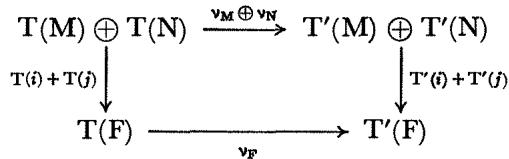
\includegraphics[keepaspectratio]{images/part002_2544dc0c.jpg}}

是可交换的，且竖直箭头是双射。

交换性由引理1得出，其余断言由§1第6号命题6的推论2以及§3第7号命题7得出。

引理3. 在引理2的假设下，\(\nu_{\mathrm{F}}\) 为单射（相应地，满射）的必要且充分条件是 \(\nu_{\mathrm{M}}\) 与 \(\nu_{\mathrm{N}}\) 皆然。

这由引理2及§1第6号命题6的推论1得出。

于是引理3连同§2第2号命题4表明，只需考虑F为自由模的情形。但若 \((b_{\mu})\) 是F的一组基，则 \(\operatorname{Hom}_{\mathbf{A}}(\mathbf{E}, \mathbf{G}) \otimes_{\mathbf{B}} \mathbf{F}\) 的每个元素都可唯一地写成 \(\sum_{\mu} u_{\mu} \otimes b_{\mu}\)，其中 \(u_{\mu} \in \operatorname{Hom}_{\mathbf{A}}(\mathbf{E}, \mathbf{G})\)（§3，第7号，命题7的推论1）；该元素在 \(\nu\) 下的像是 A-线性映射 \(x \mapsto \sum_{\mu} u_{\mu}(x) \otimes b_{\mu}\)；它不可能对所有 \(x \in \mathbf{E}\) 均为零，除非 \(u_{\mu}(x) = 0\)（对所有 \(x \in \mathbf{E}\) 与所有 \(\mu\) 成立），而这等价于 \(u_{\mu} = 0\)（对所有 \(\mu\)）；因此 \(\nu\) 是单射。当F还具有有限基时，引理3表明（通过对F的基中元素个数作归纳），要证明 \(\nu\) 是满射，只需就 \(F = B_s\) 的情形证明即可；但在此情形，(7) 式的两边都典范地等同于 \(\operatorname{Hom}_{\mathbf{A}}(\mathbf{E}, \mathbf{G})\)（§3，第4号，命题4），而 \(\nu\) 成为恒等映射。

\begin{enumerate}
\def\labelenumi{(\roman{enumi})}
\setcounter{enumi}{1}
\tightlist
\item
  为证明E为投射且有限生成时的命题，这次我们固定F与G，并对每个左A-模E记：
\end{enumerate}

\[
\mathrm{T} (\mathrm{E}) = \operatorname{Hom} _ {\mathrm{A}} (\mathrm{E}, \mathrm{G}) \otimes_ {\mathrm{B}} \mathrm{F}, \quad \mathrm{T} ^ {\prime} (\mathrm{E}) = \operatorname{Hom} _ {\mathrm{A}} (\mathrm{E}, \mathrm{G} \otimes_ {\mathrm{B}} \mathrm{F})
\]

并且，对于每一个左A模同态 \(v:\mathbf{E}\to\mathbf{E}^{\prime}\) ,

\[
\mathrm{T} (v) = \operatorname{Hom} (v, 1 _ {\mathbf {G}}) \otimes 1 _ {\mathbf {F}}, \quad \mathrm{T} ^ {\prime} (v) = \operatorname{Hom} (v, 1 _ {\mathbf {G}} \otimes 1 _ {\mathbf {F}});
\]

另一方面，我们用 \(\nu_{E}\) 代替 \(\nu\)。于是我们有以下两个引理：

引理4. 对于每个同态 \(v: \mathbf{E} \to \mathbf{E}'\) ，该图表

\[
\begin{array}{c c c} \mathrm{T} (\mathrm{E} ^ {\prime}) & \xrightarrow {\nu_ {\mathrm{E} ^ {\prime}}} & \mathrm{T} ^ {\prime} (\mathrm{E} ^ {\prime}) \\ \mathrm{T} (v) \Big \downarrow & & \Big \downarrow \mathrm{T} ^ {\prime} (v) \\ \mathrm{T} (\mathrm{E}) & \xrightarrow {\nu_ {\mathrm{E}}} & \mathrm{T} ^ {\prime} (\mathrm{E}) \end{array}\tag{10}
\]

是交换的。

引理5. 设 \(\mathbf{M}\) 与 \(\mathbf{N}\) 是 \(\mathbf{E}\) 中两个互补的子模，\(p: \mathbf{E} \to \mathbf{M}\)、\(q: \mathbf{E} \to \mathbf{N}\) 为典范投影。图表

\pandocbounded{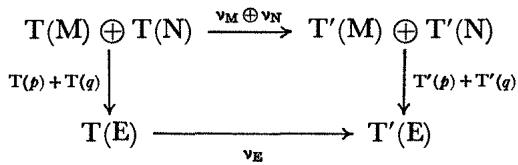
\includegraphics[keepaspectratio]{images/part002_a961576f.jpg}}

是可交换的，且竖直箭头是双射。

它们的证明与引理1和引理2相同，并用到§1第6号命题6的推论2、§2第1号命题1以及§3第7号命题7。

证明的余下部分随后按 (i) 的方式进行，并归结为 \(E = A_{s}\) 的情形；此时 (7) 式的两边典范地等同于 \(G \otimes_{B} F\)，而 \(\nu\) 成为恒等映射。

特别地，取 B = A 且 G 为 (A, A)-双模 \(_{s}A_{d}\)（§3，第4号），于是右A-模 \(\operatorname{Hom}_{\mathbf{A}}(\mathbf{E}, _{s}\mathbf{A}_{d})\) 就是E的对偶E*，并且 \((_{s}\mathbf{A}_{d}) \otimes_{\mathbf{A}} F\) 典范地等同于F（§3，第4号，命题4）。此时同态 (7) 成为典范Z-同态

\[
\theta : \mathrm{E} ^ {*} \otimes_ {\mathrm{A}} \mathrm{F} \rightarrow \operatorname{Hom} _ {\mathrm{A}} (\mathrm{E}, \mathrm{F})\tag{11}
\]

和 \(\theta (x^{*}\otimes y)\) 是E到F的线性映射

\[
x \mapsto \langle x, x ^ {*} \rangle y.
\]

注记（1）. §2 第6号命题12中给出的投射A模的刻画也可表述如下：对于左A模E为投射模，其充分必要条件为典范同态

\[
\theta_ {\mathbf {E}}: \mathrm{E} ^ {*} \otimes_ {\mathbf {A}} \mathrm{E} \rightarrow \operatorname{Hom} _ {\mathbf {A}} (\mathrm{E}, \mathrm{E}) = \operatorname{End} _ {\mathbf {A}} (\mathrm{E})
\]

使得 \(l_{E}\) 属于 \(\theta_{E}\) 的像。

推论. (i) 当F是投射（相应地，有限生成投射）模时，典范同态 (11) 是单射（相应地，双射）。

\begin{enumerate}
\def\labelenumi{(\roman{enumi})}
\setcounter{enumi}{1}
\tightlist
\item
  当E是有限生成投射模时，典范同态(11)是双射的。
\end{enumerate}

即使E与F都是有限生成的，\(\theta\) 也不一定满射，例 A = Z、E = F = Z/2Z 即说明这一点；(11) 式右端非零，但 \(E^{*} = 0\)。另一方面，可以给出E为自由模而 (11) 既非单射又非满射的例子（习题3(b)）。

当E具有有限基 \((e_i)\) 时，\(\theta^{-1}\)（\(\theta\) 的逆同构）可以如下显式求出。设 \((e_i^*)\) 为 \((e_i)\) 的对偶基（§2，第6号）；对所有 \(u \in \operatorname{Hom}(\mathbf{E}, \mathbf{F})\) 以及所有 \(x = \sum_{i} \xi_i e_i\)（其中 \(\xi_i \in \mathbf{A}\)），

\[
u (x) = \sum_ {i} \xi_ {i} u (e _ {i}) = \sum_ {i} \langle x, e _ {i} ^ {*} \rangle u (e _ {i})
\]

，从而 \(u = \sum_{i} \theta(e_i^* \otimes u(e_i))\)，换言之

\[
\theta^ {- 1} (u) = \sum_ {i} e _ {i} ^ {*} \otimes u (e _ {i}).\tag{12}
\]

特别地，若进一步有 F = E，则可看出 \(\theta_{E}^{-1}\) 把恒等映射 \(l_{E}\) 映为元素 \(\sum_{i} e_{i}^{*} \otimes e_{i}\)，因此该元素与E中所考虑的基 \((e_{i})\) 无关。

另一方面，注意当E是有限生成投射模时，\(\operatorname{End}_{\mathbf{A}}(\mathbf{E})\) 上的环结构可以通过 \(\theta_{E}^{-1}\) 转移到 \(E^{*}\otimes_{A}E\) 上；立即可以验证，对E中的 x, y 与 \(x^{*}, y^{*}\)（\(E^{*}\) 中的元素），在环 \(\operatorname{End}_{\mathbf{A}}(\mathbf{E})\) 中

\[
\theta_ {\mathbf {E}} (x ^ {*} \otimes x) \circ \theta_ {\mathbf {E}} (y ^ {*} \otimes y) = \theta_ {\mathbf {E}} ((y ^ {*} \langle y, x ^ {*} \rangle) \otimes x).\tag{13}
\]

注记 (2). 设 E 为右 A-模；在 (11) 中用 E* 替换 E，我们得到一个典范的 Z-同态

\[
\mathrm{E} ^ {* *} \otimes_ {\mathrm{A}} \mathrm{F} \rightarrow \operatorname{Hom} _ {\mathrm{A}} (\mathrm{E} ^ {*}, \mathrm{F}).\tag{14}
\]

另一方面，存在一个典范的 A-同态 \(c_{E}:E\to E^{**}\) ，由此得到一个 Z-同态 \(c_{E}\otimes l_{F}:E\otimes_{A}F\to E^{**}\otimes_{A}F\) ；将后者与同态 (14) 复合，我们从而得到一个典范的 Z-同态

\[
\theta^ {\prime}: \mathrm{E} \otimes_ {\mathrm{A}} \mathrm{F} \rightarrow \operatorname{Hom} _ {\mathrm{A}} (\mathrm{E} ^ {*}, \mathrm{F})\tag{15}
\]

使得 \(\theta'(x \otimes y)\) 是线性映射

\[
x ^ {*} \mapsto \langle x, x ^ {*} \rangle y.
\]

若 E 与 F 为投射模，则映射 (15) 是单射。因为 \(c_{E}\) 此时是单射（§2，第 7 号，命题 13 的推论 4），且由于 F 是投射的，Z-同态 \(c_{E} \otimes l_{F}: E \otimes_{A} F \to E^{**} \otimes_{A} F\) 也是单射（§3，第 7 号，命题 7 的推论 6）；最后，已见（命题 2）同态 (14) 是单射，由此得结论。

若 E 是投射且有限生成的，则映射 (15) 是双射，因为构成它的两个映射此时均为双射（§2，第 7 号，命题 13 的推论 4 及上文命题 2）。

\subsection{自同态的迹}

设 C 为交换环，E 为 C-模。映射 \((x^{*}, x) \mapsto \langle x, x^{*} \rangle\)（从 \(E^{*} \times E\) 到 C）是 C-双线性的，因为对所有 \(\gamma \in C\)，\(\langle \gamma x, x^{*} \rangle = \gamma \langle x, x^{*} \rangle\) 且 \(\langle x, x^{*} \gamma \rangle = \langle x, x^{*} \rangle \gamma\)；我们由此得到一个典范 C-线性映射

\[
\tau : \mathbf {E} ^ {*} \otimes_ {\mathbf {c}} \mathbf {E} \rightarrow \mathbf {C}\tag{16}
\]

使得 \(\tau(x^{*} \otimes x) = \langle x, x^{*} \rangle\)（§3，第5号）。现在再设E是有限生成的投射C-模；于是第2号的典范同构 (11) 是C-模同构，因此我们可以通过转移结构定义一个典范线性形式 \(\mathrm{Tr} = \tau \circ \theta_{\mathbf{E}}^{-1}\)（在C-模 \(\operatorname{End}_{\mathbf{C}}(\mathbf{E})\) 上）。对所有 \(u \in \operatorname{End}_{\mathbf{C}}(\mathbf{E})\)，标量 \(\operatorname{Tr}(u)\) 称为自同态 \(u\) 的迹；每个 \(u \in \operatorname{End}_{\mathbf{C}}(\mathbf{E})\) 都可以（一般以无穷多种方式）写成 \(x \mapsto \sum_{i} \langle x, x_{i}^{*} \rangle y_{i}\) 的形式，其中 \(x_{i}^{*} \in \mathbf{E}^{*}\)、\(y_{i} \in \mathbf{E}_{i}\)（依据第2号命题2的推论）；则

\[
\operatorname{Tr} (u) = \sum_ {i} \left\langle y _ {i}, x _ {i} ^ {*} \right\rangle \quad (\text { cf. } \S 1 0, \text { no. } 1 1).\tag{17}
\]

由定义，

\begin{enumerate}
\def\labelenumi{(\arabic{enumi})}
\setcounter{enumi}{17}
\tightlist
\item
\end{enumerate}

\[
\operatorname{Tr} (u + v) = \operatorname{Tr} (u) + \operatorname{Tr} (v)\tag{19}
\]

\[
\operatorname{Tr} (\gamma u) = \gamma \operatorname{Tr} (u)
\]

对 \(u, v\)（\(\operatorname{End}_{\mathbf{C}}(\mathbf{E})\) 中）及 \(\gamma \in \mathbf{C}\) 成立。此外：

命题3. 设 C 为交换环，E、F 为两个有限生成投射 C-模，且 \(u: \mathbf{E} \to \mathbf{F}\) 和 \(v: \mathbf{F} \to \mathbf{E}\) 为两个线性映射；则

\[
\operatorname{Tr} (v \circ u) = \operatorname{Tr} (u \circ v).\tag{20}
\]

映射 \((u, v) \mapsto \operatorname{Tr}(u \circ v)\) 与 \((u, v) \mapsto \operatorname{Tr}(v \circ u)\)（从

\[
\operatorname{Hom} _ {\mathbf {c}} (\mathbf {E}, \mathbf {F}) \times \operatorname{Hom} _ {\mathbf {c}} (\mathbf {F}, \mathbf {E})
\]

到C）都是 C-双线性的；因此只需在 u 形如 \(x \mapsto \langle x, a^{*} \rangle b\) 且 v 形如 \(y \mapsto \langle y, b^{*} \rangle a\)（其中 \(a \in E\)、\(a^{*} \in E^{*}\)、\(b \in F\)、\(b^{*} \in F^{*}\)）的情形验证 (20)。但此时 \(v \circ u\) 是映射 \(x \mapsto \langle x, a^{*} \rangle \langle b, b^{*} \rangle a\)，而 \(u \circ v\) 是映射 \(y \mapsto \langle y, b^{*} \rangle \langle a, a^{*} \rangle b\)。公式 (17) 表明 (20) 两端的值都等于 \(\langle a, a^{*} \rangle \langle b, b^{*} \rangle\)。

推论. 若 \(u_1, \ldots, u_p\) 是 \(\mathbf{E}\) 的自同态，则

\[
\operatorname{Tr} \left(u _ {1} \circ u _ {2} \circ \dots \circ u _ {p}\right) = \operatorname{Tr} \left(u _ {i} \circ u _ {i + 1} \circ \dots \circ u _ {p} \circ u _ {1} \circ \dots \circ u _ {i - 1}\right)
\]

对所有 \(1 \leqslant i \leqslant p\) 成立（“迹在循环置换下的不变性”）。

只需将 (20) 应用于乘积

\[
\left(u _ {1} \circ u _ {2} \circ \dots \circ u _ {i - 1}\right) \circ \left(u _ {i} \circ u _ {i + 1} \circ \dots \circ u _ {p}\right).
\]

注意另一方面，对于 E 的三个自同态 u、v、w，

\[
\operatorname{Tr} (u \circ v \circ w) = \operatorname{Tr} (u \circ w \circ v)
\]

不一定成立。

\subsection{\texorpdfstring{同态 \(\operatorname{Hom}_{\mathbb{C}}(\mathrm{E}_1, \mathrm{F}_1) \otimes_{\mathbb{C}} \operatorname{Hom}_{\mathbb{C}}(\mathrm{E}_2, \mathrm{F}_2) \to \operatorname{Hom}_{\mathbb{C}}(\mathrm{E}_1 \otimes_{\mathbb{C}} \mathrm{E}_2, \mathrm{F}_1 \otimes_{\mathbb{C}} \mathrm{F}_2)\)}{从 E1,F1 上的 Hom 与 E2,F2 上的 Hom 的 C 上张量积到相应张量积上的 Hom 的同态}}

设 C 为交换环，且 \(E_{1}\) , \(E_{2}\) , \(F_{1}\) , \(F_{2}\) 为四个 C-模；在 §3 第 5 号公式 (13) 中，我们定义了典范 C-模同态

\[
\lambda : \operatorname{Hom} (\mathbf {E} _ {1}, \mathbf {F} _ {1}) \otimes \operatorname{Hom} (\mathbf {E} _ {2}, \mathbf {F} _ {2}) \to \operatorname{Hom} (\mathbf {E} _ {1} \otimes \mathbf {E} _ {2}, \mathbf {F} _ {1} \otimes \mathbf {F} _ {2}). \tag {21}
\]

命题4. 当有序对 \((\mathbf{E}_1, \mathbf{E}_2)\)、\((\mathbf{E}_1, \mathbf{F}_1)\)、\((\mathbf{E}_2, \mathbf{F}_2)\) 之一由有限生成投射C-模组成时，典范同态 (21) 是双射。

显然，只需对有序对 \((\mathbf{E}_{1}, \mathbf{F}_{1})\) 与 \((\mathbf{E}_{1}, \mathbf{E}_{2})\) 证明即可。

我们先考虑有序对 \((\mathbf{E}_1, \mathbf{F}_1)\) 的情形；我们固定 \(\mathbf{E}_2, \mathbf{F}_1, \mathbf{F}_2\)，并对每个C-模记 \(\mathrm{T}(\mathbf{E}) = \mathrm{Hom}(\mathbf{E}, \mathbf{F}_1) \otimes_{\mathbb{C}} \mathrm{Hom}(\mathbf{E}_2, \mathbf{F}_2)\) 与 \(\mathrm{T}'(\mathbf{E}) = \mathrm{Hom}(\mathbf{E} \otimes \mathbf{E}_2, \mathbf{F}_1 \otimes \mathbf{F}_2)\)，且对每个C-同态 \(v: \mathbf{E} \to \mathbf{E}'\)，

\[
\mathrm{T} (v) = \operatorname{Hom} (v, \mathrm{l} _ {\mathrm{F} _ {1}}) \otimes \mathrm{l} _ {\operatorname{Hom} (\mathrm{E} _ {2}, \mathrm{F} _ {2})}
\]

和

\[
\mathrm{T} ^ {\prime} (v) = \operatorname{Hom} (v \otimes 1 _ {\mathbb {E} _ {2}}, 1 _ {\mathbf {F} _ {1} \otimes \mathbf {F} _ {2}}).
\]

于是引理4与引理5（第2号）（其中v换成了λ）成立，且可用完全类似的方法证明。

接下来我们固定 \(\mathbf{E}_2\) 与 \(\mathbf{F}_2\)，这次对每个C-模 \(\mathbf{F}\) 记 \(\mathrm{T}(\mathbf{F}) = \mathrm{Hom}(\mathbf{C},\mathbf{F})\otimes_{\mathbb{C}}\mathrm{Hom}(\mathbf{E}_2,\mathbf{F}_2)\) 与 \(\mathrm{T}'(\mathrm{F}) = \mathrm{Hom}(\mathbf{C}\otimes \mathbf{E}_2,\mathbf{F}\otimes \mathbf{F}_2)\)，且对每个C-同态 \(u:\mathrm{F}\to \mathrm{F}'\)，

\[
\mathrm{T} (u) = \operatorname{Hom} (\mathrm{l} _ {\mathbf {c}}, u) \otimes \mathrm{l} _ {\operatorname{Hom} (\mathbb {E} _ {2}, \mathrm{F} _ {2})}
\]

和

\[
\mathrm{T} ^ {\prime} (u) = \operatorname{Hom} (\mathrm{l} _ {\mathrm{c}} \otimes \mathrm{l} _ {\mathrm{E} _ {2}}, u \otimes \mathrm{l} _ {\mathrm{F} _ {2}}).
\]

这次可立即验证引理1与引理2（第2号）（其中 \(\lambda\) 处处代替 \(\nu\)）成立。

这样，我们先在 \(E_{1} = C\) 且 \(F_{1}\) 为投射且有限生成的情形证明该命题。第2号的论证（基于引理1与引理2）连同上述说明，把它归结为在 \(F_{1} = C\) 时证明该命题；于是 \(\operatorname{Hom}(E_{1}, F_{1})\)、\(E_{1} \otimes E_{2}\) 与 \(F_{1} \otimes F_{2}\) 分别等同于C、\(E_{2}\) 与 \(F_{2}\)（§3，第4号，命题4）；从而 (21) 式的两边都典范地等同于 \(\operatorname{Hom}(\mathbf{E}_{2},\mathbf{F}_{2})\)，且在这些等同之后，可验证 \(\lambda\) 成为恒等映射。

我们现在假设 \(F_{1}\) 是投射且有限生成的；第2号的论证（这次依赖引理4与引理5）把 \(E_{1}\) 为任意有限生成投射模时的证明归结为 \(E_{1} = C\) 的情形，即归结为已处理的第一种情形。

对于有序对 \((\mathbf{E}_{1}, \mathbf{E}_{2})\) ，过程类似，这次两次应用引理4和5；细节留给读者。

注意当 \(\mathbf{E}_1 = \mathbf{C}^{(I)}\)、\(\mathbf{E}_2 = \mathbf{C}^{(J)}\) 是自由模（不论是否有限生成）时，有 \(\operatorname{Hom}(\mathbf{E}_1, \mathbf{F}_1) = \mathbf{F}_1^{\mathrm{I}}\)、\(\operatorname{Hom}(\mathbf{E}_2, \mathbf{F}_2 = \mathbf{F}_2^{\mathrm{J}}\) 以及

\[
\operatorname{Hom} \left(\mathrm{E} _ {1} \otimes \mathrm{E} _ {2}, \mathrm{F} _ {1} \otimes \mathrm{F} _ {2}\right) = \left(\mathrm{F} _ {1} \otimes \mathrm{F} _ {2}\right) ^ {\mathrm{I} \times \mathrm{J}}
\]

（这在典范同构的意义下成立），且 (21) 此时就是§3第7号中典范同态 (22) 的一个特例。

当 \(E_{2} = C\) 时，把 \(\operatorname{Hom}(E_{2}, F_{2})\) 与 \(F_{2}\)、\(E_{1} \otimes E_{2}\) 与 \(E_{1}\) 等同后，典范同态 (21) 给出一个典范同态

\[
\operatorname{Hom} (\mathrm{E}, \mathrm{F}) \otimes \mathrm{G} \rightarrow \operatorname{Hom} (\mathrm{E}, \mathrm{F} \otimes \mathrm{G})\tag{22}
\]

对任意三个C-模E、F、G，它恰好是 \(\mathbf{A} = \mathbf{B} = \mathbf{C}\) 时第2号中的同态 (7)。

注意当 \(\mathbf{F} = \mathbf{C}\) 时，典范同态 (22) 再次给出交换环情形下的 (11)（第2号）。

现在假设 \(\mathbf{F}_1 = \mathbf{F}_2 = \mathbf{C}\)；由于 \(\mathbf{F}_1 \otimes \mathbf{F}_2\) 与 \(\mathbf{C}\) 等同，这次得到一个典范同态

\[
\mu : \mathbf {E} ^ {*} \otimes \mathbf {F} ^ {*} \rightarrow (\mathbf {E} \otimes \mathbf {F}) ^ {*}\tag{23}
\]

对于两个 C-模 E, F；对 \(x^{*} \in \mathbf{E}^{*}\)、\(y^{*} \in \mathbf{F}^{*}\)，\(x^{*} \otimes y^{*}\) 在典范同态 (23) 下的像是线性形式 \(u\)（\(\mathbf{E} \otimes \mathbf{F}\) 上的），满足

\[
u (x \otimes y) = \langle x, x ^ {*} \rangle \langle y, y ^ {*} \rangle .\tag{24}
\]

此外，若 \(E_{1}\) , \(E_{2}\) , \(F_{1}\) , \(F_{2}\) 是四个 C-模， \(f: E_{1} \rightarrow E_{2}\) , \(g: F_{1} \rightarrow F_{2}\) 是两个线性映射，则由 (24) 立即得出图表

\[
\begin{array}{c} \mathrm{E} _ {2} ^ {*} \otimes \mathrm{F} _ {2} ^ {*} \xrightarrow {\mu} (\mathrm{E} _ {2} \otimes \mathrm{F} _ {2}) ^ {*} \\ t _ {f} \otimes t _ {g} \Biggl \downarrow \qquad \qquad \qquad \qquad \qquad \qquad \qquad \qquad \qquad \qquad \qquad \qquad \qquad \qquad \qquad \qquad \qquad \qquad \qquad \qquad \qquad \qquad \qquad \qquad \qquad \qquad \qquad \qquad \qquad \qquad \qquad \qquad \qquad \qquad \\ \mathrm{E} _ {1} ^ {*} \otimes \mathrm{F} _ {1} ^ {*} \xrightarrow {\mu} (\mathrm{E} _ {1} \otimes \mathrm{F} _ {1}) ^ {*} \end{array}\tag{25}
\]

是交换的。

推论 1. 若模 E, F 中有一个是投射且有限生成的，则典范同态 (23) 是双射。

推论2. 设 \(\mathbf{E}_1, \mathbf{E}_2\) 是两个有限生成的投射C-模，\(u_1\) 是 \(\mathbf{E}_1\) 的一个自同态，\(u_2\) 是 \(\mathbf{E}_2\) 的一个自同态；则

\[
\operatorname{Tr} (u _ {1} \otimes u _ {2}) = \operatorname{Tr} (u _ {1}) \operatorname{Tr} (u _ {2}).\tag{26}
\]

由线性性，只需考虑 \(u_{1}\) 形如 \(x_{1} \mapsto \langle x_{1}, x_{1}^{*} \rangle y_{1}\) 且 \(u_{2}\) 形如 \(x_{2} \mapsto \langle x_{2}, x_{2}^{*} \rangle y_{2}\) 的情形；则 \(x_{1} \otimes x_{2}\) 在 \(u_{1} \otimes u_{2}\) 下的像按定义为

\[
\langle x _ {1}, x _ {1} ^ {*} \rangle \langle x _ {2}, x _ {2} ^ {*} \rangle (y _ {1} \otimes y _ {2}) = \langle x _ {1} \otimes x _ {2}, x _ {1} ^ {*} \otimes x _ {2} ^ {*} \rangle (y _ {1} \otimes y _ {2})
\]

其中 \(x_{1}^{*}\otimes x_{2}^{*}\) 在 \(\mu\) 下典范地等同于 \((\mathrm{E}_{1}\otimes\mathrm{E}_{2})^{*}\) 中的一个元素。由于 \(\langle y_{1}\otimes y_{2},x_{1}^{*}\otimes x_{2}^{*}\rangle=\langle y_{1},x_{1}^{*}\rangle\langle y_{2},x_{2}^{*}\rangle\)，公式 (26) 在此情形由 (17) 得出。

注记。若E、F、G是任意三个C-模，则容易验证图表

\[
\begin{array}{c} \mathrm{E} ^ {*} \otimes \mathrm{F} ^ {*} \otimes \mathrm{G} ^ {*} \xrightarrow {\mu \otimes 1} (\mathrm{E} \otimes \mathrm{F}) ^ {*} \otimes \mathrm{G} ^ {*} \\ 1 \otimes \mu \Biggl \downarrow \\ \mathrm{E} ^ {*} \otimes (\mathrm{F} \otimes \mathrm{G}) ^ {*} \xrightarrow [ \mu ]{} (\mathrm{E} \otimes \mathrm{F} \otimes \mathrm{G}) ^ {*} \end{array}\tag{27}
\]

是交换的，这可由公式(24)得出。

我们还注意到，在不假设C-模E、F有任何条件的情况下，存在典范同构

\begin{enumerate}
\def\labelenumi{(\arabic{enumi})}
\setcounter{enumi}{27}
\tightlist
\item
\end{enumerate}

\[
(\mathbf {E} \otimes \mathbf {F}) ^ {*} \rightarrow \operatorname{Hom} (\mathbf {E}, \mathbf {F} ^ {*})\tag{29}
\]

\[
(\mathbf {E} \otimes \mathbf {F}) ^ {*} \rightarrow \operatorname{Hom} (\mathbf {F}, \mathbf {E} ^ {*})
\]

它们即第1号中取 \(\mathbf{G} = \mathbf{C}\)、\(\mathbf{A} = \mathbf{B} = \mathbf{C}\) 时的同构 (6) 与 (5)。

这样，在 \(E \times F\) 上的双线性形式、从E到 \(F^{*}\) 的同态与从F到 \(E^{*}\) 的同态之间，就定义了一个典范的一一对应：若 u（相应地 v）是从E到 \(F^{*}\)（相应地，从F到 \(E^{*}\)）的同态，则相应的双线性形式由下式给出

\[
(x, y) \mapsto \langle y, u (x) \rangle \quad (\text { resp. } (x, y) \mapsto \langle x, v (y) \rangle).
\]

\section{标量环的扩张}

\subsection{模的标量环的扩张}

设 A、B 为两个环，\(\rho: \mathbf{A} \to \mathbf{B}\) 为环同态；我们考虑由该同态定义的右A-模 \(\rho^{*}(B_{d})\)（§1，第13号）；这个A-模还具有左B-模结构，即 \(B_{s}\) 的结构，并且由于 \(b'(b\rho(a)) = (b'b)\rho(a)\)（对 \(a \in \mathbf{A}\) 及B中的 \(b\)、\(b'\)），B上的这两个模结构是相容的（§1，第14号）。这使我们可以对每个左A-模E，在张量积 \(\rho_{*}(B_{d}) \otimes_{\mathbf{A}} \mathbf{E}\) 上定义一个左B-模结构，使得 \(\beta'(\beta \otimes x) = (\beta'\beta) \otimes x\)（对B中的 \(\beta\)、\(\beta'\) 及 \(x \in \mathbf{E}\)）（§3，第3号）。这个左B-模称为借助 \(\rho\) 把标量环扩张到B而由E导出的模，记作 \(\rho^{*}(\mathbf{E})\) 或 \(\mathrm{E}_{(\mathbf{B})}\)（不致混淆时）。

对每个左A-模E，映射 \(\phi: x \mapsto 1 \otimes x\)（从E到A-模 \(\rho_*(\rho^*(\mathbf{E}))\)）是A-线性的，且集合 \(\phi(\mathbf{E})\) 生成B-模 \(\rho^*(\mathbf{E})\)。进而，对每个左B-模F与每个A-线性映射 \(f\)（从E到A-模 \(\rho_*(\mathbf{F})\)），存在唯一的B-线性映射 \(\tilde{f}\)（从 \(\rho^*(\mathbf{E})\) 到F），使得 \(\tilde{f}(1 \otimes x) = f(x)\)（对所有 \(x \in \mathbf{E}\)）。

B 可借助 \(\rho\) 视为一个 (B, A)-双模；于是存在一个典范的 Z-模同构

\[
\operatorname{Hom} _ {\mathbf {B}} (\mathbf {B} \otimes_ {\mathbf {A}} \mathbf {E}, \mathbf {F}) \rightarrow \operatorname{Hom} _ {\mathbf {A}} (\mathbf {E}, \operatorname{Hom} _ {\mathbf {B}} (\mathbf {B} _ {s}, \mathbf {F}))\tag{1}
\]

这正如§4第1号命题1所示。但左A-模 \(\mathrm{Hom}_{\mathbf{B}}(\mathbf{B}_{s},\mathbf{F})\) 典范地等同于 \(\rho^{*}(\mathbf{F})\)：因为按定义（§1，第14号），对元素 \(y\in \mathbf{F}\) 对应着同态 \(\theta (y)\colon \mathbf{B}_s\to \mathbf{F}\)，它满足 \((\theta (y))(1) = y\)；于是对所有 \(\lambda \in \mathbf{A}\)，对 \(\rho (\lambda)y\in \mathbf{F}\) 对应着同态 \(\mu \mapsto \mu \rho (\lambda)y\)（从 \(\mathbf{B}_s\) 到 \(\mathbf{F}\) 的），它正是 \(\lambda \theta (y)\)（对 \(\mathrm{Hom}_{\mathbf{B}}(\mathbf{B}_{s},\mathbf{F})\) 的左A-模结构而言）（§1，第14号）。利用这一等同，我们因此得到一个典范Z-模同构，即 (1) 的逆

\[
\delta : \operatorname{Hom} _ {\mathbf {A}} (\mathbf {E}, \rho_ {*} (\mathbf {F})) \rightarrow \operatorname{Hom} _ {\mathbf {B}} (\rho^ {*} (\mathbf {E}), \mathbf {F})\tag{2}
\]

并且由定义立即得出，若 \(\delta(f) = \bar{f}\)，则 \(\bar{f}(1 \otimes x) = f(x)\)（对所有 \(x \in \mathbf{E}\)）。特别地，映射 \(\phi_{\mathbb{E}}: x \mapsto 1 \otimes x\) 恰好就是

\[
\phi_ {\mathbf {E}} = \delta^ {- 1} (1 _ {\rho^ {*} (\mathbf {E})}).\tag{3}
\]

因此，命题1得证。该映射 \(\phi_{\mathbf{E}}: \mathbf{E} \to \rho_{*}(\rho^{*}(\mathbf{E}))\) 被称为典范的。

注. (1) 命题1表明，由 \(\mathbf{E}_{(\mathbf{B})}\) 与 \(\phi_{\mathbb{E}}\) 组成的有序对是泛映射问题（集合论，IV，§3，第1号）的一个解，其中 \(\Sigma\) 是左B-模结构的物种（态射为B-线性映射），而 \(\alpha\)-映射是E到某个B-模中的A-线性映射。

\begin{enumerate}
\def\labelenumi{(\arabic{enumi})}
\setcounter{enumi}{1}
\item
  若E是一个 \((\mathbf{A}, (\mathbf{C}_{i}^{\prime}); (\mathbf{D}_{j}^{\prime}))\) -多模且F是一个 \((\mathbf{B}, (\mathbf{C}_{h}^{\prime\prime}); (\mathbf{D}_{k}^{\prime\prime}))\) -多模，则同构(2)关于两边的 \(((\mathbf{D}_{j}^{\prime}), (\mathbf{C}_{h}^{\prime\prime}); (\mathbf{C}_{i}^{\prime}), (\mathbf{D}_{k}^{\prime\prime}))\) -多模结构是线性的（§1，第14号及§3，第4号）。
\item
  设E为左A-模，a为A的双边理想，且 \(\rho:A\to A/a\) 为典范同态。在§3第6号命题6推论2的记号下，A-模E/aE被a零化，因此典范地具有左(A/a)-模结构（§1，第12号）；显然，§3第6号命题6推论2中定义的典范映射 \(\pi:\rho^{*}(E)\to E/aE\) 对于(A/a)-模结构是同构。
\end{enumerate}

推论。设E，E'为两个左A-模；对每个A-线性映射u: E → E'，v = l\_B ⊗ u是使下图交换的唯一B-线性映射

\pandocbounded{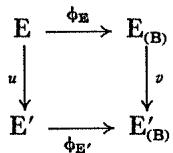
\includegraphics[keepaspectratio]{images/part002_74d11806.jpg}}

（其中 \(\phi_{\mathbf{E}}\) 与 \(\phi_{\mathbf{E}'}\) 是典范映射）。

只需将命题1应用于A-同态 \(\phi_{\mathbf{E}'} \circ u: \mathbf{E} \to \mathbf{E}_{(\mathbf{B})}'\)。

上述推论中定义的映射 \(v\) 记作 \(\rho^{*}(u)\) 或 \(u_{(B)}\)。若 \(E''\) 是第三个左A-模且 \(v: E' \to E''\) 为A-线性映射，则显然

\[
\left(v \circ u\right) _ {(\mathbf {B})} = v _ {(\mathbf {B})} \circ u _ {(\mathbf {B})}.
\]

模的算子环的扩张是一种可传递的运算；确切地说：

命题2. 设 \(\rho: \mathbf{A} \to \mathbf{B}\) , \(\sigma: \mathbf{B} \to \mathbf{C}\) 是环同态。对每个左A-模E，存在唯一的C-同态

\[
\sigma^ {*} (\rho^ {*} (\mathrm{E})) \rightarrow (\sigma \circ \rho) ^ {*} (\mathrm{E})\tag{4}
\]

它把 \(1 \otimes (1 \otimes x)\) 映为 \(1 \otimes x\)（对所有 \(x \in E\)），且该同态是双射。

\(\sigma^{*}(\rho^{*}(\mathbf{E}))\) 与 \((\sigma \circ \rho)^{*}(\mathbf{E})\) 的底层Z-模分别是 \(\mathbf{C} \otimes_{\mathbf{B}} (\mathbf{B} \otimes_{\mathbf{A}} \mathbf{E})\) 与 \(\mathbf{C} \otimes_{\mathbf{A}} \mathbf{E}\)。存在一个典范Z-同构 \(\mathbf{C} \otimes_{\mathbf{B}} (\mathbf{B} \otimes_{\mathbf{A}} \mathbf{E}) \to (\mathbf{C} \otimes_{\mathbf{B}} \mathbf{B}) \otimes_{\mathbf{A}} \mathbf{E}\) （§ 3，第8号，命题8），它对于两侧的左C-模结构也是C-同构。此外，C-模C ⊗B B在映射γ ⊗ β到γσ(β)的同构下典范地等同于C-模Cs（§ 3，第4号，命题4），并且该同构也是对于由ρ定义的C ⊗B B上的右A-模结构和由σ ∘ ρ定义的C上的右A-模结构的同构。因此，存在一个典范同构

\[
(\mathbf {C} \otimes_ {\mathbf {B}} \mathbf {B}) \otimes_ {\mathbf {A}} \mathbf {E} \rightarrow \mathbf {C} \otimes_ {\mathbf {A}} \mathbf {E}
\]

于是就得到；将它与同构

\[
\mathbf {C} \otimes_ {\mathbf {B}} (\mathbf {B} \otimes_ {\mathbf {A}} \mathbf {E}) \rightarrow (\mathbf {C} \otimes_ {\mathbf {B}} \mathbf {B}) \otimes_ {\mathbf {A}} \mathbf {E}
\]

复合，就得到所需的典范同构。

若 \(\phi, \phi'\) 和 \(\phi''\) 分别记典范映射 \(E \to \rho^*(E)\) , \(\rho^*(E \to) \sigma^*(\rho^*(E))\) 和 \(E \to (\sigma \circ \rho)^*(E)\) ,则在命题2的典范同构下，\(\phi' \circ \phi\) 与 \(\phi''\) 等同。

命题3. 设A，B为两个交换环， \(\rho: \mathbf{A} \to \mathbf{B}\) 为环同态，且 E、E' 是两个 A-模。存在唯一的 B-同态

\[
\mathbf {E} _ {(\mathbf {B})} \otimes_ {\mathbf {B}} \mathbf {E} _ {(\mathbf {B})} ^ {\prime} \rightarrow (\mathbf {E} \otimes_ {\mathbf {A}} \mathbf {E} ^ {\prime}) _ {(\mathbf {B})}\tag{5}
\]

它把 \((1 \otimes x) \otimes (1 \otimes x')\) 映为 \(1 \otimes (x \otimes x')\)（对 \(x \in \mathbf{E}\)、\(x' \in \mathbf{E}'\)），且该同态是双射。

（5）的左边可写成 \((\mathbf{B} \otimes_{\mathbf{A}} \mathbf{E}) \otimes_{\mathbf{B}} (\mathbf{B} \otimes_{\mathbf{A}} \mathbf{E}')\)，且（因A与B交换）与 \((\mathbf{E} \otimes_{\mathbf{A}} \mathbf{B}) \otimes_{\mathbf{B}} (\mathbf{B} \otimes_{\mathbf{A}} \mathbf{E}')\) 等同；后一个乘积依次等同于 \(\mathbf{E} \otimes_{\mathbf{A}} (\mathbf{B} \otimes_{\mathbf{B}} \mathbf{B}) \otimes_{\mathbf{A}} \mathbf{E}'\) , \(\mathbf{E} \otimes_{\mathbf{A}} (\mathbf{B} \otimes_{\mathbf{A}} \mathbf{E}')\) , \(\mathbf{E} \otimes_{\mathbf{A}} (\mathbf{E}' \otimes_{\mathbf{A}} \mathbf{B})\) ，最终等同于 \((\mathbf{E} \otimes_{\mathbf{A}} \mathbf{E}') \otimes_{\mathbf{A}} \mathbf{B}\) ，这利用了张量积的结合性（§3，第8号，命题8）、§3第4号命题4以及A与B的交换性。所需的同构是这些相继的典范同构的复合。

显然，若S是E的一个生成系，则S在典范映射 \(E \rightarrow E_{(B)}\) 下的像是 \(E_{(B)}\) 的一个生成系；特别地，若E是有限生成的A-模，则 \(E_{(B)}\) 是有限生成的B-模。

命题4. 设E是具有基 \((a_{\lambda})_{\lambda \in L}\) 的A-模；若 \(\phi : x \mapsto 1 \otimes x\) 是E到 \(\rho^{*}(\mathbf{E})\) 的典范映射，则 \((\phi(a_{\lambda}))_{\lambda \in L}\) 是 \(\rho^{*}(\mathbf{E})\) 的一组基。若 \(\rho\) 是单射，则 \(\phi\) 亦然。

第一个断言直接由§3第7号命题7的推论1得出。此外，对A中元素的每个有限支撑族 \((\xi_{\lambda})_{\lambda \in L}\)，有 \(\phi\left(\sum_{\lambda \in L} \xi_{\lambda} a_{\lambda}\right) = \sum_{\lambda \in L} \rho(\xi_{\lambda}) \phi(a_{\lambda})\)，因而关系 \(\phi\left(\sum_{\lambda \in L} \xi_{\lambda} a_{\lambda}\right) = 0\) 等价于 \(\rho(\xi_{\lambda}) = 0\)（对所有 \(\lambda \in L\)），由此得出第二个断言。

推论. 对每个投射A-模E，B-模 \(\rho^{*}(\mathbf{E})\) 是投射的。若进一步 \(\rho\) 是单射，则E到 \(\rho^{*}(\mathbf{E})\) 的典范映射是单射。

由假设，存在一个包含E的自由A-模M，且E在M中有一个补子模F。由§3第7号命题7直接可得，\(\mathbf{M}_{(\mathbf{B})}\) 等同于 \(\mathbf{E}_{(\mathbf{B})}\) 与 \(\mathbf{F}_{(\mathbf{B})}\) 的直和，且若 \(\phi\) 和 \(\psi\) 是典范映射 \(\mathbf{E} \to \mathbf{E}_{(\mathbf{B})}\) 和 \(\mathbf{F} \to \mathbf{F}_{(\mathbf{B})}\)，则典范映射 \(\mathbf{M} \to \mathbf{M}_{(\mathbf{B})}\) 就是 \(x + y \mapsto \phi(x) + \psi(y)\)。该推论由命题4应用于A-模M直接得出。

当E是右A-模时，我们类似地记 \(\rho^{*}(\mathbf{E}) = \mathbf{E} \otimes_{\mathbf{A}} \rho_{*}(\mathbf{B}_{s})\)，此时将 B 视为 (A, B)-双模，且 \(\rho^{*}(\mathbf{E})\) 上的右B-模结构满足 \((x \otimes \beta)\beta' = x \otimes (\beta\beta')\)（对 \(\beta \in B, \beta' \in B\) 和 \(x \in E\)）。我们把本小节及下一小节中相应于右模的结果的陈述留给读者自行完成。

注记（4）. 考虑左A-模 \(\rho_{*}(B_{s})\)（由 \(\rho\) 定义），并且对每个左A-模E，考虑Z-模

\[
\tilde {\rho} (\mathbf {E}) = \operatorname{Hom} _ {\mathbf {A}} \left(\rho_ {*} \left(\mathbf {B} _ {s}\right), \mathbf {E}\right).\tag{6}
\]

由于 \(\rho_{*}(\mathbf{B}_{s})\) 具有右B-模结构，在 \(\tilde{\rho}(\mathbf{E})\) 上导出一个左B-模结构（\(\S 1\)，第14号），使得若 \(u \in \tilde{\rho}(\mathbf{E})\) 且 \(b' \in \mathbf{B}\)，则 \(b'u\) 是同态 \(b \mapsto u(bb')\)（从 \(\rho_{*}(\mathbf{B}_{s})\) 到 \(\mathbf{E}\)）。我们进一步定义一个称为典范的A-线性映射

\[
\eta : \rho_ {*} (\tilde {\rho} (\mathbf {E})) \rightarrow \mathbf {E}\tag{7}
\]

它把每个同态 \(u \in \tilde{\rho}(\mathbf{E})\) 对应到元素 \(u(1)\)（在 \(\mathbf{E}\) 中）。由于 \(\mathbf{B}\) 可借助 \(\rho\) 被视为一个(A, B)-双模，对每个左B-模 \(\mathbf{F}\)，存在一个典范的 \(\mathbf{Z}\)-模同构

\[
\operatorname{Hom} _ {\mathbf {A}} \left(\rho_ {*} (\mathrm{B} _ {s}) \otimes_ {\mathrm{B}} \mathrm{F}, \mathrm{E}\right)\rightarrow \operatorname{Hom} _ {\mathbf {B}} (\mathrm{F}, \operatorname{Hom} _ {\mathbf {A}} \left(\rho_ {*} (\mathrm{B} _ {s}), \mathrm{E}\right))
\]

（§1，第1号，命题1）。由于左A-模 \(\rho^{*}(B_{s}) \otimes_{B} F\) 依据§3第4号命题4典范地等同于 \(\rho_{*}(F)\)，我们得到一个典范Z-模同构，即上述同构的逆

\[
\operatorname{Hom} _ {\mathbf {B}} (\mathbf {F}, \tilde {\rho} (\mathbf {E})) \rightarrow \operatorname{Hom} _ {\mathbf {A}} (\rho_ {*} (\mathbf {F}), \mathbf {E})\tag{8}
\]

它把每个从F到 \(\tilde{\rho}(\mathbf{E})\) 的B-线性映射g对应到复合映射 \(\eta \circ g\)，视为从 \(\rho_{*}(\mathbf{F})\) 到E的A-线性映射。特别地，在命题2的假设下，若把F换成 \(\sigma_{*}(\mathbf{C}_{s})\)，则得到典范C-同构

\[
\tilde {\sigma} (\tilde {\rho} (\mathbf {E})) \rightarrow (\sigma \circ \rho) ^ {\sim} (\mathbf {E}).\tag{9}
\]

\subsection{标量环的限制与扩张之间的关系}

设 \(\rho: \mathbf{A} \to \mathbf{B}\) 为环同态。对每个左A-模E，典范A-线性映射

\[
\phi_ {\mathbf {E}}: \mathbf {E} \rightarrow \rho_ {*} (\rho^ {*} (\mathbf {E}))\tag{10}
\]

已在第1号中定义，使得 \(\phi_{\mathbb{E}}(x) = 1 \otimes x\)。现在我们考虑左B-模F，并将命题1（第1号）应用于A-同态 \(\mathbf{l}_{\rho_{*}(\mathbf{F})}: \rho_{*}(\mathbf{F}) \to \rho_{*}(\mathbf{F})\)：我们得到一个B-线性映射

\[
\psi_ {\mathbf {F}} \colon \rho^ {*} (\rho_ {*} (\mathbf {F})) \rightarrow \mathbf {F}\tag{11}
\]

等于 \(\delta(1_{\rho_*(\mathbb{F})})\) 并且因此使得，对所有 \(y \in \mathbb{F}\) 以及所有 \(\beta \in \mathbb{B}\) , \(\psi_{\mathbb{F}}(\beta \otimes y) = \beta y\) .

命题5. 设E为左A-模，F为左B-模；复合映射

\[
\rho^ {*} (\mathrm{E}) \xrightarrow [ \rho^ {*} (\phi_ {\mathrm{E}}) ]{} \rho^ {*} (\rho_ {*} (\rho^ {*} (\mathrm{E}))) \xrightarrow [ \psi_ {\rho^ {*} (\mathrm{E})} ]{} \rho^ {*} (\mathrm{E})\tag{12}
\]

\[
\rho_ {*} (\mathrm{F}) \xrightarrow [ \phi_ {\rho_ {*} (\mathrm{F})} ]{} \rho_ {*} (\rho^ {*} (\rho_ {*} (\mathrm{F}))) \xrightarrow [ \rho_ {*} (\psi_ {\mathrm{F}}) ]{} \rho_ {*} (\mathrm{F})\tag{13}
\]

分别等于 \(\rho^{*}(\mathbf{E})\) 与 \(\rho_{*}(\mathbf{F})\) 的恒等映射。

我们给出(12)的证明作为例子；对所有 \(x \in \mathbf{E}\)，映射 \(\rho^{*}(\phi_{\mathbf{E}})\) 把 \(1 \otimes x\) 映为元素 \(1 \otimes (1 \otimes x)\)，且映射 \(\psi_{\rho^{*}(\mathbf{E})}\) 把 \(1 \otimes (1 \otimes x)\) 映为元素 \(1 \otimes x\)；结论由形如 \(1 \otimes x\) 的元素生成B-模 \(\rho^{*}(\mathbf{E})\) 这一事实得出；(13)的证明甚至更简单。

推论. 映射 \(\rho^{*}(\phi_{\mathbf{E}})\) 和 \(\phi_{\rho^{*}(\mathbf{F})}\) 是单射，并且分别把 \(\rho^{*}(\mathbf{E})\) 等同于 \(\rho^{*}(\rho_{*}(\rho^{*}(\mathbf{E})))\) 的一个直因子，把 \(\rho_{*}(\mathbf{F})\) 等同于 \(\rho_{*}(\rho^{*}(\rho_{*}(\mathbf{F})))\) 的一个直因子。

这是命题5及§1第9号中命题15的推论2的直接结果。

命题6. 设E为左A-模，F为右B-模。则存在唯一的Z-同态

\[
\rho_ {*} (\mathrm{F}) \otimes_ {\mathrm{A}} \mathrm{E} \rightarrow \mathrm{F} \otimes_ {\mathrm{B}} \rho^ {*} (\mathrm{E})\tag{14}
\]

它把 \(y \otimes x\) 映为 \(y \otimes (1 \otimes x)\)（对所有 \(x \in E\) 及所有 \(y \in F\)），且该同态是双射。

根据定义，（14）的右边是 \(F \otimes_{B} (B \otimes_{A} E)\)，其中B被视为(B, A)-双模，并且存在一个§3第8号命题8中定义的典范Z-同构 \((\mathbf{F} \otimes_{\mathbf{B}} \mathbf{B}) \otimes_{\mathbf{A}} \mathbf{E} \to \mathbf{F} \otimes_{\mathbf{B}} (\mathbf{B} \otimes_{\mathbf{A}} \mathbf{E})\)；另一方面，§3第4号命题4中的典范同构 \(F \to F \otimes_{B} B\) 对由 \(\rho\) 定义的两侧右A-模结构是同构。由此得到所期望的同构。

当A与B交换时，同构(14)是A-模同构

\[
\rho_ {*} (\mathrm{F}) \otimes_ {\mathrm{A}} \mathrm{E} \rightarrow \rho_ {*} (\mathrm{F} \otimes_ {\mathrm{B}} \rho^ {*} (\mathrm{E})).
\]

\subsection{同态模的算子环的扩张}

设A为交换环，B为环， \(\rho: \mathbf{A} \to \mathbf{B}\) 为环同态，E、F为两个A-模；由于B（借助 \(\rho\)）是(A,A)-双模，且F可视为(A,A)-双模，因此在Z-模 B \(\otimes_{\mathbf{A}}\) F 上有两种A-模结构，在这些结构下分别有 \(a(b \otimes y) = (\rho(a)b) \otimes y\) 和 \(a(b \otimes y) = b \otimes (ay)\)（对 \(a \in \mathbf{A}\)、\(b \in \mathbf{B}\)、\(y \in \mathbf{F}\)）。我们把这样定义的两个A-模记为G'和G''；此外，G'恰好就是A-模 \(\rho_*(\rho^*(\mathbf{F}))\)。

这样一来，在§4第2号公式(7)的典范同态的定义中，我们把B换成A，把B-模F换成借助 \(\rho\) 视为A-模的环B，并把G换成视为(A, A)-双模的F；由于A交换，所得的典范Z-同态可写作

\[
\mathbf {B} \otimes_ {\mathbf {A}} \operatorname{Hom} _ {\mathbf {A}} (\mathbf {E}, \mathbf {F}) \rightarrow \operatorname{Hom} _ {\mathbf {A}} (\mathbf {E}, \mathbf {G} ^ {\prime \prime}).\tag{15}
\]

另一方面（第1号，公式(2)），存在一个典范Z-同构

\[
\mathrm{Hom} _ {\mathbf {A}} (\mathbf {E}, \mathbf {G} ^ {\prime}) = \mathrm{Hom} _ {\mathbf {A}} (\mathbf {E}, \rho_ {*} (\rho^ {*} (\mathbf {F}))) \rightarrow \mathrm{Hom} _ {\mathbf {B}} (\rho^ {*} (\mathbf {E}), \rho^ {*} (\mathbf {F})). \tag {16}
\]

现在假设 \(\rho(A)\) 包含于 \(B\) 的中心，这时 \(\rho\) 也称为中心同态 \(*\)（或称 \(\rho\) 在 \(B\) 上定义了一个A-代数结构，参见III，§1，第3号）。则 \(G'\) 与 \(G''\) 的A-模结构相同，并且把同态（16）与（15）复合，我们从而得到一个典范Z-同态

\[
\omega : \mathrm{B} \otimes_ {\mathrm{A}} \operatorname{Hom} _ {\mathrm{A}} (\mathrm{E}, \mathrm{F}) \rightarrow \operatorname{Hom} _ {\mathrm{B}} \left(\mathrm{E} _ {(\mathrm{B})}, \mathrm{F} _ {(\mathrm{B})}\right)\tag{17}
\]

其特征是，对于所有 \(u \in \operatorname{Hom}_{\mathbf{A}}(\mathbf{E}, \mathbf{F})\) 以及所有 \(b \in B\)

\[
\omega (b \otimes u) = r _ {b} \otimes u,\tag{18}
\]

其中 \(r_b\) 表示B中右乘 \(b\) 的映射。

此外，\(\omega\) 是中心同态这一假设蕴含 \((bb')\rho(a) = b\rho(a)b'\)（对B中的 \(b, b'\) 及 \(a \in A\)）；换言之，\(B_d\) 的右B-模结构与其A-模结构相容；从而它在 B \(\otimes_A\) \(\mathrm{Hom}_{\mathbf{A}}(\mathbf{E}, \mathbf{F})\) 上定义了一个右B-模结构（§3，第4号），也在 \(\mathrm{F}_{(\mathbf{B})} = \mathbf{B} \otimes_{\mathbf{A}} \mathbf{F}\) 上定义一个；最后，由于 \(\mathrm{F}_{(\mathbf{B})}\) 上的左、右B-模结构相容，在 \(\mathrm{Hom}_{\mathbf{B}}(\mathrm{E}_{(\mathbf{B})}, \mathrm{F}_{(\mathbf{B})})\) 上也得到一个右B-模结构（§1，第14号）。然后立即验证（17）对这些结构是右B-模同态。

命题7. 设 A 是一个交换环，B 是一个环， \(\rho: \mathbf{A} \to \mathbf{B}\) 一个中心同态，且 E、F 是两个 A-模。

\begin{enumerate}
\def\labelenumi{(\roman{enumi})}
\item
  若 B 是投射（相应地，有限生成投射）A-模，则同态 (17) 是单射（相应地，双射）。
\item
  若 \(\mathbf{E}\) 是有限生成的投射A-模，则同态 (17) 是双射。
\end{enumerate}

由于（16）是双射，该命题由§4第2号命题2应用于典范同态（15）得出。

\subsection{通过标量扩张得到的模的对偶}

设 A、B 为两个环， \(\rho: \mathbf{A} \to \mathbf{B}\) 一个环同态，E 是一个左 A-模，且 \(\mathbf{E}^*\) 其对偶。我们将定义一个典范的B-线性映射。

\[
\nu _ {E}: (E ^ {*}) _ {(B)} \rightarrow (E _ {(B)}) ^ {*}.\tag{19}
\]

(19) 的左边可写成 \(\mathrm{Hom}_{\mathbf{A}}(\mathbf{E},\mathbf{A})\otimes_{\mathbf{A}}\rho_{*}(\mathbf{B}_{s})\)，其中在 \(\mathrm{Hom}_{\mathbf{A}}(\mathbf{E},\mathbf{A})\) 中，\(\mathbf{A}\) 被视为 \((\mathbf{A},\mathbf{A})\)-双模。则存在一个典范 \(\mathbf{Z}\)-同态（\(\S 4\)，第2号，公式(7)）

\[
\nu: \operatorname{Hom} _ {A} (E, A) \otimes_ {A} \rho_ {*} (B _ {s}) \rightarrow \operatorname{Hom} _ {A} (E, A \otimes_ {A} \rho_ {*} (B _ {s})) = \operatorname{Hom} _ {A} (E, \rho_ {*} (B _ {s}))
\]

利用§3第4号命题4中的典范同构给出的等同关系。另一方面，(19)式的右端可以写成 \(\mathrm{Hom}_{\mathbf{B}}(\rho_{*}(\mathbf{B}_{d}) \otimes_{\mathbf{A}} \mathbf{E}, \mathbf{B}_{s})\) ；由于B是(B, A)-双模，存在一个典范的Z-同构（§4第1号命题1）

\[
\beta : \operatorname{Hom} _ {\mathbf {B}} (\rho_ {*} (\mathbf {B} _ {d}) \otimes_ {\mathbf {A}} \mathbf {E}, \mathbf {B} _ {s}) \rightarrow \operatorname{Hom} _ {\mathbf {A}} (\mathbf {E}, \operatorname{Hom} _ {\mathbf {B}} (\mathbf {B} _ {s}, \mathbf {B} _ {s}))
\]

和 \(\mathrm{Hom}_{\mathbb{B}}(\mathbf{B}_s,\mathbf{B}_s)\) 作为 A-模，典范地等同于 \(\rho_{*}(\mathbf{B}_{s})\) （参见第 1 号，命题 1 的证明）。考虑到这些等同，我们得到同态 \(\nu_{\mathbb{E}}\) ；容易验证该同态由等式

\[
\langle \xi \otimes x, \nu _ {E} (x ^ {*} \otimes \eta) \rangle = \xi_ {\rho} (\langle x, x ^ {*} \rangle) \eta ,\tag{20}
\]

（对 \(x \in \mathbf{E}\)、\(x^{*} \in \mathbf{E}^{*}\)、\(\xi\)、\(\eta\) 属于 \(\mathbf{B}\)）所刻画，这立即表明 \(\nu_{\mathbf{E}}\) 是B-线性的。此外，对每个A-线性映射 \(u: \mathbf{E} \to \mathbf{F}\)，图表

\[
\begin{array}{c c c} (\mathrm{F} ^ {*}) _ {(\mathrm{B})} & \xrightarrow {\nu_ {\mathrm{F}}} & (\mathrm{F} _ {(\mathrm{B})}) ^ {*} \\ \Big \downarrow^ {(t _ {u}) _ {(\mathrm{B})}} & & \Big \downarrow^ {t (u _ {(\mathrm{B})})} \\ (\mathrm{E} ^ {*}) _ {(\mathrm{B})} & \xrightarrow {\nu_ {\mathrm{E}}} & (\mathrm{E} _ {(\mathrm{B})}) ^ {*} \end{array}
\]

是交换的。

命题8. 若A-模E与 \(\rho_{*}(B_{s})\) 之一是投射且有限生成的，则同态 \(\nu_{\mathbb{E}}\) 是双射。

这由上述内容及第4节第2号命题2得出。

特别地，假设E是有限生成的自由A-模，令 \((e_{i})_{1\leqslant i\leqslant n}\) 为E的一组基，\((e_{i}^{*})\) 为其对偶基；则典范同构（19）把基 \((e_{i}^{*}\otimes1)\)（属于 \((\mathrm{E}^{*})_{(\mathrm{B})}\)）映为 \((1\otimes e_{i})\)（\(\mathrm{E}_{(\mathrm{B})}\) 的基）的对偶基。

\subsection{有限性判据}

命题9. 设 B 是一个环，A 是 B 的一个子环，且 P 是一个投射左 A-模。那么，如果 \(P_{(B)}\) 是有限生成的 B-模，则 P 本身是有限生成的 A-模。

我们知道（§2，第6号，命题12）存在P的元素的一个族 \((a_{\lambda})_{\lambda \in L}\) 和对偶P*的元素的一个族 \((a_{\lambda}^{*})_{\lambda \in L}\)，使得对所有 \(x \in \mathbb{P}\)，族 \((\langle x, a_{\lambda}^{*} \rangle)\) 具有有限支撑，且 \(x = \sum_{\lambda} \langle x, a_{\lambda}^{*} \rangle a_{\lambda}\)。由于 \(\mathrm{P}_{(\mathbb{B})}\) 是有限生成的，存在P的元素的一个有限族 \((y_{i})_{i \in I}\)，使得 \(\mathrm{P}_{(\mathbb{B})}\) 由元素 \(1 \otimes y_{i}\) 生成。对每个指标 \(i\)，族 \((\langle y_{i}, a_{\lambda}^{*} \rangle)\) 具有有限支撑。因此存在L的有限子集H，使得 \(\langle y_{i}, a_{\lambda}^{*} \rangle = 0\)（对 \(i \in I\) 和 \(\lambda \notin H\)）。由于

\[
\langle 1 \otimes y _ {i}, 1 d _ {\mathrm{B}} \otimes a _ {\lambda} ^ {*} \rangle = \langle y _ {i}, a _ {\lambda} ^ {*} \rangle ,
\]

由此得出 \(1d_{\mathbf{B}} \otimes a_{\lambda}^{*} = 0\)（对 \(\lambda \notin \mathbf{H}\)）。因此，对所有 \(x \in \mathbf{P}\)，

\[
\langle x, a _ {\lambda} ^ {*} \rangle = \langle 1 \otimes x, 1 _ {B} \otimes a _ {\lambda} ^ {*} \rangle = 0
\]

对 \(\lambda \notin \mathbf{H}\)。这表明A-模 \(\mathbf{P}\) 由那些 \(a_{\lambda}\)（其中 \(\lambda \in \mathbf{H}\)）生成。

\section{模的逆向极限与正向极限}

在本节中，I表示一个非空预序集，\(\alpha \leqslant \beta\) 表示I上的预序关系。除非另有说明，逆向系统与正向系统的指标集均为I。

\subsection{模的逆向极限}

设 \((\mathbf{A}_{\alpha}, \phi_{\alpha\beta})\) 是环的一个逆向系统（I，§ 10，第 1 号）， \((\mathbf{E}_{\alpha}, f_{\alpha\beta})\) 是交换群（加法记法）的一个逆向系统（I，§10，第1号），并假设每个 \(E_{\alpha}\) 具有一个左 \(A_{\alpha}\)-模结构；此外，假设对 \(\alpha \leqslant \beta\)，\((f_{\alpha\beta}, \phi_{\alpha\beta})\) 是 \(E_{\beta}\) 到 \(E_{\alpha}\) 的一个双态射（§1，第13号），换句话说，

\[
f _ {\alpha \beta} (\lambda_ {\beta} x _ {\beta}) = \phi_ {\alpha \beta} (\lambda_ {\beta}) f _ {\alpha \beta} (x _ {\beta}),\tag{1}
\]

对 \(x_{\beta} \in \mathrm{E}_{\beta}, \lambda_{\beta} \in \mathrm{A}_{\beta}\)；于是由I，§10，第2号可知 \(\mathbf{E} = \varprojlim \mathbf{E}_{\alpha}\) 具有一个关于 \(\mathbf{A} = \varprojlim \mathbf{A}_{\alpha}\) 的左模结构。对所有 \(\alpha \in \mathbf{I}\)，设 \(f: \mathbf{E} \to \mathbf{E}_{\alpha}, \phi_{\alpha}: \mathbf{A} \to \mathbf{A}_{\alpha}\) 为典范映射；则 \((f_{\alpha}, \phi_{\alpha})\) 是 \(\mathbf{E}\) 到 \(\mathbf{E}_{\alpha}\) 的一个双态射。我们将称 \((\mathbf{E}_{\alpha}, f_{\alpha\beta})\) 是左 \(A_{\alpha}\)-模的逆向系统，且A-模E是其逆向极限。

设 \((\mathbf{E}_{\alpha}^{\prime}, f_{\alpha\beta}^{\prime})\) 是左 \(A_{\alpha}\)-模的另一个逆向系统，并且对所有 \(\alpha\)，设 \(u_{\alpha}: E_{\alpha}^{\prime} \to E_{\alpha}\) 为 \(A_{\alpha}\)-线性映射，且这些映射构成一个逆向系统；则 \(u = \lim_{\leftarrow} u_{\alpha}\) 是从 \(\lim_{\leftarrow} E_{\alpha}^{\prime}\) 到 \(\lim_{\leftarrow} E_{\alpha}\) 的一个A-线性映射。

此外：

命题1. 设 \((\mathbf{E}_{\alpha}, f_{\alpha\beta})\) , \((\mathbf{E}_{\alpha}^{\prime}, f_{\alpha\beta}^{\prime})\) , \((\mathbf{E}_{\alpha}^{\prime \prime}, f_{\alpha\beta}^{\prime \prime})\) 是 \(\mathbf{A}_{\alpha}\)-模的三个逆向系统，且 \((u_{\alpha})\) , \((v_{\alpha})\) 是 \(\mathbf{A}_{\alpha}\)-线性映射的两个逆向系统，使得序列

\[
0 \longrightarrow \mathrm{E} _ {\alpha} ^ {\prime} \stackrel {u _ {\alpha}} {\longrightarrow} \mathrm{E} _ {\alpha} \stackrel {v _ {\alpha}} {\longrightarrow} \mathrm{E} _ {\alpha} ^ {\prime \prime}
\]

对所有 \(\alpha\) 正合。于是，记 \(u = \varprojlim u_{\alpha}\) , \(v = \varprojlim v_{\alpha}\)，则序列

\[
0 \longrightarrow \varprojlim \mathrm{E} _ {\alpha} ^ {\prime} \stackrel {u} {\longrightarrow} \varprojlim \mathrm{E} _ {\alpha} \stackrel {v} {\longrightarrow} \varprojlim \mathrm{E} _ {\alpha} ^ {\prime \prime}
\]

是正合的。

由于 \(u_{\alpha}^{-1}(0) = \{0\}\)（对所有 \(\alpha\)），由集合论，III，§7，第2号，命题2可知 \(u^{-1}(0) = \{0\}\)，因此 \(u\) 是单射；进而，诸 \(u_{\alpha}(\mathrm{E}_{\alpha}')\) 构成 \(\mathrm{E}_{\alpha}\) 的子集的一个逆向系统，因此 \(u(\varprojlim \mathrm{E}_{\alpha}') = \varprojlim u_{\alpha}(\mathrm{E}_{\alpha}')\)。由假设 \(u_{\alpha}(\mathrm{E}_{\alpha}') = v_{\alpha}^{-1}(0)\)，故 \(v^{-1}(0) = \varprojlim u_{\alpha}(\mathrm{E}_{\alpha}') = u(\varprojlim \mathrm{E}_{\alpha}')\)（集合论，III，§7，第2号，命题2），证明完毕。

注记. (1) 只需改变记号，命题1及其证明对任意群均成立。

\begin{enumerate}
\def\labelenumi{(\arabic{enumi})}
\setcounter{enumi}{1}
\tightlist
\item
  注意，如果存在正合序列
\end{enumerate}

\[
0 \longrightarrow \mathrm{E} _ {\alpha} ^ {\prime} \stackrel {u _ {\alpha}} {\longrightarrow} \mathrm{E} _ {\alpha} \stackrel {v _ {\alpha}} {\longrightarrow} \mathrm{E} _ {\alpha} ^ {\prime \prime} \longrightarrow 0
\]

并不能由此得出序列

\[
0 \longrightarrow \varprojlim \mathrm{E} _ {\alpha} ^ {\prime} \stackrel {u} {\longrightarrow} \varprojlim \mathrm{E} _ {\alpha} \stackrel {v} {\longrightarrow} \varprojlim \mathrm{E} _ {\alpha} ^ {\prime \prime} \longrightarrow 0
\]

是正合的；换言之，满射线性映射的逆向系统的逆向极限不一定是满射（参见练习1）。

假设现在诸 \(\mathbf{A}_{\alpha}\) 等于同一个环 \(\mathbf{A}\) 且 \(\phi_{\alpha \beta}\) 等于 \(1_{\mathbf{A}}\)；则对A-模的每个逆向系统 \((\mathrm{E}_{\alpha}, f_{\alpha \beta})\)，\(\mathbf{E} = \varprojlim \mathbf{E}_{\alpha}\) 是一个A-模。设 \(\mathbf{F}\) 是一个A-模，且对所有 \(\alpha\)，设 \(u_{\alpha}: \mathbf{F} \to \mathbf{E}_{\alpha}\) 是A-线性映射，使得 \((u_{\alpha})\) 是映射的一个逆向系统；则 \(u = \varprojlim u_{\alpha}\) 是从 \(\mathbf{F}\) 到 \(\varprojlim \mathbf{E}_{\alpha}\) 的一个A-线性映射。反之，对每个A-线性映射 \(v: \mathbf{F} \to \varprojlim \mathbf{E}_{\alpha}\)，族 \(v_{\alpha} = f_{\alpha} \circ v\) 是A-线性映射的一个逆向系统，使得 \(v = \varprojlim v_{\alpha}\)。另一方面，我们注意到对 \(\alpha \leqslant \beta\) 映射

\[
\operatorname{Hom} \left(\mathrm{l} _ {\mathrm{F}}, f _ {\alpha \beta}\right) = \bar {f} _ {\alpha \beta}: \operatorname{Hom} _ {\mathrm{A}} (\mathrm{F}, \mathrm{E} _ {\beta}) \rightarrow \operatorname{Hom} _ {\mathrm{A}} (\mathrm{F}, \mathrm{E} _ {\alpha})
\]

是一个Z-模同态，使得 \((\mathrm{Hom}_{\mathbf{A}}(\mathrm{F}, \mathrm{E}_{\alpha}), \vec{f}_{\alpha\beta})\) 是Z-模的一个逆向系统；由于 \(\vec{f}_{\alpha\beta}(v_{\beta}) = f_{\alpha\beta} \circ v_{\beta}\)，上述论述因此可表述如下：

命题2. 对由A-模组成的每个逆向系统 \((\mathbf{E}_{\alpha}, f_{\alpha \beta})\) 以及每个A-模F，典范映射 \(u \mapsto (f_{\alpha} \circ u)\) 是Z-模同构

\[
l _ {\mathrm{F}}: \operatorname{Hom} _ {\mathrm{A}} (\mathrm{F}, \varprojlim \mathrm{E} _ {\alpha}) \rightarrow \varprojlim \operatorname{Hom} _ {\mathrm{A}} (\mathrm{F}, \mathrm{E} _ {\alpha}).\tag{2}
\]

推论. 对于每个A-模同态 \(v: \mathbf{F} \to \mathbf{F}'\) ，

\[
\bar {v} _ {\alpha} = \operatorname{Hom} (v, 1 _ {\mathrm{E} _ {\alpha}}): \operatorname{Hom} (\mathrm{F} ^ {\prime}, \mathrm{E} _ {\alpha}) \rightarrow \operatorname{Hom} (\mathrm{F}, \mathrm{E} _ {\alpha})
\]

构成Z-线性映射的一个逆向系统，且图表

\[
\begin{array}{c} \operatorname{Hom} (\mathrm{F} ^ {\prime}, \varprojlim \mathrm{E} _ {\alpha}) \xrightarrow {l _ {\mathrm{F} ^ {\prime}}} \varprojlim \operatorname{Hom} (\mathrm{F} ^ {\prime}, \mathrm{E} _ {\alpha}) \\ \operatorname{Hom} (v, 1 _ {\mathrm{E}}) \Biggl \downarrow \qquad \qquad \qquad \qquad \qquad \qquad \qquad \qquad \qquad \qquad \qquad \qquad \qquad \qquad \qquad \qquad \qquad \qquad \qquad \qquad \qquad \qquad \qquad \qquad \qquad \qquad \qquad \qquad \qquad \qquad \qquad \qquad \qquad \qquad \\ \operatorname{Hom} (\mathrm{F}, \varprojlim \mathrm{E} _ {\alpha}) \xrightarrow {l _ {\mathrm{F}}} \varprojlim \operatorname{Hom} (\mathrm{F}, \mathrm{E} _ {\alpha}) \end{array}\tag{3}
\]

是交换的。

对所有 \(u \in \operatorname{Hom}(\mathbf{F}', \varprojlim \mathbf{E}_{\alpha})\)，由定义有 \(l_{\mathbf{F}}(u \circ v) = (f_{\alpha} \circ u \circ v)\)，且图(3)的交换性由定义直接得出。

\subsection{模的正向极限}

\BourbakiRunInHeading{以下假设I是右有向的。}

设 \((\mathbf{A}_{\alpha}, \phi_{\beta\alpha})\) 是环的一个正向系统（I，§10，第3号）， \((\mathbf{E}_{\alpha}, f_{\beta\alpha})\) 是交换群（加法记法）的一个正向系统（I，§10，第3号），并假设每个 \(E_{\alpha}\) 具有一个左 \(A_{\alpha}\)-模结构；进而，假设对 \(\alpha \leqslant \beta\) , \((f_{\beta\alpha}, \phi_{\beta\alpha})\) 是 \(E_{\alpha}\) 到 \(E_{\beta}\) 的一个双态射（§1，第13号），换句话说，

\[
f _ {\beta \alpha} (\lambda_ {\alpha} x _ {\alpha}) = \phi_ {\beta \alpha} (\lambda_ {\alpha}) f _ {\beta \alpha} (x _ {\alpha})\tag{4}
\]

对 \(x_{\alpha} \in \mathrm{E}_{\alpha}, \lambda_{\alpha} \in \mathrm{A}_{\alpha}\)；则 \(\mathbf{E} = \varinjlim \mathbf{E}_{\alpha}\) 具有一个关于 \(\mathbf{A} = \varinjlim \mathbf{A}_{\alpha}\) 的左模结构（I，§10，第4号）。对所有 \(\alpha \in \mathbf{I}\)，设 \(f_{\alpha}: \mathrm{E}_{\alpha} \to \mathrm{E}\) , \(\phi_{\alpha}: \mathrm{A}_{\alpha} \to \mathrm{A}\) 为典范映射；则 \((f_{\alpha}, \phi_{\alpha})\) 是 \(\mathbf{E}_{\alpha}\) 到 \(\mathbf{E}\) 的一个双态射。我们将称 \((\mathbf{E}_{\alpha}, f_{\beta \alpha})\) 是左 \(\mathbf{A}_{\alpha}\)-模的一个正向系统，且A-模 \(\mathbf{E}\) 是其正向极限。

设 \((\mathbf{E}_{\alpha}^{\prime}, f_{\beta \alpha}^{\prime})\) 是左 \(A_{\alpha}\)-模的另一个正向系统，并且对所有 \(\alpha\)，设 \(u_{\alpha}: \mathrm{E}_{\alpha}' \to \mathrm{E}_{\alpha}\) 为 \(\mathbf{A}_{\alpha}\)-线性映射，且这些映射构成一个正向系统；则 \(u = \varinjlim u_{\alpha}\) 是从 \(\varinjlim \mathrm{E}_{\alpha}'\) 到 \(\varinjlim \mathrm{E}_{\alpha}\) 的一个A-线性映射。

此外：

命题3. 设 \((\mathbf{E}_{\alpha}, f_{\beta \alpha})\) , \((\mathbf{E}_{\alpha}', f_{\beta \alpha}')\) , \((\mathbf{E}_{\alpha}'', f_{\beta \alpha}'')\) 是 \(\mathbf{A}_{\alpha}\)-模的三个正向系统，且 \((u_{\alpha})\) , \((v_{\alpha})\) 是 \(\mathbf{A}_{\alpha}\)-线性映射的两个正向系统，使得序列

\[
\mathrm{E} _ {\alpha} ^ {\prime} \xrightarrow {u _ {\alpha}} \mathrm{E} _ {\alpha} \xrightarrow {v _ {\alpha}} \mathrm{E} _ {\alpha} ^ {\prime \prime}
\]

对所有 \(\alpha\) 正合。于是，记 \(u = \varinjlim u_{\alpha}\) , \(v = \varinjlim v_{\alpha}\)，则序列

\[
\lim _ {\longrightarrow} \mathrm{E} _ {\alpha} ^ {\prime} \xrightarrow {u} \lim _ {\longrightarrow} \mathrm{E} _ {\alpha} \xrightarrow {v} \lim _ {\longrightarrow} \mathrm{E} _ {\alpha} ^ {\prime \prime}
\]

是正合的。

\(u(\varinjlim \mathrm{E}_{\alpha}^{\prime}) = \varinjlim u_{\alpha}(\mathrm{E}_{\alpha}^{\prime})\) 和 \(v^{-1}(0) = \varinjlim v_{\alpha}^{-1}(0)\) （集合论，III，§ 7，第 6 号，命题 7 的推论）。

粗略地说，命题3也可表述为：取正向极限保持正合性。

命题4. 设 \((\mathbf{E}_{\alpha}, f_{\beta \alpha})\) 是 \(\mathbf{A}_{\alpha}\)-模的一个正向系统，\(\mathbf{E} = \varinjlim \mathbf{E}_{\alpha}\) 是其正向极限，\(\phi_{\alpha}: \mathbf{A}_{\alpha} \to \mathbf{A}\) 与 \(f_{\alpha}: \mathbf{E}_{\alpha} \to \mathbf{E}\) 为对所有 \(\alpha \in \mathbf{I}\) 的典范映射。若对所有 \(\alpha \in \mathbf{I}\)，\(\mathbf{S}_{\alpha}\) 是 \(\mathbf{E}_{\alpha}\) 的一个生成系，则 \(\mathbf{S} = \bigcup_{\alpha \in \mathbf{I}} f_{\alpha}(\mathbf{S}_{\alpha})\) 是 \(\mathbf{E}\) 的一个生成系。

每个 \(x \in \mathbf{E}\) 具有 \(f_{\alpha}(x_{\alpha})\) 的形式（对某个 \(\alpha \in \mathbf{I}\) 及某个 \(x_{\alpha} \in \mathbf{E}_{\alpha}\)），且由假设 \(x = \sum_{i} \lambda_{\alpha}^{(i)} y_{\alpha}^{(i)}\)，其中 \(\lambda_{\alpha}^{(i)} \in \mathbf{A}_{\alpha}\) 且 \(y_{\alpha}^{(i)} \in \mathbf{S}_{\alpha}\)；记 \(\lambda^{(i)} = \phi_{\alpha}(\lambda_{\alpha}^{(i)})\) , \(y^{(i)} = f_{\alpha}(y_{\alpha}^{(i)})\)，我们得到 \(x = \sum_{i} \lambda^{(i)} y^{(i)}\)。

命题5. 在命题4的假设与记号下，设对所有 \(\alpha \in I\)，\(E_{\alpha}\) 是子模族 \((M_{\alpha}^{\lambda})_{\alpha \in L}\) 的直和（指标集 \(L\) 与 \(\alpha\) 无关），且 \(f_{\beta \alpha}(M_{\alpha}^{\lambda}) \subset M_{\alpha}^{\lambda}\)（对 \(\alpha \leqslant \beta\) 及所有 \(\lambda \in L\)）。则 \(E\) 是子模 \(M^{\lambda} = \varinjlim_{\alpha} M_{\alpha}^{\lambda} (\lambda \in L)\) 的直和。

由命题4可知，E是诸 \(\mathbf{M}^{\lambda}\) 之和。设 \((y^{\lambda})_{\lambda \in L}\) 是一个族，使得 \(y^{\lambda} \in \mathbf{M}^{\lambda}\)（对所有 \(\lambda \in L\)）且其支撑有限，并设 \(\sum_{\lambda} y^{\lambda} = 0\)。由集合论，III，§7，第5号，引理1，存在一个 \(\alpha \in I\) 和一个有限支撑族 \((x_{\alpha}^{\lambda})_{\alpha \in L}\)（由 \(\mathbf{E}_{\alpha}\) 的元素组成），使得 \(x_{\alpha}^{\lambda} \in \mathbf{M}_{\alpha}^{\lambda}\) 且 \(y^{\lambda} = f_{\alpha}(x_{\alpha}^{\lambda})\)（对所有 \(\lambda \in L\)）。关系 \(f_{\alpha}\left(\sum_{\lambda \in L} x_{\alpha}^{\lambda}\right) = 0\) 蕴含存在一个 \(\beta \geqslant \alpha\)，使得 \(f_{\beta \alpha}\left(\sum_{\lambda \in L} x_{\alpha}^{\lambda}\right) = 0\)（集合论，III，§ 7，第 5 号，引理 1），这可写成 \(\sum_{\lambda \in L} x_{\beta}^{\lambda} = 0\)，其中由假设 \(x_{\beta}^{\lambda} = f_{\beta \alpha}(x_{\alpha}^{\lambda}) \in \mathrm{M}_{\beta}^{\lambda}\)；因此 \(x_{\beta}^{\lambda} = 0\)（对所有 \(\lambda \in \mathbf{L}\)），从而 \(y^{\lambda} = f_{\beta}(x_{\beta}^{\lambda}) = 0\)（对所有 \(\lambda \in \mathbf{L}\)），这证明诸 \(\mathbf{M}^{\lambda}\) 之和是直和。

推论. 设 \((\mathbf{P}_{\alpha})\) 是 \(\mathbf{E}_{\alpha}\) 的子集的一个正向系统，并设 \(\mathbf{P} = \varinjlim \mathbf{P}_{\alpha}\)。若对所有 \(\alpha \in \mathbf{I}\)，\(\mathbf{P}_{\alpha}\) 是 \(\mathbf{E}_{\alpha}\) 的自由子集（相应地，基），则 \(\mathbf{P}\) 是 \(\mathbf{E}\) 的自由子集（相应地，基）。

第二个断言由第一个断言与命题4直接得出。因此只需证明：若诸 \(\mathbf{P}_{\alpha}\) 都是自由的，则每个子集 \(\{y^{(i)}\}_{1\leqslant i\leqslant n}\)（由 \(\mathbf{P}\) 中不同元素组成）都是自由的。存在一个 \(\alpha \in \mathbf{I}\) 和元素 \(x_{\alpha}^{(i)}\in \mathbf{P}_{\alpha}\)，使得 \(y^{(i)} = f_{\alpha}(x_{\alpha}^{(i)})\)（对 \(1\leqslant i\leqslant n\)）（集合论，III，§7，第5号，引理1）；若 \(\sum_{i}\lambda^{(i)}y^{(i)} = 0\)，则可设 \(\lambda^{(i)} = \phi_{\alpha}(\lambda_{\alpha}^{(i)})\)（对 \(1\leqslant i\leqslant n\)），于是 \(f_{\alpha}\left(\sum_{i}\lambda_{\beta}^{(i)}x_{\beta}^{(i)}\right) = 0\)；这蕴含 \(\sum_{i}\lambda_{\beta}^{(i)}x_{\beta}^{(i)} = 0\)（对某个 \(\beta \geqslant \alpha\)），其中 \(\lambda_{\beta}^{(i)} = \phi_{\beta \alpha}(\lambda_{\alpha}^{(i)})\)，\(x_{\beta}^{(i)} = f_{\beta \alpha}(x_{\alpha}^{(i)})\)，且诸 \(x_{\beta}^{(i)}\) 属于 \(\mathbf{P}_{\beta}\) 并两两不同，因为 \(y^{(i)} = f_{\beta}(x_{\beta}^{(i)})\)；于是 \(\lambda_{\beta}^{(i)} = 0\)（对 \(1\leqslant i\leqslant n\)），从而

\[
\lambda^ {(i)} = \phi_ {\beta} (\lambda_ {\beta} ^ {(i)}) = 0
\]

对 \(1 \leqslant i \leqslant n\)。

现在假设所有的环 \(\mathbf{A}_{\alpha}\) 都等于同一个环A，且 \(\phi_{\beta \alpha}\) 等于 \(1_{\mathbf{A}}\)；则对A-模的每个正向系统 \((\mathbf{E}_{\alpha}, f_{\beta \alpha})\)，\(\mathbf{E} = \varinjlim \mathbf{E}_{\alpha}\) 是一个A-模。设F是一个A-模，且对所有 \(\alpha\)，设 \(u_{\alpha}: \mathbf{E}_{\alpha} \to \mathbf{F}\) 是A-线性映射，使得 \((u_{\alpha})\) 是映射的一个正向系统；则 \(u = \varinjlim u_{\alpha}\) 是E到F的一个A-线性映射。反之，对每个A-线性映射 \(v: \varinjlim \mathbf{E}_{\alpha} \to \mathbf{F}\)，族 \(v_{\alpha} = v \circ f_{\alpha}\) 是A-线性映射的一个正向系统，使得 \(v = \varinjlim v_{\alpha}\)。另一方面，我们注意到对 \(\alpha \leqslant \beta\) 映射

\[
\operatorname{Hom} (f _ {\beta \alpha}, 1 _ {F}) = \bar {f} _ {\alpha \beta}: \operatorname{Hom} _ {A} (E _ {\beta}, F) \rightarrow \operatorname{Hom} _ {A} (E _ {\alpha}, F)
\]

是一个Z-模同态，使得 \((\mathrm{Hom}_{\mathbf{A}}(\mathrm{E}_{\alpha},\mathrm{F}),\bar{f}_{\alpha\beta})\) 是Z-模的一个逆向系统；由于 \(\bar{f}_{\alpha\beta}(v_{\beta}) = v_{\beta} \circ f_{\beta\alpha}\)，上述论述可表述如下：

命题6. 对由A-模组成的每个正向系统 \((\mathbf{E}_{\alpha}, f_{\beta \alpha})\) 以及每个A-模F，典范映射 \(u \mapsto (u \circ f_{\alpha})\) 是Z-模同构

\[
d _ {\mathrm{F}}: \operatorname{Hom} _ {\mathrm{A}} (\varinjlim \mathrm{E} _ {\alpha}, \mathrm{F}) \rightarrow \varprojlim \operatorname{Hom} _ {\mathrm{A}} (\mathrm{E} _ {\alpha}, \mathrm{F}).\tag{5}
\]

推论1. 对于每个A-模同态 \(v: \mathbf{F} \to \mathbf{F}'\) ，

\[
\bar {v} _ {\alpha} = \operatorname{Hom} \left(\mathrm{l} _ {\mathrm{E} _ {\alpha}}, v\right): \operatorname{Hom} \left(\mathrm{E} _ {\alpha}, \mathrm{F}\right)\rightarrow \operatorname{Hom} \left(\mathrm{E} _ {\alpha}, \mathrm{F} ^ {\prime}\right)
\]

构成Z-线性映射的一个逆向系统，且图表

\[
\begin{array}{c} \operatorname{Hom} (\varinjlim \mathrm{E} _ {\alpha}, \mathrm{F}) \xrightarrow {d _ {\mathrm{F}}} \varprojlim \operatorname{Hom} (\mathrm{E} _ {\alpha}, \mathrm{F}) \\ \operatorname{Hom} (1 _ {\mathrm{E}}, v) \Bigg \downarrow \qquad \qquad \qquad \qquad \qquad \qquad \qquad \qquad \qquad \qquad \qquad \qquad \qquad \qquad \qquad \varprojlim_ {\overline {{v}} _ {\alpha}} \\ \operatorname{Hom} (\varinjlim \mathrm{E} _ {\alpha}, \mathrm{F} ^ {\prime}) \xrightarrow {d _ {\mathrm{F} ^ {\prime}}} \varprojlim \operatorname{Hom} (\mathrm{E} _ {\alpha}, \mathrm{F} ^ {\prime}) \end{array}\tag{6}
\]

是交换的。

对所有 \(u \in \operatorname{Hom}(\varinjlim E_{\alpha}, F)\)，由定义有 \(d_{F'}(v \circ u) = (v \circ u \circ f_{\alpha})\)，而图(6)的交换性随后由定义直接得出。

推论2. 若 \((\mathbf{E}_{\alpha}, f_{\beta \alpha})\) 是左A-模的一个正向系统，\(\mathbf{E} = \varinjlim \mathbf{E}_{\alpha}\)，则 \((\mathbf{E}_{\alpha}^{*}, {}^t f_{\beta \alpha})\) 是右A-模的一个逆向系统，且 \(\varprojlim \mathbf{E}_{\alpha}^{*}\) 典范同构于 \(\mathbf{E}^{*}\)。

注记. 设E是一个A-模，且 \((\mathrm{M}_{\alpha})_{\alpha\in I}\) 是E的子模的一个递增族，使得E是诸 \(M_{\alpha}\) 之并；若 \(j_{\beta\alpha}:M_{\alpha}\to M_{\beta}\)（对 \(\alpha\leqslant\beta\)）且 \(j_{\alpha}:M_{\alpha}\to E\) 为典范单射，则显然 \(j=\varinjlim j_{\alpha}\) 是 \(\varinjlim M_{\alpha}\) 到E上的同构（集合论，III，§7，第 6 号，注记 1）。特别地，每个A-模都是其有限生成子模构成的右有向族的正向极限。

\subsection{正向极限的张量积}

设 \((\mathbf{A}_{\alpha}, \rho_{\beta\alpha})\) 是环的一个正向系统，且 \((\mathbf{E}_{\alpha}, f_{\beta\alpha})\)（相应地 \((\mathbf{F}_{\alpha}, g_{\beta\alpha})\)）是右（相应地，左）\(A_{\alpha}\)-模的一个正向系统。对 \(\alpha \leqslant \beta\)，存在一个Z-模同态

\[
f _ {\beta \alpha} \otimes g _ {\beta \alpha}: \mathrm{E} _ {\alpha} \otimes_ {\mathrm{A} _ {\alpha}} \mathrm{F} _ {\alpha} \rightarrow (\mathrm{E} _ {\beta}) _ {[ \mathrm{A} _ {\alpha} ]} \otimes_ {\mathrm{A} _ {\alpha}} (\mathrm{F} _ {\beta}) _ {[ \mathrm{A} _ {\alpha} ]}
\]

另一方面，存在一个典范的 Z-模同态

\[
\left(\mathrm{E} _ {\beta}\right) _ {[ \mathrm{A} _ {\alpha} ]} \otimes_ {\mathrm{A} _ {\alpha}} \left(\mathrm{F} _ {\beta}\right) _ {[ \mathrm{A} _ {\alpha} ]} \rightarrow \mathrm{E} _ {\beta} \otimes_ {\mathrm{A} _ {\beta}} \mathrm{F} _ {\beta}
\]

对应于环同态 \(\rho_{\beta \alpha}\) （§ 3，第 3 号，命题 2）；由此通过复合我们得到一个 Z-模同态

\[
h _ {\beta \alpha}: \mathrm{E} _ {\alpha} \otimes_ {\mathrm{A} _ {\alpha}} \mathrm{F} _ {\alpha} \rightarrow \mathrm{E} _ {\beta} \otimes_ {\mathrm{A} _ {\beta}} \mathrm{F} _ {\beta}
\]

它把张量积 \(x_{\alpha} \otimes y_{\alpha}\) 映为 \(f_{\beta\alpha}(x_{\alpha}) \otimes g_{\beta\alpha}(y_{\alpha})\)。显然

\[
\left(\mathrm{E} _ {\alpha} \otimes_ {\mathrm{A} _ {\alpha}} \mathrm{F} _ {\alpha}, h _ {\beta \alpha}\right)
\]

是由 \(\mathbf{Z}\)-模构成的一个正向系统。设 \(\mathbf{A} = \varinjlim \mathbf{A}_{\alpha}, \mathbf{E} = \varinjlim \mathbf{E}_{\alpha}, \mathbf{F} = \varinjlim \mathbf{F}_{\alpha}\)，并设 \(\rho_{\alpha}: \mathrm{A}_{\alpha} \to \mathrm{A}, f_{\alpha}: \mathrm{E}_{\alpha} \to \mathrm{E}, g_{\alpha}: \mathrm{F}_{\alpha} \to \mathrm{F}\) 为典范映射。如上所述，定义了一个Z-线性映射 \(\pi_{\alpha}: \mathrm{E}_{\alpha} \otimes_{\mathrm{A}_{\alpha}} \mathrm{F}_{\alpha} \to \mathrm{E} \otimes_{\mathrm{A}} \mathrm{F}\)，它把张量积 \(x_{\alpha} \otimes y_{\alpha}\) 映为 \(f_{\alpha}(x_{\alpha}) \otimes g_{\alpha}(y_{\alpha})\)，且显然这些映射构成一个正向系统。因此我们得到一个Z-线性映射

\[
\pi = \varinjlim \pi_ {\alpha}: \varinjlim (\mathrm{E} _ {\alpha} \otimes_ {\mathrm{A} \alpha} \mathrm{F} _ {\alpha}) \rightarrow \mathrm{E} \otimes_ {\mathrm{A}} \mathrm{F}.\tag{7}
\]

命题7. Z-线性映射(7)是双射的。

我们记 \(\mathrm{P} = \varinjlim (\mathrm{E}_{\alpha}\otimes_{\mathbf{A}_{\alpha}}\mathrm{F}_{\alpha})\)，并且对所有 \(\alpha \in \mathbf{I}\)，设 \(h_\alpha : \mathrm{E}_\alpha \otimes_{\mathbf{A}_\alpha}\mathrm{F}_\alpha \to \mathrm{P}\) 是典范映射。另一方面，对所有 \(\alpha \in \mathbf{I}\)，设

\[
t _ {\alpha}: \mathrm{E} _ {\alpha} \times \mathrm{F} _ {\alpha} \rightarrow \mathrm{E} _ {\alpha} \otimes_ {\mathrm{A} _ {\alpha}} \mathrm{F} _ {\alpha}
\]

是典范的Z-双线性映射；对于 \(\alpha \leqslant \beta\) ,

\[
t _ {\beta} \left(f _ {\beta \alpha} \left(x _ {\alpha}\right), g _ {\beta \alpha} \left(y _ {\alpha}\right)\right) = f _ {\beta \alpha} \left(x _ {\alpha}\right) \otimes g _ {\beta \alpha} \left(y _ {\alpha}\right) = h _ {\beta \alpha} \left(t _ {\alpha} \left(x _ {\alpha}, y _ {\alpha}\right)\right)
\]

，因此 \((t_{\alpha})\) 是映射的一个正向系统。把 \(\lim (\mathbf{E}_{\alpha}\times \mathbf{F}_{\alpha})\) 与 \(\mathbf{E}\times \mathbf{F}\) 典范地等同（集合论，III，§7，第7号，命题10），我们导出一个映射 \(t = \lim t_{\alpha}:\mathbf{E}\times \mathbf{F}\to \mathbf{P}\)，使得

\[
t \left(f _ {\alpha} (x _ {\alpha}), g _ {\alpha} (y _ {\alpha})\right) = h _ {\alpha} \left(t _ {\alpha} \left(x _ {\alpha}, y _ {\alpha}\right)\right) = h _ {\alpha} \left(x _ {\alpha} \otimes y _ {\alpha}\right).
\]

由集合论，III，§7，第5号，引理1，立即可以看出 \(t\) 是Z-双线性的；此外，对 \(x \in \mathbf{E}\), \(y \in \mathbf{F}\), \(\lambda \in \mathbf{A}\)，存在 \(\alpha \in I\)，使得 \(x = f_{\alpha}(x_{\alpha})\), \(y = g_{\alpha}(y_{\alpha})\), \(\lambda = \rho_{\alpha}(\lambda_{\alpha})\)，其中 \(\lambda_{\alpha} \in A_{\alpha}\), \(x_{\alpha} \in E_{\alpha}\), \(y_{\alpha} \in F_{\alpha}\)（集合论，III，§ 3，第 7 号，引理 1）；由此

\[
t (x \lambda , y) = h _ {\alpha} ((x _ {\alpha} \lambda_ {\alpha}) \otimes y _ {\alpha}) = h _ {\alpha} (x _ {\alpha} \otimes (\lambda_ {\alpha} y _ {\alpha})) = t (x, \lambda y).
\]

因此存在唯一的Z-线性映射 \(\pi':\mathbf{E} \otimes_{\mathbf{A}} \mathbf{F} \to \mathbf{P}\)，使得 \(\pi'(x \otimes y) = t(x, y)\)（§3，第1号，命题1）。此外，根据定义

\[
\pi^ {\prime} \left(\pi \left(h _ {\alpha} \left(x _ {\alpha} \otimes y _ {\alpha}\right)\right)\right) = \pi^ {\prime} \left(f _ {\alpha} \left(x _ {\alpha}\right) \otimes g _ {\alpha} \left(y _ {\alpha}\right)\right) = h _ {\alpha} \left(x _ {\alpha} \otimes y _ {\alpha}\right)
\]

\[
\pi (\pi^ {\prime} (f _ {x} (x _ {\alpha}) \otimes g _ {\alpha} (y _ {\alpha}))) = \pi (h _ {\alpha} (x _ {\alpha} \otimes y _ {\alpha})) = f _ {\alpha} (x _ {\alpha}) \otimes g _ {\alpha} (y _ {\alpha})
\]

且由于形如 \(f_{\alpha}(x_{\alpha}) \otimes g_{\alpha}(y_{\alpha})\)（相应地 \(h_{\alpha}(x_{\alpha} \otimes y_{\alpha})\)）的元素生成Z-模 E \(\otimes_{\mathbf{A}}\) F（相应地，P），故 \(\pi' \circ \pi\) 与 \(\pi \circ \pi'\) 是恒等映射。

粗略地说，命题7可表述为：张量积与正向极限交换，且通常（7）式的两边借助同构 \(\pi\) 加以等同。

推论1. 设 \((\mathbf{E}_{\alpha}', f_{\beta \alpha}')\) （相应地 \((\mathbf{F}_{\alpha}', g_{\alpha \beta}'))\) 是右（相应地，左）\(\mathbf{A}_{\alpha}\)-模的另一个正向系统；对所有 \(\alpha \in \mathbf{I}\)，设 \(u_{\alpha}: \mathbf{E}_{\alpha} \to \mathbf{E}_{\alpha}'\)（相应地 \(v_{\alpha}: \mathbf{F}_{\alpha} \to \mathbf{F}_{\alpha}'\)）是 \(\mathbf{A}_{\alpha}\)-线性映射，使得 \((u_{\alpha})\)（相应地 \((v_{\alpha})\)）是一个正向系统。则 \((u_{\alpha} \oplus v_{\alpha})\) 是 \(\mathbf{Z}\)-线性映射的一个正向系统，且图表

\[
\begin{array}{c c c} \varinjlim (\mathrm{E} _ {\alpha} \otimes_ {\mathrm{A} _ {\alpha}} \mathrm{F} _ {\alpha}) & \longrightarrow & (\varinjlim \mathrm{E} _ {\alpha}) \otimes_ {\mathrm{A}} (\varinjlim \mathrm{F} _ {\alpha}) \\ \varinjlim (u _ {\alpha} \otimes v _ {\alpha}) \Bigg \downarrow & & \Bigg \downarrow (\varinjlim u _ {\alpha}) \otimes (\varinjlim v _ {\alpha}) \\ \varinjlim (\mathrm{E} _ {\alpha} ^ {\prime} \otimes_ {\mathrm{A} _ {\alpha}} \mathrm{F} _ {\alpha} ^ {\prime}) & \longrightarrow & (\lim \mathrm{E} _ {\alpha} ^ {\prime}) \otimes_ {\mathrm{A}} (\lim \mathrm{F} _ {\alpha} ^ {\prime}) \end{array}\tag{8}
\]

是交换的。

验证是直接的。

设 \((\mathbf{A}_{\alpha}^{\prime}, \rho_{\beta\alpha}^{\prime})\) 是环的另一个正向系统，并假设每个 \(E_{\alpha}\) 是一个 \((\mathbf{A}_{\alpha}^{\prime}, \mathbf{A}_{\alpha})\)-双模，且诸 \(f_{\beta\alpha}\) 是 \((\mathbf{A}_{\alpha}^{\prime}, \mathbf{A}_{\alpha})\)-线性的（对 \(\alpha \leqslant \beta\)）。则若记 \(A^{\prime} = \varinjlim A_{\alpha}^{\prime}\)，由推论1，同构（7）对两侧的左 \(A^{\prime}\)-模结构是线性的。这可立即推广到任意多模。

特别地，若诸 \(A_{\alpha}\) 交换，则 \(A = \varinjlim A_{\alpha}\) 交换，且同构（7）是A-模同构。

推论2. 设 \((\mathbf{E}_{\alpha}, f_{\beta \alpha})\) 是右 \(\mathbf{A}_{\alpha}\)-模的一个正向系统，并令 \(\mathbf{E}_{\alpha}' = \mathbf{E}_{\alpha} \otimes_{\mathbf{A}_{\alpha}} \mathbf{A}\) 为把标量环扩张到 \(\mathbf{A} = \lim_{\mathbf{A}_{\alpha}} \mathbf{A}_{\alpha}\)（借助典范同态 \(\rho_{\alpha}: \mathbf{A}_{\alpha} \to \mathbf{A}\)）而得的A-模。则 \((\mathbf{E}_{\alpha}', f_{\beta \alpha} \otimes 1_{\mathbf{A}})\) 是右A-模的一个正向系统，其正向极限典范同构于 \(\lim_{\mathbf{E}_{\alpha}} \mathbf{E}_{\alpha}\)。

只需在命题7中取 \(F_{\alpha}\) 为视为 \((\mathbf{A}_{\alpha}, \mathbf{A})\)-双模（借助 \(\rho_{\alpha}\)）的环A。

推论3. 设A是一个环， \((\mathrm{E}_{\alpha}, f_{\beta\alpha})\) 是右A-模的一个正向系统，且F是一个左A-模。则Z-模 \(\lim_{\longrightarrow} (\mathrm{E}_{\alpha} \otimes_{\mathrm{A}} \mathrm{F})\) 和 \((\lim_{\longrightarrow} \mathrm{E}_{\alpha}) \otimes_{\mathrm{A}} \mathrm{F}\) 典范同构。

只需在命题7中取 \(A_{\alpha} = A\) 和 \(F_{\alpha} = F\)（对所有 \(\alpha \in I\)）。

特别地，若 \(\rho: \mathbf{A} \to \mathbf{B}\) 是环同态，则 \(\lim_{\rho^* (\mathbf{E}_\alpha)} \rho^*(\mathbf{E}_\alpha)\) 和 \(\rho^*(\lim_{\rho \to \infty} \mathbf{E}_\alpha)\) 典范同构。

推论4. 设M为右A-模，N为左A-模， \((x_{i})_{1\leqslant i\leqslant n}\) 为M的元素族， \((y_{i})_{1\leqslant i\leqslant n}\) 为N的元素族，使得 \(\sum_{i}(x_{i}\otimes y_{i}) = 0\)（在 M \(\otimes_{\mathbf{A}}\mathbf{N}\) 中）。则存在M（相应地N）的一个有限生成子模 \(\mathbf{M}_1\)（相应地 \(\mathbf{N}_1\)），它包含诸 \(x_{i}\)（相应地，诸 \(y_{i}\)），且使得 \(\sum_{i}(x_{i}\otimes y_{i}) = 0\)（在 \(\mathbf{M}_1\otimes_{\mathbf{A}}\mathbf{N}_1\) 中）。

M（相应地N）被典范地等同于其包含诸 \(x_{i}\)（相应地，诸 \(y_{i}\)）的有限生成子模构成的右有向族的正向极限，于是只需应用集合论，III，§ 7，第 5 号，引理 1。

\section{向量空间}

\subsection{向量空间的基}

定理1. 域K上的每个向量空间都是自由K-模。

必须证明每个向量空间都有基；这将由下面更精确的定理得出：

定理2. 给定域K上向量空间E的一个生成系S，以及E中含于S的一个自由子集L，存在E的一个基B，使得 \(L \subset B \subset S\)。

定理1由取 \(\mathbf{L} = \varnothing\) 时的该命题得出。

为证明定理2，我们注意到E中含于S的自由子集的集合 \(\mathfrak{L}\) 按包含关系排序是一个归纳集（集合论，III，§2，第4号），这依据§1第11号；包含L且含于S的自由子集的集合 \(\mathfrak{M}\) 亦是如此。根据Zorn引理，\(\mathfrak{M}\) 有极大元B，且只需证明由B生成的E的向量子空间等于E。这由B的定义及以下引理直接得出：

引理1. 设 \((a_{i})_{i\in I}\) 是 \(\mathbf{E}\) 中元素的一个自由族；若 \(b\in \mathbf{E}\) 不属于子空间 \(\mathbf{F}\)（由 \((a_{i})\) 生成的），则 \(\mathbf{E}\) 的由诸 \(a_{i}\) 与 \(b\) 组成的子集是自由的。

假设有一个关系 \(\mu b + \sum_{i} \lambda_i a_i = 0\)，其中 \(\mu \in K\) 且 \(\lambda_i \in K\)（对所有 \(i \in I\)），族 \((\lambda_i)\) 具有有限支撑；若 \(\mu \neq 0\)，则将得出 \(b = -\sum_{i} (\mu^{-1} \lambda_i) a_i\)，从而 \(b \in F\)，与假设矛盾；因此 \(\mu = 0\)，该关系变为 \(\sum_{i} \lambda_i a_i = 0\)，由假设这蕴含 \(\lambda_i = 0\)（对所有 \(i \in I\)）；由此得引理。

推论. 对向量空间E的子集B，以下性质等价：

\begin{enumerate}
\def\labelenumi{(\alph{enumi})}
\item
  B 是 E 的一个基。
\item
  B 是 E 的一个极大自由子集。
\item
  B 是 E 的一个极小生成系。
\end{enumerate}

这直接由定理 2 得出。

例. 给定一个环 A 和 A 的一个子域 K，A 是 K 上的（右或左）向量空间，因此有一个基；特别地，域 K 的每一个扩域作为 K 上的左（相应地，右）向量空间都有一个基。*因此实数域 R 作为有理数域 Q 上的向量空间有一个（无穷）基；R 的这种基称为哈梅尔基。*

注. 域K上向量空间E的元素族 \((a_{i})_{i\in I}\) 是自由的，当且仅当对所有 \(k\in I\)，\(a_{k}\) 不属于由诸 \(a_{i}\)（下标 \(i\neq k\)）生成的E的任何子空间。我们知道这一条件在任何模中都是必要的（§1，第11号，注1）。由引理1可知它是充分的，这通过反证法并考虑 \((a_{i})\) 的一个极小相关子族立即看出。

\subsection{向量空间的维数}

\BourbakiRunInHeading{定理3. 同一向量空间E在域K上的两个基是等势的。}

我们首先注意到，若E具有无限基B，则由§1第12号命题23的推论2可知，E的任何其他基都与B等势。因此我们可把注意力局限于E具有含n个元素的有限基的情形。我们还注意到，K上每个不退化为0的单生成向量空间都是单K-模（I，§4，第4号，定义7），因为它由其每个 \(\neq0\) 元素生成，这依据关系 \(\mu a = (\mu \lambda)(\lambda^{-1}a)\)（对 \(\mu \in K\)、\(\lambda \in K\) 且 \(\lambda \neq 0\)）。因此，若 \((a_{i})_{1 \leqslant i \leqslant n}\) 是E的一组基，则 \(E = \bigoplus_{i=1}^{n} Ka_{i}\) 在同构意义下成立，且子空间 \(E_{k} = \bigoplus_{i=1}^{k} Ka_{i}\)（\(0 \leqslant k \leqslant n\)）构成E的一个Jordan-Hölder序列，\(E_{k}/E_{k-1}\) 与 \(Ka_{k}\) 同构。于是，在这种情形，定理3由Jordan-Hölder定理（I，§4，第7号，定理6）推出。

可以给出一个不依赖于Jordan-Hölder定理的证明，即通过对 \(n\) 作归纳证明：若 \(E\) 承认包含 \(n\) 个元素的基，则任何其他基 \(B'\) 至多有 \(n\) 个元素。该命题对 \(n = 0\) 显然成立。若 \(n \geqslant 1\)，\(B'\) 非空；于是令 \(a \in B'\)。由定理2（第1号），存在一个子集 \(C\)，它含于 \(B\)，使得 \(\{a\} \cup C\) 是 \(E\) 的基且 \(a \notin C\)，因为 \(\{a\} \cup B\) 显然是 \(E\) 的生成系。由于 \(B\) 是 \(E\) 的基，\(C = B\) 不可能（第1号，定理2的推论），因此 \(C\) 至多有 \(n - 1\) 个元素。设 \(V\) 为由 \(C\) 生成的子空间，\(V'\) 为由 \(B' - \{a\}\) 生成的子空间；\(V\) 与 \(V'\) 都是子空间 \(Ka\) 在 \(E\) 中的补空间，因此同构（§1，第10号，命题13）。由于 \(V\) 承认至多含 \(n - 1\) 个元素的基，由归纳假设 \(B' - \{a\}\) 至多有 \(n - 1\) 个元素，因此 \(B'\) 至多有 \(n\) 个元素。

定义1. 向量空间E在域K上的维数，记为dim \(_{K}\) E或 {[}E:K{]} （或简记为dim E），是E的任意一个基的基数。若M是E的子集，则M的秩（在K上），记为rg M或rg \(_{K}\) M，是E中由M生成的向量子空间的维数。

称E是有限维的，等价于说E是有限长度的K-模，且 \(\dim_{K}E = long_{K}E\)。

推论. 对E的每一个子集M，M的秩至多等于dim E。

若V是由M生成的E的向量子空间，则M包含V的一组基 \(B'\)（第1号，定理2），且由于 \(B'\) 是E的自由子集，它含于E的一个基B中（第1号，定理2）；于是 \(\text{Card}(B') \leqslant \text{Card}(B)\)，由此得出推论。

定理2和定理3直接蕴含以下命题：

命题1. (i) \(\mathbf{K}\) 上的左向量空间具有有限维数 \(n\) 的充分必要条件是它同构于 \(\mathbf{K}_s^n\)。

\begin{enumerate}
\def\labelenumi{(\roman{enumi})}
\setcounter{enumi}{1}
\item
  两个向量空间 \(\mathbf{K}_s^m\) 与 \(\mathbf{K}_s^n\)（\(m\)、\(n\) 为 \(\geqslant 0\) 的整数）同构的必要且充分条件是 \(m = n\)。
\item
  在向量空间 \(\mathbf{E}\)（有限维数 \(n\)）中，每个生成系至少含 \(n\) 个元素；\(\mathbf{E}\) 的含 \(n\) 个元素的生成系是 \(\mathbf{E}\) 的基。
\item
  在向量空间 \(\mathbf{E}\)（有限维数 \(n\)）中，每个自由子集至多含 \(n\) 个元素；含 \(n\) 个元素的自由子集是 \(\mathbf{E}\) 的基。
\end{enumerate}

命题2. 设 \((\mathbf{E}_i)_{i\in I}\) 是K上的一族向量空间。则

\[
\dim_ {\mathbb {K}} \left(\bigoplus_ {i \in I} E _ {i}\right) = \sum_ {i \in I} \dim_ {\mathbb {K}} E _ {i}.\tag{1}
\]

若 \(E_{i}\) 典范地等同于 \(E = \bigoplus_{i \in I} E_{i}\) 的子空间，且 \(B_{i}\) 是 \(E_{i} (i \in I)\) 的基，则 \(B = \bigcup_{i \in I} B_{i}\) 是E的一组基（§1，第11号，命题19）；由此得到关系式(1)，因为诸 \(B_{i}\) 两两不相交。

注记. (1) 可以给出这样的例子：一个模具有两个有限基，但它们的元素个数不相同（§1，习题16(c)）。然而：

命题3. 设A是一个环，且存在一个同态 \(\rho\) 将A映入一个域D；则对于每个自由A-模E，E的任意两个基都是等势的。

考虑向量空间 \(\rho^{*}(\mathbf{E}) = \mathbf{D} \otimes_{\mathbf{A}} \mathbf{E}\)（\(\mathbf{D}\) 上的，由把标量环扩张到 \(\mathbf{D}\)（\(\S 5\)，第1号）而得），并令 \(\phi: x \mapsto 1 \otimes x\) 为 \(\mathbf{E}\) 到 \(\rho^{*}(\mathbf{E})\) 的典范映射；若 \((a_{\lambda})\) 是 \(\mathbf{E}\) 的基，则 \((\phi(a_{\lambda}))\) 是 \(\rho^{*}(\mathbf{E})\) 的基（\(\S 5\)，第1号，命题4）；该命题由定理3得出。

推论. 若A是交换环 \(\neq0\) 且E为自由A-模，则E的任意两组基是等势的。

A中至少存在一个极大理想m（I，§8，第6号，定理1），且由于A/m是域，命题3的条件得以满足。

注记. (2) 当自由 A-模 E 使得 E 的任意两组基是等势的时，E 在 A 上的任意一组基的基数也称为 E 的维数或秩，并记为 \(\dim_{A}E\) 或 \(\dim E\) .

\begin{enumerate}
\def\labelenumi{(\arabic{enumi})}
\setcounter{enumi}{2}
\tightlist
\item
  设 A 是一个环，使得自由 A-模的任意两组基都是等势的，并设 K 是 A 的一个子域，从而通过限制标量，A 可被视为 K 上的左向量空间。每个自由 A-模 E 同样可被视为 K 上的左向量空间，于是由 §1，第 13 号，命题 25 可知
\end{enumerate}

\[
\dim_ {\mathbb {K}} \mathrm{E} = \dim_ {\mathbb {K}} \mathrm{E}. \dim_ {\mathbb {K}} \mathrm{A} _ {s ^ {*}}\tag{2}
\]

\begin{enumerate}
\def\labelenumi{(\arabic{enumi})}
\setcounter{enumi}{3}
\tightlist
\item
  在第八章中，我们将看到满足命题3结论但不满足其假设的环的例子。
\end{enumerate}
% semantic-fragments: legacy-input-seam
\relax{}
\subsection{向量空间的子空间的维数与余维数}

命题4. 向量空间E的每个子空间F都是E的一个直因子，并且

\[
\dim \mathbf {F} + \dim (\mathbf {E} / \mathbf {F}) = \dim \mathbf {E}.\tag{3}
\]

由于商向量空间 E/F 是自由模，我们知道（§ 1，第 11 号，命题 21）F 是 E 的一个直因子；于是关系式 (3) 是公式 (1)（第 2 号）的一个特例。

推论 1. 若 E、F、G 是域 K 上的向量空间，则每一个线性映射的正合序列 \(0 \rightarrow E \rightarrow F \rightarrow G \rightarrow 0\) 分裂。

这是表达命题4（§1，第9号）的另一种方式。

推论2. 设 \((\mathbf{E}_i)_{0\leqslant i\leqslant n}\) 是域 K 上向量空间的一个有限族。若存在线性映射的正合序列

\[
0 \longrightarrow \mathrm{E} _ {0} \stackrel {u _ {0}} {\longrightarrow} \mathrm{E} _ {1} \stackrel {u _ {1}} {\longrightarrow} \mathrm{E} _ {2} \longrightarrow \dots \longrightarrow \mathrm{E} _ {n - 1} \stackrel {u _ {n - 1}} {\longrightarrow} \mathrm{E} _ {n} \stackrel {u _ {n}} {\longrightarrow} 0\tag{4}
\]

则关系

\[
\sum_ {2 k + 1 \leqslant n} \dim \mathrm{E} _ {2 k + 1} = \sum_ {2 k \leqslant n} \dim \mathrm{E} _ {2 k}\tag{5}
\]

成立，或者，若所有空间都是有限维的，

\[
\sum_ {i = 1} ^ {n} (- 1) ^ {i} \dim \mathrm{E} _ {i} = 0.\tag{6}
\]

设 \(\mathbf{I}_k = \operatorname{Im} u_k = \operatorname{Ker} u_{k+1}\) 对于 \(0 \leqslant k \leqslant n-1\) ; \(\mathbf{I}_{k+1}\) 因此同构于 \(\mathbf{E}_{k+1}/\mathbf{I}_k\) ，从而（公式（3）） \(\dim \mathbf{I}_k + \dim \mathbf{I}_{k+1} = \dim \mathbf{E}_{k+1}\) 对于 \(0 \leqslant k \leqslant n-2\) 并且此外 \(\dim \mathbf{I}_0 = \dim \mathbf{E}_0\) 和 \(\mathbf{I}_{n-1} = \mathbf{E}_n\) ，因此 \(\dim \mathbf{I}_{n-1} = \dim \mathbf{E}_n\) 。将 \(\dim \mathbf{E}_i\) 用它作为下列和式

\[
\sum_ {k = 0} ^ {n - 1}
\]

dim \(I_{k}\) 的函数所成的表达式代入（5）的两边，我们在每边都得到 \(\sum_{k=0}^{n-1}\dim I_{k}\) ，由此得出推论。

推论3. 若M和N是向量空间E的两个子空间，则

\[
\dim (\mathbf {M} + \mathbf {N}) + \dim (\mathbf {M} \cap \mathbf {N}) = \dim \mathbf {M} + \dim \mathbf {N}.\tag{7}
\]

只需将推论2应用于正合序列即可。

\[
0 \rightarrow \mathbf {M} \cap \mathbf {N} \rightarrow \mathbf {M} \oplus \mathbf {N} \rightarrow \mathbf {M} + \mathbf {N} \rightarrow 0
\]

（§1，第8号，命题10）考虑到以下事实：

\[
\dim (\mathbf {M} \oplus \mathbf {N}) = \dim \mathbf {M} + \dim \mathbf {N}
\]

(第2号，命题2)。

推论4. 设 \(\mathbf{F}\) 是向量空间 \(\mathbf{E}\) 的一个子空间；则 \(\dim \mathbf{F} \leqslant \dim \mathbf{E}\) ；若 \(\mathbf{E}\) 是有限维的，则关系 \(\dim \mathbf{F} = \dim \mathbf{E}\) 等价于 \(\mathbf{F} = \mathbf{E}\) .

第一个断言由(3)显然成立；进一步，若dim E有限，则关系dim F = dim E蕴含dim(E/F) = 0（由(3)），而维数为0的向量空间约化为0。

推论5. 若向量空间 \(\mathbf{E}\) 是向量子空间的一个族 \((\mathbf{F}_{\iota})\) 之和，则

\[
\dim \mathrm{E} \leqslant \sum_ {\iota} \dim \mathrm{F} _ {\iota}.\tag{8}
\]

若进一步 dim E 有限，则(8)式两边相等当且仅当 E 是族 \((\mathbf{F}_{\iota})\) 的直和.

不等式(8)由(3)以及 E 同构于 \(\bigoplus_{\iota} F_{\iota}\) 的一个商这一事实得出（§ 1，第 7 号，公式 (28)）。第二个断言是 § 1，第 10 号，命题 16 的推论 5 的一个特例，因为 (8) 两边的相等意味着除有限多个指标外 \(\dim F_{\iota} = 0\) 。

定义2. 给定向量空间E，E的子空间F的余维数（相对于E），记为 \(\operatorname{codim}_{E} F\) ，或简记为 codim F，即 E/F 的维数（等于 F 在 E 中任一补空间的维数）。

于是关系式 (3) 可写成

\[
\dim \mathrm{F} + \operatorname{codim} \mathrm{F} = \dim \mathrm{E}.\tag{9}
\]

命题5. 设 \(\mathbf{F}\) , \(\mathbf{F}'\) 是向量空间 \(\mathbf{E}\) 的两个子空间，且满足 \(\mathbf{F} \subset \mathbf{F}'\) 。则 \(\operatorname{codim}_{\mathbf{E}} \mathbf{F}' \leqslant \operatorname{codim}_{\mathbf{E}} \mathbf{F} \leqslant \dim \mathbf{E}\) 。若 \(\operatorname{codim}_{\mathbf{E}} \mathbf{F}\) 是有限的，关系式 \(\operatorname{codim}_{\mathbf{E}} \mathbf{F}' = \operatorname{codim}_{\mathbf{E}} \mathbf{F}\) 蕴含 \(\mathbf{F} = \mathbf{F}'\) .

不等式 \(\operatorname{codim}_{\mathbf{E}} \mathbf{F} \leqslant \dim \mathbf{E}\) 由(9)式显然可得；且若 \(\dim \mathbf{E}\) 有限，则关系式 \(\operatorname{codim}_{E} F = \dim E\) 蕴含 \(\dim F = 0\) ，从而 \(F = \{0\}\) 。命题的其余部分由此得出，因为

\[
\operatorname{codim} _ {\mathbf {E}} \mathbf {F} ^ {\prime} = \operatorname{codim} _ {\mathbf {E} / \mathbf {F}} (\mathbf {F} ^ {\prime} / \mathbf {F}),
\]

因为 \(\mathbf{E} / \mathbf{F}'\) 典范同构于 \((\mathbf{E} / \mathbf{F}) / (\mathbf{F}' / \mathbf{F})\) （I，第4节，第7号，定理4）。

命题6. 若M和N是向量空间E的两个子空间，则

\[
\operatorname{codim} (\mathbf {M} + \mathbf {N}) + \operatorname{codim} (\mathbf {M} \cap \mathbf {N}) = \operatorname{codim} \mathbf {M} + \operatorname{codim} \mathbf {N}.\tag{10}
\]

只需将命题4的推论2应用于正合序列即可。

\[
0 \rightarrow \mathrm{E} / (\mathrm{M} \cap \mathrm{N}) \rightarrow (\mathrm{E} / \mathrm{M}) \oplus (\mathrm{E} / \mathrm{N}) \rightarrow \mathrm{E} / (\mathrm{M} + \mathrm{N}) \rightarrow 0
\]

(§ 1，第 7 号，命题 10)并使用第 2 号，命题 2。

注意，如果 \(\mathbf{E}\) 是有限维的，(10) 是 (7) 和 (9) 的推论。

命题7. 若 \((\mathbf{F}_i)\) 是向量空间 \(\mathbf{E}\) 的子空间的一个有限族，则 \(\operatorname{codim}\left(\bigcap_i \mathbf{F}_i\right) \leqslant \sum_i \operatorname{codim} \mathbf{F}_i\) .

若 \(\mathbf{F} = \bigcap_{i}\mathbf{F}_{i}\) ，则 \(\mathbf{E} / \mathbf{F}\) 同构于诸 \(\mathbf{E} / \mathbf{F}_i\) 的直和的一个子空间（§1，第7号，公式（27））。

向量空间 E 的维数为 1（相应地，维数为 2）的向量子空间通常称为过 0 的直线（相应地，过 0 的平面）（若不会引起混淆，则简称为直线（相应地，平面）（参见第 9 节第 3 号）），这是类比经典几何的语言；E 的子空间若其余维数为 1，则称为过 0 的超平面（或简称为超平面）。超平面也可以定义为集合 S 的极大元，其中 S 是按包含关系排序的、E 中不同于 E 的向量子空间全体。包含子空间 H 的 E 的子空间与 E/H 的子空间之间存在一一对应（I，第 4 节，第 7 号，定理 4）；若 E 的维数 ≥1，则 S 非空，且说 H 是 S 中的极大元意味着 E/H 不包含不同于 \{0\} 和 E/H 的子空间，这蕴含 E/H 由它的任意非零元生成，换言之，它的维数为 1。

在维数为 \(n \geqslant 1\) 的有限维向量空间中，由公式 (3)，超平面就是维数为 n - 1 的那些子空间。

命题 8. 在域 K 上的向量空间 E 中，每个向量子空间 F 都是包含它的那些超平面的交集。

只需证明对任意 \(x \notin F\) ，存在一个包含 F 但不包含 x 的超平面 H。由假设 \(F \cap Kx = \{0\}\) ，故 F 与 Kx 的和 M 是直和。设 N 是 M 在 E 中的补子空间；则 E 是 \(H = F + N\) 与 Kx 的直和，因此 H 就是具有所需性质的超平面。

注。本节中对于向量空间的子空间所证明的大部分性质，对于维数（§ 2，第 7 号，注 2）已定义的自由模的子模并不成立。*例如，交换环的理想不一定有基，因为存在某些整环 A，其中某些理想不是主理想（VII，§ 1，第 1 号），且此类环中任意两个元素都是线性相关的（§ 1，第 11 号，注 1）。*自由 A-模 E 的子模可以是自由的，不同于 E，且与 E 具有相同的维数，正如整环 A 中的主理想所示；同样的例子还表明，自由 A-模的自由子模不一定有补子模。

\subsection{线性映射的秩}

定义3. 设E、F是域K上的两个向量空间。对于E到F的每一个线性映射u，F的子空间u(E)的维数称为u的秩，记为rg(u)。

若 \(\mathbf{N} = \operatorname{Ker}(u)\) ，则 \(\mathbf{E} / \mathbf{N}\) 同构于 \(u(\mathbf{E})\) ，由此得关系式

\[
\operatorname{rg} (u) = \operatorname{codim} _ {\mathrm{E}} (\operatorname{Ker} (u))\tag{11}
\]

，从而

\[
\operatorname{rg} (u) + \dim (\operatorname{Ker} (u) = \dim E.\tag{12}
\]

此外，由公式(3)

\[
\operatorname{rg} (u) + \dim (\operatorname{Coker} (u)) = \dim F.\tag{13}
\]

命题9. 设E、F是域K上的两个向量空间，且u:E→F是一个线性映射。

\begin{enumerate}
\def\labelenumi{(\roman{enumi})}
\item
  \(\operatorname{rg}(u) \leqslant \inf(\dim E, \dim F)\) .
\item
  假设 \(\mathbf{E}\) 是有限维的；为了使 \(\operatorname{rg}(u) = \dim \mathbf{E}\) ，必要且充分的条件是 \(u\) 是单射的。
\item
  假设 \(\mathbf{F}\) 是有限维的；为了使 \(\operatorname{rg}(u) = \dim \mathbf{F}\) ，必要且充分的条件是 \(u\) 是满射。
\end{enumerate}

这直接由关系式(12)和(13)得出。

推论。设 E 是维数为 n 的有限维向量空间，u 是 E 的一个自同态。以下性质是等价的：

\begin{enumerate}
\def\labelenumi{(\alph{enumi})}
\item
  \(u\) 是双射；
\item
  \(u\) 是单射；
\item
  \(u\) 是满射；
\item
  \(u\) 是右可逆的；
\item
  \(u\) 是左可逆的；
\item
  \(u\) 的秩为 \(n\) .
\end{enumerate}

若 E 是无限维向量空间，则存在 E 的单射（相应地，满射）自同态，它们不是双射（习题 9）。

设 K， \(K'\) 为两个域， \(\sigma:K\to K'\) 为 K 到 \(K'\) 上的一个同构，E 为一个向量 K-空间， \(E'\) 为一个向量 \(K'\) -空间，而 \(u:K\to K'\) 为关于 \(\sigma\) 的半线性映射（§1，第13号）； \(u(\mathbf{E})\) 作为 \(E'\) 的子空间，其维数也称为 u 的秩。它也是将 u 视为 E 到 \(\sigma_{*}(\mathbf{E}')\) 的线性映射时 u 的秩，因为 \(u(\mathbf{E})\) 的每一组基也是 \(\sigma_{*}(u(\mathbf{E}))\) 的基.

\subsection{向量空间的对偶}

定理4. 对偶空间 \(\mathbf{E}^*\) （对应向量空间 \(\mathbf{E}\) ）的维数至少等于 \(\mathbf{E}\) 的维数。要使 \(\mathbf{E}^*\) 为有限维，必要且充分条件是 \(\mathbf{E}\) 为有限维，且此时 \(\dim \mathbf{E}^* = \dim \mathbf{E}\) .

如果 K 是 E 的标量域，则 E 同构于某个空间 \(\mathbf{K}_{s}^{\mathrm{(I)}}\) ，从而 \(E^{*}\) 同构于 \(K_{d}^{I}\) （§2，第6号，命题10）。由于 \(\mathbf{K}_{s}^{\mathrm{(I)}}\) 是 \(K_{d}^{I}\) 的一个子空间，故 \(\dim E = \text{Card}(I) \leqslant \dim E^{*}\) （第3号，命题4的推论4）；进一步，若 I 是有限的，则 \(\mathbf{K}_{d}^{I} = \mathbf{K}_{d}^{\mathrm{(I)}}\) （参见习题3(d)）。

推论。对于向量空间 \(\mathbf{E}\) ，关系 \(\mathbf{E} = \{0\}\) 和 \(\mathbf{E}^{*} = \{0\}\) 是等价的。

定理5. 给定向量空间（在同一域 K 上）的两个正合序列及线性映射

\[
0 \rightarrow \mathrm{E} ^ {\prime} \rightarrow \mathrm{E} \rightarrow \mathrm{E} ^ {\prime \prime} \rightarrow 0
\]

\[
0 \to \mathbf {F} ^ {\prime} \to \mathbf {F} \to \mathbf {F} ^ {\prime \prime} \to 0
\]

以及 K 上的两个向量空间 G、H，则相应的序列

\[
0 \rightarrow \operatorname{Hom} (\mathrm{E} ^ {\prime \prime}, \mathrm{G}) \rightarrow \operatorname{Hom} (\mathrm{E}, \mathrm{G}) \rightarrow \operatorname{Hom} (\mathrm{E} ^ {\prime}, \mathrm{G}) \rightarrow 0
\]

\[
0 \rightarrow \operatorname{Hom} (\mathrm{H}, \mathrm{F} ^ {\prime}) \rightarrow \operatorname{Hom} (\mathrm{H}, \mathrm{F}) \rightarrow \operatorname{Hom} (\mathrm{H}, \mathrm{F} ^ {\prime \prime}) \rightarrow 0
\]

是正合的且分裂的。

这由每个向量子空间都是直因子（第3号，命题4）这一事实以及§2第1号命题1和命题2得出。

推论。对于每个正合序列

\[
0 \longrightarrow \mathrm{E} ^ {\prime} \stackrel {u} {\longrightarrow} \mathrm{E} \stackrel {v} {\longrightarrow} \mathrm{E} ^ {\prime \prime} \longrightarrow 0
\]

（即同一域 K 上向量空间与线性映射的），则序列

\[
0 \longrightarrow \mathrm{E} ^ {\prime \prime *} \stackrel {t _ {v}} {\longrightarrow} \mathrm{E} ^ {*} \stackrel {t _ {u}} {\longrightarrow} \mathrm{E} ^ {\prime *} \longrightarrow 0
\]

是正合的且分裂的。

特别地，由此可知，对于 E 的每个向量子空间 M，典范同态 \(E^{*}/M^{\prime} \rightarrow M^{*}\) （其中 \(M^{\prime}\) 是 \(E^{*}\) 中与 M 正交的子空间（ \(\S 2\) ，第 4 号））是双射的。

定理 6. 对于域 K 上的每个向量空间 E，典范映射 \(c_{\mathbf{E}}: \mathbf{E} \to \mathbf{E}^{**}\) （§2，第 7 号）是单射的；要使它为双射，当且仅当 E 是有限维的。

第一个断言以及"若 E 是有限维的则 \(c_{E}\) 是双射"这一事实，都是§2第7号命题14的特殊情形。设 E 是无限维的，于是我们可以假定 \(\mathbf{E} = \mathbf{K}_{s}^{(L)}\) ，其中 L 是无限集，从而 \(E^{*} = K_{d}^{L}\) 。设 \((e_{\lambda})_{\lambda \in L}\) 是 E 的典范基，并令 \((e_{\lambda}^{*})_{\lambda \in L}\) 为 \(E^{*}\) 中相应的坐标线性型族（§2，第6号）； \(E^{*}\) 中由诸 \(e_{\lambda}^{*}\) 生成的向量子空间正是直和 \(F' = K_{d}^{(L)}\) ，而 L 为无限的假设蕴含 \(F' \neq E^{*}\) 。于是存在一个超平面 \(H'\) 于 \(E^{*}\) 中，包含 \(F'\) （第3号，命题8），且由于 \(E^{*}/H'\) 非零，其对偶亦非零（定理4的推论），该对偶等同于 \(H''\) ，即 \(H'\) 在 \(E^{**}\) 中的正交 （§2，第6号，命题9的推论）。但 \(H'' \cap c_{E}(E)\) 包含于按 \(c_{E}\) 取的像，即 \(F'\) 在 E 中的正交的像，而它按定义为 0；因此 \(c_{E}(E) = E^{**}\) 是不可能的。

通常将把 E 等同于 \(E^{**}\) 中 \(c_{E}\) 的像所成的子空间.

设 \(\mathbf{E}, \mathbf{F}\) 是域 \(\mathbf{K}\) 上的两个向量空间， \(u: \mathbf{E} \to \mathbf{F}\) 是一个线性映射。我们将定义典范同构：

\begin{enumerate}
\def\labelenumi{(\arabic{enumi})}
\item
  从 \(\operatorname{Im}(u) = u(\mathbf{E})\) 的对偶到 \(\operatorname{Im}(^t u) = {}^t u(\mathbf{F}^*)\) 上的典范同构。
\item
  从 \(\operatorname{Ker}(u) = \overline{u}^1(0)\) 的对偶到 \(\operatorname{Coker}(^t u) = \mathrm{E}^* / {}^t u(\mathrm{F}^*)\) 上的典范同构。
\item
  从 \(\operatorname{Coker}(u) = \mathbf{F} / u(\mathbf{E})\) 的对偶到 \(\operatorname{Ker}(^t u) = {}^t u^{-1}(0)\) 上的典范同构。
\end{enumerate}

我们写 \(\mathbf{I} = \operatorname{Im}(u),\mathbf{N} = \operatorname{Ker}(u),\mathbf{C} = \operatorname{Coker}(u)\) ；由正合序列

\[
0 \longrightarrow \mathrm{N} \longrightarrow \mathrm{E} \stackrel {p} {\longrightarrow} \mathrm{I} \longrightarrow 0, \quad 0 \longrightarrow \mathrm{I} \stackrel {j} {\longrightarrow} \mathrm{F} \longrightarrow \mathrm{C} \longrightarrow 0 \tag {14}
\]

我们通过转置（定理5的推论）推导出正合序列

\[
\begin{array}{l} 0 \longrightarrow \mathrm{I} ^ {*} \stackrel {{t _ {p}}} {{\longrightarrow}} \mathrm{E} ^ {*} \longrightarrow \mathrm{N} ^ {*} \longrightarrow 0, \\ 0 \longrightarrow \mathrm{C} ^ {*} \longrightarrow \mathrm{F} ^ {*} \stackrel {{t _ {j}}} {{\longrightarrow}} \mathrm{I} ^ {*} \longrightarrow 0. \end{array}\tag{15}
\]

此外，由于 \(u = j \circ p\) , \(^{t}u = ^{t}p \circ ^{t}j\) ；因此正合序列（15）定义了 \(C^*\) 到 \(\operatorname{Ker}(^{t}u)\) 上、 \(I^*\) 到 \(\operatorname{Im}(^{t}u)\) 上以及 \(N^*\) 到 \(\operatorname{Coker}(^{t}u)\) 上的典范同构，因为 \(^{t}p\) 是单射且 \(^{t}j\) 是满射。确切地说，设 \(y \in \operatorname{Im}(u)\) , \(z \in \operatorname{Ker}(u)\) , \(t \in \operatorname{Coker}(u)\) , \(y' \in \operatorname{Im}(^{t}u)\) , \(z' \in \operatorname{Coker}(^{t}u)\) , \(t' \in \operatorname{Ker}(^{t}u)\) ；当 \(y'\) , \(z'\) , \(t'\) 分别典范地等同于 \(\operatorname{Im}(u)\) , \(\operatorname{Ker}(u)\) 和 \(\operatorname{Coker}(u)\) 上的线性形式时，则

\[
\langle y, y ^ {\prime} \rangle = \langle x, y ^ {\prime} \rangle \quad \text { for   all } x \in \mathrm{E} \text { such   that } u (x) = y;\tag{16}
\]

\begin{enumerate}
\def\labelenumi{(\arabic{enumi})}
\setcounter{enumi}{16}
\item
  \(\langle z, z' \rangle = \langle z, x^* \rangle\) ，其中 \(x^* \in \mathbf{E}^*\) 取遍所有模 \(^t u(\mathbf{F})\) 的类等于 \(z'\) 的元素;
\item
  \(\langle t, t' \rangle = \langle s, t' \rangle\) ，其中 \(s \in \mathbf{F}\) 取遍所有模 \(u(\mathbf{E})\) 的类等于 \(t\) 的元素.
\end{enumerate}

特别地，我们从这些结果推导出：

命题10. 设E、F是同一域K上的两个向量空间，且 \(u: \mathbf{E} \to \mathbf{F}\) 是一个线性映射。

\begin{enumerate}
\def\labelenumi{(\roman{enumi})}
\item
  对于 \(u\) 为单射（相应地，满射），其必要且充分条件是 \(^{t}u\) 是满射（相应地，单射）。
\item
  \(\operatorname{rg}(u) \leqslant \operatorname{rg}(^t u)\) ，并且关系 \(\operatorname{rg}(u) = \operatorname{rg}(^t u)\) 在 \(\operatorname{rg}(u)\) 有限时成立。
\end{enumerate}

第二个断言由上述内容及定理4得出。

定理7. 设E是域K上的向量空间，F是E的子空间，F'是F在E*中的正交补。

\begin{enumerate}
\def\labelenumi{(\roman{enumi})}
\item
  \(\dim \mathbf{F}' \geqslant \operatorname{codim}_{\mathbb{E}} \mathbf{F}\) ；对于 \(\dim \mathbf{F}'\) 为有限，必要且充分条件是 \(\operatorname{codim}_{\mathbb{E}} \mathbf{F}\) 有限，且此时 \(\dim \mathbf{F}' = \operatorname{codim}_{\mathbb{E}} \mathbf{F}\) .
\item
  \(\mathbf{F}'\) 在 \(\mathbf{E}\) 中的正交补等于 \(\mathbf{F}\) .
\item
  每个有限维子空间 \(\mathbf{G}'\) （ \(\mathbf{E}^*\) 的）都是 \(\mathbf{E}\) 的某个子空间的正交补，该子空间必然等于 \(\mathbf{G}'\) 在 \(\mathbf{E}\) 中的正交补，且具有有限余维数。
\item
  我们知道 \(\mathbf{F}'\) 同构于对偶 \((\mathbf{E} / \mathbf{F})^*\) （§ 2，第 6 号，命题 9 的推论），因此该断言由定理 4 得出，因为 \(\dim (\mathbf{E} / \mathbf{F}) = \operatorname{codim}_{\mathbf{E}}\mathbf{F}\) 根据定义。
\item
  设 \(F_{1}\) 是 \(F'\) 在 E 中的正交补；显然 \(F \subset F_{1}\) ，且 \(F_{1}'\) （ \(F_{1}\) 的正交补）等于 \(F'\) （§2，第4号）；典范线性映射 \((\mathrm{E}/\mathrm{F}_{1})^{*} \to (\mathrm{E}/\mathrm{F})^{*}\) （即 \(E/F \to E/F_{1}\) 的转置）因此是双射的（§2，第6号，命题10的推论）；于是由命题10可知，典范映射 \(E/F \to E/F_{1}\) 是双射的，这蕴含 \(F_{1} = F\) .
\item
  设 \(\mathbf{G}'\) 是 \(\mathbf{E}^*\) 的一个维数为有限数 \(p\) 的子空间，并设 \(\mathbf{F}\) 为它在 \(\mathbf{E}\) 中的正交补；则 \(\operatorname{codim}_{\mathbf{E}} \mathbf{F} \leqslant \dim \mathbf{G}'\) 。事实上，若 \((a_{i}^{*})_{1 \leqslant i \leqslant p}\) 是 \(\mathbf{G}'\) 的一组基，则 \(\mathbf{F}\) 是线性映射 \(x \mapsto (\langle x, a_{i}^{*} \rangle)\) （从 \(\mathbf{E}\) 到 \(\mathbf{K}_{s}^{p}\) ）的核，其秩至多为 \(p\) （第4号，命题9），由此得出结论（第4号）。然后设 \(\mathbf{F}'\) 是 \(\mathbf{F}\) 在 \(\mathbf{E}^*\) 中的正交补；由（i）可知 \(\dim \mathbf{F}' \leqslant \dim \mathbf{G}'\) ；但另一方面显然有 \(\mathbf{G}' \subset \mathbf{F}'\) ，因此 \(\mathbf{F}' = \mathbf{G}'\) ( \(\S 2\) ，第3号，命题4的推论4）。
\end{enumerate}

注记。一个无限维子空间 \(G'\) （含于 \(E^{*}\) ）不一定是 E 的某个子空间的正交补，换句话说，若 F 是 \(G'\) 在 E 中的正交补，则 F 的正交补 \(F'\) （在 \(E^{*}\) 中）可能不同于 \(G'\) （练习20(b)）。†

推论1. 设 \((x_{i}^{*})_{1\leqslant i\leqslant p}\) 是 E 上的线性型的一个有限序列，并设 F 为 E 中由使得下式成立的 \(x\) 所组成的子空间，

\[
\langle x, x _ {i} ^ {*} \rangle = 0 \quad for 1 \leqslant i \leqslant p.
\]

那么 \(\operatorname{codim}_{E} F\) 等于诸 \(x_{i}^{*}\) 之集的秩，并且 E 上每个在 F 上为零的线性型都是诸 \(x_{i}^{*}\) 的线性组合。进而 \(\operatorname{codim}_{E} F \leqslant p\) ，并且为使 \(\operatorname{codim}_{E} F = p\) ，必要且充分条件是诸 \(x_{i}^{*}\) 线性无关。

集合 \(G'\) （由诸 \(x_{i}^{*}\) 的线性组合组成）是 \(E^{*}\) 的子空间，且 F 是 \(G'\) 在 E 中的正交补，因此根据定理7， \(\operatorname{codim}_{E} F = \dim G'\) ；进一步 \(\dim G' \leqslant p\) ，而关系 \(\dim G' = p\) 意味着 \((x_{i}^{*})\) 是一个自由系（第2号，命题1）；由此得到该推论。

推论2. (i) 设 \((x_{i}^{*})_{1\leqslant i\leqslant p}\) 是 E 上的线性型的一个有限序列。要使 \((x_{i}^{*})\) 成为一个自由系，必要且充分条件是存在 E 的元素的一个序列 \((x_{i})_{1\leqslant i\leqslant p}\) 使得 \(\langle x_i,x_j^*\rangle = \delta_{ij}\) （克罗内克指标）。

\begin{enumerate}
\def\labelenumi{(\roman{enumi})}
\setcounter{enumi}{1}
\tightlist
\item
  设 \((x_{i})_{1\leqslant i\leqslant p}\) 是 E 的元素的一个有限序列。要使 \((x_{i})\) 成为一个自由系，必要且充分条件是存在 E 上的线性型的一个序列 \((x_{i}^{*})_{1\leqslant i\leqslant p}\) ，使得 \(\langle x_i,x_j^*\rangle = \delta_{ij}\) .
\end{enumerate}

显然，(ii) 由 (i) 得出，只需将 E 视为 \(\mathbf{E}^{**}\) 的一个子空间（借助 \(c_{\mathbf{E}}\) ，定理 6）。设 \(\mathbf{G}'\) 为 \(\mathbf{E}^*\) 中由诸 \(x_{i}^{*}\) 生成的子空间，而 \(\mathbf{F}\) 为它在 \(\mathbf{E}\) 中的正交补； \(\mathbf{E} / \mathbf{F}\) 和 \(\mathbf{G}'\) 中的每一个都可在典范意义下等同于另一个的对偶；若族 \((x_{i}^{*})\) 是自由的，则在 \(\mathbf{E} / \mathbf{F}\) 中存在一组基 \((\dot{x}_i)\) ，它是 \((x_{i}^{*})\) 的对偶基，而 \((x_{i})\) 作为诸类 \(\dot{x}_{i}\) 的任意代表系，都具有所需的性质。反之，系统 \((x_{i})\) （满足 \(\langle x_{i}, x_{j}^{*} \rangle = \delta_{ij}\) ）的存在意味着：对所有 \(i\) ， \(\mathbf{E}^*\) 中与 \(\mathbf{K}\) . \(x_{i}\) 正交的子空间包含诸 \(x_{j}^{*}\) （其指标 \(j \neq i\) ） ，但不包含 \(x_{i}^{*}\) ，因此系统 \((x_{i}^{*})_{1 \leqslant i \leqslant p}\) 是自由的。

推论3. 设 S 是一个集合，V 是由 S 到 K 的映射组成的右向量 K-空间 \(K_{d}^{S}\) 的一个向量子空间。要使 \(\dim V \geqslant p\) （其中 p 是整数），必要且充分条件是存在 S 的 p 个元素 \(s_{i}\) 以及 V 的 p 个元素 \(f_{i}\) （ \(1 \leqslant i \leqslant p\) ），使得 \(f_{i}(s_{j}) = \delta_{ij}\) .

该空间 \(K_{d}^{S}\) 典范地等同于 \(E = K_{d}^{(S)}\) 的对偶空间，且 \(f(s) = \langle e_{s}, f \rangle\) 对 \(s \in S\) 和 \(f \in K_{s}^{S}\) 成立 ，其中 \((e_{s})_{s \in S}\) 是 E 的典范基。推论2随后表明该条件是充分的。反之，假设 \(\dim V \geqslant p\) ，因此存在 V 的一个维数为 p 的子空间 \(G'\) ；设 F 为 \(G'\) 在 E 中的正交补，从而 \(\dim(E/F) = p\) 。由第 1 号定理 2 可知，存在 p 个元素 \(s_{i} \in S\) 使得 \(e_{s_{i}} (1 \leqslant i \leqslant p)\) 构成 F 在 E 中的一个补空间的一组基（将定理 2（第 1 号）应用于一个由 E 的一组基组成的自由子集，以及由此自由子集与 E 的典范基的并集组成的生成系）；然后我们取 \(f_{i}\) 为 G' 的一组基的元素，该基对偶于由诸 \(e_{s_{i}} \mod F\) 的类组成的 E/F 的基.

推论4. 设E是一个向量空间，M、N是E的两个有限余维子空间；若M'、N'分别是M和N在E*中的正交补，则M ∩ N在E*中的正交补为M' + N'。

由于 M（相应地，N）是 \(M'\) （相应地 \(N'\) ）在 E 中的正交补（定理 7）， \(M \cap N\) 是 \(M' + N'\) 在 E 中的正交补，因此 \(M' + N'\) 是 \(M \cap N\) 在 \(E^*\) 中的正交补（定理 7 (iii)）。

推论 5. 设 E 是维数为 n 的有限维向量空间。～对于 E 的每个维数为 p 的子空间 F，F 在 E* 中的正交补 F' 的维数为 n - p。～对于 E* 的每个维数为 q 的子空间 G'，G' 在 E 中的正交补 G 的维数为 n - q，且 G' 是 G 在 E* 中的正交补。

定理 7 给出了 E 中超平面的另一个刻画：

命题 11. 对于向量空间 E 中的每个超平面 H，存在 E 上的一个线性形式 \(x_0^*\) ，使得 \(\mathrm{H} = x_0^{*-1}(0)\) 。给定这样的一个形式 \(x_0^*\) ，对于 E 上的线性形式 \(x^*\) ，要满足 \(\mathrm{H} = x^{*-1}(0)\) ，必要且充分的条件是 \(x^* = x_0^*\alpha\) ，其中 \(\alpha\) 是一个标量 \(\neq 0\) 。反之，对于 E 上的每一个线性形式 \(x^* \neq 0\) ，子空间 \(x^{*-1}(0)\) 是 E 的一个超平面。

这个陈述仅仅表达了定理7对于E的余维数为1的子空间以及E*的维数为1的子空间的情形。

如果 H 是一个超平面，且 \(x_{0}^{*}\) 是满足 \(\mathrm{H}=x^{*-1}(0)\) 的一个线性型，则关系

\[
\langle x, x _ {0} ^ {*} \rangle = 0
\]

它刻画了元素 \(x \in \mathbf{H}\) ，称为 \(\mathbf{H}\) 的一个方程.

更一般地，如果 \((x_{\iota}^{*})\) 是 E 上的一族线性型，且 F 表示诸超平面 \(x_{\iota}^{*-1}(0)\) 的交所构成的向量子空间，则关系式“对所有 \(\iota\) , \(\langle x, x_{\iota}^{*}\rangle = 0\) 成立”刻画了 F 的元素；这些关系式

\[
\langle x, x _ {\iota} ^ {*} \rangle = 0 \quad \text { for   all } \iota
\]

构成子空间 F 的一个方程组。定理 7 (ii) 表达了 E 的每个向量子空间都可以由一个方程组来定义这一事实。

定理 7 (i) 和 (ii) 还证明了，余维数为有限数 p 的子空间 F 可以由 p 个方程组成的方程组

\[
\langle x, x _ {i} ^ {*} \rangle = 0, \quad 1 \leqslant i \leqslant p,\tag{19}
\]

来定义，其中这些型 \(x_{i}^{*}\) 是线性无关的。反之，定理 7 的推论 1 表明，子空间 \(F\) 若由 \(p\) 个方程 (19) 组成的方程组所定义，则其余维数 \(\leqslant p\) ，且其余维数为 \(p\) 当且仅当诸 \(x_{i}^{*}\) 线性无关；这等价于说 F 不能由至多包含 (19) 中 p - 1 个方程的方程组来定义。

\subsection{向量空间中的线性方程}

命题 12. 设 E, F 是域 K 上的两个向量空间，且 u:E → F 是一个线性映射。对于线性方程

\[
u (x) = y _ {0}\tag{20}
\]

至少有一个解 \(x \in \mathbf{E}\) ，必要且充分的条件是 \(y_0\) 与转置映射 \(^t u\) 的核正交.

\(u(\mathbf{E})\) 在 \(\mathbf{F}^*\) 中的正交补是 \({}^t u^{-1}(0)\) （§ 2，第 5 号，命题 8 的推论），而 \({}^t u^{-1}(0)\) 在 \(\mathbf{F}\) 中的正交补因此为 \(u(\mathbf{E})\) （第 5 号，定理 7 (ii)）。

我们将得到关于标量线性方程组

\[
\langle x, x _ {\iota} ^ {*} \rangle = \eta_ {\iota} \quad (\iota \in I)\tag{21}
\]

的一个更便捷的判别准则，其中未知量 x 在域 K 上的向量空间 E 中取值， \(x_{\iota}^{*}\) 是 E 上的线性型，而右端项 \(\eta_{\iota}\) 是 K 中的元素。如果我们考虑 E 的一组基

\((a_{\lambda})_{\lambda\in L}\) ，则方程组 (21) 等价于方程组

\[
\sum_ {\lambda \in L} \xi_ {\lambda} \left\langle a _ {\lambda}, x _ {\iota} ^ {*} \right\rangle = \eta_ {\iota} \quad (\iota \in I)\tag{22}
\]

其中 \(x = \sum_{\lambda \in L} \xi_{\lambda} a_{\lambda}\) ，而 (22) 的解必然是族 \((\xi_{\lambda})\) ，其元素属于 \(K\) 且具有有限支撑。

定义 4. \(\mathbf{E}^*\) 中由族 \((x_{\iota}^{*})\) 生成的子空间的维数称为系统 (21) 的秩。

命题 13. 系统 (21) 具有有限秩 \(r\) ，必要且充分条件是线性映射 \(u: x \mapsto (\langle x, x_{\iota}^* \rangle)\) 把 \(\mathbf{E}\) 映入 \(\mathbf{K}_s^I\) 且其秩为 \(r\) .

若 \(F'\) 是 \(E^{*}\) 中由诸 \(x_{\iota}^{*}\) 生成的子空间，则 u 的核是 \(F'\) 在 E 中的正交补 F；如果 \(F'\) 的维数为 r，则 F 的余维数为 r，反之亦然（第 5 号，定理 7），且 \(\operatorname{rg}(u) = \operatorname{codim}_{\mathbf{E}} \mathbf{F}\) （第 4 号，公式 (11)）。

定理 8. 设

\[
\langle x, x _ {\iota} ^ {*} \rangle = \eta_ {\iota} \quad (\iota \in I)\tag{21}
\]

设 E 是域 K 上的向量空间，考虑 E 上的一个标量线性方程组。要使该方程组至少有一个解，必须满足：对任意具有有限支撑的标量族 \((\rho_{\iota})\) ，只要 \(\sum_{\iota} x_{\iota}^{*}\rho_{\iota}=0\) ，就有 \(\sum_{\iota}\eta_{\iota}\rho_{\iota}=0\) 。如果系统 (21) 的秩是有限的，那么这个条件也是充分的。

该条件显然是必要的。它表明，如果 \(F'\) 是 \(E^{*}\) 中由族 \((x_{i}^{*})\) 生成的子空间，则存在一个线性映射 \(f:F'\to K_{d}\) ，使得 \(f(x_{\iota}^{*})=\eta_{\iota}\) 对所有 \(\iota\in I\) 成立。若 \(F'\) 是有限维的，维数为 r，则 \(F'\) 是 E 的余维数为 r 的子空间 F 的正交补（第 5 号，定理 7），并且 \(F'\) 等同于 E/F 的对偶空间（§ 2，第 6 号，命题 9 的推论）；因此 f 是双对偶空间 \((\mathrm{E}/\mathrm{F})^{**}\) 中的一个元素。由于 E/F 是有限维的，存在唯一一个元素 \(y\in E/F\) ，使得 \(f(x^{*})=\langle y,x^{*}\rangle\) 对所有 \(x^{*}\in F'\) 成立（第 5 号，定理 6）。于是 (21) 的解即为那些在 E/F 中的典范像为 y 的 \(x\in E\) 。

注记。当系统 (21) 的秩为无穷时，定理 8 的条件不再充分。例如，假设 \(x_{\iota}^{*}\) 是空间 \(\mathbf{E} = \mathbf{K}_{s}^{(\mathrm{I})}\) 上的坐标线性型，其中 I 是无限的（§ 2，第 6 号）；由于 \(x_{\iota}^{*}\) 线性无关，定理 8 的条件对每个族 ( \(\eta_{\iota}\) ) 都成立，但系统 (21) 仅当族 ( \(\eta_{\iota}\) ) 具有有限支撑时才有解。

系统 (21) 若只含有限个方程，则其秩总是有限的，且此时秩至多等于方程的个数（第 2 号，命题 1）。类似地，若 E 为有限维，维数为 n（对于系统 (22) 而言，这对应于未知量仅有有限个 n 的情形），则其对偶 \(E^{*}\) 的维数为 n，因此系统 (21) 的秩至多为 n（第 3 号，命题 4 的推论 4）。由此我们推出：

推论 1. 向量空间中由有限个方程组成的标量线性方程组，若各方程的左端是线性无关的线性型，则恒有解。

推论 2. 对于系数在域 K 中、含 n 个未知量的齐次线性方程组 (22)，要使它存在由 K 中元素组成的非平凡解，必要且充分条件是其秩 \textless n.

如果方程的个数是有限的并且 \textless n ，那么情况总是如此。

推论 3. 对于系数和右端项均属于域 K 的线性方程组 (22)，若其包含 n 个方程和 n 个未知数，则它有且仅有一个由 K 中元素构成的解，当且仅当相应的齐次方程组没有非平凡解（或者，等价地说，该方程组的左端是线性无关的线性型）。

\subsection{向量空间的张量积}

第3、4、5节中关于自由模或投射模的结果特别适用于向量空间，并给出以下性质：

命题14. 给定一个正合序列

\[
0 \rightarrow \mathbf {E} ^ {\prime} \rightarrow \mathbf {E} \rightarrow \mathbf {E} ^ {\prime \prime} \rightarrow 0\tag{23}
\]

关于域 K 上的右向量空间与线性映射，以及域 K 上的左向量空间 F，相应的 Z-线性映射序列

\[
0 \rightarrow \mathrm{E} ^ {\prime} \otimes_ {\mathbb {K}} \mathrm{F} \rightarrow \mathrm{E} \otimes_ {\mathbb {K}} \mathrm{F} \rightarrow \mathrm{E} ^ {\prime \prime} \otimes_ {\mathbb {K}} \mathrm{F} \rightarrow 0
\]

是正合的且分裂。

由于序列 (23) 分裂，这是 §3 第 7 号命题 7 的推论 5 以及 §3 第 6 号命题 5 的一个特例。

由于命题 14，当 \(\mathbf{E}'\) 是 \(\mathbf{E}\) 的一个向量子空间， \(j: \mathbf{E}' \to \mathbf{E}\) 为典范单射时， \(\mathbf{E}' \otimes_{\mathbb{K}} \mathbf{F}\) 通常作为 \(\mathbf{Z}\) -模被等同于 \(\mathbf{E} \otimes_{\mathbb{K}} \mathbf{F}\) 的一个子模，所借助的是单射 \(j \otimes 1_{\mathbf{F}}\) 。在此约定下：

推论。设 K 为域，E 为 K 上的右向量空间，F 为 K 上的左向量空间， \((\mathbf{M}_{\alpha})_{\alpha \in \mathbf{A}}\) 为 E 的一族向量子空间， \((\mathbf{N}_{\beta})_{\beta \in \mathbf{B}}\) 为 F 的一族向量子空间。则

\[
\left(\bigcap_ {\alpha \in \mathrm{A}} \mathrm{M} _ {\alpha}\right) \otimes_ {\mathrm{K}} \left(\bigcap_ {\beta \in \mathrm{B}} \mathrm{N} _ {\beta}\right) = \bigcap_ {(\alpha , \beta) \in \mathrm{A} \times \mathrm{B}} \left(\mathrm{M} _ {\alpha} \otimes_ {\mathrm{K}} \mathrm{N} _ {\beta}\right).\tag{24}
\]

显然只需证明该特例

\[
\left(\bigcap_ {\alpha \in \mathrm{A}} \mathrm{M} _ {\alpha}\right) \otimes_ {\mathrm{K}} \mathrm{F} = \bigcap_ {\alpha \in \mathrm{A}} \left(\mathrm{M} _ {\alpha} \otimes_ {\mathrm{K}} \mathrm{F}\right).\tag{25}
\]

显然，(25) 的左端包含于右端。为证明反向包含关系，我们考虑 F 的一组基 \((f_{\lambda})_{\lambda \in L}\) 。 \(\mathbf{E} \otimes_{\mathbb{K}} \mathbf{F}\) 的每个元素于是都可以唯一地表示为 \(\sum_{\lambda \in L} x_{\lambda} \otimes f_{\lambda}\) 的形式，其中 \(x_{\lambda} \in \mathbf{E}\) （§ 3，第 7 号，命题 7 的推论 1）；如果 \(\mathbf{E}'\) 是 E 的一个向量子空间，则关系式 \(\sum_{\lambda \in L} x_{\lambda} \otimes f_{\lambda} \in \mathbf{E}' \otimes_{\mathbb{K}} \mathbf{F}\) 依命题 14 等价于 \(x_{\lambda} \in \mathbf{E}'\) 对所有 \(\lambda \in L\) 成立。说 \(\sum_{\lambda \in L} x_{\lambda} \otimes f_{\lambda}\) 属于每一个 \(\mathbf{M}_{\alpha} \otimes_{\mathbb{K}} \mathbf{F}\) ，这就意味着对所有 \(\lambda \in L\) 以及所有 \(\alpha \in A\) ， \(x_{\lambda} \in M_{\alpha}\) ，即 \(x_{\lambda} \in \bigcap_{\alpha \in A} M_{\alpha}\) 对所有 \(\lambda \in L\) 成立，这证明了 (25) 的右端包含于左端。命题 15. 若 \((E_{\lambda})_{\lambda \in L}\) 是域 K 上的一族右向量空间，且 \((F_{\mu})_{\mu \in M}\) 是 K 上的一族左向量空间，则典范映射

\[
\left(\prod_ {\lambda \in L} E _ {\lambda}\right) \otimes_ {K} \left(\prod_ {\mu \in M} F _ {\mu}\right)\rightarrow \prod_ {(\lambda , \mu) \in L \times M} (E _ {\lambda} \otimes_ {K} F _ {\mu})\tag{26}
\]

(§ 3，第 7 号，公式 (22)) 是单射的。

我们写 \(\mathbf{F} = \prod_{\mu \in \mathbf{M}} \mathbf{F}_{\mu}\) ；映射 (26) 是诸典范映射的复合。

\[
\left(\prod_ {\lambda \in L} \mathbf {E} _ {\lambda}\right) \otimes_ {\mathbb {K}} F \rightarrow \prod_ {\lambda \in L} \left(\mathbf {E} _ {\lambda} \otimes_ {\mathbb {K}} F\right)
\]

和

\[
\prod_ {\lambda \in L} \left(\mathrm{E} _ {\lambda} \otimes_ {K} F\right)\rightarrow \prod_ {\lambda \in L} \left(\prod_ {\mu \in M} \left(\mathrm{E} _ {\lambda} \otimes_ {K} F _ {\mu}\right)\right);
\]

由于 F 和诸 \(\mathbf{E}_{\lambda}\) 是 K 上的向量空间，这就归结为 § 3，第 7 号，命题 7 的推论 3。

当命题 15 的条件满足时，张量积 \(\left(\prod_{\lambda \in L} E_{\lambda}\right) \otimes_{K} \left(\prod_{\mu \in M} F_{\mu}\right)\) 通常等同于它在以下空间中的典范像

\[
\prod_ {\lambda , \mu} (\mathbf {E} _ {\lambda} \otimes_ {K} \mathbf {F} _ {\mu}).
\]

按照这个约定：

推论。设 F 是 K 上的左向量空间；对于每个集合 X，左向量空间 \(K_{d}^{X} \otimes_{K} F\) 等同于空间 \(F^{X}\) （即由 X 到 F 的所有映射组成的空间）的子空间，它由满足以下条件的映射 u 组成： \(u(X)\) 在 F 中具有有限秩。

若 \((f_{\lambda})\) 是 \(F\) 的一组基，则 \(\sum_{\lambda \in L} v_{\lambda} \otimes f_{\lambda}\) 作为 \(K_d^X \otimes_K F\) 的元素在 (26) 下等同于映射 \(x \mapsto \sum_{\lambda} v_{\lambda}(x)f_{\lambda}\) 。由于 \(v_{\lambda} = 0\) ，除了指标 \(\lambda\) 属于一个有限子集 \(H\) （该子集含于 \(L\) ）以外， \(X\) 在上述映射下的像包含于 \(F\) 中由诸 \(f_{\lambda}\) （其指标 \(\lambda \in H\) ）生成的有限维子空间。反之，设 \(u: X \to F\) 为一个映射，使得 \(u(X)\) 包含于一个有限维子空间 \(G\) （该子空间含于 \(F\) ），并设 \((b_i)_{1 \leqslant i \leqslant n}\) 是 \(G\) 的一组基。对所有 \(x \in X\) ，我们可以写成 \(u(x) = \sum_{i=1}^{n} v_i(x)b_i\) ，其中诸 \(v_i(x)\) 是 \(K\) 的完全确定的元素；因此 \(n\) 个映射 \(v_i: X \to K\) 被定义，且显然 \(u\) 随后与元素 \(\sum_{i=1}^{n} v_i \otimes b_i\) 等同.

类似地，对于域 K 上的右向量空间 E 和集合 Y， \(E \otimes_{K} K_{s}^{Y}\) 等同于空间 \(E^{Y}\) 的一个子空间，它由满足以下条件的映射 \(v: Y \to E\) 组成： \(v(Y)\) 具有有限秩。更特别地，对于每个域 K， \(K_{d}^{X} \otimes_{K} K_{s}^{Y}\) 等同于空间 \(K^{X \times Y}\) （由 \(X \times Y\) 到 K 中的映射组成）的一个子空间（K 被视为 (K, K)-双模）；元素 \(\sum_{i} u_{i} \otimes v_{i}\) （其中 \(u_{i}\) 是 X 到 K 的映射，而 \(v_{i}\) 是 Y 到 K 的映射）被等同于映射 \((x, y) \mapsto \sum_{i} u_{i}(x) v_{i}(y)\) ，它是 \(X \times Y\) 到 K 中的映射。

命题 16. (i) 设 K, L 为两个域，E 为 K 上的左向量空间，F 为 L 上的左向量空间，G 为 (K, L)-双模。则典范 Z-同态

\[
\nu : \operatorname{Hom} _ {\mathbf {K}} (\mathrm{E}, \mathrm{G}) \otimes_ {\mathrm{L}} \mathrm{F} \rightarrow \operatorname{Hom} _ {\mathbf {K}} (\mathrm{E}, \mathrm{G} \otimes_ {\mathrm{L}} \mathrm{F})\tag{27}
\]

（§ 4，第 2 号，公式 (7)）是单射；当向量空间 E, F 中有一个是有限维时，它是双射。

\begin{enumerate}
\def\labelenumi{(\roman{enumi})}
\setcounter{enumi}{1}
\tightlist
\item
  设 \(E_{1}\) , \(E_{2}\) , \(F_{1}\) , \(F_{2}\) 为交换域 K 上的四个向量空间；则典范 K-同态
\end{enumerate}

\[
\lambda : \operatorname{Hom} \left(\mathrm{E} _ {1}, \mathrm{F} _ {1}\right) \otimes \operatorname{Hom} \left(\mathrm{E} _ {2}, \mathrm{F} _ {2}\right)\rightarrow \operatorname{Hom} \left(\mathrm{E} _ {1} \otimes \mathrm{E} _ {2}, \mathrm{F} _ {1} \otimes \mathrm{F} _ {2}\right)\tag{28}
\]

(§ 4，第 4 号，公式 (21)) 是单射；若有序对 \((\mathbf{E}_1, \mathbf{E}_2), (\mathbf{E}_1, \mathbf{F}_1), (\mathbf{E}_2, \mathbf{F}_2)\) 之一由有限维空间组成，则它是双射。

断言 (i) 是 § 4 第 2 号命题 2 的特殊情形。类似地，(ii) 的第二个断言是 § 4 第 4 号命题 4 的特殊情形。最后，要看出同态 (28) 总是单射的，注意 \(\operatorname{Hom}(\mathbf{E}_i, \mathbf{F}_i)\) 是 \(\mathbf{F}_i^{\mathbf{E}_i}\) 的一个向量子空间 ( \(i = 1, 2\) )，并且

\[
\operatorname{Hom} \left(\mathrm{E} _ {1} \otimes \mathrm{E} _ {2}, \mathrm{F} _ {1} \otimes \mathrm{F} _ {2}\right)
\]

典范地等同于空间 \((\mathbf{F}_{1} \otimes \mathbf{F}_{2})^{\mathbf{E}_{1} \times \mathbf{E}_{2}}\) 的一个向量子空间（II，§ 3，第 1 号，命题 1）；当完成这些等同，并且 (28) 的左端也被等同于 \(F_{1}^{E_{1}} \otimes F_{2}^{E_{2}}\) 的一个子空间（命题 14）时，典范映射 (28) 就变为典范映射 (26) 在该子空间上的限制，并且已经看到（命题 15）后者是单射的。

推论 1. 设 E 和 F 是域 K 上的两个向量空间；则典范映射

\[
\mathbf {E} ^ {*} \otimes_ {\mathbb {K}} \mathbf {F} \rightarrow \operatorname{Hom} _ {\mathbb {K}} (\mathbf {E}, \mathbf {F})
\]

(§ 4，第 2 号，公式 (11)) 是单射；当 E 或 F 为有限维时，它是双射。

这是命题 16 (i) 的一个特例。

推论 2. 设 E 是右向量空间，F 是同一域 K 上的左向量空间；则典范映射

\[
\mathbf {E} \otimes_ {\mathbb {K}} \mathbf {F} \rightarrow \operatorname{Hom} _ {\mathbb {K}} (\mathbf {E} ^ {*}, \mathbf {F})\tag{29}
\]

（§ 4，第 2 号，公式 (15)）是单射；当 E 是有限维时，它是双射。

这是 § 4 第 2 号注记 2 的一个特例。

注记。(1) 设 K 是一个交换域，E、F 是 K 上的两个向量空间，

\((a_{\lambda})\) 是 \(\mathbf{E}\) 的一组基， \((b_{\mu})\) 是 \(\mathrm{F}\) 的一组基；于是 \((a_{\lambda} \otimes b_{\mu})\) 是向量 \(\mathbf{K}\) -空间 \(\mathbf{E} \otimes_{\mathbb{K}} \mathbf{F}\) 的一组基（II，§ 3，第 7 号，命题 2 的推论 2），因此

\[
\dim_ {\mathbf {K}} (\mathbf {E} \otimes_ {\mathbf {K}} \mathbf {F}) = \dim_ {\mathbf {K}} \mathbf {E}. \dim_ {\mathbf {K}} \mathbf {F}.\tag{30}
\]

\begin{enumerate}
\def\labelenumi{(\arabic{enumi})}
\setcounter{enumi}{1}
\tightlist
\item
  设 K 是一个交换域， \(E_{1}\) , \(E_{2}\) , \(F_{1}\) , \(F_{2}\) 为 K 上的四个向量空间， \(u: E_{1} \rightarrow F_{1}\) , \(v: E_{2} \rightarrow F_{2}\) 为两个线性映射；则
\end{enumerate}

\[
\operatorname{rg} (u \otimes v) = \operatorname{rg} (u). \operatorname{rg} (v).\tag{31}
\]

显然 \((u\otimes v)(\mathbf{E}_1\otimes \mathbf{E}_2)\) 是 \(u(\mathbf{E}_1)\otimes v(\mathbf{E}_2)\) 在 \(\mathbf{F}_1\otimes \mathbf{F}_2\) 中的典范像，因此（命题 14）同构于 \(u(\mathbf{E}_1)\otimes v(\mathbf{E}_2)\) ；结论随后由 (30) 得出。

\begin{enumerate}
\def\labelenumi{(\arabic{enumi})}
\setcounter{enumi}{2}
\tightlist
\item
  在注记 1 的相同假设下，
\end{enumerate}

\[
\dim_ {\mathbb {K}} (\operatorname{Hom} _ {\mathbb {K}} (\mathrm{E}, \mathrm{F})) \geqslant \dim_ {\mathbb {K}} \mathrm{E}. \dim_ {\mathbb {K}} \mathrm{F}.\tag{32}
\]

如果 E 同构于 \(K^{(I)}\) ，则 \(\operatorname{Hom}(E, F)\) 同构于 \((\operatorname{Hom}(K, F))^{I}\) （§ 1，第 6 号，命题 6 的推论 1），从而同构于 \(F^{I}\) （§ 1，第 14 号）；由于 \(F^{(I)}\) 是 \(F^{I}\) 的一个子空间，且 \(\dim(F^{(I)}) = \operatorname{Card}(I).dim F = \dim E. dim F\) （第 2 号，命题 2），不等式 (32) 由第 3 号命题 4 的推论 4 得出。同样的论证表明，当 dim E 有限时，(32) 的两边相等（参见 § 10，第 3 和第 4 号）。

\subsection{张量积中元素的秩}

设 E 是右向量空间，F 是同一域 K 上的左向量空间；对每个元素 \(u \in E \otimes_{K} F\) ，在 (29) 下典范地对应一个同态 \(u_{1} \in \operatorname{Hom}_{\mathbb{K}}(\mathbf{E}^{*}, \mathbf{F})\) ；若 \(u = \sum_{i} x_{i} \otimes y_{i}\) ，其中 \(x_{i} \in E, y_{i} \in F\) ，则元素 \(u_{1}\) 是线性映射

\[
x ^ {*} \mapsto \sum_ {i} \langle x ^ {*}, x _ {i} \rangle y _ {i}.\tag{33}
\]

另一方面， \(\mathbf{E} \otimes_{\mathbb{K}} \mathbf{F}\) 被典范地等同于 \(\mathbf{F} \otimes_{\mathbb{K}^0} \mathbf{E}\) ，其中 \(\mathbf{E}\) 被视为左向量空间，而 \(\mathbf{F}\) 被视为反域 \(\mathbf{K}^0\) 上的右向量空间；因此典范地对应于 \(u\) 一个同态 \(u_2 \in \operatorname{Hom}_{\mathbb{K}}(\mathbf{F}^*, \mathbf{E})\) ，它由下式给出

\[
y ^ {*} \mapsto \sum_ {i} x _ {i} \langle y _ {i}, y ^ {*} \rangle ;\tag{34}
\]

\(u_{1}\) （相应地 \(u_{2}\) ）被视为 \(E^{*}\) 到 \(F^{**}\) 中（相应地， \(F^{*}\) 到 \(E^{**}\) 中）的映射时，正是 \(u_{2}\) （相应地 \(u_{1}\) ）的转置。因此 \(u_{1}\) 和 \(u_{2}\) 的秩等于同一个有限数 r，即 F 的子空间 \(u_{1}(E^{*})\) 与 E 的子空间 \(u_{2}(F^{*})\) 的公共维数，其中每一个都典范同构于另一个的对偶（第 5 号）；我们称 r（记为 \(\operatorname{rg}(u)\) ）为 \(E \otimes_{K} F\) 的元素 u 的秩，并称 \(u_{1}(E^{*})\) 和 \(u_{2}(F^{*})\) 为与 u 相关联的子空间（分别属于 F 和 E）。

命题 17. 设 \(u\) 是 \(\mathbf{E} \otimes_{\mathbb{K}} \mathbf{F}\) 的一个元素，而 \(\mathbf{M} \subset \mathbf{E}\) 和 \(\mathbf{N} \subset \mathbf{F}\) 是与其相关联的子空间。对每一个表达式 \(u = \sum_{i=1}^{s} x_i \otimes y_i\) （ \(u\) 的表达式），其中 \(x_i \in \mathbf{E}\) 和 \(y_i \in \mathbf{F}\) （ \(1 \leqslant i \leqslant s\) ），子空间 \(\mathbf{M}\) （相应地 \(\mathbf{N}\) ) 包含在 \(\mathbf{E}\) （相应地 \(\mathbf{F}\) ) 的由诸 \(x_i\) （相应地诸 \(y_i\) ) 生成的子空间中。此外，以下性质是等价的：

\begin{enumerate}
\def\labelenumi{(\alph{enumi})}
\item
  整数 \(s\) 等于 \(u\) 的秩.
\item
  族 \((x_{i})_{1\leqslant i\leqslant s}\) 是M的一组基。
\item
  族 \((y_{i})_{1\leqslant i\leqslant s}\) 是 N 的一组基。
\item
  族 \((x_{i})_{1\leqslant i\leqslant s}\) 和 \((y_{i})_{1\leqslant i\leqslant s}\) 都是自由的。
\end{enumerate}

由 (33)（相应地 (34)）， \(N = u_{1}(E^{*})\) （相应地 \(M = u_{2}(F^{*})\) ) 的每个元素都是诸 \(y_{i}\) （相应地诸 \(x_{i}\) ）的线性组合；由此得第一个断言。若 s = r，则由诸 \(x_{i}\) （相应地 \(y_{i}\) ）生成的、维数 \(\leqslant \dim M\) （相应地 \(\leqslant \dim N\) ）且包含 M（相应地 N）的子空间与它相同，因此 (a) 蕴含 (b) 和 (c)，更不必说 (d)。反之，条件 (b) 和 (c) 中的每一个都依 \(\operatorname{rg}(u)\) 的定义蕴含 (a)。最后，若 (d) 成立，则存在一个族 \((x_{i}^{*})_{1\leqslant i\leqslant s}\) ，其元素属于 \(E^{*}\) ，使得 \(\langle x_{i}, x_{j}^{*}\rangle = \delta_{ij}\) （第 5 号，定理 7 的推论 1），因此由 (33) 可得 \((y_{i})\) 是 N 的一组基，这就完成了证明。

推论 1. \(u\) 的秩是最小整数 \(s\) ，使得存在一个表达式 \(u = \sum_{i=1}^{s} x_i \otimes y_i\) ，其中 \(x_i \in \mathbf{E}\) 和 \(y_i \in \mathbf{F}\) 对于 \(1 \leqslant i \leqslant s\) .

这直接由命题 17 及第 2 号命题 1 得出。

推论 2. 设 K 为一个交换域，E、F 为 K 上的两个向量空间，L 为 K 的一个交换扩域。设 u 为 E ⊗K F 的一个元素，M 和 N 为其相伴子空间，u' 为 u 在 (E ⊗K F)(L) 中的典范像（典范地等同于 E(L) ⊗L F(L)，参见 § 5 第 1 号命题 3）；则 rg(u') = rg(u)，且与 u' 相伴的子空间典范地等同于 M(L) 和 N(L)。

若 \(u = \sum_{i=1}^{r} x_i \otimes y_i\) ，其中族 \((x_i)\) 和 \((y_i)\) 是自由的，则 \(u' = \sum_{i=1}^{r} (1 \otimes x_i) \otimes (1 \otimes y_i)\) 且族 \((1 \otimes x_i)\) 和 \((1 \otimes y_i)\) 分别在 \(E_{(L)}\) 和 \(F_{(L)}\) 中是自由的（§ 5，第 1 号，命题 4）。

\subsection{向量空间的标量扩张}

回顾（I，§ 9，第 1 号，定理 2），域 K 到非零环 A 的同态必然是单射。

命题 18. 设 \(\rho\) 为域 \(K\) 到环 \(A\) 中的一个同态。对于每一个由向量 \(K\) -空间和 \(K\) -线性映射组成的正合序列

\[
\mathrm{E} ^ {\prime} \xrightarrow {u} \mathrm{E} \xrightarrow {v} \mathrm{E} ^ {\prime \prime}
\]

该序列

\[
\mathrm{E} _ {(\mathrm{A})} ^ {\prime} \xrightarrow {u _ {(\mathrm{A})}} \mathrm{E} _ {(\mathrm{A})} \xrightarrow {v _ {(\mathrm{A})}} \mathrm{E} _ {(\mathrm{A})} ^ {\prime \prime}
\]

是正合的。

这是第 7 号命题 14 的一个特例，需考虑到 § 1 第 4 号中的注记 4。

推论。对于每一个K-线性映射 \(f: \mathrm{E}' \to \mathrm{E}\) , \(\operatorname{Im}(f_{(\mathbf{A})}) = (\operatorname{Im}(f))_{(\mathbf{A})}\) , \(\operatorname{Ker}(f_{(\mathbf{A})}) = (\operatorname{Ker}(f))_{(\mathbf{A})}\) , \(\operatorname{Coker}(f_{(\mathbf{A})}) = (\operatorname{Coker}(f))_{(\mathbf{A})}\) ，在典范同构的意义下。

命题 19. 设 \(\rho\) 为域 K 到环 A 中的一个单同态。对于 K 上的每个左向量空间 E，典范映射 \(\phi: \mathbf{E} \to \rho^{*}(\mathbf{E}) = \mathbf{A} \otimes_{\mathbb{K}} \mathbf{E}\) 是单射。此外，对 E 的每个向量子空间 \(\mathbf{E}'\) ， \(\rho^{*}(\mathbf{E}') = \mathbf{A} \otimes_{\mathbb{K}} \mathbf{E}'\) 典范地等同于 \(\mathbf{A} \otimes_{\mathbb{K}} \mathbf{E}\) 的一个直因子子 A-模，并且在这种等同下，

\[
(\mathbf {A} \otimes_ {\mathbf {K}} \mathbf {E} ^ {\prime}) \cap \phi (\mathbf {E}) = \phi (\mathbf {E} ^ {\prime}).\tag{35}
\]

第一个断言是 § 5 第 1 号命题 4 的特例；第二个是第 7 号命题 14 的特例；最后，为证明 (35)，只需在 A（视为右 K-模）中取一组基 \((a_{\lambda})_{\lambda \in L}\) ，使得 \(a_{\lambda_0} = 1\) 对某个指标 \(\lambda_0\) 成立（第 1 号，定理 2）；A \(\otimes_{\mathbb{K}}\) E 的元素可以唯一地写成 \(\sum_{\lambda} a_{\lambda} \otimes x_{\lambda}\) ，其中 \(x_{\lambda} \in \mathbf{E}\) ，而这样的元素属于 A \(\otimes_{\mathbb{K}}\) E' 的必要且充分条件是： \(x_{\lambda} \in \mathbf{E}'\) 对所有 \(\lambda\) 成立。另一方面， \(\phi(\mathbf{E})\) 的元素是那些使得 \(x_{\lambda} = 0\) 对 \(\lambda \neq \lambda_0\) 成立的元素；对元素 \(\sum_{\lambda} a_{\lambda} \otimes x_{\lambda}\) 属于 (A \(\otimes_{\mathbb{K}}\) E') \(\cap\) \(\phi(\mathbf{E})\) ，必要且充分的条件是 \(x_{\lambda} = 0\) 对 \(\lambda \neq \lambda_0\) 成立，且 \(x_{\lambda_0} \in \mathbf{E}'\) ，由此得出结论。

推论。设 \(\rho\) 为域 K 到环 A 中的一个单同态。K-线性映射 \(f: \mathbf{E} \to \mathbf{F}\) （其中 E 和 F 是 K 上的两个向量空间）为单射（相应地为满射、零映射），当且仅当 \(f_{(\mathbf{A})}: \mathbf{E}_{(\mathbf{A})} \to \mathbf{F}_{(\mathbf{A})}\) 为单射（相应地为满射、零映射）。

这直接由命题 19 及命题 18 的推论得出。

命题 20. 设 \(\rho\) 为域 \(\mathbf{K}\) 到环 \(\mathbf{A}\) 中的一个同态。对于每一个左向量空间 \(\mathbf{E}\) （ \(\mathbf{K}\) 上的），典范右 A-模同态

\[
\upsilon : \left(\mathrm{E} ^ {*}\right) _ {(\mathrm{A})} \rightarrow \left(\mathrm{E} _ {(\mathrm{A})}\right) ^ {*}
\]

（§ 5，第 4 号）是单射；当 E 为有限维时，它是双射。

第二个断言由 § 5 第 4 号命题 8 得出。为证明第一个断言，我们注意到 \((\mathbf{E}^{*})_{(\mathbf{A})}\) 的每个元素都可以写成 \(\sum_{i} x_{i}^{*} \otimes \alpha_{i}\) ，其中 \(\alpha_{i} \in \mathbf{A}\) ，而 \((x_{i}^{*})_{1 \leqslant i \leqslant n}\) 是 \(\mathbf{E}^{*}\) 中的一个自由族；在 \((\mathbf{E}_{(\mathbf{A})})^{*}\) 中对应于它的是线性形式 \(y^{*}\) ，使得 \(y^{*}(1 \otimes x) = \sum_{i} \rho(\langle x, x_{i}^{*} \rangle)\alpha_{i}\) 对所有 \(x \in \mathbf{E}\) 成立。但是，E 中存在一个族 \((x_{i})_{1 \leqslant i \leqslant n}\) ，使得 \(\langle x_{i}, x_{j}^{*} \rangle = \delta_{ij}\) （第 5 号，定理 7 的推论 2），由此 \(y^{*}(1 \otimes x_{i}) = \alpha_{i}\) ；因此关系 \(y^{*} = 0\) 蕴含 \(\alpha_{i} = 0\) 对所有 \(i\) 成立，这证明了我们的断言。

命题 21. 设 K 是一个域，L 是 K 的一个扩域。

\begin{enumerate}
\def\labelenumi{(\roman{enumi})}
\item
  对于每个向量空间 \(\mathbf{E}\) （ \(\mathbf{K}\) 上的）， \(\dim_{\mathbf{L}}(\mathrm{E}_{(\mathbf{L})}) = \dim_{\mathbf{K}}\mathbf{E}\) .
\item
  对于每个 K-线性映射 \(u: \mathbf{E} \to \mathbf{F}\) （其中 \(\mathbf{E}\) 和 \(\mathbf{F}\) 是 \(\mathbf{K}\) 上的向量空间）， \(\operatorname{rg}(u_{(L)}) = \operatorname{rg}(u)\) .
\end{enumerate}

若 \((e_{\iota})_{\iota\in I}\) 是 \(E\) 在 \(K\) 上的一组基，则 \((1\otimes e_{\iota})_{\iota\in I}\) 是 \(\mathbf{E}_{(L)}\) 在 \(L\) 上的一组基（§ 5，第 1 号，命题 4），由此得第一个断言；第二个断言由第一个断言及以下事实推出： \(u_{(L)}(\mathbf{E}_{(L)})\) 依命题 18 的推论典范地等同于 \((u(\mathbf{E}))_{(L)}\) 。

命题 22. 设 K 是一个交换域， \(\rho: \mathrm{K} \to \mathrm{A}\) 为一个单射的中心同态，且 E、F 是 K 上的两个向量空间。则典范同态

\[
\omega : \mathrm{A} \otimes_ {\mathrm{K}} \operatorname{Hom} (\mathrm{E}, \mathrm{F}) \rightarrow \operatorname{Hom} _ {\mathrm{A}} \left(\mathrm{E} _ {(\mathrm{A})}, \mathrm{F} _ {(\mathrm{A})}\right)\tag{36}
\]

（§ 5，第 3 号，公式 (17)）是单射的；如果 A 或 E 是 K 上的有限维向量空间，则它是双射的。

这是 § 5 第 3 号命题 7 的一个特例。

\subsection{整环上的模}

命题23. 在整环 A 上的模 E 中，非自由元素的集合 T 是 E 的一个子模。

若 x 与 y 均非自由，则存在 A 中两个非零元素 \(\alpha\) , \(\beta\) ，使得 \(\alpha x = 0\) 和 \(\beta y = 0\) 。则由于 A 是整环， \(\alpha\beta \neq 0\) ，且由于 A 是交换的， \(\alpha\beta(\lambda x + \mu y) = 0\) 对 A 中所有 \(\lambda\) 和 \(\mu\) 成立 ，因此 \(\lambda x + \mu y\) 不是自由的。

注记。设 E 是任意交换环 A 上的模。若 x 是 E 的非自由元素，则子模 Ax 中的每个元素都是非自由的。另一方面，若 A 含有零因子，则 E 中两个非自由元素之和可能是自由的；例如，在 Z/6Z（视为自身上的模）中，3 和 4 不是自由的，但 \(3 + 4 = 1\) 是自由的。

命题23引出以下定义：

定义5. 在整环A上的模E中，E的挠子模是由非自由元素（也称为E的挠元素）组成的E的子模。

当 E 等于其挠子模时（即 E 的每个元素都被 A 的一个元素 \(\neq0\) 所零化时），E 被称为挠模。当 E 的挠子模约化为 0（即 E 的每个非零元素都是自由的）时，E 被称为（按语言习惯的滥用）无挠模。

自由 A-模的每个子模（特别地，每个投射 A-模）都是无挠的。Z-模 Q 是无挠的。

命题 24. 设 A 是一个整环。对于每个 A-模 E，令 T(E) 表示 E 的挠子模。设 \(f: \mathbf{E} \to \mathbf{E}'\) 是一个 A-线性映射，E 和 \(\mathbf{E}'\) 都是 A-模。

\begin{enumerate}
\def\labelenumi{(\roman{enumi})}
\item
  \(f(\mathbf{T}(\mathbf{E})) \subset \mathbf{T}(\mathbf{E}')\) .
\item
  若 \(f\) 是单射，则 \(f(\mathbf{T}(\mathbf{E})) = \mathbf{T}(\mathbf{E}') \cap f(\mathbf{E})\) .
\item
  若 \(f\) 是满射且 \(\operatorname{Ker}(f) \subset \mathrm{T}(\mathbf{E})\) ，则 \(f(\mathrm{T}(\mathbf{E})) = \mathrm{T}(\mathbf{E}')\) .
\end{enumerate}

断言 (i) 和 (ii) 是显然的。另一方面，如果 \(f\) 是满射且 \(x' \in \mathrm{T}(\mathrm{E}')\) ，则 \(x' = f(x)\) ，其中 \(x \in \mathbf{E}\) ，且根据假设存在 \(\alpha \neq 0\) 于 \(\mathbf{A}\) 中，使得 \(f(\alpha x) = \alpha x' = 0\) ；由此 \(\alpha x \in \operatorname{Ker}(f)\) ，且由假设存在 \(\beta \neq 0\) 于 \(\mathbf{A}\) 中，使得 \(\beta(\alpha x) = 0\) ；由于 \(\beta \alpha \neq 0\) ，故 \(x \in \mathrm{T}(\mathrm{E})\) .

推论 1. 对于每个 A-模 E，E/T(E) 是无挠的。

若 \(f: \mathbf{E} \to \mathbf{E}'\) 是一个 A-线性映射，令 \(f_{\mathrm{T}}\) 表示映射 \(\mathrm{T}(\mathbf{E}) \to \mathrm{T}(\mathbf{E}')\) ，它的图与 \(f\) 在 \(\mathrm{T}(\mathbf{E})\) 上的限制的图相同。利用此记号：

推论 2. 对于 A-模与 A-线性映射的每个正合序列

\[
0 \longrightarrow \mathrm{E} ^ {\prime} \stackrel {f} {\longrightarrow} \mathrm{E} \stackrel {g} {\longrightarrow} \mathrm{E} ^ {\prime \prime}
\]

该序列

\[
0 \longrightarrow \mathrm{T} (\mathrm{E} ^ {\prime}) \xrightarrow {f _ {\mathrm{T}}} \mathrm{T} (\mathrm{E}) \xrightarrow {g _ {\mathrm{T}}} \mathrm{T} (\mathrm{E} ^ {\prime \prime})
\]

是正合的。

\[
\operatorname{Ker} \left(g _ {\mathrm{T}}\right) = \operatorname{Ker} (g) \cap \mathrm{T} (\mathrm{E}) = f \left(\mathrm{E} ^ {\prime}\right) \cap \mathrm{T} (\mathrm{E}) = f \left(\mathrm{T} \left(\mathrm{E} ^ {\prime}\right)\right) = \operatorname{Im} \left(f _ {\mathrm{T}}\right).
\]

命题 25. 设 A 是一个整环，且 \((\mathbf{E}_{\iota})\) 是一族 A-模；则

\begin{enumerate}
\def\labelenumi{(\arabic{enumi})}
\setcounter{enumi}{36}
\tightlist
\item
\end{enumerate}

\[
\mathrm{T} \left(\bigoplus_ {\iota} \mathrm{E} _ {\iota}\right) = \bigoplus_ {\iota} \mathrm{T} (\mathrm{E} _ {\iota}).
\]

设 \((x_{\iota})\) 是 \(\bigoplus_{\iota} E_{\iota}\) 的一个元素，使得 \(x_{\iota} \in T(E_{\iota})\) 对所有 \(\iota\) 成立；则每一个 \(x_{\iota}\) 都被 A 的一个元素 \(\alpha_{\iota} \neq 0\) 所零化，并且可以假设 \(\alpha_{\iota} = 1\) （当 \(x_{\iota} = 0\) 时）；由于族 \((x_{\iota})\) 具有有限支撑，A 的元素 \(\alpha = \prod_{\iota} \alpha_{\iota}\) 是有定义的，并且 \(\neq 0\) ；它显然零化 \(\bigoplus_{\iota} x_{\iota}\) ，因此 \(\bigoplus_{\iota} T(E_{\iota}) \subset T\left(\bigoplus_{\iota} E_{\iota}\right)\) ；其逆命题是显然的。

若 E 和 F 是两个 A-模，则显然 \(T(E \otimes_{A} F)\) 包含 \(T(E) \otimes_{A} F\) 和 \(E \otimes_{A} T(F)\) 的典范像；但可以给出无挠 A-模 E, F 的例子，使得 \(T(E \otimes_{A} F) \neq 0\) （习题 31）。

注意，挠模的无限积不一定是挠模；例如，在 Z-模 \(\prod_{n=1}^{\infty}\left(\mathbf{Z}/p^{n}\mathbf{Z}\right)\) （p 为整数， \textgreater1）中，所有坐标均为 1 的元素是自由的。

命题 26. 设 A 是一个整环，K 是其分式域，E 是一个 A-模，且 \(\mathbf{E}_{(\mathbf{K})} = \mathbf{K} \otimes_{\mathbf{A}} \mathbf{E}\) 是通过扩张算子环得到的 K 上的向量空间；设 \(\phi\) 表示典范 A-线性映射 \(x \mapsto 1 \otimes x\) ，它把 E 映入 \(\mathbf{E}_{(\mathbf{K})}\) .

\begin{enumerate}
\def\labelenumi{(\roman{enumi})}
\item
  \(\mathbf{E}_{(\mathbf{K})}\) 的每一个元素都具有形式 \(\lambda^{-1}\phi(x)\) ，其中 \(\lambda \in \mathbf{A}\) , \(\lambda \neq 0\) ， \(x \in \mathbf{E}\) .
\item
  \(\phi\) 的核是 E 的挠子模 T(E)。
\item
  \(\mathrm{E}_{(\mathbb{K})}\) 的每一个元素都具有形式 \(z = \sum_{i=1}^{n} \xi_i \phi(x_i)\) ，其中 \(\xi_i \in \mathbb{K}\) ， \(x_{i}\in \mathbf{E};\) 对所有 \(i\) ，存在 \(\alpha_{i}\in \mathbf{A}\) ，使得 \(\alpha_{i}\neq 0\) 且 \(\alpha_{i}\xi_{i}\in \mathbf{A}\) ；若 \(\alpha = \prod_{i = 1}^{n}\alpha_{i},\) 则 \(\alpha \neq 0\) 且 \(\alpha \xi_{i} = \beta_{i}\in \mathbf{A}\) 对所有 \(i\) 成立，因此，在 \(\mathrm{E}_{(\mathbf{K})}\) 中，
\end{enumerate}

\[
z = \alpha^ {- 1} (\alpha z) = \alpha^ {- 1} \sum_ {i = 1} ^ {n} \beta_ {i} \phi (x _ {i}) = \alpha^ {- 1} \phi \left(\sum_ {i = 1} ^ {n} \beta_ {i} x _ {i}\right)
\]

因为 \(\phi\) 是 A-线性的。

\begin{enumerate}
\def\labelenumi{(\roman{enumi})}
\setcounter{enumi}{1}
\tightlist
\item
  若 \(x \neq 0\) 在 \(\mathbf{E}\) 中不是自由的，则存在 \(\alpha \neq 0\) 于 \(\mathbf{A}\) 中，使得 \(\alpha x = 0\) ，从而 \(\alpha \phi(x) = \phi(\alpha x) = 0\) 于 \(\mathrm{E}_{(\mathbb{K})}\) 中，这蕴含 \(\phi(x) = 0\) 。反之，假设对某个 \(x \in \mathbf{E}\) 有 \(1 \otimes x = 0\) 于 \(\mathrm{E}_{(\mathbb{K})}\) 中；我们证明 \(x\) 是 \(\mathbf{E}\) 的挠元素。考虑集合 \(\mathfrak{M}\) ，它由 \(\mathbf{K}\) 的单生成子 A-子模组成；在包含关系下它是一个右有向集，因为任意两个元素 \(\alpha, \beta\) （属于 \(\mathbf{K}\) ）可以写成 \(\alpha = \zeta^{-1}\xi, \beta = \zeta^{-1}\eta\) ，其中 \(\xi, \eta, \zeta\) 属于 \(\mathbf{A}\) 且 \(\zeta \neq 0\) ，因此 \(\mathbf{A}. \alpha \subset \mathbf{A}. \zeta^{-1}\) 且 \(\mathbf{A}. \beta \subset \mathbf{A}. \zeta^{-1}\) 。此外， \(\mathbf{K}\) 是诸模 \(\mathbf{M} \in \mathfrak{M}\) 的并，因此可以被视为由诸模 \(\mathbf{M} \in \mathfrak{M}\) 和典范嵌入所定义的正向系统的正向极限（§ 6，第 2 号，注记）。因此在典范同构的意义下， \(\mathrm{E}_{(\mathbb{K})} = \varinjlim (\mathbf{M} \otimes_{\mathbf{A}} \mathbf{E})\) （§ 6，第 3 号，命题 7），且关系 \(1 \otimes x = 0\) 于 \(\mathrm{E}_{(\mathbb{K})}\) 中蕴含存在一个
\end{enumerate}

\(M \in \mathfrak{M}\) ，使得 \(1 \in M\) 且 \(1 \otimes x = 0\) 于张量积 \(M \otimes_{A} E\) 中（集合论，III，§ 7，第 5 号，引理 1）。还可进一步假设（如有必要，把 \(M\) 换成 \(M' \supset M\) ，即 \(K\) 的一个单生成子模） \(M = A. \gamma^{-1}\) ，其中 \(\gamma \in A\) 且 \(\gamma \neq 0\) 。现在映射 \(\xi \mapsto \gamma\xi\) 是 \(M\) 到 A-模 \(A\) 上的一个同构；另一方面，典范同构 \(A \otimes_{A} E \to E\) （§ 3，第 4 号，命题 4）把 \(\xi \otimes x\) 映到元素 \(\xi x\) （它属于 \(E\) ）；因此存在一个同构 \(M \otimes_{A} E \to E\) ，它把张量积 \(\xi \otimes x\) 映到元素 \((\gamma\xi)x\) （属于 \(E\) ）。假设 \(1 \otimes x = 0\) 于 \(M \otimes_{A} E\) 中因此蕴含 \(\gamma x = 0\) .

注记。设 \(\alpha^{-1}\phi(x)\) , \(\beta^{-1}\phi(y)\) 是 \(\mathbf{E}_{(\mathbb{K})}\) 的两个元素，其中 \(\alpha\in\mathbf{A}\) , \(\beta\in\mathbf{A}\) , \(x\in\mathbf{E}\) , \(y\in\mathbf{E}\) , \(\alpha\beta\neq0\) 。要使 \(\alpha^{-1}\phi(x)=\beta^{-1}\phi(y)\) ，必要且充分的条件是 \(\beta x-\alpha y\) 是 \(\mathbf{E}\) 的一个挠元素，因为这个关系等价于 \(\beta\phi(x)=\alpha\phi(y)\) ，后者也可以写成 \(\phi(\beta x-\alpha y)=0\) .

推论 1. 若 E 是无挠 A-模，则典范映射 \(\phi: \mathbf{E} \to \mathbf{E}_{(\mathbb{K})}\) 是单射。

回顾（§ 5，第 1 号）：对于 E 到 K 上向量空间 F 的每个 A-线性映射，存在且仅存在一个 K-线性映射 \(\tilde{f}\colon\mathbf{E}_{(\mathbb{K})}\to\mathbf{F}\) ，使得 \(f=\tilde{f}\circ\phi\) ；我们将称 \(\tilde{f}\) 与 \(f\) 相关联.

推论 2. 设 \(f\) 是把 \(\mathbf{E}\) 映入一个向量空间 \(\mathbf{F}\) （ \(\mathbf{K}\) 上的）的 A-线性映射；若 \(\operatorname{Ker}(f) \subset \mathrm{T}(\mathbf{E})\) ，则 K-线性映射 \(\bar{f}\) （与 \(f\) 相关联的）是单射。

我们把 \(\operatorname{Ker}(\bar{f})\) 的一个元素写成 \(\lambda^{-1}\phi(x)\) 的形式，其中 \(\lambda \in \mathbf{A}\) , \(\lambda \neq 0\) , \(x \in \mathbf{E}\) ；关系 \(\bar{f}(\lambda^{-1}\phi(x)) = 0\) 等价于 \(\lambda^{-1}\bar{f}(\phi(x)) = 0\) 于 \(\mathbf{F}\) 中，从而等价于 \(f(x) = \bar{f}(\phi(x)) = 0\) 。根据假设，这意味着 \(x \in \mathrm{T}(\mathbf{E})\) ，因此 \(\phi(x) = 0\) ，这证明了该推论。

推论 3. 设 E 是一个 A-模，g 是 E 到 K 上向量空间 F 的一个 A-线性映射，使得 \(g(\mathbf{E})\) 生成 F 且 \(\operatorname{Ker}(g) \subset \mathrm{T}(\mathbf{E})\) 。则与 g 相关联的 K-线性映射 \(\bar{g}\) 是 \(\mathrm{E}_{(\mathbb{K})}\) 到 F 上的一个同构。

\(\bar{g}\) 由推论 2 可知是单射的，而 \(g(\mathbf{E})\) 生成 F 这一假设蕴含 \(\bar{g}\) 是满射。

对于每个 A-模 E，向量空间 \(E_{(K)}\) 称为与 E 相伴。对 E 的每个子集 S，S 在 K 上的秩（或按语言习惯的滥用，简称为 S 的秩）是 S 的典范像 \(\phi(S)\) 在 \(E_{(K)}\) 中的秩，换言之（第 2 号，定义 1），即 \(E_{(K)}\) 中由 \(\phi(S)\) 生成的向量子空间在 K 上的维数.

当 E 是无挠 A-模时，通常把它与其典范像 \(\phi(\mathbf{E})\) （在 \(\mathrm{E}_{(\mathbb{K})}\) 中）等同。按照这一约定，E 的每个生成系都包含 \(\mathrm{E}_{(\mathbb{K})}\) 的一组基（第 1 号，定理 2）。特别地：

推论 4. 每个有限生成的 A-模都是有限秩的。

注意，这个推论的逆命题不一定成立；例如，Q 是一个秩为 1 的 Z-模，但它在 Z 上不是有限生成的。

回忆（§ 5，第 1 号）：对于每个线性映射 \(f: \mathbf{E} \to \mathbf{E}'\) （其中 \(\mathbf{E}\) 和 \(\mathbf{E}'\) 是 A-模）， \(f_{(\mathbf{K})}\) 表示 K-线性映射 \(1_{\mathbf{K}} \otimes f: \mathbf{E}_{(\mathbf{K})} \to \mathbf{E}_{(\mathbf{K})}'\) .

命题 27. 对于每一个正合序列

\[
\mathrm{E} ^ {\prime} \xrightarrow {f} \mathrm{E} \xrightarrow {g} \mathrm{E} ^ {\prime \prime}
\]

的A-线性映射，相应的K-线性映射序列

\[
\mathbf {E} _ {(\mathbf {K})} ^ {\prime} \xrightarrow {f _ {(\mathbf {K})}} \mathbf {E} _ {(\mathbf {K})} \xrightarrow {g _ {(\mathbf {K})}} \mathbf {E} _ {(\mathbf {K})} ^ {\prime \prime}
\]

是正合的。

假设 \(g_{(\mathbb{K})}(\lambda^{-1} \otimes x) = 0\) ，其中 \(\lambda \in \mathbf{A}\) , \(\lambda \neq 0\) , \(x \in \mathbb{E}\) ；这等价于 \(\lambda^{-1} \otimes g(x) = 0\) 于 \(\mathrm{E}_{(\mathbb{K})}'\) 中，从而也等价于

\[
1 \otimes g (x) = \lambda (\lambda^ {- 1} \otimes g (x)) = 0;
\]

由命题 26，存在 A 中的 \(\alpha \neq 0\) ，使得 \(\alpha g(x) = 0\) 于 \(\mathbf{E}^{\prime \prime}\) 中，或者也 \(g(\alpha x) = 0\) 。根据假设，因此存在 \(x' \in \mathbf{E}'\) ，使得 \(\alpha x = f(x')\) ，从而 \(\lambda^{-1} \otimes x = f_{(\mathbf{K})}(\alpha^{-1}\lambda^{-1} \otimes x')\) ，这证明了该命题。

推论 1. 若 \(\mathbf{E}'\) 是 \(\mathbf{E}\) 的一个子模，则 \(\mathbf{E}_{(\mathbf{K})}'\) 被典范地等同于 \(\mathbf{E}_{(\mathbf{K})}\) 的一个向量子空间，且 \((\mathbf{E} / \mathbf{E}')_{(\mathbf{K})}\) 被等同于 \(\mathbf{E}_{(\mathbf{K})} / \mathbf{E}_{(\mathbf{K})}'\) .

只需将命题 27 应用于正合序列

\[
0 \rightarrow \mathrm{E} ^ {\prime} \rightarrow \mathrm{E} \rightarrow \mathrm{E} / \mathrm{E} ^ {\prime} \rightarrow 0.
\]

推论 2. 对于每一个 A-线性映射 \(f: \mathrm{E} \to \mathrm{F}\) , \(\operatorname{Ker}(f_{(\mathbf{K})}) = (\operatorname{Ker}(f))_{(\mathbf{K})}\) , \(\operatorname{Im}(f_{(\mathbf{K})}) = (\operatorname{Im}(f))_{(\mathbf{K})}\) , \(\operatorname{Coker}(f_{(\mathbf{K})}) = (\operatorname{Coker}(f))_{(\mathbf{K})}\) 在典范同构的意义下。特别地， \(f_{(\mathbf{K})}\) 为单射（相应地，满射，相应地，零映射）的必要且充分条件是 \(\operatorname{Ker}(f) \subset \mathrm{T}(\mathrm{E})\) （相应地， \(\operatorname{Coker}(f)\) 是一个挠模，相应地， \(\operatorname{Im}(f) \subset \mathrm{T}(\mathrm{F})\) ).

这由推论 1 和命题 26 得出。

推论 3. 设 E 是一个 A-模，且 \((x_{\lambda})_{\lambda \in L}\) 是 E 的一个元素族。要使 \((x_{\lambda})\) 成为一个自由族，必要且充分的条件是：在向量 K-空间 \(\mathbf{E}_{(\mathbb{K})}\) 中，族 \((1 \otimes x_{\lambda})\) 是自由的。

族 \((x_{\lambda})\) 定义了一个 A-线性映射 \(f: \mathbf{A}^{(L)} \to \mathbf{E}\) ，使得 \(f(e_{\lambda}) = x_{\lambda}\) 对所有 \(\lambda \in \mathbf{L}((e_{\lambda})\) （ \(\mathbf{A}^{(L)})\) 的典范基）成立 ，而说 \((x_{\lambda})\) 是自由的就意味着 \(f\) 是单射。只需将推论 2 应用于 \(f\) ，并注意到 \(\mathbf{A}^{(L)}\) 是无挠的（命题 25）。

\section{向量空间中标量域的限制}

在本段中，K 表示一个域，而 \(K'\) 表示 K 的一个子域。在一个集合 V 上，K 上的右（相应地，左）向量空间结构通过标量的限制，定义了 \(K'\) 上的一个右（相应地，左）向量空间结构。

\subsection{K' 结构的定义}

命题 1. 设 V 是 K 上的一个右向量空间，V' 是 V 的一个子集且是 K' 上的向量子空间。以下条件等价：

\begin{enumerate}
\def\labelenumi{(\alph{enumi})}
\item
  K-线性映射 \(\lambda\) （由 \(\mathrm{V}_{(\mathbb{K})}^{\prime} = \mathrm{V}^{\prime}\otimes_{\mathbb{K}^{\prime}}\mathbf{K}\) 到 V 中的），使得 \(\lambda (x^{\prime}\otimes \xi) = x^{\prime}\xi\) 对所有 \(x^{\prime}\in \mathrm{V}^{\prime},\xi \in \mathbf{K}\) 成立，是双射的。
\item
  每个从 V' 到向量 K-空间 W 中的 K'-线性映射 \(f'\) 都可以唯一地延拓为从 V 到 W 中的一个 K-线性映射 f。
\item
  \(\mathbf{V}'\) 在 \(\mathbf{K}'\) 上的每一组基都是 \(\mathbf{V}\) 在 \(\mathbf{K}\) 上的一组基。
\item
  存在 \(\mathbf{V}'\) 在 \(\mathbf{K}'\) 上的一组基，它同时也是 \(\mathbf{V}\) 在 \(\mathbf{K}\) 上的一组基。
\item
  向量 K-空间 V 由 V' 生成，且 V' 的每个在 K' 上自由的子集在 K 上也是自由的。
\end{enumerate}

我们知道（§ 5，第 1 号）， \(\mathbf{V}_{(\mathbf{K})}^{\prime}\) 具有一个右向量 K-空间结构，在此结构下 \((x^{\prime} \otimes \xi)\eta = x^{\prime} \otimes (\xi\eta)\) （ \(\xi, \eta\) 属于 K ， \(x^{\prime} \in \mathbf{V}^{\prime}\) ），并且对于每个从 V' 到向量 K-空间 W 中的 K'-线性映射 \(f^{\prime}\) ，存在且仅存在一个 K-线性映射 \(\bar{f}^{\prime}\) （从 \(\mathbf{V}_{(\mathbf{K})}^{\prime}\) 到 W 中的），使得 \(\bar{f}^{\prime}(x^{\prime} \otimes 1) = f^{\prime}(x^{\prime})\) 对所有 \(x^{\prime} \in \mathbf{V}^{\prime}\) 成立。若 \(j\) 是 V' 到 V 中的典范单射，则 \(\lambda\) 正是相应的 K-线性映射 \(\bar{j}\) 。若 \(\lambda\) 是双射，则对每个 K'-线性映射 \(f^{\prime}: \mathbf{V}^{\prime} \to \mathbf{W}, \bar{f}^{\prime} \circ \lambda^{-1}\) 是 V 到 W 中的延拓 \(f^{\prime}\) 的唯一 K-线性映射；换言之，(a) 蕴含 (b)。反之，若 (b) 成立，则特别地存在一个 K-线性映射 \(\mu\) （从 V 到 \(\mathbf{V}_{(\mathbf{K})}^{\prime}\) 中的），使得 \(\mu(x^{\prime}) = x^{\prime} \otimes 1\) 对所有 \(x^{\prime} \in \mathbf{V}^{\prime}\) 成立；立即可得 \(\mu \circ \lambda = 1_{\mathbf{V}_{(\mathbf{K})}^{\prime}}\) ；另一方面， \(\lambda(\mu(x^{\prime})) = x^{\prime}\) 对所有 \(x^{\prime} \in \mathbf{V}^{\prime}\) 成立，且根据假设 \(j: \mathbf{V}^{\prime} \to \mathbf{V}\) 可以唯一地延拓为 V 的一个自同态，故必然有 \(\lambda \circ \mu = 1_{\mathbf{V}}\) ，这就完成了 (a) 与 (b) 等价的证明。

对每一组基 \(\mathbf{B}'\) （ \(\mathbf{V}'\) 在 \(\mathbf{K}'\) 上的），集合 \(\mathbf{B}\) 的元素是形如 \(v' \otimes 1\) 的元素（属于 \(\mathbf{V}_{(\mathbf{K})}'\) ，其中 \(v'\) 遍历 \(\mathbf{B}'\) ），它是 \(\mathbf{V}_{(\mathbf{K})}'\) 在 \(\mathbf{K}\) 上的一组基（ \(\S 5\) ，第 1 号，命题 4），且 \(\lambda(\mathbf{B}) = \mathbf{B}'\) 。要使 \(\lambda\) 是双射， \(\lambda\) 必须把 \(\mathbf{V}_{(\mathbf{K})}'\) 的每组基映为 \(\mathbf{V}\) 在 \(\mathbf{K}\) 上的一组基，而且只需对 \(\mathbf{V}_{(\mathbf{K})}'\) 的单独一组基如此即可（ \(\S 1\) ，第 11 号，命题 17 的推论 2）。这证明了 (a)、(c) 和 (d) 的等价性。

由于 \(\mathbf{V}'\) 的每个在 \(\mathbf{K}'\) 上自由的子集都包含在 \(\mathbf{V}'\) 在 \(\mathbf{K}'\) 上的一组基之中（§ 7，第 1 号，定理 2），(c) 蕴含 (e)。最后，假设 (e) 成立；若 \(\mathbf{B}'\) 是 \(\mathbf{V}'\) 在 \(\mathbf{K}'\) 上的一组基，则它是 \(\mathbf{V}\) 在 \(\mathbf{K}\) 上的一个自由子集；另一方面， \(\mathbf{B}'\) 生成 \(\mathbf{V}'\) 于 \(\mathbf{K}'\) 上，故根据假设它也生成 \(\mathbf{V}\) 于 \(\mathbf{K}\) 上；因此 \(\mathbf{B}'\) 是 \(\mathbf{V}\) 在 \(\mathbf{K}\) 上的一组基，这证明了 (e) 蕴含 (c)。

定义 1. 设 V 是域 K 上的一个右向量空间，K' 是 K 的一个子域。V 的每个满足命题 1 的等价条件的向量子 K'-空间 V' 称为 V 上的一个 K'-结构。

例. 设 B 是 V 在 K 上的一组基。对 K 的每个子域 \(K'\) ，由 B 生成的 V 的向量子 \(K'\) -空间以 B 作为它在 \(K'\) 上的一组基，因而是 V 上的一个 \(K'\) -结构。*例如，若 K 是交换的且 V 取为多项式 K-代数 \(K[X_{1},\ldots,X_{n}]\) ，那么对 K 的每个子域 \(K'\) ， \(K'[X_{1},\ldots,X_{n}]\) 是一个 \(K'\) -结构（在 \(V\) 上）。*

\subsection{子空间的有理性}

定义 2. 设 V 是 K 上的一个右向量空间，带有一个 K'-结构 V'。V 中的一个向量称为在 K' 上有理的，如果它属于 V'。V 的一个向量子 K-空间 W 称为在 K' 上有理的，如果它（在 K 上）由在 K' 上有理的向量生成。

设 \((v_{\iota}^{\prime})_{\iota\in I}\) 是 \(V^{\prime}\) 在 \(K^{\prime}\) 上的一组基，因而也是 \(V\) 在 \(K\) 上的一组基（第 1 号，命题 1）。要使向量 \(x = \sum_{\iota} v_{\iota}^{\prime} \xi_{\iota}\) （属于 \(V\) ）在 \(K^{\prime}\) 上有理，必要且充分的条件是 \(\xi_{\iota} \in K^{\prime}\) 对所有 \(\iota \in I\) 成立。

若 W 是 V 的一个在 \(K'\) 上有理的向量子 K-空间，则由定义 2 可知， \(W' = W \cap V'\) 是 W 的一个向量子 \(K'\) -空间，它在 K 上生成 W；另一方面， \(W'\) 的每个在 \(K'\) 上自由的子集在 K 上也是自由的，因为它包含于 \(V'\) （第 1 号，命题 1）。由此得出（第 1 号，命题 1）： \(W'\) 是 W 上的一个 \(K'\) -结构，称为由 V 上的 \(K'\) -结构 \(V'\) 诱导的结构。

对 V' 的每个向量子 K'-空间 W'，我们将用 W'.K 表示 V 中由 W' 的元素以 K 中系数作线性组合所构成的向量子 K-空间。

命题 2. 设 V 是 K 上的一个右向量空间，V' 是 V 上的一个 K'-结构。映射 W' → W'.K 是从 V' 的向量子 K'-空间集合到 V 的在 K' 上有理的向量子 K-空间集合上的一个双射，其逆双射为 W → W ∩ V'。

显然，双射 \(\lambda^{-1}: V \to V' \otimes_{K'} K\) （即第 1 号命题 1 中定义的双射 \(\lambda\) 的逆映射）把每个向量子 \(K'\) -空间 \(W'\) （ \(V'\) 的）映到它在典范单射 \(x' \mapsto x' \otimes 1\) 下的像上，并把 \(W'. K\) 映到 \(W' \otimes_{K'} K\) 上；因此命题 2 的断言是定义 2 和 § 7 第 9 号命题 19 的推论。

推论 1. V 的在 K' 上有理的向量子 K-空间的每一组和与每一个交都是在 K' 上有理的子空间。

关于和的断言是显然的。另一方面，若 \((\mathbf{W}_{\iota}')_{\iota \in I}\) 是向量子 \(\mathbf{K}'\) -空间的一个族（在 \(\mathbf{V}'\) 中），则 \(\left(\bigcap_{\iota \in I} \mathbf{W}_{\iota}'\right) \otimes_{\mathbb{K}'} \mathbf{K} = \bigcap_{\iota \in I} (\mathbf{W}_{\iota}' \otimes_{\mathbb{K}'} \mathbf{K})\) （§ 7，第 7 号，命题 14 的推论），这就证明了该推论。

V 在 K 上的一组基 B 称为在 \(K'\) 上有理的，如果它由在 \(K'\) 上有理的向量组成。

推论 2. V 在 K 上的每组在 \(\mathbf{K}'\) 上有理的基都是 \(\mathbf{V}'\) 在 \(\mathbf{K}'\) 上的一组基。

若 \(W'\) 是由 B 生成的向量子 \(K'\) -空间（ \(V'\) 中的），则 \(W'. K = V = V'. K\) ，于是根据命题 2 有 \(V' = W'\) 。

\subsection{线性映射的有理性}

定义 3. 设 \(\mathbf{V}_1, \mathbf{V}_2\) 是 \(\mathbf{K}\) 上的两个右向量空间，分别带有 \(\mathbf{K}'\) -结构 \(\mathbf{V}_1'\) , \(\mathbf{V}_2'\) 。一个 K-线性映射 \(f: \mathbf{V}_1 \to \mathbf{V}_2\) 称为在 \(\mathbf{K}'\) 上有理的，如果 \(f(\mathbf{V}_1') \subset \mathbf{V}_2'\) 。

若 \(V_{3}\) 是 K 上的第三个右向量空间，带有一个 \(K^{\prime}\) -结构 \(V_{3}^{\prime}\) ，且 K-线性映射 \(g:V_{2}\rightarrow V_{3}\) 在 \(K^{\prime}\) 上有理，则显然 \(g\circ f:V_{1}\rightarrow V_{3}\) 在 \(K^{\prime}\) 上有理。

命题 3. 设 \(\mathbf{V}_1, \mathbf{V}_2\) 是 \(\mathbf{K}\) 上的两个右向量空间，且 \(\mathbf{V}_1', \mathbf{V}_2' \mathbf{K}'\) -结构分别给定在 \(\mathbf{V}_1, \mathbf{V}_2\) 上。 \(\mathbf{V}_1\) （相应地 \(\mathbf{V}_2\) ）典范地等同于 \(\mathbf{V}_1' \otimes_{\mathbb{K}'} \mathbf{K}\) （相应地 \(\mathbf{V}_2' \otimes_{\mathbb{K}'} \mathbf{K}\) ）（第 1 号，命题 1）。

\begin{enumerate}
\def\labelenumi{(\roman{enumi})}
\item
  映射 \(f' \mapsto f' \otimes 1_{\mathbf{K}} = f_{(\mathbf{K})}'\) 是从 \(\operatorname{Hom}_{\mathbf{K}'}(\mathbf{V}_1', \mathbf{V}_2')\) 到 \(\mathbf{V}_1\) 到 \(\mathbf{V}_2\) 中的在 \(\mathbf{K}'\) 上有理的 K-线性映射集合上的一个双射；逆双射把每个 K-线性映射 \(f: \mathbf{V}_1 \to \mathbf{V}_2\) （在 \(\mathbf{K}'\) 上有理的）对应到 K'-线性映射 \(f': \mathbf{V}_1' \to \mathbf{V}_2'\) ，它与 f 到 \(\mathbf{V}_1'\) 上的限制具有相同的图像。
\item
  对每个 K-线性映射 \(f: \mathbf{V}_1 \to \mathbf{V}_2\) （在 \(\mathbf{K}'\) 上有理的），
\end{enumerate}

\[
f (\mathrm{V} _ {1} ^ {\prime}) = f (\mathrm{V} _ {1}) \cap \mathrm{V} _ {2} ^ {\prime} \quad and \quad \bar {f} ^ {- 1} (\mathrm{V} _ {2} ^ {\prime}) = \mathrm{V} _ {1} ^ {\prime} + \operatorname{Ker} (f).
\]

\begin{enumerate}
\def\labelenumi{(\roman{enumi})}
\item
  显然，在上述等同下，若 \(f': \mathbf{V}_1' \to \mathbf{V}_2'\) 是一个 K'-线性映射，则 \(f_{(\mathbf{K})}' = f' \otimes 1_{\mathbf{K}}\) 在 \(\mathbf{K}'\) 上有理，且 \(f'\) 是与 \(f_{(\mathbf{K})}'\) 到 \(\mathbf{V}_1'\) 上的限制具有相同图像的映射。反之，若 \(f: \mathbf{V}_1 \to \mathbf{V}_2\) 是一个在 \(\mathbf{K}'\) 上有理的 K-线性映射，且 \(f': \mathbf{V}_1' \to \mathbf{V}_2'\) 与 \(f\) 到 \(\mathbf{V}_1'\) 上的限制具有相同的图像，则 \(f\) 和 \(f_{(\mathbf{K})}'\) 在 \(\mathbf{V}_1'\) 上一致，后者是 \(\mathbf{V}_1\) 在 \(\mathbf{K}\) 上的一个生成系，故 \(f = f_{(\mathbf{K})}'\) 。
\item
  若 \(f = f' \otimes 1_{\mathbb{K}}\) ，则 \(f(\mathbf{V}_1) = f(\mathbf{V}_1' \otimes_{\mathbb{K}'} \mathbf{K}) = f'(\mathbf{V}_1') \otimes_{\mathbb{K}'} \mathbf{K}\) ，且由于 \(f'(\mathbf{V}_1') \subset \mathbf{V}_2'\) ，有 \(f(\mathbf{V}_1') = f'(\mathbf{V}_1') = f(\mathbf{V}_1) \cap \mathbf{V}_2'\) （§ 7，第 9 号，命题 19）；公式 \(f^{-1}(\mathbf{V}_2') = \mathbf{V}_1' + \operatorname{Ker}(f)\) 立即得出。
\end{enumerate}

推论 1. 在命题 3 的记号下， \(\operatorname{Im}(f) = (\operatorname{Im}(f'))_{(\mathbb{K})}\) ，

\[
\operatorname{Ker} (f) = (\operatorname{Ker} (f ^ {\prime})) _ {(\mathbb {K})}, \quad \operatorname{Coker} (f) = (\operatorname{Coker} (f ^ {\prime})) _ {(\mathbb {K})}.
\]

特别地，要使 \(f\) 是单射（相应地，满射、零映射），必要且充分的条件是 \(f'\) 如此。若 \(f\) 是双射的，则其逆映射在 \(\mathbf{K}'\) 上有理。

这是 § 7 第 9 号命题 18 的推论的一个特例。

推论 2. 设 \(f: \mathbf{V}_1 \to \mathbf{V}_2\) 是一个在 \(\mathbf{K}'\) 上有理的 K-线性映射。对每个向量子 K-空间 \(\mathbf{W}_1\) （ \(\mathbf{V}_1\) 的；相应地 \(\mathbf{W}_2\) ， \(\mathbf{V}_2\) 的），若它在 \(\mathbf{K}'\) 上有理，则 \(f(\mathbf{W}_1)\) （相应地 \(f(\mathbf{W}_2)\) ）是 \(\mathbf{V}_2\) （相应地 \(\mathbf{V}_1\) ）的在 \(\mathbf{K}'\) 上有理的向量子 K-空间。

在命题 3 的记号下，对每个向量子 K'-空间 W \(_{1}\) （属于 V \(_{1}\) ），有 f \(_{(K)}\) (W \(_{1}\) ' ⊗ \(_{K'}\) K) = f'(W \(_{1}\) ) ⊗ \(_{K'}\) K；由此得出关于 W \(_{1}\) 的断言（第 2 号，命题 2）。另一方面，设 W \(_{2}\) 是一个向量子 K'-空间（ V \(_{2}\) 的），并令 g' 为典范 K'-线性映射 V \(_{2}\) → V \(_{2}\) /W \(_{2}\) ；于是 \(f'^{-1}(W_{2}') = \text{Ker}(g' \circ f')\) ；因此，由推论 1，

\[
\bar {f} _ {(\mathbf {K})} ^ {\prime - 1} (\mathbf {W} _ {2} ^ {\prime} \otimes_ {\mathbf {K} ^ {\prime}} \mathbf {K}) = \bar {f} ^ {\prime - 1} (\mathbf {W} _ {2} ^ {\prime}) \otimes_ {\mathbf {K} ^ {\prime}} \mathbf {K},
\]

由此得出关于 \(W_{2}\) 的断言。

设 \(V_{1}, V_{2}\) 是两个右向量 K-空间，分别带有 \(K'\) -结构 \(V_{1}', V_{2}'\) 。显然， \(V_{1}' \times V_{2}'\) 是一个 \(K'\) -结构（在 \(V_{1} \times V_{2}\) 上的），称为 \(K'\) -结构 \(V_{1}'\) 与 \(V_{2}'\) 的积。

命题 4. 要使 K-线性映射 \(f: \mathbf{V}_1 \to \mathbf{V}_2\) 在 \(\mathbf{K}'\) 上有理，必要且充分的条件是它的图像 \(\Gamma\) 在 \(\mathbf{K}'\) 上有理（对于 \(\mathbf{K}'\) -积结构，即 \(\mathbf{V}_1 \times \mathbf{V}_2\) 上的那个而言）。

设 \(g\) 为映射 \(x_1 \mapsto (x_1, f(x_1))\) （从 \(V_1\) 到 \(V_1 \times V_2\) 中的）；这是一个使得 \(\Gamma = g(V_1)\) 的 K-线性映射；若 \(f\) 在 \(K'\) 上有理，则根据命题 3 的推论 2， \(\Gamma\) 亦然。反之，设 \(\Gamma\) 在 \(K'\) 上有理，并令它具有一个 \(K'\) -结构（由 \(V_1 \times V_2\) 上的结构诱导的）；由定义立即得出，限制 \(p_1, p_2\) （到 \(\Gamma\) 上的、投影 \(pr_1, pr_2\) 的）是 K-线性映射，在 \(K'\) 上有理，分别从 \(\Gamma\) 到 \(V_1\) 和 \(V_2\) 中。由于 \(p_1\) 是双射的，其逆映射 \(q_1\) 在 \(K'\) 上有理（命题 3 的推论 1），因而 \(f = p_2 \circ q_1\) 亦然。

\subsection{有理线性形式}

设 V 是 K 上的一个右向量空间，带有一个 \(K^{\prime}\) -结构 \(V^{\prime}\) 。由于 \(K_{d}^{\prime}\) 是一个 \(K^{\prime}\) -结构（在右向量 K-空间 \(K_{d}\) 上的），我们可以把线性形式 \(x^{*} \in V^{*}\) （在 \(K^{\prime}\) 上有理的）定义为 V 到 \(K_{d}\) 中的线性映射（在 \(K^{\prime}\) 上有理的，相对于

上的 K'-结构，即 V 上的和 \(K_{d}\) 上的）。根据第 3 号命题 3，这些线性形式的集合 \(R'\) 是对偶空间 \(V'^*\) （ \(V'\) 的对偶）在复合映射

\[
\mathrm{V} ^ {\prime *} \xrightarrow {\phi} \mathrm{K} \otimes_ {\mathrm{K} ^ {\prime}} \mathrm{V} ^ {\prime *} \xrightarrow {\upsilon} \mathrm{V} ^ {*}\tag{1}
\]

下的像，其中 \(\phi(x^{\prime*}) = 1 \otimes x^{\prime*}\) ，而 \(\upsilon(\xi \otimes x^{\prime*})\) 是 V 上的线性形式 \(y^{*}\) ，使得 \(y^{*}(x^{\prime}) = \xi\langle x^{\prime*}, x^{\prime} \rangle\) 对所有 \(x^{\prime} \in V^{\prime}\) 成立（§ 5，第 4 号）。我们知道这个映射是单射（§ 7，第 9 号，命题 20 和 19），且显然 \(R^{\prime}\) 是一个左向量子 \(K^{\prime}\) -空间（ \(V^{*}\) 的）；此外， \(R^{\prime}\) 的每个在 \(K^{\prime}\) 上自由的子集在 K 上也是自由的。但一般说来， \(R^{\prime}\) 不一定在 K 上生成 \(V^{*}\) ，因而并不定义一个 \(K^{\prime}\) -结构于 \(V^{*}\) 之上（习题 2）。然而，若 V 在 K 上是有限维 \(n\) 的，则 \(V^{\prime*}\) 是维数 \(n\) 的（在 \(K^{\prime}\) 上），于是 \(R^{\prime}\) 典范地定义一个 \(K^{\prime}\) -结构于 \(V^{*}\) 之上。

命题 5. 设 V 是 K 上的右向量空间，V' 是 V 上的一个 K'-结构，W 是 V 的一个向量子 K-空间。要使 W 在 K' 上有理，必要且充分的条件是：存在一个由在 K' 上有理的线性形式组成的集合 H ⊂ V*，使得 W 是 H 在 V 中的正交补（§ 2，第 4 号）。

设 H 是 V* 的一个子集，其元素是在 K' 上有理的线性形式。对所有 \(x^{*} \in H\) ， \(x^{*}\) 的核是 V 的一个在 K' 上有理的向量子 K-空间（第 3 号，命题 3 的推论 2）；因此这些核的交也是 V 的一个在 K' 上有理的向量子 K-空间（第 2 号，命题 2 的推论 1）。

反之，设 W 是 V 的一个在 \(K'\) 上有理的向量子 K-空间，于是 W 等同于 \(W' \otimes_{K'} K\) ，其中 \(W' = W \cap V'\) （第 2 号，命题 2）。要使线性形式 \(x'^* \in V'^*\) 在 \(W'\) 上为零，必要且充分的条件是它在 (1) 下对应的线性形式 \(x^* \in V^*\) 在 W 上为零，因为根据第 3 号命题 3 的推论 1，

\[
\operatorname{Ker} (x ^ {*}) = \left(\operatorname{Ker} (x ^ {\prime *})\right) \otimes_ {\mathbb {K} ^ {\prime}} \mathrm{K} \quad \text { and } \quad \operatorname{Ker} (x ^ {* ^ {\prime}}) = (\operatorname{Ker} (x ^ {*})) \cap \mathrm{V} ^ {\prime}.
\]

设 \(H'\) 是 \(W'\) 在 \(V'^*\) 中的正交补；我们知道（§ 7，第 5 号，定理 7）， \(W'\) 是 \(H'\) 在 \(V'\) 中的正交补；若 \(H\) 是 \(H'\) 在映射 (1) 下在 \(V*\) 中的像，则由上述可知， \(W\) 是 \(H\) 在 \(V\) 中的正交补，这里用到第 7 号命题 14 的推论。

\subsection{对线性系统的应用}

命题 6. (i) 给定一个齐次线性方程组

\[
\sum_ {\iota \in I} \alpha_ {\mu \iota} \xi_ {\iota} = 0 (\mu \in M)\tag{2}
\]

其系数 \(\alpha_{\mu \iota}\) 属于 \(K'\) ，该方程组的每个由 K 中元素组成的解（ \(\xi_{\iota}\) ）都是 (2) 的解（ \(\xi_{\iota}'\) ，由 \(K'\) 中元素组成的）的、以 K 中系数作出的线性组合。

\begin{enumerate}
\def\labelenumi{(\roman{enumi})}
\setcounter{enumi}{1}
\tightlist
\item
  给定一个线性方程组
\end{enumerate}

\[
\sum_ {\iota \in I} \alpha_ {\mu \iota} \xi_ {\iota} = \beta_ {\mu} \quad (\mu \in \mathbf {M})\tag{3}
\]

其系数 \(\alpha_{\mu \iota}\) 和右端项 \(\beta_{\mu}\) 属于 \(K'\) ，如果存在该方程组的一个由 K 中元素组成的解，则也存在一个由 \(K'\) 中元素组成的解。

\begin{enumerate}
\def\labelenumi{(\roman{enumi})}
\item
  对每个集合 S，设右向量 K-空间 \(\mathrm{K}_{d}^{(\mathrm{S})}\) 被赋予 \(K^{\prime}\) -结构 \(\mathrm{K}_{d}^{\prime(\mathrm{S})}\) 。设 f 是把 \(\mathrm{K}_{d}^{(1)}\) 映入 \(\mathrm{K}_{d}^{(\mathrm{M})}\) 的 K-线性映射，它把每个向量 \((\xi_{\iota})_{\iota\in\mathbb{I}}\) 映为向量 \((\zeta_{\mu})_{\mu\in\mathbb{M}}\) ，其中 \(\zeta_{\mu}=\sum_{\iota\in\mathbb{I}}\alpha_{\mu\iota}\xi_{\iota}\) 对所有 \(\mu\in M\) 成立。显然 f 在 \(K^{\prime}\) 上有理；它的核 V（即 K 中方程组 (2) 的解集）是 \(\mathrm{K}_{d}^{(\mathrm{I})}\) 的一个在 \(K^{\prime}\) 上有理的子空间（第 3 号，命题 3 的推论 2），因而由 (2) 的在 \(K^{\prime}\) 中的解生成。
\item
  我们把 K 视为一个左向量 \(\mathbf{K}'\) -空间；存在一个 \(\mathbf{K}'\) -线性投影算子 \(p\) ，它把 K 映到其向量子空间 \(\mathbf{K}_s'\) 上（§ 7，第 3 号，命题 4）；若 \((\xi_{\iota})\) 是 (3) 在 K 中的一个解，则 \(\sum_{\iota \in I} \alpha_{\mu \iota} p(\xi_{\iota}) = p\left(\sum_{\iota \in I} \alpha_{\mu \iota} \xi_{\iota}\right) = p(\beta_\mu) = \beta_\mu\) ，这就证明了 \((p(\xi_{\iota}))\) 是 (3) 在 \(\mathbf{K}'\) 中的一个解。
\end{enumerate}

一个环 K 称为在子环 \(K'\) 上（左）忠实平坦的，如果命题 6 对 K 和 \(K'\) 成立；我们将在后面详细研究这一概念（交换代数，I，§3）。

\subsection{最小有理性域}

设 V 是带有一个 K'-结构 V' 的右向量 K-空间。对每个满足 \(K' \subset L \subset K\) 的域 L，我们记 \(V_{L} = V'. L\) ；显然， \(V'\) 在 \(K'\) 上的每组基既是 V 在 K 上的基，也是 \(V_{L}\) 在 L 上的基。因此 \(V_{L}\) 是 V 上的一个 L-结构，而 \(V'\) 是 \(V_{L}\) 上的一个 K'-结构。

命题 7. (i) 设 V 是带有一个 K'-结构 V' 的右向量 K-空间。对每个向量 \(x \in V\) （相应地，V 的每个向量子 K-空间 W），K 的包含 K' 且使得 x（相应地，W）在其上有理的子域 L 的集合有一个最小元 \(\mathrm{K}'(x)\) （相应地 \(\mathrm{K}'(\mathrm{W})\) ）。

\begin{enumerate}
\def\labelenumi{(\roman{enumi})}
\setcounter{enumi}{1}
\tightlist
\item
  设 \(V_{1}\) , \(V_{2}\) 是两个右向量 K-空间，分别带有 \(K^{\prime}\) -结构 \(V_{1}^{\prime}\) , \(V_{2}^{\prime}\) 。对每个从 \(V_{1}\) 到 \(V_{2}\) 中的 K-线性映射 f，K 的包含 \(K^{\prime}\) 且使得 f 在其上有理的子域 L 的集合有一个最小元 \(\mathrm{K}^{\prime}(f)\) 。
\end{enumerate}

我们首先对向量 \(x \in V\) 证明断言 (i)。设 \(B\) 是 \(V\) 的一个在 \(K'\) 上有理的基； \(B\) 是 \(V'\) 在 \(K'\) 上的一组基，并且是 \(V_L\) 在 \(L\) 上的一组基，这里 \(L\) 是任意满足 \(K' \subset L \subset K\) 的域；要使 \(x = \sum_{b \in B} b\xi_b\) 在 \(L\) 上有理，必要且充分的条件是诸 \(\xi_{b}\) 属于 L（第 2 号），因此具有这一性质的最小域 L 是由 K' 与诸 \(\xi_{b}\) （ \(b \in \mathbf{B}\) ）生成的域。

我们接下来证明 (ii)。设 \(\mathbf{B}_1, \mathbf{B}_2\) 分别是 \(\mathbf{V}_1, \mathbf{V}_2\) 的在 \(\mathbf{K}'\) 上有理的基，并对所有 \(b_1 \in \mathbf{B}_1\) 写出 \(f(b_1) = \sum_{b_2 \in \mathbf{B}_2} b_2 \alpha_{b_2 b_1}\) （*族 \((\alpha_{b_2 b_1})\) 正是 \(f\) 关于基 \(\mathbf{B}_1\) 和 \(\mathbf{B}_2\) 的矩阵；参见 § 10，第 4 号*）。由于 \(\mathbf{B}_1\) （相应地 \(\mathbf{B}_2\) ）是 \((\mathbf{V}_1)_L\) （相应地 \((\mathbf{V}_2)_L\) ）在 \(L\) 上的一组基（对每个满足 \(\mathbf{K}' \subset L \subset K\) 的域而言），故要使 \(f\) 在 \(L\) 上有理，必要且充分的条件是诸 \(\alpha_{b_2 b_1}\) 属于 \(L\) ；因此具有这一性质的最小域是由 \(\mathbf{K}'\) 与诸 \(\alpha_{b_2 b_1}\) （ \(b_1 \in \mathbf{B}_1\) , \(b_2 \in \mathbf{B}_2\) ）生成的域。

最后，为了对V的子空间W建立断言(i)，我们首先证明以下引理：

引理 1. 设 V 是带有一个 K'-结构 V' 的右向量 K-空间，W 是 V 的一个向量子 K-空间。则存在 V 的两个在 K' 上有理的向量子 K-空间 W₁、W₂，使得 V 是 W₁ 与 W₂ 的直和，并且若将 V 等同于 W₁ × W₂，则 W 是从 W₁ 到 W₂ 中的一个 K-线性映射 g 的图像。

设 B 为 V 的一个在 \(K'\) 上有理的基。将 § 7 第 1 号定理 2 应用于 W 在 K 上的一组基（把它视为 V 的一个自由子集）以及由该自由子集与 B 的并组成的生成系，可以看出存在 B 的一个子集 C，使得 V 是 W 与由 C 生成的 V 的子空间 \(W_{2}\) 的直和。又设 \(W_{1}\) 为 V 中由 B - C 生成的子空间。由于 \(B \subset V'\) ，显然 \(W_{1}\) 和 \(W_{2}\) 在 \(K'\) 上有理。此外，对所有 \(x \in W_{1}\) ，存在且仅存在一个向量 \(g(x)\) （属于 \(W_{2}\) ），使得 \(x + g(x) \in W\) ，因为 V 是 W 与 \(W_{2}\) 的直和；于是 W 是 g 的图像，且由于 W 是 V 的向量子 K-空间，g 是 K-线性的。

证明了这个引理之后，我们知道 W 在 K 的包含 \(K'\) 的子域 L 上有理当且仅当 g 在 L 上有理（第 3 号，命题 4）。域 \(\mathrm{K}'(g)\) 是使得 g 在 \(\mathrm{K}'(g)\) 上有理的最小域，因而也是使 W 在其上有理的最小域。
% semantic-fragments: legacy-input-seam
\relax{}
\subsection{有理性的判定准则}

对于 K 的每个子域 L，设 \(\operatorname{End}_{\mathrm{L}}(\mathrm{K})\) 表示把 K 视为 L 上的左向量空间时的自同态环；若 L 包含 \(K'\) ，则 \(\operatorname{End}_{\mathrm{L}}(\mathrm{K})\) 是 \(\operatorname{End}_{\mathrm{K}'}(\mathrm{K})\) 的一个子环。对于 \(\operatorname{End}_{\mathrm{K}'}(\mathrm{K})\) 的每个子集 M，存在 K 的一个包含 \(K'\) 且使得 M 含于 \(\operatorname{End}_{\mathrm{L}}(\mathrm{K})\) 的最大子域 L，即由这样的 \(\xi \in K\) 组成的集合：\(\phi(\xi\eta) = \xi.\phi(\eta)\) 对一切 \(\eta \in K\) 与一切 \(\phi \in M\) 成立（立即可验证此集合是一个环；另一方面，把前述关系中的 \(\eta\) 换成 \(\xi^{-1}\eta\) ，即得 \(\phi(\xi^{-1}\eta) = \xi^{-1}.\phi(\eta)\) （当 \(\xi \neq 0\) ）。我们称这个域为 M 在 K 中的中心化子，并记作 \(\chi(\mathcal{M})\) 。现在设 V 是带 \(K'\) -结构 \(V'\) 的右向量 K-空间。对一切 \(\phi \in \operatorname{End}_{\mathrm{K}'}(\mathrm{K})\) ，存在且仅存在 Z-模 V 的一个自同态 \(\phi_{V}\) ，使得 \(\phi_{\mathbf{V}}(x'.\xi) = x'.\phi(\xi)\) 对 \(x' \in \mathbf{V}'\) 与 \(\xi \in \mathbf{K}\) 成立：因为在第 1 号中曾定义过一个 Z-同构 \(\lambda\) ，它定义在 \(\mathbf{V}' \otimes_{\mathbb{K}'} \mathbf{K}\) 上且映到 V 上，把 \(x' \otimes \xi\) 映为 \(x'\) . \(\xi\) ，而 \(\phi_{\mathbf{V}}\) 必然等于 \(\lambda \circ (1_{\mathbf{V}'} \otimes \phi) \circ \lambda^{-1}\) 。

定理 1. 设 \(\mathcal{M}\) 是 \(\operatorname{End}_{\mathbb{K}'}(\mathbf{K})\) 的一个子集，而 \(\mathbf{L} = \chi(\mathcal{M})\) 是 \(\mathbf{K}\) 中作为 \(\mathcal{M}\) 的中心化子的那个子域。

\begin{enumerate}
\def\labelenumi{(\roman{enumi})}
\item
  设 V 是带 K'-结构的右向量 K-空间。向量 \(x \in V\) 在 L 上有理，当且仅当 \(\phi_{\mathbf{v}}(x.\eta) = x.\phi(\eta)\) 对一切 \(\phi \in M\) 与一切 \(\eta \in K\) 成立。V 的向量子 K-空间 W 在 L 上有理，当且仅当 \(\phi_{\mathbf{v}}(\mathbf{W}) \subset \mathbf{W}\) 对一切 \(\phi \in M\) 成立。
\item
  设 \(V_{1}\) , \(V_{2}\) 是两个各带 \(K^{\prime}\) -结构的右向量 K-空间。K-线性映射 f 从 \(V_{1}\) 到 \(V_{2}\) 在 L 上有理，当且仅当 \(f(\phi_{\mathrm{V}_{1}}(x_{1})) = \phi_{\mathrm{V}_{2}}(f(x_{1}))\) 对一切 \(x_{1} \in V_{1}\) 与一切 \(\phi \in M\) 成立。
\end{enumerate}

我们首先对 \(x\) 证明断言 (i)。设 \(B\) 是 \(V\) 的在 \(K'\) 上有理的一组基，并记 \(x = \sum_{b \in B} b \cdot \xi_b\) ；那么，对于 \(\phi \in \mathcal{M}\) 和 \(\eta \in K\) ，

\[
\phi_ {V} (x. \eta) - x. \phi (\eta) = \sum_ {b \in B} b. (\phi (\xi_ {b} \eta) - \xi_ {b}. \phi (\eta))
\]

因此，关系

\[
" \text { for   all } \phi \in \mathcal {M} \text { and   all } \eta \in K, \phi_ {V} (x. \eta) = x. \phi (\eta)"
\]

和

\[
" \text { for   all } \phi \in \mathcal {M}, \text { all } b \in \mathrm{B} \text { and   all } \eta \in \mathrm{K}, \phi (\xi_ {b} \eta) = \xi_ {b}. \phi (\eta)"
\]

是等价的。这些关系中的第二个意味着对所有 \(b \in \mathbf{B}\) , \(\xi_b \in \chi(\mathcal{M})\) ，这证明了(i)的第一个断言。

接下来证明 (ii)。\(f\) 在 \(L\) 上有理，当且仅当对所有 \(x_1' \in V_1\) 有理于 \(K', f(x_1')\) 是 \(V_2\) 中一个在 \(L\) 上有理的向量；这将蕴含 \(f(x_1)\) 在 \(L\) 上有理，只要 \(x_1\) 是 \(V_1\) 中在 \(L\) 上有理的向量，这样的向量乃是以 \(L\) 中系数对 \(K'\) 上有理的向量作的线性组合。由论证的第一部分，上述条件等价于关系式

\[
f (x _ {1} ^ {\prime}) \cdot \phi (\eta) = \phi_ {\mathrm{v} _ {2}} (f (x _ {1} ^ {\prime}) \cdot \eta) \quad \text { for } \phi \in \mathcal {M} \text { and } \eta \in \mathrm{K}\tag{4}
\]

也可以写作

\[
f (\phi_ {\mathrm{v} _ {1}} (x _ {1} ^ {\prime}. \eta)) = \phi_ {\mathrm{v} _ {2}} (f (x _ {1} ^ {\prime}. \eta)) \quad \text { for } \phi \in \mathcal {M} \text { and } \eta \in \mathrm{K}.\tag{5}
\]

由于 \(V_{1}\) 的每个元素都是以 K 中系数对 \(V_{1}\) 中在 \(K'\) 上有理的元素作的线性组合，条件 (5) 等价于

\[
f (\phi_ {\mathrm{v} _ {1}} (x _ {1})) = \phi_ {\mathrm{v} _ {2}} (f (x _ {1}))
\]

对所有 \(x_{1} \in V_{1}\) 与所有 \(\phi \in \mathcal{M}\) 。

最后，为证明 (i) 中的第二个断言，我们使用第 6 号引理 1：W 是某个 K-线性映射 \(g \colon \mathbb{W}_1 \to \mathbb{W}_2\) 的图像，而 W 在 L 上有理当且仅当映射 \(g\) 在 L 上有理（第 3 号，命题 4）。由 (ii)，\(g\) 在 L 上有理，当且仅当 \(g(\phi_{\mathbb{W}_1}(x_1)) = \phi_{\mathbb{W}_2}(g(x_1))\) 对所有 \(x_1 \in \mathbb{W}_1\) 与所有 \(\phi \in \mathcal{M}\) 成立；由于 \(\phi_{\mathbb{V}} = \phi_{\mathbb{W}_1} \times \phi_{\mathbb{W}_2}\) ，上述条件意味着 \(g\) 的图像 W 在 \(\phi_{\mathbb{V}}\) （对所有 \(\phi \in \mathcal{M}\) ）之下稳定。

\section{仿射空间与射影空间}

\subsection{仿射空间的定义}

定义 1. 给定域 K 上的左（相应地，右）向量空间 T，相伴于 T 的仿射空间是加法群 T 的任意齐性空间 E（I，§5，第 5 号），使得 0 是 T 中唯一保持 E 的所有元素不变的算子（即 T 在 E 上忠实且传递地作用）。在这些条件下，T 称为 E 的平移空间，其元素称为 E 的平移（或 E 的自由向量）。

在下文中，我们将仅限于讨论 T 是 K 上的左向量空间的情形。仿射空间 E 的平移向量空间 T 的（在 K 上的）维数称为 E 的（在 K 上的）维数，记为 dim E 或 dim \(_{K}\) E。一维（相应地，二维）仿射空间称为仿射直线（相应地，仿射平面）。仿射空间的元素也称为点。

在定义 1 的条件下，对于 \(\mathbf{t} \in \mathbf{T}\) 与 \(a \in \mathbf{E}\) ，我们将用 \(\mathbf{t} + a\) 或 \(a + \mathbf{t}\) 表示点 \(a\) 在 \(\mathbf{t}\) 下的像。则关系式

\[
\mathbf {s} + (\mathbf {t} + a) = (\mathbf {s} + \mathbf {t}) + a, \quad 0 + a = a\tag{1}
\]

对 \(\mathbf{s} \in \mathrm{T}\) , \(\mathbf{t} \in \mathrm{T}\) , \(a \in \mathrm{E}\) 成立。映射 \(x \mapsto x + \mathbf{t}\) 是 \(\mathbf{E}\) 到其自身上的一个双射，我们把它与 \(\mathbf{t}\) 等同。此外，定义 1 还蕴含：对所有 \(a \in \mathrm{E}\) ，映射 \(\mathbf{t} \mapsto \mathbf{t} + a\) 是 \(\mathrm{T}\) 到 \(\mathbf{E}\) 上的一个双射。换言之，给定两个点 \(a\) , \(b\) （属于 \(\mathbf{E}\) ），存在且仅存在一个平移 \(\mathbf{t}\) 使得 \(b = \mathbf{t} + a\) ；我们把这个平移记作 \(b - a\) ；则公式

\[
a - a = 0, \quad a - b = - (b - a), \quad b = (b - a) + a\tag{2}
\]

\[
(c - b) + (b - a) = c - a
\]

对 \(a \in \mathbf{E}\) , \(b \in \mathbf{E}\) , \(c \in \mathbf{E}\) 成立。若四个点 \(a, b, a', b'\) （属于 \(\mathbf{E}\) ）满足 \(b - a = b' - a'\) ，则公式

\[
b ^ {\prime} = \left(b ^ {\prime} - b\right) + (b - a) + a = \left(b ^ {\prime} - a ^ {\prime}\right) + \left(a ^ {\prime} - a\right) + a
\]

以及 T 中加法的交换性表明 \(b' - b = a' - a\) .

给定一点 \(a \in E\) ，映射 \(x \mapsto x - a\) 是 \(E\) 到 \(T\) 上的一个双射；当 \(E\) 在此映射下与 \(T\) 等同时，我们就说把 \(E\) 视为通过取 \(a\) 作为 \(E\) 中的原点而得到的向量空间。反之，每个向量空间 \(T\) 都典范地具有一个相伴于 \(T\) 的仿射空间结构，即对应于子群 \(\{0\}\) （属于 \(T\) ）的齐性空间结构（I，§ 5，第 6 号）。

注记。本号中的定义以及后面的某些结果可立即推广到如下情形：我们不考虑向量空间 T，而是考虑任意一个带算子的交换群 T。

\subsection{重心计算}

命题 1. 设 \((x_{t})_{t\in I}\) 是仿射空间 \(\mathbf{E}\) 中的一族点， \((\lambda_t)_{t\in I}\) 是 \(\mathbf{K}\) 中一族具有有限支集的元素，使得 \(\sum_{i\in I}\lambda_i = 1\) （相应地， \(\sum_{i\in I}\lambda_i = 0\) ）。若 \(a\) 是 \(\mathbf{E}\) 的任意一点，则由下式定义的点 \(x\in \mathbf{E}\)

\[
x - a = \sum_ {i \in I} \lambda_ {i} (x _ {i} - a)
\]

（相应地，自由向量 \(\sum_{i\in I}\lambda_i(x_i - a))\) 与所考虑的点无关。

若 \(a'\) 是 \(E\) 的另一点，则

\[
\sum_ {i} \lambda_ {i} (x _ {i} - a ^ {\prime}) = \sum_ {i} \lambda_ {i} ((x _ {i} - a) + (a - a ^ {\prime})) = \sum_ {i} \lambda_ {i} (x - a) + \left(\sum_ {i} \lambda_ {i}\right) (a - a ^ {\prime}).
\]

若 \(\sum_{i}\lambda_{i} = 1\) ，则 \(\sum_{i}\lambda_{i}(x_{i} - a) = (x - a) + (a - a') = x - a'\) ；若 \(\sum_{i}\lambda_{i} = 0\) ，则 \(\sum_{i}\lambda_{i}(x - a') = \sum_{i}\lambda_{i}(x - a)\) ；由此得到命题。

在命题1的条件下，由下式定义的点x

\[
x - a = \sum_ {i \in I} \lambda_ {i} (x _ {i} - a)
\]

\(\left(\text{resp. 自由向量} \sum_{t \in I} \lambda_t(x_t - a)\right)\) 记作 \(\sum_{t \in I} \lambda_t x_t\) 。

这样，特别地就重新得到第 1 号中引入的记号 \(b - a\) 。当 \(\sum_{i} \lambda_{i} = 1\) 时，点 \(x = \sum_{i} \lambda_{i} x_{i}\) 称为点 \(x_{i}\) 在给定质量 \(\lambda_{i}\) 下的重心。

给定 \(m\) 个点 \(a_1, \ldots, a_m\) 于 \(\mathbf{E}\) ，其数目 \(m\) 不是 \(\mathbf{K}\) (V, § 1) 的特征的倍数，点 \(g = \sum_{i=1}^{m} \frac{1}{m} a_i\) 称为（滥用说法）点 \(a_i\) ( \(1 \leqslant i \leqslant m\) ) 的重心（对于 \(m = 2\) ，我们说“中点”而不说“重心”）；它由关系式

\[
\sum_ {i = 1} ^ {m} \left(a _ {i} - g\right) = 0.
\]

\subsection{仿射线性簇}

定义 2. 给定仿射空间 E，E 的子集 V 称为仿射线性簇（或简称线性簇，或 E 的仿射子集），如果对 V 的点的每一族 \((x_{t})_{t\in I}\) 以及 K 中具有有限支集的每一族元素 \((\lambda_t)_{t\in I}\) ，只要 \(\sum_{t\in I}\lambda_t = 1\) ，重心 \(\sum_{t\in I}\lambda_t x_t\) 就属于 V。

这等同于说，定义2的条件对V的每一有限点族都成立。

空集是一个线性簇；线性簇的任意交集仍是一个线性簇。

设 V 是 E 的一个非空子集， \(a\) 是 V 的一个点；关系

\[
x - a = \sum_ {i = 1} ^ {n} \lambda_ {i} (x _ {i} - a)
\]

意味着 \(x\) 是族的一个重心 \(\sum_{i=1}^{n} \lambda_i x_i + \left(1 - \sum_{i=1}^{n} \lambda_i\right)a\) ，该族由诸 \(x_i\) 与 \(a\) 组成。因此：

命题 2. 对于仿射空间 E 的非空子集 V，要使 V 成为线性簇，当且仅当在取 V 中一点为原点所得到的 E 的向量空间结构下，V 是向量子空间。

特别地，向量空间 T（视为仿射空间）的非空仿射线性簇恰好是 T 的向量子空间的平移；因此，T 的向量子空间就是包含 0 的线性簇。

设 V 是仿射空间 E 的非空线性簇；当 x 和 y 遍历 V 时，自由向量 x - y 的集合是 E 的平移空间 T 的一个向量子空间 D，称为 V 的方向：因为，若 \(a \in V\) ，则

\[
x - y = (x - a) - (y - a)
\]

于是我们的断言由命题2得出。显然，D在V上忠实且传递地作用，因此V典范地具有与D相联系的仿射空间结构。所谓仿射簇V的维数，我们指的是V在此仿射空间结构下的维数，即向量空间D的维数。维数为0的线性簇是E的点；维数为1（相应地，2）的线性簇称为E的直线（相应地，平面）。

每个向量 \(\neq0\) 属于某直线的方向，称为该直线的一个方向向量；其关于T的一组基的分量构成所谓该直线的方向参数组。

线性簇V在E中的余维数是指其方向D在T中的余维数；E中余维数为1的线性簇称为E的一个（仿射）超平面。

具有相同方向的两个线性簇称为平行的；这等同于说其中一个是由另一个通过平移得到的。若V是T（视为仿射空间）中的线性簇，则其方向是与V平行且包含0的线性簇。

命题 3. 给定一族点 \((a_{t})_{t\in I}\) （属于一个仿射空间 \(\mathbf{E}\) ），集合 \(\mathbf{V}\) ——由重心 \(\sum_{i\in I}\lambda_i a_i\) (( \(\lambda_i\) ) 具有有限支集， \(\sum_{i\in I}\lambda_i = 1\) ) 组成—— 是 \(\mathbf{E}\) 的一个线性簇。

若族 \((a_{t})\) 为空，则 \(\mathbf{V} = \varnothing\) ，这是由条件 \(\sum_{i}\lambda_{i} = 1\) 所致。因此可设族 \((a_{t})\) 非空，此时在 E 中取某个 \(a_{t}\) 作为原点，命题便是显然的。

线性簇 V 显然是包含诸 \(a_{t}\) 的最小线性簇；称它为由族 \((a_{t})\) 生成的线性簇，并称该族为 V 的一个生成系。

在命题 3 的记号下，假设族 \((a_{\iota})\) 非空，要使每个点 \(x \in V\) 的形如 \(x = \sum_{\iota} \lambda_{\iota} a_{\iota}\) 的表达式是唯一的，必要且充分条件是：用 \(\kappa\) 表示 I 的任意指标时，向量族 \(a_{\iota} - a_{\kappa}\) （其中 \(\iota\) 遍历指标集 \(\neq \kappa\) ）在 T 中是自由的。这时称 E 的点的族 \((a_{\iota})_{\iota \in I}\) 是仿射自由的（或称其元素构成一个仿射自由系，或称它们仿射无关），并称 \(\lambda_{\iota}\) 是 \(x\) 的指标为 \(\iota\) 的、关于仿射自由族 \((a_{\iota})\) 的重心坐标。

设 \((a_{i})_{i\in I}\) 是 E 中一族点，若它不是仿射自由的，则称它是仿射相关的。

命题 4. 要使点的非空族 \((a_{t})_{t\in I}\) 在仿射空间 \(E\) 中是仿射相关的，必要且充分条件是：存在一个族 \((\lambda_t)_{t\in I}\) ，其元素在 \(K\) 中且不全为零，具有有限支集，使得 \(\sum_{i\in I}\lambda_i = 0\) 且 \(\sum_{i\in I}\lambda_i a_i = 0\) 。

给定指标 \(\kappa \in I\) ，说向量族 \((a_{t} - a_{\kappa})\) （其中 \(t\) 遍历指标集 \(\neq \kappa\) ）在 \(T\) 中相关，意味着存在一个不全为零的标量族 \((\lambda_{t})_{t \neq \kappa}\) ，使得 \(\sum_{t \neq \kappa} \lambda_{t}(a_{t} - a_{\kappa}) = 0\) ，它也可写成 \(\sum_{t \in I} \lambda_{t} a_{t} = 0\) ，其中 \(\lambda_{\kappa} = -\sum_{t \neq \kappa} \lambda_{t}\) ，换言之 \(\sum_{t \in I} \lambda_{t} = 0\) 。

命题 5. 要使点的非空族 \((a_{t})_{t\in I}\) 在仿射空间 \(E\) 中是仿射自由的，必要且充分条件是：对每个指标 \(\kappa\in I\) ， \(a_{\kappa}\) 不属于由诸 \(a_{t}\) （指标 \(\neq\kappa\) ）生成的线性簇。

当 I 只有一个元素时，命题显然成立。否则，在 E 中取某个 \(a_{t}\) （指标 \(\neq\kappa\) ）作为原点，命题即由 §7 第 1 号的注记得出。

\subsection{仿射线性映射}

定义 3. 给定附属于同一域 K 上两个向量空间 T、T' 的两个仿射空间 E、E'，E 到 E' 的映射 u 称为仿射线性映射（或仿射映射），如果对 E 的点的每一族 \((x_{t})_{t\in I}\) 以及每一族 \((\lambda_{t})_{t\in I}\) （满足 \(\sum_{i\in I}\lambda_{i}=1\) ），

\[
u \left(\sum_ {i \in I} \lambda_ {i} x _ {i}\right) = \sum_ {i \in I} \lambda_ {i} u (x _ {i}).\tag{3}
\]

命题 6. 设 \(u\) 是 \(E\) 到 \(E'\) 的一个仿射映射。存在一个且仅一个线性映射 \(v\) ，它把 \(T\) 映到 \(T'\) ，使得

\[
u (x + \mathbf {t}) = u (x) + v (\mathbf {t})
\]

对所有 \(x \in \mathbf{E}\) ， \(\mathbf{t} \in \mathbf{T}\) 成立。

设 \(a\) 是 E 中任意一点。映射

\[
\mathbf {t} \mapsto u (a + \mathbf {t}) - u (a)
\]

是 T 到 T' 的一个线性映射 \(v_{a}\) ，因为我们可以写出

\[
\begin{array}{c} a + \lambda \mathbf {t} = \lambda (a + \mathbf {t}) + (1 - \lambda) a \\ a + \mathbf {s} + \mathbf {t} = (a + \mathbf {s}) + (a + \mathbf {t}) - a \end{array}
\]

且由 (3) 可得 \(v_{a}(\lambda \mathbf{t}) = \lambda v_{a}(\mathbf{t})\) 与 \(v_{a}(\mathbf{s} + \mathbf{t}) = v_{a}(\mathbf{s}) + v_{a}(\mathbf{t})\) 。此外，若 \(b\) 是 \(\mathbf{E}\) 中另一点，则 \(v_{a} = v_{b}\) ；因为关系

\[
(a + \mathbf {t}) - a + b = b + \mathbf {t}
\]

蕴含

\[
u (a + \mathbf {t}) - u (a) + u (b) = u (b + \mathbf {t})
\]

也就是 \(u(a + \mathbf{t}) - u(a) = u(b + \mathbf{t}) - u(b)\) 。由此得到 \(v\) 的存在性；唯一性是直接的。

v 称为与 u 相伴的、从 T 到 T' 的线性映射。反之，对 T 到 T' 的每个线性映射 v 以及每对点 \(a \in E\) , \(a' \in E'\) ，立即可验证

\[
x \mapsto a ^ {\prime} + v (x - a)
\]

是从 E 到 \(E'\) 的一个仿射映射，其相伴线性映射为 v。因此，说 u 是 E 到 \(E'\) 的仿射映射，也就意味着：若取 E 中任意一点 a 与点 \(u(a)\) （在 \(E'\) 中）作为原点，则 u 是关于由此所得两个向量空间的一个线性映射。

设 \(\mathbf{E}''\) 是第三个仿射空间， \(\mathbf{T}''\) 是它的平移空间， \(u'\) 是 \(\mathbf{E}'\) 到 \(\mathbf{E}''\) 的一个仿射映射，而 \(v'\) 是一个线性映射（从 \(\mathbf{T}'\) 到 \(\mathbf{T}''\) ），它与 \(u'\) 相伴。显然 \(u' \circ u\) 是 \(\mathbf{E}\) 到 \(\mathbf{E}''\) 的一个仿射映射；此外，对于 \(a \in \mathbf{E}\) 和 \(\mathbf{t} \in \mathbf{T}\) ，

\[
u ^ {\prime} (u (a + \mathbf {t})) = u ^ {\prime} (u (a) + v (\mathbf {t})) = u ^ {\prime} (u (a)) + v ^ {\prime} (v (\mathbf {t}))
\]

因此 \(v'\circ v\) 是 T 到 \(T''\) 的、与 \(u'\circ u\) 相伴的线性映射。仿射映射 u 是双射，必要且充分条件是它的相伴线性映射 v 是双射，且此时 \(u^{-1}\) 是一个仿射映射，其相伴线性映射为 \(v^{-1}\) 。

特别地，E 到自身的仿射双射构成一个群 G，称为 E 的仿射群。将 \(u \in G\) 映射到与 u 相伴的线性映射 v 的映射，由上述可知是 G 到线性群 \(\mathbf{GL}(\mathrm{T})\) 上的同态。若 u 是平移，则 v 是恒等映射，反之亦然。因此，上述同态的核是 E 的平移群 T，从而 T 是 G 的正规子群。

若 \(u \in G\) ，T 的自同构 \(t \mapsto utu^{-1}\) （其中 t 恒同于平移 \(x \mapsto x + t\) ）就是与 u 相伴的线性映射 v。对于 \(x \in E\) 和 \(t \in T\) ，根据定义

\[
x + u \mathbf {t} u ^ {- 1} = u (u ^ {- 1} (x) + \mathbf {t}) = u (u ^ {- 1} (x)) + v (\mathbf {t}) = x + v (\mathbf {t})
\]

因此 \(utu^{-1} = v(t)\) 。

设 \(a \in E\) ， \(G_a\) 表示 \(G\) 中由 \(u \in G\) （满足 \(u(a) = a\) ）组成的子群。若把 \(E\) 与 \(T\) 等同起来（取 \(a\) 为原点），则 \(G_a\) 就与 \(\mathbf{GL}(T)\) 等同。每个 \(u \in G\) 都可以唯一地表示成 \(u = t_1 u_1\) （相应地 \(u = u_2 t_2\) ）的形式，其中 \(u_1, u_2\) 属于 \(G_a\) ， \(t_1, t_2\) 属于 \(T\) ：因为令 \(t_1 = u(a) - a\) ，则 \(u^{-1} t_1 \in G_a\) ，由此得出 \(u_1\) 与 \(t_1\) 的存在性； \(u_2\) 与 \(t_2\) 的存在性同理可得。唯一性由 \(G_a \cap T\) 化为 \(G\) 的单位元这一事实得出。此外，

\[
\mathbf {t} _ {1} u _ {1} = u _ {1} (u _ {1} ^ {- 1} \mathbf {t} _ {1} u _ {1})
\]

由此得 \(u_{2}=u_{1}\) ， \(t_{2}=u_{1}^{-1}t_{1}u_{1}\) 。最后，与 u 和 \(u_{1}\) 相伴的线性映射相同，因此，若如上所述把 \(G_{a}\) 与 \(\mathbf{GL}(T)\) 等同起来，则 \(u_{1}\) 就是从 T 到自身的、与 u 相伴的线性映射。由此可见，G 是 \(G_{a}\) 与 T 的半直积（I，§6，第 1 号）。

设 E，E' 是 K 上的两个仿射空间。在 E（相应地 E'）到 E' 的仿射映射 u 下，E（相应地 E'）的线性簇的直像（相应地逆像）是 E'（相应地 E）的线性簇；u 的秩按定义是 \(u(\mathrm{E})\) 的维数；它等于与 u 相伴的线性映射的秩。若 V，V' 分别是 E，E' 中具有相同有限维数 m 的线性簇，则存在一个仿射映射 \(u\) ，把 \(\mathbf{E}\) 映到 \(\mathbf{E}'\) ，使得 \(u(\mathbf{V}) = \mathbf{V}'\) ：在 \(\mathbf{E}\) 与 \(\mathbf{E}'\) 中分别取 \(\mathbf{V}\) 与 \(\mathbf{V}'\) 的点作为原点，然后在 \(\mathbf{E}\) （相应地 \(\mathbf{E}'\) ）中取一个基，使其前 \(m\) 个向量构成 \(\mathbf{V}\) （相应地 \(\mathbf{V}'\) ）的基，该命题便立即可由 §1 第 11 号命题 17 的推论 3 得出。

由于域 K 典范地具有 K 上的（一维）左向量空间结构，它可以看作一个一维仿射空间。仿射空间 D（在 K 上）到仿射空间 K 的仿射映射也称为仿射线性函数（或仿射函数）。若在 E 中取一点 \(a\) 为原点，则 E 上的每个仿射函数都可以唯一地写成 \(x \mapsto \alpha + v(x)\) ，其中 \(\alpha \in \mathbf{K}\) ，而 \(v\) 是由此所得向量空间 E 上的一个线性形式；因此 E 上的仿射函数构成 K 上一个维数为 \(1 + \dim \mathbf{E}\) 的右向量空间。若 \(u\) 是 E 上一个非常数仿射函数，且 \(\lambda \in \mathbf{K}\) ，则由 \(x \in \mathbf{E}\) （满足方程 \(u(x) = \lambda\) ）组成的集合是一个超平面；反之，对每一个

E 中的超平面 H，存在 E 上的一个仿射函数 \(u_{0}\) ，使得 \(\mathbf{H} = \bar{u}_{0}^{-1}(0)\) ，且每个满足 \(\mathbf{H} = \bar{u}^{-1}(0)\) 的仿射函数 u 都具有形式 \(u_{0}\mu\) ，其中 \(\mu \in K\) （§7，第 5 号，命题 11）。若 u 是 E 上的仿射函数，则方程为 \(u(x) = \alpha\) 与 \(u(x) = \beta\) 的超平面相互平行。

\subsection{射影空间的定义}

定义 4. 给定域 K 上的一个左（相应地，右）向量空间 V，由 V 导出的左（相应地，右）射影空间，记作 P(V)，是指补集 V - \{0\} （即 \{0\} 在 V 中的补集）关于等价关系 Δ(V) 所作的商，其中 Δ(V) 为：“存在 K 中的 λ ≠ 0，使得 y = λx（相应地，y = xλ）”，该关系定义在 V - \{0\} 中的 x 与 y 之间。

当 \(\mathbf{V} = \mathrm{K}_s^{n + 1}\) 时，我们也用 \(\mathbf{P}_n(\mathbf{K})\) 代替 \(\mathbf{P}(\mathrm{K}_s^{n + 1})\) ，用 \(\Delta_n(\mathbf{K})\) 代替 \(\Delta (\mathbf{V})\) 。

定义 4 也可以这样表述： \(\mathbf{P}(\mathbf{V})\) 是 V 中（过 0 的）直线所成的集合，且原点已被去掉；因此 \(\mathbf{P}(\mathbf{V})\) 典范地等同于 V 中（过 0 的）直线的集合。射影空间的元素称为该空间的点。

当 V 的维数为 n 时，若 n 有限，整数 n - 1 称为射影空间 \(\mathbf{P}(\mathbf{V})\) 的维数，否则称为基数 n；这个基数记作 \(\dim_{\mathbb{K}} \mathbf{P}(\mathbf{V})\) 或 \(\dim \mathbf{P}(\mathbf{V})\) 。因此，维数为 -1 的射影空间是空集，维数为 0 的射影空间是单个点。维数为 1（相应地，2）的射影空间称为射影直线（相应地，射影平面）。

此后我们仅考虑左射影空间。

\subsection{齐次坐标}

设 V 是 K 上一个维数为 \(n + 1\) 的有限维向量空间， \(\mathbf{P}(\mathbf{V})\) 是由 V 导出的 n 维射影空间， \((e_{i})_{0 \leqslant i \leqslant n}\) 是 V 的一个基。设 \(\pi\) 表示 V - \{0\} 到商集 \(\mathbf{P}(\mathbf{V})\) 上的典范映射。对每一点 \(x = \sum_{i=0}^{n} \xi_i e_i\) （属于 \(V - \{0\}\) ）， \((\xi_0, \xi_1, \ldots, \xi_n)\) 称为点 \(\pi(x)\) 关于基 \((e_i)\) （属于 \(V\) ）的齐次坐标系。因此，每个系 \((\xi_i)\) （由 \(n + 1\) 个 \(K\) 中不全为零的元素组成）都是 \(P(V)\) 的一个点关于 \((e_i)\) 的一个齐次坐标系；要使两个这样的系 \((\xi_i), (\xi_i')\) 是 \(P(V)\) 的同一点关于同一基 \((e_i)\) 的齐次坐标系，必要且充分条件是：存在元素 \(\lambda \neq 0\) （在 \(K\) 中），使得 \(\xi_i' = \lambda \xi_i\) 对 \(0 \leqslant i \leqslant n\) 成立。

此定义可立即推广到 V 为无限维的情形。

给定 V 的另一个基 \((\bar{e}_i)\) ，使得 \(e_i = \sum_{j=0}^{n} \alpha_{ij} \bar{e}_j\) ( \(0 \leqslant i \leqslant n\) )，以及一个齐次坐标系 \((\xi_i)\) ，即 \(\pi(x)\) 关于基 \((e_i)\) 的坐标系；要使系 \((\bar{\xi}_i)\) （由 \(n+1\) 个 K 的元素组成）是 \(\pi(x)\) 关于基 \((\bar{e}_i)\) 的一个齐次坐标系，必要且充分条件是：存在 \(\lambda \neq 0\) （在 K 中），使得

\[
\lambda \bar {\xi} _ {i} = \sum_ {j = 0} ^ {n} \xi_ {j} \alpha_ {j i} \quad \text { for } 0 \leqslant i \leqslant n.
\]

特别地，若 \(e_i = \gamma_i \bar{e}_i\) ，其中 \(\gamma_i \neq 0\) ( \(0 \leqslant i \leqslant n\) )，则 \(\bar{\xi}_i = \mu \xi_i \gamma_i\) ，其中 \(\mu \neq 0\) 。

\subsection{射影线性簇}

设 W 是向量空间 V 的一个向量子空间； \(W - \{0\}\) 在由 V 导出的射影空间 \(\mathbf{P}(V)\) 中的典范像称为射影线性簇（若无混淆之虞，则简称为线性簇）；由于等价关系 \(\Delta(W)\) （定义在 \(W - \{0\}\) 上）是由关系 \(\Delta(V)\) 诱导的， \(W - \{0\}\) 在 \(\mathbf{P}(V)\) 中的像这一射影线性簇可以与由 W 导出的射影空间 \(\mathbf{P}(W)\) 等同起来，因而我们可以谈论这种簇的维数。在射影空间 \(\mathbf{P}(V)\) 中，V 的（去掉原点的）超平面的典范像是一个线性簇，称为射影超平面（或简称超平面）；若 \(\mathbf{P}(V)\) 是 n 维有限维的，则 \(\mathbf{P}(V)\) 中的超平面是维数为 n - 1 的线性簇。

关于向量空间的向量子空间的每一个命题，都可以转化为关于射影线性簇的命题。例如，如果一个射影空间 \(\mathbf{P}(\mathbf{V})\) 是有限维的，维数为 n，且 \((e_{i})_{0\leqslant i\leqslant n}\) 是 V 的一组基，那么每一个维数为 r 的线性簇 \(\mathbf{L}\subset\mathbf{P}(\mathbf{V})\) 都可以由 n-r 个齐次线性方程组成的方程组来定义

\[
\sum_ {i = 0} ^ {n} \xi_ {i} \alpha_ {i j} = 0 \quad (1 \leqslant j \leqslant n - r)\tag{4}
\]

在齐次坐标 \(\xi_{i}\) ( \(0 \leqslant i \leqslant n\) )（即 \(\mathbf{P}(\mathbf{V})\) 的点关于基 \((e_{i})\) 的齐次坐标）之间，其中 (4) 的左边是 V 上线性无关的形式。特别地，一个射影超平面由系数不全为零的单个齐次线性方程定义。反之， \(\mathbf{P}(\mathbf{V})\) 中满足关于 \(\xi_{i}\) 的任意齐次线性方程组的点构成一个线性簇 L；若所考虑的方程组由 \(k \leqslant n + 1\) 个方程组成，则 L 的维数 \(\geqslant n - k\) 。

 \(\mathbf{P}(\mathbf{V})\) 中线性簇的任何交都是一个线性簇；对 \(\mathbf{P}(\mathbf{V})\) 的每个子集 A，存在包含 A 的最小线性簇 L；它称为由 A 生成的线性簇，而 A 称为 L 的一个生成系。

如果 W 是 V 的由 \(\pi^{1}(A)\) ，则 L = P(W)。

若 \(\mathbf{L}\) 和 \(\mathbf{M}\) 是 \(\mathbf{P}(\mathbf{V})\) 中任意两个线性簇， \(\mathbf{N}\) 是由 \(\mathbf{L} \cup \mathbf{M}\) 生成的簇，则（§7，第 3 号，命题 4 的推论 3）

\[
\dim \mathbf {L} + \dim \mathbf {M} = \dim (\mathbf {L} \cap \mathbf {M}) + \dim \mathbf {N}.\tag{5}
\]

特别是，如果 \(\mathbf{P}(\mathbf{V})\) 是有限维的，且 \(\dim \mathbf{L} + \dim \mathbf{M} \geqslant \dim \mathbf{P}(\mathbf{V})\) ，由（5）可知 \(\mathbf{L} \cap \mathbf{M}\) 是非空的。

设 \((x_{i}), (y_{i})\) 是向量空间 V 中具有同一指标集的两族点，满足 \(y_{i} = \lambda_{i}x_{i}\) ，其中对所有 i 有 \(\lambda_{i}^{*} \neq 0\) 。若族 \((x_{i})\) 是自由的，则 \((y_{i})\) 也是自由的，反之亦然；这时称 P(V) 的点族 \(\pi(x_{i})\) 是射影自由的（或简称自由的）。这等价于说：对每个指标 K，点 \(\pi(x_{K})\) 不属于由诸 \(\pi(x_{i})\) （ \(i \neq K\) ）生成的线性簇。P(V) 中不是射影自由的点族称为射影相关的（或简称相关的）。

要使点的族 \((x_{i})\) （属于 \(\mathbf{V} - \{0\}\) ）满足：族 \((\pi (x_{i}))\) 射影自由且生成 \(\mathbf{P}(\mathbf{V})\) ，必要且充分条件是 \((x_{i})\) 是 \(\mathbf{V}\) 的一个基。若 \(\mathbf{P}(\mathbf{V})\) 的维数为 \(n\) ，则这样一个族中元素的个数是 \(n + 1\) 。注意，给定这样一个族 \((\pi (x_{i}))\) （在 \(\mathbf{P}(\mathbf{V})\) 中）并不确定 \(\mathbf{P}(\mathbf{V})\) 的一个给定点关于基 \((y_{i})\) （属于 \(\mathbf{V}\) ）的齐次坐标（即使允许相差一个左因子），其中 \(\pi (y_{i}) = \pi (x_{i})\) 对所有 \(\iota\) 成立（参见第 6 号）。

\subsection{仿射空间的射影完备化}

设 V 是域 K 上的一个（左）向量空间，考虑 K 上的向量空间 \(K_{s} \times V\) ；射影空间 \(\mathbf{P}(\mathbf{K}_{s} \times \mathbf{V})\) 称为与向量空间 V 典范相伴的射影空间。若 V 的维数为 n，则 \(\mathbf{P}(\mathbf{K}_{s} \times \mathbf{V})\) 有相同的维数 n。考虑 \(K_{s} \times V\) 中的仿射超平面 \(V_{1} = \{1\} \times V\) ，它的方向（第 3 号）是子空间 \(V_{0} = \{0\} \times V\) ；若 \(K_{s} \times V\) 的一条（过 0 的）直线不含于 \(V_{0}\) ，则它包含一个点 \((\alpha, x)\) ，其中 \(\alpha \neq 0\) 且 \(x \in V\) ，因而它也包含点 \(\alpha^{-1}(\alpha, x) = (1, \alpha^{-1}x)\) （属于 \(V_{1}\) ）；其逆是直接的，于是可以看出，在 \(V_{1}\) 的点与 \(\mathbf{K}_s \times \mathbf{V}\) 中不含于 \(\mathbf{V}_0\) 的（过 0 的）直线之间存在一一对应，后者的每一条与 \(\mathbf{V}_1\) 交于且仅交于一点。由此可知，映射 \(x \mapsto \phi(x) = \pi(1, x)\) 是 \(\mathbf{V}\) 到射影空间 \(\mathbf{P}(\mathbf{K}_s \times \mathbf{V})\) 中的一个单射（称为典范单射）； \(\mathbf{V}\) 常与此单射下的像等同。 \(\phi(\mathbf{V})\) 在 \(\mathbf{P}(\mathbf{K}_s \times \mathbf{V})\) 中的补集是射影超平面 \(\mathbf{P}(\mathbf{V}_0)\) ，称为 \(\mathbf{P}(\mathbf{K}_s \times \mathbf{V})\) （或按滥用的说法， \(\mathbf{V}\) 的）的无穷远超平面；它的点也称为 \(\mathbf{P}(\mathbf{K}_s \times \mathbf{V})\) （或 \(\mathbf{V}\) ）的无穷远点。若 \((a_t)\) 是 \(\mathbf{V}\) 的一个基，且在 \(\mathbf{K}_s \times \mathbf{V}\) 中取由元素 \(e_t = (0, a_t)\) 与元素 \(e_\omega = (1, 0)\) 组成的基，则 \(\mathbf{P}(\mathbf{K}_s \times \mathbf{V})\) 中的无穷远点是那些指标 \(\omega\) 的齐次坐标为 0 的点。

设 M 是 V 中的一个仿射线性簇（第 3 号），D 是它的方向；M 的典范像 \(\phi(M)\) （在 \(\mathbf{P}(\mathbf{K}_s \times \mathbf{V})\) 中）含于典范像 \(\overline{\mathbf{M}} = \pi(\mathbf{M}_2)\) ，它是向量子空间 \(\mathbf{M}_2\) （ \(\mathbf{K}_s \times \mathbf{V}\) 中由仿射簇 \(\mathbf{M}_1 = \{1\} \times \mathbf{M}\) （ \(\mathbf{K}_s \times \mathbf{V}\) 中的）所生成的）的典范像。更精确地说，若 \((a_t)\) 是 M 的一个生成 M 的仿射自由系，则诸元素 \((1, a_t)\) 构成 \(\mathbf{M}_2\) 的一个基，从而 \(\overline{\mathbf{M}}\) 正是由 \(\phi(M)\) 生成的射影线性簇；若 M 是有限维的，则 \(\overline{\mathbf{M}}\) 与 M 有相同的维数。 \(\phi(M)\) 在 \(\overline{\mathbf{M}}\) 中的补集是 \(\overline{\mathbf{M}}\) 与无穷远超平面的交，且等于典范像 \(\pi(\mathbf{M}_0)\) ，其中 \(\mathbf{M}_0 = \{0\} \times \mathbf{D}\) 。

反之，设 N 是一个不含于无穷远超平面的射影线性簇，并设 \(\mathbf{R} = \overline{\pi}^{-1}(\mathbf{N})\) ； \(R \cap V_{1}\) 是 \(K \times V\) 的一个仿射线性簇，形如 \(\{1\} \times M\) ，其中 M 是 V 的一个仿射线性簇，并且立即可看出，N 是仿射线性簇 \(\overline{M}\) ，它由 \(\phi(M)\) 生成。

因此，在 V 的仿射线性簇与 \(\mathbf{P}(\mathbf{K}_{s} \times \mathbf{V})\) 中不含于无穷远超平面的射影线性簇之间存在一一对应；V 的两个仿射线性簇平行，必要且充分条件是它们生成的射影线性簇与无穷远超平面有相同的交（这有时表述为：所考虑的两个仿射线性簇具有相同的无穷远点）。

\subsection{有理函数的延拓}

若把第 8 号的结果应用于维数为 1 的向量空间 \(\mathbf{V} = \mathbf{K}_s\) ，则可看出存在一个典范单射 \(\phi\) ，把 \(\mathbf{K}_s\) 映入射影直线 \(\mathbf{P}_1(\mathbf{K}) = \mathbf{P}(\mathbf{K}_s \times \mathbf{K}_s)\) ；对所有 \(\xi \in \mathbf{K}\) ， \(\phi(\xi)\) 是这样的点：其齐次坐标 \((1, \xi)\) 是关于典范基（ \(\S 1\) ，第 11 号）——即 \(\mathbf{K}_s \times \mathbf{K}_s\) 的典范基——取的。 \(\phi(\mathbf{K})\) 在 \(\mathbf{P}_1(\mathbf{K})\) 中的补集由单独一个点组成，它关于上述基的齐次坐标为 \((0, 1)\) ；它称为“无穷远点”。 \(\mathbf{P}_1(\mathbf{K})\) 也称为与 \(\mathbf{K}\) 相伴的射影域，记作 \(\tilde{\mathbf{K}}\) ， \(\tilde{\mathbf{K}}\) 中的无穷远点记作 \(\infty\) 。

特别考虑 K 为交换域的情形，并设 \(f \in \mathbf{K}(\mathbf{X})\) 是 \(\mathbf{K}\) 上一个未定元的有理函数（IV，§4）；若 \(f \neq 0\) ，则存在唯一的表达式 \(f = \alpha p/q\) ，其中 \(\alpha \in \mathbf{K}^*\) ， \(p\) 与 \(q\) 是两个互素的首一多项式（VII，§1）；设 \(m\) 与 \(n\) 分别是它们的次数，并设 \(r = \sup(m, n)\) 。我们记

\[
p _ {1} (\mathrm{T}, \mathrm{X}) = \mathrm{T} ^ {r} p (\mathrm{X} / \mathrm{T}), \quad q _ {1} (\mathrm{T}, \mathrm{X}) = \mathrm{T} ^ {r} q (\mathrm{X} / \mathrm{T});
\]

\(p_{1}\) 与 \(q_{1}\) 是 K 上两个次数为 r 的齐次多项式，满足 \(p(\mathbf{X}) = p_{1}(1, \mathbf{X})\) , \(q(\mathbf{X}) = q_{1}(1, \mathbf{X})\) 。因此，对每个元素 \(\xi \in K\) （它不是 \(q(\mathbf{X})\) 的零点）， \(f(\xi) = \alpha p(\xi)/q(\xi)\) 有定义，且我们可以写出

\[
f (\xi) = \alpha p _ {1} (1, \xi) / q _ {1} (1, \xi) = \alpha p _ {1} (\lambda , \lambda \xi) / q _ {1} (\lambda , \lambda \xi)
\]

对所有 \(\lambda \neq 0\) （在 K 中）成立。于是考虑映射

\[
(\eta , \xi) \mapsto (q _ {1} (\eta , \xi), p _ {1} (\eta , \xi))
\]

（ \(K^{2}\) 到自身的映射）；它与等价关系 \(\Delta(\mathbf{K}^{2})\) 相容，因而在过渡到商时定义了一个映射 \(\tilde{f}\) （ \(\tilde{K}\) 到自身），它在有理函数有定义的点处与 \(\xi\mapsto f(\xi)\) 一致；按语言滥用的说法，称 \(\tilde{f}\) 为 f 到 \(\tilde{K}\) 的典范延拓。

例如，若 \(f = 1 / \mathbf{X}\) ，则 \(\tilde{f}(0) = \infty\) 且 \(\tilde{f}(\infty) = 0\) ；若

\[
f = (a \mathbf {X} + b) / (c \mathbf {X} + d)
\]

其中 \(ad - bc \neq 0\) ，则 \(\tilde{f}(-d/c) = \infty\) ， \(\tilde{f}(\infty) = a/c\) （若 \(c \neq 0\) ）， \(\tilde{f}(\infty) = \infty\) （若 \(c = 0\) ）。若 \(f = a_0\mathbf{X}^n + \cdots + a_n\) 是一个次数为 \(n > 0\) 的多项式，则 \(\tilde{f}(\infty) = \infty\) 。

\subsection{射影线性映射}

设 V、 \(V'\) 是域 K 上的两个左向量空间，f 是 V 到 \(V'\) 的一个线性映射， \(N = \bar{f}^{-1}(0)\) 是它的核。立即可见，V 中一条不含于 N 的（过 0 的）直线在 f 下的像是 \(V'\) 中一条（过 0 的）直线；因此，在过渡到商时，f 定义了一个映射 g （从 \(\mathbf{P}(\mathbf{V}) - \mathbf{P}(\mathbf{N})\) 到 \(\mathbf{P}(\mathbf{V}')\) ）。这样的映射称为射影线性映射（或简称射影映射）；尽管它定义在 \(\mathbf{P}(\mathbf{V}) - \mathbf{P}(\mathbf{N})\) 上而不是 \(\mathbf{P}(\mathbf{V})\) 上（当 \(N \neq \{0\}\) 时），我们仍按语言滥用的说法称 g 是 \(\mathbf{P}(\mathbf{V})\) 到 \(\mathbf{P}(\mathbf{V}')\) 的一个射影映射。射影线性簇 \(\mathbf{P}(\mathbf{N})\) （g 在其上无定义）称为 g 的中心。

注意，当 \(g\) 定义在整个 \(\mathbf{P}(\mathbf{V})\) 上时（即当 \(\mathbf{N} = \{0\}\) 时）， \(g\) 是 \(\mathbf{P}(\mathbf{V})\) 到 \(\mathbf{P}(\mathbf{V}')\) 的一个单射。

当基 \((a_{\lambda})_{\lambda\in\mathbf{L}}, (b_{\mu})_{\mu\in\mathbf{M}}\) 分别在 V 与 \(V'\) 中给定时， \(\mathbf{P}(\mathbf{V})\) 到 \(\mathbf{P}(\mathbf{V}')\) 的一个射影映射把 \(\mathbf{P}(\mathbf{V})\) 中具有齐次坐标 \(\xi_{\lambda}\) ( \(\lambda \in \mathbf{L}\) ) 的点映到 \(\mathbf{P}(\mathbf{V}')\) 中的一点，该点具有形如以下的齐次坐标系 \(\eta_{\mu}\) ( \(\mu \in \mathbf{M}\) )

\[
\eta_ {\mu} = \sum_ {\lambda \in L} \xi_ {\lambda} \alpha_ {\lambda \mu} \quad (\alpha_ {\lambda \mu} \in K).\tag{6}
\]

 \(g\) 的中心是由以下方程定义的线性簇

\[
\sum_ {\lambda \in L} \xi_ {\lambda} \alpha_ {\lambda \mu} = 0 \quad (\mu \in M).
\]

如果 C 是 g 的中心，且 M 是 \(\mathbf{P}(\mathbf{V})\) 的一个线性簇，则 \(\mathbf{M} - (\mathbf{M} \cap \mathbf{C})\) 在 g 下的像是 \(\mathbf{P}(\mathbf{V}')\) 的一个线性簇，（按语言滥用）记作 \(g(\mathbf{M})\) 。则

\[
\dim g (\mathbf {M}) + \dim (\mathbf {M} \cap \mathbf {C}) + 1 = \dim \mathbf {M}\tag{7}
\]

（§7，第 4 号，公式 (12)）。若 \(\mathbf{M}'\) 是 \(\mathbf{P}(\mathbf{V}')\) 的一个线性簇，则 \(\bar{g}^{-1}(\mathbf{M}') \cup \mathbf{C}\) 是 \(\mathbf{P}(\mathbf{V})\) 的一个线性簇，并且

\[
\dim (\bar {g} ^ {- 1} (\mathbf {M} ^ {\prime}) \cup \mathbf {C}) = \dim \mathbf {C} + \dim (\mathbf {M} ^ {\prime} \cap g (\mathbf {P} (\mathbf {V}))) + 1.\tag{8}
\]

我们按语言滥用的说法，称 \(\bar{g}^{-1}(\mathbf{M}') \cup \mathbf{C}\) 为 \(\mathbf{M}'\) 在 \(g\) 下的逆像。

由于线性映射在基 \((e_{t})\) （属于 V ）上取的值可以在 \(V'\) 中任意选取，可见存在 \(\mathbf{P}(\mathbf{V})\) 到 \(\mathbf{P}(\mathbf{V}')\) 的一个射影线性映射，它在点 \(\pi(e_{t})\) 处取任意的值。但是（即使当 g 处处有定义时）给出 \(g(\pi(e_{t}))\) 也不能唯一地确定 g（习题 10）。

两个双射的射影映射的复合仍是一个射影映射；这样的双射的逆映射也是射影映射。射影空间 \(\mathbf{P}(\mathbf{V})\) 到自身上的双射射影映射因此构成一个群，称为 \(\mathbf{P}(\mathbf{V})\) 的射影群，记作 \(\mathbf{PGL}(\mathbf{V})\) ；我们用 \(\mathbf{PGL}_{n}(\mathbf{K})\) 或 \(\mathbf{PGL}(n,\mathbf{K})\) 代替 \(\mathbf{PGL}(\mathbf{K}_{s}^{n})\) 。

注记。在射影空间 \(\mathbf{P}(\mathbf{V})\) （在域 \(\mathbf{K}\) 上）中，设 \(\mathbf{H} = \mathbf{P}(\mathbf{W})\) 是一个超平面。存在一个双射线性映射 \(f\) （从 \(\mathbf{V}\) 映到 \(\mathbf{K}_s \times \mathbf{W}\) 上），使得 \(f(\mathbf{W}) = \mathbf{W}\) ；设 \(g\) 是由 \(f\) 通过过渡到商而得到的射影映射。已经看到（第 8 号）， \(\mathbf{P}(\mathbf{W})\) 在 \(\mathbf{P}(\mathbf{K}_s \times \mathbf{W})\) 中的补集可以等同于一个仿射空间，其平移空间是 \(\mathbf{W}\) 。当 \(\mathbf{P}(\mathbf{V})\) 与 \(\mathbf{P}(\mathbf{K}_s \times \mathbf{W})\) 借助 \(g\) 等同时，就说取 \(\mathbf{H}\) 为 \(\mathbf{P}(\mathbf{V})\) 中的无穷远超平面；于是 \(\mathbf{H}\) 在 \(\mathbf{P}(\mathbf{V})\) 中的补集等同于一个仿射空间，其平移空间是 \(\mathbf{W}\) 。

\subsection{射影空间结构}

给定一个集合 E 和一个域 K，E 上关于域 K 的（左）射影空间结构由给出一个非空集合 \(\Phi\) ——它由射影空间 \(\mathbf{P}(\mathbf{K}_{s}^{\mathrm{(E)}})\) 的一些子集到 E 上的双射组成——来定义，且满足以下公理：

\((\mathbf{EP}_{\mathrm{I}})\) 每个映射 \(f \in \Phi\) 的定义集是 \(\mathbf{P}(\mathbf{K}_s^{(\mathbf{E})})\) 的一个线性簇。

\((\mathrm{EP}_{\Pi})\) 对每一对元素 \(f, g\) （属于 \(\Phi\) ，分别定义在线性簇 \(\mathbf{P}(\mathbf{V})\) 与 \(\mathbf{P}(\mathbf{W})\) 上），双射 \(h = \overline{g}^{-1} \circ f\) （ \(\mathbf{P}(\mathbf{V})\) 到 \(\mathbf{P}(\mathbf{W})\) 上）是一个射影映射。

\((\mathbf{EP}_{\mathrm{III}})\) 反之，若 \(f \in \Phi\) 定义在线性簇 \(\mathbf{P}(\mathbf{V})\) 上，而 \(h\) 是 \(\mathbf{P}(\mathbf{V})\) 到一个线性簇 \(\mathbf{P}(\mathbf{W}) \subset \mathbf{P}(\mathbf{K}_s^{\mathbf{(E)}})\) 上的双射射影映射，则 \(f \circ h^{-1} \in \Phi\) 。

设 E 是一个集合， \((\mathbf{V}_{\lambda})_{\lambda \in L}\) 是 K 上的一族向量空间，并且假设对每个 \(\lambda \in L\) 给定了一个双射 \(f_{\lambda}\) （从 \(\mathbf{P}(\mathbf{V}_{\lambda})\) 到 E 上），使得对每一对有序指标 \(\lambda, \mu, f_{\lambda} \circ f_{\mu}\) 而言，它是 \(\mathbf{P}(\mathbf{V}_{\mu})\) 到 \(\mathbf{P}(\mathbf{V}_{\lambda})\) 的一个射影映射。于是我们可以如下在 E 上定义关于 K 的射影空间结构：设 \((e_{t})_{t \in I}\) 是空间 \(V_{\lambda}\) 的一个基，记 \(a_{t} = f_{\lambda}(\pi(e_{t}))\) ；设 \(b_{t}\) 是指标为 \(a_{t}\) 的元素（在 \(\mathbf{K}_{s}^{(\mathbf{E})}\) 的典范基中）（§1，第 11 号）。关系 \(t \neq k\) 蕴含 \(b_{t} \neq b_{k}\) ，这是因为 \(f_{\lambda}\) 是双射这一假设；因此诸 \(b_{t}\) 构成向量子空间 \(W_{0}\) （ \(K_{s}^{(\mathbf{E})}\) 的）的一个基，从而存在 \(\mathbf{P}(\mathbf{W}_{0})\) 到 \(\mathbf{P}(\mathbf{V}_{\lambda})\) 上的一个双射射影映射 h ，使得 \(h(\pi(b_{t})) = \pi(e_{t})\) 对所有 \(t \in I\) 成立。若取 \(\Phi\) 为所有双射射影映射 \(f_{\lambda} \circ h \circ g^{-1}\) 的集合，其中 g 遍历所有双射射影映射 \(\mathbf{P}(\mathbf{W}) \subset \mathbf{P}(\mathbf{K}_{s}^{(\mathbf{E})})\) 的集合，则立即可验证 \(\Phi\) 满足公理 \((\mathrm{EP}_{\mathrm{I}}), (\mathrm{EP}_{\mathrm{II}})\) 与 \((\mathrm{EP}_{\mathrm{III}})\) 。此外显然 \(\Phi\) 既不依赖于指标 \(\lambda \in L\) 的选取，也不依赖于基 \((e_{t})\) （在 \(V_{\lambda}\) 中）的选取，也不依赖于 h 的选取。

特别地（取 L 由单个元素组成），由向量空间 V 导出的每个射影空间 \(\mathbf{P}(\mathbf{V})\) 因此具有本号所给定义意义下的一个完全确定的“射影空间结构”。因此，任何具有射影空间结构的集合都可以称为射影空间。

\[
f \in \Phi
\]

\[
\mathbf {P} (\mathbf {V}) \subset \mathbf {P} \left(\mathrm{K} _ {\mathrm{s}} ^ {(\mathrm{E})}\right)
\]

\(f(\mathbf{M})\) 是 \(\mathbf{P}(\mathbf{V})\) 中第 7 号意义下的线性簇（此性质于是对所有 \(f \in \Phi\) 成立）。由此可知，射影空间中的每个线性簇都典范地具有一个射影空间结构。

称射影空间 \(\mathbf{E}\) 的维数为 \(n\) ，如果对所有 \(f\in\Phi,f(\mathbf{E})\) 都是维数为 \(n\) 的线性簇（只需对一个映射 \(f\in\Phi\) 成立即可）。

\section{矩阵}

\subsection{矩阵的定义}

定义 1. 设 I, K, H 为三个集合；一个 (I, K) 型、元素属于 H 的矩阵（或 H 上的 (I, K) 型矩阵）是指 H 的元素的任意族 \(M = (m_{\iota\kappa})_{(\iota, \kappa) \in I \times K}\) ，其指标集为乘积 \(I \times K\) 。对所有 \(\iota \in I\) ，族 \((m_{\iota\kappa})_{\kappa \in K}\) 称为 \(M\) 的指标为 \(\iota\) 的行；对所有 \(\kappa \in K\) ，族 \((m_{\iota\kappa})_{\iota \in I}\) 称为 \(M\) 的指标为 \(\kappa\) 的列。

如果 I（相应地 K）是有限的，则称 M 为行数（相应地列数）有限的矩阵。H 上 (I, K) 型矩阵的集合与乘积 \(H^{I \times K}\) 等同。

名称“行”和“列”源于以下事实：在 I 和 K 是区间 \([1,p]\) , \([1,q]\) 的 N 的情况下，矩阵的元素被视为排列在一个矩形阵列中，该阵列有 p 行（水平排列）和 q 列（垂直排列）：

\[
\left( \begin{array}{c c c c c} m _ {1 1} & m _ {1 2} & \ldots & m _ {1 q} \\ m _ {2 1} & m _ {2 2} & \ldots & m _ {2 q} \\ \cdot & \cdot & \cdot & \cdot & \cdot \\ m _ {p 1} & m _ {p 2} & \ldots & m _ {p q} \end{array} \right)
\]

当p和q是足够小的显式整数，使得这样做切实可行时，约定上述阵列是有效表示所讨论矩阵的符号；这种记号使我们无需使用指标，因为一个元素的指标由它在阵列中的位置决定；例如，当我们谈到矩阵

\[
\left( \begin{array}{c c c} a & b & c \\ d & e & f \end{array} \right)
\]

我们指的是矩阵 \((m_{ij})_{1\leqslant i\leqslant 2,1\leqslant j\leqslant 3}\) ，使得

\[
m _ {1 1} = a, m _ {1 2} = b, m _ {1 3} = c, m _ {2 1} = d, m _ {2 2} = e, m _ {2 3} = f.
\]

代替类型为 \(([1, p], [1, q])\) 的矩阵的说法，我们也说 \((p, q)\) 型矩阵，或具有 \(p\) 行 \(q\) 列的矩阵（若不致引起混淆）；H 上 \((p, q)\) 型矩阵的集合有时记作 \(\mathbf{M}_{p,q}(\mathrm{H})\) 。

H 上的每个矩阵，若其指标集 I、K 中有一个为空，则与 H 的元素的空族相同；它也称为空矩阵。当 \(I = \{i_{0}\}\) （相应地 \(K = \{k_{0}\}\) ）是仅含一个元素的集合时，M 称为行矩阵（相应地列矩阵），此时行（相应地列）指标可在记号中省去；当 I 与 K 都是单元素集时，(I, K) 型矩阵常被等同于这个矩阵中的唯一元素。

\(M' = (m_{\iota \kappa})_{(\iota, \kappa) \in J \times L}\) （矩阵 \(M = (m_{\iota \kappa})_{(\iota, \kappa) \in I \times K}\) 的一个子族），若其指标集是子集 \(J\) （ \(I\) 的）与子集 \(L\) （ \(K\) 的）的乘积，称为矩阵 \(M\) 的子矩阵；说它是从 \(M\) 中删去指标为 \(\iota \notin J\) 的行与指标为 \(\kappa \notin L\) 的列而得到的；反之，说 \(M\) 是由 \(M'\) 通过加边——加上指标为 \(\iota \notin J\) 的行与指标为 \(\kappa \notin L\) 的列——而得到的。

定义 2. 矩阵 \(M = (m_{\iota \kappa})_{(\iota, \kappa) \in \mathbf{I} \times \mathbf{K}}\) 的转置，记作 \({}^tM\) ，是矩阵 \((m_{\kappa \iota}')_{(\kappa, \iota) \in \mathbf{K} \times \mathbf{I}}\) （ \(\mathbf{H}\) 上的），它由 \(m_{\kappa \iota}' = m_{\iota \kappa}\) （对所有 \((\iota, \kappa) \in \mathbf{I} \times \mathbf{K}\) ）给出。

由该定义可知，(I, K)型矩阵的转置是(K, I)型矩阵，并且

\[
{ } ^ { t } ( { } ^ { t } M ) = M .\tag{1}
\]

\subsection{交换群上的矩阵}

设 G 是一个交换群（写成加法）。带给定指标集 I, K 的 G 上矩阵的集合具有交换群结构，因为它是 \(I \times K\) 到 G 的映射集合；这个群写成加法，于是若 \(M = (m_{\iota\kappa})\) 与 \(M' = (m_{\iota\kappa}')\) 是它的两个元素，则

\[
M + M ^ {\prime} = (m _ {\iota \kappa} + m _ {\iota \kappa} ^ {\prime});
\]

因此，这个群的单位元是所有元素均为零的矩阵（称为零矩阵）。显然，

\[
{ } ^ { t } ( M + M ^ { \prime } ) = { } ^ { t } M + { } ^ { t } M ^ { \prime } .\tag{2}
\]

两个矩阵的和仅在这两个矩阵的行索引集和列索引集相同时才有定义。

设 \(\mathbf{H}'\) , \(\mathbf{H}''\) 是两个集合， \(\mathbf{G}\) 是一个交换群（写成加法），而 \(f: (h', h'') \mapsto h'h''\) 是 \(\mathbf{H}' \times \mathbf{H}''\) 到 \(\mathbf{G}\) 的一个映射。给定两个矩阵

\[
M ^ {\prime} = \left(m _ {i k} ^ {\prime}\right) _ {(i, k) \in I \times K}, \quad M ^ {\prime \prime} = \left(m _ {k l} ^ {\prime \prime}\right) _ {(k, l) \in K \times L}
\]

分别位于 H' 与 H'' 上，使得 M' 的列的指标集 K 是有限的且等于 M'' 的行的指标集，则 M' 与 M'' 经由 f 的乘积，记作 M'M'' 或 f(M', M'')，是矩阵

\[
\left(\sum_ {k \in \mathbf {K}} m _ {i k} ^ {\prime} m _ {k l} ^ {\prime \prime}\right) _ {(i, l) \in \mathbf {I} \times \mathbf {L}}\tag{3}
\]

（ G 上的）。

上述定义假定 \(M'\) 的列的指标集等于 \(M''\) 的行的指标集；特别地，乘积 \(M''M'\) 没有意义，若 \(I \neq L\) 。在公式 (3) 中，同一

 \(M'\) 的同一行的元素以 \(M''\) 的同一列的元素右乘而出现；称这种乘法是按“行乘列”进行的。

设 \(f^0\) 是映射 \((h'', h') \mapsto h'h''\) （从 \(H'' \times H'\) 到 G）；由定义立即可得

\[
{ } ^ { t } ( M ^ { \prime } M ^ { \prime \prime } ) = { } ^ { t } M ^ { \prime \prime } . { } ^ { t } M ^ { \prime }\tag{4}
\]

其中左边（相应地右边）的乘积是经由 \(f\) （相应地经由 \(f^0\) ）计算的。

当 \(\mathbf{H}'\) 与 \(\mathbf{H}''\) 本身是交换群（写成加法）且 \(f\) 是 \(\mathbf{Z}\) -双线性（ \(\S 3\) ，第 1 号）时，分配律公式

\[
\left\{ \begin{array}{l} (M ^ {\prime} + N ^ {\prime}) M ^ {\prime \prime} = M ^ {\prime} M ^ {\prime \prime} + N ^ {\prime} M ^ {\prime \prime} \\ M ^ {\prime} (M ^ {\prime \prime} + N ^ {\prime \prime}) = M ^ {\prime} M ^ {\prime \prime} + M ^ {\prime} N ^ {\prime \prime} \end{array} \right.\tag{5}
\]

立即得到验证，指标集使得其中出现的和与积均有定义。

现在设 \(H_{1}\) , \(H_{2}\) , \(H_{3}\) , \(H_{12}\) , \(H_{23}\) 与 H 是交换群（写成加法）， \(f_{12}:H_{1} \times H_{2} \to H_{12}\) , \(f_{23}:H_{2} \times H_{3} \to H_{23}\) 是映射，而

\[
f _ {3}: \mathrm{H} _ {1 2} \times \mathrm{H} _ {3} \rightarrow \mathrm{H}, \quad f _ {1}: \mathrm{H} _ {1} \times \mathrm{H} _ {2 3} \rightarrow \mathrm{H}
\]

Z-双线性映射；进一步假设，对所有 \(x_{i} \in H_{i}\) （i = 1, 2, 3）

\[
f _ {3} (f _ {1 2} (x _ {1}, x _ {2}), x _ {3}) = f _ {1} (x _ {1}, f _ {2 3} (x _ {2}, x _ {3}))
\]

（它也可像上面那样写成 \((x_{1}x_{2})x_{3} = x_{1}(x_{2}x_{3}))\) ；于是，若 \(M' = (m'_{rs})\) , \(M'' = (m''_{st})\) , \(M''' = (m''_{tu})\) 分别是 \(\mathrm{H}_1\) , \(\mathrm{H}_2\) , \(\mathrm{H}_3\) 上的矩阵，

\[
(M ^ {\prime} M ^ {\prime \prime}) M ^ {\prime \prime \prime} = M ^ {\prime} (M ^ {\prime \prime} M ^ {\prime \prime \prime})\tag{6}
\]

（当两边的乘积（分别经由 \(f_{12}\) , \(f_{3}\) , \(f_{23}\) 与 \(f_{1}\) 计算）都有定义时）成立；因为

\[
\begin{array}{r l} \sum_ {t} \left(\sum_ {s} m _ {r s} ^ {\prime} m _ {s t} ^ {\prime \prime}\right) m _ {t u} ^ {\prime \prime \prime} & = \sum_ {t} \sum_ {s} (m _ {r s} ^ {\prime} m _ {s t} ^ {\prime \prime}) m _ {t u} ^ {\prime \prime \prime} = \sum_ {s} \sum_ {t} m _ {r s} ^ {\prime} (m _ {s t} ^ {\prime \prime} m _ {t u} ^ {\prime \prime \prime}) \\ & = \sum_ {s} m _ {r s} ^ {\prime} \left(\sum_ {t} m _ {s t} ^ {\prime \prime} m _ {t u} ^ {\prime \prime \prime}\right) \end{array}
\]

根据所作的假设，

（6）式的两边也记作 \(M'M''M'''\) 。对于多于三个因子的乘积，也采用类似的约定。

注记。上述公式可推广到更一般的情形。确切地说：

\begin{enumerate}
\def\labelenumi{(\alph{enumi})}
\item
假设 \(H = \bigcup_{(\iota, \kappa) \in I \times K} G_{\iota\kappa}\) ，其中每个 \(G_{\iota\kappa}\) 是写成加法的交换群；那么和 \(M + M'\) 可以在如下情形定义：对每个有序对 \((\iota, \kappa)\) ， \(m_{\iota\kappa} \in G_{\iota\kappa}\) 且 \(m'_{\iota\kappa} \in G_{\iota\kappa}\) 。
\item
  设 I、K、L 为三个集合，其中 K 假定为有限集，且设 \(H' = \bigcup_{(i, k) \in I \times K} H'_{ik}\) , \(H'' = \bigcup_{(k, l) \in K \times L} H''_{kl}\) , \(H = \bigcup_{(i, l) \in I \times L} H_{il}\) 是三个集合；假设每一个 \(H_{il}\) 是一个交换群，以加法形式书写，并且对于每个三元组 \((i, k, l)\) ，设
\end{enumerate}

\[
f _ {i k l}: \mathrm{H} _ {i k} ^ {\prime} \times \mathrm{H} _ {k l} ^ {\prime \prime} \rightarrow \mathrm{H} _ {i l}
\]

是一个映射。那么，若 \(M' = (m_{ik}')_{(i,k) \in I \times K}\) , \(M'' = (m_{kl}'')_{(k,l) \in K \times L}\) 是满足 \(m_{ik}' \in H_{ik}'\) 与 \(m_{kl}'' \in H_{kl}''\) （对所有 \(i, k, l\) ）的矩阵，我们就可以定义乘积 \(M'M''\) （经由诸 \(f_{ikl}\) ）。我们把写出并证明类似于 (4)、(5) 与 (6) 的公式的工作留给读者。

\subsection{环上的矩阵}

数学中最重要的矩阵是环 A 上的矩阵。对应于指标集 I, K 的 A 上矩阵的集合 \(A^{I \times K}\) 于是典范地具有一个 (A, A)-双模结构（§1，第 14 号）。

对每个有序对 \((i,k)\in\mathbf{I}\times\mathbf{K}\) ，设 \(E_{ik}\) 是矩阵 \((a_{jl})\) ，它满足 \(a_{ik}=1\) 且 \(a_{jl}=0\) （对 \((j,l)\neq(i,k)\) ）；诸 \(E_{ik}\) 称为矩阵集合 \(\mathbf{A}^{\mathbf{I}\times\mathbf{K}}\) 中的矩阵单位；若 I 与 K 有限，它们构成该集合关于其左或右 A-模结构的典范基（§1，第 11 号）。显然

\[
{ } ^ { t } E _ { i k } = E _ { k i } .
\]

除非另有说明，A 上两个矩阵（假定有定义）的乘积 \(M'M''\) 将总是理解为相对于 A 中乘法 \((x,y)\mapsto xy\) 的乘积（或者说，“在 A 中计算”）。于是我们有（第 2 号）结合律与分配律公式

\[
(X Y) Z = X (Y Z)\tag{7}
\]

\[
\left\{ \begin{array}{l} X (Y + Z) = X Y + X Z \\ (X + Y) Z = X Z + Y Z \end{array} \right.\tag{8}
\]

对于 A 上的三个矩阵 X, Y, Z，只要这些公式中出现的和与积有定义。

特别是，如果 \(E_{ik}\) （相应地 \(E_{kl}'\) , \(E_{il}''\) ）分别是 \(\mathbf{A}^{\mathbf{I} \times \mathbf{K}}\) （相应地 \(\mathbf{A}^{\mathbf{K} \times \mathbf{L}}\) , \(\mathbf{A}^{\mathbf{I} \times \mathbf{L}}\) ）中的矩阵单位，且 \(\mathbf{I} = [1, p]\) , \(\mathbf{K} = [1, q]\) , \(\mathbf{L} = [1, r]\) ，我们得到公式

\[
\left\{ \begin{array}{l l} E _ {i k} E _ {j l} ^ {\prime} = 0 & \text { if } k \neq j \\ E _ {i k} E _ {k l} ^ {\prime} = E _ {i l} ^ {\prime \prime}. \end{array} \right.\tag{9}
\]

设 \(\mathbf{A}^0\) 是 \(\mathbf{A}\) 的反环，并用 \(a * b (= ba)\) 表示 \(a\) 与 \(b\) 在 \(\mathbf{A}^0\) 中的乘积；那么，对两个矩阵 \(X, Y\) （ \(\mathbf{A}\) 上的），其乘积有定义，

\[
{ } ^ { t } ( X Y ) = { } ^ { t } Y * { } ^ { t } X\tag{10}
\]

其中右边的 \(^{t}Y\) 与 \(^{t}X\) 被看作元素属于 \(A^{0}\) 的矩阵；当 A 交换时，则

\[
{ } ^ { t } ( X Y ) = { } ^ { t } Y . { } ^ { t } X\tag{11}
\]

命题 1. 设 A、B 是两个环，且 \(M = (m_{ik})_{(i,k) \in I \times K}\) 和

\[
M ^ {\prime} = \left(m _ {i k} ^ {\prime}\right) _ {(i, k) \in \mathbf {I} \times \mathbf {K}}
\]

两个具有有限指标集的矩阵，取值于一个 (A, B)-双模 G 上。假设对每个单行、元素属于 A 的矩阵单位 \(L = (a_{i})_{i \in I}\) 以及每个单列、元素属于 B 的矩阵单位 \(C = (b_{k})_{k \in K}\) ，都有 L.M.C = L.M'.C（乘积经由 (A, B)-模 G 的外运算计算）；则 \(M = M'\) 。

若把 \(L\) 取为矩阵单位 \((a_s)\) ，其中 \(a_i = 1\) , \(a_s = 0\) （对 \(s \neq i\) ），并把 \(C\) 取为矩阵单位 \((b_t)\) ，其中 \(b_k = 1\) , \(b_t = 0\) （对 \(t \neq k\) ），则乘积 \(L.M.C\) 与 \(L.M'.C\) 都是单元素矩阵，其元素分别等于 \(m_{ik}\) 与 \(m'_{ik}\) 。

设 A、B 是两个环， \(\sigma: A \to B\) 是一个同态。

对每个矩阵 \(M = (m_{\iota\kappa})\) （ \(\mathbf{A}\) 上的），我们将用 \(\sigma(M)\) 表示矩阵 \((\sigma(m_{\iota\kappa}))\) （ \(\mathbf{B}\) 上的）；显然 \(\sigma(aM) = \sigma(a)\sigma(M)\) , \(\sigma(Ma) = \sigma(M)\sigma(a)\) （对 \(a \in \mathbf{A}\) ），同时 \(\sigma(^t M) = ^t(\sigma(M))\) ，并且

\[
\left\{ \begin{array}{c} \sigma (M + M ^ {\prime}) = \sigma (M) + \sigma (M ^ {\prime}) \\ \sigma (M M ^ {\prime}) = \sigma (M) \sigma (M ^ {\prime}) \end{array} \right.\tag{12}
\]

当所考虑的运算有定义时，(12) 左边与右边的乘积分别在 A 与 B 中计算。当 \(\sigma\) 记作 \(x \mapsto x^{\sigma}\) 时，我们用 \(M^{\sigma}\) 代替 \(\sigma(M)\) 。

特别地，考虑 A 的一个反自同态 \(\sigma\) ，即 A 到反环 \(\mathbf{A}^0\) 的一个同态，或 A 到自身的一个映射，使得

\[
\sigma (a + a ^ {\prime}) = \sigma (a) + \sigma (a ^ {\prime}), \quad \sigma (a a ^ {\prime}) = \sigma (a ^ {\prime}) \sigma (a)
\]

对所有 \(a, a'\) （在 \(\mathbf{A}\) 中）；那么，对两个矩阵 \(M, M'\) （ \(\mathbf{A}\) 上的），其乘积 \(MM'\) 有定义时，

\[
\sigma (M M ^ {\prime}) = ^ {t} (\sigma (^ {t} M ^ {\prime}). \sigma (^ {t} M))\tag{13}
\]

其中两边的乘积均在A中计算；这由(10)和(12)直接得出。

\subsection{矩阵与线性映射}

设 A 是一个环，E 是一个具有基 \((e_i)_{i\in I}\) 的（右或左）A-模。对每个元素 \(x\in E\) ， \(x\) 关于基 \((e_i)\) 的矩阵，记作 \(M(x)\) 或 \(\mathbf{x}\) （当不致引起混淆时有时也简记为 \(x\) ），是由分量 \(x_i\) ( \(i\in I\) )（即 \(x\) 关于 \((e_i)\) 的分量）组成的列矩阵（ \(\S 1\) ，第 11 号）；在计算中，为了记住指标 \(i\) 是行指标，有时方便给它添上一个只取一个值的列指标，并把矩阵 \(M(x)\) 写成 \((x_{i0})\) 。

我们现在考虑两个（左或右）A-模 E 与 F，分别带有基 \((e_{i})_{i\in I}\) 与 \((f_{k})_{k\in K}\) ；令 \((f_{k}^{*})\) 为对应于 \((f_{k})\) 的坐标形式族。对 E 到 F 的线性映射 u，我们将在以下每种情形定义 u 关于基 \((e_{i})\) , \((f_{k})\) 的矩阵：

\begin{enumerate}
\def\labelenumi{(\Alph{enumi})}
\setcounter{enumi}{3}
\item
  E和F是右A模，u是A线性的。
\item
  E和F是左A模，u是A线性的。
\end{enumerate}

在下文中，我们将字母(D)（相应地(G)）附加到适用于右（相应地左）模的公式上。

定义 3. 在上述两种情形的每一种中， \(u\) 关于基 \((e_i), (f_k)\) 的矩阵是矩阵 \(M(u) = (u_{ki})_{(k,i) \in K \times I}\) ，使得

\[
u _ {k i} = f _ {k} ^ {*} (u (e _ {i}))\tag{14}
\]

分别写为

\[
u _ {k i} = \langle f _ {k} ^ {*}, u (e _ {i}) \rangle\tag{14 D}
\]

\[
u _ {k i} = \langle u (e _ {i}), f _ {k} ^ {*} \rangle .\tag{14 G}
\]

于是 \(M(u)\) 的指标为 i 的列等于 \(M(u(e_{i}))\) 。

显然，若 u, v 是 E 到 F 的两个线性映射，而 \(M(u)\) , \(M(v)\) 是它们关于同一组基的矩阵，则

\[
M (u + v) = M (u) + M (v)\tag{15}
\]

和

\[
M (\gamma u) = \gamma M (u)\tag{16}
\]

对每个元素 \(\gamma\) （属于 A 的中心 \(\Gamma\) ）公式 (16) 成立。换言之，一旦基 \((e_i)\) , \((f_k)\) 固定，映射 \(u \mapsto M(u)\) 就是一个 \(\Gamma\) -模同构，从 \(\operatorname{Hom}_{\mathbf{A}}(\mathbf{E}, \mathbf{F})\) 映到集合 \(\mathbf{A}^{\mathbf{K} \times \mathbf{I}}\) 的一个子集上，该子集等于 \(\mathbf{A}^{\mathbf{K} \times \mathbf{I}}\) （若 \(\mathbf{K}\) 有限）。

命题 2. 设 I 与 K 有限。对每个元素 \(x \in \mathbf{E}\) ，矩阵 \(M(u(x))\) 关于基 \((f_k)\) 由以下公式给出

\[
M (u (x)) = M (u). M (x)\tag{17 D}
\]

\[
{ } ^ { t } M ( u ( x ) ) = { } ^ { t } M ( x ) . { } ^ { t } M ( u ) .\tag{17 G}
\]

我们例如验证 (17 G)。设 \(x = \sum_{i} x_{i0} e_i\) , \(u(x) = \sum_{k} y_{k0} f_k\) ，其中 \(x_{i0} \in \mathbf{A}\) , \(y_{k0} \in \mathbf{A}\) ；于是 \(u(x) = u\left(\sum_{i} x_{i0} e_i\right) = \sum_{i} x_{i0} u(e_i) = \sum_{i, k} x_{i0} u_{ki} f_k\) ；由此 \(y_{k0} = \sum_{i} x_{i0} u_{ki}\) 。为把两个指标 \(i\) 并排放在一处，我们考虑转置矩阵 \(^t M(x) = (x'_{0i})\) ，其中 \(x'_{0i} = x_{i0}\) ，以及

\[
{ } ^ { t } M ( u ) = \left( u _ { i k } ^ { \prime } \right) ,
\]

其中 \(u_{ik}' = u_{ki}\) ；于是 \(y_{k0} = \sum_{i} x_{0i}' u_{ik}'\) ，而右边是单行矩阵中指标为 \(k\) 的元素（该矩阵为 \(^t M(x).^t M(u)\) ），由此得 (17 G)。

当 A 交换时，(17 G) 由第 2 号的公式 (4) 化为 (17 D)。

推论。设 E, F, G 是环 A 上的三个右（相应地左）模， \((e_{i})_{i\in I}\) , \((f_{k})_{k\in K}\) , \((g_{l})_{l\in L}\) 分别是 E、F、G 的有限基， \(u:E\to F\) , \(v:F\to G\) 是两个线性映射， \(M(u)\) 是 u 关于基 \((e_{i})\) , \((f_{k})\) 的矩阵， \(M(v)\) 是 v 关于基 \((f_{k})\) , \((g_{l})\) 的矩阵，而 \(M(v\circ u)\) 是 \(v\circ u\) 关于基 \((e_{i})\) , \((g_{l})\) 的矩阵；则

\[
M (v \circ u) = M (v) M (u)\tag{18 D}
\]

\[
{ } ^ { t } M ( v \circ u ) = { } ^ { t } M ( u ) { } ^ { t } M ( v ) .\tag{18 G}
\]

我们以(18 G)为例来证明。对所有 \(x \in \mathbf{E}\) ，由(17 G)：

\(^{t}M(x).^{t}M(v\circ u)=^{t}M(v(u(x)))=^{t}M(u(x)).^{t}M(v)=^{t}M(x).^{t}M(u).^{t}M(v)\) 根据结合性；然后推论由第3号命题1得出，因为矩阵 \(^{t}M(x)\) 只有一行，是任意的。

注 (1)。公式 (17 D) 可视为 (18 D) 的特例。因为对每个 \(x \in \mathbf{E}\) ，典范地对应着线性映射 \(\theta_x: \mathbf{A}_d \to \mathbf{E}\) ，它把每个 \(\alpha \in \mathbf{A}\) 映为 \(x\alpha\) （§ 2，第 1 号）。立即可见，矩阵 \(M(\theta_x)\) （关于 \(\mathbf{A}_d\) 的基 1 以及基 \((e_i)\) （ \(\mathbf{E}\) 的） ）正是矩阵 \(M(x)\) ；类似地 \(M(\theta_{u(x)}) = M(u(x))\) ，因此公式 (17 D) 可视为关系式

\[
\theta_ {u (x)} = u \circ \theta_ {x}.
\]

命题 3. 设 E、F 是两个右（相应地左）A-模，且 \((e_i)_{i\in I}, (f_k)_{k\in K}\) 分别是 E 与 F 的有限基。对 E 到 F 的每个线性映射 \(u\) ，设 \(M(u)\) 是 \(u\) 关于基 \((e_i)\) 与 \((f_k)\) 的矩阵。则 \(^t u: F^* \to E^*\) 关于对偶基 \((f_k^*)\) 与 \((e_i^*)\) 的矩阵等于 \(^t M(u)\) 。

E 典范地等同于它的双对偶 \(E^{**}\) ，且 \((e_{i})\) 等同于 \((e_{i}^{*})\) 的对偶基；于是（例如设 E 与 F 是右模）

\[
\langle^ {t} u (f _ {k} ^ {*}), e _ {i} \rangle = \langle f _ {k} ^ {*}, u (e _ {i}) \rangle ,
\]

由此得出该命题。

注记。(2) 设 E 与 F 是两个左 A-模，分别具有基 \((e_{i})_{i\in\mathbf{I}}\) 与 \((f_{k})_{k\in\mathbf{K}}\) 。对每个 A-线性映射 \(u:E\to F\) ，由 (14 G) 有 \(u(e_{i})=\sum_{k}u_{ki}f_{k}\) ；这些关系也可这样解释：元素属于 F 的列矩阵 \((u(e_{i})_{i\in\mathbf{I}})\) 等于乘积 \({}^{t}\mathbf{M}(u).(f_{k})\) ，其中 \((f_{k})_{k\in\mathbf{K}}\) 被看作元素属于 F 的列矩阵，且乘积是对映射 \(A\times F\to F\) （它定义 A-模 F 上的作用律，第 2 号）计算的。

\begin{enumerate}
\def\labelenumi{(\arabic{enumi})}
\setcounter{enumi}{2}
\tightlist
\item
设 A、B 是两个交换环， \(\sigma: A \to B\) 是一个环同态。在命题 3 的记号下， \((e_i \otimes 1)\) 与 \((f_k \otimes 1)\) 分别是 \(E_{(B)} = E \otimes_A B\) 与 \(F_{(B)} = F \otimes_A B\) 的基（ \(\S 5\) ，第 1 号，命题 4）；此外，若 \((e_i^*)\) 与 \((f_k^*)\) 分别是 \((e_i)\) 与 \((f_k)\) 的对偶基，则 \((e_i^* \otimes 1)\) 与 \((f_k^* \otimes 1)\) 分别是 \((e_i \otimes 1)\) 与 \((f_k \otimes 1)\) 的对偶基（ \(\S 5\) ，第 4 号）。对每个 A-线性映射 \(u: E \to F\) ，设 \(M(u)\) 与 \(M(u \otimes 1)\) 分别是 \(u\) 关于 \((e_i)\) 与 \((f_k)\) 的矩阵以及 B-线性映射 \(u \otimes 1\) 关于 \((e_i \otimes 1)\) 与 \((f_k \otimes 1)\) 的矩阵。由 \(\S 5\) 第 4 号公式 (20) 可知
\end{enumerate}

\[
M (u \otimes 1) = \sigma (M (u)).
\]

考虑一个含有限个未知量的、由有限个右纯量线性方程组成的方程组

\[
\sum_ {i \in I} a _ {k i} x _ {i} = b _ {k} \quad (k \in K)\tag{19}
\]

其中 \(a_{ki}\) , \(x_{i}\) , \(b_{k}\) 属于 A。

设 \((e_i)_{i\in I}, (f_k)_{k\in K}\) 是 \(\mathbf{E} = \mathbf{A}_d^{\mathrm{I}}\) 与 \(\mathbf{F} = \mathbf{A}_d^{\mathrm{K}}\) 的典范基；方程组 (19) 等价于方程 \(u(x) = b\) ，其中 \(x = \sum_{i} e_i x_i\) , \(b = \sum_{k} f_k b_k\) ，而 \(u: \mathbf{E} \to \mathbf{F}\) 是使矩阵 \(M(u)\) （关于基 \((e_i)\) 与 \((f_k)\) ）等于 \(\mathbf{A} = (a_{ki})_{(k,i)\in K\times I}\) 的线性映射。这个矩阵称为线性方程组 (19) 的矩阵。回顾（§2，第 8 号，注记 2 与 3），若记 \(c_i = \sum_{k} f_k a_{ki}\) ，则方程组 (19) 等价于唯一的向量方程

\[
\sum_ {i} c _ {i} x _ {i} = b,\tag{20}
\]

且由于 \(c_{i}\) 是矩阵 A 中指标为 i 的列，可见说方程组 (19) 有解就等于说单列矩阵 \(b = (b_{k0})\) 是矩阵 A 的各列的线性组合。

我们把对左线性方程组作相应定义和注记的任务留给读者。

\subsection{分块乘积}

第 4 号的定义可以如下推广。设 E 是一个（右或左）A-模，是一个子模族 \((\mathbf{E}_i)_{i\in I}\) 的直和。对所有 \(x\in \mathbf{E}\) ，设 \(x = \sum_{i\in I}x_i\) ，其中 \(x_{i}\in \mathbf{E}_{i}\) （对所有 \(i\in I\) ）；我们称元素属于 E 的列矩阵 \(M(x) = (x_{i})_{i\in I}\) 为 \(x\) 关于 E 的直和分解 \((\mathbf{E}_i)_{i\in I}\) 的矩阵。

设 F 是另一个 A-模（E 与 F 同为右 A-模或同为左 A-模），并假设 F 是子模族 \((\mathbf{F}_{k})_{k\in\mathbb{K}}\) 的直和。对所有 \(u\in\mathrm{Hom}(\mathbf{E},\mathbf{F})\) 与所有 \(x_{i}\in\mathbf{E}_{i}\) ，设 \(u(x_{i})=\sum_{k}u_{ki}(x_{i})\) ，其中 \(u_{ki}(x_{i})\in\mathbf{F}_{k}\) （对所有 \(k\in K\) ）；于是 \(u_{ki}\in\mathrm{Hom}(\mathbf{E}_{i},\mathbf{F}_{k})\) ；我们称矩阵 \(M(u)=(u_{ki})_{(k,i)\in K\times I}\) —— (K, I) 型、元素属于集合 H（即诸 \(\mathrm{Hom}(\mathbf{E}_{i},\mathbf{F}_{k})\) 之和）—— 为 u 关于 E 与 F 的直和分解 \((\mathbf{E}_{i})\) 与 \((\mathbf{F}_{k})\) 的矩阵。

有了这些定义，显然若 \(u, v\) 是 \(E\) 到 \(F\) 的两个 A-线性映射，则对关于相同直和分解的矩阵，有

\[
M (u + v) = M (u) + M (v), \quad M (\gamma u) = \gamma M (u)\tag{21}
\]

（对 A 的中心的每个元素 \(\gamma\) ）（第 2 号，注记）。

此外，诸 \(u_{ki}\) 的定义表明，若 K 有限，则我们可写出

\[
M (u (x)) = M (u). M (x)\tag{22}
\]

其中 \(M(u(x))\) 是 \(u(x)\) 关于分解 \((\mathbf{F}_k)\) 的矩阵，(22) 右边的乘积是对映射 \((t, z) \mapsto t(z)\) （从 \(\operatorname{Hom}(\mathbf{E}_i, \mathbf{F}_k) \times \mathbf{E}_i\) 到 \(\mathbf{F}_k\) ）计算的（第 2 号，注记）。

设 G 是第三个 A-模，是一个子模族 \((\mathbf{G}_{l})_{l\in L}\) 的直和，于是对每个 A-线性映射 \(v:F\to G\) 对应着一个矩阵 \(M(v)=(v_{lk})\) （关于分解 \((\mathbf{F}_{k})\) 与 \((\mathbf{G}_{l})\) ）。若 I、K 与 L 都有限，则

\[
M (v \circ u) = M (v). M (u)\tag{23}
\]

其中左端是矩阵 \((w_{li})\) —— \(w = v \circ u\) 关于分解 \((\mathbf{E}_i)\) 与 \((\mathbf{G}_l)\) 的矩阵——，且左端的乘积是对映射 \((t, s) \mapsto t \circ s\) （从 \(\operatorname{Hom}(\mathbf{F}_k, \mathbf{G}_l) \times \operatorname{Hom}(\mathbf{E}_i, \mathbf{F}_k)\) 到 \(\operatorname{Hom}(\mathbf{E}_i, \mathbf{G}_l)\) ）计算的（第 2 号，注记）。这正是 §1 第 8 号的公式 (32) 用矩阵写出的形式。

最后，若假设 I 与 K 有限，则 \(E^{*}\) （相应地 \(F^{*}\) ）典范地等同于诸模 \(E_{i}^{*}\) （相应地 \(F_{k}^{*}\) ）的直和（ \(\S\) 2，第 6 号，命题 10）。于是立即可验证， \(^{t}u\) 关于分解 \((\mathbf{F}_{k}^{*})\) 与 \((\mathbf{E}_{i}^{*})\) 的矩阵正是 \((^{t}u_{kt})_{(k,t)\in\mathbb{K}\times\mathbb{I}}\) 。

现在设 I 与 K 有限，并且进一步设每个 \(E_{i}\) （相应地 \(F_{k}\) ）都具有一个有限基。这等价于说 E（相应地 F）具有一个基 \((e_{r})_{r\in\mathbb{R}}\) （相应地 \((f_{s})_{s\in\mathbb{S}}\) ），且 R（相应地 S）具有一个划分 \((\mathbf{R}_{i})_{i\in\mathbb{I}}\) （相应地 \((\mathbf{S}_{k})_{k\in\mathbb{K}}\) ），使得对所有 \(i\in I\) （相应地 \(k\in K\) ）， \((e_{r})_{r\in\mathbb{R}_{i}}\) 是 \(E_{i}\) 的基（相应地 \((f_{s})_{s\in\mathbb{S}_{k}}\) 是 \(F_{k}\) 的基）。于是，若 \(X=M(u)\) 是 u 关于基 \((e_{r})_{r\in\mathbb{R}}\) 与 \((f_{s})_{s\in\mathbb{S}}\) 的矩阵，则矩阵 \(X_{ki}=M(u_{ki})\) （关于基 \((e_{r})_{r\in\mathbb{R}_{i}}\) 与 \((f_{s})_{s\in\mathbb{S}_{k}}\) ）正是 X 的这样一个子矩阵：它由删去指标为 \(s\notin S_{k}\) 的行与指标为 \(r\notin R_{i}\) 的列而得到。这样我们便定义了一个一一对应

\[
X \mapsto (X _ {k i}) _ {(k, i) \in \mathbf {K} \times \mathbf {I}}\tag{24}
\]

介于元素属于 A 的 (S, R) 型矩阵的集合与矩阵的矩阵 \((\mathbf{X}_{ki})_{(k,i)\in\mathbf{K}\times\mathbf{I}}\) （ \(K\times I\) 型，其中每个 \(X_{ki}\) 是 \((\mathbf{S}_{k},\mathbf{R}_{i})\) 型的、元素属于 A 的矩阵）的集合之间。进一步设 G 具有一个有限基 \((g_{t})_{t\in\mathbf{T}}\) ，且 \(\mathbf{T}=(\mathbf{T}_{l})_{l\in\mathbf{L}}\) 是 T 的一个划分，使得对每个 \(l\in L\) ， \((g_{t})_{t\in\mathbf{T}_{l}}\) 是 \(G_{l}\) 的基；令 \(Y=M(v)\) 是 v 关于基 \((f_{s})_{s\in\mathbf{S}}\) 与 \((g_{t})_{t\in\mathbf{T}}\) 的矩阵， \(Y_{lk}=M(v_{lk})\) 是 \(v_{lk}\) 关于基 \((f_{s})_{s\in\mathbf{S}_{k}}\) 与 \((g_{t})_{t\in\mathbf{T}_{l}}\) 的矩阵，Z=M(w) 是 w=v∘u 关于基 \((e_{r})_{r\in\mathbf{R}}\) 与 \((g_{t})_{t\in\mathbf{T}}\) 的矩阵，而 \(Z_{li}=M(w_{li})\) 是 \(w_{li}\) 关于基 \((e_{r})_{r\in\mathbf{R}_{i}}\) 与 \((g_{t})_{t\in\mathbf{T}_{l}}\) 的矩阵；于是由 (23)，Z=YX 的子矩阵 \(Z_{li}\) 由下式给出

\[
Z _ {l i} = \sum_ {k} Y _ {l k} X _ {k i}\tag{25}
\]

换言之，当所涉及的所有乘积都有定义时，一一对应 (24) 把乘积变为乘积（矩阵的矩阵的乘积按第 2 号注记的意义定义）；当 Z=YX 的子矩阵 \(Z_{li}\) 如此计算时，就称该乘积是“按分块”进行的。

这个名称来自如下事实：当 \(I = [1, p]\) 且 \(K = [1, q]\) 时，表示矩阵 X 的表格被设想成划分成一些“块”，构成一个“矩阵的阵列”

\[
\left( \begin{array}{c c c c} X _ {1 1} & X _ {1 2} & \ldots & X _ {1 p} \\ X _ {2 1} & X _ {2 2} & \ldots & X _ {2 p} \\ \cdot & \cdot & \cdot & \cdot \\ X _ {q 1} & X _ {q 2} & \ldots & X _ {q p} \end{array} \right)
\]

当 p 与 q 是足够小的特定整数而使此做法可行时，它被看作表示 X 的符号。

\subsection{半线性映射的矩阵}

设 A、B 是两个环， \(\sigma: \mathbf{A} \to \mathbf{B}\) 是 A 到 B 的一个同态，E 是具有基 \((e_i)_{i \in I}\) 的右（相应地左）A-模，F 是具有基 \((f_k)_{k\in K}\) 的右（相应地左）B-模。设 \(u:\mathbf{E}\to \mathbf{F}\) 是相对于 \(\sigma\) 的半线性映射，且 \(u(e_i) = \sum_{k\in K}f_ku_{ki}\left(\text{resp.} u(e_i) = \sum_{k\in K}u_{ki}f_k\right)\) ，于是诸 \(u_{ki}\) 是 B 的元素；按定义，矩阵 \(M(u) = (u_{ki})\) （ \(\mathbf{K}\times \mathbf{I}\) 型）也称为 \(u\) 关于基 \((e_i)\) 与 \((f_k)\) 的矩阵。用与第 4 号命题 2 相同的计算，立即可验证对所有 \(x\in \mathbf{E}\) （若 I 与 K 有限）

\[
M (u (x)) = M (u). \sigma (M (x))\tag{26 D}
\]

（相应地

\[
{ } ^ { t } M ( u ( x ) ) = \sigma ( { } ^ { t } M ( x ) ) . { } ^ { t } M ( u ) ) .\tag{26 G}
\]

设 C 是第三个环， \(\tau: \mathbf{B} \to \mathbf{C}\) 是一个同态，G 是具有基 \((g_l)_{l \in \mathbf{L}}\) 的右（相应地左）C-模，而 \(v\) 是 F 到 G 的、相对于 \(\tau\) 的半线性映射；若 \(M(v)\) 是 \(v\) 关于 \((f_k)\) 与 \((g_l)\) 的矩阵，而 \(M(v \circ u)\) 是 \(v \circ u\) 相对于 \((e_i)\) 与 \((g_l)\) 的矩阵，则当 I、K 与 L 有限时，

\[
M (v \circ u) = M (v). \tau (M (u))\tag{27 D}
\]

（相应地

\[
{ } ^ { t } M ( v \circ u ) = \tau ( { } ^ { t } M ( u ) ) . { } ^ { t } M ( v ) ) .\tag{27 G}
\]

例如为证明 (27 D)，注意对所有 \(x \in E\) ，由 (26 D) 有

\[
\begin{array}{r l} M (v \circ u) \cdot \tau (\sigma (M (x))) & = M (v (u (x))) \\ & = M (v) \cdot \tau (M (u (x))) = M (v) \cdot \tau (M (u)) \cdot \tau (\sigma (M (x))), \end{array}
\]

从而由第 3 号的命题 1 得出 (27 D)。

最后设 \(\sigma: \mathbf{A} \to \mathbf{B}\) 是一个同构；那么回顾 \(^t u: \mathbf{F}^* \to \mathbf{E}^*\) 是相对于 \(\sigma^{-1}\) 的半线性映射（§ 2，第 5 号）；当 I 与 K 有限时， \(^t u\) 关于对偶基 \((f_k^*)\) 与 \((e_i^*)\) 的矩阵由下式给出

\[
M (^ {t} u) = \sigma^ {- 1} (^ {t} M (u))\tag{28}
\]

因为按定义（例如设 E 与 F 是右模）， \(\langle^t u(f_k^*), e_i \rangle^\sigma = \langle f_k^*, u(e_i) \rangle\) 当 \(\sigma\) 记作 \(x \mapsto x^\sigma\) 时成立。

注记。设 A 是一个环， \(\sigma\) 是 A 的一个反自同态（第 3 号）；考虑以下两种情形：

（GD）E 是左 A-模，F 是右 A-模，u 是 E 到 F 的一个 Z-线性映射，使得 \(u(ax) = u(x)\sigma(a)\) （对 \(a \in A\) , \(x \in E\) ）；换言之，u 是相对于 \(\sigma\) 的、右 \(A^{0}\)-模 E 到右 A-模 F 中的半线性映射。

（DG）E 是右 A-模，F 是左 A-模，u 是 E 到 F 的一个 Z-线性映射，使得 \(u(xa) = \sigma(a)u(x)\) （对 \(a \in A\) , \(x \in E\) ）；换言之，u 是相对于 \(\sigma\) 的、左 \(A^{0}\)-模 E 到左 A-模 F 中的半线性映射。

在这两种情形下，u 关于 E 与 F 的基的矩阵 \(M(u)\) ，其元素都属于 A；若这些基有限，则对所有 \(x \in E\) ，分别有公式

\[
M (u (x)) = M (u). \sigma (M (x))\tag{17 GD}
\]

\[
{ } ^ { t } M ( u ( x ) ) = \sigma ( { } ^ { t } M ( x ) ) . { } ^ { t } M ( u ) ,\tag{17 DG}
\]

两边的乘积都在 A 中计算。这分别由 (26 D) 与 (26 G) 直接得出。

\subsection{方阵}

定义 4. 行与列的指标集相同的矩阵称为方阵。

具有 n 行 n 列的方阵称为 n 阶矩阵。

注记。应当指出，行与列的指标集具有相同基数但并不相同的矩阵，绝不可视为方阵；特别地，这样的两个矩阵在环上的乘积是没有定义的。

显然，A 上的、以有限集作为行与列指标集的方阵的加法与乘法，由于公式 (7)、(8) 与 (9)（第 3 号），在这些矩阵的集合上定义了一个环结构；矩阵 \((\delta_{ij})\) （其中 \(\delta_{ij}\) 是 Kronecker 指标（对 \(i \in I\) , \(j \in I\) ））是该环的单位元，记作 \(I_n\) 或 \(1_n\) （当 I 有 \(n\) 个元素时）。当 \(\mathbf{I} = [1, n]\) 时，如此定义的矩阵环简记为 \(\mathbf{M}_n(\mathbf{A})\) ； \(\mathbf{M}_n(\mathbf{A})\) 的可逆元素群记作 \(\mathbf{GL}_n(\mathbf{A})\) 或 \(\mathbf{GL}(n, \mathbf{A})\) 。

A 上的 n 阶方阵 \(U = (a_{ij})\) 为右（相应地左）可逆的必要且充分条件是：对 A 的元素的每个组 \((b_i)_{1 \leq i \leq n}\) ，由 n 个未知量的 n 个方程构成的方程组

\[
\sum_ {j = 1} ^ {n} a _ {i j} x _ {j} = b _ {i} \quad (1 \leqslant i \leqslant n)
\]

\[
\left(\text {resp.} \sum_ {j = 1} ^ {n} x _ {j} a _ {j i} = b _ {i}\right)
\]

都在 A 中有一个解 \((x_{i})\) 。

设 I 是有限指标集，A 是环，E 是具有基 \((e_{i})_{i\in I}\) 的右（相应地左）A-模。对 E 的每个自同态 u，矩阵 \(M(u)\) （u 关于两个都等同于 \((e_{i})\) 的基的）是一个方阵；更简单地说，它称为 u 关于基 \((e_{i})\) 的矩阵。

设 \(\mathbf{I} = [1, n]\) 。映射 \(u \mapsto M(u)\) （相应地 \(u \mapsto {}^t M(u)\) ）是环 \(\operatorname{End}_{\mathbf{A}}(\mathbf{E})\) 到 \(\mathbf{M}_n(\mathbf{A})\) （相应地到 \(\mathbf{M}_n(\mathbf{A})\) 的反环上，这由公式 (18 D)（相应地 (18 G)）得出）（第 4 号）的一个同构。环 \(\mathbf{M}_{n}(\mathbf{A})\) 的可逆元素称为可逆矩阵，它们在映射 \(u \mapsto M(u)\) （相应地 \(u \mapsto {}^{t}M(u)\) ）之下对应于 E 的自同构；因此群 \(\mathbf{GL}(n, \mathbf{A})\) 典范地等同于群 \(\mathbf{GL}(\mathbf{A}_{d}^{n})\) 。

若 \(u\) 是 \(\mathbf{E}\) 的一个自同构，则它的逆步 \(\check{u}\) 是左（相应地右）A-模 \(\mathbf{E}^*\) 的一个自同构，使得 \(\check{u} = (^{t}u)^{-1} = ^{t}(u^{-1})\) （§ 2，第 5 号，定义 6）；若 \(M(\check{u})\) 是 \(\check{u}\) 关于对偶基 \((e_{i}^{*})\) 的矩阵，则由命题 3（第 4 号）可得

\[
M (\check {u}) = (^ {t} M (u)) ^ {- 1} = ^ {t} M (u ^ {- 1}).\tag{29}
\]

因此，对每个可逆矩阵 X，有 \({}^{t}(X^{-1}) = ({}^{t}X)^{-1}\) ；这个矩阵也记作 \({}^{t}X^{-1}\) ，称为矩阵 X 的逆步矩阵。

设 \(\sigma\) 是环 A 的一个自同构；对每个半线性映射 \(u: \mathbf{E} \to \mathbf{E}\) （相对于 \(\sigma\) ），矩阵 \(M(u)\) （该映射关于 E 的基 \((e_i)\) 的）也是一个方阵。由 (27 D)（第 6 号）立即可得，若 \(u\) 是双射，则

\[
M (u ^ {- 1}) = (\sigma^ {- 1} (M (u))) ^ {- 1}.
\]

设 E 是一个 A-模，它是子模的有限族 \((\mathbf{E}_{i})_{i\in I}\) 的直和；对 E 的每个自同态 u，矩阵 \(M(u)=(u_{kt})\) （u 关于 E 的两个都等同于 \((\mathbf{E}_{i})\) 的分解（第 5 号）的）是一个线性映射的方阵。要使 \(u(\mathbf{E}_{i})\subset\mathbf{E}_{i}\) 对所有 \(i\in I\) 成立，必要且充分条件是 \(u_{kt}=0\) （对 \(k\neq i\) ）。当 \(\mathbf{I} = [1, n]\) 时，关系

\[
u (\mathrm{E} _ {i}) \subset \mathrm{E} _ {i} + \mathrm{E} _ {i + 1} + \dots + \mathrm{E} _ {n} \quad (1 \leqslant i \leqslant n)
\]

等价于关系 \(u_{ki} = 0\) （对 \(k < i\) ）。

方阵的例子。I. 对角矩阵。在一个方阵中，

\[
M = \left(m _ {\iota \kappa}\right) _ {(\iota, \kappa) \in I \times I},
\]

两个指标相等的元素称为对角元素，族 \((m_{\iota})_{\iota \in I}\) 称为 \(M\) 的对角线；环上的方阵 \(M = (m_{\iota \kappa})\) ，若其对角元素以外的元素全为零，则称为对角矩阵。对环 A 的元素的每个族 \((a_{\iota})_{\iota \in I}\) ，对角矩阵 \((m_{\iota \kappa})\) （满足 \(m_{\iota} = a_{\iota}\) （对所有 \(\iota \in I\) ））记作 \(\operatorname{diag}(a_{\iota})_{\iota \in I}\) （或 \(\operatorname{diag}(a_1, a_2, \ldots, a_n)\) ，当 \(I = [1, n]\) 时）。在集合 \(\mathbf{M}_n(A)\) （A 上 \(n\) 阶方阵的）中，单位矩阵 \(I_n\) 是对角矩阵，并且它的每个倍数 \(aI_n = I_na\) （该矩阵被纯量 \(a\) 乘）也是（即称为标量矩阵的对角矩阵，其所有对角元素都等于 \(a\) ）。

对 A 的元素的每个族 \((d_i)_{1\leqslant i\leqslant n}\) 以及每个矩阵 \(X = (x_{ij})\) （ \((n,q)\) 型（相应地 \((p,n))\) ），A 上的），记 \(D = \mathrm{diag}(d_i)\) ，则

\[
\left\{ \begin{array}{l} D X = (d _ {i} x _ {i j}) \\ X D = (x _ {i j} d _ {j}). \end{array} \right.\tag{30}
\]

特别地，对两个 n 阶对角矩阵，有

\[
\begin{array}{c} \operatorname{diag} (a _ {i}) + \operatorname{diag} (b _ {i}) = \operatorname{diag} (a _ {i} + b _ {i}) \\ \operatorname{diag} (a _ {i}). \operatorname{diag} (b _ {i}) = \operatorname{diag} (a _ {i} b _ {i}). \end{array}\tag{31}
\]

因此对角矩阵构成 \(\mathbf{M}_{n}(\mathbf{A})\) 的一个子环，它同构于乘积环 \(A^{n}\) ；标量矩阵构成一个同构于 A 的子环。

\begin{enumerate}
\def\labelenumi{\Roman{enumi}.}
\setcounter{enumi}{1}
\tightlist
\item
  置换矩阵；单项矩阵。设 \(\pi\) 是有限集 I 的任意一个置换，并设 \((e_i)_{i\in I}\) 是 A-模 \(\mathbf{E} = \mathbf{A}_d^{\mathbf{I}}\) 的典范基；存在且只存在一个 E 的自同态 \(u_{\pi}\) ，使得对所有 \(i\in I\) , \(u_{\pi}(e_i) = e_{\pi(i)}\) （§ 1，第 11 号，命题 17 的推论 3）。对所有 \(i\in I\) ，指标为 \(i\) 的列（在矩阵 \(M(u_{\pi})\) 中，关于基 \((e_i)\) ）除指标为 \(\pi(i)\) 的行中那个等于 1 的元素外，其余元素全为零。按一种习用说法， \(M(u_{\pi})\) 称为置换 \(\pi\) 的矩阵。立即可见，对 I 的任意两个置换 \(\sigma, \tau\) ，有 \(u_{\sigma \tau} = u_{\sigma} \circ u_{\tau}\) ，且对恒等置换 \(\varepsilon, u_{\varepsilon}\) 为恒等映射；因此映射 \(\pi \mapsto M(u_{\pi})\) 是对称群 \(\mathfrak{S}_{\mathbf{I}}\) 到置换矩阵群上的一个同构。
\end{enumerate}

置换矩阵的每一行与每一列只含一个元素 \(\neq0\) 。非零环 A 上的、具有此性质的有限方阵 R 称为单项矩阵；设 \(r_{i}\) 是 R 的指标为 i 的列中那个唯一的元素 \(\neq0\) ，并设 \(\pi(i)\) 为该元素所在行的指标；显然 \(\pi\) 是指标集 I 的一个置换，且 \(R=M(u_{\pi})D\) ，其中 \(D=\mathrm{diag}(r_{i})\) 。

\begin{enumerate}
\def\labelenumi{\Roman{enumi}.}
\setcounter{enumi}{2}
\tightlist
\item
  三角矩阵。在环 A 上 n 阶方阵的环 \(\mathbf{M}_{n}(\mathbf{A})\) 中，任意矩阵 \((a_{ij})\) ，若 \(a_{ij}=0\) （对 i\textgreater j（相应地 i\textless j）），则称为上（相应地下）三角矩阵；也说这样的矩阵在其对角线以下（相应地以上）只有零。立即可证，上（相应地下）三角矩阵构成 \(\mathbf{M}_{n}(\mathbf{A}),\mathbf{S}\cap\mathbf{T}\) 的一个子环 S（相应地 T），后者显然就是对角矩阵环。
\end{enumerate}

S（相应地 T）中对角元素可逆的矩阵所成的集合 S'（相应地 T'）是一个矩阵乘法群，称为上（相应地下）全三角群，这由 § 1 第 11 号注记 5 直接得出。S（相应地 T）中对角元素全等于 1 的矩阵所成的集合 \(S_{1}\) （相应地 \(T_{1}\) ）是上述群的一个子群，称为上（相应地下）严格三角群，且 S'（相应地 T'）中对角线为 \((d_{i})\) 的每个矩阵 M 都可写成 \(M = DM_{1} = M_{1}'D\) ，其中 \(D = \mathrm{diag}(d_{i})\) ，而 \(M_{1}\) 与 \(M_{1}'\) 是属于 \(S_{1}\) （相应地 \(T_{1}\) ）的矩阵。

\begin{enumerate}
\def\labelenumi{\Roman{enumi}.}
\setcounter{enumi}{3}
\tightlist
\item
  矩阵的对角矩阵与三角矩阵。设 \((\mathbf{I}_k)_{1 \leqslant k \leqslant p}\) 是有限集 I 的一个划分；环 A 上以 I 为指标集的每个方阵都可以写成一个矩阵的方阵的形式，它对应于行的指标集与列的指标集的同一划分 \((I_{k})\) （第 5 号）
\end{enumerate}

\[
\left( \begin{array}{c c c c} X _ {1 1} & X _ {1 2} & \ldots & X _ {1 p} \\ X _ {2 1} & X _ {2 2} & \ldots & X _ {2 p} \\ \cdot & \cdot & \cdot & \cdot \\ X _ {p 1} & X _ {p 2} & \ldots & X _ {p p} \end{array} \right)\tag{32}
\]

其中每个 \(X_{kk}\) 是以 \(I_{k}\) 为行和列指标集的方阵。

在此记号下，若所有矩阵 \(X_{ij}\) （满足 \(i \neq j\) （相应地 i \textgreater{} j，相应地 i \textless{} j）的）均为零，则称 (32) 为矩阵的对角矩阵（相应地矩阵的上三角矩阵、相应地矩阵的下三角矩阵）。其矩阵为矩阵的对角矩阵、相应地三角矩阵的自同态 u 的解释，前面已通过考虑相应的线性映射的矩阵 \(M(u)\) 而看到过。对 I 的给定划分 \((\mathbf{I}_{k})\) ，矩阵的下三角（相应地上三角、对角）矩阵构成矩阵环 \(A^{I \times I}\) 的一些子环。特别地，相对于

划分 \((\mathbf{I}_k)\) 的矩阵的对角矩阵环同构于乘积 \(\prod_{k=1}^{p} \operatorname{End}_{\mathbf{A}}(\mathbf{E}_k)\) 。
% semantic-fragments: legacy-input-seam
\relax{}
\subsection{基的变换}

命题4. 设 E 是一个右 A-模，具有有限基 \((e_i)_{1 \leqslant i \leqslant n}\) ，由 \(n\) 个元素组成。

要使由 \(n\) 个元素 \(e_i' = \sum_{j=1} e_j a_{ji} (1 \leqslant i \leqslant n)\) 组成的族构成 \(\mathbf{E}\) 的基，必要且充分的条件是方阵 \(P = (a_{ji})\) （\(n\) 阶）为可逆。

P 恰好是 E 的自同态 u 关于基 \((e_{i})\) 的矩阵，其中 u 由 \(u(e_{i}) = e_{i}^{\prime} (1 \leqslant i \leqslant n)\) 定义。现在，要使 u 成为 E 的自同构，必要且充分的是 \((u(e_{i}))\) 构成 E 的基（§ 1，第 11 号，命题 17 的推论 3）；由此得命题。

可逆矩阵 P 称为从基 \((e_{i})\) 到基 \((e_{i}^{\prime})\) 的过渡矩阵。它也可以解释为恒等映射 \(1_{E}\) 关于基 \((e_{i}^{\prime})\) 和 \((e_{i})\) （按此顺序）的矩阵；于是显然，从基 \((e_{i}^{\prime})\) 到基 \((e_{i})\) 的过渡矩阵是 P 的逆 \(P^{-1}\) 。

命题5. 设 \((e_i)\) ， \((e_i')\) 是由 \(n\) 个元素构成的 \(\mathbf{E}\) 的两个基， \(P\) 是从 \((e_i)\) 到 \((e_i')\) 的过渡矩阵。若 \((e_i^*)\) 和 \((e_i'^*)\) 分别是 \((e_i)\) 和 \((e_i')\) 的对偶基，则从 \((e_i^*)\) 到 \((e_i'^*)\) 的过渡矩阵是逆步矩阵 \(^t P^{-1}\) （即 \(P\) 的逆步）。

恒等映射 \(1_{E}\) 的转置是恒等映射 \(1_{E^{*}}\) ；根据第 4 号命题 3， \(1_{E^{*}}\) 关于基 \((e_{i}^{\prime*})\) 和 \((e_{i}^{*})\) （按此顺序）的矩阵是 \(1_{E}\) 关于基 \((e_{i})\) 和 \((e_{i}^{\prime})\) （按此顺序）的矩阵的转置，即 \(P^{-1}\) 的转置。

命题6. 设 E 和 F 是两个右 A-模， \((e_i)\) 和 \((e_i')\) 是 E 的含 \(n\) 个元素的两个基， \((f_j)\) 和 \((f_j')\) 是 \(F\) 的含 \(m\) 个元素的两个基， \(P\) 是从 \((e_i)\) 到 \((e_i')\) 的过渡矩阵， \(Q\) 是从 \((f_j)\) 到 \((f_j')\) 的过渡矩阵。对于每个线性映射 \(u\) （由 \(E\) 到 \(F\) ），设 \(M(u)\) 是 \(u\) 关于基 \((e_i)\) 和 \((f_j)\) 的矩阵， \(M'(u)\) 是 \(u\) 关于基 \((e_i')\) 和 \((f_i')\) 的矩阵；则

\[
M ^ {\prime} (u) = Q ^ {- 1} M (u) P.\tag{33 D}
\]

我们可以写成 \(u = 1_{\mathbb{F}} \circ u \circ 1_{\mathbb{E}}\) 。当 \(1_{\mathbb{E}}\) 的矩阵取为关于 \((e_i')\) 和 \((e_i)\) 、 \(u\) 的矩阵取为关于 \((e_i)\) 和 \((f_i)\) 、而 \(1_{\mathbb{F}}\) 的矩阵取为关于 \((f_i)\) 和 \((f_j')\) 时，公式 (33) 立即由第 4 号命题 2 的推论得出。

推论1. 若 \(u\) 是 \(E\) 的自同态， \(M(u)\) 和 \(M'(u)\) 是它分别关于基 \((e_1)\) 和 \((e_1')\) 的矩阵，则

\[
M ^ {\prime} (u) = P ^ {- 1} M (u) P.\tag{34 D}
\]

推论2. 如果 \(M(x)\) 和 \(M'(x)\) 是同一元素 \(x \in E\) 分别关于基 \((e_i)\) 和 \((e_i')\) 的单列矩阵，则

\[
M (x) = P. M ^ {\prime} (x).\tag{35 D}
\]

这是命题 6 应用于映射 \(\theta_{x}:a\mapsto xa\) （由 \(\mathbf{A}_d\) 到 \(\mathbf{E}\) ）的一个特例（第 4 号，注记 1）。

公式 (35) 等价于

\[
x _ {i} = \sum_ {j = 1} ^ {n} a _ {i j} x _ {j} ^ {\prime} (1 \leqslant i \leqslant n)\tag{36 D}
\]

对于元素 \(x_{i}\) 和 \(x_{i}^{\prime}\) （分别属于矩阵 \(M(x)\) 和 \(M^{\prime}(x)\) ）。公式 (36 D) 称为坐标变换公式。注意，它们把 x 相对于“旧”基 ( \(e_{i}\) ) 的分量表示成 x 相对于“新”基 ( \(e_{i}^{\prime}\) ) 的分量以及 P 的元素（即“新”基相对于“旧”基的分量）的函数。

注记。(1) 现在我们从一个左 A-模 E 出发，它有两个基 \((e_{i})\) , \((e_{i}^{\prime})\) ，每个基各有 n 个元素；如果记 \(e_{i}^{\prime} = \sum_{j=1}^{n} a_{ji} e_{i}\) ，则 \(P = (a_{ji})\) 也称为从 \((e_{i})\) 到 \((e_{i}^{\prime})\) 的过渡矩阵；它也是 E 的使 \(u(e_{i}) = e_{i}^{\prime}\) 的自同构 u 关于基 \((e_{i})\) 的矩阵，并且也是 \(1_{E}\) 关于基 \((e_{i}^{\prime})\) 和 \((e_{i})\) （按此顺序）的矩阵。上述结果仍然成立，只需作如下修改：公式(33 D)至(36 D)分别替换为

\[
{ } ^ { t } M ^ { \prime } ( u ) = { } ^ { t } P . { } ^ { t } M ( u ) . { } ^ { t } Q ^ { - 1 }\tag{33 G}
\]

\[
{ } ^ { t } M ^ { \prime } ( u ) = { } ^ { t } P . { } ^ { t } M ( u ) . { } ^ { t } P ^ { - 1 }\tag{34 G}
\]

\[
{ } ^ { t } M ( u ) = { } ^ { t } M ^ { \prime } ( u ) . { } ^ { t } P .\tag{35 G}
\]

\[
\kappa_ {i} = \sum_ {j = 1} ^ {n} x _ {j} ^ {\prime} a _ {i j} \quad (1 \leqslant i \leqslant n).\tag{36 G}
\]

\begin{enumerate}
\def\labelenumi{(\arabic{enumi})}
\setcounter{enumi}{1}
\tightlist
\item
  在命题 4 的假设下，考虑一个元素 \(x^{*} \in \mathbf{E}^{*}\) ；由于从 \((e_i^*)\) 到 \((e_i'^*)\) 的过渡矩阵是 \(^tP^{-1}\) （命题 5），对于矩阵 \(M(x^{*})\) 和 \(M'(x^{*})\) （即 \(x^{*}\) 分别关于这两个基的矩阵），
\end{enumerate}

\[
{ } ^ { t } M ( x ^ { * } ) = { } ^ { t } M ^ { \prime } ( x ^ { * } ) . P ^ { - 1 }
\]

或等价地

\[
{ } ^ { t } M ^ { \prime } ( x ^ { * } ) = { } ^ { t } M ( x ^ { * } ) . P\tag{37 D}
\]

这等价于方程组

\[
x _ {i} ^ {\prime *} = \sum_ {j = 1} ^ {n} x _ {j} ^ {*} a _ {j i} (1 \leqslant i \leqslant n)\tag{38 D}
\]

对于元素 \((x_{i}^{*})\) 和 \((x_{i}^{\prime *})\) （分别属于矩阵 \(M(x^{*})\) 和 \(M'(x^{*})\) ）。对于左 A-模 E，相应的公式为

\[
M ^ {\prime} (x ^ {*}) = ^ {t} P. M (x ^ {*})\tag{37 G}
\]

\[
x _ {i} ^ {\prime *} = \sum_ {j = 1} ^ {n} a _ {j i} x _ {j} ^ {*} (1 \leqslant i \leqslant n).\tag{38 G}
\]

\begin{enumerate}
\def\labelenumi{(\arabic{enumi})}
\setcounter{enumi}{2}
\tightlist
\item
  设 A、B 为两个环， \(\sigma: \mathbf{A} \to \mathbf{B}\) 是从 A 到 B 的一个同态，E 是一个右（相应地，左）A-模， \((e_i)\) , \((e_i')\) 是 E 的两个基，各含 \(n\) 个元素，F 是一个右（相应地，左）B-模， \((f_j)\) , \((f_j')\) 是 F 的两个基，各含 \(m\) 个元素，以及 \(P\) （相应地 \(Q\) ）是从 \((e_i)\) 到 \((e_i')\) （相应地，从 \((f_j)\) 到 \((f_j')\) ）的过渡矩阵。
\end{enumerate}

对于每个半线性映射 \(u: \mathbf{E} \to \mathbf{F}\) （相对于 \(\sigma\) ），设 \(M(u)\) 为 \(u\) 关于 \((e_i)\) 和 \((f_j)\) 的矩阵， \(M'(u)\) 为其关于 \((e_i')\) 和 \((f_j')\) 的矩阵。则

\[
M ^ {\prime} (u) = Q ^ {- 1} M (u) \sigma (P)\tag{39 D}
\]

（相应地

\[
{ } ^ { t } M ^ { \prime } ( u ) = \sigma ( { } ^ { t } P ) . { } ^ { t } M ( u ) . { } ^ { t } Q ^ { - 1 } ) .\tag{39 G}
\]

证明与 (33 D) 和 (33 G) 的证明相同，这次使用公式 (27 D) 和 (27 G)（第 6 号）。

\subsection{等价矩阵；相似矩阵}

定义5. 两个矩阵 \(X, X'\) （环上的， \(m\) 行 \(n\) 列）称为等价的，如果存在一个可逆方阵 \(P\) （\(m\) 阶）和一个可逆方阵 \(Q\) （\(n\) 阶），使得

\[
X ^ {\prime} = P X Q.\tag{40}
\]

显然，关系“X 与 \(X'\) 等价”是矩阵集合 \(A^{mn}\) （A 上的 \((m, n)\) 型）上的一个等价关系（集合论，II，§6，第 1 号），这就证明了该术语的合理性。

根据这个定义，第 8 号的命题 6 可以表述为：当两个右 A-模 E、F（具有有限基）中的基改变时，线性映射 \(u \colon \mathbf{E} \to \mathbf{F}\) 关于新基的矩阵等价于 \(u\) 关于旧基的矩阵。

反之，若关系式 (40) 成立且 \(u \colon \mathbf{A}_d^n \to \mathbf{A}_d^m\) 是一个线性映射，其矩阵为 \(X\) ，取关于各自的典范基 \((e_i)\) 和 \((f_j)\) （分别属于 \(\mathbf{A}_d^n\) 和 \(\mathbf{A}_d^m\) ），则 \(X'\) 是 \(u\) 关于基 \((e_i')\) 和 \((f_j')\) 的矩阵，其中 \(Q\) 是从 \((e_i)\) 到 \((e_i')\) 的过渡矩阵， \(P^{-1}\) 是从 \((f_j)\) 到 \((f_j')\) 的过渡矩阵。

等价矩阵的例子。(1) 两个矩阵 \(X = (x_{ij})\) 和 \(X' = (x_{ij}')\) （ \(m\) 行 \(n\) 列）称为“仅行的顺序不同”，如果存在一个置换 \(\sigma\) ，它作用于区间 \([1, m]\) （ \(\mathbf{N}\) 中的）之上，使得对每个有序指标对 \((i,j)\) , \(x_{ij}' = x_{\sigma(i),j}\) 成立（我们也说 \(X'\) 是把置换 \(\sigma^{-1}\) 施行于 \(X\) 的行而得到的）。此时矩阵 \(X\) 和 \(X'\) 是等价的，因为 \(X' = PX\) ，其中 \(P\) 是置换 \(\sigma^{-1}\) 的矩阵（参见第 7 号，例 II）。

类似地，称 X 和 \(X'\) 仅列的顺序不同，如果存在一个置换 \(\tau\) （ \([1, n]\) 上的），使得 \(x_{ij}' = x_{i,\tau(j)}\) 对每个有序指标对 \((i,j)\) 成立；此时 X 与 \(X'\) 也是等价的，因为 \(X' = XQ\) ，其中 Q 是置换 \(\tau\) 的矩阵。

注意，在上述记号中， \(P\) 是从基 \((f_j)_{1 \leqslant j \leqslant m}\) 到基 \((f_\sigma^{-1}(j))_{1 \leqslant j \leqslant m}\) 的过渡矩阵， \(Q\) 是从基 \((e_i)_{1 \leqslant i \leqslant n}\) 到基 \((e_{\tau(i)})_{1 \leqslant i \leqslant n}\) 的过渡矩阵。

\begin{enumerate}
\def\labelenumi{(\arabic{enumi})}
\setcounter{enumi}{1}
\tightlist
\item
  设 \(j, k\) 是 \([1, n]\) 的两个不同元素，并设 \(a \in A\) 。
\end{enumerate}

假设对于 \(1 \leqslant i \leqslant m\) , \(x_{ij}' = x_{ij} + x_{ik}a\) ，且 \(x_{il}' = x_{il}\) （对于 \(j \neq l\) 和 \(1 \leqslant i \leqslant m\) ）；则称 \(X'\) 是由 \(X\) 这样得到的：将 \(X\) 的第 \(j\) 列加上第 \(k\) 列右乘 \(a\) 所得的结果。在这种情况下 \(X\) 和 \(X'\) 也是等价的：因为若 \(Q = I_n + aE_{kj}\) （如第 7 号中所见，这是一个可逆的三角矩阵），则 \(X' = XQ\) 。

类似地，设 \(h, i\) 是 \([1, m]\) 的两个不同元素， \(a\) 是 \(A\) 的一个元素；若 \(X'\) 是由 \(X\) 通过将 \(X\) 的第 \(i\) 行加上第 \(h\) 行左乘 \(a, X\) 而得到的， X 与 \(X'\) 等价，因为 \(X' = PX\) ，其中 \(P = I_m + aE_{th}\) 。

\begin{enumerate}
\def\labelenumi{(\arabic{enumi})}
\setcounter{enumi}{2}
\tightlist
\item
  最后，如果对于给定的指标 \(j\) , \(x_{ij}' = x_{ij}c\) （对于 \(1 \leqslant i \leqslant m\) ），其中 \(c\) 可逆，并且 \(x_{il}' = x_{il}\) （对于 \(1 \leqslant i \leqslant m\) 和 \(l \neq j\) ），则 \(X\) 和 \(X'\) 等价；因为 \(X' = XQ\) ，其中 \(Q\) 是矩阵 \(\text{diag}(a_k)\) ，这里 \(a_j = c\) , \(a_k = 1\) （对于 \(k \neq j\) ）。此时称 \(X'\) 是由 \(X\) 通过将 \(X\) 的第 \(j\) 列右乘 \(a\) 而得到的。
\end{enumerate}

类似地，如果 \(X'\) 是由 \(X'\) 通过将 \(X\) 的第 \(i\) 行左乘一个可逆元素 \(c \in A\) 而得到的，则 \(X'\) 和 \(X\) 等价，因为 \(X' = PX\) ，其中 \(P\) 是矩阵 \(\text{diag}(b_h)\) ，这里 \(b_i = c\) , \(b_h = 1\) （对于 \(h \neq i\) ）。

定义6. 两个方阵 \(X, X'\) （\(n\) 阶，元素属于环 \(A\) ）称为相似的，如果存在一个可逆方阵 \(P\) （\(n\) 阶），使得

\[
X ^ {\prime} = P X P ^ {- 1}\tag{41}
\]

显然，关系“X 与 \(X'\) 相似”是 \(\mathbf{M}_{n}(\mathbf{A})\) 上的一个等价关系，其含义是 X 与 \(X'\) 通过该环的一个内自同构相互变换。

根据这一定义，第 8 号命题 6 的推论 1 可以表述为：当具有有限基的 A-模 E 的基改变时，自同态 u 关于新基的矩阵与 u 关于旧基的矩阵相似。

注记。(1) 两个仅行顺序（或列顺序）不同的方阵是等价的，但一般并不相似。与方阵 \(X = (x_{ij})\) 相似的矩阵可以通过对行和列施行同一个置换 \(\sigma^{-1}\) 而得到，即考虑矩阵 \(X' = (x_{ij}')\) ，其中 \(x_{ij}' = x_{\sigma(i),\sigma(j)}\) 对每个有序指标对成立；因为若 \(X\) 是自同态 \(u\) 在 \(A_d^n\) 中关于基 \((e_i)_{1 \leq i \leq n}\) 的矩阵，则 \(X'\) 是 \(u\) 关于基 \((e_{\sigma(i)})_{1 \leq i \leq n}\) 的矩阵。

\begin{enumerate}
\def\labelenumi{(\arabic{enumi})}
\setcounter{enumi}{1}
\tightlist
\item
  设 \(X\) 和 \(X'\) 是两个 \(n\) 阶方阵，它们可以写成方阵的对角矩阵的形式（第 7 号，例 IV）：
\end{enumerate}

\[
X = \left( \begin{array}{c c c c} X _ {1} & 0 & \ldots & 0 \\ 0 & X _ {2} & \ldots & 0 \\ \cdot & \cdot & \cdot & \cdot \\ 0 & 0 & \ldots & X _ {p} \end{array} \right) \qquad X ^ {\prime} = \left( \begin{array}{c c c c} X _ {1} ^ {\prime} & 0 & \ldots & 0 \\ 0 & X _ {2} ^ {\prime} & \ldots & 0 \\ \cdot & \cdot & \cdot & \cdot \\ 0 & 0 & \ldots & X _ {p} ^ {\prime} \end{array} \right)
\]

对应于指标集 \([1, n]\) 关于 X 与 \(X'\) 的同一划分。如果对于 \(1 \leqslant i \leqslant p\) , \(X_i\) 和 \(X'_i\) 等价（相应地，相似），则 X 与 \(X'\) 等价（相应地，相似）：因为，若 \(X'_i = P_i X_i Q_i\) （对 \(1 \leqslant i \leqslant p\) ），则 \(X' = PXQ\) ，其中

\[
P = \left( \begin{array}{c c c c c} P _ {1} & 0 & \dots & 0 \\ 0 & P _ {2} & \dots & 0 \\ \cdot & \cdot & \cdot & \cdot & \cdot \\ 0 & 0 & \dots & P _ {p} \end{array} \right) \quad Q = \left( \begin{array}{c c c c c} Q _ {1} & 0 & \dots & 0 \\ 0 & Q _ {2} & \dots & 0 \\ \cdot & \cdot & \cdot & \cdot & \cdot \\ 0 & 0 & \dots & Q _ {p} \end{array} \right)
\]

由计算“块”乘积（第 6 号）得出。此外，如果 \(Q_{i} = P_{i}^{-1}\) 对所有 i 成立，则 \(Q = P^{-1}\) 。

\subsection{交换环上矩阵的张量积}

设 C 为一个交换环，E、F、U、V 为四个 C-模，且 \(\phi:E\to U\) , \(\psi:F\to V\) 为两个 C-线性映射。假设 E、F、U、V 分别具有有限基 \((e_{\lambda})_{\lambda \in L}, (f_{\mu})_{\mu \in M}, (u_{\rho})_{\rho \in R}, (v_{\sigma})_{\sigma \in S}\) ；令 \(A = (a_{\rho \lambda})\) 为 \(\phi\) 关于 \((e_{\lambda})\) 和 \((u_{\rho})\) 的矩阵， \(B = (b_{\sigma \mu})\) 为 \(\psi\) 关于 \((f_{\mu})\) 和 \((v_{\sigma})\) 的矩阵。对每个有序对 \((\lambda, \mu) \in L \times M = N\) ，令 \(g_{\lambda \mu} = e_{\lambda} \otimes f_{\mu}\) ；对每个有序对 \((\rho, \sigma) \in R \times S = T\) ，令 \(w_{\rho \sigma} = u_{\rho} \otimes v_{\sigma}\) ；于是诸 \(g_{\lambda \mu}\) 构成 \(E \otimes F\) 的一组基，诸 \(w_{\rho \sigma}\) 构成 \(U \otimes V\) 的一组基（ \(\S 3\) ，第 6 号，命题 7 的推论 2）。 \(A\) 与 \(B\) 的张量积，记作 \(A \otimes B\) ，是矩阵 \(X = (x_{\tau v})(\tau, v) \in T \times N\) ，其元素由

\[
x _ {(\rho , \sigma), (\lambda , \mu)} = a _ {\rho \lambda} b _ {\sigma \mu}.\tag{42}
\]

于是 \(A \otimes B\) 是 \(\phi \otimes \psi\) 关于基 \((g_{\lambda \mu})\) 和 \((w_{\rho \sigma})\) 的矩阵。根据定义（§ 3，第 2 号，公式 (3)）

\[
\begin{array}{r l} (\phi \otimes \psi) (g _ {\lambda \mu}) & = (\phi \otimes \psi) (e _ {\lambda} \otimes f _ {\mu}) = \phi (e _ {\lambda}) \otimes \psi (f _ {\mu}) \\ & = \sum_ {\rho , \sigma} a _ {\rho \lambda} b _ {\sigma \mu} (u _ {\rho} \otimes v _ {\sigma}) = \sum_ {\rho , \sigma} a _ {\rho \lambda} b _ {\sigma \mu} w _ {\rho \sigma}. \end{array}
\]

 \(A \otimes B\) 的元素的定义 (42) 表明，这个矩阵与矩阵的矩阵 \((a_{\rho \lambda}B)_{(\rho, \lambda) \in \mathbb{R} \times \mathbb{L}}\) 一一对应，并且也与矩阵 \((Ab_{\sigma \mu})_{(\sigma, \mu) \in \mathbb{S} \times \mathbb{M}}\) 一一对应（第 5 号）。

 \((\phi, \psi) \mapsto \phi \otimes \psi\) 是 C-双线性映射这一事实，连同 §3 第 5 号的公式 (9)，可以用下列恒等式表达：

\[
\left\{ \begin{array}{l} A \otimes (B _ {1} + B _ {2}) = A \otimes B _ {1} + A \otimes B _ {2} \\ (A _ {1} + A _ {2}) \otimes B = A _ {1} \otimes B + A _ {2} \otimes B \end{array} \right.\tag{43}
\]

\[
(c A) \otimes B = A \otimes (c B) = c (A \otimes B) \quad \text { for } c \in \mathbf {C}\tag{44}
\]

\[
(A _ {1} \otimes B _ {1}) (A _ {2} \otimes B _ {2}) = (A _ {1} A _ {2}) \otimes (B _ {1} B _ {2})\tag{45}
\]

当所出现的运算有定义时。矩阵的张量积的转置由下式给出

\[
{ } ^ { t } ( A \otimes B ) = ( { } ^ { t } A ) \otimes ( { } ^ { t } B ) .\tag{46}
\]

如果 A 和 B 是 C 上的可逆方阵， \(A \otimes B\) 是可逆的，并且

\[
(A \otimes B) ^ {- 1} = (A ^ {- 1}) \otimes (B ^ {- 1}).\tag{47}
\]

设 \((e_{\lambda}^{\prime})_{\lambda \in L}\) 是 E 的另一组基， \((f_{\mu}^{\prime})_{\mu \in M}\) 是 F 的另一组基；如果 P 是从基 \((e_{\lambda})\) 到基 \((e_{\lambda}^{\prime})\) 的过渡矩阵，Q 是从基 \((f_{\mu})\) 到基 \((f_{\mu}^{\prime})\) 的过渡矩阵，则从基 \((e_{\lambda} \otimes f_{\mu})\) 到基 \((e_{\lambda}^{\prime} \otimes f_{\mu}^{\prime})\) 的过渡矩阵是 \(P \otimes Q\) 。若 \(A^{\prime}\) 与 A 等价（相应地，相似）且 \(B^{\prime}\) 与 B 等价（相应地，相似），则 \(A^{\prime} \otimes B^{\prime}\) 与 \(A \otimes B\) 等价（相应地，相似）。

矩阵的张量积定义可以以显然的方式推广到C上任意有限多个矩阵；特别地，我们有结合律公式

\[
\left(\bigotimes_ {i \in I _ {1}} X _ {i}\right) \otimes \left(\bigotimes_ {i \in I _ {2}} X _ {i}\right) = \bigotimes_ {i \in I} X _ {i}\tag{48}
\]

对有限指标集 I 的每个划分 \((\mathbf{I}_{1}, \mathbf{I}_{2})\) 成立。

\subsection{矩阵的迹}

设 C 为一个交换环；对于每一个方阵 \(X = (x_{ij})\) （C 上的，对应于有限指标集 I），X 的迹是元素

\[
\operatorname{Tr} (X) = \sum_ {i \in I} x _ {i i}.\tag{49}
\]

设 E 是一个具有有限基 \((e_{i})_{i\in I}\) 的 C-模；对 E 的每一个自同态 u，

\[
\operatorname{Tr} (u) = \operatorname{Tr} (M (u))\tag{50}
\]

\(M(u)\) 是 u 关于基 \((e_{i})\) 的矩阵；这由 §4 第 3 号公式 (17) 立即得出，只要把该公式应用于自同态 \(x \mapsto \langle x, e_{i}^{*} \rangle e_{j}\) （其中 \(e_{i}^{*}\) 是 \((e_{i})\) 的对偶基）；由此借助线性性过渡到一般情形。公式 (49) 表明

\[
\operatorname{Tr} (u) = \sum_ {i} \left\langle u (e _ {i}), e _ {i} ^ {*} \right\rangle\tag{51}
\]

对 E 的每一个基 \((e_i)\) 成立（参见 §4，第 3 号，公式 (17)）。

若 X 是 C 上 \((m, n)\) 型的矩阵，且 Y 是 C 上 \((n, m)\) 型的矩阵，则

\[
\operatorname{Tr} (X Y) = \operatorname{Tr} (Y X)\tag{52}
\]

由上述事实及 §4 第 3 号的命题 3 可知；(52) 也可直接得出，因为若 \(X = (x_{ij})\) , \(Y = (y_{ji})\) ( \(1 \leqslant i \leqslant m\) , \(1 \leqslant j \leqslant n\) )，则

\[
\operatorname{Tr} (X Y) = \sum_ {i, j} x _ {i j} y _ {j i}\tag{53}
\]

由 (49) 即得。后一公式还证明了：

命题7. 设 C 是一个交换环，对每个矩阵 \(P \in \mathbf{M}_n(\mathbf{C})\) ，令 \(f_P\) 为线性形式 \(X \mapsto \operatorname{Tr}(PX)\) （在 \(\mathbf{M}_n(\mathbf{C})\) 上）；映射 \(P \mapsto f_P\) 是 \(\mathbf{M}_n(\mathbf{C})\) 到其对偶上的 C-线性双射。

命题8. 若 \(g\) 是 C-模 \(\mathbf{M}_n(\mathbf{C})\) 上的一个线性形式，使得 \(g(XY) = g(YX)\) 对所有矩阵 \(X, Y\) （属于 \(\mathbf{M}_n(\mathbf{C})\) ）成立，则存在且仅存在一个标量 \(c \in \mathbf{C}\) ，使得 \(g(X) = c\) 。Tr(X) 对每个矩阵 \(X \in \mathbf{M}_n(\mathbf{C})\) 成立。

由于该命题在 \(n = 1\) 时是平凡的，故可只限于 \(n \geqslant 2\) 的情形。取 \(X = E_{ij}\) , \(Y = E_{jk}\) （其中 \(i \neq k\) ），得到 \(g(E_{ik}) = 0\) ；再取 \(X = E_{ij}\) , \(Y = E_{ji}\) （其中 \(i \neq j\) ），得到 \(g(E_{ii}) = g(E_{jj})\) ；由于诸 \(E_{ij}\) 构成 \(\mathbf{M}_n(\mathbf{C})\) 的一组基，命题立即得证。

\subsection{域上的矩阵}

域 K 上具有 m 行 n 列的有限矩阵与右向量空间 \(E = K_{d}^{n}\) 到右向量空间 \(K_{d}^{m}\) 的线性映射一一对应，这里这些映射的矩阵取关于 E 和 F 的典范基。根据定义，这样的矩阵 X 的秩是与之对应的线性映射 \(u: E \to F\) 的秩；由于这个数按定义是 F 的子空间 \(u(E)\) 的维数，因此（将 X 的列与 u 下 E 的典范基的像等同起来）给出如下定义是等价的：

定义 7. 给定域 K 上 m 行 n 列的矩阵 X，由 X 的 n 个列生成的 \(K_{d}^{m}\) 的子空间的维数称为 X 关于 K 的秩，记作 \(\operatorname{rg}(X)\) 。

也可以说，X 的秩是 X 的线性无关列的最大数目（作为 \(K_{d}^{m}\) 中的元素）。显然 \(\operatorname{rg}(X) \leqslant \inf(m, n)\) ；对 X 的每个子矩阵 Y，有 \(\operatorname{rg}(Y) \leqslant \operatorname{rg}(X)\) 。

若 E 和 F 是 K 上的两个有限维向量空间，且 u 是从 E 到 F 的一个线性映射，则矩阵 \(M(u)\) 关于任意两组基的秩都等于 u 的秩。

命题9. 若一个具有m行n列的矩阵X的元素属于子域 \(K_{0}\) （域K的子域），则X关于 \(K_{0}\) 的秩等于X关于K的秩。

设 \(F_{0}\) 为右向量 \(K_{0}\) -空间，它由右向量 K-空间 \(E = K_{d}^{m}\) 的典范基生成；按假设，X 的列属于 \(E_{0}\) 。设 \(V_{0}\) （相应地，V）为向量子 \(K_{0}\) -空间，它是 \(F_{0}\) 的（相应地，E 的向量子 K-空间的）由这些列生成的子空间。则 \(V = V_{0} \otimes_{K_{0}} K\) （§ 8，第 2 号，命题 2），因此 \(\dim_{K} V = \dim_{K_{0}} V_{0}\) 。

命题10. 域 K 上矩阵 X 的秩等于其转置 \(^{t}X\) 在反域 \(K^{0}\) 上的秩。

在定义 7 之前引入的记号下，u 的秩等于 \({}^{t}u\) 的秩（§7，第 5 号，命题 10），因此该命题由第 4 号命题 3 得出。

由此可见，X 的秩也可以定义为 X 的线性无关行的最大数目（把它们视为左向量 K-空间 \(K_{s}^{n}\) 的元素）。

域 K 上 n 阶方阵与 \(E = K_{d}^{n}\) 的自同态一一对应，并构成一个环，同构于环

End \(_{\kappa}\) (E)（第 7 号）；对应于 E 的自同构的是可逆方阵。

命题11. 设 \(X\) 是一个 \(n\) 阶方阵（域 \(K\) 上的）。以下性质是等价的：

\begin{enumerate}
\def\labelenumi{(\alph{enumi})}
\item
  \(X\) 在 \(\mathbf{M}_n(\mathbf{K})\) 中可逆。
\item
  \(X\) 在 \(\mathbf{M}_n(\mathbf{K})\) 中右可逆。
\item
  \(X\) 在 \(\mathbf{M}_n(\mathbf{K})\) 中左可逆。
\item
  \(X\) 的秩为 \(n\) 。
\end{enumerate}

这只是 §7 第 4 号命题 9 的推论的翻译。

命题12. 对于含 \(m\) 个方程、 \(n\) 个未知数的线性方程组

\[
\sum_ {j = 1} ^ {n} a _ {i j} x _ {j} = b _ {i} \quad (1 \leqslant i \leqslant m)\tag{54}
\]

在域 K 上至少有一个解，必要且充分的条件是：方程组的矩阵 \(A = (a_{ij})\) 与通过给 A 加边一个第 \((n + 1)\) 列（等于 \((b_{i})\) ）而得到的矩阵 B 为同秩的矩阵。

已经看到（第 4 号），(54) 的解的存在性等价于列 \((b_{i})\) 是 A 的各列的线性组合这一事实，因此该命题由 §7 第 3 号命题 4 的推论 4 得出。

注意，当 m = n 且 A 可逆、即秩为 n（命题 11）时，命题 12 的条件总是满足的。若此时 x 和 b 分别表示单列矩阵 \((x_{i})\) 和 \((b_{i})\) ，则方程组 (54) 等价于 A. x = b，且其唯一解为 \(x = A^{-1}.b\) 。

\subsection{域上矩阵的等价}

命题13. 设 E、F 是域 K 上的两个有限维向量空间。若 \(u: \mathbf{E} \to \mathbf{F}\) 是一个秩为 \(r\) 的线性映射，则存在 E 和 F 的基，使得关于这些基，

\[
M (u) = \left( \begin{array}{c c} I _ {r} & 0 \\ 0 & 0 \end{array} \right).\tag{55}
\]

每个类型为 \((m, n)\) （域 \(\mathbf{K}\) 上的）且秩为 \(r\) 的矩阵都等价于形如 (55) 的一个矩阵。

第二个断言显然等价于第一个断言。为证明后者，令 \(\dim \mathbf{E} = n\) , \(\dim \mathbf{F} = m\) 。核 \(\mathbf{N} = \bar{u}^{1}(0)\) 的维数为 \(n - r\) （ \(\S 7\) ，第 4 号，公式 (11)）；设 \(\mathbf{V}\) 为 \(\mathbf{N}\) 在 \(\mathbf{E}\) 中的一个补子空间，并设 \((e_i)_{1 \leqslant i \leqslant n}\) 为 \(\mathbf{E}\) 的一个基，使得 \((e_i)_{1 \leqslant i \leqslant r}\) 是 \(\mathbf{V}\) 的基而 \((e_i)_{r + 1 \leqslant i \leqslant n}\) 是 \(\mathbf{N}\) 的基。于是诸 \(u(e_j)\) （ \(1 \leqslant j \leqslant r\) ）构成 \(u(\mathbf{E})\) 的一个基；因此存在一个基 \((f_j)_{1 \leqslant j \leqslant m}\) （ \(\mathbf{F}\) 的），使得 \(f_j = u(e_j)\) （对 \(1 \leqslant j \leqslant r\) ） （ \(\S 7\) ，第 1 号，定理 2）

并且显然关于基 \((e_{i})\) 和 \((f_{j})\) ，矩阵 \(M(u)\) 由 (55) 给出。

推论. 域上两个类型为 \((m, n)\) 的矩阵要等价，必要且充分的条件是它们具有相同的秩。

我们现在用另一种更明确的方法重新得到命题 13。对每个环 A、每个 \(\lambda \in \mathbf{A}\) 、每个整数 \(m > 1\) 以及每对互不相同的有序整数对 \(i, j\) （属于 \([1, m]\) ），我们记

\[
B _ {i j} (\lambda) = I _ {m} + \lambda E _ {i j}\tag{56}
\]

一个 \(m\) 阶的可逆矩阵（由第 8 号）。

引理1. 设 \(X = (\xi_{ij})\) 是类型为 \((m, n)\) 的一个矩阵（环 \(A\) 上的）。假设 \(m \geqslant 2\) ，并且存在一个元素 \(\xi_{i1}\) 位于 \(X\) 的第一列中且在 \(A\) 中可逆。则存在两个可逆方阵 \(P \in \mathbf{M}_m(A)\) , \(Q \in \mathbf{M}_n(A)\) 以及一个矩阵 \(Y\) （类型为 \((m - 1, n - 1)\) ，环 \(A\) 上的），使得 \(P\) （相应地 \(Q\) ）是形如 \(B_{ij}(\lambda)\) 的 \(m\) 阶（相应地 \(n\) 阶）矩阵的乘积，且

\[
P X Q = \left( \begin{array}{c c c c} 1 & 0 & \ldots & 0 \\ 0 & & \\ \vdots & & Y \\ 0 & & \end{array} \right).\tag{57}
\]

矩阵 \(B_{ij}(\lambda)X\) 是由 \(X\) 的第 \(i\) 行加上第 \(j\) 行左乘 \(\lambda\) 而得到的（第 9 号，例 2）；若 \(\xi_{i1}\) 可逆，则存在 \(\lambda \in A\) 使得，对矩阵 \(X' = B_{1i}(\lambda)X = (\xi_{kl}')\) 而言， \(\xi_{11}' = 1\) ；将 \(X'\) 左乘适当选取的矩阵 \(B_{k1}(\mu_k)\) （ \(m\) 阶的，对于 \(1 \leqslant k \leqslant m\) ），就得到一个矩阵 \(X'' = (\xi_{kl}')\) ，使得 \(\xi_{j1}' = 1\) , \(\xi_{k1}'' = 0\) （对 \(k \neq 1\) ）。然后将所得矩阵依次右乘适当选取的矩阵 \(B_{1j}(\nu_j)\) （ \(n\) 阶的， \(2 \leqslant j \leqslant n\) ），便得到形如 (57) 的矩阵。

命题14. 设 X 是一个类型为 \((m, n)\) 的矩阵，其元素属于域 K。若 X 的秩为 r，则存在两个可逆方阵 \(P \in \mathbf{M}_{m}(\mathbf{K})\) , \(Q \in M_{n}(\mathbf{K})\) 使得 P（相应地 Q）是阶为 m（相应地 n）的如下形式矩阵的乘积： \(B_{ij}(\lambda)\) 和

\[
P X Q = \left( \begin{array}{c c c c c c c} 1 & 0 & \dots & 0 & 0 & \dots & 0 \\ 0 & 1 & \dots & 0 & 0 & \dots & 0 \\ \cdot & \cdot & \cdot & \cdot & \cdot & \cdot & \cdot \\ 0 & 0 & \dots & \delta_ {r} & 0 & \dots & 0 \\ 0 & 0 & \dots & 0 & 0 & \dots & 0 \\ \cdot & \cdot & \cdot & \cdot & \cdot & \cdot & \cdot \\ 0 & 0 & \dots & 0 & 0 & \dots & 0 \end{array} \right)\tag{58}
\]

（矩阵 \((\eta_{ij})\) 的所有各项均为零，除了诸 \(\eta_{ii}\) （ \(1 \leqslant i \leqslant r\) ）以外，其中 \(\eta_{ii} = 1\) （对 \(1 \leqslant i \leqslant r - 1\) ）, \(\eta_{rr} = \delta_r \neq 0\) ）。如果 \(r \neq m\) 或 \(r \neq n\) ，还可以进一步假设 \(\delta_r = 1\) 。

若 X = 0，命题显然成立；因此假设 \(X \neq 0\) 。若 m = n = 1，命题是显然的（取 \(P = I_{m}\) , \(Q = I_{n}\) ， \(\delta_{1} \neq 0\) 任意）。若 n = 1， \(m \geqslant 2\) ，则可应用引理 1（因为 \(X \neq 0\) ），它给出所要的形式 (58)，其中 r = 1， \(\delta_{r} = 1\) 。我们对 n \textgreater{} 1 作归纳论证；X 中存在一个元素 \(\xi_{ij} \neq 0\) ；若 j = 1，则可应用引理 1，并把问题归结为 X 具有形式 (57) 的情形。然后归纳假设应用于 Y，于是存在可逆矩阵

\[
P ^ {\prime} \in \mathbf {M} _ {m - 1} (\mathbf {K}), \quad Q ^ {\prime} \in \mathbf {M} _ {n - 1} (\mathbf {K})
\]

它们是形如 \(B_{ij}(\lambda)\) 的 m - 1 阶（相应地，n - 1 阶）矩阵的乘积，使得 \(P^{\prime}YQ^{\prime}\) 具有形式 (58)。但是，如果 \(B_{ij}(\lambda)\) 例如属于 \(\mathbf{M}_{m-1}(\mathbf{K})\) ，则

\[
\left( \begin{array}{c c} 1 & 0 \\ 0 & B _ {i j} (\lambda) \end{array} \right) = B _ {i + 1, j + 1} (\lambda);
\]

于是公式 (58) 由分块乘积的公式得出，写出

\[
P = \left( \begin{array}{c c} 1 & 0 \\ 0 & P ^ {\prime} \end{array} \right) \quad \text { and } \quad Q = \left( \begin{array}{c c} 1 & 0 \\ 0 & Q ^ {\prime} \end{array} \right).
\]

最后，若 \(j \neq 1\) ，只需考虑矩阵 \(XB_{j1}(1)\) 即可将其归结为上述情形。

命题 14 立即重新导出命题 13。

推论1. 若 \(X\) 是一个 \(n\) 阶可逆方阵（域 \(\mathbf{K}\) 上的），则存在三个可逆矩阵 \(P, Q, D\) （ \(n\) 阶的），使得 \(X = PDQ\) ，其中 \(P\) 和 \(Q\) 是形如 \(B_{ij}(\lambda)\) 的矩阵的乘积，而 \(D\) 是形如

\[
D = \operatorname{diag} (1, 1, \dots , \delta),
\]

其中 \(\delta \neq 0\) （参见习题 13）。

推论2. 对每个域 K，可逆矩阵群 \(\mathbf{GL}(n,\mathbf{K})\) 由置换矩阵（第 7 号，例 2）、对角矩阵 \(\text{diag}(a,1,\ldots,1)\) （ \(a\neq0\) 在 K 中）以及矩阵 \(B_{12}(\lambda)\) （ \(\lambda\in K\) ）生成。

已经看到（第 9 号），用一个适当的对换矩阵右乘（相应地，左乘）一个矩阵会交换任意两列（相应地，两行）。于是矩阵 \(\text{diag}(1, \ldots, 1, a)\) 等于 \(\text{diag}(a, 1, \ldots, 1)\) 与置换矩阵的乘积，且每个矩阵 \(B_{ij}(\lambda)\) 等于 \(B_{12}(\lambda)\) 与置换矩阵的乘积，由此即得该推论。

注. (1) 在第三章中我们将看到，若 \(m = n = r\) 且 \(K\) 交换，则对满足命题 14 条件的 \(P\) 和 \(Q\) 的所有选择，元素 \(\delta_r\) 总是相同的，并且等于 \(X\) 的行列式（III, § 8, 第 6 号）。

\begin{enumerate}
\def\labelenumi{(\arabic{enumi})}
\setcounter{enumi}{1}
\tightlist
\item
  命题 14 的论证稍作修改后表明，存在一个置换矩阵 \(R\) ，使得（对 \(P\) 加相同的条件）
\end{enumerate}

\[
P X R = \left( \begin{array}{c c} I _ {r} & N \\ 0 & 0 \end{array} \right)
\]

若 \(m = n = r\) 不成立，则

\[
P X R = \operatorname{diag} (1, \dots , 1, \delta)
\]

否则。还要指出，证明的方法在 X 明确给出时给出了矩阵 P、Q、R 的一个显式确定。

\section{分次模与分次环}

从本节第 2 号起， \(\Delta\) 将表示一个交换幺半群（I, § 2, 第 1 号），写成加法形式，其单位元记作 0。

\subsection{分次交换群}

我们要把有关直和的定义（§1，第 8 号）翻译成另一种语言。

定义1. 给定一个写成加法形式的交换群 G 和一个集合 \(\Delta\) ， G 上一个类型为 \(\Delta\) 的分次是指子群的一个族 \((\mathbf{G}_{\lambda})_{\lambda \in L}\) ，G 是这些子群的直和。集合 G 连同由其群规律及其分次所定义的结构，称为一个类型为 \(\Delta\) 的分次（交换）群。

\(\Delta\) 称为 \(\mathbf{G}\) 的次数集合。一个元素 \(x \in \mathbf{G}\) 如果属于某个 \(\mathbf{G}_{\lambda}\) ，就称为齐次的；其次数为 \(\lambda\) ，倘若 \(x \in \mathbf{G}_{\lambda}\) 。因此元素 0 是一切次数的齐次元素；但若 \(x \neq 0\) 是齐次的，它只属于唯一的一个 \(\mathbf{G}_{\lambda}\) ；此时指标 \(\lambda\) （它使 \(x \in \mathbf{G}_{\lambda}\) ）称为 \(x\) 的次数（有时也称 \(x\) 的权），有时记作 \(\deg(x)\) 。每个 \(y \in \mathbf{G}\)

都可以唯一地写成齐次元素之和 \(\sum_{\lambda} y_{\lambda}\) ，其中 \(y_{\lambda} \in G_{\lambda}\) ； \(y_{\lambda}\) 称为次数为 \(\lambda\) 的齐次分量（或简称次数为 \(\lambda\) 的分量），是 \(y\) 的分量。当用“权”一词代替“次数”时，形容词“齐次的”换成“等权的”。

例. (1) 给定任意交换幺半群 \(\Delta\) （以 0 为单位元）和交换群 \(G\) ，分次 \((G_{\lambda})_{\lambda \in \Delta}\) 就定义在 \(G\) 上，办法是取 \(G_0 = G\) 以及 \(G_{\lambda} = \{0\}\) （对 \(\lambda \neq 0\) ）；这个分次称为平凡分次。

\begin{enumerate}
\def\labelenumi{(\arabic{enumi})}
\setcounter{enumi}{1}
\tightlist
\item
  设 \(\Delta, \Delta'\) 是两个集合， \(\rho\) 是 \(\Delta\) 到 \(\Delta'\) 的一个映射。设 \((\mathbf{G}_{\lambda})_{\lambda \in \Delta}\) 是一个类型为 \(\Delta\) 的分次（在交换群 \(\mathbf{G}\) 上的）；对 \(\mu \in \Delta'\) ，令 \(\mathbf{G}_{\mu}'\) 为诸 \(\mathbf{G}_{\lambda}\) 之和（ \(\rho(\lambda) = \mu\) ）；显然 \((\mathbf{G}_{\mu}')_{\mu \in \Delta'}\) 是一个类型为 \(\Delta'\) 的分次（在 \(\mathbf{G}\) 上的），称为由 \((\mathbf{G}_{\lambda})\) 借助映射 \(\rho\) 导出的分次。
\end{enumerate}

当 \(\Delta\) 是一个写成加法形式的交换群且 \(\rho\) 是映射 \(\lambda \mapsto -\lambda\) （ \(\Delta\) 到其自身的）时， \((\mathbf{G}_{\mu}^{\prime})\) 称为 \((\mathbf{G}_{\lambda})\) 的相反分次。

\begin{enumerate}
\def\labelenumi{(\arabic{enumi})}
\setcounter{enumi}{2}
\item
  若 \(\Delta = \Delta_1 \times \Delta_2\) 是两个集合的积，类型为 \(\Delta\) 的分次称为类型 \(\Delta_1, \Delta_2\) 的双分次。对所有 \(\lambda \in \Delta_1\) ，令 \(G_{\lambda}' = \bigoplus_{\mu \in \Delta_2} G_{\lambda\mu}\) ；对所有 \(\mu \in \Delta_2\) ，令 \(G_{\mu}' = \bigoplus_{\lambda \in \Delta_1} G_{\lambda\mu}\) ；显然 \((G_{\lambda}')_{\lambda \in \Delta_1}\) 是类型 \(\Delta_1\) 的一个分次，而 \((G_{\mu}'')_{\mu \in \Delta_2}\) 是类型 \(\Delta_2\) 的一个分次（在 \(G\) 上的）；这些分次称为由双分次 \((G_{\lambda\mu})\) 导出的部分分次。注意 \(G_{\lambda\mu} = G_{\lambda}' \cap G_{\mu}'\) ；反之，若 \((G_{\lambda}')_{\lambda \in \Delta_1}\) 和 \((G_{\mu}'')_{\mu \in \Delta_2}\) 是 \(G\) 上的两个分次，使得 \(G\) 是诸 \(G_{\lambda\mu} = G_{\lambda}' \cap G_{\mu}'\) 的直和，则这些子群构成一个类型 \(\Delta_1, \Delta_2\) 的双分次（在 \(G\) 上的）， \((G_{\lambda}')\) 和 \((G_{\mu}'')\) 是它的部分分次。我们把 \(\Delta\) 是有限个集合之积的情形的推广留给读者。
\item
  设 \(\Delta_0\) 是一个写成加法形式的交换幺半群，其单位元记作 0；设 I 是任意集合，且 \(\Delta_0^{(I)} = \Delta\) 表示积 \(\Delta_0^I\) 中由具有有限支撑的族 \((\lambda_t)_{t \in I}\) 组成的子幺半群。设 \(\rho: \Delta \to \Delta_0\) 是 \(\Delta\) 到 \(\Delta_0\) 上的、由 \(\rho((\lambda_t)) = \sum_{t \in I} \lambda_t\) 定义的满射（余对角的）同态。由每个类型 \(\Delta\) 的分次可以导出一个类型 \(\Delta_0\) 的分次，借助 \(\rho\) （例 2）；它称为与给定的类型 \(\Delta\) 的“多重分次”相伴的全分次。
\end{enumerate}

本号的定义和例子可立即推广到 G 是未必交换的群的情形；只需处处把直和的概念换成“限制和”的概念（§1，第 6 号，注）。注意在这种情形下 \(G_{\lambda}\) 是 G 的正规子群，且对 \(\lambda \neq \mu\) ， \(G_{\lambda}\) 的每个元素与 \(G_{\mu}\) 的每个元素可交换。

\subsection{分次环与分次模}

定义2. 给定一个环 A 和加法群 A 上的一个分次 \((\mathbf{A}_{\lambda})\) （类型为 \(\Delta\) 的），若该分次与 A 上的环结构相容，则是指

\[
\mathrm{A} _ {\lambda} \mathrm{A} _ {\mu} \subset \mathrm{A} _ {\lambda + \mu} \quad f o r a l l \lambda , \mu i n \Delta .\tag{1}
\]

带有此分次的环 A 这时称为一个类型为 \(\Delta\) 的分次环。

命题1. 若 \(\Delta\) 的每个元素都可消去，且 \((\mathbf{A}_{\lambda})\) 是一个类型为 \(\Delta\) 的、与环 \(\mathbf{A}\) 的结构相容的分次，则 \(\mathbf{A}_0\) 是 \(\mathbf{A}\) 的一个子环（特别地 \(1 \in \mathbf{A}_0\) ）。

由于按定义 \(\mathbf{A}_0\mathbf{A}_0\subset \mathbf{A}_0\) ，只需证明 \(1\in \mathbf{A}_0\) 。设 \(1 = \sum_{\lambda \in \Delta}e_{\lambda}\) 是 1 的齐次分量分解。若 \(x\in \mathbf{A}_{\mu}\) ，则 \(x = x.1 = \sum_{\lambda \in \Delta}xe_{\lambda}\) ；比较次数为 \(\mu\) 的分量（由于 \(\mu +\lambda = \mu\) 蕴含 \(\lambda = 0\) ），得 \(x = xe_0\) 。由于这个关系对 A 的每个齐次元素都成立，故它对所有 \(x\in \mathbf{A}\) 成立；特别地， \(1 = 1.e_0 = e_0\in \mathbf{A}_0\) 。

定义3. 设 A 是一个类型为 \(\Delta\) 的分次环， \((\mathbf{A}_{\lambda})\) 是它的分次，M 是一个左（相应地，右）A-模；加法群 M 上的一个分次 \((\mathbf{M}_{\lambda})\) （类型为 \(\lambda\) 的）称为与 M 上的 A-模结构相容，如果

\[
\mathbf {A} _ {\lambda} \mathbf {M} _ {\mu} \subset \mathbf {M} _ {\lambda + \mu} \quad (\text { resp. } \mathbf {M} _ {\mu} \mathbf {A} _ {\lambda} \subset \mathbf {M} _ {\lambda + \mu})\tag{2}
\]

对所有 \(\lambda, \mu\) （在 \(\Delta\) 中）成立。带有此分次的模 \(\mathbf{M}\) 这时称为一个类型为 \(\Delta\) 的左（相应地，右）分次模（在分次环 \(\mathbf{A}\) 上）。

当 \(\Delta\) 的元素都可消去时，由 (2) 和命题 1 可知，诸 \(\mathbf{M}_{\lambda}\) 都是 \(\mathbf{A}_0\) -模。

显然，若 A 是一个类型为 \(\Delta\) 的分次环，则左 A-模 \(A_{s}\) （相应地，右 A-模 \(A_{d}\) ）是类型为 \(\Delta\) 的分次模。

例. (1) 在任意环 A 上，类型为 \(\Delta\) 的平凡分次与环结构相容。若 A 赋予平凡分次，则 A-模 M 上的一个分次 ( \(M_{\lambda}\) ) （类型为 \(\Delta\) 的）与 A-模结构相容的必要且充分条件是：诸 \(M_{\lambda}\) 都是 M 的子模。

\begin{enumerate}
\def\labelenumi{(\arabic{enumi})}
\setcounter{enumi}{1}
\tightlist
\item
  设 A 是一个类型为 \(\Delta\) 的分次环，M 是一个类型为 \(\Delta\) 的分次 A-模， \(\rho\) 是 \(\Delta\) 到一个以 0 为单位元的交换幺半群 \(\Delta'\) 的同态。则 A 是类型为 \(\Delta'\) 的分次环，M 是类型为 \(\Delta'\) 的分次模（对所考虑的类型为 \(\Delta'\) 的分次而言——它们由 \(\rho\) 从 A 和 M 上类型为 \(\Delta\) 的分次按第 1 号例 1 的程序导出）：这由关系式 \(\rho(\lambda + \mu) = \rho(\lambda) + \rho(\mu)\) 立即得出。
\end{enumerate}

特别地，若 \(\Delta = \Delta_{1} \times \Delta_{2}\) 是两个交换幺半群的积，则投影 \(pr_{1}\) 和 \(pr_{2}\) 是同态，而相应的分次正是由类型为 \(\Delta\) 的分次导出的部分分次（第 1 号，例 3）；因此这些部分分次与 A 的环结构以及 M 的模结构相容。

类似地，若 \(\Delta = \Delta_0^{(I)}\) （其中 \(\Delta_0\) 是一个以 0 为单位元的交换幺半群），则类型为 \(\Delta_0\) 的全分次（第 1 号，例 4）——它借助余对角同态由 A（相应地，M）上类型为 \(\Delta\) 的分次导出——与 A 上的环结构（相应地，与 M 上的模结构）相容。

\begin{enumerate}
\def\labelenumi{(\arabic{enumi})}
\setcounter{enumi}{2}
\tightlist
\item
  设 A 是一个类型为 \(\Delta\) 的分次环，M 是一个类型为 \(\Delta\) 的分次 A-模， \(\lambda_0\) 是 \(\Delta\) 的一个元素；对所有 \(\lambda \in \Delta\) ，令 \(M_{\lambda}' = M_{\lambda + \lambda_0}\) ，并令 \(M'\) 为 Z-模 \(\bigoplus_{\lambda \in \Delta} M_{\lambda}'\) 。由于 \(A_{\lambda}M_{\mu}' \subset M_{\lambda + \mu + \lambda_0} = M_{\lambda + \mu}'\) ，故 \(M'\) 是一个 A-模，且诸 \(M_{\lambda}'\) 在 M' 上构成一个与 M' 的 A-模结构相容的、类型为 \(\Delta\) 的分次；这样定义的类型为 \(\Delta\) 的分次 A-模 M' 称为把 M 的分次平移 \(\lambda_{0}\) 而得的分次 A-模，记作 \(\mathbf{M}(\lambda_{0})\) 。当 \(\Delta\) 是一个群时，分次 A-模 M' 的底层 A-模就等同于 M。
\end{enumerate}

*(4) 设 B 为交换环。一个未定元的多项式环 B{[}X{]} 是 N 型分次的，其分次由子群 BX \(^{n}\) (n ≥ 0) 给出（参见 III, § 2, 第 9 号及 IV）。*

*(5) 设 B 为交换环，E 为 B-模，Q 为 E 上的二次型，C(Q) 为 Q 的 Clifford 代数（参见 IX, §9）。子 B-模 C \(^{+}\) (Q) 与 C \(^{-}\) (Q) 在 C(Q) 上构成一个与 C(Q) 上的环结构相容的 Z/2Z 型分次。*

注. (1) 最常用的分次是 Z 型或 \(Z^{n}\) 型的分次；当我们谈到分次（相应地，双分次、三分次等等）模和环而不指明类型时，理解为指的是 Z 型（相应地， \(Z^{2}\) , \(Z^{3}\) 等等的类型）的分次；N 型的分次环（相应地，分次模）也称为具有正次数的分次环（相应地，分次模）。

\begin{enumerate}
\def\labelenumi{(\arabic{enumi})}
\setcounter{enumi}{1}
\tightlist
\item
  当 \(\mathbf{Z}\) 赋予平凡分次时，类型为 \(\Delta\) 的分次 \(\mathbf{Z}\) -模恰好就是定义 1（第 1 号）中的分次交换群（其次数集合是一个交换幺半群）。
\end{enumerate}

定义4. 设 \(\mathbf{A}, \mathbf{A}'\) 是两个同一类型 \(\Delta\) 的分次环， \((\mathbf{A}_{\lambda})\) , \((\mathbf{A}_{\lambda}')\) 是它们各自的分次。环同态 \(h: \mathbf{A} \to \mathbf{A}'\) 称为分次的，如果 \(h(\mathbf{A}_{\lambda}) \subset \mathbf{A}_{\lambda}'\) （对一切 \(\lambda \in \Delta\) ）。

设 \(\mathbf{M}, \mathbf{M}'\) 是一个类型为 \(\Delta\) 的分次环上的两个类型为 \(\Delta\) 的分次模。设 \(u: \mathbf{M} \to \mathbf{M}'\) 是一个 A-同态， \(\delta\) 是 \(\Delta\) 的一个元素； \(u\) 称为次数为 \(\delta\) 的分次同态，如果 \(u(\mathbf{M}_{\lambda}) \subset \mathbf{M}_{\lambda + \delta}\) （对一切 \(\lambda \in \Delta\) ）。

设 A 是一个类型为 \(\Delta\) 的分次环， \(A'\) 是一个类型为 \(\Delta'\) 的分次环，而 \(\rho: \Delta \to \Delta'\) 是一个同态。环同态 \(h: A \to A'\) 称为分次的，如果 \(h\) 是类型为 \(\Delta'\) 的分次环之间的分次同态，其中 A 赋予类型为 \(\Delta'\) 的分次，它由其类型为 \(\Delta\) 的分次借助 \(\rho\) （第 1 号，例 2）导出；这就是说， \(h(A_{\lambda}) \subset A_{\rho(\lambda)}'\) （对一切 \(\lambda \in \Delta\) ）。

一个 A-同态 \(u: \mathbf{M} \to \mathbf{M}'\) 称为分次的，如果存在 \(\delta \in \Delta\) 使得 \(u\) 是次数为 \(\delta\) 的分次同态。若 \(u \neq 0\) 且 \(\Delta\) 的每个元素都可消去，则次数 \(\delta\) （ \(u\) 的）这时被唯一确定。

若 \(h: \mathbf{A} \to \mathbf{A}'\) , \(h': \mathbf{A}' \to \mathbf{A}''\) 是类型为 \(\Delta\) 的分次环的两个分次同态，则 \(h' \circ h: \mathbf{A} \to \mathbf{A}''\) 也是；一个映射 \(h: \mathbf{A} \to \mathbf{A}'\) 是分次环同构的必要且充分条件是： \(h\) 是双射，且 \(h\) 与逆映射 \(h'\) 都是分次同态；为此也只需 \(h\) 是一个双射的分次同态。由此看出，分次同态可取作类型为 \(\Delta\) 的分次环结构物种的态射（集合论，IV, § 2, 第 1 号）。

类似地，若 \(u: \mathbf{M} \to \mathbf{M}'\) 和 \(u': \mathbf{M}' \to \mathbf{M}''\) 是类型为 \(\Delta\) 的分次 A-模的两个分次同态，其次数分别为 \(\delta\) 和 \(\delta', u' \circ u: \mathbf{M} \to \mathbf{M}''\) 是次数为 \(\delta + \delta'\) 的分次同态。若 \(\delta\) 有一个逆元 \(-\delta\) （在 \(\Delta\) 中）且 \(u: \mathbf{M} \to \mathbf{M}'\) 是一个次数为 \(\delta\) 的双射分次同态，则其逆映射 \(u': \mathbf{M}' \to \mathbf{M}\) 是一个次数为 \(-\delta\) 的双射分次同态。由此同上可知，次数为 0 的分次同态可取作类型为 \(\Delta\) 的分次 A-模物种的态射。但一个双射分次同态 \(u: \mathbf{M} \to \mathbf{N}\) ，若其次数 \(\neq 0\) ，在 \(\mathbf{M}\) 和 \(\mathbf{N}\) 非零且 \(\Delta\) 的元素可消去时并不是分次 A-模同构。

例. (6) 若 M 是一个分次 A-模，且 \(\mathbf{M}(\lambda_{0})\) 是由平移（第 2 号，例 3）得到的分次 A-模，则 \(\mathbf{M}(\lambda_{0})\) 到 M 中的、在每个 \(M_{\lambda+\lambda_{0}}\) 上都与典范单射一致的 Z-线性映射是次数为 \(\lambda_{0}\) 的分次同态（当 \(\Delta\) 是群时它是双射的）。

\begin{enumerate}
\def\labelenumi{(\arabic{enumi})}
\setcounter{enumi}{6}
\tightlist
\item
  若 \(a\) 是一个次数为 \(\delta\) 的、属于 A 的中心的齐次元素，则任一分次 A-模 M 的位似 \(x \mapsto ax\) 是次数为 \(\delta\) 的分次同态。
\end{enumerate}

注. (3) 分次 A-模 M 称为分次自由 A-模，如果存在由齐次元素组成的 M 的一个基 \((m_{\iota})_{\iota \in I}\) 。设情形如此且 \(\Delta\) 是交换群；令 \(\lambda_{i}\) 为 \(m_{i}\) 的次数，并对每个 \(\iota\) 考虑移位 A-模 \(\mathrm{A}(-\lambda_{i})\) （第 2 号，例 3）；若 \(e_{i}\) 表示 A 的元素 1，视为次数为 \(\lambda_{i}\) 的元素（在 \(\mathrm{A}(-\lambda_{i})\) 中），则 A-线性映射 \(u: \bigoplus_{\iota \in I} \mathrm{A}(-\lambda_{i}) \to \mathrm{M}\) （它满足 \(u(e_{\iota}) = m_{\iota}\) ，对所有 \(\iota\) ）是一个分次 A-模同构。

仍假设 \(\Delta\) 是交换群，现设 N 是一个分次 A-模， \((n_{\iota})_{\iota \in I}\) 是 N 的一个齐次生成元系，并设 \(n_{\iota}\) 的次数为 \(\mu_{\iota}\) 。则 A-线性映射 \(v: \bigoplus_{\iota \in I} A(-\mu_{\iota}) \to N\) （它满足 \(u(e_{\iota}) = n_{\iota}\) ，对所有 \(\iota\) ）是一个次数为 0 的满射分次 A-模同态。若 N 是有限生成的分次 A-模，则总存在 N 的有限齐次生成元系，从而存在上述类型的满射同态，其中 I 是有限的。

\subsection{分次子模}

命题2. 设 A 是一个类型为 \(\Delta\) 的分次环，M 是一个类型为 \(\Delta\) 的分次 A-模， \((\mathbf{M}_{\lambda})\) 是它的分次，且 N 是 M 的一个子 A-模。以下性质等价：

\begin{enumerate}
\def\labelenumi{(\alph{enumi})}
\item
  \(\mathbf{N}\) 是族 \((\mathbf{N} \cap \mathbf{M}_{\lambda})_{\lambda \in \Delta}\) 之和。
\item
  N 的每个元素的齐次分量都属于 N。
\item
  N 由齐次元素生成。
\end{enumerate}

N 的每个元素都可以唯一地写成诸 \(M_{\lambda}\) 的元素之和，因而立即看出 (a) 与 (b) 等价且 (a) 蕴含 (c)。我们证明 (c) 蕴含 (b)。设 \((x_{t})_{t\in I}\) 是 N 的一族 \(\neq0\) 的齐次生成元，并令 \(\delta(t)\) 为 \(x_{t}\) 的次数。N 的每个元素都可写成 \(\sum_{i}a_{i}x_{i}\) ，其中 \(a_{i}\in A\) ；若 \(a_{i,\lambda}\) 是 \(a_{i}\) 的次数为 \(\lambda\) 的分量，则结论由关系式

\[
\sum_ {t \in I} \left(\sum_ {\mu \in \Delta} a _ {t, \mu} x _ {t}\right) = \sum_ {\lambda \in \Delta} \left(\sum_ {\mu + \delta (t) = \lambda} a _ {t, \mu} x _ {t}\right).
\]

注. (1) 在上述记号下，关系式 \(\sum_{t\in I}a_t x_t = 0\) 因而等价于关系式组 \(\sum_{\mu +\delta (t) = \lambda}a_{t,\mu}x_{t} = 0\) 。当 \(\Delta\) 是群时，这些关系式可写成 \(\sum_{t\in I}a_{t,\lambda -\delta (t)}x_{t} = 0\) 。

当 M 的子模 N 具有命题 2 中所述的等价性质时，显然 \(N \cap M_{\lambda}\) 构成与 N 的 A-模结构相容的一个分次，称为由 M 的分次诱导的分次；带有此分次的 N 称为 M 的分次子模。

推论 1. 若 N 是 M 的分次子模，且 \((x_{t})\) 是 N 的一个生成系，则 \(x_{t}\) 的齐次分量构成 N 的一个生成系。

推论 2. 若 N 是 M 的有限生成子模，则 N 具有由齐次元素组成的有限生成系。

只需应用推论 1，并注意到 M 的元素只有有限多个 \(\neq0\) 的齐次分量。

\(A_{s}\) （相应地 \(A_{a}\) ）的分次子模称为分次环 A 的分次左（相应地，右）理想。对 A 的每个子环 B，有 \(\mathrm{A}(\mathrm{B} \cap \mathrm{A}_{\lambda})(\mathrm{B} \cap \mathrm{A}_{\mu}) \subset \mathrm{B} \cap \mathrm{A}_{\lambda + \mu}\) ；若 B 是 A 的分次子 Z-模，则 A 的分次在 B 上诱导的分次便与 B 上的环结构相容；这时 B 称为 A 的分次子环。

显然，若 N（相应地，B）是 M 的分次子 A-模（相应地，A 的分次子环），则典范单射 \(N \rightarrow M\) （相应地 \(B \rightarrow A\) ）是 0 次分次模同态（相应地，分次环同态）。

若 N 是分次 A-模 M 的一个分次子模， \((\mathbf{M}_{\lambda})_{\lambda\in\Delta}\) 是 M 的分次，则 M/N 的子模 \((\mathbf{M}_{\lambda}+\mathbf{N})/\mathbf{N}\) 构成一个与该商模结构相容的分次。因为，若 \(N_{\lambda}=M_{\lambda}\cap N\) ，则 \((\mathbf{M}_{\lambda}+\mathbf{N})/\mathbf{N}\) 等同于 \(M_{\lambda}/N_{\lambda}\) ，且由命题 2 及 §1 第 6 号公式 (26) 可知，M/N 是它们的直和。此外，

\[
\mathrm{A} _ {\lambda} (\mathrm{M} _ {\mu} + \mathrm{N}) \subset \mathrm{A} _ {\lambda} \mathrm{M} _ {\mu} + \mathrm{N} \subset \mathrm{M} _ {\lambda + \mu} + \mathrm{N}
\]

，因此 \(\mathrm{A}_{\lambda}((\mathrm{M}_{\mu}+\mathrm{N})/\mathrm{N})\subset(\mathrm{M}_{\lambda+\mu}+\mathrm{N})/\mathrm{N}\) ，这就证明了我们的断言。分次 \(((\mathbf{M}_{\lambda} + \mathbf{N})/\mathbf{N})_{\lambda \in \Delta}\) 称为 M 的分次关于 N 的商分次，而带有此分次的商模 M/N 称为 M 关于分次子模 N 的分次商模；典范同态 \(M \to M/N\) 对此分次是次数为 0 的分次同态。

若 b 是 A 的分次双边理想，则 A/b 上的商分次与 A/b 上的环结构相容；带有此分次的环 A/b 称为 A 关于 b 的商分次环；典范同态 \(A \rightarrow A/b\) 对此分次是分次环的同态。

命题3. 设 A 是一个类型为 \(\Delta\) 的分次环，M、N 是两个类型为 \(\Delta\) 的分次 A-模，且 \(u\) : M \(\rightarrow\) N 是一个次数为 \(\delta\) 的分次 A-同态。那么：

\begin{enumerate}
\def\labelenumi{(\roman{enumi})}
\item
  \(\operatorname{Im}(u)\) 是 \(\mathbf{N}\) 的一个分次子模。
\item
  若 \(\delta\) 是 \(\Delta\) 的正则元素，则 \(\operatorname{Ker}(u)\) 是 \(\mathbf{M}\) 的一个分次子模。
\item
  若 \(\delta = 0\) ，则双射 \(\mathbf{M} / \mathrm{Ker}(u) \to \operatorname{Im}(u)\) （典范地对应于 \(u\) 的）是分次模的一个同构。
\end{enumerate}

断言 (i) 直接由定义和命题 2(c) 得出。若 \(x\) 是 \(\mathbf{M}\) 的一个元素，使得 \(u(x) = 0\) ，且 \(x = \sum_{\lambda} x_{\lambda}\) 是它的齐次分量分解（其中 \(x_{\lambda}\) 的次数为 \(\lambda\) ），则

\[
\sum_ {\lambda} u (x _ {\lambda}) = u (x) = 0
\]

且 \(u(x_{\lambda})\) 的次数为 \(\lambda + \delta\) ；若 \(\delta\) 正则，则关系 \(\lambda + \delta = \mu + \delta\) 蕴含 \(\lambda = \mu\) ，于是诸 \(u(x_{\lambda})\) 是 \(u(x)\) 的齐次分量，从而必然有 \(u(x_{\lambda}) = 0\) （对所有 \(\lambda \in \Delta\) ），这就证明了 (ii)。双射 \(v: \mathbf{M} / \operatorname{Ker}(u) \to \operatorname{Im}(u)\) （典范地对应于 \(u\) 的）这时是一个次数为 \(\delta\) 的分次同态，这由商分次的定义得出；由此得当 \(\delta = 0\) 时的 (iii)。

推论. 设 A、B 是两个类型为 \(\Delta\) 的分次环，且 u: A \(\rightarrow\) B 是分次环的一个分次同态。则 \(\operatorname{Im}(u)\) 是 B 的一个分次子模， \(\operatorname{Ker}(u)\) 是 A 的一个分次双边理想，而典范地对应于 u 的双射 A/Ker(u) \(\rightarrow\) \(\operatorname{Im}(u)\) 是分次环的一个同构。

只需将命题 3 应用于将 u 视为分次 Z-模的 0 次同态即可。

命题4. 设 A 是一个类型为 \(\Delta\) 的分次环，M 是一个类型为 \(\Delta\) 的分次 A-模。

\begin{enumerate}
\def\labelenumi{(\roman{enumi})}
\item
  \(\mathbf{M}\) 的分次子模的每一和与每一交都是一个分次子模。
\item
  若 \(x\) 是 \(\mathbf{M}\) 的一个次数为 \(\mu\) （在 \(\Delta\) 中可消去）的齐次元素，则 \(x\) 的零化子是 \(\mathbf{A}\) 的一个分次左理想。
\item
  若 \(\Delta\) 的所有元素都可消去，则 M 的一个分次子模的零化子是 A 的一个分次双边理想。
\end{enumerate}

若 \((\mathbf{N}_{t})\) 是 M 的一族分次子模，则命题 2 的性质 (c) 表明诸 \(N_{t}\) 之和由齐次元素生成，而命题 2 的性质 (b) 证明 \(\bigcap_{t} N_{t}\) 中每个元素的齐次分量都属于 \(\bigcap_{t} N_{t}\) ；由此得 (i)。

为证明 (ii)，只需注意到 \(\operatorname{Ann}(x)\) 是同态 \(a \mapsto ax\) （ A-模 \(\mathbf{A}_s\) 到 \(\mathbf{M}\) 中的）的核，且该同态是次数为 \(\mu\) 的分次同态；结论由命题 3(ii) 得出。最后，(iii) 是 (i) 与 (ii) 的推论，因为分次子模 \(\mathbf{N}\) （ \(\mathbf{M}\) 的）的零化子是 \(\mathbf{N}\) 的齐次元素的零化子之交（据命题 2）。

注2. 设 M 为分次 A-模，E 为 M 的子模；由命题4(i)可知，存在包含于 E 中的 M 的最大分次子模 N'，以及包含 E 的 M 的最小分次子模 N''；N' 是 E 中所有其齐次分量均属于 E 的元素 x 的集合，而 N'' 是由 E 的一个生成系的齐次分量所生成的 M 的子模。

命题5. 设 A 是一个类型为 \(\Delta\) 的分次环。若 \(\Delta\) 的每个元素都可消去，则对每个齐次元素 \(a \in \mathbf{A}\) ， \(a\) 在 A 中的中心化子（I, §1, 第 5 号）是 A 的一个分次子环。

设 \(a\) 的次数为 \(\delta\) ；令 \(b = \sum_{\lambda} b_{\lambda}\) 是一个与 \(a, b_{\lambda}\) 可交换的元素，后者是 \(b\) 的次数为 \(\lambda\) 的齐次分量（对所有 \(\lambda \in \Delta\) ）。于是按假设 \(\sum_{\lambda} (ab_{\lambda} - b_{\lambda}a) = 0\) ，且 \(ab_{\lambda} - b_{\lambda}a\) 是次数为 \(\lambda + \delta\) 的齐次元素；由于 \(\delta\) 可消去，由此得出 \(ab_{\lambda} = b_{\lambda}a\) （对所有 \(\lambda\) ），这就证明了我们的断言。

推论. 若 \(\Delta\) 的每个元素都可消去，则 A 的分次子环 B 的中心化子（特别地，A 的中心）是 A 的一个分次子环。

它是 B 的齐次元素的中心化子的交集。

注. (3) 分次环的一个直系统 \((\mathbf{A}_{\alpha}, \phi_{\beta\alpha})\) （类型为 \(\Delta\) 的）（相应地，直系统 \((\mathbf{M}_{\alpha}, f_{\beta\alpha})\) ——分次 \(A_{\alpha}\) -模的，类型为 \(\Delta\) 的）是指环（相应地， \(A_{\alpha}\) -模）的一个直系统，使得每个 \(A_{\alpha}\) （相应地， \(M_{\alpha}\) ）是类型为 \(\Delta\) 的分次的，且每个 \(\phi_{\beta\alpha}\) （相应地， \(f_{\beta\alpha}\) ）是分次环的同态（相应地，分次模的次数为 0 的 \(A_{\alpha}\) -同态）。若 \((\mathbf{A}_{\alpha}^{\lambda})_{\lambda \in \Delta}\) （相应地， \((\mathbf{M}_{\alpha}^{\lambda})_{\lambda \in \Delta}\) ）是 \(A_{\alpha}\) （相应地， \(M_{\alpha}\) ）的分次，且我们记

\[
\mathrm{A} = \lim _ {\rightarrow} \mathrm{A} _ {\alpha}, \quad \mathrm{A} ^ {\lambda} = \lim _ {\overrightarrow {\alpha}} \mathrm{A} _ {\alpha} ^ {\lambda} \quad (\text { resp.   } \mathrm{M} = \lim _ {\rightarrow} \mathrm{M} _ {\alpha}, \mathrm{M} ^ {\lambda} = \lim _ {\overrightarrow {\alpha}} \mathrm{M} _ {\alpha} ^ {\lambda}),
\]

由 § 6 第 2 号命题 5 可知， \((\mathbf{A}^{\wedge})\) （相应地， \((\mathbf{M}^{\wedge}))\) 是 A（相应地，M）的一个分次，且由 I, §10, 第 3 号与第 4 号可知，该分次与 A 上的环结构（相应地，M 上的 A-模结构）相容。分次环 A（相应地，分次 A-模 M）称为分次环的直系统 \((\mathbf{A}_{\alpha}, \phi_{\beta \alpha})\) （相应地，分次模的直系统 \((\mathbf{M}_{\alpha}, f_{\beta \alpha})\) ）的直极限。若 \(\phi_{\alpha} \colon \mathbf{A}_{\alpha} \to \mathbf{A}\) （相应地， \(f_{\alpha} \colon \mathbf{M}_{\alpha} \to \mathbf{M}\) ）是典范映射，则 \(\phi_{\alpha}\) （相应地， \(f_{\alpha}\) ）是分次环的同态（相应地，分次 \(\mathbf{A}_{\alpha}\) -模的次数为 0 的同态）。

\subsection{次数群为有序群的情形}

一个序结构（记作 \(\leqslant\) ）在写成加法形式的交换群 \(\Delta\) 上称为与群结构相容，如果对所有 \(\rho\in\Delta\) ，关系 \(\lambda\leqslant\mu\) 蕴含 \(\lambda+\rho\leqslant\mu+\rho\) 。带有这个序结构的群 \(\Delta\) 称为有序群。我们将在 VI, §1 中详细研究这些群；这里只指出，在这样的群中，关系 \(\lambda>0\) 蕴含 \(\lambda+\mu>\mu\) （对所有 \(\mu\) ），因为它按定义蕴含 \(\lambda+\mu\geqslant\mu\) ，而关系 \(\xi+\mu=\mu\) 等价于 \(\xi=0\) 。

设 \(\Delta\) 是一个有序交换群，A 是一个类型为 \(\Delta\) 的分次环， \((\mathbf{A}_{\lambda})\) 是它的分次，并设关系 \(\mathbf{A}_{\lambda} \neq \{0\}\) 蕴含 \(\lambda \geqslant 0\) ；则由定义可知 \(\mathfrak{I}_0 = \sum_{\lambda > 0} \mathbf{A}_{\lambda}\) 是 A 的一个分次双边理想（据上述注记）。

命题6. 设 \(\Delta\) 是一个有序交换群，A 是一个类型为 \(\Delta\) 的分次环， \((\mathbf{A}_{\lambda})\) 是它的分次，M 是一个类型为 \(\Delta\) 的分次 A-模， \((\mathbf{M}_{\lambda})\) 是它的分次。设关系 \(\mathbf{A}_{\lambda} \neq \{0\}\) 蕴含 \(\lambda \geqslant 0\) ，且存在 \(\lambda_0\) 使得 \(\mathbf{M}_{\lambda_0} \neq \{0\}\) 而 \(\mathbf{M}_{\lambda} = \{0\}\) （对 \(\lambda < \lambda_0\) ）。则若 \(\Im_0 = \sum_{\lambda > 0} \mathbf{A}_{\lambda}\) ，就有 \(\Im_0 \mathbf{M} \neq \mathbf{M}\) 。

设 \(x\) 是 \(\mathbf{M}_{\lambda_0}\) 的一个非零元素；设 \(x \in \mathfrak{I}_0\mathbf{M}\) 。则 \(x = \sum_{i} a_i x_i\) ，其中诸 \(a_i\) 是齐次元素 \(\neq 0\) （ \(\mathfrak{I}_0\) 中的），诸 \(x_i\) 是齐次元素 \(\neq 0\) （ \(\mathbf{M}\) 中的），且 \(\deg(x) = \deg(a_i) + \deg(x_i)\) （对所有 \(i\) ）（第 2 号）。但是，由于 \(\deg(a_i) > 0\) ，有 \(\lambda_0 = \deg(a_i) + \deg(x_i) > \deg(x_i)\) ，这与假设矛盾。

推论1. 在命题 6 对 \(\Delta\) 与 A 的假设下，若 \(M\) 是一个使 \(\mathfrak{S}_0\mathbf{M} = \mathbf{M}\) 的有限生成分次 A-模，则 \(\mathbf{M} = \{0\}\) 。

设 \(M \neq \{0\}\) 。令 \(\lambda_{0}\) 为 M 的一个由齐次元素 \(\neq0\) 组成的有限生成系的次数集合中的极小元素；那么命题 6 的假设将被满足，这就导出矛盾。

推论2. 在命题 6 对 \(\Delta\) 与 A 的假设下，设 M 是一个有限生成分次 A-模，N 是 M 的一个分次子模，使得 \(N + I_{0}M = M\) ；则 N = M。

M/N 是一个有限生成分次 A-模，且该假设蕴含 \(\mathfrak{S}_{0}(\mathbf{M}/\mathbf{N}) = \mathbf{M}/\mathbf{N}\) ；因此 M/N = 0。

推论3. 在命题 6 对 \(\Delta\) 与 A 的假设下，令 \(u: \mathbf{M} \to \mathbf{N}\) 是分次右 A-模的一个分次同态，其中假设 N 是有限生成的。若同态

\[
u \otimes 1: \mathbf {M} \otimes_ {\mathbf {A}} (\mathbf {A} / \mathfrak {I} _ {0}) \rightarrow \mathbf {N} \otimes_ {\mathbf {A}} (\mathbf {A} / \mathfrak {I} _ {0})
\]

是满射，则 u 是满射。

\(u(\mathbf{M})\) 是 \(\mathbf{N}\) 的一个分次子模，而 \((\mathbf{A} / \mathfrak{I}_0)\) -模

\[
(\mathbf {N} / u (\mathbf {M})) \otimes_ {\mathbf {A}} (\mathbf {A} / \mathfrak {I} _ {0})
\]

同构于 \((\mathbf{N} \otimes_{\mathbf{A}} (\mathbf{A} / \mathfrak{I}_0)) / \mathrm{Im}(u \otimes 1)\) （§3, 第 6 号, 命题 6）。因此该假设蕴含 \((\mathbf{N} / u(\mathbf{M})) \otimes_{\mathbf{A}} (\mathbf{A} / \mathfrak{I}_0) = 0\) ，从而由推论 1 得 \(\mathbf{N} = u(\mathbf{M})\) 。

注. 由推论 1 的证明可知，推论 1 和推论 2（相应地，推论 3）在下述假设下仍然成立：不假设 M（相应地，N）是有限生成的，而是假设存在一个子集 \(\Delta^{+}\) （ \(\Delta\) 的），满足以下条件：

\begin{enumerate}
\def\labelenumi{(\arabic{enumi})}
\item
  对 \(\lambda \notin \Delta^{+}\) ，有 \(\mathbf{M}_{\lambda} = \{0\}\) （相应地， \(\mathbf{N}_{\lambda} = \{0\}\) ）；
\item
  \(\Delta^{+}\) 的每个非空子集有一个最小元素。
\end{enumerate}

当 \(\Delta = Z\) 且 M（相应地，N）是具有正次数的分次模时，就是这种情形。

命题7. 设 \(\Delta = \mathbf{Z}\) 。在命题 6 对 A 和 M 的假设下，考虑分次 \(\mathbf{A}_0\) -模 \(\mathbf{N} = \mathbf{M} / \Im_0\mathbf{M}\) ，并设以下条件成立：

\begin{enumerate}
\def\labelenumi{(\roman{enumi})}
\item
  每个 \(\mathbf{N}_{\lambda}\) （视为 \(\mathbf{A}_0\) -模）都具有一组基 \((y_{\iota \lambda})_{\iota \in I_{\lambda}}\) ；
\item
  典范同态 \(\mathfrak{S}_0\otimes_{\mathbf{A}}\mathbf{M}\to \mathbf{M}\) 是单射。
\end{enumerate}

那么 \(\mathbf{M}\) 是一个分次自由 A-模（第 2 号，注 3），并且确切地说，若 \(x_{\iota \lambda}\) 是 \(\mathbf{M}_{\lambda}\) 的一个元素，它在 \(\mathbf{N}_{\lambda}\) 中的像是 \(y_{\iota \lambda}\) ，则族 \((x_{\iota \lambda})_{(\iota ,\lambda)\in \mathbf{I}}\) （其中 \(\mathbf{I}\) 是诸 \(\mathbf{I}_{\lambda}\) 之和的集合）是 \(\mathbf{M}\) 的一个基。

我们知道（第 2 号，注 3）存在一个分次自由 A-模 L（其分次为 \((\mathbf{L}_{\lambda})\) ）以及一个次数为 0 的满同态 \(p: \mathbf{L} \to \mathbf{M}\) ，使得 \(p(e_{t\lambda}) = x_{t\lambda}\) 对所有 \((t, \lambda) \in \mathbf{I} ((e_{t\lambda})_{(t,\lambda) \in \mathbf{I}}\) 是由齐次元素 \(e_{t\lambda} \in \mathbf{L}_{\lambda}\) 组成的 L 的一个基。由上述注可知 \(p\) 是满射。考虑分次 A-模 \(\mathbf{R} = \operatorname{Ker}(p)\) ，并注意按定义有 \(\mathbf{R}_{\lambda} = \{0\}\) （对 \(\lambda < \lambda_0\) ）；我们要证明 \(\mathbf{R} = \{0\}\) ，而由命题 6，只需证明 \(\mathfrak{S}_0\mathbf{R} = \mathbf{R}\) 。考虑交换图（§3, 第 6 号, 命题 5）

\pandocbounded{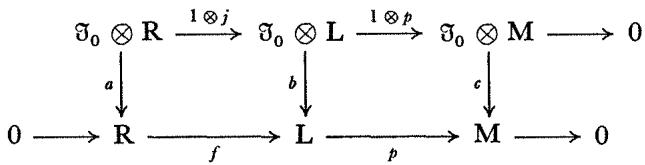
\includegraphics[keepaspectratio]{images/part003_24c814e1.jpg}}

其中 \(j\) 是典范单射， \(a, b, c\) 由典范单射 \(\mathfrak{I}_0 \to \mathbf{A}\) 导出（ \(\S 3\) , 第 4 号, 命题 4）；要证明的是 \(a\) 为满射。注意，由于 \(\mathbf{L}\) 是自由的， \(b\) 是单射的（ \(\S 3\) , 第 7 号, 命题 7 的推论 6），且 \(c\) 按假设是单射的。令 \(t\) 是 \(\mathbf{R}\) 的一个元素， \(t\) 是它在 \(\mathbf{R} / \mathfrak{I}_0\mathbf{R}\) 中的类；则有一个正合序列（ \(\S 3\) , 第 6 号, 命题 5 及命题 6 的推论 2）

\[
\mathrm{R} / \mathfrak {I} _ {0} \mathrm{R} \xrightarrow {\jmath} \mathrm{L} / \mathfrak {I} _ {0} \mathrm{L} \xrightarrow {\bar {p}} \mathrm{M} / \mathfrak {I} _ {0} \mathrm{M} \longrightarrow 0
\]

其中 \(j\) 和 \(\bar{p}\) 是 \(j\) 与 \(p\) 过渡到商时导出的，而 \(\bar{p}\) 按假设是双射；于是 \(\bar{j}(t) = 0\) ，换言之 \(j(t) \in \mathfrak{I}_0\mathbf{L}\) 。则存在一个元素 \(z \in \mathfrak{I}_0 \otimes \mathbf{L}\) 使得 \(j(t) = b(z)\) ；由于 \(p(b(z)) = 0\) ，有 \(c((1 \otimes p)(z)) = 0\) ，又由于 \(c\) 是单射，有 \((1 \otimes p)(z) = 0\) 。换言之， \(z\) 是某个元素 \(t' \in \mathfrak{I}_0 \otimes \mathbf{R}\) 在 \(1 \otimes j\) 下的像，于是 \(j(a(t')) = b(z) = j(t)\) ；由于 \(j\) 是单射，这就蕴含 \(t = a(t')\) 。

我们将在后文（交换代数, II, §3, 第 2 号, 命题 5）中说明如何把这命题推广到非分次模。

引理1. 交换群 \(\Delta\) 使得在 \(\Delta\) 上存在一个与 \(\Delta\) 的群结构相容的全序，其必要且充分的条件是 \(\Delta\) 无挠。

若在 \(\Delta\) 上存在这样一个序结构，且若 \(\lambda > 0\) ，则 \(\lambda + \mu > 0\) （对所有 \(\mu \geqslant 0\) ），特别地，对整数 \(n > 0\) 作归纳得 \(n.\lambda > 0\) ，这就证明 \(\Delta\) 是无挠的（因为每个元素 \(\neq 0\) （ \(\Delta\) 中的）或者 \(>0\) 或者 \(< 0\) ）。反之，若 \(\Delta\) 是无挠的，则 \(\Delta\) 是一个向量 \(\mathbf{Z}\) -空间的子 \(\mathbf{Q}\) -模（ \(\S 7\) , 第 10 号, 命题 26 的推论 1），可设它具有形式 \(\mathbf{Q}^{(I)}\) ；若给 I 一个良序（集合论, III, \(\S 2\) , 第 3 号, 定理 1），并给 \(\mathbf{Q}\) 其通常的序，则集合 \(\mathbf{Q}^{(I)}\) 赋予字典序是全序的（集合论, III, \(\S 2\) , 第 6 号）；立即看出这个序与 \(\mathbf{Q}^{(I)}\) 的加法群结构相容。

命题8. 设 \(\Delta\) 是一个无挠交换群，A 是一个类型为 \(\Delta\) 的分次环。若 A 中两个齐次元素 \(\neq 0\) 的乘积 \(\neq 0\) ，则环 A 没有零因子。

设 \(\Delta\) 被赋予与其群结构相容的全序（引理

\begin{enumerate}
\def\labelenumi{\arabic{enumi})}
\tightlist
\item
  ，并设 \(x = \sum_{\lambda \in \Delta} x_{\lambda}, y = \sum_{\lambda \in \Delta} y_{\lambda}\) 是 A 的两个非零元素（ \(x_{\lambda}\) 和 \(y_{\lambda}\) 是次数为 \(\lambda\) 的齐次元素，对所有 \(\lambda \in \Delta\) ）；设 \(\alpha\) （相应地， \(\beta\) ）是元素 \(\lambda \in \Delta\) （使 \(x_{\lambda} \neq 0\) （相应地， \(y_{\lambda} \neq 0\) ）者）中最大的；立即看出，若 \(\lambda \neq \alpha\) 或 \(\mu \neq \beta\) ，则或者 \(x_{\lambda}y_{\mu} = 0\) 或者 \(\deg(x_{\lambda}y_{\mu}) < \alpha + \beta\) ；因此 \(xy\) 的次数为 \(\alpha + \beta\) 的齐次分量是 \(x_{\alpha}y_{\beta}\) ，它按假设非零；从而 \(xy \neq 0\) 。
\end{enumerate}

\subsection{分次模的分次张量积}

设 \(\Delta\) 是一个交换幺半群，其单位元记作 0，A 是一个类型为 \(\Delta\) 的分次环，M（相应地，N）是一个类型为 \(\Delta\) 的分次右（相应地，左）A-模。设 \((\mathbf{A}_{\lambda})\) （相应地， \((\mathbf{M}_{\lambda}), (\mathbf{N}_{\lambda}))\) ）是 A（相应地，M，N）的分次；Z-模 M 和 N 的张量积 \(\mathbf{M} \otimes_{\mathbf{Z}} \mathbf{N}\) 是诸 \(\mathbf{M}_{\lambda} \otimes_{\mathbf{Z}} \mathbf{N}_{\mu}\) 的直和（§3, 第 7 号, 命题 7），因而后者构成这个 Z-模上类型为 \(\Delta, \Delta\) 的一个双分次。考虑 M \(\otimes_{\mathbf{Z}} \mathbf{N}\) 上与这个双分次相关联的类型为 \(\Delta\) 的全分次（第 1 号，例 4）；它由子 Z-模 \(\mathrm{P}_{\lambda} = \sum_{\mu + v = \lambda} (\mathrm{M}_{\mu} \otimes_{\mathbf{z}} \mathrm{N}_{v})\) 组成。已知 Z-模 M \(\otimes_{\mathbf{A}} \mathbf{N}\) 是 M \(\otimes_{\mathbf{Z}} \mathbf{N}\) 关于由元素 \((xa) \otimes y - x \otimes (ay)\) （其中 \(x \in \mathbf{M}, y \in \mathbf{N}\) 和 \(a \in \mathbf{A}\) ，§3, 第 1 号）生成的子 Z-模 Q 的商；如果对所有 \(\lambda \in \Delta\) , \(x_{\lambda}, y_{\lambda}, a_{\lambda}\) 分别是次数为 \(\lambda\) 的齐次分量（ \(x, y, a\) 的），则显然 \((xa) \otimes y - x \otimes (zy)\) 是齐次元素 \((x_{\lambda}a_{v}) \otimes y_{\mu} - x_{\lambda} \otimes (a_{v}y_{\mu})\) 之和，换言之，Q 是 M \(\otimes_{\mathbf{Z}} \mathbf{N}\) 的一个分次子 Z-模（第 3 号, 命题 2），且商

\[
\mathbf {M} \otimes_ {\mathbf {A}} \mathbf {N} = (\mathbf {M} \otimes_ {\mathbf {Z}} \mathbf {N}) / \mathbf {Q}
\]

因此典范地具有一个类型为 \(\Delta\) 的分次 Z-模结构（第 3 号）。此外（第 3 号, 命题 5），A 的中心 C 是 A 的一个分次子环；我们刚在 M \(\otimes_{\mathbf{A}} \mathbf{N}\) 上定义的这个分次与其在分次环 C 上的模结构相容。因为 M \(\otimes_{\mathbf{Z}} \mathbf{N}\) 典范地具有两个 C-模结构，对于它们分别有 \(c(x \otimes y) = (xc) \otimes y\) 和 \((x \otimes y)c = x \otimes (cy)\) （对 \(x \in \mathbf{M}, y \in \mathbf{N}, c \in \mathbf{C}\) ）（ \(\S 3\) , 第 3 号）；若 \(x \in \mathbf{M}_{\lambda}, y \in \mathbf{N}_{\mu}, c \in \mathbf{C} \cap \mathbf{A}_{\nu}\) ，则两个元素 \(c(x \otimes y)\) 和 \((x \otimes y)c\) 属于 (M \(\otimes_{\mathbf{Z}} \mathbf{N})_{\lambda + \mu + \nu}\) ，且它们的差属于 Q，因此它们在 M \(\otimes_{\mathbf{A}} \mathbf{N}\) 中的共同像属于 (M \(\otimes_{\mathbf{A}} \mathbf{N})_{\lambda + \mu + \nu}\) ，这便确立了我们的断言。当我们把 M \(\otimes_{\mathbf{A}} \mathbf{N}\) 作为分次 C-模谈论时，除非另有说明，总是指如此定义的结构。注意 (M \(\otimes_{\mathbf{A}} \mathbf{N})_{\lambda}\) 可以定义为 M \(\otimes_{\mathbf{A}} \mathbf{N}\) 的由诸 \(x_{\mu} \otimes y_{\nu}\) （其中 \(x_{\mu} \in \mathbf{M}_{\mu}, y_{\nu} \in \mathbf{N}_{\nu}\) 且 \(\mu + \nu = \lambda\) ）生成的加法子群。

设 \(\mathbf{M}'\) （相应地， \(\mathbf{N}'\) ）是另一个分次右（相应地，左）A-模，且 \(u: \mathbf{M} \to \mathbf{M}', v: \mathbf{N} \to \mathbf{N}'\) 是次数分别为 \(\alpha\) 和 \(\beta\) 的分次同态。那么由上述注记立即得出 \(u \otimes v\) 是次数为 \(\alpha + \beta\) 的分次（C-模）同态。

当A是交换环时，在任意有限多个分次A-模的张量积上同样可以定义与A-模结构相容的分次结构；此外，显然诸如结合性同构 \((\mathbf{M} \otimes \mathbf{N}) \otimes \mathbf{P} \to \mathbf{M} \otimes (\mathbf{N} \otimes \mathbf{P})\) (§ 3，第 8 号，命题 8)是分次模的同构。

注. 当 A 具有平凡分次（第 1 号，例 1）时， \((\mathbf{M} \otimes_{\mathbf{A}} \mathbf{N})_{\lambda}\) 就是诸子 Y-模 \(\mathbf{M}_{\mu} \otimes_{\mathbf{A}} \mathbf{N}_{\nu}\) （ \(\mathbf{M} \otimes_{\mathbf{A}} \mathbf{N}\) 中的，满足 \(\mu + \nu = \lambda\) ）的直和。

设 M（相应地，N）是类型为 \(\Delta\) 的分次右（相应地，左）A-模，P 是类型为 \(\Delta\) 的分次 Z-模，并设 f 是 \(M \times N\) 到 P 中的一个 Z-双线性映射，它满足 §3, 第 1 号的条件 (1)，且此外使得

\[
f (x _ {\lambda}, y _ {\mu}) \in \mathrm{P} _ {\lambda + \mu} \quad \text { for } x _ {\lambda} \in \mathrm{M} _ {\lambda}, y _ {\mu} \in \mathrm{N} _ {\mu}, \lambda , \mu \text { in } \Delta .
\]

那么 \(f(x, y) = g(x \otimes y)\) ，其中 \(g: \mathbf{M} \otimes_{\mathbf{A}} \mathbf{N} \to \mathbf{P}\) 是一个 \(\mathbf{Z}\) -线性映射（§3, 第 1 号, 命题 1），且由上述条件可知 \(g\) 是次数为 0 的分次 \(\mathbf{Z}\) -模同态。

设 B 是另一个类型为 \(\Delta\) 的分次环， \(\rho: A \to B\) 是分次环的一个同态（第 2 号）；则 \(\rho_*(B_d)\) 是类型为 \(\Delta\) 的一个分次右 A-模。若 E 是类型为 \(\Delta\) 的分次左 A-模，且给 \(\rho^*(B_d) \otimes_A E\) 赋予上面定义的类型为 \(\Delta\) 的分次 Z-模结构，则典范的左 B-模结构（ \(\S\) 5, 第 1 号）与

\[
\mathbf {E} _ {(\mathbf {B})} = \rho^ {*} (\mathbf {E}) = \rho_ {*} (\mathbf {B} _ {d}) \otimes_ {\mathbf {A}} \mathbf {E}.
\]

的分次相容。这样得到的分次 B-模称为借助 \(\rho\) 把纯量环扩张到 B 而得到的；当我们把 \(\mathrm{E}_{(\mathrm{B})}\) 或 \(\rho^{*}(\mathrm{E})\) 作为分次 B-模谈论时，除非另有说明，总是指这一结构。

\subsection{分次同态的分次模}

我们在本号中假设幺半群 \(\Delta\) 是一个群。设 A 是类型为 \(\Delta\) 的分次环，M、N 是两个类型为 \(\Delta\) 的分次左（例如）A-模。设 H \(_{\lambda}\) 表示由 M 到 N 的次数为 \(\lambda\) 的分次同态构成的加法群（第 2 号）；在 M 到 N 的所有同态（带非分次 A-模结构）的加法群 Hom \(_{A}\) (M, N) 中，对 \(\lambda \in \Delta\) 的诸 H \(_{\lambda}\) 之和是直和。因为，若有一个关系 \(\sum_{\lambda} u_{\lambda} = 0\) ，其中 \(u_{\lambda} \in \mathrm{H}_{\lambda}\) （对所有 \(\lambda\) ），则由此得出 \(\sum_{\lambda} u_{\lambda}(x_{\mu}) = 0\) （对所有 \(\mu\) 及所有 \(x_{\mu} \in \mathrm{M}_{\mu}\) ）。由于 \(\Delta\) 的元素都可消去， \(u_{\lambda}(x_{\mu})\) 是 \(\sum_{\lambda} u_{\lambda}(x_{\mu})\) 的次数为 \(\lambda + \mu\) 的齐次分量；因此 \(u_{\lambda}(x_{\mu}) = 0\) （对每个有序对 ( \(\mu, \lambda\) ) 及每个 \(x_{\mu} \in \mathrm{M}_{\mu}\) ），这蕴含 \(u_{\lambda} = 0\) （对所有 \(\lambda \in \Delta\) ）。我们（在本段中）用 Homgr \(_{A}\) (M, N) 表示 Hom \(_{A}\) (M, N) 的加法子群，即所有 H \(_{\lambda}\) 的和，并称之为从 M 到 N 的分次 A-模同态的加法群。设 C 为 A 的中心，它是一个分次子环（第 3 号，命题 5 的推论）；对于 \(\mathrm{Hom}_{\mathbf{A}}(\mathbf{M},\mathbf{N})\) 上的典范 C-模结构（§ 1，第 14 号，注记 1）， \(\mathrm{Homgr}_{\mathbf{A}}(\mathbf{M},\mathbf{N})\) 是一个子模，且分次 \((\mathbf{H}_{\lambda})\) 与 C-模结构相容：因为，若 \(c_{\nu}\in \mathbf{C}\cap \mathbf{A}_{\nu}\) , \(x_{\mu}\in \mathbf{N}_{\mu}\) 和 \(u_{\lambda}\in \mathbf{H}_{\lambda}\) ，则由定义 \((c_{\nu}u_{\lambda})(x_{\mu}) = c_{\nu}.u_{\lambda}(x_{\mu})\subset \mathbf{N}_{\lambda +\mu +\nu}\) ，因此 \(c_{\nu}u_{\lambda}\in \mathbf{H}_{\lambda +\nu}\) .

设 \(\mathbf{M}'\) 和 \(\mathbf{N}'\) 是两个类型为 \(\Delta\) 的分次左 A-模，且 \(u':\mathbf{M}'\to\mathbf{M}\) , \(v':\mathbf{N}\to\mathbf{N}'\) 是次数分别为 \(\alpha\) 和 \(\beta\) 的分次同态。那么立即看出 \(\operatorname{Hom}(u',v')\colon w\mapsto v'\circ w\circ u'\) 把 \(\operatorname{Homgr}_{\mathbf{A}}(\mathbf{M},\mathbf{N})\) 映到 \(\operatorname{Homgr}_{\mathbf{A}}(\mathbf{M}',\mathbf{N}')\) 中，且它到 \(\operatorname{Homgr}_{\mathbf{A}}(\mathbf{M},\mathbf{N})\) 的限制是到 \(\operatorname{Homgr}_{\mathbf{A}}(\mathbf{M}',\mathbf{N}')\) 中的次数为 \(\alpha+\beta\) 的分次同态。

特别地， \(\operatorname{Homgr}_{\mathbf{A}}(\mathbf{M}, \mathbf{M})\) 是 \(\operatorname{End}_{\mathbf{A}}(\mathbf{M})\) 的一个分次子环，记作 \(\operatorname{Endgr}_{\mathbf{A}}(\mathbf{M})\) 。

注. 若 M 和 N 是分次左 A-模， \(\operatorname{Homgr}_{\mathbf{A}}(\mathbf{M}, \mathbf{N})\) 一般不同于 \(\operatorname{Hom}_{\mathbf{A}}(\mathbf{M}, \mathbf{N})\) 。然而当 M 是有限生成的 A-模时，这两个集合相等。因为此时 M 由有限个齐次元素 \(x_{i}\) （ \(1 \leqslant i \leqslant n\) ）生成；设 \(d(i)\) 是 \(x_{i}\) 的次数；令 \(u \in \operatorname{Hom}_{\mathbf{A}}(\mathbf{M}, \mathbf{N})\) ，且对所有 \(\lambda \in \Delta\) ，设 \(z_{i,\lambda}\) 表示 \(u(x_{i})\) 的次数为 \(\lambda + d(i)\) 的齐次分量。我们证明存在一个同态 \(u_{\lambda}: \mathbf{M} \to \mathbf{N}\) ，使得 \(u_{\lambda}(x_{i}) = z_{i,\lambda}\) （对所有 \(i\) ）。只需证明若 \(\sum_{i} a_{i} x_{i} = 0\) ，其中 \(a_{i} \in \mathbf{A}\) （对于 \(1 \leqslant i \leqslant n\) ），则 \(\sum_{i} a_{i} z_{i,\lambda} = 0\) （对所有 \(\lambda \in \Delta\) ）（§1, 第 7 号, 注）。可以假设每个 \(a_{i}\) 都是次数为 \(d'(i)\) 的齐次元素，使得 \(d(i) + d'(i) = \mu\) （对所有 \(i\) ）（第 3 号, 注 1）；则 \(\sum_{i} a_{i} u(x_{i}) = 0\) ；在左边取次数为 \(\lambda + \mu\) 的齐次分量，我们得到 \(\sum_{i} a_{i} z_{i,\lambda} = 0\) ，由此得出同态 \(u_{\lambda}\) 的存在性；此外显然 \(u_{\lambda}\) 是次数为 \(\lambda\) 的分次同态。最后， \(u_{\lambda} = 0\) （除 \(\lambda\) 的有限多个值外），且按定义 \(u = \sum_{\lambda} u_{\lambda}\) ，这就证明了我们的断言。

特别地， \(\operatorname{Homgr}_{\mathbf{A}}(\mathbf{A}_s, \mathbf{M}) = \operatorname{Hom}_{\mathbf{A}}(\mathbf{A}_s, \mathbf{M})\) （对每个分次左 A-模 M）；此外 \(\operatorname{Hom}_{\mathbf{A}}(\mathbf{A}_s, \mathbf{M})\) 具有一个分次左 A-模结构（而不仅仅是分次 C-模结构），且显然在此结构下，M 到 \(\operatorname{Hom}_{\mathbf{A}}(\mathbf{A}_s, \mathbf{M})\) 中的典范映射（ \(\S 1\) , 第 14 号, 注 2）是一个分次 A-模同构。

类似地， \(\operatorname{Homgr}_{\mathbf{A}}(\mathbf{M}, \mathbf{A}_s)\) 具有一个分次右 A-模结构（而不仅仅是分次 C-模结构）；它称为分次 A-模 M 的分次对偶，记作 \(\mathbf{M}^{*\mathbf{gr}}\) ，或当不会引起混淆时简记作 \(\mathbf{M}^*\) 。如果 \(u: \mathbf{M} \to \mathbf{N}\) 是次数为 \(\delta\) 的分次同态，则由上述可知，到 \(\mathbf{N}^{*\mathbf{gr}}\) 上的 \(^t u = \operatorname{Hom}(u, 1_{\mathbf{A}_s})\) 的限制，是分次对偶 \(\mathbf{N}^{*\mathbf{gr}}\) 到分次对偶 \(\mathbf{M}^{*\mathbf{gr}}\) 中的一个次数为 \(\delta\) 的分次同态，称为 \(u\) 的分次转置。

我们有时在分次对偶 \(M^{*gr}\) 上考虑借助同构 \(\lambda\mapsto-\lambda\) （ \(\Delta\) 的）从上述分次导出的分次（第 1 号，例 2），使得次数为 \(\lambda\) 的齐次元素（ \(M^{*gr}\) 中的）是 M 上次数为 \(-\lambda\) 的分次线性形式（当 A 具有平凡分次时，这些是在 \(M_{\mu}\) （指标 \(\mu\neq\lambda\) 的）上为零的线性形式）。那么，若 \(u:M\to N\) 是次数为 \(\delta\) 的分次同态，则 \(u'\) 成为次数为 \(-\delta\) 的分次同态。

设 A 是交换的且类型为 \(\Delta\) 的分次环，且设 M、N、P、Q 是四个类型为 \(\Delta\) 的分次 A-模。则存在次数为 0 的典范分次同态

\begin{enumerate}
\def\labelenumi{(\arabic{enumi})}
\setcounter{enumi}{2}
\tightlist
\item
\end{enumerate}

\[
\operatorname{Homgr} _ {\mathbf {A}} (\mathbf {M}, \operatorname{Homgr} _ {\mathbf {A}} (\mathbf {N}, \mathbf {P})) \rightarrow \operatorname{Homgr} _ {\mathbf {A}} (\mathbf {M} \otimes_ {\mathbf {A}} \mathbf {N}, \mathbf {P})\tag{4}
\]

\[
\operatorname{Homgr} _ {\mathbf {A}} (\mathbf {M}, \mathbf {N}) \otimes_ {\mathbf {A}} \mathrm{P} \rightarrow \operatorname{Homgr} _ {\mathbf {A}} (\mathbf {M}, \mathbf {N} \otimes_ {\mathbf {A}} \mathrm{P})
\]

\[
\operatorname{Homgr} _ {\mathbf {A}} (\mathbf {M}, \mathbf {P}) \otimes_ {\mathbf {A}} \operatorname{Homgr} _ {\mathbf {A}} (\mathbf {N}, \mathbf {Q}) \rightarrow \operatorname{Homgr} _ {\mathbf {A}} (\mathbf {M} \otimes_ {\mathbf {A}} \mathbf {N}, \mathbf {P} \otimes_ {\mathbf {A}} \mathbf {Q}) \tag {5}
\]

（张量积赋予第 5 号中所定义的分次），它们由限制 §4, 第 1、2、4 号中所定义的典范同态而得到；事实上，若 \(u: \mathbf{M} \to \operatorname{Homgr}_{\mathbf{A}}(\mathbf{N}, \mathbf{P})\) 是次数为 \(\delta\) 的分次同态，那么对所有 \(x \in \mathbf{M}_{\lambda}\) , \(u(x)\) 是 \(\mathbf{N} \to \mathbf{P}\) 的次数为 \(\delta + \lambda\) 的分次同态，因此对于 \(y \in \mathbf{N}_{\mu}\) , \(u(x)(y) \in \mathbf{P}_{\delta + \lambda + \mu}\) ；若 \(v: \mathbf{M} \otimes_{\mathbf{A}} \mathbf{N} \to \mathbf{P}\) 典范地对应于 \(u\) ，则于是看出 \(v\) 是次数为 \(\delta\) 的分次同态，由此得出关于 (3) 的断言；此外还可看出这个同态是双射。对 (4) 和 (5) 的论证类似。

特别地，若 \(\mathbf{P} = \mathbf{Q} = \mathbf{A}\) 在(5)中，则存在一个次数为0的典范分次同态

\[
\mathbf {M} ^ {* \mathrm{gr}} \otimes_ {\mathbf {A}} \mathbf {N} ^ {* \mathrm{gr}} \rightarrow (\mathbf {M} \otimes_ {\mathbf {A}} \mathbf {N}) ^ {* \mathrm{gr}}.\tag{6}
\]

\BourbakiAppendixSection{伪模}

\subsection{向伪环添加单位元}

设 A 是一个伪环（I, §8, 第 1 号）。在集合 \(\mathbf{A}' = \mathbf{Z} \times \mathbf{A}\) 上，我们定义以下合成律：

\[
\left\{ \begin{array}{l} (m, a) + (n, b) = (m + n, a + b) \\ (m, a) (n, b) = (m n, m b + n a + a b). \end{array} \right.\tag{1}
\]

立即验证可知，A' 带这两个合成律是一个环，其中元素 \((1,0)\) 是单位元。集合 \(\{0\} \times A\) 是 A' 的一个双边理想，且 \(\iota: x \mapsto (0, x)\) 是伪环 A 到子伪环 \(\{0\} \times A\) 上的一个同构，借助它，A 与 \(\{0\} \times A\) 等同。A' 称为由伪环 A 添加单位元而导出的环。

如果 A 已经有一个单位元 \(\varepsilon\) ，则元素 \(e = (0, \varepsilon)\) （ \(\mathbf{A}'\) 中的）是属于 \(\mathbf{A}'\) 的中心的一个幂等元，且使得

\[
\mathrm{A} = e \mathrm{A} ^ {\prime} = \mathrm{A} ^ {\prime} e.
\]

则 \((e\mathbf{A}', (1 - e)\mathbf{A}')\) 是（I, §8, 第 11 号意义下的） \(\mathbf{A}'\) 的一个直和分解，且环 \((1 - e)\mathbf{A}'\) 同构于 \(\mathbf{Z}\) 。

\subsection{伪模}

给定一个含或不含单位元的伪环 A，A 上的左伪模是一个交换群 E（加法记法），它以 A 为算子集，且满足 §1, 第 1 号, 定义 1 的公理 \((\mathbf{M}_{\mathrm{I}})\) , \((\mathbf{M}_{\mathrm{II}})\) 和 \((\mathbf{M}_{\mathrm{III}})\) 。A 上的右伪模类似地定义。

设 \(A'\) 是给 A 添加单位元所得的环。若 E 是 A 上的一个左伪模，则在 E 上关联一个左 \(A'\) -模结构，其方式是对所有 \(x \in E\) 及每个元素 \((n, a) \in A'\) ，写下

\[
(n, a). x = n x + a x.\tag{2}
\]

公理 \((\mathbf{M}_{\mathrm{I}})\) 到 \((\mathbf{M}_{\mathrm{IV}})\) （§1, 第 1 号, 定义 1 的）立即得到验证；此外，把这个模结构的算子集限制到 \(\{0\} \times A\) （与 A 等同）上，我们就在 E 上重新得到最初给定的伪模结构。

对于 E 的子集 M，要使 M 成为伪模 E 的带算子子群（此时诱导结构显然也是 A 上的左伪模结构），当且仅当 M 是相伴 A'-模 E 的子模，且此子 A'-模与伪模 M 相伴。进而，商 A'-模 E/M 与带算子商群 E/M 相伴，而后者显然是 A 上的伪模。

若 E、F 是 A 上的两个伪模，则带算子群同态 \(E \rightarrow F\) 与分别相伴于伪模 E 和 F 的 A'-模之间的 A'-线性映射 \(E \rightarrow F\) 完全相同。若 \((\mathbf{E}_{t})_{t \in I}\) 是 A 上的一族伪模，则带算子群 \(\prod_{i\in I}E\) 和 \(\bigoplus_{i\in I}E_{i}\) 是 A 上的伪模，且相伴的 A'-模分别是相伴 A'-模 \(E_{i}\) 的积与直和。对伪模的逆极限与直极限也有类似的结果。因此，A 上伪模的理论可以完全归结为 A'-模的理论。

\BourbakiExercisesHeading
% semantic-fragments: legacy-input-seam
\relax{}
\BourbakiExercisesSection

\begin{enumerate}
\def\labelenumi{\arabic{enumi}.}
\item
  设 E, F 为两个 A-模，且 \(u: \mathbf{E} \to \mathbf{F}\) 为线性映射。设 M 为 E 的子模，N 为 F 的子模， \(i: \mathbf{M} \to \mathbf{E}\) 为典范单射， \(q: \mathbf{F} \to \mathbf{F} / \mathbf{N}\) 为典范满射。证明 \(u(\mathbf{M}) = \operatorname{Im}(u \circ i)\) 和 \(u^{-1}(\mathbf{N}) = \operatorname{Ker}(q \circ u)\) .
\item
  设 E 为左 A-模；对于 A 的每个左理想 a，令 aE 表示所有 ax 的和，其中 \(x \in E\) ，因此它是 E 的子模。
\end{enumerate}

\begin{enumerate}
\def\labelenumi{(\alph{enumi})}
\item
  证明对于每个 A-模族 \((\mathbf{E}_{\lambda})_{\lambda \in L}\) ，a. \(\bigoplus_{\lambda \in L} \mathbf{E}_{\lambda}\) 典范地等同于 \(\bigoplus_{\lambda \in L} a E_{\lambda}\) .
\item
  若 \(\mathfrak{a}\) 是 \(\mathbf{A}\) 的有限生成左理想，证明对每个族 \((\mathbf{E}_{\lambda})_{\lambda \in L}\) （由 \(\mathbf{A}\) -模组成）， \(\mathfrak{a}\) . \(\prod_{\lambda \in L} \mathbf{E}_{\lambda}\) 典范地等同于 \(\prod_{\lambda \in L} \mathfrak{a}\mathbf{E}_{\lambda}\) 。给出一个例子，其中 \(\mathfrak{a}\) 不是有限生成的且上述性质不成立（取 \(\mathbf{A}\) 交换且所有 \(\mathbf{E}_{\lambda}\) 都等于 \(\mathbf{A}\) ）.
\end{enumerate}

*(c) 设 K 是一个交换域，A 是 K 上两个未定元的多项式环 K{[}X,Y{]} ，m = AX 且 n = AY。若 E 是 \(\mathbf{A}^2\) 关于 \(\mathbf{A}^2\) 中由 \(\mathbf{Xe}_1 - \mathbf{Ye}_2\) 生成的子模的商 A-模 (其中 \((e_1, e_2)\) 是 \(\mathbf{A}^2\) 的典范基 )，证明 \((m \cap n)E \neq (mE) \cap (nE)\) .*

\begin{enumerate}
\def\labelenumi{\arabic{enumi}.}
\setcounter{enumi}{2}
\tightlist
\item
  设 E 是一个 A-模。
\end{enumerate}

\begin{enumerate}
\def\labelenumi{(\alph{enumi})}
\tightlist
\item
  设 \((\mathbf{L}_{\mu})_{\mu \in \mathbf{M}}\) 是一族右有向有序集，且对所有 \(\mu \in \mathbf{M}\) ，设 \((\mathrm{F}_{\lambda \mu})_{\lambda \in L_{\mu}}\) 是 \(\mathbf{E}\) 的一族递增的子模。证明
\end{enumerate}

\[
\bigcap_ {\mu \in \mathbf {M}} \left(\sum_ {\lambda \in L _ {\mu}} F _ {\lambda \mu}\right) = \sum_ {\rho \in \prod_ {\mu} L _ {\mu}} \left(\bigcap_ {\mu \in \mathbf {M}} F _ {\rho (\mu), \mu}\right).
\]

\begin{enumerate}
\def\labelenumi{(\alph{enumi})}
\setcounter{enumi}{1}
\tightlist
\item
  设 A 为一个域，E 为 A-模 \(A^{N}\) ；设 G 为 E 的子模 \(\mathbf{A}^{(\mathbf{N})}\) ；另一方面，对 N 的每个有限子集 H，设 \(F_{H}\) 为子模 \(\prod_{n\in \mathbf{N}}\mathbf{M}_n\) （ \(\mathbf{E}\) 的），其中 \(\mathbf{M}_n = \mathbf{A}\) （对于 \(n\notin \mathrm{H}\) ）且 \(\mathbf{M}_n = 0\) （对于 \(n\in \mathrm{H}\) ）。证明族 \((\mathrm{F_H})\) （其中 \(\mathbf{H}\) 遍历集 \(\Phi\) ，由 \(\mathbf{N}\) 的有限子集组成）是右有向的，并且
\end{enumerate}

\[
\left(\bigcap_ {\mathrm{H} \in \Phi} \mathrm{F} _ {\mathrm{H}}\right) + \mathrm{G} \neq \bigcap_ {\mathrm{H} \in \Phi} (\mathrm{F} _ {\mathrm{H}} + \mathrm{G}).
\]

\begin{enumerate}
\def\labelenumi{\arabic{enumi}.}
\setcounter{enumi}{3}
\tightlist
\item
  设 \(\mathbf{E}, \mathbf{F}_1, \mathbf{F}_2\) 为三个 A-模， \(f_1: \mathbf{F}_1 \to \mathbf{E}\) , \(f_2: \mathbf{F}_2 \to \mathbf{E}\) 为两个 A-线性映射。 \(\mathbf{F}_1\) 和 \(\mathbf{F}_2\) 相对于 \(f_1\) 和 \(f_2\) 的纤维积是积 \(\mathbf{F}_1 \times \mathbf{F}_2\) 中由有序对 \((x_1, x_2)\) （满足 \(f_1(x_1) = f_2(x_2)\) ）组成的子模；记作 \(\mathbf{F}_1 \times_{\mathbf{E}} \mathbf{F}_2\) .
\end{enumerate}

\begin{enumerate}
\def\labelenumi{(\alph{enumi})}
\item
  对于每一对 A-线性映射 \(u_1 \colon G \to F_1, u_2 \colon G \to F_2\) （满足 \(f_1 \circ u_1 = f_2 \circ u_2\) ），存在且仅存在一个 A-线性映射 \(u \colon G \to F_1 \times_E F_2\) ，使得 \(p_1 \circ u = u_1, p_2 \circ u = u_2\) ，其中 \(p_1\) 和 \(p_2\) 表示 \(F_1 \times_E F_2\) 上投影 \(pr_1\) 和 \(pr_2\) 的限制.
\item
  设 \(\mathbf{E}'\) , \(\mathbf{F}_1'\) , \(\mathbf{F}_2'\) 是三个A-模， \(f_1': \mathbf{F}_1' \to \mathbf{E}', f_2': \mathbf{F}_2' \to \mathbf{E}'\) 为两个 A-线性映射，而 \(\mathbf{F}_1' \times_{\mathbf{E}'} \mathbf{F}_2'\) 为相对于这些映射的纤维积。对于每一组 A-线性映射 \(v_1: \mathbf{F}_1 \to \mathbf{F}_1'\) , \(v_2: \mathbf{F}_2 \to \mathbf{F}_2'\) , \(w: \mathbf{E} \to \mathbf{E}'\) ，若 \(f_1' \circ v_1 = w \circ f_1, f_2' \circ v_2 = w \circ f_2\) ，设 \(v\) 是 \(\mathbf{F}_1 \times_{\mathbf{E}} \mathbf{F}_2\) 到 \(\mathbf{F}_1' \times_{\mathbf{E}'} \mathbf{F}_2'\) 的A-线性映射，对应于两个线性映射 \(v_1 \circ p_1\) 和 \(v_2 \circ p_2\) 。证明如果 \(v_1\) 和 \(v_2\) 是单射，则 \(v\) 也是单射；给出一个例子，其中 \(v_1\) 和 \(v_2\) 是满射但 \(v\) 不是满射（取 \(\mathbf{E}' = \{0\}\) ）。如果 \(w\) 是单射且 \(v_1\) 和 \(v_2\) 是满射，证明 \(v\) 是满射。
\end{enumerate}

\begin{enumerate}
\def\labelenumi{\arabic{enumi}.}
\setcounter{enumi}{4}
\tightlist
\item
  设 \(\mathbf{E}, \mathbf{F}_1, \mathbf{F}_2\) 为三个 A-模， \(f_1: \mathbf{E} \to \mathbf{F}_1, f_2: \mathbf{E} \to \mathbf{F}_2\) 为两个线性映射。 \(\mathbf{F}_1\) 和 \(\mathbf{F}_2\) 相对于 \(f_1\) 和 \(f_2\) 的融合和是 \(\mathbf{F}_1 \times \mathbf{F}_2\) 关于 \(\mathbf{E}\) 在映射 \(z \mapsto (f_1(z), -f_2(z))\) 下的像所成的子模的商模；记作 \(\mathbf{F}_1 \oplus_{\mathbf{E}} \mathbf{F}_2\) .
\end{enumerate}

\begin{enumerate}
\def\labelenumi{(\alph{enumi})}
\tightlist
\item
  对于每一对 A-线性映射 \(u_{1}: \mathbf{F}_{1} \to \mathbf{G}, u_{2}: \mathbf{F}_{2} \to \mathbf{G}\) ，若 \(u_{1} \circ f_{1} = u_{2} \circ f_{2}\) ，证明存在且仅存在一个 A-线性映射 \(u: \mathbf{F}_{1} \oplus_{\mathbf{E}} \mathbf{F}_{2} \to \mathbf{G}\) ，使得 \(u \circ j_{1} = u_{1}, u \circ j_{2} = u_{2}\) ，其中 \(j_{1}\) 和 \(j_{2}\) 分别表示典范映射
\end{enumerate}

\[
\mathbf {F} _ {1} \times \mathbf {F} _ {2} \rightarrow \mathbf {F} _ {1} \oplus_ {\mathrm{E}} \mathbf {F} _ {2}
\]

与典范单射 \(\mathbf{F}_1\to \mathbf{F}_1\times \mathbf{F}_2,\mathbf{F}_2\rightarrow \mathbf{F}_1\times \mathbf{F}_2.\)

\begin{enumerate}
\def\labelenumi{(\alph{enumi})}
\setcounter{enumi}{1}
\tightlist
\item
  设 \(\mathbf{E}'\) , \(\mathbf{F}_1'\) , \(\mathbf{F}_2'\) 是三个A-模， \(f_1': \mathbf{E}' \to \mathbf{F}_1'\) , \(f_2': \mathbf{E}' \to \mathbf{F}_2'\) 为两个 A-线性映射，而 \(\mathbf{F}_1' \oplus_{\mathbf{E}'} \mathbf{F}_2'\) 为相对于这些映射的融合和。对于每一组 A-线性映射 \(v_1: \mathbf{F}_1' \to \mathbf{F}_1\) , \(v_2: \mathbf{F}_2' \to \mathbf{F}_2\) , \(w: \mathbf{E}' \to \mathbf{E}\) ，若 \(v_1 \circ f_1' = f_1 \circ w\) , \(v_2 \circ f_2' = f_2 \circ w\) ，设 \(v\) 是 \(\mathbf{F}_1' \oplus_{\mathbf{E}'} \mathbf{F}_2'\) 到 \(\mathbf{F}_1 \oplus_{\mathbf{E}} \mathbf{F}_2\) 的A-线性映射，对应于两个线性映射 \(j_1 \circ v_1\) 和 \(j_2 \circ v_2\) 。证明如果 \(v_1\) 和 \(v_2\) 是满射，那么 \(v\) 也是满射；给出一个例子，其中 \(v_1\) 和 \(v_2\) 是单射但 \(v\) 不是单射。证明如果 \(w\) 是满射且 \(v_1\) 和 \(v_2\) 是单射，则 \(v\) 是单射。
\end{enumerate}

\begin{enumerate}
\def\labelenumi{\arabic{enumi}.}
\setcounter{enumi}{5}
\tightlist
\item
  给定一个 A-模 E，设 \(\gamma(E)\) 表示 E 的生成系的基数中的最小者。
\end{enumerate}

\begin{enumerate}
\def\labelenumi{(\alph{enumi})}
\tightlist
\item
  若 \(0 \to \mathbf{E} \to \mathbf{F} \to \mathbf{G} \to 0\) 是 A-模的正合序列，则
\end{enumerate}

\[
\gamma (\mathbf {G}) \leqslant \gamma (\mathbf {F}) \leqslant \gamma (\mathbf {E}) + \gamma (\mathbf {G}).
\]

给出一个乘积 \(\mathbf{F} = \mathbf{E} \times \mathbf{G}\) 的例子，使得 \(\gamma(\mathbf{E}) = \gamma(\mathbf{F}) = \gamma(\mathbf{G}) = 1\) （取 \(\mathbf{E}\) 和 \(\mathbf{G}\) 为 \(\mathbf{Z}\) 的商模 ）.

\begin{enumerate}
\def\labelenumi{(\alph{enumi})}
\setcounter{enumi}{1}
\item
  若 \(\mathbf{E}\) 是子模族 \((\mathrm{F}_{\lambda})_{\lambda \in L}\) 的和，则 \(\gamma (\mathbf{E})\leqslant \sum_{\lambda \in L}\gamma (\mathbf{F}_{\lambda}).\)
\item
  若 \(\mathbf{M}\) 和 \(\mathbf{N}\) 是模 \(\mathbf{E}\) 的子模，证明
\end{enumerate}

\[
\sup (\gamma (\mathbf {M}), \gamma (\mathbf {N})) \leqslant \gamma (\mathbf {M} \cap \mathbf {N}) + \gamma (\mathbf {M} + \mathbf {N}).
\]

\begin{enumerate}
\def\labelenumi{\arabic{enumi}.}
\setcounter{enumi}{6}
\tightlist
\item
  \begin{enumerate}
  \def\labelenumii{(\alph{enumii})}
  \tightlist
  \item
    设 A 为一个环，E 为一个 (A, A)-双模；在积 \(B = A \times E\) 上，通过令下式成立来定义环结构
  \end{enumerate}
\end{enumerate}

\[
(a, x) (a ^ {\prime}, x ^ {\prime}) = (a a ^ {\prime}, a x ^ {\prime} + x a ^ {\prime});
\]

E（典范地等同于 \(\{0\} \times \mathbf{E}\) ）于是是B的一个双边理想，使得 \(\mathbf{E}^2 = \{0\}\) .

\begin{enumerate}
\def\labelenumi{(\alph{enumi})}
\setcounter{enumi}{1}
\tightlist
\item
  通过适当选取 A 和 E，证明 E 可以是一个左 B-模，其 \(\gamma(\mathbf{E})\) （习题6）为任意基数，尽管 \(\gamma(\mathbf{B}_{s}) = 1\) .
\end{enumerate}

*8. 设 A 是一个交换环， \(\mathbf{B} = \mathbf{A}[\mathbf{X}_n]_{n\geqslant 1}\) 是 A 上含无穷多个未定元的多项式环，C 是 B 关于由多项式 \((\mathbf{X}_1 - \mathbf{X}_2)\mathbf{X}_i\) （对于 \(i\geqslant 3\) ）生成的理想的商环。若 \(\xi_1\) 和 \(\xi_2\) 分别是 \(\mathbf{X}_1\) 和 \(\mathbf{X}_2\) 在 C 中的类，证明单生成理想 \(\mathrm{C}\xi_1\) 和 \(\mathrm{C}\xi_2\) 在 C 中的交不是有限生成的理想。*

\begin{enumerate}
\def\labelenumi{\arabic{enumi}.}
\setcounter{enumi}{8}
\item
  证明：在 A-模 E 中，若 \((\mathrm{F}_{n})_{n\geqslant1}\) 是有限生成子模的一个严格递增序列，则以诸 \(F_{n}\) 之并为 E 的子模的 F 不是有限生成的。由此推出，如果 E 是一个非有限生成的 A-模，则存在 E 的一个子模 F，使得 \(\gamma(\mathrm{F})=\aleph_{0}(=\mathrm{Card}(\mathbf{N}))\) .
\item
  设 E 是一个 Z-模，它是两个子模 M、N 的直和，且分别同构于 Z/2Z 和 Z/3Z；证明：不存在将 E 分解为两个非零子模的直和的其他分解方式。
\item
  设 A 是具有左分式域 (I, § 9, 习题 15) 的环。证明在 A-模 \(A_{s}\) 中，异于 \(A_{s}\) 和 \(\{0\}\) 的子模没有互补子模（参见 I，§ 9，习题 16）。
\item
  设 \(\mathbf{G}\) 为一个模，且 \(\mathbf{E}, \mathbf{F}\) 为两个子模，使得 \(\mathbf{E} \subset \mathbf{F}\) .
\end{enumerate}

\begin{enumerate}
\def\labelenumi{(\alph{enumi})}
\item
  若 F 是 G 的直因子，则 F/E 是 G/E 的直因子。若同时 E 是 F 的直因子，则 E 是 G 的直因子。
\item
  若E是G的一个直因子，则E也是F的一个直因子。若进一步F/E是G/E的一个直因子，则F是G的一个直因子。
\item
  给出两个子模 \(\mathbf{M}, \mathbf{N}\) （ \(\mathbf{Z}\) -模 \(\mathbf{E} = \mathbf{Z}^2\) 的）的例子，使得 \(\mathbf{M}\) 和 \(\mathbf{N}\) 都是 \(\mathbf{E}\) 的直因子，但 \(\mathbf{M} + \mathbf{N}\) 不是 \(\mathbf{E}\) 的直因子.
\item
  设 \(p\) 是一个素数， \(U_p\) 是 \(\mathbf{Z}\) -模 \(\mathbf{Q} / \mathbf{Z}\) 的子模，由模 \(\mathbf{Z}\) 的类（对应于形如 \(k / p^n\) 的有理数）组成 ( \(k \in \mathbf{Z}\) , \(n \in \mathbf{N}\) )。设 \(E\) 为积 \(\mathbf{Z}\) -模 \(M \times N\) ，其中 \(M\) 和 \(N\) 都同构于 \(U_p\) ，且 \(M\) 和 \(N\) 被典范地等同于 \(E\) 的子模。考虑自同态 \(u: (x, y) \mapsto (x, y + px)\) （ \(E\) 的）；证明 \(u\) 是双射。若 \(M' = u(M)\) ，证明 \(M\) 和 \(M'\) 都是 \(E\) 的直因子，但 \(M \cap M'\) 不是 \(E\) 的直因子（利用 (b)，并证明 \(Z\) -模 \(U_p\) 除自身和 \{0\} 外没有其他直因子）.
\end{enumerate}

¶ 13. 设 E 是一个 A-模，B 为环 End\_A E。证明对于元素 \(u \in B\) ，以下三个条件等价：（1）Bu 是左 B-模 B\_s 的一个直因子；（2）uB 是右 B-模 B\_d 的一个直因子；（3）Ker(u) 和 Im(u) 是 A-模 E 的直因子。（注意，作为 B\_s 的直因子的每个左理想都具有 Bp 的形式，其中 p 是 E 中的一个投影算子；参见 I，§ 8，习题 12，并利用 II，§ 1，第 9 号，命题 15 的推论 1 和 2。）

\begin{enumerate}
\def\labelenumi{\arabic{enumi}.}
\setcounter{enumi}{13}
\tightlist
\item
  设 L 是一个良序集，E 是一个 A-模，且 \((\mathbf{E}_{\lambda})_{\lambda \in L}\) 是 E 的子模的一个递增族，使得：（1）存在 \(\lambda \in L\) 使得 \(E_{\lambda} = \{0\}\) ； (2) E 是诸 \(E_{\lambda}\) （ \(\lambda \in L\) ）的并； (3) 如果 \(\lambda \in L\) 使得 \(\mu < \lambda\) 的集合具有最大元 \(\lambda'\) , \(E_{\lambda}\) 是 \(E_{\lambda'}\) 与一个子模 \(F_{\lambda}\) 的直和；（4）若 \(\lambda \in L\) 是 \(\mu < \lambda\) 的集合的上确界，则 \(E_{\lambda}\) 是诸 \(E_{\mu}\) （ \(\mu < \lambda\) ）的并。在这些条件下，证明 E 是诸 \(F_{\lambda}\) 的直和。（用超限归纳法证明每个 \(E_{\lambda}\) 是诸 \(F_{\mu}\) 的直和，其中 \(\mu \leqslant \lambda\) 。)
\end{enumerate}

¶ 15. 设 c 为无限基数。

\begin{enumerate}
\def\labelenumi{(\alph{enumi})}
\item
  设 I 为一个集合， \(R\{a, b\}\) 为 I 的元素之间的一种关系，使得对所有 \(\alpha \in I\) ，由 \(\beta \in I\) 中使 \(R\{\alpha, \beta\}\) 成立者组成的集合具有基数 \(\leqslant c\) 。证明存在一个良序集 L 和 I 的子集的一个递增族 \((\mathrm{I}_{\lambda})_{\lambda \in L}\) ，使得：(1) 存在 \(\lambda \in L\) 使得 \(I_{\lambda} = \varnothing\) ；(2) I 是诸 \(I_{\lambda}\) （ \(\lambda \in L\) ）的并； (3) 如果 \(\lambda \in L\) 使得 \(\mu < \lambda\) 的集合有最大元 \(\lambda'\) , \(\text{Card}(\mathbf{I}_{\lambda} - \mathbf{I}_{\lambda'}) \leqslant c\) ；（4）若 \(\lambda \in L\) 是 \(\mu < \lambda\) 的集合的上确界，则 \(I_{\lambda}\) 是诸 \(I_{\mu}\) （ \(\mu < \lambda\) ）的并；(5) 若 \(\alpha \in I_{\lambda}\) 且 \(R\{\alpha, \beta\}\) 成立，则 \(\beta \in I_{\lambda}\) 。（首先注意，对所有 \(\alpha \in I\) ，由满足如下条件的 \(\beta \in I\) 组成的集合——存在一个整数 n 和一个由 I 的元素组成的序列 \((\gamma_{j})_{1 \leqslant j \leqslant n}\) ，使得 \(\gamma_{1} = \alpha, \gamma_{n} = \beta\) 且 \(R\{\gamma_{j}, \gamma_{j+1}\}\) 对 \(1 \leqslant j \leqslant n - 1\) 成立——具有基数 \(\leqslant c\) 。然后通过超限归纳法构造诸 \(I_{\lambda}\) 。）
\item
  设 E 是一个 A-模，它是子模族 \((\mathbf{M}_{\alpha})_{\alpha\in I}\) 的直和，使得 \(\gamma(\mathbf{M}_{\alpha})\leqslant c\) 对所有 \(\alpha\in I\) 成立（参见习题 6）。设 f 是 E 的一个自同态。证明存在一个良序集 L 和 I 的子集的一个递增族 \((\mathbf{I}_{\lambda})_{\lambda\in L}\) ，满足 (a) 中的性质 (1)、(2)、(3) 和 (4)，并且此外，若记 \(\mathbf{E}_{\lambda} = \bigoplus_{\alpha \in \mathbf{I}_{\lambda}} \mathbf{M}_{\alpha}\) ，则 \(f(\mathbf{E}_{\lambda}) \subset \mathbf{E}_{\lambda}\) 。（将 (a) 应用于关系 \(R\{\alpha, \beta\}\) ：“存在 \(x \in \mathbf{M}_{\alpha}\) 使得 \(f(x)\) 在 \(\mathbf{M}_{\beta}\) 中的分量 \(\neq 0\)”。）对所有满足下列条件的 \(\lambda \in \mathbf{L}\) ：\(\mu < \lambda\) 的集合有最大元 \(\lambda'\) ，记 \(\mathbf{F}_{\lambda} = \bigoplus_{\alpha \in \mathbf{I}_{\lambda} - \mathbf{I}_{\lambda'}} \mathbf{M}_{\alpha}\) 。证明 \(\mathbf{E}\) 是诸 \(\mathbf{F}_{\lambda}\) 的直和（应用习题 14）。
\item
  在 (b) 的假设和记号下，进一步假设 \(f\) 是一个投影算子，并记 \(\mathbf{P} = f(\mathbf{E})\) 。设 \(\mathbf{P}_{\lambda} = \mathbf{P} \cap \mathbf{E}_{\lambda}\) ；证明如果 \(\lambda \in \mathbf{L}\) 使得 \(\mu < \lambda\) 的集合有最大元 \(\lambda'\) , \(\mathbf{P}_{\lambda'}\) 是 \(\mathbf{P}_{\lambda}\) 的一个直因子（参见习题 12）， \(\mathbf{P}_{\lambda}'\) 作为 \(\mathbf{P}_{\lambda'}\) 在 \(\mathbf{P}_{\lambda}\) 中的互补子模同构于 \(\mathbf{F}_{\lambda}\) 的一个直因子，且 \(\gamma(\mathbf{P}_{\lambda}') \leqslant c\) 。证明 \(\mathbf{P}\) 是诸 \(\mathbf{P}_{\lambda}'\) 的直和（应用习题 14）。
\item
  由 (c) 推出，若一个 A-模 E 是子模族 \((\mathrm{M}_{\alpha})_{\alpha\in I}\) 的直和，使得 \(\gamma(\mathrm{M}_{\alpha})\leqslant\mathfrak{c}\) ，那么 E 的每个直因子 P 也是子模族 \((\mathrm{N}_{\lambda})_{\lambda\in L}\) 的直和，使得 \(\gamma(\mathrm{N}_{\lambda})\leqslant\mathfrak{c}\) .
\end{enumerate}

\begin{enumerate}
\def\labelenumi{\arabic{enumi}.}
\setcounter{enumi}{15}
\tightlist
\item
  设 A 是一个环，使得存在一个 A-模 M，它有一个由 n 个元素组成的生成系，但包含一个由 \(n + 1\) 个元素组成的自由系。
\end{enumerate}

\begin{enumerate}
\def\labelenumi{(\alph{enumi})}
\item
  证明在 \(\mathbf{A}_s^n\) 中存在一个由 \(n + 1\) 个元素组成的自由系。
\item
  推断出在 M 中存在一个无限自由系（利用 (a) 通过归纳构造这样的系）。
\item
  设 C 为一个环，E 为自由 C-模 \(\mathrm{C}_{s}^{(\mathrm{N})}, (e_{n})\) 及其典范基，A 为 E 的自同态环。设 \(u_{1}\) 和 \(u_{2}\) 表示由下列条件定义的 E 的自同态： \(u_{1}(e_{2n}) = e_{n}, u_{1}(e_{2n+1}) = 0, u_{2}(e_{2n+1}) = e_{n}, u_{2}(e_{2n}) = 0\) 对所有 \(n \geqslant 0\) 。证明 \(u_{1}\) 和 \(u_{2}\) 构成 A-模 \(A_{s}\) 的一组基，并推断出在 A-模 \(A_{s}\) 中存在无限自由系。
\end{enumerate}

*(d) 设 A 是交换域上维数 \(\geqslant 2\) 的向量空间 E 的张量代数（参见 III，§ 5，第 1 号）。证明在 A-模 \(A_s\) 中存在无限自由系（注意，E 中两个线性无关的向量在 \(A_s\) 中也线性无关，并利用 \((b)\) ）。另一方面，对于每个整数 \(n > 0\) ，A-模 \(A_s^n\) 的每个基都有 \(n\) 个元素（参见 § 7，第 2 号，命题 3）。*

\begin{enumerate}
\def\labelenumi{\arabic{enumi}.}
\setcounter{enumi}{16}
\tightlist
\item
  设 A 是一个环。
\end{enumerate}

\begin{enumerate}
\def\labelenumi{(\alph{enumi})}
\item
  证明如果 A-模 \(\mathbf{A}_s^n\) 不同构于任何 \(\mathbf{A}_s^m\) （对于 \(m > n\) ），那么，对所有 \(p < n\) , \(\mathbf{A}_s^p\) 不同构于任何 \(\mathbf{A}_s^q\) （对于 \(q > p\) ）.
\item
  证明如果 A-模 \(A_{s}^{n}\) 不包含由 \(n + 1\) 个元素组成的自由系，则 A-模 \(A_{s}^{p}\) 不包含由 \(p + 1\) 个元素组成的自由系（对 p \textless{} n）.
\end{enumerate}

\begin{enumerate}
\def\labelenumi{\arabic{enumi}.}
\setcounter{enumi}{17}
\tightlist
\item
  设 A 是一个环，且存在一个整数 \(p\) 具有如下性质：对于每一个族 \((a_i)_{1 \leqslant i \leqslant p}\) （由 A 的 \(p\) 个元素组成），存在一个族 \((c_i)_{1 \leqslant i \leqslant p}\) （由 A 的元素组成），其中至少有一个元素不是右零因子，使得 \(\sum_{i=1}^{p} c_i a_i = 0\) .
\end{enumerate}

\begin{enumerate}
\def\labelenumi{(\alph{enumi})}
\item
  对 \(n\) 用归纳法证明：对于每个族 \((x_{i})\) （由 \(p^n\) 个 \(A_s^n\) 的元素组成），存在一个族 \((c_j)\) （由 \(p^n\) 个 \(A\) 的元素组成），其中至少有一个不是右零因子，使得 \(\sum_{j} c_j x_j = 0\) .
\item
  由 (a) 和习题 16 推出，对所有 n \textgreater{} 0，A-模 \(A_{s}^{n}\) 不包含由 \(n + 1\) 个元素组成的自由系。
\end{enumerate}

\begin{enumerate}
\def\labelenumi{\arabic{enumi}.}
\setcounter{enumi}{18}
\tightlist
\item
  设A是一个非零环且无零因子。
\end{enumerate}

\begin{enumerate}
\def\labelenumi{(\alph{enumi})}
\item
  证明对于 \(n > 1\) ，A-模 \(\mathbf{A}_s^n\) 不是单生成的。
\item
  给定一个整数 \(n \geqslant 1\) ，对于 A-模 \(\mathbf{A}_s^n\) 不包含由 \(n + 1\) 个元素组成的自由系，必要条件是 A 具有左分式域（I，§9，习题15）；反之，若此条件满足，则 \(\mathbf{A}_s^n\) 不包含由 \(n + 1\) 个元素组成的自由系，无论整数 \(n > 0\) 如何（利用习题 17 和 18 以及 I，§9，习题 16。）
\item
  证明：若 A 的每个左理想都是单生成的，则 A 具有左分式域（利用 (a) 以及 I，§9，习题 16）。
\end{enumerate}

\begin{enumerate}
\def\labelenumi{\arabic{enumi}.}
\setcounter{enumi}{19}
\tightlist
\item
  \begin{enumerate}
  \def\labelenumii{(\alph{enumii})}
  \tightlist
  \item
    设 A 是具有左分式域 (I, § 9, 习题 15) 的环。设 E 是一个 A-模；证明：若在 E 中 \((x_{i})_{1\leqslant i\leqslant r}\) 是一个自由系，且 \(y,z\) 为两个元素，使得 \(x_{1},\ldots ,x_{r},y\) 与 \(x_{1},\ldots ,x_{r},z\) 都是相关系，那么 \(x_{2},\ldots ,x_{r},y,z\) 是一个相关系。
  \end{enumerate}
\end{enumerate}

\begin{enumerate}
\def\labelenumi{(\alph{enumi})}
\setcounter{enumi}{1}
\tightlist
\item
  设 A 为商环 Z/6Z，并设 \((e_{1}, e_{2})\) 为 \(A^{2}\) 的典范基；证明如果 \(a = 2e_{1} + 3e_{2}\) ，则 a 与 \(e_{1}\) 构成一个相关系，a 与 \(e_{2}\) 亦然，尽管 \(e_{1}\) 和 \(e_{2}\) 构成一个自由系。
\end{enumerate}

\begin{enumerate}
\def\labelenumi{\arabic{enumi}.}
\setcounter{enumi}{20}
\item
  设 A 为一个环，b、c 为 A 中两个非右零因子的元素，M 为 A-模 A/Abc，N 为 M 的子模 Ac/Abc。要使 N 成为 M 的一个直因子，当且仅当存在 A 中的两个元素 x、y，使得 \(xb + cy = 1\) 。（若 \(\varepsilon\) 是 1 在 M 中的类，证明 N 在 M 中的一个互补子空间由形如 \((1 - yc)\varepsilon\) 的元素生成，其零化子为理想 Ac。）
\item
  若一个A-模E存在一个以集合I为指标集的基，且A与I两个集合中至少有一个是无限的，证明E与 \(A \times I\) 等势.
\item
  \begin{enumerate}
  \def\labelenumii{(\alph{enumii})}
  \tightlist
  \item
    设 M、N 是 A 模 E 的两个子集，m 和 n 分别是它们的零化子；证明 M ∩ N 的零化子包含 m + n，并给出一个例子说明它不同于 m + n。
  \end{enumerate}
\end{enumerate}

\begin{enumerate}
\def\labelenumi{(\alph{enumi})}
\setcounter{enumi}{1}
\item
  在积模 \(\prod_{i} \mathbf{E}_{i}\) 中，子集 \(\mathbf{F}\) 的零化子是它的各投影的零化子的交。
\item
  在自由 A-模中，元素 \(\neq0\) 的零化子仅包含 A 中 0 的左因子；特别地，若 A 是无零因子环，则自由模的每个元素 \(\neq0\) 都是自由的。
\end{enumerate}

\begin{enumerate}
\def\labelenumi{\arabic{enumi}.}
\setcounter{enumi}{23}
\tightlist
\item
  设 E 是一个 A-模，M 和 N 是 E 的两个子模。M 到 N 的传送子，记为 N:M，是由 \(a \in A\) 中使 \(aM \subset N\) 成立者组成的集合；它是 A 的一个双边理想，等于 \(\text{Ann}((\mathbf{M} + \mathbf{N})/\mathbf{N})\) .
\end{enumerate}

\begin{enumerate}
\def\labelenumi{(\alph{enumi})}
\item
  设 A 是一个交换环，M 是一个 A-模，N 是 M 的一个子模，x 是 M 的一个元素；证明 \(N \cap Ax = (N:Ax)x\) .
\item
  设 A 是一个交换环，且 \(a, b\) 为 A 的两个理想。证明 \(a:b \supset a\) ，并且 \((a:b)/a\) 是同构于 \(\operatorname{Hom}(A/b, A/a)\) 的一个 A-模.
\end{enumerate}

\begin{enumerate}
\def\labelenumi{\arabic{enumi}.}
\setcounter{enumi}{24}
\item
  设 E, F 为两个 A-模，且 \(u: E \to F\) 为一个线性映射。证明映射 \((x, y) \mapsto (x, y - u(x))\) （积模 \(E \times F\) 到自身的）是 \(E \times F\) 的一个自同构。由此推出，如果存在一个线性映射 \(v: F \to E\) 和一个 \(a \in E\) ，使得 \(v(u(a)) = a\) ，则存在 \(E \times F\) 的一个自同构 w，使得 \(w(a, 0) = (0, u(a))\) .
\item
  设 E 是一个自由 A-模，其基至少包含两个元素。
\end{enumerate}

\begin{enumerate}
\def\labelenumi{(\alph{enumi})}
\item
  证明：E到自身的每一个半线性映射（相对于A的一个自同构），若它与E的所有自同构可交换，则它必为一个位似映射 \(x \mapsto \alpha x (\alpha \in \mathbf{A})\) .
\item
  由 (a) 推出， \(\operatorname{End}_{\mathbf{A}}(\mathbf{E})\) 的中心是中心位似环，同构于 A 的中心。
\item
  由 (a) 推出，群 \(\mathbf{GL}(\mathbf{E})\) 的中心是 E 的可逆中心位似的群，它同构于 A 的中心中可逆元素组成的乘法群。
\end{enumerate}

\begin{enumerate}
\def\labelenumi{\arabic{enumi}.}
\setcounter{enumi}{26}
\tightlist
\item
  设 A 是一个交换环。证明若 A 的一个理想 \(\mathfrak{J}\) 是自由 A-模，则 \(\mathfrak{J}\) 是单生成 A-模（换言之，是一个主理想）。给出一个例子，说明该命题不能推广到非交换环的左理想（习题 16）。
\end{enumerate}

\BourbakiExercisesSection

\begin{enumerate}
\def\labelenumi{\arabic{enumi}.}
\tightlist
\item
  \begin{enumerate}
  \def\labelenumii{(\alph{enumii})}
  \tightlist
  \item
    若 A 是一个无零因子的环，证明投射 A-模的每个元素 \(\neq0\) 都是自由的。
  \end{enumerate}
\end{enumerate}

\begin{enumerate}
\def\labelenumi{(\alph{enumi})}
\setcounter{enumi}{1}
\item
  给出一个投射 A-模的例子，其零化子非零（参见 I，§ 8，第 11 号）。
\item
  证明 Z-模 Q 不是投射 Z-模。*（参见《交换代数》II，§ 5，习题 11，其中给出了整环上一个有限生成但不自由的投射模的例子。）*
\end{enumerate}

\begin{enumerate}
\def\labelenumi{\arabic{enumi}.}
\setcounter{enumi}{1}
\item
  证明每个投射 A-模都是某一族投射子模的直和，其中每个投射子模都具有可数个生成元（“卡普兰斯基定理”；将 §1 的习题 15 应用于 E 是自由模的情形）。
\item
  设 \(\mathfrak{c}\) 是一个基数且 \(\mathbf{P}\) 是一个投射 A-模，使得 \(\gamma(\mathbf{P}) \leqslant \mathfrak{c}\) (§ 1,
\end{enumerate}

练习 6）。证明若 L 是具有基数为 \(\geqslant c\) 的无限基的自由 A-模，则 P ⊕ L 与 L 同构。（注意存在一个自由 A-模 M，其基的基数为 \(\leqslant c\) ，同构于 P 与一个 A-模 Q 的直和。注意 M \(^{(N)}\) 与 P ⊕ M \(^{(N)}\) 是同构的。）

¶ 4. (a) 设 E, E' 是两个 A-模，N 是 E 的一个子模，N' 是 E' 的一个子模，使得 E 是投射的且 E/N 与 E'/N' 同构。证明存在一个正合序列

\[
0 \longrightarrow \mathrm{N} \stackrel {u} {\longrightarrow} \mathrm{E} \oplus \mathrm{N} ^ {\prime} \stackrel {v} {\longrightarrow} \mathrm{E} ^ {\prime} \longrightarrow 0.
\]

（注意存在一个同态 \(f \colon \mathbf{E} \to \mathbf{E}'\) ，使得 \(f(\mathbf{N}) \subset \mathbf{N}'\) ，它在取商后给出一个同构 \(\mathbf{E} / \mathbf{N} \to \mathbf{E}' / \mathbf{N}'\) ；以与 §1 第 7 号中正合序列（29）所用方式类似的方式定义 \(u\) 和 \(v\) 。）

\begin{enumerate}
\def\labelenumi{(\alph{enumi})}
\setcounter{enumi}{1}
\item
  从（a）推出，如果 \(\mathbf{E}'\) 是投射的， \(\mathbf{E} \oplus \mathbf{N}'\) 和 \(\mathbf{E}' \oplus \mathbf{N}\) 是同构的。
\item
  设 \(0 \to \mathbf{E}_m \to \mathbf{E}_{m-1} \to \ldots \to \mathbf{E}_1 \to \mathbf{E}_0 \to 0\) 是 A-模的一个正合序列，使得 \(\mathbf{E}_0, \mathbf{E}_1, \ldots, \mathbf{E}_{m-2}\) 是投射的。证明 A-模 \(\bigoplus_{h \geqslant 0} \mathbf{E}_{m-2h}\) 和 \(\bigoplus_{h \geqslant 0} \mathbf{E}_{m-2h+1}\) 是同构的（约定： \(\mathbf{E}_i = \{0\}\) 对于 \(i < 0\) ）.
\end{enumerate}

\begin{enumerate}
\def\labelenumi{\arabic{enumi}.}
\setcounter{enumi}{4}
\item
  设 \(u\) 是从 A-模 \(\mathbf{E}\) 到 A-模 \(\mathbf{F}\) 的线性映射， \(v = {}^t u\) 为其转置。对于每个子模 \(\mathbf{N}'\) （ \(\mathbf{F}^*\) 的）， \(\mathbf{E}\) 中正交于 \(v(\mathbf{N}')\) 的子模是 \(\overline{u}^{-1}(\mathbf{N})\) ，其中 \(\mathbf{N}\) 是 \(\mathbf{F}\) 中正交于 \(\mathbf{N}'\) 的子模.
\item
  \begin{enumerate}
  \def\labelenumii{(\alph{enumii})}
  \tightlist
  \item
    若 E 是 A-模，则 E 的每个单射自同态 u 在环 \(\operatorname{End}_{\mathbf{A}}(\mathbf{E})\) 中不是左零因子。反之，若对于 E 的每个子 A-模 \(F \neq \{0\}\) 存在 E 的一个自同态 \(v \neq 0\) ，使得 \(v(\mathbf{E}) \subset \mathbf{F}\) ，则在 \(\operatorname{End}_{\mathbf{A}}(\mathbf{E})\) 中不是左零因子的元素是单射自同态。上述条件在存在线性形式 \(x' \in E^*\) 和一个 \(x \in E\) 使得 \(\langle x, x' \rangle\) 在 A 中可逆时得到满足，特别地，当 E 是自由模时得到满足。
  \end{enumerate}
\end{enumerate}

\begin{enumerate}
\def\labelenumi{(\alph{enumi})}
\setcounter{enumi}{1}
\item
  每个自同态 \(\neq 0\) （ \(\mathbf{Z}\) -模 \(\mathbf{Q}\) 的）都是双射的，尽管不存在线性形式 \(\neq 0\) 于 \(\mathbf{Q}\) 上。
\item
  设 \(U_{p}\) 为 §1 习题 12(d) 中定义的 Z-模。证明自同态 \(x \mapsto px\) （ \(U_{p}\) 的）不是单射，并且在 \(\operatorname{End}_{\mathbf{Z}}(\mathbf{U}_{p})\) 中不是左零因子。
\end{enumerate}

\begin{enumerate}
\def\labelenumi{\arabic{enumi}.}
\setcounter{enumi}{6}
\tightlist
\item
  \begin{enumerate}
  \def\labelenumii{(\alph{enumii})}
  \tightlist
  \item
    若 \(u\) 是 A-模 \(\mathbf{E}\) 的一个满射自同态，则 \(u\) 在 \(\operatorname{End}_{\mathbf{A}}(\mathbf{E})\) 中不是右零因子。反之，若对于每个子模 \(\mathbf{F} \neq \mathbf{E}\) （ \(\mathbf{E}\) 的）存在一个线性形式 \(x^{*} \in \mathbf{E}^{*}\) ，它在 \(\mathbf{F}\) 上为零且是满射的，则 \(\operatorname{End}_{\mathbf{A}}(\mathbf{E})\) 中每个不是右零因子的元素都是满射自同态。
  \end{enumerate}
\end{enumerate}

\begin{enumerate}
\def\labelenumi{(\alph{enumi})}
\setcounter{enumi}{1}
\item
  若 E 是习题 6(c) 中定义的 Z-模，证明每个自同态 \(\neq 0\) （E 的）都是满射的，尽管在 E 上不存在线性形式 \(\neq 0\) 。
\item
  证明若 E 是自由 Z-模 \(\neq0\) ，则存在 E 的非满射自同态，它们在 \(\operatorname{End}_{\mathbf{Z}}(\mathbf{E})\) 中不是右零因子。
\end{enumerate}

\begin{enumerate}
\def\labelenumi{\arabic{enumi}.}
\setcounter{enumi}{7}
\tightlist
\item
  \begin{enumerate}
  \def\labelenumii{(\alph{enumii})}
  \tightlist
  \item
    设 E 是自由 A-模，F、G 是两个 A-模，且 \(u: \mathbf{E} \to \mathbf{G}\) , \(v: \mathbf{F} \to \mathbf{G}\) 为两个线性映射。证明若 \(u(\mathbf{E}) \subset v(\mathbf{F})\) ，则存在一个线性映射 \(w: \mathbf{E} \to \mathbf{F}\) ，使得 \(u = v \circ w\) 。
  \end{enumerate}
\end{enumerate}

\begin{enumerate}
\def\labelenumi{(\alph{enumi})}
\setcounter{enumi}{1}
\item
  给出两个非零自同态 \(u, v\) （ \(\mathbf{Z}\) -模 \(\mathbf{E}\) 的，该模定义于习题 6(c)）的例子，使得不存在自同态 \(w\) （ \(\mathbf{E}\) 的）满足 \(u = v \circ w\) （尽管 \(u(\mathbf{E}) = v(\mathbf{E}) = \mathbf{E}\) ）。
\item
  给出两个自同态 \(u, v\) （ \(\mathbf{Z}\) -模 \(\mathbf{Z}\) 的）的例子，使得 \(u^{-1}(0) = v^{-1}(0) = \{0\}\) ，但不存在自同态 \(w\) （ \(\mathbf{Z}\) 的）满足 \(u = w \circ v\) （参见 §7，习题 14）。
\end{enumerate}

\begin{enumerate}
\def\labelenumi{\arabic{enumi}.}
\setcounter{enumi}{8}
\tightlist
\item
  给定一个 A-模 E，对于 E 的每个子模 M（相应地，E* 的每个子模 M'），令 M°（相应地，M'°）表示 M 在 E* 中的正交补（相应地，M' 在 E 中的正交补）。考虑以下四个性质：
\end{enumerate}

\begin{enumerate}
\def\labelenumi{(\Alph{enumi})}
\item
  典范同态 \(c_{\mathbf{E}}: \mathbf{E} \to \mathbf{E}^{**}\) 是双射。
\item
  对于 E 的每个子模 M，典范同态 \(E^{*}/M^{\circ} \rightarrow M^{*}\) 是双射。
\item
  对于 E 的每个子模 M， \(M^{\circ\circ} = M\) .
\item
  对于 E 的每一对有序子模 M、N，
\end{enumerate}

\[
(\mathbf {M} \cap \mathbf {N}) ^ {\circ} = \mathbf {M} ^ {\circ} + \mathbf {N} ^ {\circ}.
\]

\begin{enumerate}
\def\labelenumi{(\alph{enumi})}
\item
  证明条件 (B) 蕴含 (D)（证明对于 \(x^{*} \in (\mathbf{M} \cap \mathbf{N})^{\circ}\) ，存在 \(y^{*} \in \mathbf{E}^{*}\) ，使得 \(\langle x + y, y^{*} \rangle = \langle x, x^{*} \rangle\) 对于 \(x \in \mathbf{M}\) 和 \(y \in \mathbf{N}\) 成立）。
\item
  设 A 是一个无零因子的环，但不具有左分式域 \(*\) （例如，一个维数 \textgreater1 的向量空间的张量代数，参见 III，§5，习题 5） \(^{*}\) 。若取 \(E = A_{s}\) ，则条件 (A) 成立，但条件 (B)、(C)、(D) 均不成立（关于 (B)、(C)、(D) 成立而 (A) 不成立的例子，参见 §7，第 5 号，定理 6）。
\item
  取 A 为乘积环 \(\mathbf{K}^{\mathrm{I}}\) ，其中 \(\mathbf{K}\) 是一个交换域，且 I 是无限集。证明 A-模 \(\mathbf{E} = \mathbf{A}\) 满足条件 (A) 和 (B)，但不满足 (C)（注意， \(\mathbf{A}\) 的理想的零化子都具有 \(\mathbf{K}^{\mathrm{J}}\) 的形式，其中 \(\mathbf{J} \subset \mathbf{I}\) ）。
\item
  假设对于两个子模 \(\mathbf{M},\mathbf{N}\) （ \(\mathbf{E}\) 的），满足 \(\mathbf{N} \subset \mathbf{M}\) 和 \(\mathbf{N} \neq \mathbf{M}\) ，对偶 \((\mathbf{M} / \mathbf{N})^*\) 非零；证明条件 (B) 蕴含 (C)。
\item
  \(c_{\mathbf{E}}\) 的核是正交 \((\mathbf{E}^{*})^{\circ}\) （ \(\mathbf{E}^{*}\) 在 \(\mathbf{E}\) 中的）。给出一个例子，其中 \(\mathbf{E}^{*}\) 与 \((\mathbf{E}^{*})^{\circ}\) 都不为 0（考虑一个模，它包含一个元素，该元素的零化子含有一个非零因子的元素）。
\item
  设 \(\mathbf{M}\) 是 \(\mathbf{E}\) 的一个直因子；证明 \(\mathbf{M}^{\circ \circ} = \mathbf{M} + (\mathbf{E}^{*})^{\circ}\) 。
\end{enumerate}

\begin{enumerate}
\def\labelenumi{\arabic{enumi}.}
\setcounter{enumi}{9}
\tightlist
\item
  给出一个 A-线性映射 \(u: \mathbf{E} \to \mathbf{F}\) 的例子，使得 \(^t u\) 是双射但 \(u\) 既不是单射也不是满射（参见习题 6(b) 和 (c)）。
\end{enumerate}

推导出一个例子，其中 \(y_{0} \in F\) 正交于 \(^{t}u\) 的核，但方程 \(u(x) = y_{0}\) 无解。

¶ 11. 设 A 是一个环，I 是一个 A-模。I 称为内射的，如果对每个由 A-线性映射组成的正合序列 \(\mathrm{E}' \to \mathrm{E} \to \mathrm{E}''\) ，序列

\[
\operatorname{Hom} \left(\mathrm{E} ^ {\prime \prime}, \mathrm{I}\right)\rightarrow \operatorname{Hom} (\mathrm{E}, \mathrm{I}) \rightarrow \operatorname{Hom} \left(\mathrm{E} ^ {\prime}, \mathrm{I}\right)
\]

是正合的。

\begin{enumerate}
\def\labelenumi{(\alph{enumi})}
\tightlist
\item
  证明以下性质是等价的：
\end{enumerate}

\((\alpha)\) I 是单射。

(β) 对每个由 A-线性映射组成的正合序列 \(0 \rightarrow E' \rightarrow E \rightarrow E'' \rightarrow 0\) ，序列

\[
0 \rightarrow \operatorname{Hom} (\mathrm{E} ^ {\prime \prime}, \mathrm{I}) \rightarrow \operatorname{Hom} (\mathrm{E}, \mathrm{I}) \rightarrow \operatorname{Hom} (\mathrm{E} ^ {\prime}, \mathrm{I}) \rightarrow 0
\]

是正合的。

(γ) 对每个 A-模 M 及 M 的每个子模 N，从 N 到 I 的每个 A-线性映射都能延拓为从 M 到 I 的 A-线性映射。

(δ) 对于 A 的每个左理想 \(\mathfrak{a}\) 以及每个 A-线性映射 \(f: \mathfrak{a} \to \mathbf{I}\) ，存在一个元素 \(b \in \mathbf{I}\) ，使得 \(f(a) = ab\) 对所有 \(a \in \mathfrak{a}\) 成立。

(ζ) I 是包含它的每个 A-模的一个直因子。

(θ) 对于每个 A-模 E，若 E 是 I 与一个单生成子模的和，则 I 是 E 的一个直因子。

为证明(δ)蕴含(γ)，需说明性质(δ)蕴含：若E是A-模，F是E的子模且E/F是单生成的，则F到I的每个线性映射都能延拓为E到I的线性映射。然后使用Zorn引理。为证明 (θ) 蕴含 (δ)，考虑 A-模 \(A_{s} \times I = M\) 以及 M 的由元素 \((a, -f(a))\) （对于 \(a \in \mathfrak{a}\) ）组成的子模 N，并将 (θ) 应用于商模 M/N。）

\begin{enumerate}
\def\labelenumi{(\alph{enumi})}
\setcounter{enumi}{1}
\tightlist
\item
  对于 Z-模 E 为内射模，其充要条件是：对所有 \(x \in E\) 以及每个整数 \(n \neq 0\) ，存在 \(y \in E\) 使得 ny = x。特别地，Z-模 Q 和 Q/Z 是内射的。
\end{enumerate}

\begin{enumerate}
\def\labelenumi{\arabic{enumi}.}
\setcounter{enumi}{11}
\tightlist
\item
  \begin{enumerate}
  \def\labelenumii{(\alph{enumii})}
  \tightlist
  \item
    A-模的一个乘积 \(\prod_{\lambda \in L} E_{\lambda}\) （习题 11）为内射的充要条件是每个 \(E_{\lambda}\) 都是内射的。
  \end{enumerate}
\end{enumerate}

\begin{enumerate}
\def\labelenumi{(\alph{enumi})}
\setcounter{enumi}{1}
\tightlist
\item
  设 K 是一个交换域，L 是一个无限集，A 是乘积环 \(K^{L}\) 。证明 A 是一个内射 A-模（利用 (a)），但 A 的理想 \(\mathfrak{a}\) —— \(K^{L}\) 的因子的直和（典范地等同于 A 的理想）——不是内射 A-模。
\end{enumerate}

¶ 13. (a) 设 A 为一个环，I 为一个内射 A-模（习题 11），使得对于每一个非零单生成 A-模 E，都存在一个从 E 到 I 的非零 A-同态。设 M 为一个 A-模，N 为 M 的一个子模，且 \(\tilde{\mathbf{N}}\) 为由 \(u \in \operatorname{Hom}_{\mathbf{A}}(\mathbf{M}, \mathbf{I})\) （满足 \(u(x) = 0\) 于 N 中）组成的集合。证明对于所有 \(y \notin N\) ，存在一个 \(u \in \tilde{\mathbf{N}}\) ，使得 \(u(y) \neq 0\) 。

\begin{enumerate}
\def\labelenumi{(\alph{enumi})}
\setcounter{enumi}{1}
\item
  设 A 为一个环。对于每个 (A, A)-双模 T 以及每个左（相应地，右）A-模 M， \(\operatorname{Hom}_{\mathbf{A}}(\mathbf{M}, \mathbf{T})\) 典范地具有一个右（相应地，左）A-模结构，它源自 T 上的模结构，并且存在一个典范 A-同态 \(c_{M,T}: M \to \operatorname{Hom}_{\mathbf{A}}(\operatorname{Hom}_{\mathbf{A}}(\mathbf{M}, \mathbf{T}), \mathbf{T})\) ，使得 \(c_{M,T}(x)\) 是 A-同态 \(u \mapsto u(x)\) 。证明：若 I 是一个 (A, A)-双模，且作为左 A-模满足 (a) 中的条件，则典范同态 \(c_{M,I}\) 对每个左 A-模 M 都是单射。
\item
  设 I 是一个 (A, A)-双模，它作为左 A-模和右 A-模都是内射的，并且对于每一个（左或右）单生成 A-模 \(E \neq 0\) ，都存在从 E 到 I 的非零 A-同态。证明在这些条件下，若 P 是左（相应地，右）投射 A-模，则 \(\operatorname{Hom}_{\mathbf{A}}(\mathbf{P}, \mathbf{I})\) 是右（相应地，左）内射 A-模。（假设 P 是左投射 A-模。注意对右 A-模 N 的每个子模 \(N'\) ， \(\operatorname{Hom}_{\mathbf{A}}(\mathbf{N}', \mathbf{I})\) 同构于 \(\operatorname{Hom}_{\mathbf{A}}(\mathbf{N}, \mathbf{I})\) 的一个商模，并将 (b) 应用于右模 N 和左模 P。）
\item
  设 C 为交换环，A 为 C-代数，I 为内射 C-模，使得对每个单生成 C-模 \(E \neq \{0\}\) 存在一个从E到I的非零C-同态。对于每个A-模M， \(\operatorname{Hom}_{\mathbf{C}}(\mathbf{M}, \mathbf{I})\) 是一个A-模；证明对于每个投射A-模P， \(\operatorname{Hom}_{\mathbf{C}}(\mathbf{P}, \mathbf{I})\) 是一个内射A-模（论证与(c)相同）。
\end{enumerate}

\begin{enumerate}
\def\labelenumi{\arabic{enumi}.}
\setcounter{enumi}{13}
\tightlist
\item
  设 A 为一个环。证明：对于每一个 A-模 M，都存在一个内射 A-模 I，使得 M 同构于 I 的一个子模。（取 C = Z，应用习题 13(d)，并利用习题 11(b) 以及每个 A-模都是某个自由 A-模的商模这一事实。）
\end{enumerate}

¶ 15. 一个 A-模同态 \(u: \mathbf{E} \to \mathbf{F}\) 称为本性的，如果它是单射的，并且对于每个子模 \(\mathbf{P} \neq \{0\}\) （ \(\mathbf{F}\) 的）， \(u^{-1}(\mathbf{P}) \neq \{0\}\) ；只需该条件对每个单生成子模 \(\mathbf{P} \neq \{0\}\) （ \(\mathbf{F}\) 的）成立即可。若 \(\mathbf{E}\) 是 \(\mathbf{F}\) 的子模，则称 \(\mathbf{F}\) 为 \(\mathbf{E}\) 的本性扩张，如果典范单射 \(\mathbf{E} \to \mathbf{F}\) 是本性的。

\begin{enumerate}
\def\labelenumi{(\alph{enumi})}
\item
  设 \(u: \mathbf{E} \to \mathbf{F}\) , \(v: \mathbf{F} \to \mathbf{G}\) 是两个 A-模的 A-同态。如果 \(u\) 和 \(v\) 都是本性的，则 \(v \circ u\) 也是本性的。反之，若 \(v \circ u\) 是本性的且 \(v\) 是单射，则 \(u\) 和 \(v\) 都是本性的。
\item
  设 E 是 A-模 F 的一个子模，并设 \((\mathbf{F}_{\lambda})_{\lambda \in L}\) 是 F 的一族子模，包含 E 且其并集为 F。证明：若每个 \(F_{\lambda}\) 都是 E 的本性扩张，则 F 也是。
\item
  设 \((u_{\lambda})_{\lambda \in L}\) 是一族本性同态 \(u_{\lambda} \colon \mathbf{E}_{\lambda} \to \mathbf{F}_{\lambda}\) 。证明同态 \(\bigoplus_{\lambda \in L} u_{\lambda} \colon \bigoplus_{\lambda \in L} \mathbf{E}_{\lambda} \to \bigoplus_{\lambda \in L} \mathbf{F}_{\lambda}\) 是本性的。（先就 \(L\) 只有两个元素的情形证明，然后使用 (b)。）
\item
  \(\mathbf{Z}\) -模 \(\mathbf{Q}\) 是 \(\mathbf{Z}\) 的一个本性扩张，但乘积 \(\mathbf{Q}^{\mathrm{N}}\) 不是 \(\mathbf{Z}^{\mathrm{N}}\) 的本性扩张。
\item
  设 E 是模 F 的一个子模。证明存在一个子模
\end{enumerate}

F 的一个子模 Q，使得 \(Q \cap E = \{0\}\) ，并且典范同态 \(F \to F/Q\) 在 E 上的限制是本性的。

\begin{enumerate}
\def\labelenumi{\arabic{enumi}.}
\setcounter{enumi}{15}
\tightlist
\item
  A-模 F 的子模 E 称为关于 F（或在 F 中）不可约的，如果 \(E \neq F\) 且 E 不是 F 的两个不同于 E 的子模的交集。
\end{enumerate}

\begin{enumerate}
\def\labelenumi{(\alph{enumi})}
\item
  A-模 F 是其每个子模 \(\neq \{0\}\) 的本性扩张的充要条件是： \(\{0\}\) 关于 F 是不可约的。
\item
  设 \((\mathbf{E}_{\lambda})_{\lambda \in L}\) 是 A-模 \(\mathbf{F}\) 的一族子模。称 \((\mathbf{E}_{\lambda})_{\lambda \in L}\) 为 \(\{0\}\) 在 \(\mathbf{F}\) 中的一个既约不可约分解，如果每个 \(\mathbf{F}_{\lambda}\) 都在 \(\mathbf{F}\) 中不可约，诸 \(\mathbf{E}_{\lambda}\) 的交集化为 0，并且没有哪个 \(\mathbf{E}_{\lambda}\) 包含诸 \(\mathbf{E}_{\mu}\) （ \(\mu \neq \lambda\) ）的交集。在此情形下，证明 \(\mathbf{F}\) 到 \(\bigoplus_{\lambda \in L} (\mathbf{F} / \mathbf{E}_{\lambda})\) 中的典范同态是本性的（若 \(\mathbf{E}_{\lambda}' = \bigcap_{\mu \neq \lambda} \mathbf{E}_{\mu}\) ，注意像 \(\mathbf{F}_{\lambda}'\) （ \(\mathbf{E}_{\lambda}'\) 在 \(\mathbf{F} / \mathbf{E}_{\lambda}\) 中的）非零，且 \(\mathbf{F}\) 在 \(\bigoplus_{\lambda \in L} (\mathbf{F} / \mathbf{E}_{\lambda})\) 中的像包含 \(\bigoplus_{\lambda \in L} \mathbf{F}_{\lambda}'\) ；然后应用习题 15(c)）。反之，若 \((\mathbf{E}_{\lambda})_{\lambda \in L}\) 是 \(\mathbf{F}\) 的子模的一个族，在 \(\mathbf{F}\) 中不可约，且典范同态 \(\mathbf{F} \to \bigoplus_{\lambda \in L} (\mathbf{F} / \mathbf{E}_{\lambda})\) 是本性的，则族 \((\mathbf{E}_{\lambda})\) 是 \(\{0\}\) 在 \(\mathbf{F}\) 中的一个既约不可约分解。
\end{enumerate}

¶ 17. (a) 设 M, N, M', N' 是模 E 的四个子模，使得 M ∩ N = M' ∩ N' = P。证明

\[
\mathbf {M} = (\mathbf {M} + (\mathbf {N} \cap \mathbf {M} ^ {\prime})) \cap (\mathbf {M} + (\mathbf {N} \cap \mathbf {N} ^ {\prime})).
\]

由此推出，如果 \(\mathbf{M}\) 在 \(\mathbf{E}\) 中不可约，则必然有 \(\mathbf{P} = \mathbf{M}' \cap \mathbf{N}\) 或 \(\mathbf{P} = \mathbf{N}' \cap \mathbf{N}\) 。

\begin{enumerate}
\def\labelenumi{(\alph{enumi})}
\setcounter{enumi}{1}
\tightlist
\item
  设 \((\mathrm{N}_{i})_{1\leqslant i\leqslant n}\) 是 E 中不可约子模的有限族，M 为其交集。证明若 \((\mathrm{P}_{j})_{1\leqslant j\leqslant m}\) 是 E 的子模的有限族，使得 \(M=\bigcap_{j}P_{j}\) ，那么对于每个满足 \(1\leqslant i\leqslant n\) 的指标 i，存在一个指标 \(\phi(i)\) ，使得 \(1\leqslant\phi(i)\leqslant m\) ，并且使得，如果我们写 \(N_{i}^{\prime}=\bigcap_{k\neq i}N_{k}\) ，则 \(M=P_{\phi(i)}\cap N_{i}^{\prime}\) （利用 (a)）。由此推出，如果没有哪个 \(P_{j}\) 包含诸 \(P_{k}\) （下标 \(\neq j\) 者）的交集，则 \(m\leqslant n\) （依次将 \(N_{i}\) 替换为合适的 \(P_{j}\) ，利用上述结果）。由此得出结论：M 在 E 中的两个既约不可约分解，若其中一个是有限的，则它们必然具有相同的项数（参见习题 23）。
\end{enumerate}

¶ 18. (a) 为使一个 A-模 I 是内射的，证明其必要且充分条件是 I 不具有任何不同于自身的本性扩张（证明此条件蕴含习题 11(a) 的条件 (δ)，论证方式与该习题中 (θ) 蕴含 (δ) 的证明相同）。

\begin{enumerate}
\def\labelenumi{(\alph{enumi})}
\setcounter{enumi}{1}
\item
  设 I 为内射 A-模。对于 I 的子模 E 而言，E 为内射模当且仅当 E 不具有任何不同于自身且包含在 I 中的本性扩张（利用习题 15(e)），证明此条件蕴含 E 是 I 的直因子）。
\item
  设 I 是内射 A-模，E 是 I 的子模，且 \(h: \mathbf{E} \to \mathbf{F}\) 是一个本性同态。证明存在一个单同态 \(j: \mathbf{F} \to \mathbf{I}\) ，使得 \(j \circ h\) 是 E 到 I 的典范单射。
\item
  设 I 为 A-模，E 为 I 的子模。证明以下性质等价：
\end{enumerate}

(α) I 是内射的，并且是 E 的一个本性扩张。

(β) I 是内射的，并且对于每个单同态 \(j\) （从 \(E\) 到一个内射 A-模 \(J\) 中的），存在一个从 \(I\) 到 \(J\) 的单同态，它扩张 \(j\) 。

(γ) I 是内射的，并且是 I 的包含 E 的最小内射子模。

(δ) I 是 E 的本性扩张，并且对于每个本性同态 \(h: E \to F\) ，存在一个单同态 \(j: F \to I\) ，使得 \(j \circ h\) 是 E 到 I 的典范单射。

（利用 (c) 和 (a)。）当这些等价条件成立时，I 称为 E 的内射包络；此时 I 也是 I 的包含 E 的每个子模的内射包络。

\begin{enumerate}
\def\labelenumi{(\alph{enumi})}
\setcounter{enumi}{4}
\item
  设 I 是内射 A-模，E 是 I 的子模。证明：包含在 I 中的 E 的本性扩张所成的集合的每个极大元都是 E 的一个内射包络（利用 (b)）。特别地，每个 A-模都具有内射包络（参见习题 14）。
\item
  若 I, I' 是同一个 A-模 E 的两个内射包络，证明存在从 I 到 I' 的同构，且该同构保持 E 的元素不变。
\end{enumerate}

¶ 19. (a) 设 E, F 是两个 A-模，M 是 E ⊕ F 的一个内射子模。设 I 是 M ∩ E 在 M 中的内射包络，J 是 I 在 M 中的互补子模。证明 E ⊕ F 到 E（相应地，F）上的典范投影在 I（相应地，J）上的限制是单射（将 M ∩ E → I 的单射的一个扩张 E → I 与 I 到 E 上的投影复合）。

\begin{enumerate}
\def\labelenumi{(\alph{enumi})}
\setcounter{enumi}{1}
\tightlist
\item
  设 E 是 A-模，M 是 E 的子模，且在 E 的内射子模集合中是极大的；M 在 E 中具有一个互补子模 N，它不包含任何内射子模 \(\neq\{0\}\) 。证明：对于 E 的每个内射子模 P，P 在 E 到 M 上的投影（在 E 的直和分解 \(M \oplus N\) 下）下的像是 \(P \cap M\) 在 M 中的一个内射包络（利用 (a)）。若 \(M'\) 是 E 的另一个子模，且在 E 的内射子模集合中是极大的，证明存在 E 的一个自同构将 M 变为 \(M'\) 并保持 N 的元素不变。
\end{enumerate}

¶ 20. (a) 设 A 是一个环，具有一个左分式域 K（I，§ 9，习题 15）。证明 K 看作左 A-模时是 A \(_{s}\) 的内射包络。（应用习题 18(d) 的判据 (α) 和习题 11(a) 的判据 (δ)，注意到若 f: a → K 是 A 的左理想 a 到 K 中的 A-线性映射，则元素 \(x^{-1}f(x)\) （对于 \(x \in \mathfrak{a}, x \neq 0\) ，逆元在 K 中取）不依赖于 \(x \in \mathfrak{a}\) 。）

\begin{enumerate}
\def\labelenumi{(\alph{enumi})}
\setcounter{enumi}{1}
\tightlist
\item
  设 \(U_{p}\) 为 Q/Z 的子 Z-模，由形如 \(k/p^{n}\) 的有理数的典范像组成，其中 p 是给定的素数， \(k \in Z\) 和 \(n \in N\) （II，§1，习题 12(d)）。证明 \(U_{p}\) 是每个 Z-模 \(p^{-n}Z/Z\) （同构于 \(Z/p^{n}Z\) 的）的内射包络。证明存在 \(U_{p}\) 的自同构，它们不同于恒等自同构，但保持某个子模 \(p^{-n}Z/Z\) 的元素不变。
\end{enumerate}

¶ 21. (a) 设 \((\mathbf{E}_j)_{j \in J}\) 是 A-模的一个有限族，且对所有 \(j \in J\) ，设 \(I_j\) 是 \(E_j\) 的一个内射包络；证明 \(\bigoplus_{j \in J} I_j\) 是 \(\bigoplus_{j \in J} E_j\) 的一个内射包络。

\begin{enumerate}
\def\labelenumi{(\alph{enumi})}
\setcounter{enumi}{1}
\tightlist
\item
  一个 A-模 M 称为不可分解的，如果它不同于 \(\{0\}\) 并且它不是两个不同于 \(\{0\}\) 的子模的直和。证明：若 I 是一个内射 A-模，则以下性质等价：
\end{enumerate}

\((\alpha)\) \(\{0\}\) 是 I 中的一个不可约子模。

(β) I 是不可分解的。

(γ) I 是其每个子模 \(\neq0\) 的内射包络。（利用 (a) 和习题 18 (e)。）

(δ) I 同构于内射包络 \(\mathrm{I}(\mathrm{A}/\mathrm{q})\) ，其中 q 是 A 的一个不可约左理想。

此外，当这种情况成立时，对 I 中所有 \(x \neq 0\) ， \(\operatorname{Ann}(x)\) 是 A 的一个不可约左理想，且 I 同构于 \(\operatorname{I}(\mathbf{A} / \operatorname{Ann}(x))\) 。

由此推出，A-模 E 的内射包络是不可分解的，其充分必要条件为 \(\{0\}\) 是 E 的一个不可约子模。

\begin{enumerate}
\def\labelenumi{(\alph{enumi})}
\setcounter{enumi}{2}
\item
  给出一个不可分解 Z-模 E 的例子，使得其内射包络 I(E) 是可分解的（参见 VII，§3，习题 5）。
\item
  设 E 是一个 A-模，I 是 E 的一个内射包络，且 \(I = \bigoplus_{\lambda \in L} I_{\lambda}\) 是 I 作为有限个不可分解内射子模的直和的一个分解；对所有 \(\lambda \in L\) ，设 \(J_{\lambda} = \bigoplus_{\mu \neq \lambda} I_{\mu}\) ，并设 \(N_{\lambda} = J_{\lambda} \cap E\) 。证明 \((\mathrm{N}_{\lambda})_{\lambda \in L}\) 是 \(\{0\}\) 在 E 中的一个既约不可约分解（习题 16 (b)），并且 \(I_{\lambda}\) 是 \(E/N_{\lambda}\) 的一个内射包络。反之， \(\{0\}\) 在 E 中的每一个既约不可约分解都可以由上述过程唯一地（在同构意义下）得到（使用习题 16 (b)）。
\end{enumerate}

\begin{enumerate}
\def\labelenumi{\arabic{enumi}.}
\setcounter{enumi}{21}
\tightlist
\item
  设 I 是一个内射 A-模。若 I 是不可分解的，则 I 的每一个单射自同态都是 I 的自同构。由此推出，I 不可分解的充分必要条件是环 End(I) 中所有不可逆元素构成该环的一个双边理想。
\end{enumerate}

¶ 23. 设 M 是一个 A-模，它是一个子模族（有限或非有限） \((\mathbf{M}_{\lambda})_{\lambda \in L}\) 的直和，使得对所有 \(\lambda \in L\) ， \(\operatorname{End}(\mathbf{M}_{\lambda})\) 的不可逆元素构成该环的一个双边理想（这意味着 \(\mathbf{M}_{\lambda}\) 是不可分解的）。

\begin{enumerate}
\def\labelenumi{(\alph{enumi})}
\item
  设 \(f, g\) 是 \(\mathbf{M}\) 的两个自同态，满足 \(f + g = 1_{\mathbf{M}}\) 。证明：对于互异指标的每个有限序列 \((\lambda_k)_{1 \leqslant k \leqslant s}\) （在 \(\mathbf{L}\) 中取的），存在一个子模族 \(\mathbf{N}_k\) ( \(1 \leqslant k \leqslant s\) )（ \(\mathbf{M}\) 的），使得对每个 \(k\) ，自同态 \(f, g\) 之一限制在 \(\mathbf{M}_{\lambda_{k}}\) 上时是该子模到 \(\mathbf{N}_k\) 上的一个同构，并且 \(\mathbf{M}\) 是诸 \(\mathbf{N}_k\) ( \(1 \leqslant k \leqslant s\) ) 与诸 \(\mathbf{M}_{\lambda}\) （ \(\lambda\) 不同于 \(\lambda_k\) 者）的直和。（化简到 \(s = 1\) 的情形；若 \(\pi_{\lambda}\) 是 \(\mathbf{M}\) 到 \(\mathbf{M}_{\lambda}\) 上的典范投影——对应于 \(\mathbf{M}_{\lambda}\) 与 \(\bigoplus_{\mu \neq \lambda} \mathbf{M}_{\mu}\) 的直和分解——注意 \(\pi_{\lambda} \circ f\) 或 \(\pi_{\lambda} \circ g\) 之一限制在 \(\mathbf{M}_{\lambda}\) 上时是 \(\mathbf{M}_{\lambda}\) 的一个自同构。）
\item
  设 \(f\) 是 \(\mathbf{M}\) 的一个幂等自同态。证明存在至少一个指标 \(\lambda \in \mathbf{L}\) ，使得 \(f\) 在 \(\mathbf{M}_{\lambda}\) 上的限制是 \(\mathbf{M}_{\lambda}\) 到 \(f(\mathbf{M}_{\lambda})\) 上的一个同构；此外 \(f(\mathbf{M}_{\lambda})\) 是 \(\mathbf{M}\) 的一个直因子。（若 \(g = 1_{\mathbf{M}} - f\) ，注意存在一个有限的指标序列 \((\lambda_k)_{1 \leqslant k \leqslant s}\) ，使得 \(\operatorname{Ker}(g)\) 与诸 \(\mathbf{M}_{\lambda_k}\) 的直和的交 \(\neq \{0\}\) ，并利用 (a)。）
\item
  从 (b) 推出，M 的每个不可分解直因子都同构于某个 \(M_{\lambda}\) 。
\item
  设 \((\mathrm{N}_{\kappa})_{\kappa\in K}\) 是 M 的一族不可分解子模，M 是它们的直和；由 (c)，每个 \(N_{\kappa}\) 同构于某个 \(M_{\lambda}\) ，反之亦然。设 T 为 M 的不可分解子模的类（在同构关系下）的集合，使得某个 \(M_{\lambda}\) （或某个 \(N_{\kappa}\) ）属于这些类之一。对所有 \(t\in T\) ，设 \(\mathrm{R}(t)\) （相应地 \(\mathrm{S}(t)\) ）为 \(\lambda\in L\) （相应地 \(\kappa\in K\) ）中使 \(M_{\lambda}\in t\) （相应地 \(N_{\kappa}\in t\) ）者组成的集合。证明：对所有 \(t\in T\) , \(\mathrm{Card}(\mathrm{R}(t))=\mathrm{Card}(\mathrm{S}(t))\) 。（在 (a) 的记号中，令 \(\mathrm{J}(\kappa)\) 为由满足如下条件的 \(\lambda\in L\) 组成的集合： \(\pi_{\lambda}\) 在 \(N_{\kappa}\) 上的限制是 \(N_{\kappa}\) 到 \(M_{\lambda}\) 上的一个同构；证明 \(\mathrm{J}(\kappa)\) 是有限的，并且诸 \(\mathrm{J}(\kappa)\) 覆盖 \(\mathrm{R}(t)\) （当 \(\kappa\) 遍历 \(\mathrm{S}(t)\) 时）。由此推出， \(\mathrm{Card}(\mathrm{S}(t))\leqslant\mathrm{Card}(\mathrm{R}(t))\) （当 \(\mathrm{R}(t)\) 无限时）。当 \(\mathrm{R}(t)\) 有限时，借助 (a) 证明 M 是诸 \(M_{\lambda}\) （ \(\lambda\notin R(t)\) ）与 \((\mathrm{N}_{\kappa})_{\kappa\in\mathrm{S}(t)}\) 的一个基数为 \(\mathrm{R}(t)\) 的子族的直和。
\item
  由 (d) 以及习题 22 和习题 21(d) 推出，若 \((\mathbf{E}_{\lambda})_{\lambda \in L}\) 和 \((\mathbf{E}_{\kappa}^{\prime})_{\kappa \in K}\) 是 \(\{0\}\) 在模 F 中的两个既约不可约分解，则 L 与 K 是等势的。
\end{enumerate}

\begin{enumerate}
\def\labelenumi{\arabic{enumi}.}
\setcounter{enumi}{23}
\item
  设 M 是一个 A-模，I 是它的内射包络（习题 18）， \(\mathfrak{a}\) 是 A 的一个双边理想，Q 为 I 的由 \(z \in I\) （满足 \(\mathfrak{a}z = \{0\}\) ）组成的子模；Q 具有一个自然的 \((\mathrm{A}/\mathfrak{a})\) -模结构。设 N 为 M 的由 \(x \in M\) （满足 \(\mathfrak{a}x = \{0\}\) ）组成的子模；若将 N 视为一个 \((\mathrm{A}/\mathfrak{a})\) -模，证明 Q 同构于 N 的一个内射包络。
\item
  \begin{enumerate}
  \def\labelenumii{(\alph{enumii})}
  \tightlist
  \item
    要使 A-模 \(\mathbf{Q}\) 是内射的，只需：对每个投射 A-模 P 及 P 的每个子模 \(P'\) ，每个从 \(P'\) 到 Q 的线性映射都能扩张为从 P 到 Q 的线性映射（利用每个 A-模都是某个投射 A-模的商模这一事实）。
  \end{enumerate}
\end{enumerate}

\begin{enumerate}
\def\labelenumi{(\alph{enumi})}
\setcounter{enumi}{1}
\tightlist
\item
  要使 A-模 P 是投射的，只需：对每个内射 A-模 Q 及 Q 的每个商模 \(Q''\) ，每个从 P 到 \(Q''\) 中的同态都具有 \(\phi \circ u\) 的形式，其中 \(\phi: Q \to Q''\) 是典范同态，而 u 是从 P 到 Q 中的同态（利用每个 A-模都是某个内射 A-模的子模这一事实）。
\end{enumerate}

\begin{enumerate}
\def\labelenumi{\arabic{enumi}.}
\setcounter{enumi}{25}
\tightlist
\item
  对于每个 Z-模 G 和每个整数 n \textgreater{} 0，令 \(_{n}G\) 表示 G 的自同态 \(x \mapsto nx\) 的核。若 \(0 \to G' \to G \to G'' \to 0\) 是正合序列，定义典范同态 \(d:_{n}G'' \to G'/nG'\) 使得序列
\end{enumerate}

\[
0 \longrightarrow_ {n} G ^ {\prime} \longrightarrow_ {n} G ^ {\prime \prime} \stackrel {d} {\longrightarrow} G ^ {\prime} / n G ^ {\prime} \longrightarrow G / n G \longrightarrow G ^ {\prime \prime} / n G ^ {\prime \prime} \longrightarrow 0
\]

正合。若 \(_n\mathrm{G}\) 和 \(\mathrm{G} / n\mathrm{G}\) 是有限的，我们记

\[
h _ {n} (\mathrm{G}) = \operatorname{Card} (\mathrm{G} / n \mathrm{G}) - \operatorname{Card} (_ {n} \mathrm{G});
\]

则证明 \(_{n}G'\) , \(_{n}G''\) , \(G'/nG'\) , \(G''/nG''\) 是有限的，并且

\[
h _ {n} (\mathrm{G}) = h _ {n} \left(\mathrm{G} ^ {\prime}\right) + h _ {n} \left(\mathrm{G} ^ {\prime \prime}\right).
\]

\BourbakiExercisesSection

\begin{enumerate}
\def\labelenumi{\arabic{enumi}.}
\tightlist
\item
  设 A 是一个环，E 是一个右 A-模，F 是一个左 A-模。设 f 是定义在所有有限序列的集合 S 上的一个函数
\end{enumerate}

\[
((x _ {1}, y _ {1}), (x _ {2}, y _ {2}), \dots , (x _ {n}, y _ {n})) \quad (n \text {   arbitrary })
\]

由 \(\mathbf{E} \times \mathbf{F}\) 的元素组成、取值于一个集合 \(\mathbf{G}\) ，并且满足：

\[
f ((x _ {1}, y _ {1}), \dots , (x _ {n}, y _ {n})) = f ((x _ {\sigma (1)}, y _ {\sigma (1)}), \dots , (x _ {\sigma (n)}, y _ {\sigma (n)}))\tag{1}
\]

对于每个置换 \(\sigma \in \mathfrak{S}_n\) ；

\[
\begin{array}{r l} f \left(\left(x _ {1} + x _ {1} ^ {\prime}, y _ {1}\right), \left(x _ {2}, y _ {2}\right), \dots , \left(x _ {n}, y _ {n}\right)\right) & = f \left(\left(x _ {1}, y _ {1}\right), \left(x _ {1} ^ {\prime}, y _ {1}\right), \left(x _ {2}, y _ {2}\right), \dots , \left(x _ {n}, y _ {n}\right)\right); \end{array} \tag {2}
\]

\[
f ((x _ {1}, y _ {1} + y _ {1} ^ {\prime}), (x _ {2}, y _ {2}), \dots , (x _ {n}, y _ {n})) = f ((x _ {1}, y _ {1}), (x _ {1}, y _ {1} ^ {\prime}), (x _ {2}, y _ {2}), \dots , (x _ {n}, y _ {n}));\tag{3}
\]

\[
f ((x _ {1} \lambda , y _ {1}), \dots , (x _ {n}, y _ {n})) = f ((x _ {1}, \lambda y _ {1}), \dots , (x _ {n}, y _ {n}))\tag{4}
\]

对所有 \(\lambda \in \mathbf{A}\) 成立。

证明存在且仅存在一个映射 \(g\) （从 \(\mathbf{E} \otimes_{\mathbf{A}} \mathbf{F}\) 到 \(\mathbf{G}\) 中的），使得 \(f((x_1, y_1), \ldots, (x_n, y_n)) = g\left(\sum_{i=1}^{n} x_i \otimes y_i\right)\) 。（注意，如果

\[
\sum_ {i} x _ {i} \otimes y _ {i} = \sum_ {j} x _ {j} ^ {\prime} \otimes y _ {j} ^ {\prime},
\]

差 \(\sum_{i}(x_i, y_i) - \sum_j(x'_j, y'_j)\) 在 \(\mathbf{Z}\) -模 \(\mathbf{Z}^{(\mathbf{E} \times \mathbf{F})}\) 中是第 1 号中 (2) 型元素的整系数线性组合。）

*2. 把复数域 \(\mathbf{C}\) 看作实数域 \(\mathbf{R}\) 上的向量空间。

\begin{enumerate}
\def\labelenumi{(\alph{enumi})}
\item
  证明典范映射 \(\mathbf{C} \otimes_{\mathbf{R}} \mathbf{C} \to \mathbf{C} \otimes_{\mathbf{C}} \mathbf{C}\) 不是单射的。
\item
  证明两个 \(\mathbf{C}\) -模结构（在 \(\mathbf{C} \otimes_{\mathbf{R}} \mathbf{C}\) 上由每个因子产生的）是互不相同的*。
\end{enumerate}

\begin{enumerate}
\def\labelenumi{\arabic{enumi}.}
\setcounter{enumi}{2}
\tightlist
\item
  \begin{enumerate}
  \def\labelenumii{(\alph{enumii})}
  \tightlist
  \item
    设 \((\mathbf{E}_{\lambda})_{\lambda \in L}\) 是右 A-模的一个族，且 F 是左 A-模。证明：若 F 是有限生成的，则典范映射
  \end{enumerate}
\end{enumerate}

\[
\left(\prod_ {\lambda \in L} E _ {\lambda}\right) \otimes_ {A} F \rightarrow \prod_ {\lambda \in L} (E _ {\lambda} \otimes_ {A} F)
\]

是满射。

\begin{enumerate}
\def\labelenumi{(\alph{enumi})}
\setcounter{enumi}{1}
\item
  给出一个交换环 A 和 A 的一个理想 m 的例子，使得典范映射 \(\mathbf{A}^{\mathbf{N}}\otimes_{\mathbf{A}}(\mathbf{A}/\mathfrak{m})\to(\mathbf{A}/\mathfrak{m})^{\mathbf{N}}\) 不是单射（参见 §1，习题 2 (b)）。
\item
  给出一个交换环 A 的例子，使得典范映射 \(A^{N} \otimes_{A} A^{N} \to A^{N \times N}\) 不是满射（注意，对于给定的 n，
\end{enumerate}

\(\mathbf{N}\) 在形如 \(m \mapsto \sum_{i=1}^{n} u_i(m)v_i(n)\) 的映射下的像（其中 \(u_i\) 和 \(v_i\) 属于 \(\mathbf{A}^{\mathbf{N}}\) ）生成 \(\mathbf{A}\) 的一个有限生成理想。

\begin{enumerate}
\def\labelenumi{(\alph{enumi})}
\setcounter{enumi}{3}
\tightlist
\item
  由 (b) 和 (c) 推出一个例子，其中典范同态 (22)（第 7 号）既非单射也非满射。
\end{enumerate}

\begin{enumerate}
\def\labelenumi{\arabic{enumi}.}
\setcounter{enumi}{3}
\tightlist
\item
  设 E 为右 A-模，F 为自由左 A-模。证明：若 x 是 E 的自由元素，y 是 F 中一个 \(\neq0\) 的元素，则 \(x\otimes y\neq0\) ；若 A 还是交换的且 y 是 F 的自由元素，则 \(x\otimes y\) 在 A-模 \(E\otimes_{A}F\) 中是自由的。
\end{enumerate}

\BourbakiExercisesSection

\begin{enumerate}
\def\labelenumi{\arabic{enumi}.}
\tightlist
\item
  设 A, B 为两个环，E 为左 A-模，F 为右 A-模，G 为 (A, B)-双模； \(\operatorname{Hom}_{\mathbf{B}}(\mathbf{F}, \mathbf{G})\) 则具有左 A-模结构，并且 \(\operatorname{Hom}_{\mathbf{A}}(\mathbf{E}, \mathbf{G})\) 具有右 B-模结构。证明 Z-模
\end{enumerate}

\[
\operatorname{Hom} _ {\mathbf {A}} (\mathrm{E}, \operatorname{Hom} _ {\mathbf {B}} (\mathrm{F}, \mathrm{G})) \quad \text { and } \quad \operatorname{Hom} _ {\mathbf {B}} (\mathrm{F}, \operatorname{Hom} _ {\mathbf {A}} (\mathrm{E}, \mathrm{G}))
\]

都典范同构于从 \(E \times F\) 到 G 中的 Z-双线性映射 f 所成的 Z-模，这些映射满足 \(f(\alpha x, y) = \alpha f(x, y)\) 和 \(f(x, y\beta) = f(x, y)\beta\) （对于 \(\alpha \in A\) , \(\beta \in B\) , \(x \in E\) , \(y \in F\) ）。

\begin{enumerate}
\def\labelenumi{\arabic{enumi}.}
\setcounter{enumi}{1}
\tightlist
\item
  设 A 为环 Z/4Z，m 为 A 的理想 2Z/4Z，E 为 A-模
\end{enumerate}

A/m。证明典范映射 \(E^{*} \otimes_{A} E \to \operatorname{Hom}_{A}(E, E)\) 既不是单射也不是满射。同样的结论适用于典范映射

\[
\mathbf {E} \otimes_ {\mathbf {A}} \mathbf {E} \rightarrow \operatorname{Hom} _ {\mathbf {A}} (\mathbf {E} ^ {*}, \mathbf {E})
\]

以及典范映射 \(\mathbf{E}^{*}\otimes_{\mathbf{A}}\mathbf{E}^{*}\to (\mathbf{E}\otimes_{\mathbf{A}}\mathbf{E})^{*}\) .

\begin{enumerate}
\def\labelenumi{\arabic{enumi}.}
\setcounter{enumi}{2}
\item
  证明：在第 2 号的条件之下，若假设 E 是有限生成的左 A-模，且 F 是投射右 B-模，则典范同态（7）（第 2 号）是双射。
\item
  给出一个例子，其中典范同态（21）（第 4 号）既不是单射也不是满射，尽管 \(F_{2} = C\) , \(E_{1} = C\) 以及 \(E_{2}\) 和 \(F_{1}\) 都是有限生成的 C-模（参见习题 2）。
\item
  设A、B为两个环，E为右A-模，F为左A-模，G为(B, A)-双模。
\end{enumerate}

\begin{enumerate}
\def\labelenumi{(\alph{enumi})}
\tightlist
\item
  证明存在且仅存在一个Z-线性映射
\end{enumerate}

\[
\eta : \mathrm{E} \otimes_ {\mathrm{A}} \mathrm{F} \rightarrow \operatorname{Hom} _ {\mathrm{B}} (\operatorname{Hom} _ {\mathrm{A}} (\mathrm{E}, \mathrm{G}), \mathrm{G} \otimes_ {\mathrm{A}} \mathrm{F})
\]

它将张量积 \(x \otimes y\) （其中 \(x \in \mathbf{E}\) 且 \(y \in \mathbf{F}\) ）映射到映射 \(v_{x,y}: u \mapsto u(x) \otimes y\) （从 \(\operatorname{Hom}_{\mathbf{A}}(\mathbf{E}, \mathbf{G})\) 到 \(\mathbf{G} \otimes_{\mathbf{A}} \mathbf{F}\) 中的）。当 \(\mathbf{B} = \mathbf{A}\) 且 \(\mathbf{G} = {}_s\mathbf{A}_d\) 时，该同态约化为典范同态（15）（第 2 号）。

\begin{enumerate}
\def\labelenumi{(\alph{enumi})}
\setcounter{enumi}{1}
\tightlist
\item
  证明若 F 是投射 A-模，且 E 与 G 满足：对于 E 中的 \(x \neq 0\) ，存在 \(u \in \operatorname{Hom}_{\mathbf{A}}(\mathbf{E}, \mathbf{G})\) 使得 \(u(x) \neq 0\) ，则同态 \(\eta\) 是单射。
\end{enumerate}

¶ 6. 设 A, B 为两个环，E 为左 A-模，F 为 (A, B)-双模，G 为右 B-模。

\begin{enumerate}
\def\labelenumi{(\alph{enumi})}
\tightlist
\item
  证明存在且仅存在一个Z-线性映射
\end{enumerate}

\[
\sigma : \operatorname{Hom} _ {\mathrm{B}} (\mathrm{F}, \mathrm{G}) \otimes_ {\mathrm{A}} \mathrm{E} \rightarrow \operatorname{Hom} _ {\mathrm{B}} (\operatorname{Hom} _ {\mathrm{A}} (\mathrm{E}, \mathrm{F}), \mathrm{G})
\]

使得对于 \(x \in \mathbf{E}\) 和 \(u \in \operatorname{Hom}_{\mathbf{B}}(\mathbf{F}, \mathbf{G})\) , \(\sigma(u \otimes x)\) 是映射 \(v \mapsto u(v(x))\) （从 \(\operatorname{Hom}_{\mathbf{A}}(\mathbf{E}, \mathbf{F})\) 到 \(\mathbf{G}\) 中的）。

\begin{enumerate}
\def\labelenumi{(\alph{enumi})}
\setcounter{enumi}{1}
\item
  若 E 是有限生成的投射 A-模，证明 \(\sigma\) 是双射。
\item
  假设 G 是内射 B-模（§ 2，习题 11），且 E 是某个 A-线性映射 \(\mathbf{A}_s^m \to \mathbf{A}_s^n\) 的余核。证明 \(\sigma\) 是双射的（从正合序列 \(\mathbf{A}_s^m \to \mathbf{A}_s^n \to \mathbf{E} \to 0\) 出发，并利用 (b)、内射模的定义以及 §2 第 1 号的定理 1 以及 §3 第 6 号的命题 5）。
\end{enumerate}

\begin{enumerate}
\def\labelenumi{\arabic{enumi}.}
\setcounter{enumi}{6}
\tightlist
\item
  证明，如果 \(E_{1}\) , \(E_{2}\) , \(F_{1}\) , \(F_{2}\) 是交换环上的四个模
\end{enumerate}

C，则典范同态（21）（第 4 号）由以下同态复合而成：

\[
\begin{array}{r l} \operatorname{Hom} (\mathrm{E} _ {1}, \mathrm{F} _ {1}) \otimes \operatorname{Hom} (\mathrm{E} _ {2}, \mathrm{F} _ {2}) & \to \operatorname{Hom} (\mathrm{E} _ {1}, \mathrm{F} _ {2} \otimes \operatorname{Hom} (\mathrm{E} _ {2}, \mathrm{F} _ {2})) \\ & \to \operatorname{Hom} (\mathrm{E} _ {1}, \operatorname{Hom} (\mathrm{E} _ {2}, \mathrm{F} _ {1} \otimes \mathrm{F} _ {2})) \\ & \to \operatorname{Hom} (\mathrm{E} _ {1} \otimes \mathrm{E} _ {2}, \mathrm{F} _ {1} \otimes \mathrm{F} _ {2}) \end{array}
\]

其中前两个同态来自典范同态（7）（第 2 号），最后一个同态是第 1 号命题 1 中的同构。

\begin{enumerate}
\def\labelenumi{\arabic{enumi}.}
\setcounter{enumi}{7}
\item
  设 E、F 是交换环 C 上的两个有限生成投射模。证明：若 u 是 E 的一个自同态，v 是 F 的一个自同态，则 \(\operatorname{Tr}(u \otimes v) = \operatorname{Tr}(u)\operatorname{Tr}(v)\) .
\item
  设 A 为一个环，C 为其中心，E 为右 A-模，F 为左 A-模，且 \(E^{*}\) , \(F^{*}\) 分别为 E 和 F 的对偶。从 \(E^{*} \otimes_{C} F^{*}\) 到 A 中的加性映射 f 称为双重线性的，如果 \(f(aw) = af(w)\) 和 \(f(wa) = f(w)a\) 对所有 \(w \in E^{*} \otimes_{C} F^{*}\) 以及所有 \(a \in A\) 成立。证明：存在且仅存在一个 C-线性映射 \(\phi\) （从 \(E \otimes_{A} F\) 到由 \(E^{*} \otimes_{C} F^{*}\) 到 A 中的双重线性映射组成的 C-模 L 中的），使得
\end{enumerate}

\[
(\phi (x \otimes y)) (x ^ {*} \otimes y ^ {*}) = \langle x ^ {*}, x \rangle \langle y, y ^ {*} \rangle
\]

对所有 \(x \in \mathbf{E}, y \in \mathbf{F}, x^{*} \in \mathbf{E}^{*}, y^{*} \in \mathbf{F}^{*}\) 成立。若 \(\mathbf{E}\) 和 \(\mathbf{F}\) 是有限生成的投射模，则 \(\phi\) 是双射。

\BourbakiExercisesSection

\begin{enumerate}
\def\labelenumi{\arabic{enumi}.}
\item
  给出交换环的一个同态 \(\rho: \mathbf{A} \to \mathbf{B}\) 以及两个 A-模 E、F 的例子，使得典范同态（17）（第 3 号）既不是单射也不是满射（参见 §4，习题 2）。
\item
  给出一个自由 A-模和一个环 B 的例子，使得同态（20）（第 4 号）不是单射（§3，习题 3）。
\item
  给出一个单生成 A-模 E 以及一个环 B 的例子，使得同态（20）（第 4 号）不是满射（参见 §4，习题 2）。
\item
  设 \(\rho: A \to B\) 是一个环同态。对于每个 A-模 \(E\) ，证明图表
\end{enumerate}

\pandocbounded{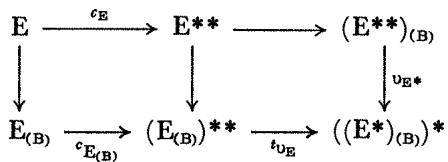
\includegraphics[keepaspectratio]{images/part003_7dd43288.jpg}}

是交换的。

\begin{enumerate}
\def\labelenumi{\arabic{enumi}.}
\setcounter{enumi}{4}
\item
  设 K 为一个域，A 为乘积环 \(K^{N}\) ，a 为 A 的理想 \(K^{(N)}\) ，B 为环 A/a。证明 a 是投射 A-模但不是有限生成的，尽管 \(a_{(B)} = \{0\}\) 。
\item
  设环 A 和 B 如 §1 习题 7 中所定义，令 M 为一个 A-模；证明 M 是有限生成的（相应地，自由的、投射的）当且仅当 \(M \otimes_{A} B\) 是有限生成的（相应地，自由的、投射的）。
\item
  设 \(\rho: A \to B\) 是一个环同态。对每个左 B-模 \(F\) ，定义典范的 B-模同态
\end{enumerate}

\[
\mathbf {F} \rightarrow \tilde {\rho} (\rho_ {*} (\mathbf {F}))
\]

并证明若 E 是一个左 A-模，则复合映射

\[
\begin{array}{r l} & {\tilde {\rho} (\mathbf {E}) \to \tilde {\rho} (\rho_ {*} (\tilde {\rho} (\mathbf {E}))) \to \tilde {\rho} (\mathbf {E})} \\ & {\rho_ {*} (\mathbf {F}) \to \rho_ {*} (\tilde {\rho} (\rho_ {*} (\mathbf {F}))) \to \rho_ {*} (\mathbf {F})} \end{array}
\]

是恒等映射。

\BourbakiExercisesSection

\begin{enumerate}
\def\labelenumi{\arabic{enumi}.}
\item
  设 \((\mathbf{E}_n, f_{nm})\) 是 \(\mathbf{Z}\) -模的逆向系统，其指标集为 \(\mathbf{N}\) ，使得 \(\mathbf{E}_n = \mathbf{Z}\) （对于所有 \(n\) ），并且对于 \(n \leqslant m\) ， \(f_{nm}\) 是映射 \(x \mapsto 3^{m - n}x\) 。对所有 \(n\) ，设 \(u_n\) 为典范映射 \(\mathbf{E}_n \to \mathbf{Z}/2\mathbf{Z}\) 。证明 \((u_n)\) 是由满射线性映射组成的逆向系统，但 \(\lim u_n\) 不是满射。
\item
  设 \((\mathbf{E}_{\alpha}, f_{\beta\alpha})\) 是 A-模的一个正向系统。证明 A-模 \(\lim_{\rightarrow} E_{\alpha}\) 典范同构于直和 \(\bigoplus_{\alpha} E_{\alpha} = F\) 关于子模 N 的商模，N 由形如 \(j_{\beta}(f_{\beta\alpha}(x_{\alpha})) - j_{\alpha}(x_{\alpha})\) 的元素生成（对于每个有序对 \((\alpha, \beta)\) （满足 \(\alpha \leqslant \beta\) ）以及所有 \(x_{\alpha} \in E_{\alpha}\) ），其中诸 \(j_{\alpha}: E_{\alpha} \to F\) 是典范单射。
\item
  设 \((\mathbf{F}_n, f_{mn})\) 为 \(\mathbf{Z}\) -模的正向系统，使得 \(\mathbf{F}_n\) 等于 \(\mathbf{U}_p\) （ \(\S 1\) ，习题 12(d)）对所有 \(n \geqslant 0\) ，并且 \(f_{mn}\) 是自同态 \(x \mapsto p^{m-n}x\) （ \(\mathbf{U}_p\) 的）（对于 \(n \leqslant m\) ）。证明 \(\lim_{\longrightarrow} \mathbf{F}_n = \{0\}\) ，尽管诸 \(f_{mn}\) 是满射。
\item
  设 \((\mathbf{F}_{\alpha}, f_{\beta \alpha})\) 是 A-模的一个正向系统。
\end{enumerate}

\begin{enumerate}
\def\labelenumi{(\alph{enumi})}
\tightlist
\item
  对每个 A-模 E，定义一个典范 Z-模同态
\end{enumerate}

\[
\varepsilon : \varinjlim \operatorname{Hom} _ {\mathbf {A}} (\mathrm{E}, \mathrm{F} _ {\alpha}) \rightarrow \operatorname{Hom} _ {\mathbf {A}} (\mathrm{E}, \varinjlim \mathrm{F} _ {\alpha}).
\]

\begin{enumerate}
\def\labelenumi{(\alph{enumi})}
\setcounter{enumi}{1}
\item
  证明：若 E 是有限生成的，则 \(\varepsilon\) 是单射。给出一个例子，其中 \(\varepsilon\) 不是单射（参见习题 3，取 \(E = \lim F_{\alpha}\) ）。
\item
  证明若 E 是有限生成的且诸 \(f_{\beta\alpha}\) 都是单射，则 \(\varepsilon\) 是满射。给出一个例子，其中 \(E = \lim_{\longrightarrow} F_{\alpha}\) 是自由的，诸 \(f_{\beta\alpha}\) 是单射，并且 \(\varepsilon\) 不是满射。
\item
  证明：如果 \(\mathbf{E}\) 是投射的且有限生成的， \(\varepsilon\) 是双射。
\end{enumerate}

\(^{*}(e)\) 设 A 是一个整环，a 是 A 的一个非有限生成的理想。若 \((a_{\alpha})\) 是包含在 a 中的有限生成理想的族，证明 E = A/a 典范同构于诸 \(F_{\alpha} = A/a_{\alpha}\) 的正向极限，但同态 \(\varepsilon\) 不是满射。*
% semantic-fragments: legacy-input-seam
\relax{}
\BourbakiExercisesSection

\begin{enumerate}
\def\labelenumi{\arabic{enumi}.}
\item
  证明：若 E 是一个含无穷多个元素的域 K 上的向量空间 \(\neq\{0\}\) ，则 E 的生成系所成的集对于序关系 \(\supset\) 不是归纳的（作出 E 的生成系的一个递减序列 \((S_{n})\) ，使得诸 \(S_{n}\) 的交是空的）。
\item
  设 K 为一个域，L 为 K 的子域，I 为一个集合，且 \((x_{i})_{1\leqslant i\leqslant m}\) 为 \(K_{s}^{I}\) 中的一个自由向量族，使得每个 \(x_{i}\) 的坐标都属于 L。设 V 为 \(K_{s}^{I}\) 中由这些 \(x_{i}\) 生成的向量子空间；证明存在 I 的一个含 m 个元素的有限子集 J，使得对 V 的每个向量 \(z=(\zeta_{\alpha})_{\alpha\in\mathbb{I}}\) ，所有 \(\zeta_{\alpha}\) 都属于由 L 与 m 个元素 \(\zeta_{\beta}\) （其中 \(\beta\in J\) ）生成的 K 的子域。（通过将第 5 节的推论 3 应用于空间 \(L_{s}^{I}\) ，证明可化归于存在 m 个指标 \(\beta_{i}\in I\) （ \(1\leqslant i\leqslant m\) ）使得 \(\Pr_{\beta_{i}}(x_{j})=\delta_{ij}\) 的情形。）
\item
  \begin{enumerate}
  \def\labelenumii{(\alph{enumii})}
  \tightlist
  \item
    设 G 是一个群，M 是 G 的一个无限子集。证明：若 \(G'\) 是由 M 生成的 G 的子群，则 \(\text{Card}(G') = \text{Card}(M)\) 。
  \end{enumerate}
\end{enumerate}

\begin{enumerate}
\def\labelenumi{(\alph{enumi})}
\setcounter{enumi}{1}
\item
  设 \(\mathbf{K}\) 为一个域， \(\mathbf{M}\) 为 \(\mathbf{K}\) 的一个无限子集。证明：若 \(\mathbf{K}'\) 是 \(\mathbf{K}\) 的由 \(\mathbf{M}\) 生成的子域，则 \(\operatorname{Card}(\mathbf{K}') = \operatorname{Card}(\mathbf{M})\) 。（考虑子集的两个序列 \((\mathbf{A}_n)_{n \geqslant 0}, (\mathbf{P}_n)_{n \geqslant 0}\) （这些子集属于 \(\mathbf{K}\) ），使得 \(\mathbf{A}_0 = \mathbf{M}\) ， \(\mathbf{P}_n\) 是 \(\mathbf{K}^*\) 的由 \(\mathbf{A}_n \cap \mathbf{K}^*\) 生成的乘法子群，而 \(\mathbf{A}_{n+1}\) 是 \(\mathbf{K}\) 的由 \(\mathbf{P}_n\) 生成的加法子群；然后应用 (a)。）
\item
  设 K 为一个域，I 为一个无限集；证明 \(\operatorname{Card}(\mathbf{K}) \leqslant \dim(\mathbf{K}_{s}^{\mathbf{I}})\) 。（将其归结为 I = N 的情形，并用反证法论证。设 B 为 \(K_{s}^{N}\) 的满足 \(\operatorname{Card}(\mathbf{B}) < \operatorname{Card}(\mathbf{K})\) 的一组基，并设 L 为 K 中由 B 的所有元素的坐标生成的子域；则 \(\operatorname{Card}(\mathbf{L}) < \operatorname{Card}(\mathbf{K})\) 。构造 K 中元素的一个序列 \((\xi_{n})_{n \geqslant 1}\) ，使得对所有 n， \(\xi_{n}\) 不属于 K 中由 L 与诸 \(\xi_{i}\) （其指标 i \textless{} n ）生成的子域；然后应用习题 2，通过考虑点 \(x = (\xi_{n})\) （属于 \(K_{s}^{N}\) ）得出矛盾。）
\item
  由(c)可推出，对任意域K及任意无限集I，
\end{enumerate}

\[
\dim (\mathrm{K} _ {s} ^ {\mathrm{I}}) = (\operatorname{Card} (\mathrm{K})) ^ {\operatorname{Card} (\mathrm{I})}
\]

(``Erdös-Kaplansky 定理'').

4 给出一个无限序列 \((\mathbf{F}_n)\) 的例子，该序列由某个向量空间 \(\mathbf{E}\) 的向量子空间组成，使得 \(\operatorname{codim}\left(\bigcap_{n} \mathbf{F}_n\right) > \sum_{n} \operatorname{codim}(\mathbf{F}_n)\) 。（取 \(\operatorname{codim}(\mathbf{F}_n) = 1\) 对所有 \(n\) 成立，并利用习题 3 \((d)\) 。）

\begin{enumerate}
\def\labelenumi{\arabic{enumi}.}
\setcounter{enumi}{4}
\tightlist
\item
  设 \((\mathbf{H}_{\lambda})_{\lambda \in L}\) 是向量空间 \(\mathbf{E}\) （在域 \(\mathbf{K}\) 上）的一族超平面（经过 0），它构成 \(\mathbf{E}\) 的一个覆盖。
\end{enumerate}

\begin{enumerate}
\def\labelenumi{(\alph{enumi})}
\item
  证明：若 K 有限，则 \(\operatorname{Card}(\mathbf{L}) \geqslant 1 + \operatorname{Card}(\mathbf{K})\) ；若 K 无限，则 \(\operatorname{Card}(\mathbf{L}) \geqslant \aleph_{0} = \operatorname{Card}(\mathbf{N})\) 。（对 r 作归纳证明：若 K 至少有 r 个元素，则 E 不能是 r 个超平面的并。）用例子说明，在没有附加假设的情况下，这些不等式不能改进（当 K 无限时，考虑空间 \(\mathbf{E} = \mathbf{K}_{s}^{(\mathbf{N})}\) ）。
\item
  若 E 是有限维的，证明 \(\operatorname{Card}(\mathbf{L}) \geqslant 1 + \operatorname{Card}(\mathbf{K})\) 。（对 \(\dim(\mathbf{E})\) 作归纳论证。）这一结论在无限维时不再成立；考虑 \(K^{(N)}\)
\end{enumerate}

¶ 6. 设 S 是向量 K-空间 E 的一个非空有限子集，且不包含 0。假设存在一个整数 \(k \geqslant 1\) 具有如下性质：(*) 对所有 \(x \in S\) ，存在 \(S = \{x\}\) 到 \(h\) 个自由子集的一个划分，其中 \(h \leqslant k\) 。

对于这样的划分 \((\mathbf{N}_i)_{1\leqslant i\leqslant h}\) 与每个整数序列 \((r_j)_{1\leqslant j\leqslant m}\) （整数取自 \(\{1,h\}\) ），子空间 \(\mathrm{F}_{r_1r_2\dots r_m}\) （属于 \(\mathbf{E}\) ）按对 \(m\) 的归纳定义如下： \(\mathrm{F}_{r_1}\) 是由 \(\mathrm{N}_{r_1},\mathrm{F}_{r_1\dots r_p}\) 生成的子空间，后者为由 \(\mathrm{F}_{r_1\dots r_{p-1}}\) 与 \(\mathrm{N}_{r_p}\) 的交所生成的子空间。假设：

(**) 对所有 \(x \in S\) 以及每个划分 \((N_i)_{1 \leqslant i \leqslant h}\) （将 \(S = \{x\}\) 分为至多 \(k\) 个自由子集），至少存在一个序列 \((r_j)_{1 \leqslant j \leqslant m}\) ，使得

\[
x \notin \mathrm{F} _ {r _ {1} r _ {2} \dots r _ {m}}.
\]

\begin{enumerate}
\def\labelenumi{(\alph{enumi})}
\item
  设 \(n\) 是整数 \(m \geqslant 1\) （对 \(x \in S\) 的所有可能选取）中的最小者，并设 \((\mathbf{N}_i)_{1 \leqslant i \leqslant h}\) 和 \((r_j)_{1 \leqslant j \leqslant m}\) 满足条件 (*) 和 (**)。证明必然有 \(n = 1\) 。（用反证法论证，假设 \(x \notin F_{r_1 r_2 \ldots r_n}\) 且 \(n > 1\) 。则必有 \(x \in F_{r_n}\) 。为简单起见，记 \(E_p = F_{r_1 r_2 \ldots r_p}\) （ \(1 \leqslant p \leqslant n\) ），并写 \(x = \sum_i \alpha_i y_i\) ，其中 \(\alpha_i \in K\) ， \(y_i \in N_{r_n}\) ；至少有一个 \(y_i\) 不属于 \(E_{n-1}\) ，把它记作 \(y\) ；然后令 \(N = N_{r_n} - \{y\}\) ，令 \(N_i' = N_i\) （ \(1 \leqslant i \leqslant h\) 且 \(i \neq r_n\) ），令 \(N_{r_n}' = N \cup \{x\}\) ，使得 \((\mathbf{N}_i')_{1 \leqslant i \leqslant h}\) 是由自由子集组成的 \(S - \{y\}\) 的一个划分。定义 \(E_0' = E\) ，并对 \(1 \leqslant p \leqslant n\) 把 \(E_p'\) 定义为由 \(E_{p-1}'\) 与 \(N_{r_p}'\) 的交生成的子空间。现在 \(y \notin E_{n-1}\) ；令 \(q\) 为使 \(y \notin E_q\) 的最小整数；证明 \(E_q' \not\subset E_q\) 。令 \(s\) 为使 \(E_s' \not\subset E_s\) 的最小整数；证明 \(r_s = r_n\) ；最后由关系 \(y \in E_s, E_{s-1}' \subset E_{s-1}\) 与 \(E_s' \not\subset E_s\) 推出矛盾。
\item
  由 (a) 推出，在给定假设下，存在 S 到 h 个自由子集的一个划分，其中整数 \(h \leqslant k\) 。
\end{enumerate}

\begin{enumerate}
\def\labelenumi{\arabic{enumi}.}
\setcounter{enumi}{6}
\tightlist
\item
  设 S 是向量 K-空间 E 的一个非空有限子集，且不包含 0。假设存在一个整数 \(k \geqslant 1\) 使得对于每个子集
\end{enumerate}

S 的每个子集 T，有 \(\text{Card}(T) \leqslant k.\text{rg}(T)\) 。证明存在将 S 分为 h 个自由子集的一个划分，其中某个整数 \(h \leqslant k\) 。（证明 S 满足习题 6 的条件（ \(^{**}\) ），对 \(\text{Card}(S)\) 作归纳论证，并在所有子空间 \(F_{r_{1}\ldots r_{m}}\) 中取一个维数尽可能小的子空间；若 G 是这样的子空间，且 j 是使 \(\text{Card}(G \cap N_{j})\) 为最小的指标，则证明

\[
\begin{array}{r l} k. \operatorname{Card} (\mathrm{G} \cap \mathrm{N} _ {j}) & \leqslant \operatorname{Card} (\mathrm{G} \cap (\mathrm{S} - \{x \})) \\ & \leqslant \operatorname{Card} (\mathrm{G} \cap \mathrm{S}) \leqslant k. \operatorname{Card} (\mathrm{G} \cap \mathrm{N} _ {j}).) \end{array}
\]

\begin{enumerate}
\def\labelenumi{\arabic{enumi}.}
\setcounter{enumi}{7}
\item
  设 E 是一个向量空间。证明 E 的每个在 End(E) 中不是 0 的右因子的自同态都是满射的（§ 2，习题 7）。
\item
  设K是一个域。
\end{enumerate}

\begin{enumerate}
\def\labelenumi{(\alph{enumi})}
\item
  在向量空间 \(\mathbf{E} = \mathrm{K}_s^{(\mathbf{Z})}\) 中，设 \((e_n)_{n\in \mathbf{Z}}\) 为典范基；设 \(v\) 为 \(\mathbf{E}\) 的由关系 \(v(e_n) = e_{n + 1}\) （对所有 \(n\in \mathbf{Z}\) ）定义的自同构。若 \(u = 1_{\mathbb{E}} - v\) ，证明 \(u\) 是 \(\mathbf{E}\) 的一个单射自同态，但 \(\dim (\operatorname {Coker}(u)) = 1\) 。
\item
  在向量空间 \(\mathbf{E} = \mathrm{K}_s^{(\mathbb{N})}\) 中，设 \((e_n)_{n\in \mathbb{N}}\) 为典范基；设 \(v\) 为 \(\mathbf{E}\) 的由 \(v(e_0) = e_0\) ， \(v(e_n) = e_{n - 1} + e_n\) （对 \(n\geqslant 1\) ）定义的自同态。证明 \(v\) 是 \(\mathbf{E}\) 的一个自同构，且若 \(u = 1_{\mathbb{E}} - v\) ，则 \(u\) 是 \(\mathbf{E}\) 的满足 \(\dim (\mathrm{Ker}(u)) = 1\) 的一个满射自同态。
\item
  设 I 为一个非空集合。证明向量空间 \(E = K_{s}^{(I)}\) 的每个自同构 u 都可以写成两个自同构之差 u = v - w，除非 K 只有两个元素且 I 仅由一个元素组成。（注意只需证明某个特定的自同构 u 具有所述形式即可；当 K 是两个元素的域时，分别考虑 \(\text{Card}(I) = 2\) 与 \(\text{Card}(I) = 3\) 的情形。）
\end{enumerate}

设 E 是域 K 上的向量空间。证明 E 的每个自同态 u 要么是自同构，要么可以写成 u = v - w，其中 v 和 w 是 E 的自同构。（注意，u 总可以换成 \(s_{1} \circ u \circ s_{2}\) ，其中 \(s_{1}\) 和 \(s_{2}\) 是 E 的两个自同构。区分两种情形，视 \(\dim(\text{Ker}(u)) \leqslant \dim(\text{Coker}(u))\) 还是 \(\dim(\text{Ker}(u)) > \dim(\text{Coker}(u))\) 而定；当 \(\text{rg}(u)\) 有限时，第一种情形总成立。当

\[
\dim (\operatorname{Ker} (u)) \leqslant \dim (\operatorname{Coker} (u)),
\]

它可以简化为以下情形： \(\operatorname{Ker}(u) \cap \operatorname{Im}(u) = \{0\}\) ；若

\[
\dim (\operatorname{Ker} (u)) = \dim (\operatorname{Coker} (u)),
\]

还可以假设 \(\operatorname{Im}(u) + \operatorname{Ker}(u) = \mathbf{E}\) ，然后应用习题 9 (c)。若 \(\dim (\operatorname {Ker}(u)) < \dim (\operatorname {Coker}(u))\) ，则在 \(\mathbf{E}\) 中存在 \(\operatorname {Ker}(u)\) 的一个形如 \(\mathbf{W} \oplus \operatorname{Im}(u)\) 的补子空间，满足 \(\dim (\mathbf{W}) = \dim (\operatorname {Im}(u)) = \dim (\mathbf{E})\) ；应用开头的注记并取 \(s_1(u(\operatorname {Im}(u))) = \operatorname{Im}(u)\) ，并利用习题 9 (a) 和 (c)。当 \(\dim (\operatorname {Ker}(u)) > \dim (\operatorname {Coker}(u))\) 时，可化归于 \(\operatorname{Ker}(u) \subset \operatorname{Im}(u)\) 的情形；这次取 \(s_1(\operatorname{Ker}(u)) = u(\operatorname{Ker}(u))\) ，并利用前面诸情形及习题 9 的结果。）

\begin{enumerate}
\def\labelenumi{\arabic{enumi}.}
\setcounter{enumi}{10}
\tightlist
\item
  设 E、F 是域 K 上的两个向量空间， \(u: E \rightarrow F\) 是一个线性映射。证明对于 F 的每个向量子空间 V，
\end{enumerate}

\[
\dim (u ^ {- 1} (\mathbf {V})) = \dim (\mathbf {V} \cap \operatorname{Im} (u)) + \dim (\operatorname{Ker} (u)).
\]

\begin{enumerate}
\def\labelenumi{\arabic{enumi}.}
\setcounter{enumi}{11}
\tightlist
\item
  设 E、F 为两个向量空间，u、v 为从 E 到 F 的两个线性映射。
\end{enumerate}

\begin{enumerate}
\def\labelenumi{(\alph{enumi})}
\tightlist
\item
  证明以下不等式成立：
\end{enumerate}

\[
\begin{array}{c} \operatorname{rg} (v) \leqslant \operatorname{rg} (u + v) + \operatorname{rg} (u) \\ \operatorname{rg} (u + v) \leqslant \inf (\dim (\mathrm{E}), \dim (\mathrm{F}), \operatorname{rg} (u) + \operatorname{rg} (v)). \end{array}
\]

若E和F是有限维的，证明 \(\operatorname{rg}(u + v)\) 可以取满足不等式的任意整数值

\[
\left| \operatorname{rg} (u) - \operatorname{rg} (v) \right| \leqslant \operatorname{rg} (u + v) \leqslant \inf (\dim (\mathrm{E}), \dim (\mathrm{F}), \operatorname{rg} (u) + \operatorname{rg} (v)).
\]

\begin{enumerate}
\def\labelenumi{(\alph{enumi})}
\setcounter{enumi}{1}
\tightlist
\item
  证明
\end{enumerate}

\[
\dim (\operatorname{Ker} (u + v)) \leqslant \dim (\operatorname{Ker} (u) \cap \operatorname{Ker} (v)) + \dim (\operatorname{Im} (u) \cap \operatorname{Im} (v)).
\]

\begin{enumerate}
\def\labelenumi{(\alph{enumi})}
\setcounter{enumi}{2}
\tightlist
\item
  证明
\end{enumerate}

\[
\dim (\operatorname{Coker} (u + v)) \leqslant \dim (\operatorname{Coker} (u)) + \operatorname{rg} (v).
\]

（若 \(\mathbf{V}\) 是 \(\operatorname{Ker}(v)\) 在 \(\mathbf{E}\) 中的一个补子空间，注意

\[
u (\operatorname{Ker} (v)) \subset \operatorname{Im} (u + v) \quad \text { and } \quad \dim (u (\mathbf {V})) \leqslant \operatorname{rg} (v).)
\]

\begin{enumerate}
\def\labelenumi{\arabic{enumi}.}
\setcounter{enumi}{12}
\tightlist
\item
  设 E、F、G 为三个向量空间，且 \(u: \mathbf{E} \to \mathbf{F}\) , \(v: \mathbf{F} \to \mathbf{G}\) 为两个线性映射。
\end{enumerate}

\begin{enumerate}
\def\labelenumi{(\alph{enumi})}
\tightlist
\item
  证明存在将 E 分解为 \(\operatorname{Ker}(u)\) 与两个子空间 M, N 的直和，使得 \(\operatorname{Ker}(v \circ u) = \mathbf{M} \oplus \operatorname{Ker}(u)\) 和
\end{enumerate}

\[
\operatorname{Im} (v \circ u) = v (u (\mathbf {N})).
\]

\begin{enumerate}
\def\labelenumi{(\alph{enumi})}
\setcounter{enumi}{1}
\item
  \(\dim(\operatorname{Ker}(u)) \leqslant \dim(\operatorname{Ker}(v \circ u)) \leqslant \dim(\operatorname{Ker}(u)) + \dim(\operatorname{Ker}(v))\) ；若 \(\operatorname{Ker}(u)\) 和 \(\operatorname{Ker}(v)\) 是有限维的，证明 \(\dim(\operatorname{Ker}(v \circ u))\) 可以取满足上述不等式的每一个整数值。
\item
  以下等式成立：
\end{enumerate}

\[
\begin{array}{l} \operatorname{rg} (u) = \operatorname{rg} (v \circ u) + \dim (\operatorname{Im} (u) \cap \operatorname{Ker} (v)) \\ \operatorname{rg} (v) = \operatorname{rg} (v \circ u) + \operatorname{codim} _ {\mathbb {F}} (\operatorname{Im} (u) + \operatorname{Ker} (v)). \end{array}
\]

若 F 是有限维的，证明 \(\operatorname{rg}(v \circ u)\) 可以取满足该不等式的任意整数值

\[
\sup (0, \operatorname{rg} (u) + \operatorname{rg} (v) - n) \leqslant \operatorname{rg} (v \circ u) \leqslant \inf (\operatorname{rg} (u), \operatorname{rg} (v)).
\]

\begin{enumerate}
\def\labelenumi{\arabic{enumi}.}
\setcounter{enumi}{13}
\item
  设 E、F、G 为三个向量空间，且 \(u: \mathbf{E} \to \mathbf{F}\) , \(w: \mathbf{E} \to \mathbf{G}\) 两个线性映射。证明若 \(u(0) \subset w(0)\) ，存在一个线性映射 \(v\) ，使得 \(w = v \circ u\) （参见第2节，习题8）。
\item
  设E，F是域K上的两个向量空间， \(u: E \rightarrow F\) 是一个线性映射。
\end{enumerate}

\begin{enumerate}
\def\labelenumi{(\alph{enumi})}
\item
  下列条件等价：（1） \(\operatorname{Ker}(u)\) 是有限维的；（2）存在一个线性映射 \(v\) （由 \(\mathbf{F}\) 到 \(\mathbf{E}\) ），使得 \(v \circ u = 1_{\mathbf{E}} + w\) ，其中 \(w\) 是 \(\mathbf{E}\) 的一个有限秩自同态；（3）对每个向量空间 \(\mathbf{G}\) （在 \(\mathbf{K}\) 上）与每个线性映射 \(f: \mathbf{G} \to \mathbf{E}\) ，关系 \(\operatorname{rg}(u \circ f) < +\infty\) 蕴含 \(\operatorname{rg}(f) < +\infty\) 。
\item
  以下条件等价：（1）Coker(u)是有限维的；（2）存在一个线性映射v：F→E，使得 \(u \circ v = 1_{F} + w\) ，其中w是F的一个有限秩自同态；（3）对于K上的每个向量空间G和每个线性映射 \(g: F \to G\) ，关系 \(\operatorname{rg}(g \circ u) < +\infty\) 蕴含 \(\operatorname{rg}(g) < +\infty\) .
\end{enumerate}

\begin{enumerate}
\def\labelenumi{\arabic{enumi}.}
\setcounter{enumi}{15}
\tightlist
\item
  设 E、F 是 K 上的两个向量空间， \(u: E \to F\) 是一个线性映射。若 \(\operatorname{Ker}(u)\) 和 \(\operatorname{Coker}(u)\) 都是有限维的，则称 u 具有有限指标，且数 \(d(u) = \dim(\operatorname{Ker}(u)) - \dim(\operatorname{Coker}(u))\) 称为 u 的指标。
\end{enumerate}

设G是K上的第三个向量空间， \(v: F \rightarrow G\) 一个线性映射。证明：如果三个线性映射 u, v, \(v \circ u\) 中有两个具有有限指标，则第三个也具有有限指标，且 \(d(v \circ u) = d(u) + d(v)\) （利用习题13(a)）。

\begin{enumerate}
\def\labelenumi{\arabic{enumi}.}
\setcounter{enumi}{16}
\tightlist
\item
  设 E, F, G, H 是 K 上的四个向量空间，且 \(u: E \rightarrow F\) , \(v: F \rightarrow G\) , \(w: G \rightarrow H\) 三个线性映射。证明
\end{enumerate}

\[
\operatorname{rg} (v \circ u) + \operatorname{rg} (w \circ v) \leqslant \operatorname{rg} (v) + \operatorname{rg} (w \circ v \circ u).
\]

\begin{enumerate}
\def\labelenumi{\arabic{enumi}.}
\setcounter{enumi}{17}
\item
  设 E、F 是域 K 上的两个向量空间，u、v 是 E 到 F 的两个线性映射。要使存在 E 的自同构 f 和 F 的自同构 g 使得 \(v = g \circ u \circ f\) ，必要且充分的条件是 \(\operatorname{rg}(u) = \operatorname{rg}(v)\) , \(\dim(\operatorname{Ker}(u)) = \dim(\operatorname{Ker}(v))\) 与 \(\dim(\operatorname{Coker}(u)) = \dim(\operatorname{Coker}(v))\) 。
\item
  设 E 是域 K 上的一个向量空间。
\end{enumerate}

\begin{enumerate}
\def\labelenumi{(\alph{enumi})}
\item
  证明每个映射 \(f\) （由 \(\mathbf{E}\) 到 \(\mathbf{E}\) ）只要与 \(\mathbf{E}\) 的所有自同构可交换，就具有形式 \(x \mapsto \alpha x\) ，其中 \(\alpha \in \mathbf{K}\) （首先证明：对所有 \(x \in \mathbf{E}\) 存在 \(\rho(x) \in \mathbf{K}\) 使得 \(f(x) = \rho(x)x\) ，利用 \(f\) 与 \(\mathbf{E}\) 的每个使 \(x\) 不变的自同构可交换这一事实）。
\item
  设 \(g\) 是 \(\mathbf{E} \times \mathbf{E}\) 到 \(\mathbf{E}\) 的一个映射，使得对每个自同构 \(u\) （属于 \(\mathbf{E}\) ）都有 \(g(u(x), u(y)) = u(g(x, y))\) （对所有 \(x, y\) 属于 \(\mathbf{E}\) ）。证明存在两个元素 \(\alpha, \beta\) （属于 \(\mathbf{K}\) ），使得 \(g(x, y) = \alpha x + \beta y\) 在由线性无关元素组成的有序对 \((x, y)\) （这些元素属于 \(\mathbf{E}\) ）所成的集合上成立；此外，存在一个映射 \(\phi\) （由 \(\mathbf{K} \times \mathbf{K}\) 到 \(\mathbf{K}\) ），使得 \(g(\lambda x, \mu x) = \phi(\lambda, \mu)x\) 对所有 \(x \in \mathbf{E}\) 成立（同样的方法）。若进一步 \(g(u(x), u(y)) = u(g(x, y))\) 对每个自同态 \(u\) （属于 \(\mathbf{E}\) ）成立，则 \(g(x, y) = \alpha x + \beta y\) 对所有 \(x, y\) （属于 \(\mathbf{E}\) ）成立。推广到 \(\mathbf{E}^n\) 到 \(\mathbf{E}\) 的映射。
\end{enumerate}

\begin{enumerate}
\def\labelenumi{\arabic{enumi}.}
\setcounter{enumi}{19}
\tightlist
\item
  设 E 是一个向量空间。
\end{enumerate}

\begin{enumerate}
\def\labelenumi{(\alph{enumi})}
\item
  证明：若 M 和 N 是 E 的两个向量子空间，而 M'、N' 分别是 \(\mathbf{M}\) 和 \(\mathbf{N}\) 在 \(\mathbf{E}^*\) 中的正交，则 \(\mathbf{M} \cap \mathbf{N}\) 的正交是 \(\mathbf{M}' + \mathbf{N}'\) （参见 § 2，习题 9 (a)）。
\item
  若 E 是无限维的，证明存在超平面 \(H'\) （属于 \(E^{*}\) ），使得 E 中与 \(H'\) 正交的子空间化为 0（考虑一个包含对应于 E 的一组基的坐标形式的超平面）。
\item
  证明：若 \(\mathbf{E}\) 是无限维的，则存在子空间的一个无限族 \((\mathbf{V}_i)\) （这些子空间属于 \(\mathbf{E}\) ），使得若 \(\mathbf{V}_i'\) 是 \(\mathbf{E}^*\) 中与 \(\mathbf{V}_i\) 正交的子空间，则 \(\mathbf{E}^*\) 中与 \(\bigcap_{i} \mathbf{V}_i\) 正交的子空间不同于 \(\sum_{i} \mathbf{V}_i'\) 。
\item
  由 (b) 推出，若 E 是无限维的，则存在一个作为直和的分解 \(V' \oplus W'\) （这是 \(E^{*}\) 的一个分解），其中 \(W'\) 是有限维的，使得 E 的子空间 V、W 之和 \(V + W\) （其中 V、W 分别与 \(V'\) 和 \(W'\) 正交）不同于 E。
\item
  为使 E 的一个子空间是有限维的，必要且充分条件是它在 \(E^{*}\) 中的正交具有有限余维数。
\end{enumerate}

\begin{enumerate}
\def\labelenumi{\arabic{enumi}.}
\setcounter{enumi}{20}
\item
  用第 6 节定理 8 的记号，设 \(u\) 表示线性映射 \(x \mapsto (\langle x, x_i^* \rangle)\) （由 \(\mathbf{E}\) 到 \(\mathbf{K}_s^{\mathbf{I}}\) ），并设 \(y_0 = (\eta_i)\) 。 \(\mathbf{K}_d^{(\mathbf{I})}\) 与 \(\mathbf{K}_s^{\mathbf{I}}\) 的对偶的一个子空间在 \(\mathbf{K}_d^{(\mathbf{I})}\) 到其双对偶的典范映射下恒等；然后证明：若 \(\mathbf{N}'\) 是 \(^t u\) 的核，则定理 3（第 5 节）的条件表达了下述事实： \(y_0\) 与 \(\mathbf{N}'\) 和 \(\mathbf{K}_d^{(\mathbf{I})}\) 的交正交。当 \(\mathbf{I}\) 无限且方程组 (21)（第 5 节）具有有限秩时，证明这个交不同于 \(\mathbf{N}'\) （注意 \(\mathbf{N}'\) 这时具有有限余维数）。
\item
  设 E 和 F 是域 K 上的两个向量空间，u 是 E 到 F 的一个线性映射。若 V 是 E 的一个向量子空间，而 \(V'\) 是 V 在 \(E^{*}\) 中的正交，证明 \(u(V)\) 的对偶同构于 \({}^{t}u(F^{*})/(V'\cap{}^{t}u(F^{*}))\) 。若 \(W'\) 是 \(F^{*}\) 的一个使 \({}^{t}u(W')\) 为有限维的子空间，而 W 是 \(W'\) 在 F 中的正交，则 \({}^{t}u(W')\) 同构于空间 \(u(E)/(W\cap u(E))\) 的对偶。
\item
  证明：为使线性映射 \(u\) （由向量空间 \(E\) 到向量空间 \(F\) ）满足 \(\mathrm{rg}(t u) = \mathrm{rg}(u)\) ，必要且充分条件是 \(\mathrm{rg}(u)\) 有限（参见习题 3 (d)）。
\item
  设 E 是交换域 K 上有限维数为 n 的向量空间（ \textgreater{} 1）；证明，除非 n = 2 且 K 是两个元素的域，否则不存在仅依赖于 E 的向量空间结构的同构 \(\phi\) （从 E 到 \(E^{*}\) 上）。（注意，若 \(\phi\) 是这样一个同构，则必然对 E 中的 x、y 以及 E 的每个自同构 u 有 \(\langle x, \phi(y) \rangle = \langle u(x), \phi(u(y)) \rangle\) （集合论，IV，§ 1，第 5 节）。）
\item
  \begin{enumerate}
  \def\labelenumii{(\alph{enumii})}
  \tightlist
  \item
    设 K 为一个域，L 与 M 为两个集合；存在典范包含 \((\mathbf{K}_{s}^{\mathbf{L}})^{(\mathbf{M})}\subset(\mathbf{K}_{s}^{(\mathbf{M})})^{\mathbf{L}}\subset\mathbf{K}_{s}^{\mathbf{L}\times\mathbf{M}}\) 。证明：要使这些向量空间中的两个相等，必要且充分条件是集合 L、M 中有一个是有限的。
  \end{enumerate}
\end{enumerate}

\begin{enumerate}
\def\labelenumi{(\alph{enumi})}
\setcounter{enumi}{1}
\tightlist
\item
  设 \((\mathbf{E}_{\lambda})_{\lambda \in L}\) 是 \(K\) 上的一个右向量空间族，而 \((\mathbf{F}_{\mu})_{\mu \in M}\) 是 \(K\) 上的一个左向量空间族。为使典范映射 (26)（第 7 节）是双射，必要且充分条件是向量空间 \(\prod_{\lambda \in L} \mathbf{E}_{\lambda}, \prod_{\mu \in M} F_{\mu}\) 之一是有限维的（利用 (a)）。
\end{enumerate}

\begin{enumerate}
\def\labelenumi{\arabic{enumi}.}
\setcounter{enumi}{25}
\tightlist
\item
  \begin{enumerate}
  \def\labelenumii{(\alph{enumii})}
  \tightlist
  \item
    设 E、F 是域 K 上的两个左向量空间；为使典范同态 \(E^{*} \otimes_{K} F \to \operatorname{Hom}_{K}(E, F)\) 成为双射，必要且充分条件是空间 E、F 之一是有限维的。
  \end{enumerate}
\end{enumerate}

\begin{enumerate}
\def\labelenumi{(\alph{enumi})}
\setcounter{enumi}{1}
\tightlist
\item
  设 E 是一个右向量空间，F 是域 K 上的一个左向量空间。为使典范同态 \(E \otimes_{K} F \to \operatorname{Hom}_{K}(E^{*}, F)\) 成为双射，必要且充分条件是 E 是有限维的（利用习题 3 (d)）。
\end{enumerate}

\begin{enumerate}
\def\labelenumi{\arabic{enumi}.}
\setcounter{enumi}{26}
\tightlist
\item
  \begin{enumerate}
  \def\labelenumii{(\alph{enumii})}
  \tightlist
  \item
    在命题 16 (i)（第 7 节）的假设下，为使典范同态 (27)（第 7 节）成为双射，必要且充分条件是 E 或 F 为有限维（注意 \(\mathrm{Hom}_{\mathbb{K}}(\mathbf{E},\mathbf{G})\otimes_{\mathbb{L}}\mathbf{F}\) 的一个元素在 (27)（第 7 节）下的像把 E 映到 \(\mathbf{G}\otimes_{\mathbb{L}}\mathbf{F}\) 的一个子空间，它包含在形如 \(\mathbf{G}\otimes_{\mathbb{L}}\mathbf{F}'\) 的子空间中，其中 \(\mathbf{F}'\) 是 \(\mathbf{F}\) 的一个有限维子空间）。
  \end{enumerate}
\end{enumerate}

\begin{enumerate}
\def\labelenumi{(\alph{enumi})}
\setcounter{enumi}{1}
\tightlist
\item
  在命题 16 (ii)（第 7 节）的假设下，为使典范同态 (28)（第 7 节）成为双射，必要且充分条件是有序对 \((\mathbf{E}_1, \mathbf{E}_2), (\mathbf{E}_1, \mathbf{F}_1), (\mathbf{E}_2, \mathbf{F}_2)\) 之一由有限维向量空间组成（利用 (a) 及 § 4 的习题 7）。
\end{enumerate}

\begin{enumerate}
\def\labelenumi{\arabic{enumi}.}
\setcounter{enumi}{27}
\item
  设 \(\rho: \mathbf{K} \to \mathbf{A}\) 是域 \(\mathbf{K}\) 到环 \(\mathbf{A}\) 的一个单射同态，并设 \(\mathbf{E}\) 是 \(\mathbf{K}\) 上的一个左向量空间。为使典范映射 \((\mathbf{E}^*)_{(\mathbf{A})} \to (\mathbf{E}_{(\mathbf{A})})^*\) 是双射，必要且充分条件是 \(\mathbf{E}\) 是有限维的，或者 \(\mathbf{A}\) （视为 \(\mathbf{K}\) 上的右向量空间）是有限维的（利用习题 25 ( \(b\) )）。当这两种情形之一成立时，存在典范双射 \((\mathbf{E}^{**})_{(\mathbf{A})} \to (\mathbf{E}_{(\mathbf{A})})^{**}\) 。
\item
  设 A 是一个整环，K 是它的分式域，E 是一个 A-模，而 T(E) 是它的挠模。
\end{enumerate}

\begin{enumerate}
\def\labelenumi{(\alph{enumi})}
\item
  证明 \(\mathbf{E}\) 上的每个线性形式都在 \(\mathrm{T}(\mathrm{E})\) 上为零，从而对偶空间 \(\mathbf{E}^*\) 和 \((\mathrm{E} / \mathrm{T}(\mathrm{E}))^*\) 典范同构。
\item
  证明典范映射 \((\mathbf{E}^{*})_{(\mathbf{K})}\to (\mathbf{E}_{(\mathbf{K})})^{*}\) 是单射，并且当 \(\mathbf{E}\) 有限生成时它是双射。
\item
  给出一个无挠 A-模 E 的例子，使得 \(E^{*} = \{0\}\) 而 \(E_{(K)} \neq \{0\}\) 。
\end{enumerate}

¶ 30. 设 A 是一个整环，E 和 F 是两个 A-模。证明若 x 是 E 的自由元素而 y 是 F 的自由元素，则 \(x \otimes y \neq 0\) （在 \(E \otimes_{A} F\) 中）。（先将其归结为 E 和 F 都无挠的情形，再归结为 E 和 F 都有限生成的情形，并利用习题 29 (b) 证明存在 \(E \times F\) 到 K 的一个 A-双线性映射 f，使得 \(f(x, y) \neq 0\) 。）

*31. 设 \(\mathbf{K}_0\) 为一个交换域，A 为多项式环 \(\mathrm{K}_0[\mathrm{X},\mathrm{Y}]\) （ \(\mathbf{K}_0\) 上两个未定元的多项式环，它是一个整环），而 E 为 A 的理想 \(\mathrm{AX} + \mathrm{AY}\) 。证明在张量积 \(\mathbf{E} \otimes_{\mathbf{A}} \mathbf{E}\) 中，元素 \(\mathbf{X} \otimes \mathbf{Y} - \mathbf{Y} \otimes \mathbf{X}\) 是 \(\neq 0\) 的，并且 \(\mathrm{XY}(\mathbf{X} \otimes \mathbf{Y} - \mathbf{Y} \otimes \mathbf{X}) = 0\) （考虑 \(\mathbf{E} \times \mathbf{E}\) 到商模 \(\mathbf{A}/\mathbf{E}\) 的 A-双线性映射）。*

\begin{enumerate}
\def\labelenumi{\arabic{enumi}.}
\setcounter{enumi}{31}
\item
  将第 10 节的结果推广到 A 为非交换环且具有左分式域 K 的情形（I，§ 9，习题 15）。（注意，若 \(\xi_{i}\) ( \(1 \leqslant i \leqslant n\) ) 是 K 的元素，则存在 A 中的 \(\alpha \neq 0\) ，使得所有 \(\alpha\xi_{i}\) 都属于 A。）
\item
  设 A 是一个整环。A-模 E 称为可除的，如果对所有 \(x \in E\) 以及 A 中所有 \(\alpha \neq 0\) ，存在 \(y \in E\) 使得 \(\alpha y = x\) 。
\end{enumerate}

\begin{enumerate}
\def\labelenumi{(\alph{enumi})}
\item
  设 E、F 是两个 A-模。证明：若 E 是可除的，则 \(E \otimes_{A} F\) 也是可除的。若 E 是可除的且 F 是无挠的，则 \(\operatorname{Hom}_{\mathbf{A}}(\mathbf{E}, \mathbf{F})\) 是无挠的。若 E 是一个挠 A-模而 F 是可除的，则 \(E \otimes_{A} F = \{0\}\) 。若 E 是一个挠 A-模而 F 是无挠的，则 \(\operatorname{Hom}_{\mathbf{A}}(\mathbf{E}, \mathbf{F}) = \{0\}\) 。
\item
  证明每个内射 A-模（§ 2，习题 11）都是可除的；反之，每个可除的无挠 A-模都是内射的（利用 § 2 习题 11 的判据 (δ)）。
\end{enumerate}

\begin{enumerate}
\def\labelenumi{\arabic{enumi}.}
\setcounter{enumi}{33}
\tightlist
\item
  设 A 是一个整环，P 是一个投射 A-模， \(P'\) 是 P 的一个投射子模，而 \(j: P' \to P\) 是典范单射。证明对每个无挠 A-模 E，同态 \(j \otimes 1: P' \otimes_{A} E \to P \otimes_{A} E\) 是单射（归结为 E 有限生成的情形，并将 E 嵌入一个自由 A-模）。
\end{enumerate}

¶ 35. (a) 设 K 为一个域，E 为一个 (K, K)-双模。假设 E 作为 K 上的左向量空间和右向量空间的维数都等于同一个有限数 n。证明存在 E 的 n 个元素的一个族 \((e_{i})\) ，它对于 E 上的两种向量空间结构中的每一种都是基。（注意，若 \((b_{j})_{1\leq j\leq m}\) 是 E 的一个由 m\textless n 个元素组成的族，它对于 E 上的两种向量空间结构中的每一种都是自由的，而 V 是由 \((b_{j})\) 生成的左向量子空间，W 是右向量子空间，则要么 \(V+W\neq E\) ，要么 \(V\cap CW\) 和 \(W\cap CV\) 都非空；在后一情形，若 \(y\in V\cap CW\) , \(z\in W\cap CV\) , 则 \(y+z\) 与 \(b_{j}\) 一起构成 \(m+1\) 个元素的一个族，它对于 E 上的两种向量空间结构中的每一种都是自由的。）

\begin{enumerate}
\def\labelenumi{(\alph{enumi})}
\setcounter{enumi}{1}
\item
  设 F 是 E 的一个子双模，其在 K 上的两种向量空间结构具有相同的维数 p \textless{} n.～证明存在 E 的元素的一个族 \((e_{i})_{1 \leqslant i \leqslant n}\) ，它对于 E 的每一种向量空间结构都是 E 的一组基，并且使得 \((e_{i})_{1 \leqslant i \leqslant p}\) 是 F 在其两种向量空间结构下的基（方法相同）。
\item
  设 \((b_{j})_{1\leqslant j\leqslant n - 1}\) 是 \(n - 1\) 个元素（属于 \(\mathbf{E}\) ）的一个族，它对于 \(\mathbf{E}\) 上的两种向量空间结构中的每一种都是自由的。设 \(\mathbf{V}\) （相应地，W）是 \((b_{j})\) 在 \(\mathbf{E}\) （视为左（相应地，右）向量空间）中生成的超平面。
\end{enumerate}

证明：若 \(\mathbf{V} \subset \mathbf{W}\) （相应地， \(\mathbf{W} \subset \mathbf{V}\) ），则必然 \(\mathbf{V} = \mathbf{W}\) （注意，若 \(a \notin \mathbf{W}\) ，则 \(\lambda \in \mathbf{K}\) 中使 \(\lambda a \in \mathbf{W}\) 的那些 λ 所成的集是一个左理想）。

设 \(\mathbf{K}_0\) 是一个交换域，而 \(\mathbf{K} = \mathbf{K}_0(\mathbf{X})\) 是 \(\mathbf{K}_0\) 上一个未定元的有理函数域（第四章）。在 K 上定义一个 (K, K)-双模结构如下：乘积 \(t.u\) （一个元素 \(u \in \mathbf{K}\) 与一个左算子 \(t \in \mathbf{K}\) 的乘积）是有理函数 \(t(\mathbf{X})u(\mathbf{X})\) ；乘积 \(u.t\) （ \(u\) 与一个右算子 \(t \in \mathbf{K}\) 的乘积）是有理函数 \(u(\mathbf{X})t(\mathbf{X}^2)\) ；这样在 K 上定义的左（相应地，右）向量 K-空间结构是 1 维的（相应地，2 维的）。由此推出 (K, K)-双模的一些例子，使得这种双模的两种向量空间结构的维数是任意整数。

\begin{enumerate}
\def\labelenumi{(\alph{enumi})}
\setcounter{enumi}{1}
\tightlist
\item
  从 (a) 推出一个 (K, K)-双模 E 的例子，其两个向量空间结构具有相同的维数，并且存在 E 的一个子双模 F，它的两个向量空间结构不具有相同的维数。*
\end{enumerate}

设 E 是一个左向量空间（有限维或无限维均可），而 \(A_{i}\) ( \(1 \leqslant i \leqslant n\) ) 是 E 的向量子空间。假设对点的每个序列 \((a_{i})_{1 \leqslant i \leqslant n}\) （这些点属于 E）使得对所有 i 有 \(a_{i} \in A_{i}\) ，由 \(a_{i}\) 生成的 E 的向量子空间都具有维数 \(\leqslant m\) （m 是一个整数 \(\leqslant n\) ）。证明存在 E 的一个维数为 \(h \leqslant m\) 的子空间 W，它包含 \(h + (n - m)\) 个子空间 \(A_{i}\) 。（对 n 作归纳论证。首先证明（对固定的 n）可以只考虑 m \textless{} n 且对所有 i 有 \(\dim(A_{i}) \leqslant m\) 的情形；还可假设对所有 i 有 \(A_{i} \neq \{0\}\) ，且这些 \(A_{i}\) 并不都是

维数为 1 的。然后（对固定的 \(n\) ）对 \(d = \sum_{i=1}^{m} \dim(A_i)\) 作归纳论证。例如，若 \(\dim(A_n) \geqslant 2\) ，考虑一个 1 维子空间 \(B_n\) （包含于 \(A_n\) ），并将归纳假设应用于 \(A_1, \ldots, A_{n-1}, B_n\) ；由此得出结论：存在一个数 \(k\) 使得 \(1 \leqslant k \leqslant m\) ，以及 E 的一个 \(k\) 维子空间 U，它包含 \(k\) 个 \(A_i\) （例如 \(A_1, \ldots, A_k\) ）；如有必要，把 \(k\) 换成一个整数 \(k'\) （满足 \(1 \leqslant k' \leqslant k\) ），并同时证明可以假设存在向量 \(b_i \in A_i\) （对 \(1 \leqslant i \leqslant k\) ）使得 \(b_1, \ldots, b_k\) 构成 U 的一组基；然后投影到 E 中 U 的一个补子空间上，并利用归纳假设。）

\begin{enumerate}
\def\labelenumi{(\alph{enumi})}
\setcounter{enumi}{1}
\tightlist
\item
  设 K 是一个有限域，E 是 K 上的一个 N 维向量空间。设 \(U_{i}\) ( \(1 \leqslant i \leqslant n\) ) 是 E 的向量子空间，使得对 \([1, n]\) 的每个子集 H，诸 \(U_{i}\) （其中 \(i \in H\) ）的交具有维数 \(\leqslant N - \text{Card}(H)\) 。证明这些 \(U_{i}\) 的并不能等于 E（利用对偶性并借助 (a) 论证）。
\end{enumerate}

\begin{enumerate}
\def\labelenumi{\arabic{enumi}.}
\setcounter{enumi}{37}
\item
  设 K 为特征 0 的交换域，E 为 K 上的有限维向量空间。设 \(p_{1}, \ldots, p_{m}\) 为 E 到 E 的向量子空间上的投影算子，使得 \(1_{E} = p_{1} + p_{2} + \cdots + p_{m}\) 。证明 E 是这些 \(p_i(\mathbf{E})\) 的直和，并且这些 \(p_i\) 两两可交换（取两边的迹）。
\item
  设 K 为一个域，L 为 K 的子域，且 \((\mathrm{K}_{\alpha})_{\alpha\in I}\) 为 K 的子域的一个左有向族，使得 \(L=\bigcap_{\alpha\in I}K_{\alpha}\) 。设 E 为 K 上的向量空间，且 \((a_{i})_{1\leqslant i\leqslant m}\) 为 E 的元素的一个有限族；证明若该族 \((a_{i})\) 在 L 上是自由的，则存在一个指标 \(\alpha\) 使得 \((a_{i})\) 在 \(K_{\alpha}\) 上是自由的。（对 m-r 作归纳论证，其中 r 是族 \((a_{i})\) 在 K 上的秩。）
\end{enumerate}

\BourbakiExercisesSection

\begin{enumerate}
\def\labelenumi{\arabic{enumi}.}
\tightlist
\item
  设 K 为一个域， \(K'\) 为 K 的一个子域，而 V 是 K 上的一个非零右向量空间。
\end{enumerate}

\begin{enumerate}
\def\labelenumi{(\alph{enumi})}
\item
  设 \(\mathbf{V}'\) 是一个 \(\mathbf{K}'\) -结构（在 \(\mathbf{V}\) 上）。证明 \(\mathbf{K}'\) 等于由下述 \(\mu \in \mathbf{K}\) 组成的集：对所有 \(x \in \mathbf{V}'\) , \(x\mu \in \mathbf{V}'\) 。
\item
  设 \(\Gamma'\) 为 K 的保持 K' 的元素不变的自同构群。证明：若不存在 K 的不属于 K' 且在所有自同构 \(\sigma \in \Gamma'\) 下不变的元素，则不存在 V 的不属于 V' 且在 V 的每个保持 V' 的所有元素不变的双射双态（相对于 K 的一个自同构）下不变的元素。
\item
  反之，设 E 为 V 的一个子集，G 为保持 E 的所有元素不变的 V 的双射双态群；对所有 \(u \in G\) ，设 \(\sigma_{u}\) 为 K 的相应自同构，并令 \(\Gamma\) 为 K 的自同构群，即 G 在同态 \(u \mapsto \sigma_{u}\) 下的像。假设 G 不包含 V 的不同于恒等自同构的自同构，并且不存在 V 的不属于 E 且在所有双态 \(u \in G\) 下不变的元素。证明：若 \(K'\) 是 K 的在所有自同构 \(\sigma \in \Gamma\) 下不变的元素所成的子域，则 E 是 V 上的一个 \(K'\) -结构。（首先证明 E 是 V 的一个加法子群且包含 V 的一组基；令 \(K''\) 为由下述元素 \(\mu \in K\) 组成的集：关系 \(x \in E\) 蕴含 \(x\mu \in E\) 。证明 \(K''\) 的元素在所有 \(\sigma \in \Gamma\) 下不变，并且 \(K''\) 是 K 的一个子域；由此推出 E 是 V 上的一个 \(K''\) -结构。）
\end{enumerate}

\begin{enumerate}
\def\labelenumi{\arabic{enumi}.}
\setcounter{enumi}{1}
\tightlist
\item
  设 K 为一个域， \(K'\) 为 K 的一个子域，V 是 K 上的一个右向量空间， \(V'\) 是 V 上的一个 \(K'\) -结构，而 \(R'\) 是对偶 \(V'*\) 在 V 的对偶 \(V*\) 中的典范像（第 4 节）。为使 \(R'\) 是 \(V*\) 的一个生成系，必要且充分条件是 V 是有限维的，或者 K 是一个有限维的右向量 \(K'\) -空间（利用 § 7 的习题 25）。
\end{enumerate}

¶ 3. 设 K 是一个域，L 是 K 的一个子域，令 \(K_{L}\) 表示把 K 视为 L 上的左向量空间而得到的域； \(E = \text{End}_{L}(K_{L})\) 典范地具有一个 (K, K)-双模结构。对偶 \((K_{L})^{*}\) 包含在 E 中，并且是 E 的一个 (K, L)-子双模。当 L 包含在 K 的中心内时，E 上的两个 L-向量空间结构——分别把 E 的两个 K-向量空间结构的标量域限制到 L 而得到——是相同的。

此后假设 \(\mathbf{L}\) 包含于 \(\mathbf{K}\) 的中心，且 \(\mathbf{K}_{\mathbf{L}}\) 的维数有限并等于 \(n\) 。

\begin{enumerate}
\def\labelenumi{(\alph{enumi})}
\item
  证明 \((\mathrm{K}_{\mathrm{L}})^{*}\) 在其 K 上的左向量空间结构下是 1 维的（用两种方式计算 \((\mathrm{K}_{\mathrm{L}})^{*}\) 在 L 上的维数）。
\item
  证明 \(\mathbf{E}\) 是一个 \(n\) 维左向量空间（在 \(\mathbf{K}\) 上）（同样的方法）。
\item
  设 F 是 K 上的一个有限维左向量空间，而 \(F_{[L]}\) 是 L 上的相应向量空间。若 \(u_{0} \neq 0\) 是 \(K_{L}\) 上的一个线性形式，证明映射 \(x' \mapsto u_{0} \circ x'\) （由 F 的对偶 \(F^{*}\) （把 F 视为 L 上的向量空间）映到对偶 \((\mathrm{F}_{[\mathrm{L}]})^{*}\) （即 \(F_{[L]}\) 的对偶）上）是双射的（利用 (a)）。
\end{enumerate}

¶ 4. 设 K 是其中心 Z 上有限秩的域，L 是 K 的包含 Z 的子域。

\begin{enumerate}
\def\labelenumi{(\alph{enumi})}
\item
  证明K关于L的左、右向量空间结构具有相同的维数。
\item
  证明习题 3 的性质 (a)、(b)、(c) 在这种情形也成立（若 \(u_0\) 是一个线性形式 \(\neq 0\) （在 \(\mathbf{L}_{\mathbf{Z}}\) 上），而 \(v_0\) 是一个线性形式 \(\neq 0\) （在 \(\mathbf{K}_{\mathbf{L}}\) 上），注意 \(\xi. (u_0 \circ v_0) = u_0 \circ (\xi v_0)\) （对 \(\xi \in \mathbf{K}\) ），并且 \(\xi. (u_0 \circ v_0)\) 遍历对偶 \((\mathbf{K}_{\mathbf{Z}})^*\) （当 \(\xi\) 遍历 \(\mathbf{K}\) 时），并利用习题 3 (c)）。
\end{enumerate}

\begin{enumerate}
\def\labelenumi{\arabic{enumi}.}
\setcounter{enumi}{4}
\tightlist
\item
  设 \(K_{0}\) 是域 K 的一个子域，使得 K 作为 \(K_{0}\) 上的右向量空间具有维数 2。设 E 是 K 上的一个左向量空间。
\end{enumerate}

\begin{enumerate}
\def\labelenumi{(\alph{enumi})}
\item
  设 \(E_{0}\) 是 E 的一个子集，它是 \(K_{0}\) 上的向量空间，并设 V 是 \(E_{0}\) 的最大向量子 K-空间；若 \(W_{0}\) 是一个向量子 \(K_{0}\) -空间（属于 \(E_{0}\) ，与 V 互补），证明由 \(W_{0}\) 生成的 E 的向量子 K-空间 W 满足 \(V \cap W = \{0\}\) （注意，若元素 \(\mu \in K\) 不属于 \(K_{0}\) ，则关系 \(\mu x \in E_{0}\) （对某个 \(x \in E_{0}\) ）蕴含 \(x \in V\) ）。
\item
  设 \(E_{0}^{\prime}\) 是 E 的另一个向量子 \(K_{0}\) -空间，而 \(V^{\prime}\) 是 \(E_{0}^{\prime}\) 的最大向量子 K-空间。为使存在 E 的一个把 \(E_{0}\) 映到 \(E_{0}^{\prime}\) 的 K-自同构，必要且充分条件是 V 和 \(V^{\prime}\) 关于 K 具有相同的维数，V 在 \(E_{0}\) 中与 \(V^{\prime}\) 在 \(E_{0}^{\prime}\) 中的余维数（关于 \(K_{0}\) ）相等，并且 \(E_{0}\) 与 \(E_{0}^{\prime}\) 在 E 中的余维数（关于 \(K_{0}\) ）相等（利用 (a)）。
\end{enumerate}

\BourbakiExercisesSection

*1. 在仿射空间 \(\mathbf{E}\) （在域 \(\mathbf{K}\) 上）中，四元组 \((a, b, c, d)\) （ \(\mathbf{E}\) 的点的四元组）称为平行四边形，如果 \(b - a = c - d\) ，这时 \((a, d, c, b)\) 也是一个平行四边形。证明若 \(\mathbf{K}\) 的特征 \(\neq 2\) ，则有序对 \((a, c)\) 和 \((b, d)\) 的中点相等；当 \(\mathbf{K}\) 的特征为 \(2?_{*}\) 。

*2. 设 E 是特征 \(\neq 2\) 的域上的一个仿射空间，而 \(a, b, c, d\) 是 E 的任意四个点。证明若 \(x, y, z, t\) 分别是有序对 \((a, b), (b, c), (c, d), (d, a)\) 的中点，则四元组 \((x, y, z, t)\) 是一个平行四边形（习题 1）。*

*3. 设 K 是特征 \(\neq 2\) 的交换域，E 是 K 上的一个仿射平面，而 \(a, b, c, d\) 是 E 的四个点，其中任意三点都不共线。设 \(\mathbf{D}_{xy}\) 表示过 E 的两个不同点 \(x, y\) 的直线。假设直线 \(\mathbf{D}_{ab}\) 和 \(\mathbf{D}_{cd}\) 有一个公共点 \(e\) ，且 \(\mathbf{D}_{ad}\) 和 \(\mathbf{D}_{bc}\) 有一个公共点 \(f\) 。证明三个有序对 \((a, c), (b, d), (e, f)\) 的中点位于同一条直线上。当 \(\mathbf{D}_{ab}\) 和 \(\mathbf{D}_{cd}\) 平行或 \(\mathbf{D}_{ad}\) 和 \(\mathbf{D}_{bc}\) 平行时，这一性质变成什么？考虑 K 是 3 个元素的域的情形。*

*4. 设 K 是特征异于 2 和 3 的域，E 是 K 上的一个仿射空间， \(a, b, c\) 是 E 的不在同一条直线上的三个点，而 \(a', b', c'\) 分别是有序对 \((b, c)\) , \((c, a)\) 和 \((a, b)\) 的中点。证明（用习题 3 的记号）直线 \(\mathbf{D}_{aa'}\) , \(\mathbf{D}_{bb'}\) 和 \(\mathbf{D}_{cc'}\) 都过三个点 \(a, b, c\) 的重心。当 K 的特征为 2 或特征为 3 时，这一性质变成什么？推广到 \(n\) 个仿射无关点的系统的情形。*

\begin{enumerate}
\def\labelenumi{\arabic{enumi}.}
\setcounter{enumi}{4}
\item
  设 E 是域 K 上的一个仿射空间，且 K 至少含三个元素。为使 E 的非空子集 V 是一个线性簇，必要且充分条件是：对 V 中每对 \((x,y)\) 不同的点 x 和 y，过 x 和 y 的直线 \(D_{xy}\) 整个包含在 V 中。若 K 恰有两个元素，则为使 V 是一个线性簇，必要且充分条件是 V 的任意三点的重心属于 V。
\item
  \begin{enumerate}
  \def\labelenumii{(\alph{enumii})}
  \tightlist
  \item
    设 E 是域 K 上的一个 \(\geqslant2\) 维仿射空间。为使 E 到自身的仿射映射 u 把 E 的每条直线变为平行直线，必要且充分条件是：与 u 相伴的线性映射 v 是一个位似 \(t\mapsto\gamma t\) （比例 \(\gamma\neq0\) 属于 K 的中心）。若 \(\gamma=1\) ，u 是一个平移；证明若 \(\gamma\neq1\) ，存在且仅存在一个点 \(a\in E\) 使得 \(u(a)=a\) 。若取 a 作为 E 的原点，则 u 在 E 上由此确定的向量空间结构下等同于一个中心位似；u 称为仿射空间 E 的以 a 为中心、以 \(\gamma\) 为比例的中心位似。
  \end{enumerate}
\end{enumerate}

\begin{enumerate}
\def\labelenumi{(\alph{enumi})}
\setcounter{enumi}{1}
\item
  设 \(u_1, u_2\) 是 \(\mathbf{E}\) 到 \(\mathbf{E}\) 的两个仿射映射，其中每一个要么是平移，要么是中心位似。证明 \(u_1 \circ u_2\) 是 \(\mathbf{E}\) 的一个平移或一个中心位似；若 \(u_1, u_2\) 和 \(u_1 \circ u_2\) 这三个都是中心位似，证明它们的中心位于同一条直线上。当 \(u_1\) 和 \(u_2\) 是中心位似而 \(u_1 \circ u_2\) 是平移时，能说些什么？
\item
  证明平移集与中心位似之集构成仿射群的一个正规子群 H，并且 H/T 同构于 K 的中心的乘法群；证明 H 仅当 H = T 时才可能是交换的，换言之，仅当 K 的中心恰含两个元素时。
\end{enumerate}

¶ 7. 设 E（相应地 E'）是域 K（至少含 3 个元素）上的一个有限维 \(n \geqslant 2\) 仿射空间（相应地，域 K' 上的仿射空间），并设 u 是 E 到 E' 的一个单射映射，它把 E 中同一条直线上任意三个点映到同一条直线上的三个点，并且使得由 \(u(E)\) 在 E' 中生成的仿射线性簇等于 E'。

\begin{enumerate}
\def\labelenumi{(\alph{enumi})}
\item
  证明 \(u\) 把 \(E\) 的每个仿射无关点系统映为一个仿射无关点系统（利用习题 5）。
\item
  设 \(D_{1}, D_{2}\) 是 E 中两条平行直线，而 \(D_{1}^{\prime}, D_{2}^{\prime}\) 是 \(E^{\prime}\) 中分别包含 \(u(\mathbf{D}_{1})\) 和 \(u(\mathbf{D}_{2})\) 的直线。证明 \(D_{1}^{\prime}\) 和 \(D_{2}^{\prime}\) 位于同一平面内；若进一步 u 是满射，证明 \(D_{1}^{\prime}\) 和 \(D_{2}^{\prime}\) 平行（在相反情形，证明 E 中会有 3 个不在同一直线上的点，它们在 u 下的像在同一直线上）（参见习题 17）。
\item
  此后假设：若 \(D_{1}\) 和 \(D_{2}\) 是 E 中的平行直线，则 \(E'\) 中分别包含 \(u(\mathbf{D}_{1})\) 和 \(u(\mathbf{D}_{2})\) 的直线是平行的。证明若取 E 中的原点 a 及原点 \(a' = u(a)\) （在 \(E'\) 中），则存在一个同构 \(\sigma\) （把 K 映到一个子域 \(K_{1}\) （属于 \(K'\) ）上），使得若把 E 视为 K 上的向量空间，且把 \(E'\) 作为 \(K_{1}, u\) 上的向量空间，则 u 是一个单射半线性映射（相对于 \(\sigma\) ，由 E 到 \(E'\) ）（§ 1，第 13 节）。（先考虑 n = 2 的情形；给定 E 的一个基 \((e_{1}, e_{2})\) ，证明对 K 的任意两个元素 \(\alpha, \beta\) ，点 \((\alpha + \beta)e_{1}\) 和 \((\alpha\beta)e_{1}\) （属于 E）可以从点 0、 \(e_{1}, e_{2}, \alpha e_{1}, \beta e_{1}\) 出发，通过作给定直线的平行线及给定直线的交点而构造出来；由此推出 \(u(\lambda e_{1}) = \lambda^{\sigma}u(e_{1})\) ，其中 \(\sigma\) 是 K 到 \(K'\) 的一个子域上的同构，然后证明也有 \(u(\lambda e_{2}) = \lambda^{\sigma}u(e_{2})\) （通过考虑连接点 \(\lambda e_{1}\) 和 \(\lambda e_{2}\) 的直线）。最后由此过渡到 n 为任意的情形，对 n 作归纳论证。）若 u 是双射，证明 \(K_{1} = K'\) 。
\item
  把 (c) 的结果推广到 K 是含 2 个元素的域的情形，同时假设 u 也把 E 的每个仿射无关点系统映为 E' 的仿射无关点系统。
\end{enumerate}

\begin{enumerate}
\def\labelenumi{\arabic{enumi}.}
\setcounter{enumi}{7}
\tightlist
\item
  设 E 是域 K 上的左仿射空间，T 为其平移空间。
\end{enumerate}

\begin{enumerate}
\def\labelenumi{(\alph{enumi})}
\tightlist
\item
  为使映射 \(f\) （由 \(\mathbf{E}\) 到一个左向量空间 \(\mathbf{L}\) （在 \(\mathbf{K}\) 上））是仿射的，必要且充分条件是
\end{enumerate}

\[
\begin{array}{r l} f (\mathbf {t} + x) - f (x) & = f (\mathbf {t} + y) - f (y) \\ f (\lambda \mathbf {t} + x) - f (x) & = \lambda f (\mathbf {t} + x) - f (x)) \end{array}
\]

对所有 \(\lambda\in\mathbf{K},\mathbf{t}\in\mathbf{T},x,y\) （在 E 中）。设 \(x\mapsto[x]\) 是 E 到由 E 的元素的形式线性组合所成的向量空间 \(\mathrm{K}_{s}^{(\mathbb{E})}\) 中的典范单射，并设 N 是 \(\mathrm{K}_{s}^{(\mathbb{E})}\) 的由元素

\[
[ \mathbf {t} + x ] - [ x ] - [ \mathbf {t} + y ] + [ y ]
\]

\[
[ \lambda \mathbf {t} + x ] - [ x ] - \lambda [ \mathbf {t} + x ] + \lambda [ x ]
\]

对 \(\lambda \in \mathbf{K}\) , \(\mathbf{t} \in \mathbf{T}\) , \(x, y\) （在 \(\mathbf{E}\) 中）；最后，令 \(\mathbf{V}\) 为 \(\mathbf{K}_s^{(\mathbf{E})}\) 模 \(\mathbf{N}\) 的商空间，并令 \(\phi\) 为 \(\mathbf{E}\) 到 \(\mathbf{V}\) 的映射，它把每个 \(x \in \mathbf{E}\) 对应到 \([x]\) 模 \(\mathbf{N}\) 的类。则 \(\phi\) 是一个仿射映射，并且对每个仿射映射 \(f\) （由 \(\mathbf{E}\) 到一个左向量空间 \(\mathbf{L}\) （在 \(\mathbf{K}\) 上）），存在且仅存在一个线性映射 \(g\) （由 \(\mathbf{V}\) 到 \(\mathbf{L}\) ）使得 \(f = g \circ \phi\) 。

\begin{enumerate}
\def\labelenumi{(\alph{enumi})}
\setcounter{enumi}{1}
\tightlist
\item
  设 \(\phi_0: \mathbf{T} \to \mathbf{V}\) 是与 \(\phi\) 相伴的线性映射，它使得 \(\phi(\mathbf{t} + x) - \phi(x) = \phi_0(\mathbf{t})\) 。证明 \(\phi\) （从而 \(\phi_0\) 也是）是单射（考虑映射 \(x \mapsto x - a\) （由 \(\mathbf{E}\) 到 \(\mathbf{T}\) ，对某个 \(a \in \mathbf{E}\) ））；对每个族 \((\lambda_t)_{t \in I}\) （ \(\mathbf{K}\) 的元素，具有有限支撑）与每个族 \((x_t)_{t \in I}\) （ \(\mathbf{E}\) 的元素），
\end{enumerate}

\[
\sum_ {i} \lambda_ {i} \phi (x _ {i}) = \phi_ {0} \left(\sum_ {i} \lambda_ {i} x _ {i}\right) \quad \text { if } \quad \sum_ {i} \lambda_ {i} = 0
\]

\[
\sum_ {i} \lambda_ {i} \phi (x _ {i}) = \mu \phi_ {0} \left(\sum_ {i} \mu^ {- 1} \lambda_ {i} x _ {i}\right) \quad \text { if } \quad \sum_ {i} \lambda_ {i} = \mu \neq 0.
\]

由此推出 \(\phi_{0}(T)\) 是 V 中过 0 的一个超平面，而 \(\phi(E)\) 是与 \(\phi_{0}(T)\) 平行的一个超平面。

\begin{enumerate}
\def\labelenumi{\arabic{enumi}.}
\setcounter{enumi}{8}
\tightlist
\item
  设 \(\mathbf{K}\) 是一个含 \(q\) 个元素的有限域，而 \(\mathbf{V}\) 是一个 \(n\) 维向量空间（在 \(\mathbf{K}\) 上）。
\end{enumerate}

\begin{enumerate}
\def\labelenumi{(\alph{enumi})}
\tightlist
\item
  证明序列 \((x_{1}, x_{2}, \ldots, x_{m})\) （ \(m \leqslant n\) 个 \(\mathbf{V}\) 的向量，构成自由系统）所成的集的基数等于
\end{enumerate}

\[
(q ^ {n} - 1) (q ^ {n} - q) \dots (q ^ {n} - q ^ {m - 1})
\]

（对 \(n\) 作归纳论证）。

\begin{enumerate}
\def\labelenumi{(\alph{enumi})}
\setcounter{enumi}{1}
\tightlist
\item
  由 (a) 推出，\(m\) 维线性簇（在一个 \(n\) 维射影空间中，空间在域 \(K\) 上）所成的集的基数等于
\end{enumerate}

\[
\frac {(q ^ {n + 1} - 1) (q ^ {n + 1} - q) \dots (q ^ {n + 1} - q ^ {m})}{(q ^ {m + 1} - 1) (q ^ {m + 1} - q) \dots (q ^ {m + 1} - q ^ {m})}.
\]

\begin{enumerate}
\def\labelenumi{\arabic{enumi}.}
\setcounter{enumi}{9}
\item
  在一个 \(n\) 维射影空间 \(\mathbf{P}(\mathbf{V})\) （在域 \(\mathbf{K}\) 上）中，射影基是一个集合 \(\mathbf{S}\) （由 \(n + 2\) 个点组成），其中任意两点都构成一个射影自由系。若 \(\mathbf{S} = (a_i)_{0 \leqslant i \leqslant n + 1}\) 和 \(\mathbf{S}' = (a_i')_{0 \leqslant i \leqslant n + 1}\) 是 \(\mathbf{P}(\mathbf{V})\) 的任意两个射影基，证明存在一个变换 \(f \in \mathbf{PGL}(\mathbf{V})\) 使得 \(f(a_i) = a_i'\) （对 \(0 \leqslant i \leqslant n + 1\) ）。为使这个变换唯一，必要且充分条件是 \(\mathbf{K}\) 可交换。（把它归结为 \(a_i' = a_i\) （对所有 \(i\) ）成立的情形，并注意总可以写成（用第 6 节的记号） \(a_i = \pi(b_i)\) ，其中 \((b_i)_{1 \leqslant i \leqslant n + 1}\) 是 \(\mathbf{V}\) 的一个基，而 \(b_0 = b_1 + b_2 + \cdots + b_{n+1}\) 。） *给出一个例子，其中 \(\mathbf{K}\) 是四元数域，并且存在点的一个无限集 \(\mathbf{T}\) （属于 \(\mathbf{P}(\mathbf{V})\) ），其中任意 \(n + 1\) 个点都构成射影自由系，又存在一个变换 \(f \in \mathbf{PGL}(\mathbf{V})\) ，它不同于恒等变换，且保持 \(\mathbf{T}\) 的所有点不变。*
\item
  设 V 是域 K 上的一个二维向量空间，而 a, b, c, d 是射影直线 \(\mathbf{P}(\mathbf{V})\) 上的四个不同点。四元组 \((a, b, c, d)\) 的交比（记作 \(\begin{bmatrix} a & b \\ d & c \end{bmatrix}\) ）是使下述条件成立的元素 \(\xi \in \mathbf{K}\) 所成的集：存在两个向量 \(u, v\) （在 \(\mathbf{V}\) 中），对它们（用第 6 节的记号）有 \(a = \pi(u)\) , \(b = \pi(v)\) , \(c = \pi(u + v)\) , \(d = \pi(u + \xi v)\) 。这个定义立即推广到具有射影直线结构的集合（第 11 节）的任意四个不同点的四元组。
\end{enumerate}

\begin{enumerate}
\def\labelenumi{(\alph{enumi})}
\item
  证明 \(\begin{bmatrix} a & b \\ d & c \end{bmatrix}\) 是一个元素 \(\neq 1\) （属于乘法群 \(\mathbf{K}^*\) ）的共轭元素的集；反之，当 \(a, b, c\) 是 \(\mathbf{P}(V)\) 的不同点而 \(\rho\) 是一个元素 \(\neq 1\) （属于 \(\mathbf{K}^*\) ）的共轭元素的集时，存在一个点 \(d \in \mathbf{P}(V)\) 使得 \(\begin{bmatrix} a & b \\ d & c \end{bmatrix} = \rho\) 。为使 \(d\) 唯一，必要且充分条件是 \(\rho\) 由单个点组成。
\item
  证明
\end{enumerate}

\[
\left[ \begin{array}{c c} a & b \\ c & d \end{array} \right] = \left[ \begin{array}{c c} b & a \\ d & c \end{array} \right] = \left[ \begin{array}{c c} a & b \\ d & c \end{array} \right] ^ {- 1}
\]

和

\[
\left[ \begin{array}{c c} d & a \\ c & b \end{array} \right] = 1 - \left[ \begin{array}{c c} a & b \\ d & c \end{array} \right]
\]

（用 \(\rho^{-1}\) （相应地， \(1 - \rho\) ）记共轭元素的集 \(\lambda \xi^{-1} \lambda^{-1} = (\lambda \xi \lambda^{-1})^{-1}\) （相应地， \(1 - \lambda \xi \lambda^{-1} = \lambda (1 - \xi) \lambda^{-1}\) ），其中 \(\xi\) 是 \(\rho\) 的一个元素）。

\begin{enumerate}
\def\labelenumi{(\alph{enumi})}
\setcounter{enumi}{2}
\tightlist
\item
  设 \((a, b, c, d)\) , \((a', b', c', d')\) 是 \(\mathbf{P}(\mathbf{V})\) 的两组由不同点组成的四元组。为使存在 V 到自身的一个双射半线性映射，使得在过渡到商时得到的 \(\mathbf{P}(\mathbf{V})\) 到自身的双射映射 f 满足条件 \(f(a) = a'\) , \(f(b) = b'\) , \(f(c) = c'\) , \(f(d) = d'\) ，必要且充分条件是存在 K 的一个自同构 \(\sigma\) 使得
\end{enumerate}

\[
\left[ \begin{array}{c c} a ^ {\prime} & b ^ {\prime} \\ d ^ {\prime} & c ^ {\prime} \end{array} \right] = \left[ \begin{array}{c c} a & b \\ d & c \end{array} \right] ^ {\sigma}.
\]

为使存在射影群 PGL(V) 的一个变换 f 满足上述条件，必要且充分条件是

\[
\left[ \begin{array}{c c} a ^ {\prime} & b ^ {\prime} \\ d ^ {\prime} & c ^ {\prime} \end{array} \right] = \left[ \begin{array}{c c} a & b \\ d & c \end{array} \right].
\]

\begin{enumerate}
\def\labelenumi{\arabic{enumi}.}
\setcounter{enumi}{11}
\tightlist
\item
  设 \(\mathbf{P}(\mathbf{V})\) 是一个有限维数 \(n\) 的（左）射影空间（在域 \(\mathbf{K}\) 上）。证明在 \(\mathbf{P}(\mathbf{V})\) 的射影超平面所成的集上存在一个 \(n\) 维（右）射影空间结构（在 \(\mathbf{K}\) 上），它典范同构于 \(\mathbf{P}(\mathbf{V}^*)\) 的结构（ \(\mathbf{V}^*\) 是 \(\mathbf{V}\) 的对偶）。若 \(\mathbf{M}\) 是维数为 \(r < n\) 的一个线性簇（在 \(\mathbf{P}(\mathbf{V})\) 中），推出一个 \((n - r - 1)\) 维射影空间结构（在包含 \(\mathbf{M}\) 的射影超平面所成的集上）。特别地，若 \(\mathbf{M}\) 的维数为 \(n - 2\) ，可以定义交比 \(\begin{bmatrix} \mathrm{H}_1 & \mathrm{H}_2 \\ \mathrm{H}_4 & \mathrm{H}_3 \end{bmatrix}\) —— 包含 M 的不同超平面的四元组 \((\mathrm{H}_1, \mathrm{H}_2, \mathrm{H}_3, \mathrm{H}_4)\) 的交比。证明若 \(\mathbf{D} \subset \mathbf{P}(\mathbf{V})\) 是一条与 M 不相交的直线，而 \(a_i\) 是 D 与 \(\mathrm{H}_i\) 的交点 ( \(1 \leqslant i \leqslant 4\) )，则
\end{enumerate}

\[
\left[ \begin{array}{c c} a _ {1} & a _ {2} \\ a _ {4} & a _ {3} \end{array} \right] = \left[ \begin{array}{c c} \mathrm{H} _ {1} & \mathrm{H} _ {2} \\ \mathrm{H} _ {4} & \mathrm{H} _ {3} \end{array} \right].
\]

*13. 在射影平面 \(\mathbf{P}(\mathbf{V})\) （在域 \(\mathbf{K}\) 上，特征 \(\neq 2\) ）中，设 \(a, b, c, d\) 是构成一个射影基的四个点（习题 10）；记 \(\mathbf{D}_{xy}\) 为过两个不同点 \(x, y\) （属于 \(\mathbf{P}(\mathbf{V})\) ）的直线，设 \(e, f, g\) 分别是直线 \(\mathbf{D}_{ab}\) 与 \(\mathbf{D}_{cd}\) 、 \(\mathbf{D}_{ac}\) 与 \(\mathbf{D}_{bd}\) 、 \(\mathbf{D}_{ad}\) 与 \(\mathbf{D}_{bc}\) 的交点；令 \(h\) 为 \(\mathbf{D}_{bc}\) 与 \(\mathbf{D}_{ef}\) 的交点；证明 \(\begin{bmatrix} b & c \\ h & g \end{bmatrix} = \{-1\}\) （“完全四边形定理”；把它归结为 \(\mathbf{D}_{ad}\) 是一个仿射平面的无穷远直线的情形）。当 \(\mathbf{K}\) 的特征为 \(2?_{*}\)

\begin{enumerate}
\def\labelenumi{\arabic{enumi}.}
\setcounter{enumi}{13}
\item
  在射影平面 \(\mathbf{P}(\mathrm{V})\) （在至少含三个元素的域 \(\mathbf{K}\) 上）中，设 \(\mathbf{D}, \mathbf{D}'\) 为两条不同的直线。为使对任意不同的点 \(a, b, c\) 属于 \(\mathbf{D}, a', b', c'\) 属于 \(\mathbf{D}'\) ，交点 \(r\) （ \(\mathbf{D}_{ab'}\) 与 \(\mathbf{D}_{ba'}\) 的交点）、 \(q\) （ \(\mathbf{D}_{ac'}\) 与 \(\mathbf{D}_{ca'}\) 的交点）、 \(p\) （ \(\mathbf{D}_{bc'}\) 与 \(\mathbf{D}_{cb'}\) 的交点）位于同一条直线上，必要且充分条件是 \(\mathbf{K}\) 可交换（“帕普斯定理”；把它归结为 \(q\) 和 \(r\) 位于一个仿射平面的无穷远直线上的情形）。把这一定理应用于 \(\mathbf{P}(\mathrm{V})\) 的直线的射影空间（习题 12）。
\item
  在域 K（至少含三个元素）上的射影平面中，设 \(s, a, b, c, a', b', c'\) 为七个不同的点，使得 \(\{s, a, b, c\}\) 和 \(\{s, a', b', c'\}\) 是射影基（习题 10），且直线 \(\mathbf{D}_{sa}, \mathbf{D}_{sb}, \mathbf{D}_{sc}\) 分别过 \(a', b', c'\) 。证明交点 \(r\) （ \(\mathbf{D}_{ab}\) 与 \(\mathbf{D}_{a'b'}\) 的交点）、 \(p\) （ \(\mathbf{D}_{bc}\) 与 \(\mathbf{D}_{b'c'}\) 的交点）、 \(q\) （ \(\mathbf{D}_{ca}\) 与 \(\mathbf{D}_{c'a'}\) 的交点）位于同一条直线上（“德萨格定理”；方法类似于习题 14）。
\item
  \begin{enumerate}
  \def\labelenumii{(\alph{enumii})}
  \tightlist
  \item
    设 \(\mathbf{E} = \mathbf{P}(\mathbf{V})\) 和 \(\mathbf{E}' = \mathbf{P}(\mathbf{V}')\) 是两个同维数 \(n \geqslant 2\) 的射影空间（分别在域 \(\mathbf{K}\) , \(\mathbf{K}'\) 上），并设 \(u\) 是 \(\mathbf{E}\) 到 \(\mathbf{E}'\) 上的一个双射映射，它把同一条直线上任意三个点映到同一条直线上的三个点。证明存在一个同构 \(\sigma\) （把 \(\mathbf{K}\) 映到 \(\mathbf{K}'\) 上）以及一个双射半线性映射 \(v\) （ \(\mathbf{V}\) 到 \(\mathbf{V}'\) 上，相对于 \(\sigma\) ），使得 \(u\) 是在过渡到商时由 \(v\) 得到的映射（“射影几何基本定理”；利用习题 7）。进一步假设 \(\mathbf{V}' = \mathbf{V}\) 且 \(\mathbf{K}\) 是交换的；为使 \(u\) 是一个射影映射，必要且充分条件是 \(\begin{bmatrix} u(a) & u(b) \\ u(d) & u(c) \end{bmatrix} = \begin{bmatrix} a & b \\ d & c \end{bmatrix}\) 对每个四元组 \((a, b, c, d)\) （由 \(\mathbf{P}(\mathbf{V})\) 中同一条直线上的不同点组成）也成立。
  \end{enumerate}
\end{enumerate}

\begin{enumerate}
\def\labelenumi{(\alph{enumi})}
\setcounter{enumi}{1}
\tightlist
\item
  设 \(p\) 是一个使 \(1 \leqslant p \leqslant n - 1\) 的整数。证明当在 \(u\) 下每个 \(p\) 维射影线性簇的像包含在一个 \(p\) 维射影线性簇中时，(a) 的第一个结论成立。
\end{enumerate}

\begin{enumerate}
\def\labelenumi{\arabic{enumi}.}
\setcounter{enumi}{16}
\tightlist
\item
  设 V 是域 K 上有限维数 n 的一个向量空间， \((e_{i})_{1\leq i\leq n}\) 是 V 的一组基， \(K'\) 是 K 的一个子域，而 \(V'\) 是 \(K'\) 上的 n 维向量空间（由 \(e_{i}\) 生成）。给出 \(V'\) 到 V 的一个单射映射的例子，它把仿射空间 \(V'\) 中同一条直线上任意三个点映到仿射空间 V 中同一条直线上的三个点，但不一定把两条平行直线映到包含在两条平行直线中的集合。（把 V 典范地嵌入与其相伴的射影空间 E 中，并考虑 E 到自身的一个射影变换 u，使得无穷远超平面在 u 下的原像不同于该超平面且不含 \(V'\) 的任何点；例如可取 K 为无限而 \(K'\) 为有限。）
\end{enumerate}

¶ 18. 设 \(\mathbf{E} = \mathbf{P}(\mathbf{V})\) 是域 \(\mathbf{K}\) 上的一个射影平面，而 \(u\) 是 \(\mathbf{E}\) 到自身的一个双射映射，它在过渡到商时由一个双射半线性映射 \(v\) （ \(\mathbf{V}\) 到自身，相对于一个自同构 \(\sigma\) —— \(\mathbf{K}\) 的自同构）导出。

\begin{enumerate}
\def\labelenumi{(\alph{enumi})}
\item
  证明以下四个性质等价：(α) 对所有 \(x \in E\) , \(x, u(x)\) 和 \(u^{2}(x)\) 位于同一条直线上；（β） E 的每条直线都含有一个在 u 下不变的点；（γ）过 E 的每个点都有一条在 u 下不变的直线；（δ）对 E 的每条直线 D，三条直线 D、 \(u(\mathbf{D})\) 和 \(u^{2}(\mathbf{D})\) 有一个公共点。（首先证明 (α) 与 (γ) 等价；利用对偶性（习题 12）推出 (β) 与 (δ) 等价；最后证明 (γ) 蕴含 (β)，并利用对偶性推出 (β) 蕴含 (γ)。）
\item
  设 u 具有 (a) 中所述的性质。证明：若在 E 中存在一条在 u 下不变的直线 D，且它仅含一个在 u 下不变的点，则 u 在过渡到商时由 V 的一个平延 v 导出（§ 10，习题 11）。（证明每条在 u 下不变的直线都含 a；通过考虑一条不过 a 的直线，证明存在一条过 a 且至少含两个在 u 下不变点的直线 \(D_{0}\) ；由此推出 \(D_{0}\) 的所有点都必然在 u 下不变。）
\item
  假设 u 具有 (a) 中所述的性质。证明：若在 E 中存在一条在 u 下不变的直线 E，且它仅含两个在 u 下不变的点，则 u 在过渡到商时由 V 的一个伸缩 v 导出（ \(\S\) 10，习题 11）。（若 a、b 是 D 中在 u 下不变的两个点，证明每条在 u 下不变的直线都过 a 或过 b；然后注意至少存在另外两个不同于 a、b 且在 u 下不变的点 c、d，因而直线 \(D_{cd}\) 过 a 或 b；通过证明 \(D_{cd}\) 的所有点都在 u 下不变来得出结论。）
\item
  假设 u 具有 (a) 中所述的性质，并且 E 中每条在 u 下不变的直线都至少含三个在 u 下不变的不同点；这时 E 中存在一个每点都在 u 下不变的射影基（习题 10）；由此推出存在 V 的一组基 \((e_{i})_{1\leq i\leq3}\) ，使得 u 在过渡到商时由一个半线性映射 \(v\) （ \(\mathbf{V}\) 到自身）导出，它满足 \(v(e_i) = e_i\) （对 \(1 \leqslant i \leqslant 3\) ）。 \(\mathbf{E}\) 中在 \(u\) 下不变的点的集这时是射影平面 \(\mathbf{P}(\mathbf{V}_0)\) ，其中 \(\mathbf{V}_0\) 是 \(\mathbf{K}_0\) （ \(\sigma\) 的不变量所成的域）上由 \(e_1, e_2, e_3\) 生成的向量空间。
\item
  此后假设 \(u\) 满足 (a) 和 (d) 的条件，且 \(u\) 和 \(u^2\) 都不是恒等映射。证明存在 \(\gamma \in \mathbf{K}\) 使得 \(\gamma^\sigma = \gamma\) 且
\end{enumerate}

\[
(\xi^ {\sigma} - \xi) ^ {\sigma} = \gamma (\xi^ {\sigma} - \xi)\tag{1}
\]

对所有 \(\xi \in \mathbf{K}\) 成立（利用条件 \((\alpha)\) （属于 \((a)\) ）以及存在 \(\zeta \in \mathbf{K}\) 使得 \(\zeta^{\sigma} \neq \zeta\) ）。证明 \(\gamma \neq -1\) ，并且对所有 \(\xi \in \mathbf{K}\) （使 \(\xi^{\sigma} \neq \xi\) ），

\[
(1 + \gamma) \xi^ {\sigma} \gamma = \gamma \xi (1 + \gamma)\tag{2}
\]

（把（1）应用于把 \(\xi\) 换成 \(\xi^2\) 的情形）；把（2）推广到所有 \(\xi \in \mathbf{K}\) ，办法是注意 \(\xi = \eta - \zeta\) （其中 \(\eta^\sigma \neq \eta\) 且 \(\xi^\sigma \neq \zeta\) ）。由此得出结论 \(\gamma \neq 1\) ，然后由（1）和（2）推出

\[
\xi^ {\sigma} = (1 + \gamma) \xi (1 + \gamma) ^ {- 1}\tag{3}
\]

对所有 \(\xi \in K\) 成立，并且 \(\gamma + \gamma^{-1}\) 属于 \(K\) 的中心。证明逆命题。*给出一个例子，其中 \(\gamma\) 不属于 \(K\) 的中心，但 \(\gamma + \gamma^{-1}\) 属于该中心。*

*19. 设 K 为一个交换域， \(\tilde{K}\) 为通过向 K 添加一个无穷远点（第 9 节）所得的射影域，而 \(f\) 和 \(g\) 为 K(X) 的两个元素。证明，记 \(h(\mathbf{X}) = f(g(\mathbf{X}))\) ，若 \(\tilde{f}, \tilde{g}, \tilde{h}\) 是 \(f, g, h\) 到 \(\tilde{\mathbf{K}}\) 的典范扩张，则 \(\tilde{h} = \tilde{f} \circ \tilde{g}_{\cdot *}\)

\BourbakiExercisesSection

\begin{enumerate}
\def\labelenumi{\arabic{enumi}.}
\tightlist
\item
  \begin{enumerate}
  \def\labelenumii{(\alph{enumii})}
  \tightlist
  \item
    设 E 是一个右 A-模。在加法群 \(E^{r}\) （ \(r \geqslant 1\) ）上定义一个外合成法则，以 \(\mathbf{M}_{r}(\mathbf{A})\) 为算子集：对每个元素 \(x = (x_{i})_{1 \leqslant i \leqslant r}\) （属于 \(E^{r}\) ）和每个方阵 \(P = (\alpha_{ij}) \in \mathbf{M}_{r}(\mathbf{A})\) ，用 x.P 记元素 \(y = (y_{i})\) （属于 \(E^{r}\) ），使得
  \end{enumerate}
\end{enumerate}

\[
y _ {i} = \sum_ {j = 1} ^ {r} x _ {j} \alpha_ {j i} \quad (1 \leqslant i \leqslant r).
\]

该外合成法则与 \(E^{r}\) 上的加法法则一起定义一个右 \(\mathbf{M}_{r}(\mathbf{A})\) -模结构（在 \(E^{r}\) 上）；把算子环限制为标量矩阵 \(I.\alpha\) 所成的环，就重新得到 \(E^{r}\) 上的积 A-模结构。证明：为使 A-模 E 有一个 r 个元素的生成系，必要且充分条件是 \(\mathbf{M}_{r}(\mathbf{A})\) -模 \(E^{r}\) 是单生成的。

\begin{enumerate}
\def\labelenumi{(\alph{enumi})}
\setcounter{enumi}{1}
\tightlist
\item
  设 \((x_{i})_{1\leqslant i\leqslant n}\) 是 E 的一个生成系，而 \((y_{j})_{1\leqslant j\leqslant m}\) 是 E 的一个元素族（相应地，E 的一个生成系）。设 \(z, z', z''\) 是 \(\mathbf{E}^{m + n}\) 的三个元素，使得 \(z_{i} = x_{i}\) 对 \(1\leqslant i\leqslant n\) , \(z_{n + j} = 0\) 对 \(1\leqslant j\leqslant m\) , \(z_{i}' = x_{i}\) 对
\end{enumerate}

\(1 \leqslant i \leqslant n, z_{n+j}^{\prime} = y_{j}\) 对 \(1 \leqslant j \leqslant n, z_{i}^{\prime \prime} = 0\) 对 \(1 \leqslant i \leqslant n, z_{n+j}^{\prime \prime} = y_{j}\) 对 \(1 \leqslant j \leqslant n\) 。证明存在两个可逆矩阵 \(P, Q\) （属于 \(\mathbf{M}_{n+m}(\mathbf{A})\) ），使得 \(z' = z.P\) （相应地， \(z'' = z.Q\) ）。

\begin{enumerate}
\def\labelenumi{(\alph{enumi})}
\setcounter{enumi}{2}
\tightlist
\item
  若 A 交换，则 \(u_{P}: x \mapsto x \cdot P\) 是 A-模 \(E^{r}\) 的一个自同态，且映射 \(P \mapsto u_{P}\) 是环 \(\mathbf{M}_{r}(\mathbf{A})\) 到环 \(\operatorname{End}_{\mathbf{A}}(\mathbf{E}^{r})\) 的一个同态。若 E 是忠实 A-模，则该同态是单射。
\end{enumerate}

\begin{enumerate}
\def\labelenumi{\arabic{enumi}.}
\setcounter{enumi}{1}
\tightlist
\item
  \begin{enumerate}
  \def\labelenumii{(\alph{enumii})}
  \tightlist
  \item
    设 \(X\) 是环 \(\mathbf{A}\) 上的一个方阵，它可以写成一个上三角矩阵 \((X_{ij})\) （由矩阵组成 \((1 \leqslant i \leqslant p, 1 \leqslant j \leqslant p)\) ）。证明：若每个方阵 \(X_{ii}\) \((1 \leqslant i \leqslant p)\) 都可逆，则 \(X\) 也可逆，且 \(X^{-1}\) 可写成一个上三角矩阵 \((Y_{ij})\) \((1 \leqslant i \leqslant p, 1 \leqslant j \leqslant p)\) ，对应于指标集的同一分划。当 \(\mathbf{A}\) 是域时，证明这一使 \(X\) 可逆的充分条件也是必要的。
  \end{enumerate}
\end{enumerate}

\begin{enumerate}
\def\labelenumi{(\alph{enumi})}
\setcounter{enumi}{1}
\tightlist
\item
  给出一个环 A 和一个矩阵 \(\begin{pmatrix} a & 1 \\ 0 & b \end{pmatrix}\) （其中 \(a \in \mathbf{A}, b \in \mathbf{A}\) ），该矩阵可逆，但 \(a\) 或 \(b\) 在 A 中均不可逆，且其逆矩阵 \(\begin{pmatrix} a' & b' \\ c' & d' \end{pmatrix}\) 满足 \(b' \neq 0\) 和 \(c' \neq 0\) （取 A 为无限维向量空间的自同态环）。
\end{enumerate}

\begin{enumerate}
\def\labelenumi{\arabic{enumi}.}
\setcounter{enumi}{2}
\tightlist
\item
  设 A 为商环 Z/30Z。证明在矩阵
\end{enumerate}

\[
\left( \begin{array}{c c c} 1 & 1 & - 1 \\ 0 & 2 & 3 \end{array} \right)
\]

上，两行线性无关，但任意两列线性相关。

\begin{enumerate}
\def\labelenumi{\arabic{enumi}.}
\setcounter{enumi}{3}
\tightlist
\item
  设 A 为一个环，C 为其中心，B 为矩阵环 \(\mathbf{M}_n(\mathbf{A}), \Delta\) 为由元素 \(\alpha\beta - \beta\alpha\) （对 \(\alpha \in \mathbf{A}, \beta \in \mathbf{A}\) ）生成的 A 的加法子群，D 为由矩阵 \(XY - YX\) （对 \(X \in \mathbf{B}, Y \in \mathbf{B}\) ）生成的 B 的加法子群； \(\Delta\) 和 D 均为 C-模。对每个矩阵 \(X = (\xi_{ij}) \in \mathbf{B}\) ，设 \(\theta(X)\) 为元素 \(\sum_{i=1}^{n} \bar{\xi}_{ij}\) （属于 A/ \(\Delta\) ），其中对所有 \(\alpha \in \mathbf{A}\) , \(\bar{\alpha}\) 表示 \(\alpha\) 模 \(\Delta\) 的类。证明 \(\theta\) 是 B 到 A/ \(\Delta\) 上的一个满同态，其核等于 D，因而 B/D 作为 C-模同构于 A/ \(\Delta\) 。（注意 D 包含矩阵 \(\alpha E_{ij}\) 以及矩阵 \(\alpha(E_{ii} - E_{jj})\) ，对 \(\alpha \in \mathbf{A}\) 和 \(i \neq j\) 。）
\end{enumerate}

¶ 5. 设 A 是一个环，L、M、N 为任意三个指标集， \(U = (a_{\lambda \mu})\) 是 \(\mathbf{A}^{\mathbf{L} \times \mathbf{M}}\) 中的一个矩阵， \(V = (b_{\mu \nu})\) 是 \(\mathbf{A}^{\mathbf{M} \times \mathbf{N}}\) 中的一个矩阵；若对每个有序对 \((\lambda, \nu) \in \mathbf{L} \times \mathbf{N}\) ，族 \((a_{\lambda \mu} b_{\mu \nu})\) （ \(\mu \in \mathbf{M}\) ）有有限支撑，则元素 \(c_{\lambda \nu} = \sum_{\mu} a_{\lambda \mu} b_{\mu \nu}\) 有定义，这时也称矩阵 \((c_{\lambda \nu})\) 是乘积 \(UV\) —— \(U\) 乘以 \(V\) 的乘积。当乘积 \(UV'\) 和 \(UV''\) 都有定义时， \(U(V' + V'')\)

和 \(UV' + UV'' = U(V' + V'')\) ；逆命题是否成立？给出三个无限矩阵 U、V、W 的例子，使得乘积 UV、VW、 \(U(VW)\) 和 \((UV)W\) 都有定义，但 \(U(VW) \neq (UV)W\) （取 U 为所有元素都等于 1 的单行矩阵，W 为其转置，V 为所有元素都是 0、1 或 -1 且每行每列只有有限个元素 \(\neq 0\) 的矩阵。用归纳法确定 V 的元素，使得 UV = 0 而 VW 只有一个元素 \(\neq 0\) 。）

\begin{enumerate}
\def\labelenumi{\arabic{enumi}.}
\setcounter{enumi}{5}
\item
  设 X 是域 K 上一个 m 行 n 列的矩阵；证明秩 \(\operatorname{rg}(X)\) 等于 X 的行数与列数相同的子矩阵的秩中的最大者。（设 \(\operatorname{rg}(X) = r\) ；若 \(a_{1}, \ldots, a_{r}\) 是 X 的 r 个列，在 \(K_{d}^{m}\) 中组成一个自由系，且用这 r 个向量和典范基的 m - r 个向量构成 \(K_{d}^{m}\) 的一组基，证明 \(a_{1}, \ldots, a_{r}\) 在典范基的其余 r 个向量上的分量构成一个秩为 r 的矩阵。）
\item
  设 X 是域 K 上的一个 m 行 n 列矩阵；若 r 是 X 的秩，证明通过删去 X 的 n - s 列得到的 m 行 s 列子矩阵的秩 \(\geqslant r + s - n\) 。
\item
  设 \(X = (\alpha_{ij})\) 是一个 \(m\) 行 \(n\) 列的矩阵（在域 \(K\) 上）。为使 \(X\) 的秩为 1，必要且充分条件是：在 \(K\) 中存在一个族 \((\lambda_i)_{1 \leqslant i \leqslant m}\) （由 \(m\) 个不全为零的元素组成）和一个族 \((\mu_j)_{1 \leqslant j \leqslant n}\) （由 \(n\) 个不全为零的元素组成），使得对每对有序指标有 \(\alpha_{ij} = \lambda_i \mu_j\) 。
\item
  设 X、Y 是域 K 上 m 行 n 列的两个矩阵；若存在两个 m 阶方阵 \(P, P_{1}\) 和两个 n 阶方阵 \(Q, Q_{1}\) ，使得 Y = PXQ 且 \(X = P_{1}XQ_{1}\) ，证明 X 与 Y 等价。
\item
  设 \(X, X', Y, Y'\) 是四个 \(n\) 阶方阵（在环 \(A\) 上），使得 \(X\) 可逆。为使存在两个可逆方阵 \(P, Q\) （ \(n\) 阶）满足 \(X' = PXQ\) 和 \(Y' = PYQ\) ，必要且充分条件是 \(X'\) 可逆且矩阵 \(YX^{-1}\) 与 \(Y'X'^{-1}\) 相似。
\item
  设 E 是域 K 上维数 \(\geqslant1\) 的一个右向量空间，H 是 E 的一个超平面。E 的每个使 H 的每个元素都不变的自同态 u 在过渡到商时给出 1 维商空间 E/H 的一个自同态，因而它具有形式 \(\dot{x}\mapsto\dot{x}\mu(\dot{x})\) ，其中 \(\mu(\dot{x})\in\mathrm{K}\) 满足 \(\mu(\dot{x}\lambda)=\lambda^{-1}\mu(\dot{x})\lambda\) （对 \(\lambda\in K^{*}\) ）。若 E 的一个使 H 的元素都不变的自同构所对应的 E/H 的自同构是恒等映射，则称它为超平面 H 的平延；否则称为超平面 H 的伸缩。当 u 是一个伸缩时，元素 \(\mu(\dot{x})\) （对 \(\dot{x}\in E/H\) ）所成的集——它是乘法群 \(K^{*}\) 中共轭元素的一个类——称为伸缩 u 的类。
\end{enumerate}

\begin{enumerate}
\def\labelenumi{(\alph{enumi})}
\item
  证明对每个伸缩，存在一条且仅一条 H 的补线，它在该伸缩下不变。
\item
  设 \(\phi\) 是 \(\mathbf{E}\) 上满足 \(\mathbf{H} = \overline{\phi}(0)\) 的一个线性形式；证明对每个平延 \(u\) （超平面 \(\mathbf{H}\) 的平延），存在唯一的向量 \(a \in \mathbf{H}\) ，使得 \(u(x) = x + a\phi(x)\) （对所有 \(x \in \mathbf{E}\) ）。设 \(\Gamma(\mathbf{E}, \mathbf{H})\) 是 \(\mathbf{GL}(\mathbf{E})\) 的由使 \(\mathbf{H}\) 的每个元素不变的自同构组成的子群；证明超平面 \(\mathbf{H}\) 的平延组成一个正规交换子群 \(\Theta(\mathbf{E}, \mathbf{H})\) （ \(\Gamma(\mathbf{E}, \mathbf{H})\) 的子群），它同构于加法群 \(\mathbf{H}\) ；商群 \(\Gamma(\mathbf{E}, \mathbf{H}) / \Theta(\mathbf{E}, \mathbf{H})\) 同构于乘法群 \(\mathbf{K}^*\) 。为使 \(\Gamma(\mathbf{E}, \mathbf{H})\) 交换，必要且充分条件是下列两个条件之一成立：（ \(\alpha\) ) \(\mathbf{K}\) 是含两个元素的域；（ \(\beta\) ) \(\mathbf{K}\) 交换且 \(\dim \mathbf{E} = 1\) 。
\item
  设 E 是有限维的；证明对每个平延 u，存在 E 的一组基，使得 u 在这组基下的矩阵的所有对角元素都等于 1，且至多还有一个别的元素 \(\neq0\) 。
\item
  证明群 \(\Theta(E, H)\) 在群 \(\mathbf{GL}(E)\) 中的中心化子（I，§ 5，第 3 号）是复合 \(Z(E)\,\Theta(E, H) = \Theta(E, H)Z(E)\) —— \(\Theta(E, H)\) 与中心 \(Z(E)\) （ \(\mathbf{GL}(E)\) 的中心）的复合（参见 § 1，习题 26）。属于该中心化子且使至少一个元素 \(\neq0\) （属于 \(E\) ）不变的自同构只有群 \(\Theta(E, H)\) 的平延。若 \(K\) 至少有 3 个元素，则 \(\Gamma(E, H)\) 在 \(\mathbf{GL}(E)\) 中的中心化子等于 \(Z(E)\) 。
\item
  证明 \(\Theta(\mathbf{E},\mathbf{H})\) 和 \(\Gamma(\mathbf{E},\mathbf{H})\) 在 \(\mathbf{GL}(\mathbf{E})\) 中的正规化子（I，§ 5，第 3 号）两者都等于由使 H 不变的自同构组成的子群。
\end{enumerate}

¶ 12. 设 E 是域 K 上维数 ≥1 的一个右向量空间。用 F(E) 记 GL(E) 的由使 1\_E - u 的核具有有限余维数的自同构 u 组成的正规子群（因而若 E 是有限维的，则 F(E) = GL(E)）。用 SL(E) 记由所有平延（习题 11）生成的 GL(E) 的正规子群；它包含在 F(E) 中。

\begin{enumerate}
\def\labelenumi{(\alph{enumi})}
\item
  若 \(\dim E \geqslant 2\) ，证明对 E 的每对非零向量 x, y，存在一个平延或两个平延的乘积，它把 x 映到 y（换句话说， \(\mathbf{SL}(\mathbf{E})\) 在 \(E = \{0\}\) 上传递地作用）。
\item
  设 V、W 是 E 的两个超平面， \(\dot{x}_{0} = x_{0} + V\) 是一个模 V 的剩余类，异于 V ，而 \(\dot{y}_{0} = y_{0} + W\) 是一个模 W 的剩余类，异于 W 。证明若 \(\dim E \geqslant 2\) ，则存在一个平延或两个平延的乘积，它把 V 映到 W 且把 \(\dot{x}_{0}\) 映到 \(\dot{y}_{0}\) （先考虑 V 与 W 相异的情形）。
\item
  若 \(\dim \mathbf{E} \geqslant 2\) ，证明任意两个异于恒等映射的平延在群 \(\mathbf{F}(\mathbf{E})\) 中共轭。
\item
  若 \(\dim \mathbf{E} \geqslant 3\) ，证明任意两个异于恒等映射的平延在群 \(\mathbf{SL}(\mathbf{E})\) 中共轭（借助 (b) 把它归结为两个平延的超平面相同的情形，然后利用 (a)）。
\item
  假设 \(\dim E = 2\) 。为使任意两个平延都在 \(\mathbf{SL}(\mathbf{E})\) 中共轭，必要且充分条件是子群 \(\mathbf{Q}\) （ \(\mathbf{K}^*\) 的、由 \(\mathbf{K}^*\) 的元素的平方生成的子群）与 \(\mathbf{K}^*\) 相同。（若 \(u\) 是一个异于恒等映射的平延， \(a\) 是 \(\mathbf{E}\) 中一个不在 \(u\) 下不变的向量，而 \(b = u(a) - a\) ，证明对每个平延 \(u'\) —— 与 \(u\) 在 \(\mathbf{SL}(\mathbf{E})\) 中共轭 —— 有 \(u'(a) - a = a\lambda + b\mu\) ，其中 \(\mu = 0\) 或 \(\mu \in \mathbf{Q}\) ；为此利用如下事实：在群 \(\mathbf{G}\) 中每个乘积 \(sts^{-1}t\) 都是平方的乘积。）
\item
  假设 \(\dim E \geqslant 2\) 。为使两个伸缩 \(u, u'\) 满足存在 \(v \in \mathbf{SL}(\mathbf{E})\) 使 \(u' = vuv^{-1}\) ，必要且充分条件是 \(u\) 与 \(u'\) 的类（习题 11）相同（利用 \((b)\) ）。由此推出，若一个伸缩的类包含在 \(\mathbf{K}^*\) 的换位子群中，则该伸缩属于群 \(\mathbf{SL}(\mathbf{E})\) （注意 \((vuv^{-1})u^{-1} = v(uv^{-1}u^{-1}))\) 。
\end{enumerate}

¶ 13. 设 E 是维数 ≥2 的右向量空间，且 H₀ 是 E 的一个超平面。

\begin{enumerate}
\def\labelenumi{(\alph{enumi})}
\item
  证明每个自同构 \(u\) （属于 \(\mathbf{F}(\mathbf{E})\) ，习题 12）是 \(\mathbf{SL}(\mathbf{E})\) 的一个自同构与可能还有超平面 \(\mathbf{H}_0\) 的一个伸缩的乘积（对 \(1_{\mathbf{E}} - u\) 的核的余维数用归纳法，并利用习题 12(a) 和 12(f)）。
\item
  证明 \(\mathbf{SL}(\mathbf{E})\) 包含 \(\mathrm{F(E)}\) 的换位子群，且除 \(\mathbf{E}\) 是含 2 个元素的域上的二维空间这一情形外与该群相同。（为证明 \(\mathbf{SL}(\mathbf{E})\) 包含 \(\mathrm{F(E)}\) 的换位子群，利用 (a) 和习题 \(12(f)\) 。为看出除所指出的情形外 \(\mathbf{SL}(\mathbf{E})\) 包含在 \(\mathrm{F(E)}\) 的换位子群中，证明对每个从 \(\mathrm{F(E)}\) 到交换群的同态，平延的像是单位元，利用习题 \(11(b)\) 和 \(12(c)\) 。）
\item
  证明 \(\mathbf{SL}(\mathbf{E})\) 等于其换位子群，除非 \(\dim \mathbf{E} = 2\) 且 \(\mathbf{K}\) 有 2 或 3 个元素。（若 \(\dim \mathbf{E} \geqslant 3\) ，注意每个平延 \(u\) 都可以写成 \(vwv^{-1}w^{-1}\) ，其中 \(v\) 是一个平延而 \(w \in \mathbf{SL}(\mathbf{E})\) ，利用习题 12(d)。若 \(\dim \mathbf{E} = 2\) ，首先注意每个自同构 \(u\) —— 它关于 \(\mathbf{E}\) 的一组基的矩阵具有形式 \(\begin{pmatrix} \lambda & 0 \\ 0 & \lambda^{-1} \end{pmatrix}\) —— 是平延的乘积，论证如 (a)；然后考虑换位子 \(uvu^{-1}v^{-1}\) ，其中 \(v\) 是平延，它关于同一组基的矩阵为 \(\begin{pmatrix} 1 & 1 \\ 0 & 1 \end{pmatrix}\) 。）
\end{enumerate}

¶ 14. 设 E 是域 K 上维数 ≥2 的向量空间。

\begin{enumerate}
\def\labelenumi{(\alph{enumi})}
\item
  证明射影群 PGL(E) 与线性群 GL(E) 对其中心（同构于 K 的中心乘法群，参见 § 1，习题 26）的商群典范同构。
\item
  设 \(\mathbf{PSL}(\mathbf{E})\) 表示群 \(\mathbf{SL}(\mathbf{E})\) 在 \(\mathbf{PGL}(\mathbf{E})\) 中的典范像；它是 \(\mathbf{PGL}(\mathbf{E})\) 的一个正规子群，包含 \(\mathbf{PGL}(\mathbf{E})\) 的换位子群（当 \(\mathbf{E}\) 有限维时）。证明 \(\mathbf{PSL}(\mathbf{E})\) 是 \(\mathbf{P}(\mathbf{E})\) 的一个双传递（参见 I，§ 5，习题 14）置换群。
\item
  设 \(a \neq 0\) 是 \(\mathbf{E}\) 的一个元素，并设 \(e = \pi(a) \in \mathbf{P}(\mathbf{E})\) （用 § 9 第 6 号的记号）。证明形如 \(x \mapsto x + a\phi(x)\) （其中 \(\phi \in \mathbf{E}^*\) 满足 \(\phi(a) = 0\) ）的平延组成 \(\mathbf{SL}(\mathbf{E})\) 的一个交换子群；若 \(\Gamma_e\) 是该子群在 \(\mathbf{PSL}(\mathbf{E})\) 中的像，则 \(\Gamma_e\) 是子群 \(\Phi_e\) （ \(\mathbf{PSL}(\mathbf{E})\) 中使 \(e\) 不变的子群）的正规子群。还证明与 \(\Gamma_e\) 共轭的子群（在 \(\mathbf{PSL}(\mathbf{E})\) 中）的并生成 \(\mathbf{PSL}(\mathbf{E})\) 。
\item
  设 \(\Sigma\) 是一个集合 F 上的本原群（I，§ 5，习题 13），它等于其换位子群。假设存在一个元素 \(c \in \mathbf{F}\) ，使得子群 \(\Phi_c\) （ \(\Sigma\) 的、使 \(c\) 不变的子群）包含一个交换正规子群 \(\Gamma_c\) ，使得与 \(\Gamma_c\) 共轭的子群（在 \(\Sigma\) 中）的并生成 \(\Sigma\) 。证明在这些条件下 \(\Sigma\) 是单群。（设 \(\Delta\) 是 \(\Sigma\) 的一个异于单位元的正规子群；利用 I，§ 5，习题 17，证明 \(\Sigma = \Delta\) . \(\Phi_c = \Delta\) . \(\Gamma_c\) 并利用 \(\Gamma_c\) 交换这一事实，推出 \(\Sigma\) 中的每个换位子都包含在 \(\Delta\) 中。）
\item
  由 (c)、(d) 和习题 13(c) 推出，群 \(\mathbf{PSL}(\mathbf{E})\) 是单群，除非 \(\dim \mathbf{E} = 2\) 且 \(\mathbf{K}\) 有 2 个或 3 个元素。
\end{enumerate}

\(^{*}(f)\) 若 \(\dim E = n + 1\) 且 K 是含 q 个元素的域，证明 PGL(E) 的阶为

\[
(q ^ {n + 1} - 1) (q ^ {n + 1} - q) \dots (q ^ {n + 1} - q ^ {n - 1}) q ^ {n}
\]

（利用(a)、§9的习题9(a)，以及K必然是交换域这一事实（V，§11，习题14和VIII，§11，第1号，定理1））。*

\begin{enumerate}
\def\labelenumi{(\alph{enumi})}
\setcounter{enumi}{6}
\item
  证明：若 \(\dim \mathbf{E} = 2\) 且 \(\mathbf{K}\) 是含 2 个（相应地，3 个）元素的域，则 \(\mathbf{PSL}(\mathbf{E})\) 同构于对称群 \(\mathfrak{S}_3\) （相应地，交错群 \(\mathfrak{A}_4\) ）。（把 \(\mathbf{PSL}(\mathbf{E})\) 看作 \(\mathbf{P}(\mathbf{E})\) 的一个置换群，注意它包含每个对换（相应地，每个循环（ \(a b c\) ）），并利用 \(f\) 。）
\item
  证明除 (g) 所考虑的情形外， \(\mathbf{SL}(\mathbf{E})\) 的每个异于 \(\mathbf{SL}(\mathbf{E})\) 的正规子群都包含在 \(\mathbf{SL}(\mathbf{E})\) 的中心中（利用 (d) 以及每个平延都是 \(\mathbf{SL}(\mathbf{E})\) 中的一个换位子（习题 13(c)））。
\end{enumerate}

¶ 15. 设 A 是一个环；对每个整数 \(n \geqslant 1\) ，把 \(\mathbf{A}^{n}\) 典范地等同于 \(\mathbf{A}^{(\mathbf{N})}\) 的由指标 \(\geqslant n\) 的坐标为 0 的元素组成的子模，并用 \(\mathbf{A}_{n}^{\prime}\) 记补子模，它由指标 \(<n\) 的坐标为 0 的元素组成。每个自同态 \(u \in \mathbf{GL}_{n}(\mathbf{A})\) 等同于 \(\mathbf{A}^{(\mathbf{N})}\) 的这样一个自同构：它在 \(\mathbf{A}^{n}\) 上的限制是 \(u\) ，在 \(\mathbf{A}_{n}^{\prime}\) 上的限制是恒等映射，于是 \(\mathbf{GL}_{n}(\mathbf{A})\) 被等同于 \(\mathbf{GL}(\mathbf{A}^{(\mathbf{N})})\) 的一个子群；用 F 记 \(\mathbf{GL}(\mathbf{A}^{(\mathbf{N})})\) 的由诸 \(\mathbf{GL}_{n}(\mathbf{A})\) 的并集组成的子群，换言之，即除有限个外使 \(\mathbf{A}^{(\mathbf{N})}\) 的典范基的元素都不变的子群（参见习题 12）。

设 \(\mathbf{T}_n\) 是 \(\mathbf{GL}_n(\mathbf{A})\) 的由诸 \(\mathrm{B}_{ij}(\lambda)\) （对 \(0 \leqslant i < n\) , \(0 \leqslant j < n\) , \(i \neq j\) , \(\lambda \in \mathbf{A}\) ，第 13 号）生成的子群，并令 \(\mathbf{T}\) 为 \(\mathbf{F}\) 的由诸 \(\mathbf{T}_n\) 的并集组成的子群。

\begin{enumerate}
\def\labelenumi{(\alph{enumi})}
\item
  证明对 \(n \geqslant 3\) ， \(T_n\) 等于其换位子群。
\item
  设 \(a, b\) 是 \(A\) 的两个可逆元素。证明
\end{enumerate}

\[
\left( \begin{array}{c c} a b & 0 \\ 0 & 1 \end{array} \right) = P \left( \begin{array}{c c} a & 0 \\ 0 & b \end{array} \right) Q \quad \text { and } \quad \left( \begin{array}{c c} a & 0 \\ 0 & b \end{array} \right) = P ^ {\prime} \left( \begin{array}{c c} b & 0 \\ 0 & a \end{array} \right) Q ^ {\prime}
\]

其中 \(P, Q, P', Q'\) 属于 \(T_2\) 。由此推出，矩阵 \(\begin{pmatrix} aba^{-1}b^{-1} & 0 \\ 0 & 1\end{pmatrix}\) 属于 \(T_2\) 。

\begin{enumerate}
\def\labelenumi{(\alph{enumi})}
\setcounter{enumi}{2}
\tightlist
\item
  由 (b) 推出， \(\mathbf{GL}_{n}(\mathbf{A})\) 的换位子群包含在 \(T_{2n}\) 中（在 (b) 中把 A 换成 \(\mathbf{M}_{n}(\mathbf{A})\) ）。（利用 (a)）得出结论：F 的换位子群等于 T。
\end{enumerate}

\begin{enumerate}
\def\labelenumi{\arabic{enumi}.}
\setcounter{enumi}{15}
\tightlist
\item
  \begin{enumerate}
  \def\labelenumii{(\alph{enumii})}
  \tightlist
  \item
    设 \(U\) 是一个 \(n\) 阶方阵（在域 \(\mathbf{Q}\) 上），其所有非对角元素都等于同一个有理数 \(r > 0\) ，且其对角线 \((d_1, \ldots, d_n)\) 满足： \(d_i \geqslant r\) （对所有 \(i\) ）且 \(d_i > r\) （除 \(i\) 的可能一个值外）。证明 \(U\) 可逆（若 \(x = (x_i)_{1 \leqslant i \leqslant n}\) 是方程 \(U.x = 0\) 的一个解，证明这些 \(x_i\) 都有相同的符号，并由此推出它们全为零）。
  \end{enumerate}
\end{enumerate}

\begin{enumerate}
\def\labelenumi{(\alph{enumi})}
\setcounter{enumi}{1}
\tightlist
\item
  设 E 是含 m 个元素的有限集，这些元素记作 \(a_{i}\) ( \(1 \leqslant i \leqslant m\) )，而 \((\mathbf{A}_{j})_{1 \leqslant j \leqslant n}\) 是 E 的 n 个子集所成的族，彼此互不相同；假设 \(\text{Card}(\mathbf{A}_{i} \cap \mathbf{A}_{j}) = r \geqslant 1\) 对每个有序对 \((i, j)\) （由 \([1, n]\) 的不同元素组成的有序对）成立。证明必然有 \(n \leqslant m\) 。（令 \(V = (c_{ij})\) 是 \((m, n)\) 型矩阵，使得 \(c_{ij} = 1\) （当 \(a_{i} \in A_{j}\) 时），否则 \(c_{ij} = 0\) 。把 (a) 应用于矩阵 \(^{t}V\) . V （n 阶）。）
\end{enumerate}

¶ 17. 设 K 为一个域（交换或非交换），E 为 K 上的 n 维右向量空间，u 为 E 的一个自同态。

\begin{enumerate}
\def\labelenumi{(\alph{enumi})}
\item
  证明：若 \(n > 1\) 且 \(u\) 不是中心位似，则存在 \(E\) 的一组基，使得 \(u\) 关于这组基的矩阵具有形式 \((\alpha_{ij})\) ，其中 \(\alpha_{ij} = 0\) （对 \(j > i + 1\) ）且 \(\sum_{i=1}^{n-1} \alpha_{i,i+1} = 1\) （对 \(n\) 用归纳法论证）。
\item
  证明：若 \(n > 2\) ，则存在 \(\mathbf{E}\) 的一组基，使得 \(u\) 关于这组基的矩阵具有形式 \((\alpha_{ij})\) ，其中 \(\alpha_{ij} = 0\) （对 \(j > i + 1\) ）且
\end{enumerate}

\(\sum_{i=1}^{n-1} \alpha_{i, i+1} = 0\) 。（对 \(n\) 用归纳法并利用 \((a)\) 论证，注意对 \(u\) 或对 \(u + \gamma 1_{E}\) （其中 \(\gamma\) 属于 \(K\) 的中心）证明该命题是等价的，并分别研究 \(u\) 的秩为 1 或 2 的情形。）

\begin{enumerate}
\def\labelenumi{(\alph{enumi})}
\setcounter{enumi}{2}
\item
  设 \(A = (\alpha_{ij})\) 是具有 (b) 中所述性质的一个矩阵。又设 \(S\) 是阶为 \(n(\varepsilon_{ij})\) 的矩阵，使得 \(\varepsilon_{ij} = 0\) ，除非 \(i = j + 1\) ，这时 \(\varepsilon_{j+1,j} = 1\) 。证明存在一个矩阵 \(B = (\beta_{ij})\) （ \(n\) 阶），使得 \(A = \lambda E_{nn} + (BS - SB)\) （ \(\lambda \in \mathbf{K}\) ）。（取 \(B\) 使得 \(\beta_{i1} = 0\) （对 \(1 \leqslant i \leqslant n\) ）且 \(\beta_{ij} = 0\) （对 \(j > i + 2\) ）。）
\item
  假设 K 是交换的。由 (c) 推出，E 的每个满足 \(\operatorname{Tr}(u) = 0\) 的自同态 u 都可以写成 vw - wv，其中 v 和 w 是 E 的自同态。
\end{enumerate}

\BourbakiExercisesSection

\begin{enumerate}
\def\labelenumi{\arabic{enumi}.}
\tightlist
\item
  设 \(\Delta\) 是一个交换幺半群，用加法记号书写，其单位元记为 0。设 \(\mathbf{Z}^{(\Delta)}\) 是 \(\Delta\) 在 \(\mathbf{Z}\) 上的代数（III，§2，第 6 号），即一个交换环，它是自由 \(\mathbf{Z}\) -模，具有基 \((\mathrm{X}^{\sigma})_{\sigma \in \Delta}\) 和乘法 \((a\mathrm{X}^{\sigma})(b\mathrm{X}^{\tau}) = ab\mathrm{X}^{\sigma +\tau}\) 。对每个 \(\mathbf{Z}\) -模，我们记 \(\mathrm{E}^{(\Delta)} = \mathrm{E} \otimes_{\mathbf{Z}} \mathbf{Z}^{(\Delta)}\) ，因而 \(\mathrm{E}^{(\Delta)}\) 的每个元素都可唯一地写成形式 \(\sum_{\sigma \in \Delta} z_{\sigma} \otimes \mathrm{X}^{\sigma}\) ，其中 \(z_{\sigma} \in \mathrm{E}\) ，族 \((z_{\sigma})\) 有有限支撑。对每个 \(\mathbf{Z}\) -模同态 \(f: \mathrm{E} \to \mathrm{E}'\) ，用 \(f^{(\Delta)}\) 记 \(\mathbf{Z}^{(\Delta)}\) -模同态 \(f \otimes 1: \mathrm{E}^{(\Delta)} \to \mathrm{E}'^{(\Delta)}\) 。类似地，若 \(\Delta'\) 是另一个单位元记为 0 的加法幺半群，且 \(\alpha: \Delta \to \Delta'\) 是一个幺半群同态，则用 \(\alpha(\mathrm{E})\) 记同态 \(\mathrm{E}^{(\Delta)} \to \mathrm{E}^{(\Delta')}\) ，它满足 \(\alpha(\mathrm{E})(z_{\sigma} \otimes \mathrm{X}^{\sigma}) = z_{\sigma} \otimes \mathrm{X}^{\alpha(\sigma)}\) 。把 \((\mathrm{E}^{(\Delta)})^{(\Delta')}\) 与 \(\mathrm{E}^{(\Delta \times \Delta')}\) 等同，办法是把 \(\sum_{\sigma' \in \Delta'} \left( \sum_{\sigma \in \Delta} z_{\sigma, \sigma'} \otimes \mathrm{X}^{\sigma} \right) \otimes \mathrm{X}^{\sigma'}\) 对应到元素 \(\sum_{\sigma, \sigma'} z_{\sigma, \sigma'} \otimes \mathrm{X}^{(\sigma, \sigma')}.\) 最后，用 \(\varepsilon(\mathrm{E})\) 记同态 \(\mathrm{E}^{(\Delta)} \to \mathrm{E}\) ，它把 \(\sum_{\sigma} z_{\sigma} \otimes \mathrm{X}^{\sigma}\) 映到 \(\sum_{\sigma} z_{\sigma}\)
\end{enumerate}

\begin{enumerate}
\def\labelenumi{(\alph{enumi})}
\tightlist
\item
  设 E 是一个 Z-模， \((\mathrm{E}_{\sigma})_{\sigma\in\Delta}\) 是 E 上的一个 \(\Delta\) 型分次，且对所有 \(\sigma\in\Delta\) ，设 \(p_{\sigma}\) 是投影算子 \(E\to E_{\sigma}\) ，它对应于把 E 分解为诸 \(E_{\sigma}\) 的直和。对所有 \(x\in E\) ，设 \(\phi_{\mathbf{E}}(x)=\sum_{\sigma\in\Delta}p_{\sigma}(x)\otimes X^{\sigma}\) 。证明这样定义的同态 \(\phi_{E}\colon E\to E^{(\Delta)}\) 具有下列性质：
\end{enumerate}

\[
\varepsilon (\mathbf {E}) \circ \phi_ {\mathbf {E}} = 1 _ {\mathbf {E}}\tag{1}
\]

\[
\delta (\mathbf {E}) \circ \phi_ {\mathbf {E}} = \phi_ {\mathbf {E}} ^ {(\Delta)} \circ \phi_ {\mathbf {E}},\tag{2}
\]

其中 \(\delta: \Delta \to \Delta \times \Delta\) 是对角映射。

证明这样就定义了 E 上的 \(\Delta\) 型分次所成的集到 E 到 \(\mathrm{E}^{(\Delta)}\) 中的满足条件 (1) 和 (2) 的同态所成的集上的一个双射。

\begin{enumerate}
\def\labelenumi{(\alph{enumi})}
\setcounter{enumi}{1}
\item
  设 E、F 是两个 \(\Delta\) 型分次 Z-模。为使同态 \(f: E \to F\) 是 0 次分次的，必要且充分条件是 \(\phi_{F} \circ f = f^{(\Delta)} \circ \phi_{E}\) 。为使 E 的子模 \(E'\) 是分次的，必要且充分条件是 \(\phi_{E}(E') \subset E'^{(\Delta)}\) 。
\item
  设 \(\mathbf{A}\) 是一个环；给 \(\mathbf{A}^{(\Delta)} = \mathbf{A} \otimes_{\mathbf{Z}} \mathbf{Z}^{(\Delta)}\) 赋予一个环结构，使得 \((a \otimes \mathbf{X}^{\sigma})(b \otimes \mathbf{X}^{\tau}) = (ab) \otimes \mathbf{X}^{\sigma + \tau}\) 。设 \((\mathbf{A}_{\sigma})_{\sigma \in \Delta}\) 是加法群 A 的一个分次；对于这个分次与 A 上的环结构以及
\end{enumerate}

\(1 \in A_{0}\) 相容，必要且充分条件是 \(\phi_{A}: A \to A^{(\Delta)}\) 是一个环同态。陈述并证明关于分次 A-模的一个类似结果。

\BourbakiAppendixExercises

\begin{enumerate}
\def\labelenumi{\arabic{enumi}.}
\tightlist
\item
  设 A 是一个伪环，M 是 A 上的一个左伪模，使得对所有 \(z \neq 0\) （在 M 中），有 \(z \in Az\) 。证明若 x, y 是 M 的两个元素，使得在 A 中 \(\text{Ann}(x) \subset \text{Ann}(y)\) ，则存在 M 的一个自同态 u，使得 \(u(x) = y\) （证明关系 bx = ax（对 A 中的 a, b）蕴含 by = ay）。
\end{enumerate}

\chapter{张量代数、外代数、对称代数}

回顾第一章中引入的指数记号，我们将频繁使用它（I，§ 7，第 8 号）：

设 \((x_{\lambda})_{\lambda \in L}\) 是环 \(\mathbf{A}\) 的一族两两可交换的元素；对每个具有有限支撑的映射 \(\alpha: \mathbf{L} \to \mathbf{N}\) ，我们将记

\[
x ^ {\alpha} = \prod_ {\lambda \in L} x _ {\lambda} ^ {\alpha (\lambda)}.
\]

若 \(\beta\) 是另一个 \(\mathbf{L}\) 到 \(\mathbf{N}\) 的具有有限支撑的映射，则 \(\alpha + \beta\) 表示映射

\[
\lambda \mapsto \alpha (\lambda) + \beta (\lambda)
\]

把 L 映入 N；带有这个合成法则，由 L 到 N 的具有有限支撑的映射所成的集 \(\mathbf{N}^{(L)}\) 是由 L 导出的自由交换幺半群，而

\[
x ^ {\alpha} x ^ {\beta} = x ^ {\alpha + \beta},
\]

对所有 \(\alpha \in \mathbf{N}^{(L)}\) ，我们记 \(|\alpha| = \sum_{\lambda \in L} \alpha(\lambda) \in \mathbf{N}\) ；于是 \(|\alpha + \beta| = |\alpha| + |\beta|\) ； \(|\alpha|\) 称为“多重指标” \(\alpha\) 的阶。对所有 \(\lambda \in L\) ，用 \(\delta_{\lambda}\) 记 \(\mathbf{N}^{(L)}\) 中使得 \(\delta_{\lambda}(\lambda) = 1\) , \(\delta_{\lambda}(\mu) = 0\) （对 \(\mu \neq \lambda\) ）的元素（克罗内克指标）；诸 \(\delta_{\lambda}\) （对 \(\lambda \in L\) ）是 \(\mathbf{N}^{(L)}\) 中仅有的阶为 1 的元素。给 \(\mathbf{N}^{(L)}\) 赋予由 \(\mathbf{N}^{\mathrm{L}}\) 上的乘积序诱导的序，使得关系 \(\alpha \leqslant \beta\) 等价于“ \(\alpha(\lambda) \leqslant \beta(\lambda)\) （对所有 \(\lambda \in L\) ）”；这时多重指标 \(\lambda \mapsto \beta(\lambda) - \alpha(\lambda)\) 记作 \(\beta - \alpha\) ，因而它是使 \(\alpha + (\beta - \alpha) = \beta\) 的唯一多重指标。对所有 \(\alpha \in \mathbf{N}^{(L)}\) ，只有有限多个多重指标 \(\beta \leqslant \alpha\) ；诸 \(\delta_{\lambda}\) 是集合 \(\mathbf{N}^{(L)} = \{0\}\) 的极小元素；关系 \(\alpha \leqslant \beta\) 蕴含 \(|\alpha| \leqslant |\beta|\) ，且若 \(\alpha \leqslant \beta\) 与 \(|\alpha| = |\beta|\) 两者都成立，则 \(\alpha = \beta\) 。最后，我们记 \(\alpha! = \prod_{\lambda \in L} (\alpha(\lambda))!\) ，它有意义，因为 \(0! = 1\) 。

从第4节到第8节（含），A表示一个交换环，且除非另有说明，所考虑的代数均假定为结合的且有单位的，代数同态也假定为有单位的。

\section{代数}
% semantic-fragments: legacy-input-seam
\relax{}
\subsection{代数的定义}

定义 1. 设 A 为一个交换环。A 上的代数（或 A-代数，或当不致混淆时简称代数）是一个集合 E，其结构由给出以下内容来定义：

\begin{enumerate}
\def\labelenumi{(\arabic{enumi})}
\item
  E 上的一个 A-模结构；
\item
  一个由 \(\mathbf{E} \times \mathbf{E}\) 到 \(\mathbf{E}\) 的 A-双线性映射（II，§ 3，第 5 号）。
\end{enumerate}

定义中出现的由 \(\mathbf{E} \times \mathbf{E}\) 到 \(\mathbf{E}\) 的 A-双线性映射称为代数 \(\mathbf{E}\) 的乘法；它通常记作 \((x, y) \mapsto x.y\) ，或简记作 \((x, y) \mapsto xy\) 。

设 \((\alpha_{i})_{i\in I}\) 与 \((\beta_{j})_{j\in J}\) 为 A 的两个有限支集的元素族（I，§ 2，第 1 号）。于是，对 E 的元素的所有族 \((x_{i})_{i\in I}\) 与 \((y_{j})_{j\in J}\) ，一般分配律公式（I，§ 3，第 4 号）

\[
\left(\sum_ {i \in I} \alpha_ {i} x _ {i}\right) \left(\sum_ {j \in J} \beta_ {j} y _ {j}\right) = \sum_ {(i, j) \in I \times J} \left(\alpha_ {i} \beta_ {j}\right) \left(x _ {i} y _ {j}\right)\tag{1}
\]

成立；特别地

\[
(\alpha x) y = x (\alpha y) = \alpha (x y) \quad \text { for } \alpha \in \mathrm{A}, x \in \mathrm{E} \text { and } y \in \mathrm{E}.\tag{2}
\]

双线性映射 \((x,y)\mapsto yx\) （由 E × E 到 E）与 E 上的 A-模结构在 E 上定义了一个 A-代数结构，称为与给定的代数结构相反的结构。带此新结构的集合 E 称为代数 E 的反代数；它常记作 \(E^{0}\) 。若 A-代数 E 与其反代数相同，则称 A-代数 E 为交换的，换言之，若 E 中的乘法是交换的。E 到 \(E^{0}\) 上的一个同构也称为代数 E 的反自同构。

当代数 E 中的乘法为结合的时，E 称为结合 A-代数。当 E 中的乘法具有单位元（它必然唯一（I，§ 2，第 1 号））时，此元素称为 E 的单位元，而 E 称为含单位元代数。

例子。(1) 每个交换环 A 都可以被视为一个（结合且交换的）A-代数。

\begin{enumerate}
\def\labelenumi{(\arabic{enumi})}
\setcounter{enumi}{1}
\item
  设 E 是一个伪环（I，§8，第 1 号）。E 上的乘法以及 E 上唯一的 Z-模结构在 E 上定义了一个结合的 Z-代数结构。
\item
  设 \(\mathbf{F}\) 为一个集合，\(\mathbf{A}\) 为一个交换环。集合 \(\mathbf{A}^{\mathbf{F}}\) （由 \(\mathbf{F}\) 到 \(\mathbf{A}\) 的所有映射组成），连同乘积环结构（I，§ 8，第 10 号）和乘积
\end{enumerate}

A-模结构（II，§ 1，第 5 号），是一个结合且交换的 A-代数。

\begin{enumerate}
\def\labelenumi{(\arabic{enumi})}
\setcounter{enumi}{3}
\tightlist
\item
  设 E 是一个 A-代数；内法则 \((x,y)\mapsto xy+yx\) 与 \((x,y)\mapsto xy-yx\) （连同 E 上的 A-模结构）在 E 上定义了两个 A-代数结构，它们一般不是结合的；第一个法则
\end{enumerate}

\[
(x, y) \mapsto x y + y x
\]

总是交换的。

定义 2. 给定交换环 A 上的两个代数 E, E'，E 到 E' 的一个同态是指一个映射 \(f: \mathbf{E} \to \mathbf{E}'\) ，使得

\begin{enumerate}
\def\labelenumi{(\arabic{enumi})}
\item
  \(f\) 是一个 A-模同态；
\item
  \(f(xy) = f(x)f(y)\) 对所有 \(x \in \mathbf{E}\) 和 \(y \in \mathbf{E}\) 成立。
\end{enumerate}

显然，两个 A-代数同态的复合仍是一个 A-代数同态。每个双射的代数同态都是一个同构。因此，A-代数同态可以取作 A-代数结构这一种类的态射（《集合论》，IV，2，第 1 号）。在下文中，我们总假定已经作出了这组态射的选取。若 E, E' 是两个 A-代数，用 \(\operatorname{Hom}_{\mathbf{A}-\operatorname{alg}}(\mathbf{E}, \mathbf{E}')\) 表示 E 到 E' 的 A-代数同态的集合。

设 E, E' 是两个均含单位元的代数。E 到 E' 的、把 E 的单位元映到 E' 的单位元的同态称为保单位同态（或保单位代数态射）。

\subsection{子代数。理想。商代数}

设 A 是一个交换环，E 是一个 A-代数。若 F 是 E 的一个子 A-模，且在 E 的乘法下稳定，则 E 的乘法在 \(F \times F\) 上的限制（连同 F 上的 A-模结构）在 F 上定义了一个 A-代数结构。带有此结构的 F 称为 A-代数 E 的一个子代数。E 的子代数的任一交都是 E 的一个子代数。对 E 的元素的每个族 \((x_{i})_{i \in I}\) ，包含所有 \(x_{i}\) 的 E 的子代数之交称为由族 \((x_{i})_{i \in I}\) 生成的 E 的子代数，而 \((x_{i})_{i \in I}\) 称为该子代数的一个生成系（或生成族）。若 \(u: E \to E'\) 是一个 A-代数同态，则 E 的每个子代数 F 的像 \(u(F)\) 都是 \(E'\) 的子代数。

设E是一个结合代数。对于E的每个子集M，E中与M的所有元素都可交换的元素所构成的集合M'是E的一个子代数，称为M在E中的中心化子代数（I，§1，第5号）。M'在E中的中心化子M''也称为M的双中心化子；显然M ⊆ M''。由此可知M'包含于它的双中心化子M''中，而M''正是M''的中心化子；但关系M ⊆ M''蕴含M'' ⊆ M'，所以M' = M''（参见《集合论》，III，§1，第7号，命题2）。若F是E的子代数，则F的中心是F与其在E中的中心化子F'的交F ∩ F'。注意若

F 是交换的，则 \(F \subset F'\) ，从而 \(F' \supset F''\) ；此时 F 的双中心化子 \(F''\) 就是 F 的中心。

对于某些非结合代数（例如李代数），子代数的中心化子与中心这两个概念另有定义（《李群与李代数》，I，§ 1，第 6 号）。

子集 \(\mathfrak{a}\) ——A-代数 \(\mathbf{E}\) 的子集——称为 \(\mathbf{E}\) 的左理想（相应地，右理想），如果 \(\mathfrak{a}\) 是 \(\mathbf{E}\) 的子 A-模，且关系 \(x \in \mathfrak{a}, y \in \mathbf{E}\) 蕴含 \(yx \in \mathfrak{a}\) （相应地， \(xy \in \mathfrak{a}\) ）。这等同于说 \(\mathfrak{a}\) 是 \(\mathbf{E}\) 的左理想或反代数 \(\mathbf{E}^0\) 的右理想。\(\mathbf{E}\) 的双边理想是指一个子集 \(\mathfrak{a}\) ，它既是 \(\mathbf{E}\) 的左理想又是右理想。当 \(\mathbf{E}\) 结合且具有单位元 \(e\) 时，则对 \(\alpha \in \mathbf{A}\) 与 \(x \in \mathbf{E}\) ，由（2）（第 1 号）得 \(\alpha x = (\alpha e)x = x(\alpha e)\) ，因而环 \(\mathbf{E}\) （I，§ 8，第 6 号）的（右、左、双边）理想与代数 \(\mathbf{E}\) 的（右、左、双边）理想相同。代数 \(\mathbf{E}\) 的左（相应地，右、双边）理想的每个和与每个交都是左（相应地，右、双边）理想。包含子集 \(\mathbf{X}\) （\(\mathbf{E}\) 中的）的左（相应地，右，相应地，双边）理想之交称为 \(\mathbf{E}\) 的由 \(\mathbf{X}\) 生成的左（相应地，右，相应地，双边）理想。

设 \(\mathfrak{b}\) 是 A-代数 E 的一个双边理想。若 \(x \equiv x'\pmod{\mathfrak{b}}\) 和 \(y \equiv y'\pmod{\mathfrak{b}}\) ，则

\[
x (y - y ^ {\prime}) \in \mathfrak {b} \quad \text { and } \quad (x - x ^ {\prime}) y ^ {\prime} \in \mathfrak {b}
\]

则 \(xy \equiv x'y' \pmod{b}\) 。因而可在商 A-模 E/b 上定义一个内法则，它是 E 的乘法法则 \((x,y) \mapsto xy\) 关于等价关系 \(x \equiv x' \pmod{b}\) 的商法则（I，§ 1，第 6 号）。立即可以验证，这个商法则是 \((\mathrm{E} / \mathfrak{b}) \times (\mathrm{E} / \mathfrak{b})\) 到 E/b 中的一个 A-双线性映射；因此，它连同 E/b 上的 A-模结构在 E/b 上定义了一个 A-代数结构。带有这个代数结构的 E/b 称为代数 E 关于双边理想 b 的商代数。典范映射 \(p: \mathrm{E} \to \mathrm{E} / \mathfrak{b}\) 是一个代数同态。

设 E, E' 为两个 A-代数，且 \(u:E \rightarrow E'\) 为一个代数同态。像 \(u(\mathbf{E})\) 是 \(E'\) 的一个子代数，而核 \(b = u(0)\) 是 E 的一个双边理想；进一步，在 u 的典范分解中：

\[
\mathrm{E} \xrightarrow {p} \mathrm{E} / \mathfrak {b} \xrightarrow {v} u (\mathrm{E}) \xrightarrow {j} \mathrm{E} ^ {\prime}
\]

v 是一个代数同构。更一般地，当把“环”一词换成“代数”时，第 I 章 § 8 第 9 号的所有结果（连同它们的证明）仍然成立。

设 A 是一个交换环，E 是一个 A-代数。在集合 \(\tilde{\mathbf{E}} = \mathbf{A} \times \mathbf{E}\) 上，我们定义以下合成法则：

\[
\begin{array}{r} (\lambda , x) + (\mu , y) = (\lambda + \mu , x + y) \\ (\lambda , x) (\mu , y) = (\lambda \mu , x y + \mu x + \lambda y) \\ \lambda (\mu , x) = (\lambda \mu , \lambda x). \end{array}
\]

立即可验证， \(\tilde{E}\) 带这些合成律是 A 上的一个代数，且 \((1,0)\) 是这个代数的一个单位元。集合 \(\{0\}\times E\) 是 \(\tilde{E}\) 的一个双边理想，且 \(x\mapsto(0,x)\) 是代数 E 到子代数 \(\{0\}\times E\) 上的一个同构，借助它，E 与 \(\{0\}\times E\) 等同。 \(\tilde{E}\) 称为由 E 添加单位元而得到的代数；它为结合的（相应地，交换的）当且仅当 E 为结合的（相应地，交换的）。

\subsection{表达结合性与交换性的图表}

设 A 为一个交换环，E 为一个 A-模；给定一个 \(E \times E\) 到 E 中的双线性映射，相当于给定一个 A-线性映射：

\[
m: \mathbf {E} \otimes_ {\mathbf {A}} \mathbf {E} \rightarrow \mathbf {E}
\]

(II，§ 3，第 5 号)。因此，E 上的一个 A-代数结构由给出 E 上的一个 A-模结构以及一个 E \(\otimes_{\mathbf{A}}\) E 到 E 中的 A-线性映射来定义。

设 \(E'\) 是另一个 A-代数， \(m': E' \otimes_{A} E' \to E'\) 是定义 \(E'\) 的乘法的 A-线性映射。映射 \(f: E \to E'\) 是一个 A-代数同态，当且仅当 \(f\) 是使图表交换的映射

\[
\begin{array}{c} \mathrm{E} \otimes_ {\mathrm{A}} \mathrm{E} \xrightarrow {f \otimes f} \mathrm{E} ^ {\prime} \otimes_ {\mathrm{A}} \mathrm{E} ^ {\prime} \\ m \Biggl \downarrow \\ \mathrm{E} \xrightarrow {f} \mathrm{E} ^ {\prime} \end{array}
\]

A-代数 E 为结合的，必要且充分的条件是（考虑到张量积的结合性，参见 II，§ 3，第 8 号）A-线性映射的图表

\[
\begin{array}{c} \mathrm{E} \otimes_ {\mathrm{A}} \mathrm{E} \otimes_ {\mathrm{A}} \mathrm{E} \xrightarrow {m \otimes 1 _ {\mathrm{E}}} \mathrm{E} \otimes_ {\mathrm{A}} \mathrm{E} \\ \downarrow^ {1 _ {\mathrm{E}} \otimes m} \\ \mathrm{E} \otimes_ {\mathrm{A}} \mathrm{E} \xrightarrow {m} \mathrm{E} \end{array}
\]

是交换的。类似地，A-代数 E 为交换的，必要且充分的条件是 A-线性映射的图表

\[
\begin{array}{c} \mathrm{E} \otimes_ {\mathrm{A}} \mathrm{E} \xrightarrow {\sigma} \mathrm{E} \otimes_ {\mathrm{A}} \mathrm{E} \\ \Biggl \downarrow m \Biggl \downarrow m \\ \mathrm{E} \end{array}
\]

是交换的，其中 \(\sigma\) 表示由 \(\sigma(x \otimes y) = y \otimes x\) （对 \(x \in \mathbf{E}\) ， \(y \in \mathbf{E}\) ）定义的典范 A-线性映射（II，§ 3，第 1 号，命题 1 的推论 2）。

对所有 \(c \in \mathbf{E}\) ，用 \(\eta_c\) 表示由 \(\mathbf{A}\) 到 \(\mathbf{E}\) 的、由条件 \(\eta_c(1) = c\) 定义的 A-线性映射。 \(c\) 为 \(\mathbf{E}\) 的单位元，必要且充分的条件是下列两个图表

\pandocbounded{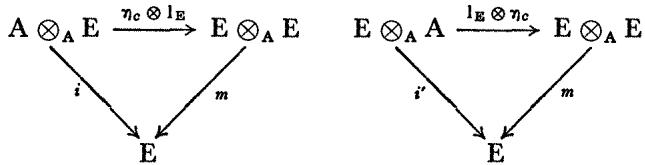
\includegraphics[keepaspectratio]{images/part003_ee0531f1.jpg}}

是交换的（其中 i 和 i' 表示典范同构（II，§3，第 4 号，命题 4））。

设 E 是一个具有单位元 e 的 A-代数，并设 \(\eta = \eta_{e}\) （也记作 \(\eta_{E}\) ）；则 \(\eta(\alpha\beta) = \eta(\alpha)\eta(\beta) = \alpha\eta(\beta)\) ，因为由（2）（第 1 号），

\[
(\alpha e) (\beta e) = (\alpha \beta) e = \alpha (\beta e);
\]

因此 \(\eta\) 是一个 A-代数同态。注意，E 上的 A-模结构可以利用 \(\eta\) 来定义，因为

\[
\alpha x = \eta (\alpha). x \quad \text { for } \alpha \in \mathrm{A}, x \in \mathrm{E}\tag{3}
\]

（其中右端的乘法在 E 中）。同态 \(\eta\) 的像是 E 的一个子代数，其元素与 E 的所有元素交换。同态 \(\eta\) 的核是 A-模 E 中元素 \(e\) 的零化子；由 (3)，它也是 A-模 E 的零化子（II，§ 1，第 12 号）。

当代数 E 含单位元且结合时， \(\eta\) 是一个环同态。反之，设 \(\rho:A\to B\) 是一个环同态，其像 \(\rho(A)\) 包含在 B 的中心内，并设环 A 交换；则在 B 上定义了一个结合且含单位元的 A-代数结构，其定义式为（参见 (3)）

\[
\lambda x = \rho (\lambda). x \quad \text { for } \lambda \in \mathbf {A}, x \in \mathbf {E}.
\]

\subsection{代数的乘积}

设 \((\mathbf{E}_i)_{i\in I}\) 是同一交换环 A 上的一族代数。立即可验证，在乘积集 \(\mathbf{E} = \prod_{i\in I}\mathbf{E}_i\) 上，乘积 A-模结构（II，§ 1，第 5 号）与乘法

\[
\left(\left(x _ {i}\right), \left(y _ {i}\right)\right) \mapsto \left(x _ {i} y _ {i}\right)\tag{4}
\]

定义了一个 A-代数结构；带此结构的集合 E 称为代数族 \((\mathbf{E}_{i})_{i\in I}\) 的积代数。

当所有代数 \(E_{t}\) 都为结合的（相应地，交换的，相应地，含单位元的）时，它们的积也是如此。此外，I，§ 8，第 10 号中所述的所有性质无需修改即可推广到代数的任意乘积。

\subsection{标量的限制与扩张}

设 \(A_{0}\) 和 A 是两个交换环，且 \(\rho:A_{0}\to A\) 是一个环同态。若 E 是一个 A-代数，我们（与 II，§ 1，第 13 号相一致地）用 \(\rho_{*}(E)\) 表示 \(A_{0}\) -模，它由 E 上的加法与外合成律

\[
\lambda . x = \rho (\lambda) x \quad \text { for   all } \lambda \in A _ {0} \text { and   all } x \in E.
\]

E 中的乘法与 \(A_{0}\) -模结构（在 \(\rho_{*}(E)\) 上）一起定义了一个 \(A_{0}\) -代数结构（在 \(\rho_{*}(E)\) 上）。当 \(A_{0}\) 是 A 的子环且 \(\rho\) 为典范单射时，称代数 \(\rho_{*}(E)\) 是由 E 把标量环 A 限制到 \(A_{0}\) 而得到的。作为语言上的滥用，当 \(\rho\) 任意时有时也这样说。

设 F 为一个 \(A_{0}\) -代数。 \(A_{0}\) -代数同态 \(F \to \rho_{*}(E)\) 称为半同态（相对于 \(\rho\) ），或 F 到 A-代数 E 中的 \(\rho\) -同态；若不致混淆，也称为 \(A_{0}\) -同态。若 E, \(E'\) 是两个 A-代数，则每个 A-代数同态 \(E \to E'\) 也是 \(A_{0}\) -代数同态 \(\rho_{*}(E) \to \rho_{*}(E')\) 。

现在考虑两个交换环 A 和 B 以及一个环同态 \(\rho: \mathbf{A} \to \mathbf{B}\) 。对每个 A-模 E，由 E 把标量环 A 扩张到 B 而得到的 B-模 \(\rho^{*}(\mathbf{E}) = \mathbf{E} \otimes_{\mathbf{A}} \mathbf{B}\) 已经定义（II，§ 5，第 1 号）。若 E 还是一个 A-代数，我们要在 \(\rho^{*}(\mathbf{E})\) 上定义一个 B-代数结构。为此，注意到 \((\mathbf{E} \otimes_{\mathbf{A}} \mathbf{B}) \otimes_{\mathbf{B}} (\mathbf{E} \otimes_{\mathbf{A}} \mathbf{B})\) 典范同构于 \((\mathbf{E} \otimes_{\mathbf{A}} \mathbf{E}) \otimes_{\mathbf{A}} \mathbf{B}\) （II，§ 5，第 1 号，命题 3）。若 \(m: \mathbf{E} \otimes_{\mathbf{A}} \mathbf{E} \to \mathbf{E}\) 定义 E 上的乘法，则映射 \(m \otimes l_{\mathbf{B}}: (\mathbf{E} \otimes_{\mathbf{A}} \mathbf{E}) \otimes_{\mathbf{A}} \mathbf{B} \to \mathbf{E} \otimes_{\mathbf{A}} \mathbf{B}\) 便典范地等同于一个 B-线性映射

\[
m ^ {\prime}: \rho^ {*} (\mathbf {E}) \otimes_ {\mathbf {B}} \rho^ {*} (\mathbf {E}) \rightarrow \rho^ {*} (\mathbf {E})
\]

它定义了 \(\rho^{*}(\mathbf{E})\) 上所要的 B-代数结构。于是

\[
(x \otimes \beta) (x ^ {\prime} \otimes \beta^ {\prime}) = (x x ^ {\prime}) \otimes (\beta \beta^ {\prime})\tag{5}
\]

对 \(x, x'\) （属于 \(\mathbf{E}\) ）与 \(\beta\) 、 \(\beta'\) （属于 \(\mathbf{B}\) ）成立，这便是所要的 B-代数结构。称 B-代数 \(\rho^*(\mathbf{E})\) 为由 A-代数 \(\mathbf{E}\) 通过把标量环 \(\mathbf{A}\) 扩张到 \(\mathbf{B}\) （借助 \(\rho\) ）而得到的代数。它也记作 \(\mathrm{E}_{(\mathbf{B})}\) 或 \(\mathbf{E} \otimes_{\mathbf{A}} \mathbf{B}\) 。当 \(\mathbf{E}\) 为结合的（相应地，交换的，相应地，含单位元的）时， \(\rho^*(\mathbf{E})\) 亦然。

对每个 A-代数 E，典范映射 \(\phi_{\mathbf{E}}: x \mapsto x \otimes 1\) （由 E 到 \(\mathrm{E}_{(\mathbf{B})}\) ）是一个代数的 A-同态。此外，对每个 B-代数 F 和每个 A-同态 \(f: \mathbf{E} \to \mathbf{F}\) ，存在唯一的 B-同态 \(\bar{f}: \mathbf{E}_{(\mathbf{B})} \to \mathbf{F}\) ，使得 \(\bar{f}(x \otimes 1) = f(x)\) 对所有 \(x \in \mathbf{E}\) 成立。

第一个断言由 \(\mathrm{E}_{(\mathrm{B})}\) 中乘法的定义直接得出，该定义给出 \((x\otimes1)(x'\otimes1)=(xx')\otimes1\) （对 \(x\in E\) 与 \(x'\in E\) ）。 B-线性映射 \(\bar{f}\) ——它由 \(\mathrm{E}_{(\mathrm{B})}\) 到 F 中、满足关系 \(\bar{f}(x\otimes1)=f(x)\) （对所有 \(x\in E\) ）——的存在性与唯一性由 II，§ 5，第 1 号，命题 1 得出；于是只需验证 \(\bar{f}(yy')=\bar{f}(y)\bar{f}(y')\) 对 y 与 \(y'\) （ \(\mathrm{E}_{(\mathrm{B})}\) 中的）成立；由于形如 \(x\otimes1\) （其中 \(x\in E\) ）的元素生成 B-模 \(\mathrm{E}_{(\mathrm{B})}\) ，只需考虑 \(y=x\otimes1\) , \(y'=x'\otimes1\) （其中 \(x\in E\) , \(x'\in E\) ）的情形；由于 \(yy'=(xx')\otimes1\) ，关系 \(\bar{f}(yy')=\bar{f}(y)\bar{f}(y')\) 便由 \(f(xx')=f(x)f(x')\) 得出。

也可以说 \(f \mapsto \bar{f}\) 是一个典范双射

\[
\operatorname{Hom} _ {\mathrm{A-alg.}} (\mathrm{E}, \rho_ {*} (\mathrm{F})) \rightarrow \operatorname{Hom} _ {\mathrm{B-alg.}} (\rho^ {*} (\mathrm{E}), \mathrm{F}).\tag{6}
\]

由 \(E_{(B)}\) 与 \(\phi_{E}\) 组成的有序对因此是泛映射问题（《集合论》，IV，§ 3，第 1 号）的一个解，其中 \(\Sigma\) 是 B-代数结构这个种类，而 \(\alpha\) -映射是 E 到 B-代数中的 A-同态。

推论。设 E, E' 为两个 A-代数；对代数的每个 A-同态 \(u: E \to E'\) ， \(u \otimes l_{B}\) 是使图表交换的唯一的代数 B-同态 v: \(E \otimes_{A} B \to E' \otimes_{A} B\)

\[
\begin{array}{c} \mathrm{E} \xrightarrow {\phi_ {\mathrm{E}}} \mathrm{E} \otimes_ {\mathrm{A}} \mathrm{B} \\ u \Biggl \downarrow \\ \mathrm{E} ^ {\prime} \xrightarrow [ \phi_ {\mathrm{E} ^ {\prime}} ]{} \mathrm{E} ^ {\prime} \otimes_ {\mathrm{A}} \mathrm{B} \end{array}
\]

设 C 为第三个交换环，且 \(\sigma: B \to C\) 为一个环同态；立即可见，典范 C-同态

\[
\sigma^ {*} (\rho^ {*} (\mathbf {E})) \rightarrow (\sigma \circ \rho) ^ {*} (\mathbf {E})
\]

把 \((x\otimes 1)\otimes 1\) 映为 \(x\otimes 1\) （对所有 \(x\in \mathbf{E}\) ）者（II，§ 5，第 1 号，命题 2）是一个代数同构。

\subsection{代数的逆向极限与正向极限}

设 I 是一个预序集， \((\mathbf{A}_{i},\phi_{ij})\) 是以 I 为指标集的交换环的逆向系统。设 \((\mathbf{E}_{i},f_{ij})\) 是以 I 为指标集的 \(A_{i}\) -模的逆向系统（II，§ 6，第 1 号），并进一步假设每个 \(E_{i}\) 具有 \(A_{i}\) -代数结构，且对 \(i\leqslant j,f_{ij}\) 是代数的 \(A_{j}\) -同态（相对于 \(\phi_{ij}\) ）（第 5 号）。设 \(A=\varprojlim A_{i}\) 与 \(E=\varprojlim E_{i}\) ，后者具有 A-模结构，即诸 \(\mathbf{A}_i\) -模 \(\mathbf{E}_i\) 的结构的逆向极限（II，§ 6，第 1 号）；立即可验证， \(\mathbf{E}\) 上的合成律——把诸 \(\mathbf{E}_i\) 视为乘法下的广群（I，§ 10，第 1 号）而取其逆向极限——连同 \(\mathbf{E}\) 上的 A-模结构，在 \(\mathbf{E}\) 上定义了一个 A-代数结构； \((\mathbf{E}_i, f_{ij})\) 称为 \(\mathbf{A}_i\) -代数的逆向系统，而 A-代数 \(\mathbf{E}\) 称为其逆向极限。若 \(f_i: \mathbf{E} \to \mathbf{E}_i\) , \(\phi_i: \mathbf{A} \to \mathbf{A}_i\) 为典范映射，则 \(f_i\) 是代数的 A-同态（相对于 \(\phi_i\) ）。若诸 \(\mathbf{E}_i\) 结合（相应地，交换），则 \(\mathbf{E}\) 亦然；若每个 \(\mathbf{E}_i\) 具有单位元 \(e_i\) 且 \(f_{ij}(e_j) = e_i\) （对 \(i \leqslant j\) ），则 \(e = (e_i)\) 是代数 \(\mathbf{E}\) 的单位元。

设 \((\mathbf{E}_{i}^{\prime}, f_{ij}^{\prime})\) 是 \(A_{i}\) -代数的另一个逆向系统，且对所有 i 令 \(u_{i}: E_{i} \to E_{i}^{\prime}\) 为 \(A_{i}\) -代数同态，这些映射构成一个逆向系统；则 \(u = \lim u_{i}\) 是一个 A-代数同态。

现在假设所有的 \(A_{i}\) 都等于同一个交换环 A，且诸 \(\phi_{ij}\) 等于 \(Id_{A}\) ，于是 \(E = \lim E_{i}\) 是一个 A-代数。设 F 是一个 A-代数，且对所有 \(i \in I\) ，设 \(u_{i}: F \to E_{i}\) 是一个 A-代数同态，使得 \((u_{i})\) 是一个映射的逆向系统；则 \(u = \lim u_{i}\) 是代数 F 到代数 E 中的同态。反之，对每个 A-代数同态 \(v: F \to E\) ，族 \(v_{i} = f_{i} \circ v\) 是一个 A-代数同态的逆向系统，使得 \(v = \lim v_{i}\) 。此外，由于记 \(\bar{f}_{ij} = \text{Hom}(1_{\text{F}}, f_{ij})\) , \((\text{Hom}_{\text{A-alg.}}(\text{F}, \text{E}_i), \bar{f}_{ij})\) 显然是一个集合的逆向系统，可见上述评注也可以表述为：典范映射 \(v \mapsto (f_i \circ v)\) 是一个双射

\[
l _ {\mathrm{F}}: \operatorname{Hom} _ {\mathrm{A-alg.}} (\mathrm{F}, \varprojlim \mathrm{E} _ {i}) \rightarrow \varprojlim \operatorname{Hom} _ {\mathrm{A-alg.}} (\mathrm{F}, \mathrm{E} _ {i}).
\]

此外，对于每一个 A-代数同态 \(w: \mathbf{F} \to \mathbf{F}'\) ，

\[
\bar {w} _ {i} = \operatorname{Hom} (w, 1 _ {\mathrm{E} _ {i}}): \operatorname{Hom} _ {\mathrm{A-alg.}} (\mathrm{F} ^ {\prime}, \mathrm{E} _ {i}) \rightarrow \operatorname{Hom} _ {\mathrm{A-alg.}} (\mathrm{F}, \mathrm{E} _ {i})
\]

构成映射的逆向系统，且图表

\[
\begin{array}{c} \operatorname{Hom} _ {\mathrm{A-alg.}} (\mathrm{F} ^ {\prime}, \lim \mathrm{E} _ {i}) \xrightarrow {l _ {\mathbf {F} ^ {\prime}}} \lim \operatorname{Hom} _ {\mathrm{A-alg.}} (\mathrm{F} ^ {\prime}, \mathrm{E} _ {i}) \\ \operatorname{Hom} (w, 1 _ {\mathbf {E}}) \Biggl \downarrow \qquad \qquad \qquad \qquad \qquad \qquad \qquad \qquad \qquad \qquad \qquad \qquad \qquad \qquad \qquad \qquad \qquad \qquad \qquad \qquad \qquad \qquad \qquad \qquad \qquad \qquad \qquad \qquad \qquad \qquad \qquad \qquad \qquad \qquad \\ \operatorname{Hom} _ {\mathrm{A-alg.}} (\mathrm{F}, \lim \mathrm{E} _ {i}) \xrightarrow {l _ {\mathbf {F}}} \lim \operatorname{Hom} _ {\mathrm{A-alg.}} (\mathrm{F}, \mathrm{E} _ {i}) \end{array}
\]

是交换的。

现在假设 I 是右有向的。考虑交换环的正向系统 \((\mathbf{A}_i, \phi_{ji})\) 与正向系统 \((\mathbf{E}_i, f_{ji})\) （ \(\mathbf{A}_i\) -模的），均以 I 为指标集；假设每个 \(\mathbf{E}_i\) 具有 \(\mathbf{A}_i\) -代数结构，且对 \(i \leqslant j\) ， \(f_{ji}\) 是代数的 \(\mathbf{A}_i\) -同态（相对于 \(\phi_{ji}\) ）（第 5 号）。设 \(\mathbf{A} = \varinjlim \mathbf{A}_i\) , \(\mathbf{E} = \varinjlim \mathbf{E}_i\) ； \(\mathbf{E}\) 具有 A-模结构，即诸 \(\mathbf{A}_i\) -模 \(\mathbf{E}_i\) 的结构的正向极限（II，§ 6，第 2 号）；此外，E 上的合成律——把诸 \(E_{i}\) 视为乘法下的广群（I，§ 10，第 3 号）而取其正向极限——连同 E 上的 A-模结构，在 E 上定义了一个 A-代数结构； \((\mathbf{E}_{i}, f_{jt})\) 称为 \(A_{i}\) -代数的正向系统，而 A-代数 E 称为其正向极限。若 \(f_{i}: E_{i} \to E\) , \(\phi_{i}: A_{i} \to A\) 为典范映射，则 \(f_{i}\) 是代数的 \(A_{i}\) -同态（相对于 \(\phi_{i}\) ）。若诸 \(E_{i}\) 结合（相应地，交换），则 E 亦然；若每个 \(E_{i}\) 具有单位元 \(e_{i}\) 且 \(f_{jt}(e_{i}) = e_{j}\) （对 \(i \leqslant j\) ），则 E 具有单位元 e，使得 \(f_{i}(e_{i}) = e\) 对所有 \(i \in I\) 成立。

设 \((\mathbf{E}_i', f_{ji}')\) 是 \(\mathbf{A}_i\) -代数的另一个正向系统，且对所有 \(i\) ，设 \(u_i: \mathbf{E}_i \to \mathbf{E}_i'\) 为 \(\mathbf{A}_i\) -代数同态，这些映射构成一个正向系统；则 \(u = \lim u_i\) 是一个 \(\mathbf{A}\) -代数同态。

现在假设所有的环 \(\mathbf{A}_i\) 都等于同一个环 \(\mathbf{A}\) ，且诸 \(\phi_{ji}\) 等于 \(\mathrm{Id}_{\mathbf{A}}\) ，于是 \(\mathbf{E} = \varinjlim \mathbf{E}_i\) 是一个 A-代数。设 \(\mathbf{F}\) 是一个 A-代数，且对所有 \(i\) ，设 \(u_i: \mathbf{E}_i \to \mathbf{F}\) 是一个 A-代数同态，使得 \((u_i)\) 是一个映射的正向系统；则 \(u = \varinjlim u_i\) 是代数 \(\mathbf{E}\) 到代数 \(\mathbf{F}\) 中的同态。反之，对每个 A-代数同态 \(v: \mathbf{E} \to \mathbf{F}\) ，族 \(v_i = v \circ f_i\) 是一个 A-代数同态的正向系统，使得 \(v = \varinjlim v_i\) 。此外，由于记 \(\bar{f}_{ij} = \operatorname{Hom}(f_{ij}, 1_F)\) , \((\operatorname{Hom}_{\mathbf{A-alg}}(\mathbf{E}_i, \mathbf{F}), \bar{f}_{ij})\) 显然是一个集合的逆向系统，可见上述评注也可以表述为：典范映射 \(v \mapsto (v \circ f_i)\) 是一个双射

\[
d _ {\mathrm{F}}: \operatorname{Hom} _ {\mathrm{A-alg.}} (\varinjlim \mathrm{E} _ {i}, \mathrm{F}) \rightarrow \varprojlim \operatorname{Hom} _ {\mathrm{A-alg.}} (\mathrm{E} _ {i}, \mathrm{F}).
\]

进一步地，对于每个A-代数同态 \(w: F \rightarrow F'\) ，

\[
\bar {w} _ {i} = \operatorname{Hom} (1 _ {\mathrm{E} _ {i}}, w): \operatorname{Hom} _ {\mathrm{A-alg.}} (\mathrm{E} _ {i}, \mathrm{F}) \rightarrow \operatorname{Hom} _ {\mathrm{A-alg.}} (\mathrm{E} _ {i}, \mathrm{F} ^ {\prime})
\]

构成映射的逆向系统，且图表

\[
\begin{array}{l} \operatorname{Hom} _ {\mathrm{A-alg.}} (\varinjlim \mathrm{E} _ {i}, \mathrm{F}) \xrightarrow {d _ {\mathrm{F}}} \varprojlim \operatorname{Hom} _ {\mathrm{A-alg.}} (\mathrm{E} _ {i}, \mathrm{F}) \\ \operatorname{Hom} (1 _ {\mathrm{E}}, w) \Biggl \downarrow \qquad \qquad \qquad \qquad \qquad \qquad \qquad \qquad \qquad \qquad \qquad \qquad \qquad \qquad \qquad \qquad \qquad \qquad \qquad \qquad \varprojlim \varpi_ {i} \\ \operatorname{Hom} _ {\mathrm{A-alg.}} (\varinjlim \mathrm{E} _ {i}, \mathrm{F} ^ {\prime}) \xrightarrow {d _ {\mathrm{F} ^ {\prime}}} \varprojlim \operatorname{Hom} _ {\mathrm{A-alg.}} (\mathrm{E} _ {i}, \mathrm{F} ^ {\prime}) \end{array}
\]

是交换的。

\subsection{代数的基。乘法表}

根据定义，A-代数 E 的基就是 E 的 A-模结构的基。设 \((a_{i})_{i\in I}\) 是 E 的一组基；存在唯一的由环 A 的元素组成的族 \((\gamma_{ij}^{k})_{(i,j,k)\in I\times I\times I}\) ，使得对每个有序对 \((i,j)\in I\times I\) ， \(k\in I\) 中使 \(\gamma_{ij}^{k}\neq 0\) 者只有有限多个，且

\[
a _ {i} a _ {j} = \sum_ {k \in \mathbf {I}} \gamma_ {i j} ^ {k} a _ {k}.\tag{7}
\]

诸 \(\gamma_{ij}^{k}\) 称为代数 E 关于基 \((a_{i})\) 的结构常数，而关系式 (7) 构成代数 E （相对于基 \((a_{i})\) ）的乘法表。

关系式（7）可以想象为将这些关系式的右端排列在一个方形表格中写出。

\(\cdots\)

\(a_j\)

\(\cdots\)

\(\vdots\)

\(a_j\)

\(\sum_{k} \gamma_{ij}^{k} a_k\)

\(\vdots\)

这里约定，第 i 行第 j 列处的元素等于乘积 \(a_{i}a_{j}\) 。

反之，给定一个 A-模 E、E 的基 \((a_{i})_{i\in I}\) 以及 A 的元素的一个族 \((\gamma_{ij}^{k})\) ，使得对每个有序对 \((i,j)\in I\times I\) ， \(k\in I\) 中使 \(\gamma_{ij}^{k}\neq 0\) 者只有有限多个，则在 E 上存在唯一的 A-代数结构使关系式 (7) 成立，因为 A-模 \(\mathbf{E}\otimes_{\mathbf{A}}\mathbf{E}\) 是自由的，且以 \((a_{i}\otimes a_{j})_{(i,j)\in I\times I}\) 为基（参见 II，§ 3，第 7 号，命题 7 的推论 2）。

设 E 是一个 A-代数， \((a_{i})_{i\in I}\) 是 A-模 E 的一个生成系（例如一组基）。要使 E 为结合的，必要且充分的条件是诸 \(a_{i}\) 满足结合性关系

\[
(a _ {i} a _ {j}) a _ {k} = a _ {i} (a _ {j} a _ {k}) \quad \text { for   all } i, j, k\tag{8}
\]

映射 \((x, y, z) \mapsto (xy)z - x(yz)\) 是一个 A-三线性映射

\[
\mathbf {E} \times \mathbf {E} \times \mathbf {E} \rightarrow \mathbf {E}
\]

从而定义了一个 A-线性映射 \(E \otimes_{A} E \otimes_{A} E \to E\) ；若后一映射对所有元素 \(a_{i} \otimes a_{j} \otimes a_{k}\) （它们构成 A-模 \(E \otimes_{A} E \otimes_{A} E\) 的一个生成系）均为零，则它恒为零。

类似地，要使 E 为交换的，必要且充分的条件是诸 \(a_{i}\) 满足交换性关系

\[
a _ {i} a _ {j} = a _ {j} a _ {i} \quad \text { for   all } i, j.\tag{9}
\]

证明是类似的，这次考虑 A-双线性映射 \((x,y)\mapsto xy - yx\) 。最后，要使元素 \(e\in E\) 成为单位元，必要且充分的条件是诸 \(a_{i}\) 满足关系

\[
a _ {i} = e a _ {i} = a _ {i} e \quad \text { for   all } i,\tag{10}
\]

这一次是借助 A-线性映射 \(x \mapsto x - xe\) 与 \(x \mapsto x - ex\) 看出的。

当 \((a_{i})_{i\in I}\) 是 E 的一组基且 \((\gamma_{ij}^{k})\) 是相应的结构常数族时，关系式 (8) 等价于关系式

\[
\sum_ {r} \gamma_ {i j} ^ {r} \gamma_ {r k} ^ {s} = \sum_ {r} \gamma_ {i r} ^ {s} \gamma_ {j k} ^ {r}
\]

对所有 \(i, j, k, s\) 成立。类似地，关系式 (9) 等价于 \(\gamma_{ij}^{k} = \gamma_{ji}^{k}\) （对所有 \(i, j, k\) ）。

设 \((a_{i})_{i\in I}\) 是 A-代数 E 的一组基；若 \(\rho :A\to B\) 是一个环同态，则 \((a_{i}\otimes 1)\) 是 B-代数 \(\rho^{*}(\mathbf{E}) = \mathbf{E}\otimes_{\mathbf{A}}\mathbf{B}\) 的一组基（II，§ 5，第 1 号，命题 4）。若 \((\gamma_{ij}^{k})\) 是关于基 \((a_{i})\) 的结构常数族，则族 \((\rho (\gamma_{ij}^{k}))\) 是 \(\rho^{*}(\mathbf{E})\) 关于基 \((a_{i}\otimes 1)\) 的结构常数族。

\section{代数的例子}

在本段中，A 表示一个交换环。

\subsection{自同态代数}

设 B 是一个带单位元（记为 1）的结合 A-代数，并设 M 是一个右 B-模。我们知道环 \(\mathbf{E} = \operatorname{End}_{\mathbf{B}}(\mathbf{M})\) 在 B 的中心上也具有一个模结构。现在，由 A 到 B 的同态 \(h: \alpha \mapsto \alpha\) . 1 的像包含在 B 的中心中（ \(\S 1\) ，第 1 号）；因此 \(h\) 给 E 一个 A-模结构。此外，对 \(\alpha \in \mathbf{A}\) 与 E 中的 \(f, g\) ，

\[
\alpha (f \circ g) = f \circ (\alpha g) = (\alpha f) \circ g;
\]

因此 E 中的乘法与 E 上的 A-模结构定义了 E 上的一个结合 A-代数结构；M 的恒等映射是该代数的一个单位元。

\subsection{矩阵元素}

设 B 为含单位元的结合 A-代数， \(\mathbf{M}_{n}(\mathrm{B})\) 为 B 上 n 阶方阵的集合（II，§ 10，第 7 号）。则 \(\mathbf{M}_{n}(\mathrm{B})\) 具有 A-模结构，定义为 \(\alpha.(b_{ij})=(\alpha b_{ij})(\alpha\in\mathrm{A},b_{ij}\in\mathrm{B},1\leqslant i\leqslant n,1\leqslant j\leqslant n)\) ；此结构与矩阵乘法在 \(\mathbf{M}_{n}(\mathrm{B})\) 上定义了一个含单位元的结合 A-代数结构。 \(\mathbf{M}_{n}(\mathrm{B})\) 到 \(\operatorname{End}_{\mathrm{B}}(\mathrm{B}_{d}^{n})\) 上的典范双射（II，§ 10，第 7 号）是一个 A-代数同构。

当 B = A 时，A-代数 \(\mathbf{M}_{n}(\mathbf{A})\) 具有由矩阵单位（II，§ 10，第 3 号）组成的典范基 \((E_{ij})\) ；相应的乘法表为

\[
E _ {i j} E _ {h k} = \delta_ {j h} \mathrm{E} _ {i k}.\tag{1}
\]

单位元 \(I_{n}\) 等于 \(\sum_{i=1}^{n} E_{ii}\) 。

\subsection{二次代数}

设 \(\alpha, \beta\) 是 A 的两个元素， \((e_1, e_2)\) 是 \(\mathbf{A}^2\) 的典范基。A 上 \((\alpha, \beta)\) 型的二次代数是指带有由乘法表（§ 1，第 7 号）定义的代数结构的 A-模 \(\mathbf{A}^2\)

\[
e _ {1} ^ {2} = e _ {1}, \qquad e _ {1} e _ {2} = e _ {2} e _ {1} = e _ {2}, \qquad e _ {2} ^ {2} = \alpha e _ {1} + \beta e _ {2}.\tag{2}
\]

一个与二次代数同构的A-代数E也称为二次代数。这等同于说E有一个由两个元素组成的基，其中一个为单位元。

可以证明，每个具有由两个元素组成的基的含单位元 A-代数都是二次代数（习题 1）。

若 A-代数的一个基 \((e_{1}, e_{2})\) 的乘法表为 (2)，则称它为 \((\alpha, \beta)\) 型的基。作为语言上的滥用，当一个二次代数具有 \((\alpha, \beta)\) 型的基时，就说它是 \((\alpha, \beta)\) 型的。

命题 1. 二次代数 E 是结合的且交换的。

E 的交换性由 (2) 中的关系式 \(e_{1}e_{2}=e_{2}e_{1}\) 得出；类似地，要验证结合性，只需验证 \(x(yz)=(xy)z\) 当 x, y, z 各取 \(e_{1}\) 或 \(e_{2}\) 时成立。现在，若 x, y, z 中至少有一个等于 \(e_{1}\) ，则此关系显然成立；对 x=y=z=e₂ 也成立，因为 E 交换；命题得证。

设 \(e\) 表示二次代数 \(\mathbf{E}\) 的单位元， \((e, i)\) 是 \(\mathbf{E}\) 的 \((\alpha, \beta)\) 型基； \(\mathbf{E}\) 的包含 \(e\) 的任何其他基因此形如 \((e, j)\) ，其中 \(j = \gamma e + \delta i\) （II，§ 7，第 2 号，命题 3 的推论）；此外， \((e, j)\) 为 \(\mathbf{E}\) 的基的必要且充分条件是 \(\delta\) 在 \(\mathbf{A}\) 中可逆；该条件显然充分；反之，若 \(i\) 是 \(i\) 在 \(\mathbf{E}/\mathbf{A}e\) 中的典范像，则 \(i\) 与 \(\bar{j} = \delta i\) 都必须构成 \(\mathbf{E}/\mathbf{A}e\) 的基，由此得该条件的必要性。于是

\[
j ^ {2} = (\gamma^ {2} + \alpha \delta^ {2}) e + (2 \gamma \delta + \beta \delta^ {2}) i = (\alpha \delta^ {2} - \gamma^ {2} - \beta \gamma \delta) e + (2 \gamma + \beta \delta) j;
\]

由此看出 E 是以下类型的

\[
(\alpha \delta^ {2} - \gamma^ {2} - \beta \gamma \delta , 2 \gamma + \beta \delta)\tag{3}
\]

对所有可逆的 \(\delta \in \mathbf{A}\) 以及所有 \(\gamma \in \mathbf{A}\) 。特别地，若 \(\mathbf{E}\) 是 \((\alpha, 2\beta')\) 型的，则 E 也是 \((\alpha + \beta'^2, 0)\) 型的，这可由取 \(\gamma = -\beta'\) 与 \(\delta = 1\) 看出。

命题 2. 设 E 是一个二次 A-代数，e 是它的单位元。对所有 \(u \in \mathbf{E}\) ，设 \(\mathrm{T}(u)\) 是自由 A-模 E 的自同态 \(m_u: x \mapsto ux\) 的迹（II，§ 4，第 3 号）。则映射 \(s\) ——定义为 \(s(u) = \mathrm{T}(u)\) . \(e - u\) ——是代数 E 的一个自同构，且 \(s^2(u) = u\) 对所有 \(u \in \mathbf{E}\) 成立。

设 \((e, i)\) 是 E 的 \((\alpha, \beta)\) 型基；则 \(T(e) = 2\) ，从而 \(s(e) = e\) ，且 \(T(i) = \beta\) ，从而 \(s(i) = \beta e - i\) 。于是 \((e, s(i))\) 是 E 的基，其类型由 (3) 给出，其中 \(\gamma = \beta\) 且 \(\delta = -1\) ，这重新给出 \((\alpha, \beta)\) ；由此得出 \(s\) 是代数 E 的自同构。由于 \(m_{s(u)} = sm_u s^{-1}\) ，A-模 E 的自同态 \(m_u\) 与 \(m_{s(u)}\) 具有相同的迹（II，§ 4，第 3 号，命题 3），因此

\[
s ^ {2} (u) = \mathrm{T} (u). e - s (u) = \mathrm{T} (u). e - (\mathrm{T} (u). e - u) = u
\]

对所有 \(u \in E\) 成立。

自同构 \(s\) 称为 A-代数 \(\mathbf{E}\) 的共轭，而 \(s(u)\) 称为 \(u\) 的共轭元。

若 \(u = \xi e + \eta i\) ，其中 \(\xi, \eta\) 属于 \(A\) ，则 \(s(u) = (\xi + \beta \eta)e - \eta i\) ，从而

\begin{enumerate}
\def\labelenumi{(\arabic{enumi})}
\setcounter{enumi}{3}
\tightlist
\item
\end{enumerate}

\[
\mathrm{T} (u) e = u + s (u) = (2 \xi + \beta \eta) e\tag{5}
\]

\[
u. s (u) = (\xi^ {2} + \beta \xi \eta - \alpha \eta^ {2}) e = N (u) e
\]

其中我们记 \(\mathrm{N}(u)=\xi^{2}+\beta\xi\eta-\alpha\eta^{2}\) 。元素 \(\mathrm{T}(u)\) 与 \(\mathrm{N}(u)\) （或当 A 与 Ae 典范地等同时的元素 \(\mathrm{T}(u)e\) 与 \(\mathrm{N}(u)e\) ）分别称为 u 的迹与范数。

当 \(\beta = 0\) 时，上述公式简化为

\[
s (\xi e + \eta i) = \xi e - \eta i, \quad \mathrm{T} (\xi e + \eta i) = 2 \xi , \quad \mathrm{N} (\xi e + \eta i) = \xi^ {2} - \alpha \eta^ {2}. \tag {6}
\]

显然，T 是 E 上的线性形式，N 是 E 上的二次形式（IX，§ 3，第 4 号）。由于 E 交换且结合，由 (5) 可得

\[
\mathrm{N} (u v) = \mathrm{N} (u)) \mathrm{N} (v).\tag{7}
\]

要使 u 在 E 中可逆，必要且充分的条件是 \(\mathrm{N}(u)\) 在 A 中可逆。因为由 \(\mathrm{N}(e)=1\) ，取 \(v=u^{-1}\) 便由 (7) 得出条件的必要性。反之，若 \(\mathrm{N}(u)\) 在 A 中可逆，则由 (5) 知 u 可逆，且

\[
u ^ {- 1} = (\mathrm{N} (u)) ^ {- 1} s (u).\tag{8}
\]

可以证明 \(\mathbf{N}(u)\) 是自同态 \(m_u\) 的行列式（§ 8，第 1 号）（参见 § 9 第 3 号，例 1）。

如下命题给出了交换域上二次代数的结构：

命题 3. 设 E 是一个 \((\alpha, \beta)\) 型的二次 A-代数。

\begin{enumerate}
\def\labelenumi{(\roman{enumi})}
\item
  若 \(\mathbf{A}\) 是一个域，且不包含任何元素 \(\zeta\) 使得 \(\zeta^2 = \alpha + \beta \zeta\) ，则 \(\mathbf{E}\) 是 \(a\) （交换）域（参见 V，§ 3）。
\item
  若环 A 含有元素 \(\zeta\) 使得 \(\zeta^2 = \alpha + \beta\zeta\) ，且 \(\beta - 2\zeta\) 可逆（相应地，为零），则 E 同构于 \(\mathbf{A} \times \mathbf{A}\) （相应地，是 \((0,0)\) 型的）。
\end{enumerate}

我们证明 (i)。设 \(\xi, \eta\) 是 A 的两个元素，且 \(u = \xi e + \eta i\) 。若 \(\eta \neq 0\) ，写 \(\theta = -\xi \eta^{-1}\) ，则由 (5) 得 \(\mathrm{N}(u) = \eta^2 (\theta^2 - \beta \theta - \alpha)\) ，于是由对 A 的假设得 \(\mathrm{N}(u) \neq 0\) ；若 \(\eta = 0\) ，则 \(\mathrm{N}(u) = \xi^2\) 。无论哪种情形，若 \(u \neq 0\) ，则 \(\mathrm{N}(u) \neq 0\) ，从而 \(\mathrm{N}(u)\) 在 A 中可逆，因而 \(u\) 在 E 中可逆。

我们现在证明 (ii)。典范基 \((e_{1}, e_{2})\) （代数 \(A \times A\) 的）是 \((0, 1)\) 型的。我们已见（公式 (3)）E 的类型为

\[
(\alpha \delta^ {2} - \gamma^ {2} - \beta \gamma \delta , 2 \gamma + \beta \delta)
\]

对所有 \(\gamma \in \mathbf{A}\) 以及所有 \(\delta\) （在 \(\mathbf{A}\) 中可逆的）。若 \(\beta - 2\zeta\) 可逆，取 \(\delta = (\beta - 2\zeta)^{-1}\) 与 \(\gamma = -\zeta(\beta - 2\zeta)^{-1}\) ；则 \(2\gamma + \beta\delta = 1\) ，且

\[
\alpha \delta^ {2} - \gamma^ {2} - \beta \gamma \delta = \delta^ {2} (\alpha - \zeta^ {2} + \beta \zeta) = 0;
\]

于是 E 是 \((0,1)\) 型的，从而同构于 A × A。若 \(\beta - 2\zeta = 0\) ，则已指出 E 是 \((\alpha + \zeta^{2}, 0)\) 型的，从而是 \((0,0)\) 型的，因为 \(\alpha + \zeta^{2} = 2\zeta^{2} - \beta\zeta = 0\) 。

\((0,0)\) 型的二次 A-代数也称为 A 上的对偶数代数。

\subsection{凯莱代数}

定义 1. \(\mathbf{A}\) 上的一个凯莱代数是指一个有序对 \((\mathbf{E}, s)\) ，其中 \(\mathbf{E}\) 是 \(\mathbf{A}\) 上的一个带单位元 \(e\) 的代数，而 \(s\) 是 \(\mathbf{E}\) 的一个反自同构，使得

\[
u + s (u) \in \mathrm{A} e \quad \text { and } \quad u. s (u) \in \mathrm{A} e
\]

对所有 \(u \in \mathbf{E}\) 成立。

s 称为凯莱代数 (E, s) 的共轭，而 \(s(u)\) 称为 u 的共轭元。条件 \(u + s(u) \in Ae\) 蕴含 u 与 \(s(u)\) 可交换。我们记

\begin{enumerate}
\def\labelenumi{(\arabic{enumi})}
\setcounter{enumi}{8}
\tightlist
\item
\end{enumerate}

\[
\mathrm{T} (u) = u + s (u)\tag{10}
\]

\[
\mathrm{N} (u) = u. s (u) = s (u). u
\]

而子代数 Ae 的这些元素分别称为 u 的凯莱迹与范数。

由二次代数 E 及其共轭 s（因 E 交换，故 s 是反自同构）（第 3 号）组成的有序对是一个凯莱代数。

设 \((\mathbf{E}, s)\) 是一个凯莱代数；由于 \(s(e) = e\) ，有 \(s(u + s(u)) = u + s(u)\) ，换言之 \(s(u) + s^2(u) = u + s(u)\) ，或等价地

\[
s ^ {2} (u) = u\tag{11}
\]

于是 \(s^{2}\) 是 E 的恒等映射。由此可得

\[
\mathrm{T} (s (u)) = \mathrm{T} (u), \quad \mathrm{N} (s (u)) = \mathrm{N} (u).\tag{12}
\]

最后，关系式 \((u - u)(u - s(u)) = 0\) 给出

\[
u ^ {2} - \mathrm{T} (u). u + \mathrm{N} (u) = 0\tag{13}
\]

对所有 \(u \in \mathbf{E}\) 成立。

命题 4. 设 E 是一个 A-代数，s 与 \(s'\) 是 E 的反自同构，使得 \((E, s)\) 与 \((E, s')\) 是凯莱代数。若 E 有一个包含单位元 e 的基，则 \(s' = s\) 。

显然 \(s'(u) = s(u) = u\) 对所有 \(u \in Ae\) 成立。若 T, N（相应地，T', N'）是 (E, s)（相应地，(E, s')）的迹函数与范数函数，则由 (13) 可得

\[
(\mathrm{T} (u) - \mathrm{T} ^ {\prime} (u)). u - (\mathrm{N} (u) - \mathrm{N} ^ {\prime} (u)) = 0.
\]

设 B 是 E 的一个包含 e 的基，u 是 B 中异于 e 的一个元素；则 \(\mathrm{T}(u) - \mathrm{T}'(u) = 0\) ，从而 \(s(u) = s'(u)\) 。由于 s 与 \(s'\) 在 B 上重合，故二者相等。

在下文中我们将记 \(\bar{u} = s(u)\) ，于是

\[
\left\{ \begin{array}{l l} u + \bar {u} = \mathrm{T} (u), & u \bar {u} = \bar {u} u = \mathrm{N} (u), \quad \bar {\bar {u}} = u \\ \overline {{u + v}} = \bar {u} + \bar {v}, & \overline {{\alpha u}} = \alpha \bar {u}, \quad \overline {{u v}} = \bar {v}. \bar {u} \end{array} \right.\tag{14}
\]

其中 \(u, v\) 属于 \(\mathbf{E}, \alpha \in \mathbf{A}\) ；此外

\[
\mathbf {T} (e) = 2 e, \quad \mathbf {N} (e) = e.\tag{15}
\]

由公式

\[
\mathrm{T} (u v) = u v + \overline {{{{u v}}}} = u v + \bar {v}. \bar {u} = u v + (\mathrm{T} (v) - v) (\mathrm{T} (u) - u),
\]

我们推出

\[
u v + v u = \mathrm{T} (u) v + \mathrm{T} (v) u + (\mathrm{T} (u v) - \mathrm{T} (u) \mathrm{T} (v))\tag{16}
\]

由此，交换 \(u\) 与 \(v\) ，得

\[
\mathbf {T} (v u) = \mathbf {T} (u v).\tag{17}
\]

另一方面， \(\mathrm{N}(u+v)=(u+v)(\bar{u}+\bar{v})=\mathrm{N}(u)+\mathrm{N}(v)+\mathrm{T}(u\bar{v})\) ，从而

\[
\mathrm{T} (v \bar {u}) = \mathrm{T} (u \bar {v}) = \mathrm{N} (u + v) - \mathrm{N} (u) - \mathrm{N} (v).\tag{18}
\]

现在，把 (16) 中的 u 换成 \(\bar{u}\) 便得到

\[
\mathrm{T} (u \bar {v}) = \mathrm{T} (u) \mathrm{T} (v) + \bar {u} v + v \bar {u} - \mathrm{T} (u) v - \mathrm{T} (v) \bar {u} = \mathrm{T} (u) \mathrm{T} (v) - u v - \bar {v}. \bar {u};
\]

从而

\[
\mathrm{T} (v \bar {u}) = \mathrm{T} (u \bar {v}) = \mathrm{N} (u + v) - \mathrm{N} (u) - \mathrm{N} (v) = \mathrm{T} (u) \mathrm{T} (v) - \mathrm{T} (u v).\tag{19}
\]

最后，显然对所有 \(\alpha \in \mathbf{A}\) ，

\[
\mathrm{N} (\alpha u) = \alpha^ {2} \mathrm{N} (u);\tag{20}
\]

特别地 \(\mathbf{N}(2u) = 4\mathbf{N}(u)\) ，于是公式 (19) 给出

\[
(\mathrm{T} (u)) ^ {2} - \mathrm{T} (u ^ {2}) = 2 \mathrm{N} (u).\tag{21}
\]

显然 T 是 (Ae)-模 E 上的线性形式。由于 \((u, v) \mapsto \mathrm{T}(v\bar{u})\) 是该模上的双线性形式，由 (18) 与 (20) 可知 N 是一个二次型（参见 IX，§ 3，第 4 号）。

\subsection{凯莱代数的构造。四元数}

设 \((\mathbf{E}, s)\) 是 A 上的一个凯莱代数（对它我们将使用第 4 号的记号），并设 \(\gamma \in \mathbf{A}\) 。设 F 是 A 上的这样的代数：其底模为 \(\mathbf{E} \times \mathbf{E}\) ，乘法由下式定义

\[
(x, y) (x ^ {\prime}, y ^ {\prime}) = (x x ^ {\prime} + \gamma \bar {y} ^ {\prime} y, y \bar {x} ^ {\prime} + y ^ {\prime} x);\tag{22}
\]

显然 \((e,0)\) 是 F 的单位元，且 \(E \times \{0\}\) 是 F 的一个与 E 同构的子代数；在下文中我们把它与 E 等同，于是 \(x \in E\) 与 \((x,0)\) 等同，特别地，e 与 F 的单位元等同。

设 \(t\) 是 \(\mathbf{F}\) 的由下式定义的置换

\begin{enumerate}
\def\labelenumi{(\arabic{enumi})}
\setcounter{enumi}{22}
\tightlist
\item
\end{enumerate}

\[
t ((x, y)) = (\bar {x}, - y) \quad (x \in \mathbf {E}, y \in \mathbf {E}).
\]

命题 5. (i) 有序对 \((\mathbf{F}, t)\) 是 \(\mathbf{A}\) 上的一个凯莱代数。

\begin{enumerate}
\def\labelenumi{(\roman{enumi})}
\setcounter{enumi}{1}
\tightlist
\item
  设 \(j = (0, e)\) ，从而 \((x, y) = xe + yj\) （对 \(x \in \mathbf{E}\) ， \(y \in \mathbf{E}\) ）。 \(\mathbf{T}_{\mathbb{F}}\) 与 \(\mathbf{N}_{\mathbb{F}}\) （ \(\mathbf{F}\) 的凯莱迹与范数）由下列公式给出
\end{enumerate}

\[
\mathrm{T} _ {\mathrm{F}} (x e + y j) = \mathrm{T} (x), \quad \mathrm{N} _ {\mathrm{F}} (x e + y j) = \mathrm{N} (x) - \gamma \mathrm{N} (y).\tag{24}
\]

\begin{enumerate}
\def\labelenumi{(\roman{enumi})}
\setcounter{enumi}{2}
\tightlist
\item
  要使 F 为结合的，必要且充分的条件是 E 为结合的且交换的。
\end{enumerate}

对 \((x,y)\in \mathbf{F},\)

\begin{enumerate}
\def\labelenumi{(\arabic{enumi})}
\setcounter{enumi}{24}
\tightlist
\item
\end{enumerate}

\[
\begin{array}{r l r} & & {(x, y) + t ((x, y)) = (x + \bar {x}, 0) = \mathrm{T} (x) e} \\ & & {(x, y) t ((x, y)) = (x, y) (\bar {x}, - y) = (x \bar {x} - \gamma \bar {y} y, y \bar {\bar {x}} - y x)} \\ & & {= (\mathrm{N} (x) - \gamma \mathrm{N} (y), 0) = (\mathrm{N} (x) - \gamma \mathrm{N} (y)) e.} \end{array}\tag{26}
\]

因此要证明 (i) 与 (ii)，只需证明 t 是 F 的一个反自同构。显然 t 是一个 A-线性双射。另一方面，

\[
\begin{array}{r l} t ((x, y) \cdot (x ^ {\prime}, y ^ {\prime})) & = t ((x x ^ {\prime} + \gamma \bar {y} ^ {\prime} y, y \bar {x} ^ {\prime} + y ^ {\prime} x)) = (\bar {x} ^ {\prime} \bar {x} + \gamma \bar {y} y ^ {\prime}, - y \bar {x} - y ^ {\prime} x) \\ & = (\bar {x} ^ {\prime}, - y ^ {\prime}) (\bar {x}, - y) = t ((x ^ {\prime}, y ^ {\prime})) t ((x, y)) \end{array}
\]

从而 \(t\) 是一个反自同构。

还需证明 (iii)。由于 E 被等同于 F 的一个子代数，可以假设 E 是结合的。设 \(u = (x, y)\) , \(u' = (x', y')\) , \(u'' = (x'', y'')\) 为 F 的元素。则

\[
\left\{ \begin{array}{l} (u u ^ {\prime}) u ^ {\prime \prime} = ((x x ^ {\prime} + \gamma \bar {y} ^ {\prime} y) x ^ {\prime \prime} + \gamma \bar {y} ^ {\prime \prime} (\bar {y} x ^ {\prime} + y ^ {\prime} x), \\ \qquad \qquad \qquad \qquad \qquad \qquad \qquad \qquad \qquad \qquad (y \bar {x} ^ {\prime} + y ^ {\prime} x) \bar {x} ^ {\prime \prime} + y ^ {\prime \prime} (x x ^ {\prime} + \gamma \bar {y} ^ {\prime} y)) \\ u (u ^ {\prime} u ^ {\prime \prime}) = (x (x ^ {\prime} x ^ {\prime \prime} + \gamma \bar {y} ^ {\prime \prime} y ^ {\prime}) + (\gamma (x ^ {\prime \prime} \bar {y} ^ {\prime} + \bar {x} ^ {\prime} \bar {y} ^ {\prime \prime}) y, \\ \qquad \qquad \qquad \qquad \qquad \qquad \qquad \qquad \qquad \qquad y (\bar {x} ^ {\prime \prime} \bar {x} ^ {\prime} + \gamma \bar {y} ^ {\prime} y ^ {\prime \prime}) + (y ^ {\prime} \bar {x} ^ {\prime \prime} + y ^ {\prime \prime} x ^ {\prime}) x). \end{array} \right.\tag{27}
\]

检查这些公式可知，E 的交换性蕴含 F 的结合性。反之，若 F 是结合的，则把公式 (27) 应用于 \(y = y' = 0\) , \(x'' = 0\) 与 \(y'' = e\) 便得 \((0, x'x) = (0, xx')\) ，即 \(x'x = xx'\) 对 E 中所有 \(x, x'\) 成立；因此 E 此时是交换的。

还需注意，在上述记号中，当 \(x, y\) 属于 \(\mathbf{E}\) 时，

\begin{enumerate}
\def\labelenumi{(\arabic{enumi})}
\setcounter{enumi}{27}
\tightlist
\item
\end{enumerate}

\[
\begin{array}{r l} y j = j \overline {{y}}, & x (y j) = (y x) j, \quad (x j) y = (x \overline {{y}}) j, \quad (x j) (y j) = \overline {{y}} x e \\ & j ^ {2} = e. \end{array}\tag{29}
\]

凯莱代数 \((\mathbf{F}, t)\) 称为 \((\mathbf{E}, s)\) 的由 \(\gamma\) 所定义的凯莱扩张。

例子。(1) 若取 \(\mathbf{E} = \mathbf{A}\) （从而 \(s = 1_{\mathbf{A}}\) ），则代数 \(\mathbf{F}\) 是一个二次 \(\mathbf{A}\) -代数，带有基 \((e,j)\) ，其中 \(j^2 = \gamma e\) 。

\begin{enumerate}
\def\labelenumi{(\arabic{enumi})}
\setcounter{enumi}{1}
\tightlist
\item
  取 E 为 \((\alpha, \beta)\) 型的二次代数，于是 E 的底模为 \(A^{2}\) ，其典范基的乘法表为 (2)（第 3 号）。取 s 为 E 的共轭（第 3 号，命题 2）。于是对所有 \(\gamma \in A\) ， \((E, s)\) 的由 \(\gamma\) 所定义的凯莱扩张 F 称为 \((\alpha, \beta, \gamma)\) 型的四元数代数，由第 3 号命题 1 与上述命题 5，它是结合的；其底模为 \(A^{4}\) ，且若 \((e, i, j, k)\) 表示 \(A^{4}\) 的典范基，则相应的乘法表由
\end{enumerate}

\[
\left\{ \begin{array}{l l} i ^ {2} = \alpha e + \beta i, & i j = k, \qquad i k = \alpha j + \beta k, \\ j i = \beta j - k, & j ^ {2} = \gamma e, \qquad j k = \beta \gamma e - \gamma i, \\ k i = - \alpha j, & k j = \gamma i, \qquad k ^ {2} = - \alpha \gamma e. \end{array} \right.\tag{30}
\]

进一步，对 \(u = \rho e + \xi i + \eta j + \eta k\) （其中 \(\rho, \xi, \eta, \zeta\) 属于 A），我们有（以 \(\bar{u}\) 代替 \(t(u)\) 来记，并将 A 与 Ae 等同）：

\[
\left\{ \begin{array}{c} u = (\rho + \beta \xi) e - \xi i - \eta j - \zeta k \\ \mathrm{T} _ {\mathrm{F}} (u) = 2 \rho + \beta \xi \\ \mathrm{N} _ {\mathrm{F}} (u) = \rho^ {2} + \beta \rho \xi - \alpha \xi^ {2} - \gamma (\eta^ {2} + \beta \eta \zeta - \alpha \zeta^ {2}). \end{array} \right.\tag{31}
\]

公式 (30) 由 (28) 与 (29) 得出，公式 (31) 由 (23) 与 (24) 得出，并考虑到二次代数 E 的诸公式。

于是，当 \(u, v\) 属于 \(\mathbf{F}\) 时，

\[
\mathrm{N} _ {\mathrm{F}} (u v) = \mathrm{N} _ {\mathrm{F}} (u) \mathrm{N} _ {\mathrm{F}} (v)\tag{32}
\]

因为 \(\mathrm{N}_{\mathbb{F}}(uv)=uv.\overline{uv}=uv(\bar{v}.\bar{u})=u(v\bar{v})\bar{u}=(u\bar{u})(v\bar{v})\) ，这由结合性以及 \(\mathrm{N}_{\mathbb{F}}(u)\) 属于 F 的中心这一事实得出。

与四元数代数同构的 A-代数也称为四元数代数；若这样一个代数的基具有乘法表 (30)，则称该基为 \((\alpha, \beta, \gamma)\) 型的基。作为语言上的滥用，当一个四元数代数具有 \((\alpha, \beta, \gamma)\) 型的基时，就说它是 \((\alpha, \beta, \gamma)\) 型的。

当 \(\beta = 0\) 时，公式 (30) 与 (31) 简化为

\[
\left\{ \begin{array}{l l} i ^ {2} = \alpha e, & \quad i j = k, \qquad i k = \alpha j, \\ j i = - k, & \quad j ^ {2} = \gamma e, \qquad j k = - \gamma i, \\ k i = - \alpha i, & \quad k j = \gamma i, \qquad k ^ {2} = - \alpha \gamma e, \end{array} \right.\tag{33}
\]

和

\[
\left\{ \begin{array} {c}\bar {u} = \rho e - \xi i - \eta j - \zeta k \\ \mathrm{T} _ {\mathrm{F}} (u) = 2 \rho \\ \mathrm{N} _ {\mathrm{F}} (u) = \rho^ {2} - \alpha \xi^ {2} - \gamma \eta^ {2} + \alpha \gamma \zeta^ {2}. \\ \end{array} \right.\tag{34}
\]

于是在上述表达式中， \((\alpha, \beta, \gamma)\) 处处被 \((\alpha, \gamma)\) 替换。 \((\alpha, \gamma)\) 型与 \((\gamma, \alpha)\) 型的四元数代数显然同构。

注意，公式 (32) 表明，当 \(-1 \neq 1\) 在 A 中时，F 不是交换的。

取 A 为实数域 \(\mathbf{R}\) 且 \(\alpha = \gamma = -1\) , \(\beta = 0\) ，相应的代数 \(F\) 称为哈密顿四元数代数，记作 \(\mathbf{H}\) 。若 \(u = \rho e + \xi i + \eta j + \zeta k\) （ \(\rho, \xi, \eta, \zeta\) 属于 \(\mathbf{R}\) ）是一个 \(\neq 0\) 的、属于 \(\mathbf{H}\) 的元素，则公式 \(u\bar{u} = \bar{u} u = \rho^2 + \xi^2 + \eta^2 + \zeta^2\) （参见 (34)）表明 \(N(u) \neq 0\) 在 \(\mathbf{R}\) 中，于是 \(u\) 具有一个逆元 \(u^{-1} = N(u)^{-1}\bar{u}\) （在 \(\mathbf{H}\) 中），因而 \(\mathbf{H}\) 是一个非交换域。

\begin{enumerate}
\def\labelenumi{(\arabic{enumi})}
\setcounter{enumi}{2}
\tightlist
\item
  若将 E 取为四元数代数（参见例 2），则由元素 \(\delta \in A\) 所定义的 E 的凯莱扩张一般是非结合的（命题 5）；它称为 A 上的一个八元数代数（参见附录，第 3 号）。
\end{enumerate}

\subsection{一个广群、一个幺半群、一个群的代数}

回忆一下，广群是带有一个合成律的集合（I，§ 1，第 1 号）。设 S 是一个以乘法记号书写的广群，令 \(\mathbf{E} = \mathbf{A}^{(\mathbb{S})}\) 为 S 中元素的形式线性组合构成的 A-模（II，§ 1，第 11 号）；我们知道有一个典范映射 \(s \mapsto e_s\) （由 S 到 \(\mathbf{A}^{(\mathbb{S})}\) 中），使得族 \((e_s)_{s \in \mathbb{S}}\) 是 \(\mathbf{A}^{(\mathbb{S})}\) 的基（称为典范基），于是 \(\mathbf{A}^{(\mathbb{S})}\) 的每个元素都可唯一地写成 \(\sum_{s \in \mathbb{S}} \alpha_s e_s\) 的形式，其中 \((\alpha_s)\) 是 A 的元素的有限支集族。则在 E 上定义一个 A-代数结构，其方法是把典范基的乘法表取为

\[
e _ {s} e _ {t} = e _ {s t}\tag{35}
\]

这样定义的代数 E 称为广群 S 在 A 上的代数。若 \(x = \sum_{s \in S} \xi_{s} e_{s}\) 与 \(y = \sum_{s \in S} \eta_{s} e_{s}\) 是 E 的两个元素，则

\[
x y = \sum_ {s \in \mathbb {S}} \left(\sum_ {t u = s} \xi_ {t} \eta_ {u}\right) e _ {s}.
\]

当 S 是幺半群（相应地，群）时，E 称为 S 在 A 上的幺半群（相应地，群）代数；此时它是一个结合代数（§ 1，第 7 号）；类似地，当 S 是交换幺半群时，其代数是结合的且交换的。最后，若广群 S 具有单位元 \(u\) ，则 \(e_u\) 是代数 E 的单位元；由于元素 \(e_u\) 是自由的，A 于是与 E 的子代数 \(Ae_u\) 等同。

当 \(A \neq \{0\}\) 时，S 有时被等同于它在单射 \(s \mapsto e_{s}\) 下的像，于是 E 的元素可写成 \(\sum_{s \in S} \alpha_{s}s\) ；但当 S 以加法记号书写时，这一等同（若不引起混淆）是不可能的。这时也常以 \(e^{s}\) 代替 \(e_{s}\) 来写。

设 B 是另一个交换环， \(\rho: A \to B\) 是一个环同态；考虑同一广群 S 在 A 上与 B 上的代数 \(E = A^{(S)}\) 与 \(E' = B^{(S)}\) ，并令 \((e_s)_{s \in S}\) 与 \((e_s')_{s \in S}\) 分别为它们的典范基。代数 \(B^{(S)}\) 在 A-线性映射 \(j\) （它使得 \(j(e_s \otimes 1) = e_s'\) 对所有 \(s \in S\) 成立）下典范地等同于代数 \(A^{(S)} \otimes_A B\) ——它由 \(A^{(S)}\) 把标量环扩张到 B 而得到——（II，§ 1，第 11 号，命题 17 的推论 3）。

命题 6. 设 S 为一个广群，F 为一个 A-代数，且 f 为一个同态，它把

S 映入仅带乘法结构的 F。则存在且仅存在一个 A-代数同态 \(\bar{f}:\mathbf{A}^{(\mathbb{S})}\to\mathbf{F}\) 使图表交换

\begin{enumerate}
\def\labelenumi{(\arabic{enumi})}
\setcounter{enumi}{35}
\tightlist
\item
\end{enumerate}

\pandocbounded{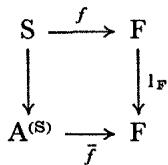
\includegraphics[keepaspectratio]{images/part003_a94682a2.jpg}}

（其中左边的竖直箭头是典范映射 \(s \mapsto e_s\) ）。

设 \(\bar{f}:\mathbf{A}^{(\mathrm{S})}\to\mathbf{F}\) 是唯一的 A-模同态，使得 \(\bar{f}(e_{s})=\bar{f}(s)\) （II，§ 1，第 11 号，命题 17 的推论 3）；只需验证 \(\bar{f}\) 是代数同态，而为此只需证明 \(\bar{f}(e_{s}e_{t})=\bar{f}(e_{s})\bar{f}(e_{t})\) ，它由定义与假设 \(f(st)=f(s)f(t)\) 直接得出。

命题 6 表达了如下事实：由 \(\mathbf{A}^{(\mathbb{S})}\) 与典范映射 \(s\mapsto e_s\) 组成的有序对是泛映射问题（《集合论》，IV，§ 3，第 1 号）的一个解，其中 \(\Sigma\) 是 A-代数结构这一种类，而 \(\alpha\) 映射是把 S 映入一个仅带其乘法律的 A-代数的同态。

推论。设 S, S' 为两个广群， \(g:S\to S'\) 为一个同态。则存在且仅存在一个 A-代数同态 \(u:A^{(S)}\to A^{(S')}\) 使图表交换

\pandocbounded{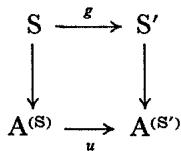
\includegraphics[keepaspectratio]{images/part003_71823134.jpg}}

（其中竖直箭头是典范映射）。

只需把命题 6 应用于取 \(f\) 为复合映射 \(\mathbf{S} \xrightarrow{g} \mathbf{S}' \to \mathbf{A}^{(\mathbf{S}')}\) 的情形。

特别地，若 T 是广群 S（I，§ 1，第 4 号）的稳定子集，则形如 \(\sum_{s\in\mathbf{T}}\alpha_s e_s\) 的元素（属于 \(\mathbf{A}^{(\mathbf{S})}\) ）所成的集合是 \(\mathbf{A}^{(\mathbf{S})}\) 的一个子代数，它典范同构于代数 \(\mathbf{A}^{(\mathbf{T})}\) ，且有时与后者等同。

例。设 V 是一个 A-模，S 是一个在 V 上从左边作用的幺半群；这就是说（I，§ 5，第 1 号），给定了一个映射 \((s, x) \mapsto s.x\) （由 S 到 V），使得 \(s.(x + y) = s.x + s.y\) , \(s.(\alpha x) = \alpha(s.x)\) 与 \(s.(t.x) = (st).x\) 对 \(s, t\) （在 S 中）、 \(x, y\) （在 V 中）与 \(\alpha \in \mathbf{A}\) 成立，且（把 \(e\) 记作 S 的单位元）对 \(x \in V\) 有 e.x = x。写 \(f(s)(x) = s.x\) ，则 f 是 S 到代数 \(\operatorname{End}_{\mathbf{A}}(\mathbf{V})\) （仅带其乘法律）中的一个同态，它把单位元 e 映到单位元 \(1_{V}\) 。应用命题 6，得到一个 A-代数同态 \(\bar{f}: \mathbf{A}^{(\mathbf{S})} \to \operatorname{End}_{\mathbf{A}}(\mathbf{V})\) ，它给出 V 的底群在 \(\mathbf{A}^{(\mathbf{S})}\) 上的一个左模结构。

这使我们能把带算子的交换群的研究归结为模的研究。因为设 M 是一个带算子的交换群，其运算以加法书写，所有外部律以乘法书写。设 \(\Omega\) 为 M 上各个外部律的算子定义域的和集（《集合论》，II，§ 4，第 8 号），其中每个定义域都被典范地等同于 \(\Omega\) 的一个子集。设 \(\mathrm{Mo}(\Omega)\) 为在 \(\Omega\) 上构造的自由幺半群（I，§ 7，第 2 号）；一个作用律

\[
(s, x) \mapsto s. x
\]

在 M 上定义，以 \(\mathrm{Mo}(\Omega)\) 为算子域，通过对 \(\mathrm{Mo}(\Omega)\) 中字 s 的长度作归纳来定义；若 s 的长度为 0，则它是空字 e，我们对所有 \(x \in M\) 写 e.x = x。若 x 的长度为 \(n \geqslant 1\) ，则它可以唯一地写成 s = tu，其中 u 的长度为 n - 1，t 的长度为 1，因此 \(t \in \Omega\) ；随后我们写 s.x = t.(u.x)。对任意两个字 s 与 \(s'\) （在 \(\mathrm{Mo}(\Omega)\) 中），关系 \(s.(s'.x) = (ss').x\) 通过对 s 的长度作归纳来验证。

然后应用上述方法，就在 M 上得到一个左 \(\mathbf{Z}^{(\mathrm{Mo}(\Omega))}\) -模结构，并且不难验证，带算子群论中的通常概念（稳定子群、同态）对带算子的交换群与这样关联于它们的模来说是相同的。

\subsection{自由代数}

定义 2. 设 I 是一个集合；令 M(I)（相应地 Mo(I)，相应地 N \(^{(I)}\) ）表示由 I 导出的自由广群（相应地自由幺半群，相应地自由交换幺半群）。M(I)（相应地 Mo(I)，相应地 N \(^{(I)}\) ）在 A 上的代数称为集合 I 在环 A 上的自由代数（相应地自由结合代数，相应地自由交换结合代数（或作为语言上的滥用，称为自由交换代数））。

我们把 I 在 A 上的自由代数（相应地自由结合代数，相应地自由交换代数）记作 \(\operatorname{Lib}_{\mathbf{A}}(\mathbf{I})\) （相应地 \(\operatorname{Libas}_{\mathbf{A}}(\mathbf{I})\) ，相应地 \(\operatorname{Libasc}_{\mathbf{A}}(\mathbf{I})\) ）。把 I 到 \(\operatorname{M}(\mathbf{I})\) （相应地 \(\operatorname{Mo}(\mathbf{I})\) ，相应地 \(\mathbf{N}^{(\mathbf{I})}\) ）中的典范映射与 \(\operatorname{M}(\mathbf{I})\) （相应地 \(\operatorname{Mo}(\mathbf{I})\) ，相应地 \(\mathbf{N}^{(\mathbf{I})}\) ）到 \(\operatorname{Lib}_{\mathbf{A}}(\mathbf{I})\) （相应地 \(\operatorname{Libas}_{\mathbf{A}}(\mathbf{I})\) ，相应地 \(\operatorname{Libasc}_{\mathbf{A}}(\mathbf{I})\) ）中的典范映射复合，就得到 I 到 \(\operatorname{Lib}_{\mathbf{A}}(\mathbf{I})\) （相应地 \(\operatorname{Libas}_{\mathbf{A}}(\mathbf{I})\) ，相应地 \(\operatorname{Libasc}_{\mathbf{A}}(\mathbf{I})\) ）中的一个典范映射，当 \(A \neq \{0\}\) 时它是单射。我们把元素 \(i \in I\) 在此典范映射下的像记作 \(X_{i}\) ，并称 \(X_{i}\) 为 \(\operatorname{Lib}_{\mathbf{A}}(\mathbf{I})\) （相应地 \(\operatorname{Libas}_{\mathbf{A}}(\mathbf{I})\) ，相应地 \(\operatorname{Libasc}_{\mathbf{A}}(\mathbf{I})\) ）的指标为 i 的未定元。

由于 \(\mathbf{Mo}(\mathbf{I})\) 与 \(\mathbf{N}^{(\mathrm{I})}\) 各有一个单位元， \(\operatorname{Libas}_{\mathbf{A}}(\mathbf{I})\) 与 \(\operatorname{Libasc}_{\mathbf{A}}(\mathbf{I})\)

是含单位元的结合代数，且进一步 \(\operatorname{Libasc}_{\mathbf{A}}(\mathbf{I})\) 是交换的。若 e 是 \(\operatorname{Libas}_{\mathbf{A}}(\mathbf{I})\) （相应地 \(\operatorname{Libasc}_{\mathbf{A}}(\mathbf{I})\) ）的单位元，则映射 \(\alpha \mapsto \alpha e\) 是 A 到 \(\operatorname{Libas}_{\mathbf{A}}(\mathbf{I})\) （相应地 \(\operatorname{Libasc}_{\mathbf{A}}(\mathbf{I})\) ）的中心的一个子环上的同构，该子环与 A 等同（第 1 号）。

命题 7. 设 I 是一个集合，F 是 A 上的一个代数（相应地，含单位元结合代数，相应地，含单位元交换结合代数）。对每个映射 \(f:\mathbf{I}\to\mathbf{F}\) ，存在且仅存在一个同态（相应地，保单位同态） \(\bar{f}\) ，它由 \(\operatorname{Lib}_{\mathbf{A}}(\mathbf{I})\) （相应地 \(\operatorname{Libas}_{\mathbf{A}}(\mathbf{I})\) ，相应地 \(\operatorname{Libasc}_{\mathbf{A}}(\mathbf{I})\) ）到 F 中，使得 \(\bar{f}(\mathbf{X}_{i})=f(i)\) 对所有 \(i\in\mathbf{I}\) 成立。

设 \(F_{m}\) 是通过赋予集合 F 其乘法合成律而得到的广群（相应地，幺半群）。存在且仅存在一个同态（相应地，保单位同态）g，由 M(I)（相应地，Mo(I)，相应地，N \(^{(I)}\) ）到 \(F_{m}\) 中，使得 \(g(i) = f(i)\) 对所有 \(i \in I\) 成立（I，§ 7，第 1、2 与 7 号）；命题 7 随后由第 6 号命题 6 得出。

注记。(1) 我们稍后将定义 \(\operatorname{Libas}_{\mathbf{A}}(\mathbf{I})\) 到自由模 \(\mathbf{A}^{(I)}\) 的张量代数上的一个同构（ \(\S 5\) ，第 5 号），以及 \(\operatorname{Libasc}_{\mathbf{A}}(\mathbf{I})\) 到 \(\mathbf{A}^{(I)}\) 的对称代数上的一个同构（ \(\S 6\) ，第 6 号）。

\begin{enumerate}
\def\labelenumi{(\arabic{enumi})}
\setcounter{enumi}{1}
\item
  设 \(\rho\) 是 A 到交换环 B 中的保单位同态。如已见（§ 2，第 6 号），一个同构 \(\sigma\) 由 \(\rho\) 导出，它把 \(\operatorname{Lib}_{\mathbf{B}}(\mathbf{I})\) （相应地 \(\operatorname{Libas}_{\mathbf{B}}(\mathbf{I})\) ，相应地 \(\operatorname{Libasc}_{\mathbf{B}}(\mathbf{I})\) ）映到代数 \((\operatorname{Lib}_{\mathbf{A}}(\mathbf{I}))_{(\mathbf{B})}\) （相应地 \((\operatorname{Libas}_{\mathbf{A}}(\mathbf{I}))_{(\mathbf{B})}\) ，相应地 \((\operatorname{Libasc}_{\mathbf{A}}(\mathbf{I}))_{(\mathbf{B})}\) ）上，该代数是把标量借助 \(\rho\) 扩张到 B 而得到的；若 \(\mathbf{X}_i^{\mathbf{A}}\) , \(\mathbf{X}_i^{\mathbf{B}}\) 是分别对应于 A 与 B 的指标为 \(i\) 的未定元，则 \(\sigma(\mathbf{X}_i^{\mathbf{B}}) = \mathbf{X}_i^{\mathbf{A}} \otimes 1\) 。
\item
  设 \(J\) 是 \(I\) 的一个子集；我们知道 \(M(J)\) 被等同于广群 \(M(I)\) 的一个稳定子集，因此（第 6 号） \(\operatorname{Lib}_{A}(J)\) 典范地等同于 \(\operatorname{Lib}_{A}(I)\) 的一个子代数，它由诸 \(X_i\) ——满足 \(i \in J\) ——生成；我们说，只有指标属于 \(J\) 的未定元出现在 \(\operatorname{Lib}_{A}(J)\) 的一个元素中。第 6 号中给出的广群代数的定义表明， \(\operatorname{Lib}_{A}(I)\) 是子代数 \(\operatorname{Lib}_{A}(J)\) 的有向族的并，其中 \(J\) 遍历 \(I\) 的有限子集的集合。对 \(\operatorname{Libas}_{A}(I)\) 与 \(\operatorname{Libasc}_{A}(I)\) 有类似的结果。
\item
  对元素 \(s\) —— \(\mathbf{M}(\mathbf{I})\) （相应地 \(\mathbf{Mo}(\mathbf{I})\) ，相应地 \(\mathbf{N}^{(1)}\) ）的——关联它的长度 \(l(s)\) ，这是一个 \(\geqslant 1\) （相应地 \(\geqslant 0\) ）的整数，使得 \(l(ss') = l(s) + l(s')\) （I，§ 7，第 1、2 与 7 号）。若 \(e_s\) 是 \(\operatorname{Lib}_{\mathbf{A}}(\mathbf{I})\) （相应地 \(\operatorname{Libas}_{\mathbf{A}}(\mathbf{I})\) ，相应地 \(\operatorname{Libasc}_{\mathbf{A}}(\mathbf{I})\) ）中对应于 \(s\) 的元素，则元素 \(x = \sum_{s} \alpha_s e_s \neq 0\) （属于 \(\operatorname{Lib}_{\mathbf{A}}(\mathbf{I})\) （相应地 \(\operatorname{Libas}_{\mathbf{A}}(\mathbf{A})\) ，相应地 \(\operatorname{Libasc}_{\mathbf{A}}(\mathbf{I})\) ））的总次数（或简称次数）是诸数 \(l(s)\) 中的最大者，其中 \(s\) 遍历（依假设非空的）满足 \(\alpha_s \neq 0\) 的元素集合。例如，若 \(i, j, k\) 是 \(\mathbf{I}\) 的三个不同元素，则元素 \((\mathrm{X}_t(\mathrm{X}_j\mathrm{X}_k))\mathrm{X}_t - (\mathrm{X}_t\mathrm{X}_j)(\mathrm{X}_k\mathrm{X}_l)\) 是一个 \(\neq 0\) 的、总次数为 4 的元素（在 \(\operatorname{Lib}_{\mathbf{A}}(\mathbf{I})\) 中）。
\end{enumerate}

\subsection{用生成元和关系定义代数}

设 \(\mathbf{F}\) 是 \(\mathbf{A}\) 上的一个代数， \((x_{i})_{i\in I}\) 是 \(\mathbf{F}\) 的元素的一个族。根据第 7 号命题 7，存在唯一的同态 \(f\colon \operatorname{Lib}_{\mathbf{A}}(\mathbf{I})\to \mathbf{F}\) ，使得 \(f(\mathbf{X}_i) = x_i\) 对所有 \(i\in I\) 成立。要使 \(f\) 为满射，必要且充分的条件是 \((x_{i})_{i\in I}\) 是 \(\mathbf{F}\) 的一个生成系。

若 \(\mathbf{U} \in \operatorname{Lib}_{\mathbf{A}}(\mathbf{I})\) ，则 \(f(\mathbf{U})\) 称为 \(\mathbf{F}\) 的、由 \(\mathbf{U}\) 通过把元素 \(x_{i}\) 代入未定元 \(\mathbf{X}_{i}\) 而得到的元素，也称为 \(\mathbf{U}\) 当未定元取值 \(x_{i}\) （就未定元 \(\mathbf{X}_{i}\) 而言）时的值；它通常记作 \(\mathbf{U}((x_{i})_{i \in I})\) ；特别地， \(\mathbf{U}((\mathbf{X}_{i})_{i \in I}) = \mathbf{U}\) 。若 \(\lambda\) 是 \(\mathbf{F}\) 到一个代数 \(\mathbf{F}'\) （ \(\mathbf{A}\) 上的）中的同态，则

\[
\lambda (\mathrm{U} ((x _ {i}) _ {i \in \mathrm{I}})) = \mathrm{U} ((\lambda (x _ {i})) _ {i \in \mathrm{I}}).
\]

特别考虑以下情形： \(\mathrm{F} = \operatorname{Lib}_{\mathbf{A}}(\mathbf{J})\) ，其中 J 是另一个集合；对元素的每一个族 \((\mathrm{H}_{i})_{i \in I}\) （属于 \(\operatorname{Lib}_{\mathbf{A}}(\mathbf{J})\) ）以及每个族 \((y_{j}')_{j \in J}\) （属于 A-代数 \(F'\) ），

\[
\mathrm{U} ((\mathrm{H} _ {i}) _ {i \in I})) ((y _ {j} ^ {\prime}) _ {j \in J}) = \mathrm{U} ((\mathrm{H} _ {i} ((y _ {j} ^ {\prime}) _ {j \in J})) _ {i \in I}).\tag{37}
\]

在上述记号中， \(\operatorname{Lib}_{\mathbf{A}}(\mathbf{I})\) 的每个使得 \(\mathrm{U}((x_{i})_{i\in\mathbf{I}})=0\) （亦即满足 \(f(\mathrm{U})=0\) ）的元素 U，称为族 \((x_{i})_{i\in\mathbf{I}}\) 在 F 中的关系子。由这些元素组成的双边理想 \(\operatorname{Ker}(f)\) 称为 \((x_{i})\) 的关系子理想。

设 \((\mathbf{R}_j)_{j\in J}\) 是 \(\operatorname{Lib}_{\mathbf{A}}(\mathbf{I})\) 的元素的一个族。 \(((x_i)_{i\in I}, (\mathbf{R}_j)_{j\in J})\) 称为代数 \(F\) 的一个表出，如果 \((x_i)_{i\in I}\) 是 \(F\) 的生成系，且 \(\operatorname{Lib}_{\mathbf{A}}(\mathbf{I})\) 的由诸 \(\mathbf{R}_j\) 生成的双边理想等于族 \((x_i)_{i\in I}\) 的关系子理想； \(x_i\) 称为生成元，而 \(\mathbf{R}_j\) 称为该表出的关系子。

现在考虑任意的集合 I 与元素的一个族 \((\mathbf{R}_j)_{j\in J}\) （属于 \(\operatorname{Lib}_{\mathbf{A}}(\mathbf{I})\) ）。 \(\operatorname{Lib}_{\mathbf{A}}(\mathbf{I})\) 关于由族 \((\mathbf{R}_j)\) 生成的双边理想的商代数 E，称为由生成系 I 经关系子族 \((\mathbf{R}_j)_{j\in J}\) 约束而定义的泛代数。显然，若 \(\overline{\mathbf{X}}_i\) 表示 \(\mathbf{X}_i\) 在 E 中的像，

\[
\left(\left(\overline {{\mathbf {X}}} _ {i}\right) _ {i \in I}, \left(\mathbf {R} _ {j}\right) _ {j \in J}\right)
\]

是 E 的一个表出。此外，若 \((x_{i})_{i\in I}\) 是一个代数 F 的元素族，且 \(\mathbf{R}_j((x_i)_{i\in I}) = 0\) 对所有 \(j\in J\) 成立，则存在唯一的同态 \(g:\mathbf{E}\to \mathbf{F}\) ，使得 \(g(\overline{\mathbf{X}}_i) = x_i\) 对所有 \(i\in I\) 成立；要使 \(((x_i)_{i\in I},(\mathbf{R}_j)_{j\in J})\) 是 F 的一个表出，必要且充分的条件是 \(g\) 为双射。

这些评注为下面的语言滥用提供了正当性：不说“ \(((x_i)_{i \in I}, (R_j)_{j \in J})\) 是 F 的一个表出”，也说“F 是由生成元 \(x_i\) 在关系 \(R_j((x_i)_{i \in I}) = 0\) 约束下生成的代数”。当 \(R_j\) 形如 \(P_j - Q_j\) 时，也说“F 是由 \(x_i\) 在关系 \(P_j((x_i)) = Q_j((x_i))\) 约束下生成的代数”。

设 H 是一个集合；我们将说 \(\operatorname{Lib}_{\mathbf{A}}(\mathbf{H})\) 的元素 S 是 A-代数 F 的一个泛关系子，如果 \(\mathrm{S}((x_{h})_{h\in\mathbb{H}})=0\) 对以 H 为指标集的 F 的元素的每个族 \((x_{h})_{h\in\mathbb{H}}\) 成立。

例子。(1) 取 \(\mathbf{H} = \{1,2,3\}\) ；承认

\[
(\mathrm{X} _ {1} \mathrm{X} _ {2}) \mathrm{X} _ {3} - \mathrm{X} _ {1} (\mathrm{X} _ {2} \mathrm{X} _ {3})
\]

作为泛关系子的代数是结合代数。承认 \(X_{1}X_{2}-X_{2}X_{1}\) 作为泛关系子的代数是交换代数。承认泛关系子 \(X_{1}X_{1}\) 与

\[
(\mathrm{X} _ {1} \mathrm{X} _ {2}) \mathrm{X} _ {3} + (\mathrm{X} _ {2} \mathrm{X} _ {3}) \mathrm{X} _ {1} + (\mathrm{X} _ {3} \mathrm{X} _ {1}) \mathrm{X} _ {2}
\]

作为泛关系子的代数是李代数。

设 I 是一个集合；给定元素的一个族 \((\mathrm{S}_{k})_{k\in\mathbb{K}}\) （属于 \(\operatorname{Lib}_{\mathbf{A}}(\mathbf{H})\) ），考虑 \(\operatorname{Lib}_{\mathbf{A}}(\mathbf{I})\) 中形如 \(\mathrm{S}_{k}((\mathrm{U}_{h}))_{h\in\mathbb{H}}\) 的元素组成的集合 T，其中 k 遍历 K，且对每个 \(k,\left(\mathrm{U}_{h}\right)_{h\in\mathbb{H}}\) 遍历 \(\operatorname{Lib}_{\mathbf{A}}(\mathbf{I})\) 的元素的以 H 为指标集的族的集合；再考虑一个以 T 为元素集的族 \((\mathrm{R}_{j})_{j\in\mathbb{J}}\) 。然后令 F 为由生成系 I 经关系子族 \((\mathrm{R}_{j})_{j\in\mathbb{J}}\) 约束而定义的泛代数，并设 \(u:\operatorname{Lib}_{\mathbf{A}}(\mathbf{I})\to\mathbf{F}\) 为典范同态，于是 \(\operatorname{Ker}(u)\) 由形如 \(\mathrm{S}_{k}((\mathrm{U}_{h})_{h\in\mathbb{H}})\) 的元素生成，其中 \(k\in K\) 且 \((\mathrm{U}_{h})_{h\in\mathbb{H}}\) 是 \(\operatorname{Lib}_{\mathbf{A}}(\mathbf{I})\) 的元素的族；显然每个 \(S_{k}\) \((k\in\mathbb{K})\) 都是 F 的一个泛关系子。现在设 \(F'\) 是承认一个生成系 \((x_{i})_{i\in\mathbb{I}}\) 的代数，对它每个 \(S_{k}\) 都是泛关系子，并设 \(u':\operatorname{Lib}_{\mathbf{A}}(\mathbf{I})\to\mathbf{F}'\) 是使得 \(u'(\mathrm{X}_{i})=x_{i}\) （对所有 \(i\in I\) ）成立的同态；显然 \(\operatorname{Ker}(u)\subset\operatorname{Ker}(u')\) ，因此 \(u'\) 可唯一地写成 \(u'=h\circ u\) 的形式，其中 \(h:F\to F'\) 是一个使 \(h(\overline{\mathrm{X}}_{i})=x_{i}\) 对所有 \(i\in I\) 成立的同态。因此，F 称为由生成系 I 定义的、对应于泛关系子族 \((\mathrm{S}_{k})_{k\in\mathbb{K}}\) 的泛代数。作为语言上的滥用，F 有时也称为由 I 生成且满足恒等式 \(\mathrm{S}_{k}((u_{h}))=0\) （对 F 的元素的每个族 \((u_{h})_{h\in\mathbb{H}}\) ）的泛代数。

例 2. 设 \(\mathbf{L}'\) 为由 \(\mathbf{I}\) 生成且满足恒等式 \((uv)w - u(vw) = 0\) （对 \(\mathbf{L}'\) 的元素的每个三元族）的泛代数，并设 \(\mathbf{L}''\) 为由 \(\mathbf{L}'\) 添加单位元而得到的代数；则存在唯一的保单位同构 \(g\) ，它由 \(\mathbf{L}''\) 到 \(\operatorname{Libas}_{\mathbf{A}}(\mathbf{I})\) 上，使得 \(g(\overline{\mathbf{X}}_i) = \mathbf{X}_i\) 对所有 \(i \in \mathbf{I}\) 成立。因为显然 \(\mathbf{L}''\) 是结合的，且同态 \(g\) 的存在性由 \(\mathbf{L}'\) 的定义及其前面的评注得出；但于是显然 \(\mathbf{L}''\) 满足刻画 \(\operatorname{Libas}_{\mathbf{A}}(\mathbf{I})\)

的泛性质（第 7 号，命题 7），由此得出结论。与上述类似的考虑可应用于结合代数（相应地，交换结合代数），同时考虑到以下评注。当上下文充分表明所考虑的代数是含单位元代数时，作为语言上的滥用，一个族 \((x_{i})_{i\in I}\) （它是代数 \(F\) 的元素的族），若由诸 \(x_{i}\) ( \(i\in I\) ) 与单位元生成的子代数等于 \(F\) ，则常称为 \(F\) 的一个生成系。然后设 \(F\) 是 \(A\) 上的一个含单位元结合代数， \((x_{i})_{i\in I}\) 是 \(F\) 的元素的一个族；根据第 7 号命题 7，存在唯一的保单位同态 \(f:\mathrm{Libas}_{\mathbf{A}}(\mathbf{I})\to F\) ，使得 \(f(\mathbf{X}_i) = x_i\) 对所有 \(i\in I\) 成立；若 \(\mathbf{U}\in \mathrm{Libas}_{\mathbf{A}}(\mathbf{I}), f(\mathbf{U})\) 也称为 \(F\) 的、由 \(\mathbf{U}\) 通过把元素 \(x_{i}\) 代入未定元 \(\mathbf{X}_i\) 而得到的元素，并且也记作 \(\mathrm{U}((x_{i})_{i\in I})\) 。于是，关系子、表出与泛关系子的概念可立即搬到结合代数上；只需把 \(\mathrm{Lib}_{\mathbf{A}}(\mathbf{I})\) 处处替换为 \(\mathrm{Libas}_{\mathbf{A}}(\mathbf{I})\) 即可。由生成系 \(I\) 经关系子族 \((\mathbb{R}_j)_{j\in J}\) 约束而定义的泛含单位元结合代数是 \(\mathrm{Libas}_{\mathbf{A}}(\mathbf{I})\) 关于由族 \((\mathbb{R}_j)\) 生成的双边理想的商代数。由生成系 \(I\) 生成的、对应于一族泛关系子的泛含单位元结合代数类似地定义。我们把关于交换结合代数的类似定义的陈述留给读者，只需以 \(\mathrm{Libasc}_{\mathbf{A}}(\mathbf{I})\) 替换 \(\mathrm{Libas}_{\mathbf{A}}(\mathbf{I})\) 即可。

例 3. 设 L' 是由 I 生成且满足恒等式 uv - vu = 0（对 L' 的元素的每个二元族）的泛含单位元结合代数。如例 2 中那样可以看出，L' 典范同构于 \(\text{Libasc}_{\mathbf{A}}(\mathbf{I})\) 。

\subsection{多项式代数}

设 B 是一个含单位元的交换结合 A-代数， \((x_{i})_{i\in I}\) 是 B 的一族元素；由诸 \(x_{i}\) ( \(i\in I\) ) 与单位元生成的 B 的子代数记为 \(\mathrm{A}[(x_{i})_{i\in I}]_{\mathrm{B}}\) ，或在不会引起混淆时简记为 \(\mathrm{A}[(x_{i})_{i\in I}]\) 。对每个集合 I，代数 \(\operatorname{Libasc}_{\mathbf{A}}(\mathbf{I})\) 因此等于 \(\mathrm{A}[(\mathbf{X}_{i})_{i\in I}]\) （也记作 \(\mathrm{A}[\mathbf{X}_{i}]_{i\in I}\) )；后一种记号的优点在于指明了用来表示未定元的记号，我们在本专著的其余部分通常采用它。 \(\mathrm{A}[(\mathbf{X}_{i})_{i\in I}]\) 的元素称为未定元 \(X_{i}\) ( \(i\in I\) ) 的、以 A 中元素为系数的多项式；按约定，当说“设 \(\mathrm{A}[(\mathbf{X}_{i})_{i\in I}]\) 为多项式代数”时，总把 \(X_{i}\) 理解为未定元。对 I 的每个子集 J，使用上述记号相当于把 \(\operatorname{Libasc}_{\mathbf{A}}(\mathbf{J})\) 与 \(\operatorname{Libasc}_{\mathbf{A}}(\mathbf{I})\) 的由诸 \(X_{i}\) （ \(i\in J\) ）与单位元生成的代数（参见第 7 号，注记 (3)）等同起来。对于 \(I=\{1,2,\ldots,n\}\) ，我们记 \(\mathrm{A}[\mathbf{X}_{1},\mathbf{X}_{2},\ldots,\mathbf{X}_{n}]\) 以代替 \(\mathrm{A}[(\mathbf{X}_{i})_{i\in I}]\) 。

若 I 与 I' 是两个等势的集合，则代数 \(\operatorname{Libasc}_{\mathbf{A}}(\mathbf{I})\) 与 \(\operatorname{Libasc}_{\mathbf{A}}(\mathbf{I}')\) 同构。 A{[}X{]} 常用来表示对应于一个只含单个元素的未指明指标集的多项式代数，其中 X 表示唯一的未定元；类似地， A{[}X, Y{]} 、 A{[}X, Y, Z{]} 、 \ldots{} 用来表示对应于具有

2, 3, \ldots{} 个元素。注意，根据上述约定，例如 A{[}X{]} 和 A{[}Y{]} 是 A{[}X, Y, Z{]} 的（不同的）子代数，只要 A ≠ \{0\}。

这些元素

\[
\mathrm{X} ^ {\nu} = \prod_ {i \in I} \mathrm{X} _ {i} ^ {\nu (i)},
\]

其中 v 遍历 \(\mathbf{N}^{(1)}\) ，它们构成多项式代数 \(\mathrm{A}[(\mathrm{X}_{i})_{i\in\mathbb{I}}]\) 的一组基。这些元素称为未定元 \(X_{i}\) 中的单项式，而数 \(|v|=\sum_{i\in\mathbb{I}}v(i)\) 称为单项式 \(X^{v}\) 的次数（或总次数）。唯一的 0 次单项式是 \(\mathrm{A}[(\mathrm{X}_{i})_{i\in\mathbb{I}}]\) 的单位元；它常与 A 的单位元 1 等同。 \(\mathrm{A}[(\mathrm{X}_{i})_{i\in\mathbb{I}}]\) 的每个多项式 u 都可以唯一地写成

\[
u = \sum_ {v \in \mathbf {N} ^ {(I)}} \alpha_ {v} X ^ {v}
\]

其中 \(\alpha_{\nu} \in \mathbf{A}\) ；诸元素 \(\alpha_{\nu}\) ——除有限个指标 \(\nu \in \mathbf{N}^{(1)}\) 外均为零——称为 \(u\) 的系数；诸元素 \(\alpha_{\nu} \mathrm{X}^{\nu}\) 称为 \(u\) 的项（元素 \(\alpha_{\nu} \mathrm{X}^{\nu}\) 常称为“ \(\mathrm{X}^{\nu''}\) 中的项”）；特别地，项 \(\alpha_{0} \mathrm{X}^{0}\) （与 \(\alpha_{0} \in \mathbf{A}\) 等同）称为 \(u\) 的常数项。若 \(J\) 是 \(I\) 的子集，则 \(u\) 属于 \(\mathrm{A}[(\mathrm{X}_{i})_{i \in J}]\) 当且仅当 \(\alpha_{\nu} = 0\) 对所有 \(\nu \notin \mathbf{N}^{(J)}\) 成立。由此可得 \(\mathrm{A}[(\mathrm{X}_{i})_{i \in I}]\) 是诸子代数 \(\mathrm{A}[(\mathrm{X}_{i})_{i \in J}]\) 的并，其中 \(J\) 遍历 \(I\) 的有限子集组成的集合。若 \(\alpha_{\nu} = 0\) 对所有 \(|\nu| > n\) 成立，则 \(u\) 称为次数 \(\leqslant n\) 的多项式。当 \(\alpha_{\nu} = 0\) 时，（作为语言上的滥用）称 \(u\) 不含 \(\mathrm{X}^{\nu'}\) 中的项；特别地，当 \(\alpha_{0} = 0\) 时， \(u\) 称为无常数项的多项式。

对每个非零多项式 \(u = \sum_{v} \alpha_v X^v\) ， \(u\) 的次数（或总次数）是整数 \(|v|\) 中最大的一个，其中 \(v\) 是满足 \(\alpha_v \neq 0\) 的多重指标。

设 F 为 A 上的一个含单位元结合代数， \((x_{i})_{i\in I}\) 为 F 的一族两两可交换的元素。F 的子代数 \(F'\) ——由诸 \(x_{i}\) 与单位元生成——是交换的（§1，第 7 号），这使我们可以定义把诸 \(x_{i}\) 代入诸 \(X_{i}\) （在多项式 \(u\in\mathrm{A}[(X_{i})_{i\in I}]\) 中；尽管 F 未必交换）： \(u((x_{i})_{i\in I})\) 是 \(F'\) 的、从而是 F 的元素，而 \(h\colon u\to u((x_{i})_{i\in I})\) 是 \(\mathrm{A}[(X_{i})_{i\in I}]\) 到 F 中的一个同态。同态 h 的核的元素称为族 \((x_{i})\) 在 \(\mathrm{A}[(X_{i})_{i\in I}]\) 中的关系子，也称为诸 \(x_{i}\) 之间的（系数在 A 中的）多项式关系子。同态 h 的像是子代数 \(F'\) ，也记作 \(\mathrm{A}[(x_{i})_{i\in I}]\) （即使 F 不交换时亦然）；若 a 是诸 \(x_{i}\) 之间的多项式关系子的理想，则存在 A-模的正合序列

\[
0 \longrightarrow a \longrightarrow A [ (X _ {i}) _ {i \in I} ] \stackrel {h} {\longrightarrow} A [ (x _ {i}) _ {i \in I} ] \longrightarrow 0.
\]

命题 8. 设 \(\mathbf{A}[(\mathbf{X}_i)_{i\in I}]\) 是一个多项式代数， \(J\) 是 \(I\) 的一个子集， \(K\) 是 \(J\) 在 \(I\) 中的补集。记 \(\mathbf{A}' = \mathbf{A}[(\mathbf{X}_j)_{j\in J}]\) ，并用 \(\mathbf{X}_k'\) ( \(k\in K\) ) 表示多项式代数 \(\operatorname{Libasc}_{\mathbf{A}'}(\mathbf{K}) = \mathbf{A}'[(\mathbf{X}_k')_{k \in \mathbb{K}}]\) 中的未定元，则存在唯一的环同构，它由 \(\mathbf{A}'[(\mathbf{X}_k')_{k \in \mathbb{K}}]\) 映到 \(\mathbf{A}[(\mathbf{X}_i)_{i \in I}]\) 上，在 \(\mathbf{A}'\) 上与恒等映射一致，并把 \(\mathbf{X}_k'\) 映为 \(\mathbf{X}_k\) （对所有 \(k \in \mathbb{K}\) ）。

显然 \(\mathbf{A}[(\mathbf{X}_i)_{i\in I}]\) 是一个 \(\mathbf{A}'\) -代数，由诸 \(\mathbf{X}_k\) （对于 \(k\in \mathbf{K}\) ）生成。另一方面，由于诸 \(\mathbf{X}_k\) ( \(k\in \mathbf{K}\) ) 之间的、系数在 \(\mathbf{A}'\) 中的多项式关系子都可以唯一地写成 \(\sum_{\nu}h_{\nu}((\mathbf{X}_j)_{j\in J})\mathbf{X}^{\nu}\) ，其中 \(\nu\) 遍历 \(\mathbf{N}^{(\mathbb{R})}\) 的一个有限子集，且诸 \(h_\nu\) 是 \(\mathbf{A}[(\mathbf{X}_j)_{j\in J}]\) 的元素，故诸 \(h_\nu\) 必是诸 \(\mathbf{X}_j\) 之间的、系数在 \(\mathbf{A}\) 中的多项式关系子，从而全为零，这就证明了该命题。

命题 8 中所述的同构常被用来把 \(\mathbf{A}[(\mathbf{X}_i)_{i\in I}]\) 的元素与系数在 \(\mathbf{A}' = \mathbf{A}[(\mathbf{X}_j)_{j\in J}]\) 中的多项式等同起来。若 \(u\) 是一个 \(\neq 0\) 的元素（属于 \(\mathbf{A}[(\mathbf{X}_i)_{i\in I}]\) ），则它作为 \(\mathbf{A}'[(\mathbf{X}_k)_{k\in K}]\) 的元素而考虑的总次数也称为它关于诸 \(\mathbf{X}_i\) ——指标为 \(i\in K\) ——的次数。

注记。设 I 与 J 是两个集合， \((\mathrm{P}_{j})_{j\in J}\) 是 \(\mathbf{Z}[(\mathrm{X}_{i})_{i\in I}]\) 的元素的一个族；若 Q 是 \(\mathbf{Z}[(\mathrm{X}_{j})_{j\in J}]\) 的一个使得 \(\mathbf{Q}((\mathrm{P}_{j})_{j\in J})=0\) 的元素，则对环 B 中两两可交换元素的每个族 \((b_{i})_{i\in I}\)

\[
\mathrm{Q} ((\mathrm{P} _ {j} ((b _ {i}) _ {i \in \mathrm{I}})) _ {j \in \mathrm{J}}) = 0.
\]

成立的形如 \(\mathbf{Q}((\mathbf{P}_{j})_{j\in\mathbf{J}})=0\) 的关系有时称为多项式恒等式。例如

\[
\left(\mathrm{X} _ {1} + \mathrm{X} _ {2}\right) ^ {2} - \mathrm{X} _ {1} ^ {2} - \mathrm{X} _ {2} ^ {2} - 2 \mathrm{X} _ {1} \mathrm{X} _ {2} = 0
\]

使得

\[
\begin{array}{r l} \mathrm{Q} & = \mathrm{Y} _ {1} ^ {2} - \mathrm{Y} _ {2}, \qquad \mathrm{P} _ {1} = \mathrm{X} _ {1} + \mathrm{X} _ {2}, \qquad \mathrm{P} _ {2} = \mathrm{X} _ {1} ^ {2} + \mathrm{X} _ {2} ^ {2} + 2 \mathrm{X} _ {1} \mathrm{X} _ {2} \\ & \quad \mathrm{X} _ {1} ^ {n} - \mathrm{X} _ {2} ^ {n} - (\mathrm{X} _ {1} - \mathrm{X} _ {2}) (\mathrm{X} _ {1} ^ {n - 1} + \mathrm{X} _ {1} ^ {n - 2} \mathrm{X} _ {2} + \dots + \mathrm{X} _ {2} ^ {n - 1}) = 0 \end{array}
\]

使得

\[
\begin{array}{c} \mathrm{Q} = \mathrm{Y} _ {1} - \mathrm{Y} _ {2} \mathrm{Y} _ {3}, \qquad \mathrm{P} _ {1} = \mathrm{X} _ {1} ^ {n} - \mathrm{X} _ {2} ^ {n}, \qquad \mathrm{P} _ {2} = \mathrm{X} _ {1} - \mathrm{X} _ {2}, \\ \mathrm{P} _ {3} = \mathrm{X} _ {1} ^ {n - 1} + \mathrm{X} _ {1} ^ {n - 2} \mathrm{X} _ {2} + \dots + \mathrm{X} _ {2} ^ {n - 1} \end{array}
\]

是多项式恒等式。

\subsection{幺半群的全代数}

幺半群 S 在 A 上的代数（作为 A-模）是积 \(A^{s}\) 中由具有有限支集的族 \((\alpha_{s})_{s\in\mathbb{S}}\) 组成的子模；这个代数中的乘法由关系式 \((\alpha_{s})(\beta_{s})=(\gamma_{s})\) 定义，其中，对所有 \(s\in S\) ，

\[
\gamma_ {s} = \sum_ {t u = s} \alpha_ {t} \beta_ {u}\tag{38}
\]

（参见第 6 号，公式 (35)）。式 (38) 右端的和是有意义的，因为 \((\alpha_{s})\) 和 \((\beta_{s})\) 都是有限支集的族，从而双重族 \((\alpha_{t}\beta_{u})_{(t,u)\in S\times S}\) 也是有限支集的。但式 (38) 的右端对任意元素 \((\alpha_{s})\) , \(\beta_{s})\) （属于 \(A^{S}\) ）也是有意义的，只要幺半群 \(S\) 满足以下条件：

\begin{enumerate}
\def\labelenumi{(\Alph{enumi})}
\setcounter{enumi}{3}
\tightlist
\item
  对所有 \(s \in \mathbf{S}\) ，只存在有限多个有序对 \((t, u)\) —— \(\mathbf{S} \times \mathbf{S}\) 中的——，使得 \(tu = s\) 。
\end{enumerate}

现在假设 S 满足条件 (D)；此时可以在乘积 A-模 \(A^{s}\) 上由公式 (38) 定义一个乘法。立即可见，这样定义在 \(A^{s}\) 上的乘法是 A-双线性的；它也是结合的，因为对于 \(\alpha\) , \(\beta\) , \(\gamma\) （属于 \(A^{s}\) ），

\[
\sum_ {u v w = t} \alpha_ {u} \beta_ {v} \gamma_ {w} = \sum_ {r w = t} \left(\left(\sum_ {u v = r} \alpha_ {u} \beta_ {v}\right) \gamma_ {w}\right) = \sum_ {u s = t} \left(\alpha_ {u} \left(\sum_ {v w = s} \beta_ {v} \gamma_ {w}\right)\right).
\]

该乘法与 \(A^{s}\) 上的 A-模结构一起，在 \(A^{s}\) 上定义了一个 A 上的含单位元结合代数结构；我们称集合 \(A^{s}\) 连同此结构为幺半群 S 在 A 上的全代数。

立即可见，代数 \(\mathbf{A}^{(\mathbf{S})}\) ——幺半群 \(\mathbf{S}\) 在 \(\mathbf{A}\) 上的——（在需要避免混淆时也称 \(\mathbf{S}\) 的限制代数）是幺半群 \(\mathbf{S}\) 在 \(\mathbf{A}\) 上的全代数的一个子代数（且当 \(\mathbf{S}\) 有限时与后者相同）。作为语言上的滥用，全代数的每个元素 \((\xi_s)_{s \in \mathbf{S}}\) （ \(\mathbf{S}\) 在 \(\mathbf{A}\) 上的）也沿用同样的记号 \(\sum_{s \in \mathbf{S}} \xi_s e_s\) （或甚至 \(\sum_{s \in \mathbf{S}} \xi_s s\) ）—— \(\mathbf{S}\) 的限制代数的元素所用的记号——；当然，这个记号中出现的求和符号不对应任何代数运算，因为它一般是对无穷多个 \(\neq 0\) 的项取的。利用这一记号， \(\mathbf{S}\) 的全代数中的乘法也由第 6 号的公式 (35) 给出。

若 S 是交换的，则它的全代数 \(A^{S}\) 也是交换的。若 T 是 S 的子幺半群，则幺半群的全代数 \(A^{T}\) 典范地等同于 S 的全代数的一个子代数。若 \(\rho: A \to B\) 是环同态，则典范扩张 \(\rho^{S}: A^{S} \to B^{S}\) 是从 S 在 A 上的全代数到 S 在 B 上的全代数中的 A-同态，它扩张了典范同态 \(A^{(S)} \to B^{(S)}\) 。
% semantic-fragments: legacy-input-seam
\relax{}
\subsection{交换环上的形式幂级数}

对每个集合 I，加法幺半群 \(\mathbf{N}^{(I)}\) 满足第 10 号中的条件 (D)；因为，若 \(s = (n_i)_{i \in I}\) ，其中 \(n_i = 0\) ，除非指标 \(i\) 属于 I 的某个有限子集 \(\mathbf{H}\) ，则关系 \(s = t + u\) （其中 \(t = (p_i)_{i \in I}\) ， \(u = (q_i)_{i \in I}\) ）等价于 \(p_i + q_i = n_i\) 对一切 \(i\) 成立；而这蕴含 \(p_i = q_i = 0\) （对 \(i \notin \mathbf{H}\) ）以及 \(p_i \leqslant n_i\) , \(q_i \leqslant n_i\) （对 \(i \in \mathbf{H}\) ）；因此有 \(\prod_{i \in \mathbf{H}} (n_i + 1)\) 个有序对 \((t, u)\) 在 \(\mathbf{N}^{(I)}\) 中满足 \(t + u = s\) .

因此，我们可以考虑幺半群 \(\mathbf{N}^{(I)}\) 在 A 上的全代数，它包含该幺半群的（限制）代数 \(\mathrm{A}[\mathbf{X}_i]_{i\in I}\) 。这是一个含单位元的交换结合代数，称为未定元 \(\mathbf{X}_i\) ( \(i\in I\) ） 、系数在 A 中的形式幂级数代数，记作 \(\mathrm{A}[[\mathbf{X}_i]]_{i\in I}\) ；其元素称为未定元 \(\mathbf{X}_i\) ( \(i\in I\) ） 、系数在 A 中的形式幂级数。这样的元素 \((\alpha_{\nu})_{\nu \in \mathbf{N}^{(I)}}\) 依照第 10 号中的约定也记作 \(\sum_{\nu \in \mathbf{N}^{(I)}}\alpha_{\nu}\mathbf{X}^{\nu}\) ； \(\alpha_{\nu}\) 称为该形式幂级数的系数， \(\alpha_{\nu}\mathbf{X}^{\nu}\) 称为它的项；因此， \(\mathbf{X}_i\) 的多项式就是只有有限多个非零（ \(\neq 0\) ）项的形式幂级数 .

显然，一个代数同构 \(\mathbf{A}[[\mathbf{X}_i]]_{i\in I_1}\to \mathbf{A}[[\mathbf{X}_i]]_{i\in I_2}\) 由每个双射 \(\sigma \colon I_1\to I_2\) 典范地导出，其办法是把形式幂级数 \(\sum_{(n_i)}\alpha_{(n_i)}\cdot \prod_{i\in I_1}\mathbf{X}_i^{n_i}\) 映为形式幂级数 \(\sum_{(n_i)}\alpha_{(n_i)}\cdot \prod_{i\in I_1}\mathbf{X}_{\sigma (i)}^{n_i}\) .

设 \(J\) 是 \(I\) 的子集；代数 \(A[[X_i]]_{i \in J}\) 可等同于 \(A[[X_i]]_{i \in I}\) 的一个子代数，它由满足下列条件的形式幂级数 \(\sum_{(n_i)} \alpha_{(n_i)} \cdot \prod_{i \in I} X_i^{n_i}\) 组成： \(\alpha_{(n_i)} = 0\) 对每个元素 \((n_i) \in \mathbf{N}^{(I)}\) （对该元素， \(n_i \neq 0\) 至少对一个指标 \(i \in I - J\) 成立）均成立。进一步，若 \(K = I - J\) ，则 \(A[[X_i]]_{i \in I}\) 典范地等同于 \((A[[X_j]]_{j \in J})[[X_k]]_{k \in K}\) ，其办法是把形式幂级数 \(\sum_{(n_i)} \alpha_{(n_i)} \cdot \prod_{i \in I} X_i^{n_i}\) 等同于形式幂级数 \(\sum_{(m_k)} \beta_{(m_k)} \cdot \prod_{k \in K} X_k^{m_k}\) ，其中

\[
\beta_ {(m _ {k})} = \sum_ {(p _ {j})} \gamma_ {(p _ {j})} \cdot \prod_ {j \in J} X _ {j} ^ {p _ {j}}
\]

其中 \(\gamma_{(p_i)} = \alpha_{(n_i)}\) 对这样的序列 \((n_i)\) 成立： \(n_i = p_i\) （对 \(i \in \mathbf{J}\) ）而 \(n_i = m_i\) （对 \(i \in \mathbf{K}\) ）.

给定形式幂级数 \(u = \sum_{\nu} \alpha_{\nu} X^{\nu}\) ，项 \(\alpha_{\nu} X^{\nu}\) （其中 \(|\nu| = p\) ）称为 \(u\) 中总次数 \(p\) 的项。形式幂级数 \(u_p\) （其总次数 \(p\) 的项即 \(u\) 的相应项，其余项为零）称为 \(u\) 的 \(p\) 次齐次部分；当 I 为有限集时， \(u_p\) 对一切 \(p\) 都是多项式； \(u_0\) 等同于 A 中的一个元素（也称为 \(u\) 的常数项）。若 \(u\) 与 \(v\) 是两个形式幂级数且 \(w = uv\) ，则

\[
w _ {p} = \sum_ {r = 0} ^ {p} u _ {r} v _ {p - r}\tag{39}
\]

对于每个整数 \(p \geqslant 0\) .

对每个形式幂级数 \(u \neq 0\) ，最小的整数 \(p \geqslant 0\) ，即使 \(u_{p} \neq 0\) 的最小者，称为 u 的全阶（或简称 u 的阶）。若这个阶记作 \(\omega(u)\) ，且 u 与 v 是两个 \(\neq 0\) 的形式幂级数，则

\[
\omega (u + v) \geqslant \inf (\omega (u), \omega (v)) \quad \text { if } u + v \neq 0\tag{40}
\]

\[
\omega (u v) \geqslant \omega (u) + \omega (v) \quad \text { if } u v \neq 0.\tag{41}
\]

进一步，如果 \(\omega(u) \neq \omega(v)\) ，那么必然 \(u + v \neq 0\) 且 (40) 的两边相等。

注意，0 的阶没有定义。按一种语言上的滥用，约定称“f 是一个阶 \(\geqslant p\) （相应地 \textgreater p ）的形式幂级数”，如果 f 的 n 次齐次部分对所有满足 n \textless{} p 的 n （相应地， \(n \leqslant p\) ）均为零；因此 0 是“阶 \textgreater p 的形式幂级数”，对每个整数 \(p \geqslant 0\) .

设 \(J\) 是 \(I\) 的子集，并设 \(A[[X_i]]_{i \in I}\) 如上所述地等同于 \(B[[X_k]]_{k \in K}\) ，其中 \(K = I - J\) ， \(B = A[[X_j]]_{j \in J}\) ；把上述定义应用于 \(B[[X_k]]_{k \in K}\) ，便对形式幂级数 \(u \in A[[X_i]]_{i \in I}\) 得到一些新的定义：项 \(\alpha_{(n_i)} \cdot \prod_{i \in I} X_i^{n_i}\) 称为次数为 \(p\) 的项（次数相对于 \(X_i\) 、指标 \(i \in K\) 而言），若 \(\sum_{i \in K} n_i = p\) ；而 \(B[[X_k]]_{k \in K}\) 中，其 \(p\) 次项与 \(u\) 的相同、其余项为零的形式幂级数，称为 \(p\) 次齐次部分（相对于 \(X_i\) 、指标 \(i \in K\) ）。若 \(u \neq 0\) ，阶 \(\omega_K(u)\) （相对于 \(X_i\) 、指标 \(i \in K\) ）是最小的整数 \(p \geqslant 0\) ，使得 \(u\) 的 \(p\) 次齐次部分（相对于 \(X_i\) 、指标 \(i \in K\) ）为 \(\neq 0\) 。当 \(\omega\) 换成 \(\omega_K\) 时，不等式 (40) 与 (41) 仍然成立 .

\section{分次代数}

本段所考虑的分次，其次数集都是一个写成加法的交换幺半群，其单位元记为 0。

\subsection{分次代数}

定义 1. 设 \(\Delta\) 为一个交换幺半群，A 为一个 \(\Delta\) 型分次环（II, § 11, 第 2 号）， \((\mathbf{A}_{\lambda})_{\lambda \in \Delta}\) 是它的分次，E 为一个 A-代数。加法群 E 上的一个分次 \((\mathbf{E}_{\lambda})_{\lambda \in \Delta}\) （型为 \(\Delta\) ）称为与 E 上的 A-代数结构相容，如果它既与 E 上的 A-模结构相容，又与 E 上的环结构相容；换言之，若对所有 \(\lambda, \mu\) （均属于 \(\Delta\) ），

\[
\mathrm{A} _ {\lambda} \mathrm{E} _ {\mu} \subset \mathrm{E} _ {\lambda + \mu}\tag{1}
\]

\[
\mathbf {E} _ {\lambda} \mathbf {E} _ {\mu} \subset \mathbf {E} _ {\lambda + \mu}\tag{2}
\]

A-代数 E 连同这个分次称为分次环 A 上的一个 \(\Delta\) 型分次代数。

当 A 上的分次为平凡分次（即（II, § 11, 第 1 号） \(\mathbf{A}_0 = \mathbf{A}, \mathbf{A}_{\lambda} = \{0\}\) ，对 \(\lambda \neq 0\) ）时，条件 (1) 意味着诸 \(\mathbf{E}_{\lambda}\) 是 E 的 A-子模。由此引出在非分次交换环 A 上定义 \(\Delta\) 型分次代数这一概念：给 A 赋予 \(\Delta\) 型的平凡分次，然后应用上述定义。

当我们考虑带单位元 \(e\) 的分次 A-代数 E 时，总约定 \(e\) 是 0 次的（参见练习 1）。

由此可知，若可逆元素 \(x \in E\) 是齐次的且次数为 p，则其逆 \(x^{-1}\) 也是齐次的且次数为 -p：只需把 \(x^{-1}\) 分解为关系 \(x^{-1}x = xx^{-1} = e\) 中的齐次元素之和即可 .

设 E 与 \(E'\) 是 \(\Delta\) 型分次环 A 上的两个 \(\Delta\) 型分次代数。A-代数同态 \(u: E \to E'\) 称为分次代数同态，如果 \(u(E_{\lambda}) \subset E_{\lambda}'\) 对所有 \(\lambda \in \Delta\) 成立（其中 \((E_{\lambda})\) 与 \((E_{\lambda}')\) 分别表示 E 与 \(E')\) 的分次）；当 E 与 \(E'\) 是结合的且含单位元而 u 保单位时，这个条件意味着 u 是分次环同态（II, §11, 第 2 号）。

设 E 是 N 型的 A-分次代数。通过令 \(E_{n} = \{0\}\) （对 n \textless{} 0）把 E 等同于 Z 型的 A-分次代数。

注. 定义 1 也可以这样解释：E 是一个分次 A-模，且 A-线性映射

\[
m \colon \mathbf {E} \otimes_ {\mathbf {A}} \mathbf {E} \rightarrow \mathbf {E}
\]

在 E 上定义乘法（§ 1, 第 3 号），当 E ⊗\_A E 被赋予其 Δ 型分次（II, § 11, 第 5 号）时，它是 0 次齐次的。

因此，在分次环 A 上定义一个以 E 为底层分次 A-模的 \(\Delta\) 型分次 A-代数结构，就相当于对每个有序对 \((\lambda, \mu)\) （由 \(\Delta\) 的元素组成）定义一个 Z-双线性映射

\[
m _ {\lambda \mu}: \mathrm{E} _ {\lambda} \times \mathrm{E} _ {\mu} \rightarrow \mathrm{E} _ {\lambda + \mu}
\]

使得对每个指标三元组 \((\lambda, \mu, \nu)\) 以及 \(\alpha \in \mathbf{A}_{\lambda}\) , \(x \in \mathbf{E}_{\mu}\) , \(y \in \mathbf{E}_{\nu}\) , \(\alpha \cdot m_{\mu\nu}(x, y) = m_{\lambda + \mu, \nu}(\alpha x, y) = m_{\mu, \lambda + \nu}(x, \alpha y)\) .

例。(1) 设 B 是 \(\Delta\) 型分次环；若赋予 B 其典范的 \(\mathbf{Z}\) -代数结构（ \(\S 1\) ，第 1 号，例 2），则 B 是分次 A-代数（ \(\mathbf{Z}\) 被赋予平凡分次）。

\begin{enumerate}
\def\labelenumi{(\arabic{enumi})}
\setcounter{enumi}{1}
\item
  设 \(\mathbf{A}\) 是 \(\Delta\) 型分次交换环， \(\mathbf{M}\) 是 \(\Delta\) 型分次 A-模。假设幺半群 \(\Delta\) 的所有元素都可消去，这使我们可以（II, § 11, 第 6 号）在 \(\operatorname{Homgr}_{\mathbf{A}}(\mathbf{M}, \mathbf{M}) = \operatorname{Endgr}_{\mathbf{A}}(\mathbf{M})\) 上定义一个 \(\Delta\) 型分次 A-模结构；由于这个分次与 \(\operatorname{Endgr}_{\mathbf{A}}(\mathbf{M})\) 上的环结构相容（II, § 11, 第 6 号），它就在 A-代数 \(\operatorname{Endgr}_{\mathbf{A}}(\mathbf{M})\) 上定义了一个含单位元的分次 A-代数结构 .
\item
  广群的代数。设 S 是一个广群， \(\phi: S \to \Delta\) 是一个同态。对所有 \(\lambda \in \Delta\) ，记 \(S_{\lambda} = \phi^{-1}(\lambda)\) ；于是 \(S_{\lambda}S_{\mu} \subset S_{\lambda + \mu}\) 。设 A 是 \(\Delta\) 型分次交换环， \((A_{\lambda})_{\lambda \in \Delta}\) 是它的分次；我们将在广群 S 的代数 \(E = A^{(S)}\) 上（§2, 第 6 号）定义一个分次 A-代数结构。为此，设 \(\mathbf{E}_{\lambda}\) 表示 \(\mathbf{E}\) 中由形如 \(\alpha .s\) （其中 \(\alpha \in \mathbf{A}_{\mu}, s \in \mathrm{S}_{\nu}\) 且 \(\mu + \nu = \lambda\) ）的元素生成的加法子群。由于诸 \(\mathrm{S}_{\lambda}\) 两两不相交， \(\mathbf{E}\) 是诸 \(\mathbf{A}_{\mu}\mathrm{S}_{\nu}\) 的直和，因而也是诸 \(\mathbf{E}_{\lambda}\) 的直和，并且显然诸 \(\mathbf{E}_{\lambda}\) 满足条件 (1) 与 (2)，从而在 \(\mathbf{E}\) 上定义了所要的分次 A-代数结构。若 \(\mathbf{S}\) 有单位元 \(e\) ，还可设 \(\phi(e) = 0\) 。特殊情形是环 \(\mathbf{A}\) 的分次为平凡的情形；此时 \(\mathbf{E}_{\lambda}\) 是 \(\mathbf{E}\) 的由 \(\mathrm{S}_{\lambda}\) 生成的 A-子模。更特殊地，若取 \(\mathbf{S} = \mathbf{N}^{(I)}, \Delta = \mathbf{N}\) ， \(\phi\) 为满足 \(\phi((n_{i})) = \sum_{i \in I} n_{i}\) 的映射，且环 \(\mathbf{A}\) 取平凡分次，便在多项式代数 \(\mathbf{A}[\mathbf{X}_{i}]_{i \in I}\) 上得到一个分次，对这个分次，齐次多项式 \(\neq 0\) 的次数就是 §2 第 9 号中定义的总次数（参见 §6 第 6 号）。
\end{enumerate}

现在取 S 为集合 B 的自由幺半群 Mo(B)（I, §7, 第 2 号）， \(\phi\) 为同态 \(\mathrm{Mo(B)} \to \mathbf{N}\) ，它把每个字映为其字长。这样就在集合 B 的自由结合代数上得到一个分次 A-代数结构（§ 2, 第 7 号；参见 § 5, 第 5 号）。

\subsection{分次代数的分次子代数、分次理想}

设 E 是 \(\Delta\) 型分次环 A 上的 \(\Delta\) 型分次代数。若 F 是 E 的一个子 A-代数，且是分次子 A-模，则 F 上的分次 \((F_{\lambda})\) 与它的 A-代数结构相容，因为 \(F_{\lambda} = F \cap E_{\lambda}\) ；这时 F 称为 E 的分次子代数，且典范单射 \(F \to E\) 是分次代数同态。

类似地，若 \(\mathfrak{a}\) 是 \(\mathbf{E}\) 的一个左（相应地，右）理想，且是分次子 A-模，则 \(\mathrm{E}_{\lambda}\mathfrak{a}_{\mu} \subset \mathfrak{a}_{\lambda + \mu}\) （相应地， \(\mathfrak{a}_{\lambda}\mathrm{E}_{\mu} \subset \mathfrak{a}_{\lambda + \mu}\) ），因为 \(\mathfrak{a}_{\lambda} = \mathfrak{a} \cap \mathrm{E}_{\lambda}\) ；这时 \(\mathfrak{a}\) 称为代数 \(\mathbf{E}\) 的分次理想。若 \(\mathfrak{b}\) 是 \(\mathbf{E}\) 的分次双边理想，则模 \(\mathrm{E} / \mathfrak{b}\) 上的商分次与 \(\mathrm{E} / \mathfrak{b}\) 上的代数结构相容，且典范同态 \(\mathrm{E} \to \mathrm{E} / \mathfrak{b}\) 是分次代数同态。

若 \(u: \mathrm{E} \to \mathrm{E}'\) 是分次代数同态，则 \(\operatorname{Im}(u)\) 是 \(\mathrm{E}'\) 的分次子代数， \(\operatorname{Ker}(u)\) 是 \(\mathrm{E}\) 的分次双边理想，而双射 \(\operatorname{E} / \operatorname{Ker}(u) \to \operatorname{Im}(u)\) （它典范地对应于 \(u\) ）是分次代数同构。

命题 1. 设 A 是 \(\Delta\) 型分次交换环，E 是 \(\Delta\) 型分次 A-代数，S 是 E 的一个由齐次元素组成的集合。则由 S 生成的子 A-代数（相应地，左理想、右理想、双边理想）是分次子代数（相应地，分次理想）。

E 的由 S 生成的子代数是由 S 中元素的有限乘积（它们都是齐次的）生成的子 A-模；类似地，由 S 生成的左（相应地，右）理想是由形如 \(u_{1}(u_{2}(\ldots(u_{n}s))\ldots)\) （相应地， \((\ldots((su_{n})u_{n-1})\ldots)u_{2})u_{1}\) ）的元素（其中 \(s \in S\) ，诸 \(u_{j} \in E\) 是齐次的， \(n\) 任意）生成的子 A-模，且这些乘积都是齐次的，故在这一情形，结论由 II, §11, 第 3 号, 命题 2 得出；最后，由 \(S\) 生成的双边理想是序列 \((\mathfrak{S}_{n})_{n \geqslant 1}\) 的并，其中 \(\mathfrak{S}_{1}\) 是由 \(S\) 生成的左理想，而 \(\mathfrak{S}_{2n}\) （相应地， \(\mathfrak{S}_{2n+1}\) ）是由 \(\mathfrak{S}_{2n-1}\) （相应地， \(\mathfrak{S}_{2n}\) ）生成的右（相应地，左）理想，证毕。

\subsection{分次代数的正向极限}

设 \((\mathbf{A}_{\alpha},\phi_{\beta \alpha})\) 是 \(\Delta\) 型分次交换环的一个有向正向系统（II, § 11, 第 3 号, 注 3），且对每个 \(\alpha\) ，设 \(\mathbf{E}_{\alpha}\) 是一个 \(\mathbf{A}_{\alpha}\) 上的 \(\Delta\) 型分次代数；对 \(\alpha \leqslant \beta\) ，设 \(f_{\beta \alpha}:\mathrm{E}_{\alpha}\to \mathrm{E}_{\beta}\) 是一个 \(\mathbf{A}_{\alpha}\) -分次代数同态，并假设 \(f_{\gamma \alpha} = f_{\gamma \beta}\circ f_{\beta \alpha}\) 对 \(\alpha \leqslant \beta \leqslant \gamma\) 成立；则我们称 \((\mathrm{E}_{\alpha},f_{\beta \alpha})\) 为 \(\Delta\) 型分次交换环的有向正向系统 \((\mathbf{A}_{\alpha},\phi_{\beta \alpha})\) 上的一个 \(\Delta\) 型分次代数的有向正向系统。这时我们知道（II, § 11, 第 3 号） \(\mathbf{E} = \varinjlim \mathbf{E}_{\alpha}\) 典范地具有一个 \(\Delta\) 型分次模结构（在分次环 \(\overrightarrow{\mathbf{A}} = \varinjlim \mathbf{A}_{\alpha}\) 上），以及一个满足 \(\mathrm{E}^{\lambda}\mathrm{E}^{\mu}\subset \mathrm{E}^{\lambda +\mu}\) 的乘法（其中 \((\mathrm{E}^{\lambda})\) 表示 E 上的分次）；于是这个乘法与 E 上的分次 A-模结构在 E 上定义了一个 \(\Delta\) 型分次 A-代数结构；带有这个结构的 E 称为分次代数的正向系统 \((\mathrm{E}_{\alpha},f_{\beta \alpha})\) 的正向极限。典范同态 \(\mathrm{E}_{\alpha}\rightarrow \mathrm{E}\) 都取为 \(\mathbf{A}_{\alpha}\) -分次代数同态。此外，若 F 是 \(\Delta\) 型分次 A-代数，且 \((u_{\alpha})\) 是 \(\mathbf{A}_{\alpha}\) -同态 \(u_{\alpha}:\mathrm{E}_{\alpha}\rightarrow \mathrm{F}, u = \varinjlim u_{\alpha}\) 的一个正向系统，则 u 是分次代数的 A-同态。

\section{代数的张量积}

从第 4 节到第 8 节（含），A 表示一个交换环，且除非另有说明，所考虑的代数均假定为结合的且含单位元的，代数同态均假定为保单位的。

\subsection{有限族代数的张量积}

A 恒表示一个含单位元的交换环。设 \((\mathbf{E}_i)_{i\in I}\) 是一个有限的 A-代数族，令 \(\mathbf{E} = \bigotimes_{i\in I}\mathbf{E}_i\) 是诸 A-模 \(\mathbf{E}_i\) 的张量积 A-模（II, § 3, 第 9 号）。我们要在 E 上定义一个 A-代数结构。设 \(m_i\colon \mathbf{E}_i\otimes_\mathbf{A}\mathbf{E}_i\to \mathbf{E}_i\) 是定义 \(\mathbf{E}_i\) 上乘法的 A-线性映射（§1, 第 3 号）。考虑 A-线性映射

\[
m ^ {\prime} = \bigotimes_ {i \in I} m _ {i}: \bigotimes_ {i \in I} (E _ {i} \otimes_ {A} E _ {i}) \rightarrow \bigotimes_ {i \in I} E _ {i} = E;
\]

复合映射

\[
\left(\bigotimes_ {i \in I} \mathrm{E} _ {i}\right) \otimes_ {\mathrm{A}} \left(\bigotimes_ {i \in I} \mathrm{E} _ {i}\right) \xrightarrow {\tau} \bigotimes_ {i \in I} \left(\mathrm{E} _ {i} \otimes_ {\mathrm{A}} \mathrm{E} _ {i}\right) \xrightarrow {m ^ {\prime}} \bigotimes_ {i \in I} \mathrm{E} _ {i}
\]

（其中 \(\tau\) 是结合性同构（II, §3, 第 9 号））是一个 A-线性映射 \(m\colon \mathbf{E} \otimes_{\mathbf{A}} \mathbf{E} \to \mathbf{E}\) ；我们将看到 \(m\) 在 \(\mathbf{E}\) 上定义了一个（结合且含单位元的）代数结构。事实上，具体算出由 \(m\) 定义的乘法，就得到公式

\[
\left(\bigotimes_ {i \in I} x _ {i}\right) \left(\bigotimes_ {i \in I} y _ {i}\right) = \bigotimes_ {i \in I} \left(x _ {i} y _ {i}\right) \quad \text { for } x _ {i}, y _ {i} \text { in } E _ {i} \text { and } i \in I.\tag{1}
\]

于是已经可以由线性看出，若 \(e_i\) 是 \(\mathbf{E}_i\) 的单位元，则 \(e = \bigotimes_{i \in I} e_i\) 是 \(\mathbf{E}\) 的单位元。另一方面，每个 \(\mathbf{E}_i\) 的结合性蕴含关系

\[
\left(\left(\bigotimes_ {i \in I} x _ {i}\right) \left(\bigotimes_ {i \in I} y _ {i}\right)\right) \left(\bigotimes_ {i \in I} z _ {i}\right) = \bigotimes_ {i \in I} \left(x _ {i} y _ {i} z _ {i}\right) = \left(\bigotimes_ {i \in I} x _ {i}\right) \left(\left(\bigotimes_ {i \in I} y _ {i}\right) \left(\bigotimes_ {i \in I} z _ {i}\right)\right)
\]

从而由线性性质得到关系 \(x(yz) = (xy)z\) 对 E 中所有 x, y, z 成立。

定义 1. 给定 A 上代数的一个族 \((\mathbf{E}_i)_{i\in I}\) ，该族的张量积（记作 \(\bigotimes_{i\in I}\mathbf{E}_i\) ，或者，当 I 是区间 \([1,n]\) （N 中的）时，记作 \(\mathbf{E}_1\otimes_\mathbf{A}\mathbf{E}_2\otimes \dots \otimes_\mathbf{A}\mathbf{E}_n\) ，或简记作 \(\mathbf{E}_1\otimes \mathbf{E}_2\otimes \dots \otimes \mathbf{E}_n\) ）是赋予诸 A-模 \(\mathbf{E}_i\) 的张量积以由 (1) 定义的乘法而得到的代数。

关系式 (1) 表明 \(\bigotimes_{i\in I}E_i^0\) （诸 \(E_{i}\) 的反代数的张量积）是 \(\bigotimes_{i\in I}E_{i}\) 的反代数；特别地，若诸 \(E_{i}\) 都是交换的，则 \(\bigotimes_{i\in I}E_{i}\) 也是交换的 .

设 \((\mathbf{E}_i)_{i\in I}\) 和 \((\mathbf{F}_i)_{i\in I}\) 是具有同一有限指标集 I 的两个 A-代数族。对每个 \(i\in I\) ，设 \(f_{i}\colon \mathbf{E}_{i}\to \mathbf{F}_{i}\) 是一个 A-代数同态。则 A-线性映射

\[
f = \bigotimes_ {i \in I} f _ {i}: \bigotimes_ {i \in I} E _ {i} \rightarrow \bigotimes_ {i \in I} F _ {i}
\]

是一个 A-代数同态，这由 (1) 得出。

对 I 的每个划分 \((\mathbf{I}_{j})_{j\in J}\) ，结合性同构

\[
\bigotimes_ {j \in J} \left(\bigotimes_ {i \in I _ {j}} \mathrm{E} _ {i}\right)\rightarrow \bigotimes_ {i \in I} \mathrm{E} _ {i}
\]

(II, § 3, 第 9 号) 也是代数同构，这由 (1) 及其定义即可得出。

当 I 是区间 \([1, n]\) （ \(\mathbf{N}\) 中的）且所有代数 \(\mathbf{E}_i\) 都等于同一个代数 \(\mathbf{E}\) 时，张量积代数 \(\bigotimes_{i \in I} \mathbf{E}_i\) 也记作 \(\mathbf{E}^{\otimes n}\) .

在本节剩余部分，我们将注意力限制在两个代数的张量积的性质上，而将把这些性质推广到任意有限族的张量积的任务留给读者。

设 E, F 为两个 A-代数；若 a（相应地 b）是 E（相应地 F）的左理想，则典范像 \(\operatorname{Im}(a \otimes b)\) （即 \(a \otimes_{A} b\) 在 \(E \otimes_{A} F\) 中的像）是 \(E \otimes_{A} F\) 的左理想；当“左理想”换成“右理想”或“双边理想”时，有类似的结果。此外：

命题 1. 设 E, F 为两个 A-代数，且 a（相应地 b）为 E（相应地 F）的一个双边理想。则典范的 A-模同构

\[
(\mathrm{E} / \mathfrak {a}) \otimes (\mathrm{E} / \mathfrak {b}) \rightarrow (\mathrm{E} \otimes \mathrm{F}) / (\operatorname{Im} (\mathfrak {a} \otimes \mathrm{F}) + \operatorname{Im} (\mathrm{E} \otimes \mathfrak {b}))
\]

（II, §3, 第 6 号, 命题 6 的推论 1）是一个代数同构。

这由 (1) 及上述引文中所给的定义得出。

推论 1. 设 E 为一个 A-代数，且 a 为 A 的一个理想。则 A-模 aE 是 E 的一个双边理想，且典范的 (A/a)-模同构

\[
(\mathbf {A} / \mathfrak {a}) \otimes_ {\mathbf {A}} \mathbf {E} \rightarrow \mathbf {E} / \mathfrak {a} \mathbf {E}
\]

是一个 (A/a)-代数同构。

推论 2. 若 \(\mathfrak{a},\mathfrak{b}\) 是 \(\mathbf{A}\) 的两个理想，则 \((\mathbf{A} / \mathfrak{a})\otimes_{\mathbf{A}}(\mathbf{A} / \mathfrak{b})\) 典范同构于 \(\mathbf{A} / (\mathfrak{a} + \mathfrak{b})\) .

推论 3. 设 E, F 为两个 A-代数，且 a 为 A 的一个包含于 F 的零化子中的理想。则 (A/a)-代数 \(E \otimes_{A} F\) 典范同构于 (E/aE) \(\otimes_{A/a} F\) .

命题 2. 设 \((\mathbf{E}_{\lambda})_{\lambda \in L}\) 和 \((\mathbf{F}_{\mu})_{\mu \in M}\) 为两个 A-代数族。典范映射（II, §3, 第 7 号）

\[
\left(\bigoplus_ {\lambda \in \mathbf {L}} \mathrm{E} _ {\lambda}\right) \otimes_ {\mathrm{A}} \left(\bigoplus_ {\mu \in \mathrm{M}} \mathrm{F} _ {\mu}\right)\rightarrow \bigoplus_ {(\lambda , \mu) \in \mathrm{L} \times \mathrm{M}} \left(\mathrm{E} _ {\lambda} \otimes_ {\mathrm{A}} \mathrm{F} _ {\mu}\right)
\]

是一个代数同构。

这直接由 II, §3, 第 7 号, 命题 7 及 \(\mathbf{E} \otimes \mathbf{F}\) 上乘法的定义得出。

命题 3. 设 A, B 为两个交换环， \(\rho: \mathbf{A} \to \mathbf{B}\) 是一个环同态，E, F 是两个 A-代数。则典范的 B-模同构

\[
\rho^ {*} (\mathrm{E}) \otimes_ {\mathbf {B}} \rho^ {*} (\mathrm{F}) \rightarrow \rho^ {*} (\mathrm{E} \otimes_ {\mathbf {A}} \mathrm{F})
\]

(II, § 5, 第 1 号, 命题 3) 是一个 B-代数同构。

命题 4. 设 A, B 为两个交换环， \(\rho: \mathbf{A} \to \mathbf{B}\) 是一个环同态，E 是一个 A-代数，F 是一个 B-代数。则典范的 A-模同构

\[
\rho_ {*} (\mathbf {F}) \otimes_ {\mathbf {A}} \mathbf {E} \rightarrow \rho_ {*} (\mathbf {F} \otimes_ {\mathbf {B}} \rho^ {*} (\mathbf {E}))
\]

(II, § 5, 第 2 号, 命题 6) 是一个 A-代数同构。

这些验证由 §1, 第 5 号 立即得出。

特别地，通过把标量环 B 限制到 A 而得到的 B \(\otimes_{\mathbf{A}} \mathbf{E}\) 上的 A-代数结构，与代数 B \(\otimes_{\mathbf{A}} \mathbf{E}\) （即 A-代数 B 与 E 的张量积）的结构相同。

最后，若 \((\mathbf{A}_i, \phi_{ji})\) 是交换环的一个正向系统， \((\mathbf{E}_i, f_{ji})\) 和 \((\mathbf{F}_i, g_{ji})\) 是两个 \(\mathbf{A}_i\) -代数的正向系统（§1, 第 6 号），且 \(\mathbf{A} = \varinjlim \mathbf{A}_i\) ，则典范的 A-模同构

\[
\varinjlim \left(\mathrm{E} _ {i} \otimes_ {\mathrm{A} _ {i}} \mathrm{F} _ {i}\right)\rightarrow (\varinjlim \mathrm{E} _ {i}) \otimes_ {\mathrm{A}} (\varinjlim \mathrm{F} _ {i})
\]

（II, § 6, 第 3 号, 命题 7）也是一个 A-代数同构，这由定义即可得出。

代数张量积的例子。（1）设 A 是一个交换环，M 和 N 是两个 A-模；典范映射

\[
\operatorname{End} _ {\mathbf {A}} (\mathbf {M}) \otimes_ {\mathbf {A}} \operatorname{End} _ {\mathbf {A}} (\mathbf {N}) \rightarrow \operatorname{End} _ {\mathbf {A}} (\mathbf {M} \otimes_ {\mathbf {A}} \mathbf {N})\tag{2}
\]

（II, § 4, 第 4 号）是一个 A-代数同态，这由 II, § 3, 第 2 号, 公式 (5) 得出。当 M 或 N 是有限生成投射 A-模时，我们知道这个同态是双射（II, § 4, 第 4 号, 命题 4）。特别地，我们重新得到两个方阵的张量积的定义。

\begin{enumerate}
\def\labelenumi{(\arabic{enumi})}
\setcounter{enumi}{1}
\tightlist
\item
  设 \(S, T\) 是两个幺半群， \(A^{(S)}\) 和 \(A^{(T)}\) 是幺半群 \(S\) 和 \(T\) 在环 \(A\) 上的代数（III, § 2, 第 6 号）；则存在一个典范的 \(A\) -代数同构
\end{enumerate}

\[
\mathbf {A} ^ {(\mathbf {S})} \otimes_ {\mathbf {A}} \mathbf {A} ^ {(\mathbf {T})} \rightarrow \mathbf {A} ^ {(\mathbf {S} \times \mathbf {T})}.\tag{3}
\]

元素 \(e_s \otimes e_t\) （相应地， \(e_{(s,t)}\) ），其中 \(s\) 遍历 \(S\) ， \(t\) 遍历 \(T\) ，由 II, §3, 第 7 号, 命题 7 的推论 2，构成 \(A^{(S)} \otimes_A A^{(T)}\) 的一个基（相应地，构成 \(A^{(S \times T)}\) 的一个基）；把 \(e_s \otimes e_t\) 映到 \(e_{(s,t)}\) 就得到所求的同构，且由定义可知它确是代数同构。

\subsection{代数张量积的泛性质刻画}

命题 5. 设 \((\mathbf{E}_i)_{i\in I}\) 是一个有限的 A-代数族，且对每个 \(i\in I\) ，设 \(e_i\) 是 \(\mathbf{E}_i\) 的单位元。对每个 \(i\in I\) ，设 \(u_i: \mathbf{E}_i \to \mathbf{E} = \bigotimes_{i\in I} \mathbf{E}_i\) 是由下式定义的 A-线性映射：

\[
u _ {i} (x _ {i}) = \bigotimes_ {j} x _ {j} ^ {\prime} \quad \text { with } x _ {i} ^ {\prime} = x _ {i} \text { and } x _ {j} ^ {\prime} = e _ {j} \text { for } j \neq i.
\]

\begin{enumerate}
\def\labelenumi{(\roman{enumi})}
\item
  诸 \(u_{i}\) 是 A-代数同构；进而，对 \(i \neq j\) ，元素 \(u_{i}(x_{i})\) 与 \(u_{j}(x_{j})\) 在 \(\mathbf{E}\) 中对诸 \(x_{i} \in \mathbf{E}_{i}\) 与 \(x_{j} \in \mathbf{E}_{j}\) 可交换，且 \(\mathbf{E}\) 由诸子代数 \(u_{i}(\mathbf{E}_{i})\) 的并生成 .
\item
  设 \(\mathbf{F}\) 是一个 A-代数，且对所有 \(i \in \mathbf{I}\) ，设 \(v_i: \mathbf{E}_i \to \mathbf{F}\) 是一个 A-代数同态，其中诸 \(v_i\) 满足：对 \(i \neq j\) ， \(v_i(x_i)\) 与 \(v_j(x_j)\) 在 \(\mathbf{F}\) 中对诸 \(x_i \in \mathbf{E}_i\) 与 \(x_j \in \mathbf{E}_j\) 可交换。则存在且仅存在一个 A-代数同态 \(w: \mathbf{E} \to \mathbf{F}\) 使得
\end{enumerate}

\[
v _ {i} = w \circ u _ {i} \quad \text { for all } i \in I.\tag{4}
\]

\begin{enumerate}
\def\labelenumi{(\roman{enumi})}
\tightlist
\item
  映射 \(u_{i}\) 由 \(\mathbf{E}\) 上乘法的定义可知是代数同态。若 \(i \neq j, x_{i} \in \mathbf{E}_{i}, x_{j} \in \mathbf{E}_{j}\) ，则
\end{enumerate}

\[
u _ {i} (x _ {i}) = \bigotimes_ {k} x _ {k} ^ {\prime} \quad \text { with } x _ {i} ^ {\prime} = x _ {i}, x _ {k} ^ {\prime} = e _ {k} \text { for } k \neq i,
\]

\[
u _ {j} (x _ {j}) = \bigotimes_ {k} x _ {k} ^ {\prime \prime} \quad \text { with } x _ {j} ^ {\prime \prime} = x _ {j}, x _ {k} ^ {\prime \prime} = e _ {k} \text { for } k \neq j.
\]

显然 \(x_{k}^{\prime}x_{k}^{\prime \prime} = x_{k}^{\prime \prime}x_{k}^{\prime}\) 对所有 \(k\in \mathbf{I}\) 成立，因此由定义 E 中乘法的公式 (1)（第 1 号）， \(u_{i}(x_{i})\) 与 \(u_{j}(x_{j})\) 在 E 中交换。最后一个断言由关系式 \(\bigotimes_{i}x_{i} = \prod_{i\in \mathbf{I}}u_{i}(x_{i})\) 得出 .

\begin{enumerate}
\def\labelenumi{(\roman{enumi})}
\setcounter{enumi}{1}
\tightlist
\item
  对每个 \(i \in I\) ，设 \(x_{i}\) 是 \(\mathbf{E}_{i}\) 的一个元素。乘积 \(\prod_{i \in I} v_{i}(x_{i})\) 在 \(\mathbf{F}\) 中的定义与 \(\mathbf{I}\) 上的任何次序无关，因为代数 \(\mathbf{F}\) 是结合的，且诸元素 \(v_{i}(x_{i})\) 两两可交换。映射 \((x_{i})_{i \in I} \to \prod_{i \in I} v_{i}(x_{i})\) （从 \(\prod_{i \in I} \mathbf{E}_{i}\) 到 \(\mathbf{F}\) ）显然是 A-多重线性的，因此存在且仅存在一个 A-线性映射 \(w: \mathbf{E} \to \mathbf{F}\) 使得
\end{enumerate}

\[
w \left(\bigotimes_ {i} x _ {i}\right) = \prod_ {i} v _ {i} \left(x _ {i}\right).\tag{5}
\]

现在，所求的 A-代数同态 \(w: \mathbf{E} \to \mathbf{F}\) 必须满足 (5)，这由 (4) 及事实 \(\bigotimes_{i} x_i = \prod_{i \in I} u_i(x_i)\) 得出。这就证明了 \(w\) 的唯一性；还需证明由 (5) 定义的 A-线性映射 \(w\) 是 A-代数同态且满足 (4)。 \(w\) 满足 (4) 是显然的：只需把 (5) 应用于 \(x_j = e_j\) （ \(j \neq i\) ）的情形，就得到 \(w(u_i(x_i)) = v_i(x_i)\) 。最后， \(w\) 是代数同态，因为

\[
\begin{array}{r l} w \left(\left(\bigotimes_ {i} x _ {i}\right) \left(\bigotimes_ {i} y _ {i}\right)\right) & = w \left(\bigotimes_ {i} (x _ {i} y _ {i})\right) = \prod_ {i} v _ {i} (x _ {i} y _ {i}) \\ & = \prod_ {i} (v _ {i} (x _ {i}) v _ {i} (y _ {i})) = \left(\prod_ {i} v _ {i} (x _ {i})\right). \left(\prod_ {i} v _ {i} (y _ {i})\right) \end{array}
\]

因为 \(v_{i}(x_{i})\) 与 \(v_{j}(y_{j})\) 对 \(j \neq i\) 交换；从而

\[
w \left(\left(\bigotimes_ {i} x _ {i}\right) \left(\bigotimes_ {i} y _ {i}\right)\right) = w \left(\bigotimes_ {i} x _ {i}\right). w \left(\bigotimes_ {i} y _ {i}\right)
\]

由线性性，这就完成了证明。

由 E 与典范映射 \(\phi: (x_i) \mapsto \bigotimes_i x_i\) （从 \(\prod_i E_i\) 到 E 的映射）组成的有序对，是泛映射问题（集合论, IV, §3, 第 1 号）的一个解，其中 \(\Sigma\) 是 A-代数结构的种类，态射是 A-代数同态，而 \(\alpha\) -映射是诸映射 \(\prod_i u_i\) （从 \(\prod_i E_i\) 到某个 A-代数的映射），它们使得诸 \(u_i\) 是 A-代数同态，且 \(u_i(x_i)\) 与 \(u_j(x_j)\) 对 \(i \neq j\) 、对所有 \(x_i \in E_i\) 和 \(x_j \in E_j\) 交换 .

推论. 设 \((\mathbf{E}_i)_{i\in I}, (\mathbf{F}_i)_{i\in I}\) 是 A-代数的两个有限族，且对所有 \(i\in I\) ，设 \(f_i: \mathbf{E}_i \to \mathbf{F}_i\) 是代数同态。若 \(u_i: \mathbf{E}_i \to \bigotimes_{j\in I} \mathbf{E}_{j}, v_i: \mathbf{F}_i \to \bigotimes_{j\in I} \mathbf{F}_j\) 是典范同态，则映射 \(f = \bigotimes_{i} f_i\) （参见第 1 号）是唯一的 A-代数同态，使得 \(f \circ u_i = v_i \circ f_i\) 对所有 \(i\in I\) 成立 .

只需注意，同态 \(g_{i} = v_{i} \circ f_{i}\) 满足 \(g_{i}(x_{i}) = v_{i}(f_{i}(x_{i}))\) 与 \(g_{j}(x_{j}) = v_{j}(f_{j}(x_{j}))\) 对 \(i \neq j, x_{i} \in \mathbf{E}_{i}\) 和 \(x_{j} \in \mathbf{E}_{j}\) 可交换；然后应用命题 5。

当在命题 5 中假设代数 F 是交换的时， \(v_{i}(x_{i})\) 与 \(v_{j}(x_{j})\) 对 \(i \neq j\) 可交换这一假设自动满足。因此，当 F 交换时，存在典范双射

\[
\operatorname{Hom} _ {\mathrm{A-alg.}} \left(\bigotimes_ {i} \mathrm{E} _ {i}, \mathrm{F}\right)\rightarrow \prod_ {i} \operatorname{Hom} _ {\mathrm{A-alg.}} (\mathrm{E} _ {i}, \mathrm{F}),\tag{6}
\]

即把每个同态 \(w\) （ \(\bigotimes_{i} E_{i}\) 到 \(F\) 的）对应到诸 \(w \circ u_{i}\) 所成之族的那个双射 .

注意，若 \(\mathbf{E}\) 是交换 A-代数，则 \(\mathbf{E} \otimes_{\mathbf{A}} \mathbf{F}\) 的环结构与 \(\mathbf{F}_{(\mathbf{E})}\) 的环结构相同（ \(\S 1\) , 第 5 号）。

\subsection{代数张量积上的模与多模}

定义 2. 设 E 是一个（含单位元的）A-代数。左（相应地，右）E-模就是 E 的底环上的一个左（相应地，右）模。

除非另有说明，本号中所考虑的模和多重模均为左模与左多重模。

若 M 是一个 E-模，则同态 \(\eta: A \to E\) （ \(\S 1\) , 第 4 号）在 M 上定义了一个 A-模结构，称为 M 上 E-模结构之下的结构；对 \(\alpha \in A\) , \(s \in E\) , \(x \in M\) ,

\[
\alpha (s x) = s (\alpha x) = (\alpha s) x,\tag{7}
\]

从而对所有 \(s \in E\) ， M 的位似 \(h_{s}: x \mapsto sx\) 是底层 A-模结构的一个自同态。反之，在 M 上给定一个 E-模结构，等价于在 M 上给定一个 A-模结构以及一个 A-代数同态 \(s \mapsto h_{s}\) （从 E 到 \(\operatorname{End}_{\mathbf{A}}(\mathbf{M})\) ）.

定义 3. 设 E 和 F 是两个（含单位元的）A-代数，且 M 是一个同时具有 E-模结构和 F-模结构的集合。若 M 满足以下条件，则称 M 为代数 E 和 F 上的（左）双模：

\begin{enumerate}
\def\labelenumi{(\arabic{enumi})}
\item
  M 是 E 和 F 的底环上的双模（II, §1, 第 14 号）；
\item
  M 上承载 E-模与 F-模结构的两个 A-模结构是相同的。
\end{enumerate}

后一条件是说，若 \(e\) 与 \(e'\) 分别是 \(\mathbf{E}\) 与 \(\mathbf{F}\) 的单位元，则

\[
(\alpha e) x = (\alpha e ^ {\prime}) x \quad \text { for } \alpha \in \mathrm{A}, x \in \mathrm{M};\tag{8}
\]

则用 \(\alpha x\) 记两边的公共值。

也可以说，在 M 上给定一个关于 E 和 F 的双模结构，等价于在 M 上给定一个 A-模结构，并且再给定两个 A-代数同态 \(s \mapsto h_s'\) （从 E 到 \(\mathrm{End}_{\mathbf{A}}(\mathbf{M})\) ）和 \(t \mapsto h_t''\) （从 F 到 \(\mathrm{End}_{\mathbf{A}}(\mathbf{M})\) ），使得 \(h_s'h_t'' = h_t''h_s'\) 对所有 \(s \in \mathbf{E}\) 和 \(t \in \mathbf{F}\) 成立。因此（第 2 号, 命题 5）典范地导出一个 A-代数同态 \(u \mapsto h_u\) （从 E \(\otimes_{\mathbf{A}} \mathbf{F}\) 到 \(\mathrm{End}_{\mathbf{A}}(\mathbf{M})\) ），使得 \(h_{s \otimes t} = h_s'h_t'' = h_t''h_s'\) 对 \(s \in \mathbf{E}\) 和 \(t \in \mathbf{F}\) 成立。换言之，这样就在 M 上定义了一个 \((\mathbf{E} \otimes_{\mathbf{A}} \mathbf{F})\) -模结构，称它为与给定的 E 和 F 上的双模结构相关联的结构，在此结构下

\[
(s \otimes t). x = s (t x) = t (s x) \quad \text { for } s \in \mathrm{E}, t \in \mathrm{F} \text { and } x \in \mathrm{M}.
\]

M 上给定的 E-模结构与 F-模结构可以由这个 \((\mathbf{E} \otimes_{\mathbf{A}} \mathbf{F})\) -模结构通过标量环的限制得到，它们分别对应两个典范同态 \(E \to E \otimes_{A} F\) 和 \(F \to E \otimes_{A} F\) .

反之，若在 M 上给定了一个 \((\mathbf{E} \otimes_{\mathbf{A}} \mathbf{F})\) -模结构，则借助典范同态 \(E \to E \otimes_{A} F\) 和 \(F \to E \otimes_{A} F\) 就得到 M 上的一个 E-模结构和一个 F-模结构，并且显然，带有这两个结构的 M 是代数 E 和 F 上的双模，且给定的 \((\mathbf{E} \otimes_{\mathbf{A}} \mathbf{F})\) -模结构与这个双模结构相关联。

这样就在 \((\mathbf{E} \otimes_{\mathbf{A}} \mathbf{F})\) -模与代数 E 和 F 上的双模之间建立了一个一一对应。显然，M 的每个子双模都是相伴 \((\mathbf{E} \otimes_{\mathbf{A}} \mathbf{F})\) -模结构的子模，反之亦然。对商、积、直和以及逆向极限与正向极限也有类似的结果。最后，若 \(\mathbf{M}'\) 是代数 \(\mathbf{E}\) 和 \(\mathbf{F}\) 上的另一个双模，且 \(f\colon \mathbf{M}\to \mathbf{M}'\) 是双模同态，则 \(f\) 也是 \((\mathbf{E}\otimes_{\mathbf{A}}\mathbf{F})\) -模同态，反之亦然。

对右双模结构，或者例如当存在左 E-模结构和右 F-模结构时，显然有相应的陈述；在这种情形我们说 (E, F)-双模，且给定这样一个结构等价于给定一个关于 E 和 F° 的左双模结构。

例。(1) 设 B 是一个 A-代数；环 B 典范地具有 (B, B)-双模结构（II, §1, 第 14 号, 例 1），且若 e 是 B 的单位元，则 \((\alpha e)x = x(\alpha e) = \alpha x\) 对所有 \(x \in B\) 及所有 \(\alpha \in A\) 成立；因此 B 可以看作代数 B 和 \(B^{\circ}\) （B 的反代数）上的左双模；从而与 B 上的 (B, B)-双模结构相关联，有一个 \((\mathbf{B} \otimes_{\mathbf{A}} \mathbf{B}^{\circ})\) -模结构，使得对 B 中的 b, x 和 \(b'\) ，

\[
(b \otimes b ^ {\prime}). x = b x b ^ {\prime}\tag{9}
\]

其中右侧是环B中的乘积。

\begin{enumerate}
\def\labelenumi{(\arabic{enumi})}
\setcounter{enumi}{1}
\tightlist
\item
  设 E 和 F 是两个 A-代数，e, \(e'\) 是它们各自的单位元，M 是一个 E-模，N 是一个 F-模；这些模结构在 M 上定义了关于环 A 和 E 的双模结构，在 N 上定义了关于环 A 和 F 的双模结构；由此导出张量积 \(M \otimes_{A} N\) 上关于环 E 和 F 的双模结构，定义为
\end{enumerate}

\[
x. (m \otimes n) = (x. m) \otimes n, \quad y. (m \otimes n) = m \otimes (y. n)
\]

对于 \(x \in \mathbf{E}, y \in \mathbf{F}, m \in \mathbf{M}, n \in \mathbf{N}\) （II, §3, 第 4 号）；还可看出条件 (8) 成立，因此上述双模结构伴随有一个 \((\mathbf{E} \otimes_{\mathbf{A}} \mathbf{F})\) -模结构（在 \(\mathbf{M} \otimes_{\mathbf{A}} \mathbf{N}\) 上），使得

\[
(x \otimes y). (m \otimes n) = (x. m) \otimes (y. n)\tag{10}
\]

对于 \(x \in \mathbf{E}, y \in \mathbf{F}, m \in \mathbf{M}, n \in \mathbf{N}\) .

特别地，取 \(\mathbf{M} = \mathbf{E}_s\) ， \(\mathbf{E}_s \otimes_{\mathbf{A}} \mathbf{N}\) 典范地具有一个 \((\mathbf{E} \otimes_{\mathbf{A}} \mathbf{F})\) -模结构；另一方面， \(\mathbf{E} \otimes_{\mathbf{A}} \mathbf{N}\) 典范地等同于 \(\mathbf{E} \otimes_{\mathbf{A}} (\mathbf{F}_d \otimes_{\mathbf{F}} \mathbf{N}) = (\mathbf{E} \otimes_{\mathbf{A}} \mathbf{F}) \otimes_{\mathbf{F}} \mathbf{N}\) ，其中 \(\mathbf{E} \otimes_{\mathbf{A}} \mathbf{F}\) 被视为带有由典范同态 \(v: \mathbf{F} \to \mathbf{E} \otimes_{\mathbf{A}} \mathbf{F}\) 定义的右 F-模结构；对 \(x, x'\) 在 \(\mathbf{E}, y \in \mathbf{F}, n \in \mathbf{N}\) ， \(x' \otimes n\) 于是等同于 \((x' \otimes e') \otimes n\) ，而 \((x \otimes y).(x' \otimes n') = (xx') \otimes (y.n)\) 等同于 \(((xx') \otimes y) \otimes n\) 。于是 \((\mathbf{E} \otimes_{\mathbf{A}} \mathbf{F})\) -模 \(\mathbf{E}_s \otimes_{\mathbf{A}} \mathbf{N}\) 等同于 \((\mathbf{E} \otimes_{\mathbf{A}} \mathbf{F})\) -模，即由 N 借助同态把标量扩张到 \(\mathbf{E} \otimes_{\mathbf{A}} \mathbf{F}\) 而得到的模，其中所用同态为 \(v\) （II, §5, 第 1 号）。 典范映射 \(n \mapsto e \otimes n\) （N 到 \(\mathbf{E}_s \otimes_{\mathbf{A}} \mathbf{N}\) 的）等同于典范映射 \(n \mapsto (e \otimes e') \otimes n\) （N 到 \((\mathbf{E} \otimes_{\mathbf{A}} \mathbf{F}) \otimes_{\mathbf{F}} \mathbf{N}\) 的）；已知这是一个 F-同态。

采用相同记号，设 P 是一个右 \((\mathbf{E} \otimes_{\mathbf{A}} \mathbf{F})\) -模；则存在一个典范的 Z-模同构

\[
\mathbf {P} \otimes_ {\mathbf {E} \otimes_ {\mathbf {A}} F} (\mathbf {E} _ {s} \otimes_ {\mathbf {A}} \mathbf {N}) \rightarrow \mathbf {P} \otimes_ {\mathbf {F}} \mathbf {N}\tag{11}
\]

其中右侧的 P 通过典范同态 v 被视为右 F-模。因为 P 典范地等同于 \(\mathrm{P}\otimes_{\mathrm{E}\otimes_{\mathrm{A}}\mathrm{F}}(\mathrm{E}\otimes_{\mathrm{A}}\mathrm{F})\) ，且 \((\mathrm{E}\otimes_{\mathrm{A}}\mathrm{F})\otimes_{\mathrm{F}}\mathrm{N}\) 等同于 \(\mathrm{E}\otimes_{\mathrm{A}}(\mathrm{F}\otimes_{\mathrm{F}}\mathrm{N})\) ，从而等同于 \(E\otimes_{A}N\) ，这就建立了所述的同构（II, §3, 第 8 号, 命题 8 及 II, §3, 第 4 号, 命题 4）。

以上所有内容都推广到多重模（II, §1, 第 14 号）。

\subsection{域上代数的张量积}

设 K 是一个交换域，E 和 F 是 K 上的两个代数，其各自的单位元 \(e, e'\) 都非零。则同态 \(\eta_{\mathbf{E}}: \mathbf{K} \to \mathbf{E}\) 和 \(\eta_{\mathbf{F}}: \mathbf{K} \to \mathbf{F}\) （§1, 第 3 号）是单射，这使我们可以把 K 等同于 E（相应地，F）的一个子域。典范同态 \(u: \mathbf{E} \to \mathbf{E} \otimes_{\mathbf{K}} \mathbf{F}\) 和 \(v: \mathbf{F} \to \mathbf{E} \otimes_{\mathbf{K}} \mathbf{F}\) （由 \(u(x) = x \otimes e'\) 和 \(v(y) = e \otimes y\) 定义）是单射（II, §7, 第 9 号, 命题 19），这使我们可以把 E 和 F 等同为 \(\mathbf{E} \otimes_{\mathbf{K}} \mathbf{F}\) 的子代数，两者的单位元都是单位元 \(e \otimes e'\) （ \(\mathbf{E} \otimes_{\mathbf{K}} \mathbf{F}\) 的）。在 \(\mathbf{E} \otimes_{\mathbf{K}} \mathbf{F}\) 中， \(\mathbf{E} \cap \mathbf{F} = \mathbf{K}\) （II, §7, 第 9 号, 命题 19）。

若 \(\mathbf{E}'\) 和 \(\mathbf{F}'\) 分别是 \(\mathbf{E}\) 和 \(\mathbf{F}\) 的子代数，则典范同态 \(\mathbf{E}' \otimes_{\mathbb{K}} \mathbf{F}' \to \mathbf{E} \otimes_{\mathbb{K}} \mathbf{F}\) 是单射，这使我们可以把 \(\mathbf{E}' \otimes_{\mathbb{K}} \mathbf{F}'\) 等同于 \(\mathbf{E} \otimes_{\mathbb{K}} \mathbf{F}\) 的由 \(\mathbf{E}' \cup \mathbf{F}'\) 生成的子代数（II, §7, 第 7 号, 命题 14）。

命题 6. 设 E, F 是交换域上的两个非零代数，C（相应地 D）是 E（相应地 F）的一个子代数，且 C'（相应地 D'）是 C 在 E 中（相应地 D 在 F 中）的中心化子。则 C ⊗\_K D 在 E ⊗\_K F 中的中心化子是 C' ⊗\_K D'。

这归结为验证：元素 \(z = \sum_{i} x_{i} \otimes y_{i}\) （属于 \(C \otimes_{K} D\) 的中心化子， \(x_{i} \in F, y_{i} \in F\) ）含于 \(C' \otimes_{K} D'\) ；我们知道

\[
\mathrm{C} ^ {\prime} \otimes_ {\mathbf {K}} \mathrm{D} ^ {\prime} = (\mathrm{C} ^ {\prime} \otimes_ {\mathbf {K}} \mathrm{F}) \cap (\mathrm{E} \otimes_ {\mathbf {K}} \mathrm{D} ^ {\prime})
\]

（II, §7, 第 7 号, 命题 14 的推论）。可假定诸 \(y_{i}\) 在 \(\mathbf{K}\) 上线性无关；对所有 \(x \in \mathbb{C}\) ，必有 \((x \otimes e')z = z(x \otimes e')\) ，即 \(\sum_{i} (xx_{i} - x_{i}x) \otimes y_{i} = 0\) ，从而 \(xx_{i} = x_{i}x\) 对所有 \(i\) 成立（II, §3, 第 7 号, 命题 7 的推论 1）；于是必有 \(x_{i} \in \mathbb{C}'\) 对所有 \(i\) ，从而 \(z \in \mathbb{C}' \otimes_{\mathbb{K}} \mathbb{F}\) ；类似地可证 \(z \in \mathbb{E} \otimes_{\mathbb{K}} \mathbb{D}'\) ，命题得证。

推论. 若 \(\mathbf{Z}\) 和 \(\mathbf{Z}'\) 分别是 \(\mathbf{E}\) 和 \(\mathbf{F}\) 的中心，则 \(\mathbf{E} \otimes_{\mathbb{K}} \mathbf{F}\) 的中心是 \(\mathbf{Z} \otimes_{\mathbb{K}} \mathbf{Z}'\) .

设 E 和 F 是交换域 K 上代数 G 的两个子代数；假设 E 的每个元素与 F 的每个元素交换。则典范单射 \(i: E \to G\) , \(j: F \to G\) 定义一个典范同态 \(h = i \otimes j: E \otimes_{K} F \to G\) （第 2 号, 命题 5）使得

\[
(i \otimes j) (x \otimes y) = x y \quad \text { for } x \in \mathrm{E}, y \in \mathrm{F}.
\]

定义 4. 给定交换域 K 上的代数 G，若 G 的两个子代数 E 和 F 满足以下条件，则称它们在 K 上线性不相交：

\begin{enumerate}
\def\labelenumi{(\arabic{enumi})}
\item
  \(\mathbf{E}\) 的每个元素与 \(\mathbf{F}\) 的每个元素交换 ;
\item
  从 \(\mathbf{E} \otimes_{\mathbf{K}} \mathbf{F}\) 到 \(\mathbf{G}\) 的典范同态是单射。
\end{enumerate}

命题 7. 设 G 是交换域 K 上的一个代数，E, F 是 G 的两个子代数，使得 E 的每个元素与 F 的每个元素可交换。要使 E 和 F 在 K 上线性不相交，当且仅当存在 E 在 K 上的一组基，该基是 G 关于右 F-模结构的自由子集。当此条件成立时：

\begin{enumerate}
\def\labelenumi{(\roman{enumi})}
\item
  典范同态 \(h: \mathbf{E} \otimes_{\mathbb{K}} \mathbf{F} \to \mathbf{G}\) 是 \(\mathbf{E} \otimes_{\mathbb{K}} \mathbf{F}\) 到 \(\mathbf{G}\) 的由 \(\mathbf{E} \cup \mathbf{F}\) 生成的子代数上的同构 ;
\item
  \(\mathbf{E} \cap \mathbf{F} = \mathbf{K}\) ;
\item
  E（相应地，F）在 K 上的每个自由子集都是 G 的自由子集（就 G 的右或左 F-模（相应地，E-模）结构而言）。
\end{enumerate}

命题中的条件显然是必要的，因为 E 在 K 上的每一组基都是 \(E \otimes_{K} F\) 的（就其右 F-模结构而言的）基（II, §3, 第 7 号, 命题 7 的推论 1）。为看出条件是充分的，注意 h 下 \(E \otimes_{K} F\) 的像 H 是 G 中形如和 \(\sum_{i} x_{i} y_{i} = \sum_{i} y_{i} x_{i}\) 的集合，其中 \(x_{i} \in E\) 且 \(y_{i} \in F\) ；若 \((a_{\lambda})\) 是 E 在 K 上的一组基，则 H 也是由 \((a_{\lambda})\) 生成的（右或左）F-模 G 的子模。于是命题中的条件意味着存在 E 的基 \((a_{\lambda})\) ，它同时是 F-模 H 的基；由此推出 h 是单射。断言 (iii) 由 E 的每个自由子集都含于 E 的一组基中这一事实得出（II, §7, 第 1 号, 定理 2）。

推论 1. 为使从 \(\mathbf{E} \otimes_{\mathbf{K}} \mathbf{F}\) 到 \(\mathbf{G}\) 的典范同态是双射，必要且充分条件是：存在 \(\mathbf{E}\) 在 \(\mathbf{K}\) 上的一组基，它同时是（右或左）F-模 \(\mathbf{G}\) 的一组基 .

推论 2. 设 E, F 为 G 的两个子代数，在 K 上具有有限秩，且 E 的每个元素与 F 的每个元素可交换。要使 E 和 F 在 K 上线性不相交，当且仅当由 E ∪ F 生成的 G 的子代数 H 满足：

\[
[ \mathrm{H}: \mathrm{K} ] = [ \mathrm{E}: \mathrm{K} ]. [ \mathrm{F}: \mathrm{K} ].\tag{12}
\]

这就是说，满射典范同态 \(h: \mathbf{E} \otimes_{\mathbf{K}} \mathbf{F} \to \mathbf{H}\) 在 K 上的秩等于 \(\mathbf{E} \otimes_{\mathbf{K}} \mathbf{F}\) 在 \(\mathbf{K}\) 上的秩，这等价于说这个同态是双射（II, §7, 第 4 号, 命题 9）。

\subsection{无限族代数的张量积}

设 A 是一个交换环， \((\mathrm{E}_{i})_{i\in\mathbb{I}}\) 是任意一族（含单位元的）A-代数。对 I 的每个有限子集 J，令 \(E_{J}\) 表示张量积 \(\bigotimes_{i\in J}E_{i}\) ，其中诸代数 \(E_{i}\) 的指标 \(i\in J\) ；令 \(e_{i}\) 表示 \(E_{i}\) 的单位元，令 \(e_{J}=\bigotimes_{i\in J}e_{i}\) 表示 \(E_{J}\) 的单位元；令 \(f_{J,i}\) 表示典范同态 \(E_{i}\to E_{J}\) （对 \(i\in J\) ）（第 2 号, 命题 5）。若 J, \(J'\) 是 I 的两个有限子集且 \(J\subset J'\) ，则典范地导出一个同态 \(f_{J'J}:E_{J}\to E_{J'}\) （第 2 号, 命题 5），其条件是 \(f_{J'J}\circ f_{J,i}=f_{J',i}\) 对所有 \(i\in J\) 成立。此外， \(f_{J'J}\) 的唯一性蕴含：若 J, \(J',J''\) 是 I 的三个有限子集且 \(J\subset J'\subset J''\) ，则 \(f_{J''J}=f_{J''J'}\circ f_{J'J}\) 。换言之， \((\mathrm{E}_{\mathrm{J}},f_{\mathrm{J}'\mathrm{J}})\) 是一个 A-代数的正向系统，其指标集是 I 的有限子集构成的右有向集 \(\mathfrak{F}(\mathbf{I})\) 。

定义 5. 正向系统 \((\mathbf{E}_{\mathbf{J}}, f_{\mathbf{J}^{\prime}\mathbf{J}})\) 的正向极限 E 称为 A-代数族 \((\mathbf{E}_i)_{i \in \mathbf{I}}\) 的张量积 .

若 I 有限，则 E 等同于 \(\bigotimes_{i\in I}E_i\) 。滥用记号，即使 I 无限，E 也记作 \(\bigotimes_{i\in I}E_i\) 。

对每个有限子集 \(J\) （取自 \(I\) ），令 \(f_{J}\) 表示典范同态 \(\bigotimes_{i \in J} E_{i} \to \bigotimes_{i \in I} E_{i}\) （写作 \(f_{i}\) 而非 \(f_{(i)}\) ）；若 \(e\) 是 \(\bigotimes_{i \in I} E_{i}\) 的单位元，则 \(f_{J}(e_{J}) = e\) 对所有 \(J \in \mathfrak{F}(I)\) 成立。显然，若所有代数 \(E_{i}\) 都是交换的，则 \(\bigotimes_{i \in I} E_{i}\) 也是交换的 .

命题 8. (i) 诸同态 \(f_{i} \colon \mathbf{E}_{i} \to \mathbf{E} = \bigotimes_{k \in \mathbf{I}} \mathbf{E}_{k}\) 满足：对两个指标 \(i, j\) ，当 \(i \neq j, f_{i}(x_{i})\) 与 \(f_{j}(x_{j})\) 在 \(\mathbf{E}\) 中对所有 \(x_{i} \in \mathbf{E}_{i}\) 和 \(x_{j} \in \mathbf{E}_{j}\) 交换；进而 \(\mathbf{E}\) 由诸子代数 \(f_{i}(\mathbf{E}_{i})\) 的并生成 .

\begin{enumerate}
\def\labelenumi{(\roman{enumi})}
\setcounter{enumi}{1}
\item
  设 \(\mathbf{F}\) 是一个 A-代数，且对所有 \(i \in \mathbf{I}\) ，设 \(u_i: \mathbf{E}_i \to \mathbf{F}\) 是 A-代数同态，使得对 \(i \neq j\) ， \(u_i(x_i)\) 与 \(u_j(x_j)\) 在 \(\mathbf{F}\) 中对所有 \(x_i \in \mathbf{E}_i\) 和 \(x_j \in \mathbf{E}_j\) 交换。则存在且仅存在一个 A-代数同态 \(u: \mathbf{E} \to \mathbf{F}\) 使得 \(u_i = u \circ f_i\) 对所有 \(i \in \mathbf{I}\) 成立 .
\item
  由于对 I 的每一个有限子集 J， \(f_{i} = f_{J} \circ f_{J,i}\) ，(i) 中的第一个断言由第 2 号, 命题 5 得出（取包含 i 和 j 的 J）；第二个断言同样由第 2 号, 命题 5 得出，并考虑到 E 是诸 \(f_{J}(E_{J})\) 当 J 遍历 \(\mathfrak{F}(I)\) 时的并 .
\item
  对每个有限子集 \(\mathbf{J}\) （含于 \(\mathbf{I}\) ），由第 2 号, 命题 5 可知，存在唯一的同态 \(u_{\mathbf{J}}: \mathrm{E}_{\mathbf{J}} \to \mathrm{F}\) 使得 \(u_{\mathbf{J}} \circ f_{\mathbf{J},i} = u_{i}\) 对所有 \(i \in J\) 成立；由这一唯一性立即得出，对 \(J \subset J'\) ， \(u_J = u_{J'} \circ f_{J'J}\) ；换言之，诸 \(u_J\) 构成一个同态的正向系统。设 \(u = \varinjlim u_J: E \to F\) ；则按定义， \(u_J = u \circ f_J\) 对 \(J\) （ \(I\) 的每个有限子集）成立，特别地， \(u_i = u \circ f_i\) 对所有 \(i \in I\) 成立； \(u\) 的唯一性由这些关系及 \(f_i(E_i)\) 生成代数 \(E\) 这一事实得出 .
\end{enumerate}

推论. 设 \((\mathbf{E}_i)_{i\in \mathbf{I}}\) , \((\mathbf{E}_i')_{i\in \mathbf{I}}\) 是具有同一指标集的两族 A-代数，且对所有 \(i\in \mathbf{I}\) ，设 \(u_i\colon \mathbf{E}_i\to \mathbf{E}_i'\) 是代数同态。则存在且仅存在一个 A-代数同态 \(u\colon \bigotimes_{i\in \mathbf{I}}\mathbf{E}_i\to \bigotimes_{i\in \mathbf{I}}\mathbf{E}_i'\) 使得对所有 \(i\in \mathbf{I}\) ，图表

\pandocbounded{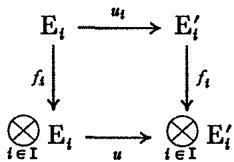
\includegraphics[keepaspectratio]{images/part003_14ac730d.jpg}}

是交换的，其中 \(f_{i}\) 和 \(f_{i}^{\prime}\) 表示典范同态。

只需将命题 8 应用于同态 \(f_{i}^{\prime} \circ u_{i}\) .

在命题 8 的推论中定义的同态 \(u\) 记作 \(\bigotimes_{i \in I} u_i\) 。若 \(J\) 是 \(I\) 的任意子集，则命题 8 可应用于典范同态族 \((f_i)_{i \in J}\) （诸 \(f_i: E_i \to \bigotimes_{i \in I} E_i = E\) ）；由此导出一个典范同态 \(E_J \to E\) ，它同样记作 \(f_J\) ，且当 \(J\) 有限时，它与上文中这样记的同态一致。

现在设 \((x_{i})_{i\in \mathbf{I}}\) 是 \(\prod_{i\in \mathbf{I}}\mathrm{E}_i\) 的一个元素，使得族 \((x_{i} - e_{i})_{i\in \mathbf{I}}\) 具有有限支撑 H。显然，若 J 和 \(J^{\prime}\) 是 I 的两个包含 H 的有限子集，则

\[
f _ {J} ((x _ {i}) _ {i \in J}) = f _ {J ^ {\prime}} ((x _ {i}) _ {i \in J ^ {\prime}}).
\]

 \(f_{\mathbf{J}}((x_i)_{i \in \mathbf{J}})\) （其中 \(\mathbf{J} \supset \mathbf{H}\) 遍历 \(\mathbf{I}\) 的有限子集）的公共值记为 \(\bigotimes_{i \in \mathbf{I}} x_i\) .

命题 9. 设 \((\mathbf{E}_i)_{i\in \mathbf{I}}\) 是一族 A-代数，且对每个 \(i\in \mathbf{I}\) ，设 \(B_{i}\) 是 \(\mathbf{E}_i\) 的一组基，使得单位元 \(e_i\) 属于 \(\overline{\mathbf{B}}_i\) 。设 \(\mathbf{B}\) 是形如 \(\bigotimes_{i\in \mathbf{I}}x_i\) 的元素组成的集合，其中 \((x_{i})\) 取遍 \(\prod_{i\in \mathbf{I}}\mathbf{B}_i\) 中使族 \((x_{i} - e_{i})\) 具有有限支撑的元素。则 \(\mathbf{B}\) 是代数 \(\bigotimes_{i\in \mathbf{I}}\mathbf{E}_i\) 的一组基，且这组基包含单位元 \(e\) .

对 I 的每个有限子集 J，设 \(B_{J}\) 是 \(E_{J} = \bigotimes_{i \in J} E_{i}\) 的基，即诸基 \(B_{i}\) （ \(i \in J\) ）的张量积（II, §3, 第 9 号）。由定义立即得出，B 是诸 \(f_{J}(B_{J})\) 当 J 遍历 \(\mathfrak{F}(I)\) 时的并，且 \(f_{J^{\prime}J}(B_{J}) \subset B_{J^{\prime}}\) 当 \(J \subset J^{\prime}\) 时成立；因此 \((B_{J})\) 是诸 \(E_{J}\) 的子集的一个正向系统，且 \(B = \varinjlim B_{J}\) ；结论由 II, §6, 第 2 号, 命题 5 的推论得出。

基 B 也称为诸基 \(B_{i}\) （ \(i \in I\) ）的张量积；当命题 9 的条件满足时，典范同态 \(f_{J}: E_{J} \to E = \bigotimes_{i \in I} E_{i}\) 对 I 的每个子集 J 都是单射，因为若 \(B_{J}\) 是 \(E_{J}\) 的基，即诸 \(B_{i}\) （ \(i \in J\) ）的张量积，则立即可以验证 \(f_{J}\) 在 \(B_{J}\) 上的限制是单射，且把 \(B_{J}\) 映到 B 的一个子集上。

\subsection{交换引理}

引理 1. 设 \(\mathbf{A}\) 是一个交换环， \(\mathbf{E}\) 是一个 \(\mathbf{A}\) -代数， \((x_{i})_{1\leqslant i\leqslant n}\) 是 \(\mathbf{E}\) 的元素组成的一个有限序列， \((\lambda_i)_{1\leqslant i\leqslant n}\) 是 \(\mathbf{A}\) 的元素组成的一个有限序列， \(y\) 是 \(\mathbf{E}\) 的一个元素；假设

\[
x _ {i} y = \lambda_ {i} y x _ {i} \quad \text { for } 1 \leqslant i \leqslant n.\tag{13}
\]

那么

\[
\left(x _ {1} x _ {2} \dots x _ {n}\right) y = \left(\lambda_ {1} \lambda_ {2} \dots \lambda_ {n}\right) y \left(x _ {1} x _ {2} \dots x _ {n}\right).\tag{14}
\]

该引理对 \(n = 1\) 是平凡的，我们对 \(n \geqslant 2\) 作归纳论证。现在

\[
\begin{array}{r l} (x _ {1} x _ {2} \dots x _ {n}) y & = (x _ {1} \dots x _ {n - 1}) (x _ {n} y) \\ & = (x _ {1} \dots x _ {n - 1}) (\lambda_ {n} y x _ {n}) = \lambda_ {n} ((x _ {1} \dots x _ {n - 1}) y) x _ {n}, \end{array}
\]

根据归纳假设，其等于

\[
\lambda_ {n} \left(\lambda_ {1} \dots \lambda_ {n - 1}\right) y \left(x _ {1} \dots x _ {n - 1}\right) x _ {n} = \left(\lambda_ {1} \dots \lambda_ {n - 1} \lambda_ {n}\right) y \left(x _ {1} \dots x _ {n - 1} x _ {n}\right),
\]

由此即得引理。

引理 2. 设 A 是一个交换环，E 是一个 A-代数， \((x_{i})_{1\leqslant i\leqslant n}\) 和 \((y_{i})_{1\leqslant i\leqslant n}\) 是 E 的由 \(n\) 个元素组成的两个有限序列；假设对 \(1\leqslant j\leqslant i\leqslant n\) ，

\[
x _ {i} y _ {j} = \lambda_ {i j} y _ {j} x _ {i} \quad \text { with } \lambda_ {i j} \in A.\tag{15}
\]

那么

\[
\left(x _ {1} x _ {2} \dots x _ {n}\right) \left(y _ {1} y _ {2} \dots y _ {n}\right) = \left(\prod_ {i > j} \lambda_ {i j}\right) \left(x _ {1} y _ {1}\right) \left(x _ {2} y _ {2}\right) \dots \left(x _ {n} y _ {n}\right).\tag{16}
\]

该引理对 \(n = 1\) 是平凡的，我们对 \(n\) （ \(n \geqslant 2\) ）再次作归纳论证。根据引理 1，

\[
\begin{array}{r l} (x _ {1} \dots x _ {n}) (y _ {1} \dots y _ {n}) & = x _ {1} (x _ {2} \dots x _ {n}) y _ {1} (y _ {2} \dots y _ {n}) \\ & = \left(\prod_ {i > 1} \lambda_ {i 1}\right) (x _ {1} y _ {1}) (x _ {2} \dots x _ {n}) (y _ {2} \dots y _ {n}) \end{array}
\]

然后只需应用归纳假设即可得到 (16)。

对元素的每个族 \(\lambda = (\lambda_{ij})\) （元素属于 A，且 \(1 \leqslant j < i \leqslant n\) ），以及对每个置换 \(\sigma \in \mathfrak{S}_n\) ，我们记

\[
\varepsilon_ {\sigma} (\lambda) = \prod_ {i > j, \sigma^ {- 1} (i) < \sigma^ {- 1} (j)} \lambda_ {i j} = \prod_ {i <   j, \sigma (i) > \sigma (j)} \lambda_ {\sigma (i), \sigma (j)}.\tag{17}
\]

注意，当 \(\mathbf{A} = \mathbf{Z}\) 且 \(\lambda_{ij} = -1\) 对每个有序对 \((i,j)\) （满足 \(1 \leqslant j < i \leqslant n\) ）成立时， \(\varepsilon_{\sigma}(\lambda)\) 就是符号 \(\varepsilon_{\sigma}\) （置换 \(\sigma\) 的符号）（I, §5, 第 7 号）。

引理 3. 设 A 是一个交换环，E 是一个 A-代数， \((x_{i})_{1\leqslant i\leqslant n}\) 是 E 的元素组成的一个有限序列，并假设对每个整数有序对 \((i,j)\) （满足 \(1\leqslant j < i\leqslant n\) ），

\[
x _ {i} x _ {j} = \lambda_ {i j} x _ {j} x _ {i} \quad \text { with } \lambda_ {i j} \in A.\tag{18}
\]

那么，对每个置换 \(\sigma \in \mathfrak{S}_n\) ，

\[
x _ {\sigma (1)} x _ {\sigma (2)} \dots x _ {\sigma (n)} = \varepsilon_ {\sigma} (\lambda) x _ {1} x _ {2} \dots x _ {n}.\tag{19}
\]

该引理对 \(n = 1\) 和 \(n = 2\) 是平凡的；我们对 \(n\) （ \(n \geqslant 3\) ）作归纳。若 \(\sigma(n) = n\) ，则关系式 (19) 由归纳假设得出。因此设 \(\sigma(n) = k, k \neq n\) ，并令 \(\tau\) 为 \([1, n]\) 上由下式定义的置换

\[
\left\{ \begin{array}{l l} \tau (i) = i & \text { for } i <   k \\ \tau (i) = i + 1 & \text { for } k \leqslant i <   n \\ \tau (n) = k. \end{array} \right.
\]

设 \(\pi = \tau^{-1} \circ \sigma\) ；置换 \(\pi\) 保持 \(n\) 不动；现在 \(\sigma = \tau \circ \pi\) ，因此，记 \(y_i = x_{\tau(i)}\) ，就有 \(y_{\pi(i)} = x_{\sigma(i)}\) 。若 \(i \neq n\) 且 \(j \neq n\) ，关系 \(\pi(i) > \pi(j)\) 与 \(\sigma(i) > \sigma(j)\) 等价（因为 \(\tau\) 是从 \([1, n - 1]\) 到 \([1, n]\) 的严格递增映射。对 \(i \neq n\) , \(j \neq n\) 和 \(\sigma(i) > \sigma(j)\) ，

\[
y _ {\pi (i)} y _ {\pi (j)} = x _ {\sigma (i)} x _ {\sigma (j)} = \lambda_ {\sigma (i), \sigma (j)} x _ {\sigma (j)} x _ {\sigma (i)} = \lambda_ {\sigma (i), \sigma (j)} y _ {\pi (j)} y _ {\pi (i)}
\]

因此，根据归纳假设（利用 \(\pi(n) = n\) ）:

\[
y _ {\pi (1)} y _ {\pi (2)} \dots y _ {\pi (n)} = \left(\prod_ {i <   j <   n, \sigma (i) > \sigma (j)} \lambda_ {\sigma (i), \sigma (j)}\right) y _ {1} y _ {2} \dots y _ {n}
\]

即

\[
x _ {\sigma (1)} x _ {\sigma (2)} \dots x _ {\sigma (n)} = \left(\prod_ {i <   j <   n, \sigma (i) > \sigma (j)} \lambda_ {\sigma (i), \sigma (j)}\right) x _ {\tau (1)} \dots x _ {\tau (n)}.\tag{20}
\]

现在

\[
x _ {\tau (1)} \dots x _ {\tau (n)} = x _ {1} \dots x _ {k - 1} x _ {k + 1} \dots x _ {n} x _ {k}
\]

而由引理 1，这等于

\[
\left(\prod_ {j > k} \lambda_ {j k}\right) x _ {1} \dots x _ {n} = \left(\prod_ {\sigma (i) > \sigma (n)} \lambda_ {\sigma (i), \sigma (n)}\right) x _ {1} \dots x _ {n}.\tag{21}
\]

最后，(20) 与 (21) 给出

\[
x _ {\sigma (1)} \dots x _ {\sigma (n)} = \alpha . x _ {1} \dots x _ {n}
\]

其中

\[
\begin{array}{l} \alpha = \left(\prod_ {i <   j <   n, \sigma (i) > \sigma (j)} \lambda_ {\sigma (i), \sigma (j)}\right) \cdot \left(\prod_ {i <   n, \sigma (i) > \sigma (n)} \lambda_ {\sigma (i), \sigma (n)}\right) \\ = \prod_ {i <   j, \sigma (i) > \sigma (j)} \lambda_ {\sigma (i), \sigma (j)} = \varepsilon_ {\sigma} (\lambda) \end{array}
\]

这就完成了引理 3 的证明。

\subsection{相对于交换因子的分次代数的张量积}

定义 6. 设 \((\Delta_{i})_{i\in I}\) 是一个以加法记号书写的交换幺半群的有限族。一个 \(\Delta_{i}\) 上的、取值于交换环 A 的交换因子系，是指一个映射系统 \(\varepsilon_{ij}:\Delta_i\times \Delta_j\to \mathbf{A}\) （其中 \(i\in \mathbf{I}, j\in \mathbf{I}, i\neq j\) ），满足以下条件：

\[
\varepsilon_ {i j} \left(\alpha_ {i} + \alpha_ {i} ^ {\prime}, \beta_ {j}\right) = \varepsilon_ {i j} \left(\alpha_ {i}, \beta_ {j}\right) \varepsilon_ {i j} \left(\alpha_ {i} ^ {\prime}, \beta_ {j}\right)\tag{22}
\]

\[
\varepsilon_ {i j} \left(\alpha_ {i}, \beta_ {j} + \beta_ {j} ^ {\prime}\right) = \varepsilon_ {i j} \left(\alpha_ {i}, \beta_ {j}\right) \varepsilon_ {i j} \left(\alpha_ {i}, \beta_ {j} ^ {\prime}\right)\tag{23}
\]

\[
\varepsilon_ {i j} (\alpha_ {i}, \beta_ {j}) \varepsilon_ {j i} (\beta_ {j}, \alpha_ {i}) = 1,\tag{24}
\]

对所有 \(\alpha_{i},\alpha_{i}^{\prime}\) （属于 \(\Delta_{i},\beta_{j},\beta_{j}^{\prime}\) ）以及 \(\Delta_j\) 中的元素成立。

若给 I 赋予一个全序且 \(\Delta_{i}\) 是群，则在 \(\Delta_{i}\) 上可以如下定义一个交换因子系：对每个有序对 \((i,j)\) （满足 i\textless j ），任取一个从 \(\Delta_{i}\times\Delta_{j}\) 到由环 A 的可逆元素组成的（乘法）Z-模 A* 的 Z-双线性映射，然后写出

\[
\varepsilon_ {j i} (\beta_ {j}, \alpha_ {i}) = (\varepsilon_ {i j} (\alpha_ {i}, \beta_ {j})) ^ {- 1}
\]

对 \(i < j\) .

注意，由于 \(\varepsilon_{ij}(\alpha_{i},\beta_{j})\) 都是可逆的，

\[
\varepsilon_ {i j} (0, \beta_ {j}) = \varepsilon_ {i j} (\alpha_ {i}, 0) = 1,
\]

由 (22) 与 (23) 即得。

例。(1) 平凡的交换因子系由满足下列条件的 \(\varepsilon_{ij}\) 组成： \(\varepsilon_{ij}(\alpha_i, \beta_j) = 1\) 对所有 \(i, j, \alpha_i \in \Delta_i, \beta_j \in \Delta_j\) 成立.

\begin{enumerate}
\def\labelenumi{(\arabic{enumi})}
\setcounter{enumi}{1}
\tightlist
\item
  若取 \(\mathbf{A} = \mathbf{Z}\) 且取 \(\Delta_{i} = \mathbf{Z}\) （对所有 \(i \in \mathbf{I}\) ），则令 \(\varepsilon_{ij}(\alpha_i, \beta_j) = (-1)^{\alpha_i\beta_j}\) 即得到一个交换因子系。注意，这个数仅依赖于 \(\alpha_{i}\) 和 \(\beta_{j}\) 的奇偶性，因此 \(\varepsilon_{ij}\) 在某些 \(\Delta_{i}\) 等于 \(\mathbf{Z}/2\mathbf{Z}\) 而其余的等于 \(\mathbf{Z}\) 的情形下仍可作为交换因子。
\end{enumerate}

这两个例子是应用中最常见的情况。

命题 10. 设 A 是一个交换环， \((\Delta_{i})_{i\in I}\) 是一个以加法记号书写的交换幺半群的有限族；对每个 \(i\in I\) ，设 \(\mathbf{E}_i\) 是一个类型为 \(\Delta_i\) 的分次 A-代数。最后，设 \((\varepsilon_{ij})\) 是 \(\Delta_i\) 上的一个取值于 A 的交换因子系。则存在一个类型为 \(\Delta = \prod_{i\in I}\Delta_i\) 的分次 A-代数 E，以及对每个 \(i\in I\) 的一个代数同态 \(h_i:\mathbf{E}_i\to \mathbf{E}\) ，具有下列性质：

\begin{enumerate}
\def\labelenumi{(\roman{enumi})}
\item
  若 \(\phi_{i}:\Delta_{i}\to\Delta\) 是典范同态，则 \(h_{i}\) 是分次同态（II, § 11, 第 2 号），换言之， \(h_{i}(E_{i}^{\alpha_{i}})\subset E^{\phi_{i}(\alpha_{i})}\) ，其中 \((E_{i}^{\alpha_{i}})\) 与 \((E^{\alpha})\) 分别表示 \(E_{i}\) 与 \(E\) 上的分次。
\item
  若 \(i \neq j\) 且 \(x_{i}\) （相应地 \(x_{j}\) ）是 \(\mathbf{E}_i\) （相应地 \(\mathbf{E}_j\) ）的次数为 \(\alpha_i \in \Delta_i\) （相应地 \(\beta_j \in \Delta_j\) ）的齐次元素，则
\end{enumerate}

\[
h _ {i} (x _ {i}) h _ {j} (x _ {j}) = \varepsilon_ {i j} (\alpha_ {i}, \beta_ {j}) h _ {j} (x _ {j}) h _ {i} (x _ {i}).\tag{25}
\]

\begin{enumerate}
\def\labelenumi{(\roman{enumi})}
\setcounter{enumi}{2}
\tightlist
\item
  对每个 A-代数 \(\mathbf{F}\) 以及每个满足下列条件的同态系统 \(f_{i}:\mathbf{E}_{i}\to \mathbf{F}\)
\end{enumerate}

\[
f _ {i} (x _ {i}) f _ {j} (x _ {j}) = \varepsilon_ {i j} (\alpha_ {i}, \beta_ {j}) f _ {j} (x _ {j}) f _ {i} (x _ {i}),\tag{26}
\]

其中 \(i, j, x_i, x_j, \alpha_i, \beta_j\) 如 (ii) 中所述，则存在且仅存在一个代数同态 \(f: \mathbf{E} \to \mathbf{F}\) ，使得 \(f_i = f \circ h_i\) 对所有 \(i \in \mathbf{I}\) 成立。此外， \(\mathbf{E}\) 的底 A-模是张量积 \(\bigotimes_{i \in \mathbf{I}} \mathbf{E}_i\) .

考虑 A-模 \(E = \bigotimes_{i \in I} E_i\) ；它等同于子模 \(E^\alpha\) 的直和，其中对每个 \(\alpha = (\alpha_i) \in \Delta\) ，记 \(E^\alpha = \bigotimes_{i \in I} E_i^{\alpha_i}\) ；因而这些 \(E^\alpha\) 在 A-模 E 上构成一个类型为 \(\Delta\) 的分次。我们将要在 E 上定义一个类型为 \(\Delta\) 的分次 A-代数结构。为此，给 I 一个全序；对每一对元素 \(\alpha = (\alpha_i)\) , \(\beta = (\beta_i)\) （属于 \(\Delta\) ），我们必须首先定义一个从 \(E^\alpha \times E^\beta\) 到 \(E^\alpha + \beta\) 的 A-双线性映射，或者等价地，定义一个 A-线性映射 \(m_{\alpha\beta}\) ，它把 \(E^\alpha \otimes_A E^\beta\) 映到 \(E^\alpha + \beta\) 。我们将用条件来定义 \(m_{\alpha\beta}\)

\[
m _ {\alpha \beta} \left(\left(\bigotimes_ {i \in I} x _ {i}\right) \otimes \left(\bigotimes_ {i \in I} y _ {i}\right)\right) = \varepsilon (\alpha , \beta) \bigotimes_ {i \in I} (x _ {i} y _ {i})\tag{27}
\]

对于 \(x_{i}\in \mathrm{E}_{i}^{\alpha_{i}},y_{i}\in \mathrm{E}_{i}^{\beta_{i}}\) ，其中

\[
\varepsilon (\alpha , \beta) = \prod_ {i > j} \varepsilon_ {i j} (\alpha_ {i}, \beta_ {j}).\tag{28}
\]

(27) 的右边显然属于 \(\mathbf{E}^{\alpha +\beta}\) ，且映射 \((x_{1},\ldots ,x_{n},y_{1},\ldots ,y_{n})\mapsto \varepsilon (\alpha ,\beta)\bigotimes_{i\in I}(x_{i}y_{i})\) 在诸 \(\mathrm{E}_i^{\alpha_i}\) 与诸 \(\mathrm{E}_i^{\beta_i}(1\leqslant i\leqslant n)\) 的乘积中是 A-多重线性的。接着必须证明这样定义在 E 上的乘法是结合的；现在，若 \(\gamma = (\gamma_{i})\) 是 \(\Delta\) 的第三个元素，且 \(z_{i} \in \mathrm{E}_{i}^{\gamma_{i}}\) （对 \(1 \leqslant i \leqslant n\) ），则

\[
\left(\left(\bigotimes_ {i} x _ {i}\right) \left(\bigotimes_ {i} y _ {i}\right)\right) \left(\bigotimes_ {i} z _ {i}\right) = \varepsilon (\alpha + \beta , \gamma) \varepsilon (\alpha , \beta) \bigotimes_ {i} (x _ {i} y _ {i} z _ {i})
\]

\[
\left(\bigotimes_ {i} x _ {i}\right) \left(\left(\bigotimes_ {i} y _ {i}\right) \left(\bigotimes_ {i} z _ {i}\right)\right) = \varepsilon (\alpha , \beta + \gamma) \varepsilon (\beta , \gamma) \bigotimes_ {i} (x _ {i} y _ {i} z _ {i})
\]

从而只需验证恒等式

\[
\varepsilon (\alpha + \beta , \gamma) \varepsilon (\alpha , \beta) = \varepsilon (\alpha , \beta + \gamma) \varepsilon (\beta , \gamma).
\]

但后者立即由以下关系得出

\[
\varepsilon (\alpha + \beta , \gamma) = \varepsilon (\alpha , \beta) \varepsilon (\beta , \gamma)
\]

\[
\varepsilon (\alpha , \beta + \gamma) = \varepsilon (\alpha , \beta) \varepsilon (\alpha , \gamma)
\]

这些关系本身是定义(28)、(22)和(23)的直接推论。

若对所有 \(i \in \mathbf{I}\) ， \(e_i\) 表示 \(\mathbf{E}_i\) 的单位元，我们知道 \(e_i\) 是 0 次齐次的（§ 3, 第 1 号），因此 \(e = \bigotimes_{i \in \mathbf{I}} e_i\) 是 0 次齐次的，并且由 (27)、(28) 及关系式

\[
\varepsilon_ {i j} (\alpha_ {i}, 0) = \varepsilon_ {i j} (0, \beta_ {j}) = 1
\]

即 \(e\) 是 \(\mathbf{E}\) 的单位元，这就完成了 \(\mathbf{E}\) 上所需要的分次 A-代数结构的定义。然后取 \(h_i(x_i) = x_i \otimes \bigotimes_{j \neq i} e_j\) ；为验证 \(h_i(x_i x_i') = h_i(x_i) h_i(x_i')\) 对 \(x_i, x_i'\) （属于 \(\mathbf{E}_i\) ）成立，只需限于 \(x_i\) 和 \(x_i'\) 均为齐次元素的情形，此时该关系由 (27) 和关系式 \(\varepsilon_{ij}(\alpha_i, 0) = \varepsilon_{ij}(0, \beta_j) = 1\) 立即得出；同样的关系式以及 (24) 还证明了 \(h_i\) 满足命题中的条件 (i) 与 (ii)，且

\[
\bigotimes_ {i \in I} x _ {i} = \prod_ {i \in I} h _ {i} (x _ {i})\tag{29}
\]

其中右端是有序序列 \((h_i(x_i))_{i\in I}\) 按 I 上给定的全序在 E 中取的乘积（I, § 1, 第 2 号）（只需对 \(x_{i}\) （设为齐次）中异于 \(e_i\) 者的个数作归纳论证即可）.

仍需证明条件 (iii)；注意，映射

\[
(x _ {i}) _ {i \in I} \mapsto \prod_ {i \in I} f _ {i} (x _ {i}),
\]

其中右端是有序序列 \((f_{i}(x_{i}))_{i\in\mathbf{I}}\) 按 I 上给定的全序取的乘积，是 A-多重线性的。于是存在且仅存在一个 A-线性映射 \(f: E \rightarrow F\) ，使得

\[
f \left(\bigotimes_ {i \in I} x _ {i}\right) = \prod_ {i \in I} f _ {i} (x _ {i}).\tag{30}
\]

显然 \(f(e)\) 是 \(\mathbf{F}\) 的单位元，且 \(f \circ h_i = f_i\) ；为验证 \(f\) 是代数同态，换言之，验证 \(f(x)f(y) = f(xy)\) 对 \(x, y\) （属于 \(\mathbf{E}\) ）成立，由线性性，只需限于下列情形： \(x = \bigotimes_{i \in \mathbf{I}} x_i\) 且 \(y = \bigotimes_{i \in \mathbf{I}} y_i\) ，其中 \(x_i\) （相应地 \(y_i\) ）是次数为 \(\alpha_i\) （相应地 \(\beta_i\) ）的齐次元素（对所有 \(i \in \mathbf{I}\) ）。此时，要验证的关系式由 (27) 化归为

\[
\left(\prod_ {i \in \mathrm{I}} f _ {i} (x _ {i})\right) \left(\prod_ {i \in \mathrm{I}} f _ {i} (y _ {i})\right) = \varepsilon (\alpha , \beta) \prod_ {i \in \mathrm{I}} \left(f _ {i} (x _ {i}) f _ {i} (y _ {i})\right).
\]

但考虑到关系式 (26)，这是第 6 号的引理 2 的一个推论。

显然，代数 E 与典范映射 \(\psi: \bigotimes_{i \in I} E_i \to E\) 构成泛映射问题（集合论, IV, § 3, 第 1 号）的一个解，其中 \(\Sigma\) 是 A-代数结构的种类，而 \(\alpha\) -映射是映射 \(\prod_{i} f_i\) （从 \(\prod_{i} E_i\) 到一个 A-代数，满足条件 (26)）。

对 I 上固定的一个全序，命题 10 的证明中所定义的分次代数 E 将称为一个分次张量 \(\varepsilon\) -积，其类型为 \(\Delta\) ，所属的族为 \((\mathrm{E}_i)_{i\in \mathbf{I}}\) （族中各代数的类型为 \(\Delta_i\) ），并记作 \({}^{\varepsilon}\bigotimes_{i\in \mathbf{I}}\mathrm{E}_i\) （若关于 I 上的序不致引起混淆）；类似地，命题 10 的证明中定义的同态 \(f:\mathrm{E}\to \mathrm{F}\) 将记作 \({}^{\varepsilon}\bigotimes_{i\in \mathbf{I}}f_i\) 。同态 \(h_i\) 称为典范的。我们也写作 \({}^{\varepsilon}\mathrm{G}^{\otimes n}\) （当 \(\mathbf{I} = [1,n]\) 且所有 \(\mathrm{E}_i\) 都等于同一个代数 G 时）。

注。(1) 若取 \(\varepsilon_{ij}(\alpha_i, \beta_j) = 1\) （对所有 \(i, j, \alpha_i\) 与 \(\beta_j\) ），我们就重新得到第 1 号中定义的代数的张量积（其分次还是各因子的分次的张量积）.

\begin{enumerate}
\def\labelenumi{(\arabic{enumi})}
\setcounter{enumi}{1}
\tightlist
\item
  设所有 \(\Delta_{i}\) 都等于 \(\mathbf{Z}\) ，并写 \(\varepsilon_{ij}(\alpha_i, \beta_j) = (-1)^{\alpha_i \beta_j}\) ；对应于这个交换因子系的张量 \(\varepsilon\) -积 \({}^{\varepsilon}\bigotimes_{i \in I} E_i\) 称为分次代数 \(E_i\) （类型为 \(\mathbf{Z}\) ）的斜张量积，记作 \({}^{g}\bigotimes_{i \in I} E_i\) （对两个代数则记 \(E{}^{g} \otimes_A F\) ，或以 \({}^{g} G^{\otimes n}\) 代替 \({}^{\varepsilon} G^{\otimes n}\) ）.
\end{enumerate}

推论 1. 在命题 10 的记号下，进一步设 F 是一个类型为 \(\Delta\) 的分次 A-代数，且每个 \(f_{i}\) 都是相对于 \(\phi_{i}:\Delta_{i}\to\Delta\) 的分次代数同态；则 \(f={}^{\varepsilon}\bigotimes_{i}f_{i}\) 是一个分次代数同态。

这由 \(f\) 的定义以及下列事实立即得出：

\[
\sum_ {i \in I} \phi_ {i} (\alpha_ {i}) = (\alpha_ {i})
\]

这是由 \(\phi_{i}\) 的定义得到的.

由此可以看出， \((\mathrm{E},\psi)\) 也是另一个泛映射问题的解，这一次 \(\Sigma\) 是类型为 \(\Delta\) 的分次 A-代数结构的种类，其态射是类型为 \(\Delta\) 的分次代数同态，而 \(\alpha\) -映射是映射 \(\prod_{i}f_{i}\) （其中除条件 (26) 外，还假设 \(f_{i}\) 是相对于 \(\phi_{i}\) 的分次代数同态）.

推论 2. 设 \((\mathbf{E}_i)_{i\in \mathbf{I}}\) , \((\mathbf{F}_i)_{i\in \mathbf{I}}\) 是两个有限的 A-代数族，且 \(\mathbf{E}_i\) 与 \(\mathbf{F}_i\) 都是类型为 \(\Delta_i\) 的分次代数（对所有 \(i\in \mathbf{I}\) ）。对每个 \(i\in \mathbf{I}\) ，设 \(g_i:\mathbf{E}_i\to \mathbf{F}_i\) 是一个类型为 \(\Delta_i\) 的分次代数同态。那么，若 \(h_i:\mathbf{E}_i\to {}^{\varepsilon}\bigotimes_{i\in \mathbf{I}}\mathbf{E}_i\) 与 \(h_i':\mathbf{F}_i\to {}^{\varepsilon}\bigotimes_{i\in \mathbf{I}}\mathbf{F}_i\) 是典范同态，则存在且仅存在一个类型为 \(\Delta\) 的分次 A-代数同态 \(g: {}^{\varepsilon}\bigotimes_{i\in \mathbf{I}}\mathbf{E}_i\to {}^{\varepsilon}\bigotimes_{i\in \mathbf{I}}\mathbf{F}_i\) ，使得 \(g\circ h_i = h_i'\circ g_i\) 对所有 \(i\in \mathbf{I}\) 成立。此外，若每个 \(g_i\) 都是双射，则 \(g\) 也是.

只需将推论 1 应用于 \(f_{i} = h_{i}^{\prime} \circ g_{i}\) ，并注意到条件 (26) 可由应用于 \(h_{i}^{\prime}\) 的关系式 (25) 得出。

推论 2 中定义的同态也记作 \({}^{\varepsilon}\bigotimes_{i} g_{i}\) （若不致引起混淆）；若对每个 \(i \in I\) ， \(G_{i}\) 是又一个分次 A-代数（类型为 \(\Delta_{i}\) ），且 \(g_{i}^{\prime}: F_{i} \to G_{i}\) 是一个分次代数同态，则

\[
\left(^ {\varepsilon} \bigotimes_ {i} g _ {i} ^ {\prime}\right) \circ \left(^ {\varepsilon} \bigotimes_ {i} g _ {i}\right) = ^ {\varepsilon} \bigotimes_ {i} \left(g _ {i} ^ {\prime} \circ g _ {i}\right),\tag{31}
\]

这由(30)立即得出。

在斜张量积（类型为 \(\mathbf{Z}\) 的分次代数的）情形，我们写 \({}^{g}\bigotimes_{i}f_{i}\) 以代替 \({}^{\varepsilon}\bigotimes_{i}f_{i}\) ——对同态 \(f_{i}: \mathrm{E}_{i} \to \mathrm{F}_{i}\) （类型为 \(\mathbf{Z}\) 的分次代数的同态）而言；当 \(\mathrm{I} = \{1, 2\}\) 时，这个同态也记作 \(f_{1}{}^{g}\otimes f_{2}\) ；当 \(\mathrm{I} = [1, n]\) 且所有 \(\mathrm{E}_{i}\) （相应地 \(\mathrm{F}_{i}\) ）相等并且所有 \(f_{i}\) 都等于同一个同态 \(f\) 时，我们写 \({}^{g}f^{\otimes n}\) .

注。在命题 10 的证明中，I 上的一个全序被用来在张量积 \(\bigotimes_{i\in I}E_i\) 上定义一个代数结构，该张量积是 A-模

\(E_{i}\) 的张量积。若改变 I 上的序，则在 \(\bigotimes_{i\in I}E_{i}\) 上会产生另一个乘法结构，但这样得到的新代数与上述代数典范同构，因为二者都是同一个泛映射问题的解。例如，当 \(I=\{1,2\}\) 时，从代数 \(E_{1}{}^{\varepsilon}\otimes_{A}E_{2}\) 到代数 \(E_{2}{}^{\varepsilon}\otimes_{A}E_{1}\) 的典范同构把 \(x_{1}\otimes x_{2}\) 映为 \(\varepsilon_{2,1}(\alpha,\beta)x_{2}\otimes x_{1}\) ，其中 \(x_{1}\) 是次数为 \(\alpha\) 的齐次元素， \(x_{2}\) 是次数为 \(\beta\) 的齐次元素.

设 J 是 I 的一个子集，且对每个 \(i \in J\) ，考虑典范同态 \(h_{i}: E_{i} \to {}^{\varepsilon}\bigotimes_{i \in I} E_{i} = E\) 。借助关系式 (25)，从这些同态典范地（由命题 10）导出一个典范同态 \(h: E' = {}^{\varepsilon}\bigotimes_{i \in J} E_{i} \to E\) ，使得对所有 \(i \in J\) ， \(h_{i}' = h \circ h_{i}\) ，其中 \(h_{i}'\) 是典范同态 \(E_{i} \to E'\) 。取 J 上由 I 上所选的全序诱导的全序，我们得到

\[
h \left(\bigotimes_ {i \in J} x _ {i}\right) = \prod_ {i \in I} h _ {i} \left(x _ {i}\right) = \bigotimes_ {i \in I} x _ {i} ^ {\prime}
\]

其中中间项是有序序列 \((h_i(x_i))_{i\in J}\) 的乘积，而在右端项中， \(x_{i}^{\prime} = x_{i}\) 对 \(i\in J\) 成立， \(x_{i}^{\prime} = e_{i}\) 对 \(i\notin J\) 成立.

命题 11.（张量 \(\varepsilon\) -积的“结合性”）。在命题 10 的记号下，设 \((J_{\lambda})_{\lambda \in L}\) 是 I 的一个划分，并记 \(\Delta_{\lambda}' = \prod_{i \in J_{\lambda}} \Delta_i\) （对所有 \(\lambda \in L\) ）。设 \(E_{\lambda}'\) 是一个分次张量 \(\varepsilon\) -积，其类型为 \(\Delta_{\lambda}'\) ，所属的族为 \((E_i)_{i \in J_{\lambda}}\) （对 \(J_{\lambda}\) 上选定的某个全序而言）。另一方面，对 L 中的 \(\lambda, \mu\) 且 \(\lambda \neq \mu\) ，我们对 \(\alpha_{\lambda}' = (\alpha_i)_{i \in J_{\lambda}}, \beta_{\mu}' = (\beta_j)_{j \in J_{\mu}}\) 写

\[
\varepsilon_ {\lambda \mu} ^ {\prime} (\alpha _ {\lambda} ^ {\prime}, \beta_ {\mu} ^ {\prime}) = \prod_ {i \in J _ {\lambda}, j \in J _ {\mu}} \varepsilon_ {i j} (\alpha_ {i}, \beta_ {j}).\tag{32}
\]

那么 \((\varepsilon_{\lambda \mu}^{\prime})\) 是 \(\Delta_{\lambda}^{\prime}\) 上的一个取值于 A 的交换因子系，且存在且仅存在一个类型为 \(\Delta, v: {}^{\varepsilon'}\bigotimes_{\lambda \in L} E_{\lambda}^{\prime} \to {}^{\varepsilon}\bigotimes_{i \in I} E_{i}\) 的分次代数同态，使得

\[
v \left(\bigotimes_ {\lambda \in L} \left(\bigotimes_ {i \in J _ {\lambda}} x _ {i}\right)\right) = \bigotimes_ {i \in I} x _ {i}\tag{33}
\]

对所有 \((x_{i})\in \prod_{i\in \mathbf{I}}\mathrm{E}_{i}\) 成立，前提是在 \(\mathbf{I}\) 上取这样的全序：它在每个 \(\mathbf{J}_{\lambda}\) 上诱导所选的全序，并且使得对 \(\lambda < \mu\) （在 \(\mathbf{L}\) 中）、 \(i\in \mathbf{J}_{\lambda}\) 与 \(j\in \mathbf{J}_{\mu}\) ，有 \(i < j\) .

\(\varepsilon_{\lambda \mu}'\) 构成交换因子系这一事实是平凡的。设 \(h_{i,\lambda}:\mathrm{E}_i\to \mathrm{E}_{\lambda}', h_{\lambda}':\mathrm{E}_{\lambda}'\to {}^{\varepsilon'}\bigotimes_{\lambda \in L}\mathrm{E}_{\lambda}'\) 是典范同态（对 \(\lambda \in L\) , \(i\in \mathbf{J}_{\lambda}\) ），并记 \(h_i'' = h_\lambda' \circ h_{i,\lambda}\) ；由泛映射问题解的唯一性，只需证明 \({}^{\varepsilon'}\bigotimes_{\lambda \in L} E_{\lambda}'\) 与诸 \(h_i''\) 满足命题 10 的条件即可。现在，对所有 \(\lambda \in L\) ，设 \(f_{\lambda}': E_{\lambda}' \to F\) 是唯一的代数同态，使得 \(f_{\lambda}' \circ h_{i,\lambda} = f_i\) 对所有 \(i \in J_{\lambda}\) 成立。我们证明，对 \(\lambda \neq \mu\) , \(\alpha_{\lambda}' = (\alpha_i)_{i \in J_{\lambda}}\) , \(\beta_{\mu}' = (\beta_j)_{j \in J_{\mu}}\) ,

\[
f _ {\lambda} ^ {\prime} (x _ {\lambda} ^ {\prime}) f _ {\mu} ^ {\prime} (x _ {\mu} ^ {\prime}) = \varepsilon_ {\lambda \mu} ^ {\prime} (\alpha_ {\lambda} ^ {\prime}, \beta_ {\mu} ^ {\prime}) f _ {\mu} ^ {\prime} (x _ {\mu} ^ {\prime}) f _ {\lambda} ^ {\prime} (x _ {\lambda} ^ {\prime})\tag{34}
\]

对齐次元素 \(x_{\lambda}^{\prime} \in \mathrm{E}_{\lambda}^{\prime}\) （相应地 \(x_{\mu}^{\prime} \in \mathrm{E}_{\mu}^{\prime}\) ），其次数为 \(\alpha_{\lambda}^{\prime}\) （相应地 \(\beta_{\mu}^{\prime}\) ）；由线性性，只需在 \(x_{\lambda}^{\prime} = \bigotimes_{i \in J_{\lambda}} x_{i}\) , \(x_{\mu}^{\prime} = \bigotimes_{j \in J_{\mu}} x_{j}\) 的情形验证，其中 \(x_{i}\) （相应地 \(x_{j}\) ）是次数为 \(\alpha_{i}\) （相应地 \(\beta_{j}\) ）的齐次元素，属于 \(E_{i}\) （相应地 \(E_{j}\) ）（对 \(i \in J_{\lambda}, j \in J_{\mu}\) ）。但这由定义诸 \(f_{\lambda}^{\prime}\) 的公式 (30) 以及第 6 号的引理 3 得出，其中用到假设 (26) 与定义 (32)。因此存在且仅存在一个代数同态 \(f: ^{\varepsilon'} \bigotimes_{\lambda \in L} E_{\lambda}' \to F\) ，使得 \(f \circ h_{\lambda}' = f_{\lambda}'\) 对所有 \(\lambda \in L\) 成立；由此 \(f \circ h_{i}' = f_{i}\) 对所有 \(i \in I\) 成立，而 \(f\) 的唯一性是平凡的。

\subsection{同类型分次代数的张量积}

在第 7 号命题 10 的假设成立的前提下，进一步设所有 \(\Delta_{i}\) 都等于同一个交换幺半群 \(\Delta_{0}\) ；于是我们可以在张量 \(\varepsilon\) -积 \({}^{\varepsilon}\bigotimes_{i\in I}E_{i}\) 上考虑类型为 \(\Delta_{0}\) 的总分次，它与此代数上类型为 \(\Delta = \Delta_{0}^{I}\) 的分次相关联（II, § 11, 第 1 号）；我们将带有这个分次的 \({}^{\varepsilon}\bigotimes_{i\in I}E_{i}\) 称为一个分次张量 \(\varepsilon\) -积，其类型为 \(\Delta_{0}\) ，所属的族为 \((E_{i})_{i\in I}\) （族中各代数的类型为 \(\Delta_{0}\) ）.

保持第 7 号命题 10 的记号，设 F 也是一个类型为 \(\Delta_0\) 的分次 A-代数，且诸 \(f_i\) 是类型为 \(\Delta_0\) 的分次代数同态。则 \(f: {}^{\varepsilon}\bigotimes_{i \in I} E_i \to F\) 也是类型为 \(\Delta_0\) 的分次代数同态：因为由公式 (30)（第 7 号）可知，若 \(x_i\) 是齐次的且次数为 \(\alpha_i \in \Delta_0\) ，则 \(\bigotimes_{i \in I} x_i\) 与 \(\prod_{i \in I} f_i(x_i)\) 都是次数为 \(\sum_{i \in I} \alpha_i \in \Delta_0\) 的齐次元素.

因此可以说， \(\bigotimes_{i\in I}E_i\) （带有类型为 \(\Delta_0\) 的总分次）与典范映射 \(\psi\) 一起构成第三个泛映射问题的一个解，其中 \(\Sigma\) 是类型为 \(\Delta_0\) 的分次 A-代数的种类，态射是类型为 \(\Delta_0\) 的分次代数同态，而 \(\alpha\) -映射是映射 \(\prod_{i}f_{i}\) （其中除条件 (26)（第 7 号）外，还假设每个 \(f_{i}\) 是类型为 \(\Delta_0\) 的分次代数同态）.

对 I 的每个子集 J，典范同态 \({}^{\varepsilon}\bigotimes_{i\in J}E_i\to {}^{\varepsilon}\bigotimes_{i\in I}E_i\) （第 7 号）实际上是一个类型为 \(\Delta_0\) 的分次代数同态，这由上述内容立即得出。

命题 12.（同类型分次代数的张量 \(\varepsilon\) -积的“结合性”）。采用第 7 号命题 10 的记号，设所有 \(\Delta_{i}\) 都等于同一个幺半群 \(\Delta_{0}\) ；设 \((J_{\lambda})_{\lambda \in L}\) 是 I 的一个划分。采用第 7 号命题 11 的记号，设公式 (32)（第 7 号）的右端只依赖于和 \(\alpha_{\lambda}^{\prime \prime} = \sum_{i \in J_{\lambda}} \alpha_{i}, \beta_{\mu}^{\prime \prime} = \sum_{j \in J_{\mu}} \beta_{j}\) ——对相异指标的每个有序对 \((\lambda, \mu)\) 、所有 \(\alpha_{\lambda}^{\prime} \in \Delta_{\lambda}^{\prime}\) 以及所有 \(\beta_{\mu}^{\prime} \in \Delta_{\mu}^{\prime}\) 而言；令 \(\varepsilon_{\lambda \mu}^{\prime \prime}(\alpha_{\lambda}^{\prime \prime}, \beta_{\mu}^{\prime \prime})\) 表示 (32) 的右端。则 \((\varepsilon_{\lambda \mu}^{\prime \prime})\) 是族 \((\Delta_{\lambda}^{\prime \prime})_{\lambda \in L}\) 上的一个交换因子系，其中 \(\Delta_{\lambda}^{\prime \prime} = \Delta_{0}\) （对所有 \(\lambda \in L\) ）。若 \(E_{\lambda}^{\prime \prime}\) 是一个分次张量 \(\varepsilon\) -积，其类型为 \(\Delta_{0}\) ，所属的族为 \((E_{i})_{i \in J_{\lambda}}\) ，则存在且仅存在一个类型为 \(\Delta_{0}\) 的分次代数同构 \(w: {}^{\varepsilon}\bigotimes_{\lambda \in L} E_{\lambda}^{\prime \prime} \to {}^{\varepsilon}\bigotimes_{i \in I} E_{i}\) ，使得

\[
w \left(\bigotimes_ {\lambda \in L} \left(\bigotimes_ {i \in J _ {\lambda}} x _ {i}\right)\right) = \bigotimes_ {i \in I} x _ {i}\tag{35}
\]

前提是按第 7 号命题 11 所述，在 \(\mathbf{J}_{\lambda}\) 与 \(\mathbf{I}\) 上选取全序。

根据假设，对 \(\gamma\) , \(\delta\) （属于 \(\Delta_0\) ），有 \(\varepsilon_{\lambda \mu}''(\gamma, \delta) = \varepsilon_{i_0 j_0}(\gamma, \delta)\) （对某个 \(i_0 \in J_\lambda\) 与某个 \(j_0 \in J_\mu\) ），这可以通过考虑元素 \(\alpha_\lambda' = (\alpha_i)_{i \in J_\lambda}\) 与 \(\beta_\mu' = (\beta_j)_{j \in J_\mu}\) 看出，它们满足 \(\alpha_{i_0} = \gamma\) , \(\alpha_i = 0\) （对 \(i \neq i_0\) ）, \(\beta_{j_0} = \delta\) , \(\beta_j = 0\) （对 \(j \neq j_0\) ）；由此立即得出，诸 \(\varepsilon_{\lambda \mu}''\) 构成一个交换因子系。证明的其余部分与命题 11（第 7 号）的证明类似，留给读者完成。

注意，当 \(\Delta_0 = \mathbf{Z}\) 且 \((\varepsilon_{ij})\) 是平凡的因子系 \((\varepsilon_{ij}(\alpha_i,\beta_j) = 1\) 对所有 \(i,j)\) ，或是由 \(\varepsilon_{ij}(\alpha_i,\beta_j) = (-1)^{\alpha_i\beta_j}\) 定义的因子系时，命题 12 的附加假设成立；在后一情形，公式 (32) 的右端等于 \((-1)^{\gamma}\) ，其中 \(\gamma = \sum_{i\in J_{\lambda},j\in J_{\mu}}\alpha_{i}\beta_{j} = \left(\sum_{i\in J_{\lambda}}\alpha_{i}\right)\left(\sum_{j\in J_{\mu}}\beta_{j}\right)\) .

注。(1) 设 I 是一个无限指标集， \(\Delta_0\) 是一个交换幺半群；设 \((\Delta_i)_{i \in I}\) 表示满足 \(\Delta_i = \Delta_0\) （对所有 \(i\) ）的族，并对 I 的每对相异指标 \((i,j)\) 给定一个满足条件 (22)、(23) 与 (24)（第 7 号）的映射 \(\varepsilon_{ij} : \Delta_i \times \Delta_j \to A\) ；这也称为族 \((\Delta_i)\) 上的一个交换因子系。考虑一个族 \((E_i)_{i \in I}\) （由类型为 \(\Delta_0\) 的分次 A-代数组成）；对 I 的每个有限子集 J，令 \(E_J\) 表示一个分次张量 \(\varepsilon\) -积，其类型为 \(\Delta_0\) ，所属的子族为 \((E_i)_{i \in J}\) （对 J 上的全序作任意选取）。若 J 与 \(J'\) 是 I 的两个有限子集且 \(J \subset J'\) ，则上面已定义了一个类型为 \(\Delta_0\) 的分次代数的典范同态 \(h_{J^{\prime}J}:E_{J}\to E_{J^{\prime}}\) ，而这些同态的唯一性性质立即表明：若 \(J\subset J^{\prime}\subset J^{\prime\prime}\) 是 I 的三个有限子集，则 \(h_{J^{\prime\prime}J}=h_{J^{\prime\prime}J^{\prime}}\circ h_{J^{\prime}J}\) 。于是有一个正向系统 \((E_{J},h_{J^{\prime}J})\) ——由类型为 \(\Delta_{0}\) 的分次代数组成（§3, 第 3 号）——其指标集是 I 的有限子集组成的右有向集 \(\mathfrak{F}(I)\) 。类型为 \(\Delta_{0}\) 的分次代数——这个正向系统的正向极限（§3, 第 3 号）——称为一个分次张量 \(\varepsilon\) -积，其类型为 \(\Delta_{0}\) ，所属的族为 \((E_{i})_{i\in I}\) ；它也记作 \({}^{\varepsilon}\bigotimes_{i\in I}E_{i}\) 。当所有 \(\Delta_{i}\) 都等于 \(\mathbf{Z}\) 且 \(\varepsilon_{ij}(\alpha_{i},\beta_{j})=(-1)^{\alpha_{i}\beta_{j}}\) 时，张量积 \({}^{\varepsilon}\bigotimes_{i\in I}E_{i}\) 也称为

族 \((\mathbf{E}_{i})_{i\in\mathbb{I}}\) 的斜张量积，记作 \({}^{g}\bigotimes_{i\in I}E_{i}\) 。我们把如下命题的表述与证明留给读者：该命题把第 7 号的命题 10 推广到 I 为无限的情形，正如第 5 号的命题 8 把第 2 号的命题 5 推广到 I 为无限的情形那样。注意， \({}^{\varepsilon}\bigotimes_{i\in I}E_{i}\) 的底 A-模与第 5 号中定义的非分次代数的族 \((\mathbf{E}_{i})_{i\in\mathbb{I}}\) 的（非分次）张量积的底 A-模相同。

\begin{enumerate}
\def\labelenumi{(\arabic{enumi})}
\setcounter{enumi}{1}
\tightlist
\item
  设 E 是一个类型为 \(\Delta_0\) 的分次 A-代数（其中 \(\Delta_0\) 是一个交换幺半群），且 \(\rho: \mathbf{A} \to \mathbf{B}\) 是一个环同态； \(\rho^*(\mathbf{E})\) 上的分次（II, §11, 第 5 号）与分次张量积 \(\mathbf{B} \otimes_{\mathbf{A}} \mathbf{E}\) （其中 B 带有平凡分次）上的分次相同。
\end{enumerate}
% semantic-fragments: legacy-input-seam
\relax{}
\subsection{反交换代数与交错代数}

定义7. 一个Z型分次A-代数E称为反交换的，如果对所有非零齐次元素x，y\ensuremath{\in}E

\[
x y = (- 1) ^ {\deg (x) \deg (y)} y x.\tag{36}
\]

代数 \(\mathbf{E}\) 称为交错的，如果它是反交换的，并且还满足 \(x^{2} = 0\) （对每个奇次数的齐次元素 \(x\in \mathbf{E}\) ）。

注记. (1) 设 \(\mathbf{E}^{+}\) 为 \(\mathbf{E}\) 的分次子代数，即诸 \(\mathrm{E}_{2n}\) ( \(n \in \mathbf{Z}\) ) 的直和；由定义7可知，若 \(\mathbf{E}\) 是反交换的，则 \(\mathbf{E}^{+}\) 是包含在 \(\mathbf{E}\) 的中心（因而是交换的）中的子代数。

\begin{enumerate}
\def\labelenumi{(\arabic{enumi})}
\setcounter{enumi}{1}
\item
  假设2在E中不是零因子；那么若E是反交换的，则E是交错的，因为对于 \(x \in E\) 是奇次数的齐次元素这一情形，由(36)得 \(x^{2} = -x^{2}\) ，从而 \(2x^{2} = 0\) ，依假设即有 \(x^{2} = 0\) 。
\item
  我们将在 § 7 中详细研究交错代数的重要例子。
\end{enumerate}

引理4. 设E为Z型分次代数，S为一组齐次元素 \(\neq0\) ；E中所有齐次分量 \(x\neq0\) 均对每个 \(y\in S\) 满足关系式(36)的元素组成的集合F是E的分次子代数。

只需注意：(1) 如果 \(x'\) , \(x''\) 是两个次数同为 \(p\) 的齐次元素，\(y\) 是次数为 \(q\) 的齐次元素，并且 \(x'y = (-1)^{pq}yx'\) , \(x''y = (-1)^{pq}yx''\) ，那么也有 \((x' + x'')y = (-1)^{pq}y(x' + x'')\) ； (2) 若 \(x'\) , \(x''\) 是次数分别为 \(p'\) , \(p'', y\) 是次数为 \(q\) 的齐次元素，并且 \(x'y = (-1)^{p'q}yx'\) , \(x''y = (-1)^{p''q}yx''\) ，则

\[
(x ^ {\prime} x ^ {\prime \prime}) y = (- 1) ^ {(p ^ {\prime} + p ^ {\prime \prime}) q} y (x ^ {\prime} x ^ {\prime \prime}).
\]

命题13. 设 E 是类型为 Z 的分次 A-代数，且 S 是由代数 E 的非零齐次元素构成的一个生成系 \(\neq0\) ；为使 E 是反交换的（相应地，交错的），当且仅当 (36) 对所有 \(x\in S\) 和 \(y\in S\) 成立（相应地，该条件成立且进一步有：对所有属于S的奇次齐次元素x有 \(x^{2}=0\) ）。

我们首先考虑反交换代数的情形。根据引理4，由所有齐次分量 \(x \neq 0\) 均对所有 \(y \in S\) 满足 (36) 的元素构成的子代数F包含 S 的所有元素，因此 F = E。若现在 \(F'\) 类似地是 E 的这样的子代数：由所有齐次分量 \(x \neq 0\) 对每个非零齐次元素 \(y \neq 0\) 都满足 (36) 的元素组成，则由上述可知 \(F'\) 包含 S 的所有元素，因此 \(F' = E\) ，这就完成了命题在此情形下的证明。

为证明交错代数情形下的命题，可以假设 E 已经是反交换的；于是立即得出，E 中每个奇次数的齐次元素都具有形式 \(\sum_{i} z_{i} x_{i}\) ，其中 \(z_{i} \in E^{+}\) 且 \(x_{i} \in S\) 是奇次数的（利用 \(E^{+}\) 包含在 E 的中心中这一事实）；由此得出 \(\left(\sum_{i} z_{i} x_{i}\right)^{2} = \sum_{i} z_{i}^{2} x_{i}^{2} + \sum_{i < j} z_{i} z_{j} (x_{i} x_{j} + x_{j} x_{i}) = 0\) ，因为依假设有 \(x_{i}^{2} = 0\) ，且由 (36) 有 \(x_{i} x_{j} + x_{j} x_{i} = 0\) 。

命题 14. 设 E 和 F 是两个 Z 型分次 A-代数，均为反交换（相应地，交错）的。则斜张量积 \(\mathbf{E}^{\mathbf{g}}\otimes_{\mathbf{A}}\mathbf{F}\) （第 7 号）是一个反交换（相应地，交错）代数。

\(E^{g} \otimes_{A} F\) 的一个生成系由诸 \(x \otimes y\) 组成，其中 x（相应地，y）是 E（相应地，F）的齐次元素 \(\neq 0\) 。考虑这样两个元素 \(x \otimes y\) , \(x' \otimes y'\) ，其中 \(\deg(x) = p\) , \(\deg(y) = q\) , \(\deg(x') = p'\) , \(\deg(y') = q'\) ，使得 \(x \otimes y\) 的次数为 \(p + q\) ，而 \(x' \otimes y'\) 的次数为 \(p' + q'\) 。则由定义（第 7 号，公式 (27)）并由 (36)，

\[
(x \otimes y) (x ^ {\prime} \otimes y ^ {\prime}) = (- 1) ^ {q p ^ {\prime}} (x x ^ {\prime}) \otimes (y y ^ {\prime})
\]

\[
\begin{array}{r l} (x ^ {\prime} \otimes y ^ {\prime}) (x \otimes y) & = (- 1) ^ {p q ^ {\prime}} (x ^ {\prime} x) \otimes (y ^ {\prime} y) \\ & = (- 1) ^ {p q ^ {\prime} + p p ^ {\prime} + q q ^ {\prime}} (x x ^ {\prime}) \otimes (y y ^ {\prime}) \end{array}
\]

且命题 13 的判据表明 \(\mathbf{E}^{\mathbf{g}}\otimes_{\mathbf{A}}\mathbf{F}\) 是反交换的，因为 \(pq' + p p' + qq' - q p' \equiv (p + q)(p' + q')\) （模 2）。若进一步 E 和 F 是交错的且 \(p + q\) 是奇数，则数 \(p, q\) 中必有一个是奇数，因此 \((x \otimes y)^2 = \pm (x^2) \otimes (y^2) = 0\) 且命题 13 表明 \(E^g \otimes_A F\) 是交错的。

推论. 设 E 是一个 Z 型反交换（相应地，交错）分次 A-代数。则对每个环同态 \(\rho: \mathrm{A} \to \mathrm{B}\) ，分次 B-代数 \(\rho^{*}(\mathrm{E})\) （第 8 号，注 2）是反交换（相应地，交错）的。

环 B 配以平凡分次可视为一个交错 A-代数，且 \(\rho^{*}(\mathbf{E}) = \mathbf{E}^{\mathfrak{g}}\otimes_{\mathbf{A}}\mathbf{B}\) ，因此可应用命题 14。

注. 设 E 是一个 Z 型反交换分次 A-代数。则由 E 的乘法（§1，第 3 号）定义的从 \(E \otimes_{A} E\) 到 E 的 A-线性映射是分次 A-代数 \(E^{g} \otimes_{A} E\) 到 E 的同态，因为在命题 14 的记号下，在代数 E 中，

\[
(x y) (x ^ {\prime} y ^ {\prime}) = (- 1) ^ {q p ^ {\prime}} (x x ^ {\prime}) (y y ^ {\prime}).
\]

\section{张量代数，张量}

\subsection{模的张量代数的定义}

设 A 是一个交换环，M 是一个 A-模。对于每个整数 \(n \geqslant 0\) ，A-模，即 n 个都等于 M 的模的张量积（也称为 M 的第 n 次张量幂），记为 \(\bigotimes^{n} M\) ，或者 \(M^{\otimes n}\) ，或者 \(T^{n}(M)\) ，或者 \(T_{A}^{n}(M)\) ，或者 \(\operatorname{Tens}^{n}(M)\) ；于是 \(T^{1}(M) = M\) ；同时我们记 \(T^{0}(M) = A\) 。A-模，即直和 \(\bigoplus_{n \geqslant 0} T^{n}(M)\) ，记为 \(T(M)\) 或 \(\operatorname{Tens}(M)\) 。我们将在 \(T(M)\) 上定义一个类型为 N 的分次 A-代数结构，方法是：对每一对有序整数 \(p \geqslant 0\) , \(q \geqslant 0\) ，定义一个 A-线性映射

\[
m _ {p q} \colon \mathsf {T} ^ {p} (\mathbf {M}) \otimes_ {\mathbf {A}} \mathsf {T} ^ {q} (\mathbf {M}) \rightarrow \mathsf {T} ^ {p + q} (\mathbf {M})
\]

（§ 3，第 1 号，注记）。当 \(p > 0\) 且 \(q > 0\) 时， \(m_{pq}\) 是结合性同构（II，§ 3，第 9 号），而当 \(p = 0\) （相应地 \(q = 0\) ）时， \(m_{0,q}\) 是 \(A \otimes_A T^q(M)\) 到 \(T^q(M)\) 上的典范同构（相应地， \(m_{p,0}\) 是 \(T^p(M) \otimes_A A\) 到 \(T^p(M)\) 上的典范同构）（II，§ 3，第 4 号，命题 4）。然后，对于 \(x_t \in M\) , \(\alpha \in A\) ,

\[
\left\{ \begin{array}{r l} (x _ {1} \otimes \dots \otimes x _ {p}) \cdot (x _ {p + 1} \otimes \dots \otimes x _ {p + q}) & \\ = x _ {1} \otimes \dots \otimes x _ {p} \otimes x _ {p + 1} \otimes \dots \otimes x _ {p + q} \\ \alpha \cdot (x _ {1} \otimes \dots \otimes x _ {p}) = \alpha (x _ {1} \otimes \dots \otimes x _ {p}). \end{array} \right.\tag{1}
\]

显然，如此定义在 \(\mathsf{T}(\mathbf{M})\) 上的乘法满足结合律，并以单位元 \(1\) （即 \(\mathbf{A} = \mathsf{T}^0 (\mathbf{M})\) 的单位元）为单位元素。

定义1. 对于交换环A上的每个模M，M的张量代数，记为T(M)或Tens(M)，或 \(\mathsf{T}_{\mathbf{A}}(\mathbf{M})\) ，是代数 \(\bigoplus_{n\geqslant 0}\mathsf{T}^n (\mathbf{M})\) ，其乘法由(1)定义。典范单射 \(\phi :\mathsf{T}^{1}(\mathbf{M})\to \mathsf{T}(\mathbf{M})\) （II，§ 1，第 12 号）（也记作 \(\phi_{\mathbf{M}}\) ）称为M到T(M)的典范单射。

命题1. 设E是一个（含单位元的）A-代数，且 \(f:M\to E\) 为一个A-线性映射。存在唯一的一个A-代数同态 \(g:T(M)\to E\) ，使得 \(f=g\circ\phi\) .

换言之， \((\mathsf{T}(\mathbf{M}), \phi)\) 是泛映射问题（集合论，IV，§3，第1号）的一个解，其中 \(\Sigma\) 是A-代数结构的类， \(\alpha\) -映射是从模 M 到 A-代数的 A-线性映射。注意，这里完全不涉及 \(\mathsf{T}(\mathbf{M})\) 上的分次问题。

对于每个有限族 \((x_{i})_{1\leqslant i\leqslant n}\) ，它由 M 中的 n 个元素组成，根据 T(M) 中乘积的定义，有 \(x_{1}\otimes x_{2}\otimes\cdots\otimes x_{n}=\phi(x_{1})\phi(x_{2})\ldots\phi(x_{n})\) ；于是必然有 \(g(x_{1}\otimes x_{2}\otimes\cdots\otimes x_{n})=f(x_{1})f(x_{2})\ldots f(x_{n})\) （对 \(n\geqslant1\) ）且 \(g(\alpha)=\alpha e\) （若 e 是 E 的单位元）（对 \(\alpha\in A\) ），这就证明了 g 的唯一性。反之，注意到对所有 n\textgreater0，映射

\[
(x _ {1}, \dots , x _ {n}) \mapsto f (x _ {1}) f (x _ {2}) \dots f (x _ {n})
\]

从 \(\mathbf{M}^n\) 到 \(\mathbf{E}\) 的映射是 A-多重线性的；因此它对应着一个 A-线性映射 \(g_n: \mathsf{T}^n(\mathbf{M}) \to \mathbf{E}\) ，使得

\[
g \left(x _ {1} \otimes x _ {2} \otimes \dots \otimes x _ {n}\right) = f \left(x _ {1}\right) f \left(x _ {2}\right) \dots f \left(x _ {n}\right).\tag{2}
\]

我们还定义映射 \(g_0 \colon \mathsf{T}^0(\mathbf{M}) \to \mathbf{E}\) ，它等于 \(\eta_{\mathbf{E}}\) （§ 1，第 3 号），换言之， \(g_0(\alpha) = \alpha e\) （对 \(\alpha \in \mathbf{A}\) ）。设 \(g\) 是 \(\mathsf{T}(\mathbf{M})\) 到 \(\mathbf{E}\) 中的唯一的 A-线性映射，它在 \(\mathsf{T}^n(\mathbf{M})\) 上的限制为 \(g_n\) ( \(n \geqslant 0\) )；显然 \(g \circ \phi = g_1 = f\) ，剩下的只需验证 \(g\) 是 A-代数同态。由构造有 \(g(1) = e\) ，且由线性性只需证明 \(g(uv) = g(u)g(v)\) 对于 \(u \in \mathsf{T}^p(\mathbf{M})\) 和 \(v \in \mathsf{T}^q(\mathbf{M})\) ( \(p > 0, q > 0\) )成立；而现在由公式 (1) 和 (2) 可知，这一关系式当 \(u = x_1 \otimes x_2 \otimes \cdots \otimes x_p\) 且 \(v = x_{p+1} \otimes \cdots \otimes x_{p+q}\) （其中 \(x_i\) 属于 \(\mathbf{M}\) ）时成立。因此由线性性，它对于 \(u \in \mathsf{T}^p(\mathbf{M})\) 和 \(v \in \mathsf{T}^q(\mathbf{M})\) 成立。

注记。假设 \(\mathbf{E}\) 是类型为 \(\mathbf{Z}\) 的分次A-代数，其分次为 \((\mathbf{E}_n)\) ，并且还假设

\[
f (\mathbf {M}) \subset \mathrm{E} _ {1}.\tag{3}
\]

于是由(2)可知 \(g(\mathsf{T}^p (\mathbf{M})) \subset \mathrm{E}_p\) （对所有 \(p \geqslant 0\) ），因此 \(g\) 是分次代数同态。

\subsection{张量代数的函子性质}

命题2. 设A是一个交换环，M和N是两个A-模，且

\[
u: \mathbf {M} \rightarrow \mathbf {N}
\]

为一个A-线性映射。存在唯一一个A-代数同态

\[
u ^ {\prime}: \mathsf {T} (\mathbf {M}) \rightarrow \mathsf {T} (\mathbf {N})
\]

使得图表

\pandocbounded{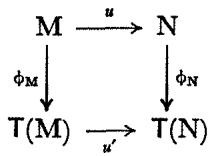
\includegraphics[keepaspectratio]{images/part003_fafbfb88.jpg}}

是可交换的。进一步地， \(u'\) 是分次代数同态。

存在性与唯一性 \(u'\) 由第 1 号命题 1 得出（把它应用于代数 \(T(N)\) 以及线性映射 \(\phi_N \circ u: M \to T(N)\) ）；由于

\[
u (\mathbf {M}) \subset \mathsf {T} ^ {1} (\mathbf {N}) = \mathbf {N},
\]

\(u'\) 是分次代数同态这一事实由第 1 号的注记得出。

命题 2 中的同态 \(u'\) 此后将记为 \(T(u)\) 。若 \(P\) 是一个 A-模，且 \(v: N \to P\) 是一个A-线性映射，则

\[
\mathsf {T} (v \circ u) = \mathsf {T} (v) \circ \mathsf {T} (u)\tag{4}
\]

因为 \(\mathsf{T}(v)\circ \mathsf{T}(u)\) 是使下图交换的代数同态

\pandocbounded{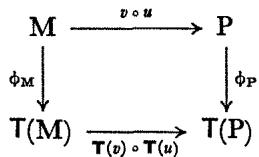
\includegraphics[keepaspectratio]{images/part003_f792dba1.jpg}}

\(\mathsf{T}(u)\) 有时称为 u 到 \(\mathsf{T}(\mathbf{M})\) （它包含 \(\mathbf{M} = \mathsf{T}^1(\mathbf{M})\) ）的典范扩张。注意，限制 \(\mathsf{T}^n(u): \mathsf{T}^n(\mathbf{M}) \to \mathsf{T}^n(\mathbf{N})\) 正是线性映射 \(u^{\otimes n} = u \otimes u \otimes \cdots \otimes u\) （n次），这由下式可知：

\[
\mathsf {T} ^ {n} (u) \left(x _ {1} \otimes \dots \otimes x _ {n}\right) = u \left(x _ {1}\right) \otimes \dots \otimes u \left(x _ {n}\right)
\]

因为 \(\mathsf{T}(u)\) 是一个代数同态且 \(\mathsf{T}^{1}(u)=u\) ；限制 \(\mathsf{T}^{0}(u)\) 在A上是恒等映射。 \(\mathsf{T}^{n}(u)\) 称为u的第n次张量幂。

命题3. 若 \(u: \mathbf{M} \to \mathbf{N}\) 是满射的A-线性映射，则同态 \(\mathsf{T}(u): \mathsf{T}(\mathbf{M}) \to \mathsf{T}(\mathbf{N})\) 是满射的，且其核是 \(\mathsf{T}(\mathbf{M})\) 的由核 \(\mathbf{P} \subset \mathbf{M} \subset \mathsf{T}(\mathbf{M})\) （即 \(u\) 的核）生成的双边理想。

\(T^{0}(u):T^{0}(M)\rightarrow T^{0}(N)\) 是双射的，且对每个整数 n\textgreater0,

\[
\mathbf {T} ^ {n} (u): \mathbf {T} ^ {n} (\mathbf {M}) \rightarrow \mathbf {T} ^ {n} (\mathbf {N})
\]

是满射的，这可通过对 \(n\) 作归纳并利用 II，§ 3，第 6 号，命题 6 看出；后一命题还表明（同样对 \(n\) 作归纳）， \(\mathfrak{S}_n\) （即 \(\mathsf{T}^n(u)\) 的核）是 \(\mathsf{T}^n(\mathbf{M})\) 中由乘积

\[
x _ {1} \otimes x _ {2} \otimes \dots \otimes x _ {n}
\]

生成，其中至少有一个 \(x_{i}\) 属于 \(\mathbf{P}\) 。这表明核 \(\mathfrak{S} = \bigoplus_{n\geqslant 1}\mathfrak{S}_n\) （即 \(\mathsf{T}(u)\) 的核）是由 \(\mathbf{P}\) 在 \(\mathsf{T}(\mathbf{M})\) 中生成的双边理想。

若 \(u: \mathbf{M} \to \mathbf{N}\) 是单射线性映射，则 \(\mathbf{T}(u)\) 并不总是单射映射（练习1）。然而，当 \(u\) 是使 \(u(\mathbf{M})\) 成为 \(\mathbf{N}\) 中直因子的单射时，结论成立，因为此时存在一个线性映射 \(v: \mathbf{N} \to \mathbf{M}\) ，使得 \(v \circ u\) 是 \(\mathbf{M}\) 上的恒等映射，从而

\[
\mathsf {T} (v \circ u) = \mathsf {T} (v) \circ \mathsf {T} (u)
\]

是 \(\mathsf{T}(\mathbf{M})\) 上的恒等映射，因此 \(\mathsf{T}(u)\) 是单射的，且其像（同构于 \(\mathsf{T}(\mathbf{M})\) ）是 \(\mathsf{T}(\mathbf{N})\) 的直因子（II，§1，第9号，命题15）。更精确地说：

命题4. 设N和P是A-模M的两个子模，使得它们的和 \(N + P\) 是M中的直因子，且它们的交 \(N \cap P\) 是N和P中的直因子。则同态 \(\mathsf{T}(\mathbf{N}) \to \mathsf{T}(\mathbf{M})\) , \(\mathsf{T}(\mathbf{P}) \to \mathsf{T}(\mathbf{M})\) 和

\[
\mathsf {T} (\mathbf {N} \cap \mathbf {P}) \rightarrow \mathsf {T} (\mathbf {M}),
\]

典范单射的典范扩张是单射；如果 \(\mathsf{T}(\mathbf{N})\) , \(\mathsf{T}(\mathbf{P})\) 和 \(\mathsf{T}(\mathbf{N} \cap \mathbf{P})\) 通过这些同态被等同于 \(\mathsf{T}(\mathbf{M})\) 的子代数，则

\[
\mathsf {T} (\mathbf {N} \cap \mathbf {P}) = \mathsf {T} (\mathbf {N}) \cap \mathsf {T} (\mathbf {P}).\tag{5}
\]

根据假设，存在子模 \(N' \subset N\) 和 \(P' \subset P\) ，使得 \(N = N' \oplus (N \cap P)\) , \(P = P' \oplus (N \cap P)\) ；于是

\[
\mathbf {N} + \mathbf {P} = \mathbf {N} ^ {\prime} \oplus \mathbf {P} ^ {\prime} \oplus (\mathbf {N} \cap \mathbf {P})
\]

并且根据假设存在子模 \(M'\) ⊂ M，使得

\[
\begin{array}{c} \mathbf {M} = \mathbf {M} ^ {\prime} \oplus (\mathbf {N} + \mathbf {P}) = \mathbf {M} ^ {\prime} \oplus \mathbf {N} ^ {\prime} \oplus \mathbf {P} ^ {\prime} \oplus (\mathbf {N} \cap \mathbf {P}) \\ = \mathbf {M} ^ {\prime} \oplus \mathbf {P} ^ {\prime} \oplus \mathbf {N} = \mathbf {M} ^ {\prime} \oplus \mathbf {N} ^ {\prime} \oplus \mathbf {P}. \end{array}
\]

特别地， \(N + P\) ，N，P以及 \(N \cap P\) 是M中的直因子，这（如前所述）意味着典范同态

\[
\begin{array}{l} \mathsf {T} (\mathbf {N} + \mathbf {P}) \to \mathsf {T} (\mathbf {M}), \qquad \mathsf {T} (\mathbf {N}) \to \mathsf {T} (\mathbf {M}), \\ \mathsf {T} (\mathbf {P}) \to \mathsf {T} (\mathbf {M}), \qquad \mathsf {T} (\mathbf {N} \cap \mathbf {P}) \to \mathsf {T} (\mathbf {M}) \end{array}
\]

是单射的。三个代数 \(\mathsf{T}(\mathbf{N})\) , \(\mathsf{T}(\mathbf{P})\) 和 \(\mathsf{T}(\mathbf{N} \cap \mathbf{P})\) 因此被等同于 \(\mathsf{T}(\mathbf{N} + \mathbf{P})\) 的子代数，而后者被等同于 \(\mathsf{T}(\mathbf{M})\) 的子代数；

记 \(\mathbf{Q} = \mathbf{N} \cap \mathbf{P}\) ，则只需证明：若 \(\mathsf{T}(\mathbf{Q})\) , \(\mathsf{T}(\mathbf{N}' \oplus \mathbf{Q})\) 和 \(\mathsf{T}(\mathbf{P}' \oplus \mathbf{Q})\) 通过这些同态被等同于 \(\mathsf{T}(\mathbf{N}' \oplus \mathbf{P}' \oplus \mathbf{Q})\) 的子代数，则

\[
\mathsf {T} (\mathbf {N} ^ {\prime} \oplus \mathbf {Q}) \cap \mathsf {T} (\mathbf {P} ^ {\prime} \oplus \mathbf {Q}) = \mathsf {T} (\mathbf {Q}).\tag{6}
\]

现在，考虑交换图

\pandocbounded{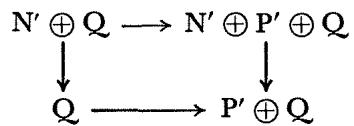
\includegraphics[keepaspectratio]{images/part003_8d12e188.jpg}}

其中水平箭头是典范单射，垂直箭头是典范投影。我们由此导出一个交换图

\begin{enumerate}
\def\labelenumi{(\arabic{enumi})}
\setcounter{enumi}{6}
\tightlist
\item
\end{enumerate}

\pandocbounded{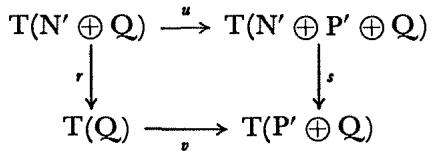
\includegraphics[keepaspectratio]{images/part003_389443db.jpg}}

其中 r 和 s 是满同态（命题 3），而 u 和 v 是单同态。因此，为证明 (6)，注意到右端显然包含于左端；于是只需验证：若

\[
x \in \mathsf {T} (\mathbf {N} ^ {\prime} \oplus \mathbf {Q}) \cap \mathsf {T} (\mathbf {P} ^ {\prime} \oplus \mathbf {Q}),
\]

那么 \(x \in \mathsf{T}(\mathsf{Q})\) 。现在，同态 s 的定义表明，它在 \(\mathsf{T}(\mathsf{P}' \oplus \mathsf{Q})\) （等同于 \(\mathsf{T}(\mathsf{N}' \oplus \mathsf{P}' \oplus \mathsf{Q})\) 的一个子代数）上的限制是恒等映射；因此关于 x 的假设蕴含 \(s(u(x)) = x\) 。但此时也有 \(v(r(x)) = x\) ，换言之，x 属于 \(\mathsf{T}(\mathsf{Q})\) 在 \(\mathsf{T}(\mathsf{P}' \oplus \mathsf{Q})\) 中的像，这就是要证明的。

注。特别地，当 A 是域时（II，§ 7，第 3 号，命题 4），命题 4 的假设对 M 的任意子模 N, P 总是成立。此外，若 N ⊂ P 且 N ≠ P，则对所有 n ≥ 1 有 T \(^{n}\) (N) ≠ T \(^{n}\) (P)，因为如果 R 是 P 在 N 中的补，则 T \(^{n}\) (P) ∩ T \(^{n}\) (R) = \{0\} 由(4)及T \(^{n}\) (R) ≠ \{0\}.

推论。设K是一个交换域，M是K上的一个向量空间。对于每一个元素 \(z \in \mathsf{T}(\mathbf{M})\) 存在一个M的最小子空间N，使得 \(z \in \mathsf{T}(\mathbf{N})\) 且N在K上具有有限秩。

在这个陈述中约定，对于 M 的每个向量子空间 P， \(T(P)\) 典范地等同于 \(T(M)\) 的一个子代数。设 \(z \in T(M)\) ；z 可以表示为一些元素的线性组合，其中每个元素都是 \(M = T^{1}(M)\) 中元素的有限乘积；出现在这些乘积中的 M 的所有元素生成一个有限秩的向量子空间 Q，且 \(z \in T(Q)\) .

设 \(\mathfrak{F}\) 为由有限秩向量子空间 \(\mathbf{P}\) （满足 \(z\in \mathsf{T}(\mathbf{P})\) ）组成的（非空）集合。 \(\mathfrak{F}\) 中元素的每个递减序列都是平稳的，因为它们是有限秩的向量空间。因此 \(\mathfrak{F}\) 有一个极小元素 \(\mathbf{N}\) （集合论，III，§6，第5号）。还需验证每个 \(\mathbf{P}\in \mathfrak{F}\) 包含 \(\mathbf{N}\) ；现在， \(z\in \mathsf{T}(\mathbf{P})\cap \mathsf{T}(\mathbf{N}) = \mathsf{T}(\mathbf{P}\cap \mathbf{N})\) （命题4）；根据 \(\mathbf{N}\) 的定义，这意味着 \(\mathbf{N}\cap \mathbf{P} = \mathbf{N}\) ，即 \(\mathbf{P}\supset \mathbf{N}\) .

M的子空间N称为与z相关联的。

\subsection{标量环的扩张}

设A，A'为两个交换环，且 \(\rho:A\to A'\) 为一个环同态。设M为一个A-模，M'为一个A'-模，且 \(u:M\to M'\) 为一个A-同态；由于典范单射 \(\phi_{M'}:M'\to T_{A'}(M')\) （通过标量限制）也是一个A-同态，所以复合映射 \(M\xrightarrow{u}M'\xrightarrow{\phi_{M'}}T_{A'}(M')\) 也是A-同态。由（第 2 号）导出一个 A-代数同态 \(T_{A}(M)\to\rho*(T_{A'}(M'))\) ，也记为 \(T(u):T_{A}(M)\to T_{A'}(M')\) ，它是使图表交换的唯一 A-同态。

\begin{enumerate}
\def\labelenumi{(\arabic{enumi})}
\setcounter{enumi}{7}
\tightlist
\item
\end{enumerate}

\pandocbounded{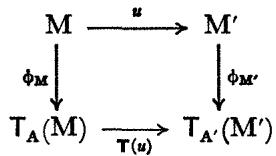
\includegraphics[keepaspectratio]{images/part003_9672ae23.jpg}}

若 \(\sigma: \mathbf{A}' \to \mathbf{A}''\) 是一个交换环同态， \(\mathbf{M}''\) 是一个 \(\mathbf{A}''\) -模，且 \(v: \mathbf{M}' \to \mathbf{M}''\) 是一个 \(\mathbf{A}'\) -同态，则上述唯一性性质表明

\[
\mathbf {T} (v \circ u) = \mathbf {T} (v) \circ \mathbf {T} (u).\tag{9}
\]

命题5. 设A，B为两个交换环， \(\rho: \mathbf{A} \to \mathbf{B}\) 一个环同态，且 M 是一个 A-模。典范扩张

\[
\psi : \mathsf {T} _ {\mathbf {B}} (\mathbf {B} \otimes_ {\mathbf {A}} \mathbf {M}) \rightarrow \mathbf {B} \otimes_ {\mathbf {A}} \mathsf {T} _ {\mathbf {A}} (\mathbf {M})
\]

（它是 B-线性映射 \(\mathbf{1}_{\mathbf{B}} \otimes \phi_{\mathbf{M}}: \mathbf{B} \otimes_{\mathbf{A}} \mathbf{M} \to \mathbf{B} \otimes_{\mathbf{A}} \mathsf{T}_{\mathbf{A}}(\mathbf{M})\) 的典范扩张）是分次 B-代数的同构。

考虑两个A-代数同态：典范单射 \(j: \mathbf{B} = \mathsf{T}^0(\mathbf{B} \otimes_{\mathbf{A}} \mathbf{M}) \to \mathsf{T}(\mathbf{B} \otimes_{\mathbf{A}} \mathbf{M})\) 及同态

\[
h = \mathsf {T} (i): \mathsf {T} (\mathbf {M}) \rightarrow \mathsf {T} (\mathbf {B} \otimes_ {\mathbf {A}} \mathbf {M})
\]

由典范 A-线性映射导出（参见公式 (8)），

\[
i: \mathbf {M} \rightarrow \mathbf {B} \otimes_ {\mathbf {A}} \mathbf {M}.
\]

由于 \(\mathsf{T}^0 (\mathbf{B}\otimes_{\mathbf{A}}\mathbf{M})\) 包含于 \(\mathsf{T}(\mathbf{B}\otimes_{\mathbf{A}}\mathbf{M})\) 的中心，可以应用 §4 第 2 号的命题 5，从而得到一个 A-代数同态

\[
\psi^ {\prime}: \mathbf {B} \otimes_ {\mathbf {A}} \mathsf {T} (\mathbf {M}) \rightarrow \mathsf {T} (\mathbf {B} \otimes_ {\mathbf {A}} \mathbf {M})
\]

，使得对于 \(\beta \in \mathbf{B}\) , \(x_{i} \in \mathbf{M}\) （ \(1 \leqslant i \leqslant n\) ），

\[
\psi^ {\prime} (\beta \otimes (x _ {1} \otimes x _ {2} \otimes \dots \otimes x _ {n})) = \beta ((1 \otimes x _ {1}) \otimes (1 \otimes x _ {2}) \otimes \dots \otimes (1 \otimes x _ {n})),
\]

这立即表明 \(\psi'\) 也是一个B-代数同态。只需证明 \(\psi \circ \psi'\) 和 \(\psi' \circ \psi\) 分别是 \(B \otimes_{A} T(M)\) 和 \(T(B \otimes_{A} M)\) 上的恒等映射。现在，这两个代数都由 \(B \otimes_{A} M\) 生成，并且显然 \(\psi \circ \psi'\) 和 \(\psi' \circ \psi\) 与 \(B \otimes_{A} M\) 上的恒等映射一致，由此得出结论。

\subsection{张量代数的正向极限}

设 \((\mathbf{A}_{\alpha},\phi_{\beta \alpha})\) 为一个交换环的有向正向系统，且 \((\mathbf{M}_{\alpha},f_{\beta \alpha})\) 为一个由 \(\mathbf{A}_{\alpha}\) -模构成的正向系统（II，§ 6，第 2 号）；设 \(\mathbf{A} = \varinjlim \mathbf{A}_{\alpha}\) 和 \(\mathbf{M} = \varinjlim \mathbf{M}_{\alpha}\) ，后者是一个 A-模。对于 \(\alpha \leqslant \beta\) ，一个 \(\mathbf{A}_{\alpha}\) -代数同态（第 3 号，公式 (8)） \(f_{\beta \alpha}' = \mathsf{T}(f_{\beta \alpha})\colon \mathsf{T}_{\mathbf{A}_{\alpha}}(\mathbf{M}_{\alpha})\to \mathsf{T}_{\mathbf{A}_{\beta}}(\mathbf{M}_{\beta})\) 由 \(\mathbf{A}_{\alpha}\) -同态 \(f_{\beta \alpha}\colon \mathbf{M}_{\alpha}\to \mathbf{M}_{\beta}\) 典范地导出，并且由（9）（第 3 号）可知 \((\mathsf{T}_{\mathbf{A}_{\alpha}}(\mathbf{M}_{\alpha}),f_{\beta \alpha}')\) 是一个由 \(\mathbf{A}_{\alpha}\) -代数构成的正向系统。另一方面，设 \(f_{\alpha}\colon \mathbf{M}_{\alpha}\to \mathbf{M}\) 为典范 \(\mathbf{A}_{\alpha}\) -同态；一个 \(\mathbf{A}_{\alpha}\) -代数同态 \(f_{\alpha}'\colon \mathsf{T}_{\mathbf{A}_{\alpha}}(\mathbf{M}_{\alpha})\to \mathsf{T}_{\mathbf{A}}(\mathbf{M})\) 由（第 3 号，公式 (8)）导出，并且由（9）（第 3 号）也可得出，诸 \(f_{\alpha}'\) 构成一个由 \(\mathbf{A}_{\alpha}\) -同态构成的正向系统。

命题6. A-同态 \(f' = \varinjlim f_{\alpha}' : \varinjlim T_{A_{\alpha}}(M_{\alpha}) \to T_{A}(M)\) 是一个分次代数同构。

为简化起见，我们记 \(\mathbf{E} = T_{\mathbf{A}}(\mathbf{M})\) 和 \(\mathbf{E}' = \varinjlim T_{\mathbf{A}_{\alpha}}(\mathbf{M}_{\alpha})\) ，并设

\[
g _ {\alpha}: \mathsf {T} _ {\mathrm{A} _ {\alpha}} (\mathbf {M} _ {\alpha}) \rightarrow \mathbf {E} ^ {\prime}
\]

为典范 \(\mathbf{A}_{\alpha}\) -同态。显然，复合 \(\mathbf{A}_{\alpha}\) -线性映射 \(\mathbf{M}_{\alpha} \xrightarrow{\phi_{\mathbf{M}_{\alpha}}} \mathsf{T}_{\mathbf{A}_{\alpha}}(\mathbf{M}_{\alpha}) \xrightarrow{g_{\alpha}} \mathbf{E}'\) 构成一个正向系统，因此存在唯一的 A-线性映射 \(u = \varinjlim (g_{\alpha} \circ \phi_{\mathbf{M}_{\alpha}}): \mathbf{M} \to \mathbf{E}'\) ，使得

\[
u \circ f _ {\alpha} = g _ {\alpha} \circ \phi_ {M _ {\alpha}}
\]

对所有 \(\alpha\) 成立。该映射本身唯一地分解（第 1 号，命题 1）为 \(\mathbf{M} \xrightarrow{\phi_{\mathbf{M}}} \mathrm{E} \to \mathrm{E}'\) ，其中 \(h\) 是一个 A-代数同态。只需证明 \(h \circ f' = 1_{\mathrm{E}'}\) 和 \(f' \circ h = 1_{\mathrm{E}}\) .

为此注意到，对于每个指标 \(\alpha\) （第3号，公式（8））

\[
h \circ f _ {\alpha} ^ {\prime} \circ \phi_ {M _ {\alpha}} = h \circ \phi_ {M} \circ f _ {\alpha} = u \circ f _ {\alpha} = g _ {\alpha} \circ \phi_ {M _ {\alpha}}
\]

由此，根据第1号命题1的唯一性断言，

\[
h \circ f _ {\alpha} ^ {\prime} = g _ {\alpha}
\]

对所有 \(\alpha\) 成立；由此可得 \((h \circ f') \circ g_{\alpha} = g_{\alpha}\) 对所有 \(\alpha\) 成立，因此由正向极限的定义得 \(h \circ f' = 1_{\mathbf{E}'}\) 。

另一方面，根据第3号公式（8），

\[
f ^ {\prime} \circ u \circ f _ {\alpha} = f ^ {\prime} \circ g _ {\alpha} \circ \phi_ {M _ {\alpha}} = f _ {\alpha} ^ {\prime} \circ \phi_ {M _ {\alpha}} = \phi_ {M} \circ f _ {\alpha},
\]

由此再次得到 \(f' \circ u = \phi_{\mathbb{M}}\) （由正向极限的定义）；我们得出 \(f' \circ h \circ \phi_{\mathbb{M}} = \phi_{\mathbb{M}}\) ，而第 1 号命题 1 的唯一性性质给出 \(f' \circ h = 1_{\mathbb{E}}\) .

命题6也可以通过观察以下事实来证明：对于每个整数 \(n \geqslant 1\) ，存在一个典范的 A-模同构 \(\lim_{\longrightarrow} \mathsf{T}_{\mathbf{A}_{\alpha}}^{n}(\mathbf{M}_{\alpha}) \to \mathsf{T}_{\mathbf{A}}^{n}(\mathbf{M})\) ，这由 II，§6，第3号，命题7通过对 \(n\) 作归纳得到。立即可验证，这些同构都是 \(f'\) 的限制。

\subsection{直和的张量代数。自由模的张量代数。分次模的张量代数。}

设 A 是一个交换环，且 \(M = \bigoplus_{\lambda \in L} M_{\lambda}\) 是一族A-模的直和。由II，§3，第7号，命题7，通过对n归纳可知， \(T^{n}(M)\) 是子模的直和，这些子模是典范单射的像

\[
\mathbf {M} _ {\lambda_ {1}} \otimes \mathbf {M} _ {\lambda_ {2}} \otimes \dots \otimes \mathbf {M} _ {\lambda_ {n}} \rightarrow \mathsf {T} ^ {n} (\mathbf {M}) = \mathbf {M} ^ {\otimes n}
\]

相对于所有序列 \((\lambda_{i})\in\mathbf{L}^{n}\) 。将 \(M_{\lambda_{1}}\otimes M_{\lambda_{2}}\otimes\cdots\otimes M_{\lambda_{n}}\) 与这个像等同，可以看出 \(T(\mathbf{M})\) 是下列模的直和

\[
\mathbf {M} _ {\lambda_ {1}} \otimes \mathbf {M} _ {\lambda_ {2}} \otimes \dots \otimes \mathbf {M} _ {\lambda_ {n}}
\]

（其中 \(n\) 遍历 \(\mathbf{N}\) ，且对每个 \(n\) ， \((\lambda_t)\) 遍历 \(\mathbf{L}^n\) .

我们首先推导出以下结论：

定理1. 设A为交换环，M为自由A-模，且 \((e_{\lambda})_{\lambda \in L}\) 为 M 的一组基。则诸元素 \(e_{s} = e_{\lambda_{1}} \otimes e_{\lambda_{2}} \otimes \cdots \otimes e_{\lambda_{n}}\) ——其中 \(s = (\lambda_{1}, \ldots, \lambda_{n})\) 遍历 L 中元素的所有有限序列的集合，而 \(e_{\varnothing}\) 用来表示 T(M) 的单位元——构成 A-模 T(M) 的一组基。

该基的元素显然是齐次的，且乘法表由下式给出

\[
e _ {s} e _ {t} = e _ {s t}\tag{10}
\]

（其中 \(st\) 表示由 \(\mathbf{L}\) 中元素组成的、通过并置序列 \(s\) 和 \(t\) 而得到的序列（I，§7，第2号）。

可以看出，T(M) 的基 \((e_{s})\) 连同乘法法则 (10) 典范同构于集合 L 上的自由幺半群（I，§7，第2号），该同构通过把这个幺半群的每个字 s 映到元素 \(e_{s}\) 而得到。由此（§2，第7号）可知，自由模 M（其基的指标集为 L）的张量代数 T(M) 典范同构于 L 在 A 上的自由结合代数。特别地（§2，第7号，命题7），对于每个从 L 到 A-代数 E 的映射 \(f: L \to E\) ，存在唯一的 A-代数同态 \(\bar{f}: T(M) \to E\) ，使得 \(\bar{f}(e_{\lambda}) = f(\lambda)\) 。

注。上述结果同样可以由自由结合代数和张量代数的泛性质推出，利用II，§3，第7号，命题7的推论2。

推论. 若 M 是投射 A-模，则 T(M) 是投射 A-模。

M 是自由 A-模 N 的一个直因子（II，§2，第 2 号，命题 4），因此 T(M) 是 T(N) 的一个直因子（第 2 号）；由于 T(N) 是自由的（定理 1），这表明 T(M) 是投射的（II，§2，第 2 号）。

命题7. 设 \(\Delta\) 是一个交换幺半群， \(\mathbf{M}\) 是一个 \(\Delta\) 型分次 A-模，而 \((\mathbf{M}_{\alpha})_{\alpha \in \Delta}\) 是其分次。对于每个有序对 \((\alpha, n) \in \Delta \times \mathbf{N}\) ，设 \(\mathsf{T}^{\alpha,n}(\mathbf{M})\) 为诸子模 \(\mathbf{M}_{\alpha_1} \otimes \mathbf{M}_{\alpha_2} \otimes \dots \otimes \mathbf{M}_{\alpha_n}\) （属于 \(\mathsf{T}^n(\mathbf{M})\) ，满足 \(\sum_{i=1}^{n} \alpha_i = \alpha\) ）的（直）和；于是 \((T^{\alpha, n}(M))_{(\alpha, n) \in \Delta \times N}\) 是唯一的 \(\Delta \times N\) 型分次，它与 \(T(M)\) 上的代数结构相容、并在 \(M = T^1(M)\) 上诱导出给定的分次。

在本号开头已经看到， \(\mathsf{T}(\mathbf{M})\) 是诸 \(\mathsf{T}^{\alpha,n}(\mathbf{M})\) 的直和，而这是一个与代数结构相容的分次这一事实直接由定义得出。若 \((\mathsf{T}'^{\alpha,n})\) 是另一个 \(\Delta \times \mathbf{N}\) 型分次，它在 \(\mathsf{T}(\mathbf{M})\) 上与代数结构相容且满足 \(\mathsf{T}^{\alpha,1}(\mathbf{M}) = \mathsf{T}'^{\alpha,1}\) （对 \(\alpha \in \Delta\) ），则直接由定义可知，对所有 \(n \geqslant 1\) 以及所有 \(\alpha \in \Delta\) ，有 \(\mathsf{T}^{\alpha,n}(\mathbf{M}) \subset \mathsf{T}'^{\alpha,n}\) ；但由于 \(\mathsf{T}(\mathbf{M})\) 也是诸 \(\mathsf{T}^{\alpha,n}(\mathbf{M})\) 的直和，这意味着 \(\mathsf{T}'^{\alpha,n} = \mathsf{T}^{\alpha,n}(\mathbf{M})\) (II，§1，第8号，注记)。

\subsection{张量与张量记号}

设 A 是一个交换环，M 是一个 A-模， \(\mathbf{M}^*\) 为 M 的对偶（II，§2，第3号），I 和 J 为两个不相交的有限集；A-模 \(\bigotimes_{i\in \mathrm{I}\cup \mathrm{J}}\mathbf{E}_i\) （其中 \(\mathbf{E}_i = \mathbf{M}\) （若 \(i\in \mathrm{I}\) ）， \(\mathbf{E}_i = \mathbf{M}^*\) （若 \(i\in \mathrm{J}\) ））记作 \(\mathsf{T}_{\mathsf{J}}^{\mathsf{I}}(\mathbf{M})\) ； \(\mathsf{T}_{\mathsf{J}}^{\mathsf{I}}(\mathbf{M})\) 的元素称为 M 上的 (I,J) 型张量。当 \(\mathbf{J} = \varnothing\) 时它们称为反变张量，当 \(\mathbf{I} = \varnothing\) 时称为协变张量，其余情形称为混合张量。

设 \(I'\) , \(I''\) 为 I 的两个子集，且 \(J'\) , \(J''\) 为 J 的两个子集，使得 \(I' \cup I'' = I\) , \(\mathbf{I}' \cap \mathbf{I}'' = \varnothing, \mathbf{J}' \cup \mathbf{J}'' = \mathbf{J}, \mathbf{J}' \cap \mathbf{J}'' = \varnothing\) ；则存在一个典范的结合同构（II，§3，第9号）

\[
\mathsf {T} _ {\mathbf {J}} ^ {\mathbf {I}} (\mathbf {M}) \rightarrow \mathsf {T} _ {\mathbf {J} ^ {\prime}} ^ {\mathbf {I} ^ {\prime}} (\mathbf {M}) \otimes_ {\mathbf {A}} \mathsf {T} _ {\mathbf {J} ^ {\prime \prime}} ^ {\mathbf {I} ^ {\prime \prime}} (\mathbf {M}).\tag{11}
\]

考虑张量代数 \(\mathsf{T}(\mathbf{M}\oplus \mathbf{M}^{*})\) ，由第 5 号可知 \(\mathsf{T}^n (\mathbf{M}\oplus \mathbf{M}^*)\) 典范地等同于诸 \(\mathsf{T}_{\mathbf{J}}^{\mathbf{I}}(\mathbf{M})\) 的直和，其中 I 遍历区间 \([1,n]\) （在 \(\mathbf{N}\) 中）的子集组成的集合，而 J 是 I 在 \([1,n]\) 中的补集。

当 \(I = [1, p]\) 且 \(J = [p + 1, p + q]\) ，其中整数 \(p \geqslant 0\) , \(q \geqslant 0\) （我们将 I（相应地 J）替换为 \(\varnothing\) ，如果 \(p = 0\) （相应地 \(q = 0\) ）），A-模 \(T_J^I(M)\) 也记作 \(T_q^p(M)\) ；A-模 \(T_0^n(M)\) 和 \(T_n^0(M)\) 根据定义分别是 A-模 \(T^n(M)\) 和 \(T^n(M^*)\) 。当 I 和 J 是基数为 \(p = \text{Card}(I)\) 和 \(q = \text{Card}(J)\) 的任意有限集合时，我们给它们每一个赋予一个全序；那么存在一个从 I（相应地 J）到 \([1, p]\) （相应地 \([p + 1, p + q]\) ）上的递增双射，因此这些双射定义了一个同构

\[
\mathbf {T} _ {\mathrm{J}} ^ {\mathrm{I}} (\mathbf {M}) \rightarrow \mathbf {T} _ {q} ^ {p} (\mathbf {M}).
\]

当 M 是有限生成的投射 A-模时，由 II，§ 2，第 7 号，命题 13 的推论 4 以及 II，§ 4，第 4 号，命题 4 的推论 1 可知，存在一个典范同构

\[
(\mathsf {T} _ {\mathbf {J}} ^ {\mathbf {I}} (\mathbf {M})) ^ {*} \to \mathsf {T} _ {\mathbf {I}} ^ {\mathbf {J}} (\mathbf {M}).
\]

现在假设 \(\mathbf{M}\) 是一个有限生成的自由 A-模，且设 \((e_{\lambda})_{\lambda \in L}\) 为 \(\mathbf{M}\) 的一组基（因此 L 是有限集）。 \(\mathbf{M}^*\) 的与 \((e_{\lambda})\) 对偶的基（II，§2，第 6 号）记为 \((e^{\lambda})_{\lambda \in L}\) 。基 \((e_{\lambda})\) 和 \((e^{\lambda})\) （分别属于 \(\mathbf{M}\) 和 \(\mathbf{M}^*\) ）定义了（第 5 号） \(\mathsf{T}_{\mathbf{J}}^{\mathbf{I}}(\mathbf{M})\) 的一个基，我们明确给出如下：给定两个映射 \(f\colon \mathbf{I} \to \mathbf{L}\) 和 \(g\colon \mathbf{J} \to \mathbf{L}\) ，设 \(e_f^g\) 为元素 \(\bigotimes_{i \in I \cup J} x_i\) （属于 \(\mathsf{T}_{\mathbf{J}}^{\mathbf{I}}(\mathbf{M})\) ），定义为

\[
x _ {i} = e _ {f (i)} \quad \text { if } i \in \mathbf {I}, \qquad x _ {i} = e ^ {g (i)} \quad \text { if } i \in \mathbf {J}.
\]

当 \((f, g)\) 遍历映射 \(f: \mathbf{I} \to \mathbf{L}\) 和 \(g: \mathbf{J} \to \mathbf{L}\) 的有序对组成的集合时，诸 \(e_f^g\) 构成 A-模 \(\mathsf{T}_{\mathbf{J}}^{\mathbf{I}}(\mathbf{M})\) 的一组基，称为与给定基 \((e_{\lambda})\) （ \(\mathbf{M}\) 的）相关联的基。对于 \(z \in \mathsf{T}_{\mathbf{J}}^{\mathbf{I}}(\mathbf{M})\) ，我们因此可以写出

\[
z = \sum_ {(f, g)} \alpha_ {g} ^ {f} (z). e _ {f} ^ {g}\tag{12}
\]

其中 \(\alpha_g^f\) 是关于基 \((e_f^g)\) 的坐标线性型；按照语言的约定俗成， \(\alpha_g^f(z)\) 称为张量 \(z\) 关于模 M 的基 \((e_\lambda)\) 的坐标。诸 \(\alpha_g^f\) 构成 \((e_g^f)\) 的对偶基，换言之，它们与 \(\mathsf{T}_{\mathbf{I}}^{\mathbf{j}}(\mathbf{M})\) 的基的元素等同，该基与 \((e_\lambda)\) 相关联。当 I 和 J 是 N 中区间 \([1,n]\) 的互补子集时， \(\alpha_g^f\) （或 \(\alpha_g^f(z)\) ）记法如下：每个元素 \(f(i)\) （对于 \(i\in I\) ）写作第 \(i\) 位上的上标，并在第 \(i\) 位处放一个点（对 \(i \in \mathbf{J}\) ）；类似地， \(g(i)\) （对于 \(i \in \mathbf{J}\) ）写作第 \(i\) 位上的下标，并在第 \(i\) 位处放一个点（对 \(i \in \mathbf{I}\) ）。例如，对于 \(\mathbf{I} = \{1, 4\}\) , \(\mathbf{J} = \{2, 3\}\) ，我们记 \(\alpha_{\cdot \nu \rho}^{\lambda \cdot \cdot \mu}\) ，如果 \(f(1) = \lambda, f(4) = \mu, g(2) = \nu, g(3) = \rho\) 。

设 \((\bar{e}_{\lambda})_{\lambda \in L}\) 为 M 的另一组基，且 \(P\) 为从 \((e_{\lambda})\) 到 \((\bar{e}_{\lambda})\) 的过渡矩阵（II，§ 10，第 8 号）。则从 \((e^{\lambda})\) 到 \((\bar{e}^{\lambda})\) （ \((\bar{e}_{\lambda}))\) 的对偶基）的过渡矩阵是 \(^{t}P^{-1}\) ，即 \(P\) 的逆步（II，§ 10，第 8 号，命题 5）。由此可得（II，§ 10，第 10 号），从基 \((e_{f}^{g})\) （属于 \(\mathrm{T}_{\mathrm{J}}^{\mathrm{I}}(\mathrm{M})\) ）到基 \((\bar{e}_{f}^{g})\) (其中 \(f\) （相应地 \(g\) ) 遍历从 I 到 L（相应地，从 J 到 L）的映射集合）的过渡矩阵是矩阵

\[
\bigotimes_ {i \in I \cup J} Q _ {i}, \quad \text { where } Q _ {i} = P \text { if } i \in I, Q _ {i} = ^ {t} P ^ {- 1} \text { if } i \in J.\tag{13}
\]

因此，该矩阵的转置被等同于

\[
\bigotimes_ {i \in \mathbf {I} \cup J} R _ {i}, \quad \text { where } R _ {i} = ^ {t} P ^ {- 1} \text { if } i \in \mathbf {I}, R _ {i} = P \text { if } i \in \mathbf {J}.\tag{14}
\]

现在假设 \(\mathbf{M}\) 是任意模。设 \(i\in \mathbf{I}, j\in \mathbf{J}\) 并记 \(\mathbf{I}' = \mathbf{I} - \{i\}, J' = J - \{j\}\) ；我们将定义一个典范的 A-线性映射

\[
c _ {j} ^ {i} \colon \mathsf {T} _ {\mathbf {J}} ^ {\mathbf {I}} (\mathbf {M}) \to \mathsf {T} _ {\mathbf {J} ^ {\prime}} ^ {\mathbf {I} ^ {\prime}} (\mathbf {M}),
\]

称为指标 \(i\) 与指标 \(j\) 的缩并。为此，注意到 \(\mathbf{M}^{\mathrm{I}} \times (\mathbf{M}^{*})^{\mathrm{J}}\) 上的映射，它将每个族 \((x_{i})_{i \in \mathbf{I} \cup \mathbf{J}}\) （其中 \(x_{i} \in \mathbf{M}\) （若 \(i \in \mathbf{I}\) ）， \(x_{i} \in \mathbf{M}^{*}\) （若 \(i \in \mathbf{J}\) ））对应到元素

\[
\left\langle x _ {i}, x _ {j} \right\rangle \otimes_ {k \in (\mathbb {I} \cup \mathbb {J}) - \{i, j \}} x _ {k}\tag{15}
\]

（属于 \(T_{J'}^{I'}(M)\) ）是 A-多重线性的； \(c_{j}^{i}\) 是对应的 A-线性映射。

现在假设 M 是自由且有限生成的，并令 \((e_{\lambda})_{\lambda \in L}\) 为 M 的一组基。给定两个映射 \(f: I \to L\) , \(g: J \to L\) ，设 \(f_i\) 表示 f 在 \(I' = I - \{i\}\) 上的限制， \(g_j\) 表示 g 在 \(J' = J - \{j\}\) 上的限制；于是根据 (12)

\[
c _ {j} ^ {i} (e _ {f} ^ {g}) = \left\{ \begin{array}{l l} 0 & \text { if } f (i) \neq g (j) \\ e _ {f _ {i}} ^ {g _ {j}} & \text { if } f (i) = g (j) \end{array} \right.\tag{16}
\]

\(c_j^i(z)\) 的坐标作为 \(z\) 的坐标的函数的表达式由此得出；对于每个映射 \(f'\) （相应地 \(g'\) ）——从 \(I'\) 到 \(L\) （相应地，从 \(J'\) 到 \(L\) ）——以及每个 \(\lambda \in L\) ，设 \((f', \lambda)\) （相应地 \((g', \lambda)\) ）表示从 \(I\) 到 \(L\) （相应地，从 \(J\) 到 \(L\) ）的、在 \(I'\) （相应地 \(J'\) ）上的限制为 \(f'\) （相应地 \(g'\) ）、并且以 \(\lambda\) 为其在元素 \(i\) （相应地 \(j\) ）处的值的映射。那么，若关于基 \((e_{f'}^{g'})\) （ \(T_{J'}^{I'}(M)\) 的基）的坐标线性型记为 \(\beta_{g'}^{f'}\) ,

\[
\beta_ {g ^ {\prime}} ^ {f ^ {\prime}} (c _ {j} ^ {i} (z)) = \sum_ {\lambda \in L} \alpha_ {(g ^ {\prime}, \lambda)} ^ {(f ^ {\prime}, \lambda)} (z).\tag{17}
\]

张量的例子。(1) 设 M 是有限生成的投射 A-模。我们知道（II，§ 4，第 2 号，命题 2 的推论），存在一个典范的 A-模同构

\[
\theta_ {\mathbf {M}} \colon \mathbf {M} ^ {*} \otimes_ {\mathbf {A}} \mathbf {M} \rightarrow \operatorname{End} _ {\mathbf {A}} (\mathbf {M})
\]

，使得 \(\theta_{\mathbf{M}}(x^{*}\otimes x)\) （对于 \(x\in \mathbf{M},x^{*}\in \mathbf{M}^{*}\) ）是自同态

\[
y \mapsto \langle y, x ^ {*} \rangle x.
\]

因此，借助 \(\theta_{\mathbf{M}}\) , \(\mathsf{T}_{(1)}^{(2)}(\mathbf{M})\) （同构于 \(\mathsf{T}_1^1 (\mathbf{M}))\) 可与 A-模 \(\operatorname{End}_{\mathbf{A}}(\mathbf{M})\) 等同。假设 \(\mathbf{M}\) 是自由模，且设 \((e_{\lambda})_{\lambda \in \mathbf{L}}\) 为 \(\mathbf{M}\) 的一组基；那么张量 \(z\in \mathbf{M}^*\otimes \mathbf{M}\) 关于该模的基 \((e^{\mu}\otimes e_{\lambda})\) 的坐标记为 \(\zeta_{\mu}^{\cdot \lambda}\) 。由于 \(\theta_{\mathrm{M}}(e^{\mu}\otimes e_{\lambda})\) 是自同态 \(y\mapsto \langle y,e^{\mu}\rangle e_{\lambda}\) ，自同态 \(u = \theta_{\mathrm{M}}(z) = \theta_{\mathrm{M}}\left(\sum_{\lambda ,\mu}\zeta_{\mu}^{\cdot \lambda}e^{\mu}\otimes e_{\lambda}\right)\) 把 \(y\) 映到 \(\sum_{\lambda ,\mu}\zeta_{\mu}^{\cdot \lambda}\langle y,e^{\mu}\rangle e_{\lambda}\) ；取 \(y = e_{\lambda}\) ，我们得到关系式

\[
u (e _ {\lambda}) = \sum_ {\mu \in L} \zeta_ {\lambda} ^ {\cdot \mu} e _ {\mu}\tag{18}
\]

换言之，线性映射 \(u = \theta_{\mathrm{M}}(z)\) 的矩阵是这样的矩阵：其位于指标 \(\mu\) 的行与指标 \(\lambda\) 的列交叉处的元素为 \(\zeta_{\lambda}^{\mu}\) 。

\(u\) 的迹的定义（II，§4，第3号）立即表明

\[
\operatorname{Tr} (\theta_ {\mathbb {M}} (z)) = c _ {1} ^ {2} (z).
\]

因此，元素 \(z_0 = \sum_{\lambda \in L} e^\lambda \otimes e_\lambda\) （其坐标 \(\zeta_\mu^{\cdot \lambda}\) 对于 \(\lambda \neq \mu\) 为零，对于 \(\lambda = \mu\) 等于1），它满足 \(\theta_M(z_0) = 1_M\) ，是元素 \(1 \in A = T_0^0(M)\) 在映射（缩并的转置）下的像。

\[
c _ {1} ^ {2}: \mathbf {T} _ {\{1 \}} ^ {\{2 \}} (\mathbf {M}) \rightarrow \mathbf {A}.
\]

\begin{enumerate}
\def\labelenumi{(\arabic{enumi})}
\setcounter{enumi}{1}
\tightlist
\item
  始终假设 M 是有限生成的投射 A-模；存在一个典范的 A-模同构
\end{enumerate}

\[
\mu : \mathbf {M} ^ {*} \otimes_ {\mathbf {A}} \mathbf {M} ^ {*} \rightarrow (\mathbf {M} \otimes_ {\mathbf {A}} \mathbf {M}) ^ {*}
\]

（II，§4，第 4 号，命题 2 的推论 1）以及一个典范同构

\[
\theta : (\mathbf {M} \otimes_ {\mathbf {A}} \mathbf {M}) ^ {*} \otimes_ {\mathbf {A}} \mathbf {M} \rightarrow \operatorname{Hom} _ {\mathbf {A}} (\mathbf {M} \otimes_ {\mathbf {A}} \mathbf {M}, \mathbf {M})
\]

（II，§4，第 2 号，命题 2 的推论）；此外 \(\operatorname{Hom}_{\mathbf{A}}(\mathbf{M} \otimes_{\mathbf{A}} \mathbf{M}, \mathbf{M})\) 典范同构于 A-模 \(\mathcal{L}_2(\mathbf{M}, \mathbf{M}; \mathbf{M})\) ，即由从 \(\mathbf{M} \times \mathbf{M}\) 到 \(\mathbf{M}\) 的 A-双线性映射组成的模（II，§3，第 9 号）。复合这些同构，得到典范同构

\[
\chi_ {\mathbf {M}} \colon T _ {\{1, 2 \}} ^ {(3)} (\mathbf {M}) = \mathbf {M} ^ {*} \otimes \mathbf {M} ^ {*} \otimes \mathbf {M} \rightarrow \mathcal {L} _ {2} (\mathbf {M}, \mathbf {M}; \mathbf {M})
\]

使得，对于 \(x^{*}, y^{*}\) （属于 \(\mathbf{M}^{*}\) ）， \(z \in \mathbf{M}\) ， \(\chi_{\mathbf{M}}(x^{*} \otimes y^{*} \otimes z)\) 是双线性映射

\[
(u, v) \mapsto \langle u, x ^ {*} \rangle \langle v, y ^ {*} \rangle z.
\]

因此，借助 \(\chi_{\mathbf{M}}\) , \(\mathsf{T}_{\{1,2\}}^{(3)}(\mathbf{M})\) （同构于 \(\mathsf{T}_{2}^{1}(\mathbf{M})\) ）可与 A-模 \(\mathcal{L}_2(\mathbf{M},\mathbf{M};\mathbf{M})\) 等同。假设 \(\mathbf{M}\) 是一个自由 A-模，且设 \((e_{\lambda})_{\lambda \in L}\) 为 \(\mathbf{M}\) 的一组基；那么张量 \(z\in \mathbf{M}^*\otimes \mathbf{M}^*\otimes \mathbf{M}\) 关于该模的基 \((e^{\lambda}\otimes e^{\mu}\otimes e_{\nu})\) 的坐标记为 \(\zeta_{\lambda \mu}^{\cdot \cdot \nu}\) 。双线性映射 \(\chi_{\mathbf{M}}(z)\) 把有序对 \((e_{\lambda},e_{\mu})\) 映到

\[
\sum_ {\nu \in L} \zeta_ {\lambda \mu}^{\cdot \cdot \nu} e _ {\nu}
\]

因此诸 \(\zeta_{\lambda \mu}^{\cdots \nu}\) 正是定义在 \(\mathbf{M}\) 上、由双线性映射 \(\chi_{\mathbf{M}}(z)\) 给出的（一般非结合的）代数关于基 \((e_{\lambda})\) 的结构常数（ \(\S 1\) ，第 7 号）。

注记2. 设 \((e_{\lambda})_{\lambda \in L}, (\tilde{e}_{\lambda})_{\lambda \in L}\) 为 M 的两个基，且 \(P\) 为从 \((e_{\lambda})\) 到 \((\tilde{e}_{\lambda})\) 的过渡矩阵。根据例1中所见， \(P\) 中位于指标 \(\lambda\) 的行与指标 \(\mu\) 的列交叉处的元素记为 \(\alpha_{\mu}^{\lambda}\) ，逆步 \(^{t}P^{-1}\) 中位于指标 \(\lambda\) 的行与指标 \(\mu\) 的列交叉处的元素记为 \(\beta_{\lambda}^{\mu}\) 。于是（采用上面引入的记号）

\begin{enumerate}
\def\labelenumi{(\arabic{enumi})}
\setcounter{enumi}{18}
\tightlist
\item
\end{enumerate}

\[
\left\{ \begin{array}{l} \tilde {e} _ {\mu} = \sum_ {\lambda} \alpha_ {\mu} ^ {\lambda} e _ {\lambda} \\ \tilde {e} ^ {\mu} = \sum_ {\lambda} \beta_ {\lambda} ^ {\mu} e ^ {\lambda} \end{array} \right.\tag{20}
\]

\[
\bar {e} _ {f ^ {\prime}} ^ {g ^ {\prime}} = \sum_ {(f, g)} \left(\prod_ {i \in I} \alpha_ {f ^ {\prime} (i)} ^ {f (i)}\right) \left(\prod_ {j \in J} \beta_ {g (j)} ^ {g ^ {\prime} (j)}\right) e _ {f} ^ {g}
\]

对于所有映射 \(f': \mathbf{I} \to \mathbf{L}\) 和 \(g': \mathbf{J} \to \mathbf{L}\) 成立。于是，坐标 \(\zeta_g^f\) ——张量 \(z \in \mathbb{T}_J^{\mathbf{I}}(\mathbf{M})\) 关于基 \((e_{\lambda})\) 的坐标——可以利用公式由坐标 \(\bar{\zeta}_{g'}^{f'}\) —— \(z\) 关于基 \((\bar{e}_{\lambda})\) 的坐标——表示出来

\[
\zeta_ {g} ^ {f} = \sum_ {(f ^ {\prime}, g ^ {\prime})} \left(\prod_ {i \in I} \alpha_ {f ^ {\prime} (i)} ^ {f (i)}\right) \left(\prod_ {j \in J} \beta_ {g (j)} ^ {g ^ {\prime} (j)}\right) \bar {\zeta} _ {g ^ {\prime}} ^ {f ^ {\prime}}.\tag{21}
\]

矩阵 \(P^{-1}\) （从基 \((\tilde{e}_{\lambda})\) 到基 \((e_{\lambda})\) 的过渡矩阵）是 \(^{t}P^{-1}\) 的转置，使得 \(\beta_{\lambda}^{\mu}\) 是位于指标 \(\lambda\) 的列与指标 \(\mu\) 的行交叉处、出现在 \(P^{-1}\) 中的元素。对 \(e_{f}^{g}\) （用 \(\tilde{e}_{f'}^{g'}\) 表示）以及对 \(\overline{\zeta}_{g'}^{f'}\) （用 \(\zeta_{g}^{f}\) 表示）的计算，因此是通过在上述计算中把 \(\alpha_{\mu}^{\lambda}\) 换为 \(\beta_{\lambda}^{\mu}\) 、把 \(\beta_{\lambda}^{\mu}\) 换为 \(\alpha_{\mu}^{\lambda}\) ，并交换 \(f\) 与 \(f'\) 以及 \(g\) 与 \(g'\) 的角色而得到的。则

\[
e _ {f} ^ {g} = \sum_ {(f ^ {\prime}, g ^ {\prime})} \left(\prod_ {j \in J} \alpha_ {g ^ {\prime} (j)} ^ {g (j)}\right) \left(\prod_ {i \in I} \beta_ {f (i)} ^ {f ^ {\prime} (i)}\right) \bar {e} _ {f ^ {\prime}} ^ {g ^ {\prime}}\tag{22}
\]

\[
\bar {\zeta} _ {g ^ {\prime}} ^ {f ^ {\prime}} = \sum_ {(f, g)} \left(\prod_ {j \in J} \alpha_ {g ^ {\prime} (j)} ^ {g (j)}\right) \left(\prod_ {i \in I} \beta_ {f (i)} ^ {f ^ {\prime} (i)}\right) \zeta_ {g} ^ {f}.\tag{23}
\]

上述公式的特点是求和针对那些分别作为下指标和上指标各出现一次的指标进行。某些作者鉴于这一情况，允许自己省略求和符号。

\section{对称代数}

\subsection{模的对称代数的定义}

定义 1. 设 A 为交换环，M 为 A-模。M 的对称代数，记为 S(M) 或 Sym(M)，或 \(S_{A}(M)\)，是张量代数 T(M) 关于双边理想 \(\mathfrak{J}'\) （也记作 \(\mathfrak{J}_{\mathbf{M}}'\) ）的商代数，该理想由 T(M) 的元素 \(xy - yx = x \otimes y - y \otimes x\) 生成，其中 \(x\) 和 \(y\) 遍历 M。

由于理想 \(\mathfrak{J}'\) 由次数为 2 的齐次元素生成，它是一个分次理想（II，§11，第3号，命题2）；我们记 \(\mathfrak{J}_n' = \mathfrak{J}' \cap T^n(M)\) ；代数 \(S(M)\) 于是由诸 \(S^n(M) = T^n(M)/\mathfrak{J}_n'\) 组成的分次（称为典范分次）进行分次。现在 \(\mathfrak{J}_0' = \mathfrak{J}_1' = \{0\}\) ，因此 \(S^0(M)\) 与 A 典范等同，而 \(S^1(M)\) 与 \(T^1(M) = M\) 等同；在后续内容中我们始终进行这些等同，并用 \(\phi'\) 或 \(\phi_M'\) 表示典范单射 \(M \to S(M)\) 。

命题1. 代数 \(\mathbf{S}(\mathbf{M})\) 是交换的。

根据定义 \(\phi'(x)\phi'(y) = \phi'(y)\phi'(x)\) （对 \(x, y\) 属于 \(\mathbf{M}\) ）；并且由于元素 \(\phi'(x)\) （其中 \(x\) 遍历 \(\mathbf{M}\) ）生成 \(\mathbf{S}(\mathbf{M})\) ，结论由 §1 第 7 号得出。

命题2. 设E是一个A-代数，且f: M → E是一个A-线性映射，使得

\[
f (x) f (y) = f (y) f (x) \text {   for   all   } x, y \text {   in   } \mathbf {M}.\tag{1}
\]

存在唯一的 A-代数同态 \(g \colon \mathbb{S}(\mathbf{M}) \to \mathbf{E}\) ，使得 \(f = g \circ \phi'\) 。

换言之， \((\mathbb{S}(\mathbf{M}), \phi')\) 是泛映射问题（集合论，IV，§3，第1号）的一个解，其中 \(\Sigma\) 是A-代数结构的类， \(\alpha\) -映射是满足(1)的从A-模M到A-代数的线性映射。

\(g\) 的唯一性由 \(\phi'(\mathbf{M}) = \mathbf{M}\) 生成 \(\mathbf{S}(\mathbf{M})\) 这一事实推出。为证明 \(g\) 的存在性，注意根据 §5 第 1 号命题 1，存在一个 A-代数同态 \(g_1: \mathbf{T}(\mathbf{M}) \to \mathbf{E}\) ，使得 \(f = g_1 \circ \phi\) ；

只需证明 \(g_1\) 在理想 \(\mathfrak{J}'\) 上为零即可，因为此时，若 \(p: \mathsf{T}(\mathbf{M}) \to \mathsf{S}(\mathbf{M}) = \mathsf{T}(\mathbf{M}) / \mathfrak{J}'\) 是典范同态，则可写 \(g_1 = g \circ p\) ，其中 \(g: \mathsf{S}(\mathbf{M}) \to \mathbf{E}\) 是一个代数同态，而结论将由 \(p \circ \phi = \phi'\) 这一事实得出。现在，\(g_1\) 的核是一个双边理想，由（1）及关系 \(g_1 \circ \phi = f\) ，它包含元素 \(x \otimes y - y \otimes x\) （对 \(x, y\) 属于 \(\mathbf{M}\) ）。这就完成了证明。

注：(1) 设 E 是一个 Z 型分次 A-代数，其分次为 \((\mathrm{E}_{n})\) ，并设线性映射 f （假定满足 (1)）满足

\[
f (\mathbf {M}) \subset \mathrm{E} _ {1}.\tag{2}
\]

则关系式 \(g(x_1x_2 \ldots x_p) = f(x_1)f(x_2) \ldots f(x_p)\) （其中 \(x_i \in \mathbf{M}\) ）表明 \(g(\mathbf{S}^p(\mathbf{M})) \subset \mathrm{E}_p\) 对所有 \(p \geqslant 0\) 成立，因此 \(g\) 是分次代数同态。

\begin{enumerate}
\def\labelenumi{(\arabic{enumi})}
\setcounter{enumi}{1}
\item
  \(\mathsf{S}(\mathbf{M})\) 的每一个元素都是形如 \(x_{1}x_{2}\ldots x_{n}\) （其中 \(x_{i}\) 属于 \(\mathbf{M}\) ）的乘积之和；应注意不要把 \(\mathsf{S}(\mathbf{M})\) 中所取的此类乘积与 \(\mathsf{T}(\mathbf{M})\) 中所取的类似乘积相混淆。
\item
  若 \(n!\) .1 在 A 中可逆，A-模 \(S^n(M)\) 由形如 \(x^n\) （其中 \(x \in M\) ）的元素生成；这由上述注记及 I，§8，第 2 号，命题 2 得出。
\end{enumerate}

\subsection{对称代数的函子性质}

命题 3. 设 A 为交换环，M 和 N 为两个 A-模，u: M → N 为 A-线性映射。则存在唯一的 A-代数同态 \(u'\) ：S(M) → S(N)，使得该图表

\pandocbounded{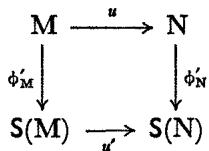
\includegraphics[keepaspectratio]{images/part003_0f38c769.jpg}}

是交换的。此外， \(u'\) 是分次代数同态。

\(u'\) 的存在性与唯一性由第 1 号命题 2 应用于交换代数 \(\mathbf{S}(\mathbf{N})\) 和 \(f = \phi_{\mathbf{N}}' \circ u: \mathbf{M} \to \mathbf{S}(\mathbf{N})\) 得出；由于

\[
f (\mathbf {M}) \subset \mathbf {S} ^ {1} (\mathbf {N}) = \mathbf {N},
\]

\(u'\) 是分次代数同态这一事实由第 1 号注记 1 得出。

命题 3 中的同态 \(u'\) 此后将记为 \(S(u)\) 。若 \(P\) 是一个 A-模，且 \(v: N \to P\) 是一个 A-线性映射，则

\[
\mathbf {S} (v \circ u) = \mathbf {S} (v) \circ \mathbf {S} (u)\tag{3}
\]

因为 \(\mathbf{S}(v) \circ \mathbf{S}(u)\) 是使下图交换的代数同态

\pandocbounded{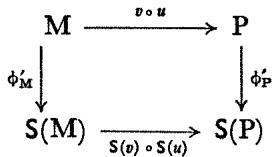
\includegraphics[keepaspectratio]{images/part003_67e6d402.jpg}}

由于 \(\mathbf{S}(\mathbf{M})\) 包含 \(\mathbf{M} = \mathbf{S}^1 (\mathbf{M})\) , \(\mathbf{S}(u)\) 有时称为 \(u\) 到 \(\mathbf{S}(\mathbf{M})\) 的典范扩张。限制 \(\mathbf{S}^n (u): \mathbf{S}^n (\mathbf{M}) \to \mathbf{S}^n (\mathbf{N})\) 满足

\[
\mathsf {S} ^ {n} (u) \left(x _ {1} x _ {2} \dots x _ {n}\right) = u \left(x _ {1}\right) u \left(x _ {2}\right) \dots u \left(x _ {n}\right)
\]

其中 \(x_{i} \in M\) ，因为 \(\mathbf{S}(u)\) 是一个代数同态且 \(\mathbf{S}^{1}(u) = u\) ；\(\mathbf{S}^{0}(u)\) 在 A 上的限制是恒等映射。注意， \(\mathbf{S}^{n}(u)\) 可以由 \(\mathbf{T}^{n}(u): \mathbf{T}^{n}(\mathbf{M}) \to \mathbf{T}^{n}(\mathbf{N})\) 通过过渡到商得到。

命题4. 若 \(u: \mathbf{M} \to \mathbf{N}\) 是满射 A-线性映射，则同态 \(\mathbf{S}(u): \mathbf{S}(\mathbf{M}) \to \mathbf{S}(\mathbf{N})\) 是满射的，且其核是 \(\mathbf{S}(\mathbf{M})\) 的由核 \(\mathbf{P} \subset \mathbf{M} \subset \mathbf{S}(\mathbf{M})\) （即 \(u\) 的核）生成的理想。

我们记 \(v = \mathsf{T}(u) \colon \mathsf{T}(\mathbf{M}) \to \mathsf{T}(\mathbf{N})\) ；我们知道（§5，第 2 号，命题 3） \(v\) 是满射的，因此由定义可知 \(v(\mathfrak{J}_{\mathbf{M}}') = \mathfrak{J}_{\mathbf{N}}'\) ；若 \(\Re\) 是 \(v\) 的核，则 \(v^{-1}(\mathfrak{J}_{\mathbf{N}}') = \Re + \mathfrak{J}_{\mathbf{M}}'\) 。由于 \(\mathsf{S}(u) \colon \mathsf{T}(\mathbf{M}) / \mathfrak{J}_{\mathbf{M}}' \to \mathsf{T}(\mathbf{N}) / \mathfrak{J}_{\mathbf{N}}'\) 是由 \(v\) 过渡到商而得到的，它是一个满射同态，其核为 \(\Re' = (\Re + \mathfrak{J}_{\mathbf{M}}') / \mathfrak{J}_{\mathbf{M}}'\) 。由于 \(\Re\) 由核 \(\mathbf{P}\) （即 \(u\) 的核）生成（§5，第 2 号），\(\Re'\) 亦然。

若 \(u: \mathbf{M} \to \mathbf{N}\) 是单射线性映射，\(\mathbf{S}(\mathbf{u})\) 并不总是单射映射（练习1）。然而，当 \(u\) 是使 \(u(\mathbf{M})\) 为 \(\mathbf{N}\) 中直因子的单射时，它是单射的，且此时 \(\mathbf{S}(u)\) 的像（同构于 \(\mathbf{S}(\mathbf{M})\) ）是 \(\mathbf{S}(\mathbf{N})\) 的一个直因子；其证明与关于 \(\mathbf{T}(u)\) 的类似断言（ \(\S 5\) ，第 2 号）的证明相同，只需把 \(\mathbf{T}\) 换为 \(\mathbf{S}\) 。

命题5. 设N和P是A-模M的两个子模，使得它们的和 \(N + P\) 是M中的直因子，且它们的交集 \(N \cap P\) 是N和P中的直因子。则同态 \(\mathsf{S}(\mathsf{N}) \to \mathsf{S}(\mathsf{M}), \mathsf{S}(\mathsf{P}) \to \mathsf{S}(\mathsf{M})\) 和

\[
\mathbf {S} (\mathbf {N} \cap \mathbf {P}) \rightarrow \mathbf {S} (\mathbf {M}),
\]

（即典范单射的典范扩张）都是单射的；如果 \(\mathbf{S}(\mathbf{N})\) , \(\mathbf{S}(\mathbf{P})\) 和 \(\mathbf{S}(\mathbf{N} \cap \mathbf{P})\) 通过这些同态被等同于 \(\mathbf{S}(\mathbf{M})\) 的子代数，则

\[
\mathbf {S} (\mathbf {N} \cap \mathbf {P}) = \mathbf {S} (\mathbf {N}) \cap \mathbf {S} (\mathbf {P}).\tag{4}
\]

证明归结为 §5，第 2 号，命题 4 的证明，只需通篇把 T 换为 S。当A是域时，命题5的假设对M的任意子模N、P总是成立。

推论。设K是一个交换域，M是K上的一个向量空间。对于每一个元素 \(z \in \mathbb{S}(\mathbf{M})\) 存在 M 的一个最小向量子空间 N，使得 \(z \in \mathbb{S}(\mathbf{N})\) 且N是有限维的。

证明的推导源自 §5，第 2 号，命题 4 的推论，只需通篇把 T 换为 S。

N 称为 M 的与 z 相关联的向量子空间。

\subsection{模的 n 次对称幂与对称多重线性映射}

设 X, Y 为两个集合，n 为整数 \(\geqslant1\) 。从 \(X^{n}\) 到 Y 的对称映射是指任意满足以下条件的映射 \(f: X^{n} \to Y\) ：对于每个置换 \(\sigma \in S_{n}\) 以及每个元素 \((x_{i}) \in X^{n}\) ，

\[
f (x _ {\sigma (1)}, x _ {\sigma (2)}, \dots , x _ {\sigma (n)}) = f (x _ {1}, x _ {2}, \dots , x _ {n}).\tag{5}
\]

由于交换两个相邻整数的对换生成群 \(\mathfrak{S}_n\) （I，§ 5，第 7 号），只需条件（5）对 \(\sigma\) 为这样一个对换的情形成立即可。

当 Y 是交换环 A 上的模时，显然从 \(X^{n}\) 到 Y 的对称映射的集合是 A-模 \(Y^{X^{n}}\) （由所有从 \(X^{n}\) 到 Y 的映射组成）的一个子模。

命题6. 设 A 是一个交换环，M 和 N 是两个 A-模。如果对每个 A-线性映射 \(g: \mathbf{S}^n(\mathbf{M}) \to \mathbf{N} (n \geqslant 1)\) 令其对应 n-线性映射

\[
\left(x _ {1}, x _ {2}, \dots , x _ {n}\right) \mapsto g \left(x _ {1} x _ {2} \dots x _ {n}\right)\tag{6}
\]

（其中右端的乘积取在代数 \(\mathbf{S}(\mathbf{M})\) 中），则得到 A-模 \(\operatorname{Hom}_{\mathbf{A}}(\mathbf{S}^{n}(\mathbf{M}), \mathbf{N})\) 到由对称 \(n\) -线性映射（从 \(\mathbf{M}^{n}\) 到 \(\mathbf{N}\) ）组成的 A-模上的一个双射 A-线性映射。

回忆（II，§3，第9号），存在从 A-模 \(\operatorname{Hom}_{\mathbf{A}}(\mathbb{T}^{n}(\mathbf{M}), \mathbf{N})\) 到 A-模 \(\mathcal{L}_{n}(\mathbf{M}, \ldots, \mathbf{M}; \mathbf{N})\) （由所有 \(n\) -线性映射（从 \(\mathbf{M}^{n}\) 到 \(\mathbf{N}\) ）组成）上的典范双射，它是通过把每个 A-线性映射 \(f: \mathbb{T}^{n}(\mathbf{M}) \to \mathbf{N}\) 对应到 \(n\) -线性映射而得到的

\[
\bar {f} \colon (x _ {1}, x _ {2}, \dots , x _ {n}) \mapsto f (x _ {1} \otimes x _ {2} \otimes \dots \otimes x _ {n}).\tag{7}
\]

另一方面，A-线性映射 \(g \colon \mathbb{S}^n(\mathbf{M}) \to \mathbf{N}\) 一一对应于满足以下条件的 A-线性映射 \(f \colon \mathbb{T}^n(\mathbf{M}) \to \mathbf{N}\) ：\(f\) 在 \(\mathfrak{J}_n'\) 上为零；对应方式是把 \(g\) 对应到映射 \(f = g \circ p_n\) ，其中

\[
p _ {n} \colon \mathbf {T} ^ {n} (\mathbf {M}) \rightarrow \mathbf {S} ^ {n} (\mathbf {M}) = \mathbf {T} ^ {n} (\mathbf {M}) / \mathfrak {J} _ {n} ^ {\prime}
\]

是典范同态（II，§ 2，第 1 号，定理 1）。但由于 \(\mathfrak{J}_n'\) 是形如

\[
\left(u _ {1} \otimes u _ {2} \otimes \dots \otimes u _ {p}\right) \otimes (x \otimes y - y \otimes x) \otimes \left(v _ {1} \otimes \dots \otimes v _ {n - p - 2}\right)
\]

\((x, y, u_{i}, v_{j} \text{ in } \mathbf{M})\) 的元素的线性组合，故说函数 f 具有形式 \(g \circ p_{n}\) 就意味着相应的 n-线性函数 \(\bar{f}\) 满足关系

\[
\bar {f} (u _ {1}, \dots , u _ {p}, x, y, v _ {1}, \dots , v _ {n - p - 2}) = \bar {f} (u _ {1}, \dots , u _ {p}, y, x, v _ {1}, \dots , v _ {n - p - 2});
\]

换言之，根据上文所见，这意味着 \(\bar{f}\) 是对称的；由此得到命题，同时考虑到以下事实：

\[
p _ {n} (x _ {1} \otimes x _ {2} \otimes \dots \otimes x _ {n}) = x _ {1} x _ {2} \dots x _ {n}
\]

（其中 \(x_{i} \in M\) ）。

A-模 \(\mathbf{S}^{n}(\mathbf{M})\) 称为 M 的第 n 次对称幂。对于每个 A-模同态 \(u: M \to N\) ，映射 \(\mathbf{S}^{n}(u): \mathbf{S}^{n}(\mathbf{M}) \to \mathbf{S}^{n}(\mathbf{N})\) （它与 \(\mathbf{S}(u)\) 在 \(\mathbf{S}^{n}(\mathbf{M})\) 上相一致）称为 u 的第 n 次对称幂。

注记。设 \(\sigma\) 是 \(\mathfrak{S}_n\) 中的一个置换；由于映射

\[
\left(x _ {1}, x _ {2}, \dots , x _ {n}\right) \mapsto x _ {\sigma^ {- 1} (1)} \otimes x _ {\sigma^ {- 1} (2)} \otimes \dots \otimes x _ {\sigma^ {- 1} (n)}
\]

（从 \(\mathbf{M}^n\) 到 \(\mathbf{T}^n (\mathbf{M})\) ）是 A-多重线性的，它可以唯一地写成

\[
(x _ {1}, \dots , x _ {n}) \mapsto u _ {\sigma} (x _ {1} \otimes x _ {2} \otimes \dots \otimes x _ {n}),
\]

（其中 \(u_{\sigma}\) 是 A-模 \(\mathsf{T}^n(\mathbf{M})\) 的一个自同态，也记作 \(z \mapsto \sigma. z\) 。显然，若 \(\sigma\) 是 \(\mathfrak{S}_n\) 的单位元，则 \(u_{\sigma}\) 是恒等映射；另一方面，写出 \(y_i = x_{\sigma^{-1}(i)}\) ，我们得到：对每个置换 \(\tau \in \mathfrak{S}_n, y_{\tau^{-1}(i)} = x_{\sigma^{-1}(\tau^{-1}(i))}\) ，因此 \(\tau. (\sigma. z) = (\tau \sigma). z\) ；换言之，A-模 \(\mathsf{T}^n(\mathbf{M})\) 是一个左 \(\mathfrak{S}_n\text{-set}\) （运算为 \((\sigma, z) \mapsto \sigma. z\) ，I，§ 5，第 1 号）。 \(\mathsf{T}^n(\mathbf{M})\) 中使得 \(\sigma. z = z\) （对所有 \(\sigma \in \mathfrak{S}_n\) ）的元素称为 \(n\) 阶（反变）对称张量；它们构成 \(\mathsf{S}_n'(\mathbf{M})\) ，即 \(\mathsf{T}^n(\mathbf{M})\) 的一个子 A-模。

对所有 \(z \in \mathbf{T}^n(\mathbf{M})\) ，我们记 \(s.z = \sum_{\sigma \in \mathfrak{S}_n} \sigma.z\) ，并称 \(s.z\) 为张量 \(z\) 的对称化；显然 \(s.z\) 是对称张量，因此 \(z \mapsto s.z\) 是 \(\mathbf{T}^n(\mathbf{M})\) 的自同态，其像 \(\mathbf{S}_n''(\mathbf{M})\) 包含于 \(\mathbf{S}_n'(\mathbf{M})\) ；一般地， \(\mathbf{S}_n''(\mathbf{M}) \neq \mathbf{S}_n'( \mathbf{M})\) （习题5）。若 \(z\) 是对称张量，则 \(s.z = n!z\) ；由此可知，当 \(n!\) 在 \(\mathbf{A}\) 中可逆时，自同态 \(z \mapsto (n!)^{-1}s.z\) 是 \(\mathbf{T}^n(\mathbf{M})\) 的投影算子（II，§1，第8号），其像为 \(\mathbf{S}_n'(\mathbf{M}) = \mathbf{S}_n''(\mathbf{M})\) ；此外，这个投影算子的核恰好是 \(\mathfrak{J}_n'\) 。因为，显然 \(\sigma(\mathfrak{J}_n') \subset \mathfrak{J}_n'\) 对所有 \(\sigma \in \mathfrak{S}_n\) 成立，且 \(\mathfrak{J}_n'\) 按定义由形如 \(z - \rho.z\) 的张量生成，其中 \(\rho\) 是交换 {[}1, n{]} 中两个相邻数字的对换；此外，若 \(\sigma, \tau\) 是 \(\mathfrak{S}_n\) 中的两个置换，则 \(z - (\sigma\tau).z = z - \sigma.z + \sigma.(z - \tau.z)\) ，由此可得（因为 \(\mathfrak{S}_n\) 中的每个置换都是交换两个相邻数字的对换之积） \(z - \sigma.z \in \mathfrak{J}_n'\) 对所有 \(z \in \mathbf{T}^n(\mathbf{M})\) 和 \(\sigma \in \mathfrak{S}_n\) 成立。因此（始终假设 \(n!\) 在 \(\mathbf{A}\) 中可逆），可见 \(z - (n!)^{-1}s.z = \sum_{\sigma \in \mathfrak{S}_n}(n!)^{-1}(z - \sigma.z) \in \mathfrak{J}_n'\) 对所有 \(z \in \mathbf{T}^n(\mathbf{M})\) 成立，这就证明了我们的断言。

当 \(n!\) 在A中可逆时，子模 \(S_n'(M)\) 和 \(\mathfrak{S}_n'\) （ \(T^n(M)\) 中的）因此是互补的，并且典范同态在 \(S_n'(M)\) 上的限制（该典范同态即 \(T^n(M) \to S^n(M) = T^n(M)/\mathfrak{J}_n'\) ）是一个 A-模同构，这使我们在所考虑的情形下可以把 \(n\) 阶对称张量与 M 的第 \(n\) 次对称幂的元素等同起来。但请注意，这种等同与乘法不相容：两个对称张量在 \(T(M)\) 中的乘积一般不是对称的，因此其在 \(S(M)\) 中的像并不是所考虑的对称张量的像的乘积。

\subsection{标量环的扩张}

设 A, A' 为两个交换环， \(\rho: A \to A'\) 为一个环同态，M 为 A-模，M' 为 A'-模，且 \(f: M \to M'\) 为（相对于 \(\rho\) ）从 M 到 M' 的 A-同态。复合映射 \(M \xrightarrow{f} M' \xrightarrow{\phi_{M'}'} S_{A'}(M')\) 是 M 到交换代数 \(\rho_*(S_A(M'))\) 的 A-线性映射；则存在（第 1 号，命题 2）唯一的一个 A-代数同态 \(f': S_A(M) \to S_{A'}(M')\) 使图表交换

\[
\begin{array}{c} \mathrm{M} \xrightarrow {f} \mathrm{M} ^ {\prime} \\ \phi_ {\mathrm{M}} ^ {\prime} \Biggl \downarrow \\ \mathrm{S} _ {\mathrm{A}} (\mathrm{M}) \xrightarrow [ f ^ {\prime} ]{} \mathrm{S} _ {\mathrm{A} ^ {\prime}} (\mathrm{M} ^ {\prime}) \end{array}\tag{8}
\]

由此立即得出，如果 \(\sigma: A' \to A''\) 是另一个环同态， \(M''\) 是一个 \(A''\) -模， \(g: M' \to M''\) 是一个 \(A'\) -同态（相对于 \(\sigma\) ），且 \(g': S_{A'}(M') \to S_{A''}(M'')\) 是相应的 \(A'\) -代数同态，则复合 \(A\) -代数同态

\[
\mathrm{S} _ {\mathrm{A}} (\mathrm{M}) \xrightarrow {f ^ {\prime}} \mathrm{S} _ {\mathrm{A} ^ {\prime}} \left(\mathrm{M} ^ {\prime}\right) \xrightarrow {g ^ {\prime}} \mathrm{S} _ {\mathrm{A} ^ {\prime \prime}} \left(\mathrm{M} ^ {\prime \prime}\right)\tag{9}
\]

对应于复合 A-同态 \(g \circ f: \mathbf{M} \to \mathbf{M}''\) （相对于 \(\sigma \circ \rho\) ）。

命题 7. 设 A，B 为两个交换环， \(\rho: \mathbf{A} \to \mathbf{B}\) 为一个环同态，且 M 是一个 A-模。典范扩张

\[
\psi \colon \mathbf {S} _ {\mathbf {B}} (\mathbf {B} \otimes_ {\mathbf {A}} \mathbf {M}) \rightarrow \mathbf {B} \otimes_ {\mathbf {A}} \mathbf {S} _ {\mathbf {A}} (\mathbf {M})
\]

B-线性映射 \(1_{B} \otimes \phi_{M}'\) : \(B \otimes_{A} M \to B \otimes_{A} S_{A}(M)\) 的典范扩张是一个分次 B-代数同构。

证明由 § 5，第 3 号，命题 5 的证明导出，只需将 T 换为 S 并将 \(\phi_{\mathbf{M}}\) 换为 \(\phi_{\mathbf{M}}^{\prime}\) 。

\subsection{对称代数的直接极限}

设 \((\mathbf{A}_{\alpha},\phi_{\beta \alpha})\) 为交换环的一个有向正向系统， \((\mathbf{M}_{\alpha},f_{\beta \alpha})\) 为一个由 \(\mathbf{A}_{\alpha}\) -模构成的正向系统， \(\mathbf{A} = \varinjlim \mathbf{A}_{\alpha}\) 和 \(\mathbf{M} = \varinjlim \mathbf{M}_{\alpha}\) 。对于 \(\alpha \leqslant \beta\) ，我们从 \(\mathbf{A}_{\alpha}\) -同态 \(f_{\beta \alpha}: \mathbf{M}_{\alpha} \to \mathbf{M}_{\beta}\) 典范地导出一个 \(\mathbf{A}_{\alpha}\) -代数同态（第 4 号，公式 (8)） \(f_{\beta \alpha}': \mathbf{S}_{\mathbf{A}_{\alpha}}(\mathbf{M}_{\alpha}) \to \mathbf{S}_{\mathbf{A}_{\beta}}(\mathbf{M}_{\beta})\) ，并由 (9)（第 4 号）可知 \((\mathbf{S}_{\mathbf{A}_{\alpha}}(\mathbf{M}_{\alpha}), f_{\beta \alpha}')\) 是一个由 \(\mathbf{A}_{\alpha}\) -代数构成的正向系统。另一方面，设 \(f_{\alpha}: \mathbf{M}_{\alpha} \to \mathbf{M}\) 为典范 A-同态；我们（由第 4 号，公式 (8)）导出一个 \(\mathbf{A}_{\alpha}\) -代数同态

\[
f _ {\alpha} ^ {\prime}: \mathrm{S} _ {\mathrm{A} _ {\alpha}} (\mathbf {M} _ {\alpha}) \rightarrow \mathrm{S} _ {\mathrm{A}} (\mathbf {M})
\]

并且由 (9) 也可知诸 \(f_{\alpha}'\) 构成一个由 \(A_{\alpha}\) -同态构成的正向系统。

命题8. A-同态 \(f' = \varinjlim f_{\alpha}' \colon \varinjlim S_{A_{\alpha}}(M_{\alpha}) \to S_{A}(M)\) 是一个分次代数同构。

证明与 § 5，第 5 号，命题 6 的证明相同，只需通篇将 T 换为 S 并将 \(\phi\) 换为 \(\phi'\) ，且注意到交换代数的正向极限是交换的。

\subsection{直和的对称代数。自由模的对称代数。分次模的对称代数}

设 A 为一个交换环， \(M = \bigoplus_{\lambda \in L} M_{\lambda}\) 为一族 A-模的直和， \(j_{\lambda}: M_{\lambda} \to M\) 为典范单射；我们导出一个 A-代数同态 \(\mathsf{S}(j_{\lambda}): \mathsf{S}(\mathsf{M}_{\lambda}) \to \mathsf{S}(\mathsf{M})\) 。由于 \(\mathsf{S}(\mathsf{M})\) 是交换的，§ 4，第 5 号，命题 8 可应用于诸同态 \(\mathsf{S}(j_{\lambda})\) ，因此存在唯一的代数同态

\[
g \colon \bigotimes_ {\lambda \in L} \mathbf {S} (\mathbf {M} _ {\lambda}) \rightarrow \mathbf {S} (\mathbf {M})\tag{10}
\]

（也记作 \(g_{\mathbf{M}}\) ）使得 \(\mathbf{S}(j_{\lambda}) = g \circ f_{\lambda}\) （对所有 \(\lambda \in \mathbf{L}\) ），其中

\[
f _ {\lambda} \colon \mathbf {S} (\mathbf {M} _ {\lambda}) \rightarrow \bigotimes_ {\lambda \in \mathbf {L}} \mathbf {S} (\mathbf {M} _ {\lambda})
\]

表示典范同态。

命题 9. 典范同态 \(g\) （公式 (10)）是一个分次代数同构（参见 § 4，第 8 号，注 1）。

为了证明 \(g\) 是双射的，我们定义一个代数同态

\begin{enumerate}
\def\labelenumi{(\arabic{enumi})}
\setcounter{enumi}{10}
\tightlist
\item
\end{enumerate}

\[
h \colon \mathbf {S} (\mathbf {M}) \rightarrow \bigotimes_ {\lambda \in L} \mathbf {S} (\mathbf {M} _ {\lambda})
\]

使得 \(g \circ h\) 和 \(h \circ g\) 分别是 \(\mathbf{S}(\mathbf{M})\) 和 \(\bigotimes_{\lambda \in \mathbf{L}} \mathbf{S}(\mathbf{M}_{\lambda})\) 上的恒等映射。对于每个 \(\lambda \in \mathbf{L}\) ，设 \(u_{\lambda}\) 为复合线性映射

\[
\mathbf {M} _ {\lambda} \xrightarrow {\phi_ {\mathrm{M} _ {\lambda}} ^ {\prime}} \mathbf {S} (\mathbf {M} _ {\lambda}) \xrightarrow {f _ {\lambda}} \bigotimes_ {\lambda \in L} \mathbf {S} (\mathbf {M} _ {\lambda}).
\]

存在唯一的 A-线性映射 \(u: \mathbf{M} \to \bigotimes_{\lambda \in L} \mathbf{S}(\mathbf{M}_{\lambda})\) ，使得 \(u \circ j_{\lambda} = u_{\lambda}\) （对所有 \(\lambda \in L\) ）。由于诸 \(\mathbf{S}(\mathbf{M}_{\lambda})\) 是交换的，它们的张量积也是交换的（§ 4，第 5 号），因此（第 1 号，命题 2）存在唯一的代数同态 \(h: \mathbf{S}(\mathbf{M}) \to \bigotimes_{\lambda \in L} \mathbf{S}(\mathbf{M}_{\lambda})\) ，使得 \(h \circ \phi_{\mathbf{M}}' = u\) ；另一方面，显然 \(u(\mathbf{M})\) 包含于分次代数 \(\bigotimes_{\lambda \in L} \mathbf{S}(\mathbf{M}_{\lambda})\) 的次数为 1 的元素所构成的子模中，因此 \(h\) 是一个分次代数同态。对于 \(x_{\lambda} \in \mathbf{M}_{\lambda}\) ，

\[
h \left(g \left(u _ {\lambda} \left(x _ {\lambda}\right)\right)\right) = h \left(g \left(f _ {\lambda} \left(\phi_ {M _ {\lambda}} ^ {\prime} \left(x _ {\lambda}\right)\right)\right)\right) = h \left(S \left(j _ {\lambda}\right) \left(\phi_ {M _ {\lambda}} ^ {\prime} \left(x _ {\lambda}\right)\right)\right) = h \left(\phi_ {M} ^ {\prime} \left(j _ {\lambda} \left(x _ {\lambda}\right)\right)\right) = u _ {\lambda} \left(x _ {\lambda}\right);
\]

由于诸 \(u_{\lambda}(x_{\lambda})\) 生成代数 \(\bigotimes_{\lambda \in L} S(M_{\lambda})\) （§ 4，第 5 号，命题 8）， \(h \circ g\) 当然是恒等映射。类似地，

\[
g \left(h \left(\phi_ {\mathrm{M}} ^ {\prime} \left(j _ {\lambda} \left(x _ {\lambda}\right)\right)\right)\right) = g \left(u _ {\lambda} \left(x _ {\lambda}\right)\right) = g \left(f _ {\lambda} \left(\phi_ {\mathrm{M} _ {\lambda}} ^ {\prime} \left(x _ {\lambda}\right)\right)\right) = \mathrm{S} \left(j _ {\lambda}\right) \left(\phi_ {\mathrm{M} _ {\lambda}} ^ {\prime} \left(x _ {\lambda}\right)\right) = \phi_ {\mathrm{M}} ^ {\prime} \left(j _ {\lambda} \left(x _ {\lambda}\right)\right)
\]

并且，由于诸元素 \(\phi_{\mathbf{M}}^{\prime}(j_{\lambda}(x_{\lambda}))\) 生成代数 \(\mathbf{S}(\mathbf{M})\) ， \(g \circ h\) 当然是恒等映射。

注记 (1) 设 \(\mathbf{N} = \bigoplus_{\lambda \in L} \mathbf{N}_{\lambda}\) 是另一族以 \(L\) 为指标集的 A-模的直和，并且对所有 \(\lambda \in L\) ，设 \(v_{\lambda}: \mathbf{M}_{\lambda} \to \mathbf{N}_{\lambda}\) 是一个 A-线性映射，由此存在一个 A-线性映射 \(v = \bigoplus_{\lambda} v_{\lambda}: \mathbf{M} \to \mathbf{N}\) (II，§1，第6号，命题6)。则图表

\[
\begin{array}{c} \bigotimes_ {\lambda \in L} S (M _ {\lambda}) \xrightarrow {g _ {M}} S (M) \\ \bigoplus_ {\lambda \in L} S (v _ {\lambda}) \Biggl \downarrow \qquad \qquad \qquad \qquad \qquad \qquad \qquad \qquad \qquad \Biggl \downarrow S (v) \\ \bigotimes_ {\lambda \in L} S (N _ {\lambda}) \xrightarrow {g _ {N}} S (N) \end{array}
\]

是交换的，这由定义直接得出（§ 4，第 5 号，命题 8 的推论）。

\(\bigotimes_{\lambda \in L} \mathbf{S}(\mathbf{M}_{\lambda})\) 中与 \(\mathbf{S}^n(\mathbf{M})\) 通过同构 \(g\) 等同起来的那个 A-子模可以更精确地描述。对于每个有限子集 \(J\) （ \(L\) 中的），我们记 \(\mathbf{E}_J = \bigotimes_{\lambda \in J} \mathbf{S}(\mathbf{M}_{\lambda})\) ，使得 \(\bigotimes_{\lambda \in L} \mathbf{S}(\mathbf{M}_{\lambda}) = \varinjlim \mathbf{E}_J\) （相对于有向集 \(\mathfrak{F}(\mathrm{L})\) ，即由 \(\mathbf{L}\) 的有限子集组成的集，根据定义，§ 4，第 5 号）。对于每个族 \(\nu = (n_{\lambda}) \in \mathbf{N}^{(\mathbf{L})}\) （因而具有有限支撑）满足 \(\sum_{\lambda \in \mathbf{L}} n_{\lambda} = n\) ，以及每个有限子集 \(\mathbf{J}\) （ \(\mathbf{L}\) 中的）——包含族 \(\nu\) 的支集——，我们记

\[
\mathbf {S} ^ {\mathrm{J}, \nu} (\mathbf {M}) = \bigotimes_ {\lambda \in J} \mathbf {S} ^ {n _ {\lambda}} (\mathbf {M} _ {\lambda})\tag{12}
\]

使得子模 \(E_{J,n}\) （由次数为 n 的、属于 \(E_{J}\) 的元素组成）是诸 \(S^{J,v}(M)\) 的直和，遍历所有支集包含于 J 且满足 \(\sum_{\lambda\in L}n_{\lambda}=n\) 的族 v（ \(\S4\) ，第7号，命题10和 \(\S4\) ，第8号）。作为约定，我们对支集不包含在 J 中的族 v 写 \(S^{J,v}(M)=\{0\}\) ；那么 \(E_{J,n}\) 也可以写成所有 \(S^{J,v}(M)\) 的直和，其中 v 遍历集合 \(H_{n}\) ，即所有族 \(v=(n_{\lambda})_{\lambda\in L}\) 中满足 \(\sum_{\lambda\in L}n_{\lambda}=n\) 的那些族组成的集合。由于 \(S^{0}(M_{\lambda})\) 与 A 等同，显然还有：对于 L 的两个有限子集 \(J\subset J'\) 以及一个支集包含于 J 中的族 v，典范映射 \(S^{J,v}(M)\to S^{J',v}(M)\) （典范映射 \(E_{J}\to E_{J'}\) 在 \(S^{J,v}(M)\) 上的限制）是双射。如果对所有 \(v\in H_{n}\) 我们写

\[
\mathbf {S} ^ {\nu} (\mathbf {M}) = \varinjlim \mathbf {S} ^ {\mathrm{J}, \nu} (\mathbf {M})\tag{13}
\]

由此可见，结合II，§6，第2号，命题5：

推论。A-模 \(\mathbf{S}^n (\mathbf{M})\) 是 \(\bigotimes_{\lambda \in \mathbf{L}}\mathbf{S}(\mathbf{M}_{\lambda})\) 的这样一个子模在同构 (10) 下的像：该子模是诸子模 \(\mathbf{S}^{\nu}(\mathbf{M})\) 的直和，遍历所有族 \(\nu = (n_{\lambda})\in \mathbf{N}^{(L)}\) （满足 \(\sum_{\lambda \in \mathbf{L}}n_{\lambda} = n\) ）；若 \(\mathbf{J}\) 是 \(\nu\) 的支集，则 \(\mathbf{S}^{\nu}(\mathbf{M})\) 典范同构于 \(\bigotimes_{\lambda \in \mathbf{J}}\mathrm{S}^{n_{\lambda}}(\mathbf{M}_{\lambda})\) 。

一般地， \(\mathbf{S}^{\nu}(\mathbf{M}),\bigotimes_{\lambda \in J}\mathbf{S}^{n_{\lambda}}(\mathbf{M}_{\lambda})\) 以及它们在 \(\mathbf{S}^n (\mathbf{M})\) 中的像被等同起来。

定理 1. 设 A 是一个交换环，M 是一个以 \((e_{\lambda})_{\lambda \in L}\) 为基的自由 A-模。对于每个具有有限支撑的映射 \(\alpha: \mathbf{L} \to \mathbf{N}\) ，我们记

\[
e ^ {\alpha} = \prod_ {\lambda \in L} e _ {\lambda} ^ {\alpha (\lambda)}\tag{14}
\]

（乘积取在交换代数 \(\mathbf{S}(\mathbf{M})\) 中）。然后，当 \(\alpha\) 遍历集合 \(\mathbf{N}^{(L)}\) （由从 \(\mathbf{L}\) 到 \(\mathbf{N}\) 的具有有限支撑的映射组成）时，诸 \(e^{\alpha}\) 构成 A-模 \(\mathbf{S}(\mathbf{M})\) 的一组基。

由于 M 是诸 \(M_{\lambda} = Ae_{\lambda}\) 的直和，只需在 L 约化为单个元素时证明该定理，然后应用命题 9 即可。但当 M = Ae（e 为自由元素）时， \(x \otimes y - y \otimes x = 0\) 对所有 x, y 属于 M 成立；理想 \(J'\) 因此为零，从而 \(\mathsf{T}(\mathsf{A}e) = \mathsf{S}(\mathsf{A}e)\) ，于是定理由 § 5，第 5 号，定理 1 得出。

基(14)的乘法表由下式给出

\[
e ^ {\alpha} e ^ {\beta} = e ^ {\alpha + \beta}\tag{15}
\]

（其中 \(\alpha + \beta\) 是从 L 到 N 的映射 \(\lambda \mapsto \alpha(\lambda) + \beta(\lambda)\) 。换言之，S(M) 的基 \((e^{\alpha})\) 连同乘法法则 (15) 典范同构于由 L 导出的自由交换幺半群 \(\mathbf{N}^{(L)}\) ；由此得出（§ 2，第 9 号）：基的指标集为 L 的自由模 M 的对称代数 S(M) 典范同构于多项式代数 A{[}(X \(_{\lambda}\) ) \(_{\lambda \in L}\) {]}，典范同构通过将 \(e_{\lambda}\) 映为 X \(_{\lambda}\) 而得到。特别地（§ 2，第 7 号，命题 7），对于每个从 L 到交换 A-代数 E 中的映射 \(f\colon\) L \(\to\) E ，存在唯一的 A-代数同态 \(\bar{f}\colon\) S(M) \(\to\) E 使得 \(\bar{f}(e_{\lambda}) = f(\lambda)\) 。

注记（2）。上述结果同样可以作为多项式代数和对称代数的泛性质的一个推论而得到，同时考虑到II，§1，第11号，命题17的推论3。

推论。若M是投射A-模，则S(M)是投射A-模。

证明与 § 5，第 5 号，定理 1 的推论的证明相同，只需将 T 换为 S。

命题 10. 设 \(\Delta\) 是一个交换幺半群， \(\mathbf{M}\) 是一个 \(\Delta\) 型分次 A-模， \((\mathbf{M}_{\alpha})_{\alpha \in \Delta}\) 是它的分次。对于每个有序对 \((\alpha, n) \in \Delta \times \mathbf{N}\) ，设 \(\mathbf{S}^{\alpha, n}(\mathbf{M})\) 是 \(\mathbf{S}^n(\mathbf{M})\) 的这样一个子模：诸子模 \(\bigotimes_{\lambda \in J} \mathbf{S}^{n_{\lambda}}(\mathbf{M}_{\alpha_{\lambda}})\) 的直和，其中 \((n_{\lambda})_{\lambda \in L}\) 遍历 \(\geqslant 0\) 的整数族中满足 \(\sum_{\lambda \in L} n_{\lambda} = n, J\) 是其支集的那些族组成的集合，且对每个 \((n_{\lambda})\) , \((\alpha_{\lambda})_{\lambda \in J}\) 遍历 \(\Delta^J\) 的族中满足 \(\sum_{\lambda \in J} \alpha_{\lambda} = \alpha\) 的那些族组成的集合。则 \((\mathbf{S}^{\alpha, n}(\mathbf{M}))_{(\alpha, n) \in \Delta \times \mathbf{N}}\) 是唯一的 \(\Delta \times \mathbf{N}\) 型分次，它与 \(\mathbf{S}(\mathbf{M})\) 上的代数结构相容，并且在 \(\mathbf{M} = \mathbf{S}^1(\mathbf{M})\) 上诱导出给定的分次。

\(\mathbf{S}(\mathbf{M})\) 是诸 \(\mathbf{S}^{\alpha,n}(\mathbf{M})\) 的直和这一事实由命题 9 的推论得出；证明的其余部分与 § 5，第 5 号，命题 7 的证明的结尾完全相同。

更特别地假设 \(\Delta = \mathbf{Z}\) ，并给 \(\mathbb{S}(\mathbf{M})\) 赋予总分次（ \(\mathbf{Z}\) 型）（II，§11，第1号），它对应于上面定义的 \(\mathbf{Z} \times \mathbf{N}\) 型（因而也是 \(\mathbf{Z} \times \mathbf{Z}\) 型）分次；在此分次下次数为 \(n \in \mathbf{Z}\) 的齐次元素因此是属于诸 \(\mathbb{S}^{q, m}(\mathbf{M})\) ——对 \(q + m = n\) ——的直和的那些元素。设 \(f\) 是分次 A-模 \(\mathbf{M}\) 到交换分次 A-代数 \(\mathbf{F}\) （ \(\mathbf{Z}\) 型）的 0 次齐次线性映射；则代数同态 \(g: \mathbb{S}(\mathbf{M}) \to \mathbf{F}\) ——它满足 \(f = g \circ \phi_{\mathbf{M}}'\) ——是一个 \(\mathbf{Z}\) 型分次代数同态，这由公式 \(g(x_1 x_2 \ldots x_n) = f(x_1) f(x_2) \ldots f(x_n)\) （对齐次的 \(x_i\) ，属于 \(\mathbf{M}\) ）、关于 \(f\) 的假设以及 \(\mathbf{Z}\) 型分次在 \(\mathbb{S}(\mathbf{M})\) 上的定义得出。

\section{外代数}

\subsection{模的外代数的定义}

定义 1. 设 A 是一个交换环，M 是一个 A-模。M 的外代数，记为 \(\bigwedge (\mathbf{M})\) 或 \(\operatorname {Alt}(\mathbf{M})\) 或 \(\bigwedge_{\mathbf{A}}(\mathbf{M})\) ，是 A 上的这样一个代数：张量代数 \(\mathsf{T}(\mathbf{M})\) 关于双边理想 \(\mathfrak{J}''\) （也记作 \(\mathfrak{J}_{\mathbf{M}}''\) ）——由元素 \(x\otimes x\) （其中 \(x\) 遍历 M）生成——的商代数。

由于理想 \(\mathfrak{J}''\) 由次数为 2 的齐次元素生成，它是一个分次理想（II，§11，第3号，命题2）；我们记 \(\mathfrak{J}_n'' = \mathfrak{J}'' \cap \mathsf{T}^n(\mathbf{M})\) ；代数 \(\bigwedge(\mathbf{M})\) 因此由诸 \(\bigwedge^n(\mathbf{M}) = \mathsf{T}^n(\mathbf{M}) / \mathfrak{J}_n''\) 组成的（称为典范的）分次进行分次。则 \(\mathfrak{J}_0'' = \mathfrak{J}_1'' = \{0\}\) ，因此 \(\bigwedge^0(\mathbf{M})\) 与 A 等同，且 \(\bigwedge^1(\mathbf{M})\) 与 \(\mathsf{T}^1(\mathbf{M}) = \mathbf{M}\) 等同；在下文中我们始终作这些等同，且典范单射 \(\mathbf{M} \to \bigwedge(\mathbf{M})\) 将记作 \(\phi''\) 或 \(\phi_{\mathbf{M}}''\) 。

命题 1. 设 E 为一个 A-代数，且 \(f: \mathbf{M} \to \mathbf{E}\) 为一个满足如下条件的 A-线性映射：

\[
(f (x)) ^ {2} = 0 \quad \text { for all } x \in \mathbf {M}.\tag{1}
\]

存在唯一的 A-代数同态 \(g: \bigwedge(\mathbf{M}) \to \mathbf{E}\) ，使得 \(f = g \circ \phi''\) 。

换言之， \((\bigwedge (\mathbf{M}),\phi '')\) 是泛映射问题（集合论，IV，§3，第1号）的一个解，其中 \(\Sigma\) 是 A-代数结构的类， \(\alpha\) -映射为从 A-模 M 到满足 (1) 的 A-代数的线性映射。

\(g\) 的唯一性由以下事实推出： \(\phi''(\mathbf{M}) = \mathbf{M}\) 生成 \(\bigwedge (\mathbf{M})\) 。为证明 \(g\) 的存在性，我们注意到由 § 5，第 1 号，命题 1，存在一个 A-代数同态 \(g_1: \mathsf{T}(\mathbf{M}) \to \mathbf{E}\) ，使得 \(f = g_1 \circ \phi\) ；我们需要证明 \(g_1\) 在理想 \(\mathfrak{J}''\) 上为零，因为若

\[
p \colon \mathbf {T} (\mathbf {M}) \rightarrow \bigwedge (\mathbf {M}) = \mathbf {T} (\mathbf {M}) / \mathfrak {J} ^ {\prime \prime}
\]

是典范同态，则可写 \(g_1 = g \circ p\) ，其中 \(g: \bigwedge (\mathbf{M}) \to \mathbf{E}\) 是一个代数同态，且结论将由以下事实推出： \(p \circ \phi = \phi''\) 。现在， \(g_1\) 的核是一个双边理想，由 (1) 及关系 \(g_1 \circ \phi = f\) ，它包含元素 \(x \otimes x\) （对 \(x \in \mathbf{M}\) ）。这就完成了证明。

注记. (1) 设 E 为 Z 型分次 A-代数，其分次为 \((\mathbf{E}_{n})\) ，并设线性映射 f（假定满足 (1)）满足

\[
f (\mathbf {M}) \subset \mathbf {E} _ {1}.\tag{2}
\]

则关系 \(g(x_1x_2 \ldots x_p) = f(x_1)f(x_2) \ldots f(x_p)\) （其中 \(x_i \in \mathbf{M}\) ）表明 \(g(\bigwedge^p (\mathbf{M})) \subset \mathrm{E}_p\) （对所有 \(p \geqslant 0\) ），因此 \(g\) 是一个分次代数同态。

\begin{enumerate}
\def\labelenumi{(\arabic{enumi})}
\setcounter{enumi}{1}
\tightlist
\item
  为避免混淆，外代数 \(\bigwedge(\mathbf{M})\) 中两个元素 u, v 的乘积通常记为 \(u \wedge v\) ，并称为 u 与 v 的外积。 \(\bigwedge^{n}(\mathbf{M})\) 的元素因此是形如 \(x_{1} \wedge x_{2} \wedge \cdots \wedge x_{n}\) 的元素之和（其中 \(x_{i} \in M\) ， \(1 \leqslant i \leqslant n\) ），常称为 n-向量。
\end{enumerate}

\subsection{外代数的函子性质}

命题 2. 设 A 是一个交换环，M 和 N 是两个 A-模，u: M → N 是一个 A-线性映射。则存在唯一的 A-代数同态

\[
u ^ {\prime \prime}: \bigwedge (\mathbf {M}) \rightarrow \bigwedge (\mathbf {N})
\]

使得图表

\pandocbounded{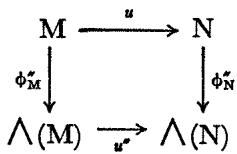
\includegraphics[keepaspectratio]{images/part003_b216bf24.jpg}}

是交换的。此外， \(u''\) 是一个分次代数同态。

\(u''\) 的存在性与唯一性由第 1 号，命题 1 应用于代数 \(\bigwedge(\mathbf{N})\) 和 \(f = \phi_{\mathbf{N}}'' \circ u: \mathbf{M} \to \bigwedge(\mathbf{N})\) 得出；因为 \(f(\mathbf{M}) \subset \mathbf{N}\) ，因此 \(f\) 由 \(\mathfrak{J}_{\mathbf{N}}''\) 的定义满足条件 (1)：由于 \(f(\mathbf{M}) \subset \bigwedge^{1}(\mathbf{N}) = \mathbf{N}\) ，\(u''\) 是分次代数同态这一事实由第 1 号的注记 1 得出。

命题 2 中的同态 \(u''\) 此后将记为 \(\bigwedge(u)\) 。若 P 是一个 A-模且 \(v: \mathbf{N} \to \mathbf{P}\) 是一个 A-线性映射，则

\[
\bigwedge (v \circ u) = \bigwedge (v) \circ \bigwedge (u)\tag{3}
\]

因为 \(\bigwedge(v) \circ \bigwedge(u)\) 是一个代数同态，它使下图交换

\pandocbounded{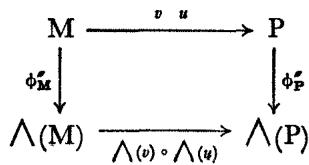
\includegraphics[keepaspectratio]{images/part003_3a522f8d.jpg}}

由于 \(\bigwedge (\mathbf{M})\) 包含 \(\mathbf{M} = \bigwedge^{1}(\mathbf{M}),\bigwedge (u)\) 有时称为 \(u\) 到 \(\bigwedge (\mathbf{M})\) 的典范扩张。限制 \(\bigwedge^n (u):\bigwedge^n (\mathbf{M})\to \bigwedge^n (\mathbf{N})\) 满足

\[
\bigwedge^ {n} (u) (x _ {1} \land x _ {2} \land \dots \land x _ {n}) = u (x _ {1}) \land u (x _ {2}) \land \dots \land u (x _ {n})\tag{4}
\]

（其中 \(x_{i}\in\mathbf{M}\) ），因为 \(\bigwedge(u)\) 是一个代数同态且 \(\bigwedge^{1}(u)=u\) ；限制 \(\bigwedge^{0}(u)\) 在 A 上是恒等映射。注意， \(\bigwedge^{n}(u)\) 是由 \(\mathsf{T}^{n}(u):\mathsf{T}^{n}(\mathbf{M})\to\mathsf{T}^{n}(\mathbf{N})\) 通过过渡到商而得到的。

命题 3. 若 \(u: \mathbf{M} \to \mathbf{N}\) 是满射 A-线性映射，则同态 \(\bigwedge(u): \bigwedge(\mathbf{M}) \to \bigwedge(\mathbf{N})\) 是满射的，且其核为 \(\bigwedge(\mathbf{M})\) 中由核 \(\mathbf{P} \subset \mathbf{M} \subset \bigwedge(\mathbf{M})\) （即 \(u\) 的核）生成的双边理想。

证明由 § 6，第 2 号，命题 4 的证明导出，只需将 S 换为 \(\bigwedge\) 并将 \(\mathfrak{J}'\) 换为 \(\mathfrak{J}''\) 。

若 \(u: \mathbf{M} \to \mathbf{N}\) 是单射线性映射， \(\bigwedge(\mathbf{u})\) 并不总是单射映射（§ 6，练习 3）（然而参见下文第 9 号，命题 12 的推论）。但当 \(u\) 是使得 \(u(\mathbf{M})\) 为 \(\mathbf{N}\) 的直因子的单射时，情况确实如此，且此时 \(\bigwedge(u)\) （同构于 \(\bigwedge(\mathbf{M})\) ）的像是 \(\bigwedge(\mathbf{N})\) 的直因子；其证明与关于 \(\mathbf{T}(u)\) 的类似断言的证明相同（§ 5，第 2 号），只需将 \(\mathbf{T}\) 换为 \(\bigwedge\) 。

命题 4. 设 N 和 P 是 A-模 M 的两个子模，使得它们的和 N + P 是 M 中的直和因子，且它们的交 N ∩ P 是 N 和 P 中的直和因子。则同态 \(\bigwedge(\mathrm{N}) \to \bigwedge(\mathrm{M})\) , \(\bigwedge(\mathrm{P}) \to \bigwedge(\mathrm{M})\) 和 \(\bigwedge(\mathrm{N} \cap \mathrm{P}) \to \bigwedge(\mathrm{M})\) ，即典范单射的典范扩张，是单射；若 \(\bigwedge(\mathrm{N})\) , \(\bigwedge(\mathrm{P})\) 和 \(\bigwedge(\mathrm{N} \cap \mathrm{P})\) 通过这些同态被等同于 \(\bigwedge(\mathrm{M})\) 的子代数，则

\[
\bigwedge (\mathbf {N} \cap \mathbf {P}) = \bigwedge (\mathbf {N}) \cap \bigwedge (\mathbf {P}).\tag{5}
\]

其证明由 § 5，第 2 号，命题 4 的证明导出，只需通篇将 T 换为 \(\bigwedge\) 。当 A 是域时，命题 4 的假设总是被 M 的任意子模 N, P 满足。

推论。设 K 是一个交换域，M 是 K 上的一个向量空间。对每个元素 \(z \in \bigwedge(\mathbf{M})\) ，存在 M 的一个最小向量子空间 N，使得 \(z \in \bigwedge(\mathbf{N})\) 且 N 是有限维的。

证明由 § 5，第 2 号，命题 4 的推论的证明导出，只需通篇将 T 换为 \(\bigwedge\) 。

N 称为 M 的与 \(\bigwedge(\mathbf{M})\) 的元素 z 相关联的向量子空间。
% semantic-fragments: legacy-input-seam
\relax{}
\subsection{外代数的反交换性}

命题5. (i) 设 \((x_{i})_{1\leqslant i\leqslant n}\) 为模 \(\mathbf{M}\) 的元素组成的有限序列；对于每个置换 \(\sigma\) （对称群 \(\mathfrak{S}_n\) 中的），

\[
x _ {\sigma (1)} \wedge x _ {\sigma (2)} \wedge \dots \wedge x _ {\sigma (n)} = \varepsilon_ {\sigma}. x _ {1} \wedge x _ {2} \wedge \dots \wedge x _ {n}\tag{6}
\]

其中 \(\varepsilon_{\sigma}\) 表示置换 \(\sigma\) 的符号。

\begin{enumerate}
\def\labelenumi{(\roman{enumi})}
\setcounter{enumi}{1}
\tightlist
\item
  如果存在两个不同的指标 \(i, j\) 使得 \(x_{i} = x_{j}\) ，则乘积
\end{enumerate}

\[
x _ {1} \wedge x _ {2} \wedge \dots \wedge x _ {n}
\]

为零。

\begin{enumerate}
\def\labelenumi{(\roman{enumi})}
\tightlist
\item
  首先，由于 \(x \wedge x = 0\) 对所有 \(x \in \mathbf{M}\) 成立（由理想 \(\mathfrak{J}''\) 的定义可知），此外，对于 \(x, y\) 属于 \(\mathbf{M}\) 的情形，
\end{enumerate}

\[
x \wedge y + y \wedge x = (x + y) \wedge (x + y) - x \wedge x - y \wedge y = 0.
\]

这确立了（6）在 \(n = 2\) 的情形。一般情形随后由 §4 第 6 号的引理 3 得出。

\begin{enumerate}
\def\labelenumi{(\roman{enumi})}
\setcounter{enumi}{1}
\tightlist
\item
  在 (ii) 的假设下，存在一个置换 \(\sigma \in \mathfrak{S}_n\) ，使得 \(\sigma(1) = i\) 和 \(\sigma(2) = j\) ；那么对这个置换而言，(6) 的左边为零，因此右边也为零。
\end{enumerate}

推论 1. 设 H, K 为 N 的区间 \([1, n]\) 的两个互补子集，并设 \((i_{h})_{1 \leqslant h \leqslant p}, (j_{k})_{1 \leqslant k \leqslant n - p}\) 分别按递增顺序排列的 H 和 K 的元素序列；我们记

\[
x _ {H} = x _ {i _ {1}} \wedge x _ {i _ {2}} \wedge \dots \wedge x _ {i _ {p}}, \quad x _ {K} = x _ {j _ {1}} \wedge x _ {j _ {2}} \wedge \dots \wedge x _ {j _ {n - p}};
\]

那么

\[
x _ {\mathrm{H}} \wedge x _ {\mathrm{K}} = (- 1) ^ {\nu} x _ {1} \wedge x _ {2} \wedge \dots \wedge x _ {n}\tag{7}
\]

其中 \(\nu\) 是有序对 \((i,j)\in \mathbf{H}\times \mathbf{K}\) 中满足 \(i > j\) 者的个数

根据命题5，这归结为证明

引理 1. 若 \(\sigma \in \mathfrak{S}_n\) 是满足 \(\sigma(h) = i_h\) （对 \(1 \leqslant h \leqslant p\) ）与 \(\sigma(h) = j_{h-p}\) （对 \(p + 1 \leqslant h \leqslant n\) ）的置换，则 \(\varepsilon_\sigma = (-1)^{\nu}\) .

对于 \(1 \leqslant h < h' \leqslant p\) 或 \(p + 1 \leqslant h < h' \leqslant n\) ，有 \(\sigma(h') > \sigma(h)\) ，而有序对 \((h, h')\) ——即满足 \(1 \leqslant h \leqslant p < h' \leqslant n\) 与 \(\sigma(h) > \sigma(h')\) 者——的个数等于 \(\nu\) .

推论 2. 分次代数 \(\bigwedge (\mathbf{M})\) 是交错的（§ 4，第 9 号）。

只需将 §4 第 9 号的命题 13 应用于 \(\bigwedge (\mathbf{M})\) ，取生成系为集合 \(\mathbf{M}\) 并利用命题5。

命题6. 若 M 是有限生成的 A-模，则 \(\bigwedge (\mathbf{M})\) 是有限生成的 A-模；此外，若 M 具有含 \(n\) 个元素的生成系，则 \(\bigwedge^{p}(\mathbf{M}) = \{0\}\) 对于 \(p > n\) .

设 \((x_{i})_{1\leqslant i\leqslant n}\) 为 M 的一个生成系。\(\bigwedge^{p}(\mathbf{M})\) 中的每个元素都是形如

\[
x _ {i _ {1}} \wedge x _ {i _ {2}} \wedge \dots \wedge x _ {i _ {p}}
\]

其中指标 \(i_k\) 属于 \([1, n]\) ；根据命题 5，可设这些指标互不相同（否则相应的元素为零）。如果 \(p > n\) ，则不存在这样的指标序列，因此 \(\bigwedge^p(\mathbf{M}) = \{0\}\) 。若 \(p \leqslant n\) ，这样的序列只有有限多个，这就完成了证明。

\subsection{模的n次外幂与交错多重线性映射}

给定交换环 A 上的两个模 M、N，从 \(M^{n}\) 到 N 的交错 n-线性映射是指这样的 n-线性映射 \(f: M^{n} \to N\) ：对所有 \(p \leqslant n - 2\) ，

\[
f (u _ {1}, \dots , u _ {p}, x, x, v _ {1}, \dots , v _ {n - p - 2}) = 0\tag{8}
\]

对所有 \(x\) ，所有 \(u_{i}\) ( \(1 \leqslant i \leqslant p\) ) 以及所有 \(v_{j}\) ( \(1 \leqslant j \leqslant n - p - 2\) ) 在 \(\mathbf{M}\) 中均成立。

命题7. 设 A 为交换环，M 和 N 为两个 A-模。若对每个 A-线性映射 \(g: \bigwedge^n (\mathbf{M}) \to \mathbf{N} (n \geqslant 2)\) 使之对应于 n-线性映射

\[
\left(x _ {1}, x _ {2}, \dots , x _ {n}\right) \mapsto g \left(x _ {1} \wedge x _ {2} \wedge \dots \wedge x _ {n}\right)\tag{9}
\]

便得到从 A-模 \(\operatorname{Hom}_{\mathbf{A}}(\bigwedge^{n}(\mathbf{M}), \mathbf{N})\) 到由交错 \(n\) -线性映射（从 \(\mathbf{M}^n\) 到 \(\mathbf{N}\) 的）所组成的 A-模上的一个双射 A-线性映射。

我们考虑 A-模 \(\operatorname{Hom}_{\mathbf{A}}(\mathsf{T}^{n}(\mathbf{M}),\mathbf{N})\) 到 A-模 \(\mathcal{L}_{n}(\mathbf{M},\ldots,\mathbf{M};\mathbf{N})\) （即所有从 \(M^{n}\) 到 N 的 n-线性映射组成的 A-模）的典范双射，它通过将每个 A-线性映射 \(f: T^{n}(\mathbf{M}) \to \mathbf{N}\) 对应于 n-线性映射而得到

\[
\bar {f} \colon (x _ {1}, \dots , x _ {n}) \mapsto f (x _ {1} \otimes x _ {2} \otimes \dots \otimes x _ {n})
\]

(II, § 3, no. 9)。另一方面，A-线性映射 \(g \colon \bigwedge^{n}(\mathbf{M}) \to \mathbf{N}\) 与 A-线性映射 \(f \colon \mathsf{T}^n (\mathbf{M}) \to \mathbf{N}\) （满足 \(f\) 在 \(\mathfrak{J}_n''\) 上为零者）一一对应，其对应方式是把 \(g\) 映为 \(f = g \circ p_n\) ，其中

\[
p _ {n} \colon \mathsf {T} ^ {n} (\mathbf {M}) \rightarrow \bigwedge^ {n} (\mathbf {M}) = \mathsf {T} ^ {n} (\mathbf {M}) / \mathfrak {J} _ {n} ^ {\prime \prime}
\]

是典范同态（II，§2，第 1 号，定理 1）。但鉴于 \(\mathfrak{J}_n''\) 是形如

\[
\left(u _ {1} \otimes u _ {2} \otimes \dots \otimes u _ {p}\right) \otimes (x \otimes x) \otimes \left(v _ {1} \otimes \dots \otimes v _ {n - p - 2}\right)
\]

\((x, u_{i}, v_{j} \text{ 属于 M}), \text{ 说 } f \text{ 具有形式 } g \circ p_{n} \text{ 意味着相应的 } n\text{-线性函数 } \bar{f} \text{ 满足 (8)，换言之它是交错的。}\)

A-模 \(\bigwedge^{n}(\mathbf{M})\) 称为 \(n\) -次外幂（即 \(\mathbf{M}\) 的外幂）。对于每个 A-模同态 \(u: \mathbf{M} \to \mathbf{N}\) ，映射

\[
\bigwedge^ {n} (u): \bigwedge^ {n} (\mathbf {M}) \rightarrow \bigwedge^ {n} (\mathbf {N})
\]

它与 \(\bigwedge(u)\) 在 \(\bigwedge^{n}(\mathbf{M})\) 上的限制相一致，称为 \(n\) -次外幂（即 \(u\) 的外幂）.

推论 1. 对于每个交错 \(n\) -线性映射 \(g: \mathbf{M}^n \to \mathbf{N}\) ，对于每个置换 \(\sigma \in \mathfrak{S}_n\) ,

\[
g \left(x _ {\sigma (1)}, x _ {\sigma (2)}, \dots , x _ {\sigma (n)}\right) = \varepsilon_ {\sigma}. g \left(x _ {1}, x _ {2}, \dots , x _ {n}\right)\tag{10}
\]

对所有 \(x_{i} \in \mathbf{M}\) 成立；此外，若 \(x_{i} = x_{j}\) 对于两个不同的指标 \(i, j\) 成立，则

\[
g (x _ {1}, x _ {2}, \dots , x _ {n}) = 0.
\]

这是命题 7 以及第 3 号命题 5 的明显推论。

推论2. 设 \((x_{i})_{1\leqslant i\leqslant n}\) 是由 \(n\) 个元素组成的一个序列（元素属于 \(\mathbf{M}\) ），使得

\[
x _ {1} \wedge x _ {2} \wedge \dots \wedge x _ {n} = 0;
\]

那么，对于每一个交错的 \(n\) -线性映射 \(g: \mathbf{M}^n \to \mathbf{N}\) , \(g(x_1, \ldots, x_n) = 0\) .

推论3. 设 \(f: \mathbf{M}^{n-1} \to \mathbf{A}\) 是一个交错 \((n-1)\) -线性形式。如果 \((x_i)_{1 \leq i \leq n}\) 是由 \(n\) 个元素组成的一个序列（元素属于 \(\mathbf{M}\) ），使得 \(x_1 \wedge x_2 \wedge \cdots \wedge x_n = 0\) ，则

\[
\sum_ {i = 1} ^ {n} (- 1) ^ {i} f (x _ {1}, \dots , \hat {x _ {i}}, \dots , x _ {n}). x _ {i} = 0\tag{11}
\]

（其中我们记 \(f(x_{1},\ldots ,\hat{x}_{i},\ldots ,x_{n}) = f(x_{1},\ldots ,x_{i - 1},x_{i + 1},\ldots ,x_{n})\) 对于 \(1\leqslant i\leqslant n\) .

只需证明这个 n-线性映射

\[
(x _ {1}, \dots , x _ {n}) \mapsto \sum_ {i = 1} ^ {n} (- 1) ^ {i} f (x _ {1}, \dots , \hat {x} _ {i}, \dots , x _ {n}). x _ {i}
\]

从 \(M^{n}\) 到 M 是交错的。现在，若 \(x_{i} = x_{i+1}\) ，则由于 f 是交错的，右端求和中除 \(x_{i}\) 与 \(x_{i+1}\) 外的所有项系数均为零；另一方面， \(x_{i}\) 的系数是

\[
(- 1) ^ {i} f (x _ {1}, \dots , x _ {i - 1}, x _ {i + 1}, x _ {i + 2}, \dots , x _ {n})
\]

而 \(x_{i+1}\) 的系数是 \((-1)^{i+1}f(x_1, \ldots, x_i, x_{i+2}, \ldots, x_n)\) ，由假设二者互为相反数。

注记。一个元素 \(z\) 在 \(\mathsf{T}^n (\mathbf{M})\) 中称为 \(n\) 阶（逆变）反对称张量，若 \(\sigma .z = \varepsilon_{\sigma}z\) （对每个置换 \(\sigma \in \mathfrak{S}_n\) ；参见 §6，第 3 号，注记）；这些元素构成一个子 A-模 \(\mathsf{A}_n^\prime (\mathbf{M})\) ，它包含于 \(\mathsf{T}^n (\mathbf{M})\) 。对于所有 \(z\in \mathsf{T}^n (\mathbf{M})\) ，我们记 \(\pmb {a}.z = \sum_{\sigma \in \mathfrak{S}_n}\varepsilon_\sigma (\sigma .z)\) ，并称 \(\pmb {a}.z\) 为 \(z\) 的反对称化；由于 \(\varepsilon_{\sigma \tau} = \varepsilon_{\sigma}\varepsilon_{\tau}\) ，立即可见 \(\pmb {a}.z\) 是反对称张量，因而 \(z\mapsto \pmb {a}.z\) 是 \(\mathsf{T}^n (\mathbf{M})\) 的一个自同态，其像 \(\mathsf{A}_n''(\mathbf{M})\) 包含于 \(\mathsf{A}_n^\prime (\mathbf{M})\) ；一般地 \(\mathsf{A}_n''(\mathbf{M})\neq \mathsf{A}_n^\prime (\mathbf{M})\) （习题 8）。若 \(z\) 是反对称张量，则 \(\pmb {a}.z = n!z\) ；因此，当 \(n!\) 在 A 中可逆时，自同态 \(z\mapsto (n!)^{-1}\pmb {a}.z\) 是 \(\mathsf{T}^n (\mathbf{M})\) 的一个投影算子，其像为

\[
\mathbf {A} _ {n} ^ {\prime} (\mathbf {M}) = \mathbf {A} _ {n} ^ {\prime \prime} (\mathbf {M}).
\]

此外，这个投影算子的核正是 \(\mathfrak{J}_n''\) ；因为显然只需限于 \(n \geqslant 2\) 的情形，于是 2（它是 \(n!\) 的因子）在 A 中可逆，且 \(x \otimes x = 2^{-1}(x \otimes x + x \otimes x)\) ；因此 \(\mathfrak{J}_n''\) 由元素 \(z + \rho . z\) 生成，其中 \(\rho\) 是交换 \([1, n]\) 中两个相邻数的对换；此外，对于两个置换 \(\sigma, \tau\) （在 \(\mathfrak{S}_n\) 中），我们可以写成

\[
z - \varepsilon_ {\sigma \tau} ((\sigma \tau). z) = z - \varepsilon_ {\tau} (\tau . z) + \varepsilon_ {\tau} (\tau . z - \varepsilon_ {\sigma} \sigma . (\tau . z))
\]

由此可得 \(z - \varepsilon_{\sigma}(\sigma . z) \in \mathfrak{J}_{n}^{\prime \prime}\) 对所有 \(z \in \mathbf{T}^{n}(\mathbf{M})\) 和 \(\sigma \in \mathfrak{S}_{n}\) 成立。因此（始终假设 \(n!\) 在 A 中可逆），可以看出

\[
z - (n!) ^ {- 1} \boldsymbol {a}. z = \sum_ {\sigma \in \mathfrak {S} _ {n}} (n!) ^ {- 1} (z - \varepsilon_ {\sigma} (\sigma . z)) \in \mathfrak {J} _ {n} ^ {\prime \prime}
\]

对所有 \(z \in \mathbf{T}^n(\mathbf{M})\) 成立，这确立了我们的断言。

当 \(n!\) 在 A 中可逆时，子模 \(\mathsf{A}_n'(M)\) 和 \(\mathfrak{J}_n''\) （均为 \(T^n(M)\) 的子模）因此是互补的，并且限制到 \(\mathsf{A}_n'(M)\) 上的典范同态 \(T^n(M) \to \bigwedge^n(M) = T^n(M)/\mathfrak{J}_n''\) 是一个 A-模同构，这使我们在所讨论的情形下可以把 \(n\) 阶反对称张量与 M 的 \(n\) -次外幂的元素等同起来。这里还需注意，这一等同与乘法不相容：两个反对称张量在 \(T(M)\) 中的乘积一般不再是反对称的。

\subsection{标量环的扩张}

设 A, A' 为两个交换环， \(\rho:A\to A'\) 为环同态，M 为 A-模，M' 为 A'-模，且 \(f:M\to M'\) 为从 M 到 M' 的 A-同态（相对于 \(\rho\) ）。复合映射 \(M\xrightarrow{f}M'\xrightarrow{\phi_{M'}^{\prime\prime}}\bigwedge_{A'(M')}\) 是从 M 到 A-代数 \(\bigwedge_{A'(M')}\) 的 A-线性映射，并且，由于 \(f(\mathbf{M}) \subset \mathbf{M}'\) 的元素在 \(\bigwedge_{\mathbf{A}'}(\mathbf{M}')\) 中平方为零，存在（第 1 号，命题 1）一个且仅一个代数的 A-同态 \(f'': \bigwedge_{\mathbf{A}}(\mathbf{M}) \to \bigwedge_{\mathbf{A}'}(\mathbf{M}')\) 使图表交换

\begin{enumerate}
\def\labelenumi{(\arabic{enumi})}
\setcounter{enumi}{11}
\tightlist
\item
\end{enumerate}

\pandocbounded{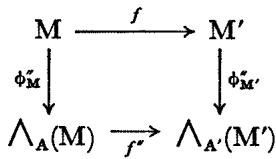
\includegraphics[keepaspectratio]{images/part003_899f4c21.jpg}}

和 \(f''\) 是分次代数同态。立即可以推出，如果 \(\sigma: A' \to A''\) 是另一个环同态， \(M''\) 一个 \(A''\) -模， \(g: M' \to M''\) 一个 \(A'\) -同态（相对于 \(\sigma\) ) 且 \(g'': \bigwedge_{A'}(M') \to \bigwedge_{A''}(M'')\) 相应的 \(A''\) -代数的同态，则复合的代数 A-同态

\[
\bigwedge_ {\mathbf {A}} (\mathbf {M}) \xrightarrow {f ^ {\prime \prime}} \bigwedge_ {\mathbf {A} ^ {\prime}} (\mathbf {M} ^ {\prime}) \xrightarrow {g ^ {\prime \prime}} \bigwedge_ {\mathbf {A} ^ {\prime \prime}} (\mathbf {M} ^ {\prime \prime})\tag{13}
\]

对应于复合 A-同态 \(g \circ f: \mathbf{M} \to \mathbf{M}''\) （相对于 \(\sigma \circ \rho\) ）。

命题 8. 设 A、B 为两个交换环， \(\rho: A \to B\) 一个环同态，且 M 是一个 A-模。典范扩张

\[
\psi : \bigwedge_ {\mathbf {B}} (\mathbf {B} \otimes_ {\mathbf {A}} \mathbf {M}) \rightarrow \mathbf {B} \otimes_ {\mathbf {A}} \bigwedge_ {\mathbf {A}} (\mathbf {M})
\]

的典范扩张是一个分次 B-代数同构，这里所指的 B-线性映射是 \(l_{B} \otimes \phi_{M}^{\prime\prime}: B \otimes_{A} M \to B \otimes_{A} \bigwedge_{A}(M)\) 。

证明源自 §5 第 4 号命题 5 的证明，只需将 T 换为 \(\bigwedge\) ，并将 \(\phi_{\mathbf{M}}\) 换为 \(\phi_{\mathbf{M}}^{\prime \prime}\) 。

\subsection{外代数的正向极限}

设 \((\mathbf{A}_{\alpha},\phi_{\beta \alpha})\) 为交换环的一个有向正向系统， \((\mathbf{M}_{\alpha},f_{\beta \alpha})\) 为 \(\mathbf{A}_{\alpha}\) -模的一个正向系统， \(\mathbf{A} = \varinjlim \mathbf{A}_{\alpha}\) 与 \(\mathbf{M} = \varinjlim \mathbf{M}_{\alpha}\) 。对于 \(\alpha \leqslant \beta\) ，我们由 \(\mathbf{A}_{\alpha}\) -同态 \(f_{\beta \alpha}: \overrightarrow{\mathbf{M}_{\alpha}} \to \mathbf{M}_{\beta}\) 典范地导出一个 \(\mathbf{A}_{\alpha}\) -代数同态（第 5 号，公式 (12)） \(f_{\beta \alpha}^{\prime \prime}: \bigwedge_{\mathbf{A}_{\alpha}} (\mathbf{M}_{\alpha}) \to \bigwedge_{\mathbf{A}_{\beta}} (\mathbf{M}_{\beta})\) ，并且由 (13) 可知 \((\bigwedge_{\mathbf{A}_{\alpha}} (\mathbf{M}_{\alpha}), f_{\beta \alpha}^{\prime \prime})\) 是分次 \(\mathbf{A}_{\alpha}\) -模的一个正向系统。另一方面，设 \(f_{\alpha}: \mathbf{M}_{\alpha} \to \mathbf{M}\) 为典范 \(\mathbf{A}_{\alpha}\) -同态；我们（由第 5 号，公式 (12)）导出一个分次 \(\mathbf{A}_{\alpha}\) -代数同态 \(f_{\alpha}^{\prime \prime}: \bigwedge_{\mathbf{A}_{\alpha}} (\mathbf{M}_{\alpha}) \to \bigwedge_{\mathbf{A}} (\mathbf{M})\) ，并且由 (13) 同样得出 \(f_{\alpha}^{\prime \prime}\) 构成 \(\mathbf{A}_{\alpha}\) -同态的一个正向系统。

命题9. A-同态 \(f'' = \varinjlim f_{\alpha}' : \varinjlim \bigwedge_{A_{\alpha}}(M_{\alpha}) \to \bigwedge_{A}(M)\) 是一个分次代数同构。

证明与 §5 第 4 号命题 6 的证明相同，只需将其中所有的 T 换为 \(\bigwedge\) ，将 \(\phi\) 换为 \(\phi''\) ，并注意到交错代数的正向极限仍是交错的。

\subsection{直和的外代数。分次模的外代数}

设 A 为一个交换环， \(M = \bigoplus_{\lambda \in L} M_{\lambda}\) 为一族 A-模的直和，以及 \(j_{\lambda}: M_{\lambda} \to M\) 为典范单射；由此导出一个分次代数的 A-同态 \(\bigwedge(j_{\lambda}): \bigwedge(M_{\lambda}) \to \bigwedge(M)\) 。由于 \(\bigwedge(M)\) 是反交换的，§4 第 7 号命题 10（或在必要时推广到 L 为无限的情形，参见 §4 第 8 号注记 1）可应用于同态 \(\bigwedge(j_{\lambda})\) ；则存在唯一的代数同态

\[
g \colon \bigotimes_ {\lambda \in L} ^ {g} \Lambda (M _ {\lambda}) \to \Lambda (M)\tag{14}
\]

（也记作 \(g_{\mathbf{M}}\) ）使得 \(\bigwedge (j_{\lambda}) = g \circ f_{\lambda}\) ，其中

\[
f _ {\lambda}: \bigwedge (\mathrm{M} _ {\lambda}) \rightarrow \bigotimes_ {\lambda \in L} ^ {g} \bigwedge (\mathrm{M} _ {\lambda})
\]

表示典范同态。

命题10. 典范同态 \(g\) （公式（14））是分次代数同构。

为了证明 \(g\) 是双射，我们定义一个分次代数同态

\[
h: \bigwedge (\mathbf {M}) \rightarrow \bigotimes_ {\lambda \in L} ^ {\mathfrak {g}} \bigwedge (\mathbf {M} _ {\lambda})\tag{15}
\]

使得 \(g \circ h\) 与 \(h \circ g\) 分别是 \(\bigwedge(\mathbf{M})\) 与 \(\bigotimes_{\lambda \in L} \bigwedge(\mathbf{M}_{\lambda})\) 上的恒等映射。对于每个 \(\lambda \in L\) ，考虑复合线性映射

\[
u _ {\lambda}: \mathrm{M} _ {\lambda} \xrightarrow {\phi_ {\mathrm{M} _ {\lambda}} ^ {n}} \bigwedge (\mathrm{M} _ {\lambda}) \xrightarrow {f _ {\lambda}} \mathbf {g} _ {\lambda \in L} \bigotimes \bigwedge (\mathrm{M} _ {\lambda}).
\]

存在且仅存在一个 A-线性映射 \(u: \mathbf{M} \to {}^{\mathfrak{g}} \bigotimes_{\lambda \in L} \bigwedge (\mathbf{M}_{\lambda})\) ，使得 \(u \circ j_{\lambda} = u_{\lambda}\) （对所有 \(\lambda \in L\) ）。斜张量积 \({}^{\mathfrak{g}} \bigotimes_{\lambda \in L} \bigwedge (\mathbf{M}_{\lambda})\) 是一个交错代数：当 L 有限时，这由 §4 第 9 号命题 14 得出；当 L 任意时，这由 §4 第 8 号注记 1 中给出的该乘积的定义以及交错分次代数的正向极限是交错的这一事实得出。由于 \(u(\mathbf{M})\) 也包含在分次代数 \(\bigotimes_{\lambda \in L} \bigwedge (\mathbf{M}_{\lambda})\) 中次数为1的元素子模中，由第1号命题1和注记1可知，存在唯一的分次代数同态。

\[
h: \bigwedge (\mathbf {M}) \rightarrow \bigotimes_ {\lambda \in L} ^ {\mathfrak {g}} \bigwedge (\mathbf {M} _ {\lambda})
\]

使得 \(h \circ \phi_{\mathbf{M}}'' = u\) 。 \(g \circ h\) 与 \(h \circ g\) 为恒等映射这一事实的验证，与 §6 第 6 号命题 9 中的做法相同，只需将 \(\mathbf{S}\) 换为 \(\bigwedge\) ，将 \(\phi'\) 换为 \(\phi''\) 。

注记。设 \(N = \bigoplus_{\lambda \in L} N_{\lambda}\) 为以 L 为指标集的另一族 A-模的直和，并且对所有 \(\lambda \in L\) ，设 \(v_{\lambda}: M_{\lambda} \to N_{\lambda}\) 为一个 A-线性映射，于是存在 A-线性映射 \(v = \bigoplus_{\lambda} v_{\lambda}: M \to N\) （II，§1，第 6 号，命题 7）。则图表

\[
\begin{array}{c c c} \mathbf {g} _ {\lambda \in L} ^ {\otimes} \wedge (\mathrm{M} _ {\lambda}) & \xrightarrow {g _ {\mathrm{M}}} & \wedge (\mathrm{M}) \\ \bigotimes_ {\lambda \in L} \wedge (v _ {\lambda}) \Big \downarrow & & \Big \downarrow \wedge (v) \\ \mathbf {g} _ {\lambda \in L} ^ {\otimes} \wedge (\mathrm{N} _ {\lambda}) & \xrightarrow {g _ {\mathrm{N}}} & \wedge (\mathrm{N}) \end{array}
\]

是交换的（参见第4节第5号命题8的推论）。

\(\mathbf{g}_{\lambda \in L}^{\otimes} \bigwedge (\mathbf{M}_{\lambda})\) 的 A-子模（ \(\bigwedge^{n}(\mathbf{M})\) 借助同构 \(g\) 与之等同者）可以得到更精确的描述。对每个有限子集 \(J\) （ \(L\) 的），我们记 \(\mathrm{E}_{J} = \mathbf{g}_{\lambda \in J}^{\otimes} \bigwedge (\mathbf{M}_{\lambda})\) ，从而 \(\mathbf{g}_{\lambda \in L}^{\otimes} \bigwedge (\mathbf{M}_{\lambda}) = \lim_{\lambda \to 0} \mathrm{E}_{J}\) 相对于有向集 \(\mathfrak{F}(L)\) （ \(L\) 的有限子集组成的）成立，这是依据定义（§ 4，第 8 号，注记 1）。对每个族 \(\nu = (n_{\lambda}) \in \mathbf{N}^{(L)}\) （从而具有有限支集），它满足 \(\sum_{\lambda \in L} n_{\lambda} = n\) ；对每个有限子集 \(J\) （ \(L\) 的、包含族 \(\nu\) 的支集者），我们记

\[
\bigwedge^ {J, v} (\mathbf {M}) = \bigotimes_ {\lambda \in J} \bigwedge^ {n _ {\lambda}} (\mathbf {M} _ {\lambda})\tag{16}
\]

使得子模 \(\mathbf{E}_{\mathbf{J},n}\) ——即次数 \(n\) 的元素在 \(\mathbf{E}_{\mathbf{J}}\) 中组成的子模——是诸 \(\bigwedge^{\mathbf{J},\nu}(\mathbf{M})\) 的直和，这里族 \(\nu\) 的支集包含于 \(\mathbf{J}\) 且使得

\[
\sum_ {\lambda \in L} n _ {\lambda} = n
\]

（§ 4，第 7 号，命题 10 及第 8 号）。按约定，我们记 \(\bigwedge^{J,\nu}(\mathbf{M}) = \{0\}\) （对族 \(\nu\) ，其支集不包含于 \(J\) ）；于是

\(E_{J,n}\) 也可称为所有 \(\bigwedge^{J,\nu}(M)\) 的直和，其中 \(\nu\) 遍历集合 \(H_n\) ，即所有族 \(\nu = (n_\lambda)_{\lambda \in L}\) （满足 \(\sum_{\lambda \in L} n_\lambda = n\) 者）组成的集合。由于 \(\bigwedge^0(M_\lambda)\) 与 A 等同，显然对 L 的两个有限子集 \(J \subset J'\) 以及支集包含于 J 的族 \(\nu\) ，典范映射 \(\bigwedge^{J,\nu}(M) \to \bigwedge^{J',\nu}(M)\) （即典范映射 \(E_J \to E_{J'}\) 在 \(\bigwedge^{J,\nu}(M)\) 上的限制）是双射。如果对所有 \(\nu \in H_n\) ，

\[
\bigwedge^ {\nu} (\mathbf {M}) = \varinjlim \bigwedge^ {J, \nu} (\mathbf {M})\tag{17}
\]

于是可见，考虑到 II，§ 6，第 2 号，命题 5，我们有：

推论. A-模 \(\bigwedge^{n}(\mathbf{M})\) 是 \(\bigotimes_{\lambda \in L} \bigwedge (\mathbf{M}_{\lambda})\) 的一个子模在同构 (14) 下的像，该子模是诸子模 \(\bigwedge^{\nu}(\mathbf{M})\) 的直和，其中族 \(\nu = (n_{\lambda}) \in \mathbf{N}^{(L)}\) 满足 \(\sum_{\lambda \in L} n_{\lambda} = n\) ；若 \(J\) 是 \(\nu, \bigwedge^{\nu}(\mathbf{M})\) 的支集，则它典范同构于 \(\bigotimes_{\lambda \in J} \bigwedge^{n_{\lambda}}(\mathbf{M}_{\lambda})\) .

一般将 \(\bigwedge^{\nu}(\mathbf{M}),\bigotimes_{\lambda \in J}\bigwedge^{n_{\lambda}}(\mathbf{M}_{\lambda})\) 与它们在 \(\bigwedge^n (\mathbf{M})\) 中的像等同起来。按此约定：

命题11. 设 \(\Delta\) 为交换幺半群， \(\mathbf{M}\) 为类型 \(\Delta\) 的分次 A-模， \((\mathbf{M}_{\alpha})_{\alpha \in \Delta}\) 为其分次。对于每个有序对 \((\alpha, n) \in \Delta \times \mathbf{N}\) ，设 \(\bigwedge^{\alpha, n}(\mathbf{M})\) 为 \(\bigwedge^n (\mathbf{M})\) 的这样的子模：它是诸子模 \(\bigotimes_{\lambda \in J} \bigwedge^{n_{\lambda}}(\mathbf{M}_{\alpha_{\lambda}})\) 的直和，其中 \((n_{\lambda})_{\lambda \in L}\) 遍历整数 \(\geqslant 0\) 的、满足 \(\sum_{\lambda \in L} n_{\lambda} = n\) 的族所成的集合， \(J\) 为其支集，且对于每个 \((n_{\lambda})\) , \((\alpha_{\lambda})_{\lambda \in J}\) 遍历 \(\Delta^J\) 中满足 \(\sum_{\lambda \in J} \alpha_{\lambda} = \alpha\) 的族所成的集合。则 \((\bigwedge^{\alpha, n}(\mathbf{M}))_{(\alpha, n) \in \Delta \times N}\) 是唯一的类型为 \(\Delta \times N\) 、与 \(\bigwedge(\mathbf{M})\) 上的代数结构相容并且在 \(\mathbf{M} = \bigwedge^1 (\mathbf{M})\) 上诱导出给定分次的分次。

\(\bigwedge (\mathbf{M})\) 是诸 \(\bigwedge^{\alpha ,n}(\mathbf{M})\) 的直和这一事实由命题 10 的推论得出；证明的其余部分与 §5 第 5 号命题 7 的证明结尾完全相同。

\subsection{自由模的外代数}

定理1. 设M是一个具有基的A-模 \((e_{\lambda})_{\lambda \in L}\) 。设 L 被赋予全序集的结构（集合论，III，§2，第 3 号，定理 1），并且对于 L 的每个有限子集 J，我们记

\[
e _ {J} = e _ {\lambda_ {1}} \wedge e _ {\lambda_ {2}} \wedge \dots \wedge e _ {\lambda_ {n}}\tag{18}
\]

（其中 \((\lambda_k)_{1 \leqslant k \leqslant n}\) 是 \(J\) 的元素按递增顺序排列的序列（集合论，III，§5，第 3 号，命题 6）；我们记 \(e_\varphi = 1\) ，即 A 的单位元。则诸 \(e_J\) （其中 \(J\) 遍历有限子集组成的集合 \(\mathfrak{F}(L)\) （ \(L\) 的））构成外代数 \(\bigwedge(M)\) 的一组基。

由于 \(e_{\lambda}\) 生成 A-模 M， \(\bigwedge(\mathbf{M})\) 的每个元素都是有限个 \(e_{\lambda}\) 之乘积的线性组合，从而（考虑到第 3 号命题 5）是有限个元素 \(e_{J}\) （ \(J \in \mathfrak{F}(L)\) ）的线性组合。剩下要证明 \(e_{J}\) 在 A 上线性无关。否则，这些元素之间将存在一个系数不全为零的线性关系；此关系中诸 \(e_{J}\) （其系数 \(\neq 0\) 者）所对应的子集 J 的并是 L 的一个有限子集 K（因为系数 \(\neq 0\) 的只有有限个）。设 N 为 M 的由诸 \(e_{\lambda}\) （满足 \(\lambda \in K\) 者）生成的子模；N 是 M 的一个直因子，因此（第 2 号） \(\bigwedge(\mathbf{N})\) 等同于 \(\bigwedge(\mathbf{M})\) 的一个子代数，并且，如果我们证明诸 \(e_{J}\) （ \(J \subset K\) ）构成 \(\bigwedge(\mathbf{N})\) 的一组基，我们将得到所期望的矛盾。

因此，问题归结为在 M 的基为有限时证明定理 1；于是我们可以假设 \(L = [1, m] \subset N\) 。对于每个 \(i \in L\) ，设 \(M_i\) 为 M 的自由子模 \(Ae_i\) ；M 是诸 \(M_i\) 的直和，而 \(\bigwedge(M_i)\) 是 \(\bigwedge^0(M_i) = A\) 与 \(\bigwedge^1(M_i) = M_i\) （第 3 号，命题 6）的直和。令 \(\bigwedge(M)\) 与诸 \(\bigwedge(M_i)\) 的张量积这一 A-模（第 7 号，命题 10）典范地等同；后者以诸基 \((1, e_i)\) （诸 \(\bigwedge(M_i)\) 的基）的张量积为基（II，§ 3，第 7 号，命题 7 的推论 2）；因此我们得到所有元素

\[
u _ {1} \otimes u _ {2} \otimes \dots \otimes u _ {m}
\]

其中 \(u_{i}=1\) 或 \(u_{i}=e_{i}\) ；若 J 是使得 \(u_{i}=e_{i}\) 的指标 i 组成的集合，则 \(u_{1}\otimes u_{2}\otimes\cdots\otimes u_{m}\) 与 \(e_{J}\) 等同，这就完成了证明。

推论 1. 假设 \(\mathbf{L} = [1, m]\) ；则基 \((e_{\mathrm{J}})_{\mathrm{J} \in \mathfrak{P}(\mathrm{L})}\) （ \(\bigwedge (\mathbf{M})\) 的）有 \(2^{m}\) 个元素。对于 \(p > m\) , \(\bigwedge^{p}(\mathbf{M}) = \{0\}\) ； \(\bigwedge^{m}(\mathbf{M})\) 有由单个元素 \(e_{\mathrm{L}}\) 组成的基；对于 \(0 \leqslant p \leqslant m\) ，基 \((e_{\mathrm{J}})\) （ \(\bigwedge^{p}(\mathbf{M})\) 的、由诸 \(e_{\mathrm{J}}\) （满足 \(\operatorname{Card}(\mathbf{J}) = p\) 者）组成的）的元素个数是

\[
\binom {m} {p} = \frac {m !}{p ! (m - p) !}.
\]

这可由《集合论》III，§3，第5号，命题12以及《集合论》III，§5，第8号，命题11的推论1得出。

我们回到定理 1 中集合 L 为任意的情形，并明确给出基 \((e_{J})\) 的乘法表（§1，第 7 号）。给定两个有限子集 \(J\) , \(K\) （全序集 \(L\) 的），我们记

\[
\left\{ \begin{array}{l l} \rho_ {J, K} = 0 & \text { if } J \cap K \neq \varnothing \\ \rho_ {J, K} = (- 1) ^ {\nu} & \text { if } J \cap K = \varnothing \end{array} \right.\tag{19}
\]

其中 v 表示有序对 \((\lambda, \mu) \in J \times K\) 中满足 \(\lambda > \mu\) 者的个数。于是，第 2 号命题 4 的推论 1 立即蕴含关系

\[
e _ {J} \wedge e _ {K} = \rho_ {J, K} e _ {J \cup K}.\tag{20}
\]

注意公式

\[
\rho_ {J, K} \rho_ {K, J} = (- 1) ^ {j k}\tag{21}
\]

当 \(\mathbf{J} \cap \mathbf{K} = \varnothing, j = \operatorname{Card}(\mathbf{J}), k = \operatorname{Card}(\mathbf{K})\) (第3号，命题5之推论2。)

推论2. 若M是投射A-模， \(\bigwedge (\mathbf{M})\) 是投射 A-模。

证明与第5节第5号定理1的推论相同，只需将T替换为 \(\Lambda\) .

推论3. 设 M 为投射 A-模，且 \((x_{i})_{1\leqslant i\leqslant n}\) 为 M 的元素组成的有限序列。要在 M 上存在一个交错 \(n\) -线性形式 \(f\) ，使得

\[
f (x _ {1}, x _ {2}, \dots , x _ {n}) \neq 0,
\]

其充要条件是 \(x_{1} \wedge x_{2} \wedge \cdots \wedge x_{n} \neq 0\) .

我们已经知道（在对 M 不作任何假设的情况下）该条件是必要的（第 4 号，命题 7）。现在假设 M 是投射的，并且

\[
x _ {1} \wedge x _ {2} \wedge \dots \wedge x _ {n} \neq 0.
\]

那么 \(\bigwedge^n (\mathbf{M})\) 是投射的（推论 2），因此典范映射

\[
\bigwedge^ {n} (\mathbf {M}) \rightarrow (\bigwedge^ {n} (\mathbf {M})) ^ {* *}
\]

是单射的（II，§2，第7号，命题13的推论4）；我们由此得出结论，存在一个线性形式 \(g: \bigwedge^{n}(\mathbf{M}) \to \mathbf{A}\) ，使得 \(g(x_{1} \wedge x_{2} \wedge \dots \wedge x_{n}) \neq 0\) 。若 \(f\) 是交错 \(n\) -线性形式中与 \(g\) 相对应的那一个（第 4 号，命题 7），则 \(f(x_{1}, \ldots, x_{n}) \neq 0\) .

\subsection{线性无关的判定准则}

命题12. 设M是一个投射A-模。对于M中的元素 \(x_1, x_2, \ldots, x_n\) 线性相关，必要且充分条件是存在 \(\lambda \neq 0\) ，以及

\[
\lambda x _ {1} \wedge x _ {2} \wedge \dots \wedge x _ {n} = 0.\tag{22}
\]

该条件是必要的（对 M 不作任何假设），因为例如若 \(\lambda x_{1}\) （其中 \(\lambda \neq 0\) ）是 \(x_{2}, \ldots, x_{n}\) 的线性组合，则关系式 (22) 成立（第 3 号，命题 5）。我们通过对 n 作归纳来证明该条件是充分的；对于 n = 1，它是定义的一个平凡推论。因此假设 n \textgreater{} 1 且条件 (22) 对某个 \(\lambda \neq 0\) 成立。若

\[
\lambda x _ {2} \wedge x _ {3} \wedge \dots \wedge x _ {n} = 0,
\]

成立，则归纳假设蕴含 \(x_{2},\ldots,x_{n}\) 线性相关，从而当然 \(x_{1},x_{2},\ldots,x_{n}\) 也线性相关。若 \(\lambda x_{2}\wedge x_{3}\wedge\cdots\wedge x_{n}\neq0\) ，则由第 8 号定理 1 的推论 3 可知，存在一个交错的 \((n-1)\) -线性形式 f 使得 \(f(\lambda x_{2}\wedge x_{3}\wedge\cdots\wedge x_{n})=\mu\neq0\) 。由于

\[
x _ {1} \wedge (\lambda x _ {2}) \wedge \dots \wedge x _ {n} = 0,
\]

由第 8 号定理 1 的推论 3 可知， \(\mu x_{1}\) 是 \(\lambda x_{2}, x_{3}, \ldots, x_{n}\) 的线性组合；因此 \(x_{1}, x_{2}, \ldots, x_{n}\) 线性相关。

推论. 设M和N是两个投射A-模，且 \(f:M\to N\) 是一个A-线性映射。若f是单射，则 \(\bigwedge(f):\bigwedge(\mathbf{M})\to\bigwedge(\mathbf{N})\) 是单射。

我们首先在M是自由的假设下证明这一点；设 \((e_{\lambda})_{\lambda \in L}\) 是M的一组基，从而 \((e_{J})_{J \in \mathfrak{F}(L)}\) （公式(18)）是 \(\bigwedge(M)\) 的一组基。假设 \(\bigwedge(f)\) 的核包含一个元素 \(u = \sum_{J} \alpha_{J} e_{J} \neq 0\) 。设K是使得 \(\alpha_{J} \neq 0\) 的有限子集J中极小者，并设H是L的一个与K不相交的有限子集，使得 \(K \cup H\) 包含所有（有限个）使得 \(\alpha_{J} \neq 0\) 的 J ；于是对所有满足 \(J \neq K\) 且 \(\alpha_{J} \neq 0\) 的 J ，按定义我们有 \(J \cap H \neq 0\) ，从而（第 8 号，公式 (20)）

\[
u \wedge e _ {\mathrm{H}} = + \alpha_ {\mathbf {K}} e _ {\mathbf {K} \cup \mathbf {H}}
\]

属于 \(\bigwedge (\mathbf{M})\) 的双边理想，即 \(\bigwedge (f)\) 的核。我们记 \(e_{\mathbf{K} \cup \mathbf{H}} = e_{\lambda_1} \wedge e_{\lambda_2} \wedge \dots \wedge e_{\lambda_n}\) ；于是 \(\alpha_{\mathbf{K}} f(e_{\lambda_1}) \wedge f(e_{\lambda_2}) \wedge \dots \wedge f(e_{\lambda_n}) = 0\) ；根据命题 12，N 中的元素 \(f(e_{\lambda_i})\) ( \(1 \leqslant i \leqslant n\) ) 线性相关。但这与假设 \(f\) 是单射（II，§1，第11号，命题17的推论3）相矛盾。

现在我们考虑一般情形；设 \(\mathbf{M}'\) 是一个A-模，使得 \(\mathbf{M} \oplus \mathbf{M}' = \mathbf{P}\) 是自由的（II，§2，第2号，命题4）。考虑线性映射 \(g: \mathbf{M} \oplus \mathbf{M}' \to \mathbf{N} \oplus \mathbf{M} \oplus \mathbf{M}'\) ，它使得 \(g(x, y) = (f(x), 0, y)\) ，从而有交换图

\pandocbounded{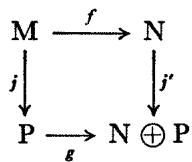
\includegraphics[keepaspectratio]{images/part004_a147f11a.jpg}}

其中竖直箭头是典范单射。由于g是单射且P是自由的， \(\bigwedge(g)\) 如上所见是一个单射同态。现在， \(\bigwedge(j):\bigwedge(\mathbf{M})\to\bigwedge(\mathbf{P})\) 是一个单射同态，因为M是P的一个直因子（第2号）。复合同态

\[
\bigwedge (\mathbf {M}) \xrightarrow {\bigwedge (j)} \bigwedge (\mathbf {P}) \xrightarrow {\bigwedge (g)} \bigwedge (\mathbf {N} \oplus \mathbf {P})
\]

因此是单射的，并且由于它也等于复合同态

\[
\Lambda (\mathbf {M}) \xrightarrow {\Lambda (f)} \Lambda (\mathbf {N}) \xrightarrow {\Lambda (j ^ {\prime})} \Lambda (\mathbf {N} \oplus \mathbf {P})
\]

我们得出结论 \(\bigwedge (f)\) 是单射。

命题13. 设 M 是一个 A-模，N 是 M 的一个直因子子模，它是维数为 p 的自由模，且 \(\{u\}\) 是 \(\bigwedge^{p}(\mathbf{N})\) 的一组基。对于元素 \(x \in M\) 属于 N，必要且充分条件是 \(u \wedge x = 0\) .

设P是M中与N互补的子模，且设 \(y \in N\) , \(z \in P\) 使得 \(x = y + z\) 。则 \(u \wedge x = u \wedge z\) 。由于 \(\bigwedge^{p}(N)\) 是维数为 1 的自由模，映射 \(\phi: P \to P \otimes \bigwedge^{p}(N)\) （它由 \(\phi(p) = p \otimes u\) 给出）是双射（II，§3，第 4 号，命题 4）。另一方面（第7号，命题10），典范同态的复合

\[
\psi : \mathrm{P} \otimes \bigwedge^ {p} (\mathrm{N}) \rightarrow \bigwedge (\mathrm{P}) \otimes \bigwedge (\mathrm{N}) \rightarrow \bigwedge (\mathrm{M})
\]

是单射的。映射 \(\psi \circ \phi\) 因此是单射的，从而命题得证。

定理2. 设 \(\mathbf{M}\) 是一个具有有限基 \((e_i)_{1\leqslant i\leqslant n}\) 的A-模。对于序列 \((x_i)_{1\leqslant i\leqslant n}\) （ \(n\) 个属于 \(\mathbf{M}\) 的元素）构成 \(\mathbf{M}\) 的一个基，必要且充分条件是使得下式成立的元素 \(\lambda \in \mathbf{A}\)

\[
x _ {1} \wedge x _ {2} \wedge \dots \wedge x _ {n} = \lambda . e _ {1} \wedge e _ {2} \wedge \dots \wedge e _ {n}\tag{23}
\]

在 A 中可逆。

请回忆 \(e_{1} \wedge e_{2} \wedge \cdots \wedge e_{n}\) 是 \(\bigwedge^{n}(\mathbf{M})\) 的一个基中的唯一元素（第 8 号，定理 1 的推论 1），因而满足 (23) 的元素 \(\lambda \in A\) 被唯一确定。若 \((x_{i})_{1 \leqslant i \leqslant n}\) 是 M 的一组基，则 \(x_{1} \wedge x_{2} \wedge \cdots \wedge x_{n}\) 是 \(\bigwedge^{n}(\mathbf{M})\) 的一个基中的唯一元素（第 8 号），于是 \(\lambda\) 是可逆的。反之，假设 \(\lambda\) 是可逆的；那么对应于线性映射 \(g: \bigwedge^{n}(\mathbf{M}) \to \mathbf{A}\) （它使得

\[
g (e _ {1} \wedge e _ {2} \wedge \dots \wedge e _ {n}) = \lambda^ {- 1}
\]

）的交错 n-线性形式 f 满足 \(f(x_{1}, x_{2}, \ldots, x_{n}) = 1\) 。对于所有 \(x \in \mathbf{M}\) ，显然

\[
x \wedge x _ {1} \wedge \dots \wedge x _ {n} = 0
\]

（第 3 号，命题 6）；将第 8 号，定理 1 的推论 3 应用于此，我们得到

\[
f (x _ {1}, x _ {2}, \dots , x _ {n}). x = \sum_ {i = 1} (- 1) ^ {i - 1} f (x, x _ {1}, \dots , \hat {x} _ {i}, \dots , x _ {n}). x _ {i}.
\]

由于 \(f(x_{1},\ldots ,x_{n}) = 1\) ，这表明每一个 \(x\in \mathbf{M}\) 都是 \(x_{1},x_{2},\ldots ,x_{n}\) 的线性组合，且由于它们线性无关（因为

\[
x _ {1} \wedge x _ {2} \wedge \dots \wedge x _ {n} \neq 0),
\]

它们构成M的一组基。

\section{行列式}

\subsection{自同态的行列式}

设 M 是一个具有 n 个元素的有限基的 A-模，u 是 M 的一个自同态。A-模 \(\bigwedge^{n}(\mathbf{M})\) 是一个单生成自由模，即与A同构（第8号，定理1的推论1）。 \(\bigwedge^{n}(u)\) 是该模的一个自同态，因此是一个位似 \(z \mapsto \lambda z\) ，其位似比 \(\lambda \in A\) 被唯一确定（II，§2，第 3 号，命题 5）。

定义 1. 一个自同态 \(u\) （自由 A-模 \(M\) 的、维数 \(n\) 为有限者；II，§7，第 2 号，命题 3 的推论及注记 1）的行列式，记作 \(\det u\) ，是标量 \(\lambda\) （它使得 \(\bigwedge^{n}(u)\) 是比率为 \(\lambda\) 的位似）.

根据 §7 第 2 号的公式 (4)，det u 是使得下式成立的唯一标量：

\[
u \left(x _ {1}\right) \wedge u \left(x _ {2}\right) \wedge \dots \wedge u \left(x _ {n}\right) = (\det u). x _ {1} \wedge x _ {2} \wedge \dots \wedge x _ {n}\tag{1}
\]

对每个序列 \((x_{i})_{1\leqslant i\leqslant n}\) （ \(n\) 个 M 的元素）成立。如果 \(\det (u) = 1\) ，则称 \(u\) 为幺模的。

命题1.（i）若 \(u\) 和 \(v\) 是两个有限维自由A-模M的自同态，则

\[
\det (u \circ v) = (\det u) (\det v).\tag{2}
\]

\begin{enumerate}
\def\labelenumi{(\roman{enumi})}
\setcounter{enumi}{1}
\tightlist
\item
  \(\operatorname{det}(1_{\mathbf{M}}) = 1\) ；对每个自同构 \(u\) （ \(\mathbf{M}\) 的自同构）， \(\operatorname{det} u\) 在 \(\mathbf{A}\) 中可逆，且
\end{enumerate}

\[
\det (u ^ {- 1}) = (\det u) ^ {- 1}.\tag{3}
\]

若 \(n\) 是 \(\mathbf{M}\) 的维数，则这由关系式 \(\bigwedge^{n}(u \circ v) = (\bigwedge^{n}(u)) \circ (\bigwedge^{n}(v))\) （§ 7，第 2 号，公式 (3)）直接得出。

设 M 为具有有限基 \((e_{i})_{1\leqslant i\leqslant n}\) 的自由 A-模；给定 M 的 n 个元素组成的一个序列 \((x_{i})_{1\leqslant i\leqslant n}\) ，此序列关于给定基 \((e_i)\) 的行列式（当基不致引起混淆时记作 \(\det(x_1, x_2, \ldots, x_n)\) ）是 M 的自同态 \(u\) （它满足 \(u(e_i) = x_i\) ， \(1 \leqslant i \leqslant n\) ）的行列式。于是由公式 (1)

\[
x _ {1} \wedge x _ {2} \wedge \dots \wedge x _ {n} = \det (x _ {1}, x _ {2}, \dots , x _ {n}) e _ {1} \wedge e _ {2} \wedge \dots \wedge e _ {n}\tag{4}
\]

且此关系刻画了映射 \((x_{i})\mapsto\det(x_{1},x_{2},\ldots,x_{n})\) （从 \(\mathbf{M}^{n}\) 到 A）。它表明该映射是一个交错 \(n\) -线性形式。由于根据 §7 第 4 号命题 7，交错 \(n\) -线性形式组成的 A-模典范同构于 \(\bigwedge^{n}(\mathbf{M})\) 的对偶，且 \(\bigwedge^{n}(\mathbf{M})\) 同构于 A，由此可见每个交错 \(n\) -线性形式在 \(\mathbf{M}^{n}\) 上都可以写成

\[
(x _ {1}, \dots , x _ {n}) \mapsto \alpha \det (x _ {1}, x _ {2}, \dots , x _ {n})
\]

对于某个 \(\alpha \in \mathbf{A}\) .

命题2. 设 M 是一个具有有限基 \((e_i)_{1 \leqslant i \leqslant n}\) 的自由 A-模， \(v\) 是 M 的一个自同态。对每个序列 \((x_i)_{1 \leqslant i \leqslant n}\) （由 \(n\) 个 M 的元素组成），

\[
\det (v (x _ {1}), \dots , v (x _ {n})) = (\det v) \det (x _ {1}, \dots , x _ {n}).\tag{5}
\]

若 \(u\) 是 \(M\) 的、使得 \(u(e_i) = x_i\) 对每个 \(i\) 成立的自同态，则

\[
v (x _ {i}) = (v \circ u) (e _ {i})
\]

因此，(5) 由 (2) 得出。

\subsection{有限维自由模自同构的刻画}

定理1. 设M是有限维自由A-模，u是M的一个自同态。以下条件等价：

\begin{enumerate}
\def\labelenumi{(\alph{enumi})}
\item
  u 是双射；
\item
  \(u\) 是右可逆的（II，§1，第 9 号，命题15的推论1）；
\item
  u是左可逆的（II，§1，第9号，命题15的推论2）；
\item
  u 是满射；
\item
  det u 在 A 中可逆。
\end{enumerate}

设 \((e_i)_{1\leqslant i\leqslant n}\) 是 M 的一组基。如果 \(x_{i} = u(e_{i})\) 对于 \(1\leqslant i\leqslant n\) ，则

\[
x _ {1} \wedge x _ {2} \wedge \dots \wedge x _ {n} = (\det u) e _ {1} \wedge e _ {2} \wedge \dots \wedge e _ {n}.
\]

由 §7 第 9 号定理 2 可知， \(x_{i}\) 构成 M 的一组基的必要且充分条件是 \(\det u\) 为 A 的可逆元；这就证明了 (a) 与 (e) 的等价性。注意 (a) 显然蕴含条件 (b)、(c)、(d) 中的每一个；剩下要证的是 (b)、(c)、(d) 中的每一个都蕴含 (e)。现在，若存在 M 的自同态 \(v\) 使得 \(v \circ u = 1_{\mathbf{M}}\) 或 \(u \circ v = 1_{\mathbf{M}}\) ，则 \((\det v)(\det u) = 1\) ，因此 \(\det u\) 在 A 中可逆。若 \(u\) 是满射，则 \(\bigwedge^{n}(u)\) 也是满射（ \(\S 7\) ，第 2 号，命题 3），换言之，A 中比率为 det \(u\) 的位似是满射，这立即蕴含 det \(u\) 可逆。

命题3. 设M是有限维自由A-模。对于M的每个自同态u，下列条件是等价的：

\begin{enumerate}
\def\labelenumi{(\alph{enumi})}
\setcounter{enumi}{5}
\item
  u是单射；
\item
  det u在A中不是零因子。
\end{enumerate}

沿用定理 1 证明中的记号，u 是单射当且仅当 \(x_{i}\) 线性无关。根据 §7 第 9 号命题 12，其必要且充分条件是关系 \(\lambda x_{1} \wedge x_{2} \wedge \cdots \wedge x_{n} = 0\) （其中 \(\lambda \in A\) ）蕴含 \(\lambda = 0\) 。但这等价于 \(\lambda(\det u) = 0\) ，因为 \(e_{1} \wedge \cdots \wedge e_{n}\) 是 \(\bigwedge^{n}(M)\) 的一个基；由此得出命题。

注记. 当A是域时，定理2的条件(e)等价于命题3的条件(g)，因为它们都表示det \(u \neq 0\) 。因此在这种情况下，定理1和命题3的所有条件都是等价的（参见II，§7，第4号，命题9的推论）。

\subsection{方阵的行列式}

定义2. 设 I 是有限集，A 是交换环，X 是环 A 上的 (I, I) 型方阵（II，§10，第 7 号）。A-模 A \(^{I}\) 的自同态 u（它关于 A \(^{I}\) 的典范基的矩阵为 X）的行列式称为 X 的行列式，记作 det X。

若 \(X = (\xi_{ij})_{(i,j) \in I \times I}\) 且 \((e_i)_{i \in I}\) 是 \(A^I\) 的典范基，则自同态 \(u\) 由下式给出

\[
u (e _ {i}) = \sum_ {j \in J} \xi_ {j i} e _ {j}.
\]

当 \(\mathbf{I} = [1, n] \subset \mathbf{N}\) 时，若记 \(x_{i} = u(e_{i})\) （对每个 \(i \in \mathbf{I}\) ），则 \(X\) 的行列式由关系式

\[
x _ {1} \wedge x _ {2} \wedge \dots \wedge x _ {n} = (\det X) e _ {1} \wedge e _ {2} \wedge \dots \wedge e _ {n}\tag{6}
\]

换言之，det X 等于行列式 \(\det(x_{1}, x_{2}, \ldots, x_{n})\) （关于 \(A^{n}\) 的典范基者）。因此：

命题 4. 对于 \(n\) 个向量 \(x_1, \ldots, x_n\) （ \(A^n\) 的），设 \(X(x_1, \ldots, x_n)\) 表示 \(n\) 阶方阵，其第 \(i\) 列为 \(x_i\) （ \(1 \leqslant i \leqslant n\) ）。则映射

\[
(x _ {1}, \dots , x _ {n}) \mapsto \det (X (x _ {1}, \dots , x _ {n}))
\]

（从 \((\mathbf{A}^n)^n\) 到 \(\mathbf{A}\) ）是交错的且 \(n\) -线性的。

特别地，若矩阵有两列相等，则其行列式为零。若对矩阵的列进行置换，则新矩阵的行列式等于原矩阵的行列式乘以 \(\varepsilon_{\sigma}\) 。若将矩阵的某一列加上另一个不同指标的列的标量倍数，则新矩阵的行列式等于原矩阵的行列式。

更一般地，设 M 是有限维数为 n 的自由 A-模，并设 \((e_{i})_{i\in I}\) 是 M 的一组基；对于 M 的每个自同构 u，若 X 是 u 关于基 \((e_{i})\) 的矩阵，则

\[
\det (u) = \det (X)\tag{7}
\]

这由定义直接推出。

当 \(\mathbf{I} = [1, n]\) 时， \(X\) 的行列式也记作

\[
\det (\xi_ {i j}) _ {1 \leqslant i \leqslant n, 1 \leqslant j \leqslant n}
\]

或在不致引起混淆时简记为 \(\operatorname{det}(\xi_{ij})\) ，也可记作

\[
\left| \begin{array}{c c c c c} \xi_ {1 1} & \xi_ {1 2} & \ldots & \xi_ {1 n} \\ \xi_ {2 1} & \xi_ {2 2} & \ldots & \xi_ {2 n} \\ \cdot & \cdot & \cdot & \cdot & \cdot \\ \xi_ {n 1} & \xi_ {n 2} & \ldots & \xi_ {n n} \end{array} \right|
\]

当 \(X = 1\) 时，矩阵 \(X\) 称为幺模的。

例。(1) 空矩阵的行列式等于 1；一阶方阵的行列式等于该矩阵的唯一元素。对于二阶矩阵

\[
\left( \begin{array}{c c} \xi_ {1 1} & \xi_ {1 2} \\ \xi_ {2 1} & \xi_ {2 2} \end{array} \right)
\]

则，在上述记号下，

\[
x _ {1} \wedge x _ {2} = (\xi_ {1 1} e _ {1} + \xi_ {2 1} e _ {2}) \wedge (\xi_ {1 2} e _ {1} + \xi_ {2 2} e _ {2}) = \xi_ {1 1} \xi_ {2 2} e _ {1} ^ {\prime} \wedge e _ {2} + \xi_ {2 1} \xi_ {1 2} e _ {2} \wedge e _ {1}
\]

，因此

\[
\left| \begin{array}{c c} \xi_ {1 1} & \xi_ {1 2} \\ \xi_ {2 1} & \xi_ {2 2} \end{array} \right| = \xi_ {1 1} \xi_ {2 2} - \xi_ {1 2} \xi_ {2 1}.
\]

我们将第 1 号和第 2 号中的一些结果翻译成矩阵的语言：

命题 5. 若 X 和 Y 是交换环 A 上具有相同有限指标集的两个方阵，则

\[
\det (X Y) = (\det X) (\det Y).\tag{8}
\]

\(X\) 可逆的必要且充分条件是 \(\det X\) 为 \(\mathbf{A}\) 的可逆元，且此时

\[
\det (X ^ {- 1}) = (\det X) ^ {- 1}.\tag{9}
\]

这直接由第 1 号命题 1 和第 2 号定理 1 得出。

推论。两个相似的方阵具有相等的行列式。

若 \(P\) 为可逆方阵，则由 (8) 和 (9) 可得 \(\det(PXP^{-1}) = \det X\) 。

命题6. 对于有限阶方阵X的列向量线性无关，其充分必要条件为det X在A中不是零因子。

这由第 2 号命题 3 得出。

\subsection{行列式的计算}

引理1. 设 A 是一个交换环，M 是一个以 \((e_j)_{j \in J}\) 为基的自由 A-模，其中指标集 \(J\) 是全序的。对于每个整数 \(p \leqslant \operatorname{Card}(J)\) 、每个交错 \(p\) -线性函数 \(f: \mathbf{M}^p \to \mathbf{N}\) （其中 \(N\) 是一个 A-模）以及每一族 \(p\) 个元素 \(x_i = \sum_{j \in J} \xi_{ji} e_j\) （属于 \(M\) ； \(1 \leqslant i \leqslant p\) ），

\[
\begin{array}{r l} f (x _ {1}, x _ {2}, \dots , x _ {p}) & = \sum_ {j _ {1} <   j _ {2} <   \dots <   j _ {p}} \left(\sum_ {\sigma \in \mathfrak {S} _ {p}} \varepsilon_ {\sigma}. \xi_ {j _ {\sigma (1)}, 1} \xi_ {j _ {\sigma (2)}, 2} \dots \xi_ {j _ {\sigma (p)}, p}\right) f (e _ {j _ {1}}, \dots , e _ {j _ {p}}) \end{array}\tag{10}
\]

其中 \((j_k)_{1\leqslant k\leqslant p}\) 遍历由 J 的元素组成的 \(p\) 项严格递增序列的集合。

现在

\[
f (x _ {1}, \dots , x _ {p}) = \sum_ {(j _ {k})} \xi_ {j _ {1}, 1} \xi_ {j _ {2}, 2} \dots \xi_ {j _ {p}, p} f (e _ {j _ {1}}, e _ {j _ {2}}, \dots , e _ {j _ {p}})
\]

其中 \((j_k)_{1 \leqslant k \leqslant p}\) 遍历所有 \(p\) 项序列（ \(J\) 的元素组成的）；然后只需将 §7 第 4 号命题 7 的推论 1 应用于 \(f\) 。

特别地，若J是有限的且含有n个元素，且 \(x_{i} = \sum_{j \in J} \xi_{ji} e_{j} (1 \leqslant i \leqslant n)\) 是 M 的 n 个元素，则

\[
\begin{array}{l} \text {(11)} \quad x _ {1} \wedge x _ {2} \wedge \dots \wedge x _ {n} \\ = \left(\sum_ {\sigma \in \mathfrak {S} _ {n}} \varepsilon_ {\sigma} \xi_ {j _ {\sigma (1)}, 1} \xi_ {j _ {\sigma (2)}, 2} \dots \xi_ {j _ {\sigma (n)}, n}\right) e _ {j _ {1}} \wedge e _ {j _ {2}} \wedge \dots \wedge e _ {j _ {n}} \end{array}
\]

其中 \((j_k)_{1\leqslant k\leqslant n}\) 是 J 的 \(n\) 个元素按递增顺序排列成的唯一序列，从而

\[
\det (x _ {1}, x _ {2}, \dots , x _ {n}) = \sum_ {\sigma \in \mathfrak {S} _ {n}} \varepsilon_ {\sigma}. \xi_ {j _ {\sigma (1)}, 1} \xi_ {j _ {\sigma (2)}, 2} \dots \xi_ {j _ {\sigma (n)}, n}.\tag{12}
\]

采用引理1的记号，比较公式(10)和(12)可得

\[
x _ {1} \wedge x _ {2} \wedge \dots \wedge x _ {p} = \sum_ {\mathrm{H} \in \mathfrak {F} _ {p} (J)} \det (x _ {\mathrm{H}, 1}, x _ {\mathrm{H}, 2}, \dots , x _ {\mathrm{H}, p}) e _ {\mathrm{H}}\tag{13}
\]

其中 \(\mathfrak{F}_{p}(\mathrm{J})\) 是 J 的具有 p 个元素的子集组成的集合，并且对每个子集 \(\mathrm{H}\in\mathfrak{F}_{p}(\mathrm{J})\) ，我们记 \(x_{H,i}=\sum_{j\in H}\xi_{ji}e_{j}\) 和 \(e_{H}=e_{j_{1}}\wedge e_{j_{2}}\wedge\cdots\wedge e_{j_{p}},(j_{k})_{1\leqslant k\leqslant p}\) 是 H 的元素按递增顺序排列成的序列；这里约定 \(\det(x_{\mathrm{H},1},\ldots,x_{\mathrm{H},p})\) 是相对于基 \((e_{jk})_{1\leqslant k\leqslant p}\) 取的。

命题7. 设I为有限集，且 \(X = (\xi_{ji})_{(j, i) \in I \times I}\) 为交换环A上的(I, I)型方阵。则

\[
\det X = \sum_ {\sigma \in \mathfrak {S} _ {I}} \varepsilon_ {\sigma} \left(\prod_ {i \in I} \xi_ {\sigma (i), i}\right)\tag{14}
\]

其中 \(\sigma\) 遍历群 \(\mathfrak{S}_{\mathbf{I}}\) （ \(\mathbf{I}\) 的置换组成的群），而 \(\varepsilon_{\sigma}\) 是 \(\sigma\) 的符号（I，§5，第 7 号）。

只需考虑 \(I = [1, n] \subset N\) 的情形，然后只需应用公式 (12)，其中 \((e_{i})_{1 \leqslant i \leqslant n}\) 是 \(A^{n}\) 的典范基，诸 \(x_{i}\) 是 X 的列（参见第 3 号，公式 (6)）。

特别地，对于三阶矩阵的行列式

\[
X = \left( \begin{array}{c c c} \xi_ {1 1} & \xi_ {1 2} & \xi_ {1 3} \\ \xi_ {2 1} & \xi_ {2 2} & \xi_ {2 3} \\ \xi_ {3 1} & \xi_ {3 2} & \xi_ {3 3} \end{array} \right)
\]

我们有

\[
\begin{array}{r l} \det (X) = & \xi_ {1 1} \xi_ {2 2} \xi_ {3 3} + \xi_ {1 2} \xi_ {2 3} \xi_ {3 1} + \xi_ {2 1} \xi_ {3 2} \xi_ {1 3} \\ & - \xi_ {1 3} \xi_ {2 2} \xi_ {3 1} - \xi_ {1 2} \xi_ {2 1} \xi_ {3 3} - \xi_ {1 1} \xi_ {2 3} \xi_ {3 2}. \end{array}
\]

命题 8. 对于交换环上的每个方阵 X，转置矩阵 \(^{t}X\) 的行列式等于 X 的行列式。

假设 X 是 (I, I) 型的。对于每一对有序的置换 \(\sigma\) , \(\tau\) （ \(S_{I}\) 中的；因为乘法是可交换的），

\[
\prod_ {i \in I} \xi_ {\sigma (i), i} = \prod_ {j \in I} \xi_ {\sigma (\tau (j)), \tau (j)}.
\]

特别地取 \(\tau = \sigma^{-1}\) ；利用 \(\varepsilon_{\sigma^{-1}} = \varepsilon_{\sigma}\) 这一事实，可以看出

\[
\det X = \sum_ {\sigma \in \mathfrak {S} _ {I}} \varepsilon_ {\sigma}. \left(\prod_ {i \in I} \xi_ {i, \sigma (i)}\right),\tag{15}
\]

这证明了该命题。

推论 1. 对于 \(n\) 个向量 \(x_1, \ldots, x_n\) （ \(A^n\) 的），设 \(Y(x_1, \ldots, x_n)\) 表示 \(n\) 阶方阵，其第 \(i\) 行为 \(x_i\) （ \(1 \leqslant i \leqslant n\) ）。则映射

\[
(x _ {1}, \dots , x _ {n}) \mapsto \det (Y (x _ {1}, \dots , x _ {n}))
\]

从 \((\mathbf{A}^n)^n\) 到 \(\mathbf{A}\) 是交错的且 \(n\) -线性的。

推论 2. 对于方阵 \(X\) （交换环 \(A\) 上的、阶为有限的），下列条件等价：

\begin{enumerate}
\def\labelenumi{(\roman{enumi})}
\item
  \(X\) 的行是线性无关的；
\item
  \(X\) 的列是线性无关的；
\item
  det X 在 A 中不是零因子。
\end{enumerate}

这直接由第 3 号命题 6 和上述命题 8 得出。

推论3. 设 \(u\) 是有限维自由 A-模 \(M\) 的一个自同态， \({}^t u\) 是对偶模 \(M^*\) 的转置自同态（II，§2，第 5 号，定义 5）；则

\[
\det (t u) = \det (u).\tag{16}
\]

若 X 是 u 关于 M 的一组基的矩阵，则 \({}^{t}X\) 是 \({}^{t}u\) 关于对偶基的矩阵（II，§10，第 4 号，命题 3）；由于 \(\det(u) = \det(X)\) 且 \(\det(^{t}u) = \det(^{t}X)\) ，结论由命题 8 得出。

\subsection{矩阵的子式}

设 \(X\) 是 \((\xi_{ij})_{(i,j)\in I\times J}\) 型为 \((I,J)\) 的长方矩阵，其指标集 \(I\) 和 \(J\) 是全序的。若 \(H\subset I\) 与 \(K\subset J\) 是具有相同个数 \(p\) 个元素的有限子集，则存在唯一的递增双射 \(\phi :H\to K\) （集合论，III，§5，第 3 号，命题 6）；我们用 \(X_{H,K}\) 表示型为 \((H,H)\) 、等于 \((\xi_{i,\phi (j)})_{(i,j)\in H\times H}\) 的方阵。若 \(X\) 的元素属于交换环 \(A\) ，则行列式 \(\det (X_{H,K})\) 称为矩阵 \(X\) 的指标为 \(H,K\) 的子式；这些行列式（对所有有序对 \((H,K)\) 而言，其中 H 和 K 分别是 \(I\) 和 \(J\) 的含 \(p\) 个元素的子集）也称为 \(X\) 的 \(p\) 阶子式。利用这一记号：

命题9. 设 M 是一个具有基 \((e_i)_{i \in J}\) 的 A-模（有限或非有限），其指标集 J 是全序的。对每个整数 \(p > 0\) ，设 \((e_H)_{H \in \mathfrak{F}_p(J)}\) 为 \(\bigwedge^p(M)\) 的相应基（§7，第 8 号）。设 \((x_i)_{1 \leqslant i \leqslant p}\) 是 M 的 \(p\) 个元素组成的一个序列；设

\[
x _ {i} = \sum_ {j \in J} \xi_ {j i} e _ {j} \quad for i \in I = [1, p]
\]

并设 \(X\) 表示 \((\xi_{ji})\) 型为 (J, I) 的矩阵。则

\[
x _ {1} \wedge x _ {2} \wedge \dots \wedge x _ {p} = \sum_ {\mathrm{H} \in \mathfrak {F} _ {p} (J)} (\det X _ {\mathrm{H,I}}) e _ {\mathrm{H}}.\tag{17}
\]

其中 H 遍历集合 \(\mathfrak{F}_{p}(\mathrm{J})\) ，即 J 的具有 p 个元素的子集组成的集合。

这直接由第 4 号的公式 (12) 和第 3 号的公式 (6) 得出。

命题10. 设 M 和 N 是维数分别为 m 和 n 的两个自由 A-模， \(u: \mathbf{M} \to \mathbf{N}\) 是一个线性映射， \(X\) 是 \(u\) 关于 M 的基 \((e_i)_{1 \leqslant i \leqslant m}\) 与 N 的基 \((f_j)_{1 \leqslant j \leqslant n}\) 的矩阵。那么，对每个整数 \(p \leqslant \inf(m, n)\) ， \(\bigwedge^p(u)\) 关于基 \((e_{\mathbf{K}})_{\mathbf{K} \in \mathfrak{F}_p(\mathbf{I})}\) （ \(\bigwedge^p(\mathbf{M})\) 的基）与基 \((f_{\mathrm{H}})_{\mathrm{H} \in \mathfrak{F}_p(\mathrm{J})}\) （ \(\bigwedge^p(\mathbf{N})\) 的基）（其中我们记 \(\mathbf{I} = [1, m]\) 和 \(\mathbf{J} = [1, n]\)）的矩阵是矩阵 \((\det(X_{\mathrm{H},\mathbf{K}}))\) ，其型为 \((\mathfrak{F}_p(\mathbf{J}), \mathfrak{F}_p(\mathbf{I}))\) （因而有 \(\binom{n}{p}\) 行和 \(\binom{m}{p}\) 列）。

对 \(\mathbf{K} \subset \mathbf{J}\) 的含 \(p\) 个元素的子集，令 \((j_k)_{1 \leqslant k \leqslant p}\) 为 \(\mathbf{K}\) 的元素按递增顺序排列成的序列；根据 \(\bigwedge^p(u)\) 的定义及 §7 第 2 号公式 (4)

\[
\bigwedge^ {p} (u) \left(e _ {\mathbf {K}}\right) = u \left(e _ {j _ {1}}\right) \wedge u \left(e _ {j _ {2}}\right) \wedge \dots \wedge u \left(e _ {j _ {p}}\right).
\]

因此， \(\bigwedge^{p}(u)\) 的矩阵中位于指标H所在行与指标K所在列的元素，是元素 \(u(e_{j_1}) \wedge \cdots \wedge u(e_{j_p})\) 的指标H分量；因此由命题9，它等于 \(\det(X_{\mathrm{H},\mathbf{K}})\) 。

矩阵 \((\det(X_{\mathrm{H},\mathbf{K}}))\) 称为矩阵 X 的 p 次外幂，记作 \(\bigwedge^{p}(X)\) 。当 p = m = n 时， \(\bigwedge^{n}(X)\) 是仅含单个元素 \(\det(X)\) 的矩阵。

命题11. 设 M 是维数 n 为有限的自由 A-模；对 M 的每个自同态 u 以及 A 的每一对有序元素 \(\xi\) , \(\eta\) ，

\[
\det (\xi 1 _ {\mathrm{M}} + \eta u) = \sum_ {k \geqslant 0} \operatorname{Tr} \left(\bigwedge^ {k} (u)\right) \xi^ {n - k} \eta^ {k}.\tag{18}
\]

设 \((e_i)_{1\leqslant i\leqslant n}\) 是 M 的一组基，并令 \(\mathbf{I} = [1,n]\) ；为计算 (18) 的左边，我们必须构成乘积

\[
\left(\xi e _ {1} + \eta u (e _ {1})\right) \wedge \left(\xi e _ {2} + \eta u (e _ {2})\right) \wedge \dots \wedge \left(\xi e _ {n} + \eta u (e _ {n})\right)
\]

它等于诸项 \(\xi^{n - p}\eta^{p}z_{\mathbf{K}}\) 之和，其中

\[
z _ {K} = x _ {1} \wedge x _ {2} \wedge \dots \wedge x _ {n}
\]

其中 \(x_{i} = u(e_{i})\) （对 \(i \in \mathbf{K}\) ）， \(x_{i} = e_{i}\) （对 \(i \in \mathbf{H} = \mathbf{I} - \mathbf{K}\) ），这里整数 \(p\) 遍历区间 \([0, n]\) ，而对每个 \(p, \mathbf{K}\) 遍历 I 的具有 p 个元素的子集组成的集合。若 \(i_{1} < i_{2} < \cdots < i_{n-p}\) （相应地， \(j_{1} < j_{2} < \cdots < j_{p}\) ）是 H（相应地，K）的元素按递增顺序排列的结果，则我们可以写出（§7，第 8 号，定理 1 的推论 1 及公式 (19)）

\[
z _ {\mathbf {K}} = \rho_ {\mathrm{H}, \mathbf {K}} e _ {i _ {1}} \wedge e _ {i _ {2}} \wedge \dots \wedge e _ {i _ {n - p}} \wedge u (e _ {j _ {1}}) \wedge \dots \wedge u (e _ {j _ {p}}).
\]

但若 \(X\) 是 \(u\) 关于基 \((e_i)\) 的矩阵，则由命题 10

\[
u (e _ {j _ {1}}) \wedge \dots \wedge u (e _ {j _ {p}}) = \sum_ {\mathrm{L} \in \mathfrak {F} _ {p} (\mathrm{I})} (\det X _ {\mathrm{L}, \mathrm{K}}) e _ {\mathrm{L}}
\]

因此

\[
z _ {\mathbf {K}} = \rho_ {\mathrm{H}, \mathbf {K}} \sum_ {\mathbf {L} \in \mathfrak {F} _ {p} (\mathbf {I})} (\det X _ {\mathbf {L}, \mathbf {K}}) e _ {\mathrm{H}} \wedge e _ {\mathrm{L}}.
\]

现在，除 L = K 的情形外均有 \(H \cap L \neq \varnothing\) ；因此由 §7 第 8 号公式 (20) 得 \(z_{K} = (\det X_{K,K})e_{1} \wedge e_{2} \wedge \cdots \wedge e_{n}\) ，而公式 (18) 随后由命题 10 及矩阵的迹的定义（II，§10，第 11 号，公式 (49) 和 (50)）得出。

推论. 在与命题 11 相同的假设下，对自同态 \(\bigwedge(u)\) （A-模 \(\bigwedge(M)\) 的），

\[
\operatorname{Tr} (\bigwedge (u)) = \det (1 _ {\mathbf {M}} + u).\tag{19}
\]

只需在 (18) 中把 \(\xi\) 和 \(\eta\) 都换成 1，并注意到 \(\bigwedge(u)\) 关于由诸 \(e_{\mathbf{H}}\) （ \(\mathbf{H} \in \mathfrak{F}(\mathbf{I})\) ）组成的基的矩阵，是由诸 \(\bigwedge^{k}(u)\) （ \(k \geqslant 0\) ）的矩阵组成的分块对角矩阵（II，§ 10，第 7 号，例 IV）。

\subsection{行列式的展开}

设 I 是一个全序的有限指标集。对 I 的每个子集 H，令 \(H'\) 表示补集 I - H。令 \(X = (\xi_{ji})\) 是一个 (I, I) 型方阵，它可视为 M = A \(^{I}\) 的某个自同态 u 关于 M 的典范基 \((e_{i})_{i \in I}\) 的矩阵。设 n = Card(I)，并设 H 是 I 的含 \(q \leqslant n\) 个元素的子集，K 是 I 的含 n - q 个元素的子集；那么我们可以写出（第 5 号，命题 10）

\[
\begin{array}{r l} (\bigwedge^ {q} (u)) (e _ {\mathrm{H}}) & = \sum_ {\mathbf {R}} \det (X _ {\mathbf {R}, \mathrm{H}}) e _ {\mathbf {R}} \\ (\bigwedge^ {n - q} (u)) (e _ {\mathbf {K}}) & = \sum_ {\mathbf {S}} \det (X _ {\mathbf {S}, \mathbf {K}}) e _ {\mathbf {S}} \end{array}
\]

其中 R（相应地，S）遍历 I 的具有 q（相应地，n - q）个元素的子集组成的集合。由 §7 第 8 号的公式 (19) 和 (20) 可知

\[
e _ {\mathbf {R}} \wedge e _ {\mathbf {S}} = 0
\]

除非 \(\mathbf{S} = \mathbf{R}'\) ，由此得到公式

\[
\left(\bigwedge^ {q} (u) \left(e _ {\mathrm{H}}\right)\right) \wedge \left(\bigwedge^ {n - q} (u) \left(e _ {\mathrm{K}}\right)\right) = \sum_ {\mathbf {R}} \rho_ {\mathbf {R}, \mathbf {R} ^ {\prime}} \det \left(X _ {\mathbf {R}, \mathbf {H}}\right) \det \left(X _ {\mathbf {R} ^ {\prime}, \mathbf {K}}\right) e _ {\mathbf {I}}\tag{20}
\]

其中 R 遍历集合 \(\mathfrak{F}_{q}(\mathbf{I})\) ，即 I 的具有 q 个元素的子集组成的集合。

若取 \(\mathbf{K} = \mathbf{H}'\) ，则由 \(\bigwedge^{n}(u)\) 的定义（ \(\S 7\) ，第 2 号，公式 (4)）以及 \(\S 7\) 第 3 号命题 5 的推论 1 可知，(20) 的右端为 \(\rho_{\mathrm{H},\mathrm{H}'}\bigwedge^{n}(u)(e_{\mathrm{I}})\) 。因此（第 1 号，公式 (1) 以及 \(\S 7\) ，第 2 号，公式 (4)）

\[
\det (X) = \rho_ {\mathrm{H}, \mathrm{H} ^ {\prime}} \sum_ {\mathbf {R} \in \mathfrak {F} _ {q} (\mathbf {I})} \rho_ {\mathrm{R}, \mathrm{R} ^ {\prime}} \det (X _ {\mathbf {R}, \mathrm{H}}) \det (X _ {\mathbf {R} ^ {\prime}, \mathrm{H} ^ {\prime}}).\tag{21}
\]

另一方面，若 \(\mathbf{K} \neq \mathbf{H}'\) ，则 \(\mathbf{H} \cap \mathbf{K} \neq \varnothing\) ；由于 (20) 的左端为 \(\pm \bigwedge^{n}(u)(e_{\mathbf{H}} \wedge e_{\mathbf{K}})\) ，它为零，从而

\[
\sum_ {\mathbf {R}} \rho_ {\mathbf {R}, \mathbf {R} ^ {\prime}} \det (X _ {\mathbf {R}, \mathbf {H}}) \det (X _ {\mathbf {R} ^ {\prime}, \mathbf {K}}) = 0 \quad \text { for } \mathbf {K} \neq \mathbf {H} ^ {\prime}.\tag{22}
\]

(21) 的右端称为矩阵 \(X\) 的行列式按 \(q\) 列（其指标属于 \(\mathbf{H}\) ）与 \(n - q\) 列（其指标属于 \(\mathbf{H}'\) ，即 \(\mathbf{H}\) 的补集）的拉普拉斯展开。子式 \(\det(X_{\mathbf{R},\mathbf{H}})\) 与 \(\det(X_{\mathbf{R}',\mathbf{H}'})\) 有时称为互补的。

拉普拉斯展开的一个重要而简单的情形是 \(\mathbf{I} = [1, n]\) 且 \(q = 1\) ，从而 \(\mathrm{H} = \{i\}\) ；于是对每个仅含一个元素的子集 \(\mathbf{R} = \{j\}\) （ \(\mathbf{I}\) 的），有 \(\det X_{\mathbf{R},\mathbf{H}} = \xi_{ji}\) 。 \(\det X_{\mathbf{R}',\mathbf{H}'}\) 的子式是由 \(X\) 中删去指标为 \(j\) 的行与指标为 \(i\) 的列所得的矩阵典范地（第 5 号）导出的方阵的行列式。我们把这个方阵记作 \(X^{ji}\) 。显然 \(\rho_{\mathrm{H},\mathrm{H}'} = (-1)^{i-1}\) 且 \(\rho_{\mathrm{R},\mathrm{R}'} = (-1)^{j-1}\) ；因此在此情形下 (21) 变为

\[
\det X = \sum_ {j = 1} ^ {n} (- 1) ^ {i + j} \xi_ {j i} \det (X ^ {j i})\tag{23}
\]

并且我们类似地从 (22) 得到

\[
\sum_ {j = 1} ^ {n} (- 1) ^ {j} \xi_ {j i} \det (X ^ {j k}) = 0 \quad \text { for } k \neq i.\tag{24}
\]

公式 (23) 称为 X 的行列式按指标为 i 的列的展开。标量 \((-1)^{i+j}\det(X^{ji})\) 称为 X 中指标为 j 和 i 的代数余子式（或者，滥用术语，称为 \(\xi_{ji}\) 的代数余子式）。

X 的代数余子式矩阵是矩阵

\[
Y = ((- 1) ^ {i + j} \det (X ^ {j i}))\tag{25}
\]

其第 j 行第 i 列的元素是指标为 j 和 i 的代数余子式。公式 (23) 和 (24) 等价于公式

\[
{ } ^ { t } Y . X = ( \operatorname * { d e t } X ) I _ { n } .\tag{26}
\]

因此：

命题 12. 对每个可逆方阵 \(X\) （型为 \((n, n)\) ）， \(X\) 的逆由公式给出

\[
X ^ {- 1} = (\det X) ^ {- 1}. ^ {t} Y\tag{27}
\]

其中 Y 是 X 的代数余子式矩阵。

通过考虑 X 的转置并利用第 5 号的命题 8，可以得到关于两组互补的行集合的拉普拉斯展开，特别是 det X 按某一行展开的展开式，从而有与

\[
X. ^ {t} Y = (\det X) I _ {n},\tag{28}
\]

在上述记号中等价的公式。

容易验证，若 X 是维数为 n 的自由 A-模 M 的自同态 u 关于基 \((e_{i})_{1\leq i\leq n}\) 的矩阵，则 \(^{t}Y\) 是 M 的自同态 \(\tilde{u}\) 的矩阵，后者由下列条件定义：对 M 中每一组 n 个元素 \(x, y_{2}, \ldots, y_{n}\) ，

\[
\tilde {u} (x) \wedge y _ {2} \wedge \dots \wedge y _ {n} = x \wedge u (y _ {2}) \wedge \dots \wedge u (y _ {n}).
\]

\(\tilde{u}\) 称为 u 的余转置（参见 §11，第 11 号，命题 13 的推论）。

例。（1）范德蒙德行列式。给定序列 \((\zeta_{i})_{1\leqslant i\leqslant n}\) （ \(n\) 个 A 的元素），该序列的范德蒙德行列式是行列式

\[
\mathrm{V} (\zeta_ {1}, \zeta_ {2}, \dots , \zeta_ {n}) = \left| \begin{array}{c c c c} 1 & 1 & \dots & 1 \\ \zeta_ {1} & \zeta_ {2} & \dots & \zeta_ {n} \\ \zeta_ {1} ^ {2} & \zeta_ {2} ^ {2} & \dots & \zeta_ {n} ^ {2} \\ \cdot & \cdot & \cdot & \cdot \\ \zeta_ {1} ^ {n - 1} & \zeta_ {2} ^ {n - 1} & \dots & \zeta_ {n} ^ {n - 1} \end{array} \right|
\]

我们将证明

\[
\mathrm{V} \left(\zeta_ {1}, \zeta_ {2}, \dots , \zeta_ {n}\right) = \prod_ {i <   j} \left(\zeta_ {j} - \zeta_ {i}\right).\tag{29}
\]

由于该命题对 \(n = 1\) 是显然的，我们对 \(n\) 作归纳论证。

对于每个指标 \(k \geqslant 2\) ，我们从指标为 k 的行中减去指标为 k - 1 的行乘以 \(\zeta_{1}\) ；行列式的值不变，因此

\[
\mathrm{V} \left(\zeta_ {1}, \zeta_ {2}, \dots , \zeta_ {n}\right) = \left| \begin{array}{c c c c c c c c c} 1 & 1 & & \dots & 1 \\ 0 & \zeta_ {2} - \zeta_ {1} & & \dots & \zeta_ {n} - \zeta_ {1} \\ 0 & \zeta_ {2} \left(\zeta_ {2} - \zeta_ {1}\right) & & \dots & \zeta_ {n} \left(\zeta_ {n} - \zeta_ {1}\right) \\ . & . & . & . & . & . & . & . & . \\ 0 & \zeta_ {2} ^ {n - 2} \left(\zeta_ {2} - \zeta_ {1}\right) & & \dots & \zeta_ {n} ^ {n - 2} \left(\zeta_ {n} - \zeta_ {1}\right) \end{array} \right|
\]

由此，先按第一列展开，再从如此得到的子式的指标为 k-1 的列中取出因子 \(\zeta_{k}-\zeta_{1}\) （ \(2\leqslant k\leqslant n\) ），得到

\[
\mathrm{V} \left(\zeta_ {1}, \dots , \zeta_ {n}\right) = \left(\zeta_ {2} - \zeta_ {1}\right) \left(\zeta_ {3} - \zeta_ {1}\right) \dots \left(\zeta_ {n} - \zeta_ {1}\right) V \left(\zeta_ {2}, \dots , \zeta_ {n}\right)
\]

这通过归纳法确立了 (29)。

\begin{enumerate}
\def\labelenumi{(\arabic{enumi})}
\setcounter{enumi}{1}
\tightlist
\item
  考虑一个 n 阶方阵，它以“矩阵的上三角矩阵”形式呈现（II，§ 10，第 7 号，例 IV）
\end{enumerate}

\[
X = \left( \begin{array}{c c} Y & T \\ 0 & Z \end{array} \right)
\]

我们证明

\begin{enumerate}
\def\labelenumi{(\arabic{enumi})}
\setcounter{enumi}{29}
\tightlist
\item
\end{enumerate}

\[
\det X = (\det Y) (\det Z).
\]

设 \(n\) 是矩阵 \(X, h\) 的阶，即 \(Y, (e_i)_{1 \leqslant i \leqslant n}\) （ \(A^n\) 的典范基）的阶， \(x_i\) （ \(1 \leqslant i \leqslant n\) ）是 \(X\) 的列；假设蕴含列 \(x_1, \ldots, x_h\) 属于 \(A^n\) 的以 \(e_1, \ldots, e_h\) 为基的子模，于是由定义（第 3 号，公式 (6)）

\[
x _ {1} \wedge x _ {2} \wedge \dots \wedge x _ {h} = (\det Y) e _ {1} \wedge e _ {2} \wedge \dots \wedge e _ {h}.
\]

另一方面，对每个指标 i \textgreater{} h，我们可以写出 \(x_{i} = y_{i} + z_{i}\) ，其中 \(y_{i}\) 是 \(e_{1}, e_{2}, \ldots, e_{h}\) 的线性组合， \(z_{i}\) 是 \(e_{h+1}, \ldots, e_{n}\) 的线性组合。由 (30)， \(x_{1} \wedge x_{2} \wedge \cdots \wedge x_{h} \wedge y_{i} = 0\) 对所有 i \textgreater{} h 成立，因此

\[
x _ {1} \wedge x _ {2} \wedge \dots \wedge x _ {n} = (\det Y) e _ {1} \wedge e _ {2} \wedge \dots \wedge e _ {h} \wedge z _ {h + 1} \wedge \dots \wedge z _ {n}.
\]

但根据定义

\[
z _ {h + 1} \wedge z _ {h + 2} \wedge \dots \wedge z _ {n} = (\det Z) e _ {h + 1} \wedge e _ {h + 2} \wedge \dots \wedge e _ {n}
\]

由此得出公式(30)。

通过对 \(p\) 作归纳可知，若 \(X\) 具有矩阵的上三角矩阵的形式：

\[
X = \left( \begin{array}{c c c c c} X _ {1 1} & X _ {1 2} & \ldots & X _ {1 p} \\ 0 & X _ {2 2} & \ldots & X _ {2 p} \\ \cdot & \cdot & \cdot & \cdot & \cdot \\ 0 & 0 & \ldots & X _ {p p} \end{array} \right)\tag{31}
\]

\[
\det X = (\det X _ {1 1}) (\det X _ {2 2}) \dots (\det X _ {p p}).
\]

这尤其可以应用于三角矩阵（其中所有 \(X_{ii}\) 均为 1 阶）以及更特别地对角矩阵：

\[
\det (\operatorname{diag} \left(\alpha_ {1}, \alpha_ {2}, \dots , \alpha_ {n}\right)) = \alpha_ {1} \alpha_ {2} \dots \alpha_ {n}.\tag{32}
\]

\begin{enumerate}
\def\labelenumi{(\arabic{enumi})}
\setcounter{enumi}{2}
\tightlist
\item
  设M、M'为两个自由A-模，维数分别为n、 \(n'\) ，u为M的一个自同态， \(u'\) 为M'的一个自同态。则
\end{enumerate}

\[
\det (u \otimes u ^ {\prime}) = (\det u) ^ {n ^ {\prime}} (\det u ^ {\prime}) ^ {n}.\tag{33}
\]

因为我们可以写出 \(u \otimes u' = (u \otimes 1_{\mathbf{M}'}) \circ (1_{\mathbf{M}} \otimes u')\) ，然后就归结到两个自同态 \(u, u'\) 之一为恒等映射的情形。例如，若 \(u' = 1_{\mathbf{M}'}\) 且 \(X\) 是 \(u\) 关于一个基 \((e_i)\) （ \(\mathbf{M}\) 的）的矩阵，则 \(u \otimes 1_{\mathbf{M}'}\) 关于 \((e_i)\) 与 \(\mathbf{M}'\) 的一组基的张量积的矩阵，可以写成一个矩阵（具有 \(n'\) 行和 \(n'\) 列），其元素是具有 \(n\) 行和 \(n\) 列的矩阵

\[
\left( \begin{array}{c c c c} X & 0 & \ldots & 0 \\ 0 & X & \ldots & 0 \\ \cdot & \cdot & \cdot & \cdot \\ 0 & 0 & \ldots & X \end{array} \right)
\]

因此，根据例2，

\[
\det (u \otimes 1 _ {\mathbf {M} ^ {\prime}}) = (\det X) ^ {n ^ {\prime}} = (\det u) ^ {n ^ {\prime}}
\]

这立即给出公式(33)。

\subsection{应用于线性方程}

考虑交换环 A 上的一个含 \(n\) 个未知元的 \(n\) 个标量线性方程的方程组（II，§ 2，第 8 号）：

\[
\sum_ {j = 1} ^ {n} \lambda_ {i j} \xi_ {j} = \eta_ {i} \quad (1 \leqslant i \leqslant n).\tag{34}
\]

设 \(L\) 是 \((\lambda_{ij})\) 的 \(n\) 阶方阵；按通常方式把由 \(\xi_i\) （相应地， \(\eta_i\) ）组成的一列矩阵与元素 \(x = (\xi_i)\) （属于 \(A^n\) ）（相应地，元素 \(y = (\eta_i)\) （属于 \(A^n\) ））等同起来，方程组 (34) 也可写成（II，§ 10，第 3 号，命题 2）

\[
L. x = y.\tag{35}
\]

设 \(u\) 是自同态 \(x \mapsto L.x\) （ \(A^n\) 的，以 \(L\) 为关于典范基的矩阵）；说方程 (35) 对所有 \(y \in A^n\) 都有（至少）一个解，就是说 \(u\) 是满射；于是第 2 号的定理 1 蕴含以下命题：

命题13. 对交换环上的一个含 n 个未知元的 n 个线性方程的方程组，无论右端如何取值都至少有一个解的必要且充分条件是：方程组的矩阵的行列式可逆；此时方程组有唯一解。

若det L在A中不是零因子，则方程(34)等价于方程

\[
(\det L) L. x = (\det L) y.
\]

若 \(M\) 是 \(L\) 的代数余子式矩阵，则我们由 (34) 及第 6 号公式 (26) 导出关系式

\[
(\det L) x = ^ {t} M. y\tag{36}
\]

也可以写作

\[
(\det L) \xi_ {i} = \sum_ {j = 1} ^ {n} (- 1) ^ {i + j} (\det L ^ {i j}) \eta_ {j} = \det L _ {i} \quad (1 \leqslant i \leqslant n)\tag{37}
\]

其中 \(L_{i}\) 表示把 L 的指标为 i 的列换成 y 后所得的矩阵。公式 (37) 称为方程组 (34) 的克拉默公式；(34) 的每个解也是 (37) 的解。反之，由 (36) 并考虑到第 6 号公式 (28)，我们得出

\[
(\det L) (L. x - y) = 0\tag{38}
\]

因此，若det L在A中不是零因子，则方程组(34)与(37)等价；若det L可逆，则(34)的唯一解由下式给出

\[
\xi_ {i} = (\det L) ^ {- 1} (\det L _ {i}) \quad (1 \leqslant i \leqslant n).\tag{39}
\]

满足 det L 可逆的方程组 (34) 也称为克拉默方程组。

特别地，设 \(y = 0\) ；则由第 2 号命题 3 可得：

命题14. 对交换环上的一个含 n 个未知元的 n 个方程的齐次线性方程组，存在非零解的必要且充分条件是其矩阵的行列式为零因子。

\subsection{交换域的情形}

以上所有结论在环A为交换域时均适用；但此时还有简化及附加结果。

于是，§7 第 9 号的命题 12 在此情形下可表述如下：

命题15. 设 E 是交换域上的向量空间；对 p 个向量 \(x_{i} \in E\) （ \(1 \leqslant i \leqslant p\) ）线性无关，其必要且充分条件是 \(x_{1} \wedge x_{2} \wedge \cdots \wedge x_{p} \neq 0\) 。

推论. 设 X 是交换域上的型为 \((m, n)\) 的矩阵。X 的秩等于使得 X 至少有一个 p 阶子式 \(\neq0\) 的最大整数 p。

\(X\) 的秩是 \(X\) 的线性无关列的最大个数（II，§ 10，第 12 号，定义 7）。于是该推论由命题 15 及第 5 号公式 (17) 得出。

现在考虑交换域 K 上含 n 个未知元的 m 个线性方程的方程组的情形：

\[
\sum_ {j = 1} ^ {n} \lambda_ {i j} \xi_ {j} = \eta_ {i} \quad (1 \leqslant i \leqslant m).\tag{41}
\]

命题16. 设 \(L = (\lambda_{ij})\) 是方程组 (41) 的（型为 \((m, n)\) 的）矩阵。设 \(M\) 是型为 \((m, n + 1)\) 的、由 \(L\) 添加第 \((n + 1)\) 列 \((\eta_i)\) 而得到的矩阵（II，§10，第1号）。设 \(p\) 是 \(L\) 的秩（由应用命题 15 的推论算出）。假设子式 \(\Delta\) （ \(L\) 的）——即把指标 \(\geqslant p + 1\) 的行与列从 \(L\) 中删去所得矩阵的行列式—— \(\neq 0\) （通过对 \(L\) 的行作适当置换以及对 \(L\) 的列作适当置换，这总是可以做到的）。那么，方程组 (41) 至少有一个解的必要且充分条件是：所有 \(p + 1\) 阶子式（ \(M\) 的；即阶为 \(p + 1\) 的 \(M\) 的、列指标为 \(1, 2, \ldots, p\) 与 \(n + 1\) 的子矩阵的行列式）均为零。若如此，方程组 (41) 的解就是由前 \(p\) 个方程组成的方程组的解；若把这些解写成

\[
\sum_ {j = 1} ^ {p} \lambda_ {i j} \xi_ {j} = \eta_ {i} - \sum_ {k = p + 1} \lambda_ {i k} \xi_ {k} \quad (1 \leqslant i \leqslant p)\tag{42}
\]

此方程组的所有解可这样得到：对 \(\xi_{k}\) （指标 \(k > p\) ）取任意值，并应用克拉默公式（第 7 号，公式 (37)）来计算 \(\xi_{j}\) （指标 \(j \leqslant p\) ）。

我们知道（II，§10，第12号，命题12），要使方程组 (41) 至少有一个解，必要且充分条件是矩阵 L 和 M 有相同的秩。把 L 的行和列作置换以满足命题的条件后，设 \(a_{i}\) ( \(1 \leqslant i \leqslant p\) ) 表示 L 的前 p 列，且 \(y = (\eta_{i})\) 表示 M 的第 \((n + 1)\) 列；由于按假设 L 的所有列都是诸 \(a_{i}\) 的线性组合，说 M 与 L 有相同的秩 p，就是说 y 是诸 \(a_{i}\) 的线性组合，或者（命题 15）等价地 \(a_{1} \wedge \cdots \wedge a_{p} \wedge y = 0\) 。命题陈述中的可能性条件正是后一关系的翻译，并考虑到第 5 号公式 (17)。此外，由于 M 的前 p 行线性无关，指标 \textgreater p 的行都是它们的线性组合，因此 (42) 的每个解也是 (41) 的解。最后一个断言则是第 7 号命题 13 的直接推论。

\subsection{幺模群 SL(n, A)}

设 \(\mathbf{M}_n(\mathbf{A})\) 表示 \(n\) 阶方阵（ \(\mathbf{A}\) 上的）构成的环。考虑映射 \(\det: \mathbf{M}_n(\mathbf{A}) \to \mathbf{A}\) 。群 \(\mathbf{GL}(n, \mathbf{A})\) （ \(\mathbf{M}_n(\mathbf{A})\) 的可逆元素组成的群，同构于 A-模 \(\mathbf{A}^n\) 的自同构群（II，§ 10，第 7 号））正是在该映射下乘法群 \(\mathbf{A}^*\) （ \(\mathbf{A}\) 的可逆元素组成的群）的逆像（第 3 号，命题 5）。另一方面注意，映射 \(\det: \mathbf{GL}(n, \mathbf{A}) \to \mathbf{A}^*\) 是一个群同态（第 3 号，命题 5）。

映射 \(\operatorname{det}:\mathbf{M}_n(\mathbf{A})\to \mathbf{A}\) 此外是满射（因此同态 \(\operatorname{det}:\mathbf{GL}(n,\mathbf{A})\to \mathbf{A}^*)\) 也是满射；因为对所有 \(\lambda \in \mathbf{A}\) ，

\[
\det (\operatorname{diag} (\lambda , 1, \dots , 1)) = \lambda
\]

这由第 6 号的公式 (32) 得出。

满射同态 \(\operatorname{det}:\mathbf{GL}(n,\mathbf{A})\to \mathbf{A}^*\) 的核是 \(\mathbf{GL}(n,\mathbf{A})\) 的一个正规子群，它由幺模矩阵组成；它记作 \(\mathbf{SL}_n(\mathbf{A})\) 或 \(\mathbf{SL}(n,\mathbf{A})\) ，常称为 \(n\) 阶方阵（ \(\mathbf{A}\) 上的）的幺模群或特殊线性群。

在本号中，我们将考察 A 为域的情形。回忆对于 \(1 \leqslant i \leqslant n\) , \(1 \leqslant j \leqslant n\) , \(E_{ij}\) 表示 \(n\) 阶方阵，其所有元素均为零，除了指标 \(i\) 的行与指标 \(j\) 的列交处等于 1 的那个元素；以 \(I_n\) 表示 \(n\) 阶单位矩阵，我们记 \(B_{ij}(\lambda) = I_n + \lambda E_{ij}\) （对每一对不同的有序指标 \(i, j\) 以及所有 \(\lambda \in A\) ；II，§ 10，第 13 号）。

命题 17. 设 K 是一个交换域。幺模群 \(\mathbf{SL}(n, \mathbf{K})\) 由矩阵 \(B_{ij}(\lambda)\) （ \(i \neq j\) ， \(\lambda \in \mathbf{K}\) ）生成。

由 II，§ 10，第 13 号，命题 14，我们知道 \(\mathbf{GL}(n,\mathbf{K})\) 中的每个矩阵都是形如 \(B_{ij}(\lambda)\) 的矩阵与一个形如 \(\operatorname{diag}(1,1,\ldots,1,\alpha)\) （其中 \(\alpha\in\mathbf{K}^{*}\) ）的矩阵的乘积。现在显然有 \(\det(B_{ij}(\lambda))=1\) 及 \(\det(\operatorname{diag}(1,\ldots,1,\alpha))=\alpha\) （第 6 号，例 2）；由此得出该命题。

推论. 群 \(\mathbf{SL}(n, \mathbf{K})\) 是 \(\mathbf{GL}(n, \mathbf{K})\) 的换位子群，除非 \(n = 2\) 且 \(\mathbf{K}\) 是含 2 个元素的域。

由于 \(\mathbf{SL}(n, \mathbf{K})\) 是从 \(\mathbf{GL}(n, \mathbf{K})\) 到交换群 \(\mathbf{K}^*\) 的 det 同态的核， \(\mathbf{SL}(n, \mathbf{K})\) 包含换位子群 \(\Gamma\) （ \(\mathbf{GL}(n, \mathbf{K})\) 的）（I，§ 6，第 2 号）。为证明 \(\mathbf{SL}(n, \mathbf{K}) = \Gamma\) ，根据命题 17，只需证明对所有 \(\lambda \in \mathbf{K}^*\) ， \(B_{ij}(\lambda)\) 属于 \(\Gamma\) 。现在， \(B_{ij}(\lambda)\) 是 \(B_{ij}(1)\) 在 \(\mathbf{GL}(n, \mathbf{K})\) 中的共轭，因为 \(B_{ij}(\lambda) = Q \cdot B_{ij}(1) \cdot Q^{-1}\) ，其中 \(Q\) 表示典范基（ \(e_i\) ）下自同构 \(v\) （ \(\mathbf{K}^n\) 的）的矩阵，它使得 \(v(e_i) = \lambda e_i\) , \(v(e_k) = e_k\) （ \(k \neq i\) ）。另一方面，设 \(u_{ij}\) （对于 \(i \neq j\) ）为 \(\mathbf{K}^n\) 的自同构，它使得 \(u_{ij}(e_i) = -e_j\) , \(u_{ij}(e_j) = e_i\) , \(u_{ij}(e_k) = e_k\) （ \(k \notin \{i, j\}\) ），且属于 \(\mathbf{SL}(n, \mathbf{K})\) ；于是 \(B_{ji}(\lambda) = U_{ij}B_{ij}(-\lambda)U_{ij}^{-1}\) ，其中 \(U_{ij}\) 是 \(u_{ij}\) 关于典范基的矩阵。类似地，如果 \(1 < i < j\) ，则 \(B_{1j}(\lambda) = U_{1i}B_{ij}(\lambda)U_{1i}^{-1}\) ；最后，对于 \(2 < j\) ， \(B_{12}(\lambda) = U_{2j}B_{1j}(\lambda)U_{2j}^{-1}\) 。这证明所有 \(B_{ij}(\lambda)\) 具有相同的像 \(s\) （在 \(\mathbf{GL}(n, \mathbf{K}) / \Gamma\) 中），并且仍需证明 \(s\) 是单位元。

首先假设 K 包含一个异于 0 和 1 的元素 \(\lambda\) ；那么 \(1 = \lambda + (1 - \lambda)\) ，右端的两个项均 \(\neq 0\) ；关系 \(B_{12}(1) = B_{12}(\lambda)B_{12}(1 - \lambda)\) 表明 \(s^{2} = s\) ，从而 s 是单位元。

现在假设 \(n \geqslant 3\) 。乘积 \(B_{21}(1)B_{31}(1)\) 是自同构 \(u\) （ \(\mathbf{K}^n\) 的）的矩阵，它使得 \(u(e_1) = e_1 + e_2 + e_3\) 与 \(u(e_i) = e_i\) （对 \(i \neq 1\) ）。若 \(S\) 是自同构 \(u'\) （ \(\mathbf{K}^n\) 的）的矩阵，它使得 \(u'(e_2) = e_2 + e_3\) 与 \(u'(e_i) = e_i\) （对 \(i \neq 2\) ），则 \(S.B_{21}(1)B_{31}(1).S^{-1} = B_{21}(1)\) ；我们还推出 \(s^2 = s\) ，这就完成了证明。

注记。(1) \(\mathbf{GL}(2, \mathbf{F}_2) = \mathbf{SL}(2, \mathbf{F}_2)\) ；这是一个阶为 6 的可解群，其换位子群的指数为 2（II，§ 10，习题 14）。

\begin{enumerate}
\def\labelenumi{(\arabic{enumi})}
\setcounter{enumi}{1}
\tightlist
\item
  沿用上述记号，可如同I，§5，第7号，命题9那样证明，对于 \(i < j\) , \(j - i > 1\) , \(u_{ij} = u_{j-1,j} u_{i,j-1} u_{j-1,j}^{-1}\) ；因此群 \(\mathbf{SL}(n, \mathbf{K})\) 由矩阵 \(B_{12}(\lambda)\) 与诸 \(U_{i,i+1}\) （ \(1 \leqslant i \leqslant n - 1\) ）生成。
\end{enumerate}

\subsection{A{[}X{]}与一个A-模自同态相伴的模}

设M是一个A-模，u是M的一个自同态。考虑 A 上一个未定元 X 的多项式环 A{[}X{]} 。对于每个多项式 \(p \in A[X]\) 以及所有 \(x \in M\) ，我们记

\[
p. x = p (u) (x).\tag{43}
\]

由于 \((pq)(u) = p(y) \circ q(u)\) （对 A{[}X{]} 中的两个多项式 p、q 成立），这样就在 M 上定义了一个 A{[}X{]}-模结构；集合 M 连同此结构将记作 \(M_{u}\) ；M 上给定的 A-模结构是把 \(M_{u}\) 的算子环限制到 A 而得到的。注意， \(M_{u}\) 的子模正是在 u 下稳定的 M 的子模。

由于映射 \((p, x) \mapsto p \cdot x\) （从 \(\mathbf{A}[\mathbf{X}] \times \mathbf{M}\) 到 \(\mathbf{M}\) ）是 A-双线性的，因此它典范地定义了一个 A-线性映射 \(\phi: \mathbf{A}[\mathbf{X}] \otimes_{\mathbf{A}} \mathbf{M} \to \mathbf{M}\) ，使得

\[
\phi (p \otimes x) = p. x = p (u) (x).\tag{44}
\]

另一方面，A{[}X{]} \(\otimes_{\mathbf{A}}\) M 典范地具有一个 A{[}X{]}-模结构（II，§5，第1号）；我们将把这个 A{[}X{]}-模记作 M{[}X{]}；映射 \(\phi: \mathrm{M}[\mathrm{X}] \to \mathrm{M}_u\) 是 A{[}X{]}-线性的，因为对于 \(p, q\) （在 A{[}X{]} 中）和 \(x \in \mathbf{M}\) ，

\[
\phi (q (p \otimes x)) = \phi ((q p) \otimes x) = (q p). x = q (u) (p (u) (x)) = q. \phi (p \otimes x).
\]

此外， \(u\) 是一个 A{[}X{]}-自同态（ \(\mathbf{M}_u\) 的），因为

\[
u (p. x) = u (p (u) (x)) = (u p (x)) (x) = p. u (x).
\]

最后，一个 A{[}X{]}-自同态 \(\bar{u}\) （M{[}X{]} 的）由写下（II，§ 5，第 1 号）来定义

\[
\bar {u} (p \otimes x) = p \otimes u (x).\tag{45}
\]

此外，由公式 (44) 和 (45) 可推出，诸 A{[}X{]}-线性映射 u, \(\bar{u}\) 和 \(\phi\) 满足关系

\[
\phi \circ \bar {u} = u \circ \phi .\tag{46}
\]

设 \(\psi\) 表示 A{[}X{]}-自同态 \(\mathbf{X} - \bar{\boldsymbol{u}}\) （M{[}X{]} 的），它使得 \(\psi(p \otimes x) = (\mathrm{X}p) \otimes x - p \otimes u(x)\) 。我们有如下命题：

命题 18. A{[}X{]}-同态的序列

\[
\mathbf {M} [ \mathbf {X} ] \stackrel {\psi} {\longrightarrow} \mathbf {M} [ \mathbf {X} ] \stackrel {\phi} {\longrightarrow} \mathbf {M} _ {u} \longrightarrow 0\tag{47}
\]

是正合的。

由于 \(\phi(1 \otimes x) = x\) （对所有 \(x \in \mathbf{M}\) ），显然 \(\phi\) 是满射；另一方面，

\[
\phi (\mathbf {X} (p \otimes x)) = \mathbf {X}. \phi (p \otimes x) = u (\phi (p \otimes x)),
\]

换言之， \(\phi \circ \mathbf{X} = u \circ \phi = \phi \circ \bar{u}\) （由 (46)）；这证明了 \(\phi \circ \psi = 0\) 。还需验证 \(\operatorname{Ker} \phi \subset \operatorname{Im} \psi\) 。为此注意到，由于单项式 \(\mathbf{X}^k\) ( \(k \geqslant 0\) )构成 A-模 \(\mathbf{A}[\mathbf{X}]\) 的一组基，每个元素 \(z \in \mathbf{M}[\mathbf{X}]\) 可以唯一地写成形式 \(z = \sum_k \mathbf{X}^k \otimes x_k\) ，其中 \((x_k)\) 是 \(\mathbf{M}\) 中元素的一个有限支撑族。若 \(z \in \operatorname{Ker} \phi\) ，则 \(\phi(z) = \sum_k u^k(x_k) = 0\) ，且我们可以写成

\[
z = \sum_ {k} \left(\mathrm{X} ^ {k} \otimes x _ {k} - 1 \otimes u ^ {k} (x _ {k})\right) = \sum_ {k} \left(\mathrm{X} ^ {k} - \bar {u} ^ {k}\right) (1 \otimes x _ {k}).
\]

但由于 A{[}X{]}-自同态 X 与 \(\bar{u}\) （M{[}X{]} 的）可交换，则

\(X^{k}-\bar{u}^{k}=(X-\bar{u})\circ\left(\sum_{j=0}^{k-1}X^{j}\bar{u}^{k-j-1}\right)\) 这证明了存在一个 \(y\in M[X]\) ，使得 \(z=\psi(y)\) 。

现在设 \(\mathbf{M}'\) 是另一个 A-模，且 \(u'\) 是 \(\mathbf{M}'\) 的一个自同态；设 \(\mathbf{M}_{u'}^{\prime}\) , \(\phi', \bar{u}', \psi'\) 是由 \(\mathbf{M}'\) 和 \(u'\) 得到的模与映射，就像 \(\mathbf{M}_u\) , \(\phi, \bar{u}, \psi\) 由 \(\mathbf{M}\) 和 \(u\) 得到的那样。那么：

命题 19. 为使映射 \(g\) （ \(\mathbf{M}\) 到 \(\mathbf{M}'\) 的）是 \(\mathrm{A}[\mathrm{X}]\) -同态（ \(\mathbf{M}_u\) 到 \(\mathbf{M}_u'\) 的），必要且充分的是 \(g\) 为 A-同态（ \(\mathbf{M}\) 到 \(\mathbf{M}'\) 的），使得 \(g \circ u = u' \circ g\) 。当如此时，若 \(\bar{g}\) 是 \(\mathrm{A}[\mathrm{X}]\) -同态（ \(\mathbf{M}[\mathrm{X}]\) 到 \(\mathbf{M}'[\mathrm{X}]\) 的、等于 \(1_{\mathbf{A}[X]} \otimes g\) 的）（II，§5，第1号），则图表

\begin{enumerate}
\def\labelenumi{(\arabic{enumi})}
\setcounter{enumi}{47}
\tightlist
\item
\end{enumerate}

\pandocbounded{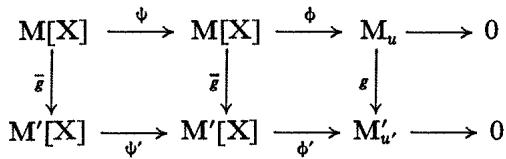
\includegraphics[keepaspectratio]{images/part004_f53e3a23.jpg}}

是交换的。

条件 \(g \circ u = u' \circ g\) 由 (43) 显然是使 \(g\) 成为 A{[}X{]}-同态的必要条件；它是充分的，因为它由归纳法蕴含 \(g \circ u^n = u'^n \circ g\) （对每个整数 \(n > 0\) ）。另一方面，对于所有 \(x \in M\) 以及所有 \(p \in A[X]\) ，

\[
\phi^ {\prime} (\bar {g} (p \otimes x)) = \phi^ {\prime} (p \otimes g (x)) = p (u ^ {\prime}) (g (x)) = g (p (u) (x)) = g (\phi (p \otimes x))
\]

和

\[
\bar {u} ^ {\prime} (\bar {g} (\boldsymbol {p} \otimes x)) = \bar {u} ^ {\prime} (\boldsymbol {p} \otimes g (x)) = \boldsymbol {p} \otimes u ^ {\prime} (g (x)) = \boldsymbol {p} \otimes g (u (x)) = \bar {g} (\bar {u} (\boldsymbol {p} \otimes x))
\]

这证明了图表(48)的交换性。

\subsection{自同态的特征多项式}

设 M 是维数为 n 的自由 A-模，u 是 M 的一个自同态。考虑两个不定元的多项式环 A{[}X, Y{]} 以及 A{[}X, Y{]}-模 M{[}X, Y{]} = A{[}X, Y{]} ⊗\_A M；令 \(\bar{u}\) 为由 u 典范地导出的 A{[}X, Y{]}-模 M{[}X, Y{]} 的自同态（II，§5，第1号）。由第 5 号命题 11 可知，

\[
\det (\mathbf {X} - \mathbf {Y} \bar {\boldsymbol {u}}) = \sum_ {j = 0} ^ {n} (- 1) ^ {j} \operatorname{Tr} \left(\bigwedge^ {j} (u)\right) \mathbf {X} ^ {n - j} \mathbf {Y} ^ {j}\tag{49}
\]

这是因为，若 \(U\) 是 \(u\) 关于某个基 \((e_i)_{1 \leqslant i \leqslant n}\) （ \(\mathbf{M}\) 的）的矩阵，则 \(U\) 就是 \(\bar{u}\) 关于基 \((1 \otimes e_i)_{1 \leqslant i \leqslant n}\) （ \(\mathbf{M}[\mathbf{X}, \mathbf{Y}]\) 的）的矩阵，因此

\[
\operatorname{Tr} \left(\bigwedge^ {j} (\bar {u})\right) = \operatorname{Tr} \left(\bigwedge^ {j} (u)\right).
\]

定义 3. 设 M 为有限维自由 A-模，u 为 M 的一个自同态。自同态 X - \(\bar{u}\) （自由 A{[}X{]}-模 M{[}X{]} 的）的行列式称为 u 的特征多项式，记作 \(\chi_u(X)\) 。

若 \(\mathbf{M}\) 的秩为 \(n\) ，则由 (49) 可知

\[
\chi_ {u} (\mathbf {X}) = \sum_ {j = 0} ^ {n} (- 1) ^ {j} \operatorname{Tr} \left(\bigwedge^ {j} (u)\right) \mathbf {X} ^ {n - j}\tag{50}
\]

因为 \(\operatorname{det}(\mathbf{X} - \mathbf{Y}\bar{u}) = \operatorname{det}(\mathbf{X}.I_n + \mathbf{Y}U)\) 且 \(\operatorname{det}(\mathbf{X} - \bar{u}) = \operatorname{det}(\mathbf{X}.I_n - U)\) 。由此可以看出 \(\chi_u(\mathbf{X})\) 是一个次数为 \(n\) 的首一多项式，其中 \(\mathbf{X}^{n-1}\) 的系数是 \(-\mathrm{Tr}(u)\) ，常数项是 \((-1)^n \operatorname{det}(u)\) 。

命题 20（”凯莱-哈密顿定理”）。对于有限维自由 A-模的每个自同态 \(u\) ，有 \(\chi_u(u) = 0\) 。

在命题 18（§ 3，第 10 号）的记号下，对于所有 \(x \in \mathbf{M}\) ， \(\chi_u(u)(x)\) 是在映射 \(\phi\) 下 \(\chi_u(\mathbf{X}) \otimes x\) 的像。但若 \(v\) 是 \(\mathbf{M}[\mathbf{X}]\) 的自同态、即 \(\mathbf{X} - \bar{u}\) 的余转置（第 6 号），那么

\[
\chi_ {u} (\mathbf {X}) \otimes x = \chi_ {u} (\mathbf {X}) (1 \otimes x) = (\mathbf {X} - \bar {u}) (v (1 \otimes x))
\]

且结论由第 10 号的命题 18 得出。

\section{范数与迹}

在本段中，K 表示一个交换环，A 是一个带单位的结合 K-代数。每个 A-模均假定具有通过将标量限制到 K 而得到的 K-模结构。
% semantic-fragments: legacy-input-seam
\relax{}
\subsection{相对于模的范数与迹}

定义1. 设 M 是一个 A-模，且作为 K-模具有有限基。对所有 \(a \in \mathbf{A}\) ，设 \(a_{\mathbf{M}}\) 为 K-模 M 的自同态 \(x \mapsto ax\) 。 \(a_{\mathbf{M}}\) 的迹、行列式和特征多项式分别称为 \(z\) 相对于 M 的迹、范数和特征多项式。

因此，a 的迹和范数是 K 的元素，分别记为 \(\mathrm{Tr}_{\mathbf{M}/\mathbf{K}}(a)\) 和 \(\mathrm{N}_{\mathbf{M}/\mathbf{K}}(a)\) ；a 的特征多项式是 K{[}X{]} 的元素，记作 \(\mathrm{Pc}_{\mathbf{M}/\mathbf{K}}(a;\mathbf{X})\) 。当没有混淆风险时，我们在上述记号中省略 K。

由自同态的迹和行列式的性质（II，第4节，第3小节及第8节，第1小节），我们得到关系式

\[
\operatorname{Tr} _ {\mathbf {M}} (a + a ^ {\prime}) = \operatorname{Tr} _ {\mathbf {M}} (a) + \operatorname{Tr} _ {\mathbf {M}} (a ^ {\prime})\tag{1}
\]

\begin{enumerate}
\def\labelenumi{(\arabic{enumi})}
\setcounter{enumi}{1}
\tightlist
\item
\end{enumerate}

\[
\operatorname{Tr} _ {\mathbf {M}} (a a ^ {\prime}) = \operatorname{Tr} _ {\mathbf {M}} (a ^ {\prime} a)\tag{3}
\]

\[
\mathrm{N} _ {\mathbf {M}} (a a ^ {\prime}) = \mathrm{N} _ {\mathbf {M}} (a) \mathrm{N} _ {\mathbf {M}} (a ^ {\prime})
\]

对 A 中所有 \(a, a'\) 成立。

设 \((e_i)_{1\leq i\leq n}\) 是 K-模 M 的一组基，且 \((m_{ij}(a))\) 是自同态 \(a_{\mathbf{M}}\) 关于这组基的矩阵。函数 \(m_{ij}\) 是K-模A上的线性形式，且

\begin{enumerate}
\def\labelenumi{(\arabic{enumi})}
\setcounter{enumi}{3}
\tightlist
\item
\end{enumerate}

\[
\operatorname{Tr} _ {\mathbf {M}} (a) = \sum_ {i = 1} ^ {n} m _ {i i} (a)\tag{5}
\]

\[
\mathrm{N} _ {\mathbf {M}} (a) = \det (m _ {i j} (a))\tag{6}
\]

\[
\operatorname{Pc} (a; \mathbf {X}) = \det (\delta_ {i j} \mathbf {X} - m _ {i j} (a)).
\]

由计算行列式的方法（第8节，第11小节，公式(50)）可知

\[
\mathrm{Pc} _ {\mathbf {M}} (a; \mathbf {X}) = \mathbf {X} ^ {n} + c _ {1} \mathbf {X} ^ {n - 1} + \dots + c _ {n}\tag{7}
\]

其中

\[
c _ {1} = - \operatorname{Tr} _ {\mathbf {M}} (a), \quad c _ {n} = (- 1) ^ {n} \mathrm{N} _ {\mathbf {M}} (a).\tag{8}
\]

对于 \(\lambda \in \mathbf{K}\) ，

\[
\operatorname{Tr} _ {\mathbf {M}} (\lambda) = n. \lambda , \quad \mathrm{N} _ {\mathbf {M}} (\lambda) = \lambda^ {n}, \quad \operatorname{Pc} _ {\mathbf {M}} (\lambda ; \mathbf {X}) = (\mathbf {X} - \lambda) ^ {n}.\tag{9}
\]

设 \(\mathbf{K}'\) 是一个交换 K-代数。设 \(\mathbf{M}' = \mathbf{K}' \otimes_{\mathbf{K}} \mathbf{M}\) 和 \(\mathbf{A}' = \mathbf{K}' \otimes_{\mathbf{K}} \mathbf{A}\) ，于是 \(\mathbf{M}'\) 具有一个 A'-模结构（§4，例 2）。作为 \(\mathbf{K}'\) -模， \(\mathbf{M}'\) 具有由 \(1 \otimes e_i\) ( \(1 \leqslant i \leqslant n\) ) 组成的基，且 \(a_{\mathbf{M}}\) 关于 \((e_i)\) 的矩阵等于 \((1 \otimes a)_{\mathbf{M}'}\) 关于 \((e_i')\) 的矩阵。则

\[
\operatorname{Tr} _ {\mathbf {M} ^ {\prime}} (1 \otimes a) = \operatorname{Tr} _ {\mathbf {M}} (a). 1, \quad \mathrm{N} _ {\mathbf {M} ^ {\prime}} (1 \otimes a) = \mathrm{N} _ {\mathbf {M}} (a). 1\tag{12}
\]

\[
\mathrm{Pc} _ {\mathbf {M} ^ {\prime}} (1 \otimes a; \mathbf {X}) = \mathrm{Pc} _ {\mathbf {M}} (a; \mathbf {X}). 1
\]

对所有 \(a \in \mathbf{A}\) 成立，其中 1 表示 \(\mathbf{K}'\) 的单位元。特别地，若我们取 \(\mathbf{K}' = \mathbf{K}[\mathbf{X}]\) ，则

\[
\mathrm{Pc} _ {\mathbf {M} / \mathbf {K}} (a; \mathbf {X}) = \mathrm{N} _ {\mathbf {M} [ \mathbf {X} ] / \mathbf {K} [ \mathbf {X} ]} (\mathbf {X} - a).\tag{13}
\]

\subsection{相对于模的范数与迹的性质}

若 \(\mathbf{M}\) 和 \(\mathbf{M}'\) 是两个同构的 A-模，且在 \(\mathbf{K}\) 上具有有限基，那么对所有 \(a \in \mathbf{A}\) ，

\[
\operatorname{Tr} _ {\mathbf {M} ^ {\prime}} (a) = \operatorname{Tr} _ {\mathbf {M}} (a), \quad \mathrm{N} _ {\mathbf {M} ^ {\prime}} (a) = \mathrm{N} _ {\mathbf {M}} (a), \quad \operatorname{Pc} _ {\mathbf {M} ^ {\prime}} (a; \mathbf {X}) = \operatorname{Pc} _ {\mathbf {M}} (a; \mathbf {X})\tag{14}
\]

因为若 \(f\) 是从 \(\mathbf{M}\) 到 \(\mathbf{M}'\) 的同构，则 \(a_{\mathbf{M}}\) 关于基 \(\mathbf{B}\) （ \(\mathbf{M}\) 在 \(\mathbf{K}\) 上的一个基）的矩阵，与 \(a_{\mathbf{M}'}\) 关于基 \(f(\mathbf{B})\) （ \(\mathbf{M}'\) 的基）的矩阵相同。

命题 1. 设 \(\mathbf{M} = \mathbf{M}_0 \supset \mathbf{M}_1 \supset \cdots \supset \mathbf{M}_r = \{0\}\) 是 A-模 \(\mathbf{M}\) 的子模的一个递减序列，使得每个 K-模 \(\mathbf{P}_i = \mathbf{M}_{i-1} / \mathbf{M}_i\) ( \(1 \leqslant i \leqslant r\) ) 都具有有限基。则 K-模 \(\mathbf{M}\) 具有有限基，并且

\[
\operatorname{Tr} _ {\mathbf {M}} (a) = \sum_ {i = 1} ^ {r} \operatorname{Tr} _ {\mathrm{P} _ {i}} (a), \quad \mathrm{N} _ {\mathbf {M}} (a) = \prod_ {i = 1} ^ {r} \mathrm{N} _ {\mathrm{P} _ {i}} (a)\tag{15}
\]

\[
\mathrm{Pc} _ {\mathbf {M}} (a; \mathbf {X}) = \prod_ {i = 1} ^ {r} \mathrm{Pc} _ {\mathbf {P} _ {i}} (a; \mathbf {X}).
\]

设 \(B_{i}^{\prime}\) 是 \(P_{i}\) 在 K 上的一组基；则 \(B_{i}\) 作为 \(B_{i}^{\prime}\) (模 \(M_{i}\) ) 的一个代表系，是 K-模 \(M_{i}\) 在 K-模 \(M_{i-1}\) 中的一个补子模的基（II，§1，第11号，命题21）。诸 \(B_{i}\) ( \(1 \leqslant i \leqslant r\) ) 的并集 B 是 M 在 K 上的一组基。设 \(X_{ii}\) 是自同态 \(a_{P_{i}}\) 关于基 \(B_{i}^{\prime}\) 的矩阵。立即可以看出， \(a_{M}\) 关于 B 的矩阵具有如下形式

\[
\left( \begin{array}{c c c c c} X _ {r r} & X _ {r, r - 1} & \ldots & X _ {r, 1} \\ 0 & X _ {r - 1, r - 1} & \ldots & X _ {r - 1, 1} \\ \cdot & \cdot & \cdot & \cdot & \cdot \\ 0 & 0 & \ldots & X _ {1 1} \end{array} \right)
\]

于是命题由第 1 号中的公式 (4)、(5)、(6) 以及 § 8 第 6 号中的公式 (31) 得出。

命题 2. 设 A、A' 为两个 K-代数，M 为 A-模，M' 为 A'-模。假设 M 与 M' 是维数分别为 n 与 n' 的自由 K-模，并将 M ⊗K M' 视为 (A ⊗K A')-模（§ 4，第 3 号，例 2）。那么，对于 a \ensuremath{\in} A 与 a' \ensuremath{\in} A'，

\begin{enumerate}
\def\labelenumi{(\arabic{enumi})}
\setcounter{enumi}{15}
\tightlist
\item
\end{enumerate}

\[
\operatorname{Tr} _ {\mathbf {M} \otimes \mathbf {M}} (a \otimes a ^ {\prime}) = \operatorname{Tr} _ {\mathbf {M}} (a) \operatorname{Tr} _ {\mathbf {M} ^ {\prime}} (a ^ {\prime})\tag{17}
\]

\[
\mathrm{N} _ {\mathbf {M} \otimes \mathbf {M} ^ {\prime}} (a \otimes a ^ {\prime}) = (\mathrm{N} _ {\mathbf {M}} (a)) ^ {n ^ {\prime}} (\mathrm{N} _ {\mathbf {M} ^ {\prime}} (a ^ {\prime})) ^ {n}.
\]

公式(16)由II，§4，第4号，公式(26)得出，而公式(17)由§8，第6号，公式(33)得出。

\subsection{代数中的范数与迹}

定义2. 设 A 是一个 K-代数，且它是有限维自由 K-模。对每个元素 \(a \in \mathbf{A}\) ，a 相对于 A 和 K 的迹（相应地，范数†，相应地，特征多项式）是 K-模 A 的自同态 \(x \mapsto ax\) 的迹（相应地，行列式，相应地，特征多项式）。

 \(a \in A\) 相对于 A 和 K 的迹、范数和特征多项式分别记为 \(\operatorname{Tr}_{\mathbf{A}/\mathbf{K}}(a)\) ， \(\operatorname{N}_{\mathbf{A}/\mathbf{K}}(a)\) 和 \(\operatorname{Pc}_{\mathbf{A}/\mathbf{K}}(a; \mathbf{X})\) ；当没有混淆风险时，我们在此记号中省略 K 甚至 A。注意， \(a \in A\) 的迹（相应地，范数、特征多项式）就是 a 相对于 A-模 \(A_{s}\) 的迹（相应地，范数，特征多项式）。

假设 A 是乘积 \(A_{1} \times A_{2} \times \cdots \times A_{m}\) ，即有限个 K 上的有限维代数（它们均为自由 K-模）的乘积。利用上述注记以及第 2 号的命题 1，对每个元素

\[
a = (a _ {1}, \dots , a _ {m}) \in \mathrm{A},
\]

\[
\mathrm{Tr} _ {\mathbf {A} / \mathbb {K}} (a) = \sum_ {i = 1} ^ {m} \mathrm{Tr} _ {\mathbf {A} _ {i} / \mathbb {K}} (a _ {i}), \qquad \mathrm{N} _ {\mathbf {A} / \mathbb {K}} (a) = \prod_ {i = 1} ^ {m} \mathrm{N} _ {\mathbf {A} _ {i} / \mathbb {K}} (a _ {i})\tag{18}
\]

\[
\mathrm{Pc} _ {\mathbf {A} / \mathbf {K}} (a; \mathbf {X}) = \prod_ {i = 1} ^ {m} \mathrm{Pc} _ {\mathbf {A} _ {i} / \mathbf {K}} (a _ {i}; \mathbf {X}).
\]

类似地，第 2 号的命题 2 表明，若 A 和 A' 是两个代数，它们都是自由 K-模，在 K 上的维数分别为 n 与 \(n'\) ，则对于 \(a \in A\) ， \(a' \in A'\) 。

\begin{enumerate}
\def\labelenumi{(\arabic{enumi})}
\setcounter{enumi}{18}
\tightlist
\item
\end{enumerate}

\[
\operatorname{Tr} _ {\mathbf {A} \otimes \mathbf {A} ^ {\prime}} (a \otimes a ^ {\prime}) = \operatorname{Tr} _ {\mathbf {A}} (a) \operatorname{Tr} _ {\mathbf {A} ^ {\prime}} (a ^ {\prime})\tag{20}
\]

\[
\mathrm{N} _ {\mathbf {A} \otimes \mathbf {A} ^ {\prime}} (a \otimes a ^ {\prime}) = (\mathrm{N} _ {\mathbf {A}} (a)) ^ {n ^ {\prime}} (\mathrm{N} _ {\mathbf {A} ^ {\prime}} (a ^ {\prime})) ^ {n}.
\]

最后，设 A 为 K 上的有限维代数，且它是自由 K-模，h 为 K 到交换环 \(K'\) 的一个同态， \(A' = A_{(K')}\) 为通过 h 作标量扩张而由 A 得到的 \(K'\) -代数。由第 1 号公式 (12) 可知，对所有 \(a \in A\) ，

\[
\begin{array}{r l} \mathrm{Tr} _ {\mathbf {A} ^ {\prime} / \mathbf {K} ^ {\prime}} (1 \otimes a) & = h (\mathrm{Tr} _ {\mathbf {A} / \mathbf {K}} (a)), \quad \mathrm{N} _ {\mathbf {A} ^ {\prime} / \mathbf {K} ^ {\prime}} (1 \otimes a) = h (\mathrm{N} _ {\mathbf {A} / \mathbf {K}} (a)) \\ \mathrm{Pc} _ {\mathbf {A} ^ {\prime} / \mathbf {K} ^ {\prime}} (1 \otimes a; \mathbf {X}) & = \tilde {h} (\mathrm{Pc} _ {\mathbf {A} / \mathbf {K}} (a; \mathbf {X})) \end{array}\tag{21}
\]

其中 \(\tilde{h}\) 是同态 \(\mathbf{K}[\mathbf{X}] \to \mathbf{K}'[\mathbf{X}]\) ，它由 \(h\) 导出。特别地，对于 \(\mathbf{K}' = \mathbf{K}[\mathbf{X}]\) ，记 \(\mathrm{A}[\mathbf{X}] = \mathrm{A} \otimes_{\mathbf{K}} \mathbf{K}[\mathbf{X}]\) ，我们得到

\[
\mathrm{Pc} _ {\mathbf {A} / \mathbf {K}} (a; \mathbf {X}) = \mathrm{N} _ {\mathbf {A} [ \mathbf {X} ] / \mathbf {K} [ \mathbf {X} ]} (\mathbf {X} - a).\tag{22}
\]

更一般地，若 \(\mathbf{K}'\) 是交换 \(\mathbf{K}\) -代数且 \(\mathbf{A}' = \mathbf{A} \otimes_{\mathbf{K}} \mathbf{K}'\) ，则对所有 \(x \in \mathbf{A}'\) ，

\[
\mathrm{Pc} _ {\mathbf {A} / \mathbf {K}} (a; x) = \mathrm{N} _ {\mathbf {A} ^ {\prime} / \mathbf {K} ^ {\prime}} (x - a).
\]

例子。(1) 设 A 是 K 上类型为 \((\alpha, \beta)\) 的二次代数， \((e_1, e_2)\) 是一个类型为 \((\alpha, \beta)\) 的基（§ 2，第 3 号）。对于 \(x = \xi e_1 + \eta e_2\) ， \(\operatorname{Tr}_{A/K}(x) = 2\xi + \beta \eta\) 和 \(\mathrm{N}_{A/K}(x) = \xi^2 + \beta \xi \eta - \alpha \eta^2\) ；因此这些函数与 \(x\) 的凯莱迹和凯莱范数相同（§ 2，第 24 号）。

\begin{enumerate}
\def\labelenumi{(\arabic{enumi})}
\setcounter{enumi}{1}
\item
  设 A 是 K 上的一个四元数代数。直接计算可以验证 \(\mathrm{Tr}_{\mathbf{A} / \mathbb{K}}(x) = 2\mathrm{T}(x)\) 和 \(\mathrm{N}_{\mathbf{A} / \mathbb{K}}(x) = (\mathrm{N}(x))^2\) ，其中 \(\mathbf{T}\) 和 \(\mathbf{N}\) 是凯莱迹和凯莱范数（§ 2，第 4 号）。
\item
  设 \(\mathbf{A} = \mathbf{M}_n(\mathbf{K})\) ，并令 \((E_{ij})\) （ \(\mathbf{A}\) 的典范基，II，§ 10，第 3 号）按字典序排列。则立即可见，对每个矩阵 \(\mathbf{X} = \sum_{i,j} \xi_{ij} E_{ij}\) ，（ \(n^2\) 阶的）自同态 \(Y \mapsto XY\) 的矩阵具有形式
\end{enumerate}

\[
\left( \begin{array}{c c c c} X & 0 & \ldots & 0 \\ 0 & X & \ldots & 0 \\ . & . & . & . \\ 0 & 0 & \ldots & X \end{array} \right)
\]

，因此 \(\operatorname{Tr}_{\mathbf{A} / \mathbb{K}}(X) = n.\operatorname{Tr}(X)\) 和 \(\mathrm{N}_{\mathbf{A} / \mathbb{K}}(X) = (\det (X))^n\)

\subsection{代数中范数与迹的性质}

命题3. 设 A 是一个具有有限基的 K-代数。元素 \(a \in \mathbf{A}\) 可逆的必要且充分条件是它的 \(\mathbf{N}_{\mathbf{A} / \mathbf{K}}(a)\) 在 \(\mathbf{K}\) 中可逆。

若 \(a\) 具有逆元 \(a'\) （位于 \(\mathbf{A}\) 中），则

\[
\mathrm{N} _ {\mathbf {A} / \mathbf {K}} (a) \mathrm{N} _ {\mathbf {A} / \mathbf {K}} (a ^ {\prime}) = \mathrm{N} _ {\mathbf {A} / \mathbf {K}} (a a ^ {\prime}) = \mathrm{N} _ {\mathbf {A} / \mathbf {K}} (1) = 1
\]

由第 1 号公式 (3)。反之，若 \(\mathbf{N}_{\mathbf{A} / \mathbb{K}}(a)\) 可逆，则自同态 \(h: x \mapsto ax\) 是双射（§ 8，第 2 号，定理 1）。于是存在 \(a' \in A\) 使得 \(aa' = 1\) ；于是 \(h(a'a - 1) = aa'a - a = (aa' - 1)a = 0\) ，从而 \(aa' = 1\) ，因为 \(h\) 是单射。因此 \(a'\) 是 \(a\) 的逆元。

命题4. 设 A 是一个具有有限基的 K-代数。对所有 \(a \in \mathbf{A}\) ， \(\operatorname{Pc}_{\mathbf{A} / \mathbf{K}}(a; a) = 0\) 。

这直接由凯莱-哈密顿定理（§ 8，第 11 号，命题 20）得出。

命题5. 设 A 是一个 K-代数，m 是 A 的一个双边理想。假设 \(A_{0} = A/m\) 是维数为 n 的自由 K-模，存在整数 r \textgreater{} 0 使得 \(m^{r} = \{0\}\) ，并且 \(m^{i-1}/m^{i}\) 是自由 \(A_{0}\) -模，其维数为 \(s_{i}\) （ \(1 \leqslant i \leqslant r\) ）。设 \(s = s_{1} + \cdots + s_{r}\) ，且对所有 \(a \in A\) ，设 \(a_{0}\) 表示 a 模 m 所在的类。则 A 是维数为 ns 的自由 K-模，且对所有 \(a \in A\) ，

\[
\operatorname{Tr} _ {\mathbf {A}} (a) = s. \operatorname{Tr} _ {\mathbf {A} _ {0}} (a _ {0}), \quad \mathrm{N} _ {\mathbf {A}} (a) = (\mathrm{N} _ {\mathbf {A} _ {0}} (a _ {0})) ^ {s}\tag{23}
\]

\[
\mathrm{Pc} _ {\mathbf {A}} (a; \mathbf {X}) = (\mathrm{Pc} _ {\mathbf {A} _ {0}} (a _ {0}; \mathbf {X})) ^ {s}.
\]

根据 II，§1，第 13 号，命题 25， \(\mathfrak{m}^{i - 1} / \mathfrak{m}^{i}\) 是维数为 \(ns_i\) 的自由 K-模。因此，第 2 号中的命题 1 可以应用于 \(\mathbf{P}_i = \mathfrak{m}^{i - 1} / \mathfrak{m}^{i}\) ；

这首先表明 A 是一个维数为 \(n(s_{1} + \cdots + s_{r}) = ns\) 的自由 K-模。此外，该假设蕴含 A-模 \(P_{i}\) 同构于 \(s_{i}\) 个子模的直和，这些子模均同构于 A-模 \(A_{0}\) ；由第 2 号命题 1，因此 \(\mathrm{N}_{\mathrm{P}_{i}}(a) = \mathrm{N}_{\mathrm{A}_{0}}(a)^{s_{i}}\) ；最终因此

\[
\mathrm{N} _ {\mathbf {A}} (a) = \mathrm{N} _ {\mathbf {A} _ {0}} (a) ^ {s}.
\]

在此公式中， \(\mathrm{N}_{\mathbf{A}_{0}}(a)\) 是通过将 \(A_{0}\) 视为左 A-模来定义的，它等于 K-线性映射 \(x \mapsto ax\) 在 \(A_{0}\) 到自身上的行列式；但由于 \(ax = a_{0}x\) 对 \(x \in A_{0}\) 成立，故 \(\mathrm{N}_{\mathbf{A}_{0}}(a) = \mathrm{N}_{\mathbf{A}_{0}}(a_{0})\) ，这就完成了范数公式 (23) 的证明。另外两个公式可类似地证明。

命题6. 设 A 是 K 上的一个交换代数，且在 K 上具有有限基，V 是一个 A-模，且在 A 上具有有限基。则 V 在 K 上具有有限基，并且对 V 的每个 A-自同态 u，若 \(u_{\mathbf{K}}\) 是将u视为V的K自同态的映射，

\[
\operatorname{Tr} (u _ {\mathbb {K}}) = \operatorname{Tr} _ {\mathbf {A} / \mathbb {K}} (\operatorname{Tr} (u)), \quad \det (u _ {\mathbb {K}}) = \mathrm{N} _ {\mathbf {A} / \mathbb {K}} (\det (u))\tag{24}
\]

\[
\operatorname{Pc} (u _ {\mathbf {K}}; \mathbf {X}) = \mathrm{N} _ {\mathbf {A} [ \mathbf {X} ] / \mathbf {K} [ \mathbf {X} ]} (\operatorname{Pc} (u; \mathbf {X})).
\]

设 \((a_{i})_{1\leqslant i\leqslant m}\) 是 A 在 K 上的一个基， \((e_{j})_{1\leqslant j\leqslant n}\) 是 V 在 A 上的一个基；则 \((a_{i}e_{j})\) 是 V 在 K 上的一个基（II，§1，第13号，命题25）。另一方面，将第二个公式应用于自同态 \(\mathbf{X} - \bar{\boldsymbol{u}}\) （即 A{[}X{]}-模 A{[}X{]} \(\otimes_{\mathbf{A}}\mathrm{V}\) 的自同态）（§ 8，第 10 号），即可导出公式 (24) 中的第三个。因此，只需证明 (24) 中的前两个公式即可。我们首先建立以下引理：

引理1. 设 \(\mathbf{X}_{ij}\) ( \(1 \leqslant i \leqslant n\) , \(1 \leqslant j \leqslant n\) ) 是 \(n^2\) 个未定元， \(X\) 是元素为 \((\mathbf{X}_{ij})\) 的 \(n\) 阶方阵， \(\mathbf{D}(\mathbf{X}_{11}, \ldots, \mathbf{X}_{nn}) \in \mathbf{Z}[\mathbf{X}_{11}, \ldots, \mathbf{X}_{nn}]\) 是行列式 \(\det(X)\) 。另一方面，设 A 为交换环， \(\mathbf{M}_{ij}\) ( \(1 \leqslant i \leqslant n\) , \(1 \leqslant j \leqslant n\) ) 是 A 上的 \(n^2\) 个 \(m\) 阶矩阵，它们两两可交换，M 是 A 上的 \(mn\) 阶方阵，它可以表示为矩阵的分块方阵（II，§10，第7号）

\[
M = \left( \begin{array}{c c c c} M _ {1 1} & M _ {1 2} & \ldots & M _ {1 n} \\ M _ {2 1} & M _ {2 2} & \ldots & M _ {2 n} \\ \cdot & \cdot & \cdot & \cdot \\ M _ {n 1} & M _ {n 2} & \ldots & M _ {n n} \end{array} \right)
\]

那么M的行列式等于方阵的行列式

\[
\mathrm{D} (M _ {1 1}, \dots , M _ {n n})
\]

该方阵的阶为 m。

我们对 \(n\) 进行归纳，情形 \(n = 0\) 和 \(n = 1\) 是平凡的。

设 \(Z\) 为一个新的未定元， \(N_{ij}\) 表示矩阵 \(M_{ij} + \delta_{ij}ZI_m\) ( \(\delta_{ij}\) 为克罗内克指标)。若 \(D^{ij}(X_{11},\ldots,X_{nn})\) 是 \(X_{ij}\) 在矩阵 \(X\) （§ 8，第 6 号）中的代数余子式，则

\[
\mathrm{X} _ {j l} \mathrm{D} ^ {k l} (\mathrm{X} _ {1 1}, \dots , \mathrm{X} _ {n n}) = \delta_ {j k} \mathrm{D} (\mathrm{X} _ {1 1}, \dots , \mathrm{X} _ {n n})\tag{25}
\]

（§ 8，第 6 号，公式 (28)）。我们记 \(N_{ij}' = \mathbf{D}^{ij}(N_{11}, \ldots, N_{nn})\) ，这是一个 \(m\) 阶方阵，位于 \(\mathrm{A}[Z]\) 上；并考虑乘积 \(N.U\) ，其中

\[
U = \left( \begin{array}{c c c c} N _ {1 1} ^ {\prime} & 0 & \ldots & 0 \\ N _ {1 2} ^ {\prime} & I _ {m} & \ldots & 0 \\ \cdot & \cdot & \cdot & \cdot \\ N _ {1 n} ^ {\prime} & 0 & \ldots & I _ {m} \end{array} \right),
\]

\[
N = \left( \begin{array}{c c c c} N _ {1 1} & N _ {1 2} & \ldots & N _ {1 n} \\ N _ {2 1} & N _ {2 2} & \ldots & N _ {2 n} \\ \cdot & \cdot & \cdot & \cdot \\ N _ {n 1} & N _ {n 2} & \ldots & N _ {n n} \end{array} \right)
\]

按分块进行此乘积（II，§ 10，第 5 号）并利用公式 (25)，我们得到

\[
N. U = \left( \begin{array}{c c c c} P & N _ {1 2} & \ldots & N _ {1 n} \\ 0 & N _ {2 2} & \ldots & N _ {2 n} \\ \cdot & \cdot & \cdot & \cdot \\ 0 & N _ {n 2} & \ldots & N _ {n n} \end{array} \right)
\]

其中我们记作 \(P = \mathrm{D}(N_{11},\ldots ,N_{nn})\) 。设

\[
Q = \left( \begin{array}{c c c c} N _ {2 2} & \ldots & N _ {2 n} \\ \cdot & \cdot & \cdot & \cdot \\ N _ {n 2} & \ldots & N _ {n n} \end{array} \right)
\]

，这是一个 \(m(n - 1)\) 阶矩阵；则（§8，第6号，公式 (31)）(det \(N\) ) ( \(\det U\) ) = ( \(\det P\) ) ( \(\det Q\) ) 且 \(\det U = \det N_{11}'\) 。但根据归纳假设， \(\det Q = \det(\mathrm{D}^{11}(N_{11},\ldots ,N_{nn})) = \det N_{11}'\) ，并且根据 \(N_{ij}\) 的定义，显然 \(\det Q\) 是 A{[}Z{]} 中一个次数为 \(m(n - 1)\) 的多项式，其 \(Z^{m(n - 1)}\) 项的系数为 1；由此立即得出 \(\det Q\) 在分次代数 A{[}Z{]} 中不是零因子。因此我们得出结论： \(\det N = \det(\mathrm{D}(N_{11},\ldots ,N_{nn}))\) 在 A{[}Z{]} 中成立；如果我们在这些多项式中将 Z 替换为 0，那么 \(\det M = \det(\mathrm{D}(M_{11},\ldots ,M_{nn}))\) 。

证明了这一引理之后，K-模 V 是诸 K-模 \(Ae_{j}\) ( \(1 \leqslant j \leqslant n\) ) 的直和；我们记 \(u(e_{j}) = \sum_{k=1}^{n} c_{jk} e_{k}\) 。对每个元素 \(xe_{j} \in Ae_{j}\) ，其中 \(x \in A\) ， \(u(xe_{j})\) 在 \(Ae_{k}\) 中的分量是 \(xc_{jk} e_{k}\) ；由此可知， \(u_{k}\) 关于 K-模 V 的基 \((a_{i} e_{j})\) 的矩阵可以表示为分块方阵 \((M_{jk})\) 的形式，其中 \(M_{jk}\) 是 K-线性映射 \(xe_{j} \mapsto xc_{jk} e_{k}\) （它把 \(Ae_{j}\) 映到 \(Ae_{k}\) ）关于这两个 K-模的基 \((a_{i} e_{j})_{1 \leqslant i \leqslant m}\) 和 \((a_{i} e_{k})_{1 \leqslant i \leqslant m}\) （II，§ 10，第 5 号）的矩阵。若对所有 \(t \in A\) ， \(M(t)\) 表示 A 在 K 上的基 \((a_{i})_{1 \leqslant i \leqslant m}\) 下 A 的自同态 \(x \mapsto xt\) 的矩阵，则 \(M_{jk} = M(c_{jk})\) ；由于 \(t \mapsto M(t)\) 是一个环同态，矩阵 \(M_{jk}\) 两两可交换。则

\[
\det u _ {\mathrm{K}} = \det (\mathrm{D} (M _ {1 1}, \dots , M _ {n n}))
\]

由引理1。但由于 \(t \mapsto M(t)\) 是一个环同态， \(\mathrm{D}(M_{11},\ldots ,M_{nn})\) 是 A 的 K-自同态 \(x \mapsto x.\det (c_{jk})\) 关于基 \((a_t)\) 的矩阵；根据定义，其行列式因此为 \(\mathrm{N}_{\mathbf{A} / \mathbf{K}}(\det (u))\) ，这证明了 (24) 中的第二个公式。另一方面，

\[
\operatorname{Tr} \left(u _ {\mathrm{K}}\right) = \sum_ {j = 1} ^ {n} \operatorname{Tr} \left(M _ {j j}\right) = \sum_ {j = 1} ^ {n} \operatorname{Tr} _ {\mathrm{A} / \mathrm{K}} \left(c _ {j j}\right) = \operatorname{Tr} _ {\mathrm{A} / \mathrm{K}} \left(\sum_ {j = 1} ^ {n} c _ {j j}\right) = \operatorname{Tr} _ {\mathrm{A} / \mathrm{K}} (\operatorname{Tr} (u))
\]

并且命题6的证明完成。

推论。设A是交换K-代数，在K上具有有限基，B是A-代数，在A上具有有限基。则B在K上具有有限基，并且，对所有 \(b \in B\) （“传递性公式”）

\[
\operatorname{Tr} _ {\mathbf {B} / \mathbf {K}} (b) = \operatorname{Tr} _ {\mathbf {A} / \mathbf {K}} (\operatorname{Tr} _ {\mathbf {B} / \mathbf {A}} (b)), \quad \mathrm{N} _ {\mathbf {B} / \mathbf {K}} (b) = \mathrm{N} _ {\mathbf {A} / \mathbf {K}} (\mathrm{N} _ {\mathbf {B} / \mathbf {A}} (b))\tag{26}
\]

\[
\mathrm{Pc} _ {\mathbf {B} / \mathbf {K}} (b; \mathbf {X}) = \mathrm{N} _ {\mathbf {A} [ \mathbf {X} ] / \mathbf {K} [ \mathbf {X} ]} (\mathrm{Pc} _ {\mathbf {B} / \mathbf {A}} (b; \mathbf {X})).
\]

这直接从命题 6 得出，取 \(\mathbf{V} = \mathbf{B}\) 和 \(u(x) = bx\) 。

注记。假设 K 到 A 的同态 \(\lambda \mapsto \lambda, 1\) 是单射，并将 K 与其在 A 中的像等同；假设 A 作为 K-模具有有限基 \((e_i)_{1 \leqslant i \leqslant n}\) 。设 \(s\) 是 A 的一个自同构，使得 \(s(\mathbf{K}) = \mathbf{K}\) 。设 \(a\) 是 A 的一个元素；则通过转移结构

\begin{enumerate}
\def\labelenumi{(\arabic{enumi})}
\setcounter{enumi}{26}
\tightlist
\item
\end{enumerate}

\[
\operatorname{Tr} _ {\mathbf {A} / \mathbf {K}} (s (a)) = s (\operatorname{Tr} _ {\mathbf {A} / \mathbf {K}} (a))\tag{28}
\]

\[
\mathrm{N} _ {\mathbf {A} / \mathbf {K}} (s (a)) = s (\mathrm{N} _ {\mathbf {A} / \mathbf {K}} (a)).
\]

同时考虑 A 的一个导子 D（§ 10，第 2 号），使得 D(K) ⊂ K，并记 \(D (e _ {i}) = \sum_ {j = 1} ^ {n} e _ {j} \mu_ {j i}\) ，其中 \(\mu_ {j i} \in \mathbf {K}\) ；记

\[
a e _ {i} = \sum_ {j = 1} ^ {n} e _ {j} \lambda_ {j i} \quad \text { with } \quad \lambda_ {j i} \in \mathbf {K}.
\]

那么

\[
\mathrm{D} (a) e _ {i} + a \mathrm{D} (e _ {i}) = \mathrm{D} (a e _ {i}) = \sum_ {j = 1} ^ {n} (\mathrm{D} (e _ {j}) \lambda_ {j i} + e _ {j} \mathrm{D} (\lambda_ {j i})).
\]

由此可得

\[
\mathbf {D} (a) e _ {i} = \sum_ {j = 1} ^ {n} e _ {j} \nu_ {j i}
\]

其中 \(\nu_{ji} = \mathrm{D}(\lambda_{ji}) + \sum_{k=1}^{n} (\mu_{jk}\lambda_{ki} - \lambda_{jk}\mu_{ki})\) 。由于 \(\sum_{i,k} (\mu_{ik}\lambda_{ki} - \lambda_{ik}\mu_{ki}) = 0\) ，因此

 \(\mathrm{Tr}_{\mathbf{A} / \mathbb{K}}(\mathbf{D}(a)) = \sum_{i = 1}^{n}\mathbf{D}(\lambda_{ii})\) ，换言之

\[
\operatorname{Tr} _ {\mathbf {A} / \mathbf {K}} (\mathbf {D} (a)) = \mathbf {D} (\operatorname{Tr} _ {\mathbf {A} / \mathbf {K}} (a)). *\tag{29}
\]

\subsection{代数的判别式}

定义 3. 设 A 是一个 K-代数，具有由 n 个元素构成的有限基。A 中 n 个元素的序列 \((x_{1},\ldots,x_{n})\) 关于 K 的判别式，记作 \(\mathrm{D}_{\mathrm{A}/\mathrm{K}}(x_{1},\ldots,x_{n})\) ，定义为下述方阵的判别式

\[
\left(\operatorname{Tr} _ {\mathbf {A} / \mathbb {K}} \left(x _ {i} x _ {j}\right)\right) _ {1 \leqslant i \leqslant n, 1 \leqslant j \leqslant n}.
\]

首先考虑 A 在 K 上的一个基 \((e_i)_{1\leqslant i\leqslant n}\) ，并记

\[
e _ {i} e _ {j} = \sum_ {k = 1} ^ {n} c _ {i j k} e _ {k} \quad \text { with } \quad c _ {i j k} \in \mathbf {K}.\tag{30}
\]

那么 \(\mathrm{Tr}_{\mathbf{A} / \mathbf{K}}(e_i) = \sum_{s=1}^{n} c_{iss}\) ，由此 \(\mathrm{Tr}_{\mathbf{A} / \mathbf{K}}(e_i e_j) = \sum_{k,s} c_{ijk} c_{kss}\) ，进而

\[
\mathrm{D} _ {\mathrm{A} / \mathrm{K}} (e _ {1}, \dots , e _ {n}) = \det \left(\left(\sum_ {k, s} c _ {i j k} c _ {k s s}\right) _ {1 \leqslant i \leqslant n, 1 \leqslant j \leqslant n}\right).\tag{31}
\]

现在令 \((x_{i})_{1\leqslant i\leqslant n},(x_{i}^{\prime})_{1\leqslant i\leqslant n}\) 是 A 的 \(n\) 个元素的两个序列，并假设存在一个 \(n\) 阶方阵 \(M = (m_{ij})\) ，其系数在 K 中，使得 \(x_{i} = \sum_{j=1}^{n} m_{ij} x_{j}'\) 对 \(1 \leqslant i \leqslant n\) 成立。我们记

\[
T = \left(\operatorname{Tr} _ {\mathrm{A} / \mathrm{K}} \left(x _ {i} x _ {j}\right)\right) _ {1 \leqslant i \leqslant n, 1 \leqslant j \leqslant n}, \quad T ^ {\prime} = \left(\operatorname{Tr} _ {\mathrm{A} / \mathrm{K}} \left(x _ {i} ^ {\prime} x _ {j} ^ {\prime}\right)\right) _ {1 \leqslant i \leqslant n, 1 \leqslant j \leqslant n}.
\]

那么 \(\mathrm{Tr}_{\mathbf{A} / \mathbf{K}}(x_i x_j) = \sum_{p,q} m_{ip} m_{jq} \mathrm{Tr}_{\mathbf{A} / \mathbf{K}}(x_p' x_q')\) ，因此 \(T = M. T'.^t M\) ；于是行列式的乘法规则给出

\[
\det T = \det M. \det T ^ {\prime}. \det ^ {t} M = (\det M) ^ {2} \det T ^ {\prime}
\]

最终得到

\[
\mathrm{D} _ {\mathrm{A} / \mathrm{K}} (x _ {1}, \dots , x _ {n}) = (\det M) ^ {2} \mathrm{D} _ {\mathrm{A} / \mathrm{K}} (x _ {i} ^ {\prime}, \dots , x _ {n} ^ {\prime}).\tag{32}
\]

上述公式特别表明，A 在 K 上的两组基的判别式相差 K 中一个可逆元素的平方，因此生成 K 的同一个（主）理想。这个理想 \(\Delta_{A/K}\) 称为 A 在 K 上的判别式理想；由公式 (32)，A 中仅项的顺序不同的任意 n 个元素的序列都具有相同的判别式，因为置换矩阵的行列式等于 \(\pm1\) 。

例子。(1) 若 A 是 K 上类型为 \((\alpha, \beta)\) 的二次代数，则（采用 § 2 第 3 号的记号） \(\operatorname{Tr}(e_1) = 2\) ， \(\operatorname{Tr}(e_2) = \beta\) ，

\[
\operatorname{Tr} (e _ {2} ^ {2}) = \alpha \operatorname{Tr} (e _ {1}) + \beta \operatorname{Tr} (e _ {2}) = 2 \alpha + \beta^ {2},
\]

由此 \(\mathbf{D}_{\mathbf{A} / \mathbb{K}}(e_1,e_2) = \beta^2 +4\alpha .\)

\begin{enumerate}
\def\labelenumi{(\arabic{enumi})}
\setcounter{enumi}{1}
\item
  设 \(\mathbf{A} = \mathbf{K}[\mathbf{X}] / \mathbf{K}[\mathbf{X}]\mathbf{P}\) ，其中 \(\mathrm{P}(\mathbf{X}) = \mathbf{X}^3 + p\mathbf{X} + q\) ，于是若 \(x\) 是 \(\mathbf{X}\) 在 \(\mathbf{A}, 1, x, x^2\) 中的像，则它们构成 \(\mathbf{A}\) 在 \(\mathbf{K}\) 上的一组基，且 \(x^3 = -px - q\) 。立即可以看出 \(\operatorname{Tr}(1) = 3\) ， \(\operatorname{Tr}(x) = 0\) ， \(\operatorname{Tr}(x^2) = -2p\) ；利用关系 \(x^3 = -px - q\) ， \(\operatorname{Tr}(x^3) = -3q\) ， \(\operatorname{Tr}(x^4) = 2p^2\) ，由此容易得到 \(\mathrm{D}_{\mathbf{A} / \mathbf{K}}(1, x, x^2) = -4p^3 - 27q^2\) 。
\item
  设 A 是 K 上类型为 \((\alpha, \beta, \gamma)\) 的四元数代数， \((1, i, j, k)\) 是 A 的一个类型为 \((\alpha, \beta, \gamma)\) 的基；利用 § 3 第 5 号公式 (30)，容易得出 \(\operatorname{Tr}(1) = 4\) ， \(\operatorname{Tr}(i) = 2\beta\) ， \(\operatorname{Tr}(j) = \operatorname{Tr}(k) = 0\) ，于是
\end{enumerate}

\[
\mathrm{D} _ {\mathrm{A/K}} (1, i, j, k) = - 16 \gamma^ {2} (\beta^ {2} + 4 \alpha) ^ {2}.
\]

\begin{enumerate}
\def\labelenumi{(\arabic{enumi})}
\setcounter{enumi}{3}
\tightlist
\item
  设 \(\mathbf{A} = \mathbf{M}_n(\mathbf{K})\) ，并考虑典范基 \((E_{ij})_{1\leqslant i\leqslant n,1\leqslant j\leqslant n}\) （ \(\mathbf{A}\) 在 \(\mathbf{K}\) 上的）(II, § 10, 第 3 号)。立即可见 \(\operatorname{Tr}_{\mathbf{A} / \mathbf{K}}(E_{ij}) = 0\) （若 \(j\neq i\) ），且 \(\operatorname{Tr}_{\mathbf{A} / \mathbf{K}}(E_{ii}) = n\) 对所有 \(i\) 成立；由此不难得出，矩阵 \((\operatorname{Tr}(E_{ij}E_{hk}))\) （ \(n^2\) 阶）具有 \(n.P\) 的形式，其中 \(P\) 是一个置换矩阵，从而 \(\mathrm{D}_{\mathbf{A} / \mathbf{K}}((E_{ij})) = \pm n^{n^2}\) 。
\end{enumerate}

\section{导子}

在本节中，除非另有说明，所考虑的代数不假定为结合的，也不一定具有单位元；K 表示一个交换环。

\subsection{交换因子}

在本段中，当我们不加说明地提及分次时，总是指类型为 \(\Delta\) 的分次，其中 \(\Delta\) 是一个以加法记写的交换群。在本段中， \(\Delta\) 上取值于 Z 的交换因子称为 \(\Delta\) 上的交换因子（ \(\S\) 4，第 7 号，定义 6）。因此， \(\Delta\) 上的一个交换因子等同于一个映射 \(\varepsilon\colon(\alpha,\beta)\mapsto\varepsilon_{\alpha\beta}=\varepsilon(\alpha,\beta)\) ，它把 \(\Delta\times\Delta\) 映到乘法群 \(\{-1,1\}\) 中，使得对 \(\alpha,\alpha^{\prime},\beta,\beta^{\prime}\) （均为 \(\Delta\) 中的元素），

\[
\left\{ \begin{array}{l} \varepsilon (\alpha + \alpha^ {\prime}, \beta) = \varepsilon (\alpha , \beta) \varepsilon (\alpha^ {\prime}, \beta) \\ \varepsilon (\alpha , \beta + \beta^ {\prime}) = \varepsilon (\alpha , \beta) \varepsilon (\alpha , \beta^ {\prime}) \\ \varepsilon (\beta , \alpha) = \varepsilon (\alpha , \beta). \end{array} \right.\tag{1}
\]

由此可得 \(\varepsilon(2\alpha, \beta) = \varepsilon(\alpha, 2\beta) = 1\) .

当 \(\Delta = \mathbf{Z}\) 时，每个交换因子 \(\varepsilon\) 由 \(\varepsilon(1, 1)\) 的值决定；因此这样的因子只有两个，第一个由

\[
\varepsilon (p, q) = 1 \quad \text { for } \quad p, q \text { in } \mathbf {Z}\tag{2}
\]

定义，第二个由

\[
\varepsilon (p, q) = (- 1) ^ {p q} \quad \text { for } \quad p, q \text { in } \mathbf {Z}.\tag{3}
\]

\subsection{导子的一般定义}

考虑一个交换环 K，六个类型为 \(\Delta\) 的分次 K-模：A, A', A'', B, B', B''，以及三个 K-线性映射

\[
\mu \colon \mathrm{A} \times \mathrm{A} ^ {\prime} \rightarrow \mathrm{A} ^ {\prime \prime}, \quad \lambda_ {1} \colon \mathrm{B} \times \mathrm{A} ^ {\prime} \rightarrow \mathrm{B} ^ {\prime \prime}, \quad \lambda_ {2} \colon \mathrm{A} \times \mathrm{B} ^ {\prime} \rightarrow \mathrm{B} ^ {\prime \prime}
\]

使得相应的 K-线性映射

\[
\mathrm{A} \otimes_ {\mathrm{K}} \mathrm{A} ^ {\prime} \rightarrow \mathrm{A} ^ {\prime \prime}, \quad \mathrm{B} \otimes_ {\mathrm{K}} \mathrm{A} ^ {\prime} \rightarrow \mathrm{B} ^ {\prime \prime}, \quad \mathrm{A} \otimes_ {\mathrm{K}} \mathrm{B} ^ {\prime} \rightarrow \mathrm{B} ^ {\prime \prime}
\]

是次数为 0 的分次映射。像 \(\mu(a, a')\) （对于 \(a \in A\) ， \(a' \in A'\) ）简记为 \(a, a'\) 甚至 \(aa'\) ，另外两个双线性映射同理。因此 \(a, a'\) 的次数是 \(a\) 与 \(a'\) 的次数之和。

定义 1. 在上述设定和一个交换因子 \(\varepsilon\) （ \(\Delta \times \Delta\) 上的）之下，一个 \(\varepsilon\) -导子（或 \((\mathbf{K}, \varepsilon)\) -导子）（次数为 \(\delta \in \Delta\) ，从 \((\mathbf{A}, \mathbf{A}', \mathbf{A}'')\) 到 \((\mathbf{B}, \mathbf{B}', \mathbf{B}'')\) ）指的是次数为 \(\delta\) 的分次 K-线性映射的一个三元组：

\[
d \colon \mathrm{A} \rightarrow \mathrm{B}, \quad d ^ {\prime} \colon \mathrm{A} ^ {\prime} \rightarrow \mathrm{B} ^ {\prime}, \quad d ^ {\prime \prime} \colon \mathrm{A} ^ {\prime \prime} \rightarrow \mathrm{B} ^ {\prime \prime}
\]

的分次K-线性映射三元组，使得对每个齐次元素 \(a \in A\) 以及每个元素 \(a' \in A'\)

\[
d ^ {\prime \prime} (a. a ^ {\prime}) = (d a). a ^ {\prime} + \varepsilon_ {\delta , \deg (a)} a. (d ^ {\prime} a ^ {\prime}).\tag{4}
\]

显然，由线性性，只需在 \(a\) 和 \(a'\) 分别遍历 A 和 A' 的生成系时验证关系 (4) 即可。

把这三个映射 \(d, d', d''\) 用同一个字母 \(d\) 来表示往往是方便的（其合理性在于同样用 \(d\) 表示次数为 \(\delta\) 的分次 K-线性映射

\[
(a, a ^ {\prime}, a ^ {\prime \prime}) \mapsto (d a, d ^ {\prime} a ^ {\prime}, d ^ {\prime \prime} a ^ {\prime \prime})
\]

它把 \(\mathbf{A} \oplus \mathbf{A}' \oplus \mathbf{A}''\) 映到 \(\mathbf{B} \oplus \mathbf{B}' \oplus \mathbf{B}''\) 中。于是关系 (4) 可以更简单地写成

\[
d (a. a ^ {\prime}) = (d a). a ^ {\prime} + \varepsilon_ {\delta . \deg (a)} a. (d a ^ {\prime}).\tag{5}
\]

从 (A, A', A'') 到 (B, B', B'') 的给定次数的 \(\varepsilon\) -导子构成分次线性映射 K-模的一个子 K-模

\[
\operatorname{Homgr} _ {\mathbb {K}} (\mathrm{A} \oplus \mathrm{A} ^ {\prime} \oplus \mathrm{A} ^ {\prime \prime}, \mathrm{B} \oplus \mathrm{B} ^ {\prime} \oplus \mathrm{B} ^ {\prime \prime}).
\]

当 \(\varepsilon(\alpha, \beta) = 1\) 对所有 \(\alpha, \beta\) （ \(\Delta\) 中的）成立时，我们简称导子（或 K-导子）而不称 \(\varepsilon\) -导子。导子构成下列 K-模的一个子 K-模

\[
\operatorname{Hom} _ {\mathbb {K}} (\mathrm{A} \oplus \mathrm{A} ^ {\prime} \oplus \mathrm{A} ^ {\prime \prime}, \mathrm{B} \oplus \mathrm{B} ^ {\prime} \oplus \mathrm{B} ^ {\prime \prime}).
\]

当 \(\Delta = Z\) 且 \(\varepsilon(p, q) = (-1)^{pq}\) 时，每个偶次数的 \(\varepsilon\) -导子都是导子；每个奇次数的 \(\varepsilon\) -导子通常称为反导子（或 K-反导子）；于是反导子 d 满足

\[
d (a. a ^ {\prime}) = (d a). a ^ {\prime} + (- 1) ^ {\deg (a)} a. (d a ^ {\prime})\tag{6}
\]

对齐次元素 \(a \in A\) 成立。

注记。(1) 导子的概念可以推广到非分次模上，只需约定赋予这些模平凡分次结构即可。

\begin{enumerate}
\def\labelenumi{(\arabic{enumi})}
\setcounter{enumi}{1}
\tightlist
\item
  如果只考虑 \(\varepsilon\) -导子中次数为给定值 \(\delta\) 的那些，交换因子 \(\varepsilon\) 可以按如下方式消去：把双线性映射 \(\lambda_2: \mathbf{A} \times \mathbf{B}' \to \mathbf{B}''\) 替换为双线性映射 \(\lambda_2': \mathbf{A} \times \mathbf{B}' \to \mathbf{B}''\) ，使得对每个齐次元素 \(a\) （ \(\mathbf{A}\) 中的）以及所有 \(b' \in \mathbf{B}'\) ，
\end{enumerate}

\[
\lambda_ {2} ^ {\prime} (a, b ^ {\prime}) = \varepsilon_ {\delta , \deg (a)} \lambda_ {2} (a, b ^ {\prime}).
\]

那么 \(d\) 是关于双线性映射 \(\mu, \lambda_{1}, \lambda_{2}^{\prime}\) 的导子。

上述给出的 \(\varepsilon\) -导子的一般定义特别用于两种情况：

情形（I）：A = B， \(A' = B'\) , \(A'' = B''\) 且三个双线性映射 \(\mu\) , \(\lambda_{1}\) , \(\lambda_{2}\) 等于同一个映射。

情形（II）： \(\mathbf{A} = \mathbf{A}' = \mathbf{A}''\) ， \(\mathbf{B} = \mathbf{B}' = \mathbf{B}''\) ，因此（对于 \(\mu\) ） \(\mathbf{A}\) 是一个分次代数，且这两个 K-双线性映射

\[
\lambda_ {1} \colon \mathrm{B} \times \mathrm{A} \rightarrow \mathrm{B}, \quad \lambda_ {2} \colon \mathrm{A} \times \mathrm{B} \rightarrow \mathrm{B}\tag{7}
\]

使得相应的 K-线性映射 \(B \otimes_{K} A \to B\) ， \(A \otimes_{K} B \to B\) 是次数为 0 的分次映射。此时，一个 \(\varepsilon\) -导子（次数为 \(\delta\) ，从 A 到 B）是指一个分次 K-线性映射 \(d: A \to B\) （次数为 \(\delta\) ），使得对 A 中每个齐次元素 x 以及每个 \(y \in A\) ，我们有关系式

\[
d (x y) = (d x) y + \varepsilon_ {\delta , \deg (a)} x (d y).\tag{8}
\]

特别地，在情形 (II) 中考虑这样的情形：A 是带单位元的结合 K-代数，且 \(\lambda_{1}\) 和 \(\lambda_{2}\) 是一个 (A, A)-双模（§ 4，第 3 号，定义 3）的外部法则。特别当 A 和 B 是两个带单位元的结合 K-代数、给定分次 K-代数的一个带单位元的同态 \(\rho: A \to B\) 并在 B 上考虑由这两个外部法则定义的 (A, A)-双模结构时，上述情形成立

\[
\lambda_ {1} \colon (b, a) \mapsto b \rho (a), \quad \lambda_ {2} \colon (a, b) \mapsto \rho (a) b
\]

对于 \(a\in \mathbf{A},b\in \mathbf{B}.\)

情形（I）和（II）具有以下共同情形：考虑一个分次 K-代数 A，取 B = A，映射 (7) 均为 A 上的乘法。此时我们谈论分次代数 A 的 ε-导子（或 (K, ε)-导子）：它是 A 到自身的、次数为 δ 的分次 K-线性映射，对 A 中每个齐次元素 x 以及所有 \(y \in A\) 满足 (8)。特别地，若 A 是一个分次环（视为（结合的）Z-代数），我们就谈论环 A 的 ε-导子。

设A是一个含单位元的交换结合K-代数，B是一个A-模；当我们谈到从A到B的导子时，总是指B上由A-模结构导出的A-双模结构；此时公式

\[
d (x y) = x (d y) + y (d x) \quad \text { for } \quad x \in \mathrm{A}, y \in \mathrm{A}\tag{9}
\]

对这样的导子 \(d: A \rightarrow B\) 成立。

\subsection{导子的例子}

例 1. *设 A 是 R 到 R 的可微映射构成的 R-代数，并设 \(x_0\) 是 R 的一个点；R 可视为一个 A-模，其外运算为 \((f, a) \mapsto f(x_0)a\) 。则映射 \(f \mapsto \mathrm{D}f(x_0)\) 是一个导子，因为（实变函数，I，§ 1，第 3 号）

\[
(\mathbf {D} (f g)) (x _ {0}) = (\mathbf {D} f (x _ {0})) g (x _ {0}) + f (x _ {0}) (\mathbf {D} g (x _ {0})). *
\]

例 2. *设 X 是一个 C∞ 类可微流形，并设 A 为 X 上微分形式的分次 R-代数。将每个微分形式 ω 映到其外微分 dω 的映射是次数为 +1 的反导子（可微与解析流形，R，§ 8）。*

例 3. 设 A 是一个结合 K-代数。对所有 \(a \in \mathbf{A}\) ，映射 \(x \mapsto ax - xa\) 是代数 A 的一个导子（参见第 6 号）。

例 4. 设 M 是一个 K-模，A 是带通常分次的外代数 \(\bigwedge (\mathbf{M}^{*})\) （§ 7，第 1 号）。将在 § 11 第 9 号中看到，对所有 \(x\in \mathbf{M}\) ，右内积 \(i(x)\) 是 A 的一个次数为 \(-1\) 的反导子。*

例 5. 回到第 2 号定义 1 的一般情形，设 \(\overline{\mathbf{K}}\) 是另一个交换环，且 \(\rho: \mathbf{K} \to \overline{\mathbf{K}}\) 是一个环同态；设 \(\overline{\mathbf{A}}, \overline{\mathbf{A}'}\) ， \(\overline{\mathbf{A}''}\) ， \(\overline{\mathbf{B}}, \overline{\mathbf{B}'}\) ， \(\overline{\mathbf{B}''}\) 表示分次 \(\overline{\mathbf{K}}\) -模，它们分别由 \(\mathbf{A}, \mathbf{A}', \mathbf{A}''\) ， \(\mathbf{B}, \mathbf{B}'\) ， \(\mathbf{B}''\) 通过将标量环扩张到 \(\overline{\mathbf{K}}\) 而得到（II，§ 11，第 5 号）；我们由 \(\mu\) ， \(\lambda_1\) 和 \(\lambda_2\) 导出 \(\overline{\mathbf{K}}\) -双线性映射

\[
\bar {\mu}: \overline {{{A}}} \times \overline {{{A}}} ^ {\prime} \rightarrow \overline {{{A}}} ^ {\prime \prime}, \quad \bar {\lambda} _ {1}: \bar {B} \times \overline {{{A}}} ^ {\prime} \rightarrow \bar {B} ^ {\prime \prime}, \quad \bar {\lambda} _ {2}: \overline {{{A}}} \times \bar {B} ^ {\prime} \rightarrow \bar {B} ^ {\prime \prime}
\]

作 \(l_{\bar{K}}\) 与 \(\mu\) ， \(\lambda_{1}\) 和 \(\lambda_{2}\) 相应的 K-线性映射的张量积（II, § 5, 第 1 号）。那么，若 d 是一个 \(\varepsilon\) -导子（次数为 \(\delta\) ，从 \((\mathbf{A}, \mathbf{A}', \mathbf{A}^{\prime\prime})\) 到 \((\mathbf{B}, \mathbf{B}', \mathbf{B}^{\prime\prime})\) ），则映射 \(\bar{d} = d \otimes l_{\bar{K}}\) （从 \(\overline{A} \oplus \overline{A}' \oplus \overline{A}''\) 到 \(\overline{B} \oplus \overline{B}' \oplus \overline{B}''\) ）是一个 \(\varepsilon\) -导子（次数为 \(\delta\) ，从 \((\overline{A}, \overline{A}', \overline{A}^{\prime\prime})\) 到 \((\overline{B}, \overline{B}', \overline{B}'' )\) ）。

例 6. 设 A 为类型 Z 的分次 K-代数；通过如下方式定义一个次数为 0 的分次 K-线性映射 \(d: A \to A\) ：对 \(x_{n} \in \mathbf{A}_{n}(n \in \mathbf{Z})\) ，取 \(d(x_{n}) = nx_{n}\) 。该映射是 A 的一个导子，因为对 \(x_{p} \in A_{p}, x_{q} \in A_{q}\) ，

\[
d (x _ {p} x _ {q}) = (p + q) x _ {p} x _ {q} = d (x _ {p}) x _ {q} + x _ {p} d (x _ {q}).
\]

\subsection{导子的复合}

我们在本号中假设第 2 号的情形（I）成立，即 A、A'、A'' 是三个类型为 Δ 的分次 K-模，并且给定一个 K-双线性映射 μ: A × A' → A''，它对应于一个次数为 0 的分次 K-线性映射 A ⊗K A' → A''。A ⊕ A' ⊕ A'' 的分次自同态 f，若满足 f(A) ⊂ A、f(A') ⊂ A' 且 f(A'') ⊂ A''，则构成分次结合代数 EndgrK(A ⊕ A' ⊕ A'')（§ 3，第 1 号，例 2）的一个分次子代数。特别地，两个ε-导子（关于(A, A', A'')）可以复合，但不应认为两个ε-导子的复合仍是ε-导子。

在每一个类型为 \(\Delta\) 的分次代数 B 上， \(\varepsilon\) -括号（当 \(\varepsilon = 1\) 时简称括号）由公式 (10) 对两个齐次元素 \(u, v\) 定义：

\[
[ u, v ] _ {\varepsilon} = u v - \varepsilon_ {\deg u, \deg v} v u (\text { denoted   simply   by } [ u, v ] \text { if } \varepsilon = 1).
\]

将此映射线性扩张，就得到一个从 B × B 到 B 的 K-双线性映射 \((u, v) \mapsto [u, v]_{\varepsilon}\) 。于是，对 B 中齐次的 u 和 v

\[
[ v, u ] _ {\varepsilon} = - \varepsilon_ {\deg u, \deg v} [ u, v ] _ {\varepsilon}.
\]

将此定义应用于分次代数 \(\operatorname{Endgr}_{\mathbf{K}}(\mathbf{A} \oplus \mathbf{A}' \oplus \mathbf{A}'')\) ，两个分次自同态的 \(\varepsilon\) -括号便由此得到定义。

命题 1. 设 \(d_1, d_2\) 是两个 \(\varepsilon\) -导子（属于 \((\mathbf{A}, \mathbf{A}', \mathbf{A} ' )\) ，次数分别为 \(\delta_1, \delta_2\) ）。则 \(\varepsilon\) -括号

\[
[ d _ {1}, d _ {2} ] _ {\varepsilon} = d _ {1} \circ d _ {2} - \varepsilon_ {\delta_ {1}, \delta_ {2}} d _ {2} \circ d _ {1}
\]

是一个 \(\varepsilon\) -导子（次数为 \(\delta_1 + \delta_2\) ）。此外，若 \(d\) 是一个 \(\varepsilon\) -导子（属于 \((\mathbf{A}, \mathbf{A}', \mathbf{A}'')\) ，次数为 \(\delta\) ），且 \(\varepsilon_{\delta, \delta} = -1\) ，则 \(d^2 = d \circ d\) 是一个导子。

设 \(x \in A\) 是次数为 \(\xi\) 的齐次元素；对所有 \(y \in A'\) ，

\[
\begin{array}{r l} d _ {1} (d _ {2} (x y)) & = ((d _ {1} d _ {2}) (x)) y + \varepsilon_ {\delta_ {1}, \delta_ {2} + \xi} (d _ {2} x) (d _ {1} y) \\ & \quad + \varepsilon_ {\delta_ {2}, \xi} (d _ {1} x) (d _ {2} y) + \varepsilon_ {\delta_ {1} + \delta_ {2}, \xi} x ((d _ {1} d _ {2}) (y)) \end{array}\tag{11}
\]

这里利用了第 1 号的公式 (1)。交换 \(d_1\) 和 \(d_2\) 的角色，并再次利用 (1)（第 1 号）化简后，我们得到

\[
\begin{array}{r l} (d _ {1} d _ {2}) (x y) - \varepsilon_ {\delta_ {1}, \delta_ {2}} (d _ {2} d _ {1}) (x y) = & ((d _ {1} d _ {2}) (x)) y - \varepsilon_ {\delta_ {1}, \delta_ {2}} ((d _ {2} d _ {1}) (x)) y \\ & + \varepsilon_ {\delta_ {1} + \delta_ {2}, \xi} x ((d _ {1} d _ {2}) (y)) \\ & - \varepsilon_ {\delta_ {1}, \delta_ {2}} \varepsilon_ {\delta_ {1} + \delta_ {2}, \xi} x ((d _ {2} d _ {1}) (y)) \end{array}
\]

即，记 \(d = [d_1, d_2]_{\varepsilon}\) 和 \(\delta = \delta_1 + \delta_2\) ,

\[
d (x y) = (d x) y + \varepsilon_ {\delta , \xi} x (d y)
\]

这证明了 \(d\) 是一个 \(\varepsilon\) -导子。

另一方面，若在 (11) 中令 \(d_1 = d_2 = d\) ， \(\delta_1 = \delta_2 = \delta\) 以及 \(\varepsilon_{\delta,\delta} = -1\) ，则由 (1)，此时 \(\varepsilon_{\delta,\delta + \xi} = -\varepsilon_{\delta,\xi}\) ，故得到

\[
d ^ {2} (x y) = \left(d ^ {2} x\right) y + \varepsilon_ {2 5, \xi} x \left(d ^ {2} y\right)
\]

又由于 \(\varepsilon_{2\delta, \xi} = 1\) ，可以看出 \(d^2\) 是一个导子。

推论。假设 \(\Delta = \mathbf{Z}\) 。那么：

\begin{enumerate}
\def\labelenumi{(\roman{enumi})}
\item
  一个反导子的平方是一个导子。
\item
  两个导子之间的括号运算仍是一个导子。
\item
  反导子与偶数次导子的括号运算仍为反导子。
\item
  若 \(d_1\) 和 \(d_2\) 是反导子，则 \(d_1d_2 + d_2d_1\) 是一个导子。
\end{enumerate}

在本号开头的假设下，现在考虑一个有限序列 \(\mathbf{D} = (d_i)_{1 \leqslant i \leqslant n}\) ，它由 \((\mathbf{A}, \mathbf{A}', \mathbf{A}'')\) 的两两可交换的导子组成。对每个多项式 \(\mathrm{P}(\mathbf{X}_1, \ldots, \mathbf{X}_n)\) （属于代数 \(\mathbf{K}[\mathbf{X}_1, \ldots, \mathbf{X}_n]\) ），元素 \(\mathrm{P}(d_1, \ldots, d_n)\) （ \(\operatorname{Endgr}_{\mathbf{K}}(\mathbf{A} \oplus \mathbf{A}' \oplus \mathbf{A}'')\) 中的）便有定义（§ 2，第 9 号）；其简写记号为 \(\mathrm{P}(\mathbf{D})\) 。

命题 2. 在上述假设与记号下，考虑 \(2n\) 个未定元 \(\mathrm{T}_1, \ldots, \mathrm{T}_n\) ， \(\mathrm{T}_1', \ldots, \mathrm{T}_n'\) ，并且对每个多项式 \(\mathbf{F} \in \mathbf{K}[\mathbf{X}_1, \ldots, \mathbf{X}_n]\) ，记 \(\mathbf{F}(\mathbf{T}) = \mathbf{F}(\mathbf{T}_1, \ldots, \mathbf{T}_n)\) ， \(\mathbf{F}(\mathbf{T}') = \mathbf{F}(\mathbf{T}_1', \ldots, \mathbf{T}_n')\) 以及

\[
\mathrm{F} (\mathbf {T} + \mathbf {T} ^ {\prime}) = \mathrm{F} (\mathrm{T} _ {1} + \mathrm{T} _ {1} ^ {\prime}, \dots , \mathrm{T} _ {n} + \mathrm{T} _ {n} ^ {\prime}).
\]

假设

\[
\mathbf {P} (\mathbf {T} + \mathbf {T} ^ {\prime}) = \sum_ {i} \mathbf {Q} _ {i} (\mathbf {T}) \mathbf {R} _ {i} (\mathbf {T} ^ {\prime})
\]

其中 \(\mathbf{Q}_i\) 和 \(\mathbf{R}_i\) 属于 \(\mathbf{K}[\mathbf{X}_1,\ldots ,\mathbf{X}_n]\) 。那么，对于所有 \(x\in \mathbf{A}\) 和 \(y\in \mathbf{A}'\) ,

\[
\mathbf {P} (\mathbf {D}) (x y) = \sum_ {i} \left(\mathbf {Q} _ {i} (\mathbf {D}) x\right) (\mathbf {R} _ {i} (\mathbf {D}) y).\tag{12}
\]

我们引入另外 \(n\) 个未定元 \(T_1'', \ldots, T_n''\) ，并考虑多项式代数 \(K[T_1, \ldots, T_n, T_1', \ldots, T_n', T_1'', \ldots, T_n''] = B\) ；另一方面，我们考虑 K-模 \(M\) ，它由 \(A \times A'\) 到 \(A''\) 的双线性映射组成；在 \(M\) 上定义一个 B-模结构如下：对每个 K-双线性映射 \(f \in M\) 以及 \(1 \leqslant i \leqslant n\) ，

\[
\left\{ \begin{array}{l} (\mathrm{T} _ {i} f) (a, a ^ {\prime}) = f (d _ {i} a, a ^ {\prime}) \\ (\mathrm{T} _ {i} ^ {\prime} f) (a, a ^ {\prime}) = f (a, d _ {i} a ^ {\prime}) \\ (\mathrm{T} _ {i} ^ {\prime \prime} f) (a, a ^ {\prime}) = d _ {i} (f (a, a ^ {\prime})). \end{array} \right.\tag{13}
\]

由于诸 \(d_{i}\) 两两可交换，可见对每个多项式 \(\mathbf{F} \in \mathbf{K}[\mathbf{X}_{1}, \ldots, \mathbf{X}_{n}]\) ，有 \((\mathbf{F}(\mathbf{T})f)(a, a') = f(\mathbf{F}(\mathbf{D})a, a')\) ，

\[
(\mathbf {F} (\mathbf {T} ^ {\prime}) f) (a, a ^ {\prime}) = f (a, \mathbf {F} (\mathbf {D}) a ^ {\prime})
\]

以及 \((\mathbf{F}(\mathbf{T}^{\prime \prime})f) = \mathbf{F}(\mathbf{D})(f(a,a^{\prime}))\) 。因此，为证明 (12)，只需证明

\[
(\mathbf {P} (\mathbf {T} ^ {\prime \prime}) - \sum_ {i} \mathbf {Q} _ {i} (\mathbf {T}) \mathbf {R} _ {i} (\mathbf {T} ^ {\prime})) \cdot \mu = 0\tag{14}
\]

或等价地 \((\mathrm{P}(\mathbf{T}^{\prime\prime}) - \mathrm{P}(\mathbf{T} + \mathbf{T}^{\prime}))\) . \(\mu = 0\) 在 B-模 M 中成立。现在，诸 \(d_{i}\) 是导子这一假设也可以表述为：对 \(1 \leqslant i \leqslant n\) ，

\[
\left(\mathrm{T} _ {i} ^ {\prime \prime} - \mathrm{T} _ {i} - \mathrm{T} _ {i} ^ {\prime}\right). \mu = 0\tag{15}
\]

在 B-模 M 中成立。依次考虑多项式

\[
\mathrm{P} \left(\mathrm{T} _ {1} ^ {\prime \prime}, \mathrm{T} _ {2} ^ {\prime \prime}, \dots , \mathrm{T} _ {n} ^ {\prime \prime}\right) - \mathrm{P} \left(\mathrm{T} _ {1} + \mathrm{T} _ {1} ^ {\prime}, \mathrm{T} _ {2} ^ {\prime \prime}, \dots , \mathrm{T} _ {n} ^ {\prime \prime}\right)
\]

\[
\mathrm{P} \left(\mathrm{T} _ {1} + \mathrm{T} _ {1} ^ {\prime}, \mathrm{T} _ {2} ^ {\prime \prime}, \dots , \mathrm{T} _ {n} ^ {\prime \prime}\right) - \mathrm{P} \left(\mathrm{T} _ {1} + \mathrm{T} _ {1} ^ {\prime}, \mathrm{T} _ {2} + \mathrm{T} _ {2} ^ {\prime}, \dots , \mathrm{T} _ {n} ^ {\prime \prime}\right)
\]

\[
\mathrm{P} \left(\mathrm{T} _ {1} + \mathrm{T} _ {1} ^ {\prime}, \dots , \mathrm{T} _ {n - 1} + \mathrm{T} _ {n - 1} ^ {\prime}, \mathrm{T} _ {n} ^ {\prime \prime}\right) - \mathrm{P} \left(\mathrm{T} _ {1} + \mathrm{T} _ {1} ^ {\prime}, \dots , \mathrm{T} _ {n - 1} + \mathrm{T} _ {n - 1} ^ {\prime}, \mathrm{T} _ {n} + \mathrm{T} _ {n} ^ {\prime}\right)
\]

就可以看出，差 \(\mathbf{P}(\mathbf{T}^{\prime \prime}) - \mathbf{P}(\mathbf{T} + \mathbf{T}^{\prime})\) 可以写成如下形式

\[
\sum_ {i = 1} ^ {n} \left(\mathbf {T} _ {i} ^ {\prime \prime} - \mathbf {T} _ {i} - \mathbf {T} _ {i} ^ {\prime}\right) \mathrm{G} _ {i} (\mathbf {T}, \mathbf {T} ^ {\prime}, \mathbf {T} ^ {\prime \prime})
\]

其中 \(G_{i}\) 是 B 的元素。因此关系 (14) 是关系 (15) 的直接推论。

推论（莱布尼茨公式）。设 \(d_{i}\) ( \(1 \leqslant i \leqslant n\) ) 是 \(n\) 个导子（属于 \((\mathbf{A}, \mathbf{A}', \mathbf{A}'' )\) ，两两可交换）。对所有 \(\alpha = (\alpha_{1}, \ldots, \alpha_{n}) \in \mathbf{N}^{n}\) ，我们记

\[
d ^ {\alpha} = d _ {1} ^ {\alpha_ {1}} d _ {2} ^ {\alpha_ {2}} \dots d _ {n} ^ {\alpha_ {n}}.\tag{16}
\]

那么，对 \(x \in \mathbf{A}\) 和 \(y \in \mathbf{A}'\) ，

\[
d ^ {\alpha} (x y) = \sum_ {\beta + \gamma = \alpha} ((\beta , \gamma)) d ^ {\beta} (x) d ^ {\gamma} (y)\tag{17}
\]

其中我们写下了（采用本章开头引入的记号）

\[
((\beta , \gamma)) = (\beta + \gamma)! / (\beta ! \gamma!).\tag{18}
\]

这由多项式公式（I，§ 8，第 2 号）

\[
(\mathbf {T} + \mathbf {T} ^ {\prime}) ^ {\alpha} = \sum_ {\beta + \gamma = \alpha} ((\beta , \gamma)) \mathbf {T} ^ {\beta} \mathbf {T} ^ {\prime \gamma}
\]

以及命题 2 立即得出。

\subsection{代数 A 到 A-模的导子}

我们在本号中假设第 2 号的情形 (II) 成立。那么存在一个分次 K-代数 A 和一个分次 K-模 E，以及两个次数为 0 的 K-线性映射

\[
\mathbf {E} \otimes_ {\mathbf {K}} \mathbf {A} \rightarrow \mathbf {E}, \quad \mathbf {A} \otimes_ {\mathbf {K}} \mathbf {E} \rightarrow \mathbf {E}
\]

记作

\[
x \otimes a \mapsto x. a \quad \text { and } \quad a \otimes x \mapsto a. x \quad \text { for   } a \in A \text {   and   } x \in E.
\]

命题 3. 设 \(d:A\to E\) 是一个 \(\varepsilon\) -导子（次数为 \(\delta\) ）。则 \(\operatorname{Ker}(d)\) 是 A 的一个分次子代数；若 A 有单位元，则它属于 \(\operatorname{Ker}(d)\) 。

显然 \(\operatorname{Ker}(d)\) 是 A 的一个分次子 K-模；此外，第 2 号的关系 (8) 表明，若 x 和 y 是属于 \(\operatorname{Ker}(d)\) 的两个齐次元素，则 \(d(xy) = 0\) ，从而 \(xy \in \operatorname{Ker}(d)\) 。最后，若 A 有单位元 1（次数为 0，参见 § 3 第 1 号），则把第 2 号的关系 (8) 中的 x 和 y 都换成 1，就得到 \(d(1) = d(1) + d(1)\) ，从而 \(d(1) = 0\) 。

推论。设 \(d_1\) 和 \(d_2\) 是两个 \(\varepsilon\) -导子（从 \(A\) 到 \(E\) ，次数同为 \(\delta\) ）。若 \(d_1\) 和 \(d_2\) 在代数 \(A\) 的一个生成系的每个元素上取相同的值，则 \(d_1 = d_2\) 。

\(d_{1} - d_{2}\) 是一个 \(\varepsilon\) -导子（次数为 \(\delta\) ），因此 \(\operatorname{Ker}(d_1 - d_2)\) 是 A 的一个子代数，它包含 A 的一个生成系，从而等于 A。

命题 4. 设 \(d:A\to E\) 是一个 \(\varepsilon\) -导子（次数为 \(\delta\) ）。假设 A 有单位元 1，并设 \(x\) 是 A 的一个齐次元素，它在 A 中有逆元 \(x^{-1}\) 。则

\[
d (x ^ {- 1}) = - \varepsilon_ {\delta , \deg (x)} x ^ {- 1} ((d x) x ^ {- 1}) = - \varepsilon_ {\delta , \deg (x)} (x ^ {- 1} (d x)) x ^ {- 1}.\tag{19}
\]

我们有 \(d(xx^{-1}) = d(1) = 0\) （命题 3），由此得出

\[
(d x) x ^ {- 1} + \varepsilon_ {\delta , \deg (x)} x (d (x ^ {- 1})) = 0
\]

这证明了 (19) 中的第一个公式。另一方面， \(x^{-1}\) 是次数为 \(-\deg(x)\) 的齐次元素，且由第 1 号的公式 (1) 有 \(\varepsilon_{\delta,\deg(x)} = \varepsilon_{\delta,-\deg(x)}\) ；写出 \(d(x^{-1}x) = 0\) ，即类似地得到 (19) 的第二个公式。

命题 5. 设 A 是一个整环，并令 L 为其分式域。A 到 L 上向量空间 E（视为 A-模）的每个导子都可以唯一地扩张为 L 到 E 的导子。

设 \(d\) 是 \(\mathbf{A}\) 到 \(\mathbf{E}\) 的一个导子， \(\bar{d}\) 是 \(\mathbf{L}\) 到 \(\mathbf{E}\) 的一个导子且扩张 \(d\) ；那么，对 \(u \in \mathbf{A}, v \in \mathbf{A}, v \neq 0\) ，必然有，根据 (19)，

\[
\bar {d} (u / v) = v ^ {- 1} d u - u v ^ {- 2} d v\tag{20}
\]

这就证明了 \(\bar{d}\) 的唯一性。反之，我们证明 \(\bar{d}\) 可以由公式 (20) 定义；首先必须验证，若 \(u / v = u' / v'\) ，则当把 \(u\) 换成 \(u'\) 、把 \(v\) 换成 \(v'\) 时，(20) 右端的值不改变。现在， \(uv' = vu'\) ，因此 \(v'(du) + u(dv') = v(du') + u'(dv)\) ，从而 \(v'(du - uv^{-1}dv) = v(du' - u'v'^{-1}dv')\) ，因为 \(uv'v^{-1} = u'\) 且 \(u'v'^{-1}v = u\) 。于是定义了一个映射 \(\bar{d}: L \to E\) ，它扩张 \(d\) ；立即可验证它是 K-线性的且是一个导子。

命题 6. 设 A 是一个含单位元的结合分次 K-代数，E 是一个分次 (A, A)-双模。若 \(d: \mathbf{A} \to \mathbf{E}\) 是一个 \(\varepsilon\) -导子（次数为 \(\delta\) ），则对 A 的齐次元素的每个有限序列 \((x_i)_{1 \leqslant i \leqslant n}\) （次数分别为 \(\xi_i\) ， \(1 \leqslant i \leqslant n\) ），

\[
d \left(x _ {1} x _ {2} \dots x _ {n}\right) = \sum_ {i = 1} ^ {n} \varepsilon_ {\delta, \xi_ {1} + \dots + \xi_ {i - 1}} x _ {1} \dots x _ {i - 1} \left(d x _ {i}\right) x _ {i + 1} \dots x _ {n}.\tag{21}
\]

公式 (21) 对 \(n = 0\) 是平凡的，并对 \(n\) 用归纳法证明，其中用到 (4)（第 2 号）。

推论。设 A 是一个含幺交换结合代数，E 是一个 A-模。若 \(d: \mathbf{A} \to \mathbf{E}\) 是一个导子，则对于每个整数 \(n \geqslant 0\) ,

\[
d (x ^ {n}) = n x ^ {n - 1} (d x) \quad \text { for all } x \in \mathbf {A}.\tag{22}
\]

只需给 A 赋予平凡分次，并在 (21) 中取所有 \(x_{i}\) 等于 \(x\) 即可。

我们回到一个 \(\varepsilon\) -导子 \(d: \mathbf{A} \to \mathbf{E}\) （次数为 \(\delta\) ）的一般情形。设 \(Z_{\varepsilon}\) 是这样的 \(a \in \mathbf{A}\) 组成的集合：使得对每个齐次分量 \(a_{\alpha}\) （属于 \(a\) ，次数为 \(\alpha\) ），对每个齐次的 \(x\) （在 \(\mathbf{E}\) 中），

\[
x a _ {\alpha} = \varepsilon_ {\alpha , \deg (x)} a _ {\alpha} x.\tag{23}
\]

若 A 是一个含单位元的结合分次代数，且 E 是一个分次 (A, A)-双模，则由该定义立即得出 \(Z_{\varepsilon}\) 是A的一个分次子代数，且包含单位元。

命题 7. 设 A 是一个含单位元的结合分次代数，E 是一个分次 (A, A)-双模。令 \(d: \mathbf{A} \to \mathbf{E}\) 是一个 \(\varepsilon\) -导子（次数为 \(\delta\) ），并令 \(a\) 是 \(Z_{\varepsilon}\) 的一个次数为 \(\alpha\) 的齐次元素。则映射 \(x \mapsto a(dx)\) 是一个 \(\varepsilon\) -导子（次数为 \(\delta + \alpha\) ）。

我们记 \(d'(x) = a(dx)\) ；对齐次元素 \(x\) （次数为 \(\xi\) ， \(A\) 中的）以及 \(y \in A\) ，根据 (23) 和 (1)（第 1 号），

\[
\begin{array}{r l} d ^ {\prime} (x y) & = a ((d x) y) + \varepsilon_ {\delta , \xi} a (x (d y)) = (a (d x)) y + \varepsilon_ {\delta + \alpha , \xi} (x a) (d y) \\ & = (d ^ {\prime} x) y + \varepsilon_ {\delta + \alpha , \xi} x (d ^ {\prime} y). \end{array}
\]

命题 7 表明，A 到 E 的 \(\varepsilon\) -导子组成的 K-模是一个分次 \(Z_{\varepsilon}\) -模（类型为 \(\Delta\) ）。

\subsection{代数的导子}

设 A 为分次 K-代数；对每个齐次元素 \(a \in \mathbf{A}\) ，用 \(\operatorname{ad}_{\varepsilon}(a)\) （若不致混淆，简记为 \(\operatorname{ad}(a)\) ）表示 A 到 A 的 K-线性映射

\[
x \mapsto [ a, x ] _ {\varepsilon}
\]

（第 4 号，公式 (10)），它是次数为 deg a 的分次映射。

命题 8. 设 A 为分次 K-代数。

\begin{enumerate}
\def\labelenumi{(\roman{enumi})}
\tightlist
\item
  对每个 \(\varepsilon\) -导子 \(d: \mathbf{A} \to \mathbf{A}\) 以及每个齐次元素 \(a\) （ \(\mathbf{A}\) 中的），
\end{enumerate}

\[
[ d, \mathrm{ad} _ {\varepsilon} (a) ] _ {\varepsilon} = \mathrm{ad} _ {\varepsilon} (d a).\tag{24}
\]

\begin{enumerate}
\def\labelenumi{(\roman{enumi})}
\setcounter{enumi}{1}
\item
  若代数 \(\mathbf{A}\) 是结合的，则 \(\operatorname{ad}_{\varepsilon}(a)\) 是一个 \(\varepsilon\) -导子（ \(\mathbf{A}\) 的，次数为 \(\deg(a)\) ）。
\item
  假设 \(d\) 的次数为 \(\delta\) ，设 \(\alpha = \deg a\) ，并记 \(f = [d, \operatorname{ad}_{\varepsilon}(a)]_{\varepsilon}\) 。对每个齐次元素 \(x \in A\) （次数为 \(\xi\) ），由 (1)（第 1 号），我们有
\end{enumerate}

\[
\begin{array}{r l} f (x) & = d (a x - \varepsilon (\alpha , \xi) x a) - \varepsilon_ {\delta , \alpha} (a (d x) - \varepsilon_ {\alpha , \delta + \xi} (d x) a) \\ & = (d a) x + \varepsilon_ {\delta , \alpha} a (d x) - \varepsilon_ {\alpha , \xi} (d x) a - \varepsilon_ {\delta + \alpha , \xi} x (d a) \\ & \quad - \varepsilon_ {\delta , \alpha} a (d x) + \varepsilon_ {\alpha , \xi} (d x) a \\ & = (d a) x - \varepsilon_ {\delta + \alpha , \xi} x (d a) = [ d a, x ] _ {\varepsilon}. \end{array}
\]

\begin{enumerate}
\def\labelenumi{(\roman{enumi})}
\setcounter{enumi}{1}
\tightlist
\item
  对所有齐次的 \(x\) （次数为 \(\xi\) ）以及所有齐次的 \(y\) （次数为 \(\eta\) ，在 \(\mathbf{A}\) 中），
\end{enumerate}

\[
\begin{array}{r l} \mathrm{ad} _ {\varepsilon} (a) (x y) & = a (x y) - \varepsilon_ {\alpha , \xi + \eta} (x y) a \\ & = (a x - \varepsilon_ {\alpha , \xi} x a) y + \varepsilon_ {\alpha , \xi} x (a y - \varepsilon_ {\alpha , \eta} y a) \\ & = \mathrm{ad} _ {\varepsilon} (a) (x). y + \varepsilon_ {\alpha , \xi} x. \mathrm{ad} _ {\varepsilon} (a) (y) \end{array}
\]

这里用到了 (1) 以及 A 的结合性。

当 A 是结合的时， \(\operatorname{ad}_{\varepsilon}(a)\) 被称为由 a 定义的 A 的内 \(\varepsilon\) -导子。

推论。设 A 是一个结合的分次代数。对于 A 的两个齐次元素 a, b，

\[
[ \mathrm{ad} _ {\varepsilon} (a), \mathrm{ad} _ {\varepsilon} (b) ] _ {\varepsilon} = \mathrm{ad} _ {\varepsilon} ([ a, b ] _ {\varepsilon}).\tag{25}
\]

只需在 (24) 中把 \(d\) 换成 \(\operatorname{ad}_{\varepsilon}(a)\) ，并把 \(\operatorname{ad}_{\varepsilon}(a)\) 换成 \(\operatorname{ad}_{\varepsilon}(b)\) 。

若 \(\deg a = \alpha\) , \(\deg b = \beta\) ，则公式 (25) 等价于下述关系：对每个齐次元素 \(c \in \mathbf{A}\) （次数为 \(\gamma\) ），

\[
\varepsilon_ {\alpha , \gamma} [ a, [ b, c ] _ {\varepsilon} ] _ {\varepsilon} + \varepsilon_ {\beta , \alpha} [ b, [ c, a ] _ {\varepsilon} ] _ {\varepsilon} + \varepsilon_ {\gamma , \beta} [ c, [ a, b ] _ {\varepsilon} ] _ {\varepsilon} = 0\tag{26}
\]

称为雅可比恒等式。

\subsection{函子性质}

在本号中，所有代数均假设为结合的且含单位元的，并且每个代数同态均假设为含单位元的。

命题 9. 设 A、B 为两个分次 K-代数，E 为 (A, A)-双模，F 为分次 (B, B)-双模；设 \(\rho: \mathbf{A} \to \mathbf{B}\) 是一个分次代数同态，并且 \(\theta: \mathbf{E} \to \mathbf{F}\) 是 A-双模（相对于 \(\rho\) ）的一个分次 A-同态，次数为 0。则：

\begin{enumerate}
\def\labelenumi{(\roman{enumi})}
\item
  对每个 \(\varepsilon\) -导子 \(d':\mathbf{B}\to\mathbf{F}\) ， \(d'\circ\rho:\mathbf{A}\to\rho^{*}(\mathbf{F})\) 是一个同次数的 \(\varepsilon\) -导子。
\item
  对每个 \(\varepsilon\) -导子 \(d: \mathbf{A} \to \mathbf{E}\) ， \(\theta \circ d: \mathbf{A} \to \rho^{*}(\mathbf{F})\) 是一个同次数的 \(\varepsilon\) -导子。
\end{enumerate}

这两个断言直接从这些关系中得出。

\[
\begin{array}{l} d ^ {\prime} (\rho (x y)) = d ^ {\prime} (\rho (x) \rho (y)) = d ^ {\prime} (\rho (x)) \rho (y) + \varepsilon_ {\delta ^ {\prime}, \xi} \rho (x) d ^ {\prime} (\rho (y)) \\ \theta (d (x y)) = \theta ((d x) y + \varepsilon_ {\delta, \xi} x (d y)) = \theta (d x) \rho (y) + \varepsilon_ {\delta, \xi} \rho (x) \theta (d y) \end{array}
\]

其中 \(x \in \mathbf{A}\) 是次数为 \(\xi\) 的齐次元素， \(y \in \mathbf{A}\) ，而 \(\delta\) 与 \(\delta'\) 分别表示 \(d\) 与 \(d'\) 的次数。

推论。设 S 是代数 A 的一个生成系。为使 \(d' \circ \rho = \theta \circ d\) ，必要且充分条件是 \(d'(\rho(x)) = \theta(d(x))\) 对所有 \(x \in S\) 成立。

这是命题 9 以及第 5 号命题 3 的推论的直接推论。

在命题 9 的条件下，我们知道 B（借助 \(\rho\) ）具有一个 (A, A)-双模结构（II，§ 1，第 14 号，例 1）。

命题 10. 在命题 9 的条件下，要使 \(\varepsilon\) -导子 \(d': \mathbf{B} \to \mathbf{F}\) 对 B 与 \(\rho_*(\mathbf{F})\) 上的左（相应地，右）A-模结构是 A-线性的，必要且充分条件是 \(d'\) 在 B 的子代数 \(\rho(\mathbf{A})\) 上为零。

我们对左 A-模结构进行证明。对 \(a \in \mathbf{A}\) ， \(b \in \mathbf{B}\) ，

\[
d ^ {\prime} (\rho (a) b) = d ^ {\prime} (\rho (a)) b + \rho (a) d ^ {\prime} b
\]

于是，若 \(d' \circ \rho = 0\) ，则 \(d'\) 对 B 与 \(\rho^*(\mathbf{F})\) 上的左 A-模结构是线性的。反之，若确实如此，则特别地

\[
d ^ {\prime} (\rho (a)) = d ^ {\prime} (\rho (a). 1) = \rho (a) d ^ {\prime} (1) = 0
\]

（第 5 号，命题 3）。

特别地，设 \(D_{K}(B,F)\) 表示 B 到 F 的导子组成的 K-模（第 2 号）；其中 A-线性的那些导子，换句话说在 \(\rho(A)\) 上为零的那些导子，构成 \(D_{K}(B,F)\) 的一个子 K-模，记作 \(D_{A,\rho}(B,F)\) 或简记作 \(D_{A}(B,F)\) （显然 \(D_{K}(B,F)=D_{K,\phi}(B,F)\) ，其中 \(\phi:K\to B\) 是定义 B 上 K-代数结构的同态）。

现在设 A、B、C 为三个分次 K-代数， \(\rho:A\to B\) ， \(\sigma:B\to C\) 为两个分次代数同态，G 为一个分次 (C, C)-双模；如果 \(D_{A}(B,G)\) , \(D_{B}(C,G)\) 和 \(D_{A}(C,G)\) 表示相应的 K-模 \(D_{A,\rho}(B,\sigma_{*}(G))\) , \(D_{B,\sigma}(C,G)\) 和 \(D_{A,\sigma_{o}\rho}(C,G)\) ，则 \(D_{B}(C,G)\) 显然是 \(D_{A}(C,G)\) 的一个子 K-模，因为 \(\sigma(\rho(A))\subset\sigma(B)\) 。

命题 11. 在上述条件下，存在 K-同态的一个正合序列

\[
0 \rightarrow \mathrm{D} _ {\mathrm{B}} (\mathrm{C}, \mathrm{G}) \xrightarrow {u} \mathrm{D} _ {\mathrm{A}} (\mathrm{C}, \mathrm{G}) \xrightarrow {v} \mathrm{D} _ {\mathrm{A}} (\mathrm{B}, \mathrm{G})\tag{27}
\]

其中 u 是典范单射，v 是同态 \(d \mapsto d \circ \sigma\) （命题 9）。v 的核是这样的导子 \(d: C \to G\) 组成的集合：\(d(\sigma(b)) = 0\) 对所有 \(b \in B\) 成立；它正是 u 的像。

\subsection{导子与代数同态之间的关系}

我们在本号中再次假设第 2 号的情形 (II) 成立，且不假设分次 K-代数 A 是结合的。给定一个元素 \(\delta \in \Delta\) ，考虑分次 K-模 E( \(\delta\) ) （II，§ 11，第 2 号），它使得

\[
(\mathbf {E} (\delta)) _ {\mu} = \mathbf {E} _ {\mu + \delta}
\]

对所有 \(\mu \in \Delta\) 成立。我们在分次 K-模 \(\mathbf{A} \oplus \mathbf{E}(\delta)\) 上定义一个分次 K-代数结构：对每个齐次元素 \(a \in \mathbf{A}\) 以及任意元素 \(a' \in \mathbf{A}, x, x'\) （ \(\mathbf{E}(\delta)\) 中的），规定

\[
(a, x) \left(a ^ {\prime}, x ^ {\prime}\right) = \left(a a ^ {\prime}, x. a ^ {\prime} + \varepsilon_ {\delta, \deg (a)} a. x ^ {\prime}\right);\tag{28}
\]

验证这个乘法给出一个分次环结构是直接的。

投影 \(p:(a,x)\mapsto a\) 称为代数 \(\mathbf{A}\oplus\mathbf{E}(\delta)\) 的增广（映射），并且是一个分次代数同态。分次 K-线性映射 \(g:\mathbf{A}\to\mathbf{A}\oplus\mathbf{E}(\delta)\) （次数为 0 ）使得复合

\[
\mathrm{A} \xrightarrow {g} \mathrm{A} \oplus \mathrm{E} (\delta) \xrightarrow {p} \mathrm{A}
\]

是恒同映射 \(l_{A}\) 的那些映射，正是形如 \(x \mapsto (x, f(x))\) 的映射，其中 \(f: A \to E\) 是次数为 \(\delta\) 的分次 K-线性映射。

命题 12. 为使分次 K-线性映射 \(f:A\to E\) （次数为 \(\delta\) ）是一个 \(\varepsilon\) -导子，必要且充分条件是：映射 \(x\mapsto(x,f(x))\) （从 A 到 \(\mathbf{A}\oplus\mathbf{E}(\delta)\) ）是一个分次 K-代数同态。

利用如下事实：对齐次的 \(x\) （ \(\mathbf{A}\) 中的）以及 \(y \in \mathbf{A}\) ，

\[
(x y, f (x y)) = (x, f (x)). (y, f (y)),
\]

并考虑到(28)，我们得到等价关系

\[
f (x y) = f (x). y + \varepsilon_ {\delta , \deg (x)} x. f (y),
\]

由此得出该命题。

命题 13. 为使代数 \(\mathbf{A} \oplus \mathbf{E}(\delta)\) 是结合的且有单位元的，必要且充分的是： \(\mathbf{A}\) 是结合的且有单位元的，并且映射 \((a, x) \mapsto a.x\) 和 \((a, x) \mapsto x\) . \(a\) 在 \(\mathbf{E}\) 上定义一个 \((\mathbf{A}, \mathbf{A})\) -双模结构； \(\mathbf{A} \oplus \mathbf{E}(\delta)\) 的单位元则为 \((1, 0)\) 。

若把元素 \((u,m)\in\mathbf{A}\oplus\mathbf{E}(\delta)\) 写成该代数的单位元，则立即发现 u 必为 A 的单位元；写出 \((u,m).(0,x)=(0,x).(u,m)=(0,x)\) ，我们得到 u.x=x.u=x （对 \(x\in E\) ），并且写出 \((u,m).(u,0)=(u,0).(u,m)=(u,0)\) ，我们得到 m=0。当 \(\mathbf{A}\oplus\mathbf{E}(\delta)\) 结合时，A 的结合性由增广是一个满同态这一事实得出。条件 \((x.a') .a''=x.(a'.a'')\) 等价于 \(((0,x)(a',0))(a'',0)=(0,x)((a',0)(a'',0))\) ，类似地，条件 \(a.(a'.x)=(a.a').x\) 等价于

\[
(a, 0) ((a ^ {\prime}, 0) (0, x)) = ((a, 0) (a ^ {\prime}, 0)) (0, x);
\]

最后，条件 \(a \cdot (x \cdot a') = (a \cdot x) \cdot a'\) 等价于

\[
(a, 0) ((0, x) (a ^ {\prime}, 0)) = ((a, 0) (0, x)) (a ^ {\prime}, 0).
\]

\subsection{导子的扩张}

命题 14. 设 A 为交换环，M 为 A-模，B 为 A-代数 \(\mathsf{T}(\mathbf{M})\) （相应地 \(\mathsf{S}(\mathbf{M})\) ，相应地 \(\bigwedge (\mathbf{M}))\) ），且 E 为一个 (B, B)-双模。设 \(d_0: \mathbf{A} \to \mathbf{E}\) 是环 A 到 A-模 E 中的一个导子，并设 \(d_{1}:M\to E\) 是一个加法群同态，使得对所有 \(a\in A\) 以及所有 \(x\in M\) ，

\[
d _ {1} (a x) = a d _ {1} (x) + d _ {0} (a). x,\tag{29}
\]

并且进一步，当 \(\mathbf{B} = \mathbf{S}(\mathbf{M})\) 时，

\[
x. d _ {1} (y) + d _ {1} (x). y = y. d _ {1} (x) + d _ {1} (y). x\tag{30}
\]

对所有 \(x, y\) （ \(\mathbf{M}\) 中的）成立，并且，当 \(\mathbf{B} = \bigwedge (\mathbf{M})\) 时，

\[
x. d _ {1} (x) + d _ {1} (x). x = 0\tag{31}
\]

对所有 \(x \in \mathbf{M}\) 成立。那么存在且仅存在一个导子 \(d\) （从 \(\mathbf{B}\) ——视为一个 \(\mathbf{Z}\) -代数——到 \((\mathbf{B}, \mathbf{B})\) -双模 \(\mathbf{E}\) ），使得 \(d|_{\mathbf{A}} = d_0\) 且 \(d|M = d_1\) 。

我们在 \(\mathbf{Z}\) -模 \(\mathbf{B} \oplus \mathbf{E}\) 上取由下式定义的结合 \(\mathbf{Z}\) -代数结构

\[
(b, t) (b ^ {\prime}, t ^ {\prime}) = (b b ^ {\prime}, b t ^ {\prime} + t b ^ {\prime})
\]

它以 (1, 0) 为单位元（第 8 号，命题 13）。在典范单射 \(t \mapsto (0, t)\) 下，E 等同于 B ⊕ E 的一个双边理想，使得 \(\mathrm{E}^2 = \{0\}\) 。另一方面，映射 \(h_0 \colon \mathbf{B} \oplus \mathbf{E}\) （由 \(h_0(a) = (a, d_0(a))\) 定义）是一个有单位元的环同态（第 8 号，命题 12）；在此映射下，B ⊕ E 于是成为一个 A-代数。此外，若对所有 \(x \in \mathbf{M}\) 记 \(h_1(x) = (x, d_1(x))\) ，则由 \(h_0\) 的定义以及 (29) 可知 \(h_1(ax) = h_0(a)h_1(x)\) ；换言之， \(h_1\) 是从 M 到 B ⊕ E 的一个 A-线性映射。于是存在且仅存在一个 A-代数同态 \(h \colon \mathbf{B} \to \mathbf{B} \oplus \mathbf{E}\) ，使得 \(h \mid \mathbf{M} = h_1\) （且必然有 \(h \mid \mathbf{A} = h_0\) ）：因为，若 \(\mathbf{B} = \mathsf{T}(\mathbf{M})\) ，这由 § 5 第 1 号的命题 1 得出；若 \(\mathbf{B} = \mathbb{S}(\mathbf{M})\) ，条件 (30) 表明 \(h(x)h(y) = h(y)h(x)\) 对 M 中所有 \(x, y\) 成立，结论由 § 6 第 1 号的命题 2 得出；最后若 \(\mathbf{B} = \bigwedge (\mathbf{M})\) ，条件 (31) 表明 \((h(x))^2 = 0\) 对所有 \(x \in \mathbf{M}\) 成立，又因 \(x \wedge x = 0\) ，结论由 § 7 第 1 号的命题 1 得出。同态 \(h\) 使得 \(p \circ h \colon \mathbf{B} \to \mathbf{B}\) 与增广 \(\rho \colon \mathbf{B} \oplus \mathbf{E} \to \mathbf{B}\) 的复合是恒等同态 \(l_B\) ，因为 \(p \circ h\) 与 \(l_B\) 在 A 的元素和 M 的元素上按定义一致，而这些元素组成的集合是 B 的一个生成系。因此我们可以写出 \(h(b) = (b, d(b))\) （对所有 \(b \in B\) ），且映射 \(b \mapsto d(b)\) （从 B 到 E 的）依第 8 号的命题 12 是一个具有所需性质的导子。

推论. 设 \(\mathbf{M}\) 是一个分次 \(\mathbf{K}\) -模（类型为 \(\Delta\) ）； \(\mathbf{K}\) -代数 \(\mathsf{T}(\mathbf{M})\) ， \(\mathsf{S}(\mathbf{M})\) 和 \(\bigwedge (\mathbf{M})\) 被赋予相应的类型为 \(\Delta' = \Delta \times \mathbf{Z}\) 的分次（ § 5，第 5 号，命题 7 ； § 6，第 6 号，命题 10 及 § 7，第 7 号，命题 11）。另一方面， \(\mathbf{M}\) 被赋予类型为 \(\Delta'\) 的分次，使得 \(\mathbf{M}_{\alpha,1} = \mathbf{M}_{\alpha}\) 对所有 \(\alpha \in \Delta\) 成立，且 \(\mathbf{M}_{\alpha,n} = \{0\}\) 对 \(\alpha \in \Delta\) 和 \(n \neq 1\) 成立。设 \(\varepsilon'\) 是 \(\Delta'\) 上的一个交换因子。

\begin{enumerate}
\def\labelenumi{(\roman{enumi})}
\item
  设 \(\mathbf{E}\) 是一个分次的（左和右） \(\mathsf{T}(\mathbf{M})\) -双模（类型为 \(\Delta'\) ）；对所有 \(\delta \in \Delta\) 以及每个整数 \(n \in \mathbf{Z}\) ，每个分次 \(\mathbf{K}\) -线性映射 \(f: \mathbf{M} \to \mathbf{E}\) （次数为 \(\delta_1' = (\delta, n)\) ）都可以唯一地扩张为一个 \(\varepsilon'\) -导子 \(d: \mathsf{T}(\mathbf{M}) \to \mathbf{E}\) （次数为 \(\delta'\) ）。
\item
  设 \(\mathbf{E}\) 是一个分次 \(\mathbb{S}(\mathbf{M})\) -模（类型为 \(\Delta'\) ）；为使分次 \(\mathbf{K}\) -线性映射 \(f: \mathbf{M} \to \mathbf{E}\) （次数为 \(\delta'\) ）可以扩张为一个 \(\varepsilon'\) -导子 \(d: \mathbb{S}(\mathbf{M}) \to \mathbf{E}\) （次数为 \(\delta'\) ），必要且充分条件是：对每个有序对 \((x, y)\) （由 \(\mathbf{M}\) 的齐次元素组成），
\end{enumerate}

\[
x. f (y) + \varepsilon_ {\delta^ {\prime}, (\deg (y), 1)} ^ {\prime} y. f (x) = y. f (x) + \varepsilon_ {\delta^ {\prime}, (\deg (x), 1)} ^ {\prime} x. f (y).\tag{33}
\]

该 \(\varepsilon'\) -导子 \(d\) 则是唯一的。

\begin{enumerate}
\def\labelenumi{(\roman{enumi})}
\setcounter{enumi}{2}
\tightlist
\item
  设 \(\mathbf{E}\) 是一个分次的（左和右） \(\bigwedge (\mathbf{M})\) -双模（类型为 \(\Delta'\) ）；为使分次 K-线性映射 \(f: \mathbf{M} \to \mathbf{E}\) （次数为 \(\delta'\) ）可以扩张为一个 \(\varepsilon'\) -导子
\end{enumerate}

\[
d: \bigwedge (\mathbf {M}) \rightarrow \mathbf {E}
\]

（次数为 \(\delta'\) ），必要且充分条件是：对每个齐次元素 \(x\) （属于 \(\mathbf{M}\) ），

\[
x. f (x) + \varepsilon_ {\delta ^ {\prime}, (\deg (x), 1)} ^ {\prime} f (x). x = 0.\tag{34}
\]

该 \(\varepsilon'\) -导子 \(d\) 则是唯一的。

第 2 号的注记 2 应用于如下情形：E 上的外部 B-模律之一（其中 B 等于 T(M)、S(M) 或 ∧(M)）被修改；如此修改后的外部律依 (1) （第 1 号）仍是一个 B-模律，且由此在 E 上得到的 B-模律与另一个 B-模结构仍然相容。这时只需将命题 14 应用于 A = K 与 \(d_{0} = 0\) 的情形。

例 (1). 在命题 14 的应用中，注意若 \(d_0 = 0\) ，条件 (29) 仅表示 \(d_1\) 是 A-线性的。若特别取 \(\mathbf{E} = \mathbf{B}\) 以及由 B 上的环结构导出的 (B, B)-双模结构，则当 \(d_1\) 取为某个自同态 \(s\) （ \(\mathbf{M}\) 的）与典范单射 \(\mathbf{M} \to \mathbf{B}\) 的复合时，条件 (30) 和 (31) 自动满足；这对 (30) 是显然的，因为 \(\mathbb{S}(\mathbf{M})\) 是交换的，而对 (31)，这由以下事实得出： \(x\) 和 \(s(x)\) 在 \(\bigwedge (\mathbf{M})\) 中都是次数 1 的。由此可以看出，每个自同态 \(s\) （ \(\mathbf{M}\) 的）都可以唯一地延拓为一个导子 \(\mathbf{D}_s\) （ \(\mathbb{T}(\mathbf{M})\) 的，相应地 \(\mathbb{S}(\mathbf{M})\) 的，相应地 \(\bigwedge (\mathbf{M})\) 的），其次数为 0。此外，对于两个自同态 \(s, t\) （ \(\mathbf{M}\) 的），

\[
[ \mathbf {D} _ {s}, \mathbf {D} _ {t} ] = \mathbf {D} _ {[ s, t ]}\tag{35}
\]

因为两边都是 \(\mathsf{T}(\mathbf{M})\) （相应地 \(\mathbb{S}(\mathbf{M})\) ，相应地 \(\bigwedge (\mathbf{M})\) ）的导子，且都等于 \([s, t]\) （在 \(\mathbf{M}\) 上）。

\(D_{s}\) 的表达式由第 5 号的公式 (21) 得到，该公式对 M 中的 \(x_{1}, x_{2}, \ldots, x_{n}\) 分别给出：

\[
\left\{ \begin{array}{l} \mathrm{D} _ {s} (x _ {1} \otimes x _ {2} \otimes \dots \otimes x _ {n}) \\ \qquad = \sum_ {i = 1} ^ {n} x _ {1} \otimes \dots \otimes x _ {i - 1} \otimes s (x _ {i}) \otimes x _ {i + 1} \otimes \dots \otimes x _ {n} \\ \mathrm{D} _ {s} (x _ {1} x _ {2} \dots x _ {n}) = \sum_ {i = 1} ^ {n} x _ {1} \dots x _ {i - 1} s (x _ {i}) x _ {i + 1} \dots x _ {n} \\ \mathrm{D} _ {s} (x _ {1} \wedge x _ {2} \wedge \dots \wedge x _ {n}) \\ \qquad = \sum_ {i = 1} ^ {n} x _ {1} \wedge \dots \wedge x _ {i - 1} \wedge s (x _ {i}) \wedge x _ {i + 1} \wedge \dots \wedge x _ {n}. \end{array} \right.\tag{36}
\]

在代数 \(\bigwedge (\mathbf{M})\) 的情形，对 \(\mathbf{D}_s\) 有如下的诠释：

命题 15. 若 M 是有限秩 n 的自由 K-模，则对 M 的每个自同态 s ，限制在 \(\bigwedge^{n}(\mathbf{M})\) 上时，导子 \(\mathbf{D}_{s}\) 是比率为 \(\operatorname{Tr}(s)\) 的位似。

设 \((e_j)_{1\leqslant j\leqslant n}\) 是 M 的一个基，并记 \(e = e_1\wedge e_2\wedge \dots \wedge e_n\) 。若

\[
s (e _ {j}) = \sum_ {k = 1} ^ {n} \alpha_ {j k} e _ {k},
\]

(36) 中的第三个公式给出

\[
\mathrm{D} _ {s} (e) = \sum_ {i = 1} ^ {n} e _ {1} \wedge \dots \wedge e _ {i - 1} \wedge s \left(e _ {i}\right) \wedge e _ {i + 1} \wedge \dots \wedge e _ {n} = \left(\sum_ {j = 1} ^ {n} \alpha_ {j j}\right) e.
\]

例 (2). 在命题 14 的推论的第 (iii) 部分中，令 \(\Delta = \{0\}\) ，此时 \(\bigwedge (\mathbf{M})\) 上的分次是通常的类型为 \(\mathbf{Z}\) 的分次；另一方面取 \(\varepsilon(p, q) = (-1)^{pq}\) 。那么，对每个线性形式 \(x^{*} \in \mathbf{M}^{*}\) （ \(\mathbf{M}\) 上的）， \(x \mapsto \langle x, x^{*} \rangle\) 是一个次数为 \(-1\) 的分次 K-线性映射（从 \(\mathbf{M}\) 到 \(\bigwedge (\mathbf{M})\) ），满足关系式 (34)；于是存在一个反导子 \(i(x^{*})\) （ \(\bigwedge (\mathbf{M})\) 上的，次数为 \(-1\) ），使得（依第 5 号的公式 (21)）

\[
i \left(x ^ {*}\right) \left(x _ {1} \wedge \dots \wedge x _ {n}\right)
\]

\[
= \sum_ {i = 1} ^ {n} (- 1) ^ {i - 1} \left\langle x _ {i}, x ^ {*} \right\rangle x _ {1} \wedge \dots \wedge x _ {i - 1} \wedge x _ {i + 1} \wedge \dots \wedge x _ {n}
\]

并且这是将在 § 11 第 9 号公式 (68) 中定义的内积的一个特例。

命题 16. 设 A 为交换 K-代数， \(\mathbf{M}_i\) ( \(1 \leqslant i \leqslant n\) ) 和 P 为 A-模，H 为从 \(\mathbf{M}_1 \times \mathbf{M}_2 \times \cdots \times \mathbf{M}_n\) 到 P 中的 A-多重线性映射所构成的 A-模。假设给定代数 A 的一个 K-导子 \(d_{0}:A\to A\) ，对每个 i 给定一个 K-线性映射 \(d_{i}:M_{i}\to M_{i}\) 以及一个 K-线性映射 D:P→P，使得对 \(1\leqslant i\leqslant n\) ， \((d_{0},d_{i},d_{i})\) 是 \((\mathbf{A},\mathbf{M}_{i},\mathbf{M}_{i})\) 到自身的一个 K-导子，且 \((d_{0},\mathbf{D},\mathbf{D})\) 是 \((\mathbf{A},\mathbf{P},\mathbf{P})\) 到自身的一个 K-导子。则存在一个 K-线性映射 \(D^{\prime}:H\to H\) ，使得 \((d_{0},D^{\prime},D^{\prime})\) 是 \((\mathbf{A},\mathbf{H},\mathbf{H})\) 到自身的一个 K-导子，且

\begin{enumerate}
\def\labelenumi{(\arabic{enumi})}
\setcounter{enumi}{36}
\tightlist
\item
  \(\mathbf{D}(f(x_1, \ldots, x_n))\)
\end{enumerate}

对所有 \(x_{i} \in \mathbf{M}_{i}\) （ \(1 \leqslant i \leqslant n\) ）和 \(f \in \mathbf{H}\) 成立。

我们证明，对 \(f \in H\) ，映射 \(D'f\) （从 \(M_{1} \times M_{2} \times \cdots \times M_{n}\) 到 P 中的，由 (37) 定义）是 A-多重线性的。对 \(a \in A\) ，

\[
\begin{array}{r l} (\mathrm{D} ^ {\prime} f) (a x _ {1}, x _ {2}, \ldots , x _ {n}) & = \mathrm{D} (a f (x _ {1}, \ldots , x _ {n})) - f (d _ {1} (a x _ {1}), x _ {2}, \ldots , x _ {n}) \\ & \quad - a \sum_ {i = 2} ^ {n} f (x _ {1}, \ldots , x _ {i - 1}, d _ {i} x _ {i}, x _ {i + 1}, \ldots , x _ {n}) \end{array}
\]

且根据假设

\[
\mathrm{D} (a f (x _ {1}, \dots , x _ {n})) = (d _ {0} a) f (x _ {1}, \dots , x _ {n}) + a \mathrm{D} (f (x _ {1}, \dots , x _ {n}))
\]

和 \(d_{1}(ax_{1}) = (d_{0}a)x_{1} + a.d_{1}x_{1}\) ，这给出

\[
(\mathrm{D} ^ {\prime} f) (a x _ {1}, x _ {2}, \dots , x _ {n}) = a. (\mathrm{D} ^ {\prime} f) (x _ {1}, \dots , x _ {n})
\]

而关于每个 \(x_{i}\) 的线性性可类似地证明。另一方面，

\[
\begin{array}{r l} (\mathrm{D} ^ {\prime} (a f)) (x _ {1}, \dots , x _ {n}) & = \mathrm{D} (a f (x _ {1}, \dots , x _ {n})) \\ & - \sum_ {i = 1} ^ {n} a f (x _ {1}, \dots , x _ {i - 1}, d _ {i} x _ {i}, x _ {i + 1}, \dots , x _ {n}) \\ & = (d _ {0} a) f (x _ {1}, \dots , x _ {n})) + a \mathrm{D} (f (x _ {1}, \dots , x _ {n})) \\ & - \sum_ {i = 1} ^ {n} a f (x _ {1}, \dots , x _ {i - 1}, d _ {i} x _ {i}, x _ {i + 1}, \dots , x _ {n}) \\ & = (d _ {0} a) f (x _ {1}, \dots , x _ {m}) + a (\mathrm{D} ^ {\prime} f) (x _ {1}, \dots , x _ {m}) \end{array}
\]

换句话说

\[
\mathbf {D} ^ {\prime} (a f) = \left(d _ {0} a\right) f + a (\mathbf {D} ^ {\prime} f)
\]

这便确立了该命题。

例. (3) 将命题 16 应用于情形 \(n = 1\) ， \(\mathbf{M}_1 = \mathbf{M}\) ， \(P = A\) ，则 \(H = M^*\) ，即 \(M\) 的对偶，并且可以看出，由 K-导子 \((d_0, d, d)\) （ \((A, M, M)\) 的）可导出一个 K-导子 \((d_0, d^*, d^*)\) （ \((A, M^*, M^*)\) 的），使得

\[
d _ {0} \langle m, m ^ {*} \rangle = \langle d m, m ^ {*} \rangle + \langle m, d ^ {*} m ^ {*} \rangle\tag{38}
\]

对 \(m \in \mathbf{M}\) 和 \(m^* \in \mathbf{M}^*\) 成立。从 \(\mathbf{M} \oplus \mathbf{M}^*\) 到自身的、等于 \(d\) （在 \(\mathbf{M}\) 上）且等于 \(d^{*}\) （在 \(\mathbf{M}^{*}\) 上）的那个 K-线性映射于是满足条件 (29)，因此存在一个 K-导子 \(\mathbf{D}\) （A-代数 \(\mathsf{T}(\mathbf{M} \oplus \mathbf{M}^{*})\) 的），它约化为 \(d_{0}\) （在 \(\mathbf{A}\) 上）、为 \(d\) （在 \(\mathbf{M}\) 上）、为 \(d^{*}\) （在 \(\mathbf{M}^{*}\) 上）。限制 \(d_{\mathbf{J}}^{\mathbf{I}}\) ——即 \(\mathbf{D}\) 在子 A-模 \(\mathsf{T}_{\mathbf{J}}^{\mathbf{I}}(\mathbf{M})\) （ \(\mathsf{T}(\mathbf{M} \oplus \mathbf{M}^{*})\) 中的； \(\S 5\) ，第 6 号）上的限制——是 \(\mathsf{T}_{\mathbf{J}}^{\mathbf{I}}(\mathbf{M})\) 的一个 K-自同态，使得 \((d_{0}, d_{\mathbf{J}}^{\mathbf{I}}, d_{\mathbf{J}}^{\mathbf{I}})\) 是 \((\mathbf{A}, \mathsf{T}_{\mathbf{J}}^{\mathbf{I}}(\mathbf{M}), \mathsf{T}_{\mathbf{J}}^{\mathbf{I}}(\mathbf{M}))\) 的一个 K-导子。此外，对于 \(i \in \mathbf{I}\) ， \(j \in \mathbf{J}\) ，若记 \(\mathbf{I}' = \mathbf{I} - \{i\}\) ， \(\mathbf{J}' = \mathbf{J} - \{j\}\) ，则立即可验证，对收缩 \(c_{j}^{t}\) （ \(\S 5\) ，第 6 号）

\[
c _ {j} ^ {t} (d _ {J} ^ {\mathrm{I}} (z)) = d _ {J ^ {\prime}} ^ {\mathrm{I} ^ {\prime}} (c _ {j} ^ {t} (z)) \quad \text { for   all } z \in \mathbf {T} _ {J} ^ {\mathrm{I}} (\mathbf {M}).
\]

\begin{enumerate}
\def\labelenumi{(\arabic{enumi})}
\setcounter{enumi}{3}
\tightlist
\item
  设 \(M_{i}\) ( \(1 \leqslant i \leqslant 3\) ) 是三个 A-模，并且对每个 i 假设 \((d_{0}, d_{i}, d_{i})\) 是 \((\mathbf{A}, \mathbf{M}_{i}, \mathbf{M}_{i})\) 的一个导子；再对 n = 1 应用命题 16，则可导出一个导子 \((d_{0}, d_{ij}, d_{ij})\) （ \((\mathbf{A}, \mathbf{H}_{ij}, \mathbf{H}_{ij})\) 的，其中 \(\mathrm{H}_{ij} = \mathrm{Hom}_{\mathbf{A}}(\mathbf{M}_{i}, \mathbf{M}_{j})\) ），对每个有序对 \((i, j)\) 都是如此。利用这个记号，对 \(u \in \mathrm{Hom}_{\mathbf{A}}(\mathbf{M}_{1}, \mathbf{M}_{2})\) 和 \(v \in \mathrm{Hom}_{\mathbf{A}}(\mathbf{M}_{2}, \mathbf{M}_{3})\) ，
\end{enumerate}

\[
d _ {1 3} (v \circ u) = (d _ {2 3} v) \circ u + v \circ (d _ {1 2} u)\tag{39}
\]

正如从定义出发立即验证的那样。

\subsection{导子的泛问题；非交换情形}

在§10的其余部分中，所有代数均假定为结合的且有单位的，并且所有代数同态均假定为有单位的。

设 A 是一个 K-代数；张量积 \(A \otimes_{K} A\) 典范地具有一个 (A, A)-双模结构，在此结构下

\[
x. (u \otimes v). y = (x u) \otimes (v y)\tag{40}
\]

对所有 \(x, y, u, v\) （在 A 中）成立（ § 4，第 3 号，例 2）。对应于 A 中乘法的 K-线性映射 \(m: \mathrm{A} \otimes_{\mathbb{K}} \mathrm{A} \to \mathrm{A}\) （从而使得 \(m(x \otimes y) = xy\) ）是一个 (A, A)-双模同态；因此它的核 I 是 \(\mathrm{A} \otimes_{\mathbb{K}} \mathrm{A}\) 的一个子双模。

引理 1. 映射 \(\delta_{\mathbf{A}}: x \mapsto x \otimes 1 - 1 \otimes x\) 是 A 到 I 的一个 K-导子，且 I 作为左 A-模由 \(\delta_{\mathbf{A}}\) 的像生成。

第一个断言由以下事实得出：

\[
(x y) \otimes 1 - 1 \otimes (x y) = (x \otimes 1 - 1 \otimes x). y + x. (y \otimes 1 - 1 \otimes y)
\]

依 (40)。另一方面，若元素 \(\sum_{i} x_{i} \otimes y_{i}\) （ \(x_{i}, y_{i}\) 为 A 中的元素）属于 I，则按定义有 \(\sum_{i} x_{i} y_{i} = 0\) ，因此

\[
\sum_ {i} \left(x _ {i} \otimes y _ {i}\right) = \sum_ {i} x _ {i} (1 \otimes y _ {i} - y _ {i} \otimes 1)
\]

依 (40)，这就完成了引理的证明。

命题 17. 导子 \(\delta_{\mathbf{A}}\) 具有如下的泛性质：对每个 (A, A)-双模 E 以及每个 K-导子 \(d: \mathbf{A} \to \mathbf{E}\) ，存在且仅存在一个 (A, A)-双模同态 \(f: \mathbf{I} \to \mathbf{E}\) ，使得 \(d = f \circ \delta_{\mathbf{A}}\) 。

首先注意，对每个 (A, A)-双模同态， \(f: I \to E, f \circ \delta_{A}\) 是一个导子（第 7 号，命题 9）。反之，设 \(d: A \to E\) 是一个 K-导子；那么我们先证明：若存在 (A, A)-双模同态 \(f: I \to E\) 使得 \(d = f \circ \delta_{A}, f\) 由这一条件唯一确定，因为 \(\delta_{A}\) 的定义给出

\[
f (x \otimes 1 - 1 \otimes x) = d x
\]

而我们的断言由以下事实得出： \(\delta_{\mathbf{A}}\) 的像已经作为左 A-模生成 I（引理 1）：因此必然有

\[
f \left(\sum_ {i} x _ {i} \otimes y _ {i}\right) = \sum_ {i} x _ {i}. f (1 \otimes y _ {i} - y _ {i} \otimes 1) = - \sum_ {i} x _ {i}. d y _ {i}.
\]

反之，由于映射 \((x,y)\mapsto -x.dy\) （从 \(\mathbf{A}\times \mathbf{A}\) 到 \(\mathbf{E}\) 的）是 K-双线性的，因此存在且仅存在一个 K-线性映射 \(g:\mathbf{A}\otimes_{\mathbb{K}}\mathbf{A}\rightarrow \mathbf{E}\) ，使得 \(g(x\otimes y) = -x.dy\) ；只需验证限制 \(f\) （即 \(g\) 在 \(\mathbf{I}\) 上的限制）对左、右 A-模结构是 A-线性的。第一个断言是显然的，因为 \((xx') .dy = x.(x'.dy)\) ；为证明第二个断言，注意若 \(\sum_{i}x_{i}\otimes y_{i}\in \mathbf{I}\) 且 \(x\in \mathbf{A}\) ，则

\[
\sum_ {i} x _ {i}. d (y _ {i} x) = \sum_ {i} x _ {i}. d y _ {i}. x + \sum_ {i} (x _ {i} y _ {i}). d x
\]

但依 I 的定义有 \(\sum_{i}x_{i}y_{i} = 0\) ，这就完成了证明。

这样我们就定义了一个典范的 K-模同构 \(f \mapsto f \circ \delta_{A}\)

\[
\operatorname{Hom} _ {(\mathbf {A}, \mathbf {A})} (\mathbf {I}, \mathbf {E}) \rightarrow \mathbf {D} _ {\mathbf {K}} (\mathbf {A}, \mathbf {E})
\]

左边是由 A 到 E 的 (A, A)-双模同态构成的 K-模。
% semantic-fragments: legacy-input-seam
\relax{}
\subsection{导子的泛问题；交换情形}

现在假设 A 是一个交换 K-代数，E 是一个 A-模；可以把 E 看作一个 (A, A)-双模，其两个外合成律都与给定的 A-模运算相同。另一方面，\(A \otimes_{K} A\) 上的 (A, A)-双模结构与其 \((A \otimes_{K} A)\) -模结构相同，后者源自 \(A \otimes_{K} A\) 上的交换环结构，因为在这种情形下，对于 A 中的 x、y、u、v，

\[
x. (u \otimes v). y = (x u) \otimes (v y) = (x u) \otimes (y v) = (x \otimes y) (u \otimes v).
\]

因此在这种情形下，\(\mathfrak{J}\) 作为 \(m\) 的核是环 \(\mathbf{A} \otimes_{\mathbb{K}} \mathbf{A}\) 的理想，并且，由于 \(m: \mathbf{A} \otimes_{\mathbb{K}} \mathbf{A} \to \mathbf{A}\) 是满射的， \((\mathbf{A} \otimes_{\mathbb{K}} \mathbf{A}) / \mathfrak{J}\) 同构于 \(\mathbf{A}\) ；若还把 \(\mathbf{E}\) 视为一个 \((\mathbf{A} \otimes_{\mathbb{K}} \mathbf{A})\) -模，即经由 \(m\) （换言之，即 \((\mathbf{A} \otimes_{\mathbb{K}} \mathbf{A})\) -模 \(m_*(\mathbf{E})\) ），则 \((\mathbf{A}, \mathbf{A})\) -双模同态 \(\mathfrak{J} \to \mathbf{E}\) 便与 \((\mathbf{A} \otimes_{\mathbb{K}} \mathbf{A})\) -模同态 \(\mathfrak{J} \to \mathbf{E}\) 相等同 ( \(\S 4, no. 3\) )，换言之，存在一个典范的 \(\mathbf{K}\) -模同构

\[
\operatorname{Hom} _ {(\mathbf {A}, \mathbf {A})} (\mathfrak{J} , \mathrm{E}) \rightarrow \operatorname{Hom} _ {\mathbf {A} \otimes_ {\mathbf {K}} \mathbf {A}} (\mathfrak{J} , \mathrm{E}).
\]

另一方面， \(\mathfrak{J}\mathbf{E} = \{0\}\) ，因为元素 \(1 \otimes x - x \otimes 1\) 生成 \(\mathfrak{J}\) （作为 \((\mathbf{A} \otimes_{\mathbb{K}} \mathbf{A})\) -模；第10号，引理1），并且对所有 \(z \in \mathbf{E}\) ，

\[
(1 \otimes x - x \otimes 1) z = 0
\]

这是根据 E 上 \((\mathbf{A} \otimes_{\mathbf{K}} \mathbf{A})\) -模结构的定义。由于 \(\mathfrak{J}\) 包含在 \((\mathbf{A} \otimes_{\mathbf{K}} \mathbf{A})\) -模 E 的零化子中，且 \(((\mathbf{A} \otimes_{\mathbf{K}} \mathbf{A})/\mathfrak{J})\) -模 E 上的模结构按定义正是最初给定的 E 上的 A-模结构，因此，考虑到

\[
\mathfrak{J} \otimes_ {\mathbf {K}} ((\mathbf {A} \otimes_ {\mathbf {K}} \mathbf {A}) / \mathfrak{J})
\]

到 \(\mathfrak{J} / \mathfrak{J}^2\) （§ 4，第 1 号，命题 1 的推论 1）的典范同构，存在一个典范的 K-模同构

\[
\operatorname{Hom} _ {\mathbf {A} \otimes_ {\mathbf {K}} \mathbf {A}} (\mathfrak{J} , \mathrm{E}) \rightarrow \operatorname{Hom} _ {\mathbf {A}} (\mathfrak{J} / \mathfrak{J}^ {2}, \mathrm{E}).
\]

考虑到第10节命题17，可见我们已证明以下命题：

命题18。设 A 是一个交换 K-代数，且 \(\mathfrak{J}\) 是这样一个理想：它是满射典范同态 \(m: \mathbf{A} \otimes_{\mathbf{K}} \mathbf{A} \to \mathbf{A}\) 的核，于是 A 同构于 \((\mathbf{A} \otimes_{\mathbf{K}} \mathbf{A}) / \mathfrak{J}\) ，且 \(\mathfrak{J} / \mathfrak{J}^2\) 典范地具有一个 A-模结构。设 \(d_{\mathbf{A} / \mathbf{K}}: \mathbf{A} \to \mathfrak{J} / \mathfrak{J}^2\) 是使每个 \(x \in \mathbf{A}\) 对应 \(x \otimes 1 - 1 \otimes x\) 模 \(\mathfrak{J}^2\) 的同余类的 K-线性映射。映射 \(d_{\mathbf{A} / \mathbf{K}}\) 是一个 K-导子，并且对于每个 A-模 E 和每个 K-导子 D： \(\mathbf{A} \to \mathbf{E}\) ，存在且仅存在一个 A-线性映射 \(g: \mathfrak{J} / \mathfrak{J}^2 \to \mathbf{E}\) ，使得 \(\mathrm{D} = g \circ d_{\mathbf{A} / \mathbf{K}}\) .

A-模 \(\mathfrak{J} / \mathfrak{J}^2\) 称为 A 的 K-微分模，记作 \(\Omega_{\mathbf{K}}(\mathbf{A})\) ；对所有 \(x \in \mathbf{A}\) ， \(d_{\mathbf{A} / \mathbf{K}}(x)\) （也记作 \(dx\) ）称为 \(x\) 的微分；已经看到（第10号，引理1），元素 \(d_{\mathbf{A} / \mathbf{K}}(x)\) （ \(x \in \mathbf{A}\) ）构成 A-模 \(\Omega_{\mathbf{K}}(\mathbf{A})\) 的一个生成系。命题18表明映射 \(g \mapsto g \circ d_{\mathbf{A} / \mathbf{K}}\) 是一个典范 A-模同构

\[
\phi_ {\mathbf {A}}: \operatorname{Hom} _ {\mathbf {A}} (\Omega_ {\mathbf {K}} (\mathbf {A}), \mathrm{E}) \rightarrow \mathrm{D} _ {\mathbf {K}} (\mathrm{A}, \mathrm{E})
\]

（ \(D_{K}(A, E)\) 上的 A-模结构由第5号命题7定义）。

有序对 \((\Omega_{\mathbf{K}}(\mathbf{A}), d_{\mathbf{A}/\mathbf{K}})\) 因而是下述泛映射问题的解，其中 \(\Sigma\) 是 A-模结构的种类，而 \(\alpha\) -映射是从 A 到 A-模的 K-导子（集合论，IV，§3，第1号）。

例。设 M 是一个 K-模；由第9号命题14可知，对于每个 S(M)-模 E，映射 D ↦ D \textbar{} M 定义了 D\_K(S(M), E) 到 Hom\_K(M, E) 的一个 S(M)-模同构；另一方面，由于 E 是 S(M)-模，Hom\_K(M, E) 典范同构于

\[
\operatorname{Hom} _ {\mathbf {S} (\mathbf {M})} (\mathbf {M} \otimes_ {\mathbf {K}} \mathbf {S} (\mathbf {M}), \mathbf {E}),
\]

M 到 E 的每个 K-同态都能唯一地表示为 \(x \mapsto h(x \otimes 1)\) 的形式，其中

\[
h \in \operatorname{Hom} _ {\mathbf {S} (\mathbf {M})} (\mathbf {M} \otimes_ {\mathbf {K}} \mathbf {S} (\mathbf {M}), \mathbf {E})
\]

(II, § 5, 第 1 号)。设 \(\mathbf{D}_0\) 为 K-导子 \(\mathbb{S}(\mathbf{M}) \to \mathbf{M} \otimes_{\mathbb{K}} \mathbb{S}(\mathbf{M})\) ，它限制在 \(\mathbf{M}\) 上是典范同态 \(x \mapsto x \otimes 1\) ；因此每个 K-导子 \(\mathbf{D}: \mathbb{S}(\mathbf{M}) \to \mathbf{E}\) 都可以唯一地写成 \(h \circ \mathbf{D}_0\) ，其中

\[
h \in \operatorname{Hom} _ {\mathbf {S} (\mathbf {M})} (\mathbf {M} \otimes_ {\mathbf {K}} \mathbf {S} (\mathbf {M}), \mathbf {E}).
\]

由泛映射问题解的唯一性可知，存在唯一的S(M)-模同构

\[
\omega : \mathbf {M} \otimes_ {\mathbf {K}} \mathbf {S} (\mathbf {M}) \rightarrow \Omega_ {\mathbf {K}} (\mathbf {S} (\mathbf {M}))
\]

，使得 \(\mathbf{D}_0\circ \omega = d_{\mathbb{S}(\mathbf{M}) / \mathbb{K}}\) ；换言之，对所有 \(x\in \mathbf{M}\) \(\omega (x\otimes 1) = dx.\) 特别是，如果 \(\mathbf{M}\) 是自由 K-模，带有基 \((e_{\lambda})_{\lambda \in \mathbf{L}},\Omega_{\mathbb{K}}(\mathbb{S}(\mathbf{M}))\) 便是自由 S(M)-模，其基由微分 \(de_{\lambda}\) 的集合构成。特别考虑 \(\mathrm{L} = [1,n]\) 的情形，此时 \(\mathbb{S}(\mathbf{M})\) 与多项式代数 \(\mathbf{K}[\mathbf{X}_1,\dots ,\mathbf{X}_n]\) 等同（§ 6，第 6 号）；对每个多项式 \(\mathrm{P}\in \mathrm{K}[\mathrm{X}_1,\dots ,\mathrm{X}_n]\) ，我们可以唯一地写出

\[
d \mathrm{P} = \sum_ {i = 1} ^ {n} \mathrm{D} _ {i} \mathrm{P}. d \mathrm{X} _ {i}
\]

其中 \(D_{i}P \in K[X_{1}, \ldots, X_{n}]\) ，并且，根据上述内容，映射 \(P \mapsto D_{i}P\) 是 \(K[X_{1}, \ldots, X_{n}]\) 的 K-导子，对应于 \(\Omega_{K}(S(M))\) 关于基 \((dX_{i})\) 的坐标形式；我们也写作 \(\frac{\partial P}{\partial X_{i}}\) 以代替 \(D_{i}P\) ，并称之为 P 关于 \(X_{i}\) 的偏导数。

\subsection{K-微分的函子性质}

命题19。设

\[
\begin{array}{c c c} \mathrm{K} & \xrightarrow {\rho} & \mathrm{K} ^ {\prime} \\ \Big \downarrow_ {\eta} & & \Big \downarrow_ {\eta^ {\prime}} \\ \mathrm{A} & \xrightarrow {u} & \mathrm{A} ^ {\prime} \end{array}
\]

是交换环同态的交换图， \(\eta\) （相应地 \(\eta'\) ) 使得

A（相应地，A'）成为 K-代数（相应地，K'-代数）。存在且仅存在一个 A-线性映射 \(v: \Omega_{\mathbf{K}}(\mathbf{A}) \to \Omega_{\mathbf{K}'}(\mathbf{A}')\) 使该图表交换

\pandocbounded{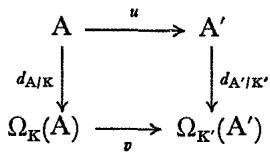
\includegraphics[keepaspectratio]{images/part004_9ff9737d.jpg}}

\(d_{\mathbf{A}^{\prime} / \mathbf{K}^{\prime}}\circ u\) 是 A 的、取值于 A-模 \(\Omega_{\mathbf{K}^{\prime}}(\mathbf{A}^{\prime})\) 的一个 K-导子； \(v\) 的存在性与唯一性随后由第11号命题18得出。

命题19中的映射 v 将记作 \(\Omega(u)\) ；若存在一个由交换环同态构成的交换图

\pandocbounded{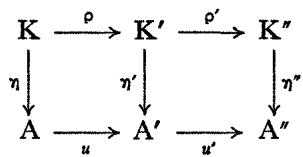
\includegraphics[keepaspectratio]{images/part004_26fbb1e8.jpg}}

由命题19的唯一性性质，立即得出

\[
\Omega (u ^ {\prime} \circ u) = \Omega (u ^ {\prime}) \circ \Omega (u).
\]

由于 \(\Omega_{\mathbf{K}'}(\mathbf{A}')\) 是一个 \(\mathbf{A}'\) -模，由 \(\Omega(u)\) 我们典范地导出一个 \(\mathbf{A}'\) -线性映射

\[
\Omega_ {0} (u): \Omega_ {\mathbf {K}} (\mathrm{A}) \otimes_ {\mathrm{A}} \mathrm{A} ^ {\prime} \rightarrow \Omega_ {\mathbf {K} ^ {\prime}} (\mathrm{A} ^ {\prime})\tag{41}
\]

，使得 \(\Omega(u)\) 是 \(\Omega_0(u)\) 与典范同态 \(i_{\mathbf{A}}: \Omega_{\mathbf{K}}(\mathbf{A}) \to \Omega_{\mathbf{K}}(\mathbf{A}) \otimes_{\mathbf{A}} \mathbf{A}'\) 的复合。对每个 \(\mathbf{A}'\) -模 \(\mathbf{E}'\) ，有一个交换图

\pandocbounded{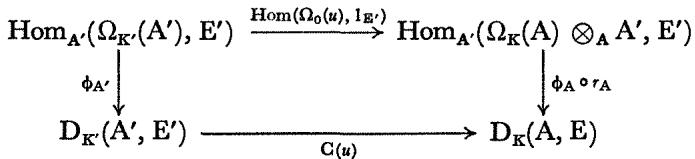
\includegraphics[keepaspectratio]{images/part004_95f64194.jpg}}

（其中 \(\mathbf{C}(u)\) 是映射 \(D \mapsto D \circ u\) （第7号，命题9），而 \(r_{A}\) 是典范同构

\[
\operatorname{Hom} \left(i _ {\mathrm{A}}, 1 _ {\mathrm{E} ^ {\prime}}\right): \operatorname{Hom} _ {\mathrm{A} ^ {\prime}} \left(\Omega_ {\mathrm{K}} (\mathrm{A}) \otimes_ {\mathrm{A}} \mathrm{A} ^ {\prime}, \mathrm{E} ^ {\prime}\right)\rightarrow \operatorname{Hom} _ {\mathrm{A}} \left(\Omega_ {\mathrm{K}} (\mathrm{A}), \mathrm{E} ^ {\prime}\right);
\]

这直接由命题19以及同构 \(\phi_{\mathbf{A}}\) 和 \(\phi_{\mathbf{A}^{\prime}}\) 的定义得出。

命题20. 假设 \(\mathbf{A}' = \mathbf{A} \otimes_{\mathbb{K}} \mathbf{K}'\) ，其中 \(\eta': \mathbf{K}' \to \mathbf{A}'\) 和 \(u: \mathbf{A} \to \mathbf{A}'\) 是典范同态。则 \(\mathbf{A}'\) -线性映射

\[
\Omega_ {0} (u): \Omega_ {\mathbf {K}} (\mathrm{A}) \otimes_ {\mathbf {A}} \mathrm{A} ^ {\prime} \rightarrow \Omega_ {\mathbf {K} ^ {\prime}} (\mathrm{A} ^ {\prime})
\]

是一个同构。

由于图(42)中竖直箭头是双射，问题归结为证明：对每个A'-模E'，图(42)中的同态C(u):D → D ∘ u是双射（II，§2，第1号，定理1）。现在Hom(u, 1\_E') : Hom\_K'(A ⊗\_K K', E') → Hom\_K(A, E')是同构（II，§5，第1号，命题1），而C(u)是它在D\_K'(A', E')上的限制，因此是单射；此外，若 f: A' → E' 是一个 K'-线性映射，使得

\[
f \circ u: \mathrm{A} \rightarrow \mathrm{E} ^ {\prime}
\]

是 K-导子，则由 \(f\) 是 \(\mathbf{K}'\) -线性的以及 \(f((x \otimes 1)(y \otimes 1)) = (y \otimes 1)f(x \otimes 1) + (x \otimes 1)f(y \otimes 1)\) （对 A 中的 \(x, y\) ）这一事实，立即得出 \(f\) 是一个 \(\mathbf{K}'\) -导子，因为元素 \(x \otimes 1\) （对 \(x \in A\) ）构成 \(\mathbf{K}'\) -模 \(A'\) 的一个生成系；这就完成了 \(C(u)\) 是双射的证明。

从现在起，我们把注意力限制在 \(\rho: \mathbf{K} \to \mathbf{K}'\) 是 \(\mathbf{K}\) 的恒等映射的情形；每个 K-代数同态 \(u: \mathbf{A} \to \mathbf{B}\) 因此被映为一个 B-线性映射

\[
\Omega_ {0} (u): \Omega_ {\mathbf {K}} (\mathrm{A}) \otimes_ {\mathbf {K}} \mathrm{B} \rightarrow \Omega_ {\mathbf {K}} (\mathrm{B}).\tag{43}
\]

另一方面，我们可以考虑 A-微分的 B-模 \(\Omega_{\mathbf{A}}(\mathbf{B})\) ，因为 B 通过 u 成为 A-代数；典范导子 \(d_{\mathrm{B/A}}: \mathbf{B} \to \Omega_{\mathbf{A}}(\mathbf{B})\) 当然更是 K-导子，因此它唯一地分解为

\[
\mathbf {B} \xrightarrow {d _ {\mathbf {B} / \mathbf {K}}} \Omega_ {\mathbf {K}} (\mathbf {B}) \xrightarrow {\Omega_ {u}} \Omega_ {\mathbf {A}} (\mathbf {B})
\]

其中 \(\Omega_{u}\) 是 B-线性映射（第11号，命题18）。对每个 B-模 E，有交换图

\[
\begin{array}{c} \operatorname{Hom} _ {\mathbf {B}} (\Omega_ {\mathbf {A}} (\mathbf {B}), \mathrm{E}) \xrightarrow {\operatorname{Hom} (\Omega_ {u} , 1 _ {\mathbf {E}})} \operatorname{Hom} _ {\mathbf {B}} (\Omega_ {\mathbf {K}} (\mathbf {B}), \mathrm{E}) \\ \phi_ {\mathbf {A}, \mathbf {B}} \Biggl \downarrow \\ \mathrm{D} _ {\mathbf {A}} (\mathrm{B}, \mathrm{E}) \xrightarrow [ j _ {u} ]{} \mathrm{D} _ {\mathbf {K}} (\mathrm{B}, \mathrm{E}) \end{array}\tag{44}
\]

其中 \(j_{u}\) 是典范单射（第7号）；这直接由第11号的命题18得出。

命题21：B-线性映射的序列

\[
\Omega_ {\mathbf {K}} (\mathrm{A}) \otimes_ {\mathbf {A}} \mathrm{B} \xrightarrow {\Omega_ {0} (u)} \Omega_ {\mathbf {K}} (\mathrm{B}) \xrightarrow {\Omega_ {u}} \Omega_ {\mathbf {A}} (\mathrm{B}) \to 0\tag{45}
\]

是正合的。

只需验证：对每个B-模E，序列

\[
\begin{array}{c} 0 \to \operatorname{Hom} _ {\mathrm{B}} (\Omega_ {\mathrm{A}} (\mathrm{B}), \mathrm{E}) \xrightarrow {\operatorname{Hom} (\Omega_ {\mathrm{u}} , 1 _ {\mathrm{E}})} \operatorname{Hom} _ {\mathrm{B}} (\Omega_ {\mathrm{K}} (\mathrm{B}), \mathrm{E}) \\ \xrightarrow {\operatorname{Hom} (\Omega_ {0} (u) , 1 _ {\mathrm{E}})} \operatorname{Hom} _ {\mathrm{B}} (\Omega_ {\mathrm{K}} (\mathrm{A}) \otimes_ {\mathrm{A}} \mathrm{B}, \mathrm{E}) \end{array}
\]

是正合的（II，§2，第1号，定理1）；但由于在交换图（42）和（44）中垂直箭头是同构的，只需证明序列

\[
0 \longrightarrow \mathrm{D} _ {\mathrm{A}} (\mathrm{B}, \mathrm{E}) \xrightarrow {j _ {u}} \mathrm{D} _ {\mathrm{K}} (\mathrm{B}, \mathrm{E}) \xrightarrow {\mathrm{C} (u)} \mathrm{D} _ {\mathrm{K}} (\mathrm{A}, \mathrm{E})
\]

是正合的，这正是第7号的命题11。

现在我们考虑 K-代数同态 \(u: \mathbf{A} \to \mathbf{B}\) 是满射的情形；若 \(\mathfrak{J}\) 是其核，则 \(\mathbf{B}\) 同构于 \(\mathbf{A} / \mathfrak{J}\) 。我们考虑典范导子的限制 \(d| \mathfrak{J}: \mathfrak{J} \to \Omega_{\mathbf{K}}(\mathbf{A})\) （其中 \(d = d_{\mathbf{A} / \mathbf{K}}\) ）以及复合 A-线性映射

\[
d ^ {\prime}: \mathfrak {J} \xrightarrow {d | \mathfrak {J}} \Omega_ {\mathrm{K}} (\mathrm{A}) \xrightarrow {i _ {\mathrm{A}}} \Omega_ {\mathrm{K}} (\mathrm{A}) \otimes_ {\mathrm{A}} \mathrm{B}.
\]

那么 \(d^{\prime}(\mathfrak{J}^{2}) = 0\) ，因为，对于 \(x, y\) 在 \(\mathfrak{J}\) ,

\[
d ^ {\prime} (x y) = d (x y) \otimes 1 = (x. d y + y. d x) \otimes 1 = d y \otimes u (x) + d x \otimes u (y) = 0
\]

因为 \(u(x) = u(y) = 0\) 。因此我们由 \(d'\) 通过过渡到商得到一个 A-线性映射

\[
\bar {d} \colon \mathfrak {J} / \mathfrak {J} ^ {2} \rightarrow \Omega_ {\mathrm{K}} (\mathrm{A}) \otimes_ {\mathrm{A}} \mathrm{B}
\]

且由于 \(\mathfrak{J}\) 零化 A-模 \(\mathfrak{J} / \mathfrak{J}^2\) ， \(\bar{d}\) 是一个 B-线性映射。

命题 22。设 \(\mathfrak{J}\) 是交换 K-代数 A 的一个理想，B = A/ \(\mathfrak{J}\) ， \(u:A\to B\) 为典范同态。B-线性映射的序列

\[
\mathfrak {J} / \mathfrak {J} ^ {2} \xrightarrow {\overline {{d}}} \Omega_ {\mathrm{K}} (\mathrm{A}) \otimes_ {\mathrm{A}} \mathrm{B} \xrightarrow {\Omega_ {0} (u)} \Omega_ {\mathrm{K}} (\mathrm{B}) \to 0\tag{46}
\]

因而是正合的。

注意， \(\Omega_{\mathbf{K}}(\mathbf{A}) \otimes_{\mathbf{A}} \mathbf{B}\) 与 \(\Omega_{\mathbf{K}}(\mathbf{A}) / \mathfrak{J} \Omega_{\mathbf{K}}(\mathbf{A})\) 相等同，且 \(\bar{d}\) 的像就是 \(d(\mathfrak{J})\) 在这个商模中的像； \(\Omega_{\mathbf{K}}(\mathbf{A}) \otimes_{\mathbf{A}} \mathbf{B}\) 关于 \(\operatorname{Im}(\bar{d})\) 的商因此等同于商 \(\Omega_{\mathbf{K}}(\mathbf{A}) / \mathbf{N}\) ，其中 \(\mathbf{N}\) 是由 \(\mathfrak{J} \Omega_{\mathbf{K}}(\mathbf{A})\) 和 \(d(\mathfrak{J})\) 生成的子 A-模。此外，复合映射

\[
\mathrm{A} \xrightarrow {d _ {\mathrm{A} / \mathrm{K}}} \Omega_ {\mathrm{K}} (\mathrm{A}) \longrightarrow \Omega_ {\mathrm{K}} (\mathrm{A}) / \mathrm{N}
\]

是一个 K-导子（第7号，命题9），并且由于它在 \(\mathfrak{J}\) 上为零（根据 N 的定义），当过渡到商时，它定义了一个 K-导子 \(D_0:B\to \Omega_{\mathbb{K}}(A) / N\) .

考虑到泛映射问题解的唯一性，可以归结为证明：对于每个 B-模 E 和每个 K-导子 D: B → E，存在唯一的 B-线性映射 g： \(\Omega_{\mathrm{K}}(\mathrm{A})/\mathrm{N} \rightarrow \mathrm{E}\) ，使得 \(D = g \circ D_{0}\) 。但是，复合映射 D ∘ u: A → E 是一个 K-导子（第7号，命题9），因此存在且仅存在一个 A-线性映射 f： \(\Omega_{\mathrm{K}}(\mathrm{A}) \rightarrow \mathrm{E}\) ，使得 \(f \circ d_{A/K} = D \circ u\) 。这个关系式已经表明 f 在 \(d(\mathfrak{J})\) 上为零；又因为 E 是 B-模， \(\mathfrak{J} E = \{0\}\) ，所以 f 在 \(\mathfrak{J} \Omega_{\mathrm{K}}(\mathrm{A})\) 上为零；因此 f 在 N 上为零，并在取商后定义了一个 B-线性映射 g： \(\Omega_{\mathrm{K}}(\mathrm{A})/\mathrm{N} \rightarrow \mathrm{E}\) ，使得 \(g \circ D_{0} = D\) ；g 的唯一性由 f 的唯一性得出。

不要以为，即使 \(u: \mathbf{A} \to \mathbf{B}\) 是单射同态， \(\Omega_0(u): \Omega_{\mathbf{K}}(\mathbf{A}) \otimes_{\mathbf{A}} \mathbf{B} \to \Omega_{\mathbf{K}}(\mathbf{B})\) 也是单射（练习5）。然而我们有如下命题：

命题23。设 A 是一个整 K-代数，B 是其分式域，且 \(u: \mathbf{A} \to \mathbf{B}\) 为典范单射。则 \(\Omega_0(u): \Omega_{\mathbf{K}}(\mathbf{A}) \otimes_{\mathbf{A}} \mathbf{B} \to \Omega_{\mathbf{K}}(\mathbf{B})\) 是一个同构。

利用图(42)中竖直箭头是双射这一事实，问题归结为证明：对于B上的每一个向量空间E，映射 \(\mathrm{C}(u):\mathrm{D}_{\mathrm{K}}(\mathrm{B},\mathrm{E})\to\mathrm{D}_{\mathrm{K}}(\mathrm{A},\mathrm{E})\) 是双射。但这可由以下事实推出：A到E的每一个K-导子都能唯一地延拓为B到E的K-导子（第5号，命题5）。

\section{余代数、多重线性形式的乘积、内乘与对偶}

在本段中，A 是带平凡分次的交换环。对 N 型分次 A-模 M， \(M^{*gr}\) 表示这样的 N 型分次 A-模：其 n 次齐次元素是在 \(M_{k}\) 上（对所有 \(k \neq n\) ）为零的那些 A-线性形式。

\subsection{余代数}

定义 1. A 上的余代数（或 A-余代数，若不致混淆则简称为余代数）是一个集合 E，其结构由给出以下内容来定义：

\begin{enumerate}
\def\labelenumi{(\arabic{enumi})}
\item
  E 上的一个 A-模结构；
\item
  一个 A-线性映射 \(c: \mathbf{E} \to \mathbf{E} \otimes_{\mathbf{A}} \mathbf{E}\) ，称为 \(\mathbf{E}\) 的余积。
\end{enumerate}

定义2. 给定两个余代数E、E'，其余积分别记为c和c'，从E到E'的一个态射是一个A-线性映射u：E → E'，使得

\[
(u \otimes u) \circ c = c ^ {\prime} \circ u\tag{1}
\]

换言之，它使得A-线性映射的图表可交换

\pandocbounded{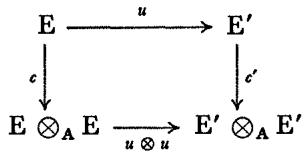
\includegraphics[keepaspectratio]{images/part004_6ed4336b.jpg}}

立即可以验证，恒等映射是态射，两个态射的复合是态射，并且每个双射态射都是同构。

示例。（1）典范同构 \(\mathbf{A} \to \mathbf{A} \otimes_{\mathbf{A}} \mathbf{A}\) (II, § 3, 第 5 号) 在 \(\mathbf{A}\) 上定义了一个 A-余代数结构。

\begin{enumerate}
\def\labelenumi{(\arabic{enumi})}
\setcounter{enumi}{1}
\item
  设 E 为一个余代数，c 为其余积，且 \(\sigma\) 为 A-模 \(E \otimes_{A} E\) 的典范自同构，使得 \(\sigma(x \otimes y) = y \otimes x\) （对 \(x \in E\) , \(y \in E\) ）；A-线性映射 \(\sigma \circ c\) 在 E 上定义了一个新的余代数结构。带此结构的 E 称为给定余代数 E 的反余代数。
\item
  设 B 为一个 A-代数，并设 \(m:B \otimes_{A} B \to B\) 为定义 B 上乘法的 A-线性映射（ \(\S 1\) ，第3号）。转置 \(^{t}m\) 于是是从 A-模 B 的对偶 \(B^{*}\) 到 \((\mathbf{B} \otimes_{\mathbf{A}} \mathbf{B})^{*}\) （即 A-模 \(B \otimes_{A} B\) 的对偶）中的一个 A-线性映射。若 B 还是有限生成的投射 A-模，则典范映射 \(\mu:B^{*} \otimes_{A} B^{*} \to (\mathbf{B} \otimes_{\mathbf{A}} \mathbf{B})^{*}\) 是一个 A-模同构（II， \(\S 4\) ，第4号）；映射 \(c = \mu^{-1} \circ ^{t}m\) 于是是一个余积，它在 A-模 B 的对偶 \(B^{*}\) 上定义了一个余代数结构。
\item
  设 X 是一个集合， \(\mathbf{A}^{(\mathbf{X})}\) 是 X 中元素以 A 中系数构成的形式线性组合的 A-模（II，§1，第11号），且 \((e_{x})_{x\in\mathbf{X}}\) 是 \(\mathbf{A}^{(\mathbf{X})}\) 的典范基。A-线性映射 \(c:A^{(\mathbf{X})}\to\mathbf{A}^{(\mathbf{X})}\otimes_{\mathbf{A}}\mathbf{A}^{(\mathbf{X})}\) 由条件 \(c(e_{x})=e_{x}\otimes e_{x}\) 定义，从而在 \(\mathbf{A}^{(\mathbf{X})}\) 上得到了一个典范余代数结构。
\item
  设 \(\mathbf{M}\) 是一个 A-模，且 \(\mathsf{T}(\mathbf{M})\) 是 \(\mathbf{M}\) 的张量代数 ( \(\S 5\) ，第1号）；根据 II， \(\S 3\) 第9号，存在且仅存在一个 A-线性映射 \(c\) ，它从 A-模 \(\mathsf{T}(\mathbf{M})\) 到 A-模 \(\mathsf{T}(\mathbf{M}) \otimes_{\mathbf{A}} \mathsf{T}(\mathbf{M})\) 中，使得对所有 \(n \geqslant 0\) ，
\end{enumerate}

\[
c (x _ {1} x _ {2} \dots x _ {n}) = \sum_ {0 \leqslant p \leqslant n} (x _ {1} x _ {2} \dots x _ {p}) \otimes (x _ {p + 1} \dots x _ {n})\tag{3}
\]

对所有 \(x_{i} \in \mathbf{M}\) ( \(x_{1}x_{2}\ldots x_{n}\) 表示代数 \(\mathsf{T}(\mathbf{M})\) 中的乘积）。这样， \(\mathsf{T}(\mathbf{M})\) 就被赋予了余代数结构。

\begin{enumerate}
\def\labelenumi{(\arabic{enumi})}
\setcounter{enumi}{5}
\tightlist
\item
  设 M 是一个 A-模，S(M) 是 M 的对称代数（§ 6，第 1 号）；从 M 到 M × M 的对角映射 \(\Delta: x \mapsto (x, x)\) 是一个 A-线性映射，因此对应着从 A-代数 S(M) 到 A-代数 S(M × M) 的一个同态 S(Δ)（§ 6，第 2 号，命题 3）。另一方面，在 § 6，第 6 号中我们定义了一个典范分次代数同构 \(h \colon \mathbb{S}(\mathbf{M} \times \mathbf{M}) \to \mathbb{S}(\mathbf{M}) \otimes_{\mathbf{A}} \mathbb{S}(\mathbf{M})\) ；通过复合，我们因此得到一个 A-代数同态
\end{enumerate}

\[
c = h \circ \mathbf {S} (\Delta): \mathbf {S} (\mathbf {M}) \rightarrow \mathbf {S} (\mathbf {M}) \otimes_ {\mathbf {A}} \mathbf {S} (\mathbf {M}),
\]

从而在 \(\mathbf{S}(\mathbf{M})\) 上定义了一个余代数结构。对所有 \(x\in \mathbf{M}\) ，根据定义 \(\mathbf{S}(\Delta)(x) = (x,x)\) ，而 § 6 第6号中给出的 \(h\) 的定义表明

\[
h ((x, x)) = x \otimes 1 + 1 \otimes x.
\]

由此可得 \(c\) 是唯一的代数同态，使得对所有 \(x \in \mathbf{M}\) ,

\[
c (x) = x \otimes 1 + 1 \otimes x.\tag{4}
\]

由于 \(c\) 是一个代数同态，因此得出：对每个序列 \((x_{i})_{1\leqslant i\leqslant n}\) （ \(n\) 个元素取自 \(\mathbf{M}\) ），

\[
\begin{array}{r l} c (x _ {1} x _ {2} \dots x _ {n}) & = \prod_ {i = 1} ^ {n} (x _ {i} \otimes 1 + 1 \otimes x _ {i}) \\ & = \sum (x _ {i _ {1}} \dots x _ {i _ {p}}) \otimes (x _ {j _ {1}} \dots x _ {j _ {n - p}}) \end{array}\tag{5}
\]

（5）式右端的求和是对所有严格递增序列（在某些情况下为空）的有序对进行的

\[
i _ {1} <   i _ {2} <   \dots <   i _ {p}, \quad j _ {1} <   j _ {2} <   \dots <   j _ {n - p}
\]

的元素组成 \([1, n]\) ，且其元素集合互补。元素 \(c(x_1 x_2 \ldots x_n)\) 是总次数为 \(n\) 的、 \(\mathbb{S}(\mathbf{M}) \otimes_{\mathbf{A}} \mathbb{S}(\mathbf{M})\) 中的元素，其双次数为 \((p, n - p)\) 的分量是

\[
\sum_ {\sigma} \left(x _ {\sigma (1)} \dots x _ {\sigma (p)}\right) \otimes \left(x _ {\sigma (p + 1)} \dots x _ {\sigma (n)}\right)\tag{6}
\]

其中求和遍历所有排列 \(\sigma\in\mathbb{S}_{n}\) ，这些排列在每个区间 \([1,p]\) 和 \([p+1,n]\) 上都是递增的。

\begin{enumerate}
\def\labelenumi{(\arabic{enumi})}
\setcounter{enumi}{6}
\tightlist
\item
  设 \(\mathbf{M}\) 是一个 A-模，对外代数 \(\bigwedge (\mathbf{M})\) 按照例 6 中对 \(\mathbb{S}(\mathbf{M})\) 的方式处理；对角映射 \(\Delta : \mathbf{M} \to \mathbf{M} \times \mathbf{M}\) 这次定义了同态 \(\bigwedge (\Delta)\) ，它从 A-代数 \(\bigwedge (\mathbf{M})\) 到 A-代数 \(\bigwedge (\mathbf{M} \times \mathbf{M})\) 中（§7，第2号，命题2）；另一方面，存在典范分次代数同构
\end{enumerate}

\[
h: \bigwedge (\mathbf {M} \times \mathbf {M}) \rightarrow \bigwedge (\mathbf {M}) ^ {\mathrm{g}} \otimes_ {\mathbf {A}} \bigwedge (\mathbf {M})
\]

（§7，第7号，命题10），因此通过复合得到代数同态 \(c = h \circ \bigwedge(\Delta): \bigwedge(M) \to \bigwedge(M)^{\mathfrak{g}} \otimes_{A} \bigwedge(M)\) ，它可视为 A-模同态 \(\bigwedge(M) \to \bigwedge(M) \otimes_{A} \bigwedge(M)\) ，从而在 \(\bigwedge(M)\) 上定义了一个余代数结构。可如同例 6 那样证明 \(c\) 是唯一的代数同态，使得对所有 \(x \in M\) ，

\[
c (x) = x \otimes 1 + 1 \otimes x,\tag{7}
\]

，因此，对每个序列 \((x_{i})_{1\leqslant i\leqslant n}\) （元素属于 \(\mathbf{M}\) ），

\[
c \left(x _ {1} \wedge x _ {2} \wedge \dots \wedge x _ {n}\right) = \left(x _ {1} \otimes 1 + 1 \otimes x _ {1}\right) \wedge \dots \wedge \left(x _ {n} \otimes 1 + 1 \otimes x _ {n}\right)
\]

其中右侧的乘积是在代数中进行的

\[
\Lambda (\mathbf {M}) ^ {\mathfrak {g}} \otimes_ {\mathbf {A}} \Lambda (\mathbf {M});
\]

为了计算这个乘积，对每对严格递增序列 \(i_1 < i_2 < \cdots < i_p\) , \(j_1 < j_2 < \cdots < j_{n-p}\) （由 \([1, n]\) 的元素组成，且其元素集合互补），考虑乘积 \(y_1y_2\ldots y_n\) ，其中 \(y_{i_h} = x_{i_h} \otimes 1 (1 \leqslant h \leqslant p)\) 和 \(y_{j_k} = 1 \otimes x_{j_k} (1 \leqslant k \leqslant n - p)\) 并且求和是对所有这些乘积进行的。由于分次代数 \(\bigwedge (\mathbf{M})^{\mathfrak{g}} \otimes_{\mathbf{A}} \bigwedge (\mathbf{M})\) 是反交换的，且元素 \(x_i \otimes 1\) 和 \(1 \otimes x_i\) 的总次数为1，根据§4，第6号，引理3和引理1，

\[
\begin{array}{r l} c (x _ {1} \wedge x _ {2} \wedge \dots \wedge x _ {n}) & = \sum (- 1) ^ {\nu} (x _ {i _ {1}} \wedge \dots \wedge x _ {i _ {p}}) \otimes (x _ {j _ {1}} \wedge \dots \wedge x _ {j _ {n - p}}) \end{array} \tag {8}
\]

其中 v 是有序对 \((h, k)\) 的个数，这些对满足 \(j_{k} < i_{h}\) ，且求和范围与 (5) 中相同。元素 \(c(x_{1} \wedge \cdots \wedge x_{n})\) 在 \(\bigwedge(\mathbf{M})^{\mathbf{g}} \otimes_{\mathbf{A}} \bigwedge(\mathbf{M})\) 中的总次数为 n，其双次数 \((p, n - p)\) 的齐次分量等于

\[
\sum_ {\sigma} \varepsilon_ {\sigma} (x _ {\sigma (1)} \wedge \dots \wedge x _ {\sigma (p)}) \otimes (x _ {\sigma (p + 1)} \wedge \dots \wedge x _ {\sigma (n)})\tag{9}
\]

求和遍历所有置换 \(\sigma\in\mathfrak{S}_{n}\) ，它们在每个区间 \([1,p]\) 和 \([p+1,n]\) 上都是递增的。

今后当我们谈到 \(\mathbf{A}^{(\mathbf{X})}\) , \(\mathsf{T}(\mathbf{M})\) , \(\mathsf{S}(\mathbf{M})\) 或 \(\bigwedge (\mathbf{M})\) 作为余代数时，除非另有说明，我们指的是分别在例 4、5、6 和 7 中定义的余代数结构。

\begin{enumerate}
\def\labelenumi{(\arabic{enumi})}
\setcounter{enumi}{7}
\tightlist
\item
  设 E, F 为两个 A-余代数，c, \(c'\) 分别为其余积。设 \(\tau:(\mathbf{E} \otimes_{\mathbf{A}} \mathbf{E}) \otimes_{\mathbf{A}} (\mathbf{F} \otimes_{\mathbf{A}} \mathbf{F}) \to (\mathbf{E} \otimes_{\mathbf{A}} \mathbf{F}) \otimes_{\mathbf{A}} (\mathbf{E} \otimes_{\mathbf{A}} \mathbf{F})\) 表示结合性同构，使得 \(\tau((x \otimes x') \otimes (y \otimes y')) = (x \otimes y) \otimes (x' \otimes y')\) 对 E 中的 \(x, x'\) 和 F 中的 \(y, y'\) 成立。则复合线性映射
\end{enumerate}

\[
\mathrm{E} \otimes_ {\mathrm{A}} \mathrm{F} \xrightarrow {c \otimes c ^ {\prime}} (\mathrm{E} \otimes_ {\mathrm{A}} \mathrm{E}) \otimes_ {\mathrm{A}} (\mathrm{F} \otimes_ {\mathrm{A}} \mathrm{F}) \xrightarrow {\tau} (\mathrm{E} \otimes_ {\mathrm{A}} \mathrm{F}) \otimes_ {\mathrm{A}} (\mathrm{E} \otimes_ {\mathrm{A}} \mathrm{F})
\]

在 A-模 E \(\otimes_{\mathbf{A}}\mathbf{F}\) 上定义了一个余代数结构，称为余代数 E 和 F 的张量积。

设 E 为一个余代数， \(\Delta\) 为一个交换幺半群。A-模 E 上的分次 \((\mathrm{E}_{\lambda})_{\lambda\in\Delta}\) 称为与 E 的余积 c 相容，如果 c 是从分次 A-模 E 到分次 A-模（ \(\Delta\) 型的 \(E\otimes_{A}E\) ）中的 0 次分次同态，换言之（II，§11，第 5 号），如果

\[
\mathrm{c} (\mathrm{E} _ {\lambda}) \subset \sum_ {\mu + \nu = \lambda} \mathrm{E} _ {\mu} \otimes_ {\mathbf {A}} \mathrm{E} _ {\nu}.\tag{10}
\]

在下文中，我们通常将注意力限制在与余积相容的 N 型分次上；带有这种分次的余代数也称为分次余代数。若 F 是另一个分次余代数，则分次余代数态射 \(\phi:E\to F\) 按定义是一个余代数态射（定义 2），同时也是分次 A-模之间的 0 次分次同态。

例。（9）显然，上述定义的余代数 \(\mathsf{T}(\mathbf{M})\) , \(\mathsf{S}(\mathbf{M})\) 和 \(\bigwedge (\mathbf{M})\) 都是分次余代数。

\subsection{余结合性、余交换性、余单位}

设 E 为一个余代数，c 为其余积，N, N', N'' 为三个 A-模，m 为 N × N' 到 N'' 的一个双线性映射。设 \(\tilde{m}:N \otimes_{A} N' \to N''\) 为对应于 m 的 A-线性映射。若 \(u:E \to N\) , \(v:E \to N'\) 是两个 A-线性映射，我们得到一个 A-线性映射 \(u \otimes v:E \otimes_{A} E \to N \otimes_{A} N'\) 以及一个从 E 到 N'' 的复合 A-线性映射：

\[
m (u, v): \mathrm{E} \xrightarrow {c} \mathrm{E} \otimes_ {\mathrm{A}} \mathrm{E} \xrightarrow {u \otimes v} \mathrm{N} \otimes_ {\mathrm{A}} \mathrm{N} ^ {\prime} \xrightarrow {\tilde {m}} \mathrm{N} ^ {\prime \prime}.\tag{11}
\]

显然，我们由此定义了一个 A-双线性映射 \((u, v) \mapsto m(u, v)\) ，它从 \(\operatorname{Hom}_{\mathbf{A}}(\mathbf{E}, \mathbf{N}) \times \operatorname{Hom}_{\mathbf{A}}(\mathbf{E}, \mathbf{N}')\) 到 \(\operatorname{Hom}_{\mathbf{A}}(\mathbf{E}, \mathbf{N}'')\) 中。

当 E 为分次余代数，N, N', N'' 为同类型的分次 A-模，且 \(\tilde{m}\) 为从 N \(\otimes_{A}N'\) 到 N'' 的 k 次分次同态时，若 u（相应地 v）是 p 次（相应地 q 次）分次同态，则 \(m(u,v)\) 是次数为 \(p + q + k\) 的分次同态。

例。（1）取 E 为分次余代数 T(M)（第 1 号），并假设 N, N', N'' 具有平凡分次。则从 T(M) 到 N（相应地 N', N''）的 -p 次分次同态对应于从 M\^{}p 到 N（相应地 N', N''）的多重线性映射。给定一个多重线性映射 u: M\^{}p → N 和一个多重线性映射 v: M\^{}q → N'，上述方法使我们能够推导出一个多重线性映射 m(u, v)：M\^{}\{p+q\} → N''，称为u与v的（关于m的）乘积。公式（3）（第1号）和（11）表明，对于M中的x\_1, . . ., x\_p+q，

\[
(m (u, v)) \left(x _ {1}, \dots , x _ {p + q}\right) = m \left(u \left(x _ {1}, \dots , x _ {p}\right), v \left(x _ {p + 1}, \dots , x _ {p + q}\right)\right).
\]

\begin{enumerate}
\def\labelenumi{(\arabic{enumi})}
\setcounter{enumi}{1}
\tightlist
\item
  设 E 为分次余代数 S(M)（第 1 号），对 N、N'、N'' 保持相同的假设。从 S(M) 到 N 的 −p 次分次同态对应于从 M \(^{p}\) 到 N 的对称多重线性映射（§ 6，第 3 号）。于是，由对称多重线性映射 u: M \(^{p}\) → N 和对称多重线性映射 v: M \(^{q}\) → N' 得到一个对称多重线性映射 m(u, v)：M \(^{p+q}\) → N''，也（为避免混淆）记作 \(u \cdot_{m} v\) （甚至 \(u \cdot v\)），并称为 u 和 v 的（关于 m 的）对称积。公式 (6)（第 1 号）和 (11) 表明，对于 M 中的 x₁， \ldots， \(_{p+q}\) ，
\end{enumerate}

\[
(u \cdot_{m} v) (x _ {1}, \dots , x _ {p + q}) = \sum_ {\sigma} m (u (x _ {\sigma (1)}, \dots , x _ {\sigma (p)}), v (x _ {\sigma (p + 1)}, \dots , x _ {\sigma (p + q)}))
\]

求和遍历所有置换 \(\sigma\in\mathfrak{S}_{p+q}\) ，这些置换在每个区间 \([1,p]\) 和 \([p+1,p+q]\) 上都是递增的。

\begin{enumerate}
\def\labelenumi{(\arabic{enumi})}
\setcounter{enumi}{2}
\tightlist
\item
  取 E 为分次余代数 \(\bigwedge (\mathbf{M})\) （第 1 号）。于是我们类似地从交错多重线性映射 \(u: \mathbf{M}^p \to \mathbf{N}\) 和交错多重线性映射 \(v: \mathbf{M}^q \to \mathbf{N}'\) 得到一个交错多重线性映射 \(m(u, v): \mathbf{M}^{p + q} \to \mathbf{N}''\) ，也记作 \(u \wedge_m v\) 或 \(u \wedge v\) ，并称为（关于 \(m\) 的） \(u\) 和 \(v\) 的交错积。公式（9）（第 1 号）和（11）表明在这种情况下，对于 \(x_1, \ldots, x_{p + q}\) （在 \(\mathbf{M}\) 中），
\end{enumerate}

\[
(u \wedge_ {m} v) (x _ {1}, \dots , x _ {p + q}) = \sum_ {\sigma} \varepsilon_ {\sigma} m (u (x _ {\sigma (1)}, \dots , x _ {\sigma (p)}), v (x _ {\sigma (p + 1)}, \dots , x _ {\sigma (p + q)}))
\]

求和再次遍历所有排列 \(\sigma \in \mathfrak{S}_{p + q}\) ，这些排列在每个区间 \([1, p]\) 和 \([p + 1, p + q]\) 上都是递增的。

我们回到 E 为任意分次余代数（N 型）的情形，并假设三个模 N、N'、N'' 都等于一个 Z 型分次 A-代数 B 的底层 A-模，映射 m 为 B 中的乘法，从而 \(\tilde{m}:B\otimes_{A}B\to B\) 是一个次数为 0 的分次 A-线性映射。于是在分次 A-模 \(\operatorname{Homgr}_{A}(E,B)=C\) 上获得了一个分次 A-代数结构。

特别地，假设 B = A（具有平凡分次），因此 \(\operatorname{Homgr}_{\mathbf{A}}(\mathbf{E}, \mathbf{A})\) 是分次对偶 \(E^{*gr}\) ，从而它具有一个分次 A-代数结构。

设 F 为另一个分次余代数， \(c'\) 为其余积， \(\phi:E\to F\) 为一个分次余代数态射（第1号）；则典范分次态射

\[
\tilde {\phi} = \operatorname{Hom} (\phi , 1 _ {B}): \operatorname{Homgr} _ {A} (F, B) \rightarrow \operatorname{Homgr} _ {A} (E, B)
\]

是一个分次代数同态。对于 \(u, v\) 在 \(\operatorname{Homgr}_{\mathbf{A}}(\mathbf{F}, \mathbf{B})\) 和 \(x \in \mathbf{E}\) ,

\[
(\tilde {\phi} (u v)) (x) = (u v) (\phi (x)) = m ((u \otimes v) (c ^ {\prime} (\phi (x))))
\]

但根据假设 \(c'(\phi(x)) = (\phi \otimes \phi)(c(x))\) ，因此

\[
(u \otimes v) (c ^ {\prime} (\phi (x))) = (\tilde {\phi} (u) \otimes \tilde {\phi} (v)) (c (x))
\]

，从而 \(\tilde{\phi}(uv) = \tilde{\phi}(u)\tilde{\phi}(v)\) ，这证明了我们的断言。

特别地，分次转置 \({}^{t}\phi: \mathrm{F}^{*gr} \to \mathrm{E}^{*gr}\) 是分次代数同态。

注：假设诸 \(E_{p}\) 是有限生成的投射 A-模，因此分次 A-模（ \(E \otimes_{A} E)^{*gr}\) 和 \(E^{*gr} \otimes_{A} E^{*gr}\) 可以典范地等同（II，§4，第4号，命题4的推论1）。如果 A-模 \(A \otimes_{A} A\) 和 A 也被典范地等同（II，§3，第4号），则线性映射 \(E^{*gr} \otimes_{A} E^{*gr} \to E^{*gr}\) （它定义了 \(E^{*gr}\) 中的乘法）可称为余积 c 的分次转置。

命题1. 设 E 是 A 上的余代数。为使对每个结合 A-代数 B，A-代数 \(\operatorname{Hom}_{\mathbf{A}}(\mathbf{E}, \mathbf{B})\) 是结合的，其充分必要条件是余积 \(c: \mathbf{E} \to \mathbf{E} \otimes_{\mathbf{A}} \mathbf{E}\) 使得图表

\begin{enumerate}
\def\labelenumi{(\arabic{enumi})}
\setcounter{enumi}{11}
\tightlist
\item
\end{enumerate}

\pandocbounded{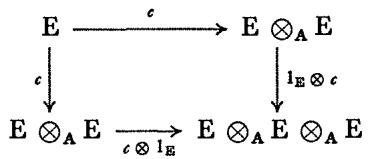
\includegraphics[keepaspectratio]{images/part004_a79ed2ff.jpg}}

是交换的。

设 B 是一个结合 A-代数，且 u、v、w 是 \(\mathbf{C} = \operatorname{Hom}_{\mathbf{A}}(\mathbf{E}, \mathbf{B})\) 的三个元素。设 \(m_{3}\) 表示 A-线性映射 \(B \otimes_{A} B \otimes_{A} B \to B\) ，它把 \(b \otimes b' \otimes b''\) 映为 \(bb'b''\) 。根据代数 C 上乘积的定义， \((uv)w\) 是复合映射

\[
\mathrm{E} \xrightarrow {c} \mathrm{E} \otimes \mathrm{E} \xrightarrow {c \otimes 1 _ {\mathrm{E}}} \mathrm{E} \otimes \mathrm{E} \otimes \mathrm{E} \xrightarrow {u \otimes v \otimes w} \mathrm{B} \otimes \mathrm{B} \otimes \mathrm{B} \xrightarrow {m _ {3}} \mathrm{B}
\]

而 \(u(vw)\) 是复合映射，

\[
\mathrm{E} \xrightarrow {c} \mathrm{E} \otimes \mathrm{E} \xrightarrow {1 _ {\mathrm{E}} \otimes c} \mathrm{E} \otimes \mathrm{E} \otimes \mathrm{E} \xrightarrow {u \otimes v \otimes w} \mathrm{B} \otimes \mathrm{B} \otimes \mathrm{B} \xrightarrow {m _ {3}} \mathrm{B}.
\]

由此可知，若图表 (12) 可交换，则代数 \(\operatorname{Hom}_{\mathbf{A}}(\mathbf{E}, \mathbf{B})\) 对每个结合的A-代数B都是结合的。为建立其逆命题，只需证明存在一个结合的A-代数B以及三个A-线性映射 \(u, v, w\) 将E映入B，使得该映射 \(m_3 \circ (u \otimes v \otimes w)\) 从 \(\mathbf{E} \otimes \mathbf{E} \otimes \mathbf{E}\) 到 B 中是单射。取 B 为 A-代数 \(\mathsf{T}(\mathbf{E})\) ， \(u, v, w\) 为 E 到 \(\mathsf{T}(\mathbf{E})\) 的典范映射。该映射 \(m_3 \circ (u \otimes v \otimes w)\) 就是典范映射 \(\mathbf{E} \otimes \mathbf{E} \otimes \mathbf{E} = \mathsf{T}^3(\mathbf{E}) \to \mathsf{T}(\mathbf{E})\) ，它是单射的。

当余代数 E 满足命题 1 的条件时，称其为余结合的。

例子。(4) 容易直接验证，余代数 A（第 1 号，例 (1)）以及余代数 \(\mathbf{A}^{(\mathbf{X})}\) （第1号，例4）和余代数 \(\mathbf{T}(\mathbf{M})\) （第1号，例5）是余结合的。若B是一个结合A-代数，且是有限生成的投射A-模，则余代数 \(\mathbf{B}^*\) （第1号，例3）是余结合的：因为此时图(12)的交换性可由表达B的结合性的图的交换性通过转置得到（ \(\S\) 1，第3号）。反之，同样的论证以及 A-模 B 与其双对偶的典范等同（II，§2，第7号，命题13的推论4）表明，若余代数 \(\mathbf{B}^*\) 是余结合的，则代数 \(\mathbf{B}\) 是结合的。最后，余代数 \(\mathsf{S}(\mathbf{M})\) 和 \(\bigwedge (\mathbf{M})\) （第1号，例6和7）是余结合的；这由图

\[
\begin{array}{c} \mathrm{M} \xrightarrow {\Delta} \mathrm{M} \times \mathrm{M} \\ \Delta \Biggl \downarrow \\ \mathrm{M} \times \mathrm{M} \xrightarrow [ \Delta \times 1 _ {\mathrm{M}} ]{} \mathrm{M} \times \mathrm{M} \times \mathrm{M} \end{array}
\]

的交换性以及 \(\mathsf{S}(\mathbf{M})\) ( \(\S 6\) ，第2号）和 \(\bigwedge (\mathbf{M})\) ( \(\S 7\) ，第2号）的函子性质得出，它们给出相应的交换图

\[
\left\{ \begin{array}{c} \mathsf {S} (\mathbf {M}) \xrightarrow {\mathsf {S} (\Delta)} \mathsf {S} (\mathbf {M} \times \mathbf {M}) \\ \mathsf {S} (\Delta) \Biggl \downarrow \qquad \qquad \qquad \qquad \qquad \qquad \qquad \qquad \qquad \qquad \qquad \qquad \qquad \qquad \qquad \qquad \qquad \qquad \qquad \qquad \qquad \qquad \qquad \qquad \qquad \qquad \qquad \qquad \qquad \qquad \qquad \qquad \qquad \qquad \mathsf {S} (1 _ {\mathbf {M}} \times \Delta) \\ \mathsf {S} (\mathbf {M} \times \mathbf {M}) \xrightarrow [ \mathsf {S} (\Delta \times 1 _ {\mathbf {M}}) ]{\mathsf {S} (\Delta \times 1 _ {\mathbf {M}})} \mathsf {S} (\mathbf {M} \times \mathbf {M} \times \mathbf {M}) \\ \bigwedge (\mathbf {M}) \xrightarrow {\bigwedge (\Delta)} \bigwedge (\mathbf {M} \times \mathbf {M}) \\ \bigwedge (\Delta) \Biggl \downarrow \qquad \qquad \qquad \qquad \qquad \qquad \qquad \qquad \qquad \qquad \qquad \qquad \qquad \bigwedge (1 _ {\mathbf {M}} \times \Delta) \\ \bigwedge (\mathbf {M} \times \mathbf {M}) \xrightarrow [ \bigwedge (\Delta \times 1 _ {\mathbf {M}}) ]{\bigwedge (\Delta \times 1 _ {\mathbf {M}})} \bigwedge (\mathbf {M} \times \mathbf {M} \times \mathbf {M}) \end{array} \right.\tag{14}
\]

以及直和的对称代数和外代数的典范同构的存在性和函子性（§6，第6号和§7，第7号）。

命题2. 设E是A上的余代数。为了使对于每个交换A-代数B，A-代数 \(\operatorname{Hom}_{\mathbf{A}}(\mathbf{E}, \mathbf{B})\) 是交换的，必要且充分条件是余积 \(c: \mathbf{E} \to \mathbf{E} \otimes_{\mathbf{A}} \mathbf{E}\) 使得图表

\begin{enumerate}
\def\labelenumi{(\arabic{enumi})}
\setcounter{enumi}{14}
\tightlist
\item
\end{enumerate}

\pandocbounded{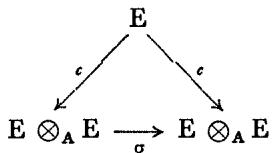
\includegraphics[keepaspectratio]{images/part004_07c99209.jpg}}

(其中 \(\sigma\) 是对称同态，使得 \(\sigma(x \otimes y) = y \otimes x\) ）是交换的（换句话说，只需余代数 E 与其反余代数（第1号，例2）相同即可）。

设 B 是交换 A-代数，u，v 是 C = Hom\_A(E, B) 的两个元素。

根据C中乘积的定义，uv和vu分别等于复合映射

\[
\mathrm{E} \xrightarrow {c} \mathrm{E} \otimes \mathrm{E} \xrightarrow {u \otimes v} \mathrm{B} \otimes \mathrm{B} \xrightarrow {m} \mathrm{B}
\]

和

\[
\mathrm{E} \xrightarrow {c} \mathrm{E} \otimes \mathrm{E} \xrightarrow {v \otimes u} \mathrm{B} \otimes \mathrm{B} \xrightarrow {m} \mathrm{B}.
\]

由此可知，若图(15)可交换，则代数 \(\operatorname{Hom}_{\mathbf{A}}(\mathbf{E}, \mathbf{B})\) 对每个可交换的A-代数B都是可交换的。为建立其逆命题，只需证明存在一个可交换的A-代数B以及两个A-线性映射 \(u, v\) 从 E 到 B 的映射，使得 \(m \circ (u \otimes v): \mathbf{E} \otimes \mathbf{E} \to \mathbf{B}\) 是单射。取 B 为代数 \(\mathsf{S}(\mathbf{E} \oplus \mathbf{E})\) ， \(u\) （相应地 \(v\) ）为典范映射 \(\mathbf{E} \oplus \mathbf{E} \to \mathsf{S}(\mathbf{E} \oplus \mathbf{E})\) 与映射 \(x \mapsto (x, 0)\) （相应地 \(x \mapsto (0, x)\) ）的复合，后者把 E 映入 \(\mathbf{E} \oplus \mathbf{E}\) 。若 \(h: \mathsf{S}(\mathbf{E}) \otimes \mathsf{S}(\mathbf{E}) \to \mathsf{S}(\mathbf{E} \otimes \mathbf{E})\) 是典范同构（ \(\S 6\) ，第6号，命题9）且 \(\lambda: \mathbf{E} \to \mathsf{S}(\mathbf{E})\) 是典范映射，那么 \(h^{-1} \circ m \circ (u \otimes v) = \lambda \otimes \lambda\) 。现在 \(\lambda \otimes \lambda\) 是单射的，因为 \(\lambda(\mathbf{E})\) 是 \(\mathsf{S}(\mathbf{E})\) 的直因子（II，§ 3，第7号，命题7的推论5）。

当余代数 E 满足命题2的条件时，称其为余交换的。

例子。（5）立即可以看出，余代数 A（第1号，例1）和余代数 \(\mathbf{A}^{(\mathbf{X})}\) （II，§ 11，第1号，例4）是余交换的。由第1号的公式（5）可知，余代数 S(M) 是余交换的。最后，对于 A-代数 B，使得 A-模 B 是投射的且有限生成的，要使余代数 \(\mathbf{B}^*\) （第1号，例3）是余交换的，其充分必要条件是 B 是交换的；因为（利用 A-模 B 与其双对偶的典范等同（II，§ 2，第7号）），这由图表（14）的交换性通过转置等价于表达 B 的交换性的图表（§ 1，第3号）这一事实得出。

命题3。设 E 是 A 上的一个余代数。为了使对于每个含单位元的 A-代数 B，A-代数 \(\operatorname{Hom}_{\mathbf{A}}(\mathbf{E},\mathbf{B})\) 是单位的，必要且充分条件是存在 E 上的一个线性形式 \(\gamma\) 使图表（16）交换

\begin{enumerate}
\def\labelenumi{(\arabic{enumi})}
\setcounter{enumi}{15}
\tightlist
\item
\end{enumerate}

\pandocbounded{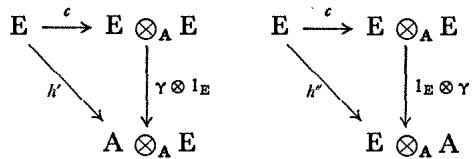
\includegraphics[keepaspectratio]{images/part004_cc0e83d1.jpg}}

（其中 \(c: \mathbf{E} \to \mathbf{E} \otimes_{\mathbf{A}} \mathbf{E}\) 是余积，并且 \(h'\) 和 \(h''\) 是典范同构（II，§ 3，第4号，命题4）。 \(\operatorname{Hom}_{\mathbf{A}}(\mathbf{E}, \mathbf{B})\) 的单位元则是线性映射 \(x \mapsto \gamma(x)1\) （其中1表示B的单位元）。

设 \(\gamma\) 是 E 上的一个线性形式，使得图表（16）交换。设 B 是带单位元 1 的含单位元 A-代数， \(\eta: \mathbf{A} \to \mathbf{B}\) 为典范映射， \(v = \eta \circ \gamma\) 为 A-代数 \(\mathbf{C} = \operatorname{Hom}_{\mathbf{A}}(\mathbf{E}, \mathbf{B})\) 的元素。对于每个元素 \(u \in \mathbf{C}\) ， \(uv\) 是复合映射

\[
\mathrm{E} \xrightarrow {c} \mathrm{E} \otimes \mathrm{E} \xrightarrow {1 _ {\mathrm{E}} \otimes \gamma} \mathrm{E} \otimes \mathrm{A} \xrightarrow {u \otimes \eta} \mathrm{B} \otimes \mathrm{B} \xrightarrow {m} \mathrm{B}.\tag{17}
\]

那么 \(uv = m \circ (u \otimes \eta) \circ h'' = u\) 。类似地可证明 \(vu = u\) ，因此 \(v\) 是 C 的单位元。反之，设 A-模 A ⊕ E 被赋予一个含单位元的代数结构，使得 \((a, x)(a', x') = (aa', ax' + a'x)\) （对 A 中的 \(a, a'\) 和 E 中的 \(x, x'\) ）。设 B 表示如此定义的 A-代数，并设 C 为 A-代数 Hom \(_A(E, B)\) 。假设 C 是含单位元的，并设 \(e: x \mapsto (\gamma(x), \lambda(x))\) 为其单位元（其中 \(\gamma(x) \in A\) 和 \(\lambda(x) \in E\) ）。另一方面，设 \(f\) 是 C 的元素 \(x \mapsto (0, x)\) 。直接计算表明 \(fe\) 是元素

\[
x \mapsto (0, (h ^ {\prime \prime}) ^ {- 1} ((1 _ {E} \otimes \gamma) (c (x))))
\]

此元素属于 C 。条件 \(fe = f\) 蕴含 (16) 中第二个图的交换性，并且类似地可看出条件 \(ef = f\) 蕴含 (16) 中第一个图的交换性。

E 上使图 (16) 交换的线性形式 \(\gamma\) 称为余代数 E 的余单位。一个余代数至多有一个余单位：因为它就是代数 \(\operatorname{Hom}_{\mathbf{A}}(\mathbf{E}, \mathbf{A})\) 的单位元。带有余单位的余代数称为余单位的。

例子。(6) 恒等映射是余代数 A 的余单位；在余代数 \(\mathbf{A}^{(\mathbf{X})}\) （第 1 号，例 4）上，线性形式 \(\gamma\) （使得 \(\gamma(e_x) = 1\) 对所有 \(x \in \mathbf{X}\) 成立）是余单位。在余代数 \(\mathbf{T}(\mathbf{M})\) （相应地 \(\mathbf{S}(\mathbf{M}), \bigwedge(\mathbf{M})\) ）上，线性形式 \(\gamma\) （满足 \(\gamma(1) = 1\) 且 \(\gamma(z) = 0\) ，其中 \(z\) 属于 \(\mathbf{T}^n(\mathbf{M})\) （相应地 \(\mathbf{S}^n(\mathbf{M}), \bigwedge^n(\mathbf{M})\) ）， \(n \geqslant 1\) ）是余单位。最后，设 B 是一个 A-代数，它是有限生成的投射 A-模，并且有单位元 \(e\) ；则在余代数 \(\mathbf{B}^*\) （第1号，例3）上，线性形式 \(\gamma: x^* \mapsto \langle e, x^* \rangle\) 是余单位，因为这个形式恰好是从 A 到 B 的 A-线性映射 \(\eta_e: \xi \mapsto \xi e\) 的转置，并且通过转置，图（16）的交换性可由那些表达（利用 \(\eta_e\) ）"\(e\) 是 B 的单位元"这一事实的图的交换性推出（ \(\S 1\) ，第 3 号）；同样的论证还表明，反之，若余代数 \(\mathbf{B}^*\) 具有一个余单位 \(\gamma\) ，则 \(\gamma\) 的转置定义 B 的单位元 \(e = {}^t\gamma(1)\) 。

命题 4. 设 E 是一个具有余单位 \(\gamma\) 的余代数，并假设 E 中存在一个元素 \(e\) ，使得 \(\gamma(e) = 1\) ；则 E 是子 A-模 Ae 与 \(\mathrm{E}_{\gamma} = \mathrm{Ker}(\gamma)\) 的直和，且

\[
c (e) \equiv e \otimes e (\mathrm{mod.} \mathrm{E} _ {\gamma} \otimes \mathrm{E} _ {\gamma})\tag{18}
\]

\[
\left\{c (x) \equiv x \otimes e + e \otimes x (\mathrm{mod.} \mathrm{E} _ {\gamma} \otimes \mathrm{E} _ {\gamma}) \quad \text { for all } x \in \mathrm{E} _ {\gamma}. \right.
\]

第一个断言是直接的，因为 \(\gamma(x - \gamma(x)e) = 0\) 以及关系 \(\gamma(\alpha e) = 0\) 蕴含 \(\alpha = 0\) 。设 \(c(e) = \sum_{i} s_i \otimes t_i\) ，使得

\[
e = \sum_ {i} \gamma (s _ {i}) t _ {i} = \sum_ {i} \gamma (t _ {i}) s _ {i}
\]

由 (16) 及 \(1 = \gamma(e) = \sum_{i} \gamma(s_i) \gamma(t_i)\) 得出。因此

\[
\begin{array}{r l} \sum_ {i} (s _ {i} - \gamma (s _ {i}) e) \otimes (t _ {i} - \gamma (t _ {i}) e) & = \sum_ {i} s _ {i} \otimes t _ {i} - \sum_ {i} e \otimes \gamma (s _ {i}) t _ {i} \\ & - \sum_ {i} \gamma (t _ {i}) s _ {i} \otimes e \\ & + \sum_ {i} \gamma (s _ {i}) e \otimes \gamma (t _ {i}) e \end{array}
\]

而根据上述关系，这正好是 \(c(e) - e \otimes e\) ；因此这证明了 (18) 中的第一个关系。另一方面，E \(\otimes\) E 作为直和的分解

\[
\mathbf {A} (e \otimes e) \oplus ((\mathbf {A} e) \otimes \mathbf {E} _ {\gamma}) \oplus (\mathbf {E} _ {\gamma} \otimes (\mathbf {A} e)) \oplus (\mathbf {E} _ {\gamma} \otimes \mathbf {E} _ {\gamma})
\]

使得我们可以写出，对于 \(x \in \mathbf{E}_{\gamma}\) , \(c(x) = \lambda(e \otimes e) + (e \otimes y) + (z \otimes e) + u\) （其中 \(u = \sum_{j} v_{j} \otimes w_{j}, y, z\) ，而 \(v_{j}\) 和 \(w_{j}\) 属于 \(\mathbf{E}_{\gamma}\) ）。余单位 \(\gamma\) 的定义随后给出 \(x = \lambda e + y = \lambda e + z\) ，并且由于 \(\gamma(x) = 0\) ，必然有 \(\lambda = 0, x = y = z\) ，由此得出 (18) 的第二个关系式。

注记。设 C 是一个有余单位的余结合 A-余代数，B 是一个含单位元的结合 A-代数，M 是一个左 B-模。A-双线性映射 \((b, m) \mapsto bm\) （从 \(B \times M\) 到 M 中）定义了一个 A-双线性映射

\[
\operatorname{Hom} _ {\mathbf {A}} (\mathrm{C}, \mathrm{B}) \times \operatorname{Hom} _ {\mathbf {A}} (\mathrm{C}, \mathrm{M}) \rightarrow \operatorname{Hom} _ {\mathbf {A}} (\mathrm{C}, \mathrm{M})
\]

这通过本号开头所述的一般程序完成。可以立即验证，该映射在 \(\operatorname{Hom}_{\mathbf{A}}(\mathbf{C}, \mathbf{M})\) 上定义了环 \(\operatorname{Hom}_{\mathbf{A}}(\mathbf{C}, \mathbf{B})\) 上的一个左模结构。

\subsection{N型分次余代数的性质}

命题5. (i) 设 E 是一个具有余单位 \(\gamma\) 的分次余代数；则 \(\gamma\) 是次数为 0 的齐次线性形式。

\begin{enumerate}
\def\labelenumi{(\roman{enumi})}
\setcounter{enumi}{1}
\tightlist
\item
  进一步假设存在一个元素 \(e \in \mathbf{E}\) ，使得 \(\mathbf{E}_0 = \mathbf{A}e\) 且 \(\gamma(e) = 1\) 。那么 \(\mathbf{E}_{\gamma}\) （即 \(\gamma\) 的核）等于 \(\mathbf{E}_{+} = \sum_{n \geqslant 1} \mathbf{E}_n, c(e) = e \otimes e\) 和
\end{enumerate}

\[
c (x) \equiv x \otimes e + e \otimes x (\mathrm{mod.} \mathrm{E} _ {+} \otimes \mathrm{E} _ {+})\tag{19}
\]

对所有 \(x \in \mathbf{E}_{+}\) 。

\begin{enumerate}
\def\labelenumi{(\roman{enumi})}
\tightlist
\item
  只需验证 \(\gamma(x) = 0\) （对 \(x \in \mathbf{E}_n\) ，对所有 \(n \geqslant 1\) ）。由于 \(c\) 是次数为 0 的分次同态，
\end{enumerate}

\[
c (x) = \sum_ {0 \leqslant j \leqslant n} \left(\sum_ {i} y _ {i j} \otimes z _ {i, n - j}\right)\tag{20}
\]

其中，对所有 \(j\) （满足 \(0 \leqslant j \leqslant n\) ）， \(y_{ij}\) 和 \(z_{ij}\) 在 \(\mathbf{E}_j\) 中；应用（16）（第2号），我们得到

\[
x = \sum_ {0 \leqslant j \leqslant n} \left(\sum_ {i} \gamma (y _ {i j}) z _ {i, n - j}\right) = \sum_ {0 \leqslant j \leqslant n} \left(\sum_ {i} \gamma (z _ {i, n - j}) y _ {i j}\right),
\]

因此，比较两边次数为0和次数为n的分量，可得

\[
x = \sum_ {i} \gamma (y _ {i 0}) z _ {i n} = \sum_ {i} \gamma (z _ {i 0}) y _ {i n}
\]

\[
0 = \sum_ {i} \gamma (y _ {i n}) z _ {i 0} = \sum_ {i} \gamma (z _ {i n}) y _ {i 0}
\]

从而 \(\gamma(x) = \sum_{i} \gamma(y_{in})\gamma(z_{i0}) = \gamma(0) = 0\) 。

\begin{enumerate}
\def\labelenumi{(\roman{enumi})}
\setcounter{enumi}{1}
\tightlist
\item
  由于 \(\operatorname{Ker}(\gamma)\) 和 \(\mathbf{E}_{+}\) 都是 \(Ae = E_0\) 的补子模，且由（i）有 \(\mathbf{E}_{+} \subset \operatorname{Ker}(\gamma)\) ，故 \(\mathbf{E}_{+} = \operatorname{Ker}(\gamma)\) (II，§1，第8号，注记1)；其余断言由第2号命题4推出。
\end{enumerate}

命题6. 设E为A上的分次余代数。为使对每个交换A-代数B（具有平凡分次），型为Z的分次A-代数Homgr \(_{A}\) (E, B)（第2号）是反交换的（§4，第9号，定义7），其充分必要条件为，若 \(\sigma_{g}\) 表示 A-模 E \(\otimes_{A} E\) 的自同构，使得

\[
\sigma_ {g} (x _ {p} \otimes x _ {q}) = (- 1) ^ {p q} x _ {q} \otimes x _ {p}
\]

对 \(x_{p} \in \mathbf{E}_{p}, x_{q} \in \mathbf{E}_{q}\) （其中 \(p\) 和 \(q\) 是 \(\mathbf{N}\) 中的任意元素），该图表

\begin{enumerate}
\def\labelenumi{(\arabic{enumi})}
\setcounter{enumi}{20}
\tightlist
\item
\end{enumerate}

\pandocbounded{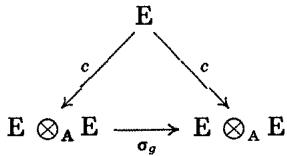
\includegraphics[keepaspectratio]{images/part004_b841500b.jpg}}

是交换的。

证明与第2号的命题2的证明类似。

当分次余代数 E 满足命题6的条件时，称其为余反交换的。

例。由第1号公式 (8) 直接可得，对每个 A-模 M，分次余代数 \(\bigwedge(M)\) 是余反交换的。

\subsection{双代数与斜双代数}

定义3. 环A上的分次双代数（相应地，斜分次双代数）是一个集合E，它带有N型的分次A-代数结构和N型的分次A-余代数结构，且两者具有相同的底层分次A-模结构，并满足：

\begin{enumerate}
\def\labelenumi{(\arabic{enumi})}
\item
  A-代数 E 是结合的且有单位元的。
\item
  A-余代数 E 是余结合的且有余单位。
\item
  余积 \(c: \mathbf{E} \to \mathbf{E} \otimes_{\mathbf{A}} \mathbf{E}\) 是从分次代数 \(\mathbf{E}\) 到分次代数 \(\mathbf{E} \otimes_{\mathbf{A}} \mathbf{E}\) （相应地，分次代数 \(\mathbf{E}^{\mathfrak{g}} \otimes_{\mathbf{A}} \mathbf{E}\) ，参见§4，第7号）中的同态。
\item
  余单位 \(\gamma\) （E 的）是从分次代数 E 到代数 A（带平凡分次）中的分次代数同态，使得若 e 表示 A-代数 \(\mathbf{E}, \gamma(e) = 1\) 。
\end{enumerate}

如果 E 是一个分次双代数且其分次是平凡的，则 E 简称为双代数。一个分次双代数称为交换的（相应地，余交换的），如果其底代数是交换的（相应地，如果其底余代数是余交换的）；一个斜分次双代数称为反交换的（相应地，余反交换的），如果其底分次代数是反交换的（相应地，如果其底分次余代数是余反交换的）。

由定义3及第2节命题5可知，对于分次双代数或斜分次双代数E，

\[
\left\{ \begin{array}{c} c (e) = e \otimes e \\ c (x) \equiv x \otimes e + e \otimes x (\mathrm{mod.} \mathrm{E} _ {+} \otimes \mathrm{E} _ {+}) \quad \text { for } x \in \mathrm{E} _ {+} = \bigoplus_ {n \geqslant 1} \mathrm{E} _ {n}. \end{array} \right.\tag{22}
\]

若E和F是两个分次双代数（相应地，两个斜分次双代数），则一个映射 \(\phi: \mathrm{E} \to \mathrm{F}\) 称为分次双代数态射（相应地，斜分次双代数态射），如果：（1） \(\phi\) 是一个分次代数态射（因此将E的单位元映到F的单位元）；（2） \(\phi\) 是一个分次余代数态射，使得若 \(\gamma\) 和 \(\gamma'\) 分别是E和F的余单位，则 \(\gamma = \gamma' \circ \phi\) .

例子。（1）设 S 是一个具有单位元 u 的幺半群，于是幺半群 S 在 A 上的代数 \(E = A^{(S)}\) 具有单位元 \(e_{u}\) (§2，第6号)；另一方面已经看到，E 典范地具有一个带余单位 \(\gamma\) 的余结合、余交换 A-余代数结构，使得 \(\gamma(e_{s}) = 1\) （对所有 \(s \in S\) ）（第1号，例4及第2号，例4、例5和例6）。给出余积的公式 \(c(e_{s}) = e_{s} \otimes e_{s}\) 也立即表明 c 是一个代数同态。因此在 E 上定义了一个余交换双代数结构，带此结构的 E 被称为幺半群 S 在 A 上的双代数。

如果 T 是另一个带有单位元的幺半群， \(v, f: \mathrm{S} \to \mathrm{T}\) 为一个同态，使得 \(f(u) = v\) ，而 \(f_{(\mathbf{A})}: \mathrm{A}^{(\mathrm{S})} \to \mathrm{A}^{(\mathrm{T})}\) 为由 \(f(\S 2, \text{no. } 6)\) 导出的 A-代数同态，则可立即验证 \(f_{(\mathbf{A})}\) 是一个双代数同态。

\begin{enumerate}
\def\labelenumi{(\arabic{enumi})}
\setcounter{enumi}{1}
\item
  设 M 为一个 A-模。在 S(M) 上定义的分次 A-代数（§ 6，第 1 号）和分次 A-余代数（第 1 号，例 6）结构，在此集合上定义了一个交换余交换的分次双代数结构；因为我们已经看到（第 1 号，例 6），S(M) 上的余积是一个代数同态，并且由余单位 \(\gamma\) 的定义（第2号，例6）可知 \(\gamma(1) = 1\) ，且 \(\gamma\) 是从 \(E\) 到 \(A\) 中的代数同态。
\item
  设 M 为 A-模。我们如同例 2 中那样看到， \(\bigwedge\) (M) 上的分次 A-代数（§ 7，第 1 号）和分次 A-余代数（第 1 号，例 7）结构在此集合上定义一个反交换、余反交换的斜分次双代数结构。
\end{enumerate}

注：若 M 是一个 A-模，使得 \(M \otimes_{A} M \neq \{0\}\) ，则分次 A-代数（§ 5，第 1 号）和分次 A-余代数（第 1 号，例 5）在 T(M) 上的结构并不定义一个双代数结构，因为一般地

\[
c (x _ {1} x _ {2} y _ {1} y _ {2}) \neq c (x _ {1} x _ {2}) c (y _ {1} y _ {2})
\]

对 M 的四个元素 \(x_{1}, x_{2}, y_{1}, y_{2}\) 成立，如第1号公式 (3) 所示。

\subsection{分次对偶 T(M)*gr、S(M)*gr 与 ∧(M)*gr}

从现在起，我们回到关于代数的章节的一般约定，因此（除非另有说明）假定这些代数是结合的且有单位的。

设 M 为一个 A-模；定义在 T(M)（第 1 号，例 5）、S(M)（第 1 号，例 6）和 \(\bigwedge\) (M)（第1号，例7）上的分次 A-余代数结构，依据第 2 号的命题 1 和命题 3 以及关于分次模的分次对偶的分次所作的约定（第 1 号），使我们能够典范地在分次对偶 T(M)*gr、S(M)*gr 和 \(\bigwedge\) (M)*gr 上定义 N 型分次代数结构。此外，分次代数 S(M)*gr 是交换的（第 2 号，命题 2 和例 5），且分次代数 \(\bigwedge\) (M)*gr 是反交换的（第3号，命题6及例）。在 \(\bigwedge\) (M)*gr 中，每个次数为 1 的元素的平方为零；这样的元素等同于 M 上的一个线性形式 \(f\) ，其平方是交错双线性形式 \(f \wedge f\) （在 M \(^{2}\) 上），使得

\[
(f \wedge f) (x, y) = f (x) f (y) - f (y) f (x)
\]

（第 2 号，例 3）。

设 \(\mathbf{N}\) 是另一个 A-模，且 \(u\) 为从 \(\mathbf{M}\) 到 \(\mathbf{N}\) 中的一个 A-线性映射。我们知道 \(u\) 典范地定义分次代数同态

\[
\left\{ \begin{array}{l} \mathsf {T} (u): \mathsf {T} (\mathbf {M}) \to \mathsf {T} (\mathbf {N}) \\ \mathsf {S} (u): \mathsf {S} (\mathbf {M}) \to \mathsf {S} (\mathbf {N}) \\ \bigwedge (u): \bigwedge (\mathbf {M}) \to \bigwedge (\mathbf {N}) \end{array} \right.\tag{23}
\]

（§ 5，第 2 号，§ 6，第 2 号和 § 7，第 2 号）。由第 1 号的公式 (3) 可立即验证 \(\mathsf{T}(u)\) 也是余代数态射。另一方面，若 \(\Delta_{\mathbf{M}}\) （相应地 \(\Delta_{\mathbf{N}}\) ）

表示对角映射 \(\mathbf{M} \to \mathbf{M} \times \mathbf{M}\) （相应地 \(\mathbf{N} \to \mathbf{N} \times \mathbf{N}\) ），则有关系式 \((u \times u) \circ \Delta_{\mathbf{M}} = \Delta_{\mathbf{N}} \circ u\) ；由此可得 \(\mathbf{S}(u \times u) \circ \mathbf{S}(\Delta_{\mathbf{M}}) = \mathbf{S}(\Delta_{\mathbf{N}}) \circ \mathbf{S}(u)\)

\[
(\text { resp. } \bigwedge (u \times u) \circ \bigwedge (\Delta_ {\mathbf {M}}) = \bigwedge (\Delta_ {\mathbf {N}}) \circ \bigwedge (u)).
\]

利用 \(\mathsf{S}(\mathbf{M})\) 和 \(\bigwedge (\mathbf{M})\) 中余积的定义（第 1 号，例 6 和 7）以及典范同构的函子性质，

\[
\mathbf {S} (\mathbf {M} \times \mathbf {M}) \rightarrow \mathbf {S} (\mathbf {M}) \otimes_ {\mathbf {A}} \mathbf {S} (\mathbf {M})
\]

和 \(\bigwedge (\mathbf{M}\times \mathbf{M})\to \bigwedge (\mathbf{M})^{\mathfrak{g}}\otimes_{\mathbf{A}}\bigwedge (\mathbf{M})\) ，可以看出 \(S(u)\) 和 \(\bigwedge (u)\) 也是余代数态射†（因此在这种情况下是双代数态射）。由此立即得出同态 (23) 的分次转置（II，§ 11，第 6 号）

\[
\begin{array}{c} ^ {t} \mathsf {T} (u): \mathsf {T} (\mathbf {N}) ^ {* \mathrm{gr}} \to \mathsf {T} (\mathbf {M}) ^ {* \mathrm{gr}} \\ ^ {t} \mathsf {S} (u): \mathsf {S} (\mathbf {N}) ^ {* \mathrm{gr}} \to \mathsf {S} (\mathbf {M}) ^ {* \mathrm{gr}} \\ ^ {t} \bigwedge (u): \bigwedge (\mathbf {N}) ^ {* \mathrm{gr}} \to \bigwedge (\mathbf {M}) ^ {* \mathrm{gr}} \end{array}
\]

是分次代数同态。

我们现在注意到，M 的对偶 M* 与 T(M)*gr（相应地，S(M)*gr，∧(M)*gr）中次数为 1 的元素所构成的子模等同。因此，由张量代数的泛性质（§ 5，第 1 号）和对称代数的泛性质（§ 6，第 1 号）可知，存在且仅存在一个分次代数同态

\[
\theta_ {\mathsf {T}}: T (M ^ {*}) \rightarrow T (M) ^ {* \mathrm{gr}}
\]

它延拓了典范单射 \(\mathbf{M}^{*}\to \mathsf{T}(\mathbf{M})^{*\mathrm{gr}}\) ，并且存在唯一一个分次代数同态

\[
\theta_ {\mathsf {S}}: S (M ^ {*}) \rightarrow S (M) ^ {* \mathrm{gr}}
\]

它延拓了典范单射 \(\mathbf{M}^{*}\to\mathsf{S}(\mathbf{M})^{*\mathrm{gr}}\) 。另一方面， \(\mathbf{M}^{*}\) 在 \(\bigwedge(\mathbf{M})^{*\mathrm{gr}}\) 的反代数中的典范单射使得 \(\mathbf{M}^{*}\) 的每个元素的平方为零；因此（§ 7，第 1 号，命题 1）存在唯一一个分次代数同态

\[
\theta_ {\wedge}: \bigwedge (\mathbf {M} ^ {*}) \rightarrow (\bigwedge (\mathbf {M}) ^ {* \mathrm{gr}}) ^ {\circ}
\]

它延拓了典范单射 \(M^{*}\to\bigwedge(M)^{*gr.}\) 。这些同态是函子性的：例如，对于每个 A-模同态 \(u:M\to N\) ，该图表

\pandocbounded{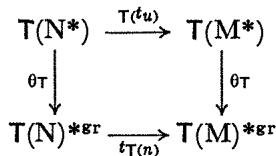
\includegraphics[keepaspectratio]{images/part004_1f4c9f33.jpg}}

是交换的，这直接从张量代数的泛性质（§ 5，第 1 号）得出；对 \(\theta_{s}\) 和 \(\theta_{\wedge}\) 也有类似的交换图。

我们将明确找出同态 \(\theta_{\mathsf{T}}\) , \(\theta_{\mathsf{S}}\) 和 \(\theta_{\wedge}\) 。为此，我们更一般地考虑一个带余积 \(c\) 的余结合 A-余代数 E，并对 \(n\) （ \(n \geqslant 2\) ）归纳地定义线性映射 \(c_{n}\) （从 E 到 \(\mathrm{E}^{\otimes n}\) 中），由 \(c_{2} = c\) 和

\[
c _ {n} = \left(c _ {n - 1} \otimes 1 _ {\mathrm{E}}\right) \circ c.\tag{24}
\]

另一方面，我们用 \(m_{n}:A^{\otimes n}\to A\) 表示典范线性映射，使得 \(m_{n}(\xi_{1}\otimes\xi_{2}\otimes\cdots\otimes\xi_{n})=\xi_{1}\xi_{2}\ldots\xi_{n}\) ，并注意，对 \(n\geqslant2\) ，

\[
m _ {n} = m \circ (m _ {n - 1} \otimes 1 _ {\mathbf {A}})\tag{25}
\]

记 \(m = m_2\) 。利用此记号：

引理1. (i) 在结合代数 \(\mathbf{E}^* = \operatorname{Hom}_{\mathbf{A}}(\mathbf{E}, \mathbf{A})\) 中， \(n\) 个 1 次元素 \(u_1, u_2, \ldots, u_n\) 的乘积由

\[
u _ {1} u _ {2} \dots u _ {n} = m _ {n} \circ (u _ {1} \otimes u _ {2} \otimes \dots \otimes u _ {n}) \circ c _ {n}.\tag{26}
\]

\begin{enumerate}
\def\labelenumi{(\roman{enumi})}
\setcounter{enumi}{1}
\tightlist
\item
  还假设余代数 E 是分次的。那么，在分次结合代数 \(\mathbf{E}^{*\mathrm{gr}} = \operatorname{Homgr}_{\mathbf{A}}(\mathbf{E}, \mathbf{A})\) 中， \(n\) 个 1 次元素 \(u_1, u_2, \ldots, u_n\) 的乘积由
\end{enumerate}

\[
u _ {1} u _ {2} \dots u _ {n} = m _ {n} \circ (u _ {1} \otimes u _ {2} \otimes \dots \otimes u _ {n}) \circ \delta_ {n}\tag{27}
\]

（其中 \(\delta_n: \mathbf{E} \to \mathbf{E}^{\otimes n}\) 是把每个 \(x \in \mathbf{E}\) 映为 \(c_n(x)\) 的多重次数 \((1, 1, \ldots, 1)\) 分量的线性映射。

公式（26）正是 \(\mathbf{E}^*\) 中乘积在 \(n = 2\) 时的定义；要对 \(n\) 用归纳法证明它，观察到

\[
\begin{array}{l} u _ {1} u _ {2} \dots u _ {n} \\ \qquad = m \circ ((u _ {1} u _ {2} \dots u _ {n - 1}) \otimes u _ {n}) \circ c \\ \qquad = m \circ ((m _ {n - 1} \circ (u _ {1} \otimes u _ {2} \otimes \dots \otimes u _ {n - 1}) \circ c _ {n - 1}) \otimes u _ {n}) \circ c \\ \qquad = m \circ (m _ {n - 1} \otimes \mathrm{l} _ {\mathrm{A}}) \circ (u _ {1} \otimes u _ {2} \otimes \dots \otimes u _ {n - 1} \otimes u _ {n}) \circ (c _ {n - 1} \otimes \mathrm{l} _ {\mathrm{E}}) \circ c \\ \qquad = m _ {n} \circ (u _ {1} \otimes u _ {2} \otimes \dots \otimes u _ {n}) \circ c _ {n} \end{array}
\]

根据（24）、（25）、II，§3，第3号，公式（5）以及关系式

\[
u _ {n} = 1 _ {\mathbf {A}} \circ u _ {n} \circ 1 _ {\mathbf {E}}.
\]

当 E 是分次的且元素 \(u_{i} \in E^{*gr}\) 是 1 次齐次的时，根据定义，对齐次元素 \(x_{i} \in E\) ，

\[
(u _ {1} \otimes u _ {2} \otimes \dots \otimes u _ {n}) (x _ {1} \otimes x _ {2} \otimes \dots \otimes x _ {n}) = 0
\]

除非所有 \(x_{i}\) 的次数均为 1，由此得到公式 (27) 。

由第1号中的公式 (3)、(5)和(7)以及公式 (24) 可知，当 E 取为三个分次余代数 \(\mathsf{T}(\mathbf{M})\) , \(\mathsf{S}(\mathbf{M})\) 和 \(\bigwedge (\mathbf{M})\) 之一时，对 \(n\) 用归纳法（利用余积是次数为 0 的分次同态这一事实）分别得到，对 M 中的 \(x_{1}, x_{2}, \ldots, x_{n}\) ：

\[
\text { when   } \mathrm{E} = \mathrm{T} (\mathrm{M}), \quad \delta_ {n} (x _ {1} x _ {2} \dots x _ {n}) = x _ {1} \otimes x _ {2} \otimes \dots \otimes x _ {n}
\]

\[
\text { when } \mathrm{E} = \mathrm{S(M)}, \quad \delta_ {n} (x _ {1} x _ {2} \dots x _ {n}) = \sum_ {\sigma \in \mathfrak {S} _ {n}} x _ {\sigma (1)} \otimes x _ {\sigma (2)} \otimes \dots \otimes x _ {\sigma (n)}
\]

\[
\text { when } \mathrm{E} = \bigwedge (\mathrm{M}), \quad \delta_ {n} (x _ {1} x _ {2} \dots x _ {n}) = \sum_ {\sigma \in \mathfrak {S} _ {n}} \varepsilon_ {\sigma}. x _ {\sigma (1)} \otimes x _ {\sigma (2)} \otimes \dots \otimes x _ {\sigma (n)}.
\]

只需注意，例如当 \(\mathbf{E} = \bigwedge (\mathbf{M})\) 时，在由第1号公式 (8) 得出的表达式 \(c_{n}(x_{1}x_{2}\ldots x_{n}) = (c_{n - 1}\otimes 1_{\mathbb{E}})\left(\sum (-1)^{\nu}(x_{i_1}\ldots x_{i_p})\otimes (x_{j_1}\ldots x_{j_{n - p}})\right)\) 中，唯一能给出多重次数 \((1,1,\dots ,1)\) 项的是那些使 \(n - p = 1\) 的项，因此

\[
\delta_ {n} (x _ {1} x _ {2} \dots x _ {n})
\]

是以下和中多重次数为 \((1, 1, \ldots, 1)\) 的项

\[
\sum_ {i = 1} ^ {n} (- 1) ^ {n - i} c _ {n - 1} \left(x _ {1} \dots x _ {i - 1} x _ {i + 1} \dots x _ {n}\right) \otimes x _ {i}
\]

且这一项必然等于

\[
\sum_ {i = 1} ^ {n} (- 1) ^ {n - i} \delta_ {n - 1} (x _ {1} \dots x _ {i - 1} x _ {i + 1} \dots x _ {n}) \otimes x _ {i},
\]

因此由归纳假设可得结果。

根据引理1， \(\mathsf{T}(\mathbf{M})^{*\mathrm{gr}}\) 中 \(n\) 个线性形式 \(x_{1}^{*}, x_{2}^{*}, \ldots, x_{n}^{*}\) （属于 \(\mathbf{M}^{*}\) ）的乘积由以下公式给出

\[
\left\langle x _ {1} ^ {*} x _ {2} ^ {*} \dots x _ {n} ^ {*}, x _ {1} x _ {2} \dots x _ {n} \right\rangle = \prod_ {i = 1} ^ {n} \left\langle x _ {i} ^ {*}, x _ {i} \right\rangle\tag{28}
\]

对 \(x_{i} \in \mathbf{M} (1 \leqslant i \leqslant n)\) 成立；这 \(n\) 个形式在 \(S(M)^{*gr}\) 中的乘积由以下公式给出

\[
\left\langle x _ {1} ^ {*} x _ {2} ^ {*} \dots x _ {n} ^ {*}, x _ {1} x _ {2} \dots x _ {n} \right\rangle = \sum_ {\sigma \in \mathfrak {S} _ {n}} \left(\prod_ {i = 1} ^ {n} \left\langle x _ {\sigma (i)} ^ {*}, x _ {i} \right\rangle\right);\tag{29}
\]

最后，这些形式在 \(\bigwedge (\mathbf{M})^{*\mathrm{gr}}\) 中的乘积由以下公式给出

\[
\langle x _ {1} ^ {*} x _ {2} ^ {*} \dots x _ {n} ^ {*}, x _ {1} x _ {2} \dots x _ {n} \rangle = \det (\langle x _ {i} ^ {*}, x _ {j} \rangle).\tag{30}
\]

在三种情形中，我们分别有

\[
\theta_ {T} (x _ {1} ^ {*} \otimes x _ {2} ^ {*} \otimes \dots \otimes x _ {n} ^ {*}) = x _ {1} ^ {*} x _ {2} ^ {*} \dots x _ {n} ^ {*}
\]

\[
\theta_ {S} (x _ {1} ^ {*} x _ {2} ^ {*} \dots x _ {n} ^ {*}) = x _ {1} ^ {*} x _ {2} ^ {*} \dots x _ {n} ^ {*}
\]

\[
\theta_ {\wedge} (x _ {1} ^ {*} \wedge x _ {2} ^ {*} \wedge \dots \wedge x _ {n} ^ {*}) = x _ {n} ^ {*} x _ {n - 1} ^ {*} \dots x _ {1} ^ {*} = (- 1) ^ {n (n - 1) / 2} x _ {1} ^ {*} x _ {2} ^ {*} \dots x _ {n} ^ {*}
\]

因此，我们从 (28)、(29) 和 (30) 推导出以下关系式

\[
\langle \theta_ {T} (x _ {1} ^ {*} \otimes x _ {2} ^ {*} \otimes \dots \otimes x _ {n} ^ {*}), x _ {1} \otimes x _ {2} \otimes \dots \otimes x _ {n} \rangle = \prod_ {i = 1} ^ {n} \langle x _ {i} ^ {*}, x _ {i} \rangle\tag{28 bis}
\]

（换言之， \(\theta_{\mathsf{T}}\) 在 \(\mathsf{T}^2 (\mathbf{M}^*)\) 上的限制就是 II，§4，第4号中的典范同态）

\[
\langle \theta_ {\mathsf {S}} (x _ {1} ^ {*} x _ {2} ^ {*} \dots x _ {n} ^ {*}), x _ {1} x _ {2} \dots x _ {n} \rangle = \sum_ {\sigma \in \mathfrak {S} _ {n}} \left(\prod_ {i = 1} ^ {n} \langle x _ {\sigma (i)} ^ {*}, x _ {i} \rangle\right)\tag{29 bis}
\]

\[
\begin{array}{r l} (30 \text { bis}) &\langle \theta_ {\wedge} (x _ {1} ^ {*} \wedge x _ {2} ^ {*} \wedge \dots \wedge x _ {n} ^ {*}), x _ {1} \wedge x _ {2} \wedge \dots \wedge x _ {n} \rangle \\ & \qquad = (- 1) ^ {n (n - 1) / 2} \mathrm{det} (\langle x _ {i} ^ {*}, x _ {j} \rangle). \end{array}
\]

命题7. 设 \(\mathbf{M}\) 是有限生成的投射 A-模。则典范同态 \(\theta_{\mathsf{T}}: \mathsf{T}(\mathbf{M}^{*}) \to \mathsf{T}(\mathbf{M})^{*\mathrm{gr}}\) 和 \(\theta_{\wedge}: \bigwedge (\mathbf{M}^{*}) \to (\bigwedge (\mathbf{M})^{*\mathrm{gr}})^{0}\) 是双射。此外，分次对偶 \(\bigwedge (\mathbf{M})^{*\mathrm{gr}}\) 此时等于对偶 \(\bigwedge (\mathbf{M})^{*}\) ，即 A-模 \(\bigwedge (\mathbf{M})\) 的对偶。

首先假设 \(\mathbf{M}\) 具有有限基 \((e_i)_{1\leq i\leq m}\) ，并设 \((e_i^*)_{1\leq i\leq m}\) 为 \(\mathbf{M}^*\) 的对偶基 (II, § 10, no. 4)。公式 (28 bis) 表明，对每个有限序列 \(s = (j_k)_{1\leq k\leq n}\) （ \(n\) 个元素取自区间 \([1,m]\) （ \(\mathbf{N}\) 的）），

\[
\theta_ {\mathsf {T}} (e _ {j _ {1}} ^ {*} \otimes \dots \otimes e _ {j _ {n}} ^ {*})
\]

是指标为 \(s\) 的元素，位于 \((\mathsf{T}^n (\mathbf{M}))^*\) 的基中，该基对偶于 \(\mathsf{T}^n (\mathbf{M})\) 的由 \(e_s = e_{j_1}\otimes \dots \otimes e_{j_n}\) 组成的基（§ 5，第 5 号，定理 1）。因此 \(\theta_{\mathsf{T}}\) 是双射。

类似地，公式（30 bis）表明，对每个有限子集 \(\mathbf{H}\) （属于 \([1, m]\) ，含 \(n\) 个元素）， \((-1)^{n(n-1)/2} \theta_{\wedge}(e_{\mathrm{H}}^{*})\) （§7，第8号，定理1的记号）是指标为 \(\mathbf{H}\) 的元素，位于 \((\bigwedge^{n}(\mathbf{M}))^{*}\) 的基中，该基对偶于 \(\bigwedge^{n}(\mathbf{M})\) 的由 \(e_{\mathrm{H}}\) 组成的基。因此 \(\theta_{\wedge}\) 是双射。

现在仅假设 M 是有限生成且投射的；则 M 是有限生成自由 A-模 L 的一个直和因子，因此存在两个

A-线性映射 \(M \xrightarrow{j} L \xrightarrow{p} M\) ，其复合为恒等映射 \(1_{M}\) 。由此我们推导出一个交换图

\pandocbounded{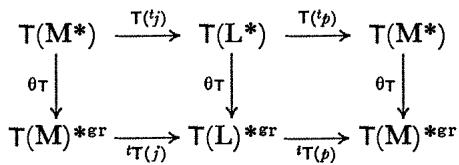
\includegraphics[keepaspectratio]{images/part004_2d3cbe02.jpg}}

以及一个类似的交换图，其中 \(\mathsf{T}\) 被替换为 \(\bigwedge\) 。该命题随后由以下引理得出：

引理2. 设

\pandocbounded{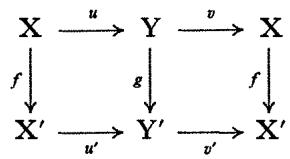
\includegraphics[keepaspectratio]{images/part004_a09507a7.jpg}}

是一个集合与映射的交换图，使得 \(v \circ u\) 和 \(v' \circ u'\) 分别是 \(X\) 和 \(X'\) 的恒等映射。那么，若 \(g\) 是单射（相应地，满射、双射），则 \(f\) 亦然。

u 是单射，因为 \(v \circ u\) 是；因此，若 g 是单射， \(u' \circ f = g \circ u\) 是单射，从而 f 是单射。类似地 \(v'\) 是满射，因为 \(v' \circ u'\) 是；因此，若 g 是满射， \(f \circ v = v' \circ g\) 是满射，从而 f 是满射。

命题7的最后断言由以下事实得出： \(\bigwedge (\mathbf{M})\) 此时是一个有限生成的 A-模（§ 7，第 3 号，命题 6 及 II，§ 11，第 6 号，注记）。

我们现在考察关于同态 \(\theta_{\mathsf{S}}\) （当 \(\mathbf{M}\) 是投射的且有限生成时）可以说些什么。首先假设 \(\mathbf{M}\) 具有有限基 \((e_i)_{1\leq i\leq m}\) 。在本章开头的记号中，A-模 \(\mathbf{S}^n (\mathbf{M})\) 以元素族 \(e^{\alpha}\) （满足 \(|\alpha | = n\) ）为基。设 \(u_{\alpha}\) （对于 \(|\alpha | = n\) ）表示指标为 \(\alpha\) 的元素，位于 \((\mathbf{S}^n (\mathbf{M}))^*\) 的对偶于 \((e^{\alpha})\) 的基中。元素 \(u_{\alpha}\) （对于 \(\alpha \in \mathbf{N}^m\) ）因此构成代数 \(\mathbf{S}(\mathbf{M})^{*\mathrm{gr}}\) 的基，我们将显式给出这个基的乘法表。我们记

\[
u _ {\alpha} u _ {\beta} = \sum_ {\gamma \in \mathbf {N} ^ {m}} a _ {\alpha \beta \gamma} u _ {\gamma} \quad \text { with } a _ {\alpha \beta \gamma} \in \mathrm{A}.
\]

那么根据定义

\[
a _ {\alpha \beta \gamma} = \langle u _ {\alpha} u _ {\beta}, e ^ {\gamma} \rangle = m ((u _ {\alpha} \otimes u _ {\beta}) (c (e ^ {\gamma}))),
\]

（其中 \(m: \mathbf{A} \otimes \mathbf{A} \to \mathbf{A}\) 定义 \(\mathbf{A}\) 上的乘法， \(c\) 是 \(\mathsf{S}(\mathbf{M})\) 的余积。换言之， \(a_{\alpha \beta \gamma}\) 正是 \(e^{\alpha} \otimes e^{\beta}\) 的系数（当 \(c(e^{\gamma})\) 用 \(\mathsf{S}(\mathbf{M})\otimes \mathsf{S}(\mathbf{M})\) 的由 \(e^{\xi}\otimes e^{\eta}\) 组成的基表示时），其中 \(\xi\) 和 \(\eta\) 遍历 \(\mathbf{N}^m\) 。但由于 \(c\) 是代数同态，

\[
c (e ^ {\gamma}) = \prod_ {i = 1} ^ {m} (c (e _ {i})) ^ {\gamma_ {i}} = \prod_ {i = 1} ^ {m} (e _ {i} \otimes 1 + 1 \otimes e _ {i}) ^ {\gamma_ {i}}
\]

根据第1号公式 (4)，这给出

\[
c (e ^ {\gamma}) = \sum_ {\xi + \eta = \gamma} (\xi , \eta) e ^ {\xi} \otimes e ^ {\eta}\tag{31}
\]

其中我们记

\[
((\xi , \eta)) = \prod_ {i = 1} ^ {n} \frac {(\xi_ {i} + \eta_ {i}) !}{\xi_ {i} ! \eta_ {i} !} \quad (\text { cf.   } \S 10, \text {   no.   } 4, \text {   formula   (18) }).\tag{32}
\]

因此我们得到乘法表

\[
u _ {\alpha} u _ {\beta} = ((\alpha , \beta)) u _ {\alpha + \beta}.\tag{33}
\]

另一方面，如果 \((e_i^*)_{1\leq i\leq m}\) 是 \(\mathbf{M}^*\) 的、对偶于 \((e_i)\) 的基，则由公式 (29 bis) 可知，对所有 \(\alpha \in \mathbf{N}^m\) ，

\[
\theta_ {S} (e ^ {* \alpha}) = \alpha ! u _ {\alpha}\tag{34}
\]

在 §6 第6号的记号中。因此同态 \(\theta_{\mathsf{S}}\) 是双射当且仅当诸 \(\alpha!u_{\alpha}\) 构成 \(\mathsf{S}(\mathbf{M})^{*\mathrm{gr}}\) 的一组基，亦即诸元素 \(\alpha!1\) 均可逆。

命题8. 假设环 A 是有理数域 Q 上的代数；那么，对于每个有限生成的投射 A-模 M，同态

\[
\theta_ {\mathsf {S}}: S (M ^ {*}) \rightarrow S (M) ^ {* \mathrm{gr}}
\]

是双射。

这相当于在M有限生成且自由的情形下证明；我们像命题7的证明中那样，利用引理2从这一情形过渡到一般情形。

注记。设 M 为一个 A-模，且 \(\rho: \mathbf{A} \to \mathbf{B}\) 为一个交换环同态。则存在一个分次 B-代数同态的交换图

\[
\begin{array}{l} \mathsf {T} ((\mathbf {M} ^ {*}) _ {(B)}) \longrightarrow (\mathsf {T} (\mathbf {M}) ^ {* \mathrm{gr}}) _ {(B)} \\ \mathsf {T} (\upsilon_ {\mathbf {M}}) \Biggl \downarrow \qquad \qquad \qquad \qquad \qquad \qquad \qquad \qquad \qquad \Biggl \downarrow \upsilon_ {\mathbf {T} (\mathbf {M})} \\ \mathsf {T} ((\mathbf {M} _ {(B)}) ^ {*}) \xrightarrow [ \theta_ {\mathsf {T}} ]{} \mathsf {T} (\mathbf {M} _ {(B)}) ^ {* \mathrm{gr}} \end{array}
\]

其中第一行是由同态 \(\theta_{\mathsf{T}}\otimes 1_{\mathsf{B}}\colon \mathsf{T}(\mathbf{M}^{*})\otimes_{\mathbf{A}}\mathbf{B}\to \mathsf{T}(\mathbf{M})^{*\mathrm{gr}}\) 与典范同构

\[
\mathsf {T} ((\mathbf {M} ^ {*}) _ {(\mathbf {B})}) \rightarrow \mathsf {T} (\mathbf {M} ^ {*}) \otimes_ {\mathbf {A}} \mathbf {B}
\]

（§ 5，第 3 号，命题 5）复合而成的同态。利用公式 (28) 及同态 \(\upsilon_{\mathbf{E}}\) （II，§ 5，第 4 号）的定义，可立即验证此图表是交换的。当 \(\mathbf{M}\) 是有限生成的投射 A-模时， \(\mathbf{M}_{(\mathbf{B})}\) 是有限生成的投射 B-模（II，§ 5，第 1 号，命题 4 的推论），且上述图表中的所有同态都是双射（命题 7 及 II，§ 5，第 4 号，命题 8）。存在类似的交换图，其中 \(\mathsf{T}\) 被替换为 \(\mathsf{S}\) 或 \(\bigwedge\) ；关于 \(\bigwedge\) 的那个图当 \(\mathbf{M}\) 是投射的且有限生成时也由双射同态组成（命题 7）；若进一步 \(\mathbf{A}\) 是 \(\mathbf{Q}\) 上的代数，则关于 \(\mathsf{S}\) 的图也由双射同态组成（命题 8）。

\subsection{内乘：代数情形}

设 \(E = \bigoplus_{p \geqslant 0} E_p\) 是一个 N 型分次 A-代数，P 是一个 Z 型分次 A-模；对每个齐次元素 \(x \in E_p\) ，用 \(x\) 左乘是 E 到自身的 A-线性映射 \(e(x)\) ，它是 \(p\) 次分次映射。对每个元素 \(u \in \text{Homgr}_A(E, P)\) ， \(u\) 被 \(x\) 的右内乘记作 \(u \llcorner x\) ，它就是元素 \(u \circ e(x)\) （属于 \(\text{Homgr}_A(E, P)\) ）。我们还记 \((i(x))(u) = u \llcorner x\) ，于是可见 \(i(x)\) 是 \(p\) 次分次自同态（分次 A-模 \(\text{Homgr}_A(E, P)\) 的）。若现在 \(x = \sum_{p \geqslant 0} x_p\) 是 E 的任意元素（其中 \(x_p \in E_p\) （对一切 \(p \geqslant 0\) ），且 \(x_p = 0\) （除 \(p\) 的有限个值外）），我们记 \(i(x) = \sum_{p=0}^{\infty} i(x_p)\) ，它因此是 A-模 \(\text{Homgr}_A(E, P)\) 的自同态。

为了记住在表达式 \(u \llcorner x\) 中哪个元素“作用”于另一个元素，注意“作用”于 u 的元素 x 位于 \(\llcorner\) 中水平线的自由端。

代数 E 的结合性转化为关系 \(e(xy) = e(x) \circ e(y)\) （对齐次的 x, y）；因此，根据 \(i(x)\) 的定义，

\[
i (x y) = i (y) \circ i (x)\tag{35}
\]

首先对齐次的 \(x, y\) ，然后通过线性性，对 E 中任意的 \(x, y\) ；这也可以写成

\[
(u \llcorner x) \llcorner y = u \llcorner (x y)\tag{36}
\]

对于 \(x, y\) （在 \(\mathbf{E}\) 中）及 \(u \in \operatorname{Homgr}_{\mathbf{A}}(\mathbf{E}, \mathbf{P})\) ；另一方面，显然 \(i(1)\) 是恒等映射（因为由 \(e(1) = 1_{\mathbf{E}}\) 即得），且 \(x \mapsto i(x)\) 是 A-线性的，于是可以看出，外合成律 \((x, u) \mapsto u \llcorner x\) （ \(x \in \mathbf{E}\) ， \(u \in \operatorname{Homgr}_{\mathbf{A}}(\mathbf{E}, \mathbf{P})\) ）与加法一起，在 \(\operatorname{Homgr}_{\mathbf{A}}(\mathbf{E}, \mathbf{P})\) 上定义了一个右 E-模结构。

特别地，我们考虑 P = A 的情形， \(\operatorname{Homgr}_{\mathbf{A}}(\mathbf{E}, \mathbf{P})\) 在此情形下是 E 的分次对偶 \(E^{*gr}\) ； \(i(x)\) 则是 A-线性映射 \(e(x)\) 的分次转置（II，§11，第6号），换言之，对 E 中所有 x, y 及 \(u \in E^{*gr}\) ，

\[
\langle u \llcorner x, y \rangle = \langle u, x y \rangle .\tag{37}
\]

按照本段开头的约定，注意，若 \(x \in E_{p}\) ，则 \(i(x)\) 是 \(E^{*gr}\) 的 -p 次自同态。

对每个齐次元素 \(x \in \mathbf{E}_p\) ，用 \(x\) 右乘类似地记作 \(e'(x)\) ，而元素 \(u \circ e'(x)\) （属于 \(\operatorname{Homgr}_{\mathbf{A}}(\mathbf{E}, \mathbf{P})\) ）称为 \(u\) 被 \(x\) 的左内乘，记作 \(x \lrcorner u\) ；我们记 \(i'(x) = x \lrcorner u\) ，于是 \(i'(x)\) 是 \(\operatorname{Homgr}_{\mathbf{A}}(\mathbf{E}, \mathbf{P})\) 的 \(p\) 次分次自同态；如上所述，此定义可推广到 \(x\) 是 \(\mathbf{E}\) 的任意元素的情形。由于这时 \(e'(xy) = e'(y)e'(x)\) ，

\[
i ^ {\prime} (x y) = i ^ {\prime} (x) \circ i ^ {\prime} (y)\tag{38}
\]

也可以写作

\[
x \lrcorner (y \lrcorner u) = (x y) \lrcorner u\tag{39}
\]

并且表明外合成律 \((x,u)\mapsto x\lrcorner u\) 与加法一起，在 \(\operatorname{Homgr}_{\mathbf{A}}(\operatorname{E},\operatorname{P})\) 上定义了一个左 E-模结构。另一方面，E 的结合性蕴含 \(e(x)\circ e'(y)=e'(y)\circ e(x)\) （对 E 中齐次的 x,y），由此得到关系式

\[
(y \lrcorner u) \llcorner x = y \lrcorner (u \llcorner x)\tag{40}
\]

从而使 \(\mathrm{Homgr}_{\mathbf{A}}(\mathbf{E},\mathbf{P})\) 上的两个外合成律在此集合上定义一个 (E, E)-双模结构（II，§ 1，第14号）。

当我们取 \(\mathbf{P} = \mathbf{A}\) 时， \(i'(x)\) 是 \(e'(x)\) 的分次转置；换言之，对所有 \(x, y\) （在 \(\mathbf{E}\) 中）及 \(u \in \mathbf{E}^{*\mathrm{gr}}\) ，

\[
\langle y, x \lrcorner u \rangle = \langle y x, u \rangle .\tag{41}
\]

当分次代数 E 是交换的时，显然 \(u \llcorner x = x \lrcorner u\) 。当 E 是反交换的且 P = A 时，则对于 \(x \in E_{p}\) 、 \(y \in E_{r}\) 和 \(u \in E_{q}^{*}\) ，有 \(yx = (-1)^{pr}xy\) ，由此，由 (37) 和 (41) 得 \(\langle u \llcorner x, y \rangle = (-1)^{pr}\langle y, x \lrcorner u \rangle\) 。但由于该关系的两边除 r = q - p 外均为零，

\[
x \lrcorner u = (- 1) ^ {p (q - p)} u \llcorner x.
\]

设 F 为另一个分次 A-代数，且 \(\phi: E \to F\) 为分次代数的一个 A-同态；则 \(\tilde{\phi} = \operatorname{Hom}(\phi, 1_{P}): \operatorname{Homgr}_{A}(F, P) \to \operatorname{Homgr}_{A}(E, P)\) 是 0 次的分次 A-同态；根据定义，对于 E 中的 \(x, y\) 及 \(u \in \operatorname{Homgr}_{A}(F, P)\) ，

\[
\begin{array}{r l} (\tilde {\phi} (u \llcorner \phi (x))) (y) & = (u \llcorner \phi (x)) (\phi (y)) \\ & = u (\phi (x) \phi (y)) = u (\phi (x y)) = (\tilde {\phi} (u)) (x y) = (\tilde {\phi} (u) \llcorner x) (y) \end{array}
\]

或等价地

\[
\tilde {\phi} (u \llcorner \phi (x)) = \tilde {\phi} (u) \llcorner x\tag{42}
\]

并且类似地

\[
\tilde {\phi} (\phi (x) \lrcorner u) = x \lrcorner \tilde {\phi} (u).\tag{43}
\]

换句话说，当 \(\operatorname{Homgr}_{\mathbf{A}}(\mathbf{F}, \mathbf{P})\) 借助环同态 \(\phi: \mathbf{E} \to \mathbf{F}\) 被视为 (E, E)-双模时，可以看出 \(\tilde{\phi}\) 是一个 (E, E)-双模同态（或者是把 (F, F)-双模 \(\operatorname{Homgr}_{\mathbf{A}}(\mathbf{F}, \mathbf{P})\) 映入 (E, E)-双模 \(\operatorname{Homgr}_{\mathbf{A}}(\mathbf{E}, \mathbf{P})\) 的 E-同态）。

例子。特别地，当 E 是分次代数 \(\mathsf{T}(\mathbf{M})\) 、 \(\mathsf{S}(\mathbf{M})\) 或 \(\bigwedge(\mathbf{M})\) 之一（其中 M 是一个 A-模），而 P 是一个 A-模（带有平凡分次）时，上述内容可以应用。为了显式求出如此得到的双模结构，注意 \(\operatorname{Homgr}_{\mathbf{A}}(\mathsf{T}(\mathbf{M}),\mathbf{P})\) （相应地 \(\operatorname{Homgr}_{\mathbf{A}}(\mathsf{S}(\mathbf{M}),\mathbf{P})\) 、 \(\operatorname{Homgr}_{\mathbf{A}}(\bigwedge(\mathbf{M}),\mathbf{P})\) ）中 -n 次的元素与从 \(M^{n}\) 到 P 的 n 重线性映射（相应地，对称 n 重线性映射、交错 n 重线性映射）等同。只需表出乘积

\[
f \llcorner (x _ {1} \otimes x _ {2} \otimes \dots \otimes x _ {p})
\]

\((\text{resp. } f \llcorner (x_1 x_2 \ldots x_p), \text{ resp. } f \llcorner (x_1 \wedge x_2 \wedge \dots \wedge x_p))\) （对 M 中元素的每个有限序列 \((x_i)_{1 \leq i \leq p}\) ）以及左内乘的类似表达式。由定义立即得出

\[
f \llcorner (x _ {1} \otimes x _ {2} \otimes \dots \otimes x _ {p}) = (x _ {1} \otimes x _ {2} \otimes \dots \otimes x _ {p}) \lrcorner f = 0\tag{44}
\]

若 \(p > n\) ，并且对于 \(p \leqslant n, f \llcorner (x_1 \otimes x_2 \otimes \dots \otimes x_p)\) （相应地

\[
\left(x _ {1} \otimes x _ {2} \otimes \dots \otimes x _ {p}\right) \lrcorner f)
\]

是由下式定义的 \((n - p)\) -线性映射：

\[
\left\{ \begin{array}{l} (f \llcorner (x _ {1} \otimes x _ {2} \otimes \dots \otimes x _ {p})) (y _ {1}, \ldots , y _ {n - p}) \\ = f (x _ {1}, \ldots , x _ {p}, y _ {1}, \ldots , y _ {n - p}) \\ ((x _ {1} \otimes x _ {2} \otimes \dots \otimes x _ {p}) \lrcorner f) (y _ {1}, \ldots , y _ {n - p}) \\ = f (y _ {1}, \ldots , y _ {n - p}, x _ {1}, \ldots , x _ {p}). \end{array} \right.\tag{45}
\]

对于 \(p > n\) ，在 \(\operatorname{Homgr}_{\mathbf{A}}(\mathsf{S}(\mathbf{M}), \mathbf{P})\) （相应地 \(\operatorname{Homgr}_{\mathbf{A}}(\bigwedge(\mathbf{M}), \mathbf{P})\) ）中也有公式 (44)，其中 \(x_1 \otimes x_2 \otimes \cdots \otimes x_p\) 替换为 \(x_1x_2 \ldots x_p\) （相应地 \(x_1 \wedge x_2 \wedge \cdots \wedge x_p\) ）。对于 \(p \leqslant n\) ，在 (45) 中进行相同的替换，就定义了对称 \((n - p)\) -线性映射 \(f \llcorner (x_1x_2 \ldots x_p)\) 和 \((x_1x_2 \ldots x_p) \lrcorner f\) （相应地，交错 \((n - p)\) -线性映射

\[
f \llcorner (x _ {1} \wedge x _ {2} \wedge \dots \wedge x _ {p}) \quad \text { and } \quad (x _ {1} \wedge x _ {2} \wedge \dots \wedge x _ {p}) \lrcorner f).
\]

当 \(n = p\) 时，上述乘积等于 \(\mathbf{M}\) 上等于 \(f(x_{1},\ldots ,x_{p})\) 的常值函数。

若 \(u: \mathbf{M} \to \mathbf{N}\) 是 A-模同态，则 \(\mathsf{T}(u): \mathsf{T}(\mathbf{M}) \to \mathsf{T}(\mathbf{N})\) 是分次 A-代数同态，于是由我们上面所见可知， \((\mathsf{T}(u))^{\sim}\) 是 \(\mathsf{T}(\mathbf{M})\) -同态，把 \((\mathsf{T}(\mathbf{N}), \mathsf{T}(\mathbf{N}))\) -双模 \(\operatorname{Homgr}_{\mathbf{A}}(\mathsf{T}(\mathbf{N}), \mathbf{P})\) 映入 \((\mathsf{T}(\mathbf{M}), \mathsf{T}(\mathbf{M}))\) -双模 \(\operatorname{Homgr}_{\mathbf{A}}(\mathsf{T}(\mathbf{M}), \mathbf{P})\) ，相对于环同态 \(\mathsf{T}(u)\) 。对 \((\mathbf{S}(u))^{\sim}\) 和 \((\bigwedge(u))^{\sim}\) 有类似的结果。
% semantic-fragments: legacy-input-seam
\relax{}
\subsection{内乘：余代数情形}

设 \(E = \bigoplus_{p \geq 0} E_p\) 是一个余结合、余单位的分次余代数。那么我们知道（第 2 号，命题 1 和 3），分次对偶 \(E^{*gr}\)（按照本段开头关于分次的约定）具有 A 上的一个 N 型分次代数结构，该代数中两个元素 \(u, v\) 的乘积由 \(uv = m \circ (u \otimes v) \circ c\) 定义，其中 \(c: E \to E \otimes_A E\) 是余积，而 \(m: A \otimes_A A \to A\) 定义乘法。换言之，若对 \(x \in E\) 有 \(c(x) = \sum_i y_i \otimes z_i\) ，则我们可以写成（将 \(A \otimes_A E\) 与 \(E\) 典范地等同）

\[
\begin{array}{r l} \langle x, u v \rangle = (u v) (x) & = \sum_ {i} u (y _ {i}) v (z _ {i}) = v \left(\sum_ {i} u (y _ {i}) z _ {i}\right) \\ & = v (((u \otimes 1 _ {\mathbb {E}}) \circ c) (x)) = \langle ((u \otimes 1 _ {\mathbb {E}}) \circ c) (x), v \rangle . \end{array}
\]

这可以解释为：对 \(E^{*gr}\) 中所有次数为 p 的齐次元素 u，左乘 \(e(u): v \mapsto uv\) 在 \(E^{*gr}\) 中是 E 的次数为 -p 的分次自同态的分次转置

\[
i (u) = (u \otimes 1 _ {\mathrm{E}}) \circ c\tag{46}
\]

因此，在上述记号中，

\[
(i (u)) (x) = \sum_ {i} u (y _ {i}) z _ {i}.
\]

公式 (46) 同样定义了一个元素 \(i(u)\in\mathrm{Endgr}_{\mathbf{A}}(\mathbf{E})\)（对每个元素 \(u\in\mathbf{E}^{*\mathbf{g}\mathbf{r}}\) 而言）；对所有 \(x\in\mathbf{E}\) 及所有 \(u\in\mathbf{E}^{*\mathbf{g}\mathbf{r}}\) ，我们记

\[
x \llcorner u = (i (u)) (x)\tag{47}
\]

使得，对 E*gr 中的 u 和 v，

\[
\langle x, u v \rangle = \langle x \llcorner u, v \rangle .
\]

E 的元素 \(x \llcorner u\) 称为 x 被 u 的右内乘。

这里再次将“作用于”x的元素u放在L中水平线的自由端。

对任意两个元素 \(u, v\)（属于 \(\mathbf{E}^{*\mathrm{gr}}\)），

\[
x \llcorner (u v) = (x \llcorner u) \llcorner v,\tag{48}
\]

换句话说

\[
i (u v) = i (v) \circ i (u).
\]

如上所述，令 \(c(x) = \sum_{i} y_{i} \otimes z_{i}\) ，则有 \(x \llcorner (uv) = \sum_{i} (uv)(y_{i})z_{i}\) 。若

\[
c (y _ {i}) = \sum_ {j} y _ {i j} ^ {\prime} \otimes y _ {i j} ^ {\prime \prime},
\]

那么

\[
x \llcorner (u v) = \sum_ {i, j} u \left(y _ {i j} ^ {\prime}\right) v \left(y _ {i j} ^ {\prime \prime}\right) z _ {i}.\tag{49}
\]

另一方面，如果 \(c(z_{i}) = \sum_{k} z_{ik}' \otimes z_{ik}''\) ，则

\[
(x \llcorner u) \llcorner v = \sum_ {i, k} u (y _ {i}) v (z _ {i k} ^ {\prime}) z _ {i k} ^ {\prime \prime}.\tag{50}
\]

现在，E 的余结合性表明（第 2 号，命题 1）

\[
\sum_ {i, j} y _ {i j} ^ {\prime} \otimes y _ {i j} ^ {\prime \prime} \otimes z _ {i} = \sum_ {i, k} y _ {i} \otimes z _ {i k} ^ {\prime} \otimes z _ {i k} ^ {\prime \prime}\tag{51}
\]

而表达式 (49) 与 (50) 的相等性来自如下事实：它们分别是 (51) 式左、右两端在从 \(E \otimes E \otimes E\) 到 E 的线性映射 f 下的像，其中 \(f(x \otimes y \otimes z) = u(x)v(y)z\) 。

另一方面，我们回顾（第 2 号，命题 3），代数 \(\mathbf{E}^{*\mathrm{gr}}\) 的单位元是线性形式 \(e: x \mapsto \gamma(x).1\) ；因此

\[
x \llcorner e = \sum_ {i} \gamma (y _ {i}) z _ {i} = x
\]

这是余单位定义的直接推论。由于映射 \(u \mapsto i(u)\) 是线性的，可以看出外合成律 \((u, x) \mapsto x \llcorner u\) 在 E 上定义了一个右 E*gr-模结构。

类似地，我们对所有 \(u \in \mathrm{E}^{*\mathbf{g}\mathbf{r}}\) 定义 \(\mathbf{E}\) 的自同态

\[
i ^ {\prime} (u) = \left(1 _ {E} \otimes u\right) \circ c\tag{52}
\]

并且，对所有 \(x \in \mathbf{E}\) ，我们记

\[
\left(i ^ {\prime} (u)\right) (x) = u \lrcorner x\tag{53}
\]

并且 E 的这个元素称为 x 被 u 的左内乘。如前所述可以看出，外合成律 \((u, v) \mapsto u \lrcorner x\) 在 E 上定义了一个左 \(\mathrm{E}^{*gr}\)-模结构。此外，这两个结构是相容的，换言之，

\[
(u \lrcorner x) \llcorner v = u \lrcorner (x \llcorner v)\tag{54}
\]

这对 E*gr 中的 \(u, v\)（II，§ 1，第 14 号）成立。采用与上述相同的记号，(54) 的左边是 \(\sum_{i,j} u(z_i) v(y_{ij}') y_{ij}''\) ，右边是 \(\sum_{i,k} v(y_i) u(z_{ik}') z_{ik}''\) ；它们的相等性来自如下事实：它们分别是 (51) 式左、右两端在从 E ⊗ E ⊗ E 到 E 的线性映射 \(g\) 下的像，其中 \(g(x \otimes y \otimes z) = v(x) u(z)y\) 。

因此可以看出，E 上的两个外合成律在此集合上定义了一个 \((\mathrm{E}^{*}\mathrm{gr}, \mathrm{E}^{*}\mathrm{gr})\)-双模结构。

当余代数 E 余交换时，则 \(u \lrcorner x = x \llcorner u\) ，其中 \(x \in \mathbf{E}\) 和 \(u \in \mathrm{E}^{*\mathrm{gr}}\) 任取；当它余反交换（§ 4，第 9 号）且 \(u \in \mathrm{E}_p^*\) 、 \(x \in \mathrm{E}_q\) 时，我们可以写成 \(c(x) = \sum_{0 \leqslant j \leqslant q} \left( \sum_i y_{ij} \otimes z_{i,q-j} \right)\) ，其中 \(y_{ij}\) 和 \(z_{ij}\) 都属于 \(\mathrm{E}_j\) （对每个 \(j\) ），于是由假设

\[
\sum_ {i} z _ {i j} \otimes y _ {i, q - j} = (- 1) ^ {j (q - j)} \sum_ {i} y _ {i j} \otimes z _ {i, q - j}.
\]

由定义， \(x \llcorner u = \sum_{0 \leqslant j \leqslant q} \left( \sum_{i} u(y_{ij}) z_{i,q-j} \right)\) 和

\[
u \lrcorner x = \sum_ {0 \leqslant j \leqslant q} \left(\sum_ {i} u (z _ {i, q - j}) y _ {i j}\right).
\]

由于 \(u(y_{ij}) = 0\) （相应地 \(u(z_{i,q-j}) = 0\) ），除非 \(j = p\) （相应地 \(q - j = p\) ），由上述可知 \(u \lrcorner x = (-1)^{p(q-p)}x \llcorner u\) 。

最后，设 \(\phi: \mathrm{E} \to \mathrm{F}\) 是一个分次余代数态射；那么已经看到（第 2 号），分次转置 \(^t\phi: \mathrm{F}^{*\mathrm{gr}} \to \mathrm{E}^{*\mathrm{gr}}\) 是一个分次代数同态；因此，对 \(x \in \mathrm{E}, u, v\) （属于 \(\mathrm{F}^{*\mathrm{gr}}\) ），

\[
\begin{array}{r l} \langle \phi (x \llcorner {} ^ {t} \phi (u)), v \rangle & = \langle x \llcorner {} ^ {t} \phi (u), ^ {t} \phi (v) \rangle = \langle x, ^ {t} \phi (u) ^ {t} \phi (v) \rangle = \langle x, ^ {t} \phi (u v) \rangle \\ & = \langle \phi (x), u v \rangle = \langle \phi (x) \llcorner u, v \rangle \end{array}
\]

从而

\[
\phi (x) \llcorner u = \phi (x \llcorner {} ^ {t} \phi (u));\tag{55}
\]

并且类似地

\[
u \lrcorner \phi (x) = \phi (^ {t} \phi (u) \lrcorner x).\tag{56}
\]

换言之， \(\phi\) 是一个 \(\mathbf{F}^{*\mathrm{gr}}\) -同态，从 \((\mathrm{E}^{*\mathrm{gr}}, \mathrm{E}^{*\mathrm{gr}})\) -双模 E 到 \((\mathrm{F}^{*\mathrm{gr}}, \mathrm{F}^{*\mathrm{gr}})\) -双模 F，相对于环同态

\[
{ } ^ { t } \phi : \mathrm{F} ^ { * \mathrm{gr} } \rightarrow \mathrm{E} ^ { * \mathrm{gr} } .
\]

例子。特别地，当 E 是分次余代数 \(\mathsf{T}(\mathbf{M})\) , \(\mathsf{S}(\mathbf{M})\) 或 \(\bigwedge(\mathbf{M})\) 之一（M 为一个 A-模）（第 1 号，例 5、6 和 7）时，可以应用上述内容。为了显式求出如此得到的双模结构，我们再次将 \(\mathsf{T}(\mathbf{M})^{*\mathbf{g}\mathbf{r}}\) （相应地 \(\mathsf{S}(\mathbf{M})^{*\mathbf{g}\mathbf{r}}\) ，相应地 \(\bigwedge(\mathbf{M})^{*\mathbf{g}\mathbf{r}}\) ）中次数为 n 的齐次元素 f 等同于 \(M^{n}\) 上的一个 n-线性形式（相应地，对称 n-线性形式；相应地，交错 n-线性形式，也称为 n-形式）。只需就 M 的元素表出这些乘积

\[
\left(x _ {1} \otimes x _ {2} \otimes \dots \otimes x _ {p}\right) \llcorner f (\text { resp. } (x _ {1} x _ {2} \dots x _ {p}) \llcorner f,
\]

（相应地 \((x_{1} \wedge x_{2} \wedge \cdots \wedge x_{p}) \llcorner f)\) ），对 M 中元素的每一有限序列 \((x_{i})_{1 \leqslant i \leqslant p}\) ，以及左内乘的类似表达式。现在，定义 (46) 和 (52) 以及第 1 号的公式 (3)、(6) 和 (9) 分别给出：

\[
\left\{ \begin{array}{l} (x _ {1} \otimes x _ {2} \otimes \dots \otimes x _ {p}) \llcorner f = f \lrcorner (x _ {1} \otimes x _ {2} \otimes \dots \otimes x _ {p}) = 0 \\ (x _ {1} x _ {2} \ldots x _ {p}) \llcorner f = f \lrcorner (x _ {1} x _ {2} \ldots x _ {p}) = 0 \quad \text {for} \quad p <   n. \\ (x _ {1} \wedge x _ {2} \wedge \dots \wedge x _ {p}) \llcorner f = f \lrcorner (x _ {1} \wedge x _ {2} \wedge \dots \wedge x _ {p}) = 0 \end{array} \right.\tag{57}
\]

对 \(p \geqslant n\) ，我们分别有

\begin{enumerate}
\def\labelenumi{(\arabic{enumi})}
\setcounter{enumi}{57}
\tightlist
\item
\end{enumerate}

\[
\left(x _ {1} \otimes x _ {2} \otimes \dots \otimes x _ {p}\right) \llcorner f = f \left(x _ {1}, \dots , x _ {n}\right) x _ {n + 1} \otimes \dots \otimes x _ {p}\tag{59}
\]

\[
\left(x _ {1} x _ {2} \dots x _ {p}\right) \llcorner f = \sum_ {\sigma} f \left(x _ {\sigma (1)}, \dots , x _ {\sigma (n)}\right) x _ {\sigma (n + 1)} \dots x _ {\sigma (p)}\tag{60}
\]

\[
\left(x _ {1} \wedge x _ {2} \wedge \dots \wedge x _ {p}\right) \llcorner f = \sum_ {\sigma} \varepsilon_ {\sigma} f \left(x _ {\sigma (1)}, \dots , x _ {\sigma (n)}\right) x _ {\sigma (n + 1)} \wedge \dots \wedge x _ {\sigma (p)}
\]

（其中，在 (59) 和 (60) 中，求和是对排列 \(\sigma \in \mathfrak{S}_p\) 中在每个区间 \([1, n]\) 和 \([n + 1, p]\) （均为 \(\mathbf{N}\) 的区间）上递增的那些进行的）；并且类似地

\begin{enumerate}
\def\labelenumi{(\arabic{enumi})}
\setcounter{enumi}{60}
\tightlist
\item
\end{enumerate}

\[
f \lrcorner (x _ {1} \otimes x _ {2} \otimes \dots \otimes x _ {p}) = f (x _ {p - n + 1}, \dots , x _ {p}) x _ {1} \otimes x _ {2} \otimes \dots \otimes x _ {p - n}\tag{62}
\]

\[
f \lrcorner (x _ {1} x _ {2} \dots x _ {p}) = \sum_ {\sigma} f (x _ {\sigma (p - n + 1)}, \dots , x _ {\sigma (p)}) x _ {\sigma (1)} \dots x _ {\sigma (p - n)}\tag{63}
\]

\[
f \lrcorner (x _ {1} \wedge x _ {2} \wedge \dots \wedge x _ {p}) =
\]

\[
\sum_ {\sigma} \varepsilon_ {\sigma} f (x _ {\sigma (p - n + 1)}, \dots , x _ {\sigma (p)}) x _ {\sigma (1)} \wedge \dots \wedge x _ {\sigma (p - n)}
\]

（其中，在 (62) 和 (63) 中，求和是对排列 \(\sigma \in \mathfrak{S}_p\) 中在每个区间 \([1, p - n]\) 和 \([p - n + 1, p]\) （均为 \(\mathbf{N}\) 的区间）上递增的那些进行的）。

\subsection{内乘：双代数情形}

设 E 是一个分次双代数（相应地，斜分次双代数）（第 4 号，定义 3）；那么第 6 号和第 7 号的结果可以用来定义右（相应地，左）内乘 \(x \llcorner u \in \mathbf{E}\) 和 \(u \llcorner x \in \mathbf{E}^{*\mathbf{gr}}\) （相应地 \(u \lrcorner x \in \mathbf{E}\) 和 \(x \lrcorner u \in \mathbf{E}^{*\mathbf{gr}}\) )

这对所有 \(x \in \mathbf{E}\) 及所有 \(u \in \mathbf{E}^{*\mathbf{gr}}\) 进行。于是就在 E 上得到一个 (E, E)-双模结构和一个 \((\mathbf{E}^{*\mathbf{gr}}, \mathbf{E}^{*\mathbf{gr}})\)-双模结构。进一步：

命题 9. 设 E 是一个分次双代数（相应地，斜分次双代数）。对 E 中次数为 1 的每个元素 x，被 x 所作的左内乘和右内乘都是代数 E*gr 的导子（相应地，反导子）（§ 10，第 2 号）。

在第 6 号的记号中，对分次双代数（相应地，斜分次双代数）E 中每个次数为 1 的齐次元素 \(x\) ，

\[
c (x) = x \otimes 1 + 1 \otimes x,
\]

这由第 3 号命题 5 及 \(c\) 是次数为 0 的同态这一事实得出。首先假设 \(E\) 是分次双代数。对所有 \(y \in E\) ，根据定义

\[
\langle (u v) \llcorner x, y \rangle = \langle u v, x y \rangle = m ((u \otimes v) (c (x y)))
\]

并且由于 \(c\) 是代数同态， \(c(xy) = c(x)c(y)\) 。设 \(c(y) = \sum_{i} s_i \otimes t_i\) ，其中 \(s_i\) 和 \(t_i\) 属于 \(E\) ；因此

\[
c (x y) = \sum_ {i} (x s _ {i}) \otimes t _ {i} + \sum_ {i} s _ {i} \otimes (x t _ {i}).
\]

。因此 \(\langle (uv) \llcorner x, y \rangle = \sum_{i} u(xs_i)v(t_i) + \sum_{i} u(s_i)v(xt_i)\) 。但我们可以写

\[
\sum_ {i} u (x s _ {i}) v (t _ {i}) = m (((u \llcorner x) \otimes v) (c (y))) = \langle (u \llcorner x) v, y \rangle
\]

并且类似地

\[
\sum_ {i} u (s _ {i}) v (x t _ {i}) = m ((u \otimes (v \llcorner x)) (c (y))) = \langle u (v \llcorner x), y \rangle ,
\]

由此，回到用 \(i(x)\) 记内乘的记号，

\[
(i (x)) (u v) = ((i (x)) (u)) v + u ((i (x)) (v))\tag{64}
\]

，这证明了 \(i(x)\) 是 \(\mathbf{E}^{*}\mathbf{gr}\) 中的导子。

现在假设 \(\mathbf{E}\) 是斜分次双代数，并设 \(u\in \mathbf{E}_p^*\) , \(v\in \mathbf{E}_q^*\) 和 \(y\in \mathbf{E}_r\) ；则我们可以写

\[
c (y) = \sum_ {0 \leqslant j \leqslant r} \left(\sum_ {i} s _ {i j} \otimes t _ {i, r - j}\right)
\]

其中 \(s_{ij}\) 和 \(t_{ij}\) 属于 \(\mathbf{E}_j\) ；则由 \(\mathbf{E}^{\mathfrak{g}} \otimes_{\mathbf{A}} \mathbf{E}\) 中乘积的定义，

\[
c (x y) = c (x) c (y) = \sum_ {0 \leqslant j \leqslant r} \left(\sum_ {i} \left(x s _ {i j}\right) \otimes t _ {i, r - j} + (- 1) ^ {j} \sum_ {i} s _ {i j} \otimes \left(x t _ {i, r - j}\right)\right)
\]

从而这一次

\[
\langle (u v) \llcorner x, y \rangle = \sum_ {0 \leqslant j \leqslant r} \left(\sum_ {i} u \left(x s _ {i j}\right) v \left(t _ {i, r - j}\right) + (- 1) ^ {j} \sum_ {i} u \left(s _ {i j}\right) v \left(x t _ {i, r - j}\right)\right).
\]

同样地， \(\sum_{0\leqslant j\leqslant r}\left(\sum_{i}u(xs_{ij})v(t_{i,r - j})\right) = \langle (u\llcorner x)v,y\rangle\) 。另一方面， \(u(s_{ij}) = 0\) ，除非 \(j = -p\) ，因此我们也可以写成

\[
\sum_ {0 \leqslant j \leqslant r} (- 1) ^ {j} \left(\sum_ {i} u (s _ {i j}) v (x t _ {i, r - j})\right) = (- 1) ^ {p} \langle u (v \llcorner x), y \rangle .
\]

因此我们得出结论：

\[
(i (x)) (u v) = ((i (x)) (u)) v + (- 1) ^ {p} u ((i (x)) (v)),\tag{65}
\]

换言之， \(i(x)\) 是 \(\mathrm{E}^{*\mathrm{gr}}\) 中的反导子。关于 E 中次数为 1 的元素 \(x\) 所作的左内乘的断言，可类似地证明。

注记. (1) 设 E 是 A 上的分次双代数，且 N, N', N'' 是三个分次 A-模。设 m 是从 N × N' 到 N'' 的 A-双线性映射；对于 u \ensuremath{\in} Homgr\_A(E, N) 且 v \ensuremath{\in} Homgr\_A(E, N')，设 u.v 表示 E 到 N'' 的分次同态 m ∘ (u ⊗ v) ∘ c。另一方面，设 i(x) 表示由 x \ensuremath{\in} E 在 A-模 Homgr\_A(E, N), Homgr\_A(E, N') 与 Homgr\_A(E, N'\,') 中所作的（右或左）内乘。那么，若 x 的次数为 1，

\[
(i (x)) (u. v) = ((i (x)) (u)). v + u. ((i (x)) (v))
\]

这对所有 \(u \in \operatorname{Homgr}_{\mathbf{A}}(\mathbf{E}, \mathbf{N})\) 和 \(v \in \operatorname{Homgr}_{\mathbf{A}}(\mathbf{E}, \mathbf{N}')\) 成立。

在相同条件下，若 E 是斜分次双代数且 u 是次数为 p 的齐次元素，则

\[
(i (x)) (u. v) = ((i (x)) (u)). v + (- 1) ^ {p} u. ((i (x)) (v)).
\]

其证明与命题 9 中的相同。

\begin{enumerate}
\def\labelenumi{(\arabic{enumi})}
\setcounter{enumi}{1}
\tightlist
\item
  上述证明中的同一论证更一般地证明了：对所有 \(x \in \mathbf{E}\) ，若 \(c(x) = \sum_{j} x_j' \otimes x_{j'}'\) ，则对所有 \(u, v\) （属于 \(\mathbf{E}^{*\mathrm{gr}}\) ），“莱布尼茨公式”
\end{enumerate}

\[
(i (x)) (u v) = \sum_ {j} (i (x _ {j} ^ {\prime})) (u) \cdot (i (x _ {j} ^ {\prime \prime})) (v)
\]

成立。特别地，对分次双代数 E 的每个本原元素，即满足 \(c(x) = x \otimes 1 + 1 \otimes x\) 的元素， \(i(x)\) 是 \(\mathrm{E}^{*\mathrm{gr}}\) 的导子。

命题 10. 设 E 是一个分次双代数（相应地，斜分次双代数）。对 E*gr 中次数为 1 的任意元素 f，左内乘与右内乘都是代数 E 的导子（相应地，反导子）。

设 \(x \in \mathrm{E}_p, y \in \mathrm{E}_p\) ( \(p \geqslant 1, q \geqslant 1\) ）。根据第 3 号命题 5，我们可以写出

\[
c (x) = x \otimes 1 + \sum_ {1 \leqslant j \leqslant p - 1} \left(\sum_ {i} x _ {i j} ^ {\prime} \otimes x _ {i j, p - j} ^ {\prime \prime}\right) + 1 \otimes x
\]

\[
c (y) = y \otimes 1 + \sum_ {1 \leqslant k \leqslant q - 1} \left(\sum_ {i} y _ {i k} ^ {\prime} \otimes y _ {i, q - k} ^ {\prime \prime}\right) + 1 \otimes y
\]

（其中 \(x_{ij}'\) 和 \(x_{ij}''\) 属于 \(\mathrm{E}_j\) ， \(y_{ik}'\) 和 \(y_{ik}''\) 属于 \(\mathrm{E}_k\) 。若 \(\mathrm{E}\) 是分次双代数，则 \(c(xy) = c(x)c(y)\) 的属于 \(\mathrm{E}_1 \otimes \mathrm{E}\) 的分量等于

\[
\sum_ {i} x _ {i, 1} ^ {\prime} \otimes x _ {i, p - 1} ^ {\prime \prime} y + \sum_ {i} y _ {i, 1} ^ {\prime} \otimes x y _ {i, q - 1} ^ {\prime \prime}
\]

因此根据定义

\[
\begin{array}{r l} (x y) \llcorner f & = \sum_ {i} f (x _ {i, 1} ^ {\prime}) x _ {i, p - 1} ^ {\prime \prime} y + \sum_ {i} f (y _ {i, 1} ^ {\prime}) x y _ {i, q - 1} ^ {\prime \prime} \\ & = (x \llcorner f) y + x (y \llcorner f) \end{array}
\]

而由 \(f\) 所作的右内乘是一个导子。另一方面，若 \(E\) 是斜分次双代数，则 \(c(xy)\) 的属于 \(E_1 \otimes E\) 的分量等于

\[
\sum_ {i} x _ {i, 1} ^ {\prime} \otimes x _ {i, p - 1} ^ {\prime \prime} y + (- 1) ^ {p} \sum_ {i} y _ {i, 1} ^ {\prime} \otimes x y _ {i, q - 1} ^ {\prime \prime}
\]

而这一次我们得到

\[
(x y) \llcorner f = (x \llcorner f) y + (- 1) ^ {p} x (y \llcorner f)
\]

这表明 \(i(f)\) 是一个反导子。对由 \(f\) 所作的左内乘，论证类似。

例子。命题 9 和 10 特别适用于分次双代数 \(\mathsf{S}(\mathbf{M})\) 以及斜分次双代数 \(\bigwedge (\mathbf{M})\) 。由 \(\mathsf{S}(\mathbf{M})\) （相应地 \(\mathsf{S}(\mathbf{M})^{*\mathrm{gr}}\) ）中次数为 1 的元素所作的内乘是彼此可交换的导子，因为 \(\mathsf{S}(\mathbf{M})\) （相应地 \(\mathsf{S}(\mathbf{M})^{*\mathrm{gr}}\) ）是交换的。

类似地，由 \(\bigwedge (\mathbf{M})\) （相应地 \(\bigwedge (\mathbf{M})^{*\mathrm{gr}}\) ）中次数为 1 的元素所作的内乘是平方为零的反导子，因为代数 \(\bigwedge (\mathbf{M})\) （相应地 \(\bigwedge (\mathbf{M})^{*\mathrm{gr}}\) ）中次数为 1 的元素的平方为零。

\subsection{\texorpdfstring{\(\mathsf{T}(\mathbf{M})\) 与 \(\mathsf{T}(\mathbf{M}^{*})\)、\(\mathsf{S}(\mathbf{M})\) 与 \(\mathsf{S}(\mathbf{M}^{*})\)、\(\bigwedge(\mathbf{M})\) 与 \(\bigwedge(\mathbf{M}^{*})\) 之间的内乘}{T(M) 与 T(M*)、S(M) 与 S(M*)、wedge(M) 与 wedge(M*) 之间的内乘}}

右内乘在 \(\mathsf{T}(\mathbf{M})\) （相应地 \(\mathsf{S}(\mathbf{M})\) ，相应地 \(\bigwedge (\mathbf{M})\) ）上定义了代数 \(\mathsf{T}(\mathbf{M})^{*\mathfrak{g}\mathfrak{r}}\) （相应地 \(\mathsf{S}(\mathbf{M})^{*\mathfrak{g}\mathfrak{r}}\) ，相应地 \(\bigwedge (\mathbf{M})^{*\mathfrak{g}\mathfrak{r}}\) ）上的一个右模结构（第 7 号，例子）。利用第 5 号的典范同态 \(\theta_{\mathsf{T}}\) （相应地 \(\theta_{\mathsf{S}}\) ，相应地 \(\theta_{\wedge}\) ），我们得到

一个右 \(\mathsf{T}(\mathbf{M}^{*})\) -模结构，定义在 \(\mathsf{T}(\mathbf{M})\) 上

一个右 \(\mathbf{S}(\mathbf{M}^{*})\) -模结构，定义在 \(\mathbf{S}(\mathbf{M})\) 上

一个左 \(\bigwedge (\mathbf{M}^{*})\) -模结构，定义在 \(\bigwedge (\mathbf{M})\) 上。

这些结构中任何一个的外合成律也记为

\[
(z ^ {*}, t) \mapsto i (z ^ {*}). t
\]

（通过滥用语言）；我们也写作 \(t \llcorner z^*\) 以代替 \(i(z^*)\) . \(t\) ，在 \(\mathsf{T}(\mathbf{M})\) 或 \(\mathsf{S}(\mathbf{M})\) 的情形；另一方面，我们写作 \(z^* \lrcorner t\) ，在 \(\bigwedge (\mathbf{M})\) 的情形，并称其为 \(t\) 被 \(z^*\) 所作的左内乘，因为此时我们有一个左 \(\bigwedge (\mathbf{M}^*)\) -模法则。对齐次元素 \(z^*\) （次数为 \(n\) ）和齐次元素 \(t\) （次数为 \(p\) ），有 \(i(z^*)\) . \(t = 0\) （若 \(p < n\) ）；而对 \(x_i \in \mathbf{M} (1 \leqslant i \leqslant p)\) , \(x_j^* \in \mathbf{M}^* (1 \leqslant j \leqslant n)\) 及 \(p \geqslant n\) ，根据第 7 号的公式 (58)、(59) 和 (60)，

\[
\begin{array}{r l} i (x _ {1} ^ {*} \otimes x _ {2} ^ {*} \otimes \dots \otimes x _ {n} ^ {*}) \cdot (x _ {1} \otimes x _ {2} \otimes \dots \otimes x _ {p}) \\ & = \left(\prod_ {j = 1} ^ {n} \langle x _ {j} ^ {*}, x _ {j} \rangle\right) x _ {n + 1} \otimes \dots \otimes x _ {p} \end{array}\tag{66}
\]

\[
i \left(x _ {1} ^ {*} x _ {2} ^ {*} \dots x _ {n} ^ {*}\right). (x _ {1} x _ {2} \dots x _ {p}) = \sum_ {\sigma} \left(\prod_ {j = 1} ^ {n} \langle x _ {j} ^ {*}, x _ {\sigma (j)} \rangle\right) x _ {\sigma (n + 1)} \dots x _ {\sigma (p)}\tag{67}
\]

\[
\begin{array}{l} i \left(x _ {1} ^ {*} \wedge x _ {2} ^ {*} \wedge \dots \wedge x _ {n} ^ {*}\right). \left(x _ {1} \wedge x _ {2} \wedge \dots \wedge x _ {p}\right) \\ = (- 1) ^ {n (n - 1) / 2} \sum_ {\sigma} \varepsilon_ {\sigma} \left(\prod_ {j = 1} ^ {n} \langle x _ {j} ^ {*}, x _ {\sigma (j)} \rangle\right) x _ {\sigma (n + 1)} \wedge \dots \wedge x _ {\sigma (p)} \end{array}\tag{68}
\]

其中，在公式 (67) 和 (68) 中， \(\sigma\) 遍历排列 \(\sigma \in \mathfrak{S}_p\) 中在区间 \([1, n]\) 和 \([n + 1, p]\) 上递增的那些排列。我们也可以在内乘记号下写成

\[
\begin{array}{l l} \langle t \llcorner u ^ {*}, v ^ {*} \rangle = \langle t, \theta_ {\mathsf {T}} (u ^ {*} v ^ {*}) \rangle & \text {for} \quad t \in \mathsf {T} (\mathbf {M}), u ^ {*}, v ^ {*} \quad \text {in} \quad \mathsf {T} (\mathbf {M} ^ {*}) \\ \langle t \llcorner u ^ {*}, v ^ {*} \rangle = \langle t, \theta_ {\mathsf {S}} (u ^ {*} v ^ {*}) \rangle & \text {for} \quad t \in \mathsf {S} (\mathbf {M}), u ^ {*}, v ^ {*} \quad \text {in} \quad \mathsf {S} (\mathbf {M} ^ {*}) \\ \langle v ^ {*}, u ^ {*} \lrcorner t \rangle = \langle \theta_ {\wedge} (u ^ {*} \wedge v ^ {*}), t \rangle & \text {for} \quad t \in \bigwedge (\mathbf {M}), u ^ {*}, v ^ {*} \quad \text {in} \quad \bigwedge (\mathbf {M} ^ {*}). \end{array}
\]

我们把显式求出左内乘的类似公式的任务留给读者，这次使用公式 (61)、(62) 和 (63)。

上述内容可以在把 M 换成其对偶 \(M^{*}\) 的情形下应用；此时必须把 \(M^{*}\) 换成双重对偶 \(M^{**}\) ，例如， \(T(M^{*})\) 于是具有代数 \(T(M^{**})\) 上的一个右模结构。但典范映射 \(c_{M}: M \to M^{**}\) 定义了代数同态 \(T(c_{M}): T(M) \to T(M^{**})\) ，借助它， \(T(M^{*})\) 具有一个右 \(T(M)\) -模结构。类似地， \(S(M^{*})\) （相应地 \(\bigwedge(M^{*})\) ）具有一个右 \(S(M)\) -模（相应地，左 \(\bigwedge(M)\) -模）结构。给出这些模的外合成律的显式公式可通过交换 M 与 \(M^{*}\) 的角色从上文直接得出。注意，对所有 \(x \in M\) , \(i(x)\) 总是分次代数 \(S(M^{*})\) （相应地 \(\bigwedge(M^{*})\) ）的导子（相应地，平方为零的反导子）。

命题 11. 典范同态 \(\theta_{\mathsf{T}}: \mathsf{T}(\mathbf{M}^{*}) \to \mathsf{T}(\mathbf{M})^{*\mathsf{gr}}\) （相应地 \(\theta_{\mathsf{S}}: \mathsf{S}(\mathbf{M}) \to \mathsf{S}(\mathbf{M})^{*\mathsf{gr}}\) ，相应地 \(\theta_{\wedge}: \bigwedge (\mathbf{M}^{*}) \to \bigwedge (\mathbf{M})^{*\mathsf{gr}}\) ）是一个右 \(\mathsf{T}(\mathbf{M})\) -模（相应地，右 \(\mathsf{S}(\mathbf{M})\) -模，相应地，左 \(\bigwedge (\mathbf{M})\) -模）同态。

我们首先证明，对 \(z^{*} \in \mathsf{T}(\mathbf{M}^{*})\) 和 \(t \in \mathsf{T}(\mathbf{M})\) ，

\[
\theta_ {T} (z ^ {*} \llcorner t) = \theta_ {T} (z ^ {*}) \llcorner t.\tag{69}
\]

由于 M 是代数 \(\mathsf{T}(\mathbf{M})\) 的生成系，我们只需在 \(t = x \in M\) 时证明 (69)；此外，我们可以把注意力限制在 \(z^{*} = x_{1}^{*} \otimes x_{2}^{*} \otimes \cdots \otimes x_{p}^{*}\) （其中 \(x_{j}^{*} \in M^{*}\) ）的情形；于是，由 (66)（交换 M 与 \(M^{*}\) 的角色）， \(z^{*} \llcorner x = \langle x, x_{1}^{*} \rangle x_{2}^{*} \otimes \cdots \otimes x_{p}^{*}\) 。因此，对 M 中所有 \(y_{2}, \ldots, y_{p}\) ，

\[
\begin{array}{r l} \langle \theta_ {T} (z ^ {*} \llcorner x), y _ {2} \otimes y _ {3} \otimes \dots \otimes y _ {p} \rangle & = \langle x, x _ {1} ^ {*} \rangle \prod_ {j = 2} ^ {p} \langle y _ {j}, x _ {j} ^ {*} \rangle \\ & = \langle \theta_ {T} (z ^ {*}), x \otimes y _ {2} \otimes \dots \otimes y _ {p} \rangle \\ & = \langle \theta_ {T} (z ^ {*}) \llcorner x, y _ {2} \otimes \dots \otimes y _ {p} \rangle \end{array}
\]

由此即得 (69)。

其次我们证明对 \(z^{*} \in \mathbf{S}(\mathbf{M}^{*})\) 和 \(t \in \mathbf{S}(\mathbf{M})\) ,

\[
\theta_ {S} (z ^ {*} \llcorner t) = \theta_ {S} (z ^ {*}) \llcorner t.\tag{70}
\]

如上所述，我们可以限于 \(t = x \in \mathbf{M}\) 的情形。但进一步地，这里 \(i(x)\) 是 \(\mathbf{S}(\mathbf{M}^*)\) 的导子，也是 \(\mathbf{S}(\mathbf{M})^{*\text{gr}}\) 的导子。因此（§ 10，第 7 号，命题 9 的推论），只需对 \(z^* = x^* \in \mathbf{M}^*\) 验证 (70)，因为 \(\mathbf{M}^*\) 是 \(\mathbf{S}(\mathbf{M}^*)\) 的生成系；但这是平凡的，此时两边都等于 \(\langle x^*, x \rangle\) 。类似的论证可证明关系式

\[
\theta_ {\wedge} (t \lrcorner z ^ {*}) = t \lrcorner \theta_ {\wedge} (z ^ {*})\tag{71}
\]

对 \(z^{*} \in \bigwedge(\mathbf{M}^{*})\) 和 \(t \in \bigwedge(\mathbf{M})\) ：此时注意到，对 \(x \in \mathbf{M}\) , \(i(x)\) 在 \(\bigwedge(\mathbf{M}^{*})\) 中以及 \(\bigwedge(\mathbf{M})^{*\text{er}}\) 中都是反导子，并使用 § 10，第 7 号，命题 9 的推论。对左内乘有类似的结果。

\subsection{有限生成自由模情形下内乘的显式形式}

设 \(\mathbf{M}\) 是一个有限生成的自由 A-模， \((e_i)_{1\leq i\leq n}\) 是 \(\mathbf{M}\) 的一组基，而 \((e_i^*)_{1\leq i\leq n}\) 是 \(\mathbf{M}^*\) 的对偶基。对每个有限序列 \(s = (i_1,\ldots ,i_p)\) （由 \([1,n]\) 中元素组成），设 \(e_s = e_{i_1}\otimes e_{i_2}\otimes \dots \otimes e_{i_p}\) （相应地 \(e_s^* = e_{i_1}^*\otimes \dots \otimes e_{i_p}^*\) ）。我们知道（§ 5，第 5 号，定理 1）， \(e_s\) 构成 A-模 \(\mathsf{T}(\mathbf{M})\) 的一组基，而 \(e_s^*\) 构成 A-模 \(\mathsf{T}(\mathbf{M}^*)\) 的一组基。若 \(s,t\) 是两个有限序列（由 \([1,n]\) 中元素组成），设 \(s.t\) 表示如下得到的序列：如果 \(s = (i_1,\ldots ,i_p)\) 和 \(t = (j_1,\ldots ,j_q)\) ，则 \(s.t\) 是序列 \((i_1,\ldots ,i_p,j_1,\ldots ,j_q)\) ，共有 \(p + q\) 项。于是 \(e_{s,t} = e_s\otimes e_t\) ，从而由 (66) 可得

\[
\left\{ \begin{array}{l} e _ {s} \llcorner e _ {t} ^ {*} = 0 \quad \text { if   } s \text {   is   not   of   the   form   } t. u \\ e _ {t. u} \llcorner e _ {t} ^ {*} = e _ {u}. \end{array} \right.\tag{72}
\]

类似地，对称代数 \(\mathbf{S}(\mathbf{M})\) 以单项式 \(e^{\alpha}\) （ \(\alpha \in \mathbf{N}^{n}\) ）的集合为基（§ 6，第 6 号，定理 1），而 \(\mathbf{S}(\mathbf{M}^{*})\) 以单项式 \(e^{*\alpha}\) （ \(\alpha \in \mathbf{N}^{n}\) ）的集合为基；回顾（第 5 号）， \(u_{\alpha}\) （对 \(|\alpha| = k\) ）表示 \((\mathbf{S}^{k}(\mathbf{M}))^{*}\) 的基中与 \((e^{\alpha})_{|\alpha| = k}\) （ \(\mathbf{S}^{k}(\mathbf{M})\) 的基）对偶的元素；因此 \(u_{\alpha}\) （对 \(\alpha \in \mathbf{N}^{n}\) ）构成 \(\mathbf{S}(\mathbf{M})^{*\mathrm{gr}}\) 的一组基。由 \(e^{\beta}\) 所作的右内乘（在 \(\mathbf{S}(\mathbf{M})^{*\mathrm{gr}}\) 中）定义为乘以 \(e^{\beta}\) （在 \(\mathbf{S}(\mathbf{M})\) 中）的映射的转置，由此可知

\[
\left\{ \begin{array}{l l} u _ {\alpha} \llcorner e ^ {\beta} = 0 & \text { if } \quad \alpha \not \geqslant \beta \\ u _ {\alpha} \llcorner e ^ {\beta} = u _ {\alpha - \beta} & \text { if } \quad \alpha \geqslant \beta . \end{array} \right.\tag{73}
\]

类似地，由于 \(\mathbf{S}(\mathbf{M})\) 在此典范地与 \(\mathbf{S}(\mathbf{M})^{*\varepsilon r}\) 的分次对偶等同， \(i(u_{\beta})\) 是乘以 \(u^{\beta}\) （在 \(\mathbf{S}(\mathbf{M})^{*\varepsilon r}\) 中）的分次转置，因此由基 \((u_{\alpha})\) 的乘法表 (33)（第 5 号）推出

\[
\left\{ \begin{array}{l l} e ^ {\alpha} \llcorner u _ {\beta} = 0 & \text { if } \quad \alpha \not \geqslant \beta \\ e ^ {\alpha} \llcorner u _ {\beta} = (\beta , \alpha - \beta) e ^ {\alpha - \beta} & \text { if } \quad \alpha \geqslant \beta . \end{array} \right.\tag{74}
\]

至于 \(\mathsf{S}(\mathbf{M})\) 中元素被 \(\mathsf{S}(\mathbf{M}^*)\) 中元素所作的右内乘，此乘积的定义（第 9 号）以及第 5 号的公式 (34) 使我们能从 (74) 推出以下公式

\[
\left\{ \begin{array}{l l} e ^ {\alpha} \llcorner e ^ {* \beta} = 0 & \text { if } \quad \alpha \not \geqslant \beta \\ e ^ {\alpha} \llcorner e ^ {* \beta} = \frac {\alpha !}{(\alpha - \beta) !} e ^ {\alpha - \beta} & \text { if } \quad \alpha \geqslant \beta . \end{array} \right.\tag{75}
\]

对 \(\mathsf{S}(\mathbf{M}^{*})\) 中元素被 \(\mathsf{S}(\mathbf{M})\) 中元素所作的内乘，存在类似的公式：交换 M 与 \(M^{*}\) 的角色（因为此处 \(M^{**}\) 与 M 等同）。

注记。给定基 \((e_i)_{1\leq i\leq n}\) 使我们能够把代数 \(\mathsf{S}(\mathbf{M})\) 与多项式代数 \(\mathbf{A}[\mathbf{X}_1,\ldots ,\mathbf{X}_n]\) 等同（§ 6，第 6 号）；公式 (75) 表明，由 \(e^{*\alpha}\) 所作的内乘正是微分算子 \(\mathbf{D}^{\alpha} = \mathbf{D}_{1}^{\alpha_{1}}\mathbf{D}_{2}^{\alpha_{2}}\ldots \mathbf{D}_{n}^{\alpha_{n}}\) ，其中 \(\mathbf{D}_i = \partial /\partial \mathbf{X}_i\) （对 \(1\leqslant i\leqslant n\) ）（§ 10，第 11 号，例子）。

最后考虑外代数 \(\bigwedge (\mathbf{M})\) ，它以元素 \(e_{\mathbf{J}}\) 的集合为基，其中 \(\mathbf{J}\) 遍历区间 \([1, n]\) （属于 \(\mathbf{N}\) ）的子集的集合（§ 7，第 8 号，定理 1）；类似地， \(\bigwedge (\mathbf{M}^*)\) 以元素 \(e_{\mathbf{J}}^{*}\) 为基。由第 9 号的公式 (68) 可知

\[
\left\{ \begin{array}{l l} e _ {\mathrm{K}} ^ {*} \lrcorner e _ {\mathrm{J}} = 0 & \text { if } \quad \mathrm{K} \nsubseteq \mathrm{J} \\ e _ {\mathrm{K}} ^ {*} \lrcorner e _ {\mathrm{J}} = (- 1) ^ {p (p - 1) / 2} \rho_ {\mathrm{K}, \mathrm{J} - \mathrm{K}} e _ {\mathrm{J} - \mathrm{K}} & \text { if } \quad \mathrm{K} \subset \mathrm{J} \quad \text { and } \quad p = \operatorname{Card} (\mathrm{K}), \end{array} \right.\tag{76}
\]

（其中 \(\rho_{\mathbf{K},J - \mathbf{K}}\) 是由 § 7 第 8 号公式 (19) 定义的数。把 \(\mathbf{M}\) 和 \(\mathbf{M}^*\) 的角色互换，便有类似的公式。）

\subsection{\texorpdfstring{\(\wedge^{p}(\mathbf{M})\) 与 \(\wedge^{n - p}(\mathbf{M}^{*})\) 之间的同构（\(n\) 维自由模的情形）}{\textbackslash wedge\^{}\{p\}(\textbackslash mathbf\{M\}) 与 \textbackslash wedge\^{}\{n - p\}(\textbackslash mathbf\{M\}\^{}\{*\}) 之间的同构（n 维自由模 M）}}

命题 12. 设 \(\mathbf{M}\) 是一个维数为 \(n\) 的自由 A-模；令 \(e \in \bigwedge^{n}(\mathbf{M})\) 是构成 \(\bigwedge^{n}(\mathbf{M})\) 的一组基的元素，并设 \(e^{*}\) 是 \(\bigwedge^{n}(\mathbf{M}^{*})\) 中使得 \(\{(-1)^{n(n-1)/2} \theta_{\bigwedge}(e^{*})\}\) 是 \(\{e\}\) 在 \((\bigwedge^{n}(\mathbf{M}))^{*}\) 中的对偶基的元素。设 \(\phi: \bigwedge(\mathbf{M}^{*}) \to \bigwedge(\mathbf{M})\) 是映射 \(z \mapsto z \lrcorner e^{*}\) ，而 \(\phi': \bigwedge(\mathbf{M}^{*}) \to \bigwedge(\mathbf{M})\) 是映射 \(z^{*} \mapsto z^{*} \lrcorner e\) 。设 \(\phi_{p}\) （相应地 \(\phi_{p}'\) ）是 \(\phi\) （相应地 \(\phi'\) ）在 \(\bigwedge^{p}(\mathbf{M})\) （相应地 \(\bigwedge^{p}(\mathbf{M}^{*})\) ）上的限制。那么：

\begin{enumerate}
\def\labelenumi{(\roman{enumi})}
\item
  映射 \(\phi\) 是一个左 \(\bigwedge (\mathbf{M})\) -模同构，而映射 \(\phi'\) 是一个左 \(\bigwedge (\mathbf{M}^*)\) -模同构；此外，映射 \(\phi\) 和 \(\phi'\) 互为逆映射。
\item
  映射 \(\phi_p\) 是 A-模 \(\bigwedge^p (\mathbf{M})\) 到 A-模 \(\bigwedge^{n - p}(\mathbf{M}^*)\) 上的同构，而映射 \(\phi_p'\) 是 A-模 \(\bigwedge^p (\mathbf{M}^*)\) 到 A-模 \(\bigwedge^{n - p}(\mathbf{M})\) 上的同构。
\item
  若记 \(\mathbf{B}(u,v^{*}) = \langle u,\theta_{\wedge}(v^{*})\rangle\) （对 \(u\in \bigwedge (\mathbf{M})\) 和 \(v^{*}\in \bigwedge (\mathbf{M}^{*})\) ），则对 \(u^{*}\in \bigwedge^{p}(\mathbf{M}^{*})\) 和 \(v^{*}\in \bigwedge^{n - p}(\mathbf{M}^{*})\)
\end{enumerate}

\[
\mathbf {B} \left(\phi_ {p} ^ {\prime} (u ^ {*}), v ^ {*}\right) = (- 1) ^ {p (n - p)} \mathbf {B} \left(u ^ {*}, \phi_ {n - p} ^ {\prime} (v ^ {*})\right).\tag{77}
\]

\(\phi\) 是 \(\bigwedge (\mathbf{M})\) -线性的以及 \(\phi'\) 是 \(\bigwedge (\mathbf{M}^*)\) -线性的这一事实，由公式 \((u \wedge v) \lrcorner e^* = u \lrcorner (v \lrcorner e^*)\) 和 \((u^* \wedge v^*) \lrcorner e = u^* \lrcorner (v^* \lrcorner e)\) 得出（第 6 号，公式 (37)，利用 \(\theta_{\wedge}\) 是 \(\bigwedge (\mathbf{M}^*)\) 到 \(\bigwedge (\mathbf{M}^*)\) 的反代数上的同构这一事实）。另一方面，存在一个基 \((e_i)_{1 \leq i \leq n}\) （ \(\mathbf{M}\) 的基），使得

\[
e = e _ {1} \wedge e _ {2} \wedge \dots \wedge e _ {n} \quad \text { and } \quad e ^ {*} = (- 1) ^ {n (n - 1) / 2} e _ {1} ^ {*} \wedge e _ {2} ^ {*} \wedge \dots \wedge e _ {n} ^ {*},
\]

（其中 \((e_i^*)\) 是 \((e_i)\) 的对偶基。我们记 \(\mathbf{I} = [1, n]\) ；由 (76) 可知，对每个子集 \(\mathbf{J}\) （属于 \(\mathbf{I}\) ，含 \(p\) 个元素），

\[
\left\{ \begin{array}{l} \phi (e _ {J}) = (- 1) ^ {n (n - 1) / 2 + p (p - 1) / 2} \rho_ {J, I - J} e _ {I - J} ^ {*} \\ \phi^ {\prime} (e _ {J} ^ {*}) = (- 1) ^ {p (p - 1) / 2} \rho_ {J, I - J} e _ {I - J}. \end{array} \right.\tag{78}
\]

这证明了 \(\phi\) 和 \(\phi'\) 是双射；此外， \(\rho_{J,I-J}\rho_{I-J,J}=(-1)^{p(n-p)}\) （ \(\S 7\) ，第 8 号，公式 (21)）；由于数

\[
\frac {n (n - 1)}{2} + \frac {p (p - 1)}{2} + \frac {(n - p) (n - p - 1)}{2} + p (n - p) = n (n - 1)
\]

是偶数，因此得出 \(\phi\) 和 \(\phi'\) 互为逆映射。最后，为证明 (77)，只需取 \(u^{*} = e_{J}^{*}\) 和 \(v^{*} = e_{I - J}^{*}\) ；验证同样由 \(\theta_{\wedge}\) 的定义、公式 (78) 及关系式 \(\rho_{J,I - J}\rho_{I - J,J} = (-1)^{p(n - p)}\) （§ 7，第 8 号，公式 (21)）得出。注意，对 \(u^{*}\in \bigwedge^{p}(\mathbf{M}^{*})\) 和 \(v^{*}\in \bigwedge^{n - p}(\mathbf{M}^{*})\) , \(\mathbf{B}(\phi_{p}^{\prime}(u^{*}), v^{*})\) 是 \(u^{*} \wedge v^{*}\) 关于基 \(\{e^{*}\}\) （ \(\bigwedge^{n}(\mathbf{M}^{*})\) 的基）的系数，至多差一个符号。

命题 13. 在命题 11 的假设和记号下，对 A-模 M 的每个自同态 g，

\[
(\det g) \phi = \bigwedge (^ {t} g) \circ \phi \circ \bigwedge (g).\tag{79}
\]

显然 \(\bigwedge(^{t}g) = \theta_{\wedge}^{-1}\circ (^{t}\bigwedge (g))\circ \theta_{\wedge}\) ；因为 \(\bigwedge (g)\) 是代数 \(\bigwedge (\mathbf{M})\) 的自同态，并且根据定义，对所有

\[
z \in \bigwedge (\mathbf {M}), \quad \theta_ {\wedge} (\bigwedge (g) (z) \lrcorner e ^ {*}) = \theta_ {\wedge} (e ^ {*}) \llcorner \theta_ {\wedge} (\bigwedge (g) (z)),
\]

我们由第 6 号的公式 (42) 推出

\[
\begin{array}{r l} ((\theta_ {\wedge} ^ {- 1} \circ (^ {t} \bigwedge (g)) \circ \theta_ {\wedge}) \circ \phi \circ \bigwedge (g)) (z) & = \theta_ {\wedge} ^ {- 1} (^ {t} \bigwedge (g) (\theta_ {\wedge} (e ^ {*})) \llcorner z) \\ & = z \lrcorner (\bigwedge (t g) (e ^ {*})) = (\det g) (z \lrcorner e ^ {*}) = (\det g) \phi (z) \end{array}
\]

这里用到了 § 8，第 4 号，命题 8。

推论。对 E 的每个自同构 g，

\[
\bigwedge(^ {t} g ^ {- 1}) = (\det g) ^ {- 1} \phi \circ (\bigwedge (g)) \circ \phi^ {- 1}.\tag{80}
\]

\subsection{对与 p-向量相伴的子空间的应用}

设 K 是一个域，E 是 K 上的一个向量空间。回顾一下，对每个 p-向量 \(z \in \bigwedge^{p}(\mathbf{E})\) 相伴着 E 的一个有限维子空间 \(M_{z}\) ，即 E 的使得 \(z \in \bigwedge^{p}(\mathbf{M})\) 的最小向量子空间 M（§ 7，第 2 号，命题 4 的推论）。

命题 14. （i） \(\mathbf{M}_z\) 在 \(\mathbf{E}^*\) 中的正交子空间是 \(x^{*}\in \mathbf{E}^{*}\) （满足 \(x^{*}\lrcorner z = 0\) ）的集合。

\begin{enumerate}
\def\labelenumi{(\roman{enumi})}
\setcounter{enumi}{1}
\tightlist
\item
  子空间 \(\mathbf{M}_z\) （与 \(z\) 相伴）是 \(\bigwedge^{p-1}(\mathbf{E}^*)\) 在映射 \(\lambda_z: u^* \mapsto u^* \lrcorner z\) （从 \(\bigwedge^{p-1}(\mathbf{E}^*)\) 到 \(\mathbf{E}\) ）下的像。
\end{enumerate}

设 \(\mathbf{N}\) 表示 \(\lambda_z\) 的像。对 \(x^* \in \mathbf{E}^*\) 和 \(u^* \in \bigwedge^{p-1}(\mathbf{E}^*)\) ，

\[
\begin{array}{r l} \langle \theta_ {\wedge} (x ^ {*}), u ^ {*} \lrcorner z \rangle = \langle \theta_ {\wedge} (u ^ {*} \wedge x ^ {*}), z \rangle & = (- 1) ^ {p - 1} \langle \theta_ {\wedge} (x ^ {*} \wedge u ^ {*}), z \rangle \\ & = (- 1) ^ {p - 1} \langle \theta_ {\wedge} (u ^ {*}), x ^ {*} \lrcorner z \rangle . \end{array}
\]

因此， \(x^*\) 与 \(\mathbf{N}\) 正交的必要充分条件是 \(x^* \lrcorner z\) 与 \(\theta_\wedge (\bigwedge (\mathrm{E}^*))\) 正交。而后一条件等价于 \(x^* \lrcorner z = 0\) ；因为令 \((e_\lambda)_{\lambda \in L}\) 是 \(\mathbf{E}\) 的一组基；给 \(L\) 一个全序，已知（§ 7，第 8 号，定理 1） \(e_j\) （对 \(J\) 遍历 \(\mathfrak{F}(L)\) （ \(L\) 的有限子集的集合））构成 \(\bigwedge (\mathrm{E})\) 的一组基；于是由第 5 号的公式 (30) 可知，元素 \(\theta_{\wedge}(e_{\mathrm{J}}^{*})\) 是 \(\bigwedge(\mathrm{E})\) 上相对于基 \((e_{\mathrm{J}})\) 的坐标形式（至多差一个符号）；由此得我们的断言。

因此，N 的正交补由 \(x^{*} \in E^{*}\) （满足 \(x^{*} \lrcorner z = 0\) ）组成，从而 (i) 的结论将由 (ii) 得出。

我们首先证明 \(\mathbf{N} \subset \mathbf{M}_z\) 。设 \(\mathbf{M}\) 是 \(\mathbf{E}\) 的一个向量子空间，使得 \(z \in \bigwedge (\mathbf{M})\) ，并设 \(j: \mathbf{M} \to \mathbf{E}\) 是典范单射；令 \(\mu_z\) 表示映射 \(v^* \mapsto v^* \lrcorner z\) （从 \(\bigwedge^{p-1}(\mathbf{M}^*)\) 到 \(\mathbf{M}\) ）；由第 7 号的公式 (60) 可知存在典范分解

\[
\lambda_ {z}: \bigwedge^ {p - 1} (\mathrm{E} ^ {*}) \xrightarrow {\bigwedge^ {p - 1} ({} ^ {t} j)} \bigwedge^ {p - 1} (\mathrm{M} ^ {*}) \xrightarrow {\mu_ {z}} \mathrm{M} \xrightarrow {j} \mathrm{E}
\]

，这证明了 \(\mathbf{N} \subset \mathbf{M}\) ，因此 \(\mathbf{N} \subset \mathbf{M}_z\) （按 \(\mathbf{M}_z\) 的定义）。还需验证 \(\mathbf{N} = \mathbf{M}_z\) 。假设其逆成立：则存在一组基 \((e_i)_{1 \leqslant i \leqslant n}\) （ \(\mathbf{M}_z\) 的基）以及一个元素 \(x^* \in \mathbf{E}^*\) ，使得 \(\langle x^*, e_1 \rangle = 1\) , \(\langle x^*, e_j \rangle = 0\) （对 \(2 \leqslant j \leqslant n\) ），且使得 \(x^*\) 与 \(\mathbf{N}\) 正交，从而 \(x^* \lrcorner z = 0\) 。我们记 \(z = \sum_{\mathbf{H}} a_{\mathbf{H}} e_{\mathbf{H}}\) ，其中求和是对 \([1, n]\) 的含 \(p\) 个元素的子集进行的。由 (68)（第 9 号），

\[
\begin{array}{l l} x ^ {*} \lrcorner e _ {\mathrm{H}} = 0 & \text { if } \quad 1 \notin \mathrm{H} \\ x ^ {*} \lrcorner e _ {\{1 \} \cup \mathrm{H}} = e _ {\mathrm{H}} & \text { if } \quad \mathrm{H} \subset [ 2, n ] \end{array}
\]

这表明关系 \(x^{*} \lrcorner z = 0\) 蕴含 \(a_{\mathbf{H}} = 0\) （对 \(1 \in \mathbf{H}\) ）。但这是不可能的，因为那样 \(z\) 就将属于 \(\bigwedge^{p}(\mathbf{M}')\) ，其中 \(\mathbf{M}'\) 是 \(\mathbf{M}\) 的由 \(e_2, \ldots, e_n\) 生成的子空间。

\subsection{纯 p-向量。格拉斯曼簇}

设 K 是一个域，E 是 K 上的一个向量空间。p-向量 \(z \in \bigwedge^{p}(\mathbf{E})\) 称为纯的（有时也称为可分解的），如果它是非零的并且存在 E 中的向量 \(x_{1}, \ldots, x_{p}\) 使得 \(z = x_{1} \wedge x_{2} \wedge \cdots \wedge x_{p}\) 。为此，必要且充分条件是：与 z 相伴的子空间 \(M_{z}\) （其维数总是 \(\geqslant p\) ，当 \(z \neq 0\) 时）恰好为 p 维（因为此时 \(\bigwedge^{p}(\mathbf{M}_{z})\) 的维数为 1）。特别地，每个非零标量、 \(\mathbf{E} = \bigwedge^{1}(\mathbf{E})\) 中的每个非零元素、以及当 E 的维数为 n 时 \(\bigwedge^{n}(\mathbf{E})\) 中的每个非零元素，都是纯的。

命题 15. 设 E 是一个 n 维向量空间，且设 e 为一个元素 \(\neq0\) （属于 \(\bigwedge^{n}(\mathbf{E})\) ，因而构成此向量空间的一组基）。设 \(\phi:\bigwedge(\mathbf{E})\to\bigwedge(\mathbf{E}^{*})\) 是与 e 相伴的向量空间同构（第 11 号，命题 12）。若 z 是 \(\bigwedge^{p}(\mathbf{E})\) 中的纯元素，则 \(\phi(z)\) 是 \(\bigwedge^{n-p}(\mathbf{E}^{*})\) 中的纯元素，且与 z 和 \(\phi(z)\) 相伴的子空间是正交的。

情形 \(p = 0\) 和 \(p = n\) 是平凡的。因此假设 \(1 \leqslant p \leqslant n - 1\) ，并设 \(z = x_1 \wedge \cdots \wedge x_p \neq 0\) 。于是存在一个基 \((e_i)_{1 \leqslant i \leqslant n}\) （ \(E\) 的），使得 \(e_i = x_i\) （对 \(1 \leqslant i \leqslant p\) ），且 \(e = e_1 \wedge e_2 \wedge \cdots \wedge e_n\) 。于是由第 11 号的公式 (78) 可得 \(\phi(z) = \pm e_{p+1}^* \wedge \cdots \wedge e_n^*\) ，由此得出该命题。

推论. 若 E 的维数为 n，则 E 的每个非零 \((n - 1)\) -向量都是纯的。

命题 16. 元素 \(z \neq 0\) （属于 \(\bigwedge^{p}(\mathbf{E})\) ）为纯的的必要充分条件是：对所有 \(u^{*} \in \bigwedge^{p-1}(\mathbf{E}^{*})\) ，

\[
(u ^ {*} \lrcorner z) \wedge z = 0.\tag{81}
\]

情形 \(p = 0\) 是平凡的，我们假设 \(p \geqslant 1\) 。若 \(z = x_1 \wedge \cdots \wedge x_p\) ，则公式 (68)（第 9 号）取 \(n = p - 1\) 表明 \(u^* \lrcorner z\) 是诸 \(x_i\) ( \(1 \leqslant i \leqslant p\) )的线性组合，由此得出 (81)。另一方面，若子空间 \(M_z\) （与 \(z\) 相伴）的维数 \(>p\) ，考虑此子空间的一组基 \((e_j)_{1 \leqslant j \leqslant n}\) （ \(n >p\) ）。由第 11 号命题 13 可知，每个 \(e_j\) 都具有 \(u^* \lrcorner z\) 的形式（对某个 \(u^* \in \bigwedge^{p-1}(E^*)\) ），因此关系式 (81) 蕴含 \(e_j \wedge z = 0\) （对 \(1 \leqslant j \leqslant n\) ）。由此可知，在表达式 \(z = \sum_{H} a_H e_H\) （其中 H 遍历 {[}1, n{]} 的含 \(p\) 个元素的子集的集合）中，所有系数 \(a_H\) 均为零，从而 \(z = 0\) ，与假设矛盾。

命题 16 的判据等价于当 \(u^*\) 遍历 \(\bigwedge^{p-1}(\mathbf{E}^*)\) 的一组基时写出条件 (81)。特别地，假设 \(\mathbf{E}\) 是有限维的，维数为 \(n\) ，并设 \((e_i)_{1\leq i\leq n}\) 是 \(\mathbf{E}\) 的一组基。则条件 (81) 等价于条件

\[
(82-(J, H)) \quad \langle e _ {\mathrm{J}} ^ {*}, (e _ {\mathrm{H}} ^ {*} \lrcorner z) \wedge z \rangle = 0
\]

对所有子集 J、H（ \([1, n]\) 的子集，满足 \(\text{Card}(J) = p + 1\) 和 \(\text{Card}(H) = p - 1\) ）成立。现在，若 I 和 \(I'\) 是 \([1, n]\) 的两个含 p 个元素的子集，则第 10 号的公式 (76) 以及 § 7 第 8 号的乘法表 (20) 表明

\[
\langle e _ {\mathrm{J}} ^ {*}, \langle e _ {\mathrm{H}} ^ {*} \lrcorner e _ {\mathrm{I}}) \wedge e _ {\mathrm{I} ^ {\prime}} \rangle = 0
\]

除非存在 \(i \in [1, n]\) ，使得 \(\mathbf{I} - \mathbf{H} = \{i\}\) 和 \(\mathbf{J} - \mathbf{I}' = \{i\}\) ，在这种情况下

\[
\langle e _ {\mathrm{J}} ^ {*}, (e _ {\mathrm{H}} ^ {*} \lrcorner e _ {\mathrm{I}}) \wedge e _ {\mathrm{I} ^ {\prime}} \rangle = (- 1) ^ {(p - 1) (p - 2) / 2} \varepsilon_ {i, \mathrm{J,H}}\tag{83}
\]

（其中 \(\varepsilon_{i,J,H} = \rho_{(i),H}\rho_{(i),I'}\) ；那么可以说，对 \(i\in J\cap \complement H\) , \(\varepsilon_{i,J,H}\) 等于 \(+1\) ，如果 \(J\) 中 \(< i\) 的元素个数与 \(H\) 中 \(< i\) 的元素个数有相同的奇偶性；否则等于 \(-1\) 。）

由此立即得出，若记 \(z = \sum_{\mathbf{I}} a_{\mathbf{I}} e_{\mathbf{I}}\) ，其中 \(\mathbf{I}\) 遍历 \([1, n]\) 的含 p 个元素的子集的集合，则关系 \((82-(J, H))\) 等价于关系

\[
(84 - (\mathrm{J}, \mathrm{H})) \quad \sum_ {i \in J \cup \complement_ {\mathrm{H}}} \varepsilon_ {i, J, \mathrm{H}} a _ {J - \{i \}} a _ {\mathrm{H} \cup \{i \}} = 0.
\]

关系 (84) 称为格拉斯曼关系；因此（当 J 遍历含 \(p + 1\) 个元素的子集的集合而 H 遍历含 \(p - 1\) 个元素的子集的集合（ \([1, n]\) 的）时），这些关系是元素 \(z \neq 0\) （属于 \(\bigwedge^{p}(\mathbf{E})\) ）为纯的必要充分条件。

注意，关系 (84) 并非独立的。例如，对 \(n = 4\) 和 \(p = 2\) ，格拉斯曼关系化简为单一关系

\[
a _ {1 2} a _ {3 4} - a _ {1 3} a _ {2 4} + a _ {1 4} a _ {2 3} = 0.\tag{85}
\]

设 \(D_p(E)\) 是 \(\bigwedge^p(E)\) 中由纯 \(p\) -向量组成的子集；显然 \(D_p(E)\) 关于 \(u\) 和 \(v\) 之间的等价关系：“存在 \(\lambda \in K^*\) 使得 \(v = \lambda u\)”是饱和的，且两个元素 \(u, v\) （ \(D_p(E)\) 的）在此关系下等价，当且仅当与它们相伴的子空间 \(M_u\) 和 \(M_v\) （ \(E\) 的）相同。因此我们由此得到一个从由 \(p\) 维向量子空间（ \(E\) 的）组成的集合到像 \(G_p(E)\) （即 \(D_p(E)\) 在射影空间 \(P(\bigwedge^p(E))\) （与 \(\bigwedge^p(E)\) 相伴）中的像）上的典范双射。子集 \(G_p(E)\) （ \(P(\bigwedge^p(E))\) 的）称为指标为 \(p\) 的向量空间 \(E\) 的格拉斯曼簇。当 \(E\) 有限维且 \((e_i)_{1 \leq i \leq n}\) 是 \(E\) 的一个基时，指标为 \(p\) 的格拉斯曼簇是 \(P(\bigwedge^p(E))\) 中使一个齐次坐标系 \((a_I)\) （相对于基 \((e_I)\) （ \(\bigwedge^p(E)\) 的基））满足格拉斯曼关系 (84) 的点的集合。

当 \(\mathbf{E} = \mathbf{K}^n\) 时，我们有时写 \(\mathbf{G}_{n,p}(\mathbf{K})\) 以代替 \(\mathbf{G}_p(\mathbf{K}^n)\) ，于是 \(\mathbf{G}_{n,1}(\mathbf{K}) = \mathbf{P}_{n-1}(\mathbf{K})\) 。映射 \(\mathbf{M} \mapsto \mathbf{M}^0\) 把每个 \(p\) 维子空间（ \(\mathbf{K}^n\) 的）对应到 \(\mathbf{E}^*\) 中的正交子空间（它借助于与 \(\mathbf{K}^n\) 的典范基对偶的基的选择而与 \(\mathbf{K}^n\) 等同），因而定义了 \(\mathbf{G}_{n,p}(\mathbf{K})\) 到 \(\mathbf{G}_{n,n-p}(\mathbf{K})\) 上的一个典范双射；命题 15 表明，这个双射是 \(\mathbf{G}_{n,p}(\mathbf{K})\) 上的这样一个限制：射影空间 \(\mathbf{P}(\bigwedge^p (\mathbf{K}^n))\) 到射影空间 \(\mathbf{P}(\bigwedge^{n-p}(\mathbf{K}^n))\) 的一个典范同构的限制。

\BourbakiAppendixSection{交错代数。八元数}

\subsection{交错代数}

设 A 是一个交换环，F 是一个（未必结合的）A-代数。对于 F 中任意三个元素 x, y, z，我们记

\[
a (x, y, z) = x (y z) - (x y) z\tag{1}
\]

（ \(x, y, z\) 的结合子）； \(a\) 显然是 \(\mathbf{F} \times \mathbf{F} \times \mathbf{F}\) 到 \(\mathbf{F}\) 中的一个 A-三线性映射。

引理 1. 对所有 \(p, q, r, s\) （属于代数 \(\mathbf{F}\) ），

\[
a (p q, r, s) - a (p, q r, s) + a (p, q, r s) = a (p, q, r) s + p a (q, r, s).\tag{2}
\]

验证由定义 (1) 立即得出。

命题 1. 对 A-代数 F，以下条件等价：

\begin{enumerate}
\def\labelenumi{(\alph{enumi})}
\item
  对 \(x, y\) （ \(\mathbf{F}\) 中元素的每个有序对），由 \(x\) 和 \(y\) 生成的子代数是结合的。
\item
  三线性映射 \((x, y, z) \mapsto a(x, y, z)\) 是交错的（§ 7，第 3 号）。
\item
  对 \(x, y\) （ \(\mathbf{F}\) 中元素的每个有序对）， \(x^2y = x(xy)\) 和 \(yx^2 = (yx)x\) 。
\end{enumerate}

显然（a）蕴含（c）。我们证明（c）蕴含（b）：根据定义（§ 7，第 3 号），要证明（b），只需验证 \(a(x, x, y) = 0\) 和 \(a(x, y, y) = 0\) ，而这正是（c）。

为了证明(b)蕴含(a)，我们使用以下4个引理：

引理 2. 设 E 是一个 A-代数，使得三线性映射 \((x,y,z)\mapsto a(x,y,z)\) 是交错的，S 是 E 的一个生成系，U 是 E 的一个包含 S 的子 A-模，并且满足 \(sU\subset U\) 和 \(Us\subset U\) （对所有 \(s\in S\) ）。则 U = E。

集合 \(U'\) 由 \(x \in E\) （满足 \(xU \subset U\) 和 \(Ux \subset U\) ）组成，它显然是 E 的一个子 A-模，且根据假设它包含 S。另一方面，对 \(U'\) 中的 x, y 和 \(u \in U\) ，根据假设

\[
(x y) u = x (y u) + a (x, y, u) = x (y u) - a (x, u, y) = x (y u) - (x u) y + x (u y) \in \mathrm{U};
\]

过渡到反代数，我们类似地有 \(u(xy) \in \mathbf{U}\) 。因此 \(\mathbf{U}'\) 是 \(\mathbf{E}\) 的一个子代数，并且由于它包含 \(\mathbf{S}\) , \(\mathbf{U}' = \mathbf{E}\) 。因此 \(\mathbf{EU} \subset \mathbf{U}\) ，更有 \(\mathbf{UU} \subset \mathbf{U}\) ，这证明了 \(\mathbf{U}\) 是 \(\mathbf{E}\) 的一个子代数；由于它包含 \(\mathbf{S}\) , \(\mathbf{U} = \mathbf{E}\) ，这就证明了引理。

F 的子集 H 称为强结合的，如果当 u、v、w 中至少有两个元素属于 H 时 \(a(u, v, w) = 0\) 。

引理 3. 假设映射 \(a\) 是交错的。如果 \(\mathbf{H}\) 是 \(\mathbf{F}\) 的一个强结合子集，则 \(\mathbf{F}\) 的由 \(\mathbf{H}\) 生成的子代数是强结合的。

由于 F 的强结合子集的集合是归纳的，只需证明：若 H 是 F 的一个极大强结合子集，则 H 是 F 的一个子代数。由于 H 显然是 F 的一个子 A-模，只需验证对 H 中任意两个元素 u、v, \(H \cup \{uv\}\) 也是强结合的，因为根据 H 的定义，这将蕴含 \(uv \in H\) 。现在，对所有 \(z \in H\) 以及所有 \(t \in F\) ，由 (2)

\[
a (u v, t, z) - a (u, v t, z) + a (u, v, t z) = 0
\]

因为 \(\mathbf{H}\) 是强结合的；由于 \(u, v, z\) 属于 \(\mathbf{H}\) ，同时

\[
a (u, v t, z) = a (u, v, t z) = 0,
\]

，因此 \(a(uv, t, z) = 0\) 。利用 a 是交错的这一事实，这表明 \(a(p, q, r) = 0\) （只要 p、q、r 这三个元素中至少有两个属于 \(H \cup \{uv\}\) ），由此即得引理。

引理 4. 假设映射 \(a\) 是交错的。那么，对所有 \(x \in \mathbf{F}\) ， \(\mathbf{F}\) 的由 \(x\) 生成的子代数是强结合的。

\(a(u,v,w) = 0\) （只要 \(u, v, w\) 这三个元素中有两个等于 \(x\) ），于是只需应用引理 3。

引理 5. 假设映射 \(a\) 是交错的，并设 \(\mathbf{X}, \mathbf{Y}\) 是 \(\mathbf{F}\) 的两个强结合子代数。则 \(\mathbf{E}\) 的由 \(\mathbf{X} \cup \mathbf{Y}\) 生成的子代数是结合的。

设 Z 为 \(z \in E\) （满足 \(a(u, v, z) = 0\) ，对所有 \(u \in X\) 和 \(v \in Y\) ）的集合，它显然是一个包含 X 和 Y 的子 A-模，因为 X 和 Y 是强结合的；由引理 2，只需验证：对 \(u \in X\) 和 \(v \in Y\) , \(uZ \subset Z\) , \(vZ \subset Z\) , \(Zu \subset Z\) 和 \(Zv \subset Z\) 。现在，对 X 中的 \(u, u'\) ， \(v \in Y\) 和 \(z \in Z\) ，由 (2)

\[
a (u ^ {\prime} u, z, v) - a (u ^ {\prime}, u z, v) + a (u ^ {\prime}, u, z v) = a (u ^ {\prime}, u, z) v + u ^ {\prime} a (u, z, v) = 0
\]

这是由于 X 是强结合的以及 Z 的定义。但鉴于 X 是强结合的， \(a(u', u, zv) = 0\) ，并且由于 \(u'u \in X\) ，按 Z 的定义有 \(a(u'u, z, v) = 0\) 。因此 \(a(u', uz, v) = 0\) ，这表明 \(uZ \subset Z\) 。现在将 (2) 应用于 \((p, q, r, s) = (v, z, u, u')\) ，我们类似地得到 \(Zu \subset Z\) 。交换 X 与 Y 的角色，并利用 a 是交错的事实，我们得到 \(vZ \subset Z\) 和 \(Zv \subset Z\) ；由此得引理。

现在，为证明命题 1 中 (b) 蕴含 (a)，只需取 \(\mathbf{X} = \{x\}\) 和 \(\mathbf{Y} = \{y\}\) ，并利用引理 4。

定义 1. 代数 \(\mathbf{F}\) 称为交错的，如果它满足命题 1 的等价条件。

结合代数显然是交错代数。在第 3 号中，我们将给出一个交错但不结合的代数的例子。

若 \(\mathbf{F}\) 是一个交错 A-代数，则每个 A-代数 \(\mathbf{F} \otimes_{\mathbf{A}} \mathbf{A}'\) （由 \(\mathbf{F}\) 通过标量扩张（§ 1，第 5 号）得到）都是一个交错 \(\mathbf{A}'\) -代数，这由命题 1 的条件 (b) 得出。

\subsection{交错凯莱代数}

命题 2. 设 A 为一个环，F 为一个凯莱 A-代数，e 为其单位元， \(s: x \mapsto \bar{x}\) 为其共轭，N: F \(\to\) A 为其凯莱范数（§ 3，第 4 号）。

\begin{enumerate}
\def\labelenumi{(\roman{enumi})}
\item
  \(\mathbf{F}\) 为交错代数的必要充分条件是：对 \(x, y\) （ \(\mathbf{F}\) 中元素的每个有序对），有 \(x^2y = x(xy)\) 。
\item
  若 \(\mathbf{F}\) 是交错的，则 \(\mathbf{N}(xy) = \mathbf{N}(x)\mathbf{N}(y)\) 对所有 \(x,y\) （属于 \(\mathbf{F}\) ）成立。
\item
  假设 \(\mathbf{F}\) 是交错的。元素 \(x \in \mathbf{F}\) 可逆的必要充分条件是 \(\mathbf{N}(x)\) 在 \(\mathbf{Ae}\) 中可逆；此时 \(x\) 的逆元是唯一的，且等于 \(\mathbf{N}(x)^{-1}\bar{x}\) ；把它记作 \(x^{-1}\) ，
\end{enumerate}

\[
x ^ {- 1} (x y) = x \left(x ^ {- 1} y\right) = y
\]

对所有 \(y \in \mathbf{F}\) 成立。

条件 \(x^{2}y = x(xy)\) 对于 F 是交错代数显然是必要的（第 1 号，命题 1）。反之，若它对 F 的元素的每个有序对都成立，将其应用于 \(\bar{x}\) 和 \(\bar{y}\) ，就得到 \(\bar{x}^{2}\bar{y} = \bar{x}(\bar{x}\bar{y})\) ；对这一关系式应用共轭 s，我们得到 \(yx^{2} = (yx)x\) ，因此第 1 号命题 1 的条件 (c) 得以满足。

显然 \(a(e, x, y) = 0\) 对所有 \(x, y\) （属于 \(\mathbf{F}\) ）成立。若 \(\mathbf{F}\) 是交错的，则由命题 1（第 1 号）推出，子代数 \(\mathbf{G}\) （ \(\mathbf{F}\) 中由 \(e, x\) 和 \(y\) 生成的子代数）是结合的。由于 \(\bar{x} = -x + \mathrm{T}(x) \in -x + \mathrm{Ae}, \bar{x} \in \mathbf{G}\) ，类似地 \(\bar{y} \in \mathbf{G}\) 。于是 \(\mathrm{N}(xy) = (xy)(\overline{xy}) = xy.\bar{y}.\bar{x} = \mathrm{N}(y)x\bar{x} = \mathrm{N}(y)\mathrm{N}(x)\) ，这里利用了 \(\mathrm{N}(y) \in \mathrm{Ae}\) 。这就证明了 (ii)。

最后我们证明 (iii)。若 \(\mathrm{N}(x)\) 在 Ae 中可逆，且记 \(x' = \mathrm{N}(x)^{-1}\bar{x}\) ，则 \(xx' = x'x = e\) ，因为 \(\mathrm{N}(x) = x\bar{x} = \bar{x}x\) 。反之，若 x 有左逆 \(x''\) ，则 \(\mathrm{N}(x'')\mathrm{N}(x) = \mathrm{N}(e) = e\) （由 (ii)），故 \(\mathrm{N}(x)\) 在 Ae 中可逆；此外，由于 \(x' = \mathrm{N}(x)^{-1}\bar{x}\) 属于由 x 和 e 生成的子代数，元素 \(x, x', x''\) 都属于由 x、 \(x''\) 和 e 生成的结合子代数，因此 \(x'' = x''(xx') = (x''x)x' = x'\) ，唯一性由此得证。公式 \(x^{-1}(xy) = x(x^{-1}y) = y\) 由如下事实得出： \(x^{-1}\) 、x 和 y 是由 x、y 和 e 生成的子代数的元素，而该子代数是结合的。

命题 3. 设 E 是一个凯莱 A-代数， \(\gamma\) 是 A 的一个元素，F 是 E 的由 \(\gamma\) 与 E 的共轭所定义的凯莱扩张（§ 2，第 5 号，命题 5）。F 为交错代数的必要充分条件是 E 为结合代数。

设 \(u = (x, y)\) , \(v = (x', y')\) 是 \(\mathbf{F}\) 的两个元素（其中 \(x, y, x', y'\) 属于 \(\mathbf{E}\) ）。则（§ 2，第 5 号，公式 (27)）

\[
\left\{ \begin{array}{l} u ^ {2} v = ((x ^ {2} + \gamma \bar {y} y) x ^ {\prime} + \gamma \bar {y} ^ {\prime} (y \bar {x} + y x), (y \bar {x} + y x) \bar {x} ^ {\prime} + y ^ {\prime} (x ^ {2} + \gamma \bar {y} y)) \\ u (u v) = (x (x x ^ {\prime} + \gamma \bar {y} ^ {\prime} y) + \gamma (x ^ {\prime} \bar {y} + \bar {x}. \bar {y} ^ {\prime}) y, y (\bar {x} ^ {\prime} \bar {x} + \gamma \bar {y} y ^ {\prime}) + (y \bar {x} ^ {\prime} + y ^ {\prime} x) x). \end{array} \right.\tag{3}
\]

利用 \(\bar{y}y\) 和 \(\bar{x} + x\) 属于 Ae 这一事实，考察这些公式表明，E 的结合性蕴含 \(u^{2}v = u(uv)\) ，从而 F 是交错的（命题 2）。反之，若 F 是交错的，则方程 \(u^{2}v = u(uv)\) 在 \(y' = 0\) 时给出

\[
(y \bar {x} + y x) \bar {x} ^ {\prime} = y (\bar {x} ^ {\prime} \bar {x}) + (y \bar {x} ^ {\prime}) x.
\]

现在左边等于 \((y\mathrm{T}(x))\bar{x}' = y(\bar{x}'\mathrm{T}(x)) = y(\bar{x}'x + \bar{x}'\bar{x})\) ；

与右边比较，我们得到 \((y\bar{x}^{\prime})x = y(\bar{x}^{\prime}x)\) ，这证明了 E 的结合性，因为 x、y 和 \(\bar{x}^{\prime}\) 是 E 的任意元素。

\subsection{八元数}

设 E 是 A 上类型为 \((\alpha, \beta, \gamma)\) 的四元数代数（§ 2，第 5 号，例 2），并设 \(\delta \in A\) 。E 的由 \(\delta\) 与 E 的共轭所定义的凯莱扩张 F 称为 A 上的八元数代数，并称其类型为 \((\alpha, \beta, \gamma, \delta)\) 。由第 2 号的命题 3，F 是交错代数。它有一个由 8 个元素组成的基 \((e_{i})_{0 \leq i \leq 7}\) ，定义为

\[
\begin{array}{l l l l} e _ {0} = (e, 0), & e _ {1} = (i, 0), & e _ {2} = (j, 0), & e _ {3} = (k, 0) \\ e _ {4} = (0, e), & e _ {5} = (0, i), & e _ {6} = (0, j), & e _ {7} = (0, k) \end{array}
\]

（其中 \((e, i, j, k)\) 是 E 的基，定义于 loc. cit.；显然 \(e_0\) （也记作 \(e\) ）是 F 的单位元。若 \(u = \sum_{i=0}^{7} \xi_i e_i\) 是 F 的一个元素（其中 \(\xi_i \in A\) ），则 § 2 第 5 号的公式 (23)、(24) 和 (31) 给出八元数 \(u\) 的共轭、迹和范数

\[
\left\{ \begin{array}{c} \bar {u} = (\xi_ {0} + \beta \xi_ {1}) e _ {0} - \sum_ {i = 1} ^ {7} \xi_ {i} e _ {i} \\ \mathrm{T} _ {\mathrm{F}} (u) = 2 \xi_ {0} + \beta \xi_ {1} \\ \mathrm{N} _ {\mathrm{F}} (u) = \xi_ {0} ^ {2} + \beta \xi_ {0} \xi_ {1} - \alpha \xi_ {1} ^ {2} - \gamma (\xi_ {2} ^ {2} + \beta \xi_ {2} \xi_ {3} - \alpha \xi_ {3} ^ {2}) \\ - \delta (\xi_ {4} ^ {2} + \beta \xi_ {4} \xi_ {5} - \alpha \xi_ {5} ^ {2}) + \gamma \delta (\xi_ {6} ^ {2} + \beta \xi_ {6} \xi_ {7} - \alpha \xi_ {7} ^ {2}). \end{array} \right.\tag{4}
\]

现在设 \(u = (x, y)\) , \(u' = (x', y')\) 和 \(u'' = (x'', y'')\) 是三个八元数（其中元素 \(x, x', x'', y, y', y''\) 属于 E）。§ 2 第 5 号的公式 (24) 和 (27) 给出

\[
\begin{array}{r l} & {\mathrm{T} _ {\mathrm{F}} ((u u ^ {\prime}) u ^ {\prime \prime}) = \mathrm{T} (x x ^ {\prime} x ^ {\prime \prime}) + \delta \mathrm{T} (\bar {y} ^ {\prime} y x ^ {\prime \prime}) + \delta \mathrm{T} (\bar {y} ^ {\prime \prime} y \bar {x} ^ {\prime}) + \delta \mathrm{T} (\bar {y} ^ {\prime \prime} y ^ {\prime} x)} \\ & {\mathrm{T} _ {\mathrm{F}} (u (u ^ {\prime} u ^ {\prime \prime})) = \mathrm{T} (x x ^ {\prime} x ^ {\prime \prime}) + \delta \mathrm{T} (x ^ {\prime \prime} \bar {y} ^ {\prime} y) + \delta \mathrm{T} (\bar {x} ^ {\prime} \bar {y} ^ {\prime \prime} y) + \delta \mathrm{T} (x \bar {y} ^ {\prime \prime} y ^ {\prime})} \end{array}
\]

（其中 T 表示 E 中的迹，并利用了 E 是结合的这一事实）。由于 \(\mathrm{T}(xy) = \mathrm{T}(yx)\) 对所有四元数 x、y 成立（§ 2，第 4 号，公式 (17)），由此可得

\[
\mathrm{T} _ {\mathrm{F}} ((u u ^ {\prime}) u ^ {\prime \prime}) = \mathrm{T} _ {\mathrm{F}} (u (u ^ {\prime} u ^ {\prime \prime})).\tag{5}
\]

我们特别研究类型为 \((-1, 0, -1, -1)\) 的八元数；此时公式（4）简化为

\[
\left\{ \begin{array}{c} {\bar {u}} = \xi_ {0} e _ {0} - \sum_ {i = 1} ^ {7} \xi_ {i} e _ {i} \\ \mathrm{T} _ {\mathrm{F}} (u) = 2 \xi_ {0} \\ \mathrm{N} _ {\mathrm{F}} (u) = \sum_ {i = 0} ^ {7} \xi_ {i} ^ {2}. \end{array} \right.\tag{6}
\]

*如果我们取 A 为实数域 R，则 R 上类型为 \((-1,0,-1,-1)\) 的八元数称为凯莱八元数（或 octaves）。由第 2 号的命题 2 (ii) 可知，每个 \(\neq0\) 的凯莱八元数都是可逆的。*

命题 4. 设 F 是 A 上类型为 \((-1,0,-1,-1)\) 的一个八元数代数。存在一个以二元素域 Z/2Z 为标量域的三维向量空间 V，以及一个双射 \(\lambda\mapsto e_{\lambda}^{\prime}\) （从 V 到基 \((e_{i})_{0\leq i\leq7}\) 上的双射），使得

\[
e _ {0} ^ {\prime} = e _ {0}, \quad e _ {\lambda} ^ {\prime} e _ {\mu} ^ {\prime} = \pm e _ {\lambda + \mu} ^ {\prime}\tag{7}
\]

对所有 \(\lambda, \mu\) （属于 V）。要使 \(e_{\lambda}'(e_{\mu}'e_{\nu}') = (e_{\lambda}'e_{\mu}')e_{\nu}'\) ，只需 \(\lambda, \mu, \nu\) （ V 中的）在 Z/2Z 上线性相关即可；若 \(2 \neq 0\) （在 A 中），则此条件是必要的。

我们保留本节开头的记号。由 § 2 第 5 号的公式 (33) 可知，由元素 \(\pm e_0\) , \(\pm e_1\) , \(\pm e_2\) , \(\pm e_3\) 组成的集合 S 在乘法下是稳定的。此外，对 \(x, y, y'\) （属于 E），由 § 2 第 5 号的公式 (22)，

\[
(x, 0) (0, y ^ {\prime}) = (0, y ^ {\prime} x), \quad (0, y ^ {\prime}) (x, 0) = (0, y ^ {\prime} \bar {x}), \quad (0, y) (0, y ^ {\prime}) = (- \bar {y} ^ {\prime} y, 0)\tag{8}
\]

使得由元素 \(\pm e_{i}\) ( \(0 \leqslant i \leqslant 7\) ) 组成的集合 T 在乘法下是稳定的；此外，其乘法表与环 A 无关。

特别地，设 \(\mathbf{A}''\) 为含两个元素的域 \(\mathbf{Z}/2\mathbf{Z}\) ，设 \(\mathbf{E}''\) 为 \(\mathbf{A}''\) 上类型为 (1, 0, 1) 的四元数代数， \(\mathbf{F}''\) 为 \(\mathbf{A}''\) 上类型为 (1, 0, 1, 1) 的八元数代数；令 \((e_i'')_{0 \leq i \leq 7}\) 为 \(\mathbf{F}''\) 的按上述方式构成的基。由于 \(-e_i'' = e_i''\) ，集合 \(\mathbf{T}''\) （由 \(e_i''\) 组成）有 8 个元素且在乘法下封闭；此外，由上述内容立即得出，映射 \(\theta: \mathbf{T} \to \mathbf{T}''\) （满足 \(\theta(e_i) = \theta(-e_i) = e_i''\) ，对所有 \(0 \leq i \leq 7\) ）是乘法同态。此外，四元数代数 \(\mathbf{E}''\) 在此情形下是交换的，因而 \(\mathbf{F}''\) 是结合的（ \(\S 2\) ，第 5 号，命题 5）；进一步， \(\mathbf{F}''\) 中的共轭在此情形下是恒等映射。因此 \(\mathbf{T}''\) 是一个群，且公式 (8) 表明它是交换的；这些公式以及 \(\S 2\) 第 5 号的公式 (33) 表明 \(\mathbf{T}''\) 的每个元素的平方都是单位元。若用 V 表示写成加法群后的群 \(\mathbf{T}''\) ，则可在 V 上赋予唯一的向量空间结构，其标量域为 \(\mathbf{Z}/2\mathbf{Z}\) ，其维数必然为 3，因为

\[
\operatorname{Card} (\mathbf {V}) = 8 = 2 ^ {\dim (\mathbf {V})}.
\]

对所有 \(\lambda \in V\) ，随后设 \(e_{\lambda}'\) 表示 \((e_i)_{0 \leq i \leq 7}\) 中满足 \(\theta(e_{\lambda}') = \dot{\lambda}\) 的元素；于是 \(e_0' = e_0\) ；此外，由于 \(\theta\) 是同态，且关系 \(\theta(x) = \theta(y)\) 等价于 \(x = \pm y\) ，故有 \(e_{\lambda}' e_{\mu}' = \pm e_{\lambda + \mu}'\) 。若 \(\lambda, \mu, \nu\) 在 \(\mathbf{Z}/2\mathbf{Z}\) 上线性无关，它们就构成 \(V\) 的一组基，从而所有元素 \(e_i\) ( \(0 \leqslant i \leqslant 7\) ) 都将属于由 \(e_{\lambda}', e_{\mu}'\) 和 \(e_{\nu}'\) 生成的子代数；当 \(2 \neq 0\) （在 \(A\) 中）时， \(e_{\lambda}'(e_{\mu}' e_{\nu}') = (e_{\lambda}' e_{\mu}') e_{\nu}'\) 是不可能的，因为那样 \(F\) 就是结合的，从而 \(E\) 是交换的（ \(\S 2\) ，第 5 号，命题 5），而这与 \(\S 2\) 第 5 号的关系式 (33) 相矛盾。另一方面，如果 \(\lambda, \mu, \nu\) 在 V 中线性

相关，则这三个元素 \(e_{\lambda}^{\prime}\) , \(e_{\mu}^{\prime}\) , \(e_{\nu}^{\prime}\) 属于 F 的一个由 2 个生成元生成的子代数，因而该子代数是结合的（第 1 号，命题 1）；结论由此得出。

注记。由于 \(\bar{e}_{\lambda}^{\prime} = -e_{\lambda}^{\prime}\) （对 \(\lambda \neq 0\) ），

\[
e _ {\lambda} ^ {\prime 2} = - e _ {0} \quad \text { for } \lambda \neq 0,
\]

\[
e _ {\mu} ^ {\prime} e _ {\lambda} ^ {\prime} = - e _ {\lambda} ^ {\prime} e _ {\mu} ^ {\prime} \quad \text { for } \lambda \neq 0, \mu \neq 0 \text { and } \mu \neq \lambda .
\]

\BourbakiExercisesHeading

\BourbakiExercisesSection

\begin{enumerate}
\def\labelenumi{\arabic{enumi}.}
\tightlist
\item
  设 E 是（交换）域 K 上的一个代数，且 L 是 K 的一个交换扩域。证明：若代数 \(\mathrm{E}_{(L)}\) 具有单位元，则 E 亦然（参见 II，§ 3，第 5 号，命题 6）。
\end{enumerate}

\BourbakiExercisesSection

\begin{enumerate}
\def\labelenumi{\arabic{enumi}.}
\tightlist
\item
  设 E 是一个 A-代数，具有由两个元素 \(e_1, e_2\) 组成的基和一个单位元 \(e = \lambda e_1 + \mu e_2\) 。
\end{enumerate}

\begin{enumerate}
\def\labelenumi{(\alph{enumi})}
\item
  证明理想 \(a\) （ A 的由 \(\lambda\) 和 \(\mu\) 生成的理想）就是整个环 A（在相反的情形，注意 \(\mathrm{E} / \mathrm{aE} = \mathrm{E} \otimes_{\mathbf{A}} (\mathrm{A} / \mathrm{a}) = \{0\}\) 将与如下事实矛盾： \(\mathrm{A} / \mathrm{a} \neq \{0\}\) 且 E 是自由 A-模）。
\item
  若 \(\alpha, \beta\) 是 A 的两个元素，使得 \(\alpha\lambda + \beta\mu = 1\) ，证明元素 \(e\) 和 \(u = \beta e_1 - \alpha e_2\) 也构成 E 的一组基，并由此推出 E 是一个二次 A-代数。
\end{enumerate}

\begin{enumerate}
\def\labelenumi{\arabic{enumi}.}
\setcounter{enumi}{1}
\item
  证明 \(\mathbf{Z}\) 上的每个二次代数同构于类型为 \((0, n)\) 的代数（其中 \(n \in \mathbf{N}\) ），或类型为 \((m, 0)\) 的代数（其中 \(m\) 非平方数），或类型为 \((m, 1)\) 的代数（其中 \(m\) 是不具有形式 \(k(k - 1)\) 的整数）；此外，这些代数中任意两个都不同构。
\item
  \begin{enumerate}
  \def\labelenumii{(\alph{enumii})}
  \tightlist
  \item
    设 K 是一个交换域。证明：K 为 K 上类型为 \((\alpha, \beta, \gamma)\) 的四元数代数的中心的必要充分条件是以下情形之一成立：(1) \(\beta\gamma \neq 0\) ；(2) \(\gamma = 0\) , \(\beta \neq 0\) 且 \(\beta^{2} + 4\alpha \neq 0\) ；(3) \(\beta = 0\) , \(\alpha \neq 0\) 或 \(\gamma \neq 0\) ，且 \(2 \neq 0\) 在 K 中。
  \end{enumerate}
\end{enumerate}

\begin{enumerate}
\def\labelenumi{(\alph{enumi})}
\setcounter{enumi}{1}
\item
  设 K 是一个交换域，使得 \(2 \neq 0\) 在 K 中；证明 K 上类型为 \((1, \gamma)\) 的四元数代数同构于矩阵代数 \(\mathbf{M}_{2}(\mathbf{K})\) （考虑该代数由元素 \(\frac{1}{2}(1 + i)\) , \(\frac{1}{2}(1 - i)\) , \((j + k/2\gamma)\) , \(\frac{1}{2}(j - k)\) 组成的基）。
\item
  设 K 是一个交换域，使得 \(2 \neq 0\) 在 K 中，并设 E 为 K 上类型为 \((\alpha, \gamma)\) 的四元数代数。四元数 \(z \in E\) 称为纯的，如果 \(\overline{z} = -z\) （或等价地 \(T(z) = 0\) ）。证明：若 z 是纯四元数，则每个四元数 \(tzt^{-1}\) （其中 \(t \in E\) 可逆）也是纯的。
\item
  若 \(u, v\) 是任意两个四元数，则 \(uv - vu\) 是纯的。由此推出，若 \(u, v, w\) 是任意三个四元数，则
\end{enumerate}

\[
(u v - v u) ^ {2} w = w (u v - v u) ^ {2}.
\]

\begin{enumerate}
\def\labelenumi{(\alph{enumi})}
\setcounter{enumi}{4}
\tightlist
\item
  证明：若 E 中存在四元数 \(z \neq 0\) 使得 \(\mathrm{N}(z) = 0\) ，则也存在纯四元数 \(z' \neq 0\) 使得 \(\mathrm{N}(z') = 0\) 。（注意，在公式 (33)（第 5 号）的记号下，若 \(\alpha\) 不是 K 中的平方数，则 E 中存在 \(z \neq 0\) 使得 \(\mathrm{N}(z) = 0\) 这一事实等价于存在元素 \(y \in \mathrm{K} + \mathrm{Ki}\) 使得 \(\gamma = \mathrm{N}(y)\) 。）
\end{enumerate}

\begin{enumerate}
\def\labelenumi{\arabic{enumi}.}
\setcounter{enumi}{4}
\tightlist
\item
  在满足 2 = 0 的交换域 K 上，每个类型为 \((\alpha, 0, \gamma)\) 的四元数代数 E 都是交换的，且每个 \(x \in E\) 的平方都属于 K；因此，子代数 \(\mathrm{K}(x)\) （由 E 的元素 \(x \in K\) 生成）是 K 上类型为 \((\lambda, 0)\) 的二次代数，且 E 是 \(\mathrm{K}(x)\) 上的二次代数。
\end{enumerate}

证明集合 C （由 \(x \in E\) （其平方等于 K 中某个元素的平方）组成）是 E 的一个向量子空间，其维数等于 1、2 或 4。若 C 的维数为 1（此时 C = K），则 E 是一个域。若 C 的维数为 2，则存在一个包含于 E 中的二次代数 \(\mathrm{K}(x)\) ，它是一个域，并且 E 在 \(\mathrm{K}(x)\) 上有一组由两个元素 1 和 u 组成的基，满足 \(u^{2} = 0\) ； \(y \in E\) （满足 \(y^{2} = 0\) ）的集合是 K 上的一个 2 维理想 a，且 E/a 同构于 \(\mathrm{K}(x)\) 。最后，若 C 的维数为 4（从而等于 E），则 \(y \in E\) （满足 \(y^{2} = 0\) ）的集合 a 是一个 3 维理想，且 E/a 同构于 K；E 中存在一个基 \((1, e_{1}, e_{2}, e_{3})\) ，满足 \(e_{1}^{2} = e_{2}^{2} = e_{3}^{2} = 0\) , \(e_{1}e_{2} = e_{3}\) , \(e_{1}e_{3} = e_{2}e_{3} = 0\) ； \(Ke_{3} = b\) 是 E 中唯一的 1 维理想，b 是 a 的零化子，且 a/b 是 E/b 的两个 1 维理想的直和，这两个理想相互零化。

\begin{enumerate}
\def\labelenumi{\arabic{enumi}.}
\setcounter{enumi}{5}
\tightlist
\item
  设 \(\mathbf{K}\) 是一个满足 \(2 \neq 0\) 的交换域， \(\mathbf{E}\) 是 \(\mathbf{K}\) 上类型为 \((0, 0, \gamma)\) 的四元数代数。
\end{enumerate}

\begin{enumerate}
\def\labelenumi{(\alph{enumi})}
\item
  若 \(\gamma\) 不是 \(\mathbf{K}\) 中的平方数，则 \(\mathbf{E}\) 中不存在 \(\mathbf{K}\) 上维数为 1 的左（相应地，右）理想；集合 \(a\) （由 \(x \in \mathbf{E}\) （满足 \(x^2 = 0\) ）组成）是 \(\mathbf{K}\) 上维数为 2 的双边理想，且 \(\mathbf{E} / a\) 是一个域，即 \(\mathbf{K}\) 上的一个二次代数。
\item
  若 \(\gamma\) 是一个平方数 \(\neq 0\) （在 \(\mathbf{K}\) 中），则 \(\mathbf{E}\) 中存在一组基 \((e_i)_{1\leq i\leq 4}\) ，其乘法表如下：
\end{enumerate}

\(e_1\)

\(e_2\)

\(e_3\)

\(e_4\)

\(e_1\)

\(e_1\)

0

\(e_3\)

0

\(e_2\)

0

\(e_2\)

0

\(e_4\)

\(e_3\)

0

\(e_3\)

0

0

\(e_4\)

\(e_4\)

0

0

0

 \(x \in E\) （满足 \(x^{2} = 0\) ）的集合 a 是一个维数为 2 的双边理想，它是两个相互零化的双边理想 \(Ke_{3}\) 和 \(Ke_{4}\) 的直和；后者是 E 中仅有的维数为 1 的（左或右）理想。商代数 E/a 同构于两个与 K 同构的域的乘积。

\begin{enumerate}
\def\labelenumi{(\alph{enumi})}
\setcounter{enumi}{2}
\tightlist
\item
  若 \(\gamma = 0\) ，则集合 \(a\) （由 \(x \in E\) （满足 \(x^2 = 0\) ）组成）是一个维数为 3 的双边理想； \(Kk = b\) 是 \(E\) 中仅有的维数为 1 的（左或右）理想；它是一个双边理想，即 \(a\) 的左、右零化子。在商代数 \(E/b\) 中， \(a/b\) 是两个相互零化的 1 维双边理想的直和；最后， \(E/a\) 是一个与 \(K\) 同构的域。
\end{enumerate}

\begin{enumerate}
\def\labelenumi{\arabic{enumi}.}
\setcounter{enumi}{6}
\tightlist
\item
  设 K 是一个交换域，其中 \(2 \neq 0\) 且E为K上的代数，其基由四个元素1、i、j、k组成（1为单位元），乘法表如下：
\end{enumerate}

\[
i ^ {2} = j ^ {2} = k ^ {2} = 1, \quad i j = j i = k, \quad j k = k j = i, \quad k i = i k = j.
\]

证明 E 同构于四个与 K 同构的域的乘积（考虑由元素 \((1 + \varepsilon i)(1 + \varepsilon'j)\) （其中 \(\varepsilon\) 和 \(\varepsilon'\) 等于 1 或 -1）组成的 E 的基）。

代数 E 是（域 K 上的）两个 2 阶循环群的乘积群的代数。将此推广到 n 个 2 阶循环群的乘积群的代数（参见 § 4，第 1 号，例 2）。

\begin{enumerate}
\def\labelenumi{\arabic{enumi}.}
\setcounter{enumi}{7}
\item
  四元数群 \(\mathfrak{Q}\) （I，第 6 节，习题 4）同构于八个四元数 \(\pm 1\) , \(\pm i\) , \(\pm j\) , \(\pm k\) （在类型为 \((-1, -1)\) 的四元数代数（定义于满足 \(2 \neq 0\) 的域上）中）所成的乘法群。证明群 \(\mathfrak{Q}\) 在满足 \(2 \neq 0\) 的域 K 上的代数同构于四个与 K 同构的域之积以及 K 上类型为 \((+1, -1)\) 的四元数代数（若 \(c\) 是 \(\mathfrak{Q}\) 中对应于四元数 \(-1\) 的元素，则 \(\mathfrak{Q}\) 的元素可写成 \(e\) , \(i, j, k, c, ci, cj, ck\) ；考虑由元素 \(\frac{1}{2}(e + c)\) , \(\frac{1}{2}(e - c)\) , \(\frac{1}{2}(e + c)i\) , \(\frac{1}{2}(e - c)i\) , \(\frac{1}{2}(e + c)j\) , \(\frac{1}{2}(e - c)j\) , \(\frac{1}{2}(e + c)k\) , \(\frac{1}{2}(e - c)k\) 组成的 E 的基）。
\item
  \begin{enumerate}
  \def\labelenumii{(\alph{enumii})}
  \tightlist
  \item
    证明 8 阶二面体群 \(\mathbf{D}_4\) （I，第 6 节，习题 4）在满足 \(2 \neq 0\) 的域 K 上的代数 E 同构于四个与 K 同构的域的乘积以及 K 上的 2 阶矩阵代数。（若 \(a, b\) 是 I，第 6 节，习题 4 中引入的 \(\mathbf{D}_4\) 的两个生成元，则 \(\mathbf{D}_4\) 的元素可写成 \(a^i b^j\) ，其中 \(0 \leqslant i \leqslant 3\) , \(0 \leqslant j \leqslant 1\) ；考虑由四个元素 \(\frac{1}{2}(e + a^2)\) , \(\frac{1}{2}(e - a^2)\) , \(\frac{1}{2}(a + a^3)\) , \(\frac{1}{2}(a - a^3)\) 以及这四个元素右乘 \(b\) 所组成的 E 的基；利用习题 4。）由此推出，若 \(-1\) 是 K 中的平方数，则互不同构的群 \(\mathfrak{Q}\) 和 \(\mathbf{D}_4\) 在 K 上的代数是同构的。
  \end{enumerate}
\end{enumerate}

\begin{enumerate}
\def\labelenumi{(\alph{enumi})}
\setcounter{enumi}{1}
\tightlist
\item
  类似地证明：6 阶二面体群 \(D_{3}\) 在满足 \(2 \neq 0\) 和 \(3 \neq 0\) 的域 K 上的代数 F 同构于两个与 K 同构的域的乘积以及 K 上的 2 阶矩阵代数（这里考虑由元素 \(e + a + a^{2}\) , \(a + a^{2} - 2e\) , \(a - a^{2}\) 以及这三个元素右乘 b 所组成的 F 的基）。
\end{enumerate}

\begin{enumerate}
\def\labelenumi{\arabic{enumi}.}
\setcounter{enumi}{9}
\item
  设 G 是一个群，H 是 G 的一个正规子群。证明：若 a 是群代数 \(\mathbf{A}^{(\mathbf{G})}\) 的由元素 ts - s（其中 t 遍历 H，s 遍历 G）生成的双边理想，则群代数 \(\mathbf{A}^{(\mathbf{G}/\mathbf{H})}\) 同构于商代数 \(\mathbf{A}^{(\mathbf{G})}/\mathbf{a}\) 。
\item
  设 A 为交换环，S 为具有单位元 e 的交换幺半群。假设在 A 上给定一个以 S 为算子域的外合成律 \((s, x) \mapsto x^{s}\) ，使得对所有 \(s \in S\) ，映射 \(x \mapsto x^{s}\) 都是环 A 的自同构，且 \((x^{s})^{t} = x^{st}\) 对所有 \(x \in A\) 以及 S 中的 s 和 t 成立（这蕴含 e 是所考虑的外合成律的单位算子）。则在 A-模 \(\mathrm{A}^{(\mathrm{S})}\) 上定义了一个乘法的内部合成律，其典范基记为 \((b_{\mathrm{s}})\) ，由关系式
\end{enumerate}

\[
\left(\sum_ {s} x _ {s} b _ {s}\right) \left(\sum_ {s} y _ {s} b _ {s}\right) = \sum_ {s} \left(\sum_ {t u = s} a _ {t, u} x _ {t} y _ {u} ^ {s}\right) b _ {s}
\]

其中 \(a_{s,t}\) 属于 A。

证明这个合成律与 \(\mathbf{A}^{(\mathbf{S})}\) 上的加法一起在此集合上定义了一个环结构，只要 \(a_{s,t}\) 满足条件

\[
a _ {s, t} a _ {s t, u} = a _ {t u} ^ {s} a _ {s, t u}
\]

对于 S 中的所有 s、t、u。若还满足以下条件，则元素 \(b_{e}\) 是这个环的单位元

\[
a _ {e, s} = a _ {s, e} = 1
\]

对所有 \(s \in S\) 成立；此时 A 可等同于 \(A^{(S)}\) 的一个子环，并且若用 C 表示 A 的由在所有自同构 \(x \mapsto x^s\) 下不变的元素组成的子环，则 \(A^{(S)}\) 是一个 C-代数，称为环 A 与幺半群 S 关于因子系 \((a_{s,t})\) 的交叉积。若把因子系 \((a_{s,t})\) 换成 \(\left(\frac{c_s c_t^s}{c_{st}} a_{s,t}\right)\) （其中，对所有 \(s \in S\) , \(c_s\) 是 A 的可逆元素，且 \(c_e = 1\) ），则所得到的新交叉积同构于由因子系 \((a_{s,t})\) 所定义的交叉积。

特别地，若取 A 为环 C 上的二次代数，且 S 为 2 阶循环群，例如 \(\{e, s\}\) ，使得 \(x^s = \bar{x}\) 对所有 \(x \in \mathbf{A}\) 成立，证明 A 与 S 的每个交叉积都是 C 上的四元数代数。

\begin{enumerate}
\def\labelenumi{\arabic{enumi}.}
\setcounter{enumi}{11}
\tightlist
\item
  设 I 为非空集合。证明自由广群 M(I) 的元素可以与序列 \((a_{i})_{1 \leqslant i \leqslant n}\) （其中 n 为任意整数 \(\geqslant 1\) ）等同，其中 \(a_{i}\) 或者是 I 的元素，或者是特殊符号 P（表示“开括号”），并且这些序列满足以下条件：
\end{enumerate}

\begin{enumerate}
\def\labelenumi{(\roman{enumi})}
\item
  序列的长度 \(n\) 等于其中出现的符号 \(\mathbf{P}\) 的个数的两倍再加 1。
\item
  对所有 \(k \leqslant n - 1\) ，符号 \(\mathbf{P}\) （出现在子序列 \((a_i)_{1 \leqslant i \leqslant k}\) 中的）的个数 \(\geqslant k / 2\) 。
\end{enumerate}

（利用《集合论》I，附录，将 M(I) 的一个元素与每个序列 \((a_i)\) 相对应；例如，序列 PPPxyzPxy 对应于字 (((xy)z)(xy))。）

¶ 13. 设 A 是一个交换环，E 是一个 A-模。A-模 \(E_{n}\) 由下式归纳地定义：

\[
\mathbf {E} _ {1} = \mathbf {E}, \quad \mathbf {E} _ {n} = \bigoplus_ {p + q = n} \left(\mathbf {E} _ {p} \otimes_ {\mathbf {A}} \mathbf {E} _ {q}\right) \quad \text { for } n \geqslant 2.
\]

我们记 \(\mathbf{ME} = \bigoplus_{n=1}^{\infty} \mathbf{E}_n\) ，并在 ME 上按下述规则定义一个 A-代数结构：对 \(x_p \in \mathbf{E}_p\) 和 \(x_q \in \mathbf{E}_q\) ， \(x_p x_q = x_p \otimes x_q \in \mathbf{E}_{p+q}\) 。

\begin{enumerate}
\def\labelenumi{(\alph{enumi})}
\item
  证明：对每个 A-代数 B 和每个 A-线性映射 \(f: \mathbf{E} \to \mathbf{B}\) ，存在唯一的代数的 A-同态 \(\mathbf{ME} \to \mathbf{B}\) 延拓 \(f\) 。ME 称为 A-模 E 的自由代数。
\item
  整数 \(a(n)\) 由下列公式对 \(n\) 归纳地定义
\end{enumerate}

\[
a (1), \quad a (n) = \sum_ {p + q = n} a (p) a (q) \quad \text { if } n \geqslant 2.
\]

证明 \(E_{n}\) 同构于 \(a(n)\) 个同构于 \(E^{\otimes n}\) 的模的直和。

\begin{enumerate}
\def\labelenumi{(\alph{enumi})}
\setcounter{enumi}{2}
\tightlist
\item
  设 \(f(\mathbf{T})\) 是形式幂级数 \(\sum_{n=1}^{\infty} a(n)\mathbf{T}^n\) 。证明
\end{enumerate}

\[
f (\mathbf {T}) = \mathbf {T} + (f (\mathbf {T})) ^ {2}.
\]

*由此推出公式

\[
f (\mathrm{T}) = \frac {1 - \sqrt {1 - 4 \mathrm{T}}}{2} \quad \text { and } \quad a (n) = 2 ^ {n - 1} \frac {1 . 3 . 5 \dots (2 n - 1)}{n !}. *
\]

\begin{enumerate}
\def\labelenumi{(\alph{enumi})}
\setcounter{enumi}{3}
\tightlist
\item
  若 I 是任意集合且 \(E = A^{(I)}\) ，证明 \(\operatorname{Lib}_{\mathbf{A}}(\mathbf{I})\) 可与 ME 等同。存在典范同态 \(\mathbf{M}(\mathbf{I}) \xrightarrow{w} \mathbf{N}^{(\mathbf{I})} \xrightarrow{l} \mathbf{N}\) ，其复合是 \(\mathbf{M}(\mathbf{I})\) 中的长度； \(\omega(m)\) 称为 \(m \in \mathbf{M}(\mathbf{I})\) 的多重次数；映射 \(\omega\) 在 \(\operatorname{Lib}_{\mathbf{A}}(\mathbf{I})\) 上定义了一个类型为 \(N^{(I)}\) 的分次。证明在此分次下，集合 \((\operatorname{Lib}_{\mathbf{A}}(\mathbf{I}))_{\alpha}\) （由多重次数为 \(\alpha \in N^{(I)}\) 的齐次元素组成）是一个自由 A-模，其秩等于
\end{enumerate}

\[
a (\alpha) = a (n) \frac {n !}{\alpha !} = 2 ^ {n - 1} \frac {1 . 3 . 5 \dots (2 n - 1)}{\alpha !}
\]

（其中 \(\alpha! = \prod_{i \in I} (\alpha(i))!\) ，而 \(n = \sum_{i \in I} \alpha(i) = l(\alpha)\) 是 \(\alpha\) 的长度。

\begin{enumerate}
\def\labelenumi{\arabic{enumi}.}
\setcounter{enumi}{13}
\tightlist
\item
  \begin{enumerate}
  \def\labelenumii{(\alph{enumii})}
  \tightlist
  \item
    设 M 为一个幺半群，其合成律记为 \(\top\) ；进一步假设 M 被一个序关系 \(x \leqslant y\) 全序化，使得关系 \(x < y\) 与 \(x' \leqslant y'\) ，或者 \(x \leqslant y\) 与 \(x' < y'\) ，蕴含 \(x \top x' < y \top y'\) 。证明：若 A 是整环，则幺半群 M 在 A 上的代数没有零因子。
  \end{enumerate}
\end{enumerate}

\begin{enumerate}
\def\labelenumi{(\alph{enumi})}
\setcounter{enumi}{1}
\item
  由此推出，如果 \(\mathbf{A}\) 是整环，则每个多项式代数 \(\mathbf{A}[(\mathbf{X}_i)_{i\in I}]\) 是整环。
\item
  若 A 是整环，且 f 和 g 是 \(\mathrm{A}[(\mathrm{X}_{i})_{i\in\mathbf{I}}]\) 中的两个多项式，使得 fg 是齐次的且 \(\neq0\) ，证明 f 和 g 都是齐次的。特别地，环 \(\mathrm{A}[(\mathrm{X}_{i})_{i\in\mathbf{I}}]\) 的可逆元素正是环 A 的可逆元素。
\end{enumerate}

\begin{enumerate}
\def\labelenumi{\arabic{enumi}.}
\setcounter{enumi}{14}
\item
  设 A 为交换环，n 为整数 \(\geqslant2\) ，使得对所有 \(a\in A\) ，方程 nx=a 有解 \(x\in A\) 。设 m 为整数 \(\geqslant1\) ，u 为 A{[}X{]} 中形如 \(X^{mn}+f(X)\) 的多项式，其中 f 的次数 \(\leqslant mn-1\) ；证明存在多项式 \(v\in A[X]\) （形如 \(X^{m}+w\) ，其中 w 的次数 \(\leqslant m-1\) ），使得 \(u-v^{n}\) 为零或次数 \(<m(n-1)\) 。
\item
  设 A 是一个交换环， \(u = \sum_{k=0}^{m} a_k X^k\) 是环 A{[}X{]} 中的一个零因子。证明：若 \(v = \sum_{k=0}^{n} b_k X^k\) 是 \(\neq 0\) 的、A{[}X{]} 中次数为 \(n\) 的元素，使得 \(uv = 0\) ，则存在多项式 \(w \neq 0\) （次数 \(\leqslant n - 1\) ），使得 \(uw = 0\) 。（化归到 \(b_0 \neq 0\) 的情形；若 \(a_k v = 0\) （对 \(0 \leqslant k \leqslant m - 1\) ），证明可取 \(w = b_0\) ；若 \(a_k v = 0\) 对于
\end{enumerate}

\[
0 \leqslant k <   p \leqslant m - 1
\]

且 \(a_{p}v \neq 0\) ，证明 \(a_{p}b_{0} = 0\) ，因此可取 \(w = \sum_{k=0}^{n-1} a_{p}b_{k+1}\mathbf{X}^{k}\) 。由此推出存在元素 \(c \neq 0\) （属于 \(\mathbf{A}\) ），使得 \(cu = 0\) 。

\begin{enumerate}
\def\labelenumi{\arabic{enumi}.}
\setcounter{enumi}{16}
\item
  设 A 是一个交换环。证明在 A 上一元多项式的代数 A{[}X{]} 中，映射 \((u,v)\mapsto u(v)\) 是一个合成律，它关于 A{[}X{]} 中的加法和乘法是结合的且左分配的。若 A 是整环，证明关系 \(u(v)=0\) 蕴含 u=0 或 v 为常数，且若 \(u\neq0\) 而 v 的次数 \textgreater0 ，则 \(u(v)\) 的次数等于 u 与 v 的次数之积。
\item
  设 K 是一个交换域，K{[}X{]} 是 K 上单不定元的多项式环。证明环 K{[}X{]} 的每个自同构 s 保持 K 不变（习题 14(c)），并在 K 上诱导出该域的一个自同构；进一步证明必然有 \(s(\mathbf{X}) = a\mathbf{X} + b\) ，其中 \(a \neq 0\) （在 K 中）， \(b \in \mathbf{K}\) （参见习题 17）。反之，证明给定一个自同构 \(\sigma\) （ \(\mathbf{K}\) 的）和两个元素 \(a, b\) （ \(\mathbf{K}\) 的，满足 \(a \neq 0\) ），就定义了且仅定义了一个自同构 \(s\) （ \(\mathbf{K}[\mathbf{X}]\) 的），使得 \(s|_{\mathbf{K}} = \sigma\) 且 \(s(\mathbf{X}) = a\mathbf{X} + b\) 。若 \(G\) 是环 \(\mathbf{K}[\mathbf{X}]\) 的所有自同构构成的群， \(N\) 是 \(G\) 的由 \(\mathbf{K}[\mathbf{X}]\) 的 K-代数结构组成的子群，证明 \(N\) 是 \(G\) 的一个正规子群，且 \(G / N\) 同构于域 \(K\) 的自同构群；群 \(N\) 同构于定义在集合 \(K^* \times K\) 上、以合成律 \((\lambda, \mu)(\lambda', \mu') = (\lambda\lambda', \lambda' \mu + \mu')\) 定义的群。
\item
  证明8个不定元中的多项式恒等式
\end{enumerate}

\[
\begin{array}{r l} & (\mathrm{X} _ {1} ^ {2} + \mathrm{X} _ {2} ^ {2} + \mathrm{X} _ {3} ^ {2} + \mathrm{X} _ {4} ^ {2}) (\mathrm{Y} _ {1} ^ {2} + \mathrm{Y} _ {2} ^ {2} + \mathrm{Y} _ {3} ^ {2} + \mathrm{Y} _ {4} ^ {2}) \\ & \qquad = (\mathrm{X} _ {1} \mathrm{Y} _ {1} - \mathrm{X} _ {2} \mathrm{Y} _ {2} - \mathrm{X} _ {3} \mathrm{Y} _ {3} - \mathrm{X} _ {4} \mathrm{Y} _ {4}) ^ {2} \\ & \qquad + (\mathrm{X} _ {1} \mathrm{Y} _ {2} + \mathrm{X} _ {2} \mathrm{Y} _ {1} + \mathrm{X} _ {3} \mathrm{Y} _ {4} - \mathrm{X} _ {4} \mathrm{Y} _ {3}) ^ {2} \\ & \qquad + (\mathrm{X} _ {1} \mathrm{Y} _ {3} + \mathrm{X} _ {3} \mathrm{Y} _ {1} + \mathrm{X} _ {4} \mathrm{Y} _ {2} - \mathrm{X} _ {2} \mathrm{Y} _ {4}) ^ {2} \\ & \qquad + (\mathrm{X} _ {1} \mathrm{Y} _ {4} + \mathrm{X} _ {4} \mathrm{Y} _ {1} + \mathrm{X} _ {2} \mathrm{Y} _ {3} - \mathrm{X} _ {3} \mathrm{Y} _ {2}) ^ {2}. \end{array}
\]

（将第 5 号的公式 (32) 应用于一个适当的四元数代数。）

\begin{enumerate}
\def\labelenumi{\arabic{enumi}.}
\setcounter{enumi}{19}
\tightlist
\item
  证明不存在关于6个不定元的多项式恒等式
\end{enumerate}

\[
(\mathrm{X} _ {1} ^ {2} + \mathrm{X} _ {2} ^ {2} + \mathrm{X} _ {3} ^ {2}) (\mathrm{Y} _ {2} ^ {2} + \mathrm{Y} _ {2} ^ {2} + \mathrm{Y} _ {3} ^ {2}) = \mathrm{P} ^ {2} + \mathrm{Q} ^ {2} + \mathrm{R} ^ {2}
\]

其中 P、Q、R 是系数在 Z 中且关于不定元 \(X_{i}\) 和 \(Y_{i}\) 的三个多项式。（注意 15 = 3·5 不能写成形式 \(p^{2} + q^{2} + r^{2}\) ，其中 p、q、r 为整数。）

\begin{enumerate}
\def\labelenumi{\arabic{enumi}.}
\setcounter{enumi}{20}
\tightlist
\item
  设 S 为具有单位元 e 的乘法幺半群，满足第 10 号中的条件 (D)，并且进一步满足以下两个条件：(1) 关系 st = e 蕴含 s = t = e；(2) 对所有 \(s \in S\) ，有限序列 \((t_{i})_{1 \leq i \leq n}\) （由不同于 e 且满足 \(t_{1}t_{2} \ldots t_{n} = s\) 的元素组成）的项数 n 小于一个仅依赖于 s 的有限数 \(v(s)\) 。
\end{enumerate}

证明：元素 \(x = \sum_{s \in S} \alpha_s s\) （属于 \(S\) 在环 \(A\) 上的全代数）可逆的必要充分条件是 \(\alpha_e\) 在 \(A\) 中可逆（化归到 \(\alpha_e = 1\) 的情形，并利用恒等式

\[
e - z ^ {n + 1} = (e - z) (e + z + \dots + z ^ {n})).
\]

\begin{enumerate}
\def\labelenumi{\arabic{enumi}.}
\setcounter{enumi}{21}
\item
  若 K 是一个交换域，证明在形式幂级数环 \(K[[X_{1}, X_{2}, \ldots, X_{p}]]\) 中只有一个极大理想，即不可逆元素的集合。另一方面，证明在多项式环 \(K[X_{1}, \ldots, X_{p}]\) 中，对 \(p \geqslant 1\) 总存在若干个不同的极大理想。
\item
  设 K 为一个交换域；证明不存在形式幂级数 \(u(\mathbf{X}, \mathbf{Y}) \in \mathbf{K}[[\mathbf{X}, \mathbf{Y}]]\) 使得，对于某个整数 \(m > 0\) ,
\end{enumerate}

\[
(\mathrm{X} + \mathrm{Y}) u (\mathrm{X}, \mathrm{Y}) = \mathrm{X} ^ {m} \mathrm{Y} ^ {m}.
\]

\begin{enumerate}
\def\labelenumi{\arabic{enumi}.}
\setcounter{enumi}{23}
\item
  设 K 是一个交换域，并设 k 是一个使得 \(k \neq 0\) （在 K 中）的整数。证明对 K{[}{[}X{]}{]} 的每个常数项等于 1 的形式幂级数 u，存在形式幂级数 \(v \in K[[X]]\) ，使得 \(v^{k} = u\) 。
\item
  设 A 为一个环（不管交换与否），并设 \(\sigma\) 为 A 的一个自同态。在加法乘积群 \(\mathbf{E} = \mathbf{A}^{\mathbf{N}}\) 上定义一个内部合成律，写作 \((\alpha_{n})(\beta_{n}) = (\gamma_{n})\) ，其中 \(\gamma_{n} = \sum_{p + q = n}\alpha_{p}\sigma^{p}(\beta_{q})\) （约定 \(\sigma^0 (\xi) = \xi\) ）。
\end{enumerate}

\begin{enumerate}
\def\labelenumi{(\alph{enumi})}
\tightlist
\item
  证明这个合成律与 E 上的加法一起，在 E 上定义了一个环结构，并以序列 \((\alpha_{n})\) （其中 \(\alpha_{0}=1\) 和 \(\alpha_{n}=0\) ，对 \(n\geqslant1\) ）为单位元 e。把每个 \(\xi\in A\) 对应到元素 \((\alpha_{n})\in E\) （满足 \(\alpha_{0}=\xi,\alpha_{n}=0\) ，对 \(n\geqslant1\) ）的映射是 A 到一个
\end{enumerate}

E 的子环，并与之等同。于是我们记 \(\sum_{n=0}^{\infty} \alpha_n X^n\) 而不是

\[
u = \sum_ {n = 0} ^ {\infty} \alpha_ {n} X ^ {n} \neq 0.
\]

\((\alpha_{n})\) ，并且 \(\mathbf{X}^{p}\beta = \sigma^{p}(\beta)\mathbf{X}^{p}\) 对所有 \(\beta \in \mathbf{A}\) 成立；若 \(u = \sum_{n=0}^{\infty} \alpha_{n}\mathbf{X}^{n} \neq 0\) ，则最小整数 \(n\) （使得 \(\alpha_{n} \neq 0\) ）称为 \(u\) 的阶，记作 \(\omega(u)\) 。

\begin{enumerate}
\def\labelenumi{(\alph{enumi})}
\setcounter{enumi}{1}
\tightlist
\item
  若 A 是一个没有零因子的环，且 \(\sigma\) 是 A 到 A 的一个子环上的同构，证明 E 是一个无零因子的环，并且
\end{enumerate}

\[
\omega (u v) = \omega (u) + \omega (v)
\]

对 \(u \neq 0\) 和 \(v \neq 0\) 。

\begin{enumerate}
\def\labelenumi{(\alph{enumi})}
\setcounter{enumi}{2}
\item
  \(u = \sum_{n=0}^{\infty} \alpha_n X^n\) 可逆的必要充分条件是 \(\alpha_0\) 在 A 中可逆。
\item
  假设 A 是一个域，且 \(\sigma\) 是 A 的一个自同构。证明 E 具有一个左分式域（I，§ 9，习题 15），并且在这个域 F 中，每个元素 \(\neq0\) 都可以唯一地写成 \(uX^{-h}\) 的形式，其中 u 是 E 中阶为 0 的元素。
\end{enumerate}

¶ *26. (a) 设 A 和 B 是 R 的两个良序子集（它们必然是可数的；参见《一般拓扑学》IV，§ 2，习题 1）。证明 A + B 是良序的，并且对所有 \(c \in \mathbf{A} + \mathbf{B}\) ，只存在有限多个有序对 \((a, b)\) （满足 \(a \in \mathbf{A}\) , \(b \in \mathbf{B}\) 和 \(a + b = c\) ）（为证明 A + B 的非空子集有最小元素，考虑它在 R 中的最大下界）。

\begin{enumerate}
\def\labelenumi{(\alph{enumi})}
\setcounter{enumi}{1}
\tightlist
\item
  设 K 为一个交换域。在向量空间 \(K^{R}\) 中，考虑由元素 \((\alpha_{x})\) 组成的向量子空间 E，其中依赖于 \((\alpha_{x})\) 的、由 \(x \in \mathbf{R}\) （满足 \(\alpha_{x} \neq 0\) ）组成的集合是良序的。对 E 中任意两个元素 \((\alpha_{x})\) , \((\beta_{x})\) ，我们记 \((\alpha_{x})(\beta_{x}) = (\gamma_{x})\) ，其中 \(\gamma_{x} = \sum_{y+z=x} \alpha_{y} \beta_{z}\) （此和式由 (a) 保证有意义）。证明这个合成律与加法一起，在 E 上定义了一个域结构；E 的元素也记作 \(\sum_{t \in \mathbb{R}} \alpha_{t} X^{t}\) ，称为系数在 K 中、具有良序实指数的形式幂级数。*
\end{enumerate}

\BourbakiExercisesSection

\begin{enumerate}
\def\labelenumi{\arabic{enumi}.}
\tightlist
\item
  设 \(\Delta\) 是一个写成加法形式的交换幺半群，其单位元记为 0，且其所有元素都是可消去的。设 E 是一个类型为 \(\Delta\) 的分次 A-代数，并假设 E 具有单位元 \(e = \sum_{\alpha \in \Delta} e_{\alpha}\) （其中 \(e_{\alpha} \in \mathbf{E}_{\alpha}\) ）。证明必然有 \(e = e_0 \in \mathbf{E}_0\) 。
\end{enumerate}
% semantic-fragments: legacy-input-seam
\relax{}
\BourbakiExercisesSection

¶ 1. 设 A 为交换环，E、F 为两个 A-代数，M 为左 E-模，N 为左 F-模，G 为代数 \(\mathbf{G} = \mathbf{E} \otimes_{\mathbf{A}} \mathbf{F}\) 。对每一对有序的自同态 \(u \in \operatorname{End}_{\mathbf{E}}(\mathbf{M})\) , \(v \in \operatorname{End}_{\mathbf{F}}(\mathbf{N})\) ，存在唯一的 G-自同态 \(w\) （定义在 \(\mathbf{M} \otimes_{\mathbf{A}} \mathbf{N}\) 上），使得 \(w(x \otimes y) = u(x) \otimes v(y)\) 对所有 \(x \in \mathbf{M}\) , \(y \in \mathbf{N}\) 成立，并且我们可写 \(w = \phi(u \otimes v)\)，其中 \(\phi\) 是从 \(\operatorname{End}_{\mathbf{E}}(\mathbf{M}) \otimes_{\mathbf{A}} \operatorname{End}_{\mathbf{F}}(\mathbf{N})\) 到 \(\operatorname{End}_{\mathbf{G}}(\mathbf{M} \otimes_{\mathbf{A}} \mathbf{N})\) 中的 A-线性映射（称为典范映射）。以下设 A 为一个域。

\begin{enumerate}
\def\labelenumi{(\alph{enumi})}
\item
  证明典范映射 \(\phi\) 是单射（考虑元素 \(z = \sum_{i} u_{i} \otimes v_{i}\) ，其中 \(v_{i} \in \operatorname{End}_{\mathbf{F}}(\mathbf{N})\) 在 A 上线性无关，并写出 \((\phi(z))(x_{\alpha} \otimes y) = 0\) ，其中 \(x_{\alpha}\) 取遍 M 在 A 上的一个基的元素，而 \(y \in \mathbf{N}\) 任意）。
\item
  假设 \(\mathbf{M}\) 是有限生成的自由 E-模。证明在下列每种情形映射 \(\phi\) 都是双射：（1）E 在域 A 上是有限秩的；（2）N 是有限生成的 F-模。
\item
  假设 \(\mathbf{M}\) 是自由 E-模，且存在 \(y \in \mathbf{N}\) 与自同态的无限序列 \((v_n)\) （诸自同态定义在 F-模 \(\mathbf{N}\) 上），使得 \(\mathbf{N}\) 的由诸 \(v_n(y)\) 生成的（A 上的）向量子空间在 A 上具有无限秩。证明：若映射 \(\phi\) 是双射，则 \(\mathbf{M}\) 在 \(\mathbf{E}\) 上的每个基都必然是有限的。
\item
  仍设 \(\mathbf{M}\) 是自由 E-模。证明：G-模 \(\mathbf{M} \otimes_{\mathbf{A}} \mathbf{N}\) 是忠实的，当且仅当 F-模 \(\mathbf{N}\) 是忠实的（考虑 \(\mathbf{E}\) 在 \(\mathbf{A}\) 上的一个基）.
\end{enumerate}

\begin{enumerate}
\def\labelenumi{\arabic{enumi}.}
\setcounter{enumi}{1}
\tightlist
\item
  设 K 是交换域，E、F 是两个中心包含
\end{enumerate}

K 的域，M 是 E 上的左向量空间，N 是 F 上的左向量空间；设 \(G = E \otimes_{K} F\) 。

\begin{enumerate}
\def\labelenumi{(\alph{enumi})}
\item
  设 \(x \neq 0\) 是 \(\mathbf{M}\) 的一个元素，\(y \neq 0\) 是 \(\mathbf{N}\) 的一个元素。证明 \(x \otimes y\) 在 G-模 \(\mathbf{M} \otimes_{\mathbb{K}} \mathbf{N}\) 中是自由的（利用习题 1(d) 以及 \(\operatorname{End}_{\mathbf{E}}(\mathbf{M})\)（相应地 \(\operatorname{End}_{\mathbf{F}}(\mathbf{N})\)）在 \(\mathbf{M}\)（相应地 \(\mathbf{N}\)）中异于 0 的元素所成集合上的传递性）.
\item
  证明 \(\mathbf{M} \otimes_{\mathbb{K}} \mathbf{N}\) 是自由 G-模。（若 \((m_{\alpha})\) 是 \(\mathbf{M}\) 在 \(\mathbf{E}\) 上的一个基，\((n_{\beta})\) 是 \(\mathbf{N}\) 在 \(\mathbf{F}\) 上的一个基，则用与 (a) 类似的方法证明诸 G-模 \(\mathrm{G}(m_{\alpha} \otimes n_{\beta})\) 之和是直和。）
\end{enumerate}

\BourbakiExercisesSection

\begin{enumerate}
\def\labelenumi{\arabic{enumi}.}
\item
  设 N 为 Z-模 Z/4Z，M 为 N 的子模 2Z/4Z，且 \(j:M\to N\) 为典范单射。证明 \(\mathsf{T}(j):\mathsf{T}(\mathsf{M})\to\mathsf{T}(\mathsf{N})\) 不是单射的。
\item
  设 I 和 J 是两个有限集合， \(I_{0} = I \cup \{\alpha\}\) , \(J_{0} = J \cup \{\beta\}\) ，其中 \(\alpha\) 与 \(\beta\) 分别是不属于 I 与 J 的元素，并设 \(I_{0}\) 与 \(J_{0}\) 不相交。设 E 是交换域 K 上有限秩的向量空间，z 是 \(\mathbf{T}_{J}^{\mathrm{I}}(\mathbf{E})\) 的一个元素。对所有 \(i \in I\) ，设 \(W_{i}'\) 是 \(E^{*}\) 的由元素 \(x^{*} \in E^{*}\) （满足 \(c_{\beta}^{i}(z \otimes x^{*}) = 0\) ）组成的子空间（\(c_{\beta}^{i}\) 是指标 \(i \in I\) 与指标 \(\beta \in J_{0}\) 在 \(\mathbf{T}_{J_{0}}^{\mathrm{I}}(\mathbf{E})\) 中的缩并），并设 \(V_{i}\) 是 E 中与 \(W_{i}'\) 正交的子空间。对所有 \(j \in J\) ，设 \(W_{j}\) 是 E 的由元素 \(x \in E\) （满足 \(c_{j}^{\alpha}(z \otimes x) = 0\) ）组成的子空间（\(c_{j}^{\alpha}\) 是指标 \(\alpha \in I_{0}\) 与指标 \(j \in J\) 在 \(T_{J}^{I_{0}}(E)\) 中的缩并），并设 \(V_{j}'\) 是 \(E^{*}\) 中与 \(W_{j}\) 正交的子空间。证明 z 属于张量积 \(\left(\bigotimes_{i \in I} V_{i}\right) \otimes \left(\bigotimes_{j \in J} V_{j}'\right)\) ，它典范地等同于 \(T_{J}^{I}(E)\) 的一个子空间。此外，若 \((\mathbf{U}_{i})_{i \in I}\) 是 E 的一族子空间， \((\mathbf{U}_{j}')_{j \in J}\) 是 \(E^{*}\) 的一族子空间，使得 z 属于张量积 \(\left(\bigotimes_{i \in I} U_{i}\right) \otimes \left(\bigotimes_{j \in J} U_{j}'\right)\) ，它典范地等同于 \(T_{J}^{I}(E)\) 的一个子空间，则 \(V_{i} \subset U_{i}\) 且 \(V_{j}' \subset U_{j}'\) 对所有 \(i \in I\) 和 \(j \in J\) 成立（参见 II，§7，第 8 号，命题 17）。
\item
  设 M 是有限生成的投射 A-模。对 M 的每个自同态 u，用 \(\tilde{u}\) 表示与之对应的张量 \(\theta_{\mathbf{M}}^{-1}(u) \in \mathbf{M}^{*} \otimes_{\mathbf{A}} \mathbf{M}\) 。
\end{enumerate}

\begin{enumerate}
\def\labelenumi{(\alph{enumi})}
\item
  对每个元素 \(x \in \mathbf{M}\) ，证明 \(u(x) = c_2^1(x \otimes \tilde{u})\) ，其中 \(x \otimes \tilde{u}\) 属于 \(\mathbf{M} \otimes \mathbf{M}^* \otimes \mathbf{M} = \mathsf{T}_{\langle 2\rangle}^{(1,3)}(\mathbf{M})\) 。
\item
  设 \(u, v\) 是 \(M\) 的两个自同态且 \(w = u \circ v\) ；证明 \(\tilde{w} = c_3^2(\tilde{v} \otimes \tilde{u})\) ，其中 \(\tilde{v} \otimes \tilde{u}\) 属于 \(T_{(1,3)}^{(2,4)}(M)\) 。
\item
  对每个自同构 \(s\) （作用于 \(\mathbf{M}\)）与每个张量 \(z \in \mathbf{T}_{\mathbf{J}}^{\mathbf{I}}(\mathbf{M})\) ，张量 \(s, z \in \mathbf{T}_{\mathbf{J}}^{\mathbf{I}}(\mathbf{M})\) 由如下条件定义：若 \(z = \bigotimes_{k \in \mathbf{I} \cup \mathbf{J}} z_k\) ，其中 \(z_k \in \mathbf{M}\) （若 \(k \in \mathbf{I}\)）而 \(z_k \in \mathbf{M}^*\) （若 \(k \in \mathbf{J}\)），则 \(s, z = \bigotimes_{k \in \mathbf{I} \cup \mathbf{J}} z_k'\) ，其中 \(z_k' = s(z_k)\) （若 \(k \in \mathbf{I}\)），\(z_{k}^{\prime}=^{t}s^{-1}(z_{k})\) （若 \(k\in J\)）。证明群 \(\mathbf{GL}(\mathbf{M})\) 以法则 \((s,z)\mapsto s.z\) 作用于 A-模 \(T_{J}^{I}(M)\) 上，诸映射 \(z\mapsto s.z\) 是该 A-模的自同构。此外，对每对有序指标 \(i\in I\) , \(j\in J\) ,
\end{enumerate}

\[
c _ {j} ^ {i} (s. z) = s. c _ {j} ^ {i} (z).
\]

若 M 是投射的且有限生成的，则在习题 2 的记号下证明 \(s. \tilde{u} = (s \circ u \circ s^{-1})^{\sim}\) 。

\begin{enumerate}
\def\labelenumi{\arabic{enumi}.}
\setcounter{enumi}{3}
\tightlist
\item
  设 M 是有限生成的投射 A-模；对每个双线性映射 \(u\) （从 \(\mathbf{M} \times \mathbf{M}\) 到 \(\mathbf{M}\) 中），用 \(\tilde{u}\) 表示张量 \(\theta_{\mathbf{M}}^{-1}(u)\) （属于 \(\mathsf{T}_{(1,2)}^{(3)}(\mathbf{M})\)）。证明：\(\mathbf{M}\) 上由 \(u\) 定义的代数结构是结合的，当且仅当张量 \(c_4^3 (\tilde{u} \otimes \tilde{u})\) 与 \(c_2^6 (\tilde{u} \otimes \tilde{u})\) 在从 \(\mathsf{T}_{(1,2,3)}^{(4)}(\mathbf{M})\) 到 \(\mathsf{T}_{(1,3,4)}^{(2)}(\mathbf{M})\) 上的典范结合同构下互相对应。
\end{enumerate}

¶ 5. 设 E 是交换域 K 上的向量空间，并设 T(E) 是 E 的张量代数。

\begin{enumerate}
\def\labelenumi{(\alph{enumi})}
\item
  证明 \(\mathsf{T}(\mathbf{E})\) 不含零因子，且 \(\mathsf{T}(\mathbf{E})\) 中仅有的可逆元素是标量 \(\neq 0\) 。若 \(\dim (\mathbf{E}) > 1\) ，则 \(\mathsf{T}(\mathbf{E})\) 是非交换 K-代数。
\item
  设 u、v 是 T(E) 的两个元素。证明：若存在 T(E) 的两个元素 a、b 使得 \(ua = vb \neq 0\) ，则 u、v 中之一是另一个的右倍元。（先考虑 u 与 v 都是齐次的情形；把它化归为 E 是有限维的情形，并写出 \(u = e_{1}u_{1} + \cdots + e_{n}u_{n}\) , \(v = e_{1}v_{1} + \cdots + e_{n}v_{n}\) ，其中 \((e_{k})\) 是 E 的一个基。再对 ua 的齐次分量的最小次数作归纳得出结论。）由此推出：若 \(\dim(\mathrm{E}) > 1\) ，环 T(E) 没有左分式域（I，§ 9，习题 15）。
\item
  证明：两个非零元素 \(u, v\) （属于 \(\mathsf{T}(\mathbf{E})\)）可交换，当且仅当存在向量 \(x \neq 0\) （属于 \(\mathbf{E}\)），使得 \(u\) 与 \(v\) 属于 \(\mathsf{T}(\mathbf{E})\) 的由 \(x\) 生成的子代数（利用 (b)）。由此推出：若 \(\dim(\mathbf{E}) > 1\) ，则 \(\mathsf{T}(\mathbf{E})\) 的中心等于 \(\mathbf{K}\) 。
\end{enumerate}

¶ 6. 设 K 是交换域，E、F 是两个 K-代数，各带单位元，且该单位元与 K 的单位元 l 等同。考虑 K-代数 T(E ⊕ F)，其中 E ⊕ F 被看作 K 上的向量空间；在典范单射下，E（相应地 F）等同于 T(E ⊕ F) 的一个向量子空间。设 \(\mathfrak{J}\) 是 T(E ⊕ F) 中由元素 \(x_1 \otimes x_2 - (x_1 x_2)\) 与 \(y_1 \otimes y_2 - (y_1 y_2)\) 生成的双边理想，其中 \(x_i \in E\) , \(y_i \in F\) , \(i = 1, 2\) ；设 E * F 表示商代数 T(E ⊕ F)/\(\mathfrak{J}\)；它称为 K-代数 E 与 F 的自由积；设 \(\phi\) 是 T(E ⊕ F) 到 E * F 上的典范同态，\(\alpha\) 与 \(\beta\) 是 \(\phi\) 在 E 与 F 上的限制；\(\alpha\) 与 \(\beta\) 是 K-代数同态。

\begin{enumerate}
\def\labelenumi{(\alph{enumi})}
\item
  证明：对每一对 K-同态 \(u: \mathbf{E} \to \mathbf{G}\) , \(v: \mathbf{F} \to \mathbf{G}\) （取值在 K-代数 \(\mathbf{G}\) 中），存在唯一的 K-同态 \(w: \mathbf{E} * \mathbf{F} \to \mathbf{G}\) ，使得 \(u = w \circ \alpha\) 且 \(v = w \circ \beta\) （这就证明了该名称的合理性）。
\item
  设 \(R_{n}\) 是 \(\mathsf{T}(\mathbf{E}\oplus\mathbf{F})\) 中诸 \(\mathsf{T}^{k}(\mathbf{E}\oplus\mathbf{F})\) 对 \(0\leqslant k\leqslant n\) 之和，并记 \(J_{n}=J\cap R_{n}\) 。证明：若考虑由 l 与族 \((e_{\lambda})_{\lambda\in\mathbb{L}}\) 组成的 E 的基，以及由 l 与族 \((f_{\mu})_{\mu\in\mathbb{M}}\) 组成的 F 的基，则 \(J_{n}+R_{n-1}\) 在 \(R_{n}\) 中的一个补子空间可如下得到：在 \(R_{n}\) 中考虑以形如 \(z_{1}\otimes z_{2}\otimes\cdots\otimes z_{n}\) 的元素为基的子空间，其中或者 \(z_{2j+1}\) 等于某个 \(e_{\lambda}\) （\(2j+1\leqslant n\)）且 \(z_{2j}\) 等于某个 \(f_{\mu}\) （\(2j\leqslant n\)），或者 \(z_{2j+1}\) 等于某个 \(f_{\mu}\) （\(2j+1\leqslant n\)）且 \(z_{2j}\) 等于某个 \(e_{\lambda}\) （\(2j\leqslant n\)）（对 n 作归纳）。
\item
  设 \(\mathbf{P}_n = \phi (\mathbf{R}_n)\subset \mathbf{E}*\mathbf{F}\) ；于是 \(\mathbf{P}_n\subset \mathbf{P}_{n + 1},\mathbf{P}_0 = \mathbf{K},\mathbf{P}_h\mathbf{P}_k\subset \mathbf{P}_{h + k}\) ，且 \(\mathbf{E}*\mathbf{F}\) 是诸 \(\mathbf{P}_n\) 之并。证明存在典范的向量空间同构，对 \(n\geqslant 1\)
\end{enumerate}

\[
\mathrm{P} _ {n} / \mathrm{P} _ {n - 1} \rightarrow \left(\mathrm{G} _ {1} \otimes \mathrm{G} _ {2} \otimes \dots \otimes \mathrm{G} _ {n}\right) \oplus \left(\mathrm{G} _ {2} \otimes \mathrm{G} _ {3} \otimes \dots \otimes \mathrm{G} _ {n + 1}\right)
\]

其中记 \(G_{k} = E/K\) （k 为奇数），\(G_{k} = F/K\) （k 为偶数）。特别地，同态 \(\alpha\) 与 \(\beta\) 是单射，这使我们可以把 E 与 F 等同于 E * F 的子 K-代数。用 \(P_{n}^{\prime}\) （相应地 \(P_{n}^{\prime\prime}\) ）表示 \(G_{1} \otimes G_{2} \otimes \cdots \otimes G_{n}\) （相应地 \(G_{2} \otimes G_{3} \otimes \cdots \otimes G_{n+1}\) ）在 P 中的逆像；元素 \(z \in E * F\) 的高度（记作 \(h(z)\) ）是使 \(z \in P_{n}\) 成立的最小整数；若 \(h(z) = n\) 且 \(z \in P_{n}^{\prime}\) （相应地 \(z \in P_{n}^{\prime\prime}\) ），则称 z 为纯奇的（相应地，纯偶的）。于是 \(P_{n} = P_{n}^{\prime} + P_{n}^{\prime\prime}\) 且 \(P_{n}^{\prime} \cap P_{n}^{\prime\prime} = P_{n-1}\) 对 \(n \geqslant 1\) 成立。

\begin{enumerate}
\def\labelenumi{(\alph{enumi})}
\setcounter{enumi}{3}
\item
  证明：若 \(u, v\) 是 \(\mathbf{E} * \mathbf{F}\) 中使 \(h(u) = r\) , \(h(v) = s\) 的元素，则 \(h(uv) \leqslant h(u) + h(v)\) ，且 \(h(uv) = h(u) + h(v)\) ，除非 \(u\) 与 \(v\) 都是纯的，并且或者 \(r\) 是偶数而 \(u, v\) 奇偶性不同，或者 \(r\) 是奇数而 \(u, v\) 奇偶性相同。（例如设 \(r\) 是偶数， \(u \in \mathbf{P}_r'\) , \(v \in \mathbf{P}_s'\) ，证明 \(uv \in \mathbf{P}_{r+s-1}\) 仅当 \(u \in \mathbf{P}_{r-1}\) 或 \(v \in \mathbf{P}_{s-1}\) 时才可能。）
\item
  假设 E 没有零因子，且在 (d) 的记号下设 r 是偶数，u 是纯偶的而 v 是纯奇的。证明 \(h(uv) = r + s - 1\) ，除非存在 E 的两个可逆元素 x、y 使得 \(uy \in P_{r-1}\) 且 \(xb \in P_{s-1}\) 。（设 \((a_i)\) （相应地 \((b_j)\) ）是 (b) 中所考虑的 \(J_r + R_{r-1}\) 在 \(R_r\) 中（相应地 \(J_s + R_{s-1}\) 在 \(R_s\) 中）的补子空间的基；写出 \(u = \sum_i \phi(a_i)x_i\) 与 \(v = \sum_j y_j \phi(b_j)\) ，其中 \(x_i\) 与 \(y_j\) 都在 E 中，并证明：若 \(uv \in P_{r+s-2}\) ，则必然有 \(x_i y_j \in K\) 。）当设 E 与 F 都没有零因子时，类似地处理 \(h(uv) < h(u) + h(v)\) 的其他情形。
\item
  由(d)和(e)推出，当E和F没有零因子时，E * F也没有零因子。
\item
  将上述定义和结果推广到任意有限个含单位元的K-代数。
\end{enumerate}

\begin{enumerate}
\def\labelenumi{\arabic{enumi}.}
\setcounter{enumi}{6}
\tightlist
\item
  设 E 是域 K 上维数为 n 的向量空间。对每个整数 \(r \geqslant 1\) ，对称群 \(S_{r}\) 线性地作用于张量积 \(E^{\otimes r}\) 上，其作用为 \((\sigma, z) \mapsto \sigma \cdot z\) ，使得
\end{enumerate}

\[
\sigma . \left(x _ {1} \otimes x _ {2} \otimes \dots \otimes x _ {r}\right) = x _ {\sigma^ {- 1} (1)} \otimes x _ {\sigma^ {- 1} (2)} \otimes \dots \otimes x _ {\sigma^ {- 1} (r)}
\]

对于每个由 \(r\) 个向量组成的序列 \((x_i)_{1 \leqslant i \leqslant r}\) ，诸向量属于 \(\mathbf{E}\) 。设 \(u_{\sigma}(z) = \sigma, z\) 。证明：对每个序列 \((v_i)_{1 \leqslant i \leqslant r}\) （由 \(r\) 个 \(\mathbf{E}\) 的自同态组成），

\[
\operatorname{Tr} (u _ {\sigma} \circ (v _ {1} \otimes v _ {2} \otimes \dots \otimes v _ {r})) = \operatorname{Tr} (w _ {1}) \operatorname{Tr} (w _ {2}) \dots \operatorname{Tr} (w _ {k})\tag{*}
\]

其中 \(w_{j}\) 是 \(\mathbf{E}\) 的自同态，定义如下：把 \(\sigma^{-1}\) 分解为轮换， \(\sigma^{-1} = \lambda_1\lambda_2\ldots \lambda_k\) ，并且若 \(\lambda_{j} = (i_{1}i_{2}\dots i_{h})\) ，则记

\[
w _ {j} = v _ {i _ {1}} \circ v _ {i _ {2}} \circ \dots \circ v _ {i _ {h}}.
\]

（把它化为计算 (*) 的左端，其中每个 \(v_{i}\) 都形如 \(x \mapsto \langle x, a_{h}^{*} \rangle a_{k}\) ，这里 \((a_{j})_{1 \leqslant j \leqslant n}\) 是 E 的一个基，而 \((a_{j}^{*})_{1 \leqslant j \leqslant n}\) 是对偶基。）

¶ 8. 设 A 是一个整环，K 是其分式域；对于每个 A-模 M，令 τ(M) 表示其挠模（II，§ 7，第 10 号）。

\begin{enumerate}
\def\labelenumi{(\alph{enumi})}
\item
  证明：代数 \(\mathsf{T}(\mathbf{M})\) 没有零因子，当且仅当 A-模 \(\mathsf{T}(\mathbf{M})\) 是无挠的（注意 \(\mathsf{T}(\mathbf{M})_{(\mathbb{K})}\) 同构于 \(\mathsf{T}(\mathbf{M}_{(\mathbb{K})})\) ，并利用习题 5）。
\item
  设 \(u: \mathbf{M} \to \mathbf{M}'\) 是一个单射 A-模同态。证明 \(\operatorname{Ker}(\mathsf{T}(u)) \subset \tau(\mathsf{T}(\mathbf{M}))\) ；若 \(\mathbf{M}'\) 是无挠的，则 \(\operatorname{Ker}(\mathsf{T}(u)) = \tau(\mathsf{T}(\mathbf{M}))\) （参见 II，§ 7，第 10 号，命题 27）。
\item
  给出一个无挠 A-模 M 的例子，使得 \(\tau(\mathsf{T}(\mathbf{M}))\) 非零（II，§ 7，习题 31）。
\end{enumerate}

¶ 9. 设 A 是一个交换环，F 是整数集 I = {[}1, n{]}（其中 n ≥ 2）上的自由结合代数，而 X \(_{i}\) (1 ≤ i ≤ n) 是相应的未定元，于是 F 在 A 上的一个典范基由乘积 X \(_{i_1}\) X \(_{i_2}\) \ldots{} X \(_{i_r}\) 组成，其中 (i \(_{1}\) , \ldots， i \(_{r}\) ) 是 I 中元素的任意有限序列。

\begin{enumerate}
\def\labelenumi{(\alph{enumi})}
\item
  设 \(C_{2}\) 表示换位子 \([X_{i}, X_{j}] = X_{i}X_{j} - X_{j}X_{i}\) （\(1 \leqslant i < j \leqslant n\)）的集合。设 \(C_{m-1}\) 已有定义，\(C_{m}\) 表示元素 \([X_{i}, P] = X_{i}P - PX_{i}\) 的集合，其中 \(1 \leqslant i \leqslant n\) 而 P 取遍 \(C_{m-1}\) 。设 U 是 F 中由 l 与诸 \(C_{m}\) （\(m \geqslant 2\)）的并集生成的分次子代数。证明：对 \(1 \leqslant i \leqslant n\) ，有 \([X_{i}, P] \in U\) 对所有 \(P \in U\) （只需限于 P 是 \(\bigcup_{m} C_{m}\) 中元素之积的情形，并对因子个数作归纳论证）。
\item
  从现在起设 A 是域。对每个整数 \(m \geqslant 0\) ，设 \(\mathbf{U}_m\) 是 U 中次数为 \(m\) 的齐次元素所成的向量 A-空间（于是 \(\mathbf{U}_0 = \mathbf{A}\) , \(\mathbf{U}_1 = \{0\}\) ）；选取一组基 \(\mathbb{R}_{m,1}, \ldots, \mathbb{R}_{m,d_m}\) （在 \(\mathbf{U}_m\) 的每一个中），由 \(\bigcup_{k\leqslant m}\mathbf{C}_k\) 中元素的乘积组成。对每个有序整数对 \((m,k)\) （满足 \(m\geqslant 2,1\leqslant k\leqslant d_m\)），设 \(\mathbf{E}_{m,k}\) 是 U 中由诸 \(\mathbb{R}_{p,j}\) （满足 \(p > m\) 或 \(p = m\) 且 \(j\geqslant k\) ）生成的向量子 A-空间；证明 \(\mathbf{E}_{m,k}\) 是 U 的一个双边理想，且若 \(\mathbf{L}_{m,k}\) 是 F 中由 \(\mathbf{E}_{m,k},\mathbf{L}_{m,k}\) 生成的左理想，则它是 F 的一个双边理想。
\item
  对于每一个多重指标 \(\alpha = (\alpha_{1},\ldots ,\alpha_{n})\in \mathbf{N}^{n}\) ，我们记作
\end{enumerate}

\[
\mathrm{X} ^ {\alpha} = \mathrm{X} _ {1} ^ {\alpha_ {1}} \mathrm{X} _ {2} ^ {\alpha_ {2}} \dots \mathrm{X} _ {n} ^ {\alpha_ {n}}.
\]

证明元素 \(X^{\alpha}R_{m,k}\) ( \(m > 0, l \leqslant k \leqslant d_{m}\) ）构成 F 在 K 上的一个基。（为证明这些元素构成向量空间 F 的一个生成系，请证明每个元素 \(X_{i_{1}} \ldots X_{i_{r}}\) 都是它们的线性组合，对次数 r 作归纳。为看出 \(X^{\alpha}R_{m,k}\) 线性无关，用反证法论证：考虑其中一个 \(X_{i}\) ，并考察诸单项式 \(X^{\alpha}\) （它们出现在 \(X^{\alpha}R_{m,k}\) 之间的一个线性关系中）关于该变元的最大次数，再对此最大次数作归纳；为此，化归到 K 为无限的情形（必要时考虑 \(F \otimes_{K} K'\) ，其中 \(K'\) 是 K 的一个扩域），并注意到当 \(X_{i} + \lambda\) 代换某个 \(R_{m,k}\) 中的 \(X_{i}\) （对某个 \(\lambda \in K'\) ）时，元素 \(R_{m,k}\) 保持不变）。

\begin{enumerate}
\def\labelenumi{(\alph{enumi})}
\setcounter{enumi}{3}
\item
  证明：双边理想 \(\mathfrak{J}(\mathbf{F})\) ，即 \(\mathbf{F}\) 中由换位子 \([u,v] = uv - vu\) （u、v 为 \(\mathbf{F}\) 的元素）生成的理想，是诸 \(\mathbf{U}_m\) （\(m\geqslant 2\)）之和；\(\mathbf{F} / \mathfrak{J}(\mathbf{F})\) 同构于 \(\mathrm{A}[\mathrm{X}_1,\dots ,\mathrm{X}_n]\) ，从而是一个整环。
\item
  证明代数 U 不是自由结合代数，方法是证明商 \(\mathrm{U}/\Im(\mathrm{U})\) （其中 \(\Im(\mathrm{U})\) 由 U 中元素的换位子生成）含有幂零元素 \(\neq0\) 。（考虑 \(z'\) ，即 \(\mathrm{U}/\Im(\mathrm{U})\) 中元素 \(z = [\mathbf{X}_{i}, \mathbf{X}_{j}]\) 的像；\(z'^{2} \neq 0\) 但 \(z'^{4} = 0\) 。）
\end{enumerate}

\begin{enumerate}
\def\labelenumi{\arabic{enumi}.}
\setcounter{enumi}{9}
\tightlist
\item
  设 A 为一个交换环，
\end{enumerate}

\[
\mathrm{M} ^ {\prime} \xrightarrow {u} \mathrm{M} \xrightarrow {v} \mathrm{M} ^ {\prime \prime} \longrightarrow 0
\]

一个 A-模的正合序列，并设 \(n\) 为一个整数 \(>0\) 。设 \(L = \operatorname{Coker}(T^n(u))\) ，于是有正合序列

\[
\mathsf {T} ^ {n} (\mathbf {M} ^ {\prime}) \xrightarrow {\mathsf {T} ^ {n} (u)} \mathsf {T} ^ {n} (\mathbf {M}) \to \mathbf {L} \to 0.
\]

对集合 \(\{1, 2, \ldots, n\}\) 的每个子集 J ，我们记

\[
\mathrm{P} _ {J} = \mathrm{N} _ {1} \otimes \mathrm{N} _ {2} \otimes \dots \otimes \mathrm{N} _ {n}, \quad \text { where } \mathrm{N} _ {i} = \mathrm{M} ^ {\prime} \text { if } i \in \mathrm{J}, \mathrm{N} _ {i} = \mathrm{M} \text { if } i \notin \mathrm{J}
\]

\((\mathbf{P}_{\varnothing}\) 因此等于 \(\mathsf{T}^n (\mathbf{M}))\) 和

\[
\mathrm{Q} _ {\mathrm{J}} = \mathrm{N} _ {1} \otimes \mathrm{N} _ {2} \otimes \dots \otimes \mathrm{N} _ {n}, \quad \text { where } \mathrm{N} _ {i} = \mathrm{M} ^ {\prime} \text { if } i \in \mathrm{J}, \mathrm{N} _ {i} = \mathrm{M} ^ {\prime \prime} \text { if } i \notin \mathrm{J}
\]

\((Q_{\varnothing}\) 因此等于 \(T^{n}(M^{\prime \prime})\) 。）对每个整数 \(i\) （满足 \(0 \leqslant i \leqslant n\)），设 \(P^{(i)}\) 表示 \(T^{n}(M)\) 的子模，它由诸 \(\mathbf{P}_{\mathbf{J}}\) （\(\mathbf{J}\) 取遍满足 \(\operatorname{Card}(\mathbf{J}) = i\) 的一切子集）的像的并集生成；并设 \(\mathbf{L}^{(i)}\) 为 \(\mathbf{P}^{(i)}\) 在 \(\mathbf{L}\) 中的典范像。

\begin{enumerate}
\def\labelenumi{(\alph{enumi})}
\tightlist
\item
  证明存在一个典范的满同态
\end{enumerate}

\[
\bigoplus_ {\operatorname{Card} (J) = i} Q _ {J} \rightarrow L ^ {(i)} / L ^ {(i + 1)}
\]

(参见 II, § 5, 第 6 号, 命题 6)。

\begin{enumerate}
\def\labelenumi{(\alph{enumi})}
\setcounter{enumi}{1}
\tightlist
\item
  若序列 \(0 \to \mathbf{M}' \xrightarrow{u} \mathbf{M} \xrightarrow{v} \mathbf{M}'' \to 0\) 是正合的且分裂，证明在 (a) 中定义的同态是双射。
\end{enumerate}

\BourbakiExercisesSection

\begin{enumerate}
\def\labelenumi{\arabic{enumi}.}
\item
  若 M 是单生成 A-模，则 \(\mathsf{S}(\mathsf{M}) = \mathsf{T}(\mathsf{M})\) 。由此推出一个单同态 \(j: N \to M\) 的例子，使得 \(\mathsf{S}(j): \mathsf{S}(\mathsf{N}) \to \mathsf{S}(\mathsf{M})\) 不是单射（ \(\S 5\) ，习题 1）。
\item
  为对称代数建立与§5习题8(a)和(b)中性质相类似的性质。
\item
  设 \(\mathbf{K}\) 是一个域， \(\mathbf{B}\) 为多项式环 \(\mathbf{K}[\mathbf{X}_1, \mathbf{X}_2]\) ，而 \(\mathfrak{p}\) 为 \(\mathbf{B}\) 中由多项式 \(\mathbf{X}_1^3 - \mathbf{X}_2^2\) 生成的理想。
\end{enumerate}

\begin{enumerate}
\def\labelenumi{(\alph{enumi})}
\item
  证明 p 是素理想，因此 A = B/p 是整环。设 a 和 b 分别表示 \(X_{1}\) 和 \(X_{2}\) 在 A 中的典范像；a 和 b 在 A 中不可逆，且 \(a^{3} = b^{2}\) 。
\item
  设 m 是 A 的由 a 和 b 生成的（极大）理想。证明对称代数 \(\mathsf{S}(\mathsf{m})\) 不是整环。（注意，m 与商模 \(A^{2}/N\) 等同，其中 N 是 \(A^{2}\) 的由 \((b, -a)\) 生成的子模；得出结论：\(\mathsf{S}(\mathsf{m})\) 同构于商环 \(\mathbf{A}[\mathbf{U}, \mathbf{V}]/(b\mathbf{U} - a\mathbf{V})\) ，并证明在多项式环 \(\mathbf{A}[\mathbf{U}, \mathbf{V}]\) 中主理想 \((b\mathbf{V} - a\mathbf{U})\) 不是素理想，这可通过考虑乘积 \(b^{2}(b\mathbf{V}^{3} - \mathbf{U}^{3})\) 来实现。）
\end{enumerate}

¶ 4. 设 A 是一个交换环，a 是 A 的一个理想。理想 a 的里斯代数是单未定元多项式代数 A{[}T{]} 的由形如 \(c_{0} + c_{1}\mathrm{T} + \cdots + c_{n}\mathrm{T}^{n}\) 的多项式组成的子代数 R(a)，其中 \(c_{0} \in \mathbf{A}\) ，且 \(c_{k} \in \mathfrak{a}^{k}\) （对每个整数 \(k \geqslant 1\)）。

\begin{enumerate}
\def\labelenumi{(\alph{enumi})}
\item
  证明存在且仅存在一个满射 A-代数同态 \(r: \mathsf{S}(\mathfrak{a}) \to \mathsf{R}(\mathfrak{a})\) ，使得 \(r\) 在 \(\mathfrak{a}\) 上的限制是 A-线性映射 \(x \to x\mathbb{T}\) 。
\item
  设环 A 是整环。令 \(a_1, \ldots, a_n\) 是 A 的元素，且 \(a_n \neq 0\) ；考虑 A-代数同态
\end{enumerate}

\[
u: \mathrm{A} [ \mathrm{X} _ {1}, \dots , \mathrm{X} _ {n} ] \rightarrow \mathrm{A} [ \mathrm{T} ]
\]

，使得 \(u(\mathbf{X}_i) = a_i\mathrm{T}\) 。核 \(\mathfrak{r} = \operatorname{Ker}(u)\) 是一个分次理想，其齐次分量 \(\mathfrak{r}_m\) （次数为 \(m\) ）由齐次多项式 \(f\) （次数为 \(m\) 且满足 \(f(a_1, \ldots, a_n) = 0\) ）组成。若 \(\mathfrak{r}' \subset \mathfrak{r}\) 是 \(\mathrm{A}[\mathrm{X}_1, \ldots, \mathrm{X}_n]\) 中由齐次分量 \(\mathfrak{r}_1\) （属于 \(\mathfrak{r}\)）生成的理想，证明 A-模 \(\mathfrak{r}/\mathfrak{r}'\) 是一个挠 A-模。（为验证：对所有 \(f \in \mathfrak{r}_m\) ，存在 A 中的 \(c \neq 0\) 使得 \(cf \in \mathfrak{r}'\) ，对 \(m\) 作归纳论证，写出

\[
f \left(\mathrm{X} _ {1}, \dots , \mathrm{X} _ {n}\right) = \mathrm{X} _ {1} f _ {1} \left(\mathrm{X} _ {1}, \dots , \mathrm{X} _ {n}\right) + \mathrm{X} _ {2} f _ {2} \left(\mathrm{X} _ {2}, \dots , \mathrm{X} _ {n}\right) + \dots + \mathrm{X} _ {n} f _ {n} \left(\mathrm{X} _ {n}\right)
\]

其中 \(f_{j}\) 是次数 \(m - 1\) 的齐次多项式；考虑多项式 \(g(\mathbf{X}_1, \ldots, \mathbf{X}_n) = \mathbf{X}_1 f_1(a_1, \ldots, a_n) + \mathbf{X}_2 f_2(a_2, \ldots, a_n) + \cdots + \mathbf{X}_n f_n(a_n)\) ，观察到 \(g \in \mathfrak{r}_1 \subset \mathfrak{r}'\) ，并作差 \(a_n^{m-1} f - \mathbf{X}_n^{m-1} g\) 。

\begin{enumerate}
\def\labelenumi{(\alph{enumi})}
\setcounter{enumi}{2}
\tightlist
\item
  从 (b) 推断，当 A 是整环时，(a) 中同态 r 的核是 S(a) 的挠模。由此推断，为使 S(a) 是整环，必须且只需 S(a) 是无挠 A-模。特别地，若理想 a 是投射 A-模，则 S(a) 是整环且同构于 R(a)。
\end{enumerate}

\begin{enumerate}
\def\labelenumi{\arabic{enumi}.}
\setcounter{enumi}{4}
\tightlist
\item
  设 E 是域 K 上维数有限为 n 的向量空间。
\end{enumerate}

\begin{enumerate}
\def\labelenumi{(\alph{enumi})}
\tightlist
\item
  证明对每个整数 \(m\) ，对称幂 \(S^m(E)\) 与向量空间 \(S_m'(E)\) （即 \(m\) 阶对称逆变张量的空间）具有相同的维数 \(\binom{m + n - 1}{n - 1} = \binom{n + m - 1}{m}\) 。
\end{enumerate}

*(b) 若 K 的特征为 p \textgreater{} 0，证明 p 阶对称化张量所成的向量空间 \(\mathbb{S}_{p}^{\prime\prime}(\mathbf{E})\) 的维数为 \(\binom{n}{p}\) （注意，若在由 E 的 p 个向量组成的张量积 \(x_{1} \otimes x_{2} \otimes \cdots \otimes x_{p}\) 中，对一对不同的指标 i, j 有 \(x_{i} = x_{j}\) ，则该乘积的对称化为零；利用如下事实：若 \((\mathrm{H}_{i})_{1 \leqslant i \leqslant r}\) 是 \(\{1, 2, \ldots, p\}\) 的一个分成非空集合（至少含两个集合）的划分，则 \(S_{p}\) 中保持每个 \(H_{i}\) 稳定的子群的阶不被 p 整除）。另一方面，在 \(\mathbb{S}^{p}(\mathbf{E})\) 中，p 阶对称张量空间 \(\mathbb{S}_{p}^{\prime}(\mathbf{E})\) 的典范像的维数为 n，且由张量 \(x \otimes x \otimes \cdots \otimes x\) （p 次）的像生成，其中 \(x \in E\) （利用同一注记）；因此从 \(\mathbb{S}_{p}^{\prime}(\mathbf{E})\) 到 \(\mathbb{S}^{p}(\mathbf{E})\) 的典范映射不是双射，尽管这两个向量空间具有相同的维数。*

\BourbakiExercisesSection

\begin{enumerate}
\def\labelenumi{\arabic{enumi}.}
\tightlist
\item
  设 A 为整环，K 为其分式域。
\end{enumerate}

\begin{enumerate}
\def\labelenumi{(\alph{enumi})}
\item
  证明外幂 \(\bigwedge^{2}\mathbf{K}\) （即 A-模 \(\mathbf{K}\) 的外幂）缩减为 0。
\item
  对每个 A-模 \(\mathbf{E} \subset \mathbf{K}\) ，证明每个外幂 \(\bigwedge \mathbf{E}\) （\(p \geqslant 2\)）都是挠 A-模。
\item
  若 E 为 II，§7，习题 31 中定义的 A-模，证明 \(\bigwedge\) E 是非零的。给出一个整环 A 和包含在 A 的分式域 K 中的 A-模 E 的例子，使得任何外幂 \(\bigwedge^{p}\) E 都不化为 0。
\end{enumerate}

\begin{enumerate}
\def\labelenumi{\arabic{enumi}.}
\setcounter{enumi}{1}
\item
  对于环 A 的每个理想 a 和每个 A-模 E，外代数 \(\bigwedge(\mathrm{E}/\mathfrak{a}\mathrm{E})\) 同构于 \((\bigwedge\mathrm{E})/\mathfrak{a}(\bigwedge\mathrm{E})\) 。
\item
  给出一个具有如下性质的环 A 的例子：在 A-模 \(E = A^{2}\) 中，存在一个子模 F，使得，若 \(j: F \to E\) 是典范单射，则 \(\bigwedge^{2} j\) 恒为零，即使 \(\bigwedge^{2} E\) 与 \(\bigwedge^{2} F\) 都不化为 0（II，§4，习题 2）。
\item
  设 E 是维数为 \(n \geqslant 3\) 的自由 A-模。证明：若 \(l \leqslant p \leqslant n - 1\) ，则 A-模 \(\bigwedge^{p}E\) 与 \(\bigwedge^{n-p}E\) 同构；但若 \(2p \neq n\) ，则不存在同构 \(\phi\) （从 \(\bigwedge^{p}E\) 到 \(\bigwedge^{n-p}E\) 上），使得对 E 的每个自同构 u 都有 \(\phi \circ \left(\bigwedge^{p}u\right) = \left(\bigwedge^{n-p}u\right) \circ \phi\) （若 \((e_{i})\) 是 E 的一组基，考虑满足 \(u(e_{i}) = e_{i} + e_{j}, y(e_{k}) = e_{k}\) （对 \(k \neq i\) ）的自同构 u，并让 i 和 j 取遍所有可能的值）。
\item
  设 K 是一个交换域，E、F 是 K 上的两个向量空间，u 是从 E 到 F 的秩为 r 的线性映射。证明：若 \(p \leqslant r\) ，则 \(\bigwedge^{p}u\) 的秩等于 \(\binom{r}{p}\) ；且若 p \textgreater{} r，则 \(\bigwedge^{p}u\) 恒为零（在 E 中取一组基，使其中 r 个向量构成与 \(u^{-1}(0)\) 互补的一个子空间的基，而其余向量构成 \(u^{-1}(0)\) 的基）。
\end{enumerate}

¶ 6. 设 K 为一个交换域，E 为 K 上的向量空间。

\begin{enumerate}
\def\labelenumi{(\alph{enumi})}
\item
  为使元素 \(z = \sum_{p=0}^{\infty} z_p \left( \text{其中 } z_p \in \bigwedge^p \mathbf{E} \right)\) （属于外代数 \(\bigwedge \mathbf{E}\) ，即 \(\mathbf{E}\) 的外代数）可逆，必须且只需 \(z_0 \neq 0\) （先在 \(\mathbf{E}\) 为有限维时证明，然后过渡到一般情形，并注意到对所有 \(z \in \bigwedge \mathbf{E}\) ，存在一个有限维子空间 \(\mathbf{F}\) （包含于 \(\mathbf{E}\)），使得 \(z \in \bigwedge \mathbf{F}\) ）。
\item
  设 K 满足在 K 中 \(2 \neq 0\) 。证明：若 E 是无限维的或有限维且维数为偶数，则代数 \(\Lambda E\) 的中心由这样的元素组成：对所有奇数指标 p，\(z_{p} = 0\) 。若 E 的维数 n 为奇数，则 \(\Lambda E\) 的中心是上述子空间与 \(\Lambda^{n}E\) 之和。在所有情形下， \(\Lambda E\) 的中心都与 \(\Lambda E\) 中与 \(\Lambda E\)
\end{enumerate}

\begin{enumerate}
\def\labelenumi{\arabic{enumi}.}
\setcounter{enumi}{6}
\item
  的所有可逆元素可交换的元素所成的集合相同。对每个 A-模 E，证明：若我们记 \([u, v] = u \wedge v - v \wedge u\) （对 \(\bigwedge E\) 的任意两个元素），则对任意三个元素 \(u, v, w\) （属于 \(\bigwedge E\)），有 \([(u, v], w] = 0\) 。
\item
  设 E 是一个自由 A-模。
\end{enumerate}

\begin{enumerate}
\def\labelenumi{(\alph{enumi})}
\tightlist
\item
  证明在 \(\mathbf{T}^n (\mathbf{E})\) 中， \(\mathfrak{J}_n''\) （第 1 号）是一个自由子 A-模，等于自同态 \(z\mapsto a.z\) 的核，并且有一个补，该补是自由 A-
\end{enumerate}

模；因此 \(\bigwedge E\) 典范同构于 \(\mathsf{A}_n^{\prime \prime}(\mathbf{E})\) 。若此外在 A 中方程 \(2\xi = 0\) 蕴含 \(\xi = 0\) ，则 \(\mathsf{A}_n^{\prime \prime}(\mathbf{E}) = \mathsf{A}_n^{\prime}(\mathbf{E})\) 。

*(b) 设 A 是特征为 p \textgreater{} 0 的域，且 \(p \neq 2\) 。则 \(\mathbf{A}_{p}^{\prime}(\mathbf{E}) = \mathbf{A}_{p}^{\prime\prime}(\mathbf{E})\) 在 \(\bigwedge^{p} E\) 中的典范像为零。

\begin{enumerate}
\def\labelenumi{(\alph{enumi})}
\setcounter{enumi}{2}
\tightlist
\item
  设 \(\mathbf{A}\) 是特征为 2 的域。则 \(\mathbf{A}_n^\prime (\mathbf{E}) = \mathbf{S}_n^\prime (\mathbf{E}),\) \(\mathbf{A}_n''(\mathbf{E}) = \mathbf{S}_n''(\mathbf{E})\) ，但一般地 \(\mathbf{A}_n^\prime (\mathbf{E})\neq \mathbf{A}_n''(\mathbf{E})\cdot *\)
\end{enumerate}

\begin{enumerate}
\def\labelenumi{\arabic{enumi}.}
\setcounter{enumi}{8}
\tightlist
\item
  设 E 是一个 A-模。从 \(\mathsf{T}^{n}(\mathbf{E})\) 到一个 A-模 F 中的线性映射 g 的斜对称化，按定义是从 \(\mathsf{T}^{n}(\mathbf{E})\) 到 F 中的线性映射 ag，它使得 \(ag(z) = g(\boldsymbol{a}z)\) 对所有 \(z \in \mathsf{T}^{n}(\mathbf{E})\) 成立；若 \(\phi: E^{n} \to T^{n}(\mathbf{E})\) 是典范映射，则 n-线性映射 \(ag \circ \phi\) 也称为 n-线性映射 \(g \circ \phi\) 的斜对称化。由习题 8(a) 推出，若 E 是自由的，则每个从 \(E^{n}\) 到 F 中的交错 n-线性映射都是某个从 \(E^{n}\) 到 F 中的 n-线性映射的斜对称化。
\end{enumerate}

¶ 10. 设 E 是一个具有 n 个元素的生成系的 A-模。证明每个从 \(E^{n}\) 到一个 A-模 F 中的交错 n-线性映射都是某个从 \(E^{n}\) 到 F 中的 n-线性映射的斜对称化。（设 \(a_{j}\) ( \(1 \leqslant j \leqslant n\) ) 为 E 的生成元，且 \(\phi: A^{n} \rightarrow E\) 为满足 \(\phi(e_{j}) = a_{j}\) （对所有 j）的同态，其中 \((e_{j})\) 是 \(A^{n}\) 的典范基。若 \(f: E^{n} \rightarrow F\) 是交错 n-线性映射，则 \(f_{0}: (x_{1}, \ldots, x_{n}) \mapsto f(\phi(x_{1}), \ldots, \phi(x_{n}))\) 也是；证明：若 \(g_{0}\) 是从 \((A^{n})^{n}\) 到 F 中的 n-线性映射，使得 \(f_{0} = a g_{0}\) ，则 \(g_{0}\) 也可以写成 \((x_{1}, \ldots, x_{n}) \mapsto g(\phi(x_{1}), \ldots, \phi(x_{n}))\) ，其中 g 是从 \(E^{n}\) 到 F 中的 n-线性映射。）

¶ 11. 设 K 是一个交换域，其中 \(2 = 0\) ，A 为多项式环 \(\mathrm{K}[\mathrm{X}, \mathrm{Y}, \mathrm{Z}]\) ，E 为 A 模 \(\mathrm{A}^3/\mathrm{M}\) ，其中 M 是 \(\mathrm{A}^3\) 的由元素 \((\mathrm{X}, \mathrm{Y}, \mathrm{Z})\) （属于 \(\mathrm{A}^3\)）生成的子模；最后，设 F 为 A 关于理想 \(\mathrm{AX}^2 + \mathrm{AY}^2 + \mathrm{AZ}^2\) 的商 A-模。证明存在一个从 \(\mathrm{E}^2\) 到 F 中的交错双线性映射，它不是任何从 \(\mathrm{E}^2\) 到 F 中的双线性映射的斜对称化，但在 \(\mathsf{T}^2(\mathbf{E})\) 中模 \(\mathfrak{S}_2''\) 等于自同态 \(z \mapsto az\) 的核（把 \(\mathsf{T}^2(\mathbf{E})\) 看作 \(\mathsf{T}^2 (\mathbf{A}^3)\) 的商模，并证明 \(z\mapsto az\) 的核是对称张量模 \(\mathsf{S}_2^{\prime}(\mathbf{A}^3)\) 的典范像）。

¶ 12. 在习题11的记号下，设B为商环

\[
\mathrm{A} / (\mathrm{AX} ^ {2} + \mathrm{AY} ^ {2} + \mathrm{AZ} ^ {2})
\]

并设 G 为 B-模 E ⊗A B。证明在 T²(G) 中，模 \(J_{2}^{\prime\prime}\) 不同于自同态 \(z \mapsto az\) 的核（方法类似于习题 11 的方法）。

\begin{enumerate}
\def\labelenumi{\arabic{enumi}.}
\setcounter{enumi}{12}
\tightlist
\item
  \begin{enumerate}
  \def\labelenumii{(\alph{enumii})}
  \tightlist
  \item
    设 M 是 N 型分次 A-模。证明在代数 \(S(M)\) （相应地 \(\bigwedge(M)\)）上存在且仅存在一种 N 型分次，使得 \(S(M)\) （相应地 \(\bigwedge(M)\)）成为分次 A-代数，并在 M 上诱导给定的分次。证明：若 M 中偶数次齐次元素全为零（此时 M 上的分次称为奇分次），则如此得到的分次代数 \(\bigwedge(M)\) 是交错的（ \(\S 4\) ，第 9 号，定义 7）。
  \end{enumerate}
\end{enumerate}

\begin{enumerate}
\def\labelenumi{(\alph{enumi})}
\setcounter{enumi}{1}
\tightlist
\item
  给定一个 \(\mathbf{N}\) 型分次 A-模，考虑以下泛映射问题： \(\Sigma\) 是反交换分次代数结构（§ 4，第 9 号，定义 7）的种，态射是分次代数的 A-同态（§ 3，第 1 号），而 \(\alpha\) -映射是 M 到反交换分次 A-代数中的次数为 0 的分次同态。设 \(\mathbf{M}^{-}\) （相应地 \(\mathbf{M}^{+}\)）表示 M 的由奇（相应地，偶）次数齐次元素生成的分次子模。证明分次代数 \(\mathbf{G}(\mathbf{M}) = \bigwedge (\mathbf{M}^{-}) \otimes_{\mathbf{A}} \mathbf{S}(\mathbf{M}^{+})\) 是反交换的；M 到这个代数中的一个典范单射 \(j\) 由写出 \(j(x) = x \otimes 1\) 若 \(x \in \mathbf{M}^{-}, j(x) = 1 \otimes x\) 若 \(x \in \mathbf{M}^{+}\) 来定义。证明分次代数 \(\mathbf{G}(\mathbf{M})\) 与单射 \(j\) 构成上述泛映射问题的一个解。
\end{enumerate}

\[
\mathbf {G} (\mathbf {M}) = \bigwedge (\mathbf {M} ^ {-}) \otimes_ {\mathbf {A}} \mathbf {S} (\mathbf {M} ^ {+})
\]

称为分次A-模M上的泛反交换代数。

\begin{enumerate}
\def\labelenumi{(\alph{enumi})}
\setcounter{enumi}{2}
\tightlist
\item
  证明关于泛反交换代数的命题 2、3 和 4 的类似结论。考虑 M 允许有由齐次元素组成的一组基的情形：在此情形下，明确给出泛反交换代数的一组基。
\end{enumerate}

\begin{enumerate}
\def\labelenumi{\arabic{enumi}.}
\setcounter{enumi}{13}
\tightlist
\item
  设 M 是一个投射 A-模，且令 \(x_{1}, \ldots, x_{n}\) 是 M 的线性无关元素；对每个子集 \(H = \{i_{1}, \ldots, i_{m}\}\) ——由 \(m \leqslant n\) 个区间 \([1, n]\) 的元素组成——其中 \(i_{1} < i_{2} < \cdots < i_{m}\) ，我们记
\end{enumerate}

\[
x _ {\mathrm{H}} = x _ {i _ {1}} \wedge x _ {i _ {2}} \wedge \dots \wedge x _ {i _ {m}}.
\]

证明当 H 遍历 \([1, n]\) 的具有 m 个元素的子集时，诸 \(x_{H}\) 在 \(\bigwedge(M)\) 中线性无关。

\begin{enumerate}
\def\labelenumi{\arabic{enumi}.}
\setcounter{enumi}{14}
\tightlist
\item
  设 M 是一个 n 维自由 A-模。证明 M 的每个具有 n 个元素的生成系都是 M 的一组基。
\end{enumerate}

\BourbakiExercisesSection

\begin{enumerate}
\def\labelenumi{\arabic{enumi}.}
\item
  在一个 n 阶矩阵 U 中，如果对于每个指标 i，将指标 i 的列替换为指标 \(\neq i\) 的列之和，则所得矩阵的行列式等于 \((-1)^{n-1}(n-1)\det U\) 。如果在 U 中，对于每个 i，从指标 i 的列中减去指标 \(\neq i\) 的列之和，则所得的行列式等于 \(-(n-2)2^{n-1}\det U\) 。
\item
  设 \(\Delta = \det (\alpha_{ij})\) 是一个 \(n\) 阶矩阵的行列式；对于
\end{enumerate}

\[
1 \leqslant i \leqslant n - 1
\]

和 \(1 \leqslant j \leqslant n - 1\) ，我们记作

\[
\beta_ {i j} = \left| \begin{array}{c c} \alpha_ {\mathbf {1} j} & \alpha_ {\mathbf {1}, j + \mathbf {1}} \\ \alpha_ {i + \mathbf {1}, j} & \alpha_ {i + \mathbf {1}, j + \mathbf {1}} \end{array} \right|.
\]

证明 n - 1 阶行列式 \(\det(\beta_{ij})\) 等于

\[
\alpha_ {1 2} \alpha_ {1 3} \dots \alpha_ {1, n - 1} \Delta .
\]

\begin{enumerate}
\def\labelenumi{\arabic{enumi}.}
\setcounter{enumi}{2}
\tightlist
\item
  证明恒等式
\end{enumerate}

\[
\left| \begin{array}{cccccc} x _ {1} & y _ {1} & \alpha_ {1 3} & \alpha_ {1 4} & \ldots & \alpha_ {1 n} \\ \lambda_ {1} x _ {2} & x _ {2} & y _ {2} & \alpha_ {2 4} & \ldots & \alpha_ {2 n} \\ \lambda_ {1} \lambda_ {2} x _ {3} & \lambda_ {2} x _ {3} & x _ {3} & y _ {3} & \ldots & \alpha_ {3 n} \\ \cdot & \cdot & \cdot & \cdot & \cdot & \cdot \\ \lambda_ {1} \lambda_ {2} \ldots \lambda_ {n - 1} x _ {n} & \lambda_ {2} \ldots \lambda_ {n - 1} x _ {n} & \lambda_ {3} \ldots \lambda_ {n - 1} x _ {n} & \lambda_ {4} \ldots \lambda_ {n - 1} x _ {n} & \ldots & x _ {n} \\ \end{array} \right| = (x _ {1} - \lambda_ {1} y _ {1}) (x _ {2} - \lambda_ {2} y _ {2}) \ldots (x _ {n - 1} - \lambda_ {n - 1} y _ {n - 1}) x _ {n}.
\]

推导出以下恒等式：

\[
\left| \begin{array}{c c c c c} 1 & 1 & 1 & \dots & 1 \\ b _ {1} & a _ {1} & a _ {1} & \dots & a _ {1} \\ b _ {1} & b _ {2} & a _ {2} & \dots & a _ {2} \\ \cdot & \cdot & \cdot & \cdot & \cdot \\ b _ {1} & b _ {2} & b _ {3} & \dots & a _ {n} \end{array} \right| = (a _ {1} - b _ {1}) (a _ {2} - b _ {2}) \dots (a _ {n} - b _ {n})
\]

\[
\left| \begin{array}{c c c c c} a _ {1} b _ {1} & a _ {1} b _ {2} & a _ {1} b _ {3} & \ldots & a _ {1} b _ {n} \\ a _ {1} b _ {2} & a _ {2} b _ {2} & a _ {2} b _ {3} & \ldots & a _ {2} b _ {n} \\ a _ {1} b _ {3} & a _ {2} b _ {3} & a _ {3} b _ {3} & \ldots & a _ {3} b _ {n} \\ \cdot \cdot & \cdot \cdot & \cdot \cdot & \cdot \cdot & \cdot \cdot \\ a _ {1} b _ {n} & a _ {2} b _ {n} & a _ {3} b _ {n} & \ldots & a _ {n} b _ {n} \end{array} \right| = a _ {1} b _ {n} (a _ {2} b _ {1} - a _ {1} b _ {2}) \ldots (a _ {n} b _ {n - 1} - a _ {n - 1} b _ {n})
\]

\[
\left| \begin{array}{cccccc} a _ {2} a _ {3} \ldots a _ {n} & a _ {3} a _ {4} \ldots a _ {n} b _ {1} & a _ {4} \ldots a _ {n} b _ {1} b _ {2} & \ldots & b _ {1} b _ {2} b _ {3} \ldots b _ {n - 1} \\ b _ {2} b _ {3} \ldots b _ {n} & a _ {3} a _ {4} \ldots a _ {n} a _ {1} & a _ {4} \ldots a _ {n} a _ {1} b _ {2} & \ldots & a _ {1} b _ {2} b _ {3} \ldots b _ {n - 1} \\ a _ {2} b _ {3} \ldots b _ {n} & b _ {3} b _ {4} \ldots b _ {n} b _ {1} & a _ {4} \ldots a _ {n} a _ {1} a _ {2} & \ldots & a _ {1} a _ {2} b _ {3} \ldots b _ {n - 1} \\ \cdot & \cdot & \cdot & \cdot & \cdot \\ a _ {2} a _ {3} \ldots b _ {n} & a _ {3} a _ {4} \ldots b _ {n} b _ {1} & a _ {4} \ldots b _ {n} b _ {1} b _ {2} & \ldots & a _ {1} a _ {2} a _ {3} \ldots a _ {n - 1} \\ \end{array} \right| = (a _ {1} a _ {2} \ldots a _ {n} - b _ {1} b _ {2} \ldots b _ {n}) ^ {n - 1}.
\]

\[
\left| \begin{array}{c c c c c c} x & a _ {1} & a _ {2} & \ldots & a _ {n - 1} & 1 \\ a _ {1} & x & a _ {2} & \ldots & a _ {n - 1} & 1 \\ a _ {1} & a _ {2} & x & \ldots & a _ {n - 1} & 1 \\ . & . & . & . & . & . \\ a _ {1} & a _ {2} & a _ {3} & \ldots & x & 1 \\ a _ {1} & a _ {2} & a _ {3} & \ldots & a _ {n} & 1 \end{array} \right| = (x - a _ {1}) (x - a _ {2}) \ldots (x - a _ {n})
\]

\[
\begin{array}{r l} & {\left| \begin{array}{l l l l l} x & a _ {1} & a _ {2} & \ldots & a _ {n} \\ a _ {1} & x & a _ {2} & \ldots & a _ {n} \\ a _ {1} & a _ {2} & x & \ldots & a _ {n} \\ \cdot & \cdot & \cdot & \cdot & \cdot \\ a _ {1} & a _ {2} & a _ {3} & \ldots & x \end{array} \right|} \\ & {\qquad = (x + a _ {1} + a _ {2} + \dots + a _ {n}) (x - a _ {1}) (x - a _ {2}) \ldots (x - a _ {n})} \end{array}
\]

（将最后一个行列式化简为前一个行列式）。

\begin{enumerate}
\def\labelenumi{\arabic{enumi}.}
\setcounter{enumi}{3}
\tightlist
\item
  计算行列式
\end{enumerate}

\[
\Delta_ {n} = \left| \begin{array}{c c c c c} a _ {1} + b _ {1} & b _ {1} & b _ {1} & \ldots & b _ {1} \\ b _ {2} & a _ {2} + b _ {2} & b _ {2} & \ldots & b _ {2} \\ \cdot & \cdot & \cdot & \cdot & \cdot \\ b _ {n} & b _ {n} & b _ {n} & \ldots & a _ {n} + b _ {n} \end{array} \right|
\]

（将 \(\Delta_{n}\) 用 \(\Delta_{n-1}\) 表出）。

\begin{enumerate}
\def\labelenumi{\arabic{enumi}.}
\setcounter{enumi}{4}
\tightlist
\item
  若 \(a_i\) 与 \(b_j\) 是交换域的元素，使得 \(a_i + b_j \neq 0\) （对每一对有序指标 \((i,j)\)），证明
\end{enumerate}

\[
\det \left(\frac {1}{a _ {i} + b _ {j}}\right) = \frac {\sum_ {i <   j} (a _ {j} - a _ {i}) (b _ {j} - b _ {i})}{\sum_ {i , j} (a _ {i} + b _ {j})}
\]

（“柯西行列式”）。

\begin{enumerate}
\def\labelenumi{\arabic{enumi}.}
\setcounter{enumi}{5}
\tightlist
\item
  证明：若 X 是 n 行 m 列的矩阵，Y 是 p 行 n 列的矩阵，且 Z = YX 是 p 行 m 列的乘积矩阵，则 Z 的 q 阶子式在 n \textless{} q 时为零；若 \(q \leqslant n\) ，它们由
\end{enumerate}

\[
\det (Z _ {L, H}) = \sum_ {K} \det (Y _ {L, K}) \det (X _ {K, H})
\]

其中 K 遍历 \([1, n]\) 的具有 q 个元素的子集所成的集合（利用 §7 第 2 号中的公式 (3)）。

\begin{enumerate}
\def\labelenumi{\arabic{enumi}.}
\setcounter{enumi}{6}
\item
  设 \(\Delta = \det(\alpha_{ij})\) 是 n 阶矩阵 U 的行列式；对每个指标 i（ \(1 \leqslant i \leqslant n\) ），令 \(\Delta_i\) 表示将 U 中的元素 \(\alpha_{ij}\) 乘以 \(\beta_j\) （对 \(1 \leqslant j \leqslant n\)）后所得的行列式。证明这 n 个行列式 \(\Delta_i\) ( \(1 \leqslant i \leqslant n\) ）之和等于 \((\beta_1 + \beta_2 + \cdots + \beta_n)\Delta\) （按指标 i 的行展开 \(\Delta_i\) ）。
\item
  设 \(\Delta = \det(\alpha_{ij})\) 是矩阵 \(U\) （\(n\) 阶）的行列式， \(\sigma\) 是属于 \(\mathfrak{S}_n\) 的一个置换；对每个指标 \(i\) ( \(1 \leqslant i \leqslant n\) )，令 \(\Delta_i\) 为把元素 \(\alpha_{ij}\) 在 \(U\) 中换成 \(\alpha_{i,\sigma(j)}\) （对 \(1 \leqslant j \leqslant n\)）所得的行列式；若 \(p\) 是在置换 \(\sigma\) 下不变的指标的个数，证明这 \(n\) 个行列式 \(\Delta_i\) ( \(1 \leqslant i \leqslant n\) ）之和等于 \(p\Delta\) （方法与习题 7 相同）。
\item
  设 A 为 n 阶方阵，B 为 A 的一个具有 p 行 q 列的子矩阵，C 为把 A 中属于 B 的每个元素乘以同一标量 \(\alpha\) 后所得的矩阵。证明 det C 的总展开式中的每一项都等于 det A 的总展开式中对应项乘以一个形如 \(\alpha^{r}\) 的标量，其中 \(r \geqslant p + q - n\) ，而 r 取决于所考虑的项（对 det C 作适当的拉普拉斯展开）。
\item
  设 \(\Gamma, \Delta\) 是两个矩阵 \(U\) , \(V\) （\(n\) 阶）的行列式；设 H 和 K 是 \([1, n]\) 的任意两个具有 \(p\) 个元素的子集，而 \((i_k)\) （相应地 \((j_k)\) ）是将 H（相应地，K）的元素按递增顺序排列所得的序列；令 \(\Gamma_{H,K}\) 为在 \(U\) 中把指标为 \(i_k\) 的列换成 \(V\) 的指标为 \(j_k\) 的列（对 \(1 \leqslant k \leqslant p\)）后所得的行列式；类似地，令 \(\Delta_{K,H}\) 为在 \(V\) 中把指标为 \(j_k\) 的列换成 \(U\) 的指标为 \(i_k\) 的列（对 \(1 \leqslant k \leqslant p\)）后所得的行列式。证明：对每个子集 \(H\) （属于 \([1, n]\) ，具有 \(p\) 个元素），
\end{enumerate}

\[
\Gamma \Delta = \sum_ {\mathbf {K}} \Gamma_ {\mathbf {H}, \mathbf {K}} \Delta_ {\mathbf {K}, \mathbf {H}}
\]

其中 K 遍历 \([1, n]\) 的具有 p 个元素的子集（利用第 6 号中的公式 (21) 和 (22)）。

\begin{enumerate}
\def\labelenumi{\arabic{enumi}.}
\setcounter{enumi}{10}
\tightlist
\item
  设 \(\Delta\) 为方阵 \(X\) （\(n\) 阶）的行列式， \(\Delta_p\) 为方阵 \(\bigwedge^p X\) （其阶为 \(\binom{n}{p}\)）的行列式。证明
\end{enumerate}

\[
\Delta_ {p} \Delta_ {n - p} = \Delta_ {(p)} ^ {(n)}
\]

（利用第 6 号中的公式 (21) 和 (22)）。

\begin{enumerate}
\def\labelenumi{\arabic{enumi}.}
\setcounter{enumi}{11}
\tightlist
\item
  矩阵 \((\alpha_{ij})\) （\(n\) 阶）称为中心对称（相应地，斜中心对称）的，如果 \(\alpha_{n - i + 1, n - j + 1} = \alpha_{ij}\) （相应地，\(\alpha_{n - i + 1, n - j + 1} = -\alpha_{ij}\) ）对 \(1 \leqslant i \leqslant n\) , \(1 \leqslant j \leqslant n\) 成立。
\end{enumerate}

\begin{enumerate}
\def\labelenumi{(\alph{enumi})}
\item
  证明 2p 偶数阶中心对称矩阵的行列式可以表示为两个 p 阶行列式的乘积之形式，而 \(2p + 1\) 阶中心对称矩阵的行列式可以表示为一个 p 阶行列式与一个 \(p + 1\) 阶行列式的乘积之形式。
\item
  证明 \(2p\) 偶数阶斜中心对称矩阵的行列式可以表示为两个 \(p\) 阶行列式的乘积之形式。\(2p + 1\) 奇数阶斜中心对称矩阵的行列式，若在 A 中关系 \(2\xi = 0\) 蕴含 \(\xi = 0\) ，则为零；否则它可以表示为 \(\alpha_{p+1,p+1}\) 与两个 \(p\) 阶行列式的乘积之形式。
\end{enumerate}

\begin{enumerate}
\def\labelenumi{\arabic{enumi}.}
\setcounter{enumi}{12}
\tightlist
\item
  设 \(\Delta = \det(\alpha_{ij})\) 是一个 \(n\) 阶行列式， \(\Delta_{ij}\) 是 \(n - 1\) 阶子式，即 \(\alpha_{ij}\) 的余子式。证明
\end{enumerate}

\[
\left| \begin{array}{c c c c c} \alpha_ {1 1} & \alpha_ {1 2} & \ldots & \alpha_ {1 n} & x _ {1} \\ \alpha_ {2 1} & \alpha_ {2 2} & \ldots & \alpha_ {2 n} & x _ {2} \\ \cdot & \cdot & \cdot & \cdot & \cdot \\ \alpha_ {n 1} & \alpha_ {n 2} & \ldots & \alpha_ {n n} & x _ {n} \\ y _ {1} & y _ {2} & \ldots & y _ {n} & z \end{array} \right| = \Delta z - \sum_ {i, j} (- 1) ^ {i + j} \Delta_ {i j} x _ {i} y _ {j}.
\]

若 \(\Delta = 0\) 且诸 \(\alpha_{ij}\) 属于一个域，证明上述行列式是 \(x_1, x_2, \ldots, x_n\) 的一个线性形式与 \(y_1, y_2, \ldots, y_n\) 的一个线性形式的乘积（利用 §5 习题 5 与 II §6 习题 8）。

给出一个例子，说明当标量环 A 不是域时上述结果不再成立（取 A 为环 \(\mathbf{Z} / (6)\) 且 \(n = 2\)）。

\begin{enumerate}
\def\labelenumi{\arabic{enumi}.}
\setcounter{enumi}{13}
\tightlist
\item
  证明恒等式
\end{enumerate}

\[
\left| \begin{array}{cccccc} 0 & 1 & 1 & 1 & \ldots & 1 \\ 1 & 0 & a _ {1} + a _ {2} & a _ {1} + a _ {3} & \ldots & a _ {1} + a _ {n} \\ 1 & a _ {2} + a _ {1} & 0 & a _ {2} + a _ {3} & \ldots & a _ {2} + a _ {n} \\ 1 & a _ {3} + a _ {1} & a _ {3} + a _ {2} & 0 & \ldots & a _ {3} + a _ {n} \\ \cdot & \cdot & \cdot & \cdot & \cdot & \cdot \\ 1 & a _ {n} + a _ {1} & a _ {n} + a _ {2} & a _ {n} + a _ {3} & \ldots & 0 \\ \end{array} \right| = (- 1) ^ {n} 2 ^ {n - 1} \sum_ {i = 1} ^ {n} a _ {1} a _ {2} \ldots a _ {i - 1} a _ {i + 1} \ldots a _ {n}
\]

（利用习题 13）。

\begin{enumerate}
\def\labelenumi{\arabic{enumi}.}
\setcounter{enumi}{14}
\item
  证明：若 A 上的 n 阶方阵的列线性无关，则该矩阵的行也线性无关（参见 II，§10，习题 3）。
\item
  设 E, F 为两个自由 A-模，维数分别为 m 和 n。为使线性映射 \(u: E \rightarrow F\) 是单射，必须且只需 \(m \leqslant n\) ，并且，若 X 表示 u 关于 E 和 F 的任意两组基的矩阵，则不存在标量 \(\mu \neq 0\) ，使得 X 的所有 m 阶子式乘以 \(\mu\) 后均为零。
\end{enumerate}

\begin{enumerate}
\def\labelenumi{\arabic{enumi}.}
\setcounter{enumi}{16}
\tightlist
\item
  设
\end{enumerate}

\[
\sum_ {j = 1} ^ {n} \alpha_ {i j} \xi_ {j} = \beta_ {i} \quad (1 \leqslant i \leqslant m)\tag{*}
\]

是交换环 A 上含 n 个未知数的 m 个线性方程组成的方程组。令 \(x_{j}\) ( \(1 \leqslant j \leqslant n\) ）为该方程组的矩阵 \(X = (\alpha_{ij})\) 的列，而 \(y = (\beta_{i})\) ；假设在 X 中所有阶数 \textgreater p 的子式均为零，但 \(x_{1} \wedge x_{2} \wedge \cdots \wedge x_{p} \neq 0\) 。为使方程组 (*) 有解，必须 \(x_{1} \wedge x_{2} \wedge \cdots \wedge x_{p} \wedge y = 0\) 。反之，若此条件成立，则存在 \(n + 1\) 个属于 A 的元素 \(\xi_{j}\) ( \(1 \leqslant j \leqslant n + 1\) )，使得 \(\xi_{n+1} \neq 0\) 且

\[
\sum_ {j = 1} ^ {n} \alpha_ {i j} \xi_ {j} = \beta_ {i} \xi_ {n + 1} \quad (1 \leqslant i \leqslant m).
\]

\begin{enumerate}
\def\labelenumi{\arabic{enumi}.}
\setcounter{enumi}{17}
\tightlist
\item
  设 E 和 F 分别为维数 m 和 n 的两个自由 A-模， \(u:E \rightarrow F\) 是一个线性映射，而 X 是 u 关于 E 和 F 的任意两组基的矩阵。
\end{enumerate}

\begin{enumerate}
\def\labelenumi{(\alph{enumi})}
\item
  若 \(m \geqslant n\) 并且存在 \(X\) 的一个 \(n\) 阶可逆子式，则 \(u\) 是满射。
\item
  反之，若 \(u\) 是满射，证明 \(m \geqslant n\) ，且存在 \(X\) 的一个非零的 \(n\) 阶子式。此外，若在环 \(A\) 中，由不可逆元素生成的理想异于 \(A\) ，则存在 \(X\) 的一个 \(n\) 阶可逆子式（考虑外幂 \(\bigwedge^{n}u\) ）。
\item
  设 B 是一个交换环，A 是乘积环 \(B \times B\) 。给出一个从 A-模 \(A^{2}\) 到 A 上的满射线性映射的例子，其矩阵（关于 \(A^{2}\) 与 A 的典范基）的所有元素都是零因子。
\end{enumerate}

\begin{enumerate}
\def\labelenumi{\arabic{enumi}.}
\setcounter{enumi}{18}
\item
  设 X 是交换域上的一个矩阵。要使 X 的秩为 p，只需存在 X 的一个 p 阶子式，它 \(\neq0\) ，并且所有包含这个 p 阶子式的 \(p+1\) 阶子式均为零（证明此时 X 的每一列都是所述 p 阶子式的元素所属的那 p 列的线性组合）。
\item
  设 \(\mathbf{A}\) 为一个交换环， \(\mathbf{M}\) 为任意一个 A-模，而 \(U = (\alpha_{ij})\) 为一个类型为 \((m, n)\) 、元素属于 \(\mathbf{A}\) 的矩阵。
\end{enumerate}

\begin{enumerate}
\def\labelenumi{(\alph{enumi})}
\item
  假设 \(m = n\) ，并设 \(\Delta = \det(U)\) ；那么，若 \(x_1, \ldots, x_n\) 是 \(M\) 的元素，使得 \(\sum_{j=1}^{n} \alpha_{ij} x_j = 0\) （对 \(1 \leqslant i \leqslant n\) ），则 \(\Delta x_i = 0\) 对每个指标 \(i\) 成立。
\item
  假设 \(m\) 和 \(n\) 是任意的， \(U\) 的所有阶 \(> r\) 的子式均为零，且存在一个 \(r\) 阶子式是可逆的，例如矩阵 \((\alpha_{ij})\) （其中 \(i \leqslant r\) 且 \(j \leqslant r\) ）的子式；那么，若 \(a_i\) 表示指标为 \(i\) 的行（在 \(U\) 中），则这些 \(a_i\) 中指标 \(\leqslant r\) 的那些构成 \(A^n\) 的由 \(U\) 的所有行生成的子模的一组基；因而对于 \(i > r\) ，有 \(a_i = \sum_{k=1}^{r} \lambda_{ik} a_k\) 。然后设 \(y_1, \ldots, y_m\) 是 \(M\) 的元素；为使存在元素 \(x_1, \ldots, x_n\) （属于 \(M\) ）满足方程组 \(\sum_{j=1}^{n} \alpha_{ij} x_j = y_i\) （对 \(1 \leqslant i \leqslant m\) ），必要且充分的条件是 \(y_i = \sum_{k=1}^{r} \lambda_{ik} y_k\) （对 \(i > r\) ）。
\end{enumerate}

¶ 21. 设 K 为一个无限交换域，m、n、r 为三个整数 \(\geqslant0\) ，使得 \(r\leqslant n\leqslant m\) ；设 \(\mathbf{M}_{m,n}(\mathbf{K})\) 为由 K 上类型为 \((m,n)\) 的矩阵组成的（mn 维）K-向量空间，而 V 为 \(\mathbf{M}_{m,n}(\mathbf{K})\) 的一个向量子空间，使得 r 是矩阵 \(X\in V\) 的秩的最大值。我们打算证明不等式

\[
\dim (\mathbf {V}) \leqslant m r.\tag{*}
\]

\begin{enumerate}
\def\labelenumi{(\alph{enumi})}
\tightlist
\item
  证明我们可以假设 \(m = n\) 且矩阵
\end{enumerate}

\[
X _ {0} = \left( \begin{array}{c c} I _ {r} & 0 \\ 0 & 0 \end{array} \right)
\]

属于 V。由此推出每个矩阵 \(X \in \mathbf{V}\) 都具有形式

\[
\left( \begin{array}{c c} X _ {1 1} & X _ {1 2} \\ X _ {2 1} & 0 \end{array} \right)
\]

（其中 \(X_{11}\) 的阶为 \(r\) ）且满足条件 \(X_{21}X_{12} = 0\) （利用如下事实：对所有 \(\xi \in \mathbf{K}\) ，矩阵 \(\xi X_0 + X\) 的秩 \(\leqslant r\) ）。

\begin{enumerate}
\def\labelenumi{(\alph{enumi})}
\setcounter{enumi}{1}
\tightlist
\item
  从 (a) 推出，对于两个矩阵 \(X\) , \(Y\) （属于 \(\mathbf{V}\) ），
\end{enumerate}

\[
X _ {2 1} Y _ {1 2} + Y _ {2 1} X _ {1 2} = 0.
\]

\begin{enumerate}
\def\labelenumi{(\alph{enumi})}
\setcounter{enumi}{2}
\tightlist
\item
  对每个矩阵 \(X \in \mathbf{V}\) ，我们记 \(F(X) = (X_{11}X_{12}) \in \mathbf{M}_{r,n}(\mathbf{K})\) ；\(f\) 是一个线性映射，且 \(\dim(\mathbf{V}) = \dim(\operatorname{Im}(f)) + \dim(\operatorname{Ker}(f))\) 。另一方面，设 \(u_x\) 表示线性形式 \((\mathrm{Y}_{11}\mathrm{Y}_{12}) \mapsto \operatorname{Tr}(\mathrm{X}_{21}\mathrm{Y}_{12})\) （定义在 \(\mathbf{M}_{r,n}(\mathbf{K})\) 上）。证明线性映射 \(X \mapsto u_X\) （从 \(\operatorname{Ker}(f)\) 到对偶 \((\mathbf{M}_{r,n}(\mathbf{K}))^*\) 中）是单射；并通过注意在 \(X \mapsto u_X\) 下 \(\operatorname{Ker}(f)\) 的像包含于 \(\operatorname{Im}(f)\) 的正交补中来完成 (*) 的证明。
\end{enumerate}

¶ 22. 设 F 是从 \(\mathbf{M}_{n}(\mathrm{K})\) 到一个集合 E 中的映射，其中 K 是一个交换域，使得对每三个矩阵 \(X\) , \(Y\) , \(Z\) （属于 \(\mathbf{M}_{n}(\mathrm{K})\) ），

\[
\mathbf {F} (X Y Z) = \mathbf {F} (X Z Y).
\]

我们排除 \(\mathbf{M}_{2}(\mathbf{F}_{2})\) 的情形；然后证明存在一个从 K 到 E 中的映射 \(\Phi\) ，使得 \(\mathrm{F}(X)=\Phi(\det(X))\) 。（利用命题 17（第 9 号）的推论，首先证明，对于 \(U\in\mathbf{SL}_{n}(\mathrm{K})\) ，有 \(\mathrm{F}(X)=\mathrm{F}(XU)\) ；由此推出，在 \(\mathbf{GL}_{n}(\mathrm{K})\) 中， \(\mathrm{F}(X)\) 仅依赖于 \(\det(X)\) 。另一方面，若对于 \(r\leqslant n-1\) ，我们记

\[
X _ {r} = \left( \begin{array}{c c} I _ {r} & 0 \\ 0 & 0 \end{array} \right)
\]

，证明存在一个矩阵 \(Y\) （秩为 \(r\) ），使得 \(X_{r-1} = YX_r\) 且 \(Y = X_rY\) ，并由此推出 \(F(X)\) 对所有秩 \(< n\) 的矩阵取相同的值。

\begin{enumerate}
\def\labelenumi{\arabic{enumi}.}
\setcounter{enumi}{22}
\tightlist
\item
  在每个A-代数E中，若 \(x_{1}, \ldots, x_{n}\) 是E的元素，我们记作
\end{enumerate}

\[
\left[ x _ {1} x _ {2} \dots x _ {n} \right] = \sum_ {\sigma \in \mathfrak {S} _ {n}} \varepsilon_ {\sigma} x _ {\sigma (1)} x _ {\sigma (2)} \dots x _ {\sigma (n)}.
\]

证明：若 E 在 A 上具有有限生成系，则存在整数 N，使得 \([x_{1}x_{2}\ldots x_{N}] = 0\) 对 E 的所有元素 \(x_{j} (1 \leqslant j \leqslant N)\) 成立。

\begin{enumerate}
\def\labelenumi{\arabic{enumi}.}
\setcounter{enumi}{23}
\tightlist
\item
  设 \(X_{i}\) ( \(1 \leqslant i \leqslant m\) ) 是交换环 A 上具有相同阶 \(n\) 的方阵。证明若 \(m\) 是偶数，则（习题 23）
\end{enumerate}

\[
\operatorname{Tr} \left[ X _ {1} X _ {2} \dots X _ {m} \right] = 0
\]

且若 \(m\) 是奇数，则

\[
\operatorname{Tr} \left[ X _ {1} X _ {2} \dots X _ {m} \right] = m. \operatorname{Tr} \left(X _ {m} \left[ X _ {1} X _ {2} \dots X _ {m - 1} \right]\right).
\]

（若 \(\lambda\) 是循环置换 \((1,2,\ldots,m)\) ，C 是 \(\mathfrak{S}_m\) 的由 \(\lambda\) 生成的循环子群，而 H 是 \(\mathfrak{S}_m\) 的由保持 \(m\) 不变的置换组成的子群，注意 \(\mathfrak{S}_m\) 中的每个置换都可以唯一地写成 \(\sigma\tau\) ，其中 \(\sigma\in\mathrm{H}\) 且 \(\tau\in\mathrm{C}\) ；然后利用矩阵乘积的迹在因子的循环置换下不变这一事实。）

¶ 25. 设 A 是一个包含有理数域 Q 的交换环，并设 X 是 A 上一个偶数阶 \(2n \geqslant 2\) 的方阵。设 L 为子集 \(\{1, 2, \ldots, n + 1\}\) （属于 \(\{1, 2, \ldots, 2n\}\) ），而 L' 为其补集。证明以下公式（“Redei 恒等式”）：

\[
(*) \quad \det (X _ {\mathrm{L}, \mathrm{L}}) \det (X _ {\mathrm{L} ^ {\prime}, \mathrm{L} ^ {\prime}}) = \sum_ {\mathrm{H}, \mathrm{K}} (- 1) \frac {r - 1}{n \binom {n - 1} {r}} \det (X _ {\mathrm{H}, \mathrm{K}}) \det (X _ {\mathrm{H} ^ {\prime}, \mathrm{K} ^ {\prime}})
\]

其中 H 遍历 \(\{1,2,\ldots,2n\}\) 的包含 l 的 n 元子集组成的集合，而 K 遍历 L 的 n 元子集组成的集合，且 \(r=\operatorname{Card}(H\cap L')\) 。（计算 (*) 右端中项 \(x_{\sigma(1),1}x_{\sigma(2),2}\ldots x_{\sigma(2n),2n}\) 对任意置换 \(\sigma\in S_{2n}\) 的系数，注意该系数仅可能 \(\neq0\) （当 \(H=\sigma(K)\) ）；证明它仅可能 \(\neq0\) （当 \(\sigma(L)=L\) ）。）

\begin{enumerate}
\def\labelenumi{\arabic{enumi}.}
\setcounter{enumi}{25}
\tightlist
\item
  \begin{enumerate}
  \def\labelenumii{(\alph{enumii})}
  \tightlist
  \item
    在命题 19（第 10 号）的记号下，假设存在两个 A{[}X{]}-线性映射 \(g_1, g_2\) （从 M{[}X{]} 到 M'{[}X{]} 中），使得 \(\psi' \circ g_2 = g_1 \circ \psi\) ；证明此时存在一个 A{[}X{]}-线性映射 \(g\) （从 \(M_u\) 到 \(M_{u'}\) 中），使得 \(\phi' \circ g_1 = \phi' \circ \bar{g}\) 。进一步，若 \(g_1\) 和 \(g_2\) 是 A{[}X{]}-同构（从 M{[}X{]} 到 M'{[}X{]} 上），则 \(g\) 是一个 A{[}X{]}-同构（从 \(M_u\) 到 \(M_{u'}\) 上）。
  \end{enumerate}
\end{enumerate}

\begin{enumerate}
\def\labelenumi{(\alph{enumi})}
\setcounter{enumi}{1}
\tightlist
\item
  在第 10 号的记号下，自同态 \(u, u'\) 称为等价的，如果存在两个从 M 到 M 上的同构 \(f_1, f_2\) ，使得 \(u' \circ f_2 = f_1 \circ u\) ；若存在一个从 M 到 M' 上的同构 \(f\) ，使得 \(u' \circ f = f \circ u\) ，则称它们为相似的。由 (a) 推出，要使 \(u\) 和 \(u'\) 相似，当且仅当自同态 \(X - \bar{u}\) 和 \(X - \bar{u}'\) （分别为 A{[}X{]}-模 M{[}X{]} 和 M'{[}X{]} 的自同态）等价。
\end{enumerate}

\BourbakiExercisesSection

\begin{enumerate}
\def\labelenumi{\arabic{enumi}.}
\tightlist
\item
  设 K 是至少含有 3 个元素的交换域，A 是 K 上的一个代数，其基由单位元 1 和两个元素 \(e_1, e_2\) 组成，使得 \(e_1^2 = e_1, e_1e_2 = e_2, e_2e_1 = e_2^2 = 0\) ；令 \(\mathbf{A}^0\) 为 A 的反代数。证明在 A 中存在元素 \(x\) ，使得 \(\operatorname{Tr}_{\mathbf{A} / \mathbf{K}}(x) \neq \operatorname{Tr}_{\mathbf{A}^0 / \mathbf{K}}(x)\) 且 \(\mathbf{N}_{\mathbf{A} / \mathbf{K}}(x) \neq \mathbf{N}_{\mathbf{A}^0 / \mathbf{K}}(x)\) 。
\end{enumerate}

\BourbakiExercisesSection

\begin{enumerate}
\def\labelenumi{\arabic{enumi}.}
\tightlist
\item
  若 A 和 B 是 K-代数， \(\alpha\) 和 \(\beta\) 是从 A 到 B 中的两个 K-同态，则 A 到 B 中的一个 \((\alpha, \beta)\) -导子是指满足关系式
\end{enumerate}

\[
d (x y) = (d x) \alpha (y) + \beta (x) (d y) \quad \text { for } \quad x, y \quad \text { in } \quad A,
\]

换言之，即定义 1（第 2 号）意义下的导子，其中 \(\mathbf{A} = \mathbf{A}' = \mathbf{A}''\) , \(\mathbf{B} = \mathbf{B}' = \mathbf{B}''\) , \(d = d' = d''\) , \(\mu: \mathbf{A} \times \mathbf{A} \to \mathbf{A}\) 是乘法， \(\lambda_1: \mathbf{B} \times \mathbf{A} \to \mathbf{B}\) 是 K-双线性映射 \((z, x) \mapsto z\alpha(x)\) ，而 \(\lambda_2: \mathbf{A} \times \mathbf{B} \to \mathbf{B}\) 是 K-双线性映射 \((x, z) \mapsto \beta(x)z\) 。

从此以后，设 A 和 B 为交换域，且 \(\alpha \neq \beta\) 。证明此时存在一个元素 \(b \in \mathbf{B}\) ，使得 \(d\) 是 \((\alpha, \beta)\) -导子 \(x \mapsto b\alpha(x) - \beta(x)b\) 。（可以假设 \(d \neq 0\) 。首先证明 \(d\) 的核 N 是由 \(x \in \mathbf{A}\) （满足 \(\alpha(x) = \beta(x)\) ）组成的集合，然后证明对于 \(x \notin \mathbf{N}\) ，元素 \(b = d(x)/( \alpha(x) - \beta(x))\) 与 \(x\) 的选取无关。）

\begin{enumerate}
\def\labelenumi{\arabic{enumi}.}
\setcounter{enumi}{1}
\tightlist
\item
  设 K 是一个特征 \(\neq2\) 的交换域，A 和 B 为两个 K-代数，且 \(\alpha\) 为从 A 到 B 中的一个 K-线性映射；A 到 B 中的一个 \(\alpha\) -导子是指从 A 到 B 中的一个 K-线性映射 d，它满足关系式
\end{enumerate}

\[
d (x y) = (d x) \alpha (y) + \alpha (x) (d y) \quad \text { for } \quad x, y \quad \text { in } \quad A,
\]

换言之，即定义 1 意义下的一个导子，其中 \(\mathbf{A} = \mathbf{A}' = \mathbf{A}''\) , \(\mathbf{B} = \mathbf{B}' = \mathbf{B}''\) , \(d = d' = d''\) , \(\mu\) 是 \(\mathbf{A}\) 中的乘法， \(\lambda_1\) 是映射 \((z,x) \mapsto z\alpha(x)\) （从 \(\mathbf{B} \times \mathbf{A}\) 到 \(\mathbf{B}\) 中），而 \(\lambda_2\) 是映射 \((x,z) \mapsto \alpha(x)z\) （从 \(\mathbf{A} \times \mathbf{B}\) 到 \(\mathbf{B}\) 中）。

证明：若 B 是交换域、K 的一个扩域，且 \(d \neq 0\) ，则存在 B 中的 \(b \neq 0\) ，使得

\[
\alpha (x y) = \alpha (x) \alpha (y) + b (d x) (d y) \quad \text { for } \quad x, y \quad \text { in } \quad A.
\]

若 \(b = c^2\) ，其中 \(c \in \mathbf{B}\) , \(c \neq 0\) ，则存在两个同态 \(f, g\) （从 \(\mathbf{A}\) 到 \(\mathbf{B}\) 中），使得 \(\alpha(x) = (f(x) + g(x)) / 2\) , \(dx = (f(x) - g(x)) / 2c\) 。否则，存在一个二次代数（§ 2，第 3 号） \(\mathbf{B}'\) （在 \(\mathbf{B}\) 上），一个 \(\mu \in \mathbf{B}'\) ，使得 \(\mu^2 = c\) ，以及一个同态 \(f\) （从 \(\mathbf{A}\) 到 \(\mathbf{B}'\) 中），使得 \(\alpha(x) = (f(x) + \overline{f(x)}) / 2\) , \(dx = (f(x) - \overline{f(x)}) / 2\) 。

¶ 3. 设 K 为一个域，无论交换与否，E 为左向量空间 \(\mathrm{K}_{s}^{(\mathbf{N})}\) ，并设 \((e_{n})_{n\in\mathbf{N}}\) 为该空间的典范基。另一方面，设 \(\sigma\) 是 K 的一个自同态，且 d 是 K 到自身的一个 \((\sigma,1_{\mathbf{K}})\) -导子（习题 1），换言之，即 K 到自身的一个加法映射，使得

\[
d (\xi \eta) = (d \xi) \sigma (\eta) + \xi (d \eta).
\]

E 的元素是形如 \(\alpha_{n}e_{n}\) 的乘积的线性组合，并且在 E 上定义了一个乘法（E × E 到 E 中的 Z-双线性映射），其条件为

\[
\begin{array}{l} (\alpha e _ {n}) (\beta e _ {m}) = (\alpha e _ {n - 1}) (\sigma (\beta) e _ {m + 1} + (d \beta) e _ {m}) \text { for } n \geqslant 1 \\ (\alpha e _ {0}) (\beta e _ {m}) = (\alpha \beta) e _ {m}. \end{array}
\]

因此，在 E 上定义了一个（一般是非交换的）环结构，以 \(e_{0}\) 为单位元（与 K 的元素 l 等同）。若记 \(X = e_{1}\) ，则 \(e_{n} = X^{n}\) 对于 \(n \geqslant 1\) ，从而 E 的元素可以写成

\[
\alpha_ {0} + \alpha_ {1} X + \dots + \alpha_ {n} X ^ {n},
\]

根据乘法规则

\[
\mathrm{X} \alpha = \sigma (\alpha) \mathrm{X} + (d \alpha) \quad \text { for } \quad \alpha \in \mathrm{K}.
\]

这个环记作 K{[}X; σ, d{]} ，并称为关于 σ 和 d 的、系数在 K 中的 X 的非交换多项式环。~对于 E 中的一个非零元素 \(z = \sum_{j} \alpha_{j} X^{j}\) ，次数 deg(z) 是使得 \(\alpha_{j} \neq 0\) 的最大整数 j。

\begin{enumerate}
\def\labelenumi{(\alph{enumi})}
\tightlist
\item
  证明：如果 \(u, v\) 是两个元素 \(\neq 0\) （属于 \(E\) ），那么：
\end{enumerate}

\[
\begin{array}{r l} u v \neq 0 & \text { and } \quad \deg (u v) = \deg (u) + \deg (v); \\ \deg (u + v) & \leqslant \sup (\deg (u), \deg (v)) \quad \text { if } u + v \neq 0. \end{array}
\]

此外，若 \(\deg(u) \geqslant \deg(v)\) ，则存在 E 中的两个元素 w, r ，使得 \(u = wv + r\) ，并且要么 r = 0，要么 \(\deg(r) < \deg(v)\) （E 中的“欧几里得除法”）。

\begin{enumerate}
\def\labelenumi{(\alph{enumi})}
\setcounter{enumi}{1}
\tightlist
\item
  反之，设 R 是一个环，且存在一个映射 \(u \mapsto \deg(u)\) ，它把集合 \(R'\) （由 R 中 \(\neq 0\) 的元素组成）映入 N，并满足 (a) 的条件。证明由 0 与非零元素 \(u \in R\) （满足 \(\deg(u) = 0\) ）组成的集合 K 是一个（未必交换的）域。若 \(K \neq R\) 且 \(x\) 是 R 中的一个元素，使得整数 \(\deg(x) > 0\) 为尽可能小的，证明
\end{enumerate}

R 的每个元素都可以唯一地写成形式 \(\sum_{i} \alpha_j x^j\) ，其中 \(\alpha_j \in K\) 。（要看出 R 的每个元素都具有这种形式，可用反证法论证，考虑一个 \(u \in R\) （不具有这种形式的元素），且对它而言 \(\deg(u)\) 是尽可能小的。）证明存在 K 的一个自同态 \(\sigma\) 和 K 的一个 \((\sigma, 1_K)\) -导子 \(d\) ，使得 \(x\alpha = \sigma(\alpha)x + d\alpha\) 对所有 \(\alpha \in K\) 成立。由此推出 R 同构于一个域或一个环 K{[}X; \(\sigma, d]\) 。

\begin{enumerate}
\def\labelenumi{\arabic{enumi}.}
\setcounter{enumi}{3}
\tightlist
\item
  设 M 是类型为 N 的分次 K-模；证明每个次数为 r 的分次自同态都可以唯一地延拓为泛反交换代数 \(\mathbf{G}(\mathbf{M})\) （§ 7，习题 13）的次数为 r 的一个导子。
\end{enumerate}

* 5. 设 K 是特征为 \(p > 0\) 的域，B 是单不定元的有理函数域 K(X)，而 A 是 B 的子域 K(X \(^{p}\) ) 。证明典范同态 \(\Omega_{\mathbf{K}}(\mathbf{A}) \otimes_{\mathbf{A}} \mathbf{B} \to \Omega_{\mathbf{K}}(\mathbf{B})\) 不是单射。*

\BourbakiExercisesSection

\begin{enumerate}
\def\labelenumi{\arabic{enumi}.}
\item
  若 V 是有限生成投射 A-模，则 End(V) 亦然，且典范地等同于 \(V \otimes_{A} V^{*}\) （II，§4，第 2 号，命题 2 的推论）。若将每个元素 \(u \in \text{End}(V)\) 与 End(V) 上的 A-线性形式 \(v \mapsto \text{Tr}(uv)\) 相关联，就定义了从 End(V) 到其对偶 (End(V))* 上的一个 A-线性双射。在此映射下将 End(V) 与其对偶 A-模等同，则 End(V) 上的 A-代数结构通过对偶性（第 1 号，例 3）在 End(V) 上定义一个 A-余代数结构，它是余结合的，并以映为 \(V \to A\) 的形式 Tr 作为余单位。特别地，对 \(V = A^{n}\) ，在 \(\mathbf{M}_{n}(\mathbf{A})\) 上定义了一个余代数结构，其余积由 \(c(E_{ij}) = \sum_{k} E_{kj} \otimes E_{ik}\) 给出。这个余代数结构与 \(\mathbf{M}_{n}(\mathbf{A})\) 上的代数结构不定义双代数结构。
\item
  证明在定义 3（第 4 号）中，条件（3）（关于分次双代数的）等价于：乘积 \(m: \mathbf{E} \otimes \mathbf{E} \to \mathbf{E}\) 是从分次余代数 \(\mathbf{E} \otimes \mathbf{E}\) 到分次余代数 \(\mathbf{E}\) 中的态射。
\item
  证明：若 \(\mathbf{M}\) 是一个 A-模，则在 \(\mathsf{T}(\mathbf{M})\) 上存在且仅存在一个余交换双代数结构，其代数结构是通常的结构，且其余积 \(c\) 满足：对所有 \(x\in \mathbf{M}\) ， \(c(x) = 1\otimes x + x\otimes 1\) 。
\item
  设 \(\mathbf{E}\) 是 \(\mathbf{A}\) 上的一个交换双代数， \(m\) 是乘积 \(\mathbf{E} \otimes \mathbf{E} \to \mathbf{E}\) ， \(c\) 是余积 \(\mathbf{E} \to \mathbf{E} \otimes \mathbf{E}\) ， \(e\) 是单位元，而 \(\gamma\) 是 \(\mathbf{E}\) 的余单位。
\end{enumerate}

\begin{enumerate}
\def\labelenumi{(\alph{enumi})}
\tightlist
\item
  证明：对于每一个交换A-代数B，该合成法则将每一个有序对
\end{enumerate}

\[
(u, v) \in \operatorname{Hom} _ {\mathbf {A} - \mathrm{alg.}} (\mathbf {E}, \mathbf {B}) \times \operatorname{Hom} _ {\mathbf {A} - \mathrm{alg.}} (\mathbf {E}, \mathbf {B})
\]

对应到 A-代数同态

\[
\mathrm{E} \xrightarrow {c} \mathrm{E} \otimes \mathrm{E} \xrightarrow {u \otimes v} \mathrm{B} \otimes \mathrm{B} \xrightarrow {m _ {\mathrm{B}}} \mathrm{B}
\]

（其中 \(m_{\mathbf{B}}\) 是 B 中的乘积）在 \(\operatorname{Hom}_{\mathbf{A}\text{-alg.}}(\mathbf{E}, \mathbf{B})\) 上定义了一个幺半群结构。（b）为使对每个交换 A-代数 B， \(\operatorname{Hom}_{\mathbf{A}\text{-alg.}}(\mathbf{E}, \mathbf{B})\) 都是一个群，必要且充分的是存在一个 A-代数同态 \(i: \mathbf{E} \to \mathbf{E}\) ，使得 \(i(e) = e\) ，且复合映射 \(m \circ (1_{\mathbf{E}} \otimes i) \circ c\) 与 \(m \circ (i \otimes 1_{\mathbf{E}}) \circ c\) 都等于映射 \(x \mapsto \gamma(x)e\) 。这时称 \(i\) 为 E 中的一个逆；它是从 E 到相反双代数 \(E^0\) 上的一个同构。

\begin{enumerate}
\def\labelenumi{\arabic{enumi}.}
\setcounter{enumi}{4}
\item
  设 \(E_{1}\) , \(E_{2}\) 是 A 上的两个双代数。证明在张量积 \(E_{1} \otimes_{A} E_{2}\) 上， \(E_{1}\) 和 \(E_{2}\) 上的代数与余代数结构的张量积在 \(E_{1} \otimes_{A} E_{2}\) 上定义了一个双代数结构。
\item
  设 M 是类型为 N 的分次 A-模。在泛反交换代数 G(M) 上定义一个斜分次双代数结构（§ 7，习题
\end{enumerate}

13）；由此导出一个典范的分次代数同态 \(\mathbf{G}(\mathbf{M}^{*}) \to \mathbf{G}(\mathbf{M})^{*\mathbf{gr}}\) ，以及 \(\mathbf{G}(\mathbf{M})\) 的元素与 \(\mathbf{G}(\mathbf{M}^{*})\) 的元素之间的内积概念。

\begin{enumerate}
\def\labelenumi{\arabic{enumi}.}
\setcounter{enumi}{6}
\tightlist
\item
  在命题 11（第 9 号）的假设和记号下，证明公式
\end{enumerate}

\[
(\det g) \phi^ {- 1} = \bigwedge (g) \circ \phi^ {- 1} \circ \bigwedge (^ {t} g).
\]

由该公式与 (79)（第 11 号）可导出用余子式矩阵表示方阵的逆的表达式的一个新证明（§ 8，第 6 号，公式 (26)）。

\begin{enumerate}
\def\labelenumi{\arabic{enumi}.}
\setcounter{enumi}{7}
\tightlist
\item
  设 E 是维数为 n 的自由 A-模。~对从 \(\bigwedge(\mathbf{M})\) 到一个 A-模 G 中的每个 A-线性映射 v，我们可以写成 \(v = \sum_{p=0}^{n} v_{p}\) ，其中 \(v_{p}\) 是 v 在 \(\bigwedge^{p}(\mathbf{M})\) 上的限制；然后我们设 \(\eta v = \sum_{p=0}^{n} (-1)^{p} v_{p}\) ，使得 \(\eta^{2} v = v\) 。设 u 是从 M 到其对偶 \(M^{*}\) 上的一个同构，并设 \(\Delta\) 是 u 关于 M 的一组基 \((e_{i})\) 及 \(M^{*}\) 的对偶基的矩阵的行列式（该行列式不依赖于 M 的基的选取）。若 \(\phi\) 是从 \(\bigwedge(\mathbf{M})\) 到 \(\bigwedge(\mathbf{M}^{*})\) 上的、由 \(e = e_{1} \wedge e_{2} \wedge \cdots \wedge e_{n}\) 出发定义的同构，证明公式
\end{enumerate}

\[
\eta^ {n + 1} \Delta \phi = \bigwedge (t u) \circ \phi^ {- 1} \circ \bigwedge (u).
\]

\begin{enumerate}
\def\labelenumi{\arabic{enumi}.}
\setcounter{enumi}{8}
\tightlist
\item
  方阵 \(X\) （\(n\) 阶，在 \(A\) 上）的伴随矩阵是矩阵 \(\tilde{X} = (\det(X^{it}))\) （由 \(X\) 的 \(n - 1\) 阶子式组成）。证明若 \(X\) 可逆，则 \(\det(\tilde{X}) = (\det X)^{n-1}\) ，且每个子式 \(\det(\tilde{X}_{H,K})\) （\(\tilde{X}\) 的 \(p\) 阶子式）由公式给出
\end{enumerate}

\[
\det (\tilde {X} _ {\mathrm{H}, \mathrm{K}}) = (\det X) ^ {p - 1} (X _ {\mathrm{H} ^ {\prime}, \mathrm{K} ^ {\prime}})\tag{1}
\]

其中 H' 和 K' 分别是 H 和 K 在 \([1, n]\) 中的补集（“雅可比恒等式”；利用第 11 号的关系式 (80)）。

\begin{enumerate}
\def\labelenumi{\arabic{enumi}.}
\setcounter{enumi}{9}
\tightlist
\item
  从每个恒等式 \(\Phi = 0\) （任意可逆方阵 \(X\) （\(n\) 阶，在 A 上）的子式之间的）可以导出另一个恒等式 \(\tilde{\Phi} = 0\) ，称为 \(\Phi = 0\) 的余恒等式，其做法是将恒等式 \(\Phi = 0\) 应用于伴随矩阵 \(\tilde{X}\) （\(X\) 的）的子式，然后利用习题 9 中的恒等式 (1) 把 \(\tilde{X}\) 的子式替换为 \(X\) 的子式的函数。用这种方法证明以下恒等式：
\end{enumerate}

\[
\det (X ^ {i h}) \det (X ^ {j k}) - \det (X ^ {i k}) \det (X ^ {j h}) = (\det X) \det (X ^ {i j, h k}) \quad \text { for } \quad i <   j
\]

其中 \(X^{ij, hk}\) 表示 X 的 n-2 阶子式，它是通过在 X 中删去指标为 i、j 的行以及指标为 h、k 的列而得到的。

¶ 11. 设 \(\Phi = 0\) 是交换环 A 上一个可逆方阵 \(X\) （\(n\) 阶）的子式之间的恒等式， \(\tilde{\Phi} = 0\) 为其余恒等式（习题 10），而 \(k\) 为一个整数 \(>0\) 。设 \(Y\) 是 \(n + k\) 阶可逆方阵，并设 \(\tilde{Y}_0\) 是伴随矩阵 \(\tilde{Y}\) 通过在 \(\tilde{Y}\) 中删去指标 \(\leqslant k\) 的行和指标 \(\leqslant k\) 的列所成的子矩阵。若假设 \(\tilde{Y}_0\) 可逆，并将恒等式 \(\tilde{\Phi} = 0\) 应用于 \(\tilde{Y}_0\) 的子式，然后利用习题 9 的恒等式 (1)，把该恒等式中出现的每个子式（视为 \(\tilde{Y}\) 的子式）替换为用 \(Y\) 的子式表示的表达式，就得到一个恒等式 \(\Phi_k = 0\) （在矩阵 \(Y\) 的子式之间，当 \(Y\) 和 \(\tilde{Y}_0\) 可逆时成立），称为 \(k\) 阶的扩张，即恒等式 \(\Phi = 0\) 的扩张。

特别地，设 \(A = (\alpha_{ij})\) 是一个 \(n + k\) 阶可逆方阵，B 是 A 的 k 阶子矩阵（在 A 中删去指标 \textgreater k 的行和列而得），而 \(\Delta_{ij}\) 是 \(k + 1\) 阶矩阵的行列式（在 A 中删去指标 \textgreater k 但保留指标 \(k + i\) 的行、以及指标 \textgreater k 但保留指标 \(k + j\) 的列而得）；若 C 表示 n 阶矩阵 \((\Delta_{ij})\) ，证明恒等式

\[
\det C = (\det A) (\det B) ^ {n - 1}
\]

当 \(A\) 和 \(B\) 可逆时成立（证明它是 \(k\) 阶的扩张，施于 \(n\) 阶行列式的完全展开）。

叙述通过扩张拉普拉斯展开（§ 8，第 6 号）以及 § 8 习题 2 的恒等式所得到的恒等式。

¶ 12. 设 \(X = (\xi_{ij})\) 是一个 \(n\) 阶方阵（在交换域 \(K\) 上）；令 \(H\) 是 \([1, n]\) 的具有 \(p\) 个元素的一个子集，而 \(H'\) 为 \(H\) 在 \([1, n]\) 中的补集；假设对每对有序指标 \(h \in H\) , \(k \in H'\) ，

\[
\sum_ {i} \xi_ {i h} \xi_ {i k} = 0.
\]

证明：对 \([1, n]\) 中具有 p 个元素的所有子集 L, M ，有

\[
\rho_ {\mathbf {M}, \mathbf {M} ^ {\prime}} \det (X _ {\mathrm{L}, \mathrm{H}}) \det (X _ {\mathbf {M} ^ {\prime}, \mathbf {H} ^ {\prime}}) - \rho_ {\mathrm{L}, \mathrm{L} ^ {\prime}} \det (X _ {\mathbf {M}, \mathbf {H}}) \det (X _ {\mathrm{L}, \mathrm{H} ^ {\prime}}) = 0.
\]

（把列 \(x_h\) （指标 \(h \in \mathbf{H}\) ，在 \(X\) 中）看作 \(\mathbf{E} = \mathbf{K}^n\) 中的向量，把列 \(x_k^*\) （指标 \(k \in \mathbf{H}'\) ）看作 \(\mathbf{E}^*\) 中的向量，并证明 \((n - p)\) -形式 \(x_{\mathbf{H}'}^*\) 与 \(\phi_p(x_{\mathbf{H}})\) 成比例。）

\begin{enumerate}
\def\labelenumi{\arabic{enumi}.}
\setcounter{enumi}{12}
\tightlist
\item
  设 \(\Gamma\) 和 \(\Delta\) 是交换环上两个 n 阶可逆矩阵的行列式，且 \(\Gamma_{ij}\) 是通过将 \(\Gamma\) 中第 i 列替换为 \(\Delta\) 的第 j 列所得到的行列式。证明
\end{enumerate}

\[
\det (\Gamma_ {i j}) = \Gamma^ {n - 1} \Delta .
\]

（把 \(\Gamma_{ij}\) 按第 \(i\) 列展开，并利用习题 9。）

\begin{enumerate}
\def\labelenumi{\arabic{enumi}.}
\setcounter{enumi}{13}
\item
  设 M 为维数 n \textgreater{} 1 的自由 A-模。证明：每个同构 \(\psi\) （从 \(\bigwedge^{p}(M)\) 到 \(\bigwedge^{n-p}(M^{*})\) 上），使得 \(\bigwedge^{n-p}(\check{u}) \circ \psi = \psi \circ \bigwedge^{p}(u)\) 对 M 的每个行列式等于 1 的自同构 u 成立，都是第 11 号命题 12 中定义的同构 \(\phi_{p}\) 之一（按 § 7 习题 4 的方法进行）。
\item
  设 E 为维数为 n 的自由 A-模。~设 z 为 E 上的一个 p-向量， \(z^{*}\) 为 E 上的一个 \((p + q)\) -形式；z 可按典范方式（§ 7 习题 8）等同于 \(az_{1}\) （一个 p 阶反变张量 \(z_{1}\) 的斜对称化），而 \(z^{*}\) 等同于一个 \(p + q\) 阶协变张量的斜对称化。如果在混合张量 \(z_{1}\) . \(z^{*}\) 中，第 k 个反变指标与第 \((p + k)\) 个协变指标对 \(1 \leqslant k \leqslant p\) 进行缩并，证明如此得到的 q 阶协变张量是斜对称化的，并且除一个符号外典范地等同于 q-形式 \(z^{*} \perp z\) 。
\item
  设 E 是维数为 n 的自由 A-模。~ \(x \in \bigwedge(\mathrm{E})\) 与 \(y \in \bigwedge(\mathrm{E})\) 关于一个基 \(\{e\}\) （属于 \(\bigwedge^{n}(\mathrm{E})\) ）的回归积（记作 \(x \vee y\) ）是元素 \(\phi(\phi(x) \wedge \phi(y))\) ，同构 \(\phi\) 是相对于 e 的。该乘积仅在相差一个可逆因子的意义下有定义，该因子依赖于所选的基 \(\{e\}\) 。证明：若 x 是一个 p-向量，y 是一个 q-向量，则 \(x \vee y = 0\) 当 \(p + q < n\) ，且若 \(p + q \geqslant n\) ， \(x \vee y\) 是一个 \((p + q - n)\) -向量，使得
\end{enumerate}

\[
y \vee x = (- 1) ^ {(n - p) (n - q)} x \vee y.
\]

回归积是结合的、对加法是分配的，并在 \(\bigwedge(\mathrm{E})\) 上定义了一个含单位元的、同构于外代数结构的代数结构。把 \(x \vee y\) 的分量表示为 \(x\) 和 \(y\) 的分量（对 \(\mathbf{E}\) 的一个给定基）的函数。

\begin{enumerate}
\def\labelenumi{\arabic{enumi}.}
\setcounter{enumi}{16}
\tightlist
\item
  设 K 是一个交换域，E 是 K 上的一个向量空间。
\end{enumerate}

\begin{enumerate}
\def\labelenumi{(\alph{enumi})}
\item
  设 \(z\) 是一个 \(p\) -向量 \(\neq 0\) （在 \(E\) 上），并设 \(V_{z}\) 为 \(E\) 的由向量 \(x\) （满足 \(z \wedge x = 0\) ）组成的向量子空间。则 \(\dim(V_{z}) \leqslant p\) ；若 \((x_{i})_{1 \leqslant i \leqslant q}\) 是 \(V_{z}\) 中向量的一个自由系，则存在一个 \((p - q)\) -向量 \(v\) ，使得 \(z = v \wedge x_{1} \wedge \dots \wedge x_{q}\) 。若 \(E\) 是有限维的，则 \(V_{z} = \phi(M_{z}^{0})\) ，其中 \(M_{z}^{0}\) 是 \(E^{*}\) 中的子空间 \(M_{z}\) （与 \(z\) 相关联）的正交补。要使 \(z\) 为纯 \(p\) -向量，必要且充分的是 \(\dim(V_{z}) = p\) ，此时 \(V_{z} = M_{z}\) 。
\item
  设 \(v\) 为纯 \(p\) -向量， \(w\) 为纯 \(q\) -向量，而 \(V\) 和 \(W\) 为 \(E\) 的分别与 \(v\) 和 \(w\) 相关联的子空间。要使 \(V \subset W\) ，必要且充分的是 \(q \geqslant p\) 且存在一个 \((q - p)\) -向量 \(u\) ，使得 \(w = u \wedge v\) 。要使 \(V \cap W = \{0\}\) ，必要且充分的是 \(v \wedge w \neq 0\) ；此时子空间 \(V + W\) 与纯 \((p + q)\) -向量 \(v \wedge w\) 相关联。
\item
  设 \(u\) 和 \(v\) 为两个纯 \(p\) -向量，且 \(U\) 和 \(V\) 为分别与 \(u\) 和 \(v\) 相关联的子空间。要使 \(u + v\) 为纯的，必要且充分的是 \(\dim(U \cap V) \geqslant p - 1\) 。
\end{enumerate}

\begin{enumerate}
\def\labelenumi{\arabic{enumi}.}
\setcounter{enumi}{17}
\item
  设 \(z = \sum_{H} \alpha_{H} e_{H}\) 为 n 维向量空间 E 的一个非零纯 p-向量，用它关于 E 的任意基 \((e_{i})_{1 \leqslant i \leqslant n}\) 的分量表示。设 G 为 \([1, n]\) 的具有 p 个元素的子集，使得 \(\alpha_{G} \neq 0\) ；令 \((i_{h})_{1 \leqslant h \leqslant p}\) 为 G 中指标按递增顺序排列的序列，而 \((j_{k})_{1 \leqslant k \leqslant n - p}\) 为 G 的补集 \(G'\) 中指标按递增顺序排列的序列。对每对有序指标 \((h, k)\) （满足 \(1 \leqslant h \leqslant p\) , \(1 \leqslant k \leqslant n - p\) ），令 \(\beta_{hk}\) 为 z 的分量 \(\alpha_{H}\) （对应于 \([1, n]\) 的子集 H），该子集 H 由 G 中异于 \(i_{h}\) 的 p - 1 个指标以及指标 \(j_{k} \in G'\) 组成；设 X 为具有 p 行和 n - p 列的矩阵 \((\beta_{hk})\) 。给定 \([1, n]\) 的任意 p 元子集 L，使得 \(L \cap G\) 具有 \(q \geqslant 1\) 个元素，证明 \((\alpha_{G})^{q-1} \alpha_{L}\) 除符号外等于 X 的 q 阶子式，该子式由满足 \(i_{h} \in G \cap G\) 的指标 h 的行和满足 \(j_{k} \in L \cap G\) 的指标 k 的列组成。（把 z 写成 \(\alpha_{G} y_{1} \wedge y_{2} \wedge \cdots \wedge y_{p}\) 的形式，其中向量 \(y_{i}\) 使得：在以 \(y_{i}\) 为列的 n 行 p 列矩阵 Y 中，由指标属于 G 的行组成的子矩阵是单位矩阵。）
\item
  在有限维向量空间 E 上，设 \(z = x_{1} \wedge x_{2} \wedge \cdots \wedge x_{p}\) 为一个纯p-向量 \(\neq 0\) ；令 \(v^{*}\) 为一个q-形式（ \(q \leqslant p\) ) 且 \(u^{*}\) 的任意一个元素 \(\bigwedge(\mathrm{E}^{*})\) 。证明
\end{enumerate}

\[
(u ^ {*} \wedge v ^ {*}) \lrcorner z = (- 1) ^ {q (q - 1) / 2} \sum_ {\mathrm{H}} \rho_ {\mathrm{H}, \mathrm{K}} \langle v ^ {*}, x _ {\mathrm{H}} \rangle (u ^ {*} \lrcorner x _ {\mathrm{K}})
\]

其中 H 遍历所有子集的集合 \([1, p]\) 具有q个元素，K是H在 \([1, p]\) 和 \(x_{H}\) （相应地 \(x_{K}\) )表示 \(x_{i}\) 的集合，使得 \(i \in H\) （相应地 \(i \in K\) ).

\begin{enumerate}
\def\labelenumi{\arabic{enumi}.}
\setcounter{enumi}{19}
\item
  设 E 为 n 维向量空间，z 为 E 上的纯 p-向量，V 为 E 的与 z 相关联的向量子空间， \(u^{*}\) 为 \(E^{*}\) 上的一个纯 q-向量， \(W'\) 为 \(E^{*}\) 的与 \(u^{*}\) 相关联的子空间，而 W 为 E 的、维数为 n - q 且正交于 \(W'\) 的子空间。若 q \textless{} p，则 \(u^{*} \lrcorner z\) 是 E 上的一个纯 (p - q)-向量，它当 \(\dim(V \cap W) > p - q\) 时为零；若 \(\dim(V \cap W) = p - q\) ，则 \(V \cap W\) 与 \(u^{*} \lrcorner z\) 相关联。
\item
  \begin{enumerate}
  \def\labelenumii{(\alph{enumii})}
  \tightlist
  \item
    直接证明（不使用同构 \(\phi_p\) ）：每个 \((n - 1)\) -向量（在 \(n\) 维向量空间上的）都是纯的。
  \end{enumerate}
\end{enumerate}

\begin{enumerate}
\def\labelenumi{(\alph{enumi})}
\setcounter{enumi}{1}
\tightlist
\item
  设 A 是域 K 上的一个交换代数，其基由单位元 1 和三个元素 \(a_{1}\) , \(a_{2}\) , \(a_{3}\) 组成，它们彼此之间的乘积为零。设 E 为 A-模 \(\mathbf{A}^3\) ，而 \((e_i)_{1\leqslant i\leqslant 3}\) 为其典范基；证明双向量
\end{enumerate}

\[
a _ {1} (e _ {2} \land e _ {3}) + a _ {2} (e _ {3} \land e _ {1}) + a _ {3} (e _ {1} \land e _ {2})
\]

不是纯的。

\begin{enumerate}
\def\labelenumi{\arabic{enumi}.}
\setcounter{enumi}{21}
\tightlist
\item
  设 E 为一个有序集，其中每个区间 \([a, b]\) 都是有限的。设 S 为 \(E \times E\) 的由有序对 \((x, y)\) （满足 \(x \leqslant y\) ）组成的子集。证明在 A-模 \(\mathbf{A}^{(\mathrm{s})}\) （由 S 中元素的形式线性组合构成）上，通过取余积定义了一个余结合的余代数结构
\end{enumerate}

\[
c ((x, y)) = \sum_ {x \leqslant z \leqslant y} (x, z) \otimes (z, y).
\]

对于这个余代数，线性形式 \(\gamma\) 使得

\[
\gamma ((x, y)) = 0 \quad \text { if } \quad x \neq y \text { in   E }, \quad \gamma ((x, x)) = 1
\]

是一个余单位。

\begin{enumerate}
\def\labelenumi{\arabic{enumi}.}
\setcounter{enumi}{22}
\tightlist
\item
  设 C 是环 A 上的一个余代数。C 的一个子 A-模 S 称为 C 的子余代数，如果 \(c(S) \subset \operatorname{Im}(S \otimes S)\) 。
\end{enumerate}

\begin{enumerate}
\def\labelenumi{(\alph{enumi})}
\item
  若 C 是余结合的（相应地，余交换的），则其每个子余代数也是。若 \(\gamma\) 是 C 的一个余单位，则 \(\gamma\) 在 C 的任意子余代数上的限制是一个余单位。
\item
  余代数 \(\mathbf{A}^{(\mathbf{X})}\) （第 1 号，例 4）的子余代数有哪些？
\item
  若 \((\mathbf{S}_{\alpha})\) 是 \(\mathbf{C}\) 的一个子余代数族，则 \(\sum_{\alpha} \mathbf{S}_{\alpha}\) 是 \(\mathbf{C}\) 的一个子余代数（包含所有 \(\mathbf{S}_{\alpha}\) 的最小者）。
\end{enumerate}

\begin{enumerate}
\def\labelenumi{\arabic{enumi}.}
\setcounter{enumi}{23}
\tightlist
\item
  设 C 是环 A 上的一个余代数。C 的一个子 A-模 S 称为右（相应地，左）余理想，如果 \(c(S) \subset \operatorname{Im}(S \otimes C)\) （相应地， \(c(S) \subset \operatorname{Im}(C \otimes S)\) ）。
\end{enumerate}

\begin{enumerate}
\def\labelenumi{(\alph{enumi})}
\item
  子余代数（习题 23）既是右余理想又是左余理想。反之，若 \(\mathbf{A}\) 是一个域，则结论成立。
\item
  每个右（相应地，左）余理想的并都是右（相应地，左）余理想。
\item
  如果 S 是 C 的右（相应地，左）余理想，则正交补 \(S^{0}\) 是对偶代数 \(C^{*}\) 的一个右（相应地，左）理想。
\item
  若 A 是一个域，且 \(\mathfrak{I}'\) 是对偶代数 \(\mathbf{C}^*\) 的一个右（相应地，左）理想，则正交 \(\mathfrak{I}''^0\) （在 \(\mathbf{C}\) 中）是 \(\mathbf{C}\) 的一个右（相应地，左）余理想。（用反证法论证：假设存在 \(x \in \mathfrak{I}''^0\) ，使得 \(c(x) \notin \mathfrak{I}''^0 \otimes \mathbf{C}\) ；写成 \(c(x) = \sum_{i} y_i \otimes z_i\) ，其中 \(z_i\) 线性无关，并证明这将导致存在 \(y' \in \mathfrak{I}'\) 和 \(z' \in \mathbf{C}^*\) ，使得 \(\langle y' z', x \rangle \neq 0\) 。）
\end{enumerate}

由此推出：对于 C 的一个向量子空间 S，要使 S 成为右（相应地，左）余理想，当且仅当 \(S^{0}\) 是 \(C^{*}\) 的一个右（相应地，左）理想。

\begin{enumerate}
\def\labelenumi{(\alph{enumi})}
\setcounter{enumi}{4}
\tightlist
\item
  由 (d) 推出：若 A 是一个域，则 C 的任意一族右余理想（相应地，左余理想，相应地，子余代数）的交仍是右余理想（相应地，左余理想，相应地，子余代数）。要使 S 成为 C 的子余代数，必要且充分的是其正交补 \(S^{0}\) 是代数 \(C^{*}\) 的一个双边理想。
\end{enumerate}

\begin{enumerate}
\def\labelenumi{\arabic{enumi}.}
\setcounter{enumi}{24}
\tightlist
\item
  设 C 是环 A 上的一个余代数。C 的一个子 A-模 S 称为余理想，如果 \(c(\mathbf{S}) \subset \operatorname{Im}(\mathbf{S} \otimes \mathbf{C}) + \operatorname{Im}(\mathbf{C} \otimes \mathbf{S})\) 。若 C 是有余单位的，其余单位为 \(\gamma\) ，则余理想 S 称为余零的，如果 \(\gamma(x) = 0\) （对 \(x \in S\) ）。
\end{enumerate}

\begin{enumerate}
\def\labelenumi{(\alph{enumi})}
\item
  右或左余理想都是余理想。余理想的任意和仍是余理想。
\item
  若 S 是 C 的余理想，则其正交补 \(S^{0}\) 是对偶代数 \(C^{*}\) 的一个子代数。若 C 是有余单位的且 S 是余零的，则 \(S^{0}\) 是含单位元的。
\item
  设 A 是一个域，C 是一个有余单位的余代数。证明若 \(E'\) 是 \(C^{*}\) 的一个含单位元的子代数（与 \(C^{*}\) 有相同的单位元），则 C 中的正交 \(E'^{0}\) 是一个余零余理想。
\item
  如果 S 是 C 的一个余理想，证明在 C/S 上存在且仅存在一个余代数结构，使得典范映射 \(p: C \rightarrow C/S\) 是一个余代数态射。如果 C 是有余单位的且 S 是余零的，则 C/S 是有余单位的。
\item
  对于每个余代数态射 \(f\colon\mathbf{C}\to\mathbf{C}^{\prime},\mathbf{S}=\operatorname{Ker}(f)\) 是 \(\mathbf{C}\) 的余理想， \(\mathbf{S}^{\prime}=\operatorname{Im}(f)\) 是 \(\mathbf{C}^{\prime}\) 的一个子余代数，并且在典范分解
\end{enumerate}

\[
\mathrm{C} \xrightarrow {p} \mathrm{C} / \mathrm{S} \xrightarrow {g} \mathrm{S} ^ {\prime} \xrightarrow {j} \mathrm{C} ^ {\prime}
\]

中 \(f, g\) 是一个余代数同构。

\begin{enumerate}
\def\labelenumi{(\arabic{enumi})}
\setcounter{enumi}{25}
\tightlist
\item
  设 C 是交换域 K 上的一个余结合、有余单位的余代数。
\end{enumerate}

\begin{enumerate}
\def\labelenumi{(\alph{enumi})}
\item
  对于 C 的每一个向量子空间 E（它在合成律 \((u, x) \mapsto u \perp x\) 下是一个左 C*-模），这个 C*-模的左零化子是一个双边理想 \(S'\) （在代数 \(C^*\) 中）。证明若 E 在 K 上是有限维的，则 \(C^*/S'\) 是有限维的。
\item
  从 (a) 推出，对每个元素 \(x \in \mathbb{C}\) ， \(\mathbb{C}\) 的由 \(x\) 生成的子余代数是有限维的。（注意， \(\mathbb{C}^*\) -模 \(\mathbb{E}\) （由 \(x\) 生成的）是有限维的，并且若 \(\mathfrak{S}'\) 是其左零化子，则 \(x \in \mathfrak{S}'^0\) ，即 \(\mathfrak{S}'\) 在 \(\mathbb{C}\) 中的正交。）
\end{enumerate}

\begin{enumerate}
\def\labelenumi{(\arabic{enumi})}
\setcounter{enumi}{26}
\tightlist
\item
  设 B 是交换域 K 上的一个结合含幺代数，并设 \(m: B \otimes_{K} B \to B\) 是定义 B 上乘法的 K-线性映射。张量积 \(B^{*} \otimes_{K} B^{*}\) （其中 \(B^{*}\) 是向量空间 B 的对偶向量空间）典范地等同于 \((\mathbf{B} \otimes_{\mathbf{K}} \mathbf{B})^{*}\) 的一个向量子空间（II，§7，第 7 号，命题 16）。
\end{enumerate}

\begin{enumerate}
\def\labelenumi{(\alph{enumi})}
\item
  证明对于元素 \(w \in \mathbf{B}^*\) ，以下条件等价：（1） \({}^t m(w) \in \mathbf{B}^* \otimes \mathbf{B}^*\) ；(2) 元素 \(x \lrcorner w\) （其中 \(x\) 遍历 \(\mathbf{B}\) ）组成的集合是 \(\mathbf{B}^*\) 的一个有限维子空间；(3) 元素 \(w \lfloor x\) （其中 \(x\) 遍历 \(\mathbf{B}\) ）组成的集合是 \(\mathbf{B}^*\) 的一个有限维子空间；(4) 元素 \(x \lrcorner w \lfloor y\) （其中 \(x\) 和 \(y\) 遍历 \(\mathbf{B}\) ）组成的集合包含在 \(\mathbf{B}^*\) 的一个有限维子空间中。
\item
  设 \(\mathbf{B}' \subset \mathbf{B}^*\) 为 \(w \in \mathbf{B}^*\) 中满足
\end{enumerate}

(a) 中的等价条件者的集合。证明 \({}^t m(\mathbf{B}') \subset \mathbf{B}' \otimes_{\mathbb{K}} \mathbf{B}'\) 。（对于 \(w \in \mathbf{B}'\) ，记 \({}^t m(w) = \sum_i u_i \otimes v_i\) ，其中例如 \(u_i\) 在 \(\mathbf{B}^*\) 中线性无关；然后证明 \(v_i \in \mathbf{B}'\) （对所有 \(i\) ），利用 \(\mathbf{B}\) 的结合性并通过反证法论证。）\(\mathbf{B}'\) 因此是包含在 \(\mathbf{B}^*\) 中的最大余代数，对其而言 \({}^t m\) 是余积。\(\mathbf{B}'\) 称为代数 \(\mathbf{B}\) 的对偶余代数。当 \(\mathbf{B}\) 是有限维的时， \(\mathbf{B}' = \mathbf{B}^*\) 。

\begin{enumerate}
\def\labelenumi{(\alph{enumi})}
\setcounter{enumi}{2}
\item
  证明：如果 \(\mathbf{B}\) 是 \(\mathbf{K}\) 上无限维的交换域，则 \(\mathbf{B}' = \{0\}\) 。（注意，元素 \(x \perp w\) （对固定的 \(w \in \mathbf{B}^*\) ，\(x\) 遍历 \(\mathbf{B}\) ）组成的集合的正交补是 \(\mathbf{B}\) 的一个理想。）
\item
  设 \(\mathbf{B}_1, \mathbf{B}_2\) 是两个 K-代数，且 \(f: \mathbf{B}_1 \to \mathbf{B}_2\) 是代数的一个 K-同态。证明 \(^t f(\mathbf{B}_2') \subset \mathbf{B}_1'\) ，并且 \(^t f\) 限制在 \(\mathbf{B}_2'\) 上是从 \(\mathbf{B}_2'\) 到 \(\mathbf{B}_1'\) 中的余代数同态。
\item
  若 \(\mathbf{C}\) 是 \(\mathbf{K}\) 上的一个余结合、有余单位的余代数，则典范单射 \(\mathbf{C} \to \mathbf{C}^{**}\) （向量空间 \(\mathbf{C}\) 到其二对偶中的）把 \(\mathbf{C}\) 映到 \((\mathbf{C}^*)'\) ——代数 \(\mathbf{C}^*\) （对偶于 \(\mathbf{C}\) ）的对偶余代数——的一个子空间上，并且是从 \(\mathbf{C}\) 到 \((\mathbf{C}^*)'\) 中的余代数同态。
\end{enumerate}

\BourbakiAppendixExercises

\begin{enumerate}
\def\labelenumi{\arabic{enumi}.}
\item
  证明：在交错 Cayley A-代数中（§ 2 第 4 号的记号）， \(\mathrm{T}((xy)z) = \mathrm{T}(x(yz))\) 。（把它归结为证明 \(a(x,y,z) = a(\bar{z},\bar{y},\bar{x})\) 。）
\item
  设 F 是一个交错 A-代数，其中关系 2x = 0 蕴含 x = 0。证明：对 F 中所有 x, y, z， \(x(yz)x = (xy)(zx)\) （Moufang 恒等式）。（在该恒等式中
\end{enumerate}

\[
(x y) z + y (z x) = x (y z) + (y z) x
\]

依次把 \(y\) 换成 \(xy\) ，把 \(z\) 换成 \(zx\) 。

\begin{enumerate}
\def\labelenumi{\arabic{enumi}.}
\setcounter{enumi}{2}
\tightlist
\item
  设 \(\mathbf{F}\) 是一个交错 Cayley A-代数，其中关系 \(2x = 0\) 蕴含 \(x = 0\) 。证明如果 \(x \in \mathbf{F}\) 是可逆的，则对所有 \(y, z, t\) （在 \(\mathbf{F}\) 中），
\end{enumerate}

\[
(\mathrm{N} (x) + \mathrm{N} (y)) (\mathrm{N} (z) + \mathrm{N} (t)) = \mathrm{N} (x \bar {z} + y \bar {t}) + \mathrm{N} (x t - (x z) (x ^ {- 1} y))
\]

（利用习题 1 和习题 2）。
% semantic-fragments: legacy-input-seam
\relax{}
\backmatter
\BourbakiStarChapter{第二、三章历史注记}

（注：方括号中的数字指本注文末的参考文献。）

线性代数是数学中最古老又最新颖的分支之一。一方面，数学的起源涉及那些通过一次乘法或除法即可解决的问题，即通过计算某个函数 \(f(x) = ax\) 的值，或通过求解方程 ax = b：这些是线性代数的典型问题，若不“线性地思考”，就不可能处理它们，甚至无法正确地提出它们。

另一方面，不仅这些问题，而且几乎所有关于一次方程的内容，早已被归入基础教学之中，直到域、环、拓扑向量空间等概念的现代发展，才将线性代数中的本质概念（例如对偶性）分离并凸显出来；随后人们认识到，几乎整个现代数学本质上都具有线性特征，而“线性化”本身就是其显著特征之一，线性代数也因此获得了应有的地位。从我们当前的观点来撰写其历史，将是一项既困难又重要的任务；因此，我们只能满足于给出一个简要的概述。

由上可见，线性代数无疑是为了满足实际计算者的需要而诞生的；因此，我们看到三率法†和假位法，以或明或暗的表述，在从埃及的莱因德纸草书，经由阿耶波多、阿拉伯人、伦纳德，直到我们小学所用的所有实用算术手册中都扮演着重要角色。

比萨以及中世纪和文艺复兴时期无数本“计算手册”皆是如此；但这些内容从未构成最先进科学理论中超过一小部分的部分，仅供实际从业者使用。

至于数学家本身，他们对线性代数的研究性质取决于其科学的总体结构。古希腊数学，如欧几里得《几何原本》所阐述的，发展了两个具有线性特征的抽象理论，一方面是量的理论（{[}2{]}，第五卷；参见《一般拓扑学》第四卷的历史注记），另一方面是整数的理论（{[}2{]}，第七卷）。在巴比伦人那里，我们发现的方法更接近我们的初等代数；他们知道如何求解一次方程组，而且求解得非常优雅（{[}1{]}，第181—183页）。然而，在很长一段时间里，线性代数的进展主要局限于代数计算的范畴，应当从这个角度来考虑，这与本注记无关；要将一个线性方程组化为形如 ax = b 的方程，在单个未知量的情形下，只需知道将项从一边移到另一边以及合并同类项的规则（这些规则实质上已由丢番图陈述过）；而在多个未知量的情形下，只需知道如何依次消去它们，直到只剩下一个未知量。因此，直到十八世纪，代数学的论著都认为，只要阐述了这些规则，关于一次方程的一切就已完成；至于方程个数与未知量个数相同（他们不考虑其他情形）而左边不是线性无关形式的方程组，他们只是顺带指出这表明问题提得不恰当。在十九世纪的论著乃至某些更近期的著作中，这一观点仅仅因记号的进步而有所改变——记号使得能够写出 n 个未知量的 n 个方程组成的方程组——并且因行列式的引入而有所改变——行列式使得能够在“一般情形”下给出显式解的公式；这一进步，其功劳本应归于莱布尼茨（{[}7{]}，第239页），倘若他发展并发表了他关于这一主题的思想的话，但这一进步主要归功于十八世纪和十九世纪初的数学家们。

但我们必须首先研究各种思潮，它们对线性代数的发展所作的贡献远大于线性方程的研究，其意义正如我们今天所理解的那样。受阿波罗尼奥斯研究的启发，费马 \([4(a)]\) 在甚至先于笛卡尔 {[}5{]}构想了解析几何的原理之后，便有了按次数对平面曲线进行分类的想法（这一想法逐渐为所有数学家所熟悉，可以认为在十七世纪末已被明确掌握），并表述了基本原理：在平面中，一次方程表示一条直线，二次方程表示一条圆锥曲线；他由此立即推出一些关于几何轨迹的“非常优美”的推论。与此同时，他陈述了 \([4(b)]\) 将问题分为具有单一解的问题、归结为含两个未知量的方程的问题、含三个未知量的方程的问题等等；并且他补充道：第一类在于确定一个点，第二类在于确定一条直线或平面轨迹，其余各类在于确定一个曲面，等等（“\ldots{} 这样的问题不仅寻求一个点或一条线，而是寻求与问题相适应的整个曲面；在这里，曲面作为轨迹有其起源，其余情形亦如此”，同上引书，第186页；这里已经孕育了 n 维几何的萌芽）。这篇论文表述了代数与代数几何中的维数原理，表明代数与几何的融合完全符合现代观念，但正如已经看到的，这种融合花了两个多世纪才深入人心。

至少这些思想很快导致了解析几何的扩展，并在十八世纪随着克莱罗、欧拉、克拉默、拉格朗日以及许多其他人而达到全盛。平面和空间中坐标变换公式的线性特征——费马不可能没有已经察觉到这一点——例如由欧拉加以突出（{[}8(a){]}第二至第三章及第四章附录），他在这里为平面曲线和曲面按其次数进行分类奠定了基础（这一分类之所以不变，正是因为这些公式的线性性质）；也是他（同上引书，第十八章）引入了“仿射”一词，用以描述可以通过变换 \(x' = ax\) , \(y' = by\) 从其中一条导出另一条的曲线之间的关系（但在这个定义中，他没有看出任何几何上不变的东西，因为这个定义仍然依赖于坐标轴的特定选择）。稍后我们看到拉格朗日 {[}9(a){]} 用了整整一篇回忆录来专门讨论三维解析几何中典型的线性和多重线性问题，这篇回忆录长期享有应得的盛名。大约在这个时期，与“求经过给定点的平面曲线”这一线性问题相关，行列式的概念开始成形，最初在某种程度上是经验性的，出现在克拉默 {[}10{]} 和贝祖 {[}11{]}的著作中；随后这一概念被多位作者发展，其本质性质最终由柯西 {[}13{]} 和雅可比 {[}16(a){]} 确定下来。

另一方面，虽然数学家们对一次方程略有轻视，但微分方程的求解却被视为一个头等重要的问题；因此很自然，在这些方程中，线性方程（无论系数是否为常数）很早就被区分出来，而对其研究也有助于突出线性及其相关性质。这一点在拉格朗日 \([9(b)]\) 和欧拉 \([8(b)]\) 的工作中肯定可以看到，至少就齐次方程而言是如此；因为在这些作者看来，没有必要指出非齐次方程的通解是特解与相应齐次方程的通解之和，他们也未利用这一原理（尽管达朗贝尔已知此原理）；我们在此还要指出，当他们陈述n阶齐次线性方程的通解是n个特解的线性组合时，他们并没有补充说这些特解必须是线性无关的，也没有努力使后一概念明确化；似乎只有柯西在综合工科学校的教学才对这些点以及其他许多点有所阐明（{[}14{]}，第573—574页）。但拉格朗日（同上引书）也已经引入了 \(L^{*}(y)=0\) ，即线性微分方程 \(L(y)=0\) 的伴随方程（诚然纯粹是通过计算引入的，而且没有给它命名），这是对偶性的一个典型例子，其依据是关系式

\[
\int z \mathrm{L} (y) d x = \int \mathrm{L} ^ {*} (z) y d x,
\]

该关系式在 y 和 z 于积分区间端点处为零时成立；更确切地说，在高斯明确给出3个变量中线性替换的转置之前30年，我们在这里看到了毫无疑问的第一个“函数算子”L*的例子，即由双线性函数（这里是积分 \(\int yz dx\) ）给出的算子 L 的转置或“伴随”。

与此同时，同样是在拉格朗日 \([9(c)]\) 那里，线性替换（起初是2个和3个变量的）正在征服算术的过程中。显然，当x和y取所有整数值时，函数 \(F(x,y)\) 的值集在对其施行行列式为1、系数为整数的线性替换时不会改变；拉格朗日正是以这一基本观察为基础，建立了数用型表示的理论以及型的化简理论；而高斯则通过一个我们今天已难以体会其大胆程度的步骤，分离出等价的概念和型的类概念（参见I的历史注记）；在这个问题上，他认识到某些与线性替换有关的基本原理的必要性，并特别引入了转置或伴随的概念（{[}12(a){]}，第304页）。从这一刻起，对二次型（先是2个、3个变量，后来是n个变量）的算术研究和代数研究，对与之密切相关的双线性型的研究，以及更近期将这些概念推广到无穷多个变量的研究，直到今天一直是线性代数进步的最丰富源泉之一（参见IX的历史注记）。

但也许一个更具决定性的进步是高斯在同一部《算术研究》（参见I的历史注记）中创立了有限交换群理论，该理论在那里以四种不同的方式出现：在模m的整数加法群中（m为整数）、在模m的与m互素的整数乘法群中、在二元二次型的类群中，最后在m次单位根的乘法群中；而且，正如我们已经指出的，高斯显然是把所有这些群作为交换群，或者更确切地说，作为Z上的模来处理的，并研究它们的结构、同构关系等等。在“复整数” \(a + bi\) 所构成的模中，我们后来看到他研究一个Z上的无穷模，他无疑已经察觉到这个模与椭圆函数的周期模（由他在复域中发现）之间的同构；无论如何，这一思想已经清晰地出现在雅可比的工作中，例如在他关于具有3个周期的函数不可能性的著名证明以及他对阿贝尔积分反演问题的看法中 {[}16(b){]}，不久便导致了克罗内克的一系列定理（参见《一般拓扑学》历史注记，第七章）。

在这里，另一条支流汇入了我们一直试图追溯其流向与偶尔蜿蜒的河流，而这条支流长期以来一直潜藏于地下。正如稍后将在更详细的内容中阐述的那样（第九章的历史注记），上个世纪所理解的“纯粹”几何，即本质上不使用坐标的平面与空间射影几何，是由德扎格 {[}6{]} 在十七世纪创立的，其思想的真正价值为费马所认识，并为帕斯卡付诸实践，但随后即被埋没于遗忘之中，被解析几何的辉煌进展所遮蔽；直到十八世纪末，随着蒙日，继而庞斯莱及其对手布里安雄和沙勒的出现，它才得以复兴，有时完全且自觉地与解析方法分离，有时（尤其在德国）则与之紧密交织。如今，射影变换无论从何种观点（综合的或解析的）来看，当然都只是对射影坐标或“重心”坐标的线性替换；圆锥曲线理论（在十七世纪）以及后来的二次曲面理论——这一学派在很长一段时间内主要关注其射影性质——都只是二次型理论，而二次型与线性代数的密切联系我们此前已经指出。在这些概念之上又增添了配极概念：同样由德扎格所创，极与极线理论在蒙日及其后继者手中，并很快以对偶原理之名，成为变换几何定理的有力工具；如果说不能断言在那段时期人们已察觉到它与伴随微分方程的关系（这些关系在世纪末由平凯莱指出），那么至少沙勒没有忽略 {[}17{]} 它与互余球面三角形概念之间的联系——这一概念早在十六世纪就由维埃特（{[}3{]}，第428页）和斯涅尔引入球面三角学。但射影几何中的对偶性只是向量空间对偶性的一个方面，还需考虑从仿射空间过渡到射影空间（射影空间是仿射空间在“标量乘法”关系下的商空间）时所施加的修正。

十九世纪，在我们历史上比任何时期都更涌现出众多一流的数学家；即便只限于最显著的特征，要在几页之内描述这些思想运动汇聚于他们手中所产生的全部成果，也是困难的。一方面有纯粹综合的方法，那是一种正统拥护者自陷折磨的“普罗克鲁斯忒斯之床”；另一方面有与任意强加于空间的坐标系相关的分析方法；在这两者之间，人们很快便感到需要一种几何演算，这是莱布尼茨梦想却未创立、卡诺仅作了不完善勾画的演算：首先出现的是向量的加法，隐含于高斯关于虚数的几何表示及其对初等几何的应用之中（参见《一般拓扑学》历史注记，第八章），由贝拉维蒂斯以“等值法”之名加以发展，并在格拉斯曼、莫比乌斯和哈密顿那里获得最终形式；与此同时，莫比乌斯以“重心演算”之名给出了一个适合射影几何需要的版本 {[}18{]}。

在同一时期，由同一批人，从平面和“普通”空间迈向n维空间的这一步——一旦踏上这条道路便显得如此自然，且已由费马预示——被迈出了；这确实是不可避免的一步，因为能在两个或三个变量中用几何解释的代数现象，对于任意数量的变量依然成立；因此，在使用几何语言时，若将自己限制在二维或三维，对现代数学家而言，将如同那始终阻碍希腊人把数的概念扩展到不可公度量的比值的桎梏一样令人厌烦。于是，关于n维空间的语言和观念几乎同时在各方出现，在高斯的工作中尚显隐晦，在下一代数学家的著作中则清晰明了；而他们运用这些概念时信心的大小，或许与其说取决于他们的数学倾向，不如说取决于他们的哲学乃至纯粹实际的眼光。无论如何，凯莱和格拉斯曼大约在1846年已极其自如地处理这些概念（而且凯莱说——这与格拉斯曼恰恰相反（{[}22(a){]}，第321页）——是“不借助任何形而上学概念”）；凯莱从未远离解析解释和坐标，而格拉斯曼从一开始的工作中，n维空间中向量的加法及几何方面就占据了上风，最终导致了我们稍后将讨论的那些发展。

与此同时，高斯所给予的推动力正以两种不同的方式引导数学家们走向对代数或“超复数系”的研究。一方面，人们不可避免地试图以不同于引入“虚数单位” \(i = \sqrt{-1}\) 的方式来扩展实数域，或许由此开辟出与复数域同样丰饶的更为广阔的领域。高斯本人确信（{[}12(b){]}，第178页）只要人们想要保留复数的主要性质——用现代语言来说，即那些使它成为交换域的性质——这样的扩展就是不可能的；并且，无论受其影响还是独立地，他的同时代人似乎也持有这一信念，而这一信念直到很久以后才由魏尔斯特拉斯 {[}23{]} 以一条精确的定理加以证明。但是，一旦复数的乘法被解释为平面上的旋转，那么，如果提议将这一思想推广到三维空间（由于空间中的旋转构成非阿贝尔群），就必须考虑非交换的乘法；这正是哈密顿†发现四元数 {[}20{]} 时的指导性思想之一；四元数是非交换域的第一个例子。这个例子的独特性（正如后来弗罗贝尼乌斯所证明的，它是唯一能在实数域上构造的例子）在一定程度上限制了它的重要性，尽管——或者也许正是因为——围绕它形成了一个狂热的“四元数主义者”学派：这是一种奇怪的现象，后来在格拉斯曼的工作周围再次出现，随后又被那些从哈密顿和格拉斯曼那里提炼出所谓“向量分析”的通俗化者们所重演。稍后，格雷夫斯和凯莱放弃了结合性，构造了“凯莱数”，但这并未开辟出什么特别有趣的路径。但在西尔维斯特引入矩阵并（虽未命名但）清楚地定义了它们的秩 {[}21{]} 之后，又是凯莱 {[}22(b){]} 创立了矩阵的演算，并且并非没有注意到（一个后来常常被忽视的基本事实）矩阵只是线性替换的缩写记号，正如高斯将二次型 \(aX^{2} + 2bXY + cY^{2}\) 用记号 \((a, b, c)\) 来表示一样。这只是西尔维斯特和凯莱在行列式及其相关领域丰富产出中的一个方面——当然对我们来说是最有趣的一个方面——这种产出充满了巧妙的恒等式和令人印象深刻的计算。

此外（在其他事情中）格拉斯曼发现了实数上的一个代数，即至今仍以他命名的外代数。他的工作甚至早于哈密顿的工作 \([19(a)]\) ，是在几乎完全孤立的学术环境中完成的，长期鲜为人知，无疑是因为其独创性，也因为其开始时笼罩着的哲学迷雾，例如最初使莫比乌斯望而却步。受与哈密顿类似但更具重要性的关切所驱动（并且他很快意识到这些关注与莱布尼茨的相同），格拉斯曼构建了一个庞大的代数-几何大厦，建立在对n维向量空间的几何的或“内蕴的”（已经或多或少公理化的）概念之上；在他得到的较为初等的结果中，我们可举出例如向量线性无关的定义、维数的定义以及基本关系式

\[
\dim \mathrm{V} + \dim \mathrm{W} = \dim (\mathrm{V} + \mathrm{W}) + \dim (\mathrm{V} \cap \mathrm{W})
\]

（同上引书，第209页；参见{[}19(b){]}，第21页）。但尤其是多向量的外乘法，然后是内乘法，为他提供了工具，使他得以轻松地首先处理线性代数本身的问题，然后处理与欧几里得结构相关的问题，即向量的正交性（在那里他找到了对偶性的等价物，而他本人并不拥有对偶性概念）。

高斯在超复数系统研究中开辟的另一条路径是从复整数 \(a + bi\) 出发的；在这些之后，自然地出现了环Z上的代数或更一般的超复数系统，以及有理数域Q上的代数或更一般的超复数系统，首先是由单位根生成的、高斯已经设想过的那类系统，然后是代数数域和代数整数模：前者是库默尔工作的主要课题，后者的研究由狄利克雷、埃尔米特、克罗内克和戴德金着手进行。在这里，与实数上的代数情况相反，不必放弃交换域的任何特征性质，并且在整个十九世纪，人们的注意力都局限于后者。但线性性质以及例如寻找域的整数基（这是判别式的一般定义所必需的）在许多地方起着至关重要的作用；并且至少在戴德金那里，这些方法注定要变得典型地“超复数化”；此外，戴德金本人虽然没有给自己提出一般代数的问题，但他意识到其工作的这一特征，以及它们与例如魏尔斯特拉斯关于实数上超复数系统的结果之间的联系（{[}24{]}，特别是第2卷第1页）。与此同时，代数数域中乘法单位群结构的确定——由狄利克雷在一些著名的笔记 {[}15{]} 中、并且几乎同时由埃尔米特完成——对于澄清关于Z上模、其生成系及其基（当这样的基存在时）的观念至关重要。然后，戴德金在代数数域中定义了理想的概念（作为该域整数环上的模），而克罗内克在多项式环中以“模系统”为名引入了一个等价的概念，这给出了比Z更一般的环上模的最初例子；并且在同一些作者以及后来希尔伯特的工作中，在特殊情况下，带算子的群的概念被缓慢地分离出来，并且总是有可能从这样的群构造出适当定义的环上的模。

与此同时，对二次双线性形式及其“化简”（或等价地，对矩阵及其“不变量”）的算术-代数研究，导致了求解线性方程组的一般原理的发现，这些原理由于缺乏秩的概念而未被雅可比所察觉。† 关于整数系数线性方程组的整数解问题，先由埃尔米特在特殊情形下着手解决，随后由H. J. 史密斯 {[}25{]} 在完全一般性下加以解决；后者的结果直到1878年才由弗罗贝尼乌斯重新发现，当时正值克罗内克发起并由魏尔斯特拉斯也参与其中的一项庞大研究计划；顺便提一下，在这些工作过程中，克罗内克为实（或复）系数线性方程组的定理给出了最终形式，而这些定理也由《爱丽丝漫游奇境记》的著名作者以他特有的细致入微的方式在一本晦涩的手册中加以阐明；至于克罗内克本人，则不屑于发表这些结果，而将其留给同事和弟子们；就连“秩”这个词本身也是由弗罗贝尼乌斯引入的。同样在柏林大学的教学过程中，克罗内克 {[}26{]} 和魏尔斯特拉斯引入了行列式的“公理化”定义（作为n维空间中n个向量的交错多重线性函数，并通过规范化使其在单位矩阵处取值为1），该定义等价于由格拉斯曼演算导出的定义，也等价于本专著所采用的定义；同样在他的课程中，克罗内克在未感到需要为其命名的同时，以仍非内蕴的形式引入了空间的张量积和矩阵的“克罗内克”积（即由给定的线性替换分别作用于各因子而在张量积上诱导出的线性替换）。

这项研究离不开凯莱、埃尔米特和西尔维斯特所创立的“不变量理论”（即埃尔米特后来在书信中提到的“不变量三杰”），而从现代观点来看，这一理论首先是线性群的表示理论。在此，作为射影几何中对偶性的代数等价物，出现了共变变量组与反变变量组之间的区分，即空间中的向量与对偶空间中的向量；并且，在注意力首先转向低次形式、随后转向任意次形式（涉及2个和3个变量）之后，几乎紧接着就考察了多组“共变”或“反变”变量下的双线性形式，进而是多线性形式，这等价于引入张量；后者变得明确并得到普及，是在不变量理论的启发下，里奇和列维-奇维塔于1900年将“张量分析” {[}28{]} 引入微分几何之时；这一理论后来因“相对论”物理学家的使用而大为盛行。不变量理论、微分几何与偏微分方程理论（尤其是所谓的普法夫问题及其推广）之间日益深入的相互交融，再次缓慢地引导几何学家考虑微分的交错双线性形式，特别是1次形式的“双线性协变”（1870年由利普希茨引入，随后由弗罗贝尼乌斯研究），最终促成了E. 嘉当 {[}29{]} 与庞加莱 {[}30{]} 对外微分形式演算的创立。庞加莱引入后者，是为了构造他的积分不变量，将其作为多重积分中出现的表达式；而嘉当，无疑受到其代数研究的指引，以更形式化的方式引入它们，但并未忽视其演算的代数部分与格拉斯曼的外积乘法完全一致（由此得名，他采用了这一名称），从而最终恢复了后者工作的应有地位。将外微分形式翻译成张量演算的记号，也立即显示出它们与反对称张量的联系，一旦采用纯代数的观点，这表明它们之于交错多重线性形式，正如协变张量之于任意多重线性形式；这一方面在现代线性群表示理论中得到了进一步阐明；因此，例如，魏尔斯特拉斯和克罗内克给出的行列式定义与格拉斯曼演算所得定义之间的实质同一性得到了确认。

我们由此进入现代时期，公理化方法和结构概念（起初只是模糊地感知，直到最近才被定义）使我们能够分离此前一直纠缠不清的概念，将模糊或留待直觉的内容加以明确表述，并以适当的普遍性证明那些仅在特殊情形下已知的定理。佩亚诺，公理化方法的创立者之一，也是最早充分赏识格拉斯曼工作的数学家之一，早在1888年（{[}27{]}，第九章）就给出了实数域上向量空间（有限维或无限维）的公理化定义，并以完全现代的记号给出了一个这样的空间到另一个空间的线性映射的定义；稍后，平凯莱试图将如此构想的线性代数应用于函数理论，诚然这一方向并未产生丰硕成果；但至少他的观点使他能够将“拉格朗日伴随”识别为线性映射转置的一个特例：这一点很快在希尔伯特及其学派关于希尔伯特空间及其在分析中应用的难忘工作中，对偏微分方程和常微分方程而言，都表现得更加清晰。正是在那个场合，托普利茨 {[}31{]}还引入了（但借助坐标）实数域上最一般的向量空间，并作出了一个基本观察：证明线性代数的主要定理并不需要行列式理论，这使得这些定理可以毫无困难地推广到无穷维空间；他还指出，如此理解的线性代数当然可以应用于任意交换基域。

另一方面，随着巴拿赫于1922年引入以他命名的空间 \(^{\dagger}\) ，人们遇到了与其对偶空间不同构的空间，尽管这出现在一个既是拓扑的又是代数的问题中。即使在有限维向量空间与其对偶空间之间，也不存在由结构决定的“典范”同构，这一点早已反映在共变与反变的区分中。然而似乎毫无疑问，空间与其对偶空间之间的区分只是在巴拿赫及其学派的工作之后才被最终确立；同样在这些工作中，余维数概念的重要性也显现出来。至于一个空间的向量子空间与其对偶空间的向量子空间之间的对偶性或“正交性”，今天表述它的方式不仅与伽罗瓦理论主要定理的现代表述（参见《代数》V）以及局部紧阿贝尔群中所谓的庞特里亚金对偶性有着表面的相似；后者可追溯到韦伯，他在算术研究过程中于1886年为有限群奠定了其基础；在伽罗瓦理论中，子群与子域之间的“对偶性”在戴德金和希尔伯特的工作中成形；而向量子空间之间的正交性则明显地首先来源于射影几何中线性簇之间的对偶性，也来源于欧几里得空间或希尔伯特空间中完全正交簇的概念及其性质（其名称即由此而来）。所有这些线索在当代时期被重新汇聚，在诸如
E. 诺特、阿廷和哈塞等代数学家以及庞特里亚金和惠特尼等拓扑学家手中（并非没有相互影响），从而在每一个这些领域中达到了本专著所阐述的知识阶段。

与此同时，进行了一种批判性的审视，其目的在于在每一点上消除那些并非完全不可或缺的假设，尤其是那些会阻碍某些应用的假设。因此，人们认识到在向量空间的概念中用环代替域的可能性，并通过创造模的一般概念，同时处理这些空间、阿贝尔群、克罗内克、魏尔斯特拉斯、戴德金和施泰尼茨已经研究过的特殊模，甚至带算子的群，例如将若尔当-赫尔德定理应用于它们；同时，随着右模与左模的区分，我们进入了非交换的情形，这源于美国学派（韦德伯恩、迪克森）尤其是德国学派（E. 诺特、E. 阿廷）对代数理论的现代发展。

\BourbakiStarSection{参考文献}

\begin{enumerate}
\def\labelenumi{\arabic{enumi}.}
\item
  O. 诺伊格鲍尔，《古代数学史讲义》，第I卷：《前希腊数学》，柏林（施普林格），1934年。
\item
  《欧几里得原本》，5卷本，J. L. 海贝格编，莱比锡（托伊布纳），1883—88年。
\end{enumerate}

2之二. T. L. 希思，《欧几里得〈原本〉十三卷》……，3卷本，剑桥，1908年。

\begin{enumerate}
\def\labelenumi{\arabic{enumi}.}
\setcounter{enumi}{2}
\item
  弗朗西斯科·维埃特，《数学著作》，莱顿（埃尔泽菲尔），1646年。
\item
  P. 费马，《著作集》，第I卷，巴黎（戈蒂埃-维拉尔），1891年：（a）《平面与立体轨迹引论》（第91--110页；法译本，同上，第III卷，第85页）；（b）《方法附录》 \ldots{} （第184--188页；法译本，同上，第III卷，第159页）。
\item
  R. 笛卡尔，《几何学》，莱顿（扬·迈尔），1637年（=《著作集》，C. 亚当和P. 坦纳里编，第VI卷，巴黎（L. 塞尔夫），1902年）。
\item
  G. 德扎格，《著作集》，第I卷，巴黎（莱贝尔），1864年：《圆锥与平面相交事件的投影草稿》（第103--230页）。
\item
  G. W. 莱布尼茨，《数学文集》，C. I. 格哈特编，第I卷，柏林（阿舍尔），1849年。
\item
  L. 欧拉：（a）《无穷分析引论》，第2卷，洛桑，1748年（=《全集》（1），第IX卷，苏黎世-莱比锡-柏林（O. 菲斯利和B. G. 托伊布纳），1945年）；（b）《积分学原理》，第2卷，圣彼得堡，1769年（=《全集》（1），第XII卷，莱比锡-柏林（B. G. 托伊布纳），1914年）。
\item
  J.-L. 拉格朗日，《著作集》，巴黎（戈蒂埃-维拉尔），1867--1892年：（a）《关于三角锥的一些问题的解析解》，
\end{enumerate}

第III卷，第661--692页；（b）《积分学不同问题的解》，第I卷，第471页；（c）《算术研究》，第III卷，第695--795页。

\begin{enumerate}
\def\labelenumi{\arabic{enumi}.}
\setcounter{enumi}{9}
\item
  G. 克拉默，《曲线分析导论》，日内瓦（克拉默与菲利贝尔），1750年。
\item
  E. 贝祖，《代数方程通论》，巴黎，1779年。
\item
  C. F. 高斯，《著作集》，哥廷根，1870—1927年：（a）《算术研究》，第I卷；（b）《关于双二次剩余理论的自述》，第二篇注释，第II卷，第169—178页。
\item
  A.-L. 柯西，《关于那些在所含变量之间进行置换时只能取得两个相等且符号相反的值的函数的备忘录》，《综合工科学校杂志》，第17册（第X卷），1815年，第29—112页（=《柯西全集》（第二辑），第I卷，巴黎（戈蒂埃-维拉尔出版社），1905年，第91—169页）。
\item
  A.-L. 柯西，《微分与积分学讲义》，主要依据 A.-L. 柯西的方法由 Abbé Moigno 编写，第 II 卷，巴黎，1844 年。
\item
  P. G. 勒热纳-狄利克雷，《著作集》，第I卷，柏林（G. 赖默），1889年，第619—644页。
\item
  C. G. J. 雅可比，《全集》，柏林（G. 赖默），1881—1891年：（a）《行列式的形成与性质》，第III卷，第355—392页；（b）《关于两个变量的函数》\ldots，第II卷，第25—50页。
\item
  M. 沙勒，《几何学中方法的起源与发展的历史概述》\ldots，布鲁塞尔，1837年。
\item
  A. F. 莫比乌斯，《重心计算》\ldots，莱比锡，1827年（=《全集》，第I卷，莱比锡（Hirzel），1885年）。
\item
  H. 格拉斯曼：（a）《线性扩张论，数学的一个新分支，阐述并通过在数学其他分支以及静力学、力学、磁学理论和晶体学中的应用加以说明》，莱比锡（Wigand），1844年（=《全集》，第I卷，第1部分，莱比锡（Teubner），1894年）；（b）《扩张论，完整且以严格形式整理》，柏林，1862年（=《全集》，第I卷，第2部分，莱比锡（Teubner），1896年）。
\item
  W. R. 哈密顿，《四元数讲义》，都柏林，1853年。
\item
  J. J. 西尔维斯特，《数学论文集》，第I卷，剑桥，1904年：第25号，对文章……的补充，第145--151页（=《哲学杂志》，1850年）。
\item
  A. 凯莱，《数学论文集》，剑桥，1889--1898年：（a）《关于位置几何学的若干定理》，第I卷，第317--328页（=《克雷尔杂志》，第XXXI卷（1846年），第213--227页）；（b）《矩阵理论备忘录》，第II卷，第475--496页（=《哲学汇刊》，1858年）。
\item
  K. 魏尔斯特拉斯，《数学著作》，第II卷，柏林（迈尔与穆勒），
\end{enumerate}

1895年：《关于由n个基本单位构成的复数量理论》，第311—332页。

\begin{enumerate}
\def\labelenumi{\arabic{enumi}.}
\setcounter{enumi}{23}
\item
  R. 戴德金，《数学全集》，3卷，不伦瑞克（菲韦格出版社），1930—32年。
\item
  H. J. 史密斯，《数学论文集》，第I卷，牛津，1894年：《关于线性不定方程组与同余式》，第367页（=《哲学汇刊》，1861年）。
\item
  L. 克罗内克，《行列式理论讲义……》，莱比锡（托伊布纳出版社），1903年。
\item
  G. 佩亚诺，《基于格拉斯曼扩张理论的几何计算，附演绎逻辑运算导论》，都灵，1888年。
\item
  G. 里奇与T. 莱维-奇维塔，《绝对微分计算方法及其应用》，《数学年鉴》，第LIV卷（1901年），第125页。
\item
  E. 嘉当，《关于某些微分表达式及普法夫问题》，《高等师范学校年鉴》（第3辑），第XVI卷（1899年），第239—332页（=《全集》，第II卷 \(_{1}\) ，巴黎（戈蒂埃-维拉尔出版社），1953年，第303—396页）。
\item
  H. 庞加莱，《天体力学新方法》，第III卷，巴黎（戈蒂埃-维拉尔出版社），1899年，第二十二章。
\item
  O. 托普利茨，《关于含无穷多个未知数的无穷多个线性方程的求解》，《巴勒莫数学通报》，第XXVIII卷（1909年），第88—96页。
\end{enumerate}

\BourbakiStarChapter{记号索引}

\(x + y, x.y, xy, x \top y, x \bot y: I, \S 1, no. 1.\) \(X \top Y, X + Y, XY (X, Y subsets): I, \S 1, no. 1.\) \(X \top a, a \top X (X a subset, a an element): I, \S 1, no. 1.\) \(\prod_{\alpha \in A} x_{\alpha}, \prod_{\alpha} x_{\alpha}, \top x_{\alpha}, \underset{\alpha \in A}{\bot} x, \underset{\alpha}{\bot} x_{\alpha}, \bot x_{\alpha}, \sum_{\alpha \in A} x_{\alpha}, \sum_{\alpha} x_{\alpha}, \sum x_{\alpha}, \prod_{\alpha \in A} x_{\alpha}, \prod_{\alpha} x_{\alpha}, \prod_{\alpha} x_{\alpha}, \prod_{\alpha} x_{\alpha}\) \(\prod_{p \leqslant i \leqslant q} x_i, \prod_{i=p}^q x_i: I, \S 1, no. 2.\) \(x_p \top x_{p+1} \top \cdots \top x_q: I, \S 1, no. 3.\) \(\frac{n}{\top} x, \underset{i < j < n}{\bot} x^n, nx (n \in N): I, \S 1, no. 3.\) \(\sum_{i=p}^{q} \sum_{j=r}^{s} x_{ij}, \sum_{j=r}^{s} \sum_{i=p}^{q} x_{ij}: I, \S 1, no. 5.\) \(\sum_{0 \leqslant i_1 < i_2 < \cdots < i_p \leqslant n} ^{q} \prod_{i_1 i_2 \cdots i_p, i_1 < i_2 < \cdots < i_p} ^{q} x_{i_1 i_2} x_{i_1 i_2} x_{i_1 i_2} x_{i_1 i_2} x_{i_1 i_2} x_{i_1 i_2} x_{i_1 i_2} x_{i_1 i_2} x_{i_1 i_2} x_{i_1 i_2} x_{i_1 i_2} x_{i_1 i_2}\) \(0, 1: I, \S 2, no. 1.\) \(\gamma_a, \delta_a, \gamma(a), \delta(a): I, \S 2, no. 2.\) \(E_S (S a subset of a commutative monoid E): I, \S 2, no. 4.\) \(Z, +(addition in Z): I, \S 2, no. 5.\) \(\leqslant (order relation on Z): I, \S 2, no. 5.\) \(N^*: I, \S 2, no. 5.\) \(\frac{n}{\top} (for n \in Z): I, \S 2, no. 7.\) \(-x, x - y, x + y - z, x - y - z, x - y + z - t: I, \S 2, no. 8.\) \(nx (n \in Z): I, \S 2, no. 8.\) \(x^n (n \in Z): I, \S 2, no. 8.\) \(\frac{1}{x}, \frac{x}{y}, x/y: I, \S 2, no. 8.\)

\(\alpha \perp x, \alpha \perp X, \Xi \perp X\) ( \(\alpha\) 一个算子， \(\Xi\) 一组算子）：I，§3，第1节。 \(\mathfrak{S}_{\mathrm{F}}\) ：I，§4，第1节。

\(\alpha .x,x.\alpha ,x^{\alpha}\) ( \(\alpha\) 一个算子）：I，§3，第1节。

(G:H)，G/H（H为G的子群）：I，§4，第4节。

\(x \equiv y \pmod{H}, x \equiv y (H) (H a normal subgroup): I, § 4, no. 4.\)

\(\operatorname{Ker} f, \operatorname{Im} f (f \text{ 为群同态}) : I, \S 4, \text{ no. } 5.\)

\(\prod_{i \in I} G_i (G_i \text{为群}) : I, \S 4, \text{no. } 8.\)

\(G_{1} \times_{H} G_{2}: I, \S 4, no. 8.\)

\(\prod_{i \in I} G_i (G_i \text{为群}) : I, \S 4, \text{no. } 9.\)

\(x \equiv y \pmod{a}, x \equiv y (a) (a, x, y \text{ 为有理整数}) : I, \S 4, \text{ no. } 10.\)

\(v_{p}(a)\) ( \(p\) 一个素数， \(a\) 一个有理整数）：I，§ 4，第 10 号。

\(\operatorname{Aut}(\mathbf{G}), \operatorname{Int}(\mathbf{G}), \operatorname{Int}(x) (\mathbf{G}\) 一个群， \(x \in \mathbf{G}) : \mathbf{I}, \S 5\) ，第 3 号。

\(N_{G}(A), N(A)\) （G 是一个群，A ⊂ G）：I，§ 5，第 3 号。

\(C_{G}(A), C(A)\) （G 是一个群，A ⊂ G）：I，§ 5，第 3 号。

E/G， \(G\backslash E\) （G 是作用在 E 上的群）：I，§ 5，第 4 号。

\(G\backslash E/H\) （G，H 是通过交换作用作用在 E 上的群）：I，§ 5，第 4 号。 \(S_{n}\) ：I，§ 5，第 7 号。

\(\tau_{x,y}\) （支撑为 \(\{x,y\}\) 的对换）：I，§ 5，第 7 号。

\(\varepsilon (\sigma),\varepsilon_{\sigma}\) （σ 是一个置换）：I，§ 5，第 7 号。

\(\mathfrak{A}_{\mathbf{E}}, \mathfrak{A}_n: \mathbf{I}, \S 5, \text{no. } 7.\)

\(\mathbf{F} \xrightarrow{i} \mathbf{E} \xrightarrow{p} \mathbf{G}\) （E，F，G 是群）：I，§ 6，第 1 号。

\(\mathbf{F} \times_{\tau} \mathbf{G}, \mathcal{E}_{\tau}\) ( \(\tau\) 为 \(\mathbf{G}\) 到 \(\operatorname{Aut}(\mathbf{F})\) 的同态 ): \(\mathbf{I}, \S 6\) ，第 1 号。

\(^{g}f(f\in\mathbf{F},g\in\mathbf{G}):I,\S6,no.1.\)

\((f,g)\cdot_{\tau}(f',g')\) ( \(f,f'\) 在 F 中，g， \(g'\) 在 G 中）：I，§ 6，第 1 号。

\((x,y)\) ，（A，B） \((x,y\) 元素，A，B 为群 G 的子集）：I，§ 6，第 2 号。

D(G)：I，§ 6，第 2 号。

\(C^{n}(G)\) ：I，§ 6，第 3 号。

\(D^{n}(G)\) ：I，§ 6，第 4 号。

\(E^{G}\) （G为作用于E的群）：I，§ 6，第 5 号。

\(M_{n}(X), M(X)\) （X为集合）：I，§ 7，第 1 号。

\(l(w)\) （w 为 \(\mathbf{M}(\mathbf{X})\) 的元素）：I，§7，第1号。

\(ww', w.w' (w, w'\text{为 M(X) 的元素}): I, \S 7, no. 1.\)

\(l(w)\) （w 为 X 上的一个词）：I，§ 7，第 2 号。

\(ww^{\prime}, w.w^{\prime}\) ( \(w, w^{\prime}\) 为 X 上的字)：I，§ 7，第 2 号。

Mo(X)（X 为集合）：I，§ 7，第 2 号。

\(l(\sigma)\) ( \(\sigma\) 为一个分解）：I，§7，第3节。

\(*\mathbf{G}_i,\mathbf{G}_1*\mathbf{G}_2\) ( \(\mathbf{G}_1,\mathbf{G}_2,\mathbf{G}_i\) 群）：I，§ 7，第 3 号。

\(\langle \tau_{1},\ldots ,\tau_{n};r_{1},\ldots ,r_{m}\rangle\) ( \(\tau_{j}\) 生成元， \(r_i\) 关系子）：I，§ 7，第 6 号。

\(\langle \tau_{1},\ldots ,\tau_{n};u_{1} = v_{1},\ldots ,u_{m} = v_{m}\rangle\) ( \(\tau_{j}\) 生成元， \(u_{i},v_{i}\) 自由群的元素）：I，§ 7，第 6 节。

\(\mathbf{Z}^{(\mathbf{x})}, \mathbf{N}^{(\mathbf{x})}\) （X 为集合）：I，§ 7，第 7 节。

0，1（环的元素）：I，§ 8，第 1 节。

\(A^{0}\) （A 为环）：I，§ 8，第 3 节。

\begin{enumerate}
\def\labelenumi{(\alph{enumi})}
\tightlist
\item
  （a 为 A 的元素）：I，§ 8，第 6 节。
\end{enumerate}

\(\sum_{\lambda} a_{\lambda}\) ( \(a_{\lambda}\) 理想）：I，§ 8，第 6 节。

\(x \equiv y (\text{mod } a), x \equiv y (a) (a \text{ 为理想}): I, § 8, no. 7.\)

A/a（a 为双边理想）：I，§ 8，第 7 节。

ab（a，b 为双边理想）：I，§ 8，第 9 节。

\(\mathbf{A}[\hat{\mathbf{S}}^{-1}]\) （S 为环的子集 \(\mathbf{A}\) ）：I，§ 8，第 12 节。

\(\mathbf{F}_p\) ( \(p\) 素数）：I，§ 9，第 1 节。

Q：I，§ 9，第 4 节。

\(Q_{+}\) ：I，§ 9，第 4 节。

\(|x|\) ，sgn x（x 为有理数）：I，§ 9，第 4 节。

in(G)：I，§ 4，习题 13。

\(D_{n}\) ：I，§ 6，习题 4。

Q：I，§ 6，习题 4。

A ≈ B：I，§ 6，习题 39。

\(e(\mathbf{G})\) ：I，§ 7，习题 39。

\(d_{n}(\mathbf{X}) : \mathbf{I}, \S 7, \text{Exercise 39.}\)

\(A_{s}, A_{d}\) （A 为环）：II，§1，第 1 节。

\(\sum_{i \in I} x_i((x_i)_{i \in I}\) 有限支撑模的元素族：II，§ 1，第 1 节。

\(\operatorname{Hom}_{\mathbf{A}}(\mathbf{E}, \mathbf{F})\) , \(\operatorname{Hom}(\mathbf{E}, \mathbf{F})\) , \((\mathbf{E}, \mathbf{F}, \mathbf{A}\) -模）：II，§ 1，第 2 节。

\(\operatorname{End}_{\mathbf{A}}(\mathbf{E}), \operatorname{End}(\mathbf{E}), \operatorname{Aut}(\mathbf{E}), \mathbf{GL}(\mathbf{E})\) （E 为 A-模）：II，§ 1，第 2 节。

\(\operatorname{Hom}_{\mathbf{A}}(u, v)\) , \(\operatorname{Hom}(u, v)\) ( \(u, v\) 线性映射）：II，§ 1，第 2 节。

\(l_{E}\) （E 为模）：II，§1，第 2 节。

0（零模）：II，§ 1，第 3 节。

\(\operatorname{Ker} u, \operatorname{Im} u, \operatorname{Coim} u, \operatorname{Coker} u\) ( \(u\) 线性映射）：II，§ 1，第 3 节。

\(\prod_{i}f_{i}(f_{i}:E_{i}\to F_{i}\text{ 为线性映射}):II,\S 1,\text{ no. }5.\)

\(\bigoplus_{t \in I} E_t, E_p \oplus E_{p+1} \oplus \cdots \oplus E_q ((E_t)_{t \in I}\) A-模族）：II，§ 1，第 6 节。

\(\sum_{i \in I} f_i (f_i: E_i \to F_i \text{ 为线性映射}): II, \S 1, \text{ no. } 6.\)

\(\bigoplus_{i\in I}f_{i},f_{p}\oplus f_{p+1}\oplus\cdots\oplus f_{q}(f_{i}:E_{i}\to F_{i}\text{ 为线性映射}):II,\S 1,no.6.\)

\(\mathbf{E}^{(\mathrm{I})}\) （E 为模）：II，§ 1，第 6 节。

\(\bigoplus_{i \in I} \mathbf{M}_i ((\mathbf{M}_i)_{i \in I}\) 子模族）：II，§ 1，第 7 节。

长 \(_{\mathbf{A}}(\mathbf{M})\) ，长( \(\mathbf{M}\) )（M 为有限长度的 A-模）：II，§ 1，第 10 节。

\(\delta_{st}\) （克罗内克符号）：II，§ 1，第 11 节。

\(\sum_{t \in \mathbf{T}} \xi_t. t\) （T 为集合， \(\xi_t\) 环的元素）：II，§ 1，第 11 节。

Ann(S)，Ann(x)（S 为模的子集，x 为模的元素）：II，§ 1，第 12 节。

\(\rho_{*}(\mathbf{E}), \mathbf{E}_{[\mathbf{B}]} (\mathbf{E}\) A-模， \(\rho: \mathbf{B} \to \mathbf{A}\) 环同态）：II，§ 1，第 13 节。

\(\rho_{*}(u)\) ( \(\rho: \mathbf{B} \to \mathbf{A}\) 环同态， \(u\) A-线性映射）：II，§1，第 13 节。

E*（E 为模）：II，§ 2，第 3 节。

\(\langle x, x^{*} \rangle\) ( \(x\) 左模 E 的元素， \(x^{*}\) 其对偶 E 的元素 \(^{*}\) ）：II，§2，第 3 节。

\(\langle x^{*}, x \rangle\) ( \(x\) 右模 E 的元素， \(x^{*}\) 其对偶 E 的元素 \(^{*}\) ）：II，§ 2，第 3 节。

\(^{t}u\) （u 为线性或半线性映射）：II，§2，第 5 节。

\(\check{u}\) （u 为同构）：II，§ 2，第 5 小节。

\(\mathbf{E} \otimes_{\mathbf{A}} \mathbf{F}, \mathbf{E} \otimes_{\mathbf{A}} \tilde{\mathbf{F}}\) （E 为右 A-模，F 为左 A-模）：II，§ 3，第 1 小节。

\(x \otimes y\) ( \(x \in \mathbf{E}\) （右模）， \(y \in \mathbf{F}\) （左模））：II，§ 3，第 1 小节。

\(u \otimes v (u, v \text{ 为线性映射}) : \mathbf{II}, \S 3, \text{ no. } 2.\)

\(u \otimes v\) ( \(u, v\) 半线性映射）：II，§ 3，第 3 小节。

\(_{s}\) A \(_{d}\) （A 为环）：II，§ 3，第 4 小节。

\(\mathcal{L}_2(\mathrm{E},\mathrm{F};\mathrm{G})\) （E、F、G 为交换环上的模）：II，§ 3，第 5 小节。

\(\bigotimes_{\lambda \in \mathbf{L}} \mathbf{G}_{\lambda}, \bigotimes_{\lambda \in \mathbf{L}} x_{\lambda} ((\mathbf{G}_{\lambda})\) 一族 \(\mathbf{Z}\) -模， \(x_{\lambda} \in \mathbf{G}_{\lambda}\) 为所有 \(\lambda)\) ：II，§ 3，第 9 小节。

\(\bigotimes_{\lambda \in L} v_{\lambda}\) ( \(v_{\lambda}: G_{\lambda} \to G_{\lambda}'\) Z-线性映射）：II，§ 3，第 9 小节。

\(\bigotimes_{(c,p,q)} \mathbf{G}_{\lambda}, \bigotimes_{(c,p,q)} x_{\lambda}, \bigotimes_{(c)} x_{\lambda}\) ：II，§ 3，第 9 小节。

\(\bigotimes_{(c)}v_{\lambda}\) \((v_{\lambda}\) Z-线性映射）：II，§ 3，第 9 小节。

\(E_{1} \otimes_{A_{1}} E_{2} \otimes_{A_{2}} E_{3} \otimes \cdots \otimes_{A_{n-2}} E_{n-1} \otimes_{A_{n-1}} E_{n}: II,\) § 3，第 9 小节。

\(x_{1} \otimes x_{2} \otimes \cdots \otimes x_{n}\) ：II，§ 3，第 9 小节。

\(u_{1} \otimes u_{2} \otimes \cdots \otimes u_{n}\) ( \(u_{i}\) 线性映射）：II，§ 3，第 9 小节。

\(\mathcal{L}_n(\mathrm{E}_1, \ldots, \mathrm{E}_n; \mathrm{G})\) ( \(\mathrm{E}_1, \ldots, \mathrm{E}_n\) , \(\tilde{\mathrm{G}}\) 交换环上的模）：II，§ 3，第 9 小节。

\(\operatorname{Tr}(u)\) ( \(u\) 交换环上的模的自同态）：II，§ 4，第 3 小节。

\(\rho^{*}(\mathbf{E}), \mathbf{E}_{(\mathbf{B})}\) （E 为 A-模， \(\rho: \mathbf{A} \to \mathbf{B}\) 环同态）：II，§ 5，第 1 小节。

\(\rho^{*}(u), u_{(B)} (\rho: A \to B\) 环同态， \(u\) A-模同态）：II，§ 5，第 1 小节。

\(\dim_{\mathbf{K}} \tilde{\mathbf{E}}, \dim \mathbf{E}, [\mathbf{E} : \mathbf{K}] (\mathbf{E}\) K-向量空间）：II，§ 7，第 2 小节。

\(\dim_{A} E, \dim E (E \text{ 为 A-模，且其任意两个基等势): II, \S 7, \text{no. 2.}}\)

余维数 \(_{E}\) F，余维数 F（F 为向量空间 E 的向量子空间）：II，§ 7，第 3 小节。

\(\operatorname{rg}(u)\) ( \(u\) 向量空间的线性映射）：II，§ 7，第 4 小节。

\(\operatorname{rg}(u)\) ( \(u\) 向量空间的张量积的元素）：II，§ 7，第 8 小节。

\(\dim_{K}E\) , \(\dim E\) （E 为域 K 上的仿射空间）：II，§ 9，第 1 小节。

\(a + \mathbf{t},\mathbf{t} + a\) ( \(a\) 点， \(\mathbf{t}\) 仿射空间的平移）：II，§ 9，第 1 小节。

\(b - a\) （a、b 为仿射空间的点）：II，§ 9，第 1 小节。

\(\sum_{c \in I} \lambda_t x_t ((x_t)_{t \in I}\) 仿射空间的一族点， \((\lambda_t)_{t \in I}\) 一族标量，

有限支撑，使得 \(\sum_{i} \lambda_{i} = 1\) 或 \(\sum_{i} \lambda_{i} = 0\) ：II，§ 9，第 1 小节。

\(\mathbf{P}(\mathbf{V}), \Delta(\mathbf{V})\) （V 为向量空间）：II，§ 9，第 5 小节。

\(\mathbf{P}_n(\mathbf{K}), \Delta_n(\mathbf{K})\) （K 为域）：II，§ 9，第 5 小节。

\(\dim_{K} \mathbf{P}(V)\) , \(\dim \mathbf{P}(V)\) （V 为 K-向量空间）：II，§ 9，第 5 小节。

\(\tilde{\mathbf{K}}, \infty\) （K 为域）：II，§ 9，第 9 小节。

\(\mathbf{PGL}(\mathrm{V}), \mathbf{PGL}_n(\mathrm{K}), \mathbf{PGL}(n, \mathrm{K})\) （K 为域，V 为向量空间）：II，§ 9，第 10 小节。

\(^{t}M\) （M 为矩阵）：II，§ 10，第 1 小节。

\(M^{\prime} + M^{\prime \prime}(M^{\prime},M^{\prime \prime}\) 交换群上的矩阵）：II，§ 10，第 2 小节。

\(f(M', M''), M'M'' (M', M'' matrices): \mathbf{II}, \S 10, \text{no. } 2.\)

\(E_{ij}\) （矩阵单位）：II，§ 10，第 3 小节。

\(\sigma(M), M^{\sigma}\) （M 为矩阵， \(\sigma\) 环同态）：II，§ 10，第 3 小节。

\(M(x), \mathbf{x}\) ( \(x\) 有限生成自由模的元素）：II，§ 10，第 4 小节。

\(M(u)\) （u 为自由模到自由模的同态）：II，§ 10，第 4 小节。

\(M(x), M(u)\) （关于直和分解的矩阵）：II，§ 10，第 5 小节。

\(M(u)\) （u 为半线性映射）：II，§ 10，第 6 小节。

\(\mathbf{M}_{n}(\mathbf{A}), I_{n} \ 1_{n} (\mathbf{A} \ a \ ring): \mathbf{II}, \S 10, \ no. 7.\)

\(\mathbf{GL}_n(\mathbf{A}), \mathbf{GL}(n, \mathbf{A})\) （A 为环）：II，§ 10，第 7 小节。

\(^{t}X^{-1}\) （X 为可逆方阵）：II，§ 10，第 7 小节。

\(\operatorname{diag}(a_{i})_{i \in I}, \operatorname{diag}(a_{1}, a_{2}, \ldots, a_{n}) : II, \S 10, no. 7.\)

\(X_{1} \otimes X_{2}\) ( \(X_{1}, X_{2}\) 交换环上的矩阵）：II，§ 10，第 10 小节。

\(\operatorname{Tr}(X)\) ( \(X\) 交换环上的方阵）：II，§ 10，第 11 小节。

\(\operatorname{rg}(X)\) ( \(X\) 域上的矩阵）：II，§ 10，第 12 小节。

\(\deg (x)\) ( \(x\) 分次群的元素）：II，§ 11，第 1 小节。

\(\mathbf{M}(\lambda_{0})\) （M 为分次模， \(\lambda_{0}\) 次数幺半群的元素）：II，§ 11，第 2 小节。

\(\operatorname{Homgr}_{\mathbf{A}}(\mathbf{M}, \mathbf{N})\) （M、N 为分次环 A 上的分次模）：II，§ 11，第 6 小节。

\(\operatorname{Engr}_{\mathbf{A}}(\mathbf{M}), \mathbf{M}^{*\mathbf{g}\mathbf{r}}\) （M 为分次模）：II，§ 11，第 6 小节。

M:N（M、N 为模）：II，§ 1，习题 24。

\(\begin{bmatrix} a & b \\ d & c \end{bmatrix}\) ( \(a, b, c, d\) 射影直线上的点）：II，§ 9，习题 11。

SL(E)（E 为向量空间）：II，§ 10，习题 12。

PSL(E)（E 为向量空间）：II，§ 10，习题 14。

x.y、xy（代数中的乘法）：III，§ 1，第 1 小节。

\(E^{0}\) （E 为代数）：III，§ 1，第 1 小节。

\(\operatorname{Hom}_{\mathbf{A}\text{-alg.}}(\mathbf{E}, \mathbf{F}) (\mathbf{E}, \mathbf{F} \text{ 为 A-代数}): \mathbf{III}, \S 1, \text{ no. } 1.\)

E/b（b 为代数 E 的双边理想）：III，§ 1，第 2 小节。

\(\tilde{\mathbf{E}}\) （E 为代数）：III，§ 1，第 2 小节。

\(\eta_{c}, \eta_{\mathbf{E}}, \eta\) （E 为代数， \(c\) 单位元）：III，§ 1，第 3 小节。

\(\mathbf{T}(u), \mathbf{N}(u): \mathbf{III}, \S 2, \text{no. } 3.\)

\(\bar{u}\) ：III，第2节，第4条。

H：III，第2节，第5条。

\(\operatorname{Lib}_{\mathbf{A}}(\mathbf{I}), \operatorname{Libas}_{\mathbf{A}}(\mathbf{I}), \operatorname{Libasc}_{\mathbf{A}}(\mathbf{I}) : \operatorname{III}, \S 2, \text{no. } 7.\)

\(\mathbf{U}((x_i)_{i \in \mathbf{I}}): \mathbf{III}, \S 2, \text{no. } 8.\)

\(\mathrm{A}[(x_i)_{i \in \mathbf{I}}], \mathrm{A}[x_i]_{i \in \mathbf{I}}: \mathrm{III}, \S 2, \text{no. } 9.\)

\(\mathrm{A}[(\mathrm{X}_i)_{i\in \mathbf{I}}]\) ：III，§ 2，第 9 号。

\(\mathrm{A}[\mathrm{X}_1,\dots ,\mathrm{X}_n]\) ：III，§ 2，第 9 号。

A{[}X{]}，A{[}X, Y{]}，A{[}X, Y, Z{]}：III，§ 2，第 9 号。

\(X^{\nu}\) （v 为多重指标）：III，第2节，第9条。

\(\sum_{s} \xi_{s} e_{s}, \sum_{s} \xi_{s}. s\) （s 为幺半群的元素）：III，第2节，第10条。

\(\mathrm{A}[[\mathrm{X}_i]]_{i \in \mathbf{I}}: \mathrm{III}, \S 2, \mathrm{no.} 11.\)

\(\sum_{v} \alpha_v X^v: III, \S 2, no. 11.\)

\(\omega(u), \omega_{\mathbf{K}}(u)\) ( \(u\) 形式幂级数）：III，第2节，第11条。

\(\bigotimes_{i \in I} E_i, E_1 \otimes_A E_2 \otimes \cdots \otimes_A E_n, E_1 \otimes E_2 \otimes \cdots \otimes E_n (E_i A-algebras): III,\) 第4节，第1条。

\(\mathbf{E}^{\otimes n}\) （E 为代数）：III，第4节，第1条。

\(\bigotimes_{i \in I} E_i\) （I 为无限集， \(E_i\) 代数）：III，第4节，第5条。

\(\bigotimes_{i \in I} u_i, \bigotimes_{i \in I} x_i\) ( \(u_i\) 代数同态， \(x_i\) 元素，I 无限）：III，第4节，第5条。

\(^{8}\bigotimes_{i\in I}E_{i},^{8}\bigotimes_{i\in I}f_{i},^{8}G^{\otimes n}(E_{i},G\text{ 为分次代数， }f_{i}\text{ 为分次代数同态， }\varepsilon\text{ 是一组交换因子): III, § 4, no. 7.}\)

\(^{g}\bigotimes_{i\in I}E_{i},E^{g}\otimes_{A}F,^{g}G^{\otimes n},^{g}\bigotimes_{i\in I}f_{i},f_{1}^{g}\otimes f_{2},^{g}f^{\otimes n}:III,\S4,no.7.\)

\(\otimes^{n}\mathbf{M},\mathsf{T}^{n}(\mathbf{M}),\operatorname {Tens}^{n}(\mathbf{M}),\mathsf{T}_{\mathbf{A}}^{n}(\mathbf{M}),\mathsf{T}(\mathbf{M}),\operatorname {Tens}(\mathbf{M}),\mathsf{T}_{\mathbf{A}}(\mathbf{M})\) （M 为 A-模）：III，第5节，第1条。

\(\mathsf{T}(u), \mathsf{T}^n(u)\) ( \(u\) 线性映射）：III，第5节，第2条。

\(\mathbf{T}_{\mathbf{J}}^{\mathbf{I}}(\mathbf{M}), \mathbf{T}_{q}^{p}(\mathbf{M})\) （M 为模）：III，第5节，第6条。

\(\alpha_{g}^{f}(z), e_{f}^{g}\) ：III，第5节，第6条。

\(\alpha_{\cdot \nu \rho}^{\lambda \dots \mu}\) III，第5节，第6条。

\(c_{j}^{i}\) ：III，第5节，第6条。

\(S(M), S_{A}(M), \text{Sym}(M): III, \S 6, no 1.\)

\(\mathfrak{J}^{\prime}, \mathfrak{J}_{\mathbf{M}}^{\prime}, \mathfrak{J}_{n}^{\prime}: \mathrm{III}, \S 6, \mathrm{no.~1}\) .

\(S^{n}(\mathbf{M}), S^{n}(u), S(u)\) （M 为模，u 为线性映射）：III，第6节，第1和第2条。

\begin{enumerate}
\def\labelenumi{\alph{enumi}.}
\setcounter{enumi}{18}
\tightlist
\item
  z：III，第6节，第3条。
\end{enumerate}

\(e^{\alpha}\) ( \(\alpha\) 多重指标）：III，第6节，第6条。

\(\Lambda (\mathbf{M}),\Lambda_{\mathbf{A}}(\mathbf{M}),\mathrm{Alt}(\mathbf{M}):\mathrm{III},\S 7,\mathrm{no.~1.}\)

\(\mathfrak{J}^{\prime \prime},\mathfrak{J}_{\mathbf{M}}^{\prime \prime},\mathfrak{J}_{n}^{\prime \prime}\) ：III，第7节，第1条。

\(\bigwedge^{n}(\mathbf{M})\) ：III，第7节，第1条。 \(u \wedge v, x_{1} \wedge x_{2} \wedge \cdots \wedge x_{n}\) ：III，第7节，第1条。 \(\bigwedge(u), \bigwedge^{n}(u)\) ( \(u\) 线性映射）：III，第7节，第2条。 \(x_{\mathrm{H}}\) (H 是 \([1, n]\) 的子集)：III，第 7 节，第 3 号。 \(u\) ( \(x_{1}, \ldots, \hat{x}_{j}, \ldots, x_{n}\) ）：III，第7节，第4号。 \(a.z\) ：III，§7，第4号。 \(A_{n}'(\mathbf{M}), A_{n}''(\mathbf{M})\) ：III，§7，第4号。 \(e_{J}\) ：III，§7，第8号。 \(\rho_{J,K}\) ：III，§7，第8号。 \(\det(u)\) ( \(u\) 一个自同态）：III，§ 8，第 1 号。 \(\det(x_{1}, x_{2}, \ldots, x_{n})\) ( \(x_{j}\) 一个 \(n\) -维自由A-模中的向量）：III，§8，第1节。 \(\det(X)\) ( \(X\) 一个矩阵）：III，§8，第3号。 \(\det(\xi_{ij})_{1 \leq i \leq n, 1 \leq j \leq n}, \det(\xi_{ij})\) ：III，§8，第3号。 \(\left| \begin{array}{cccc}\xi_{11} & \cdots & \xi_{1n} \\ . & . & . & . \\ . & . & . & . \\ \xi_{n1} & \cdots & \xi_{nn} \end{array} \right|: \text{III}, \text{§ 8, no. 3.}\) \(X_{\mathrm{H,K}}, X^{jt}\) ( \(X\) 一个矩阵）：III，§8，第5和第6号。 \(\mathbf{SL}_{n}(\mathbf{A}), \mathbf{SL}(n, \mathbf{A})\) ：III，§ 8，第 9 号。 \(p.x\) ( \(p \in A[\mathrm{X}]\) , \(x\) 一个 A-模的元素）：III，§ 8，第 10 号。 \(M_{u}, M[X]\) （M 是一个 A-模， \(u\) 一个自同态）：III，§ 8，第 10 号。 \(\chi_{u}(\mathrm{X})\) ( \(u\) 一个 A-模自同态）：III，§ 8，第 11 号。 \(Tr_{M/K}(a), N_{M/K}(a), Pc_{M/K}(a; X)\) （A 是一个 K-代数，M 是一个 A-模， \(a \in A\) ）：III，§ 9，第 1 号。 \(Tr_{A/K}(a), N_{A/K}(a), Pc_{A/K}(a; X)\) （A 是一个 K-代数， \(a \in A\) ）：III，§ 9，第 3 号。 \(D_{A/K}(x_{1}, \ldots, x_{n})\) ( \(x_{j}\) 一个 K-代数 A 的元素）：III，§ 9，第 5 号。 \([u,v]_{e}: [u,v] (u,v elements of a graded algebra) : III, § 10, no. 4.\) \(P(D), P(d_{1}, \ldots, d_{n}) (P a polynomial, d_{j} derivations) : III, § 10, no. 4.\) \(ad_{e}(a), ad(a) (a a homogeneous element of a graded algebra) : III, § 10, no. 6.\) \(D_{K}(B,F) (B a K-algebra, F a (B,B)-bimodule) : III, § 10, no. 7.\) \(D_{A,p}(B,F), D_{A}(B,F) : III, § 10, no. 7.\) \(D_{s} (s an endomorphism) : III, § 10, no. 9.\) \(\Omega_{K}(A), d_{A/K}(x), dx (x an element of a K-algebra A) : III, § 10, no. 11.\) \(D_{i}P, ∂P/∂X_{i} (P a polynomial) : III, § 10, no. 11.\) \(Ω(u), Ω_{0}(u) (u a ring homomorphism) : III, § 10, no. 12.\) \(Ω_{u} (u a K-algebra homomorphism) : III, § 10, no. 12.\) \(M^{*gr} (M a graded module) : III, § 11.\) \(u.v, u.mv (u,v symmetric multilinear mappings) : III, § 11, no. 2.\) \(u \wedge v (u,v alternating multilinear mappings) : III, § 11, no. 2.\) \(θ_{T}, θ_{S}, θ_{A} : III, § 11, no. 5.\)

\(u \perp x, i(x)\) ：III，§ 11，第 6 号。

\(x \perp u, i'(x): \text{III}, \S 11, \text{no. } 6.\)

\(x \perp u, i(u): \text{III}, \S 11, \text{no. } 7.\)

\(u \perp x, i'(u): \text{III}, \S 11, \text{no. } 7.\)

\(\mathbf{G}_p(\mathbf{E}), \mathbf{G}_{n,p}(\mathbf{K}) : \mathbf{III}, \S 11, \text{no. } 13.\)

\(a(x,y,z)\) ：III，附录，第1号。

ME：III，§2，练习13。

E * F：III，§5，练习6。

R{[}a{]}：III，§6，练习4。

\(\tilde{X}\) ：III，§11，练习9。

K{[}X；σ，d{]}第三卷，第10节，习题3。

\BourbakiStarChapter{术语索引}

阿贝尔群：第一卷，第4节，第2条。有理数的绝对值：第一卷，第9节，第4条。一个集合在另一个集合上的作用：第一卷，第3节，第1条。作用，典范的：第一卷，第3节，第1条。作用，分配的：第一卷，第3节，第4条。作用，诱导的：第一卷，第3节，第2条。作用，商：第一卷，第3节，第3条。作用，右、左，由合成律导出：第一卷，第3节，第1条。可交换的作用：第一卷，第5节，第4条。加法：第一卷，第1节，第1条。有理整数的加法：第一卷，第2节，第5条。加法地（写作律）：第一卷，第1节，第1条。矩阵的伴随：第三卷，第11节，习题9。单位元的添加（由此导出的代数）：第三卷，第1节，第2条。仿射函数：第二卷，第9节，第4条。仿射群：第二卷，第9节，第4条。仿射直线、平面、超平面：第二卷，第9节，第3条。仿射映射：第二卷，第9节，第4条。仿射空间：第二卷，第9节，第1条。仿射子集，线性簇：第二卷，第9节，第3条。仿射无关的、仿射相关的族：第二卷，第9节，第3条。仿射无关的点：第二卷，第9节，第3条。代数，A-代数：第三卷，第1节，第1条。代数，交错的：第三卷，附录，第1条。代数，交错分次的：第三卷，第4节，第9条。代数，反交换分次的：第三卷，第4节，第9条。代数，结合的：第三卷，第1节，第1条。代数，凯莱：第三卷，第2节，第4条。代数，交换的：第三卷，第1节，第1条。

由单位元的添加从代数导出的代数：第三卷，第1节，第2条。

代数，一个模的外：第三卷，第7节，第1条。

代数，自由的：第三卷，第2节，第7条。

代数，自由结合的：第三卷，第2节，第7条。

代数，自由结合且交换的：第三卷，第2节，第7条。

代数，一个模的自由：第三卷，第2节，习题13。

由生成元在关系下生成的代数：III，§2，第8号。

代数，分次的，关于分次环：III，§3，第1号。

代数的，幺半群的总代数：III，§2，第10号。

通过标量扩张得到的代数：III，§1，第5号。

通过标量限制得到的代数：III，§ 1，第 5 号。

群的代数、广群的代数、幺半群的代数：III，§2，第6小节。

对偶数代数：III，§ 2，第 3 号。

形式幂级数的代数：III，§ 2，第 11 号。

哈密顿四元数代数：III，§ 2，第 5 号。

类型 \((\alpha, \beta, \gamma, \delta)\) 的八元数代数：III，附录，第 3 号。

四元数代数：III，§ 2，第 5 号。

四元数代数，类型为 \((\alpha, \beta, \gamma)\) ，类型为 \((\alpha, \gamma)\) ：III，§2，第5号。

代数，相反：III，§1，第1号。

代数，乘积：III，§1，第4号。

代数，二次的：III，§ 2，第 3 号。

代数，二次型，类型为 \((\alpha, \beta)\) ：III，第2节，第3号。

代数，商：III，第1节，第4号。

代数，里斯：III，第6节，练习4。

幺半群的限制代数：III，§2，第10号。

代数，对称的，模的：III，§ 6，第 1 号。

代数，模的张量：III，§ 5，第 1 号。

代数，含单位元：III，§ 1，第 1 号。

泛代数，由一族关系元关联的生成系所定义：III，§2，第8节。

泛代数，由集合在恒等式约束下生成：III，§ 2，第 8 号。

代数，泛幺结合，由生成系及一族关系子定义：III，§2，第8号。

代数，线性不相交：III，第4节，第4号。

交错分次代数：III，第4节，第9号。

交错群：III，§ 5，第7号。

交错多重线性映射：III，第7节，第4号。

交错代数：III，附录，第1号。

融合和：I，§7，第3号。

被标量（元素）消没：II，§1，第12号。

左、右零化子：I，§8，第6节。

子集的零化子，模的元素的零化子：II，§1，第12号。

反自同构：III，§1，第1号。

反余交换分次余代数：III，§ 11，第 3 号。

反交换斜分次双代数：III，§ 11，第 4 号。

反交换分次代数：III，第4节，第9号。

反交换斜分次双代数：III，§ 11，第 4 号。

反导子，K-反导子：III，§10，第2号。

环的反自同态：II，§10，第6号。

与一个A-模和一个环同态 \(\mathbf{B} \to \mathbf{A}\) 相关联的（B-模）：II，§1，第13号。

与一个模相伴（忠实模）：II，§1，第12号。

与作用相关联的（作用律）：I，§ 3，第 1 号。

与仿射线性映射相关联（线性映射）：II，§9，第4号。

与整环上的模相联系的（向量空间）：II，§7，第10号。

与外代数的一个齐次元素相伴的（向量子空间）：III，§7，第2号。

与对称代数的齐次元素相关联的（向量子空间）：III，§ 6，第 2 号。

与张量代数的齐次元素相关联的（向量子空间）：III，§5，第2号。

结合代数：III，§ 1，第 1 号。

结合代数，自由：III，§ 2，第 7 号。

结合与交换代数，自由：III，§ 2，第 7 号。

结合律：I，§1，第3号。

乘法表中的结合性关系：III，§ 1，第 7 号。

结合性定理：I，§1，第3号。

结合子：III，附录，第1号。

相伴于向量空间的（仿射空间）：II，§ 9，第 3 节。

增广：III，§ 10，第 8 号。

群的内自同构：I，§ 5，第 3 号。

环的自同构，内自同构：I，§8，第4节。

无不动点的自同构：I，§ 6，习题 23。

\(m\) 个点的重心，加权点族的重心：II，§9，第2号。

重心坐标：II，§ 9，第 3 号。

互为对偶的基：II，§ 2，第 7 号。

群中的基本族：I，§ 7，第6号。

模的基的对偶基：II，§2，第6号。

基，哈梅尔基：II，§ 7，第1号。

模的基：II，§1，第11号。

代数的基：III，§1，第7号。

与 M 的基相伴的 \(T_{I}^{J}(M)\) 的基：III，§5，第6节。

二次代数的 \((\alpha, \beta)\) 型基：III，§ 2，第 3 号。

四元数代数的 \((\alpha, \beta, \gamma)\) 型、 \((\alpha, \gamma)\) 型基：III，§ 2，第 5 号。

基，射影：II，§ 9，练习 10。

双加性的，Z-双线性映射：II，§ 3，第 1 号。

双中心化子：I，§ 1，第 5 号。

子代数的双中心化子：III，§ 1，第 2 号。

双循环群：I，§ 6，练习 26。

模的双对偶：II，§ 2，第 7 号。

双代数，反交换的，反余交换的，斜分次的：III，§ 11，第 4 号。

双代数，余交换的，交换的，分次的：III，§ 11，第 4 号。

双代数，分次双代数，斜分次双代数：III，§ 11，第 4 号。

幺半群的双代数：III，§ 11，第 4 号。

双分次群，环，模：II，§ 11，第 2 号。

双分次：II，§ 11，第 1 号。

双线性映射：II，§ 3，第 5 号。

双模，(A, B)-双模：II，§ 1，第 14 号。

代数上的双模：III，§ 4，第 3 号。

二项式公式：I，§ 8，第 2 号。

矩阵的分块乘积：II，§ 10，第 5 号。

布尔环：I，§ 9，练习 8。

加边矩阵：II，§ 10，第 1 号。

括号，两个导子的 ε-括号：III，§ 10，第 4 号。

可消去的，左、右，可消去的，元素：I，§ 2，第 2 号。

Cartan-Brauer-Hua 定理：I，§ 9，练习 18。

Cayley 代数：III，§ 2，第 4 号。

代数的 Cayley 扩张：III，§ 2，第 5 号。

Cayley-Hamilton 定理：III，§ 8，第 11 号。

Cayley 范数，迹：III，§ 2，第 4 号。

Cayley 八元数：III，附录，第 3 号。

中心元素：I，§ 1，第 5 号。

中心扩张：I，§ 6，第 1 号。

中心位似：II，§ 1，第 2 号。

中心环同态：II，§ 5，第 3 号。

中心列，下中心列：I，§ 6，第 3 节。

中心化子：I，§ 5，第 3 节。

结合代数子代数的中心化子：III，§ 1，第 2 节。

子集的中心化子：I，§ 1，第 5 节。

域的子集的中心化子：II，§ 7，第 7 节。

中心化子子代数：III，§ 1，第 2 节。

中心化元素：I，§ 5，第 3 节。

中心化子集：I，§ 5，第 3 节。

中心：I，§ 1，第 5 节。

代数的中心：III，§ 1，第 2 节。

射影线性映射的中心：II，§ 9，第 10 节。

坐标变换，公式：II，§ 10，第 8 节。

域的特征：I，§ 9，习题 4。

矩阵的特征多项式：III，§ 8，第 11 节。

特征子群：I，§ 5，第 3 节。

类，共轭类：I，§ 5，第 4 节。

类，群的幂零类：I，§ 6，第 3 节。

类，群的可解类：I，§ 6，第 4 节。

余结合余代数：III，§ 11，第 2 节。

余交换双代数：III，§ 11，第 4 节。

余交换余代数：III，§ 11，第 2 节。

余对角映射：II，§ 1，第 6 节。

仿射线性簇的余维数：II，§ 9，第 3 节。

向量子空间的余维数：II，§ 7，第 3 节。

形式幂级数的系数：III，§ 2，第 11 节。

线性组合的系数：II，§ 1，第 1 节。

多项式的系数：III，§ 2，第 9 节。

线性方程组的系数：II，§ 2，第 8 节。

方阵元素的代数余子式：III，§ 8，第 6 节。

余代数，A-余代数：III，§ 11，第 1 节。

余代数，反余交换分次的：III，§ 11，第 3 节。

余代数，余结合：III，§ 11，第 2 节。

余代数，余交换：III，§ 11，第 2 节。

余代数，分次：III，§ 11，第 1 节。

余代数，反：III，§ 11，第 1 节。

线性映射的余像：II，§ 1，第 3 节。

重合群：I，§ 4，第 8 节。

线性映射的余核：II，§ 1，第 3 节。

矩阵的列：II，§ 10，第 1 节。

组合，线性：II，§ 2，第 5 节。

组合，形式线性（模）：II，§ 1，第 11 节。

交换因子：III，§ 10，第 1 节。

交换代数：III，§ 1，第 1 节。

交换域：I，§ 9，第 1 节。

交换分次双代数：III，§ 11，第 4 节。

交换群，自由，在 X 上：I，§ 7，第 5 节。

带算子的交换群：I，§ 4，第 2 节。

交换律：I，§ 1，第 5 节。

交换广群：I，§ 1，第 5 节。

交换幺半群，自由，在 X 上：I，§ 7，第 7 节。

交换环：I，§ 8，第 1 节。

乘法表中的交换性关系：III，§ 1，第 7 节。

交换性定理：I，§ 1，第 5 节。

换位子群：I，§ 6，第 2 节。

两个元素的换位子：I，§ 6，第 2 节。

交换，可交换的作用：I，§ 5，第 4 节。

交换，可交换的元素：I，§ 1，第 5 节。

相容（等价关系）与合成律：I，§ 1，第 6 节。

相容（等价关系）与作用：I，§ 3，第 3 节。

相容（分次）与余积：III，§ 11，第 1 节。

相容（分次）与代数结构：III，§ 3，第 1 节。

相容（分次）与环、模结构：II，§ 11，第 2 节。

相容的合成律与等价关系：I，§ 1，第 6 节。

相容，左、右（等价关系），与合成律：I，§ 3，第 3 节。

与作用相容（映射）：I，§3，第1号。

与幺半群的运算相容（映射）：I，§5，第1号。

相容模或多重模结构：II，§ 1，第 14 号。

互补子式：III，§ 8，第 6 号。

分量，齐次的，关于分次群中的元素：II，§ 11，第 1 号。

直和中元素的分量：II，§1，第8号。

元素关于基的分量：II，§1，第11号。

分量，S-连通：I，§7，习题18。

直和的分量子模：II，§1，第6号。

\(\mathbf{M}(\mathbf{X})\) 中的合成：I，§7，第1号。

合成律：I，§1，第1号。

具有有限支集的族之合成：I，§2，第1号。

有序序列的合成：I，§1，第2号。

空族的合成：I，§ 2，第 1 号。

字的合成：I，§ 7，第2号。

合成列：I，第4节，第7号。

条件，极大的（相应地，极小的）（满足该条件的子群集合）：I，§4，习题15。

模有理整数的同余：I，§ 4，第 10 号。

模理想同余（元素）：I，§ 8，第 7 号。

群中的共轭类：I，§ 5，第4号。

群中的共轭元素：I，§5，第4节。

群作用下共轭元素：I，§5，第4节。

群中的共轭子集：I，§5，第4节。

共轭，凯莱代数中的共轭：III，§ 2，第 4 号。

共轭，二次代数中的共轭：III，§ 2，第 3 号。

代数关于基的结构常数：III，§1，第7号。

混合张量中两个指标的缩并：III，§ 5，第 6 号。

可逆方阵的逆步矩阵：II，§ 10，第 7 号。

同构的逆步映射：II，§ 2，第 5 号。

反变张量：III，§ 5，第 6 号。

坐标，重心坐标：II，§ 9，第 3 号。

坐标形式：II，§ 2，第 6 号。

元素关于基的坐标：II，§ 1，第 11 号。

射影空间中点的齐次坐标（系）：II，§ 9，第 6 号。

M 上的张量关于 M 的基的坐标：III，§ 5，第 6 号。

余积：III，§ 11，第 1 号。

子群的（右、左）陪集：I，§ 4，第 4 号。

自同态的余转置：III，§ 8，第 6 号。

有余单位的余代数：III，§ 11，第 2 号。

余单位：III，§ 11，第 2 号。

协变张量：III，§ 5，第 6 号。

克拉默公式，方程组：III，§ 8，第 7 号。

交比：II，§ 9，习题 11。

交叉同态：I，§ 6，习题 7。

交叉积：III，§ 2，习题 11。

循环群：I，§ 4，第 10 号。

置换的轮换：I，§ 5，第 7 号。

可分解的 \(p\) -向量：III，§ 11，第 13 号。

分解，环的直分解：I，§ 8，第 11 号。

分解，幺半群融合和中元素的既约分解：I，§ 7，第 3 号。

由生成元和关系定义的（群）：I，§ 7，第 6 号。

由生成元和关系定义的（幺半群）：I，§ 7，第 2 号。

分次群中齐次元素的次数：II，§ 11，第 1 号。

多项式关于未定元 \(\mathbf{X}_j\) （\(j\in \mathbf{J}\) ）的次数：III，§ 2，第 9 号。

次数，单项式的全次数：III，§ 2，第 9 号。

次数，自由代数、自由结合代数元素的全次数：III，§ 2，第 7 号。

多项式的次数、全次数：III，§ 2，第 9 号。

分母：I，§ 2，第 4 号。

\(\varepsilon\) -导子，内导子：III，§ 10，第 6 号。

导子，K-导子：III，§ 10，第 2 号。

次数为 δ 的 (K, ε)-导子，次数为 δ 的 ε-导子：III，§ 10，第 2 号。

分次代数的 \(\varepsilon\) -导子，环的 \(\varepsilon\) -导子：III，§ 10，第 2 号。

环 A 到环 B 的导子：III，§ 10，第 2 号。

导数，偏导数：III，§ 10，第 11 号。

（由）自由代数的元素通过将元素代入不定元而（得到的元素）：III，§ 2，第 8 号。

（由）自由结合代数的元素通过将元素代入不定元而（得到的元素）：III，§ 2，第 8 号。

群的导出群：I，§ 6，第 2 号。

由合成法则导出的（左作用、右作用）：I，§ 3，第 1 号。

群的导出列：I，§ 6，第 4 号。

行列式，柯西行列式：III，§ 8，习题 5。

矩阵的行列式：III，§ 8，第 3 号。

自同态的行列式：III，§ 8，第 1 号。

向量序列的行列式：III，§ 8，第 1 号。

行列式，范德蒙德行列式：III，§ 8，第 6 号。

方阵的对角元素：II，§ 10，第 7 号。

矩阵的对角矩阵：II，§ 10，第 7 号。

方阵的对角线，对角矩阵：II，§ 10，第 7 号。

图，正合图：II，§ 1，第 4 号。

差，差群：I，§ 2，第 4 号。

差，差幺半群：I，§ 2，第 4 号。

K-微分：III，§ 10，第 11 号。

元素的微分：III，§ 10，第 11 号。

二面体群：I，§ 6，习题 4。

伸缩：II，§ 10，习题 11。

自由模的维数：II，§ 7，第 2 号。

仿射线性簇的维数：II，§ 9，第 3 号。

仿射空间的维数：II，§ 9，第 1 号。

射影空间的维数：II，§ 9，第 5 节。

向量空间的维数：II，§ 7，第 2 节。

双态射：II，§ 1，第 13 节。

环的直分解：I，§ 8，第 11 节。

直因子：I，§ 4，第 9 节。

直极限：见极限，直。

直积：I，§ 4，第 9 节。

直积，内：I，§ 4，第 9 节。

直和：I，§ 4，第 9 节。

直系统：见系统，直。

仿射线性簇的方向：II，§ 9，第 3 节。

仿射直线的方向参数：II，§ 9，第 3 节。

仿射直线的方向向量：II，§ 9，第 3 节。

代数的判别理想：III，§ 9，第 5 节。

代数中有限序列的判别式：III，§ 9，第 5 节。

分配作用：I，§ 3，第 4 节。

分配律，左分配，右分配，律：I，§ 3，第 4 节。

关于指标的（映射的）分配性：I，§ 3，第 4 节。

一个合成律对另一个合成律的分配性：I，§ 3，第 5 节。

因子，左，右：I，§ 8，第 1 节。

零因子，左，右：I，§ 8，第 1 节。

整环，整区：I，§ 9，第 2 节。

关于两个子群的双陪集：I，§ 5，第 4 节。

对偶基：II，§ 2，第 6 和 7 节。

对偶，分次的，分次模的对偶：II，§ 11，第 6 节。

对偶数，…的代数：III，§ 2，第 3 节。

模的对偶：II，§ 2，第 3 节。

元素，中心：I，§ 1，第 5 节。

中心化某子集的元素：I，§ 5，第 3 节。

由自由代数的元素以元素代入不定元而得到的元素：III，§ 2，第 8 节。

由自由结合代数的元素以元素代入不定元而得到的元素：III，§ 2，第 8 节。

元素，自由的，模的自由元素：II，§ 1，第 11 节。

元素，齐次的（次数为 \(n\) 的齐次元素），分次群的齐次元素：II，§ 11，第 1 节。

元素，单位：I，§ 2，第 1 节。

在算子下不变的元素：I，§ 3，第 2 节。

元素，等权的，分次群的等权元素：II，§ 11，第 1 节。

元素，左可消去，右可消去，可消去：I，§ 2，第 2 节。

元素，左可逆，右可逆，可逆：I，§ 2，第 3 节。

元素，左正则，右正则，正则：I，§ 2，第 2 节。

正规化某子集的元素：I，§ 5，第 3 节。

元素， \(p\) -正则：I，§ 6，习题 28。

元素， \(p\) -幂单：I，§ 6，习题 28。

元素，本原的，自由群中的本原元素：I，§ 7，习题 26。

元素，本原的，分次双代数的本原元素：III，§ 11，第 8 节。

在自由群中以元素代入不定元而得到的元素：I，§ 7，第 5 节。

元素， \(s\) -相邻：I，§ 7，习题 18。

元素，挠，模的挠元素：II，§ 7，第 10 节。

元素，单位：I，§ 2，第 1 节。

元素，单位，代数的单位元素：III，§ 1，第 1 节。

元素，零：I，§ 2，第 1 节。

模一个理想同余的元素：I，§ 8，第 7 节。

元素，共轭，群中的共轭元素：I，§ 5，第 4 节。

元素，共轭，在群作用下的共轭元素：I，§ 5，第 4 节。

元素，对角，方阵的对角元素：II，§ 10，第 7 节。

元素，线性相关（线性无关）的模中的元素：II，§ 1，第 11 节。

元素，正交：II，§ 2，第 4 节。

元素，可交换的，可交换的元素：I，§ 1，第 5 节。

运算律的扩张：I，§ 5，第 1 节。

与线性方程相关联的：II，§ 2，第 8 节。

空矩阵：II，§ 10，第 1 节。

自同态：I，§ 1，第 1 节。

模的自同态：II，§ 1，第 2 节。

环的自同态：I，§ 8，第 4 节。

自同态，幺模的：III，§ 8，第 1 节。

自同态，等价的，相似的：III，§ 8，习题 26。

端，端数：I，§ 7，习题 37。

包络，内射的，模的：II，§ 2，第 1 节。

方程，线性的，齐次线性方程，齐次线性方程

超平面的方程：II，§ 7，第 5 节。

方程，标量线性的：II，§ 2，第 8 节。

方程，线性的（方程组）：II，§ 2，第 8 节。

向量子空间的（方程组）：II，§ 7，第 5 节。

等价的合成列：I，§ 4，第 7 节。

等价的自同态：III，§ 8，习题 26。

等价的矩阵：II，§ 10，第 9 节。

偶置换：I，§ 5，第 7 节。

正合图：II，§ 1，第 4 节。

正合列：II，§ 1，第 4 节。

按列展开：III，§ 8，第 6 节。

按行展开：III，§ 8，第 6 节。

展开，拉普拉斯：III，§ 8，第 6 节。

扩张，凯莱，代数的：III，§ 2，第 5 节。

扩张，中心的：I，§ 6，第 1 节。

扩张，本质的，模的：II，§ 2，习题 15。

一个群被另一个群的扩张：I，§ 6，第 1 节。

一个模被另一个模的扩张：II，§ 1，第 4 节。

标量的扩张（由此得到的模）：II，§ 5，第 1 节。

标量的扩张（由此得到的代数）：III，§ 1，第 5 节。

扩张，平凡的：I，§ 6，第 1 节。

扩张，平凡的，模的：II，§ 1，第 9 节。

模的外代数：III，§ 7，第 1 节。

自同态的 \(p\) 次外幂：III，§ 7，第 4 节。

矩阵的 \(p\) 次外幂：III，§ 8，第 5 节。

模的 \(p\) 次外幂：III，§ 7，第 4 节。

一个 \(p\) 向量与一个 \(q\) 向量的外积：III，§ 7，第 1 节。

外合成律：I，§ 3，第 1 节。

因子，直接的，群的：I，§ 4，第 9 节。

因子，直接的，模的：II，§ 1，第 9 节。

乘积的因子：I，§ 1，第 2 节。

因子组：III，§ 2，习题 11。

忠实地（作用的幺半群）：I，§ 5，第 1 节。

忠实模：III，§ 1，第 12 节。

族，仿射自由的，仿射相关的，仿射空间中点的：II，§ 9，第 3 节。

族，基本的，自由的，生成的，群中的：I，§ 7，第 6 节。

族，自由的，相关的，模的元素的：II，§ 1，第 11 节。

族，生成的，代数的：III，§ 1，第 2 节。

族，正交的，投影算子的：II，§ 1，第 8 节。

族，射影自由的，射影相关的，射影空间中点的：II，§ 9，第 7 节。

纤维积：I，§ 4，第 8 节。

域：I，§ 9，第 1 节。

域，交换的，除环：I，§ 9，第 1 节。

整环的分式域：I，§ 9，第 2 节。

左分式域：I，§ 9，习题 15。

有理数域：I，§ 9，第 4 节。

域，射影的：II，§ 9，第 9 节。

更细的合成列：I，§ 4，第 7 节。

有限群：I，§ 4，第 1 节。

有限生成的群：I，§ 7，习题 16。

有限生成的模：II，§ 1，第 7 节。

集合的子集的固定子：I，§ 5，第 2 节。

固定集合的子集（算子，算子集）：I，§ 5，第 2 节。

形式，典范双线性的：II，§ 2，第 3 节。

形式，线性的：II，§ 2，第 3 节。

形式， \(n\) -线性：II，§3，第9号。

\(n\) -形式：III，§ 11，第 7 号。

公式，二项式：I，§8，第2节。

公式，莱布尼茨：III，§10，第4条。

公式，克拉默公式：III，§8，第7号。

坐标变换公式：II，§10，第8号。

公式、范数与迹的传递性：III，§9，第4号。

整环的分式域：I，§ 9，第 2 号。

一个幺半群的分式群：I，§2，第4节。

以S中的分母构成的分式幺半群：I，§2，第4节。

分式环，分母取自S：I，§8，第12号。

分式，全分式环：I，§ 8，第 12 号。

自由代数，结合代数，结合且交换代数：III，§2，第7号。

模的自由代数：III，§ 2，习题13。

自由交换群：I，§ 7，第 5 号。

自由交换幺半群：I，§7，第7号。

自由元素、族、模、子集、系：II，§1，第11号，以及（按语言习惯的误用）II，§9，第7号。

群中的自由族：I，§ 7，第 6 号。

自由群：I，§ 7，第 5 号。

自由广群：I，§ 7，第 1 号。

自由幺半群：I，§ 7，第 2 号。

代数的自由积：III，§5，习题6。

群的自由积：I，§ 7，第 3 号。

仿射空间中的自由向量：II，§ 9，第 1 号。

自由地，群作用：I，§ 5，第 4 号。

函数，线性仿射，仿射函数：II，§ 9，第 4 号。

由有序对族生成（等价关系）：I，§ 1，第 6 号。

由子集（理想）生成：I，§ 8，第6号，以及III，§ 1，第2号。

由子集（稳定子群）生成：I，§ 4，第3节。

由子集（稳定子集）生成：I，§1，第4号。

由子集（子代数）生成：III，§1，第2节。

由子集（子域）生成：I，§ 9，第 1 号。

由子集（子广群）生成：I，§1，第4号。

由子集（子环）生成：I，§ 8，第 5 号。

由子集（含幺子广群、子幺半群）生成：I，§2，第1号。

群的生成族：I，§7，第6节。

代数的生成族：III，§ 1，第 2 号。

域的生成集、生成系：I，§ 9，第 1 号。

幺半群的生成集、生成系：I，§1，第4节。

模的生成集、生成系：II，§1，第7号。

理想的生成集、生成系：I，§ 8，第 6 号。

环的生成集、生成系：I，§ 8，第 5 号。

稳定子群的生成集、生成系：I，§4，第3号。

稳定子集的生成集、生成系：I，§1，第4节。

由子集生成（含幺子广群、子幺半群）：I，§ 2，第 1 号。

表现的生成元：I，§ 7，第6号。

在分次环上的分次代数：III，§3，第1号。

分次双代数：III，§ 11，第4号。

分次双代数，斜：III，§11，第4号。

分次余代数：III，§11，第1号。

分次群、分次模、分次环：II，§ 11，第1和第2号。

分次同态：II，§ 11，第 2 号。

分次子代数：III，§ 3，第 2 号。

分次子环、子模、理想：II，§ 11，第 3 号。

 \(\Delta_0\) 型的分次张量积：III，§4，第8号。
% semantic-fragments: legacy-input-seam
\relax{}
与余积相容的分次：III，§ 11，第 1 号。

与代数结构相容的分次：III，§ 3，第 1 号。

诱导分次，商分次：II，§ 11，第 3 号。

\(\Delta\) 型分次：II，§ 11，第 1 号。

分次，偏分次，全分次：II，§ 11，第 1 和第 2 号。

平凡分次：II，§ 11，第 1 号。

格拉斯曼簇：III，§ 11，第 13 号。

格拉斯曼关系：III，§ 11，第 13 号。

两个整数的最大公因数（g.c.d.）：I，§ 8，第 11 号。

群：I，§ 2，第 3 号。

环的加法群：I，§ 8，第 1 号。

仿射群：I，§ 9，第 4 号。

交错群：I，§ 5，第 7 号。

双循环群：I，§ 6，习题 26。

双分次群：II，§ 11，第 2 号。

两个同态的重合子群：I，§ 4，第 8 号。

换位子群：I，§ 6，第 2 号。

循环群：I，§ 4，第 10 号。

由生成元和关系定义的群：I，§ 7，第 6 号。

导群：I，§ 6，第 2 号。

二面体群：I，§ 6，习题 4。

有限群，无限群：I，§ 4，第 1 号。

有限生成群：I，§ 7，习题 16。

有限表现群：I，§ 7，习题 16。

集合上的自由交换群：I，§ 7，第 7 号及 II，§ 1，第 11 号。

集合上的自由群：I，§ 7，第 5 号。

分次群：II，§ 11，第 1 号。

线性群：II，§ 2，第 6 号。

极小单群：I，§ 6，习题 27。

单生成群：I，§ 4，第 10 号。

环的乘法群：I，§ 8，第 1 号。

幂零群，n 类幂零群：I，§ 6，第 3 号。

差群，分式群：I，§ 2，第 4 号。

指数型群：I，§ 7，习题 39。

忠实作用的群：I，§ 5，第 1 号。

自由作用的群：I，§ 5，第 4 号。

单传递作用的群：I，§ 5，第 6 号。

传递作用的群：I，§ 5，第 5 号。

p-群：I，§ 6，第 5 号。

射影群：II，§ 9，第 10 号。

剩余有限群：I，§ 5，习题 5。

可解群，类 n 的可解群：I，§ 6，第 4 号。

特殊线性群：III，§ 8，第 9 号。

超可解群：I，§ 6，习题 26。

对称群：I，§ 4，第 1 号。

幺模群：III，§ 8，第 9 号。

带算子群，阿贝尔的，交换的：I，§ 4，第 2 号。

带算子群：I，§ 4，第 2 号。

带算子群的积：I，§ 4，第 8 号。

带算子群的积（或内积），一族商群的积：I，§ 4，第 8 号。

带算子群的商：I，§ 4，第 4 号。

带算子单群：I，§ 4，第 4 号。

群胚：I，§ 4，习题 23。

霍尔定理：I，§ 6，习题 10。

哈默尔基：II，§ 7，第 1 号。

哈密顿四元数：III，§ 2，第 5 号。

分次群中的齐次元素：II，§ 11，第 1 号。

齐次 G-集：I，§ 5，第 5 号。

齐次线性方程，线性方程组：II，§ 2，第 8 号。

度为 \(p\) 的形式幂级数中的齐次子集：III，§ 2，第 11 号。

度为 \(p\) 形式幂级数中关于某些未定元的齐次子集：III，§ 2，第 11 号。

同态，代数：III，§ 1，第 1 号。

同态，A-模，A-同态：II，§ 1，第 2 号。

同态，中心环：II，§ 5，第 3 号。

同态，交叉：I，§ 6，习题 7。

同态，本性的：II，§ 2，习题 15。

两个合成律的同态：I，§ 1，第 1 号。

同态，分次：II，§ 11，第 2 号。

同态，分次代数：III，§ 3，第 1 号。

同态，群：I，§ 4，第 1 号。

同态，幺半群：I，§ 2，第 1 号。

同态，M-集：I，§ 5，第 1 号。

同态，多重模：II，§ 1，第 14 号。

带算子群的同态：I，§ 4，第 2 号。

\(\phi\) -同态：I，§ 3，第 1 号。

同态，投影：I，§ 4，第 8 号。

同态，环：I，§ 8，第 4 号。

同态，平凡：I，§ 2，第 1 号。

同态，保单位的：I，§ 2，第 1 号。

同态，保单位代数：III，§ 1，第 1 号。

位似：I，§ 4，第 2 号和 II，§ 1，第 1 号。

位似，中心：II，§ 1，第 2 号和 III，§ 9，习题 6。

超平面，仿射：II，§ 9，第 3 号。

无穷远超平面：II，§ 9，第 8 号。

向量空间中过 0 的超平面：II，§ 7，第 3 号。

超平面，射影：II，§ 9，第 7 号。

超平面，射影，取作无穷远超平面：II，§ 9，第 10 号。

理想，判别式：III，§ 9，第 5 号。

理想，分次：II，§ 11，第 3 号和 III，§ 3，第 2 号。

理想，不可约双边：I，§ 8，习题 11。

理想，左理想、右理想、双边理想（代数中）：III，§ 1，第 2 号。

理想，左理想、右理想、双边理想（环中）：I，§ 8，第 6 号。

理想，极大：I，§ 8，第 6 号。

理想，素：I，§ 9，第 3 号。

理想，主：I，§ 8，第 6 号。

关系子理想：III，§ 2，第 8 号。

理想，零：I，§ 8，第 6 号。

幂等元：I，§ 1，第 4 号。

恒等式，雅可比，行列式的子式之间的：III，§ 11，习题 9。

恒等式，多项式：III，§ 2，第 9 号。

单位元：I，§ 2，第 1 号。

恒等式，雅可比：III，§ 10，第 6 号。

恒等式，Redei：III，§ 8，习题 25。

射影线性簇在射影映射下的像（原像）：II，§ 9，第 10 号。

同态的像：II，§ 1，第 3 号。

未定元，指标为 \(i\) 的未定元：I，§ 7，第 5 号和 III，§ 2，第 7 号。

子群的指数：I，§ 4，第 4 号。

诱导作用：I，§ 3，第 2 号。

诱导分次：II，§ 11，第 3 号。

诱导 K'-结构：II，§ 8，第 1 号。

诱导律：I，§ 1，第 4 号。

无穷远，超平面：II，§ 9，第 8 号。

无穷远，点：II，§ 9，第 8 号。

群的内自同构：I，§ 5，第 3 号。

环的内自同构：I，§ 8，第 4 号。

内乘，左、右：III，§ 11，第 6 和第 7 号。

整数，负、正、严格负、严格正：I，§ 2，第 5 号。

整数，有理：I，§ 2，第 5 号。

有理整数模 \(a\) （环）：I，§ 8，第 11 号。

整数，互素：I，§ 8，第 11 号。

整环：I，§ 9，第 2 号。

整性，整区：I，§ 9，第 2 号。

内直积，限制和：I，§ 4，第 9 号。

不变元：I，§ 5，第 2 号。

不变子群，稳定子群：I，§ 4，第 4 号。

逆元，左逆元，右逆元，元素：I，§ 2，第 3 号。

线性映射的逆，左逆，右逆：II，§ 1，第 9 号。

逆向极限：见极限，逆向。

逆向系统：见系统，逆向。

双代数中的反演：III，§ 11，习题 4。

置换的逆序：I，§ 5，第 7 号。

可逆，左可逆，右可逆，元素：I，§ 2，第 3 号。

可逆，左可逆，右可逆，线性映射：II，§ 1，第 9 号。

可逆方阵：II，§ 10，第 7 号。

不可约理想：I，§ 8，习题 11。

等权元素：II，§ 11，第 1 号。

同构的广群：I，§ 1，第 1 号。

同构，广群：I，§ 1，第 1 号。

雅可比恒等式：III，§ 10，第 6 号。

Jordan-Hölder 列：I，§ 4，第 7 号。

Jordan-Hölder 定理：I，§ 4，第 7 号。

并置：I，§ 7，第 2 号。

群同态的核：I，§ 4，第 5 号。

线性映射的核：II，§ 1，第 3 号。

克罗内克符号：II，§ 1，第 11 号。

克鲁尔定理：I，§ 8，第 6 号。

拉普拉斯展开：III，§ 8，第 6 号。

律与等价关系，相容：I，§ 1，第 6 号。

律，结合：I，§ 1，第 3 号。

律，交换：I，§ 1，第 5 号。

律，群：I，§ 4，第 1 号。

律，诱导：I，§ 1，第 4 号。

律，左分配，右分配，关于另一个律分配：I，§ 3，第 4 和 5 号。

并非处处定义的律：I，§ 1，第 1 号。

合成律：I，§ 1，第 1 号。

幺半群在集合上的左、右作用律：I，§ 5，第 1 号。

与作用相伴的右、左作用律：I，§ 3，第 1 号。

律，相反：I，§ 1，第 1 号。

律，商：I，§ 1，第 6 号。

加法、乘法记法的律：I，§ 1，第 1 号。

两个整数的最小公倍数（l.c.m.）：I，§ 8，第 11 号。

Leibniz 公式：III，§ 10，第 4 号。

引理，扎森豪斯的：I，§ 4，第 7 号。

在融合和中分解的长度：I，§ 7，第 3 号。

群的长度：I，§ 4，第 7 号。

模的长度：II，§ 1，第 10 号。

自由群中元素的长度：I，§ 7，习题 19。

自由广群中元素的长度：I，§ 7，第 1 号。

字的长度：I，§ 7，第 2 号。

极限，正向，\(\mathbf{A}_{\alpha}\) -代数的：III，§ 1，第 6 号。

极限，正向，\(\mathbf{A}_{\alpha}\) -模的：II，§ 6，第 2 号。

极限，正向，作用的：I，§ 10，第 4 号。

极限，正向，分次代数的：III，§ 3，第 3 号。

极限，正向，群、带算子群、幺半群的：I，§ 10，第 3 号。

极限，正向，广群的：I，§ 10，第 3 号。

极限，正向，环的：I，§ 10，第 3 号。

极限，逆向，\(\mathbf{A}_{\alpha}\) -代数的：III，§ 1，第 6 号。

极限，逆向，\(\mathbf{A}_{\alpha}\) -模的：II，§ 6，第 1 号。

极限，逆向，群、带算子群、幺半群的：I，§ 10，第 1 号。

极限，逆向，广群的：I，§ 10，第 1 号。

极限，逆向，环的：I，§ 10，第 1 号。

直线，仿射：II，§ 9，第 1 和 3 号。

向量空间中的直线（过 0）：II，§ 7，第 3 号。

直线，射影：II，§ 9，第 5 号。

线性方程，方程组：II，§ 2，第 8 号。

线性方程，方程组，齐次：II，§ 2，第 8 号。

线性形式：II，§ 2，第 3 号。

线性群：II，§ 2，第 6 号。

线性群，特殊的：III，§ 8，第 9 号。

线性映射：II，§ 1，第 2 号。

线性映射，函数，仿射的：II，§ 9，第 4 号。

线性映射，射影的：II，§ 9，第 10 号。

线性问题：II，§ 2，第 8 号。

线性簇：II，§ 9，第 3、7 和 11 号。

线性簇，仿射的：II，§ 9，第 3 号。

线性簇，射影的：II，§ 9，第 7 和 11 号。

线性相关，线性无关，元素：II，§ 1，第 11 号。

线性不相交子代数：III，§ 4，第 4 号。

线性性，延拓原理：II，§ 1，第 7 号。

广群：I，§ 1，第 1 号。

广群，结合的：I，§ 1，第 3 号。

广群，交换的：I，§ 1，第 5 号。

由生成元和关系定义的广群：I，§ 7，第 1 号。

广群，自由的，在一个集合上的：I，§ 7，第 1 号。

到一个广群中的映射所成的广群：I，§ 1，第 1 号。

广群，相反的：I，§ 1，第 1 号。

广群，积：I，§ 1，第 1 号。

广群，商：I，§ 1，第 6 号。

广群，含幺的：I，§ 2，第 1 号。

广群，同构的：I，§ 1，第 1 号。

映射，仿射线性的，仿射的：II，§ 9，第 4 号。

映射，交错多重线性的：III，§ 7，第 4 号。

映射，双加法的，Z-双线性的：II，§ 3，第 1 号。

映射，C-双线性的：II，§ 3，第 5 号。

与一个作用相容的映射：I，§ 3，第 1 号。

与一个幺半群的作用相容的映射：I，§ 5，第 1 号。

关于一个变量分配的映射：I，§ 3，第 4 号。

映射，线性的，A-线性的：II，§ 1，第 2 号。

映射，线性的， \(\mathrm{A_s(T)} \to \mathrm{E}\) ，由映射 \(\mathrm{T} \to \mathrm{E}\) 确定：II，§ 1，第 11 号。

映射，线性的，与一个仿射映射相伴的：II，§ 9，第 4 号。

映射，多重加法的，Z-多重线性的：II，§ 3，第 9 号。

映射，C-多重线性的：II，§ 3，第 9 号。

映射，轨道的：I，§ 5，第 4 号。

映射，射影线性的，射影的：II，§ 9，第 10 号。

映射，右可逆线性的，左可逆线性的：II，§ 1，第 9 号。

映射，半线性的：II，§ 1，第 13 号。

映射，对称多重线性的：III，§ 6，第 3 号。

仅列、行顺序不同的矩阵：II，§ 10，第 9 号。

矩阵，等价的：II，§ 10，第 9 号。

矩阵，相似的方阵：II，§ 10，第 9 号。

矩阵，一个可逆矩阵的逆步矩阵：II，§ 10，第 7 号。

矩阵，对角的：II，§ 10，第 7 号。

矩阵，空的：II，§ 10，第 1 号。

矩阵，可逆的：II，§ 10，第 7 号。

矩阵，下三角的，上三角的：II，§ 10，第 7 号。

矩阵，类型为 \((p,q)\) 的矩阵：II，§ 10，第 1 号。

矩阵，单项的：II，§ 10，第 7 号。

通过给一个矩阵加边得到的矩阵：II，§ 10，第 1 号。

通过删去列、行得到的矩阵：II，§ 10，第 1 号。

一个线性映射关于两个基的矩阵：II，§10，第 4 号。

一个线性方程组的矩阵：II，§ 10，第 4 号。

一个元素关于一个基的矩阵：II，§ 10，第 4 号。

一个自同态关于一个基的矩阵：II，§ 10，第 7 号。

一个置换的矩阵：II，§ 10，第 7 号。

一个半线性映射关于两个基的矩阵：II，§10，第 6 号。

从一个基到另一个基的过渡矩阵：II，§ 10，第 8 号。

矩阵，纯量的：II，§ 10，第 7 号。

矩阵，方阵，\(n\) 阶方阵：II，§ 10，第 7 号。

矩阵，幺模：III，§ 8，第 4 号。

矩阵单位：II，§ 10，第 3 号。

对角线以下（以上）全为零的矩阵：II，§ 10，第 7 号。

矩阵，零：II，§ 10，第 2 号。

极大理想：I，§ 8，第 6 号。

G-均值：I，§ 6，习题 8。

极小正规稳定子群：I，§ 4，习题 15。

极小单群：I，§ 6，习题 27。

子式，矩阵的 \(p\) 阶子式：III，§ 8，第 5 号。

子式，互补：III，§ 8，第 6 号。

混合张量：III，§ 5，第 6 号。

模，双分次：II，§ 11，第 2 号。

模，可除：II，§ 7，习题 33。

模，对偶：II，§ 2，第 3 号。

模，忠实：II，§ 1，第 12 号。

模，忠实的，与一个模相伴的：II，§ 1，第 12 号。

模，自由：II，§ 1，第 11 号。

模，分次自由：II，§ 11，第 2 号。

模，分次，具有正次数的分次模：II，§ 11，第 2 号。

模，分次商：II，§ 11，第 3 号。

模，不可分解：II，§ 2，习题 21。

模，内射：II，§ 2，习题 11。

模，左模、右模、A-模：II，§ 1，第 1 号。

模，单生成的：II，§ 1，第 12 号。

有限长度模：II，§ 1，第 10 号。

形式线性组合模：II，§ 1，第 11 号。

线性关系模：II，§ 1，第 11 号。

代数上的模：III，§ 4，第 3 号。

模，积：II，§ 1，第 5 号。

模，投射：II，§ 2，第 2 号。

模，商：II，§ 1，第 3 号。

模，自反：II，§ 2，第 7 号。

模，无挠，整环上的：II，§ 7，第 10 号。

模，挠模，整环上的：II，§ 7，第 10 号。

单生成群：I，§ 4，第 10 号。

单生成模：II，§ 1，第 2 号。

幺半群：I，§ 2，第 1 号。

由生成元和关系定义的幺半群：I，§ 7，第 2 号。

幺半群，自由，集合上的：I，§ 7，第 2 号。

差幺半群：I，§ 2，第 4 号。

分母在 S 中的分式幺半群：I，§ 2，第 4 号。

在一个集合上忠实作用的幺半群：I，§ 5，第 1 号。

幺半和：I，§ 7，第 3 号。

单项式：III，§ 2，第 9 号。

态射，代数：III，§ 1，第 1 号。

态射，A-模：II，§ 1，第 2 号。

态射，余代数：III，§ 11，第 1 号。

态射，分次双代数、左分次双代数态射：III，§ 11，第 4 号。

态射，分次余代数：III，§ 11，第 1 号。

态射，广群：I，§ 1，第 1 号。

态射，幺半群：I，§ 2，第 1 号。

扩张的态射：I，§ 6，第 1 号。

态射，环：I，§ 8，第 4 号。

态射，保单位代数：III，§ 4，第 5 号。

态射，含幺广群：I，§ 2，第 1 号。

\(\phi\) -态射（ \(\phi\) 为一个算子幺半群到另一个的同态）：I，§ 5，第 1 号。

\(\phi\) -态射（ \(\phi\) 为一个算子集合到另一个的映射）：I，§ 3，第 1 号。

M-态射（M 为一个算子幺半群）：I，§ 5，第 1 号。

Ω-态射（Ω 为一个算子集合）：I，§ 3，第 1 号。

多重加法、Z-多重线性映射：II，§ 3，第 9 号。

幺半群的自由代数中的多重次数：III，§ 2，习题 13。

重指标：I，§ 7，第 7 号。

多重线性形式：II，§ 3，第 9 号。

C-多重线性映射：II，§ 3，第 9 号。

多重模：II，§ 1，第 14 号。

多重模，商：II，§ 1，第 14 号。

倍元，左、右：I，§ 8，第 1 号。

乘法：I，§ 1，第 1 号。

代数中的乘法：III，§ 1，第 1 号。

乘法表：III，§ 1，第 7 号。

环的乘法群：I，§ 8，第 1 号。

元素的负元：I，§ 2，第 3 号。

负有理整数：I，§ 2，第 5 号。

负有理数：I，§ 9，第 4 号。

S-邻近元素：I，§ 7，习题 18。

尼尔森-施赖埃尔定理：I，§ 7，习题 20。

幂零群，类为 \(n\) 的幂零群：I，§ 6，第 3 号。

范数，凯莱：III，§ 2，第 4 号。

二次代数中的范数：III，§ 2，第 3 号。

K-代数中元素关于 K 的范数：III，§ 9，第 3 号。

标量关于模的范数：III，§ 9，第 1 号。

正规稳定子群：I，§ 4，第 4 号。

正规子群：I，§ 4，第 4 号。

正规化子：I，§ 5，第 3 号。

使子集正规化（元素，子集）：I，§ 5，第 3 号。

零元素：I，§ 2，第 1 号。

数，素数：I，§ 4，第 10 号。

数，有理数：I，§ 9，第 4 号。

（有理）数，负的，正的，严格负的，严格正的：I，§ 9，第 4 号。

分子：I，§ 2，第 4 号。

八元数，凯莱：III，附录，第 3 号。

型 \((\alpha, \beta, \gamma, \delta)\) 的八元数（代数）：III，附录，第 3 号。

奇置换：I，§ 5，第 7 号。

通过左、右平移的作用：I，§ 5，第 1 号。

作用，左、右（律）：I，§ 5，第 1 号。

幺半群的左、右作用：I，§ 5，第 1 号。

作用，单传递的：I，§ 5，第 6 号。

作用，传递的：I，§ 5，第 5 号。

作用，平凡的：I，§ 5，第 2 号。

算子：I，§ 3，第 1 号。

反代数：III，§ 1，第 1 号。

反余代数：III，§ 11，第 1 号。

反合成律：I，§ 1，第 1 号。

反广群：I，§ 1，第 1 号。

与 M-集相反的， \(\mathbf{M}^0\) -集：I，§ 5，第 1 号。

反环：I，§ 8，第 3 号。

轨道：I，§ 5，第 4 号。

轨道映射：I，§ 5，第 4 号。

阶，无限阶元素：I，§ 4，第 10 号。

轮换的阶：I，§ 5，第 7 号。

形式幂级数关于某些未定元的阶：III，§ 2，第 11 号。

群的阶：I，§ 4，第 1 号。

群中元素的阶：I，§ 4，第 10 号。

方阵的阶：II，§ 10，第 7 号。

形式幂级数的阶，全序：III，§ 2，第 11 号。

有序序列：I，§ 1，第 2 号。

有序序列，相似的：I，§ 1，第 2 号。

原点：I，§ 2，第 1 号。

原点，在仿射空间中的选取：II，§ 9，第 1 号。

正交元素，正交集合：II，§ 2，第 3 号。

投影算子的正交族：II，§ 1，第 8 号。

正交子模，关于 E（相应地 E*）的子集：II，§ 2，第 4 号。

平行线性簇：II，§ 9，第 3 号。

平行四边形：II，§9，习题1。

仿射直线的方向参数：II，§ 9，第 3 号。

偏导数：III，§ 10，第 11 号。

偏分次：II，§ 11，第 1 号。

过渡，过渡矩阵：II，§ 10，第 8 号。

可置换元素：I，§ 1，第5号。

置换，偶置换，奇置换：I，§ 5，第 7 号。

平面，仿射：II，§ 9，第 1 和第 3 号。

向量空间中过 0 的平面：II，§ 7，第 3 号。

平面，射影：II，§ 9，第 5 号。

仿射空间中的点：II，§ 9，第 1 号。

射影空间的点：II，§ 9，第 5 号。

点，仿射无关：II，§ 9，第 3 号。

无穷远点：II，§ 9，第 8 号。

多项式，特征的，K-代数中元素的：III，§ 9，第 3 号。

多项式，自同态的特征多项式：III，§ 8，第 11 号。

多项式，标量关于模的特征多项式：III，§ 9，第 1 号。

不含 \(\mathbf{X}^{\nu}\) 项的多项式：III，§ 2，第 9 号。

多项式恒等式：III，§ 2，第 9 号。

\(n\) 次多项式：III，§ 2，第 9 号。

多项式关系子：III，§ 2，第 9 号。

无常数项的多项式：III，§ 2，第 9 号。

关于一族未定元的多项式，系数在环中：III，§ 2，第 9 号。

正有理整数：I，§ 2，第 5 号。

正有理数：I，§ 9，第 4 号。

线性映射的外幂：III，§ 7，第 4 号。

矩阵的外幂：III，§ 8，第 5 号。

模的外幂：III，§ 7，第 4 号。

幂，结合律下的 \(n\) 次幂：I，§ 1，第 3 号。

幂，对称的，线性映射的、模的：III，§ 6，第 3 号。

幂，张量的，线性映射的：III，§ 5，第 2 号。

幂，张量的，模的：III，§ 5，第 1 号。

群的表现：I，§ 7，第 6 号。

代数的表出：III，§ 2，第 8 号。

有限表现的（群）：I，§ 7，习题 16。

传递到商时的保持性：I，§ 1，第 6 号。

素理想：I，§ 9，第3号。

素数：I，§ 4，第 10 号。

素数，互素（整数）：I，§ 8，第 10 号。

自由群中的本原元素：I，§ 7，习题 26。

由单个元素生成的自由广群中的本原元素：I，§ 7，习题 7。

分次双代数的本原元：III，§ 11，第 8 号。

主 G-集，齐次的：I，§ 5，第 6 号。

主理想：I，§ 8，第 6 号。

主列：I，§ 4，习题 17。

G 下的主集，齐次的：I，§ 5，第 6 号。

线性延拓原理：II，§ 1，第 7 号。

问题，线性：II，§ 2，第 8 号。

积代数：III，§ 1，第 4 号。

积，矩阵的分块积：II，§ 10，第 5 号。

积，交叉积：III，§ 2，习题 11。

积，外积，一个 \(p\) 向量与一个 \(q\) 向量的外积：III，§ 7，第 1 号。

积，G 与 F 的外半直积，相对于 \(\tau\) ：I，§ 6，第 1 号。

积，纤维积，带算子群的：I，§ 4，第 8 号。

积，纤维积，模的：II，§ 1，习题 4。

积，自由的，代数的：III，§ 5，习题 6。

积，自由的，群的：I，§ 7，第 5 号。

积，分次张量积，两个分次模的：II，§ 11，第 5 号。

积，分次张量积，分次代数的：III，§ 4，第 7 和第 9 号。

积群，内积群，一族商群的：I，§ 4，第 8 号。

带算子群的积群：I，§ 4，第 8 号。

子群的内直积、直积、积：I，§ 4，第 9 号。

积广群：I，§ 1，第 1 号。

K'-结构的积：II，§ 8，第 3 号。

合成律的积：I，§ 1，第 1 号。

按映射计算的矩阵的积：II，§ 10，第 2 号。

在环中计算的矩阵的积：II，§ 10，第 3 号。

模的积：II，§ 1，第 5 号。

多重模的积：II，§ 1，第 14 号。

算子与元素的积：I，§ 3，第 1 号。

有序序列的积：I，§ 1，第 2 号。

两个元素的积：I，§ 1，第 1 号。

双边理想的积：I，§ 8，第 9 号。

积，（右、左）内乘：III，§ 11，第 6 和第 7 号。

积环：I，§ 8，第 10 号。

多重线性映射的对称积：III，§ 11，第 2 号。

积，张量积，一族 \(\mathbf{Z}\) -模关于三元组 \((c, p, q)\) 的：II，§ 3，第 9 号。

代数的张量积：III，§ 4，第 1 号。

无限族代数的张量积：III，§ 4，第 5 号。

代数基的张量积：III，§ 4，第 5 号。

余代数的张量积：III，§ 11，第 1 号。

两个基的张量积：II，§ 3，第 7 号。

两个元素的张量积：II，§ 3，第 1 号。

两个线性映射的张量积：II，§ 3，第 2 号。

交换环上两个矩阵的张量积：II，§ 10，第 10 号

两个模的张量积：II，§ 3，第 1 号。

两个多重模的张量积：II，§ 3，第 4 号。

两个半线性映射的张量积：II，§ 3，第 3 号。

投影同态：I，§ 4，第 8 号。

射影域：II，§ 9，第 9 号。

射影群：II，§ 9，第 10 号。

射影超平面、射影平面：II，§ 9，第 7 号。

射影直线：II，§ 9，第 5 号。

射影映射：II，§ 9，第 10 号。

射影模：II，§ 2，第 2 号。

射影空间：II，§ 9，第 5 号和第 11 号。

射影自由的、射影相关的、族：II，§ 9，第 7 号。

投影算子：II，§ 1，第 8 号。

伪模，左、右：II，附录，第 2 号。

伪环：I，§ 8，第 1 号。

平方为零的伪环：I，§ 8，第 3 号。

纯 \(p\) -向量：III，§ 11，第 13 号。

纯四元数：III，§ 2，习题 3。

二次代数：III，§ 2，第 3 号。

拟群：I，§ 3，习题 6。

四元数，纯：III，§ 2，习题 3。

四元数代数：III，§ 2，第 5 号。

四元数群：I，§ 6，习题 4。

商代数：III，§ 1，第 2 号。

商分次：II，§ 11，第 3 号。

带算子的商群：I，§ 4，第 4 号。

商律：I，§ 1，第 6 号。

商广群：I，§ 1，第 11 号。

商模、商向量空间：II，§ 1，第 3 号。

商多重模：II，§ 1，第 14 号。

作用的商：I，§ 3，第 3 号。

商环：I，§ 8，第 7 号。

带算子的群的合成列的商：I，§ 4，第 7 号。

自由群的秩：I，§ 7，习题 14。

向量空间的线性映射的秩：II，§ 7，第 4 号。

域上线性方程组的秩：II，§ 7，第 6 号。

域上矩阵的秩：II，§ 10，第 12 号。

仿射线性映射的秩：II，§ 9，第 4 号。

向量空间张量积中元素的秩：II，§ 7，第 8 号。

向量空间的半线性映射的秩：II，§ 7，第 4 号。

整环上模的子集的秩：II，§ 7，第 10 号。

向量空间的子集的秩：II，§ 7，第 2 号。

位似比：II，§ 1，第 1 号。

有理整数：I，§ 2，第 5 号。

有理数：I，§ 9，第 4 号。

有理数域：I，§ 9，第 4 号。

在子域上有理（线性形式）：II，§ 8，第 4 号。

在子域上有理（线性映射）：II，§ 8，第 3 号。

在子域上有理（子空间、向量）：II，§ 8，第 2 号。

融合和中元素的约化分解：I，§ 7，第 3 号。

自反模：II，§ 2，第 7 号。

正则、左正则、右正则元素：I，§ 2，第 2 号。

p-正则元素：I，§ 6，习题 28。

相关系统、相关子集：II，§ 1，第 11 号，及 § 9，第 7 号。

关系、等价关系，与合成律相容：I，§ 1，第 6 号。

关系、等价关系，与作用相容：I，§ 3，第 3 号。

关系、等价关系，由有序对族生成：I，§ 1，第 6 号。

关系、等价关系，左、右，与合成律相容：I，§ 3，第 3 号。

乘法表中的交换关系：III，§ 1，第 7 号。

格拉斯曼关系：III，§ 11，第 13 号。

线性关系模：II，§ 1，第 11 号。

互素整数：I，§ 8，第 11 号。

关系子：I，§ 7，第 6 号及 III，§ 2，第 8 号。

泛关系子：III，§ 2，第 8 号。

关系子理想：III，§ 3，第 8 号。

一个表现的诸关系子：I，§ 7，第 6 号及 III，§ 2，第 8 号。

多项式关系子：III，§ 2，第 9 号。

半群的剩余：I，§ 2，习题 11。

剩余有限群：I，§ 5，习题 5。

幺半群的限制代数：III，§ 2，第 10 号。

限制和，内限制和：I，§ 4，第 9 号。

群的限制和：I，§ 4，第 9 号。

关于子群的群的限制和：I，§ 4，第 9 号。

标量限制（由此得到的代数）：III，§ 1，第 5 号。

（将元素代入不定元而）得到的（元素）：I，§ 7，第 5 号。

扩张的收缩：I，§ 6，第 1 号。

线性方程组的右端项，线性系统的右端项：II，§ 2，第 8 号。

环：I，§ 8，第 1 号。

环，布尔：I，§ 9，习题 8。

环，交换的：I，§ 8，第 1 号。

环（分次的，正次数分次的，双分次的）：II，§ 11，第 2 号。

环，分次商环：II，§ 11，第 3 号。

通过添加单位元所得的环：II，附录，第 1 号。

交换群的自同态环：I，§ 8，第 4 号。

分母在 S 中的分式环：I，§ 8，第 12 号。

模 \(n\) 整数环：I，§ 8，第 11 号。

关于一个自同态与一个导子不可交换的多项式环：III，§ 10，习题 3。

环，反环：I，§ 8，第 3 号。

环，乘积：I，§ 8，第 10 号。

环，商环：I，§ 8，第 7 号。

环，全分式环：I，§ 8，第 2 号。

环，零环：I，§ 8，第 3 号。

矩阵的行：II，§ 10，第 1 号。

法则，符号：I，§ 8，第 1 号。

标量：II，§ 1，第 1 号。

标量线性方程：II，§ 2，第 8 号。

标量矩阵：II，§ 10，第 7 号。

施赖埃尔关于合成列的定理：I，§ 4，第 7 号。

扩张的截面：I，§ 6，第 2 号。

群的半直积：I，§ 6，第 1 号。

半群，左、右：I，§ 2，习题 11。

半同态，代数，代数 \(\rho\) -同态：III，§ 1，第 5 号。

半线性映射：II，§ 1，第 13 号。

序列，正合：II，§ 1，第 4 号。

序列，有序：I，§ 1，第 2 号。

序列，分裂正合：II，§ 1，第 9 号。

序列，相似有序：I，§ 1，第 2 号。

级数，形式幂级数的代数：III，§ 2，第 11 号。

列，合成：I，§ 4，第 6 号。

列，导出的：I，§ 6，第 4 号。

列，等价分解的：I，§ 4，第 7 号。

列，更细的合成：I，§ 4，第 7 号。

级数，形式幂：III，§ 2，第 11 号。

列，若尔当-赫尔德：I，§ 4，第 7 号。

列，下中心：I，§ 6，第 3 号。

列，正规：I，§ 4，习题 17。

列，主：I，§ 4，习题 17。

G-集，齐次的（G 为算子群）：I，§ 5，第 5 号。

G-集，主齐次的，G 下的主齐次集：I，§ 5，第 6 号。

集合，生成，群的：I，§ 4，第 3 号。

集合，生成，广群的：I，§ 1，第 4 号。

M-集（M 为算子幺半群）：I，§ 5，第 1 号。

\(\mathbf{M}^0\) -集，与 M-集相反的：I，§ 5，第 1 号。

分次群的次数集：II，§ 11，第 1 号。

满足极大条件、极小条件的子群集合：I，§ 4，习题 15。

集合，正交：II，§ 2，第 4 号。

G-集，弱等价：I，§ 5，习题 26。

移位，平移：II，§ 11，第 2 号。

置换的符号差：I，§ 5，第 7 号。

有理数的符号：I，§ 9，第 4 号。

相似自同态：III，§ 8，习题 26。

相似矩阵：II，§ 10，第 9 号。

相似有序序列：I，§ 1，第 2 号。

单群：I，§ 4，第 4 号。

单传递作用：I，§ 5，第 6 号。

除环：I，§ 9，第 1 号。

斜分次双代数：III，§ 11，第 4 号。

反对称张量：III，§ 7，第 4 号。

反对称化张量：III，§ 7，第 4 号。

分次代数的斜张量积：III，§ 4，第 7 和第 8 号。

线性方程、线性方程组的解：II，§ 2，第 8 号。

解，平凡的，齐次线性方程的零解：II，§ 2，第 8 号。

可解群，\(n\) 类可解群：I，§ 6，第 4 号。

空间，仿射，附于向量空间：II，§ 9，第 1 号。

空间，典范射影，与向量空间相伴：II，§ 9，第 8 号。

空间，射影：II，§ 9，第 5 和第 11 号。

空间，射影，由向量空间导出：II，§ 9，第 5 号。

空间，商向量空间，商空间：II，§ 1，第 3 号。

空间，右、左、向量，域上的：II，§ 1，第 1 号。

空间，向量，与整环上模相伴：II，§ 7，第 10 号。

空间，向量，通过在仿射空间中取原点得到：II，§ 9，第 1 号。

空间，向量，仿射空间的平移：II，§ 9，第 1 号。

分裂正合序列：II，§ 1，第 10 号。

稳定（算子、算子集合）一个子集：I，§ 5，第 2 号。

严格稳定（算子、算子集合）一个子集：I，§ 5，第 2 号。

带算子群的稳定子群：I，§ 4，第 3 号。

稳定子集：I，§ 1，第 4 号。

严格负、严格正有理整数：I，§ 2，第 5 号。

严格负、严格正有理数：I，§ 9，第 4 号。

严格稳定化子：I，§ 5，第 2 号。

严格稳定一个子集：I，§ 5，第 2 号。

严格传送子：I，§ 5，第 2 号。

强结合子集：III，附录，第 1 号。

结构，模（多重模）的，相容的：II，§ 1，第 14 号。

结构，射影空间：II，§ 9，第 11 号。

K'-结构，诱导的：II，§ 8，第 2 号。

向量 K-空间上的 K'-结构：II，§ 8，第 1 号。

K'-结构，积：II，§ 8，第 3 号。

子代数：III，§ 1，第 2 号。

由子集生成的子代数：III，§ 1，第 2 号。

分次子代数：III，§ 3，第 2 号。

子域：I，§ 9，第 1 号。

由子集生成的子域：I，§ 9，第 1 号。

特征子群：I，§ 5，第 3 号。

不变稳定子群，不变子群：I，§ 4，第 4 号。

正规稳定子群，正规子群：I，§ 4，第 4 号。

稳定子群，由子集生成的：I，§ 4，第 3 号。

稳定子群：I，§ 4，第 3 号。

西罗子群，西罗 p-子群：I，§ 6，第 6 号。

子广群：I，§ 1，第 4 号。

由子集生成的子广群：I，§ 1，第 4 号。

子广群，含幺的：I，§ 2，第 1 号。

子广群，含幺的，由子集生成的：I，§ 2，第 1 号。

子矩阵：II，§ 10，第 1 号。

子模：II，§ 1，第 3 号。

模直和的分量子模：II，§ 1，第 6 号。

由族生成的子模：II，§ 1，第 7 号。

分次子模：II，§ 11，第 3 号。

不可约子模：II，§ 2，习题 16。

子模，与 E（相应地 E*）的子集正交（或完全正交）的：II，§ 2，第 4 号。

整环上模的挠子模：II，§ 7，第 10 号。

零子模：II，§ 1，第 3 号。

互补子模：II，§ 1，第 9 号。

子多重模：II，§ 1，第 14 号。

子环：I，§ 8，第 5 号。

由子集生成的子环：I，§ 8，第 5 号。

分次子环：II，§ 11，第 3 号。

仿射子集：II，§ 9，第 3 号。

中心化某子集的子集：I，§ 5，第 3 号。

自由子集，相关子集：II，§ 1，第 11 号。

子集，齐次的，关于形式幂级数中某些不定元次数为 \(p\) 的：III，§ 2，第 11 号。

使一个子集正规化的子集：I，§ 5，第 3 号。

子集，稳定的：I，§ 1，第 4 号和 § 3，第 2 号。

子集，稳定的，由一个子集生成的：I，§ 1，第 4 号和 § 3，第 2 号。

子集，强结合的：III，附录，第 1 号。

子集，对称的：I，§ 4，第 1 号。

子集，共轭的：I，§ 5，第 4 号。

与外代数的一个齐次元素相伴的子空间：III，§ 7，第 2 号。

与对称代数的一个齐次元素相伴的子空间：III，§ 6，第 2 号。

与张量代数的一个齐次元素相伴的子空间：III，§ 5，第 2 号。

与向量空间的张量积的一个元素相伴的子空间：II，§ 7，第 8 号。

在一个子域上有理的子空间：II，§ 8，第 2 号。

子空间，向量子空间：II，§ 1，第 3 号。

和，融合的，模的：II，§ 1，习题 5。

和，融合的，幺半群的：II，§ 7，第 3 号。

和，直和：I，§ 4，第 9 号。

和，一个子模族的直和：II，§ 1，第 8 号。

和，一个子模族的外直和：II，§ 1，第 6 号。

和，子群的内限制和：I，§ 4，第 9 号。

和，幺半的：I，§ 7，第 3 号。

一个有限支撑元素族的和：I，§ 2，第 1 号。

一个左理想族、右理想族的和：I，§ 8，第 6 号。

一个子模族的和：II，§ 1，第 7 号。

一个有序序列的和：I，§ 1，第 2 号。

两个元素的和：I，§ 1，第 1 号。

两个矩阵的和：II，§ 10，第 2 号。

和，关于子群的群的限制和，群的限制和：I，§ 4，第 9 号。

超可解群：I，§ 6，习题 26。

互补子模：II，§ 1，第 9 号。

一个轮换的支集：I，§ 5，第 7 号。

一个族的支集：I，§ 2，第 1 号。

在矩阵中删去列、行：II，§ 10，第 1 号。

西罗子群：I，§ 6，第 6 号。

符号，克罗内克：II，§ 1，第 11 号。

模的对称代数：III，§ 6，第 1 号。

对称群：I，§ 4，第 1 号。

对称多重线性映射：III，§ 6，第 3 号。

线性映射的对称幂：III，§ 6，第 3 号。

模的对称幂：III，§ 6，第 3 号。

两个多重线性映射的对称积：III，§ 11，第 2 号。

群中的对称子集：I，§ 4，第 1 号。

对称张量：III，§ 6，第 3 号。

张量的对称化：III，§ 6，第 3 号。

系统，正向的，分次代数的：III，§ 3，第 3 号。

系统，正向的，广群的：I，§ 10，第 3 号。

系统，正向的，模的：II，§ 6，第 2 号。

系统，正向的，环（群、域）的：I，§ 10，第 3 号。

系统，自由的，相关系统：II，§ 1，第 11 号。

系统，生成，群的：I，§ 4，第 3 号。

系统，生成，广群的：I，§ 1，第 4 号。

系统，生成，模的：II，§ 1，第 7 号。

系统，生成，射影空间的：II，§ 9，第 8 号。

系统，生成，含幺广群的：I，§ 2，第 1 号。

系统，生成，代数的：III，§ 1，第 2 号。

系统，逆向的，代数的：III，§ 1，第 6 号。

系统，逆向的，广群的：II，§ 10，第 1 号。

系统，逆向的，模的：II，§ 6，第 1 号。

系统，逆向的，环（群，域）的：I，§ 10，第 1 号。

向量子空间的方程组：II，§ 7，第 5 号。

因子组：III，§ 2，习题 11。

点的齐次坐标系：II，§ 9，第 6 号。

线性方程组，线性系统，齐次线性系统：II，§ 2，第 8 号。

平凡交换因子组：III，§ 4，第 7 号。

矩阵的对角表，下三角，上三角：II，§ 10，第 7 号。

代数的乘法表：III，§ 1，第 7 号。

矩阵的方表：II，§ 10，第 5 号。

模的张量代数：III，§ 5，第 1 号。

张量，逆变张量，协变张量，混合张量：III，§ 5，第 6 号。

(I, J) 型张量：III，§ 5，第 6 号。

反对称张量：III，§ 7，第 4 号。

对称张量：III，§ 6，第 3 号。

线性映射的张量幂：III，§ 5，第 2 号。

模的张量幂：III，§ 5，第 1 号。

形式幂级数的常数项：III，§ 2，第 11 号。

多项式的常数项：III，§ 2，第 9 号。

多项式中 \(\mathbf{X}^{\alpha}\) 的项：III，§ 2，第 9 号。

形式幂级数的项：III，§ 2，第 11 号。

多项式的项：III，§ 2，第 9 号。

和的一项：I，§ 1，第 2 号。

关于形式幂级数中某些不定元次数为 \(p\) 的项：III，§ 2，第 11 号。

形式幂级数中全次数为 \(p\) 的项：III，§ 2，第 11 号。

定理，结合性：I，§ 1，第 3 号。

定理，凯莱-哈密顿：III，§ 8，第 11 号。

定理，交换性：I，§ 1，第 5 号。

定理，德萨格：II，§ 9，习题 15。

定理，埃尔德什-卡普兰斯基：II，§ 7，习题 3。

定理，射影几何的基本定理：II，§ 9，习题 16。

定理，霍尔：I，§ 6，习题 7。

定理，若尔当-赫尔德：I，§ 4，第 7 号。

定理，卡普兰斯基：II，§ 2，习题 2。

定理，克鲁尔：I，§ 8，第 6 号。

定理，尼尔森-施赖埃尔：I，§ 7，习题 20。

完全四边形的定理：II，§ 9，习题 13。

定理，帕普斯：II，§ 9，习题 14。

定理，施赖埃尔：I，§ 4，第 7 号。

挠元，挠模，挠子模：II，§ 7，第 10 号。

无挠模：II，§ 7，第 10 号。

幺半群的全代数：III，§ 2，第 10 号。

全分次：II，§ 11，第 1 号。

完全正交于一个子集的（子模）：II，§ 2，第 4 号。

迹，凯莱：III，§ 2，第 4 号。

二次代数中的迹：III，§ 2，第 3 号。

矩阵的迹：II，§ 10，第 11 号。

K-代数中元素的迹：III，§ 9，第 3 号。

自同态的迹：II，§ 4，第 3 号。

关于模的标量的迹：III，§ 9，第 1 号。

传递作用：I，§ 5，第 5 号。

传递性公式：III，§ 9，第 4 号。

仿射空间中的平移，平移空间：II，§ 9，第 1 号。

平移，左、右：I，§ 2，第 2 号。

平移，左、右（幺半群对自身的作用）：I，§ 5，第 1 号。

传送子，严格传送子：I，§ 5，第 2 号。

线性映射的转置，半线性映射的转置：II，§ 2，第 5 号。

矩阵的转置：II，§ 10，第 1 号。

对换：I，§ 5，第 7 号。

平延：II，§ 10，习题 11。

三角、下三角、上三角矩阵：II，§ 10，第 7 号。

平凡扩张：I，§ 6，第 1 号。

平凡分次：II，§ 11，第 1 号。

平凡同态：I，§ 2，第 1 号。

平凡作用：I，§ 5，第 2 号。

齐次线性方程的平凡解：II，§ 2，第 8 号。

平凡的交换因子组：III，§ 4，第 7 号。

双边理想：I，§ 8，第 6 号及 III，§ 1，第 2 号。

型，指数的，群的：I，§ 7，习题 39。

型 \(\Delta\) 的分次：II，§ 11，第 1 号。

幺模自同态：III，§ 8，第 1 号。

幺模群：III，§ 8，第 9 号。

幺模矩阵：III，§ 8，第 3 号。

\(p\) -幂单元素：I，§ 6，习题 28。

代数的单位元：III，§ 1，第 1 号。

单位元，左、右，在群胚中的：I，§ 4，习题 23。

单位，广群的单位元：I，§ 2，第 1 号。

含单位元代数：III，§ 1，第 1 号。

保单位代数同态，态射：III，§ 1，第 1 号。

保单位同态：I，§ 2，第 1 号。

含幺广群：I，§ 2，第 1 号。

矩阵单位：II，§ 10，第 3 号。

由生成系统及一族关系子所定义的泛代数：III，§ 2，第 8 号。

受恒等式约束的泛代数：III，§ 2，第 8 号。

泛关系子：III，§ 2，第 8 号。

线性方程组的未知数：II，§ 2，第 8 号。

有理数的绝对值：I，§ 9，第 4 号。

自由代数中元素的值：III，§ 2，第 8 号。

范德蒙德行列式：III，§ 8，第 6 号。

仿射线性簇，由一族生成的仿射线性簇：II，§ 9，第 3 号。

线性簇：II，§ 9，第 3、7 和 11 号。

射影线性簇，由一族生成的射影线性簇：II，§ 9，第 7 和 11 号。

平行线性簇：II，§ 9，第 3 号。

向量：II，§ 1，第 1 号。

仿射直线的方向向量：II，§ 9，第 3 号。

仿射空间的自由向量：II，§ 9，第 1 号。

\(p\) -向量：III，§ 7，第 1 号。

\(p\) -向量，纯的：III，§ 11，第 13 号。

在子域上有理的向量：II，§ 8，第 2 号。

向量空间：II，§ 1，第 1 号。

字：I，§ 7，第 2 号。

齐次元素的权：II，§ 11，第 1 号。

无不动点（自同构）：I，§ 6，习题 23。

扎森豪斯引理：I，§ 4，第 7 号。

零：I，§ 2，第 1 号。

零矩阵：II，§ 10，第 22 号。

零环：I，§ 8，第 3 号。

线性方程的零解：II，§ 2，第 8 号。

零子模：II，§ 1，第 3 号。

\end{document}
